% Generated by Sphinx.
\def\sphinxdocclass{report}
\documentclass[letterpaper,10pt,english]{sphinxmanual}
\usepackage[utf8]{inputenc}
\DeclareUnicodeCharacter{00A0}{\nobreakspace}
\usepackage{cmap}
\usepackage[T1]{fontenc}
\usepackage{babel}
\usepackage{times}
\usepackage[Bjarne]{fncychap}
\usepackage{longtable}
\usepackage{sphinx}
\usepackage{multirow}

\addto\captionsenglish{\renewcommand{\figurename}{Fig. }}
\addto\captionsenglish{\renewcommand{\tablename}{Table }}
\floatname{literal-block}{Listing }


\usepackage{amsfonts}


%%%%%%%%%%%%%%%%%%%%%%%%%%%%%%%%%%%%%
%%% MANUALLY ADDED/EDITED
\newcommand{\disclaimer}{%
\thispagestyle{empty}% no number of this page
\vglue5\baselineskip
\begin{center}
{\bf DISCLAIMER}
\end{center}
\noindent
This document was prepared as an account of work sponsored by an agency of
the United States government. Neither the United States government nor
Lawrence Livermore National Security, LLC, nor Southern Methodist
University, nor any of their employees makes any warranty, expressed
or implied, or assumes any legal liability or responsibility for the
accuracy, completeness, or usefulness of any information, apparatus,
product, or process disclosed, or represents that its use would not
infringe privately owned rights.  Reference herein to any specific
commercial product, process, or service by trade name, trademark,
manufacturer, or otherwise does not necessarily constitute or imply
its endorsement, recommendation, or favoring by the United States
government, Lawrence Livermore National Security, LLC, or Southern
Methodist University. The views and opinions of authors expressed
herein do not necessarily state or reflect those of the United States
government, Lawrence Livermore National Security, LLC, or Southern
Methodist University, and shall not be used for advertising or product
endorsement purposes.

\vskip2\baselineskip
\vfill
\begin{center}
Approved for public release; further dissemination unlimited
\end{center}
\clearpage
}

\title{User Documentation for ARKode v4.0.0\\
       (SUNDIALS v5.0.0)}
\author{
  Daniel R. Reynolds$^1$, David J. Gardner$^2$, \\
  Alan C. Hindmarsh$^2$, Carol S. Woodward$^2$ \\
  and Jean M. Sexton$^1$, \\\\
  {\em $^1$Department of Mathematics}\\
  {\em Southern Methodist University} \\\\
  {\em $^2$Center for Applied Scientific Computing}\\
  {\em Lawrence Livermore National Laboratory}
}
\date{
  \today
  \vfill
  {\centerline{\includegraphics[width=0.45\textwidth]{doc_logo_blue.pdf}}}
  \vfill
  {\centerline{LLNL-SM-668082}}
}

\newcommand{\sphinxlogo}{}
%%%%%%%%%%%%%%%%%%%%%%%%%%%%%%%%%%%%%
\renewcommand{\releasename}{Release}
\makeindex

\makeatletter
\def\PYG@reset{\let\PYG@it=\relax \let\PYG@bf=\relax%
    \let\PYG@ul=\relax \let\PYG@tc=\relax%
    \let\PYG@bc=\relax \let\PYG@ff=\relax}
\def\PYG@tok#1{\csname PYG@tok@#1\endcsname}
\def\PYG@toks#1+{\ifx\relax#1\empty\else%
    \PYG@tok{#1}\expandafter\PYG@toks\fi}
\def\PYG@do#1{\PYG@bc{\PYG@tc{\PYG@ul{%
    \PYG@it{\PYG@bf{\PYG@ff{#1}}}}}}}
\def\PYG#1#2{\PYG@reset\PYG@toks#1+\relax+\PYG@do{#2}}

\expandafter\def\csname PYG@tok@gd\endcsname{\def\PYG@tc##1{\textcolor[rgb]{0.63,0.00,0.00}{##1}}}
\expandafter\def\csname PYG@tok@gu\endcsname{\let\PYG@bf=\textbf\def\PYG@tc##1{\textcolor[rgb]{0.50,0.00,0.50}{##1}}}
\expandafter\def\csname PYG@tok@gt\endcsname{\def\PYG@tc##1{\textcolor[rgb]{0.00,0.27,0.87}{##1}}}
\expandafter\def\csname PYG@tok@gs\endcsname{\let\PYG@bf=\textbf}
\expandafter\def\csname PYG@tok@gr\endcsname{\def\PYG@tc##1{\textcolor[rgb]{1.00,0.00,0.00}{##1}}}
\expandafter\def\csname PYG@tok@cm\endcsname{\let\PYG@it=\textit\def\PYG@tc##1{\textcolor[rgb]{0.25,0.50,0.56}{##1}}}
\expandafter\def\csname PYG@tok@vg\endcsname{\def\PYG@tc##1{\textcolor[rgb]{0.73,0.38,0.84}{##1}}}
\expandafter\def\csname PYG@tok@vi\endcsname{\def\PYG@tc##1{\textcolor[rgb]{0.73,0.38,0.84}{##1}}}
\expandafter\def\csname PYG@tok@vm\endcsname{\def\PYG@tc##1{\textcolor[rgb]{0.73,0.38,0.84}{##1}}}
\expandafter\def\csname PYG@tok@mh\endcsname{\def\PYG@tc##1{\textcolor[rgb]{0.13,0.50,0.31}{##1}}}
\expandafter\def\csname PYG@tok@cs\endcsname{\def\PYG@tc##1{\textcolor[rgb]{0.25,0.50,0.56}{##1}}\def\PYG@bc##1{\setlength{\fboxsep}{0pt}\colorbox[rgb]{1.00,0.94,0.94}{\strut ##1}}}
\expandafter\def\csname PYG@tok@ge\endcsname{\let\PYG@it=\textit}
\expandafter\def\csname PYG@tok@vc\endcsname{\def\PYG@tc##1{\textcolor[rgb]{0.73,0.38,0.84}{##1}}}
\expandafter\def\csname PYG@tok@il\endcsname{\def\PYG@tc##1{\textcolor[rgb]{0.13,0.50,0.31}{##1}}}
\expandafter\def\csname PYG@tok@go\endcsname{\def\PYG@tc##1{\textcolor[rgb]{0.20,0.20,0.20}{##1}}}
\expandafter\def\csname PYG@tok@cp\endcsname{\def\PYG@tc##1{\textcolor[rgb]{0.00,0.44,0.13}{##1}}}
\expandafter\def\csname PYG@tok@gi\endcsname{\def\PYG@tc##1{\textcolor[rgb]{0.00,0.63,0.00}{##1}}}
\expandafter\def\csname PYG@tok@gh\endcsname{\let\PYG@bf=\textbf\def\PYG@tc##1{\textcolor[rgb]{0.00,0.00,0.50}{##1}}}
\expandafter\def\csname PYG@tok@ni\endcsname{\let\PYG@bf=\textbf\def\PYG@tc##1{\textcolor[rgb]{0.84,0.33,0.22}{##1}}}
\expandafter\def\csname PYG@tok@nl\endcsname{\let\PYG@bf=\textbf\def\PYG@tc##1{\textcolor[rgb]{0.00,0.13,0.44}{##1}}}
\expandafter\def\csname PYG@tok@nn\endcsname{\let\PYG@bf=\textbf\def\PYG@tc##1{\textcolor[rgb]{0.05,0.52,0.71}{##1}}}
\expandafter\def\csname PYG@tok@no\endcsname{\def\PYG@tc##1{\textcolor[rgb]{0.38,0.68,0.84}{##1}}}
\expandafter\def\csname PYG@tok@na\endcsname{\def\PYG@tc##1{\textcolor[rgb]{0.25,0.44,0.63}{##1}}}
\expandafter\def\csname PYG@tok@nb\endcsname{\def\PYG@tc##1{\textcolor[rgb]{0.00,0.44,0.13}{##1}}}
\expandafter\def\csname PYG@tok@nc\endcsname{\let\PYG@bf=\textbf\def\PYG@tc##1{\textcolor[rgb]{0.05,0.52,0.71}{##1}}}
\expandafter\def\csname PYG@tok@nd\endcsname{\let\PYG@bf=\textbf\def\PYG@tc##1{\textcolor[rgb]{0.33,0.33,0.33}{##1}}}
\expandafter\def\csname PYG@tok@ne\endcsname{\def\PYG@tc##1{\textcolor[rgb]{0.00,0.44,0.13}{##1}}}
\expandafter\def\csname PYG@tok@nf\endcsname{\def\PYG@tc##1{\textcolor[rgb]{0.02,0.16,0.49}{##1}}}
\expandafter\def\csname PYG@tok@si\endcsname{\let\PYG@it=\textit\def\PYG@tc##1{\textcolor[rgb]{0.44,0.63,0.82}{##1}}}
\expandafter\def\csname PYG@tok@s2\endcsname{\def\PYG@tc##1{\textcolor[rgb]{0.25,0.44,0.63}{##1}}}
\expandafter\def\csname PYG@tok@nt\endcsname{\let\PYG@bf=\textbf\def\PYG@tc##1{\textcolor[rgb]{0.02,0.16,0.45}{##1}}}
\expandafter\def\csname PYG@tok@nv\endcsname{\def\PYG@tc##1{\textcolor[rgb]{0.73,0.38,0.84}{##1}}}
\expandafter\def\csname PYG@tok@s1\endcsname{\def\PYG@tc##1{\textcolor[rgb]{0.25,0.44,0.63}{##1}}}
\expandafter\def\csname PYG@tok@dl\endcsname{\def\PYG@tc##1{\textcolor[rgb]{0.25,0.44,0.63}{##1}}}
\expandafter\def\csname PYG@tok@ch\endcsname{\let\PYG@it=\textit\def\PYG@tc##1{\textcolor[rgb]{0.25,0.50,0.56}{##1}}}
\expandafter\def\csname PYG@tok@m\endcsname{\def\PYG@tc##1{\textcolor[rgb]{0.13,0.50,0.31}{##1}}}
\expandafter\def\csname PYG@tok@gp\endcsname{\let\PYG@bf=\textbf\def\PYG@tc##1{\textcolor[rgb]{0.78,0.36,0.04}{##1}}}
\expandafter\def\csname PYG@tok@sh\endcsname{\def\PYG@tc##1{\textcolor[rgb]{0.25,0.44,0.63}{##1}}}
\expandafter\def\csname PYG@tok@ow\endcsname{\let\PYG@bf=\textbf\def\PYG@tc##1{\textcolor[rgb]{0.00,0.44,0.13}{##1}}}
\expandafter\def\csname PYG@tok@sx\endcsname{\def\PYG@tc##1{\textcolor[rgb]{0.78,0.36,0.04}{##1}}}
\expandafter\def\csname PYG@tok@bp\endcsname{\def\PYG@tc##1{\textcolor[rgb]{0.00,0.44,0.13}{##1}}}
\expandafter\def\csname PYG@tok@c1\endcsname{\let\PYG@it=\textit\def\PYG@tc##1{\textcolor[rgb]{0.25,0.50,0.56}{##1}}}
\expandafter\def\csname PYG@tok@fm\endcsname{\def\PYG@tc##1{\textcolor[rgb]{0.02,0.16,0.49}{##1}}}
\expandafter\def\csname PYG@tok@o\endcsname{\def\PYG@tc##1{\textcolor[rgb]{0.40,0.40,0.40}{##1}}}
\expandafter\def\csname PYG@tok@kc\endcsname{\let\PYG@bf=\textbf\def\PYG@tc##1{\textcolor[rgb]{0.00,0.44,0.13}{##1}}}
\expandafter\def\csname PYG@tok@c\endcsname{\let\PYG@it=\textit\def\PYG@tc##1{\textcolor[rgb]{0.25,0.50,0.56}{##1}}}
\expandafter\def\csname PYG@tok@mf\endcsname{\def\PYG@tc##1{\textcolor[rgb]{0.13,0.50,0.31}{##1}}}
\expandafter\def\csname PYG@tok@err\endcsname{\def\PYG@bc##1{\setlength{\fboxsep}{0pt}\fcolorbox[rgb]{1.00,0.00,0.00}{1,1,1}{\strut ##1}}}
\expandafter\def\csname PYG@tok@mb\endcsname{\def\PYG@tc##1{\textcolor[rgb]{0.13,0.50,0.31}{##1}}}
\expandafter\def\csname PYG@tok@ss\endcsname{\def\PYG@tc##1{\textcolor[rgb]{0.32,0.47,0.09}{##1}}}
\expandafter\def\csname PYG@tok@sr\endcsname{\def\PYG@tc##1{\textcolor[rgb]{0.14,0.33,0.53}{##1}}}
\expandafter\def\csname PYG@tok@mo\endcsname{\def\PYG@tc##1{\textcolor[rgb]{0.13,0.50,0.31}{##1}}}
\expandafter\def\csname PYG@tok@kd\endcsname{\let\PYG@bf=\textbf\def\PYG@tc##1{\textcolor[rgb]{0.00,0.44,0.13}{##1}}}
\expandafter\def\csname PYG@tok@mi\endcsname{\def\PYG@tc##1{\textcolor[rgb]{0.13,0.50,0.31}{##1}}}
\expandafter\def\csname PYG@tok@kn\endcsname{\let\PYG@bf=\textbf\def\PYG@tc##1{\textcolor[rgb]{0.00,0.44,0.13}{##1}}}
\expandafter\def\csname PYG@tok@cpf\endcsname{\let\PYG@it=\textit\def\PYG@tc##1{\textcolor[rgb]{0.25,0.50,0.56}{##1}}}
\expandafter\def\csname PYG@tok@kr\endcsname{\let\PYG@bf=\textbf\def\PYG@tc##1{\textcolor[rgb]{0.00,0.44,0.13}{##1}}}
\expandafter\def\csname PYG@tok@s\endcsname{\def\PYG@tc##1{\textcolor[rgb]{0.25,0.44,0.63}{##1}}}
\expandafter\def\csname PYG@tok@kp\endcsname{\def\PYG@tc##1{\textcolor[rgb]{0.00,0.44,0.13}{##1}}}
\expandafter\def\csname PYG@tok@w\endcsname{\def\PYG@tc##1{\textcolor[rgb]{0.73,0.73,0.73}{##1}}}
\expandafter\def\csname PYG@tok@kt\endcsname{\def\PYG@tc##1{\textcolor[rgb]{0.56,0.13,0.00}{##1}}}
\expandafter\def\csname PYG@tok@sc\endcsname{\def\PYG@tc##1{\textcolor[rgb]{0.25,0.44,0.63}{##1}}}
\expandafter\def\csname PYG@tok@sb\endcsname{\def\PYG@tc##1{\textcolor[rgb]{0.25,0.44,0.63}{##1}}}
\expandafter\def\csname PYG@tok@sa\endcsname{\def\PYG@tc##1{\textcolor[rgb]{0.25,0.44,0.63}{##1}}}
\expandafter\def\csname PYG@tok@k\endcsname{\let\PYG@bf=\textbf\def\PYG@tc##1{\textcolor[rgb]{0.00,0.44,0.13}{##1}}}
\expandafter\def\csname PYG@tok@se\endcsname{\let\PYG@bf=\textbf\def\PYG@tc##1{\textcolor[rgb]{0.25,0.44,0.63}{##1}}}
\expandafter\def\csname PYG@tok@sd\endcsname{\let\PYG@it=\textit\def\PYG@tc##1{\textcolor[rgb]{0.25,0.44,0.63}{##1}}}

\def\PYGZbs{\char`\\}
\def\PYGZus{\char`\_}
\def\PYGZob{\char`\{}
\def\PYGZcb{\char`\}}
\def\PYGZca{\char`\^}
\def\PYGZam{\char`\&}
\def\PYGZlt{\char`\<}
\def\PYGZgt{\char`\>}
\def\PYGZsh{\char`\#}
\def\PYGZpc{\char`\%}
\def\PYGZdl{\char`\$}
\def\PYGZhy{\char`\-}
\def\PYGZsq{\char`\'}
\def\PYGZdq{\char`\"}
\def\PYGZti{\char`\~}
% for compatibility with earlier versions
\def\PYGZat{@}
\def\PYGZlb{[}
\def\PYGZrb{]}
\makeatother

\renewcommand\PYGZsq{\textquotesingle}

\begin{document}

\maketitle
%%%%%%%%%%%%%%%%%%%%%%%%%%%%%%%%%%%%%
%%% MANUALLY ADDED/EDITED
\disclaimer
%%%%%%%%%%%%%%%%%%%%%%%%%%%%%%%%%%%%%
\tableofcontents
\phantomsection\label{index::doc}


This is the documentation for ARKode, an adaptive step time
integration package for stiff, nonstiff and mixed stiff/nonstiff
systems of ordinary differential equations (ODEs) using Runge-Kutta
(i.e. one-step, multi-stage) methods.  The ARKode solver is a
component of the \href{https://computing.llnl.gov/casc/sundials/main.html}{SUNDIALS} suite of
nonlinear and differential/algebraic equation solvers. It is designed
to have a similar user experience to the \href{https://computing.llnl.gov/casc/sundials/description/description.html\#descr\_cvode}{CVODE}
solver, including user modes to allow adaptive integration to specified
output times, return after each internal step and root-finding
capabilities, and for calculations in serial, using shared-memory
parallelism (via OpenMP, Pthreads, CUDA, Raja) or distributed-memory
parallelism (via MPI).  The default integration and solver options
should apply to most users, though control over nearly all internal
parameters and time adaptivity algorithms is enabled through optional
interface routines.

ARKode is written in C, with C++ and Fortran interfaces.

ARKode is developed by \href{http://www.smu.edu}{Southern Methodist University}, with support by the \href{http://www.doe.gov}{US Department of Energy} through the \href{http://www.fastmath-scidac.org/}{FASTMath} SciDAC Institute, under subcontract
B598130 from \href{http://www.llnl.gov}{Lawrence Livermore National Laboratory}.


\chapter{Introduction}
\label{Introduction:introduction}\label{Introduction:id1}\label{Introduction::doc}\label{Introduction:arkode-documentation}
The ARKode infrastructure provides adaptive-step time integration
modules for stiff, nonstiff and mixed stiff/nonstiff systems of
ordinary differential equations (ODEs).  ARKode itself is structured
to support a wide range of one-step (but multi-stage) methods,
allowing for rapid development of parallel implementations of
state-of-the-art time integration methods.  At present, ARKode is
packaged with two time-stepping modules, \emph{ARKStep} and \emph{ERKStep}.

\emph{ARKStep} supports ODE systems posed in split, linearly-implicit form,
\phantomsection\label{Introduction:equation-ODE_split_linearly_implicit}\begin{gather}
\begin{split}M \dot{y} = f^E(t,y) + f^I(t,y),  \qquad y(t_0) = y_0,\end{split}\label{Introduction-ODE_split_linearly_implicit}
\end{gather}
where \(t\) is the independent variable, \(y\) is the set of
dependent variables (in \(\mathbb{R}^N\)), \(M\) is a
user-specified, nonsingular operator from \(\mathbb{R}^N\) to
\(\mathbb{R}^N\), and the right-hand side function is partitioned
into up to two components:
\begin{itemize}
\item {} 
\(f^E(t,y)\) contains the ``nonstiff'' time scale components to be
integrated explicitly, and

\item {} 
\(f^I(t,y)\)  contains the ``stiff'' time scale components to be
integrated implicitly.

\end{itemize}

Either of these operators may be disabled, allowing for fully
explicit, fully implicit, or combination implicit-explicit (ImEx) time
integration.

The algorithms used in ARKStep are adaptive- and fixed-step additive
Runge Kutta methods. Such methods are defined through combining two
complementary Runge-Kutta methods: one explicit (ERK) and the other
diagonally implicit (DIRK).  Through appropriately partitioning the
ODE right-hand side into explicit and implicit components
\eqref{Introduction-ODE_split_linearly_implicit}, such methods have the potential to
enable accurate and efficient time integration of stiff, nonstiff, and
mixed stiff/nonstiff systems of ordinary differential equations.  A
key feature allowing for high efficiency of these methods is that only
the components in \(f^I(t,y)\) must be solved implicitly, allowing
for splittings tuned for use with optimal implicit solver algorithms.

This framework allows for significant freedom over the constitutive
methods used for each component, and ARKode is packaged with a wide
array of built-in methods for use.  These built-in Butcher tables
include adaptive explicit methods of orders 2-8, adaptive implicit
methods of orders 2-5, and adaptive ImEx methods of orders 3-5.

\emph{ERKStep} focuses specifically on problems posed in explicit form,
\phantomsection\label{Introduction:equation-ODE_explicit}\begin{gather}
\begin{split}\dot{y} = f(t,y),  \qquad y(t_0) = y_0.\end{split}\label{Introduction-ODE_explicit}
\end{gather}
allowing for increased computational efficiency and memory savings.
The algorithms used in ERKStep are adaptive- and fixed-step explicit
Runge Kutta methods.   As with ARKStep, the ERKStep module is packaged
with adaptive explicit methods of orders 2-8.

For problems that include nonzero implicit term \(f^I(t,y)\), the
resulting implicit system (assumed nonlinear, unless specified
otherwise) is solved approximately at each integration step, using a
modified Newton method, inexact Newton method, or an
accelerated fixed-point solver.  For the Newton-based methods and the
serial or threaded NVECTOR modules in SUNDIALS, ARKode may use a
variety of linear solvers provided with SUNDIALS, including both
direct (dense, band, or sparse) and preconditioned Krylov iterative
(GMRES \phantomsection\label{Introduction:id2}{\hyperref[References:ss1986]{\emph{{[}SS1986{]}}}}, BiCGStab \phantomsection\label{Introduction:id3}{\hyperref[References:v1992]{\emph{{[}V1992{]}}}}, TFQMR \phantomsection\label{Introduction:id4}{\hyperref[References:f1993]{\emph{{[}F1993{]}}}}, FGMRES \phantomsection\label{Introduction:id5}{\hyperref[References:s1993]{\emph{{[}S1993{]}}}},
or PCG \phantomsection\label{Introduction:id6}{\hyperref[References:hs1952]{\emph{{[}HS1952{]}}}}) linear solvers.  When used with the MPI-based
parallel, PETSc, \emph{hypre}, CUDA, and Raja NVECTOR modules, or a
user-provided vector data structure, only the Krylov solvers are
available, although a user may supply their own linear solver for any
data structures if desired.  For the serial or threaded vector
structures, we provide a banded preconditioner module called ARKBANDPRE
that may be used with the Krylov solvers, while for the MPI-based
parallel vector structure there is a preconditioner module called
ARKBBDPRE which provides a band-block-diagonal preconditioner.
Additionally, a user may supply more optimal, problem-specific
preconditioner routines.


\section{Changes from previous versions}
\label{Introduction:changes-from-previous-versions}

\subsection{Changes in x.x.x}
\label{Introduction:changes-in-x-x-x}
Fixed a build system bug related to finding LAPACK/BLAS.

Fixed a bug in the Fortran 2003 interfaces to the ARKode Butcher table routines and structure.
This includes changing the \code{ARKodeButcherTable} type to be a \code{type(c\_ptr)} in Fortran.

Added two utility functions, \code{SUNDIALSFileOpen} and \code{SUNDIALSFileClose}
for creating/destroying file pointers that are useful when using the Fortran
2003 interfaces.


\subsection{Changes in v4.0.0}
\label{Introduction:changes-in-v4-0-0}
\textbf{Build system changes}

Increased the minimum required CMake version to 3.5 for most SUNDIALS
configurations, and 3.10 when CUDA or OpenMP with device offloading are enabled.

The CMake option \code{BLAS\_ENABLE} and the variable \code{BLAS\_LIBRARIES} have been
removed to simplify builds as SUNDIALS packages do not use BLAS directly. For
third party libraries that require linking to BLAS, the path to the BLAS
library should be included in the \code{\_LIBRARIES} variable for the third party
library e.g., \code{SUPERLUDIST\_LIBRARIES} when enabling SuperLU\_DIST.

Fixed a bug in the build system that prevented the PThreads NVECTOR module from
being built.

\textbf{NVECTOR module changes}

Two new functions were added to aid in creating custom NVECTOR objects. The
constructor {\hyperref[nvectors/NVector_Description:c.N_VNewEmpty]{\emph{\code{N\_VNewEmpty()}}}} allocates an ``empty'' generic NVECTOR with
the object's content pointer and the function pointers in the operations
structure initialized to \code{NULL}. When used in the constructor for custom
objects this function will ease the introduction of any new optional operations
to the NVECTOR API by ensuring only required operations need to be set.
Additionally, the function {\hyperref[nvectors/NVector_Description:c.N_VCopyOps]{\emph{\code{N\_VCopyOps()}}}} has been added to copy the
operation function pointers between vector objects. When used in clone routines
for custom vector objects these functions also will ease the introduction of
any new optional operations to the NVECTOR API by ensuring all operations
are copied when cloning objects.

Two new NVECTOR implementations, NVECTOR\_MANYVECTOR and
NVECTOR\_MPIMANYVECTOR, have been created to support flexible partitioning
of solution data among different processing elements (e.g., CPU + GPU) or for
multi-physics problems that couple distinct MPI-based simulations together. This
implementation is accompanied by additions to user documentation and SUNDIALS
examples.

One new required vector operation and ten new optional vector operations have
been added to the NVECTOR API. The new required operation, {\hyperref[nvectors/NVector_Operations:c.N_VGetLength]{\emph{\code{N\_VGetLength()}}}},
returns the global length of an \code{N\_Vector}. The optional operations have
been added to support the new NVECTOR\_MPIMANYVECTOR implementation. The
operation {\hyperref[nvectors/NVector_Operations:c.N_VGetCommunicator]{\emph{\code{N\_VGetCommunicator()}}}} must be implemented by subvectors that are
combined to create an NVECTOR\_MPIMANYVECTOR, but is not used outside of
this context. The remaining nine operations are optional local reduction
operations intended to eliminate unnecessary latency when performing vector
reduction operations (norms, etc.) on distributed memory systems. The optional
local reduction vector operations are
{\hyperref[nvectors/NVector_Operations:c.N_VDotProdLocal]{\emph{\code{N\_VDotProdLocal()}}}},
{\hyperref[nvectors/NVector_Operations:c.N_VMaxNormLocal]{\emph{\code{N\_VMaxNormLocal()}}}},
{\hyperref[nvectors/NVector_Operations:c.N_VMinLocal]{\emph{\code{N\_VMinLocal()}}}},
{\hyperref[nvectors/NVector_Operations:c.N_VL1NormLocal]{\emph{\code{N\_VL1NormLocal()}}}},
{\hyperref[nvectors/NVector_Operations:c.N_VWSqrSumLocal]{\emph{\code{N\_VWSqrSumLocal()}}}},
{\hyperref[nvectors/NVector_Operations:c.N_VWSqrSumMaskLocal]{\emph{\code{N\_VWSqrSumMaskLocal()}}}},
{\hyperref[nvectors/NVector_Operations:c.N_VInvTestLocal]{\emph{\code{N\_VInvTestLocal()}}}},
{\hyperref[nvectors/NVector_Operations:c.N_VConstrMaskLocal]{\emph{\code{N\_VConstrMaskLocal()}}}}, and
{\hyperref[nvectors/NVector_Operations:c.N_VMinQuotientLocal]{\emph{\code{N\_VMinQuotientLocal()}}}}.
If an NVECTOR implementation defines any of the local operations as
\code{NULL}, then the NVECTOR\_MPIMANYVECTOR will call standard NVECTOR
operations to complete the computation.

An additional NVECTOR implementation, NVECTOR\_MPIPLUSX, has been created to
support the MPI+X paradigm where X is a type of on-node parallelism
(\emph{e.g.}, OpenMP, CUDA). The implementation is accompanied by additions to
user documentation and SUNDIALS examples.

The \code{*\_MPICuda} and \code{*\_MPIRaja} functions have been removed from the
NVECTOR\_CUDA and NVECTOR\_RAJA implementations respectively. Accordingly, the
\code{nvector\_mpicuda.h}, \code{nvector\_mpiraja.h}, \code{libsundials\_nvecmpicuda.lib},
and \code{libsundials\_nvecmpicudaraja.lib} files have been removed. Users should
use the NVECTOR\_MPIPLUSX module coupled in conjunction with the NVECTOR\_CUDA
or NVECTOR\_RAJA modules to replace the functionality. The necessary changes are
minimal and should require few code modifications. See the programs in
\code{examples/ida/mpicuda} and \code{examples/ida/mpiraja} for examples of how to
use the NVECTOR\_MPIPLUSX module with the NVECTOR\_CUDA and NVECTOR\_RAJA modules
respectively.

Fixed a memory leak in the NVECTOR\_PETSC module clone function.

Made performance improvements to the NVECTOR\_CUDA module. Users who utilize a
non-default stream should no longer see default stream synchronizations
after memory transfers.

Added a new constructor to the NVECTOR\_CUDA module that allows a user to provide
custom allocate and free functions for the vector data array and internal
reduction buffer.

Added new Fortran 2003 interfaces for most NVECTOR modules. See the
{\hyperref[ARKode_f_interface/index:fortraninterfaces]{\emph{\DUspan{}{Using ARKode for Fortran Applications}}}} section for more details.

Added three new NVECTOR utility functions,
\code{N\_VGetVecAtIndexVectorArray()}
\code{N\_VSetVecAtIndexVectorArray()}, and
\code{N\_VNewVectorArray()},
for working with \code{N\_Vector} arrays when using the Fortran 2003 interfaces.

\textbf{SUNMatrix module changes}

Two new functions were added to aid in creating custom SUNMATRIX objects. The
constructor {\hyperref[sunmatrix/SUNMatrix_Description:c.SUNMatNewEmpty]{\emph{\code{SUNMatNewEmpty()}}}} allocates an ``empty'' generic SUNMATRIX with
the object's content pointer and the function pointers in the operations
structure initialized to \code{NULL}. When used in the constructor for custom
objects this function will ease the introduction of any new optional operations
to the SUNMATRIX API by ensuring only required operations need to be set.
Additionally, the function {\hyperref[sunmatrix/SUNMatrix_Description:c.SUNMatCopyOps]{\emph{\code{SUNMatCopyOps()}}}} has been added to copy the
operation function pointers between matrix objects. When used in clone routines
for custom matrix objects these functions also will ease the introduction of any
new optional operations to the SUNMATRIX API by ensuring all operations are
copied when cloning objects.

A new operation, {\hyperref[sunmatrix/SUNMatrix_Operations:c.SUNMatMatvecSetup]{\emph{\code{SUNMatMatvecSetup()}}}}, was added to the SUNMATRIX API.
Users who have implemented custom SUNMATRIX modules will need to at least
update their code to set the corresponding \code{ops} structure member,
\code{matvecsetup}, to \code{NULL}.

A new operation, {\hyperref[sunmatrix/SUNMatrix_Operations:c.SUNMatMatvecSetup]{\emph{\code{SUNMatMatvecSetup()}}}}, was added to the SUNMATRIX API
to perform any setup necessary for computing a matrix-vector product. This
operation is useful for SUNMATRIX implementations which need to prepare the
matrix itself, or communication structures before performing the matrix-vector
product. Users who have implemented custom SUNMATRIX modules will need to at
least update their code to set the corresponding \code{ops} structure member,
\code{matvecsetup}, to \code{NULL}.

The generic SUNMATRIX API now defines error codes to be returned by
SUNMATRIX operations. Operations which return an integer flag indiciating
success/failure may return different values than previously.

A new SUNMATRIX (and SUNLINEARSOLVER) implementation was added to
facilitate the use of the SuperLU\_DIST library with SUNDIALS.

Added new Fortran 2003 interfaces for most SUNMATRIX modules. See the
{\hyperref[ARKode_f_interface/index:fortraninterfaces]{\emph{\DUspan{}{Using ARKode for Fortran Applications}}}} section for more details.

\textbf{SUNLinearSolver module changes}

A new function was added to aid in creating custom SUNLINEARSOLVER objects.
The constructor {\hyperref[sunlinsol/SUNLinSol_API:c.SUNLinSolNewEmpty]{\emph{\code{SUNLinSolNewEmpty()}}}} allocates an ``empty'' generic
SUNLINEARSOLVER with the object's content pointer and the function pointers
in the operations structure initialized to \code{NULL}. When used in the
constructor for custom objects this function will ease the introduction of any
new optional operations to the SUNLINEARSOLVER API by ensuring only required
operations need to be set.

The return type of the SUNLINEARSOLVER API function {\hyperref[sunlinsol/SUNLinSol_API:c.SUNLinSolLastFlag]{\emph{\code{SUNLinSolLastFlag()}}}}
has changed from \code{long int} to \code{sunindextype} to be consistent with the
type used to store row indices in dense and banded linear solver modules.

Added a new optional operation to the SUNLINEARSOLVER API,
{\hyperref[sunlinsol/SUNLinSol_API:c.SUNLinSolGetID]{\emph{\code{SUNLinSolGetID()}}}}, that returns a \code{SUNLinearSolver\_ID} for identifying
the linear solver module.

The SUNLINEARSOLVER API has been updated to make the initialize and setup
functions optional.

A new SUNLINEARSOLVER (and SUNMATRIX) implementation was added to
facilitate the use of the SuperLU\_DIST library with SUNDIALS.

Added a new SUNLinearSolver implementation, \code{SUNLinearSolver\_cuSolverSp\_batchQR},
which leverages the NVIDIA cuSOLVER sparse batched QR method for efficiently
solving block diagonal linear systems on NVIDIA GPUs.

Added three new accessor functions to the SUNLinSol\_KLU module,
{\hyperref[sunlinsol/SUNLinSol_KLU:c.SUNLinSol_KLUGetSymbolic]{\emph{\code{SUNLinSol\_KLUGetSymbolic()}}}}, {\hyperref[sunlinsol/SUNLinSol_KLU:c.SUNLinSol_KLUGetNumeric]{\emph{\code{SUNLinSol\_KLUGetNumeric()}}}}, and
{\hyperref[sunlinsol/SUNLinSol_KLU:c.SUNLinSol_KLUGetCommon]{\emph{\code{SUNLinSol\_KLUGetCommon()}}}}, to provide user access to the underlying
KLU solver structures.

Added new Fortran 2003 interfaces for most SUNLINEARSOLVER modules. See the
{\hyperref[ARKode_f_interface/index:fortraninterfaces]{\emph{\DUspan{}{Using ARKode for Fortran Applications}}}} section for more details.

\textbf{SUNNonlinearSolver module changes}

A new function was added to aid in creating custom SUNNONLINEARSOLVER
objects. The constructor {\hyperref[sunnonlinsol/SUNNonlinSol_API:c.SUNNonlinSolNewEmpty]{\emph{\code{SUNNonlinSolNewEmpty()}}}} allocates an ``empty''
generic SUNNONLINEARSOLVER with the object's content pointer and the function
pointers in the operations structure initialized to \code{NULL}. When used in the
constructor for custom objects this function will ease the introduction of any
new optional operations to the SUNNONLINEARSOLVER API by ensuring only
required operations need to be set.

To facilitate the use of user supplied nonlinear solver convergence test
functions the {\hyperref[sunnonlinsol/SUNNonlinSol_API:c.SUNNonlinSolSetConvTestFn]{\emph{\code{SUNNonlinSolSetConvTestFn()}}}} function in the
SUNNONLINEARSOLVER API has been updated to take a \code{void*} data pointer as
input. The supplied data pointer will be passed to the nonlinear solver
convergence test function on each call.

The inputs values passed to the first two inputs of the {\hyperref[sunnonlinsol/SUNNonlinSol_API:c.SUNNonlinSolSolve]{\emph{\code{SUNNonlinSolSolve()}}}}
function in the SUNNONLINEARSOLVER have been changed to be the predicted
state and the initial guess for the correction to that state. Additionally,
the definitions of {\hyperref[sunnonlinsol/SUNNonlinSol_API:c.SUNNonlinSolLSetupFn]{\emph{\code{SUNNonlinSolLSetupFn}}}} and {\hyperref[sunnonlinsol/SUNNonlinSol_API:c.SUNNonlinSolLSolveFn]{\emph{\code{SUNNonlinSolLSolveFn}}}}
in the SUNNONLINEARSOLVER API have been updated to remove unused input
parameters.

Added a new \code{SUNNonlinearSolver} implementation, \code{SUNNonlinsol\_PetscSNES},
which interfaces to the PETSc SNES nonlinear solver API.

Added new Fortran 2003 interfaces for most SUNNONLINEARSOLVER modules. See the
{\hyperref[ARKode_f_interface/index:fortraninterfaces]{\emph{\DUspan{}{Using ARKode for Fortran Applications}}}} section for more details.

\textbf{ARKode changes}

The MRIStep module has been updated to support explicit, implicit, or IMEX
methods as the fast integrator using the ARKStep module. As a result some
function signatures have been changed including {\hyperref[MRIStep_c_interface/User_callable:c.MRIStepCreate]{\emph{\code{MRIStepCreate()}}}} which
now takes an ARKStep memory structure for the fast integration as an input.

Fixed a bug in the ARKStep time-stepping module that would result in an infinite
loop if the nonlinear solver failed to converge more than the maximum allowed times
during a single step.

Fixed a bug that would result in a ``too much accuracy requested'' error when
using fixed time step sizes with explicit methods in some cases.

Fixed a bug in ARKStep where the mass matrix linear solver setup function was
not called in the Matrix-free case.

Fixed a minor bug in ARKStep where an incorrect flag is reported when an
error occurs in the mass matrix setup or Jacobian-vector product setup
functions.

Fixed a memeory leak in FARKODE when not using the default nonlinear solver.

The reinitialization functions {\hyperref[ERKStep_c_interface/User_callable:c.ERKStepReInit]{\emph{\code{ERKStepReInit()}}}},
{\hyperref[ARKStep_c_interface/User_callable:c.ARKStepReInit]{\emph{\code{ARKStepReInit()}}}}, and {\hyperref[MRIStep_c_interface/User_callable:c.MRIStepReInit]{\emph{\code{MRIStepReInit()}}}} have been updated to
retain the minimum and maxiumum step size values from before reinitialization
rather than resetting them to the default values.

Removed extraneous calls to {\hyperref[nvectors/NVector_Operations:c.N_VMin]{\emph{\code{N\_VMin()}}}} for simulations where
the scalar valued absolute tolerance, or all entries of the
vector-valued absolute tolerance array, are strictly positive.  In
this scenario, ARKode will remove at least one global reduction per
time step.

The ARKLS interface has been updated to only zero the Jacobian matrix before
calling a user-supplied Jacobian evaluation function when the attached linear
solver has type \code{SUNLINEARSOLVER\_DIRECT}.

A new linear solver interface function {\hyperref[ARKStep_c_interface/User_supplied:c.ARKLsLinSysFn]{\emph{\code{ARKLsLinSysFn()}}}} was added as an
alternative method for evaluating the linear system \(A = M - \gamma J\).

Added two new embedded ARK methods of orders 4 and 5 to ARKode (from \phantomsection\label{Introduction:id7}{\hyperref[References:kc2019]{\emph{{[}KC2019{]}}}}).

Support for optional inequality constraints on individual components of the
solution vector has been added the ARKode ERKStep and ARKStep modules. See
the descriptions of {\hyperref[ERKStep_c_interface/User_callable:c.ERKStepSetConstraints]{\emph{\code{ERKStepSetConstraints()}}}} and
{\hyperref[ARKStep_c_interface/User_callable:c.ARKStepSetConstraints]{\emph{\code{ARKStepSetConstraints()}}}} for more details. Note that enabling
constraint handling requires the NVECTOR operations {\hyperref[nvectors/NVector_Operations:c.N_VMinQuotient]{\emph{\code{N\_VMinQuotient()}}}},
{\hyperref[nvectors/NVector_Operations:c.N_VConstrMask]{\emph{\code{N\_VConstrMask()}}}}, and {\hyperref[nvectors/NVector_Operations:c.N_VCompare]{\emph{\code{N\_VCompare()}}}} that were not previously
required by ARKode.

Added two new `Get' functions to ARKStep, {\hyperref[sunnonlinsol/ARKode_Interface:c.ARKStepGetCurrentGamma]{\emph{\code{ARKStepGetCurrentGamma()}}}},
and {\hyperref[sunnonlinsol/ARKode_Interface:c.ARKStepGetCurrentState]{\emph{\code{ARKStepGetCurrentState()}}}}, that may be useful to users who choose
to provide their own nonlinear solver implementation.

Add two new `Set' functions to MRIStep, {\hyperref[MRIStep_c_interface/User_callable:c.MRIStepSetPreInnerFn]{\emph{\code{MRIStepSetPreInnerFn()}}}} and
{\hyperref[MRIStep_c_interface/User_callable:c.MRIStepSetPostInnerFn]{\emph{\code{MRIStepSetPostInnerFn()}}}} for performing communication or memory
transfers needed before or after the inner integration.

A new Fortran 2003 interface to ARKode was added. This includes Fortran 2003 interfaces
to the ARKStep, ERKStep, and MRIStep time-stepping modules. See the
{\hyperref[ARKode_f_interface/index:fortraninterfaces]{\emph{\DUspan{}{Using ARKode for Fortran Applications}}}} section for more details.


\subsection{Changes in v3.1.0}
\label{Introduction:changes-in-v3-1-0}
An additional NVECTOR implementation was added for the
Tpetra vector from the Trilinos library to facilitate interoperability
between SUNDIALS and Trilinos. This implementation is accompanied by
additions to user documentation and SUNDIALS examples.

A bug was fixed where a nonlinear solver object could be freed twice in some use
cases.

The \code{EXAMPLES\_ENABLE\_RAJA} CMake option has been removed. The option \code{EXAMPLES\_ENABLE\_CUDA}
enables all examples that use CUDA including the RAJA examples with a CUDA back end
(if the RAJA NVECTOR is enabled).

The implementation header file \emph{arkode\_impl.h} is no longer installed. This means users
who are directly manipulating the \code{ARKodeMem} structure will need to update their code
to use ARKode's public API.

Python is no longer required to run \code{make test} and \code{make test\_install}.

Fixed a bug in \code{ARKodeButcherTable\_Write} when printing a Butcher table
without an embedding.


\subsection{Changes in v3.0.2}
\label{Introduction:changes-in-v3-0-2}
Added information on how to contribute to SUNDIALS and a contributing agreement.


\subsection{Changes in v3.0.1}
\label{Introduction:changes-in-v3-0-1}
A bug in ARKode where single precision builds would fail to compile has been fixed.


\subsection{Changes in v3.0.0}
\label{Introduction:changes-in-v3-0-0}
The ARKode library has been entirely rewritten to support a modular
approach to one-step methods, which should allow rapid research and
development of novel integration methods without affecting existing
solver functionality.  To support this, the existing ARK-based methods
have been encapsulated inside the new \code{ARKStep} time-stepping
module. Two new time-stepping modules have been added:
\begin{itemize}
\item {} 
The \code{ERKStep} module provides an optimized implementation for explicit
Runge-Kutta methods with reduced storage and number of calls to the ODE
right-hand side function.

\item {} 
The \code{MRIStep} module implements two-rate explicit-explicit multirate
infinitesimal step methods utilizing different step sizes for slow
and fast processes in an additive splitting.

\end{itemize}

This restructure has resulted in numerous small changes to the user
interface, particularly the suite of ``Set'' routines for user-provided
solver parameters and and ``Get'' routines to access solver statistics,
that are now prefixed with the name of time-stepping module (e.g., \code{ARKStep}
or \code{ERKStep}) instead of \code{ARKode}.  Aside from affecting the names of these
routines, user-level changes have been kept to a minimum.  However, we recommend
that users consult both this documentation and the ARKode example programs for
further details on the updated infrastructure.

As part of the ARKode restructuring an {\hyperref[ARKodeButcherTable:c.ARKodeButcherTable]{\emph{\code{ARKodeButcherTable}}}} structure
has been added for storing Butcher tables. Functions for creating new Butcher
tables and checking their analytic order are provided along with other utility
routines. For more details see {\hyperref[ARKodeButcherTable:arkodebutchertable]{\emph{\DUspan{}{Butcher Table Data Structure}}}}.

Two changes were made in the initial step size algorithm:
\begin{itemize}
\item {} 
Fixed an efficiency bug where an extra call to the right hand side function was made.

\item {} 
Changed the behavior of the algorithm if the max-iterations case is hit.
Before the algorithm would exit with the step size calculated on the
penultimate iteration. Now it will exit with the step size calculated
on the final iteration.

\end{itemize}

ARKode's dense output infrastructure has been improved to support
higher-degree Hermite polynomial interpolants (up to degree 5) over
the last successful time step.

ARKode's previous direct and iterative linear solver interfaces, ARKDLS and
ARKSPILS, have been merged into a single unified linear solver interface, ARKLS,
to support any valid SUNLINSOL module. This includes \code{DIRECT} and
\code{ITERATIVE} types as well as the new \code{MATRIX\_ITERATIVE} type. Details
regarding how ARKLS utilizes linear solvers of each type as well as discussion
regarding intended use cases for user-supplied SUNLinSol implementations are
included in the chapter {\hyperref[sunlinsol/index:sunlinsol]{\emph{\DUspan{}{Description of the SUNLinearSolver module}}}}. All ARKode examples programs and the
standalone linear solver examples have been updated to use the unified linear
solver interface.

The user interface for the new ARKLS module is very similar to the previous
ARKDLS and ARKSPILS interfaces. Additionally, we note that Fortran users will
need to enlarge their \code{iout} array of optional integer outputs, and update the
indices that they query for certain linear-solver-related statistics.

The names of all constructor routines for SUNDIALS-provided SUNLinSol
implementations have been updated to follow the naming convention
\code{SUNLinSol\_*} where \code{*} is the name of the linear solver. The new names are
\code{SUNLinSol\_Band}, \code{SUNLinSol\_Dense}, \code{SUNLinSol\_KLU},
\code{SUNLinSol\_LapackBand}, \code{SUNLinSol\_LapackDense}, \code{SUNLinSol\_PCG},
\code{SUNLinSol\_SPBCGS}, \code{SUNLinSol\_SPFGMR}, \code{SUNLinSol\_SPGMR},
\code{SUNLinSol\_SPTFQMR}, and \code{SUNLinSol\_SuperLUMT}.  Solver-specific ``set''
routine names have been similarly standardized.  To minimize challenges in user
migration to the new names, the previous routine names may still be used; these
will be deprecated in future releases, so we recommend that users migrate to the
new names soon. All ARKode example programs and the standalone linear solver
examples have been updated to use the new naming convention.

The \code{SUNBandMatrix} constructor has been simplified to remove the
storage upper bandwidth argument.

SUNDIALS integrators have been updated to utilize generic nonlinear solver
modules defined through the SUNNONLINSOL API. This API will ease the addition of
new nonlinear solver options and allow for external or user-supplied nonlinear
solvers. The SUNNONLINSOL API and SUNDIALS provided modules are described in
{\hyperref[sunnonlinsol/index:sunnonlinsol]{\emph{\DUspan{}{Description of the SUNNonlinearSolver Module}}}} and follow the same object oriented design and
implementation used by the NVector, SUNMatrix, and SUNLinSol modules. Currently
two SUNNONLINSOL implementations are provided, SUNNonlinSol\_Newton and
SUNNonlinSol\_FixedPoint. These replicate the previous integrator specific
implementations of a Newton iteration and an accelerated fixed-point iteration,
respectively. Example programs using each of these nonlinear solver modules in a
standalone manner have been added and all ARKode example programs have been
updated to use generic SUNNonlinSol modules.

As with previous versions, ARKode will use the Newton solver (now
provided by SUNNonlinSol\_Newton) by default.  Use of the
{\hyperref[ARKStep_c_interface/User_callable:c.ARKStepSetLinear]{\emph{\code{ARKStepSetLinear()}}}} routine (previously named
\code{ARKodeSetLinear}) will indicate that the problem is
linearly-implicit, using only a single Newton iteration per implicit
stage.  Users wishing to switch to the accelerated fixed-point solver
are now required to create a SUNNonlinSol\_FixedPoint object and attach
that to ARKode, instead of calling the previous
\code{ARKodeSetFixedPoint} routine.  See the documentation sections
{\hyperref[ARKStep_c_interface/Skeleton:arkstep-cinterface-skeleton]{\emph{\DUspan{}{A skeleton of the user's main program}}}},
{\hyperref[ARKStep_c_interface/User_callable:arkstep-cinterface-nonlinearsolvers]{\emph{\DUspan{}{Nonlinear solver interface functions}}}}, and
{\hyperref[sunnonlinsol/SUNNonlinSol_FixedPoint:sunnonlinsol-fixedpoint]{\emph{\DUspan{}{The SUNNonlinearSolver\_FixedPoint implementation}}}} for further details, or the serial C
example program \code{ark\_brusselator\_fp.c} for an example.

Three fused vector operations and seven vector array operations have been added
to the NVECTOR API. These \emph{optional} operations are disabled by default and may
be activated by calling vector specific routines after creating an NVector (see
{\hyperref[nvectors/NVector_Description:nvectors-description]{\emph{\DUspan{}{Description of the NVECTOR Modules}}}} for more details). The new operations are intended
to increase data reuse in vector operations, reduce parallel communication on
distributed memory systems, and lower the number of kernel launches on systems
with accelerators. The fused operations are \code{N\_VLinearCombination},
\code{N\_VScaleAddMulti}, and \code{N\_VDotProdMulti}, and the vector array operations
are \code{N\_VLinearCombinationVectorArray}, \code{N\_VScaleVectorArray},
\code{N\_VConstVectorArray}, \code{N\_VWrmsNormVectorArray},
\code{N\_VWrmsNormMaskVectorArray}, \code{N\_VScaleAddMultiVectorArray}, and
\code{N\_VLinearCombinationVectorArray}. If an NVector implementation defines any of
these operations as \code{NULL}, then standard NVector operations will
automatically be called as necessary to complete the computation.

Multiple changes to the CUDA NVECTOR were made:
\begin{itemize}
\item {} 
Changed the \code{N\_VMake\_Cuda} function to take a host data pointer and a device
data pointer instead of an \code{N\_VectorContent\_Cuda} object.

\item {} 
Changed \code{N\_VGetLength\_Cuda} to return the global vector length instead of
the local vector length.

\item {} 
Added \code{N\_VGetLocalLength\_Cuda} to return the local vector length.

\item {} 
Added \code{N\_VGetMPIComm\_Cuda} to return the MPI communicator used.

\item {} 
Removed the accessor functions in the namespace \code{suncudavec}.

\item {} 
Added the ability to set the \code{cudaStream\_t} used for execution of the CUDA
NVECTOR kernels. See the function \code{N\_VSetCudaStreams\_Cuda}.

\item {} 
Added \code{N\_VNewManaged\_Cuda}, \code{N\_VMakeManaged\_Cuda}, and \code{N\_VIsManagedMemory\_Cuda}
functions to accommodate using managed memory with the CUDA NVECTOR.

\end{itemize}

Multiple changes to the RAJA NVECTOR were made:
\begin{itemize}
\item {} 
Changed \code{N\_VGetLength\_Raja} to return the global vector length instead of
the local vector length.

\item {} 
Added \code{N\_VGetLocalLength\_Raja} to return the local vector length.

\item {} 
Added \code{N\_VGetMPIComm\_Raja} to return the MPI communicator used.

\item {} 
Removed the accessor functions in the namespace \code{sunrajavec}.

\end{itemize}

A new NVECTOR implementation for leveraging OpenMP 4.5+ device offloading has
been added, NVECTOR\_OpenMPDEV. See {\hyperref[nvectors/NVector_OpenMPDEV:nvectors-openmpdev]{\emph{\DUspan{}{The NVECTOR\_OPENMPDEV Module}}}} for more details.


\subsection{Changes in v2.2.1}
\label{Introduction:changes-in-v2-2-1}
Fixed a bug in the CUDA NVECTOR where the \code{N\_VInvTest} operation could
write beyond the allocated vector data.

Fixed library installation path for multiarch systems. This fix changes the default
library installation path to \code{CMAKE\_INSTALL\_PREFIX/CMAKE\_INSTALL\_LIBDIR}
from \code{CMAKE\_INSTALL\_PREFIX/lib}. \code{CMAKE\_INSTALL\_LIBDIR} is automatically
set, but is available as a CMAKE option that can modified.


\subsection{Changes in v2.2.0}
\label{Introduction:changes-in-v2-2-0}
Fixed a problem with setting \code{sunindextype} which would occur with
some compilers (e.g. armclang) that did not define \code{\_\_STDC\_VERSION\_\_}.

Added hybrid MPI/CUDA and MPI/RAJA vectors to allow use of more than
one MPI rank when using a GPU system.  The vectors assume one GPU
device per MPI rank.

Changed the name of the RAJA NVECTOR library to
\code{libsundials\_nveccudaraja.lib} from
\code{libsundials\_nvecraja.lib} to better reflect that we only support CUDA
as a backend for RAJA currently.

Several changes were made to the build system:
\begin{itemize}
\item {} 
CMake 3.1.3 is now the minimum required CMake version.

\item {} 
Deprecate the behavior of the \code{SUNDIALS\_INDEX\_TYPE} CMake option and
added the \code{SUNDIALS\_INDEX\_SIZE} CMake option to select the \code{sunindextype}
integer size.

\item {} 
The native CMake FindMPI module is now used to locate an MPI
installation.

\item {} 
If MPI is enabled and MPI compiler wrappers are not set, the build system
will check if \code{CMAKE\_\textless{}language\textgreater{}\_COMPILER} can compile MPI programs before
trying to locate and use an MPI installation.

\item {} 
The previous options for setting MPI compiler wrappers and the executable
for running MPI programs have been have been depreated. The new options that
align with those used in native CMake FindMPI module are
\code{MPI\_C\_COMPILER}, \code{MPI\_CXX\_COMPILER}, \code{MPI\_Fortran\_COMPILER},
and \code{MPIEXEC\_EXECUTABLE}.

\item {} 
When a Fortran name-mangling scheme is needed (e.g., \code{LAPACK\_ENABLE}
is \code{ON}) the build system will infer the scheme from the Fortran
compiler. If a Fortran compiler is not available or the inferred or default
scheme needs to be overridden, the advanced options
\code{SUNDIALS\_F77\_FUNC\_CASE} and \code{SUNDIALS\_F77\_FUNC\_UNDERSCORES} can
be used to manually set the name-mangling scheme and bypass trying to infer
the scheme.

\item {} 
Parts of the main CMakeLists.txt file were moved to new files in the
\code{src} and \code{example} directories to make the CMake configuration file
structure more modular.

\end{itemize}


\subsection{Changes in v2.1.2}
\label{Introduction:changes-in-v2-1-2}
Updated the minimum required version of CMake to 2.8.12 and enabled
using rpath by default to locate shared libraries on OSX.

Fixed Windows specific problem where sunindextype was not correctly
defined when using 64-bit integers for the SUNDIALS index type. On Windows
sunindextype is now defined as the MSVC basic type \code{\_\_int64}.

Added sparse SUNMatrix ``Reallocate'' routine to allow specification of
the nonzero storage.

Updated the KLU SUNLinearSolver module to set constants for the two
reinitialization types, and fixed a bug in the full reinitialization
approach where the sparse SUNMatrix pointer would go out of scope on
some architectures.

Updated the ``ScaleAdd'' and ``ScaleAddI'' implementations in the
sparse SUNMatrix module to more optimally handle the case where the
target matrix contained sufficient storage for the sum, but had the
wrong sparsity pattern.  The sum now occurs in-place, by performing
the sum backwards in the existing storage.  However, it is still more
efficient if the user-supplied Jacobian routine allocates storage for
the sum \(I+\gamma J\) or \(M+\gamma J\) manually (with zero
entries if needed).

Changed LICENSE install path to \code{instdir/include/sundials}.


\subsection{Changes in v2.1.1}
\label{Introduction:changes-in-v2-1-1}
Fixed a potential memory leak in the SPGMR and SPFGMR linear solvers:
if ``Initialize'' was called multiple times then the solver memory was
reallocated (without being freed).

Fixed a minor bug in the ARKReInit routine, where a flag was
incorrectly set to indicate that the problem had been resized (instead
of just re-initialized).

Fixed C++11 compiler errors/warnings about incompatible use of string
literals.

Updated KLU SUNLinearSolver module to use a \code{typedef} for the
precision-specific solve function to be used (to avoid compiler
warnings).

Added missing typecasts for some \code{(void*)} pointers (again, to avoid
compiler warnings).

Bugfix in \code{sunmatrix\_sparse.c} where we had used \code{int} instead of
\code{sunindextype} in one location.

Added missing \code{\#include \textless{}stdio.h\textgreater{}} in NVECTOR and SUNMATRIX header files.

Added missing prototype for \code{ARKSpilsGetNumMTSetups}.

Fixed an indexing bug in the CUDA NVECTOR implementation of
\code{N\_VWrmsNormMask} and revised the RAJA NVECTOR implementation of
\code{N\_VWrmsNormMask} to work with mask arrays using values other than
zero or one. Replaced \code{double} with \code{realtype} in the RAJA vector
test functions.

Fixed compilation issue with GCC 7.3.0 and Fortran programs that do
not require a SUNMatrix or SUNLinearSolver module (e.g. iterative
linear solvers, explicit methods, fixed point solver, etc.).


\subsection{Changes in v2.1.0}
\label{Introduction:changes-in-v2-1-0}
Added NVECTOR print functions that write vector data to a specified
file (e.g. \code{N\_VPrintFile\_Serial}).

Added \code{make test} and \code{make test\_install} options to the build
system for testing SUNDIALS after building with \code{make} and
installing with \code{make install} respectively.


\subsection{Changes in v2.0.0}
\label{Introduction:changes-in-v2-0-0}
All interfaces to matrix structures and linear solvers have been
reworked, and all example programs have been updated.  The goal of the
redesign of these interfaces was to provide more encapsulation and
ease in interfacing custom linear solvers and interoperability with
linear solver libraries.

Specific changes include:
\begin{itemize}
\item {} 
Added generic SUNMATRIX module with three provided implementations:
dense, banded and sparse.  These replicate previous SUNDIALS Dls and
Sls matrix structures in a single object-oriented API.

\item {} 
Added example problems demonstrating use of generic SUNMATRIX modules.

\item {} 
Added generic SUNLINEARSOLVER module with eleven provided
implementations: dense, banded, LAPACK dense, LAPACK band, KLU,
SuperLU\_MT, SPGMR, SPBCGS, SPTFQMR, SPFGMR, PCG.  These replicate
previous SUNDIALS generic linear solvers in a single object-oriented
API.

\item {} 
Added example problems demonstrating use of generic SUNLINEARSOLVER modules.

\item {} 
Expanded package-provided direct linear solver (Dls) interfaces and
scaled, preconditioned, iterative linear solver (Spils) interfaces
to utilize generic SUNMATRIX and SUNLINEARSOLVER objects.

\item {} 
Removed package-specific, linear solver-specific, solver modules
(e.g. CVDENSE, KINBAND, IDAKLU, ARKSPGMR) since their functionality
is entirely replicated by the generic Dls/Spils interfaces and
SUNLINEARSOLVER/SUNMATRIX modules.  The exception is CVDIAG, a
diagonal approximate Jacobian solver available to CVODE and CVODES.

\item {} 
Converted all SUNDIALS example problems to utilize new generic
SUNMATRIX and SUNLINEARSOLVER objects, along with updated Dls and
Spils linear solver interfaces.

\item {} 
Added Spils interface routines to ARKode, CVODE, CVODES, IDA and
IDAS to allow specification of a user-provided ``JTSetup'' routine.
This change supports users who wish to set up data structures for
the user-provided Jacobian-times-vector (``JTimes'') routine, and
where the cost of one JTSetup setup per Newton iteration can be
amortized between multiple JTimes calls.

\end{itemize}

Two additional NVECTOR implementations were added -- one for CUDA and
one for RAJA vectors.  These vectors are supplied to provide very
basic support for running on GPU architectures.  Users are advised
that these vectors both move all data to the GPU device upon
construction, and speedup will only be realized if the user also
conducts the right-hand-side function evaluation on the device. In
addition, these vectors assume the problem fits on one GPU. Further
information about RAJA, users are referred to the web site,
\href{https://software.llnl.gov/RAJA/}{https://software.llnl.gov/RAJA/}.
These additions are accompanied by additions to various interface
functions and to user documentation.

All indices for data structures were updated to a new \code{sunindextype}
that can be configured to be a 32- or 64-bit integer data index type.
\code{sunindextype} is defined to be \code{int32\_t} or \code{int64\_t} when
portable types are supported, otherwise it is defined as \code{int} or
\code{long int}. The Fortran interfaces continue to use \code{long int} for
indices, except for their sparse matrix interface that now uses the
new \code{sunindextype}.  This new flexible capability for index types
includes interfaces to PETSc, \emph{hypre}, SuperLU\_MT, and KLU with either
32-bit or 64-bit capabilities depending how the user configures
SUNDIALS.

To avoid potential namespace conflicts, the macros defining
\code{booleantype} values \code{TRUE} and \code{FALSE} have been changed to
\code{SUNTRUE} and \code{SUNFALSE} respectively.

Temporary vectors were removed from preconditioner setup and solve
routines for all packages.  It is assumed that all necessary data
for user-provided preconditioner operations will be allocated and
stored in user-provided data structures.

The file \code{include/sundials\_fconfig.h} was added.  This file contains
SUNDIALS type information for use in Fortran programs.

Added functions SUNDIALSGetVersion and SUNDIALSGetVersionNumber to get
SUNDIALS release version information at runtime.

The build system was expanded to support many of the xSDK-compliant keys.
The xSDK is a movement in scientific software to provide a foundation for the
rapid and efficient production of high-quality,
sustainable extreme-scale scientific applications.  More information can
be found at, \href{https://xsdk.info}{https://xsdk.info}.

In addition, numerous changes were made to the build system.
These include the addition of separate \code{BLAS\_ENABLE} and \code{BLAS\_LIBRARIES}
CMake variables, additional error checking during CMake configuration,
minor bug fixes, and renaming CMake options to enable/disable examples
for greater clarity and an added option to enable/disable Fortran 77 examples.
These changes included changing \code{ENABLE\_EXAMPLES} to \code{ENABLE\_EXAMPLES\_C},
changing \code{CXX\_ENABLE} to \code{EXAMPLES\_ENABLE\_CXX}, changing \code{F90\_ENABLE} to
\code{EXAMPLES\_ENABLE\_F90}, and adding an \code{EXAMPLES\_ENABLE\_F77} option.

Corrections and additions were made to the examples, to
installation-related files, and to the user documentation.


\subsection{Changes in v1.1.0}
\label{Introduction:changes-in-v1-1-0}
We have included numerous bugfixes and enhancements since the
v1.0.2 release.

The bugfixes include:
\begin{itemize}
\item {} 
For each linear solver, the various solver performance counters are
now initialized to 0 in both the solver specification function and
in the solver's \code{linit} function.  This ensures that these solver
counters are initialized upon linear solver instantiation as well as
at the beginning of the problem solution.

\item {} 
The choice of the method vs embedding the Billington and TRBDF2
explicit Runge-Kutta methods were swapped, since in those the
lower-order coefficients result in an A-stable method, while the
higher-order coefficients do not.  This change results in
significantly improved robustness when using those methods.

\item {} 
A bug was fixed for the situation where a user supplies a vector of
absolute tolerances, and also uses the vector Resize() functionality.

\item {} 
A bug was fixed wherein a user-supplied Butcher table without an
embedding is supplied, and the user is running with either fixed
time steps (or they do adaptivity manually); previously this had
resulted in an error since the embedding order was below 1.

\item {} 
Numerous aspects of the documentation were fixed and/or clarified.

\end{itemize}

The feature changes/enhancements include:
\begin{itemize}
\item {} 
Two additional NVECTOR implementations were added -- one for Hypre
(parallel) ParVector vectors, and one for PETSc vectors.  These
additions are accompanied by additions to various interface
functions and to user documentation.

\item {} 
Each NVECTOR module now includes a function, \code{N\_VGetVectorID},
that returns the NVECTOR module name.

\item {} 
A memory leak was fixed in the banded preconditioner and
banded-block-diagonal preconditioner interfaces.  In addition,
updates were done to return integers from linear solver and
preconditioner `free' routines.

\item {} 
The Krylov linear solver Bi-CGstab was enhanced by removing a
redundant dot product.  Various additions and corrections were made
to the interfaces to the sparse solvers KLU and SuperLU\_MT,
including support for CSR format when using KLU.

\item {} 
The ARKode implicit predictor algorithms were updated: methods 2 and
3 were improved slightly, a new predictor approach was added, and
the default choice was modified.

\item {} 
The underlying sparse matrix structure was enhanced to allow both
CSR and CSC matrices, with CSR supported by the KLU linear solver
interface.  ARKode interfaces to the KLU solver from both C and
Fortran were updated to enable selection of sparse matrix type, and a
Fortran-90 CSR example program was added.

\item {} 
The missing \code{ARKSpilsGetNumMtimesEvals()} function was added
-- this had been included in the previous documentation but had not
been implemented.

\item {} 
The handling of integer codes for specifying built-in ARKode Butcher
tables was enhanced.  While a global numbering system is still used,
methods now have \#defined names to simplify the user interface and to
streamline incorporation of new Butcher tables into ARKode.

\item {} 
The maximum number of Butcher table stages was increased from 8 to
15 to accommodate very high order methods, and an 8th-order adaptive
ERK method was added.

\item {} 
Support was added for the explicit and implicit methods in an
additive Runge-Kutta method to utilize different stage times,
solution and embedding coefficients, to support new SSP-ARK
methods.

\item {} 
The FARKODE interface was extended to include a routine to set
scalar/array-valued residual tolerances, to support Fortran
applications with non-identity mass-matrices.

\end{itemize}


\section{Reading this User Guide}
\label{Introduction:reading-this-user-guide}
This user guide is a combination of general usage instructions and
specific example programs.  We expect that some readers will want to
concentrate on the general instructions, while others will refer
mostly to the examples, and the organization is intended to
accommodate both styles.

The structure of this document is as follows:
\begin{itemize}
\item {} 
In the next section we provide a thorough presentation of the
underlying {\hyperref[Mathematics:mathematics]{\emph{\DUspan{}{mathematics}}}} used within the ARKode
family of solvers.

\item {} 
We follow this with an overview of how the source code for ARKode is
{\hyperref[Organization:organization]{\emph{\DUspan{}{organized}}}}.

\item {} 
The largest section follows, providing a full account of the
ARKStep module user interface, including a description of all
user-accessible functions and outlines for usage in serial and
parallel applications. Since ARKode is written in C, we first
present a section on {\hyperref[ARKStep_c_interface/index:arkstep-cinterface]{\emph{\DUspan{}{using ARKStep for C and C++ applications}}}}, followed with a separate section on
{\hyperref[ARKode_f_interface/FARKODE:fortraninterface]{\emph{\DUspan{}{using ARKode within Fortran applications}}}}.

\item {} 
The much smaller section describing the ERKStep time-stepping
module, {\hyperref[ERKStep_c_interface/index:erkstep-cinterface]{\emph{\DUspan{}{using ERKStep for C and C++ applications}}}}, follows.

\item {} 
Subsequent sections discuss shared features between ARKode
and the rest of the SUNDIALS library:
{\hyperref[nvectors/index:nvectors]{\emph{\DUspan{}{vector data structures}}}},
{\hyperref[sunmatrix/index:sunmatrix]{\emph{\DUspan{}{matrix data structures}}}},
{\hyperref[sunlinsol/index:sunlinsol]{\emph{\DUspan{}{linear solver data structures}}}}, and the
{\hyperref[Install:installation]{\emph{\DUspan{}{installation procedure}}}}.

\item {} 
The final sections catalog the full set of {\hyperref[Constants:constants]{\emph{\DUspan{}{ARKode constants}}}}, that are used for both input specifications and return
codes, and the full set of {\hyperref[Butcher:butcher]{\emph{\DUspan{}{Butcher tables}}}} that are
packaged with ARKode.

\end{itemize}


\section{SUNDIALS Release License}
\label{Introduction:sundials-release-license}
All SUNDIALS packages are released open source, under the BSD 3-Clause
license. The only requirements of the license are preservation of copyright and
a standard disclaimer of liability. The full text of the license and an
additional notice are provided below and may also be found in the LICENSE and
NOTICE files provided with all SUNDIALS packages.

\textbf{PLEASE NOTE}  If you are using SUNDIALS with any third party
libraries linked in (e.g., LAPACK, KLU, SuperLU\_MT, PETSc, or
\emph{hypre}), be sure to review the respective license of the package as
that license may have more restrictive terms than the SUNDIALS
license.  For example, if someone builds SUNDIALS with a statically
linked KLU, the build is subject to terms of the more-restrictive LGPL
license (which is what KLU is released with) and \emph{not} the SUNDIALS
BSD license anymore.


\subsection{BSD 3-Clause License}
\label{Introduction:bsd-3-clause-license}
Copyright (c) 2002-2019, Lawrence Livermore National Security and Southern
Methodist University.

All rights reserved.

Redistribution and use in source and binary forms, with or without
modification, are permitted provided that the following conditions are met:
\begin{itemize}
\item {} 
Redistributions of source code must retain the above copyright notice, this
list of conditions and the following disclaimer.

\item {} 
Redistributions in binary form must reproduce the above copyright notice,
this list of conditions and the following disclaimer in the documentation
and/or other materials provided with the distribution.

\item {} 
Neither the name of the copyright holder nor the names of its
contributors may be used to endorse or promote products derived from
this software without specific prior written permission.

\end{itemize}

THIS SOFTWARE IS PROVIDED BY THE COPYRIGHT HOLDERS AND CONTRIBUTORS `'AS IS''
AND ANY EXPRESS OR IMPLIED WARRANTIES, INCLUDING, BUT NOT LIMITED TO, THE
IMPLIED WARRANTIES OF MERCHANTABILITY AND FITNESS FOR A PARTICULAR PURPOSE ARE
DISCLAIMED. IN NO EVENT SHALL THE COPYRIGHT HOLDER OR CONTRIBUTORS BE LIABLE
FOR ANY DIRECT, INDIRECT, INCIDENTAL, SPECIAL, EXEMPLARY, OR CONSEQUENTIAL
DAMAGES (INCLUDING, BUT NOT LIMITED TO, PROCUREMENT OF SUBSTITUTE GOODS OR
SERVICES; LOSS OF USE, DATA, OR PROFITS; OR BUSINESS INTERRUPTION) HOWEVER
CAUSED AND ON ANY THEORY OF LIABILITY, WHETHER IN CONTRACT, STRICT LIABILITY,
OR TORT (INCLUDING NEGLIGENCE OR OTHERWISE) ARISING IN ANY WAY OUT OF THE USE
OF THIS SOFTWARE, EVEN IF ADVISED OF THE POSSIBILITY OF SUCH DAMAGE.


\subsection{Additional Notice}
\label{Introduction:additional-notice}
This work was produced under the auspices of the U.S. Department of
Energy by Lawrence Livermore National Laboratory under Contract
DE-AC52-07NA27344.

This work was prepared as an account of work sponsored by an agency of
the United States Government. Neither the United States Government nor
Lawrence Livermore National Security, LLC, nor any of their employees
makes any warranty, expressed or implied, or assumes any legal liability
or responsibility for the accuracy, completeness, or usefulness of any
information, apparatus, product, or process disclosed, or represents that
its use would not infringe privately owned rights.

Reference herein to any specific commercial product, process, or service
by trade name, trademark, manufacturer, or otherwise does not necessarily
constitute or imply its endorsement, recommendation, or favoring by the
United States Government or Lawrence Livermore National Security, LLC.

The views and opinions of authors expressed herein do not necessarily
state or reflect those of the United States Government or Lawrence
Livermore National Security, LLC, and shall not be used for advertising
or product endorsement purposes.


\subsection{SUNDIALS Release Numbers}
\label{Introduction:sundials-release-numbers}
LLNL-CODE-667205  (ARKODE)

UCRL-CODE-155951  (CVODE)

UCRL-CODE-155950  (CVODES)

UCRL-CODE-155952  (IDA)

UCRL-CODE-237203  (IDAS)

LLNL-CODE-665877  (KINSOL)


\chapter{Mathematical Considerations}
\label{Mathematics:mathematics}\label{Mathematics::doc}\label{Mathematics:mathematical-considerations}
ARKode solves ODE initial value problems (IVP) in \(\mathbb{R}^N\)
posed in linearly-implicit form,
\phantomsection\label{Mathematics:equation-IVP}\begin{gather}
\begin{split}M \dot{y} = f(t,y), \qquad y(t_0) = y_0.\end{split}\label{Mathematics-IVP}
\end{gather}
Here, \(t\) is the independent variable (e.g. time), and the
dependent variables are given by \(y \in \mathbb{R}^N\), where we
use the notation \(\dot{y}\) to denote \(\frac{dy}{dt}\).

\(M\) is a user-specified nonsingular operator from
\(\mathbb{R}^N \to \mathbb{R}^N\).  This operator is currently
assumed to be independent of both \(t\) and \(y\).
For standard systems of ordinary differential equations and for
problems arising from the spatial semi-discretization of partial
differential equations using finite difference, finite volume, or
spectral finite element methods, \(M\) is typically the identity
matrix, \(I\).  For PDEs using standard finite-element
spatial semi-discretizations, \(M\) is typically a
well-conditioned mass matrix that is fixed throughout a simulation
(except in the case of a spatially-adaptive method, where \(M\)
can change \emph{between}, but not \emph{within}, time steps).

The ODE right-hand side is given by the function \(f(t,y)\),
i.e. in general we make no assumption that the problem \eqref{Mathematics-IVP} is
autonomous (\(f=f(y)\)).  In general, the time integration methods
within ARKode support additive splittings of this right-hand side
function, as described in the subsections that follow.  Through these
splittings, the time-stepping methods currently supplied with ARKode
are designed to solve stiff, nonstiff, or mixed stiff/nonstiff
problems.  Roughly speaking, stiffness is characterized by the
presence of at least one rapidly damped mode, whose time constant is
small compared to the time scale of the solution itself.

In the sub-sections that follow, we elaborate on the numerical
methods utilized in ARKode.  We first discuss the ``single-step'' nature
of the ARKode infrastructure, including its usage modes and approaches
for interpolated solution output.  We then discuss the current suite
of time-stepping modules supplied with ARKode, including the ARKStep
module for {\hyperref[Mathematics:mathematics-ark]{\emph{\DUspan{}{additive Runge-Kutta methods}}}},
the ERKStep module that is optimized for {\hyperref[Mathematics:mathematics-erk]{\emph{\DUspan{}{explicit Runge-Kutta
methods}}}}, and the MRIStep module for {\hyperref[Mathematics:mathematics-mristep]{\emph{\DUspan{}{two-rate
explicit-explicit multirate infinitesimal step methods}}}}.
We then discuss the {\hyperref[Mathematics:mathematics-adaptivity]{\emph{\DUspan{}{adaptive temporal error controllers}}}} shared by the time-stepping modules, including
discussion of our choice of norms for measuring errors within various components
of the solver.

We then discuss the nonlinear and linear solver strategies used by
ARKode's time-stepping modules for solving implicit algebraic systems
that arise in computing each stage and/or step:
{\hyperref[Mathematics:mathematics-nonlinear]{\emph{\DUspan{}{nonlinear solvers}}}},
{\hyperref[Mathematics:mathematics-linear]{\emph{\DUspan{}{linear solvers}}}},
{\hyperref[Mathematics:mathematics-preconditioning]{\emph{\DUspan{}{preconditioners}}}},
{\hyperref[Mathematics:mathematics-error]{\emph{\DUspan{}{error control}}}} within iterative nonlinear
and linear solvers, algorithms for
{\hyperref[Mathematics:mathematics-predictors]{\emph{\DUspan{}{initial predictors}}}} for implicit stage
solutions, and approaches for handling
{\hyperref[Mathematics:mathematics-masssolve]{\emph{\DUspan{}{non-identity mass-matrices}}}}.

We conclude with a section describing ARKode's {\hyperref[Mathematics:mathematics-rootfinding]{\emph{\DUspan{}{rootfinding
capabilities}}}}, that may be used to stop
integration of a problem prematurely based on traversal of roots in
user-specified functions.


\section{Adaptive single-step methods}
\label{Mathematics:mathematics-singlestep}\label{Mathematics:adaptive-single-step-methods}
The ARKode infrastructure is designed to support single-step, IVP
integration methods, i.e.
\begin{gather}
\begin{split}y_{n} = \varphi(y_{n-1}, h_n)\end{split}\notag
\end{gather}
where \(y_{n-1}\) is an approximation to the solution \(y(t_{n-1})\),
\(y_{n}\) is an approximation to the solution \(y(t_n)\),
\(t_n = t_{n-1} + h_n\), and the approximation method is
represented by the function \(\varphi\).

The choice of step size \(h_n\) is determined by the time-stepping
method (based on user-provided inputs, typically accuracy requirements).
However, users may place minimum/maximum bounds on \(h_n\) if desired.

ARKode's time stepping modules may be run in a variety of ``modes'':
\begin{itemize}
\item {} 
\textbf{NORMAL} -- The solver will take internal steps until it has just
overtaken a user-specified output time, \(t_\text{out}\), in the
direction of integration, i.e. \(t_{n-1} < t_\text{out} \le
t_{n}\) for forward integration, or \(t_{n} \le t_\text{out} <
t_{n-1}\) for backward integration.  It will then compute an
approximation to the solution \(y(t_\text{out})\) by
interpolation (using one of the dense output routines described in
the section {\hyperref[Mathematics:mathematics-interpolation]{\emph{\DUspan{}{Interpolation}}}}).

\item {} 
\textbf{ONE-STEP} -- The solver will only take a single internal step
\(y_{n-1} \to y_{n}\) and then return control back to the
calling program.  If this step will overtake \(t_\text{out}\)
then the solver will again return an interpolated result; otherwise
it will return a copy of the internal solution \(y_{n}\).

\item {} 
\textbf{NORMAL-TSTOP} -- The solver will take internal steps until the next
step will overtake \(t_\text{out}\).  It will then limit
this next step so that \(t_n = t_{n-1} + h_n = t_\text{out}\),
and once the step completes it will return a copy of the internal
solution \(y_{n}\).

\item {} 
\textbf{ONE-STEP-TSTOP} -- The solver will check whether the next step
will overtake \(t_\text{out}\) -- if not then this mode is
identical to ``one-step'' above; otherwise it will limit this next
step so that \(t_n = t_{n-1} + h_n = t_\text{out}\).  In either
case, once the step completes it will return a copy of the internal
solution \(y_{n}\).

\end{itemize}

We note that interpolated solutions may be slightly less accurate than
the internal solutions produced by the solver.  Hence, to ensure that
the returned value has full method accuracy one of the ``tstop'' modes
may be used.


\section{Interpolation}
\label{Mathematics:mathematics-interpolation}\label{Mathematics:interpolation}
As mentioned above, the time-stepping modules in ARKode support
interpolation of solutions \(y(t_\text{out})\) where
\(t_\text{out}\) occurs within a completed time step from
\(t_{n-1} \to t_n\).  Additionally, this module supports
extrapolation of solutions to \(t\) outside this interval
(e.g. to construct predictors for iterative nonlinear and linear
solvers).  To this end, ARKode currently supports construction of
polynomial interpolants \(p_q(t)\) of polynomial order up to
\(q=5\), although this polynomial order may be adjusted by the
user.

These interpolants are either of Lagrange or Hermite form, and
use the data \(\left\{ y_{n-1}, f_{n-1}, y_{n}, f_{n} \right\}\),
where here we use the simplified notation \(f_{k}\) to denote
\(f(t_k,y_k)\).  Defining a normalized ``time'' variable,
\(\tau\), for the most-recently-computed solution interval
\(t_{n-1} \to t_{n}\) as
\begin{gather}
\begin{split}\tau(t) = \frac{t-t_{n-1}}{h_{n}},\end{split}\notag
\end{gather}
we then construct the interpolants \(p_q(t)\) as follows:
\begin{itemize}
\item {} 
\(q=0\): constant interpolant
\begin{gather}
\begin{split}p_0(\tau) = \frac{y_{n-1} + y_{n}}{2}.\end{split}\notag
\end{gather}
\item {} 
\(q=1\): linear Lagrange interpolant
\begin{gather}
\begin{split}p_1(\tau) = -\tau\, y_{n-1} + (1+\tau)\, y_{n}.\end{split}\notag
\end{gather}
\item {} 
\(q=2\): quadratic Hermite interpolant
\begin{gather}
\begin{split}p_2(\tau) =  \tau^2\,y_{n-1} + (1-\tau^2)\,y_{n} + h(\tau+\tau^2)\,f_{n}.\end{split}\notag
\end{gather}
\item {} 
\(q=3\): cubic Hermite interpolant
\begin{gather}
\begin{split}p_3(\tau) =  (3\tau^2 + 2\tau^3)\,y_{n-1} +
(1-3\tau^2-2\tau^3)\,y_{n} + h(\tau^2+\tau^3)\,f_{n-1} +
h(\tau+2\tau^2+\tau^3)\,f_{n}.\end{split}\notag
\end{gather}
\end{itemize}

We note that although interpolants of order \(> 5\) are possible,
these are not currently implemented due to their increased computing
and storage costs.  However, these may be added in future releases.


\section{ARKStep -- Additive Runge-Kutta methods}
\label{Mathematics:arkstep-additive-runge-kutta-methods}\label{Mathematics:mathematics-ark}
The ARKStep time-stepping module in ARKode is designed for IVPs of the
form
\phantomsection\label{Mathematics:equation-IMEX_IVP}\begin{gather}
\begin{split}M \dot{y} = f^E(t,y) + f^I(t,y), \qquad y(t_0) = y_0,\end{split}\label{Mathematics-IMEX_IVP}
\end{gather}
i.e. the right-hand side function is additively split into two
components:
\begin{itemize}
\item {} 
\(f^E(t,y)\) contains the ``nonstiff'' components of the
system.  This will be integrated using an explicit method.

\item {} 
\(f^I(t,y)\) contains the ``stiff'' components of the
system.  This will be integrated using an implicit method.

\end{itemize}

In solving the IVP \eqref{Mathematics-IMEX_IVP}, ARKStep utilizes variable-step,
embedded, \index{additive Runge-Kutta methods}additive Runge-Kutta methods (ARK), corresponding
to algorithms of the form
\phantomsection\label{Mathematics:equation-ARK}\begin{gather}
\begin{split}M z_i &= M y_{n-1} + h_n \sum_{j=1}^{i-1} A^E_{i,j} f^E(t^E_{n,j}, z_j)
              + h_n \sum_{j=1}^{i} A^I_{i,j} f^I(t^I_{n,j}, z_j),
\quad i=1,\ldots,s, \\
M y_n &= M y_{n-1} + h_n \sum_{i=1}^{s} \left(b^E_i f^E(t^E_{n,i}, z_i)
              + b^I_i f^I(t^I_{n,i}, z_i)\right), \\
M \tilde{y}_n &= M y_{n-1} + h_n \sum_{i=1}^{s} \left(
               \tilde{b}^E_i f^E(t^E_{n,i}, z_i) +
               \tilde{b}^I_i f^I(t^I_{n,i}, z_i)\right).\end{split}\label{Mathematics-ARK}
\end{gather}
Here \(\tilde{y}_n\) are embedded solutions that approximate
\(y(t_n)\) that are used for error estimation; these typically
have slightly lower accuracy than the computed solutions \(y_n\).
The internal stage times are abbreviated using the notation
\(t^E_{n,j} = t_{n-1} + c^E_j h_n\) and
\(t^I_{n,j} = t_{n-1} + c^I_j h_n\).  The ARK method is
primarily defined through the coefficients \(A^E \in
\mathbb{R}^{s\times s}\), \(A^I \in \mathbb{R}^{s\times s}\),
\(b^E \in \mathbb{R}^{s}\), \(b^I \in \mathbb{R}^{s}\),
\(c^E \in \mathbb{R}^{s}\) and \(c^I \in \mathbb{R}^{s}\),
that correspond with the explicit and implicit Butcher tables.
Additional coefficients \(\tilde{b}^E \in \mathbb{R}^{s}\) and
\(\tilde{b}^I \in \mathbb{R}^{s}\) are used to construct the
embedding \(\tilde{y}_n\).  We note that ARKStep currently
enforces the constraint that the explicit and implicit methods in an
ARK pair must share the same number of stages, \(s\); however it
allows the possibility for different explicit and implicit stage
times, i.e. \(c^E\) need not equal \(c^I\).

The user of ARKStep must choose appropriately between one of three
classes of methods: \emph{ImEx}, \emph{explicit}, and \emph{implicit}.  All of
ARKode's available Butcher tables encoding the coefficients
\(c^E\), \(c^I\), \(A^E\), \(A^I\), \(b^E\),
\(b^I\), \(\tilde{b}^E\) and \(\tilde{b}^I\) are further
described in the {\hyperref[Butcher:butcher]{\emph{\DUspan{}{Appendix: Butcher tables}}}}.

For mixed stiff/nonstiff problems, a user should provide both of the
functions \(f^E\) and \(f^I\) that define the IVP system.  For
such problems, ARKStep currently implements the ARK methods proposed in
\phantomsection\label{Mathematics:id1}{\hyperref[References:kc2003]{\emph{{[}KC2003{]}}}}, allowing for methods having order of accuracy \(q =
\{3,4,5\}\); the tables for these methods are given in the section
{\hyperref[Butcher:butcher-additive]{\emph{\DUspan{}{Additive Butcher tables}}}}.  Additionally, user-defined ARK tables are
supported.

For nonstiff problems, a user may specify that \(f^I = 0\),
i.e. the equation \eqref{Mathematics-IMEX_IVP} reduces to the non-split IVP
\phantomsection\label{Mathematics:equation-IVP_explicit}\begin{gather}
\begin{split}M\, \dot{y} = f^E(t,y), \qquad y(t_0) = y_0.\end{split}\label{Mathematics-IVP_explicit}
\end{gather}
In this scenario, the coefficients \(A^I=0\), \(c^I=0\),
\(b^I=0\) and \(\tilde{b}^I=0\) in \eqref{Mathematics-ARK}, and the ARK
methods reduce to classical \index{explicit Runge-Kutta methods}explicit Runge-Kutta methods
(ERK).  For these classes of methods, ARKode provides coefficients
with orders of accuracy \(q = \{2,3,4,5,6,8\}\), with embeddings
of orders \(p = \{1,2,3,4,5,7\}\).  These default to the
{\hyperref[Butcher:butcher-heun-euler]{\emph{\DUspan{}{Heun-Euler-2-1-2}}}},
{\hyperref[Butcher:butcher-bogacki-shampine]{\emph{\DUspan{}{Bogacki-Shampine-4-2-3}}}}, {\hyperref[Butcher:butcher-zonneveld]{\emph{\DUspan{}{Zonneveld-5-3-4}}}},
{\hyperref[Butcher:butcher-cash-karp]{\emph{\DUspan{}{Cash-Karp-6-4-5}}}}, {\hyperref[Butcher:butcher-verner-6-5]{\emph{\DUspan{}{Verner-8-5-6}}}} and
{\hyperref[Butcher:butcher-fehlberg-8-7]{\emph{\DUspan{}{Fehlberg-13-7-8}}}} methods, respectively.  As with ARK
methods, user-defined ERK tables are supported.

Finally, for stiff problems the user may specify that \(f^E = 0\),
so the equation \eqref{Mathematics-IMEX_IVP} reduces to the non-split IVP
\phantomsection\label{Mathematics:equation-IVP_implicit}\begin{gather}
\begin{split}M\, \dot{y} = f^I(t,y), \qquad y(t_0) = y_0.\end{split}\label{Mathematics-IVP_implicit}
\end{gather}
Similarly to ERK methods, in this scenario the coefficients
\(A^E=0\), \(c^E=0\), \(b^E=0\) and \(\tilde{b}^E=0\)
in \eqref{Mathematics-ARK}, and the ARK methods reduce to classical
\index{diagonally-implicit Runge-Kutta methods}diagonally-implicit Runge-Kutta methods (DIRK).  For these
classes of methods, ARKode provides tables with orders of accuracy
\(q = \{2,3,4,5\}\), with embeddings of orders
\(p = \{1,2,3,4\}\). These default to the
{\hyperref[Butcher:butcher-sdirk-2-1]{\emph{\DUspan{}{SDIRK-2-1-2}}}}, {\hyperref[Butcher:butcher-ark-4-2-3-i]{\emph{\DUspan{}{ARK-4-2-3 (implicit)}}}},
{\hyperref[Butcher:butcher-sdirk-5-4]{\emph{\DUspan{}{SDIRK-5-3-4}}}} and {\hyperref[Butcher:butcher-ark-8-4-5-i]{\emph{\DUspan{}{ARK-8-4-5 (implicit)}}}} methods,
respectively.  Again, user-defined DIRK tables are supported.


\section{ERKStep -- Explicit Runge-Kutta methods}
\label{Mathematics:erkstep-explicit-runge-kutta-methods}\label{Mathematics:mathematics-erk}
The ERKStep time-stepping module in ARKode is designed for IVP
of the form
\phantomsection\label{Mathematics:equation-IVP_simple_explicit}\begin{gather}
\begin{split}\dot{y} = f(t,y), \qquad y(t_0) = y_0.\end{split}\label{Mathematics-IVP_simple_explicit}
\end{gather}
For such problems, ERKStep provides variable-step, embedded,
\index{explicit Runge-Kutta methods}explicit Runge-Kutta methods (ERK), corresponding to
algorithms of the form
\phantomsection\label{Mathematics:equation-ERK}\begin{gather}
\begin{split}z_i &= y_{n-1} + h_n \sum_{j=1}^{i-1} A_{i,j} f(t_{n,j}, z_j),
\quad i=1,\ldots,s, \\
y_n &= y_{n-1} + h_n \sum_{i=1}^{s} b_i f(t_{n,i}, z_i), \\
\tilde{y}_n &= y_{n-1} + h_n \sum_{i=1}^{s} \tilde{b}_i f(t_{n,i}, z_i),\end{split}\label{Mathematics-ERK}
\end{gather}
where the variables have the same meanings as in the previous section.
We note that the problem \eqref{Mathematics-IVP_simple_explicit} is fully encapsulated in
the more general problems \eqref{Mathematics-IVP_explicit}, and that the algorithm \eqref{Mathematics-ERK}
is similarly encapsulated in the more general algorithm \eqref{Mathematics-ARK}.
While it therefore follows that ARKStep can be used to solve every
problem solvable by ERKStep, using the same set of methods, we
include ERKStep as a distinct time-stepping module since this
simplified form admits a more efficient and memory-friendly solution
process than when considering the more general form.


\section{MRIStep -- Multirate infinitesimal step methods}
\label{Mathematics:mathematics-mristep}\label{Mathematics:mristep-multirate-infinitesimal-step-methods}
The MRIStep time-stepping module in ARKode is designed for IVPs
of the form
\phantomsection\label{Mathematics:equation-IVP_two_rate}\begin{gather}
\begin{split}\dot{y} = f^S(t,y) + f^F(t,y), \qquad y(t_0) = y_0.\end{split}\label{Mathematics-IVP_two_rate}
\end{gather}
i.e. the right-hand side function is additively split into two
components:
\begin{itemize}
\item {} 
\(f^S(t,y)\) contains the ``slow'' components of the
system.  This will be integrated using a large time step \(h^S\).

\item {} 
\(f^F(t,y)\) contains the ``fast'' components of the
system.  This will be integrated using a small time step \(h^F\).

\end{itemize}

For such problems, MRIStep provides fixed-step slow step multirate infinitesimal
step methods (see \phantomsection\label{Mathematics:id2}{\hyperref[References:skaw2009]{\emph{{[}SKAW2009{]}}}}, \phantomsection\label{Mathematics:id3}{\hyperref[References:skaw2012a]{\emph{{[}SKAW2012a{]}}}}, and \phantomsection\label{Mathematics:id4}{\hyperref[References:skaw2012b]{\emph{{[}SKAW2012b{]}}}}) that combine two
Runge-Kutta methods. The outer (slow) method is an \(s\) stage explicit
Runge-Kutta method where the stage values and the new solution are computed by
solving an auxiliary ODE with an inner (fast) Runge-Kutta method. This
corresponds to the following algorithm for a single step:
\begin{enumerate}
\item {} 
Set \(z_1 = y_{n-1}\)

\item {} 
For \(i = 2,\ldots,s+1\)
\begin{enumerate}
\item {} 
Let \(v(t^S_{n,i-1}) = z_{i-1}\)

\item {} 
Compute \(r = \frac{1}{c^S_i - c^S_{i-1}} \sum_{j=1}^{i-1}
(A^S_{i,j} - A^S_{i-1,j}) f^S(t^S_{n,j}, z_j)\)

\item {} 
For \(\tau \in [t^S_{n,i-1}, t^S_{n,i}]\), solve \(\dot{v}(\tau)
= f^F(\tau, v) + r\)

\item {} 
Set \(z_i = v(t^S_{n,i})\),

\end{enumerate}

\item {} 
Set \(y_{n} = z_{s+1}\),

\end{enumerate}

where \(t^S_{n,j} = t_{n-1} + c^S_{j} h^S\) and
\(A^S_{s+1,j}=b^S_{j}\).

The MRIStep module provides a third order explicit outer method
({\hyperref[Butcher:butcher-knoth-wolke]{\emph{\DUspan{}{Knoth-Wolke-3-3}}}}). The inner ODE is solved using the ARKStep
module. As such can the inner methods can be an explicit, implicit, or IMEX
method.

User-defined outer and inner methods are also supported. A user defined method
will be first to third order accurate depending on the slow and fast tables
provided. If both the slow and fast tables are second order, then the overall
method will also be second order. If the slow and fast tables are both third
order and the slow method satisfies an auxiliary condition (see \phantomsection\label{Mathematics:id5}{\hyperref[References:skaw2012a]{\emph{{[}SKAW2012a{]}}}}),
then the overall method will also be third order.

Note that at this time the MRIStep module only supports explicit outer tables
where the stage times are unique and ordered (i.e., \(c^S_{i} > c^S_{i-1}\))
and the final stage time is less than 1.


\section{Error norms}
\label{Mathematics:error-norms}\label{Mathematics:mathematics-error-norm}
In the process of controlling errors at various levels (time
integration, nonlinear solution, linear solution), the methods in
ARKode use a \index{weighted root-mean-square norm}weighted root-mean-square norm, denoted
\(\|\cdot\|_\text{WRMS}\), for all error-like quantities,
\phantomsection\label{Mathematics:equation-WRMS_NORM}\begin{gather}
\begin{split}\|v\|_\text{WRMS} = \left( \frac{1}{N} \sum_{i=1}^N \left(v_i\,
w_i\right)^2\right)^{1/2}.\end{split}\label{Mathematics-WRMS_NORM}
\end{gather}
The utility of this norm arises in the specification of the weighting
vector \(w\), that combines the units of the problem with
user-supplied values that specify an ``acceptable'' level of error.  To
this end, we construct an \index{error weight vector}error weight vector using
the most-recent step solution and user-supplied relative and
absolute tolerances, namely
\phantomsection\label{Mathematics:equation-EWT}\begin{gather}
\begin{split}w_i = \frac{1}{RTOL\cdot |y_{n-1,i}| + ATOL_i}.\end{split}\label{Mathematics-EWT}
\end{gather}
Since \(1/w_i\) represents a tolerance in the \(i\)-th component of the
solution vector \(y\), a vector whose WRMS norm is 1 is regarded
as ``small.''  For brevity, unless specified otherwise we will drop the
subscript WRMS on norms in the remainder of this section.

Additionally, for problems involving a non-identity mass matrix,
\(M\ne I\), the units of equation \eqref{Mathematics-IMEX_IVP} may differ from the
units of the solution \(y\).  In this case, we may additionally
construct a \index{residual weight vector}residual weight vector,
\phantomsection\label{Mathematics:equation-RWT}\begin{gather}
\begin{split}w_i = \frac{1}{RTOL\cdot | \left[M y_{n-1}\right]_i| + ATOL'_i},\end{split}\label{Mathematics-RWT}
\end{gather}
where the user may specify a separate absolute residual tolerance
value or array, \(ATOL'\).  The choice of weighting vector used
in any given norm is determined by the quantity being measured: values
having ``solution'' units use \eqref{Mathematics-EWT}, whereas values having ``equation''
units use \eqref{Mathematics-RWT}.  Obviously, for problems with \(M=I\), the
solution and equation units are identical, so the solvers in ARKode
will use \eqref{Mathematics-EWT} when computing all error norms.


\section{Time step adaptivity}
\label{Mathematics:time-step-adaptivity}\label{Mathematics:mathematics-adaptivity}
A critical component of IVP ``solvers'' (rather than just
time-steppers) is their adaptive control of local truncation error (LTE).
At every step, we estimate the local error, and ensure that it
satisfies tolerance conditions.  If this local error test fails, then
the step is recomputed with a reduced step size.  To this end, the
Runge-Kutta methods packaged within both the ARKStep and ERKStep
modules admit an embedded solution \(\tilde{y}_n\), as shown in
equations \eqref{Mathematics-ARK} and \eqref{Mathematics-ERK}.  Generally, these embedded
solutions attain a slightly lower order of accuracy than the computed
solution \(y_n\).  Denoting the order of accuracy for \(y_n\)
as \(q\) and for \(\tilde{y}_n\) as \(p\), most of these
embedded methods satisfy \(p = q-1\).  These values of \(q\)
and \(p\) correspond to the \emph{global} orders of accuracy for the
method and embedding, hence each admit local truncation errors
satisfying \phantomsection\label{Mathematics:id6}{\hyperref[References:hw1993]{\emph{{[}HW1993{]}}}}
\phantomsection\label{Mathematics:equation-AsymptoticErrors}\begin{gather}
\begin{split}\| y_n - y(t_n) \| = C h_n^{q+1} + \mathcal O(h_n^{q+2}), \\
\| \tilde{y}_n - y(t_n) \| = D h_n^{p+1} + \mathcal O(h_n^{p+2}),\end{split}\label{Mathematics-AsymptoticErrors}
\end{gather}
where \(C\) and \(D\) are constants independent of
\(h_n\), and where we have assumed exact initial conditions for
the step, i.e. \(y_{n-1} = y(t_{n-1})\). Combining these
estimates, we have
\begin{gather}
\begin{split}\| y_n - \tilde{y}_n \| = \| y_n - y(t_n) - \tilde{y}_n + y(t_n) \|
\le \| y_n - y(t_n) \| + \| \tilde{y}_n - y(t_n) \|
\le D h_n^{p+1} + \mathcal O(h_n^{p+2}).\end{split}\notag
\end{gather}
We therefore use the norm of the difference between \(y_n\) and
\(\tilde{y}_n\) as an estimate for the LTE at the step \(n\)
\phantomsection\label{Mathematics:equation-LTE}\begin{gather}
\begin{split}M T_n = \beta \left(y_n - \tilde{y}_n\right) =
\beta h_n \sum_{i=1}^{s} \left[
\left(b^E_i - \tilde{b}^E_i\right) f^E(t^E_{n,i}, z_i) +
\left(b^I_i - \tilde{b}^I_i\right) f^I(t^I_{n,i}, z_i) \right]\end{split}\label{Mathematics-LTE}
\end{gather}
for ARK methods, and similarly for ERK methods.  Here, \(\beta>0\)
is an error \emph{bias} to help account for the error constant \(D\);
the default value of this constant is \(\beta = 1.5\), which may
be modified by the user.

With this LTE estimate, the local error test is simply
\(\|T_n\| < 1\) since this norm includes the user-specified
tolerances.  If this error test passes, the step is considered
successful, and the estimate is subsequently used to estimate the next
step size, the algorithms used for this purpose are described below in
the section {\hyperref[Mathematics:mathematics-adaptivity-errorcontrol]{\emph{\DUspan{}{Asymptotic error control}}}}.  If the error
test fails, the step is rejected and a new step size \(h'\) is
then computed using the same error controller as for successful steps.
A new attempt at the step is made, and the error test is repeated.  If
the error test fails twice, then \(h'/h\) is limited above to 0.3,
and limited below to 0.1 after an additional step failure.  After
seven error test failures, control is returned to the user with a
failure message.  We note that all of the constants listed above are
only the default values; each may be modified by the user.

We define the step size ratio between a prospective step \(h'\)
and a completed step \(h\) as \(\eta\), i.e. \(\eta = h'
/ h\).  This value is subsequently bounded from above by
\(\eta_\text{max}\) to ensure that step size adjustments are not
overly aggressive.  This upper bound changes according to the step
and history,
\begin{gather}
\begin{split}\eta_\text{max} = \begin{cases}
  \text{etamx1}, & \quad\text{on the first step (default is 10000)}, \\
  \text{growth}, & \quad\text{on general steps (default is 20)}, \\
  1, & \quad\text{if the previous step had an error test failure}.
\end{cases}\end{split}\notag
\end{gather}
A flowchart detailing how the time steps are modified at each
iteration to ensure solver convergence and successful steps is given
in the figure below.  Here, all norms correspond to the WRMS norm, and
the error adaptivity function \textbf{arkAdapt} is supplied by one of the
error control algorithms discussed in the subsections below.
\begin{figure}[htbp]
\centering

\scalebox{0.600000}{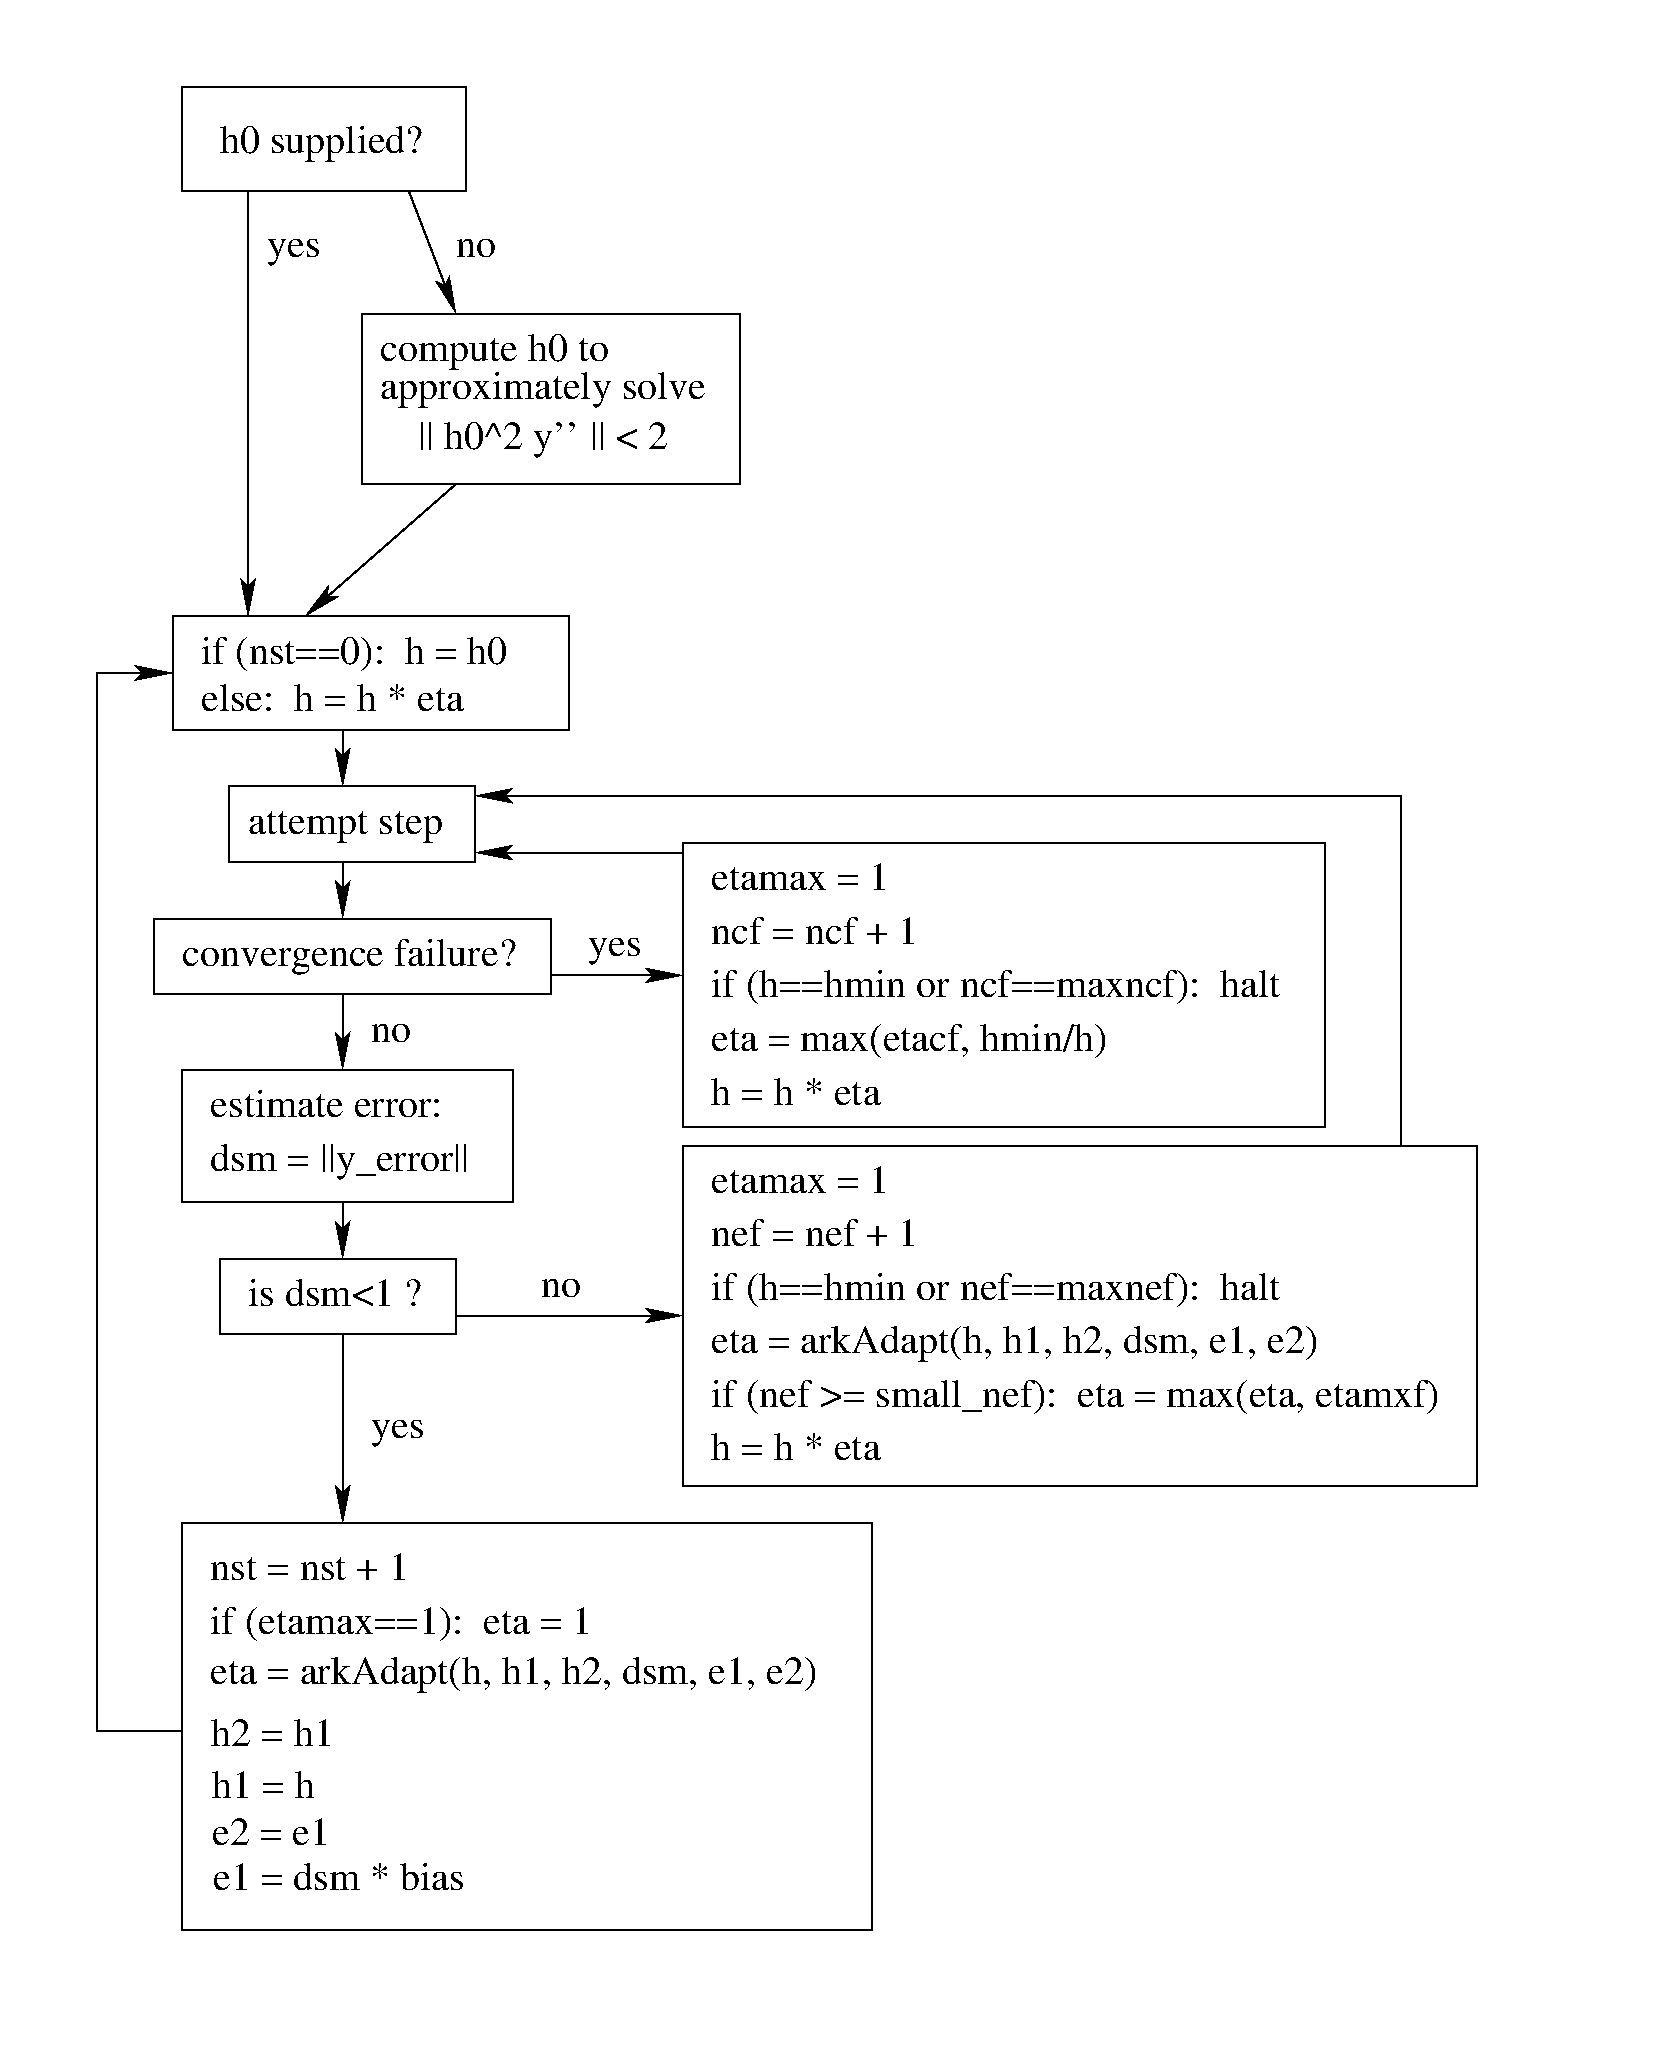
\includegraphics{time_adaptivity.png}}
\label{Mathematics:adaptivity-figure}\end{figure}

For some problems it may be preferable to avoid small step size
adjustments.  This can be especially true for problems that construct
a Newton Jacobian matrix or a preconditioner for a nonlinear or an
iterative linear solve, where this construction is computationally
expensive, and where convergence can be seriously hindered through use
of an inaccurate matrix.  To accommodate these scenarios, the step is
left unchanged when \(\eta \in [\eta_L, \eta_U]\).  The default
values for this interval are \(\eta_L = 1\) and \(\eta_U =
1.5\), and may be modified by the user.

We note that any choices for \(\eta\) (or equivalently,
\(h'\)) are subsequently constrained by the optional user-supplied
bounds \(h_\text{min}\) and \(h_\text{max}\).  Additionally,
the time-stepping algorithms in ARKode may similarly limit \(h'\)
to adhere to a user-provided ``TSTOP'' stopping point,
\(t_\text{stop}\).


\subsection{Asymptotic error control}
\label{Mathematics:asymptotic-error-control}\label{Mathematics:mathematics-adaptivity-errorcontrol}
As mentioned above, the time-stepping modules in ARKode adapt the step
size in order to attain local errors within desired tolerances of the
true solution.  These adaptivity algorithms estimate the prospective
step size \(h'\) based on the asymptotic local error estimates
\eqref{Mathematics-AsymptoticErrors}.  We define the values \(\varepsilon_n\),
\(\varepsilon_{n-1}\) and \(\varepsilon_{n-2}\) as
\begin{gather}
\begin{split}\varepsilon_k &\ \equiv \ \|T_k\|
   \ = \ \beta \|y_k - \tilde{y}_k\|,\end{split}\notag
\end{gather}
corresponding to the local error estimates for three consecutive
steps, \(t_{n-3} \to t_{n-2} \to t_{n-1} \to t_n\).  These local
error history values are all initialized to 1 upon program
initialization, to accommodate the few initial time steps of a
calculation where some of these error estimates have not yet been
computed.  With these estimates, ARKode supports a variety of error
control algorithms, as specified in the subsections below.


\subsubsection{PID controller}
\label{Mathematics:mathematics-adaptivity-errorcontrol-pid}\label{Mathematics:pid-controller}
This is the default time adaptivity controller used by the ARKStep and
ERKStep modules.  It derives from those found in \phantomsection\label{Mathematics:id7}{\hyperref[References:kc2003]{\emph{{[}KC2003{]}}}}, \phantomsection\label{Mathematics:id8}{\hyperref[References:s1998]{\emph{{[}S1998{]}}}}, \phantomsection\label{Mathematics:id9}{\hyperref[References:s2003]{\emph{{[}S2003{]}}}} and
\phantomsection\label{Mathematics:id10}{\hyperref[References:s2006]{\emph{{[}S2006{]}}}}, and uses all three of the local error estimates
\(\varepsilon_n\), \(\varepsilon_{n-1}\) and
\(\varepsilon_{n-2}\) in determination of a prospective step size,
\begin{gather}
\begin{split}h' \;=\; h_n\; \varepsilon_n^{-k_1/p}\; \varepsilon_{n-1}^{k_2/p}\;
     \varepsilon_{n-2}^{-k_3/p},\end{split}\notag
\end{gather}
where the constants \(k_1\), \(k_2\) and \(k_3\) default
to 0.58, 0.21 and 0.1, respectively, and may be modied by the user.
In this estimate, a floor of \(\varepsilon > 10^{-10}\) is
enforced to avoid division-by-zero errors.


\subsubsection{PI controller}
\label{Mathematics:pi-controller}\label{Mathematics:mathematics-adaptivity-errorcontrol-pi}
Like with the previous method, the PI controller derives from those
found in \phantomsection\label{Mathematics:id11}{\hyperref[References:kc2003]{\emph{{[}KC2003{]}}}}, \phantomsection\label{Mathematics:id12}{\hyperref[References:s1998]{\emph{{[}S1998{]}}}}, \phantomsection\label{Mathematics:id13}{\hyperref[References:s2003]{\emph{{[}S2003{]}}}} and \phantomsection\label{Mathematics:id14}{\hyperref[References:s2006]{\emph{{[}S2006{]}}}}, but it differs in
that it only uses the two most recent step sizes in its adaptivity
algorithm,
\begin{gather}
\begin{split}h' \;=\; h_n\; \varepsilon_n^{-k_1/p}\; \varepsilon_{n-1}^{k_2/p}.\end{split}\notag
\end{gather}
Here, the default values of \(k_1\) and \(k_2\) default
to 0.8 and 0.31, respectively, though they may be changed by the user.


\subsubsection{I controller}
\label{Mathematics:i-controller}\label{Mathematics:mathematics-adaptivity-errorcontrol-i}
This is the standard time adaptivity control algorithm in use by most
publicly-available ODE solver codes.  It bases the prospective time step
estimate entirely off of the current local error estimate,
\begin{gather}
\begin{split}h' \;=\; h_n\; \varepsilon_n^{-k_1/p}.\end{split}\notag
\end{gather}
By default, \(k_1=1\), but that may be modified by the user.


\subsubsection{Explicit Gustafsson controller}
\label{Mathematics:explicit-gustafsson-controller}\label{Mathematics:mathematics-adaptivity-errorcontrol-egus}
This step adaptivity algorithm was proposed in \phantomsection\label{Mathematics:id15}{\hyperref[References:g1991]{\emph{{[}G1991{]}}}}, and
is primarily useful with explicit Runge-Kutta methods.
In the notation of our earlier controllers, it has the form
\phantomsection\label{Mathematics:equation-expGus}\begin{gather}
\begin{split}h' \;=\; \begin{cases}
   h_1\; \varepsilon_1^{-1/p}, &\quad\text{on the first step}, \\
   h_n\; \varepsilon_n^{-k_1/p}\;
     \left(\varepsilon_n/\varepsilon_{n-1}\right)^{k_2/p}, &
   \quad\text{on subsequent steps}.
\end{cases}\end{split}\label{Mathematics-expGus}
\end{gather}
The default values of \(k_1\) and \(k_2\) are 0.367 and 0.268,
respectively, and may be modified by the user.


\subsubsection{Implicit Gustafsson controller}
\label{Mathematics:mathematics-adaptivity-errorcontrol-igus}\label{Mathematics:implicit-gustafsson-controller}
A version of the above controller suitable for implicit Runge-Kutta
methods was introduced in \phantomsection\label{Mathematics:id16}{\hyperref[References:g1994]{\emph{{[}G1994{]}}}}, and has the form
\phantomsection\label{Mathematics:equation-impGus}\begin{gather}
\begin{split}h' = \begin{cases}
   h_1 \varepsilon_1^{-1/p}, &\quad\text{on the first step}, \\
   h_n \left(h_n / h_{n-1}\right) \varepsilon_n^{-k_1/p}
     \left(\varepsilon_n/\varepsilon_{n-1}\right)^{-k_2/p}, &
   \quad\text{on subsequent steps}.
\end{cases}\end{split}\label{Mathematics-impGus}
\end{gather}
The algorithm parameters default to \(k_1 = 0.98\) and
\(k_2 = 0.95\), but may be modified by the user.


\subsubsection{ImEx Gustafsson controller}
\label{Mathematics:imex-gustafsson-controller}\label{Mathematics:mathematics-adaptivity-errorcontrol-iegus}
An ImEx version of these two preceding controllers is also available.
This approach computes the estimates \(h'_1\) arising from
equation \eqref{Mathematics-expGus} and the estimate \(h'_2\) arising from
equation \eqref{Mathematics-impGus}, and selects
\begin{gather}
\begin{split}h' = \frac{h}{|h|}\min\left\{|h'_1|, |h'_2|\right\}.\end{split}\notag
\end{gather}
Here, equation \eqref{Mathematics-expGus} uses \(k_1\) and
\(k_2\) with default values of 0.367 and 0.268, while equation
\eqref{Mathematics-impGus} sets both parameters to the input \(k_3\) that
defaults to 0.95.  All of these values may be modified by the user.


\subsubsection{User-supplied controller}
\label{Mathematics:mathematics-adaptivity-errorcontrol-user}\label{Mathematics:user-supplied-controller}
Finally, ARKode's time-stepping modules allow the user to define their
own time step adaptivity function,
\begin{gather}
\begin{split}h' = H(y, t, h_n, h_{n-1}, h_{n-2}, \varepsilon_n, \varepsilon_{n-1}, \varepsilon_{n-2}, q, p),\end{split}\notag
\end{gather}
to allow for problem-specific choices, or for continued
experimentation with temporal error controllers.


\section{Explicit stability}
\label{Mathematics:mathematics-stability}\label{Mathematics:explicit-stability}
For problems that involve a nonzero explicit component,
i.e. \(f^E(t,y) \ne 0\) in ARKStep or for any problem in
ERKStep, explicit and ImEx Runge-Kutta methods may benefit from
additional user-supplied information regarding the explicit stability
region.  All ARKode adaptivity methods utilize estimates of the local
error, and it is often the case that such local error control will be
sufficient for method stability, since unstable steps will typically
exceed the error control tolerances.  However, for problems in which
\(f^E(t,y)\) includes even moderately stiff components, and
especially for higher-order integration methods, it may occur that
a significant number of attempted steps will exceed the error
tolerances.  While these steps will automatically be recomputed, such
trial-and-error can result in an unreasonable number of failed steps,
increasing the cost of the computation.  In these scenarios, a
stability-based time step controller may also be useful.

Since the maximum stable explicit step for any method depends on the
problem under consideration, in that the value \((h_n\lambda)\) must
reside within a bounded stability region, where \(\lambda\) are
the eigenvalues of the linearized operator \(\partial f^E /
\partial y\), information on the maximum stable step size is not
readily available to ARKode's time-stepping modules.  However, for
many problems such information may be easily obtained through analysis
of the problem itself, e.g. in an advection-diffusion calculation
\(f^I\) may contain the stiff diffusive components and
\(f^E\) may contain the comparably nonstiff advection terms.  In
this scenario, an explicitly stable step \(h_\text{exp}\) would be
predicted as one satisfying the Courant-Friedrichs-Lewy (CFL)
stability condition for the advective portion of the problem,
\begin{gather}
\begin{split}|h_\text{exp}| < \frac{\Delta x}{|\lambda|}\end{split}\notag
\end{gather}
where \(\Delta x\) is the spatial mesh size and \(\lambda\) is
the fastest advective wave speed.

In these scenarios, a user may supply a routine to predict this
maximum explicitly stable step size, \(|h_\text{exp}|\).  If a
value for \(|h_\text{exp}|\) is supplied, it is compared against
the value resulting from the local error controller,
\(|h_\text{acc}|\), and the eventual time step used will be
limited accordingly,
\begin{gather}
\begin{split}h' = \frac{h}{|h|}\min\{c\, |h_\text{exp}|,\, |h_\text{acc}|\}.\end{split}\notag
\end{gather}
Here the explicit stability step factor \(c>0\) (often called the
``CFL number'') defaults to \(1/2\) but may be modified by the user.


\subsection{Fixed time stepping}
\label{Mathematics:mathematics-fixedstep}\label{Mathematics:fixed-time-stepping}
While both the ARKStep and ERKStep time-stepping modules are designed
for tolerance-based time step adaptivity, they additionally support a
``fixed-step'' mode.  This mode is typically used for debugging
purposes, for verification against hand-coded Runge-Kutta methods, or
for problems where the time steps should be chosen based on other
problem-specific information.  In this mode, all internal time step
adaptivity is disabled:
\begin{itemize}
\item {} 
temporal error control is disabled,

\item {} 
nonlinear or linear solver non-convergence will result in an error
(instead of a step size adjustment),

\item {} 
no check against an explicit stability condition is performed.

\end{itemize}

Additional information on this mode is provided in the sections
{\hyperref[ARKStep_c_interface/User_callable:arkstep-cinterface-optionalinputs]{\emph{\DUspan{}{ARKStep Optional Inputs}}}} and
{\hyperref[ERKStep_c_interface/User_callable:erkstep-cinterface-optionalinputs]{\emph{\DUspan{}{ERKStep Optional Inputs}}}}.


\section{Algebraic solvers}
\label{Mathematics:algebraic-solvers}\label{Mathematics:mathematics-algebraicsolvers}
When solving a problem involving either a nonzero implicit component,
\(f^I(t,y) \ne 0\), or a non-identity mass matrix,
\(M \ne I\), systems of linear or nonlinear algebraic equations
must be solved at each stage and/or step of the method.  This section
therefore focuses on the variety of mathematical methods provided in
the ARKode infrastructure for such problems, including
{\hyperref[Mathematics:mathematics-nonlinear]{\emph{\DUspan{}{nonlinear solvers}}}},
{\hyperref[Mathematics:mathematics-linear]{\emph{\DUspan{}{linear solvers}}}},
{\hyperref[Mathematics:mathematics-preconditioning]{\emph{\DUspan{}{preconditioners}}}},
{\hyperref[Mathematics:mathematics-error]{\emph{\DUspan{}{iterative solver error control}}}},
{\hyperref[Mathematics:mathematics-predictors]{\emph{\DUspan{}{implicit predictors}}}}, and techniques
used for simplifying the above solves when using non-time-dependent
{\hyperref[Mathematics:mathematics-masssolve]{\emph{\DUspan{}{mass-matrices}}}}.


\subsection{Nonlinear solver methods}
\label{Mathematics:nonlinear-solver-methods}\label{Mathematics:mathematics-nonlinear}
For both the DIRK and ARK methods corresponding to \eqref{Mathematics-IMEX_IVP} and
\eqref{Mathematics-IVP_implicit}, an implicit system
\phantomsection\label{Mathematics:equation-Residual}\begin{gather}
\begin{split}G(z_i) \equiv M z_i - h_n A^I_{i,i} f^I(t^I_{n,i}, z_i) - a_i = 0\end{split}\label{Mathematics-Residual}
\end{gather}
must be solved for each stage \(z_i, i=1,\ldots,s\), where we have
the data
\begin{gather}
\begin{split}a_i \equiv \left( y_{n-1} + h_n \sum_{j=1}^{i-1} \left[
A^E_{i,j} f^E(t^E_{n,j}, z_j) +
A^I_{i,j} f^I(t^I_{n,j}, z_j) \right] \right)\end{split}\notag
\end{gather}
for the ARK methods, or
\begin{gather}
\begin{split}a_i \equiv \left( y_{n-1} + h_n \sum_{j=1}^{i-1}
A^I_{i,j} f^I(t^I_{n,j}, z_j) \right)\end{split}\notag
\end{gather}
for the DIRK methods.  Here, if \(f^I(t,y)\) depends nonlinearly
on \(y\) then \eqref{Mathematics-Residual} corresponds to a nonlinear system of
equations; if \(f^I(t,y)\) depends linearly on \(y\) then this
is a linear system of equations.

For systems of either type, ARKode provides a choice of solution
strategies. The default solver choice is a variant of \index{Newton's
method}Newton's
method,
\phantomsection\label{Mathematics:equation-Newton_iteration}\begin{gather}
\begin{split}z_i^{(m+1)} = z_i^{(m)} + \delta^{(m+1)},\end{split}\label{Mathematics-Newton_iteration}
\end{gather}
where \(m\) is the Newton iteration index, and the \index{Newton
update}Newton
update \(\delta^{(m+1)}\) in turn requires the solution of the
\index{Newton linear system}Newton linear system
\phantomsection\label{Mathematics:equation-Newton_system}\begin{gather}
\begin{split}{\mathcal A}\left(t^I_{n,i}, z_i^{(m)}\right)\, \delta^{(m+1)} =
-G\left(z_i^{(m)}\right),\end{split}\label{Mathematics-Newton_system}
\end{gather}
in which
\phantomsection\label{Mathematics:equation-NewtonMatrix}\begin{gather}
\begin{split}{\mathcal A}(t,z) \approx M - \gamma J(t,z), \quad
J(t,z) = \frac{\partial f^I(t,z)}{\partial z}, \quad\text{and}\quad
\gamma = h_n A^I_{i,i}.\end{split}\label{Mathematics-NewtonMatrix}
\end{gather}
When the problem involves an identity mass matrix, then as an
alternative to Newton's method, ARKode provides a \index{fixed point
iteration}fixed point
iteration for solving the stages \(z_i, i=1,\ldots,s\),
\phantomsection\label{Mathematics:equation-AAFP_iteration}\begin{gather}
\begin{split}z_i^{(m+1)} = \Phi\left(z_i^{(m)}\right) \equiv z_i^{(m)} -
G\left(z_i^{(m)}\right), \quad m=0,1,\ldots\end{split}\label{Mathematics-AAFP_iteration}
\end{gather}
This iteration may additionally be improved using a technique
called ``Anderson acceleration''  \phantomsection\label{Mathematics:id17}{\hyperref[References:wn2011]{\emph{{[}WN2011{]}}}}.  Unlike with Newton's
method, these methods \emph{do not} require the solution of a linear system
at each iteration, instead opting for solution of a low-dimensional
least-squares solution to construct the nonlinear update.

Finally, if the user specifies that \(f^I(t,y)\) depends linearly
on \(y\), and if the Newton-based nonlinear solver is chosen, then
the problem \eqref{Mathematics-Residual} will be solved using only a single Newton
iteration. In this case, an additional user-supplied argument
indicates whether this Jacobian is time-dependent or not, signaling
whether the Jacobian or preconditioner needs to be recomputed
at each stage or time step, or if it can be reused throughout the full
simulation.

The optimal choice of solver (Newton vs fixed-point) is highly
problem dependent.  Since fixed-point solvers do not require the
solution of any linear systems, each iteration may be significantly
less costly than their Newton counterparts.  However, this can come at
the cost of slower convergence (or even divergence) in comparison with
Newton-like methods.  On the other hand, these fixed-point solvers do
allow for user specification of the Anderson-accelerated subspace
size, \(m_k\).  While the required amount of solver memory for
acceleration grows proportionately to \(m_k N\), larger values of
\(m_k\) may result in faster convergence.  In our experience, this
improvement is most significant for ``small'' values, e.g. \(1\le
m_k\le 5\), and that larger values of \(m_k\) may not result in
improved convergence.

While a Newton-based iteration is the default solver due
to its increased robustness on very stiff problems, we strongly
recommend that users also consider the fixed-point solver when
attempting a new problem.

For either the Newton or fixed-point solvers, it is well-known that
both the efficiency and robustness of the algorithm intimately depend
on the choice of a good initial guess.  The initial guess
for these solvers is a prediction \(z_i^{(0)}\) that is computed
explicitly from previously-computed data (e.g. \(y_{n-2}\),
\(y_{n-1}\), and \(z_j\) where \(j<i\)).  Additional
information on the specific predictor algorithms
is provided in the following section, {\hyperref[Mathematics:mathematics-predictors]{\emph{\DUspan{}{Implicit predictors}}}}.


\subsection{Linear solver methods}
\label{Mathematics:linear-solver-methods}\label{Mathematics:mathematics-linear}
When a Newton-based method is chosen for solving each nonlinear
system, a linear system of equations must be solved at each nonlinear
iteration.  For this solve ARKode provides several choices, including
the option of a user-supplied linear solver module.  The linear solver
modules distributed with SUNDIALS are organized into two families: a
\emph{direct} family comprising direct linear solvers for dense, banded or
sparse matrices, and a \emph{spils} family comprising scaled, preconditioned,
iterative (Krylov) linear solvers.  The methods offered through these
modules are as follows:
\begin{itemize}
\item {} 
dense direct solvers, using either an internal SUNDIALS
implementation or a BLAS/LAPACK implementation (serial version
only),

\item {} 
band direct solvers, using either an internal SUNDIALS
implementation or a BLAS/LAPACK implementation (serial version
only),

\item {} 
sparse direct solvers, using either the KLU sparse matrix library
\phantomsection\label{Mathematics:id18}{\hyperref[References:klu]{\emph{{[}KLU{]}}}}, or the OpenMP or PThreads-enabled SuperLU\_MT sparse matrix
library \phantomsection\label{Mathematics:id19}{\hyperref[References:superlumt]{\emph{{[}SuperLUMT{]}}}} {[}Note that users will need to download and
install the KLU or SuperLU\_MT packages independent of ARKode{]},

\item {} 
SPGMR, a scaled, preconditioned GMRES (Generalized Minimal Residual)
solver,

\item {} 
SPFGMR, a scaled, preconditioned FGMRES (Flexible Generalized Minimal
Residual) solver,

\item {} 
SPBCGS, a scaled, preconditioned Bi-CGStab (Bi-Conjugate Gradient
Stable) solver,

\item {} 
SPTFQMR, a scaled, preconditioned TFQMR (Transpose-free
Quasi-Minimal Residual) solver, or

\item {} 
PCG, a preconditioned CG (Conjugate Gradient method) solver for
symmetric linear systems.

\end{itemize}

For large stiff systems where direct methods are often infeasible, the
combination of an implicit integrator and a preconditioned
Krylov method can yield a powerful tool because it combines
established methods for stiff integration, nonlinear solver iteration,
and Krylov (linear) iteration with a problem-specific treatment of the
dominant sources of stiffness, in the form of a user-supplied
preconditioner matrix \phantomsection\label{Mathematics:id20}{\hyperref[References:bh1989]{\emph{{[}BH1989{]}}}}.  We note that the direct linear
solver modules currently provided by SUNDIALS are only designed to be
used with the serial and threaded vector representations.

\index{modified Newton iteration}

\subsubsection{Matrix-based linear solvers}
\label{Mathematics:matrix-based-linear-solvers}\label{Mathematics:index-11}\label{Mathematics:mathematics-linear-direct}
In the case that a matrix-based linear solver is used, a \emph{modified
Newton iteration} is utilized.  In a modified newton iteration, the matrix
\({\mathcal A}\) is held fixed for multiple Newton iterations.
More precisely, each Newton iteration is computed from the modified
equation
\phantomsection\label{Mathematics:equation-modified_Newton_system}\begin{gather}
\begin{split}\tilde{\mathcal A}\left(\tilde{t},\tilde{z}\right)\, \delta^{(m+1)}
= -G\left(z_i^{(m)}\right),\end{split}\label{Mathematics-modified_Newton_system}
\end{gather}
in which
\phantomsection\label{Mathematics:equation-modified_NewtonMatrix}\begin{gather}
\begin{split}\tilde{\mathcal A}(t,z) \approx M - \tilde{\gamma} J(t,z),
\quad\text{and}\quad \tilde{\gamma} = \tilde{h} A^I_{i,i}.\end{split}\label{Mathematics-modified_NewtonMatrix}
\end{gather}
Here, the solution \(\tilde{z}\), time \(\tilde{t}\), and step
size \(\tilde{h}\) upon which the modified equation rely, are
merely values of these quantities from a previous iteration.  In other
words, the matrix \(\tilde{\mathcal A}\) is only computed rarely,
and reused for repeated solves.  The frequency at which
\(\tilde{\mathcal A}\) is recomputed defaults to 20 time steps,
but may be modified by the user.

When using the dense and band SUNMatrix objects for the linear systems
\eqref{Mathematics-modified_Newton_system}, the Jacobian \(J\) may be supplied
by a user routine, or approximated internally by finite-differences.
In the case of differencing, we use the standard approximation
\begin{gather}
\begin{split}J_{i,j}(t,z) \approx \frac{f_{I,i}(t,z+\sigma_j e_j) - f_{I,i}(t,z)}{\sigma_j},\end{split}\notag
\end{gather}
where \(e_j\) is the \(j\)-th unit vector, and the increments
\(\sigma_j\) are given by
\begin{gather}
\begin{split}\sigma_j = \max\left\{ \sqrt{U}\, |z_j|, \frac{\sigma_0}{w_j} \right\}.\end{split}\notag
\end{gather}
Here \(U\) is the unit roundoff, \(\sigma_0\) is a small
dimensionless value, and \(w_j\) is the error weight defined in
\eqref{Mathematics-EWT}.  In the dense case, this approach requires \(N\)
evaluations of \(f^I\), one for each column of \(J\).  In the
band case, the columns of \(J\) are computed in groups, using the
Curtis-Powell-Reid algorithm, with the number of \(f^I\)
evaluations equal to the matrix bandwidth.

We note that with sparse and user-supplied SUNMatrix objects, the
Jacobian \emph{must} be supplied by a user routine.

\index{inexact Newton iteration}

\subsubsection{Matrix-free iterative linear solvers}
\label{Mathematics:matrix-free-iterative-linear-solvers}\label{Mathematics:mathematics-linear-iterative}\label{Mathematics:index-12}
In the case that a matrix-free iterative linear solver is chosen,
an \emph{inexact Newton iteration} is utilized.  Here, the
matrix \({\mathcal A}\) is not itself constructed since the
algorithms only require the product of this matrix with a given
vector.  Additionally, each Newton system \eqref{Mathematics-Newton_system} is not
solved completely, since these linear solvers are iterative (hence the
``inexact'' in the name). As a result. for these linear solvers
\({\mathcal A}\) is applied in a matrix-free manner,
\begin{gather}
\begin{split}{\mathcal A}(t,z)\, v = Mv - \gamma\, J(t,z)\, v.\end{split}\notag
\end{gather}
The matrix-vector products \(Mv\) \emph{must} be provided through a
user-supplied routine; the matrix-vector products \(Jv\) are
obtained by either calling an optional user-supplied routine, or
through a finite difference approximation to the directional
derivative:
\begin{gather}
\begin{split}J(t,z)\,v \approx \frac{f^I(t,z+\sigma v) - f^I(t,z)}{\sigma},\end{split}\notag
\end{gather}
where the increment \(\sigma = 1/\|v\|\) to ensure that
\(\|\sigma v\| = 1\).

As with the modified Newton method that reused \({\mathcal A}\)
between solves, the inexact Newton iteration may also recompute
the preconditioner \(P\) infrequently to balance the high costs
of matrix construction and factorization against the reduced
convergence rate that may result from a stale preconditioner.

\index{linear solver setup}

\subsubsection{Updating the linear solver}
\label{Mathematics:updating-the-linear-solver}\label{Mathematics:mathematics-linear-setup}\label{Mathematics:index-13}
In cases where recomputation of the Newton matrix
\(\tilde{\mathcal A}\) or preconditioner \(P\) is lagged,
these structures will be recomputed only in the
following circumstances:
\begin{itemize}
\item {} 
when starting the problem,

\item {} 
when more than 20 steps have been taken since the last update (this
value may be modified by the user),

\item {} 
when the value \(\tilde{\gamma}\) of \(\gamma\) at the last
update satisfies \(\left|\gamma/\tilde{\gamma} - 1\right| >
0.2\) (this value may be modified by the user),

\item {} 
when a non-fatal convergence failure just occurred,

\item {} 
when an error test failure just occurred, or

\item {} 
if the problem is linearly implicit and \(\gamma\) has
changed by a factor larger than 100 times machine epsilon.

\end{itemize}

When an update is forced due to a convergence failure, an update of
\(\tilde{\mathcal A}\) or \(P\) may or may not involve a
re-evaluation of \(J\) (in \(\tilde{\mathcal A}\)) or of
Jacobian data (in \(P\)), depending on whether errors in the
Jacobian were the likely cause of the failure.  More generally, the
decision is made to re-evaluate \(J\) (or instruct the user to
update \(P\)) when:
\begin{itemize}
\item {} 
starting the problem,

\item {} 
more than 50 steps have been taken since the last evaluation,

\item {} 
a convergence failure occurred with an outdated matrix, and the
value \(\tilde{\gamma}\) of \(\gamma\) at the last update
satisfies \(\left|\gamma/\tilde{\gamma} - 1\right| > 0.2\),

\item {} 
a convergence failure occurred that forced a step size reduction, or

\item {} 
if the problem is linearly implicit and \(\gamma\) has
changed by a factor larger than 100 times machine epsilon.

\end{itemize}

However, for linear solvers and preconditioners that do not
rely on costly matrix construction and factorization operations
(e.g. when using a geometric multigrid method as preconditioner), it
may be more efficient to update these structures more frequently than
the above heuristics specify, since the increased rate of
linear/nonlinear solver convergence may more than account for the
additional cost of Jacobian/preconditioner construction.  To this end,
a user may specify that the system matrix \({\mathcal A}\) and/or
preconditioner \(P\) should be recomputed more frequently.

As will be further discussed in the section
{\hyperref[Mathematics:mathematics-preconditioning]{\emph{\DUspan{}{Preconditioning}}}}, in the case of most Krylov methods,
preconditioning may be applied on the left, right, or on both sides of
\({\mathcal A}\), with user-supplied routines for the
preconditioner setup and solve operations.


\subsection{Iteration Error Control}
\label{Mathematics:mathematics-error}\label{Mathematics:iteration-error-control}

\subsubsection{Nonlinear iteration error control}
\label{Mathematics:nonlinear-iteration-error-control}\label{Mathematics:mathematics-error-nonlinear}
The stopping test for all of the nonlinear solver algorithms is
related to the temporal local error test, with the goal of keeping the
nonlinear iteration errors from interfering with local error control.
Denoting the final computed value of each stage solution as
\(z_i^{(m)}\), and the true stage solution solving \eqref{Mathematics-Residual}
as \(z_i\), we want to ensure that the iteration error
\(z_i - z_i^{(m)}\) is ``small'' (recall that a norm less than 1 is
already considered within an acceptable tolerance).

To this end, we first estimate the linear convergence rate \(R_i\)
of the nonlinear iteration.  We initialize \(R_i=1\), and reset it
to this value whenever \(\tilde{\mathcal A}\) or \(P\) are
updated.  After computing a nonlinear correction \(\delta^{(m)} =
z_i^{(m)} - z_i^{(m-1)}\), if \(m>0\) we update \(R_i\) as
\begin{gather}
\begin{split}R_i \leftarrow \max\{ 0.3 R_i, \left\|\delta^{(m)}\right\| / \left\|\delta^{(m-1)}\right\| \}.\end{split}\notag
\end{gather}
where the factor 0.3 is user-modifiable.

Let \(y_n^{(m)}\) denote the time-evolved solution constructed
using our approximate nonlinear stage solutions, \(z_i^{(m)}\),
and let \(y_n^{(\infty)}\) denote the time-evolved solution
constructed using \emph{exact} nonlinear stage solutions.  We then use the
estimate
\begin{gather}
\begin{split}\left\| y_n^{(\infty)} - y_n^{(m)} \right\| \approx
\max_i \left\| z_i^{(m+1)} - z_i^{(m)} \right\| \approx
\max_i R_i \left\| z_i^{(m)} - z_i^{(m-1)} \right\| =
\max_i R_i \left\| \delta^{(m)} \right\|.\end{split}\notag
\end{gather}
Therefore our convergence (stopping) test for the nonlinear iteration
for each stage is
\phantomsection\label{Mathematics:equation-NonlinearTolerance}\begin{gather}
\begin{split}R_i \left\|\delta^{(m)} \right\| < \epsilon,\end{split}\label{Mathematics-NonlinearTolerance}
\end{gather}
where the factor \(\epsilon\) has default value 0.1.  We default
to a maximum of 3 nonlinear iterations.  We also declare the
nonlinear iteration to be divergent if any of the ratios
\(\|\delta^{(m)}\| / \|\delta^{(m-1)}\| > 2.3\) with \(m>0\).
If convergence fails in the fixed point iteration, or in the Newton
iteration with \(J\) or \({\mathcal A}\) current, we reduce
the step size \(h_n\) by a factor of 0.25.  The integration will
be halted after 10 convergence failures, or if a convergence failure
occurs with \(h_n = h_\text{min}\).  However, since the
nonlinearity of \eqref{Mathematics-Residual} may vary significantly based on the
problem under consideration, these default constants may all be
modified by the user.


\subsubsection{Linear iteration error control}
\label{Mathematics:linear-iteration-error-control}\label{Mathematics:mathematics-error-linear}
When a Krylov method is used to solve the linear Newton systems
\eqref{Mathematics-Newton_system}, its errors must also be controlled.  To this end,
we approximate the linear iteration error in the solution vector
\(\delta^{(m)}\) using the preconditioned residual vector,
e.g. \(r = P{\mathcal A}\delta^{(m)} + PG\) for the case of left
preconditioning (the role of the preconditioner is further elaborated
in the next section).  In an attempt to ensure that the linear
iteration errors do not interfere with the nonlinear solution error
and local time integration error controls, we require that the norm of
the preconditioned linear residual satisfies
\phantomsection\label{Mathematics:equation-LinearTolerance}\begin{gather}
\begin{split}\|r\| \le \frac{\epsilon_L \epsilon}{10}.\end{split}\label{Mathematics-LinearTolerance}
\end{gather}
Here \(\epsilon\) is the same value as that is used above for the
nonlinear error control.  The factor of 10 is used to ensure that the
linear solver error does not adversely affect the nonlinear solver
convergence.  Smaller values for the parameter \(\epsilon_L\) are
typically useful for strongly nonlinear or very stiff ODE systems,
while easier ODE systems may benefit from a value closer to 1.  The
default value is \(\epsilon_L = 0.05\), which may be modified by
the user.  We note that for linearly
implicit problems the tolerance \eqref{Mathematics-LinearTolerance} is similarly
used for the single Newton iteration.


\subsection{Preconditioning}
\label{Mathematics:mathematics-preconditioning}\label{Mathematics:preconditioning}
When using an inexact Newton method to solve the nonlinear system
\eqref{Mathematics-Residual}, an iterative method is used repeatedly to solve
linear systems of the form \({\mathcal A}x = b\), where \(x\) is a
correction vector and \(b\) is a residual vector.  If this
iterative method is one of the scaled preconditioned iterative linear
solvers supplied with SUNDIALS, their efficiency may benefit
tremendously from preconditioning. A system \({\mathcal A}x=b\)
can be preconditioned using any one of:
\begin{gather}
\begin{split}(P^{-1}{\mathcal A})x = P^{-1}b & \qquad\text{[left preconditioning]}, \\
({\mathcal A}P^{-1})Px = b  & \qquad\text{[right preconditioning]}, \\
(P_L^{-1} {\mathcal A} P_R^{-1}) P_R x = P_L^{-1}b & \qquad\text{[left and right
preconditioning]}.\end{split}\notag
\end{gather}
These Krylov iterative methods are then applied to a system with the
matrix \(P^{-1}{\mathcal A}\), \({\mathcal A}P^{-1}\), or
\(P_L^{-1} {\mathcal A} P_R^{-1}\), instead of \({\mathcal
A}\).  In order to improve the convergence of the Krylov iteration, the
preconditioner matrix \(P\), or the product \(P_L P_R\) in the
third case, should in some sense approximate the system matrix
\({\mathcal A}\).  Simultaneously, in order to be
cost-effective the matrix \(P\) (or matrices \(P_L\) and
\(P_R\)) should be reasonably efficient to evaluate and solve.
Finding an optimal point in this trade-off between rapid
convergence and low cost can be quite challenging.  Good choices are
often problem-dependent (for example, see \phantomsection\label{Mathematics:id21}{\hyperref[References:bh1989]{\emph{{[}BH1989{]}}}} for an
extensive study of preconditioners for reaction-transport systems).

Most of the iterative linear solvers supplied with SUNDIALS allow for
all three types of preconditioning (left, right or both), although for
non-symmetric matrices \({\mathcal A}\) we know of few situations
where preconditioning on both sides is superior to preconditioning on
one side only (with the product \(P = P_L P_R\)).  Moreover, for a
given preconditioner matrix, the merits of left vs. right
preconditioning are unclear in general, so we recommend that the user
experiment with both choices.  Performance can differ between these
since the inverse of the left preconditioner is included in the linear
system residual whose norm is being tested in the Krylov algorithm.
As a rule, however, if the preconditioner is the product of two
matrices, we recommend that preconditioning be done either on the left
only or the right only, rather than using one factor on each
side.  An exception to this rule is the PCG solver, that itself
assumes a symmetric matrix \({\mathcal A}\), since the PCG
algorithm in fact applies the single preconditioner matrix \(P\)
in both left/right fashion as \(P^{-1/2} {\mathcal A} P^{-1/2}\).

Typical preconditioners are based on approximations
to the system Jacobian, \(J = \partial f^I / \partial y\).  Since
the Newton iteration matrix involved is \({\mathcal A} = M -
\gamma J\), any approximation \(\bar{J}\) to \(J\) yields a
matrix that is of potential use as a preconditioner, namely \(P =
M - \gamma \bar{J}\). Because the Krylov iteration occurs within a
Newton iteration and further also within a time integration, and since
each of these iterations has its own test for convergence, the
preconditioner may use a very crude approximation, as long as it
captures the dominant numerical features of the system.  We have
found that the combination of a preconditioner with the Newton-Krylov
iteration, using even a relatively poor approximation to the Jacobian,
can be surprisingly superior to using the same matrix without Krylov
acceleration (i.e., a modified Newton iteration), as well as to using
the Newton-Krylov method with no preconditioning.


\subsection{Implicit predictors}
\label{Mathematics:implicit-predictors}\label{Mathematics:mathematics-predictors}
For problems with implicit components, a prediction algorithm is
employed for constructing the initial guesses for each implicit
Runge-Kutta stage, \(z_i^{(0)}\).  As is well-known with nonlinear
solvers, the selection of a good initial guess can have dramatic
effects on both the speed and robustness of the solve, making the
difference between rapid quadratic convergence versus divergence of
the iteration.  To this end, a variety of prediction algorithms are
provided.  In each case, the stage guesses \(z_i^{(0)}\) are
constructed explicitly using readily-available information, including
the previous step solutions \(y_{n-1}\) and \(y_{n-2}\), as
well as any previous stage solutions \(z_j, \quad j<i\).  In most
cases, prediction is performed by constructing an interpolating
polynomial through existing data, which is then evaluated at the
desired stage time to provide an inexpensive but (hopefully)
reasonable prediction of the stage solution.  Specifically, for most
Runge-Kutta methods each stage solution satisfies
\begin{gather}
\begin{split}z_i \approx y(t^I_{n,i}),\end{split}\notag
\end{gather}
so by constructing an interpolating polynomial \(p_q(t)\) through
a set of existing data, the initial guess at stage solutions may be
approximated as
\phantomsection\label{Mathematics:equation-extrapolant}\begin{gather}
\begin{split}z_i^{(0)} = p_q(t^I_{n,i}).\end{split}\label{Mathematics-extrapolant}
\end{gather}
As the stage times for implicit ARK and DIRK stages usually satisfy
\(c_j^I > 0\), it is typically the case that \(t^I_{n,j}\) is
outside of the time interval containing the data used to construct
\(p_q(t)\), hence \eqref{Mathematics-extrapolant} will correspond to an
extrapolant instead of an interpolant.  The dangers of using a
polynomial interpolant to extrapolate values outside the interpolation
interval are well-known, with higher-order polynomials and predictions
further outside the interval resulting in the greatest potential
inaccuracies.

The prediction algorithms available in ARKode therefore
construct a variety of interpolants \(p_q(t)\), having
different polynomial order and using different interpolation data, to
support `optimal' choices for different types of problems, as
described below.


\subsubsection{Trivial predictor}
\label{Mathematics:trivial-predictor}\label{Mathematics:mathematics-predictors-trivial}
The so-called ``trivial predictor'' is given by the formula
\begin{gather}
\begin{split}p_0(t) = y_{n-1}.\end{split}\notag
\end{gather}
While this piecewise-constant interpolant is clearly not a highly
accurate candidate for problems with time-varying solutions, it is
often the most robust approach for highly stiff problems, or for
problems with implicit constraints whose violation may cause illegal
solution values (e.g. a negative density or temperature).


\subsubsection{Maximum order predictor}
\label{Mathematics:maximum-order-predictor}\label{Mathematics:mathematics-predictors-max}
At the opposite end of the spectrum, ARKode's
{\hyperref[Mathematics:mathematics-interpolation]{\emph{\DUspan{}{interpolation module}}}} can be used to
construct a higher-order polynomial interpolant, \(p_q(t)\), based on the two
most-recently-computed solutions,
\(\left\{ y_{n-2}, f_{n-2}, y_{n-1}, f_{n-1} \right\}\).
This can then be used to extrapolate predicted stage
solutions for each stage time \(t^I_{n,i}\).  This polynomial
order is the same as that specified by the user for dense output.


\subsubsection{Variable order predictor}
\label{Mathematics:variable-order-predictor}\label{Mathematics:mathematics-predictors-decreasing}
This predictor attempts to use higher-order polynomials
\(p_q(t)\) for predicting earlier stages, and lower-order
interpolants for later stages.  It uses the same interpolation module
as described above, but chooses \(q\) adaptively based on the
stage index \(i\), under the (rather tenuous) assumption that the
stage times are increasing, i.e. \(c^I_j < c^I_k\) for
\(j<k\):
\begin{gather}
\begin{split}q = \max\{ q_\text{max} - i,\; 1 \}.\end{split}\notag
\end{gather}

\subsubsection{Cutoff order predictor}
\label{Mathematics:cutoff-order-predictor}\label{Mathematics:mathematics-predictors-cutoff}
This predictor follows a similar idea as the previous algorithm, but
monitors the actual stage times to determine the polynomial
interpolant to use for prediction.  Denoting \(\tau = c_i^I
\frac{h_n}{h_{n-1}}\), the polynomial degree \(q\) is chosen as:
\begin{gather}
\begin{split}q = \begin{cases}
   q_\text{max}, & \text{if}\quad \tau < \tfrac12,\\
   1, & \text{otherwise}.
\end{cases}\end{split}\notag
\end{gather}

\subsubsection{Bootstrap predictor}
\label{Mathematics:mathematics-predictors-bootstrap}\label{Mathematics:bootstrap-predictor}
This predictor does not use any information from the preceding
step, instead using information only within the current step
\([t_{n-1},t_n]\).  In addition to using the solution and ODE
right-hand side function, \(y_{n-1}\) and
\(f(t_{n-1},y_{n-1})\), this approach uses the right-hand
side from a previously computed stage solution in the same step,
\(f(t_{n-1}+c^I_j h,z_j)\) to construct a quadratic Hermite
interpolant for the prediction.  If we define the constants
\(\tilde{h} = c^I_j h\) and \(\tau = c^I_i h\), the predictor
is given by
\begin{gather}
\begin{split}z_i^{(0)} = y_{n-1} + \left(\tau - \frac{\tau^2}{2\tilde{h}}\right)
   f(t_{n-1},y_{n-1}) + \frac{\tau^2}{2\tilde{h}} f(t_{n-1}+\tilde{h},z_j).\end{split}\notag
\end{gather}
For stages without a nonzero preceding stage time,
i.e. \(c^I_j\ne 0\) for \(j<i\), this method reduces to using
the trivial predictor \(z_i^{(0)} = y_{n-1}\).  For stages having
multiple preceding nonzero \(c^I_j\), we choose the stage having
largest \(c^I_j\) value, to minimize the level of extrapolation
used in the prediction.

We note that in general, each stage solution \(z_j\) has
significantly worse accuracy than the time step solutions
\(y_{n-1}\), due to the difference between the \emph{stage order} and
the \emph{method order} in Runge-Kutta methods.  As a result, the accuracy
of this predictor will generally be rather limited, but it is
provided for problems in which this increased stage error is better
than the effects of extrapolation far outside of the previous time
step interval \([t_{n-2},t_{n-1}]\).

We further note that although this method could be used with
non-identity mass matrix \(M\ne I\), support for that mode is not
currently implemented, so selection of this predictor in the case that
\(M\ne I\) will result in use of the trivial predictor.


\subsubsection{Minimum correction predictor}
\label{Mathematics:minimum-correction-predictor}\label{Mathematics:mathematics-predictors-minimumcorrection}
The last predictor is not interpolation based; instead it
utilizes all existing stage information from the current step to
create a predictor containing all but the current stage solution.
Specifically, as discussed in equations \eqref{Mathematics-ARK} and \eqref{Mathematics-Residual},
each stage solves a nonlinear equation
\begin{gather}
\begin{split}z_i &= y_{n-1} + h_n \sum_{j=1}^{i-1} A^E_{i,j} f^E(t^E_{n,j}, z_j)
+ h_n \sum_{j=1}^{i}   A^I_{i,j} f^I(t^I_{n,j}, z_j), \\
\Leftrightarrow \qquad \qquad & \\
G(z_i) &\equiv z_i - h_n A^I_{i,i} f^I(t^I_{n,i}, z_i) - a_i = 0.\end{split}\notag
\end{gather}
This prediction method merely computes the predictor \(z_i\) as
\begin{gather}
\begin{split}z_i &= y_{n-1} + h_n \sum_{j=1}^{i-1} A^E_{i,j} f^E(t^E_{n,j}, z_j)
              + h_n \sum_{j=1}^{i-1}  A^I_{i,j} f^I(t^I_{n,j}, z_j), \\
\Leftrightarrow \quad \qquad & \\
z_i &= a_i.\end{split}\notag
\end{gather}
We again note that although this method could be used with
non-identity mass matrix \(M\ne I\), support for that mode is not
currently implemented, so selection of this predictor in the case that
\(M\ne I\) will result in use of the trivial predictor.


\subsection{Mass matrix solver}
\label{Mathematics:mass-matrix-solver}\label{Mathematics:mathematics-masssolve}
Within the algorithms described above, there are multiple
locations where a matrix-vector product
\phantomsection\label{Mathematics:equation-mass_multiply}\begin{gather}
\begin{split}b = M v\end{split}\label{Mathematics-mass_multiply}
\end{gather}
or a linear solve
\phantomsection\label{Mathematics:equation-mass_solve}\begin{gather}
\begin{split}x = M^{-1} b\end{split}\label{Mathematics-mass_solve}
\end{gather}
are required.

Of course, for problems in which \(M=I\) both of these operators
are trivial.  However for problems with non-identity \(M\),
these linear solves \eqref{Mathematics-mass_solve} may be handled using
any valid linear solver module, in the same manner as described in the
section {\hyperref[Mathematics:mathematics-linear]{\emph{\DUspan{}{Linear solver methods}}}} for solving the linear Newton
systems.

At present, for DIRK and ARK problems using a matrix-based solver for
the Newton nonlinear iterations, the type of matrix (dense, band,
sparse, or custom) for the Jacobian matrix \(J\) must match the
type of mass matrix \(M\), since these are combined to form the
Newton system matrix \(\tilde{\mathcal A}\).  When matrix-based
methods are employed, the user must supply a routine to compute
\(M\) in the appropriate form to match the structure of
\({\mathcal A}\), with a user-supplied routine of type
{\hyperref[ARKStep_c_interface/User_supplied:c.ARKLsMassFn]{\emph{\code{ARKLsMassFn()}}}}.  This matrix structure is used internally to
perform any requisite mass matrix-vector products \eqref{Mathematics-mass_multiply}.

When matrix-free methods are selected, a routine must be supplied to
perform the mass-matrix-vector product, \(Mv\).  As with iterative
solvers for the Newton systems, preconditioning may be applied to aid
in solution of the mass matrix systems \eqref{Mathematics-mass_solve}.  When using an
iterative mass matrix linear solver, we require that the norm of the
preconditioned linear residual satisfies
\phantomsection\label{Mathematics:equation-MassLinearTolerance}\begin{gather}
\begin{split}\|r\| \le \epsilon_L \epsilon,\end{split}\label{Mathematics-MassLinearTolerance}
\end{gather}
where again, \(\epsilon\) is the nonlinear solver tolerance
parameter from \eqref{Mathematics-NonlinearTolerance}.  When using iterative system
and mass matrix linear solvers, \(\epsilon_L\) may be specified
separately for both tolerances \eqref{Mathematics-LinearTolerance} and
\eqref{Mathematics-MassLinearTolerance}.

In the above algorithmic description there are three locations
where a linear solve of the form \eqref{Mathematics-mass_solve} is required: (a) in
constructing the time-evolved solution \(y_n\), (b) in estimating
the local temporal truncation error, and (c) in constructing
predictors for the implicit solver iteration (see section
{\hyperref[Mathematics:mathematics-predictors-max]{\emph{\DUspan{}{Maximum order predictor}}}}).  Specifically, to construct the
time-evolved solution \(y_n\) from equation \eqref{Mathematics-ARK} we must
solve
\begin{gather}
\begin{split}&M y_n \ = \ M y_{n-1} + h_n \sum_{i=1}^{s} \left( b^E_i f^E(t^E_{n,i}, z_i)
              + b^I_i f^I(t^I_{n,i}, z_i)\right), \\
\Leftrightarrow \qquad & \\
&M (y_n -y_{n-1}) \ = \ h_n \sum_{i=1}^{s} \left(b^E_i f^E(t^E_{n,i}, z_i)
              + b^I_i f^I(t^I_{n,i}, z_i)\right), \\
\Leftrightarrow \qquad & \\
&M \nu \ = \ h_n \sum_{i=1}^{s} \left(b^E_i f^E(t^E_{n,i}, z_i)
              + b^I_i f^I(t^I_{n,i}, z_i)\right),\end{split}\notag
\end{gather}
for the update \(\nu = y_n - y_{n-1}\).  For construction of the
stages \(z_i\) this requires no mass matrix solves (as these are
included in the nonlinear system solve).  Similarly, in computing
the local temporal error estimate \(T_n\) from equation \eqref{Mathematics-LTE}
we must solve systems of the form
\phantomsection\label{Mathematics:equation-mass_solve_LTE}\begin{gather}
\begin{split}M\, T_n = h \sum_{i=1}^{s} \left[
\left(b^E_i - \tilde{b}^E_i\right) f^E(t^E_{n,i}, z_i) +
\left(b^I_i - \tilde{b}^I_i\right) f^I(t^I_{n,i}, z_i) \right].\end{split}\label{Mathematics-mass_solve_LTE}
\end{gather}
Lastly, in constructing dense output and implicit predictors of order
2 or higher (as in the section {\hyperref[Mathematics:mathematics-predictors-max]{\emph{\DUspan{}{Maximum order predictor}}}} above),
we must compute the derivative information \(f_k\) from the equation
\begin{gather}
\begin{split}M f_k = f^E(t_k, y_k) + f^I(t_k, y_k).\end{split}\notag
\end{gather}
In total, these require only two mass-matrix linear solves
\eqref{Mathematics-mass_solve} per attempted time step, with one more upon
completion of a time step that meets the solution accuracy
requirements.  When fixed time-stepping is used (\(h_n=h\)), the
solve \eqref{Mathematics-mass_solve_LTE} is not performed at each attempted step.


\section{Rootfinding}
\label{Mathematics:mathematics-rootfinding}\label{Mathematics:rootfinding}
Many of the time-stepping modules in ARKode also support a rootfinding
feature.  This means that, while integrating the IVP \eqref{Mathematics-IVP}, these
can also find the roots of a set of user-defined functions
\(g_i(t,y)\) that depend on \(t\) and the solution vector
\(y = y(t)\). The number of these root functions is arbitrary, and
if more than one \(g_i\) is found to have a root in any given
interval, the various root locations are found and reported in the
order that they occur on the \(t\) axis, in the direction of
integration.

Generally, this rootfinding feature finds only roots of odd
multiplicity, corresponding to changes in sign of \(g_i(t,
y(t))\), denoted \(g_i(t)\) for short. If a user root function has
a root of even multiplicity (no sign change), it will almost certainly
be missed due to the realities of floating-point arithmetic.  If such
a root is desired, the user should reformulate the root function so
that it changes sign at the desired root.

The basic scheme used is to check for sign changes of any
\(g_i(t)\) over each time step taken, and then (when a sign change
is found) to home in on the root (or roots) with a modified secant
method \phantomsection\label{Mathematics:id22}{\hyperref[References:hs1980]{\emph{{[}HS1980{]}}}}.  In addition, each time \(g\) is
evaluated, ARKode checks to see if \(g_i(t) = 0\) exactly, and if
so it reports this as a root.  However, if an exact zero of any
\(g_i\) is found at a point \(t\), ARKode computes
\(g(t+\delta)\) for a small increment \(\delta\), slightly
further in the direction of integration, and if any
\(g_i(t+\delta) = 0\) also, ARKode stops and reports an
error. This way, each time ARKode takes a time step, it is guaranteed
that the values of all \(g_i\) are nonzero at some past value of
\(t\), beyond which a search for roots is to be done.

At any given time in the course of the time-stepping, after suitable
checking and adjusting has been done, ARKode has an interval
\((t_\text{lo}, t_\text{hi}]\) in which roots of the
\(g_i(t)\) are to be sought, such that \(t_\text{hi}\) is
further ahead in the direction of integration, and all
\(g_i(t_\text{lo}) \ne 0\).  The endpoint \(t_\text{hi}\) is
either \(t_n\), the end of the time step last taken, or the next
requested output time \(t_\text{out}\) if this comes sooner. The
endpoint \(t_\text{lo}\) is either \(t_{n-1}\), or the last
output time \(t_\text{out}\) (if this occurred within the last
step), or the last root location (if a root was just located within
this step), possibly adjusted slightly toward \(t_n\) if an exact
zero was found. The algorithm checks \(g(t_\text{hi})\) for zeros, and
it checks for sign changes in \((t_\text{lo}, t_\text{hi})\). If no sign
changes are found, then either a root is reported (if some
\(g_i(t_\text{hi}) = 0\)) or we proceed to the next time interval
(starting at \(t_\text{hi}\)). If one or more sign changes were found,
then a loop is entered to locate the root to within a rather tight
tolerance, given by
\begin{gather}
\begin{split}\tau = 100\, U\, (|t_n| + |h|)\qquad (\text{where}\; U = \text{unit roundoff}).\end{split}\notag
\end{gather}
Whenever sign changes are seen in two or more root functions, the one
deemed most likely to have its root occur first is the one with the
largest value of
\(\left|g_i(t_\text{hi})\right| / \left| g_i(t_\text{hi}) - g_i(t_\text{lo})\right|\),
corresponding to the closest to \(t_\text{lo}\) of the secant method
values. At each pass through the loop, a new value \(t_\text{mid}\) is
set, strictly within the search interval, and the values of
\(g_i(t_\text{mid})\) are checked. Then either \(t_\text{lo}\) or
\(t_\text{hi}\) is reset to \(t_\text{mid}\) according to which
subinterval is found to have the sign change. If there is none in
\((t_\text{lo}, t_\text{mid})\) but some \(g_i(t_\text{mid}) = 0\), then that
root is reported. The loop continues until \(\left|t_\text{hi} -
t_\text{lo} \right| < \tau\), and then the reported root location is
\(t_\text{hi}\).  In the loop to locate the root of \(g_i(t)\), the
formula for \(t_\text{mid}\) is
\begin{gather}
\begin{split}t_\text{mid} = t_\text{hi} -
\frac{g_i(t_\text{hi}) (t_\text{hi} - t_\text{lo})}{g_i(t_\text{hi}) - \alpha g_i(t_\text{lo})} ,\end{split}\notag
\end{gather}
where \(\alpha\) is a weight parameter. On the first two passes
through the loop, \(\alpha\) is set to 1, making \(t_\text{mid}\)
the secant method value. Thereafter, \(\alpha\) is reset according
to the side of the subinterval (low vs high, i.e. toward
\(t_\text{lo}\) vs toward \(t_\text{hi}\)) in which the sign change was
found in the previous two passes. If the two sides were opposite,
\(\alpha\) is set to 1. If the two sides were the same, \(\alpha\)
is halved (if on the low side) or doubled (if on the high side). The
value of \(t_\text{mid}\) is closer to \(t_\text{lo}\) when
\(\alpha < 1\) and closer to \(t_\text{hi}\) when \(\alpha > 1\).
If the above value of \(t_\text{mid}\) is within \(\tau /2\) of
\(t_\text{lo}\) or \(t_\text{hi}\), it is adjusted inward, such that its
fractional distance from the endpoint (relative to the interval size)
is between 0.1 and 0.5 (with 0.5 being the midpoint), and the actual
distance from the endpoint is at least \(\tau/2\).

Finally, we note that when running in parallel, ARKode's rootfinding
module assumes that the entire set of root defining functions
\(g_i(t,y)\) is replicated on every MPI task.  Since in these
cases the vector \(y\) is distributed across tasks, it is the
user's responsibility to perform any necessary inter-task
communication to ensure that \(g_i(t,y)\) is identical on each task.


\section{Inequality Constraints}
\label{Mathematics:inequality-constraints}\label{Mathematics:mathematics-inequalityconstraints}
ARKode permits the user to impose optional inequality constraints on individual
components of the solution vector \(y\). Any of the following four
constraints can be imposed: \(y_i > 0\), \(y_i < 0\),
\(y_i \geq 0\), or \(y_i \leq 0\). The constraint satisfaction is tested
after a successful step and before the error test. If any constraint fails, the
step size is reduced and a flag is set to update the Jacobian or preconditioner
if applicable. Rather than cutting the step size by some arbitrary factor,
ARKode estimates a new step size \(h'\) using a linear approximation of the
components in \(y\) that failed the constraint test (including a safety
factor of 0.9 to cover the strict inequality case). If a step fails to satisfy
the constraints 10 times (a value which may be modified by the user) within a
step attempt or fails with the minimum step size then the integration is halted
and an error is returned. In this case the user may need to employ other
strategies as discussed in {\hyperref[ARKStep_c_interface/User_callable:arkstep-cinterface-tolerances]{\emph{\DUspan{}{ARKStep tolerance specification functions}}}} and
{\hyperref[ERKStep_c_interface/User_callable:erkstep-cinterface-tolerances]{\emph{\DUspan{}{ERKStep tolerance specification functions}}}} to satisfy the inequality constraints.


\chapter{Code Organization}
\label{Organization:organization}\label{Organization::doc}\label{Organization:code-organization}
The family of solvers referred to as SUNDIALS consists of the solvers
CVODE and ARKode (for ODE systems), KINSOL (for nonlinear algebraic
systems), and IDA (for differential-algebraic systems).  In addition,
SUNDIALS also includes variants of CVODE and IDA with sensitivity analysis
capabilities (using either forward or adjoint methods), called CVODES and
IDAS, respectively.

The various solvers of this family share many subordinate modules.
For this reason, it is organized as a family, with a directory
structure that exploits that sharing (see the following Figures
{\hyperref[Organization:sunorg1]{\emph{\DUspan{}{SUNDIALS organization}}}},
{\hyperref[Organization:sunorg2]{\emph{\DUspan{}{SUNDIALS tree}}}} and
{\hyperref[Organization:sunorg3]{\emph{\DUspan{}{SUNDIALS examples}}}}).  The following is a list of the
solver packages presently available, and the basic functionality
of each:
\begin{itemize}
\item {} 
CVODE, a linear multistep solver for stiff and nonstiff ODE systems
\(\dot{y} = f(t,y)\) based on Adams and BDF methods;

\item {} 
CVODES, a linear multistep solver for stiff and nonstiff ODEs with
sensitivity analysis capabilities;

\item {} 
ARKode, a Runge-Kutta based solver for stiff, nonstiff, and mixed ODE systems;

\item {} 
IDA, a linear multistep solver for differential-algebraic systems
\(F(t,y,\dot{y}) = 0\) based on BDF methods;

\item {} 
IDAS, a linear multistep solver for differential-algebraic systems with sensitivity
analysis capabilities;

\item {} 
KINSOL, a solver for nonlinear algebraic systems \(F(u) = 0\).

\end{itemize}
\begin{figure}[htbp]
\centering
\capstart

\scalebox{0.750000}{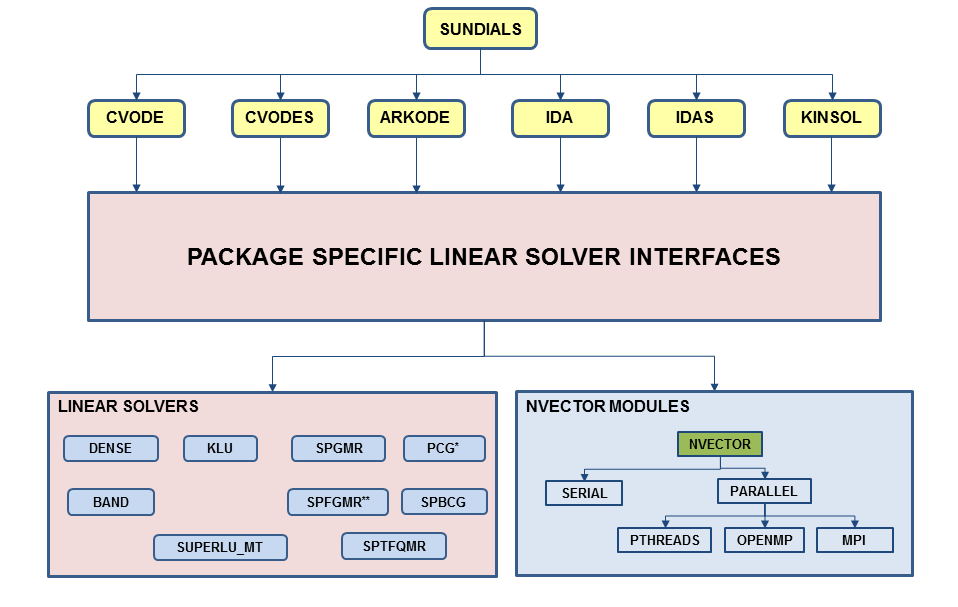
\includegraphics{sunorg1.png}}
\caption{\emph{SUNDIALS organization}: High-level diagram of the SUNDIALS structure}\label{Organization:sunorg1}\end{figure}
\begin{figure}[htbp]
\centering
\capstart

\scalebox{0.750000}{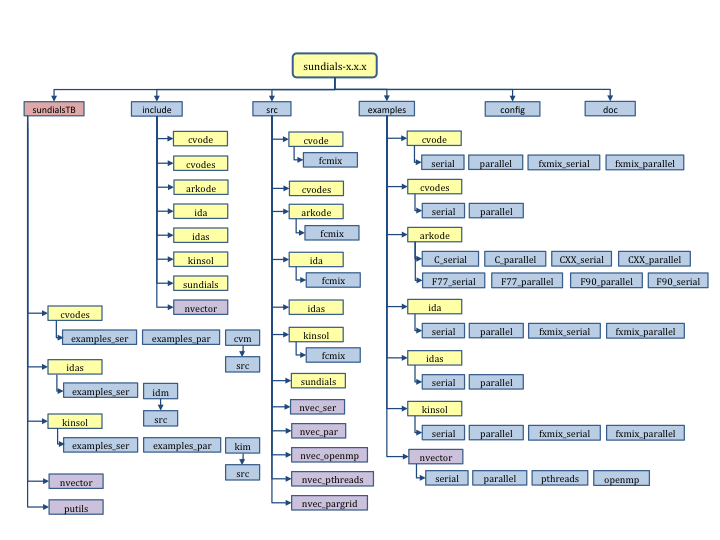
\includegraphics{sunorg2.png}}
\caption{\emph{SUNDIALS tree}: Directory structure of the source tree.}\label{Organization:sunorg2}\end{figure}
\begin{figure}[htbp]
\centering
\capstart

\scalebox{0.750000}{\includegraphics{sunorg3.png}}
\caption{\emph{SUNDIALS examples}: Directory structure of the examples.}\label{Organization:sunorg3}\end{figure}


\section{ARKode organization}
\label{Organization:arkode-organization}
The ARKode package is written in the ANSI C language.  The
following summarizes the basic structure of the package, although
knowledge of this structure is not necessary for its use.

The overall organization of the ARKode package is shown in Figure
{\hyperref[Organization:arkorg]{\emph{\DUspan{}{ARKode organization}}}}.  The central integration modules,
implemented in the files \code{arkode.h}, \code{arkode\_impl.h},
\code{arkode\_butcher.h}, \code{arkode.c}, \code{arkode\_arkstep.c} ,
\code{arkode\_erkstep.c} and \code{arkode\_butcher.c}, deal with the
evaluation of integration stages, the nonlinear solvers, estimation of
the local truncation error, selection of step size, and interpolation
to user output points, among other issues.  ARKode currently supports
modified Newton, inexact Newton, and accelerated fixed-point solvers
for these nonlinearly implicit problems.  However, when using the
Newton-based iterations, or when using a non-identity mass matrix
\(M\ne I\), ARKode has flexibility in the choice of method used to
solve the linear sub-systems that arise.  Therefore, for any user
problem invoking the Newton solvers, or any user problem with
\(M\ne I\), one (or more) of the linear system solver modules
should be specified by the user, which is then invoked as needed
during the integration process.
\begin{figure}[htbp]
\centering
\capstart

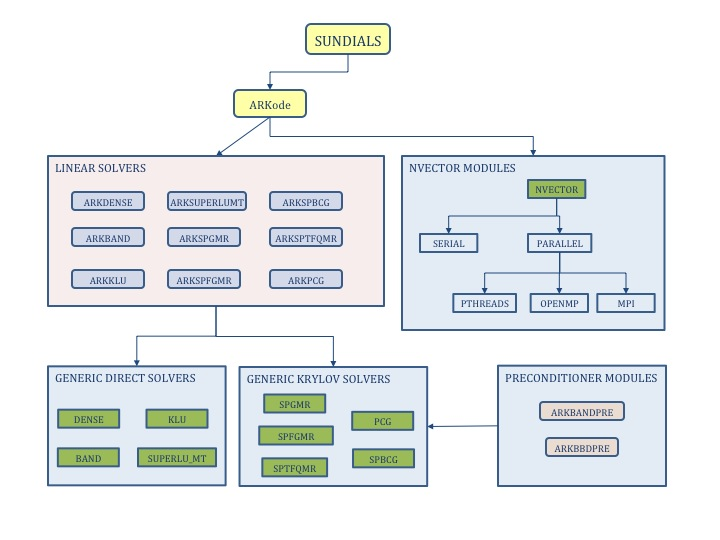
\includegraphics{arkorg.png}
\caption{\emph{ARKode organization}: Overall structure of the ARKode package.
Modules specific to ARKode are the timesteppers, linear solver
interfaces and preconditioners: ARKSTEP, ERKSTEP, ARKBBDPRE,
ARKBANDPRE; all other items correspond to generic solver
and auxiliary modules.  Note also that the LAPACK, KLU and
SuperLU\_MT support is through interfaces to external packages.
Users will need to download and compile those packages independently.}\label{Organization:arkorg}\end{figure}

For solving these linear systems, ARKode's linear solver interface
supports both direct and iterative linear solvers built using the
generic SUNLINSOL API (see {\hyperref[sunlinsol/index:sunlinsol]{\emph{\DUspan{}{Description of the SUNLinearSolver module}}}}).  These solvers may
utilize a SUNMATRIX object for storing Jacobian information, or they
may be matrix-free.  Since ARKode can operate on any valid SUNLINSOL
implementation, the set of linear solver modules available to ARKode
will expand as new SUNLINSOL modules are developed.

For users employing dense or banded Jacobians, ARKode includes
algorithms for their approximation  through difference quotients,
although the user also has the option of supplying a routine to
compute the Jacobian (or an approximation to it) directly.  This
user-supplied routine is required when using sparse or user-supplied
Jacobian matrices.

For users employing iterative linear solvers, ARKode includes an
algorithm for the approximation by difference quotients of the product
\(Av\). Again, the user has the option of providing routines for
this operation, in two phases: setup (preprocessing of Jacobian data)
and multiplication.

When solve problems with non-identity mass matrices, corresponding
user-supplied routines for computing either the mass matrix \(M\)
or the product \(Mv\) are required.  Additionally, the type of
linear solver module (iterative, dense-direct, band-direct,
sparse-direct) used for both the IVP system and mass matrix must
match.

For preconditioned iterative methods for either the system or mass
matrix solves, the preconditioning must be supplied by the user, again
in two phases: setup and solve.  While there is no default choice of
preconditioner analogous to the difference-quotient approximation in
the direct case, the references \phantomsection\label{Organization:id1}{\hyperref[References:bh1989]{\emph{{[}BH1989{]}}}} and \phantomsection\label{Organization:id2}{\hyperref[References:b1992]{\emph{{[}B1992{]}}}}, together with
the example and demonstration programs included with ARKode and CVODE,
offer considerable assistance in building simple preconditioners.

ARKode's linear solver interface consists of four primary phases,
devoted to
\begin{enumerate}
\item {} 
memory allocation and initialization,

\item {} 
setup of the matrix/preconditioner data involved,

\item {} 
solution of the system, and

\item {} 
freeing of memory.

\end{enumerate}

The setup and solution phases are separate because the evaluation of
Jacobians and preconditioners is done only periodically during the
integration process, and only as required to achieve convergence.

ARKode also provides two rudimentary preconditioner modules, for
use with any of the Krylov iterative linear solvers.  The first,
ARKBANDPRE is intended to be used with the serial or threaded vector
data structures (NVECTOR\_SERIAL, NVECTOR\_OPENMP and NVECTOR\_PTHREADS),
and provides a banded difference-quotient approximation to the
Jacobian as the preconditioner, with corresponding setup and solve
routines.  The second preconditioner module, ARKBBDPRE, is intended to
work with the parallel vector data structure, NVECTOR\_PARALLEL, and
generates a preconditioner that is a block-diagonal matrix with each
block being a band matrix owned by a single processor.

All state information used by ARKode to solve a given problem is
saved in a single opaque memory structure, and a pointer to that
structure is returned to the user.  For C and C++ applications there
is no global data in the ARKode package, and so in this respect it is
reentrant.  State information specific to the linear solver interface
is saved in a separate data structure, a pointer to which resides in
the ARKode memory structure.  State information specific to the linear
solver implementation (and matrix implementation, if applicable) are
stored in their own data structures, that are returned to the user
upon construction, and subsequently provided to ARKode for use.  We
note that the ARKode Fortran interface, however, currently uses global
variables, so at most one of each of these objects may be created per
memory space (i.e. one per MPI task in distributed memory
computations).


\chapter{Using ARKStep for C and C++ Applications}
\label{ARKStep_c_interface/index:arkstep-cinterface}\label{ARKStep_c_interface/index::doc}\label{ARKStep_c_interface/index:using-arkstep-for-c-and-c-applications}
This chapter is concerned with the use of the ARKStep time-stepping
module for the solution of initial value problems (IVPs) in a C or C++
language setting.  The following sections discuss the header files and
the layout of the user's main program, and provide descriptions of the
ARKStep user-callable functions and user-supplied functions.

The example programs described in the companion document \phantomsection\label{ARKStep_c_interface/index:id1}{\hyperref[References:r2018]{\emph{{[}R2018{]}}}} may
be helpful. Those codes may be used as templates for new codes and are
included in the ARKode package \code{examples} subdirectory.

Users with applications written in Fortran should see the chapter
{\hyperref[ARKode_f_interface/FARKODE:fortraninterface]{\emph{\DUspan{}{FARKODE, an Interface Module for FORTRAN Applications}}}}, which describes the Fortran/C interface
module for ARKStep, and may look to the Fortran example programs also
described in the companion document \phantomsection\label{ARKStep_c_interface/index:id2}{\hyperref[References:r2018]{\emph{{[}R2018{]}}}}.  These codes are also
located in the ARKode package \code{examples} directory.

The user should be aware that not all SUNLINSOL, SUNMATRIX, and
preconditioning modules are compatible with all NVECTOR
implementations.  Details on compatibility are given in the
documentation for each SUNMATRIX (see {\hyperref[sunmatrix/index:sunmatrix]{\emph{\DUspan{}{Matrix Data Structures}}}}) and each
SUNLINSOL module (see {\hyperref[sunlinsol/index:sunlinsol]{\emph{\DUspan{}{Description of the SUNLinearSolver module}}}}). For example, NVECTOR\_PARALLEL
is not compatible with the dense, banded, or sparse SUNMATRIX types,
or with the corresponding dense, banded, or sparse SUNLINSOL modules.
Please check the sections {\hyperref[sunmatrix/index:sunmatrix]{\emph{\DUspan{}{Matrix Data Structures}}}} and {\hyperref[sunlinsol/index:sunlinsol]{\emph{\DUspan{}{Description of the SUNLinearSolver module}}}} to
verify compatibility between these modules.  In addition to that
documentation, we note that the ARKBANDPRE preconditioning module is
only compatible with the NVECTOR\_SERIAL, NVECTOR\_OPENMP or
NVECTOR\_PTHREADS vector implementations, and the preconditioner module
ARKBBDPRE can only be used with NVECTOR\_PARALLEL.

ARKStep uses various input and output constants from the shared ARKode
infrastructure. These are defined as needed in this chapter, but for
convenience the full list is provided separately in the section
{\hyperref[Constants:constants]{\emph{\DUspan{}{Appendix: ARKode Constants}}}}.

The relevant information on using ARKStep's C and C++ interfaces is
detailed in the following sub-sections.


\section{Access to library and header files}
\label{ARKStep_c_interface/General:arkstep-cinterface-headers}\label{ARKStep_c_interface/General:access-to-library-and-header-files}\label{ARKStep_c_interface/General::doc}
At this point, it is assumed that the installation of ARKode,
following the procedure described in the section {\hyperref[Install:installation]{\emph{\DUspan{}{ARKode Installation Procedure}}}},
has been completed successfully.

Regardless of where the user's application program resides, its
associated compilation and load commands must make reference to the
appropriate locations for the library and header files required by
ARKode. The relevant library files are
\begin{itemize}
\item {} 
\code{libdir/libsundials\_arkode.lib},

\item {} 
\code{libdir/libsundials\_nvec*.lib},

\end{itemize}

where the file extension \code{.lib} is typically \code{.so} for shared
libraries and \code{.a} for static libraries.  The relevant header files
are located in the subdirectories
\begin{itemize}
\item {} 
\code{incdir/include/arkode}

\item {} 
\code{incdir/include/sundials}

\item {} 
\code{incdir/include/nvector}

\item {} 
\code{incdir/include/sunmatrix}

\item {} 
\code{incdir/include/sunlinsol}

\item {} 
\code{incdir/include/sunnonlinsol}

\end{itemize}

The directories \code{libdir} and \code{incdir} are the installation library
and include directories, respectively.  For a default installation,
these are \code{instdir/lib} and \code{instdir/include}, respectively, where
\code{instdir} is the directory where SUNDIALS was installed (see the
section {\hyperref[Install:installation]{\emph{\DUspan{}{ARKode Installation Procedure}}}} for further details).


\section{Data Types}
\label{ARKStep_c_interface/General:arkstep-cinterface-datatypes}\label{ARKStep_c_interface/General:data-types}
The \code{sundials\_types.h} file contains the definition of the variable
type \code{realtype}, which is used by the SUNDIALS solvers for all
floating-point data, the definition of the integer type
\code{sunindextype}, which is used for vector and matrix indices, and
\code{booleantype}, which is used for certain logic operations within
SUNDIALS.


\subsection{Floating point types}
\label{ARKStep_c_interface/General:floating-point-types}
The type ``\index{realtype}realtype'' can be set to
\code{float}, \code{double}, or \code{long double}, depending on how SUNDIALS
was installed (with the default being \code{double}). The user can change
the precision of the SUNDIALS solvers' floating-point arithmetic at the
configuration stage (see the section {\hyperref[Install:installation-cmake-options]{\emph{\DUspan{}{Configuration options (Unix/Linux)}}}}).

Additionally, based on the current precision, \code{sundials\_types.h}
defines the values \index{BIG\_REAL}BIG\_REAL to be the largest value
representable as a \code{realtype}, \index{SMALL\_REAL}SMALL\_REAL to be the
smallest positive value representable as a \code{realtype}, and
\index{UNIT\_ROUNDOFF}UNIT\_ROUNDOFF to be the smallest realtype number,
\(\varepsilon\), such that \(1.0 + \varepsilon \ne 1.0\).

Within SUNDIALS, real constants may be set to have the appropriate
precision by way of a macro called \index{RCONST}RCONST.  It is this macro
that needs the ability to branch on the definition \code{realtype}.  In
ANSI C, a floating-point constant with no suffix is stored as a
\code{double}. Placing the suffix ``F'' at the end of a floating point
constant makes it a \code{float}, whereas using the suffix ``L'' makes it a
\code{long double}. For example,

\begin{Verbatim}[commandchars=\\\{\}]
\PYG{c+cp}{\PYGZsh{}}\PYG{c+cp}{define A 1.0}
\PYG{c+cp}{\PYGZsh{}}\PYG{c+cp}{define B 1.0F}
\PYG{c+cp}{\PYGZsh{}}\PYG{c+cp}{define C 1.0L}
\end{Verbatim}

defines \code{A} to be a \code{double} constant equal to 1.0, \code{B} to be a
\code{float} constant equal to 1.0, and \code{C} to be a \code{long double} constant
equal to 1.0.  The macro call \code{RCONST(1.0)} automatically expands to
1.0 if \code{realtype} is \code{double}, to \code{1.0F} if \code{realtype} is \code{float}, or
to \code{1.0L} if \code{realtype} is \code{long double}. SUNDIALS uses the \code{RCONST}
macro internally to declare all of its floating-point constants.

Additionally, SUNDIALS defines several macros for common mathematical
functions \emph{e.g.}\}, \code{fabs}, \code{sqrt}, \code{exp}, etc. in \code{sundials\_math.h}. The
macros are prefixed with \code{SUNR} and expand to the appropriate C function based
on the \code{realtype}. For example, the macro \code{SUNRabs} expands to the C
function \code{fabs} when \code{realtype} is \code{double}, \code{fabsf} when \code{realtype}
is \code{float}, and \code{fabsl} when \code{realtype} is \code{long double}.

A user program which uses the type \code{realtype}, the \code{RCONST} macro, and the
\code{SUNR} mathematical function macros is precision-independent except for any
calls to precision-specific library functions. Our example programs use
\code{realtype}, \code{RCONST}, and the \code{SUNR} macros. Users can, however, use the
type \code{double}, \code{float}, or \code{long double} in their code (assuming that this
usage is consistent with the typedef for \code{realtype}) and call the appropriate
math library functions directly. Thus, a previously existing piece of ANSI C
code can use SUNDIALS without modifying the code to use \code{realtype},
\code{RCONST}, or the \code{SUNR} macros so long as the SUNDIALS libraries use
the correct precision (for details see {\hyperref[Install:installation]{\emph{\DUspan{}{ARKode Installation Procedure}}}}).


\subsection{Integer types used for indexing}
\label{ARKStep_c_interface/General:integer-types-used-for-indexing}
The type \code{sunindextype} is used for indexing array entries in SUNDIALS modules
(\emph{e.g.}, vectors lengths and matrix sizes) as well as for storing the total
problem size. During configuration \code{sunindextype} may be selected to be either
a 32- or 64-bit \emph{signed} integer with the default being 64-bit. See the section
{\hyperref[Install:installation]{\emph{\DUspan{}{ARKode Installation Procedure}}}} for the configuration option to select the desired size of
\code{sunindextype}. When using a 32-bit integer the total problem size is limited
to \(2^{31}-1\) and with 64-bit integers the limit is \(2^{63}-1\). For
users with problem sizes that exceed the 64-bit limit an advanced configuration
option is available to specify the type used for \code{sunindextype}.

A user program which uses \code{sunindextype} to handle indices will work with both
index storage types except for any calls to index storage-specific external
libraries. Our C and C++ example programs use \code{sunindextype}. Users can,
however, use any compatible type (\emph{e.g.},  \code{int}, \code{long int}, \code{int32\_t},
\code{int64\_t} or \code{long long int}) in their code, assuming that this usage is
consistent with the typedef for \code{sunindextype} on their architecture. Thus, a
previously existing piece of ANSI C code can use SUNDIALS without modifying the
code to use \code{sunindextype}, so long as the SUNDIALS libraries use the
appropriate index storage type (for details {\hyperref[Install:installation]{\emph{\DUspan{}{ARKode Installation Procedure}}}}).


\section{Header Files}
\label{ARKStep_c_interface/General:header-files}
When using ARKStep, the calling program must include several header
files so that various macros and data types can be used. The header
file that is always required is:
\begin{itemize}
\item {} 
\code{arkode/arkode\_arkstep.h}, the main header file for the ARKStep
time-stepping module, which defines the several types and various
constants, includes function prototypes, and includes the shared
\code{arkode/arkode.h} and \code{arkode/arkode\_ls.h} header files.

\end{itemize}

Note that \code{arkode.h} includes \code{sundials\_types.h} directly, which
defines the types \code{realtype},  \code{sunindextype} and \code{booleantype}
and the constants \code{SUNFALSE} and \code{SUNTRUE}, so a user program does
not need to include \code{sundials\_types.h} directly.

Additionally, the calling program must also include a NVECTOR
implementation header file, of the form \code{nvector/nvector\_***.h},
corresponding to the user's preferred data layout and form of
parallelism.  See the section {\hyperref[nvectors/index:nvectors]{\emph{\DUspan{}{Vector Data Structures}}}} for details for the
appropriate name.  This file in turn includes the header file
\code{sundials\_nvector.h} which defines the abstract \code{N\_Vector} data
type.

If the user includes a non-trivial implicit component to their
ODE system, then each time step will require a nonlinear solver for
the resulting systems of equations -- the default for this is a
modified Newton iteration.  If using a non-default nonlinear solver
module, or when interacting with a SUNNONLINSOL module directly, the
calling program must also include a SUNNONLINSOL header file, of the
form \code{sunnonlinsol/sunnonlinsol\_***.h} where \code{***} is the name of
the nonlinear solver module (see the section {\hyperref[sunnonlinsol/index:sunnonlinsol]{\emph{\DUspan{}{Description of the SUNNonlinearSolver Module}}}} for
more information).  This file in turn includes the header file
\code{sundials\_nonlinearsolver.h} which defines the abstract
\code{SUNNonlinearSolver} data type.

If using a nonlinear solver that requires the solution of a linear
system of the form \(\mathcal{A}x=b\) (e.g., the default Newton
iteration), then a linear solver module header file will also
be required.  Similarly, if the ODE system involves a non-identity
mass matrix \(M \ne I\), then each time step will require a linear
solver for systems of the form \(Mx=b\).  The header files
corresponding to the SUNDIALS-provided linear solver modules available
for use with ARKode are:
\begin{itemize}
\item {} 
Direct linear solvers:
\begin{itemize}
\item {} 
\code{sunlinsol/sunlinsol\_dense.h},
which is used with the dense linear solver module,
SUNLINSOL\_DENSE;

\item {} 
\code{sunlinsol/sunlinsol\_band.h},
which is used with the banded linear solver module,
SUNLINSOL\_BAND;

\item {} 
\code{sunlinsol/sunlinsol\_lapackdense.h},
which is used with the LAPACK dense linear solver module,
SUNLINSOL\_LAPACKDENSE;

\item {} 
\code{sunlinsol/sunlinsol\_lapackband.h},
which is used with the LAPACK banded linear solver module,
SUNLINSOL\_LAPACKBAND;

\item {} 
\code{sunlinsol/sunlinsol\_klu.h},
which is used with the KLU sparse linear solver module,
SUNLINSOL\_KLU;

\item {} 
\code{sunlinsol/sunlinsol\_superlumt.h},
which is used with the SuperLU\_MT sparse linear solver module,
SUNLINSOL\_SUPERLUMT;

\end{itemize}

\item {} 
Iterative linear solvers:
\begin{itemize}
\item {} 
\code{sunlinsol/sunlinsol\_spgmr.h},
which is used with the scaled, preconditioned GMRES Krylov linear
solver module, SUNLINSOL\_SPGMR;

\item {} 
\code{sunlinsol/sunlinsol\_spfgmr.h},
which is used with the scaled, preconditioned FGMRES Krylov linear
solver module, SUNLINSOL\_SPFGMR;

\item {} 
\code{sunlinsol/sunlinsol\_spbcgs.h},
which is used with the scaled, preconditioned Bi-CGStab Krylov
linear solver module, SUNLINSOL\_SPBCGS;

\item {} 
\code{sunlinsol/sunlinsol\_sptfqmr.h},
which is used with the scaled, preconditioned TFQMR Krylov linear
solver module, SUNLINSOL\_SPTFQMR;

\item {} 
\code{sunlinsol/sunlinsol\_pcg.h},
which is used with the scaled, preconditioned CG Krylov linear
solver module, SUNLINSOL\_PCG;

\end{itemize}

\end{itemize}

The header files for the SUNLINSOL\_DENSE and SUNLINSOL\_LAPACKDENSE
linear solver modules include the file
\code{sunmatrix/sunmatrix\_dense.h}, which defines the SUNMATRIX\_DENSE
matrix module, as well as various functions and macros for acting on
such matrices.

The header files for the SUNLINSOL\_BAND and SUNLINSOL\_LAPACKBAND
linear solver modules include the file \code{sunmatrix/sunmatrix\_band.h},
which defines the SUNMATRIX\_BAND matrix module, as well as various
functions and macros for acting on such matrices.

The header files for the SUNLINSOL\_KLU and SUNLINSOL\_SUPERLUMT linear
solver modules include the file \code{sunmatrix/sunmatrix\_sparse.h},
which defines the SUNMATRIX\_SPARSE matrix module, as well as various
functions and macros for acting on such matrices.

The header files for the Krylov iterative solvers include the file
\code{sundials/sundials\_iterative.h}, which enumerates the
preconditioning type and (for the SPGMR and SPFGMR solvers) the
choices for the Gram-Schmidt orthogonalization process.

Other headers may be needed, according to the choice of
preconditioner, etc.  For example, if preconditioning for an iterative
linear solver were performed using the ARKBBDPRE module, the header
\code{arkode/arkode\_bbdpre.h} is needed to access the preconditioner
initialization routines.


\section{A skeleton of the user's main program}
\label{ARKStep_c_interface/Skeleton:arkstep-cinterface-skeleton}\label{ARKStep_c_interface/Skeleton::doc}\label{ARKStep_c_interface/Skeleton:a-skeleton-of-the-user-s-main-program}
The following is a skeleton of the user's main program (or calling
program) for the integration of an ODE IVP using the ARKStep module.
Most of the steps are independent of the NVECTOR, SUNMATRIX, SUNLINSOL
and SUNNONLINSOL implementations used.  For the steps that are not,
refer to the sections {\hyperref[nvectors/index:nvectors]{\emph{\DUspan{}{Vector Data Structures}}}}, {\hyperref[sunmatrix/index:sunmatrix]{\emph{\DUspan{}{Matrix Data Structures}}}},
{\hyperref[sunlinsol/index:sunlinsol]{\emph{\DUspan{}{Description of the SUNLinearSolver module}}}}, and  {\hyperref[sunnonlinsol/index:sunnonlinsol]{\emph{\DUspan{}{Description of the SUNNonlinearSolver Module}}}} for the specific name of
the function to be called or macro to be referenced.

\index{User main program}\begin{enumerate}
\item {} 
Initialize parallel or multi-threaded environment, if appropriate.

For example, call \code{MPI\_Init} to initialize MPI if used, or set
\code{num\_threads}, the number of threads to use within the threaded
vector functions, if used.

\item {} 
Set problem dimensions, etc.

This generally includes the problem size, \code{N}, and may include
the local vector length \code{Nlocal}.

\begin{notice}{note}{Note:}
The variables \code{N} and \code{Nlocal} should be of type
\code{sunindextype}.
\end{notice}

\item {} 
Set vector of initial values

To set the vector \code{y0} of initial values, use the appropriate
functions defined by the particular NVECTOR implementation.

For native SUNDIALS vector implementations (except the CUDA and
RAJA based ones), use a call of the form

\begin{Verbatim}[commandchars=\\\{\}]
\PYG{n}{y0} \PYG{o}{=} \PYG{n}{N\PYGZus{}VMake\PYGZus{}}\PYG{o}{*}\PYG{o}{*}\PYG{o}{*}\PYG{p}{(}\PYG{p}{.}\PYG{p}{.}\PYG{p}{.}\PYG{p}{,} \PYG{n}{ydata}\PYG{p}{)}\PYG{p}{;}
\end{Verbatim}

if the \code{realtype} array \code{ydata} containing the initial values of
\(y\) already exists.  Otherwise, create a new vector by making
a call of the form

\begin{Verbatim}[commandchars=\\\{\}]
\PYG{n}{y0} \PYG{o}{=} \PYG{n}{N\PYGZus{}VNew\PYGZus{}}\PYG{o}{*}\PYG{o}{*}\PYG{o}{*}\PYG{p}{(}\PYG{p}{.}\PYG{p}{.}\PYG{p}{.}\PYG{p}{)}\PYG{p}{;}
\end{Verbatim}

and then set its elements by accessing the underlying data where it
is located with a call of the form

\begin{Verbatim}[commandchars=\\\{\}]
\PYG{n}{ydata} \PYG{o}{=} \PYG{n}{N\PYGZus{}VGetArrayPointer\PYGZus{}}\PYG{o}{*}\PYG{o}{*}\PYG{o}{*}\PYG{p}{(}\PYG{n}{y0}\PYG{p}{)}\PYG{p}{;}
\end{Verbatim}

See the sections {\hyperref[nvectors/NVector_Serial:nvectors-nvserial]{\emph{\DUspan{}{The NVECTOR\_SERIAL Module}}}} through
{\hyperref[nvectors/NVector_Pthreads:nvectors-pthreads]{\emph{\DUspan{}{The NVECTOR\_PTHREADS Module}}}} for details.

For the HYPRE and PETSc vector wrappers, first create and initialize
the underlying vector, and then create the NVECTOR wrapper with a call
of the form

\begin{Verbatim}[commandchars=\\\{\}]
\PYG{n}{y0} \PYG{o}{=} \PYG{n}{N\PYGZus{}VMake\PYGZus{}}\PYG{o}{*}\PYG{o}{*}\PYG{o}{*}\PYG{p}{(}\PYG{n}{yvec}\PYG{p}{)}\PYG{p}{;}
\end{Verbatim}

where \code{yvec} is a HYPRE or PETSc vector.  Note that calls like
\code{N\_VNew\_***(...)} and \code{N\_VGetArrayPointer\_***(...)} are not
available for these vector wrappers.  See the sections
{\hyperref[nvectors/NVector_ParHyp:nvectors-parhyp]{\emph{\DUspan{}{The NVECTOR\_PARHYP Module}}}} and {\hyperref[nvectors/NVector_PETSc:nvectors-nvpetsc]{\emph{\DUspan{}{The NVECTOR\_PETSC Module}}}} for details.

If using either the CUDA- or RAJA-based vector implementations use
a call of the form

\begin{Verbatim}[commandchars=\\\{\}]
\PYG{n}{y0} \PYG{o}{=} \PYG{n}{N\PYGZus{}VMake\PYGZus{}}\PYG{o}{*}\PYG{o}{*}\PYG{o}{*}\PYG{p}{(}\PYG{p}{.}\PYG{p}{.}\PYG{p}{.}\PYG{p}{,} \PYG{n}{c}\PYG{p}{)}\PYG{p}{;}
\end{Verbatim}

where \code{c} is a pointer to a \code{suncudavec} or \code{sunrajavec}
vector class if this class already exists.  Otherwise, create a new
vector by making a call of the form

\begin{Verbatim}[commandchars=\\\{\}]
\PYG{n}{N\PYGZus{}VGetDeviceArrayPointer\PYGZus{}}\PYG{o}{*}\PYG{o}{*}\PYG{o}{*}
\end{Verbatim}

or

\begin{Verbatim}[commandchars=\\\{\}]
\PYG{n}{N\PYGZus{}VGetHostArrayPointer\PYGZus{}}\PYG{o}{*}\PYG{o}{*}\PYG{o}{*}
\end{Verbatim}

Note that the vector class will allocate memory on both the host
and device when instantiated.  See the sections
{\hyperref[nvectors/NVector_CUDA:nvectors-cuda]{\emph{\DUspan{}{The NVECTOR\_CUDA Module}}}} and {\hyperref[nvectors/NVector_RAJA:nvectors-raja]{\emph{\DUspan{}{The NVECTOR\_RAJA Module}}}} for details.

\item {} 
Create ARKStep object

Call \code{arkode\_mem = ARKStepCreate(...)} to create the ARKStep memory
block. {\hyperref[ARKStep_c_interface/User_callable:c.ARKStepCreate]{\emph{\code{ARKStepCreate()}}}} returns a \code{void*} pointer to
this memory structure. See the section
{\hyperref[ARKStep_c_interface/User_callable:arkstep-cinterface-initialization]{\emph{\DUspan{}{ARKStep initialization and deallocation functions}}}} for details.

\item {} 
Specify integration tolerances

Call {\hyperref[ARKStep_c_interface/User_callable:c.ARKStepSStolerances]{\emph{\code{ARKStepSStolerances()}}}} or
{\hyperref[ARKStep_c_interface/User_callable:c.ARKStepSVtolerances]{\emph{\code{ARKStepSVtolerances()}}}} to specify either a scalar relative
tolerance and scalar absolute tolerance, or a scalar relative
tolerance and a vector of absolute tolerances,
respectively.  Alternatively, call {\hyperref[ARKStep_c_interface/User_callable:c.ARKStepWFtolerances]{\emph{\code{ARKStepWFtolerances()}}}}
to specify a function which sets directly the weights used in
evaluating WRMS vector norms. See the section
{\hyperref[ARKStep_c_interface/User_callable:arkstep-cinterface-tolerances]{\emph{\DUspan{}{ARKStep tolerance specification functions}}}} for details.

If a problem with non-identity mass matrix is used, and the
solution units differ considerably from the equation units,
absolute tolerances for the equation residuals (nonlinear and
linear) may be specified separately through calls to
{\hyperref[ARKStep_c_interface/User_callable:c.ARKStepResStolerance]{\emph{\code{ARKStepResStolerance()}}}}, {\hyperref[ARKStep_c_interface/User_callable:c.ARKStepResVtolerance]{\emph{\code{ARKStepResVtolerance()}}}}, or
{\hyperref[ARKStep_c_interface/User_callable:c.ARKStepResFtolerance]{\emph{\code{ARKStepResFtolerance()}}}}.

\item {} 
Create matrix object

If a nonlinear solver requiring a linear solver will be used (e.g.,
a Newton iteration) and the linear solver will be a matrix-based linear
solver, then a template Jacobian matrix must be created by using the
appropriate functions defined by the particular SUNMATRIX
implementation.

For the SUNDIALS-supplied SUNMATRIX implementations, the
matrix object may be created using a call of the form

\begin{Verbatim}[commandchars=\\\{\}]
\PYG{n}{SUNMatrix} \PYG{n}{A} \PYG{o}{=} \PYG{n}{SUNBandMatrix}\PYG{p}{(}\PYG{p}{.}\PYG{p}{.}\PYG{p}{.}\PYG{p}{)}\PYG{p}{;}
\end{Verbatim}

or

\begin{Verbatim}[commandchars=\\\{\}]
\PYG{n}{SUNMatrix} \PYG{n}{A} \PYG{o}{=} \PYG{n}{SUNDenseMatrix}\PYG{p}{(}\PYG{p}{.}\PYG{p}{.}\PYG{p}{.}\PYG{p}{)}\PYG{p}{;}
\end{Verbatim}

or

\begin{Verbatim}[commandchars=\\\{\}]
\PYG{n}{SUNMatrix} \PYG{n}{A} \PYG{o}{=} \PYG{n}{SUNSparseMatrix}\PYG{p}{(}\PYG{p}{.}\PYG{p}{.}\PYG{p}{.}\PYG{p}{)}\PYG{p}{;}
\end{Verbatim}

Similarly, if the problem involves a non-identity mass matrix, and
the mass-matrix linear systems will be solved using a direct linear
solver, then a template mass matrix must be created by using the
appropriate functions defined by the particular SUNMATRIX
implementation.

NOTE: The dense, banded, and sparse matrix objects are usable only in a
serial or threaded environment.

\item {} 
Create linear solver object

If a nonlinear solver requiring a linear solver will be used (e.g.,
a Newton iteration), or if the problem involves a non-identity mass
matrix, then the desired linear solver object(s) must be created by
using the appropriate functions defined by the particular SUNLINSOL
implementation.

For any of the SUNDIALS-supplied SUNLINSOL implementations, the
linear solver object may be created using a call of the form

\begin{Verbatim}[commandchars=\\\{\}]
\PYG{n}{SUNLinearSolver} \PYG{n}{LS} \PYG{o}{=} \PYG{n}{SUNLinSol\PYGZus{}}\PYG{o}{*}\PYG{p}{(}\PYG{p}{.}\PYG{p}{.}\PYG{p}{.}\PYG{p}{)}\PYG{p}{;}
\end{Verbatim}

where \code{*} can be replaced with ``Dense'', ``SPGMR'', or other
options, as discussed in the sections
{\hyperref[ARKStep_c_interface/User_callable:arkstep-cinterface-linearsolvers]{\emph{\DUspan{}{Linear solver interface functions}}}} and {\hyperref[sunlinsol/index:sunlinsol]{\emph{\DUspan{}{Description of the SUNLinearSolver module}}}}.

\item {} 
Set linear solver optional inputs

Call \code{*Set*} functions from the selected linear solver module
to change optional inputs specific to that linear solver.  See the
documentation for each SUNLINSOL module in the section
{\hyperref[sunlinsol/index:sunlinsol]{\emph{\DUspan{}{Description of the SUNLinearSolver module}}}} for details.

\item {} 
Attach linear solver module

If a linear solver was created above for implicit stage solves,
initialize the ARKLS linear solver interface by attaching the
linear solver object (and Jacobian matrix object, if applicable)
with the call (for details see the section {\hyperref[ARKStep_c_interface/User_callable:arkstep-cinterface-linearsolvers]{\emph{\DUspan{}{Linear solver interface functions}}}}):

\begin{Verbatim}[commandchars=\\\{\}]
\PYG{n}{ier} \PYG{o}{=} \PYG{n}{ARKStepSetLinearSolver}\PYG{p}{(}\PYG{p}{.}\PYG{p}{.}\PYG{p}{.}\PYG{p}{)}\PYG{p}{;}
\end{Verbatim}

Similarly, if the problem involves a non-identity mass matrix,
initialize the ARKLS mass matrix linear solver interface by
attaching the mass linear solver object (and mass matrix object,
if applicable) with the call (for details see the section
{\hyperref[ARKStep_c_interface/User_callable:arkstep-cinterface-linearsolvers]{\emph{\DUspan{}{Linear solver interface functions}}}}):

\begin{Verbatim}[commandchars=\\\{\}]
\PYG{n}{ier} \PYG{o}{=} \PYG{n}{ARKStepSetMassLinearSolver}\PYG{p}{(}\PYG{p}{.}\PYG{p}{.}\PYG{p}{.}\PYG{p}{)}\PYG{p}{;}
\end{Verbatim}

\item {} 
Set optional inputs

Call \code{ARKStepSet*} functions to change any optional inputs that
control the behavior of ARKStep from their default values. See the
section {\hyperref[ARKStep_c_interface/User_callable:arkstep-cinterface-optionalinputs]{\emph{\DUspan{}{Optional input functions}}}} for details.

\item {} 
Create nonlinear solver object

If the problem involves an implicit component, and if a non-default
nonlinear solver object will be used for implicit stage solves
(see the section {\hyperref[ARKStep_c_interface/User_callable:arkstep-cinterface-nonlinearsolvers]{\emph{\DUspan{}{Nonlinear solver interface functions}}}}),
then the desired nonlinear solver object must be created by using
the appropriate functions defined by the particular SUNNONLINSOL
implementation (e.g., \code{NLS = SUNNonlinSol\_***(...);} where
\code{***} is the name of the nonlinear solver (see the section
{\hyperref[sunnonlinsol/index:sunnonlinsol]{\emph{\DUspan{}{Description of the SUNNonlinearSolver Module}}}} for details).

For the SUNDIALS-supplied SUNNONLINSOL implementations, the
nonlinear solver object may be created using a call of the form

\begin{Verbatim}[commandchars=\\\{\}]
\PYG{n}{SUNNonlinearSolver} \PYG{n}{NLS} \PYG{o}{=} \PYG{n}{SUNNonlinSol\PYGZus{}Newton}\PYG{p}{(}\PYG{p}{.}\PYG{p}{.}\PYG{p}{.}\PYG{p}{)}\PYG{p}{;}
\end{Verbatim}

or

\begin{Verbatim}[commandchars=\\\{\}]
\PYG{n}{SUNNonlinearSolver} \PYG{n}{NLS} \PYG{o}{=} \PYG{n}{SUNNonlinSol\PYGZus{}FixedPoint}\PYG{p}{(}\PYG{p}{.}\PYG{p}{.}\PYG{p}{.}\PYG{p}{)}\PYG{p}{;}
\end{Verbatim}

\item {} 
Attach nonlinear solver module

If a nonlinear solver object was created above, then it must be
attached to ARKStep using the call (for details see the
section {\hyperref[ARKStep_c_interface/User_callable:arkstep-cinterface-nonlinearsolvers]{\emph{\DUspan{}{Nonlinear solver interface functions}}}}):

\begin{Verbatim}[commandchars=\\\{\}]
\PYG{n}{ier} \PYG{o}{=} \PYG{n}{ARKStepSetNonlinearSolver}\PYG{p}{(}\PYG{p}{.}\PYG{p}{.}\PYG{p}{.}\PYG{p}{)}\PYG{p}{;}
\end{Verbatim}

\item {} 
Set nonlinear solver optional inputs

Call the appropriate set functions for the selected nonlinear
solver module to change optional inputs specific to that nonlinear
solver.  These \emph{must} be called after attaching the nonlinear
solver to ARKStep, otherwise the optional inputs will be
overridden by ARKStep defaults.  See the section
{\hyperref[sunnonlinsol/index:sunnonlinsol]{\emph{\DUspan{}{Description of the SUNNonlinearSolver Module}}}} for more information on optional inputs.

\item {} 
Specify rootfinding problem

Optionally, call {\hyperref[ARKStep_c_interface/User_callable:c.ARKStepRootInit]{\emph{\code{ARKStepRootInit()}}}} to initialize a rootfinding
problem to be solved during the integration of the ODE system. See
the section {\hyperref[ARKStep_c_interface/User_callable:arkstep-cinterface-rootfinding]{\emph{\DUspan{}{Rootfinding initialization function}}}} for general details, and
the section {\hyperref[ARKStep_c_interface/User_callable:arkstep-cinterface-optionalinputs]{\emph{\DUspan{}{Optional input functions}}}} for relevant optional
input calls.

\item {} 
Advance solution in time

For each point at which output is desired, call

\begin{Verbatim}[commandchars=\\\{\}]
\PYG{n}{ier} \PYG{o}{=} \PYG{n}{ARKStepEvolve}\PYG{p}{(}\PYG{n}{arkode\PYGZus{}mem}\PYG{p}{,} \PYG{n}{tout}\PYG{p}{,} \PYG{n}{yout}\PYG{p}{,} \PYG{o}{\PYGZam{}}\PYG{n}{tret}\PYG{p}{,} \PYG{n}{itask}\PYG{p}{)}\PYG{p}{;}
\end{Verbatim}

Here, \code{itask} specifies the return mode. The vector \code{yout}
(which can be the same as the vector \code{y0} above) will contain
\(y(t_\text{out})\). See the section
{\hyperref[ARKStep_c_interface/User_callable:arkstep-cinterface-integration]{\emph{\DUspan{}{ARKStep solver function}}}} for details.

\item {} 
Get optional outputs

Call \code{ARKStepGet*} functions to obtain optional output. See
the section {\hyperref[ARKStep_c_interface/User_callable:arkstep-cinterface-optionaloutputs]{\emph{\DUspan{}{Optional output functions}}}} for details.

\item {} 
Deallocate memory for solution vector

Upon completion of the integration, deallocate memory for the
vector \code{y} (or \code{yout}) by calling the destructor function:

\begin{Verbatim}[commandchars=\\\{\}]
\PYG{n}{N\PYGZus{}VDestroy}\PYG{p}{(}\PYG{n}{y}\PYG{p}{)}\PYG{p}{;}
\end{Verbatim}

\item {} 
Free solver memory

Call \code{ARKStepFree(\&arkode\_mem)} to free the memory allocated for
the ARKStep module (and any nonlinear solver module).

\item {} 
Free linear solver and matrix memory

Call {\hyperref[sunlinsol/SUNLinSol_API:c.SUNLinSolFree]{\emph{\code{SUNLinSolFree()}}}} and (possibly)
{\hyperref[sunmatrix/SUNMatrix_Operations:c.SUNMatDestroy]{\emph{\code{SUNMatDestroy()}}}} to free any memory allocated for the
linear solver and matrix objects created above.

\item {} 
Finalize MPI, if used

Call \code{MPI\_Finalize} to terminate MPI.

\end{enumerate}

SUNDIALS provides some linear solvers only as a means for users to get
problems running and not as highly efficient solvers.  For example, if
solving a dense system, we suggest using the LAPACK solvers if the
size of the linear system is \(> 50,000\) (thanks to A. Nicolai
for his testing and recommendation).  The table below shows the
linear solver interfaces available as \code{SUNLinearSolver} modules and
the vector implementations required for use.  As an example, one
cannot use the dense direct solver interfaces with the MPI-based
vector implementation.  However, as discussed in section
{\hyperref[sunlinsol/index:sunlinsol]{\emph{\DUspan{}{Description of the SUNLinearSolver module}}}} the SUNDIALS packages operate on generic
\code{SUNLinearSolver} objects, allowing a user to develop their own
solvers should they so desire.


\subsection{SUNDIALS linear solver interfaces and vector implementations that can be used for each}
\label{ARKStep_c_interface/Skeleton:sundials-linear-solver-interfaces-and-vector-implementations-that-can-be-used-for-each}\label{ARKStep_c_interface/Skeleton:arkstep-cinterface-solver-vector}
\begin{tabulary}{\linewidth}{|L|L|L|L|L|L|L|L|L|L|}
\hline
\textsf{\relax 
Linear Solver
Interface
} & \textsf{\relax 
Serial
} & \textsf{\relax 
Parallel
(MPI)
} & \textsf{\relax 
OpenMP
} & \textsf{\relax 
pThreads
} & \textsf{\relax 
\emph{hypre}
Vec.
} & \textsf{\relax 
PETSc
Vec.
} & \textsf{\relax 
CUDA
} & \textsf{\relax 
RAJA
} & \textsf{\relax 
User
Suppl.
}\\
\hline
Dense
 & 
X
 &  & 
X
 & 
X
 &  &  &  &  & 
X
\\
\hline
Band
 & 
X
 &  & 
X
 & 
X
 &  &  &  &  & 
X
\\
\hline
LapackDense
 & 
X
 &  & 
X
 & 
X
 &  &  &  &  & 
X
\\
\hline
LapackBand
 & 
X
 &  & 
X
 & 
X
 &  &  &  &  & 
X
\\
\hline
KLU
 & 
X
 &  & 
X
 & 
X
 &  &  &  &  & 
X
\\
\hline
SuperLU\_DIST
 & 
X
 & 
X
 & 
X
 & 
X
 & 
X
 & 
X
 &  &  & 
X
\\
\hline
SuperLU\_MT
 & 
X
 &  & 
X
 & 
X
 &  &  &  &  & 
X
\\
\hline
SPGMR
 & 
X
 & 
X
 & 
X
 & 
X
 & 
X
 & 
X
 & 
X
 & 
X
 & 
X
\\
\hline
SPFGMR
 & 
X
 & 
X
 & 
X
 & 
X
 & 
X
 & 
X
 & 
X
 & 
X
 & 
X
\\
\hline
SPBCGS
 & 
X
 & 
X
 & 
X
 & 
X
 & 
X
 & 
X
 & 
X
 & 
X
 & 
X
\\
\hline
SPTFQMR
 & 
X
 & 
X
 & 
X
 & 
X
 & 
X
 & 
X
 & 
X
 & 
X
 & 
X
\\
\hline
PCG
 & 
X
 & 
X
 & 
X
 & 
X
 & 
X
 & 
X
 & 
X
 & 
X
 & 
X
\\
\hline
User supplied
 & 
X
 & 
X
 & 
X
 & 
X
 & 
X
 & 
X
 & 
X
 & 
X
 & 
X
\\
\hline\end{tabulary}



\section{User-callable functions}
\label{ARKStep_c_interface/User_callable::doc}\label{ARKStep_c_interface/User_callable:user-callable-functions}\label{ARKStep_c_interface/User_callable:arkstep-cinterface-usercallable}
This section describes the functions that are called by the user to
setup and then solve an IVP using the ARKStep time-stepping
module. Some of these are required; however, starting with the section
{\hyperref[ARKStep_c_interface/User_callable:arkstep-cinterface-optionalinputs]{\emph{\DUspan{}{Optional input functions}}}}, the functions listed involve
optional inputs/outputs or restarting, and those paragraphs may be
skipped for a casual use of ARKode's ARKStep module. In any case,
refer to the preceding section, {\hyperref[ARKStep_c_interface/Skeleton:arkstep-cinterface-skeleton]{\emph{\DUspan{}{A skeleton of the user's main program}}}},
for the correct order of these calls.

On an error, each user-callable function returns a negative value (or
\code{NULL} if the function returns a pointer) and sends an error message
to the error handler routine, which prints the message to \code{stderr}
by default. However, the user can set a file as error output or can
provide her own error handler function (see the section
{\hyperref[ARKStep_c_interface/User_callable:arkstep-cinterface-optionalinputs]{\emph{\DUspan{}{Optional input functions}}}} for details).


\subsection{ARKStep initialization and deallocation functions}
\label{ARKStep_c_interface/User_callable:arkstep-cinterface-initialization}\label{ARKStep_c_interface/User_callable:arkstep-initialization-and-deallocation-functions}\index{ARKStepCreate (C function)}

\begin{fulllineitems}
\phantomsection\label{ARKStep_c_interface/User_callable:c.ARKStepCreate}\pysiglinewithargsret{void* \bfcode{ARKStepCreate}}{{\hyperref[MRIStep_c_interface/User_supplied:c.ARKRhsFn]{\emph{ARKRhsFn}}}\emph{ fe}, {\hyperref[MRIStep_c_interface/User_supplied:c.ARKRhsFn]{\emph{ARKRhsFn}}}\emph{ fi}, realtype\emph{ t0}, N\_Vector\emph{ y0}}{}
This function creates an internal memory block for a problem to be
solved using the ARKStep time-stepping module in ARKode.
\begin{description}
\item[{\textbf{Arguments:}}] \leavevmode\begin{itemize}
\item {} 
\emph{fe} -- the name of the C function (of type {\hyperref[MRIStep_c_interface/User_supplied:c.ARKRhsFn]{\emph{\code{ARKRhsFn()}}}})
defining the explicit portion of the right-hand side function in
\(M\, \dot{y} = f^E(t,y) + f^I(t,y)\).

\item {} 
\emph{fi} -- the name of the C function (of type {\hyperref[MRIStep_c_interface/User_supplied:c.ARKRhsFn]{\emph{\code{ARKRhsFn()}}}})
defining the implicit portion of the right-hand side function in
\(M\, \dot{y} = f^E(t,y) + f^I(t,y)\).

\item {} 
\emph{t0} -- the initial value of \(t\).

\item {} 
\emph{y0} -- the initial condition vector \(y(t_0)\).

\end{itemize}

\end{description}

\textbf{Return value:}  If successful, a pointer to initialized problem memory
of type \code{void*}, to be passed to all user-facing ARKStep routines
listed below.  If unsuccessful, a \code{NULL} pointer will be
returned, and an error message will be printed to \code{stderr}.

\end{fulllineitems}

\index{ARKStepFree (C function)}

\begin{fulllineitems}
\phantomsection\label{ARKStep_c_interface/User_callable:c.ARKStepFree}\pysiglinewithargsret{void \bfcode{ARKStepFree}}{void**\emph{ arkode\_mem}}{}
This function frees the problem memory \emph{arkode\_mem} created by
{\hyperref[ARKStep_c_interface/User_callable:c.ARKStepCreate]{\emph{\code{ARKStepCreate()}}}}.
\begin{description}
\item[{\textbf{Arguments:}}] \leavevmode\begin{itemize}
\item {} 
\emph{arkode\_mem} -- pointer to the ARKStep memory block.

\end{itemize}

\end{description}

\textbf{Return value:}  None

\end{fulllineitems}



\subsection{ARKStep tolerance specification functions}
\label{ARKStep_c_interface/User_callable:arkstep-cinterface-tolerances}\label{ARKStep_c_interface/User_callable:arkstep-tolerance-specification-functions}
These functions specify the integration tolerances. One of them
\textbf{should} be called before the first call to
{\hyperref[ARKStep_c_interface/User_callable:c.ARKStepEvolve]{\emph{\code{ARKStepEvolve()}}}}; otherwise default values of \code{reltol =
1e-4} and \code{abstol = 1e-9} will be used, which may be entirely
incorrect for a specific problem.

The integration tolerances \code{reltol} and \code{abstol} define a vector
of error weights, \code{ewt}.  In the case of
{\hyperref[ARKStep_c_interface/User_callable:c.ARKStepSStolerances]{\emph{\code{ARKStepSStolerances()}}}}, this vector has components

\begin{Verbatim}[commandchars=\\\{\}]
\PYG{n}{ewt}\PYG{p}{[}\PYG{n}{i}\PYG{p}{]} \PYG{o}{=} \PYG{l+m+mf}{1.0}\PYG{o}{/}\PYG{p}{(}\PYG{n}{reltol}\PYG{o}{*}\PYG{n}{abs}\PYG{p}{(}\PYG{n}{y}\PYG{p}{[}\PYG{n}{i}\PYG{p}{]}\PYG{p}{)} \PYG{o}{+} \PYG{n}{abstol}\PYG{p}{)}\PYG{p}{;}
\end{Verbatim}

whereas in the case of {\hyperref[ARKStep_c_interface/User_callable:c.ARKStepSVtolerances]{\emph{\code{ARKStepSVtolerances()}}}} the vector components
are given by

\begin{Verbatim}[commandchars=\\\{\}]
\PYG{n}{ewt}\PYG{p}{[}\PYG{n}{i}\PYG{p}{]} \PYG{o}{=} \PYG{l+m+mf}{1.0}\PYG{o}{/}\PYG{p}{(}\PYG{n}{reltol}\PYG{o}{*}\PYG{n}{abs}\PYG{p}{(}\PYG{n}{y}\PYG{p}{[}\PYG{n}{i}\PYG{p}{]}\PYG{p}{)} \PYG{o}{+} \PYG{n}{abstol}\PYG{p}{[}\PYG{n}{i}\PYG{p}{]}\PYG{p}{)}\PYG{p}{;}
\end{Verbatim}

This vector is used in all error and convergence tests, which use a
weighted RMS norm on all error-like vectors \(v\):
\begin{gather}
\begin{split}\|v\|_{WRMS} = \left( \frac{1}{N} \sum_{i=1}^N (v_i\; ewt_i)^2 \right)^{1/2},\end{split}\notag
\end{gather}
where \(N\) is the problem dimension.

Alternatively, the user may supply a custom function to supply the
\code{ewt} vector, through a call to {\hyperref[ARKStep_c_interface/User_callable:c.ARKStepWFtolerances]{\emph{\code{ARKStepWFtolerances()}}}}.
\index{ARKStepSStolerances (C function)}

\begin{fulllineitems}
\phantomsection\label{ARKStep_c_interface/User_callable:c.ARKStepSStolerances}\pysiglinewithargsret{int \bfcode{ARKStepSStolerances}}{void*\emph{ arkode\_mem}, realtype\emph{ reltol}, realtype\emph{ abstol}}{}
This function specifies scalar relative and absolute tolerances.
\begin{description}
\item[{\textbf{Arguments:}}] \leavevmode\begin{itemize}
\item {} 
\emph{arkode\_mem} -- pointer to the ARKStep memory block.

\item {} 
\emph{reltol} -- scalar relative tolerance.

\item {} 
\emph{abstol} -- scalar absolute tolerance.

\end{itemize}

\item[{\textbf{Return value:}}] \leavevmode\begin{itemize}
\item {} 
\emph{ARK\_SUCCESS} if successful

\item {} 
\emph{ARK\_MEM\_NULL}  if the ARKStep memory was \code{NULL}

\item {} 
\emph{ARK\_NO\_MALLOC}  if the ARKStep memory was not allocated by the time-stepping module

\item {} 
\emph{ARK\_ILL\_INPUT} if an argument has an illegal value (e.g. a negative tolerance).

\end{itemize}

\end{description}

\end{fulllineitems}

\index{ARKStepSVtolerances (C function)}

\begin{fulllineitems}
\phantomsection\label{ARKStep_c_interface/User_callable:c.ARKStepSVtolerances}\pysiglinewithargsret{int \bfcode{ARKStepSVtolerances}}{void*\emph{ arkode\_mem}, realtype\emph{ reltol}, N\_Vector\emph{ abstol}}{}
This function specifies a scalar relative tolerance and a vector
absolute tolerance (a potentially different absolute tolerance for
each vector component).
\begin{description}
\item[{\textbf{Arguments:}}] \leavevmode\begin{itemize}
\item {} 
\emph{arkode\_mem} -- pointer to the ARKStep memory block.

\item {} 
\emph{reltol} -- scalar relative tolerance.

\item {} 
\emph{abstol} -- vector containing the absolute tolerances for each
solution component.

\end{itemize}

\item[{\textbf{Return value:}}] \leavevmode\begin{itemize}
\item {} 
\emph{ARK\_SUCCESS} if successful

\item {} 
\emph{ARK\_MEM\_NULL}  if the ARKStep memory was \code{NULL}

\item {} 
\emph{ARK\_NO\_MALLOC}  if the ARKStep memory was not allocated by the time-stepping module

\item {} 
\emph{ARK\_ILL\_INPUT} if an argument has an illegal value (e.g. a negative tolerance).

\end{itemize}

\end{description}

\end{fulllineitems}

\index{ARKStepWFtolerances (C function)}

\begin{fulllineitems}
\phantomsection\label{ARKStep_c_interface/User_callable:c.ARKStepWFtolerances}\pysiglinewithargsret{int \bfcode{ARKStepWFtolerances}}{void*\emph{ arkode\_mem}, {\hyperref[ERKStep_c_interface/User_supplied:c.ARKEwtFn]{\emph{ARKEwtFn}}}\emph{ efun}}{}
This function specifies a user-supplied function \emph{efun} to compute
the error weight vector \code{ewt}.
\begin{description}
\item[{\textbf{Arguments:}}] \leavevmode\begin{itemize}
\item {} 
\emph{arkode\_mem} -- pointer to the ARKStep memory block.

\item {} 
\emph{efun} -- the name of the function (of type {\hyperref[ERKStep_c_interface/User_supplied:c.ARKEwtFn]{\emph{\code{ARKEwtFn()}}}})
that implements the error weight vector computation.

\end{itemize}

\item[{\textbf{Return value:}}] \leavevmode\begin{itemize}
\item {} 
\emph{ARK\_SUCCESS} if successful

\item {} 
\emph{ARK\_MEM\_NULL}  if the ARKStep memory was \code{NULL}

\item {} 
\emph{ARK\_NO\_MALLOC}  if the ARKStep memory was not allocated by the time-stepping module

\end{itemize}

\end{description}

\end{fulllineitems}


Moreover, for problems involving a non-identity mass matrix
\(M \ne I\), the units of the solution vector \(y\) may differ
from the units of the IVP, posed for the vector \(My\).  When this
occurs, iterative solvers for the Newton linear systems and the mass
matrix linear systems may require a different set of tolerances.
Since the relative tolerance is dimensionless, but the absolute
tolerance encodes a measure of what is ``small'' in the units of the
respective quantity, a user may optionally define absolute tolerances
in the equation units.  In this case, ARKStep defines a vector of residual
weights, \code{rwt} for measuring convergence of these iterative solvers.
In the case of {\hyperref[ARKStep_c_interface/User_callable:c.ARKStepResStolerance]{\emph{\code{ARKStepResStolerance()}}}}, this vector has components

\begin{Verbatim}[commandchars=\\\{\}]
\PYG{n}{rwt}\PYG{p}{[}\PYG{n}{i}\PYG{p}{]} \PYG{o}{=} \PYG{l+m+mf}{1.0}\PYG{o}{/}\PYG{p}{(}\PYG{n}{reltol}\PYG{o}{*}\PYG{n}{abs}\PYG{p}{(}\PYG{n}{My}\PYG{p}{[}\PYG{n}{i}\PYG{p}{]}\PYG{p}{)} \PYG{o}{+} \PYG{n}{rabstol}\PYG{p}{)}\PYG{p}{;}
\end{Verbatim}

whereas in the case of {\hyperref[ARKStep_c_interface/User_callable:c.ARKStepResVtolerance]{\emph{\code{ARKStepResVtolerance()}}}} the vector components
are given by

\begin{Verbatim}[commandchars=\\\{\}]
\PYG{n}{rwt}\PYG{p}{[}\PYG{n}{i}\PYG{p}{]} \PYG{o}{=} \PYG{l+m+mf}{1.0}\PYG{o}{/}\PYG{p}{(}\PYG{n}{reltol}\PYG{o}{*}\PYG{n}{abs}\PYG{p}{(}\PYG{n}{My}\PYG{p}{[}\PYG{n}{i}\PYG{p}{]}\PYG{p}{)} \PYG{o}{+} \PYG{n}{rabstol}\PYG{p}{[}\PYG{n}{i}\PYG{p}{]}\PYG{p}{)}\PYG{p}{;}
\end{Verbatim}

This residual weight vector is used in all iterative solver
convergence tests, which similarly use a weighted RMS norm on all
residual-like vectors \(v\):
\begin{gather}
\begin{split}\|v\|_{WRMS} = \left( \frac{1}{N} \sum_{i=1}^N (v_i\; rwt_i)^2 \right)^{1/2},\end{split}\notag
\end{gather}
where \(N\) is the problem dimension.

As with the error weight vector, the user may supply a custom function
to supply the \code{rwt} vector, through a call to
{\hyperref[ARKStep_c_interface/User_callable:c.ARKStepResFtolerance]{\emph{\code{ARKStepResFtolerance()}}}}.  Further information on all three of
these functions is provided below.
\index{ARKStepResStolerance (C function)}

\begin{fulllineitems}
\phantomsection\label{ARKStep_c_interface/User_callable:c.ARKStepResStolerance}\pysiglinewithargsret{int \bfcode{ARKStepResStolerance}}{void*\emph{ arkode\_mem}, realtype\emph{ abstol}}{}
This function specifies a scalar absolute residual tolerance.
\begin{description}
\item[{\textbf{Arguments:}}] \leavevmode\begin{itemize}
\item {} 
\emph{arkode\_mem} -- pointer to the ARKStep memory block.

\item {} 
\emph{rabstol} -- scalar absolute residual tolerance.

\end{itemize}

\item[{\textbf{Return value:}}] \leavevmode\begin{itemize}
\item {} 
\emph{ARK\_SUCCESS} if successful

\item {} 
\emph{ARK\_MEM\_NULL}  if the ARKStep memory was \code{NULL}

\item {} 
\emph{ARK\_NO\_MALLOC}  if the ARKStep memory was not allocated by the time-stepping module

\item {} 
\emph{ARK\_ILL\_INPUT} if an argument has an illegal value (e.g. a negative tolerance).

\end{itemize}

\end{description}

\end{fulllineitems}

\index{ARKStepResVtolerance (C function)}

\begin{fulllineitems}
\phantomsection\label{ARKStep_c_interface/User_callable:c.ARKStepResVtolerance}\pysiglinewithargsret{int \bfcode{ARKStepResVtolerance}}{void*\emph{ arkode\_mem}, N\_Vector\emph{ rabstol}}{}
This function specifies a vector of absolute residual tolerances.
\begin{description}
\item[{\textbf{Arguments:}}] \leavevmode\begin{itemize}
\item {} 
\emph{arkode\_mem} -- pointer to the ARKStep memory block.

\item {} 
\emph{rabstol} -- vector containing the absolute residual
tolerances for each solution component.

\end{itemize}

\item[{\textbf{Return value:}}] \leavevmode\begin{itemize}
\item {} 
\emph{ARK\_SUCCESS} if successful

\item {} 
\emph{ARK\_MEM\_NULL}  if the ARKStep memory was \code{NULL}

\item {} 
\emph{ARK\_NO\_MALLOC}  if the ARKStep memory was not allocated by the time-stepping module

\item {} 
\emph{ARK\_ILL\_INPUT} if an argument has an illegal value (e.g. a negative tolerance).

\end{itemize}

\end{description}

\end{fulllineitems}

\index{ARKStepResFtolerance (C function)}

\begin{fulllineitems}
\phantomsection\label{ARKStep_c_interface/User_callable:c.ARKStepResFtolerance}\pysiglinewithargsret{int \bfcode{ARKStepResFtolerance}}{void*\emph{ arkode\_mem}, {\hyperref[ARKStep_c_interface/User_supplied:c.ARKRwtFn]{\emph{ARKRwtFn}}}\emph{ rfun}}{}
This function specifies a user-supplied function \emph{rfun} to compute
the residual weight vector \code{rwt}.
\begin{description}
\item[{\textbf{Arguments:}}] \leavevmode\begin{itemize}
\item {} 
\emph{arkode\_mem} -- pointer to the ARKStep memory block.

\item {} 
\emph{rfun} -- the name of the function (of type {\hyperref[ARKStep_c_interface/User_supplied:c.ARKRwtFn]{\emph{\code{ARKRwtFn()}}}})
that implements the residual weight vector computation.

\end{itemize}

\item[{\textbf{Return value:}}] \leavevmode\begin{itemize}
\item {} 
\emph{ARK\_SUCCESS} if successful

\item {} 
\emph{ARK\_MEM\_NULL}  if the ARKStep memory was \code{NULL}

\item {} 
\emph{ARK\_NO\_MALLOC}  if the ARKStep memory was not allocated by the time-stepping module

\end{itemize}

\end{description}

\end{fulllineitems}



\subsubsection{General advice on the choice of tolerances}
\label{ARKStep_c_interface/User_callable:general-advice-on-the-choice-of-tolerances}
For many users, the appropriate choices for tolerance values in
\code{reltol}, \code{abstol}, and \code{rabstol} are a concern. The following pieces
of advice are relevant.
\begin{enumerate}
\item {} 
The scalar relative tolerance \code{reltol} is to be set to control
relative errors. So a value of \(10^{-4}\) means that errors
are controlled to .01\%. We do not recommend using \code{reltol} larger
than \(10^{-3}\). On the other hand, \code{reltol} should not be so
small that it is comparable to the unit roundoff of the machine
arithmetic (generally around \(10^{-15}\) for double-precision).

\item {} 
The absolute tolerances \code{abstol} (whether scalar or vector) need
to be set to control absolute errors when any components of the
solution vector \(y\) may be so small that pure relative error
control is meaningless.  For example, if \(y_i\) starts at some
nonzero value, but in time decays to zero, then pure relative
error control on \(y_i\) makes no sense (and is overly costly)
after \(y_i\) is below some noise level. Then \code{abstol} (if
scalar) or \code{abstol{[}i{]}} (if a vector) needs to be set to that
noise level. If the different components have different noise
levels, then \code{abstol} should be a vector.  For example, see the
example problem \code{ark\_robertson.c}, and the discussion
of it in the ARKode Examples Documentation \phantomsection\label{ARKStep_c_interface/User_callable:id1}{\hyperref[References:r2018]{\emph{{[}R2018{]}}}}.  In that
problem, the three components vary between 0 and 1, and have
different noise levels; hence the \code{atols} vector therein. It is
impossible to give any general advice on \code{abstol} values,
because the appropriate noise levels are completely
problem-dependent. The user or modeler hopefully has some idea as
to what those noise levels are.

\item {} 
The residual absolute tolerances \code{rabstol} (whether scalar or
vector) follow a similar explanation as for \code{abstol}, except
that these should be set to the noise level of the equation
components, i.e. the noise level of \(My\).  For problems in
which \(M=I\), it is recommended that \code{rabstol} be left
unset, which will default to the already-supplied \code{abstol}
values.

\item {} 
Finally, it is important to pick all the tolerance values
conservatively, because they control the error committed on each
individual step. The final (global) errors are an accumulation of
those per-step errors, where that accumulation factor is
problem-dependent.  A general rule of thumb is to reduce the
tolerances by a factor of 10 from the actual desired limits on
errors.  So if you want .01\% relative accuracy (globally), a good
choice for \code{reltol} is \(10^{-5}\).  In any case, it is
a good idea to do a few experiments with the tolerances to see how
the computed solution values vary as tolerances are reduced.

\end{enumerate}


\subsubsection{Advice on controlling nonphysical negative values}
\label{ARKStep_c_interface/User_callable:advice-on-controlling-nonphysical-negative-values}
In many applications, some components in the true solution are always
positive or non-negative, though at times very small.  In the
numerical solution, however, small negative (nonphysical) values
can then occur. In most cases, these values are harmless, and simply
need to be controlled, not eliminated, but in other cases any value
that violates a constraint may cause a simulation to halt. For both of
these scenarios the following pieces of advice are relevant.
\begin{enumerate}
\item {} 
The best way to control the size of unwanted negative computed
values is with tighter absolute tolerances.  Again this requires
some knowledge of the noise level of these components, which may
or may not be different for different components. Some
experimentation may be needed.

\item {} 
If output plots or tables are being generated, and it is important
to avoid having negative numbers appear there (for the sake of
avoiding a long explanation of them, if nothing else), then
eliminate them, but only in the context of the output medium. Then
the internal values carried by the solver are unaffected. Remember
that a small negative value in \(y\) returned by ARKStep, with
magnitude comparable to \code{abstol} or less, is equivalent to zero
as far as the computation is concerned.

\item {} 
The user's right-hand side routines \(f^E\) and \(f^I\)
should never change a negative value in the solution vector \(y\)
to a non-negative value in attempt to ``fix'' this problem,
since this can lead to numerical instability.  If the \(f^E\)
or \(f^I\) routines cannot tolerate a zero or negative value
(e.g. because there is a square root or log), then the offending
value should be changed to zero or a tiny positive number in a
temporary variable (not in the input \(y\) vector) for the
purposes of computing \(f^E(t, y)\) or \(f^I(t, y)\).

\item {} 
Positivity and non-negativity constraints on components can be
enforced by use of the recoverable error return feature in the
user-supplied right-hand side functions, \(f^E\) and
\(f^I\). When a recoverable error is encountered, ARKStep will
retry the step with a smaller step size, which typically
alleviates the problem.  However, because this option involves
some additional overhead cost, it should only be exercised if the
use of absolute tolerances to control the computed values is
unsuccessful.

\end{enumerate}


\subsection{Linear solver interface functions}
\label{ARKStep_c_interface/User_callable:linear-solver-interface-functions}\label{ARKStep_c_interface/User_callable:arkstep-cinterface-linearsolvers}
As previously explained, the Newton iterations used in solving
implicit systems within ARKStep require the solution of linear
systems of the form
\begin{gather}
\begin{split}{\mathcal A}\left(z_i^{(m)}\right) \delta^{(m+1)} = -G\left(z_i^{(m)}\right)\end{split}\notag
\end{gather}
where
\begin{gather}
\begin{split}{\mathcal A} \approx M - \gamma J, \qquad J = \frac{\partial f^I}{\partial y}.\end{split}\notag
\end{gather}
ARKode's ARKLs linear solver interface supports all valid
\code{SUNLinearSolver} modules for this task.

Matrix-based \code{SUNLinearSolver} modules utilize \code{SUNMatrix} objects
to store the approximate Jacobian matrix \(J\), the Newton matrix
\({\mathcal A}\), the mass matrix \(M\), and factorizations
used throughout the solution process.

Matrix-free \code{SUNLinearSolver} modules instead use iterative methods
to solve the Newton systems of equations, and only require the
\emph{action} of the matrix on a vector, \({\mathcal A}v\).  With most
of these methods, preconditioning can be done on the left only, on the
right only, on both the left and the right, or not at all.  The
exceptions to this rule are SPFGMR that supports right preconditioning
only and PCG that performs symmetric preconditioning.  For the
specification of a preconditioner, see the iterative linear solver
portions of the sections {\hyperref[ARKStep_c_interface/User_callable:arkstep-cinterface-optionalinputs]{\emph{\DUspan{}{Optional input functions}}}} and
{\hyperref[ARKStep_c_interface/User_supplied:arkstep-cinterface-usersupplied]{\emph{\DUspan{}{User-supplied functions}}}}.

If preconditioning is done, user-supplied functions should be used to
define left and right preconditioner matrices \(P_1\) and
\(P_2\) (either of which could be the identity matrix), such that
the product \(P_{1}P_{2}\) approximates the Newton matrix
\({\mathcal A} = M - \gamma J\).

To specify a generic linear solver for ARKStep to use for the Newton
systems, after the call to {\hyperref[ARKStep_c_interface/User_callable:c.ARKStepCreate]{\emph{\code{ARKStepCreate()}}}} but before any
calls to {\hyperref[ARKStep_c_interface/User_callable:c.ARKStepEvolve]{\emph{\code{ARKStepEvolve()}}}}, the user's program must create the
appropriate \code{SUNLinearSolver} object and call the function
{\hyperref[ARKStep_c_interface/User_callable:c.ARKStepSetLinearSolver]{\emph{\code{ARKStepSetLinearSolver()}}}}, as documented below.  To create
the \code{SUNLinearSolver} object, the user may call one of the
SUNDIALS-packaged SUNLinSol module constructor routines via a call of
the form

\begin{Verbatim}[commandchars=\\\{\}]
\PYG{n}{SUNLinearSolver} \PYG{n}{LS} \PYG{o}{=} \PYG{n}{SUNLinSol\PYGZus{}}\PYG{o}{*}\PYG{p}{(}\PYG{p}{.}\PYG{p}{.}\PYG{p}{.}\PYG{p}{)}\PYG{p}{;}
\end{Verbatim}

The current list of such constructor routines includes
{\hyperref[sunlinsol/SUNLinSol_Dense:c.SUNLinSol_Dense]{\emph{\code{SUNLinSol\_Dense()}}}},
{\hyperref[sunlinsol/SUNLinSol_Band:c.SUNLinSol_Band]{\emph{\code{SUNLinSol\_Band()}}}},
{\hyperref[sunlinsol/SUNLinSol_LapackDense:c.SUNLinSol_LapackDense]{\emph{\code{SUNLinSol\_LapackDense()}}}},
{\hyperref[sunlinsol/SUNLinSol_LapackBand:c.SUNLinSol_LapackBand]{\emph{\code{SUNLinSol\_LapackBand()}}}},
{\hyperref[sunlinsol/SUNLinSol_KLU:c.SUNLinSol_KLU]{\emph{\code{SUNLinSol\_KLU()}}}},
{\hyperref[sunlinsol/SUNLinSol_SuperLUMT:c.SUNLinSol_SuperLUMT]{\emph{\code{SUNLinSol\_SuperLUMT()}}}},
{\hyperref[sunlinsol/SUNLinSol_SPGMR:c.SUNLinSol_SPGMR]{\emph{\code{SUNLinSol\_SPGMR()}}}},
{\hyperref[sunlinsol/SUNLinSol_SPFGMR:c.SUNLinSol_SPFGMR]{\emph{\code{SUNLinSol\_SPFGMR()}}}},
{\hyperref[sunlinsol/SUNLinSol_SPBCGS:c.SUNLinSol_SPBCGS]{\emph{\code{SUNLinSol\_SPBCGS()}}}},
{\hyperref[sunlinsol/SUNLinSol_SPTFQMR:c.SUNLinSol_SPTFQMR]{\emph{\code{SUNLinSol\_SPTFQMR()}}}}, and
{\hyperref[sunlinsol/SUNLinSol_PCG:c.SUNLinSol_PCG]{\emph{\code{SUNLinSol\_PCG()}}}}.

Alternately, a user-supplied
\code{SUNLinearSolver} module may be created and used instead.  The use
of each of the generic linear solvers involves certain constants,
functions and possibly some macros, that are likely to be needed in
the user code.  These are available in the corresponding header file
associated with the specific \code{SUNMatrix} or \code{SUNLinearSolver}
module in question, as described in the sections {\hyperref[sunmatrix/index:sunmatrix]{\emph{\DUspan{}{Matrix Data Structures}}}} and
{\hyperref[sunlinsol/index:sunlinsol]{\emph{\DUspan{}{Description of the SUNLinearSolver module}}}}.

Once this solver object has been constructed, the user should attach
it to ARKStep via a call to {\hyperref[ARKStep_c_interface/User_callable:c.ARKStepSetLinearSolver]{\emph{\code{ARKStepSetLinearSolver()}}}}. The
first argument passed to this function is the ARKStep memory pointer
returned by {\hyperref[ARKStep_c_interface/User_callable:c.ARKStepCreate]{\emph{\code{ARKStepCreate()}}}}; the second argument is the
\code{SUNLinearSolver} object created above.  The third argument is an
optional \code{SUNMatrix} object to accompany matrix-based
\code{SUNLinearSolver} inputs (for matrix-free linear solvers, the third
argument should be \code{NULL}).  A call to this function initializes the
ARKLs linear solver interface, linking it to the ARKStep integrator,
and allows the user to specify additional parameters and routines
pertinent to their choice of linear solver.
\index{ARKStepSetLinearSolver (C function)}

\begin{fulllineitems}
\phantomsection\label{ARKStep_c_interface/User_callable:c.ARKStepSetLinearSolver}\pysiglinewithargsret{int \bfcode{ARKStepSetLinearSolver}}{void*\emph{ arkode\_mem}, SUNLinearSolver\emph{ LS}, SUNMatrix\emph{ J}}{}
This function specifies the \code{SUNLinearSolver} object that ARKStep
should use, as well as a template Jacobian \code{SUNMatrix} object (if
applicable).
\begin{description}
\item[{\textbf{Arguments:}}] \leavevmode\begin{itemize}
\item {} 
\emph{arkode\_mem} -- pointer to the ARKStep memory block.

\item {} 
\emph{LS} -- the \code{SUNLinearSolver} object to use.

\item {} 
\emph{J} -- the template Jacobian \code{SUNMatrix} object to use (or
\code{NULL} if not applicable).

\end{itemize}

\item[{\textbf{Return value:}}] \leavevmode\begin{itemize}
\item {} 
\emph{ARKLS\_SUCCESS}   if successful

\item {} 
\emph{ARKLS\_MEM\_NULL}  if the ARKStep memory was \code{NULL}

\item {} 
\emph{ARKLS\_MEM\_FAIL}  if there was a memory allocation failure

\item {} 
\emph{ARKLS\_ILL\_INPUT} if ARKLS is incompatible with the
provided \emph{LS} or \emph{J} input objects, or the current
\code{N\_Vector} module.

\end{itemize}

\end{description}

\textbf{Notes:}  If \emph{LS} is a matrix-free linear solver, then the \emph{J}
argument should be \code{NULL}.

If \emph{LS} is a matrix-based linear solver, then the template Jacobian
matrix \emph{J} will be used in the solve process, so if additional
storage is required within the \code{SUNMatrix} object (e.g. for
factorization of a banded matrix), ensure that the input object is
allocated with sufficient size (see the documentation of
the particular SUNMATRIX type in the section {\hyperref[sunmatrix/index:sunmatrix]{\emph{\DUspan{}{Matrix Data Structures}}}} for
further information).

When using sparse linear solvers, it is typically much more
efficient to supply \emph{J} so that it includes the full sparsity
pattern of the Newton system matrices \({\mathcal A} =
I-\gamma J\) (or \({\mathcal A} = M-\gamma J\) in the case of
non-identity mass matrix), even if \emph{J} itself has zeros in nonzero
locations of \(I\) (or \(M\)).  The reasoning for this is
that \({\mathcal A}\) is constructed in-place, on top of the
user-specified values of \emph{J}, so if the sparsity pattern in \emph{J} is
insufficient to store \({\mathcal A}\) then it will need to be
resized internally by ARKStep.

\end{fulllineitems}



\subsection{Mass matrix solver specification functions}
\label{ARKStep_c_interface/User_callable:arkstep-cinterface-massmatrixsolvers}\label{ARKStep_c_interface/User_callable:mass-matrix-solver-specification-functions}
As discussed in section {\hyperref[Mathematics:mathematics-masssolve]{\emph{\DUspan{}{Mass matrix solver}}}}, if the ODE
system involves a non-identity mass matrix \(M\ne I\), then ARKStep
must solve linear systems of the form
\begin{gather}
\begin{split}M x = b.\end{split}\notag
\end{gather}
ARKode's ARKLs mass-matrix linear solver interface supports all valid
\code{SUNLinearSolver} modules for this task.  For iterative linear
solvers, user-supplied preconditioning can be applied.  For the
specification of a preconditioner, see the iterative linear solver
portions of the sections {\hyperref[ARKStep_c_interface/User_callable:arkstep-cinterface-optionalinputs]{\emph{\DUspan{}{Optional input functions}}}} and
{\hyperref[ARKStep_c_interface/User_supplied:arkstep-cinterface-usersupplied]{\emph{\DUspan{}{User-supplied functions}}}}.  If preconditioning is to be
performed, user-supplied functions should be used to define left and
right preconditioner matrices \(P_1\) and \(P_2\) (either of
which could be the identity matrix), such that the product
\(P_{1}P_{2}\) approximates the mass matrix \(M\).

To specify a generic linear solver for ARKStep to use for mass matrix
systems, after the call to {\hyperref[ARKStep_c_interface/User_callable:c.ARKStepCreate]{\emph{\code{ARKStepCreate()}}}} but before any
calls to {\hyperref[ARKStep_c_interface/User_callable:c.ARKStepEvolve]{\emph{\code{ARKStepEvolve()}}}}, the user's program must create the
appropriate \code{SUNLinearSolver} object and call the function
{\hyperref[ARKStep_c_interface/User_callable:c.ARKStepSetMassLinearSolver]{\emph{\code{ARKStepSetMassLinearSolver()}}}}, as documented below.  The
first argument passed to this functions is the ARKStep memory
pointer returned by {\hyperref[ARKStep_c_interface/User_callable:c.ARKStepCreate]{\emph{\code{ARKStepCreate()}}}}; the second argument is
the desired \code{SUNLinearSolver} object to use for solving mass matrix
systems.  The third object is a template \code{SUNMatrix} to use with the
provided \code{SUNLinearSolver} (if applicable).  The fourth input is a
flag to indicate whether the mass matrix is time-dependent,
i.e. \(M = M(t)\) or not.  A call to this function initializes the
ARKLs mass matrix linear solver interface, linking this to the main
ARKStep integrator, and allows the user to specify additional
parameters and routines pertinent to their choice of linear solver.

The use of each of the generic linear solvers involves certain
constants and possibly some macros, that are likely to be needed in
the user code.  These are available in the corresponding header file
associated with the specific \code{SUNMatrix} or
\code{SUNLinearSolver} module in question, as described in the
sections {\hyperref[sunmatrix/index:sunmatrix]{\emph{\DUspan{}{Matrix Data Structures}}}} and {\hyperref[sunlinsol/index:sunlinsol]{\emph{\DUspan{}{Description of the SUNLinearSolver module}}}}.

Note: if the user program includes linear solvers for \emph{both} the
Newton and mass matrix systems, these must have the same type:
\begin{itemize}
\item {} 
If both are matrix-based, then they must utilize the same
\code{SUNMatrix} type, since these will be added when forming the
Newton system matrices \({\mathcal A}\).  In this case, both the
Newton and mass matrix linear solver interfaces can use the same
\code{SUNLinearSolver} object, although different solver objects
(e.g. with different solver parameters) are also allowed.

\item {} 
If both are matrix-free, then the Newton and mass matrix
\code{SUNLinearSolver} objects must be different.  These may even use
different solver algorithms (SPGMR, SPBCGS, etc.), if desired.
For example, if the mass matrix is symmetric but the Jacobian is not,
then PCG may be used for the mass matrix systems and SPGMR for the
Newton systems.

\end{itemize}

As with the Newton system solvers, the mass matrix linear system
solvers listed below are all built on top of generic SUNDIALS solver
modules.
\index{ARKStepSetMassLinearSolver (C function)}

\begin{fulllineitems}
\phantomsection\label{ARKStep_c_interface/User_callable:c.ARKStepSetMassLinearSolver}\pysiglinewithargsret{int \bfcode{ARKStepSetMassLinearSolver}}{void*\emph{ arkode\_mem}, SUNLinearSolver\emph{ LS}, SUNMatrix\emph{ M}, booleantype\emph{ time\_dep}}{}
This function specifies the \code{SUNLinearSolver} object
that ARKStep should use for mass matrix systems, as well as a
template \code{SUNMatrix} object.
\begin{description}
\item[{\textbf{Arguments:}}] \leavevmode\begin{itemize}
\item {} 
\emph{arkode\_mem} -- pointer to the ARKStep memory block.

\item {} 
\emph{LS} -- the \code{SUNLinearSolver} object to use.

\item {} 
\emph{M} -- the template mass \code{SUNMatrix} object to use.

\item {} 
\emph{time\_dep} -- flag denoting whether the mass matrix depends on
the independent variable (\(M = M(t)\)) or not (\(M
\ne M(t)\)).  \code{SUNTRUE} indicates time-dependence of the
mass matrix.
\emph{Currently, only values of ``SUNFALSE'' are supported}.

\end{itemize}

\item[{\textbf{Return value:}}] \leavevmode\begin{itemize}
\item {} 
\emph{ARKLS\_SUCCESS}   if successful

\item {} 
\emph{ARKLS\_MEM\_NULL}  if the ARKStep memory was \code{NULL}

\item {} 
\emph{ARKLS\_MEM\_FAIL}  if there was a memory allocation failure

\item {} 
\emph{ARKLS\_ILL\_INPUT} if ARKLS is incompatible with the
provided \emph{LS} or \emph{M} input objects, or the current
\code{N\_Vector} module.

\end{itemize}

\end{description}

\textbf{Notes:}  If \emph{LS} is a matrix-free linear solver, then the \emph{M}
argument should be \code{NULL}.

If \emph{LS} is a matrix-based linear solver, then the template mass
matrix \emph{M} will be used in the solve process, so if additional
storage is required within the \code{SUNMatrix} object (e.g. for
factorization of a banded matrix), ensure that the input object is
allocated with sufficient size.

The \emph{time\_dep} flag is currently unused, serving as a placeholder
for planned future functionality.  As such, ARKStep only computes
and factors the mass matrix once, with the results reused
throughout the entire ARKStep simulation.

Unlike the system Jacobian, the system mass matrix cannot be
approximated using finite-differences of any functions provided to
ARKStep.  Hence, use of the a matrix-based \emph{LS} requires the user
to provide a mass-matrix constructor routine (see
{\hyperref[ARKStep_c_interface/User_supplied:c.ARKLsMassFn]{\emph{\code{ARKLsMassFn}}}} and {\hyperref[ARKStep_c_interface/User_callable:c.ARKStepSetMassFn]{\emph{\code{ARKStepSetMassFn()}}}}).

Similarly, the system mass matrix-vector-product cannot be
approximated using finite-differences of any functions
provided to ARKStep.  Hence, use of a matrix-free \emph{LS} requires the
user to provide a mass-matrix-times-vector product routine (see
{\hyperref[ARKStep_c_interface/User_supplied:c.ARKLsMassTimesVecFn]{\emph{\code{ARKLsMassTimesVecFn}}}} and {\hyperref[ARKStep_c_interface/User_callable:c.ARKStepSetMassTimes]{\emph{\code{ARKStepSetMassTimes()}}}}).

\end{fulllineitems}



\subsection{Nonlinear solver interface functions}
\label{ARKStep_c_interface/User_callable:nonlinear-solver-interface-functions}\label{ARKStep_c_interface/User_callable:arkstep-cinterface-nonlinearsolvers}
When changing the nonlinear solver in ARKStep, after the
call to {\hyperref[ARKStep_c_interface/User_callable:c.ARKStepCreate]{\emph{\code{ARKStepCreate()}}}} but before any calls to
{\hyperref[ARKStep_c_interface/User_callable:c.ARKStepEvolve]{\emph{\code{ARKStepEvolve()}}}}, the user's program must create the
appropriate SUNNonlinSol object and call
{\hyperref[ARKStep_c_interface/User_callable:c.ARKStepSetNonlinearSolver]{\emph{\code{ARKStepSetNonlinearSolver()}}}}, as documented below.  If any
calls to {\hyperref[ARKStep_c_interface/User_callable:c.ARKStepEvolve]{\emph{\code{ARKStepEvolve()}}}} have been made, then ARKStep will
need to be reinitialized by calling {\hyperref[ARKStep_c_interface/User_callable:c.ARKStepReInit]{\emph{\code{ARKStepReInit()}}}} to
ensure that the nonlinear solver is initialized correctly before any
subsequent calls to {\hyperref[ARKStep_c_interface/User_callable:c.ARKStepEvolve]{\emph{\code{ARKStepEvolve()}}}}.

The first argument passed to the routine
{\hyperref[ARKStep_c_interface/User_callable:c.ARKStepSetNonlinearSolver]{\emph{\code{ARKStepSetNonlinearSolver()}}}} is the ARKStep memory pointer
returned by {\hyperref[ARKStep_c_interface/User_callable:c.ARKStepCreate]{\emph{\code{ARKStepCreate()}}}}; the second argument passed
to this function is the desired SUNNonlinSol object to use for solving
the nonlinear system for each implicit stage. A call to this function
attaches the nonlinear solver to the main ARKStep integrator.
\index{ARKStepSetNonlinearSolver (C function)}

\begin{fulllineitems}
\phantomsection\label{ARKStep_c_interface/User_callable:c.ARKStepSetNonlinearSolver}\pysiglinewithargsret{int \bfcode{ARKStepSetNonlinearSolver}}{void*\emph{ arkode\_mem}, SUNNonlinearSolver\emph{ NLS}}{}
This function specifies the \code{SUNNonlinearSolver} object
that ARKStep should use for implicit stage solves.
\begin{description}
\item[{\textbf{Arguments:}}] \leavevmode\begin{itemize}
\item {} 
\emph{arkode\_mem} -- pointer to the ARKStep memory block.

\item {} 
\emph{NLS} -- the \code{SUNNonlinearSolver} object to use.

\end{itemize}

\item[{\textbf{Return value:}}] \leavevmode\begin{itemize}
\item {} 
\emph{ARK\_SUCCESS}   if successful

\item {} 
\emph{ARK\_MEM\_NULL}  if the ARKStep memory was \code{NULL}

\item {} 
\emph{ARK\_MEM\_FAIL}  if there was a memory allocation failure

\item {} 
\emph{ARK\_ILL\_INPUT} if ARKStep is incompatible with the
provided \emph{NLS} input object.

\end{itemize}

\end{description}

\textbf{Notes:}  ARKStep will use the Newton SUNNonlinSol module by
default; a call to this routine replaces that module with the
supplied \emph{NLS} object.

\end{fulllineitems}



\subsection{Rootfinding initialization function}
\label{ARKStep_c_interface/User_callable:rootfinding-initialization-function}\label{ARKStep_c_interface/User_callable:arkstep-cinterface-rootfinding}
As described in the section {\hyperref[Mathematics:mathematics-rootfinding]{\emph{\DUspan{}{Rootfinding}}}}, while
solving the IVP, ARKode's time-stepping modules have the capability to
find the roots of a set of user-defined functions.  To activate the
root-finding algorithm, call the following function.  This is normally
called only once, prior to the first call to
{\hyperref[ARKStep_c_interface/User_callable:c.ARKStepEvolve]{\emph{\code{ARKStepEvolve()}}}}, but if the rootfinding problem is to be
changed during the solution, {\hyperref[ARKStep_c_interface/User_callable:c.ARKStepRootInit]{\emph{\code{ARKStepRootInit()}}}} can also be
called prior to a continuation call to {\hyperref[ARKStep_c_interface/User_callable:c.ARKStepEvolve]{\emph{\code{ARKStepEvolve()}}}}.
\index{ARKStepRootInit (C function)}

\begin{fulllineitems}
\phantomsection\label{ARKStep_c_interface/User_callable:c.ARKStepRootInit}\pysiglinewithargsret{int \bfcode{ARKStepRootInit}}{void*\emph{ arkode\_mem}, int\emph{ nrtfn}, {\hyperref[MRIStep_c_interface/User_supplied:c.ARKRootFn]{\emph{ARKRootFn}}}\emph{ g}}{}
Initializes a rootfinding problem to be solved during the
integration of the ODE system.  It must be called after
{\hyperref[ARKStep_c_interface/User_callable:c.ARKStepCreate]{\emph{\code{ARKStepCreate()}}}}, and before {\hyperref[ARKStep_c_interface/User_callable:c.ARKStepEvolve]{\emph{\code{ARKStepEvolve()}}}}.
\begin{description}
\item[{\textbf{Arguments:}}] \leavevmode\begin{itemize}
\item {} 
\emph{arkode\_mem} -- pointer to the ARKStep memory block.

\item {} 
\emph{nrtfn} -- number of functions \(g_i\), an integer \(\ge\) 0.

\item {} 
\emph{g} -- name of user-supplied function, of type {\hyperref[MRIStep_c_interface/User_supplied:c.ARKRootFn]{\emph{\code{ARKRootFn()}}}},
defining the functions \(g_i\) whose roots are sought.

\end{itemize}

\item[{\textbf{Return value:}}] \leavevmode\begin{itemize}
\item {} 
\emph{ARK\_SUCCESS} if successful

\item {} 
\emph{ARK\_MEM\_NULL}  if the ARKStep memory was \code{NULL}

\item {} 
\emph{ARK\_MEM\_FAIL}  if there was a memory allocation failure

\item {} 
\emph{ARK\_ILL\_INPUT} if \emph{nrtfn} is greater than zero but \emph{g} = \code{NULL}.

\end{itemize}

\end{description}

\textbf{Notes:} To disable the rootfinding feature after it has already
been initialized, or to free memory associated with ARKStep's
rootfinding module, call \emph{ARKStepRootInit} with \emph{nrtfn = 0}.

Similarly, if a new IVP is to be solved with a call to
{\hyperref[ARKStep_c_interface/User_callable:c.ARKStepReInit]{\emph{\code{ARKStepReInit()}}}}, where the new IVP has no rootfinding
problem but the prior one did, then call \emph{ARKStepRootInit} with
\emph{nrtfn = 0}.

\end{fulllineitems}



\subsection{ARKStep solver function}
\label{ARKStep_c_interface/User_callable:arkstep-solver-function}\label{ARKStep_c_interface/User_callable:arkstep-cinterface-integration}
This is the central step in the solution process -- the call to perform
the integration of the IVP.  One of the input arguments (\emph{itask})
specifies one of two modes as to where ARKStep is to return a
solution.  These modes are modified if the user has set a stop time
(with a call to the optional input function {\hyperref[ARKStep_c_interface/User_callable:c.ARKStepSetStopTime]{\emph{\code{ARKStepSetStopTime()}}}}) or
has requested rootfinding.
\index{ARKStepEvolve (C function)}

\begin{fulllineitems}
\phantomsection\label{ARKStep_c_interface/User_callable:c.ARKStepEvolve}\pysiglinewithargsret{int \bfcode{ARKStepEvolve}}{void*\emph{ arkode\_mem}, realtype\emph{ tout}, N\_Vector\emph{ yout}, realtype\emph{ *tret}, int\emph{ itask}}{}
Integrates the ODE over an interval in \(t\).
\begin{description}
\item[{\textbf{Arguments:}}] \leavevmode\begin{itemize}
\item {} 
\emph{arkode\_mem} -- pointer to the ARKStep memory block.

\item {} 
\emph{tout} -- the next time at which a computed solution is desired.

\item {} 
\emph{yout} -- the computed solution vector.

\item {} 
\emph{tret} -- the time corresponding to \emph{yout} (output).

\item {} 
\emph{itask} -- a flag indicating the job of the solver for the next
user step.

The \emph{ARK\_NORMAL} option causes the solver to take internal
steps until it has just overtaken a user-specified output
time, \emph{tout}, in the direction of integration,
i.e. \(t_{n-1} <\) \emph{tout} \(\le t_{n}\) for forward
integration, or \(t_{n} \le\) \emph{tout} \(< t_{n-1}\) for
backward integration.  It will then compute an approximation
to the solution \(y(tout)\) by interpolation (using one
of the dense output routines described in the section
{\hyperref[Mathematics:mathematics-interpolation]{\emph{\DUspan{}{Interpolation}}}}).

The \emph{ARK\_ONE\_STEP} option tells the solver to only take a
single internal step \(y_{n-1} \to y_{n}\) and then return
control back to the calling program.  If this step will
overtake \emph{tout} then the solver will again return an
interpolated result; otherwise it will return a copy of the
internal solution \(y_{n}\) in the vector \emph{yout}

\end{itemize}

\item[{\textbf{Return value:}}] \leavevmode\begin{itemize}
\item {} 
\emph{ARK\_SUCCESS} if successful.

\item {} 
\emph{ARK\_ROOT\_RETURN} if {\hyperref[ARKStep_c_interface/User_callable:c.ARKStepEvolve]{\emph{\code{ARKStepEvolve()}}}} succeeded, and
found one or more roots.  If the number of root functions,
\emph{nrtfn}, is greater than 1, call
{\hyperref[ARKStep_c_interface/User_callable:c.ARKStepGetRootInfo]{\emph{\code{ARKStepGetRootInfo()}}}} to see which \(g_i\) were
found to have a root at (\emph{*tret}).

\item {} 
\emph{ARK\_TSTOP\_RETURN} if {\hyperref[ARKStep_c_interface/User_callable:c.ARKStepEvolve]{\emph{\code{ARKStepEvolve()}}}} succeeded and
returned at \emph{tstop}.

\item {} 
\emph{ARK\_MEM\_NULL} if the \emph{arkode\_mem} argument was \code{NULL}.

\item {} 
\emph{ARK\_NO\_MALLOC} if \emph{arkode\_mem} was not allocated.

\item {} 
\emph{ARK\_ILL\_INPUT} if one of the inputs to
{\hyperref[ARKStep_c_interface/User_callable:c.ARKStepEvolve]{\emph{\code{ARKStepEvolve()}}}} is illegal, or some other input to
the solver was either illegal or missing.  Details will be
provided in the error message.  Typical causes of this failure:
\begin{enumerate}
\item {} 
A component of the error weight vector became zero during
internal time-stepping.

\item {} 
The linear solver initialization function (called by the
user after calling {\hyperref[ARKStep_c_interface/User_callable:c.ARKStepCreate]{\emph{\code{ARKStepCreate()}}}}) failed to set
the linear solver-specific \emph{lsolve} field in
\emph{arkode\_mem}.

\item {} 
A root of one of the root functions was found both at a
point \(t\) and also very near \(t\).

\item {} 
The initial condition violates the inequality constraints.

\end{enumerate}

\item {} 
\emph{ARK\_TOO\_MUCH\_WORK} if the solver took \emph{mxstep} internal steps
but could not reach \emph{tout}.  The default value for \emph{mxstep} is
\emph{MXSTEP\_DEFAULT = 500}.

\item {} 
\emph{ARK\_TOO\_MUCH\_ACC} if the solver could not satisfy the accuracy
demanded by the user for some internal step.

\item {} 
\emph{ARK\_ERR\_FAILURE} if error test failures occurred either too many
times (\emph{ark\_maxnef}) during one internal time step or occurred
with \(|h| = h_{min}\).

\item {} 
\emph{ARK\_CONV\_FAILURE} if either convergence test failures occurred
too many times (\emph{ark\_maxncf}) during one internal time step or
occurred with \(|h| = h_{min}\).

\item {} 
\emph{ARK\_LINIT\_FAIL} if the linear solver's initialization
function failed.

\item {} 
\emph{ARK\_LSETUP\_FAIL} if the linear solver's setup routine failed in
an unrecoverable manner.

\item {} 
\emph{ARK\_LSOLVE\_FAIL} if the linear solver's solve routine failed in
an unrecoverable manner.

\item {} 
\emph{ARK\_MASSINIT\_FAIL} if the mass matrix solver's
initialization function failed.

\item {} 
\emph{ARK\_MASSSETUP\_FAIL} if the mass matrix solver's setup routine
failed.

\item {} 
\emph{ARK\_MASSSOLVE\_FAIL} if the mass matrix solver's solve routine
failed.

\item {} 
\emph{ARK\_VECTOROP\_ERR} a vector operation error occured.

\end{itemize}

\end{description}

\textbf{Notes:} The input vector \emph{yout} can use the same memory as the
vector \emph{y0} of initial conditions that was passed to
{\hyperref[ARKStep_c_interface/User_callable:c.ARKStepCreate]{\emph{\code{ARKStepCreate()}}}}.

In \emph{ARK\_ONE\_STEP} mode, \emph{tout} is used only on the first call, and
only to get the direction and a rough scale of the independent
variable. All failure return values are negative and so testing the
return argument for negative values will trap all
{\hyperref[ARKStep_c_interface/User_callable:c.ARKStepEvolve]{\emph{\code{ARKStepEvolve()}}}} failures.

Since interpolation may reduce the accuracy in the reported
solution, if full method accuracy is desired the user should issue
a call to {\hyperref[ARKStep_c_interface/User_callable:c.ARKStepSetStopTime]{\emph{\code{ARKStepSetStopTime()}}}} before the call to
{\hyperref[ARKStep_c_interface/User_callable:c.ARKStepEvolve]{\emph{\code{ARKStepEvolve()}}}} to specify a fixed stop time to
end the time step and return to the user.  Upon return from
{\hyperref[ARKStep_c_interface/User_callable:c.ARKStepEvolve]{\emph{\code{ARKStepEvolve()}}}}, a copy of the internal solution
\(y_{n}\) will be returned in the vector \emph{yout}.  Once the
integrator returns at a \emph{tstop} time, any future testing for
\emph{tstop} is disabled (and can be re-enabled only though a new call
to {\hyperref[ARKStep_c_interface/User_callable:c.ARKStepSetStopTime]{\emph{\code{ARKStepSetStopTime()}}}}).

On any error return in which one or more internal steps were taken
by {\hyperref[ARKStep_c_interface/User_callable:c.ARKStepEvolve]{\emph{\code{ARKStepEvolve()}}}}, the returned values of \emph{tret} and
\emph{yout} correspond to the farthest point reached in the integration.
On all other error returns, \emph{tret} and \emph{yout} are left unchanged
from those provided to the routine.

\end{fulllineitems}



\subsection{Optional input functions}
\label{ARKStep_c_interface/User_callable:arkstep-cinterface-optionalinputs}\label{ARKStep_c_interface/User_callable:optional-input-functions}
There are numerous optional input parameters that control the behavior
of the ARKStep solver, each of which may be modified from its default
value through calling an appropriate input function.  The following
tables list all optional input functions, grouped by which aspect of
ARKStep they control.  Detailed information on the calling syntax and
arguments for each function are then provided following each table.

The optional inputs are grouped into the following categories:
\begin{itemize}
\item {} 
General ARKStep options ({\hyperref[ARKStep_c_interface/User_callable:arkstep-cinterface-arkstepinputtable]{\emph{\DUspan{}{Optional inputs for ARKStep}}}}),

\item {} 
IVP method solver options ({\hyperref[ARKStep_c_interface/User_callable:arkstep-cinterface-arkstepmethodinputtable]{\emph{\DUspan{}{Optional inputs for IVP method selection}}}}),

\item {} 
Step adaptivity solver options ({\hyperref[ARKStep_c_interface/User_callable:arkstep-cinterface-arkstepadaptivityinputtable]{\emph{\DUspan{}{Optional inputs for time step adaptivity}}}}),

\item {} 
Implicit stage solver options ({\hyperref[ARKStep_c_interface/User_callable:arkstep-cinterface-arkstep-cinterface-arkstepsolverinputtable]{\emph{\DUspan{}{Optional inputs for implicit stage solves}}}}),

\item {} 
Linear solver interface options ({\hyperref[ARKStep_c_interface/User_callable:arkstep-cinterface-arklsinputs]{\emph{\DUspan{}{Linear solver interface optional input functions}}}}),

\end{itemize}

For the most casual use of ARKStep, relying on the default set of
solver parameters, the reader can skip to the following section,
{\hyperref[ARKStep_c_interface/User_supplied:arkstep-cinterface-usersupplied]{\emph{\DUspan{}{User-supplied functions}}}}.

We note that, on an error return, all of the optional input functions
send an error message to the error handler function.  We also note
that all error return values are negative, so a test on the return
arguments for negative values will catch all errors.


\subsubsection{Optional inputs for ARKStep}
\label{ARKStep_c_interface/User_callable:optional-inputs-for-arkstep}\label{ARKStep_c_interface/User_callable:arkstep-cinterface-arkstepinputtable}
\begin{tabulary}{\linewidth}{|L|L|L|}
\hline
\textsf{\relax 
Optional input
} & \textsf{\relax 
Function name
} & \textsf{\relax 
Default
}\\
\hline
Return ARKStep solver parameters to their defaults
 & 
{\hyperref[ARKStep_c_interface/User_callable:c.ARKStepSetDefaults]{\emph{\code{ARKStepSetDefaults()}}}}
 & 
internal
\\
\hline
Set dense output order
 & 
{\hyperref[ARKStep_c_interface/User_callable:c.ARKStepSetDenseOrder]{\emph{\code{ARKStepSetDenseOrder()}}}}
 & 
3
\\
\hline
Supply a pointer to a diagnostics output file
 & 
{\hyperref[ARKStep_c_interface/User_callable:c.ARKStepSetDiagnostics]{\emph{\code{ARKStepSetDiagnostics()}}}}
 & 
\code{NULL}
\\
\hline
Supply a pointer to an error output file
 & 
{\hyperref[ARKStep_c_interface/User_callable:c.ARKStepSetErrFile]{\emph{\code{ARKStepSetErrFile()}}}}
 & 
\code{stderr}
\\
\hline
Supply a custom error handler function
 & 
{\hyperref[ARKStep_c_interface/User_callable:c.ARKStepSetErrHandlerFn]{\emph{\code{ARKStepSetErrHandlerFn()}}}}
 & 
internal fn
\\
\hline
Disable time step adaptivity (fixed-step mode)
 & 
{\hyperref[ARKStep_c_interface/User_callable:c.ARKStepSetFixedStep]{\emph{\code{ARKStepSetFixedStep()}}}}
 & 
disabled
\\
\hline
Supply an initial step size to attempt
 & 
{\hyperref[ARKStep_c_interface/User_callable:c.ARKStepSetInitStep]{\emph{\code{ARKStepSetInitStep()}}}}
 & 
estimated
\\
\hline
Maximum no. of warnings for \(t_n+h = t_n\)
 & 
{\hyperref[ARKStep_c_interface/User_callable:c.ARKStepSetMaxHnilWarns]{\emph{\code{ARKStepSetMaxHnilWarns()}}}}
 & 
10
\\
\hline
Maximum no. of internal steps before \emph{tout}
 & 
{\hyperref[ARKStep_c_interface/User_callable:c.ARKStepSetMaxNumSteps]{\emph{\code{ARKStepSetMaxNumSteps()}}}}
 & 
500
\\
\hline
Maximum absolute step size
 & 
{\hyperref[ARKStep_c_interface/User_callable:c.ARKStepSetMaxStep]{\emph{\code{ARKStepSetMaxStep()}}}}
 & 
\(\infty\)
\\
\hline
Minimum absolute step size
 & 
{\hyperref[ARKStep_c_interface/User_callable:c.ARKStepSetMinStep]{\emph{\code{ARKStepSetMinStep()}}}}
 & 
0.0
\\
\hline
Set a value for \(t_{stop}\)
 & 
{\hyperref[ARKStep_c_interface/User_callable:c.ARKStepSetStopTime]{\emph{\code{ARKStepSetStopTime()}}}}
 & 
\(\infty\)
\\
\hline
Supply a pointer for user data
 & 
{\hyperref[ARKStep_c_interface/User_callable:c.ARKStepSetUserData]{\emph{\code{ARKStepSetUserData()}}}}
 & 
\code{NULL}
\\
\hline
Maximum no. of ARKStep error test failures
 & 
{\hyperref[ARKStep_c_interface/User_callable:c.ARKStepSetMaxErrTestFails]{\emph{\code{ARKStepSetMaxErrTestFails()}}}}
 & 
7
\\
\hline
Set `optimal' adaptivity parameters for a method
 & 
{\hyperref[ARKStep_c_interface/User_callable:c.ARKStepSetOptimalParams]{\emph{\code{ARKStepSetOptimalParams()}}}}
 & 
internal
\\
\hline
Set inequality constraints on solution
 & 
{\hyperref[ARKStep_c_interface/User_callable:c.ARKStepSetConstraints]{\emph{\code{ARKStepSetConstraints()}}}}
 & 
\code{NULL}
\\
\hline
Set max number of constraint failures
 & 
{\hyperref[ARKStep_c_interface/User_callable:c.ARKStepSetMaxNumConstrFails]{\emph{\code{ARKStepSetMaxNumConstrFails()}}}}
 & 
10
\\
\hline\end{tabulary}

\index{ARKStepSetDefaults (C function)}

\begin{fulllineitems}
\phantomsection\label{ARKStep_c_interface/User_callable:c.ARKStepSetDefaults}\pysiglinewithargsret{int \bfcode{ARKStepSetDefaults}}{void*\emph{ arkode\_mem}}{}
Resets all optional input parameters to ARKStep's original
default values.
\begin{description}
\item[{\textbf{Arguments:}}] \leavevmode\begin{itemize}
\item {} 
\emph{arkode\_mem} -- pointer to the ARKStep memory block.

\end{itemize}

\item[{\textbf{Return value:}}] \leavevmode\begin{itemize}
\item {} 
\emph{ARK\_SUCCESS} if successful

\item {} 
\emph{ARK\_MEM\_NULL} if the ARKStep memory is \code{NULL}

\item {} 
\emph{ARK\_ILL\_INPUT} if an argument has an illegal value

\end{itemize}

\end{description}

\textbf{Notes:} Does not change the \emph{user\_data} pointer or any
parameters within the specified time-stepping module.

Also leaves alone any data structures or options related to
root-finding (those can be reset using {\hyperref[ARKStep_c_interface/User_callable:c.ARKStepRootInit]{\emph{\code{ARKStepRootInit()}}}}).

\end{fulllineitems}

\index{ARKStepSetDenseOrder (C function)}

\begin{fulllineitems}
\phantomsection\label{ARKStep_c_interface/User_callable:c.ARKStepSetDenseOrder}\pysiglinewithargsret{int \bfcode{ARKStepSetDenseOrder}}{void*\emph{ arkode\_mem}, int\emph{ dord}}{}
Specifies the degree of the polynomial interpolant
used for dense output (i.e. interpolation of solution output values
and implicit method predictors).
\begin{description}
\item[{\textbf{Arguments:}}] \leavevmode\begin{itemize}
\item {} 
\emph{arkode\_mem} -- pointer to the ARKStep memory block.

\item {} 
\emph{dord} -- requested polynomial order of accuracy.

\end{itemize}

\item[{\textbf{Return value:}}] \leavevmode\begin{itemize}
\item {} 
\emph{ARK\_SUCCESS} if successful

\item {} 
\emph{ARK\_MEM\_NULL} if the ARKStep memory is \code{NULL}

\item {} 
\emph{ARK\_ILL\_INPUT} if an argument has an illegal value

\end{itemize}

\end{description}

\textbf{Notes:} Allowed values are between 0 and \code{min(q,5)}, where \code{q} is
the order of the overall integration method.

\end{fulllineitems}

\index{ARKStepSetDiagnostics (C function)}

\begin{fulllineitems}
\phantomsection\label{ARKStep_c_interface/User_callable:c.ARKStepSetDiagnostics}\pysiglinewithargsret{int \bfcode{ARKStepSetDiagnostics}}{void*\emph{ arkode\_mem}, FILE*\emph{ diagfp}}{}
Specifies the file pointer for a diagnostics file where
all ARKStep step adaptivity and solver information is written.
\begin{description}
\item[{\textbf{Arguments:}}] \leavevmode\begin{itemize}
\item {} 
\emph{arkode\_mem} -- pointer to the ARKStep memory block.

\item {} 
\emph{diagfp} -- pointer to the diagnostics output file.

\end{itemize}

\item[{\textbf{Return value:}}] \leavevmode\begin{itemize}
\item {} 
\emph{ARK\_SUCCESS} if successful

\item {} 
\emph{ARK\_MEM\_NULL} if the ARKStep memory is \code{NULL}

\item {} 
\emph{ARK\_ILL\_INPUT} if an argument has an illegal value

\end{itemize}

\end{description}

\textbf{Notes:} This parameter can be \code{stdout} or \code{stderr}, although the
suggested approach is to specify a pointer to a unique file opened
by the user and returned by \code{fopen}.  If not called, or if called
with a \code{NULL} file pointer, all diagnostics output is disabled.

When run in parallel, only one process should set a non-NULL value
for this pointer, since statistics from all processes would be
identical.

\end{fulllineitems}

\index{ARKStepSetErrFile (C function)}

\begin{fulllineitems}
\phantomsection\label{ARKStep_c_interface/User_callable:c.ARKStepSetErrFile}\pysiglinewithargsret{int \bfcode{ARKStepSetErrFile}}{void*\emph{ arkode\_mem}, FILE*\emph{ errfp}}{}
Specifies a pointer to the file where all ARKStep warning and error
messages will be written if the default internal error handling
function is used.
\begin{description}
\item[{\textbf{Arguments:}}] \leavevmode\begin{itemize}
\item {} 
\emph{arkode\_mem} -- pointer to the ARKStep memory block.

\item {} 
\emph{errfp} -- pointer to the output file.

\end{itemize}

\item[{\textbf{Return value:}}] \leavevmode\begin{itemize}
\item {} 
\emph{ARK\_SUCCESS} if successful

\item {} 
\emph{ARK\_MEM\_NULL} if the ARKStep memory is \code{NULL}

\item {} 
\emph{ARK\_ILL\_INPUT} if an argument has an illegal value

\end{itemize}

\end{description}

\textbf{Notes:} The default value for \emph{errfp} is \code{stderr}.

Passing a \code{NULL} value disables all future error message output
(except for the case wherein the ARKStep memory pointer is
\code{NULL}).  This use of the function is strongly discouraged.

If used, this routine should be called before any other
optional input functions, in order to take effect for subsequent
error messages.

\end{fulllineitems}

\index{ARKStepSetErrHandlerFn (C function)}

\begin{fulllineitems}
\phantomsection\label{ARKStep_c_interface/User_callable:c.ARKStepSetErrHandlerFn}\pysiglinewithargsret{int \bfcode{ARKStepSetErrHandlerFn}}{void*\emph{ arkode\_mem}, {\hyperref[MRIStep_c_interface/User_supplied:c.ARKErrHandlerFn]{\emph{ARKErrHandlerFn}}}\emph{ ehfun}, void*\emph{ eh\_data}}{}
Specifies the optional user-defined function to be used
in handling error messages.
\begin{description}
\item[{\textbf{Arguments:}}] \leavevmode\begin{itemize}
\item {} 
\emph{arkode\_mem} -- pointer to the ARKStep memory block.

\item {} 
\emph{ehfun} -- name of user-supplied error handler function.

\item {} 
\emph{eh\_data} -- pointer to user data passed to \emph{ehfun} every time
it is called.

\end{itemize}

\item[{\textbf{Return value:}}] \leavevmode\begin{itemize}
\item {} 
\emph{ARK\_SUCCESS} if successful

\item {} 
\emph{ARK\_MEM\_NULL} if the ARKStep memory is \code{NULL}

\item {} 
\emph{ARK\_ILL\_INPUT} if an argument has an illegal value

\end{itemize}

\end{description}

\textbf{Notes:} Error messages indicating that the ARKStep solver memory is
\code{NULL} will always be directed to \code{stderr}.

\end{fulllineitems}

\index{ARKStepSetFixedStep (C function)}

\begin{fulllineitems}
\phantomsection\label{ARKStep_c_interface/User_callable:c.ARKStepSetFixedStep}\pysiglinewithargsret{int \bfcode{ARKStepSetFixedStep}}{void*\emph{ arkode\_mem}, realtype\emph{ hfixed}}{}
Disabled time step adaptivity within ARKStep, and specifies the
fixed time step size to use for all internal steps.
\begin{description}
\item[{\textbf{Arguments:}}] \leavevmode\begin{itemize}
\item {} 
\emph{arkode\_mem} -- pointer to the ARKStep memory block.

\item {} 
\emph{hfixed} -- value of the fixed step size to use.

\end{itemize}

\item[{\textbf{Return value:}}] \leavevmode\begin{itemize}
\item {} 
\emph{ARK\_SUCCESS} if successful

\item {} 
\emph{ARK\_MEM\_NULL} if the ARKStep memory is \code{NULL}

\item {} 
\emph{ARK\_ILL\_INPUT} if an argument has an illegal value

\end{itemize}

\end{description}

\textbf{Notes:} Pass 0.0 to return ARKStep to the default (adaptive-step) mode.

Use of this function is not recommended, since we it gives no
assurance of the validity of the computed solutions.  It is
primarily provided for code-to-code verification testing purposes.

When using {\hyperref[ARKStep_c_interface/User_callable:c.ARKStepSetFixedStep]{\emph{\code{ARKStepSetFixedStep()}}}}, any values provided to
the functions
{\hyperref[ARKStep_c_interface/User_callable:c.ARKStepSetInitStep]{\emph{\code{ARKStepSetInitStep()}}}},
{\hyperref[ARKStep_c_interface/User_callable:c.ARKStepSetAdaptivityFn]{\emph{\code{ARKStepSetAdaptivityFn()}}}},
{\hyperref[ARKStep_c_interface/User_callable:c.ARKStepSetMaxErrTestFails]{\emph{\code{ARKStepSetMaxErrTestFails()}}}},
{\hyperref[ARKStep_c_interface/User_callable:c.ARKStepSetAdaptivityMethod]{\emph{\code{ARKStepSetAdaptivityMethod()}}}},
{\hyperref[ARKStep_c_interface/User_callable:c.ARKStepSetCFLFraction]{\emph{\code{ARKStepSetCFLFraction()}}}},
{\hyperref[ARKStep_c_interface/User_callable:c.ARKStepSetErrorBias]{\emph{\code{ARKStepSetErrorBias()}}}},
{\hyperref[ARKStep_c_interface/User_callable:c.ARKStepSetFixedStepBounds]{\emph{\code{ARKStepSetFixedStepBounds()}}}},
{\hyperref[ARKStep_c_interface/User_callable:c.ARKStepSetMaxCFailGrowth]{\emph{\code{ARKStepSetMaxCFailGrowth()}}}},
{\hyperref[ARKStep_c_interface/User_callable:c.ARKStepSetMaxEFailGrowth]{\emph{\code{ARKStepSetMaxEFailGrowth()}}}},
{\hyperref[ARKStep_c_interface/User_callable:c.ARKStepSetMaxFirstGrowth]{\emph{\code{ARKStepSetMaxFirstGrowth()}}}},
{\hyperref[ARKStep_c_interface/User_callable:c.ARKStepSetMaxGrowth]{\emph{\code{ARKStepSetMaxGrowth()}}}},
{\hyperref[ARKStep_c_interface/User_callable:c.ARKStepSetSafetyFactor]{\emph{\code{ARKStepSetSafetyFactor()}}}},
{\hyperref[ARKStep_c_interface/User_callable:c.ARKStepSetSmallNumEFails]{\emph{\code{ARKStepSetSmallNumEFails()}}}} and
{\hyperref[ARKStep_c_interface/User_callable:c.ARKStepSetStabilityFn]{\emph{\code{ARKStepSetStabilityFn()}}}}
will be ignored, since temporal adaptivity is disabled.

If both {\hyperref[ARKStep_c_interface/User_callable:c.ARKStepSetFixedStep]{\emph{\code{ARKStepSetFixedStep()}}}} and
{\hyperref[ARKStep_c_interface/User_callable:c.ARKStepSetStopTime]{\emph{\code{ARKStepSetStopTime()}}}} are used, then the fixed step size
will be used for all steps until the final step preceding the
provided stop time (which may be shorter).  To resume use of the
previous fixed step size, another call to
{\hyperref[ARKStep_c_interface/User_callable:c.ARKStepSetFixedStep]{\emph{\code{ARKStepSetFixedStep()}}}} must be made prior to calling
{\hyperref[ARKStep_c_interface/User_callable:c.ARKStepEvolve]{\emph{\code{ARKStepEvolve()}}}} to resume integration.

It is \emph{not} recommended that {\hyperref[ARKStep_c_interface/User_callable:c.ARKStepSetFixedStep]{\emph{\code{ARKStepSetFixedStep()}}}} be used
in concert with {\hyperref[ARKStep_c_interface/User_callable:c.ARKStepSetMaxStep]{\emph{\code{ARKStepSetMaxStep()}}}} or
{\hyperref[ARKStep_c_interface/User_callable:c.ARKStepSetMinStep]{\emph{\code{ARKStepSetMinStep()}}}}, since at best those latter two
routines will provide no useful information to the solver, and at
worst they may interfere with the desired fixed step size.

\end{fulllineitems}

\index{ARKStepSetInitStep (C function)}

\begin{fulllineitems}
\phantomsection\label{ARKStep_c_interface/User_callable:c.ARKStepSetInitStep}\pysiglinewithargsret{int \bfcode{ARKStepSetInitStep}}{void*\emph{ arkode\_mem}, realtype\emph{ hin}}{}
Specifies the initial time step size ARKStep should use after
initialization or re-initialization.
\begin{description}
\item[{\textbf{Arguments:}}] \leavevmode\begin{itemize}
\item {} 
\emph{arkode\_mem} -- pointer to the ARKStep memory block.

\item {} 
\emph{hin} -- value of the initial step to be attempted \((\ne 0)\).

\end{itemize}

\item[{\textbf{Return value:}}] \leavevmode\begin{itemize}
\item {} 
\emph{ARK\_SUCCESS} if successful

\item {} 
\emph{ARK\_MEM\_NULL} if the ARKStep memory is \code{NULL}

\item {} 
\emph{ARK\_ILL\_INPUT} if an argument has an illegal value

\end{itemize}

\end{description}

\textbf{Notes:} Pass 0.0 to use the default value.

By default, ARKStep estimates the initial step size to be the
solution \(h\) of the equation \(\left\| \frac{h^2
\ddot{y}}{2}\right\| = 1\), where \(\ddot{y}\) is an estimated
value of the second derivative of the solution at \emph{t0}.

\end{fulllineitems}

\index{ARKStepSetMaxHnilWarns (C function)}

\begin{fulllineitems}
\phantomsection\label{ARKStep_c_interface/User_callable:c.ARKStepSetMaxHnilWarns}\pysiglinewithargsret{int \bfcode{ARKStepSetMaxHnilWarns}}{void*\emph{ arkode\_mem}, int\emph{ mxhnil}}{}
Specifies the maximum number of messages issued by the
solver to warn that \(t+h=t\) on the next internal step, before
ARKStep will instead return with an error.
\begin{description}
\item[{\textbf{Arguments:}}] \leavevmode\begin{itemize}
\item {} 
\emph{arkode\_mem} -- pointer to the ARKStep memory block.

\item {} 
\emph{mxhnil} -- maximum allowed number of warning messages \((>0)\).

\end{itemize}

\item[{\textbf{Return value:}}] \leavevmode\begin{itemize}
\item {} 
\emph{ARK\_SUCCESS} if successful

\item {} 
\emph{ARK\_MEM\_NULL} if the ARKStep memory is \code{NULL}

\item {} 
\emph{ARK\_ILL\_INPUT} if an argument has an illegal value

\end{itemize}

\end{description}

\textbf{Notes:} The default value is 10; set \emph{mxhnil} to zero to specify
this default.

A negative value indicates that no warning messages should be issued.

\end{fulllineitems}

\index{ARKStepSetMaxNumSteps (C function)}

\begin{fulllineitems}
\phantomsection\label{ARKStep_c_interface/User_callable:c.ARKStepSetMaxNumSteps}\pysiglinewithargsret{int \bfcode{ARKStepSetMaxNumSteps}}{void*\emph{ arkode\_mem}, long int\emph{ mxsteps}}{}
Specifies the maximum number of steps to be taken by the
solver in its attempt to reach the next output time, before ARKStep
will return with an error.
\begin{description}
\item[{\textbf{Arguments:}}] \leavevmode\begin{itemize}
\item {} 
\emph{arkode\_mem} -- pointer to the ARKStep memory block.

\item {} 
\emph{mxsteps} -- maximum allowed number of internal steps.

\end{itemize}

\item[{\textbf{Return value:}}] \leavevmode\begin{itemize}
\item {} 
\emph{ARK\_SUCCESS} if successful

\item {} 
\emph{ARK\_MEM\_NULL} if the ARKStep memory is \code{NULL}

\item {} 
\emph{ARK\_ILL\_INPUT} if an argument has an illegal value

\end{itemize}

\end{description}

\textbf{Notes:} Passing \emph{mxsteps} = 0 results in ARKStep using the
default value (500).

Passing \emph{mxsteps} \textless{} 0 disables the test (not recommended).

\end{fulllineitems}

\index{ARKStepSetMaxStep (C function)}

\begin{fulllineitems}
\phantomsection\label{ARKStep_c_interface/User_callable:c.ARKStepSetMaxStep}\pysiglinewithargsret{int \bfcode{ARKStepSetMaxStep}}{void*\emph{ arkode\_mem}, realtype\emph{ hmax}}{}
Specifies the upper bound on the magnitude of the time step size.
\begin{description}
\item[{\textbf{Arguments:}}] \leavevmode\begin{itemize}
\item {} 
\emph{arkode\_mem} -- pointer to the ARKStep memory block.

\item {} 
\emph{hmax} -- maximum absolute value of the time step size \((\ge 0)\).

\end{itemize}

\item[{\textbf{Return value:}}] \leavevmode\begin{itemize}
\item {} 
\emph{ARK\_SUCCESS} if successful

\item {} 
\emph{ARK\_MEM\_NULL} if the ARKStep memory is \code{NULL}

\item {} 
\emph{ARK\_ILL\_INPUT} if an argument has an illegal value

\end{itemize}

\end{description}

\textbf{Notes:} Pass \emph{hmax} \(\le 0.0\) to set the default value of \(\infty\).

\end{fulllineitems}

\index{ARKStepSetMinStep (C function)}

\begin{fulllineitems}
\phantomsection\label{ARKStep_c_interface/User_callable:c.ARKStepSetMinStep}\pysiglinewithargsret{int \bfcode{ARKStepSetMinStep}}{void*\emph{ arkode\_mem}, realtype\emph{ hmin}}{}
Specifies the lower bound on the magnitude of the time step size.
\begin{description}
\item[{\textbf{Arguments:}}] \leavevmode\begin{itemize}
\item {} 
\emph{arkode\_mem} -- pointer to the ARKStep memory block.

\item {} 
\emph{hmin} -- minimum absolute value of the time step size \((\ge 0)\).

\end{itemize}

\item[{\textbf{Return value:}}] \leavevmode\begin{itemize}
\item {} 
\emph{ARK\_SUCCESS} if successful

\item {} 
\emph{ARK\_MEM\_NULL} if the ARKStep memory is \code{NULL}

\item {} 
\emph{ARK\_ILL\_INPUT} if an argument has an illegal value

\end{itemize}

\end{description}

\textbf{Notes:} Pass \emph{hmin} \(\le 0.0\) to set the default value of 0.

\end{fulllineitems}

\index{ARKStepSetStopTime (C function)}

\begin{fulllineitems}
\phantomsection\label{ARKStep_c_interface/User_callable:c.ARKStepSetStopTime}\pysiglinewithargsret{int \bfcode{ARKStepSetStopTime}}{void*\emph{ arkode\_mem}, realtype\emph{ tstop}}{}
Specifies the value of the independent variable
\(t\) past which the solution is not to proceed.
\begin{description}
\item[{\textbf{Arguments:}}] \leavevmode\begin{itemize}
\item {} 
\emph{arkode\_mem} -- pointer to the ARKStep memory block.

\item {} 
\emph{tstop} -- stopping time for the integrator.

\end{itemize}

\item[{\textbf{Return value:}}] \leavevmode\begin{itemize}
\item {} 
\emph{ARK\_SUCCESS} if successful

\item {} 
\emph{ARK\_MEM\_NULL} if the ARKStep memory is \code{NULL}

\item {} 
\emph{ARK\_ILL\_INPUT} if an argument has an illegal value

\end{itemize}

\end{description}

\textbf{Notes:} The default is that no stop time is imposed.

\end{fulllineitems}

\index{ARKStepSetUserData (C function)}

\begin{fulllineitems}
\phantomsection\label{ARKStep_c_interface/User_callable:c.ARKStepSetUserData}\pysiglinewithargsret{int \bfcode{ARKStepSetUserData}}{void*\emph{ arkode\_mem}, void*\emph{ user\_data}}{}
Specifies the user data block \emph{user\_data} and
attaches it to the main ARKStep memory block.
\begin{description}
\item[{\textbf{Arguments:}}] \leavevmode\begin{itemize}
\item {} 
\emph{arkode\_mem} -- pointer to the ARKStep memory block.

\item {} 
\emph{user\_data} -- pointer to the user data.

\end{itemize}

\item[{\textbf{Return value:}}] \leavevmode\begin{itemize}
\item {} 
\emph{ARK\_SUCCESS} if successful

\item {} 
\emph{ARK\_MEM\_NULL} if the ARKStep memory is \code{NULL}

\item {} 
\emph{ARK\_ILL\_INPUT} if an argument has an illegal value

\end{itemize}

\end{description}

\textbf{Notes:} If specified, the pointer to \emph{user\_data} is passed to all
user-supplied functions for which it is an argument; otherwise
\code{NULL} is passed.

If \emph{user\_data} is needed in user linear solver or preconditioner
functions, the call to this function must be made \emph{before} the call
to specify the linear solver.

\end{fulllineitems}

\index{ARKStepSetMaxErrTestFails (C function)}

\begin{fulllineitems}
\phantomsection\label{ARKStep_c_interface/User_callable:c.ARKStepSetMaxErrTestFails}\pysiglinewithargsret{int \bfcode{ARKStepSetMaxErrTestFails}}{void*\emph{ arkode\_mem}, int\emph{ maxnef}}{}
Specifies the maximum number of error test failures
permitted in attempting one step, before returning with an error.
\begin{description}
\item[{\textbf{Arguments:}}] \leavevmode\begin{itemize}
\item {} 
\emph{arkode\_mem} -- pointer to the ARKStep memory block.

\item {} 
\emph{maxnef} -- maximum allowed number of error test failures \((>0)\).

\end{itemize}

\item[{\textbf{Return value:}}] \leavevmode\begin{itemize}
\item {} 
\emph{ARK\_SUCCESS} if successful

\item {} 
\emph{ARK\_MEM\_NULL} if the ARKStep memory is \code{NULL}

\item {} 
\emph{ARK\_ILL\_INPUT} if an argument has an illegal value

\end{itemize}

\end{description}

\textbf{Notes:} The default value is 7; set \emph{maxnef} \(\le 0\)
to specify this default.

\end{fulllineitems}

\index{ARKStepSetOptimalParams (C function)}

\begin{fulllineitems}
\phantomsection\label{ARKStep_c_interface/User_callable:c.ARKStepSetOptimalParams}\pysiglinewithargsret{int \bfcode{ARKStepSetOptimalParams}}{void*\emph{ arkode\_mem}}{}
Sets all adaptivity and solver parameters to our `best
guess' values, for a given integration method (ERK, DIRK, ARK) and
a given method order.
\begin{description}
\item[{\textbf{Arguments:}}] \leavevmode\begin{itemize}
\item {} 
\emph{arkode\_mem} -- pointer to the ARKStep memory block.

\end{itemize}

\item[{\textbf{Return value:}}] \leavevmode\begin{itemize}
\item {} 
\emph{ARK\_SUCCESS} if successful

\item {} 
\emph{ARK\_MEM\_NULL} if the ARKStep memory is \code{NULL}

\item {} 
\emph{ARK\_ILL\_INPUT} if an argument has an illegal value

\end{itemize}

\end{description}

\textbf{Notes:} Should only be called after the method order and integration
method have been set.  These values resulted from repeated testing
of ARKStep's solvers on a variety of training problems.  However,
all problems are different, so these values may not be optimal for
all users.

\end{fulllineitems}

\index{ARKStepSetConstraints (C function)}

\begin{fulllineitems}
\phantomsection\label{ARKStep_c_interface/User_callable:c.ARKStepSetConstraints}\pysiglinewithargsret{int \bfcode{ARKStepSetConstraints}}{void*\emph{ arkode\_mem}, N\_Vector\emph{ constraints}}{}
Specifies a vector defining inequality constraints for each component of the
solution vector \(y\).
\begin{description}
\item[{\textbf{Arguments:}}] \leavevmode\begin{itemize}
\item {} 
\emph{arkode\_mem} -- pointer to the ARKStep memory block.

\item {} 
\emph{constraints} -- vector of constraint flags. If \code{constraints{[}i{]}} is
\begin{itemize}
\item {} 
0.0 then no constraint is imposed on \(y_i\)

\item {} 
1.0 then \(y_i\) will be constrained to be \(y_i \geq 0.0\)

\item {} 
-1.0 then \(y_i\) will be constrained to be \(y_i \leq 0.0\)

\item {} 
2.0 then \(y_i\) will be constrained to be \(y_i > 0.0\)

\item {} 
-2.0 then \(y_i\) will be constrained to be \(y_i < 0.0\)

\end{itemize}

\end{itemize}

\item[{\textbf{Return value:}}] \leavevmode\begin{itemize}
\item {} 
\emph{ARK\_SUCCESS} if successful

\item {} 
\emph{ARK\_MEM\_NULL} if the ARKStep memory is \code{NULL}

\item {} 
\emph{ARK\_ILL\_INPUT} if the constraints vector contains illegal values

\end{itemize}

\end{description}

\textbf{Notes:} The presence of a non-\code{NULL} constraints vector that is not 0.0
in all components will cause constraint checking to be performed. However, a
call with 0.0 in all components of \code{constraints} will result in an illegal
input return. A \code{NULL} constraints vector will disable constraint checking.

\end{fulllineitems}

\index{ARKStepSetMaxNumConstrFails (C function)}

\begin{fulllineitems}
\phantomsection\label{ARKStep_c_interface/User_callable:c.ARKStepSetMaxNumConstrFails}\pysiglinewithargsret{int \bfcode{ARKStepSetMaxNumConstrFails}}{void*\emph{ arkode\_mem}, int\emph{ maxfails}}{}
Specifies the maximum number of constraint failures in a step before ARKStep
will return with an error.
\begin{description}
\item[{\textbf{Arguments:}}] \leavevmode\begin{itemize}
\item {} 
\emph{arkode\_mem} -- pointer to the ARKStep memory block.

\item {} 
\emph{maxfails} -- maximum allowed number of constrain failures.

\end{itemize}

\item[{\textbf{Return value:}}] \leavevmode\begin{itemize}
\item {} 
\emph{ARK\_SUCCESS} if successful

\item {} 
\emph{ARK\_MEM\_NULL} if the ARKStep memory is \code{NULL}

\end{itemize}

\end{description}

\textbf{Notes:} Passing \emph{maxfails} \textless{}= 0 results in ARKStep using the
default value (10).

\end{fulllineitems}



\subsubsection{Optional inputs for IVP method selection}
\label{ARKStep_c_interface/User_callable:arkstep-cinterface-arkstepmethodinputtable}\label{ARKStep_c_interface/User_callable:optional-inputs-for-ivp-method-selection}
\begin{tabulary}{\linewidth}{|L|L|L|}
\hline
\textsf{\relax 
Optional input
} & \textsf{\relax 
Function name
} & \textsf{\relax 
Default
}\\
\hline
Set integrator method order
 & 
{\hyperref[ARKStep_c_interface/User_callable:c.ARKStepSetOrder]{\emph{\code{ARKStepSetOrder()}}}}
 & 
4
\\
\hline
Specify implicit/explicit problem
 & 
{\hyperref[ARKStep_c_interface/User_callable:c.ARKStepSetImEx]{\emph{\code{ARKStepSetImEx()}}}}
 & 
\code{SUNTRUE}
\\
\hline
Specify explicit problem
 & 
{\hyperref[ARKStep_c_interface/User_callable:c.ARKStepSetExplicit]{\emph{\code{ARKStepSetExplicit()}}}}
 & 
\code{SUNFALSE}
\\
\hline
Specify implicit problem
 & 
{\hyperref[ARKStep_c_interface/User_callable:c.ARKStepSetImplicit]{\emph{\code{ARKStepSetImplicit()}}}}
 & 
\code{SUNFALSE}
\\
\hline
Set additive RK tables
 & 
{\hyperref[ARKStep_c_interface/User_callable:c.ARKStepSetTables]{\emph{\code{ARKStepSetTables()}}}}
 & 
internal
\\
\hline
Specify additive RK table numbers
 & 
{\hyperref[ARKStep_c_interface/User_callable:c.ARKStepSetTableNum]{\emph{\code{ARKStepSetTableNum()}}}}
 & 
internal
\\
\hline\end{tabulary}

\index{ARKStepSetOrder (C function)}

\begin{fulllineitems}
\phantomsection\label{ARKStep_c_interface/User_callable:c.ARKStepSetOrder}\pysiglinewithargsret{int \bfcode{ARKStepSetOrder}}{void*\emph{ arkode\_mem}, int\emph{ ord}}{}
Specifies the order of accuracy for the ARK/DIRK/ERK integration
method.
\begin{description}
\item[{\textbf{Arguments:}}] \leavevmode\begin{itemize}
\item {} 
\emph{arkode\_mem} -- pointer to the ARKStep memory block.

\item {} 
\emph{ord} -- requested order of accuracy.

\end{itemize}

\item[{\textbf{Return value:}}] \leavevmode\begin{itemize}
\item {} 
\emph{ARK\_SUCCESS} if successful

\item {} 
\emph{ARK\_MEM\_NULL} if the ARKStep memory is \code{NULL}

\item {} 
\emph{ARK\_ILL\_INPUT} if an argument has an illegal value

\end{itemize}

\end{description}

\textbf{Notes:} For explicit methods, the allowed values are \(2 \le\)
\emph{ord} \(\le 8\).  For implicit methods, the allowed values are
\(2\le\) \emph{ord} \(\le 5\), and for ImEx methods the allowed
values are \(3 \le\) \emph{ord} \(\le 5\).  Any illegal input
will result in the default value of 4.

Since \emph{ord} affects the memory requirements for the internal
ARKStep memory block, it cannot be changed after the first call to
{\hyperref[ARKStep_c_interface/User_callable:c.ARKStepEvolve]{\emph{\code{ARKStepEvolve()}}}}, unless {\hyperref[ARKStep_c_interface/User_callable:c.ARKStepReInit]{\emph{\code{ARKStepReInit()}}}} is called.

\end{fulllineitems}

\index{ARKStepSetImEx (C function)}

\begin{fulllineitems}
\phantomsection\label{ARKStep_c_interface/User_callable:c.ARKStepSetImEx}\pysiglinewithargsret{int \bfcode{ARKStepSetImEx}}{void*\emph{ arkode\_mem}}{}
Specifies that both the implicit and explicit portions
of problem are enabled, and to use an additive Runge Kutta method.
\begin{description}
\item[{\textbf{Arguments:}}] \leavevmode\begin{itemize}
\item {} 
\emph{arkode\_mem} -- pointer to the ARKStep memory block.

\end{itemize}

\item[{\textbf{Return value:}}] \leavevmode\begin{itemize}
\item {} 
\emph{ARK\_SUCCESS} if successful

\item {} 
\emph{ARK\_MEM\_NULL} if the ARKStep memory is \code{NULL}

\item {} 
\emph{ARK\_ILL\_INPUT} if an argument has an illegal value

\end{itemize}

\end{description}

\textbf{Notes:} This is automatically deduced when neither of the function
pointers \emph{fe} or \emph{fi} passed to {\hyperref[ARKStep_c_interface/User_callable:c.ARKStepCreate]{\emph{\code{ARKStepCreate()}}}} are
\code{NULL}, but may be set directly by the user if desired.

\end{fulllineitems}

\index{ARKStepSetExplicit (C function)}

\begin{fulllineitems}
\phantomsection\label{ARKStep_c_interface/User_callable:c.ARKStepSetExplicit}\pysiglinewithargsret{int \bfcode{ARKStepSetExplicit}}{void*\emph{ arkode\_mem}}{}
Specifies that the implicit portion of problem is disabled,
and to use an explicit RK method.
\begin{description}
\item[{\textbf{Arguments:}}] \leavevmode\begin{itemize}
\item {} 
\emph{arkode\_mem} -- pointer to the ARKStep memory block.

\end{itemize}

\item[{\textbf{Return value:}}] \leavevmode\begin{itemize}
\item {} 
\emph{ARK\_SUCCESS} if successful

\item {} 
\emph{ARK\_MEM\_NULL} if the ARKStep memory is \code{NULL}

\item {} 
\emph{ARK\_ILL\_INPUT} if an argument has an illegal value

\end{itemize}

\end{description}

\textbf{Notes:} This is automatically deduced when the function pointer \emph{fi}
passed to {\hyperref[ARKStep_c_interface/User_callable:c.ARKStepCreate]{\emph{\code{ARKStepCreate()}}}} is \code{NULL}, but may be set
directly by the user if desired.

If the problem is posed in explicit form, i.e. \(\dot{y} =
f(t,y)\), then we recommend that the ERKStep time-stepper module be
used instead.

\end{fulllineitems}

\index{ARKStepSetImplicit (C function)}

\begin{fulllineitems}
\phantomsection\label{ARKStep_c_interface/User_callable:c.ARKStepSetImplicit}\pysiglinewithargsret{int \bfcode{ARKStepSetImplicit}}{void*\emph{ arkode\_mem}}{}
Specifies that the explicit portion of problem is disabled,
and to use a diagonally implicit RK method.
\begin{description}
\item[{\textbf{Arguments:}}] \leavevmode\begin{itemize}
\item {} 
\emph{arkode\_mem} -- pointer to the ARKStep memory block.

\end{itemize}

\item[{\textbf{Return value:}}] \leavevmode\begin{itemize}
\item {} 
\emph{ARK\_SUCCESS} if successful

\item {} 
\emph{ARK\_MEM\_NULL} if the ARKStep memory is \code{NULL}

\item {} 
\emph{ARK\_ILL\_INPUT} if an argument has an illegal value

\end{itemize}

\end{description}

\textbf{Notes:} This is automatically deduced when the function pointer \emph{fe}
passed to {\hyperref[ARKStep_c_interface/User_callable:c.ARKStepCreate]{\emph{\code{ARKStepCreate()}}}} is \code{NULL}, but may be set
directly by the user if desired.

\end{fulllineitems}

\index{ARKStepSetTables (C function)}

\begin{fulllineitems}
\phantomsection\label{ARKStep_c_interface/User_callable:c.ARKStepSetTables}\pysiglinewithargsret{int \bfcode{ARKStepSetTables}}{void*\emph{ arkode\_mem}, int\emph{ q}, int\emph{ p}, {\hyperref[ARKodeButcherTable:c.ARKodeButcherTable]{\emph{ARKodeButcherTable}}}\emph{ Bi}, {\hyperref[ARKodeButcherTable:c.ARKodeButcherTable]{\emph{ARKodeButcherTable}}}\emph{ Be}}{}
Specifies a customized Butcher table (or pair) for the ERK, DIRK,
or ARK method.
\begin{description}
\item[{\textbf{Arguments:}}] \leavevmode\begin{itemize}
\item {} 
\emph{arkode\_mem} -- pointer to the ARKStep memory block.

\item {} 
\emph{q} -- global order of accuracy for the ARK method.

\item {} 
\emph{p} -- global order of accuracy for the embedded ARK method.

\item {} 
\emph{Bi} -- the Butcher table for the implicit RK method.

\item {} 
\emph{Be} -- the Butcher table for the explicit RK method.

\end{itemize}

\item[{\textbf{Return value:}}] \leavevmode\begin{itemize}
\item {} 
\emph{ARK\_SUCCESS} if successful

\item {} 
\emph{ARK\_MEM\_NULL} if the ARKStep memory is \code{NULL}

\item {} 
\emph{ARK\_ILL\_INPUT} if an argument has an illegal value

\end{itemize}

\end{description}

\textbf{Notes:}

For a description of the {\hyperref[ARKodeButcherTable:c.ARKodeButcherTable]{\emph{\code{ARKodeButcherTable}}}} type and related
functions for creating Butcher tables see {\hyperref[ARKodeButcherTable:arkodebutchertable]{\emph{\DUspan{}{Butcher Table Data Structure}}}}.

To set an explicit table, \emph{Bi} must be \code{NULL}.  This automatically calls
{\hyperref[ARKStep_c_interface/User_callable:c.ARKStepSetExplicit]{\emph{\code{ARKStepSetExplicit()}}}}.  However, if the problem is posed
in explicit form, i.e. \(\dot{y} = f(t,y)\), then we recommend
that the ERKStep time-stepper module be used instead of ARKStep.

To set an implicit table, \emph{Be} must be \code{NULL}.  This automatically calls
{\hyperref[ARKStep_c_interface/User_callable:c.ARKStepSetImplicit]{\emph{\code{ARKStepSetImplicit()}}}}.

If both \emph{Bi} and \emph{Be} are provided, this routine automatically calls
{\hyperref[ARKStep_c_interface/User_callable:c.ARKStepSetImEx]{\emph{\code{ARKStepSetImEx()}}}}.

When only one table is provided (i.e., \emph{Bi} or \emph{Be} is \code{NULL}) then the
input values of \emph{q} and \emph{p} are ignored and the global order of the method
and embedding (if applicable) are obtained from the Butcher table
structures. If both \emph{Bi} and \emph{Be} are non-NULL (e.g, an IMEX method is
provided) then the input values of \emph{q} and \emph{p} are used as the order of the
ARK method may be less than the orders of the individual tables. No error
checking is performed to ensure that either \emph{p} or \emph{q} correctly describe the
coefficients that were input.

Error checking is performed on \emph{Bi} and \emph{Be} (if non-NULL) to ensure
that they specify DIRK and ERK methods, respectively.

If the inputs \emph{Bi} or \emph{Be} do not contain an embedding (when the
corresponding explicit or implicit table is non-NULL), the user \emph{must} call
{\hyperref[ARKStep_c_interface/User_callable:c.ARKStepSetFixedStep]{\emph{\code{ARKStepSetFixedStep()}}}} to enable fixed-step mode and set the
desired time step size.

\end{fulllineitems}

\index{ARKStepSetTableNum (C function)}

\begin{fulllineitems}
\phantomsection\label{ARKStep_c_interface/User_callable:c.ARKStepSetTableNum}\pysiglinewithargsret{int \bfcode{ARKStepSetTableNum}}{void*\emph{ arkode\_mem}, int\emph{ itable}, int\emph{ etable}}{}
Indicates to use specific built-in Butcher tables for the ERK, DIRK
or ARK method.
\begin{description}
\item[{\textbf{Arguments:}}] \leavevmode\begin{itemize}
\item {} 
\emph{arkode\_mem} -- pointer to the ARKStep memory block.

\item {} 
\emph{itable} -- index of the DIRK Butcher table.

\item {} 
\emph{etable} -- index of the ERK Butcher table.

\end{itemize}

\item[{\textbf{Return value:}}] \leavevmode\begin{itemize}
\item {} 
\emph{ARK\_SUCCESS} if successful

\item {} 
\emph{ARK\_MEM\_NULL} if the ARKStep memory is \code{NULL}

\item {} 
\emph{ARK\_ILL\_INPUT} if an argument has an illegal value

\end{itemize}

\end{description}

\textbf{Notes:}

The allowable values for both the \emph{itable} and \emph{etable} arguments
corresponding to built-in tables may be found {\hyperref[Butcher:butcher]{\emph{\DUspan{}{Appendix: Butcher tables}}}}.

To choose an explicit table, set \emph{itable} to a negative value.  This
automatically calls {\hyperref[ARKStep_c_interface/User_callable:c.ARKStepSetExplicit]{\emph{\code{ARKStepSetExplicit()}}}}.  However, if
the problem is posed in explicit form, i.e. \(\dot{y} =
f(t,y)\), then we recommend that the ERKStep time-stepper module be
used instead of ARKStep.

To select an implicit table, set \emph{etable} to a negative value.
This automatically calls {\hyperref[ARKStep_c_interface/User_callable:c.ARKStepSetImplicit]{\emph{\code{ARKStepSetImplicit()}}}}.

If both \emph{itable} and \emph{etable} are non-negative, then these should
match an existing implicit/explicit pair, listed in the section
{\hyperref[Butcher:butcher-additive]{\emph{\DUspan{}{Additive Butcher tables}}}}.  This automatically calls
{\hyperref[ARKStep_c_interface/User_callable:c.ARKStepSetImEx]{\emph{\code{ARKStepSetImEx()}}}}.

In all cases, error-checking is performed to ensure that the tables
exist.

\end{fulllineitems}



\subsubsection{Optional inputs for time step adaptivity}
\label{ARKStep_c_interface/User_callable:optional-inputs-for-time-step-adaptivity}\label{ARKStep_c_interface/User_callable:arkstep-cinterface-arkstepadaptivityinputtable}
The mathematical explanation of ARKode's time step adaptivity
algorithm, including how each of the parameters below is used within
the code, is provided in the section {\hyperref[Mathematics:mathematics-adaptivity]{\emph{\DUspan{}{Time step adaptivity}}}}.

\begin{tabulary}{\linewidth}{|L|L|L|}
\hline
\textsf{\relax 
Optional input
} & \textsf{\relax 
Function name
} & \textsf{\relax 
Default
}\\
\hline
Set a custom time step adaptivity function
 & 
{\hyperref[ARKStep_c_interface/User_callable:c.ARKStepSetAdaptivityFn]{\emph{\code{ARKStepSetAdaptivityFn()}}}}
 & 
internal
\\
\hline
Choose an existing time step adaptivity method
 & 
{\hyperref[ARKStep_c_interface/User_callable:c.ARKStepSetAdaptivityMethod]{\emph{\code{ARKStepSetAdaptivityMethod()}}}}
 & 
0
\\
\hline
Explicit stability safety factor
 & 
{\hyperref[ARKStep_c_interface/User_callable:c.ARKStepSetCFLFraction]{\emph{\code{ARKStepSetCFLFraction()}}}}
 & 
0.5
\\
\hline
Time step error bias factor
 & 
{\hyperref[ARKStep_c_interface/User_callable:c.ARKStepSetErrorBias]{\emph{\code{ARKStepSetErrorBias()}}}}
 & 
1.5
\\
\hline
Bounds determining no change in step size
 & 
{\hyperref[ARKStep_c_interface/User_callable:c.ARKStepSetFixedStepBounds]{\emph{\code{ARKStepSetFixedStepBounds()}}}}
 & 
1.0  1.5
\\
\hline
Maximum step growth factor on convergence fail
 & 
{\hyperref[ARKStep_c_interface/User_callable:c.ARKStepSetMaxCFailGrowth]{\emph{\code{ARKStepSetMaxCFailGrowth()}}}}
 & 
0.25
\\
\hline
Maximum step growth factor on error test fail
 & 
{\hyperref[ARKStep_c_interface/User_callable:c.ARKStepSetMaxEFailGrowth]{\emph{\code{ARKStepSetMaxEFailGrowth()}}}}
 & 
0.3
\\
\hline
Maximum first step growth factor
 & 
{\hyperref[ARKStep_c_interface/User_callable:c.ARKStepSetMaxFirstGrowth]{\emph{\code{ARKStepSetMaxFirstGrowth()}}}}
 & 
10000.0
\\
\hline
Maximum general step growth factor
 & 
{\hyperref[ARKStep_c_interface/User_callable:c.ARKStepSetMaxGrowth]{\emph{\code{ARKStepSetMaxGrowth()}}}}
 & 
20.0
\\
\hline
Time step safety factor
 & 
{\hyperref[ARKStep_c_interface/User_callable:c.ARKStepSetSafetyFactor]{\emph{\code{ARKStepSetSafetyFactor()}}}}
 & 
0.96
\\
\hline
Error fails before MaxEFailGrowth takes effect
 & 
{\hyperref[ARKStep_c_interface/User_callable:c.ARKStepSetSmallNumEFails]{\emph{\code{ARKStepSetSmallNumEFails()}}}}
 & 
2
\\
\hline
Explicit stability function
 & 
{\hyperref[ARKStep_c_interface/User_callable:c.ARKStepSetStabilityFn]{\emph{\code{ARKStepSetStabilityFn()}}}}
 & 
none
\\
\hline\end{tabulary}

\index{ARKStepSetAdaptivityFn (C function)}

\begin{fulllineitems}
\phantomsection\label{ARKStep_c_interface/User_callable:c.ARKStepSetAdaptivityFn}\pysiglinewithargsret{int \bfcode{ARKStepSetAdaptivityFn}}{void*\emph{ arkode\_mem}, {\hyperref[ERKStep_c_interface/User_supplied:c.ARKAdaptFn]{\emph{ARKAdaptFn}}}\emph{ hfun}, void*\emph{ h\_data}}{}
Sets a user-supplied time-step adaptivity function.
\begin{description}
\item[{\textbf{Arguments:}}] \leavevmode\begin{itemize}
\item {} 
\emph{arkode\_mem} -- pointer to the ARKStep memory block.

\item {} 
\emph{hfun} -- name of user-supplied adaptivity function.

\item {} 
\emph{h\_data} -- pointer to user data passed to \emph{hfun} every time
it is called.

\end{itemize}

\item[{\textbf{Return value:}}] \leavevmode\begin{itemize}
\item {} 
\emph{ARK\_SUCCESS} if successful

\item {} 
\emph{ARK\_MEM\_NULL} if the ARKStep memory is \code{NULL}

\item {} 
\emph{ARK\_ILL\_INPUT} if an argument has an illegal value

\end{itemize}

\end{description}

\textbf{Notes:} This function should focus on accuracy-based time step
estimation; for stability based time steps the function
{\hyperref[ARKStep_c_interface/User_callable:c.ARKStepSetStabilityFn]{\emph{\code{ARKStepSetStabilityFn()}}}} should be used instead.

\end{fulllineitems}

\index{ARKStepSetAdaptivityMethod (C function)}

\begin{fulllineitems}
\phantomsection\label{ARKStep_c_interface/User_callable:c.ARKStepSetAdaptivityMethod}\pysiglinewithargsret{int \bfcode{ARKStepSetAdaptivityMethod}}{void*\emph{ arkode\_mem}, int\emph{ imethod}, int\emph{ idefault}, int\emph{ pq}, realtype*\emph{ adapt\_params}}{}
Specifies the method (and associated parameters) used for time step adaptivity.
\begin{description}
\item[{\textbf{Arguments:}}] \leavevmode\begin{itemize}
\item {} 
\emph{arkode\_mem} -- pointer to the ARKStep memory block.

\item {} 
\emph{imethod} -- accuracy-based adaptivity method choice
(0 \(\le\) \emph{imethod} \(\le\) 5):
0 is PID, 1 is PI, 2 is I, 3 is explicit Gustafsson, 4 is
implicit Gustafsson, and 5 is the ImEx Gustafsson.

\item {} 
\emph{idefault} -- flag denoting whether to use default adaptivity
parameters (1), or that they will be supplied in the
\emph{adapt\_params} argument (0).

\item {} 
\emph{pq} -- flag denoting whether to use the embedding order of
accuracy \emph{p} (0) or the method order of accuracy \emph{q} (1)
within the adaptivity algorithm.  \emph{p} is the default.

\item {} 
\emph{adapt\_params{[}0{]}} -- \(k_1\) parameter within accuracy-based adaptivity algorithms.

\item {} 
\emph{adapt\_params{[}1{]}} -- \(k_2\) parameter within accuracy-based adaptivity algorithms.

\item {} 
\emph{adapt\_params{[}2{]}} -- \(k_3\) parameter within accuracy-based adaptivity algorithms.

\end{itemize}

\item[{\textbf{Return value:}}] \leavevmode\begin{itemize}
\item {} 
\emph{ARK\_SUCCESS} if successful

\item {} 
\emph{ARK\_MEM\_NULL} if the ARKStep memory is \code{NULL}

\item {} 
\emph{ARK\_ILL\_INPUT} if an argument has an illegal value

\end{itemize}

\end{description}

\textbf{Notes:} If custom parameters are supplied, they will be checked
for validity against published stability intervals.  If other
parameter values are desired, it is recommended to instead provide
a custom function through a call to {\hyperref[ARKStep_c_interface/User_callable:c.ARKStepSetAdaptivityFn]{\emph{\code{ARKStepSetAdaptivityFn()}}}}.

\end{fulllineitems}

\index{ARKStepSetCFLFraction (C function)}

\begin{fulllineitems}
\phantomsection\label{ARKStep_c_interface/User_callable:c.ARKStepSetCFLFraction}\pysiglinewithargsret{int \bfcode{ARKStepSetCFLFraction}}{void*\emph{ arkode\_mem}, realtype\emph{ cfl\_frac}}{}
Specifies the fraction of the estimated explicitly stable step to use.
\begin{description}
\item[{\textbf{Arguments:}}] \leavevmode\begin{itemize}
\item {} 
\emph{arkode\_mem} -- pointer to the ARKStep memory block.

\item {} 
\emph{cfl\_frac} -- maximum allowed fraction of explicitly stable step (default is 0.5).

\end{itemize}

\item[{\textbf{Return value:}}] \leavevmode\begin{itemize}
\item {} 
\emph{ARK\_SUCCESS} if successful

\item {} 
\emph{ARK\_MEM\_NULL} if the ARKStep memory is \code{NULL}

\item {} 
\emph{ARK\_ILL\_INPUT} if an argument has an illegal value

\end{itemize}

\end{description}

\textbf{Notes:} Any non-positive parameter will imply a reset to the default
value.

\end{fulllineitems}

\index{ARKStepSetErrorBias (C function)}

\begin{fulllineitems}
\phantomsection\label{ARKStep_c_interface/User_callable:c.ARKStepSetErrorBias}\pysiglinewithargsret{int \bfcode{ARKStepSetErrorBias}}{void*\emph{ arkode\_mem}, realtype\emph{ bias}}{}
Specifies the bias to be applied to the error estimates within
accuracy-based adaptivity strategies.
\begin{description}
\item[{\textbf{Arguments:}}] \leavevmode\begin{itemize}
\item {} 
\emph{arkode\_mem} -- pointer to the ARKStep memory block.

\item {} 
\emph{bias} -- bias applied to error in accuracy-based time
step estimation (default is 1.5).

\end{itemize}

\item[{\textbf{Return value:}}] \leavevmode\begin{itemize}
\item {} 
\emph{ARK\_SUCCESS} if successful

\item {} 
\emph{ARK\_MEM\_NULL} if the ARKStep memory is \code{NULL}

\item {} 
\emph{ARK\_ILL\_INPUT} if an argument has an illegal value

\end{itemize}

\end{description}

\textbf{Notes:} Any value below 1.0 will imply a reset to the default value.

\end{fulllineitems}

\index{ARKStepSetFixedStepBounds (C function)}

\begin{fulllineitems}
\phantomsection\label{ARKStep_c_interface/User_callable:c.ARKStepSetFixedStepBounds}\pysiglinewithargsret{int \bfcode{ARKStepSetFixedStepBounds}}{void*\emph{ arkode\_mem}, realtype\emph{ lb}, realtype\emph{ ub}}{}
Specifies the step growth interval in which the step size will remain unchanged.
\begin{description}
\item[{\textbf{Arguments:}}] \leavevmode\begin{itemize}
\item {} 
\emph{arkode\_mem} -- pointer to the ARKStep memory block.

\item {} 
\emph{lb} -- lower bound on window to leave step size fixed (default is 1.0).

\item {} 
\emph{ub} -- upper bound on window to leave step size fixed (default is 1.5).

\end{itemize}

\item[{\textbf{Return value:}}] \leavevmode\begin{itemize}
\item {} 
\emph{ARK\_SUCCESS} if successful

\item {} 
\emph{ARK\_MEM\_NULL} if the ARKStep memory is \code{NULL}

\item {} 
\emph{ARK\_ILL\_INPUT} if an argument has an illegal value

\end{itemize}

\end{description}

\textbf{Notes:} Any interval \emph{not} containing 1.0 will imply a reset to the default values.

\end{fulllineitems}

\index{ARKStepSetMaxCFailGrowth (C function)}

\begin{fulllineitems}
\phantomsection\label{ARKStep_c_interface/User_callable:c.ARKStepSetMaxCFailGrowth}\pysiglinewithargsret{int \bfcode{ARKStepSetMaxCFailGrowth}}{void*\emph{ arkode\_mem}, realtype\emph{ etacf}}{}
Specifies the maximum step size growth factor upon an algebraic
solver convergence failure on a stage solve within a step.
\begin{description}
\item[{\textbf{Arguments:}}] \leavevmode\begin{itemize}
\item {} 
\emph{arkode\_mem} -- pointer to the ARKStep memory block.

\item {} 
\emph{etacf} -- time step reduction factor on a nonlinear solver
convergence failure (default is 0.25).

\end{itemize}

\item[{\textbf{Return value:}}] \leavevmode\begin{itemize}
\item {} 
\emph{ARK\_SUCCESS} if successful

\item {} 
\emph{ARK\_MEM\_NULL} if the ARKStep memory is \code{NULL}

\item {} 
\emph{ARK\_ILL\_INPUT} if an argument has an illegal value

\end{itemize}

\end{description}

\textbf{Notes:} Any value outside the interval \((0,1]\) will imply a reset to the default value.

\end{fulllineitems}

\index{ARKStepSetMaxEFailGrowth (C function)}

\begin{fulllineitems}
\phantomsection\label{ARKStep_c_interface/User_callable:c.ARKStepSetMaxEFailGrowth}\pysiglinewithargsret{int \bfcode{ARKStepSetMaxEFailGrowth}}{void*\emph{ arkode\_mem}, realtype\emph{ etamxf}}{}
Specifies the maximum step size growth factor upon multiple successive
accuracy-based error failures in the solver.
\begin{description}
\item[{\textbf{Arguments:}}] \leavevmode\begin{itemize}
\item {} 
\emph{arkode\_mem} -- pointer to the ARKStep memory block.

\item {} 
\emph{etamxf} -- time step reduction factor on multiple error fails (default is 0.3).

\end{itemize}

\item[{\textbf{Return value:}}] \leavevmode\begin{itemize}
\item {} 
\emph{ARK\_SUCCESS} if successful

\item {} 
\emph{ARK\_MEM\_NULL} if the ARKStep memory is \code{NULL}

\item {} 
\emph{ARK\_ILL\_INPUT} if an argument has an illegal value

\end{itemize}

\end{description}

\textbf{Notes:} Any value outside the interval \((0,1]\) will imply a reset to the default value.

\end{fulllineitems}

\index{ARKStepSetMaxFirstGrowth (C function)}

\begin{fulllineitems}
\phantomsection\label{ARKStep_c_interface/User_callable:c.ARKStepSetMaxFirstGrowth}\pysiglinewithargsret{int \bfcode{ARKStepSetMaxFirstGrowth}}{void*\emph{ arkode\_mem}, realtype\emph{ etamx1}}{}
Specifies the maximum allowed step size change following the very
first integration step.
\begin{description}
\item[{\textbf{Arguments:}}] \leavevmode\begin{itemize}
\item {} 
\emph{arkode\_mem} -- pointer to the ARKStep memory block.

\item {} 
\emph{etamx1} -- maximum allowed growth factor after the first time
step (default is 10000.0).

\end{itemize}

\item[{\textbf{Return value:}}] \leavevmode\begin{itemize}
\item {} 
\emph{ARK\_SUCCESS} if successful

\item {} 
\emph{ARK\_MEM\_NULL} if the ARKStep memory is \code{NULL}

\item {} 
\emph{ARK\_ILL\_INPUT} if an argument has an illegal value

\end{itemize}

\end{description}

\textbf{Notes:} Any value \(\le 1.0\) will imply a reset to the default value.

\end{fulllineitems}

\index{ARKStepSetMaxGrowth (C function)}

\begin{fulllineitems}
\phantomsection\label{ARKStep_c_interface/User_callable:c.ARKStepSetMaxGrowth}\pysiglinewithargsret{int \bfcode{ARKStepSetMaxGrowth}}{void*\emph{ arkode\_mem}, realtype\emph{ mx\_growth}}{}
Specifies the maximum growth of the step size between consecutive
steps in the integration process.
\begin{description}
\item[{\textbf{Arguments:}}] \leavevmode\begin{itemize}
\item {} 
\emph{arkode\_mem} -- pointer to the ARKStep memory block.

\item {} 
\emph{growth} -- maximum allowed growth factor between consecutive time steps (default is 20.0).

\end{itemize}

\item[{\textbf{Return value:}}] \leavevmode\begin{itemize}
\item {} 
\emph{ARK\_SUCCESS} if successful

\item {} 
\emph{ARK\_MEM\_NULL} if the ARKStep memory is \code{NULL}

\item {} 
\emph{ARK\_ILL\_INPUT} if an argument has an illegal value

\end{itemize}

\end{description}

\textbf{Notes:} Any value \(\le 1.0\) will imply a reset to the default
value.

\end{fulllineitems}

\index{ARKStepSetSafetyFactor (C function)}

\begin{fulllineitems}
\phantomsection\label{ARKStep_c_interface/User_callable:c.ARKStepSetSafetyFactor}\pysiglinewithargsret{int \bfcode{ARKStepSetSafetyFactor}}{void*\emph{ arkode\_mem}, realtype\emph{ safety}}{}
Specifies the safety factor to be applied to the accuracy-based
estimated step.
\begin{description}
\item[{\textbf{Arguments:}}] \leavevmode\begin{itemize}
\item {} 
\emph{arkode\_mem} -- pointer to the ARKStep memory block.

\item {} 
\emph{safety} -- safety factor applied to accuracy-based time step (default is 0.96).

\end{itemize}

\item[{\textbf{Return value:}}] \leavevmode\begin{itemize}
\item {} 
\emph{ARK\_SUCCESS} if successful

\item {} 
\emph{ARK\_MEM\_NULL} if the ARKStep memory is \code{NULL}

\item {} 
\emph{ARK\_ILL\_INPUT} if an argument has an illegal value

\end{itemize}

\end{description}

\textbf{Notes:} Any non-positive parameter will imply a reset to the default
value.

\end{fulllineitems}

\index{ARKStepSetSmallNumEFails (C function)}

\begin{fulllineitems}
\phantomsection\label{ARKStep_c_interface/User_callable:c.ARKStepSetSmallNumEFails}\pysiglinewithargsret{int \bfcode{ARKStepSetSmallNumEFails}}{void*\emph{ arkode\_mem}, int\emph{ small\_nef}}{}
Specifies the threshold for ``multiple'' successive error failures
before the \emph{etamxf} parameter from
{\hyperref[ARKStep_c_interface/User_callable:c.ARKStepSetMaxEFailGrowth]{\emph{\code{ARKStepSetMaxEFailGrowth()}}}} is applied.
\begin{description}
\item[{\textbf{Arguments:}}] \leavevmode\begin{itemize}
\item {} 
\emph{arkode\_mem} -- pointer to the ARKStep memory block.

\item {} 
\emph{small\_nef} -- bound to determine `multiple' for \emph{etamxf} (default is 2).

\end{itemize}

\item[{\textbf{Return value:}}] \leavevmode\begin{itemize}
\item {} 
\emph{ARK\_SUCCESS} if successful

\item {} 
\emph{ARK\_MEM\_NULL} if the ARKStep memory is \code{NULL}

\item {} 
\emph{ARK\_ILL\_INPUT} if an argument has an illegal value

\end{itemize}

\end{description}

\textbf{Notes:} Any non-positive parameter will imply a reset to the default value.

\end{fulllineitems}

\index{ARKStepSetStabilityFn (C function)}

\begin{fulllineitems}
\phantomsection\label{ARKStep_c_interface/User_callable:c.ARKStepSetStabilityFn}\pysiglinewithargsret{int \bfcode{ARKStepSetStabilityFn}}{void*\emph{ arkode\_mem}, {\hyperref[ERKStep_c_interface/User_supplied:c.ARKExpStabFn]{\emph{ARKExpStabFn}}}\emph{ EStab}, void*\emph{ estab\_data}}{}
Sets the problem-dependent function to estimate a stable
time step size for the explicit portion of the ODE system.
\begin{description}
\item[{\textbf{Arguments:}}] \leavevmode\begin{itemize}
\item {} 
\emph{arkode\_mem} -- pointer to the ARKStep memory block.

\item {} 
\emph{EStab} -- name of user-supplied stability function.

\item {} 
\emph{estab\_data} -- pointer to user data passed to \emph{EStab} every time
it is called.

\end{itemize}

\item[{\textbf{Return value:}}] \leavevmode\begin{itemize}
\item {} 
\emph{ARK\_SUCCESS} if successful

\item {} 
\emph{ARK\_MEM\_NULL} if the ARKStep memory is \code{NULL}

\item {} 
\emph{ARK\_ILL\_INPUT} if an argument has an illegal value

\end{itemize}

\end{description}

\textbf{Notes:} This function should return an estimate of the absolute
value of the maximum stable time step for the explicit portion of
the ODE system.  It is not required, since accuracy-based
adaptivity may be sufficient for retaining stability, but this can
be quite useful for problems where the explicit right-hand side
function \(f^E(t,y)\) may contain stiff terms.

\end{fulllineitems}



\subsubsection{Optional inputs for implicit stage solves}
\label{ARKStep_c_interface/User_callable:arkstep-cinterface-arkstep-cinterface-arkstepsolverinputtable}\label{ARKStep_c_interface/User_callable:optional-inputs-for-implicit-stage-solves}
The mathematical explanation for the nonlinear solver strategies used
by ARKStep, including how each of the parameters below is used within
the code, is provided in the section {\hyperref[Mathematics:mathematics-nonlinear]{\emph{\DUspan{}{Nonlinear solver methods}}}}.

\begin{tabulary}{\linewidth}{|L|L|L|}
\hline
\textsf{\relax 
Optional input
} & \textsf{\relax 
Function name
} & \textsf{\relax 
Default
}\\
\hline
Specify linearly implicit \(f^I\)
 & 
{\hyperref[ARKStep_c_interface/User_callable:c.ARKStepSetLinear]{\emph{\code{ARKStepSetLinear()}}}}
 & 
\code{SUNFALSE}
\\
\hline
Specify nonlinearly implicit \(f^I\)
 & 
{\hyperref[ARKStep_c_interface/User_callable:c.ARKStepSetNonlinear]{\emph{\code{ARKStepSetNonlinear()}}}}
 & 
\code{SUNTRUE}
\\
\hline
Implicit predictor method
 & 
{\hyperref[ARKStep_c_interface/User_callable:c.ARKStepSetPredictorMethod]{\emph{\code{ARKStepSetPredictorMethod()}}}}
 & 
0
\\
\hline
Maximum number of nonlinear iterations
 & 
{\hyperref[ARKStep_c_interface/User_callable:c.ARKStepSetMaxNonlinIters]{\emph{\code{ARKStepSetMaxNonlinIters()}}}}
 & 
3
\\
\hline
Coefficient in the nonlinear convergence test
 & 
{\hyperref[ARKStep_c_interface/User_callable:c.ARKStepSetNonlinConvCoef]{\emph{\code{ARKStepSetNonlinConvCoef()}}}}
 & 
0.1
\\
\hline
Nonlinear convergence rate constant
 & 
{\hyperref[ARKStep_c_interface/User_callable:c.ARKStepSetNonlinCRDown]{\emph{\code{ARKStepSetNonlinCRDown()}}}}
 & 
0.3
\\
\hline
Nonlinear residual divergence ratio
 & 
{\hyperref[ARKStep_c_interface/User_callable:c.ARKStepSetNonlinRDiv]{\emph{\code{ARKStepSetNonlinRDiv()}}}}
 & 
2.3
\\
\hline
Maximum number of convergence failures
 & 
{\hyperref[ARKStep_c_interface/User_callable:c.ARKStepSetMaxConvFails]{\emph{\code{ARKStepSetMaxConvFails()}}}}
 & 
10
\\
\hline\end{tabulary}

\index{ARKStepSetLinear (C function)}

\begin{fulllineitems}
\phantomsection\label{ARKStep_c_interface/User_callable:c.ARKStepSetLinear}\pysiglinewithargsret{int \bfcode{ARKStepSetLinear}}{void*\emph{ arkode\_mem}, int\emph{ timedepend}}{}
Specifies that the implicit portion of the problem is linear.
\begin{description}
\item[{\textbf{Arguments:}}] \leavevmode\begin{itemize}
\item {} 
\emph{arkode\_mem} -- pointer to the ARKStep memory block.

\item {} 
\emph{timedepend} -- flag denoting whether the Jacobian of
\(f^I(t,y)\) is time-dependent (1) or not (0).
Alternately, when using an iterative linear solver this flag
denotes time dependence of the preconditioner.

\end{itemize}

\item[{\textbf{Return value:}}] \leavevmode\begin{itemize}
\item {} 
\emph{ARK\_SUCCESS} if successful

\item {} 
\emph{ARK\_MEM\_NULL} if the ARKStep memory is \code{NULL}

\item {} 
\emph{ARK\_ILL\_INPUT} if an argument has an illegal value

\end{itemize}

\end{description}

\textbf{Notes:} Tightens the linear solver tolerances and takes only a
single Newton iteration.  Calls {\hyperref[ARKStep_c_interface/User_callable:c.ARKStepSetDeltaGammaMax]{\emph{\code{ARKStepSetDeltaGammaMax()}}}}
to enforce Jacobian recomputation when the step size ratio changes
by more than 100 times the unit roundoff (since nonlinear
convergence is not tested).  Only applicable when used in
combination with the modified or inexact Newton iteration (not the
fixed-point solver).

The only SUNNonlinearSolver module that is compatible with the
{\hyperref[ARKStep_c_interface/User_callable:c.ARKStepSetLinear]{\emph{\code{ARKStepSetLinear()}}}} option is the Newton solver.

\end{fulllineitems}

\index{ARKStepSetNonlinear (C function)}

\begin{fulllineitems}
\phantomsection\label{ARKStep_c_interface/User_callable:c.ARKStepSetNonlinear}\pysiglinewithargsret{int \bfcode{ARKStepSetNonlinear}}{void*\emph{ arkode\_mem}}{}
Specifies that the implicit portion of the problem is nonlinear.
\begin{description}
\item[{\textbf{Arguments:}}] \leavevmode\begin{itemize}
\item {} 
\emph{arkode\_mem} -- pointer to the ARKStep memory block.

\end{itemize}

\item[{\textbf{Return value:}}] \leavevmode\begin{itemize}
\item {} 
\emph{ARK\_SUCCESS} if successful

\item {} 
\emph{ARK\_MEM\_NULL} if the ARKStep memory is \code{NULL}

\item {} 
\emph{ARK\_ILL\_INPUT} if an argument has an illegal value

\end{itemize}

\end{description}

\textbf{Notes:} This is the default behavior of ARKStep, so the function
is primarily useful to undo a previous call to
{\hyperref[ARKStep_c_interface/User_callable:c.ARKStepSetLinear]{\emph{\code{ARKStepSetLinear()}}}}.  Calls
{\hyperref[ARKStep_c_interface/User_callable:c.ARKStepSetDeltaGammaMax]{\emph{\code{ARKStepSetDeltaGammaMax()}}}} to reset the step size ratio
threshold to the default value.

\end{fulllineitems}

\index{ARKStepSetPredictorMethod (C function)}

\begin{fulllineitems}
\phantomsection\label{ARKStep_c_interface/User_callable:c.ARKStepSetPredictorMethod}\pysiglinewithargsret{int \bfcode{ARKStepSetPredictorMethod}}{void*\emph{ arkode\_mem}, int\emph{ method}}{}
Specifies the method to use for predicting implicit solutions.
\begin{description}
\item[{\textbf{Arguments:}}] \leavevmode\begin{itemize}
\item {} 
\emph{arkode\_mem} -- pointer to the ARKStep memory block.

\item {} 
\emph{method} -- method choice (0 \(\le\) \emph{method} \(\le\) 4):
\begin{itemize}
\item {} 
0 is the trivial predictor,

\item {} 
1 is the maximum order (dense output) predictor,

\item {} 
2 is the variable order predictor, that decreases the
polynomial degree for more distant RK stages,

\item {} 
3 is the cutoff order predictor, that uses the maximum order
for early RK stages, and a first-order predictor for distant
RK stages,

\item {} 
4 is the bootstrap predictor, that uses a second-order
predictor based on only information within the current step.

\item {} 
5 is the minimum correction predictor, that uses all
preceding stage information within the current step for
prediction.

\end{itemize}

\end{itemize}

\item[{\textbf{Return value:}}] \leavevmode\begin{itemize}
\item {} 
\emph{ARK\_SUCCESS} if successful

\item {} 
\emph{ARK\_MEM\_NULL} if the ARKStep memory is \code{NULL}

\item {} 
\emph{ARK\_ILL\_INPUT} if an argument has an illegal value

\end{itemize}

\end{description}

\textbf{Notes:} The default value is 0.  If \emph{method} is set to an
undefined value, this default predictor will be used.

\end{fulllineitems}

\index{ARKStepSetMaxNonlinIters (C function)}

\begin{fulllineitems}
\phantomsection\label{ARKStep_c_interface/User_callable:c.ARKStepSetMaxNonlinIters}\pysiglinewithargsret{int \bfcode{ARKStepSetMaxNonlinIters}}{void*\emph{ arkode\_mem}, int\emph{ maxcor}}{}
Specifies the maximum number of nonlinear solver
iterations permitted per RK stage within each time step.
\begin{description}
\item[{\textbf{Arguments:}}] \leavevmode\begin{itemize}
\item {} 
\emph{arkode\_mem} -- pointer to the ARKStep memory block.

\item {} 
\emph{maxcor} -- maximum allowed solver iterations per stage \((>0)\).

\end{itemize}

\item[{\textbf{Return value:}}] \leavevmode\begin{itemize}
\item {} 
\emph{ARK\_SUCCESS} if successful

\item {} 
\emph{ARK\_MEM\_NULL} if the ARKStep memory is \code{NULL}

\item {} 
\emph{ARK\_ILL\_INPUT} if an argument has an illegal value or if the SUNNONLINSOL module is \code{NULL}

\item {} 
\emph{ARK\_NLS\_OP\_ERR} if the SUNNONLINSOL object returned a failure flag

\end{itemize}

\end{description}

\textbf{Notes:} The default value is 3; set \emph{maxcor} \(\le 0\)
to specify this default.

\end{fulllineitems}

\index{ARKStepSetNonlinConvCoef (C function)}

\begin{fulllineitems}
\phantomsection\label{ARKStep_c_interface/User_callable:c.ARKStepSetNonlinConvCoef}\pysiglinewithargsret{int \bfcode{ARKStepSetNonlinConvCoef}}{void*\emph{ arkode\_mem}, realtype\emph{ nlscoef}}{}
Specifies the safety factor used within the nonlinear
solver convergence test.
\begin{description}
\item[{\textbf{Arguments:}}] \leavevmode\begin{itemize}
\item {} 
\emph{arkode\_mem} -- pointer to the ARKStep memory block.

\item {} 
\emph{nlscoef} -- coefficient in nonlinear solver convergence test \((>0.0)\).

\end{itemize}

\item[{\textbf{Return value:}}] \leavevmode\begin{itemize}
\item {} 
\emph{ARK\_SUCCESS} if successful

\item {} 
\emph{ARK\_MEM\_NULL} if the ARKStep memory is \code{NULL}

\item {} 
\emph{ARK\_ILL\_INPUT} if an argument has an illegal value

\end{itemize}

\end{description}

\textbf{Notes:} The default value is 0.1; set \emph{nlscoef} \(\le 0\)
to specify this default.

\end{fulllineitems}

\index{ARKStepSetNonlinCRDown (C function)}

\begin{fulllineitems}
\phantomsection\label{ARKStep_c_interface/User_callable:c.ARKStepSetNonlinCRDown}\pysiglinewithargsret{int \bfcode{ARKStepSetNonlinCRDown}}{void*\emph{ arkode\_mem}, realtype\emph{ crdown}}{}
Specifies the constant used in estimating the nonlinear solver convergence rate.
\begin{description}
\item[{\textbf{Arguments:}}] \leavevmode\begin{itemize}
\item {} 
\emph{arkode\_mem} -- pointer to the ARKStep memory block.

\item {} 
\emph{crdown} -- nonlinear convergence rate estimation constant (default is 0.3).

\end{itemize}

\item[{\textbf{Return value:}}] \leavevmode\begin{itemize}
\item {} 
\emph{ARK\_SUCCESS} if successful

\item {} 
\emph{ARK\_MEM\_NULL} if the ARKStep memory is \code{NULL}

\item {} 
\emph{ARK\_ILL\_INPUT} if an argument has an illegal value

\end{itemize}

\end{description}

\textbf{Notes:} Any non-positive parameter will imply a reset to the default value.

\end{fulllineitems}

\index{ARKStepSetNonlinRDiv (C function)}

\begin{fulllineitems}
\phantomsection\label{ARKStep_c_interface/User_callable:c.ARKStepSetNonlinRDiv}\pysiglinewithargsret{int \bfcode{ARKStepSetNonlinRDiv}}{void*\emph{ arkode\_mem}, realtype\emph{ rdiv}}{}
Specifies the nonlinear correction threshold beyond which the
iteration will be declared divergent.
\begin{description}
\item[{\textbf{Arguments:}}] \leavevmode\begin{itemize}
\item {} 
\emph{arkode\_mem} -- pointer to the ARKStep memory block.

\item {} 
\emph{rdiv} -- tolerance on nonlinear correction size ratio to
declare divergence (default is 2.3).

\end{itemize}

\item[{\textbf{Return value:}}] \leavevmode\begin{itemize}
\item {} 
\emph{ARK\_SUCCESS} if successful

\item {} 
\emph{ARK\_MEM\_NULL} if the ARKStep memory is \code{NULL}

\item {} 
\emph{ARK\_ILL\_INPUT} if an argument has an illegal value

\end{itemize}

\end{description}

\textbf{Notes:} Any non-positive parameter will imply a reset to the default value.

\end{fulllineitems}

\index{ARKStepSetMaxConvFails (C function)}

\begin{fulllineitems}
\phantomsection\label{ARKStep_c_interface/User_callable:c.ARKStepSetMaxConvFails}\pysiglinewithargsret{int \bfcode{ARKStepSetMaxConvFails}}{void*\emph{ arkode\_mem}, int\emph{ maxncf}}{}
Specifies the maximum number of nonlinear solver convergence
failures permitted during one step, before ARKStep will return with
an error.
\begin{description}
\item[{\textbf{Arguments:}}] \leavevmode\begin{itemize}
\item {} 
\emph{arkode\_mem} -- pointer to the ARKStep memory block.

\item {} 
\emph{maxncf} -- maximum allowed nonlinear solver convergence failures
per step \((>0)\).

\end{itemize}

\item[{\textbf{Return value:}}] \leavevmode\begin{itemize}
\item {} 
\emph{ARK\_SUCCESS} if successful

\item {} 
\emph{ARK\_MEM\_NULL} if the ARKStep memory is \code{NULL}

\item {} 
\emph{ARK\_ILL\_INPUT} if an argument has an illegal value

\end{itemize}

\end{description}

\textbf{Notes:} The default value is 10; set \emph{maxncf} \(\le 0\)
to specify this default.

Upon each convergence failure, ARKStep will first call the Jacobian
setup routine and try again (if a Newton method is used).  If a
convergence failure still occurs, the time step size is reduced by
the factor \emph{etacf} (set within {\hyperref[ARKStep_c_interface/User_callable:c.ARKStepSetMaxCFailGrowth]{\emph{\code{ARKStepSetMaxCFailGrowth()}}}}).

\end{fulllineitems}



\subsubsection{Linear solver interface optional input functions}
\label{ARKStep_c_interface/User_callable:arkstep-cinterface-arklsinputs}\label{ARKStep_c_interface/User_callable:linear-solver-interface-optional-input-functions}
The mathematical explanation of the linear solver methods
available to ARKStep is provided in the section
{\hyperref[Mathematics:mathematics-linear]{\emph{\DUspan{}{Linear solver methods}}}}.  We group the user-callable routines into
four categories: general routines concerning the update frequency for
matrices and/or preconditioners, optional inputs for matrix-based
linear solvers, optional inputs for matrix-free linear solvers, and
optional inputs for iterative linear solvers.  We note that the
matrix-based and matrix-free groups are mutually exclusive, whereas the
``iterative'' tag can apply to either case.


\paragraph{Optional inputs for the ARKLs linear solver interface}
\label{ARKStep_c_interface/User_callable:optional-inputs-for-the-arkls-linear-solver-interface}\label{ARKStep_c_interface/User_callable:arkstep-cinterface-arklsinputs-general}
As discussed in the section {\hyperref[Mathematics:mathematics-linear-setup]{\emph{\DUspan{}{Updating the linear solver}}}}, ARKode
strives to reuse matrix and preconditioner data for as many solves as
possible to amortize the high costs of matrix construction and
factorization.  To that end, ARKStep provides three user-callable
routines to modify this behavior.  To this end, we recall that the
Newton system matrices that arise within an implicit stage solve are
\({\mathcal A}(t,z) \approx M - \gamma J(t,z)\), where the
implicit right-hand side function has Jacobian matrix
\(J(t,z) = \frac{\partial f^I(t,z)}{\partial z}\).

The matrix or preconditioner for \({\mathcal A}\) can only be
updated within a call to the linear solver `setup' routine.  In
general, the frequency with which the linear solver setup routine is
called may be controlled with the \emph{msbp} argument to
{\hyperref[ARKStep_c_interface/User_callable:c.ARKStepSetMaxStepsBetweenLSet]{\emph{\code{ARKStepSetMaxStepsBetweenLSet()}}}}.  When this occurs, the
validity of \({\mathcal A}\) for successive time steps
intimately depends on whether the corresponding \(\gamma\) and
\(J\) inputs remain valid.

If the current value of \(\gamma\) is ever too far from the value
used when constructing \({\mathcal A}\), then it is considered
invalid and the linear solver setup routine is called.  For linear
solvers with user-supplied preconditioning, the input \emph{jok} is then
set to \code{SUNFALSE} in calling the user-supplied
\code{ARKLsPrecSetupFn()}, to recommend a preconditioner update.

It is more difficult to automatically and efficiently determine the
validity of \(J\) (unless the nonlinear solver fails to converge).
To this end, we automatically update \(J\) at a user-defined
frequency, controlled with the \emph{msbj} argument to
{\hyperref[ARKStep_c_interface/User_callable:c.ARKStepSetMaxStepsBetweenJac]{\emph{\code{ARKStepSetMaxStepsBetweenJac()}}}}.  We note that this is only
checked \emph{within} calls to the linear solver setup routine, so values
\emph{msbj} \(<\) \emph{msbp} do not make sense.

For linear solvers with user-supplied preconditioning: at each call
to the linear solver setup routine, \emph{msbj} is used to determine
whether to recommend a preconditioner update (i.e., whether to set
\emph{jok} to \code{SUNFALSE} in calling the user-supplied
\code{ARKLsPrecSetupFn()}).

For matrix-based linear solvers: at each call to the linear solver
setup routine, \emph{msbj} is used to determine whether the matrix
\(J(t,y) = \frac{\partial f^I(t,y)}{\partial y}\) should be
updated; if not then the previous value is reused and the system
matrix \({\mathcal A}(t,y) \approx M - \gamma J(t,y)\) is
recomputed using the current \(\gamma\) value.

\begin{tabulary}{\linewidth}{|L|L|L|}
\hline
\textsf{\relax 
Optional input
} & \textsf{\relax 
Function name
} & \textsf{\relax 
Default
}\\
\hline
Max change in step signaling new \(J\)
 & 
{\hyperref[ARKStep_c_interface/User_callable:c.ARKStepSetDeltaGammaMax]{\emph{\code{ARKStepSetDeltaGammaMax()}}}}
 & 
0.2
\\
\hline
Max steps between calls to ``lsetup'' routine
 & 
{\hyperref[ARKStep_c_interface/User_callable:c.ARKStepSetMaxStepsBetweenLSet]{\emph{\code{ARKStepSetMaxStepsBetweenLSet()}}}}
 & 
20
\\
\hline
Max steps between calls to new \(J\)
 & 
{\hyperref[ARKStep_c_interface/User_callable:c.ARKStepSetMaxStepsBetweenJac]{\emph{\code{ARKStepSetMaxStepsBetweenJac()}}}}
 & 
50
\\
\hline\end{tabulary}

\index{ARKStepSetDeltaGammaMax (C function)}

\begin{fulllineitems}
\phantomsection\label{ARKStep_c_interface/User_callable:c.ARKStepSetDeltaGammaMax}\pysiglinewithargsret{int \bfcode{ARKStepSetDeltaGammaMax}}{void*\emph{ arkode\_mem}, realtype\emph{ dgmax}}{}
Specifies a scaled step size ratio tolerance, beyond which the
linear solver setup routine will be signaled.
\begin{description}
\item[{\textbf{Arguments:}}] \leavevmode\begin{itemize}
\item {} 
\emph{arkode\_mem} -- pointer to the ARKStep memory block.

\item {} 
\emph{dgmax} -- tolerance on step size ratio change before calling
linear solver setup routine (default is 0.2).

\end{itemize}

\item[{\textbf{Return value:}}] \leavevmode\begin{itemize}
\item {} 
\emph{ARK\_SUCCESS} if successful

\item {} 
\emph{ARK\_MEM\_NULL} if the ARKStep memory is \code{NULL}

\item {} 
\emph{ARK\_ILL\_INPUT} if an argument has an illegal value

\end{itemize}

\end{description}

\textbf{Notes:}  Any non-positive parameter will imply a reset to the default value.

\end{fulllineitems}

\index{ARKStepSetMaxStepsBetweenLSet (C function)}

\begin{fulllineitems}
\phantomsection\label{ARKStep_c_interface/User_callable:c.ARKStepSetMaxStepsBetweenLSet}\pysiglinewithargsret{int \bfcode{ARKStepSetMaxStepsBetweenLSet}}{void*\emph{ arkode\_mem}, int\emph{ msbp}}{}
Specifies the frequency of calls to the linear solver setup
routine.  Positive values specify the number of time steps between
setup calls; negative values force recomputation at each stage
solve; zero values reset to the default.
\begin{description}
\item[{\textbf{Arguments:}}] \leavevmode\begin{itemize}
\item {} 
\emph{arkode\_mem} -- pointer to the ARKStep memory block.

\item {} 
\emph{msbp} -- maximum number of time steps between linear solver
setup calls, or flag to force recomputation at each stage
solve (default is 20).

\end{itemize}

\item[{\textbf{Return value:}}] \leavevmode\begin{itemize}
\item {} 
\emph{ARK\_SUCCESS} if successful

\item {} 
\emph{ARK\_MEM\_NULL} if the ARKStep memory is \code{NULL}

\end{itemize}

\end{description}

\end{fulllineitems}

\index{ARKStepSetMaxStepsBetweenJac (C function)}

\begin{fulllineitems}
\phantomsection\label{ARKStep_c_interface/User_callable:c.ARKStepSetMaxStepsBetweenJac}\pysiglinewithargsret{int \bfcode{ARKStepSetMaxStepsBetweenJac}}{void*\emph{ arkode\_mem}, long int\emph{ msbj}}{}
Specifies the maximum number of time steps to wait before
recomputation of the Jacobian or recommendation to update the
preconditioner.
\begin{description}
\item[{\textbf{Arguments:}}] \leavevmode\begin{itemize}
\item {} 
\emph{arkode\_mem} -- pointer to the ARKStep memory block.

\item {} 
\emph{msbj} -- maximum number of time steps between Jacobian or
preconditioner updates (default is 50).

\end{itemize}

\item[{\textbf{Return value:}}] \leavevmode\begin{itemize}
\item {} 
\emph{ARKLS\_SUCCESS} if successful.

\item {} 
\emph{ARKLS\_MEM\_NULL} if the ARKStep memory was \code{NULL}.

\item {} 
\emph{ARKLS\_LMEM\_NULL} if the linear solver memory was \code{NULL}.

\item {} 
\emph{ARKLS\_ILL\_INPUT} if an input has an illegal value.

\end{itemize}

\end{description}

\textbf{Notes:} Passing a value \emph{msbj} \(\le 0\) indicates to use the
default value of 50.

This function must be called \emph{after} the ARKLS system solver
interface has been initialized through a call to
{\hyperref[ARKStep_c_interface/User_callable:c.ARKStepSetLinearSolver]{\emph{\code{ARKStepSetLinearSolver()}}}}.

\end{fulllineitems}



\paragraph{Optional inputs for matrix-based \texttt{SUNLinearSolver} modules}
\label{ARKStep_c_interface/User_callable:optional-inputs-for-matrix-based-sunlinearsolver-modules}\label{ARKStep_c_interface/User_callable:arkstep-cinterface-arklsinputs-matrixbased}
\begin{tabulary}{\linewidth}{|L|L|L|}
\hline
\textsf{\relax 
Optional input
} & \textsf{\relax 
Function name
} & \textsf{\relax 
Default
}\\
\hline
Jacobian function
 & 
{\hyperref[ARKStep_c_interface/User_callable:c.ARKStepSetJacFn]{\emph{\code{ARKStepSetJacFn()}}}}
 & 
\code{DQ}
\\
\hline
Linear system function
 & 
{\hyperref[ARKStep_c_interface/User_callable:c.ARKStepSetLinSysFn]{\emph{\code{ARKStepSetLinSysFn()}}}}
 & 
internal
\\
\hline
Mass matrix function
 & 
{\hyperref[ARKStep_c_interface/User_callable:c.ARKStepSetMassFn]{\emph{\code{ARKStepSetMassFn()}}}}
 & 
none
\\
\hline\end{tabulary}


When using matrix-based linear solver modules, the ARKLS solver interface needs
a function to compute an approximation to the Jacobian matrix \(J(t,y)\) or
the linear system \(M - \gamma J\). The function to evaluate the Jacobian
must be of type {\hyperref[ARKStep_c_interface/User_supplied:c.ARKLsJacFn]{\emph{\code{ARKLsJacFn()}}}}. The user can supply a custom Jacobian
function, or if using a dense or banded \(J\) can use the default internal
difference quotient approximation that comes with the ARKLS interface.  At
present, we do not supply a corresponding routine to approximate Jacobian
entries in sparse matrices \(J\). To specify a user-supplied Jacobian
function \emph{jac}, ARKStep provides the function {\hyperref[ARKStep_c_interface/User_callable:c.ARKStepSetJacFn]{\emph{\code{ARKStepSetJacFn()}}}}.
Alternatively, a function of type {\hyperref[ARKStep_c_interface/User_supplied:c.ARKLsLinSysFn]{\emph{\code{ARKLsLinSysFn()}}}} can be provided to
evaluate the linear system \(M - \gamma J\). By default, ARKLS uses an
internal linear system function leveraging the SUNMATRIX API to form the system
\(M = I - \gamma J\). To specify a user-supplied linear system function
\emph{linsys}, ARKStep provides the function {\hyperref[ARKStep_c_interface/User_callable:c.ARKStepSetLinSysFn]{\emph{\code{ARKStepSetLinSysFn()}}}}.

The ARKLS interface passes the user data pointer to the Jacobian and linear
system functions. This allows the user to create an arbitrary structure with
relevant problem data and access it during the execution of the user-supplied
Jacobian or linear system functions, without using global data in the
program. The user data pointer may be specified through
{\hyperref[ARKStep_c_interface/User_callable:c.ARKStepSetUserData]{\emph{\code{ARKStepSetUserData()}}}}.

Similarly, if the ODE system involves a non-identity mass matrix,
\(M\ne I\), matrix-based linear solver modules require a function
to compute an approximation to the mass matrix \(M\). There is no
default difference quotient approximation (for any matrix type), so this
routine must be supplied by the user. This function must be of type
{\hyperref[ARKStep_c_interface/User_supplied:c.ARKLsMassFn]{\emph{\code{ARKLsMassFn()}}}}, and should be set using the function
{\hyperref[ARKStep_c_interface/User_callable:c.ARKStepSetMassFn]{\emph{\code{ARKStepSetMassFn()}}}}.  We note that the ARKLS solver passes
the user data pointer to the mass matrix function. This allows the
user to create an arbitrary structure with relevant problem data and
access it during the execution of the user-supplied mass matrix
function, without using global data in the program. The pointer user
data may be specified through {\hyperref[ARKStep_c_interface/User_callable:c.ARKStepSetUserData]{\emph{\code{ARKStepSetUserData()}}}}.
\index{ARKStepSetJacFn (C function)}

\begin{fulllineitems}
\phantomsection\label{ARKStep_c_interface/User_callable:c.ARKStepSetJacFn}\pysiglinewithargsret{int \bfcode{ARKStepSetJacFn}}{void*\emph{ arkode\_mem}, {\hyperref[ARKStep_c_interface/User_supplied:c.ARKLsJacFn]{\emph{ARKLsJacFn}}}\emph{ jac}}{}
Specifies the Jacobian approximation routine to
be used for the matrix-based solver with the ARKLS interface.
\begin{description}
\item[{\textbf{Arguments:}}] \leavevmode\begin{itemize}
\item {} 
\emph{arkode\_mem} -- pointer to the ARKStep memory block.

\item {} 
\emph{jac} -- name of user-supplied Jacobian approximation function.

\end{itemize}

\item[{\textbf{Return value:}}] \leavevmode\begin{itemize}
\item {} 
\emph{ARKLS\_SUCCESS}  if successful

\item {} 
\emph{ARKLS\_MEM\_NULL}  if the ARKStep memory was \code{NULL}

\item {} 
\emph{ARKLS\_LMEM\_NULL} if the linear solver memory was \code{NULL}

\end{itemize}

\end{description}

\textbf{Notes:} This routine must be called after the ARKLS linear
solver interface has been initialized through a call to
{\hyperref[ARKStep_c_interface/User_callable:c.ARKStepSetLinearSolver]{\emph{\code{ARKStepSetLinearSolver()}}}}.

By default, ARKLS uses an internal difference quotient function for
dense and band matrices.  If \code{NULL} is passed in for \emph{jac}, this
default is used. An error will occur if no \emph{jac} is supplied when
using other matrix types.

The function type {\hyperref[ARKStep_c_interface/User_supplied:c.ARKLsJacFn]{\emph{\code{ARKLsJacFn()}}}} is described in the section
{\hyperref[ARKStep_c_interface/User_supplied:arkstep-cinterface-usersupplied]{\emph{\DUspan{}{User-supplied functions}}}}.

\end{fulllineitems}

\index{ARKStepSetLinSysFn (C function)}

\begin{fulllineitems}
\phantomsection\label{ARKStep_c_interface/User_callable:c.ARKStepSetLinSysFn}\pysiglinewithargsret{int \bfcode{ARKStepSetLinSysFn}}{void*\emph{ arkode\_mem}, {\hyperref[ARKStep_c_interface/User_supplied:c.ARKLsLinSysFn]{\emph{ARKLsLinSysFn}}}\emph{ linsys}}{}
Specifies the linear system approximation routine to be used for the
matrix-based solver with the ARKLS interface.
\begin{description}
\item[{\textbf{Arguments:}}] \leavevmode\begin{itemize}
\item {} 
\emph{arkode\_mem} -- pointer to the ARKStep memory block.

\item {} 
\emph{linsys} -- name of user-supplied linear system approximation function.

\end{itemize}

\item[{\textbf{Return value:}}] \leavevmode\begin{itemize}
\item {} 
\emph{ARKLS\_SUCCESS}  if successful

\item {} 
\emph{ARKLS\_MEM\_NULL}  if the ARKStep memory was \code{NULL}

\item {} 
\emph{ARKLS\_LMEM\_NULL} if the linear solver memory was \code{NULL}

\end{itemize}

\end{description}

\textbf{Notes:} This routine must be called after the ARKLS linear
solver interface has been initialized through a call to
{\hyperref[ARKStep_c_interface/User_callable:c.ARKStepSetLinearSolver]{\emph{\code{ARKStepSetLinearSolver()}}}}.

By default, ARKLS uses an internal linear system function that leverages the
SUNMATRIX API to form the system \(M - \gamma J\).  If \code{NULL} is passed
in for \emph{linsys}, this default is used.

The function type {\hyperref[ARKStep_c_interface/User_supplied:c.ARKLsLinSysFn]{\emph{\code{ARKLsLinSysFn()}}}} is described in the section
{\hyperref[ARKStep_c_interface/User_supplied:arkstep-cinterface-usersupplied]{\emph{\DUspan{}{User-supplied functions}}}}.

\end{fulllineitems}

\index{ARKStepSetMassFn (C function)}

\begin{fulllineitems}
\phantomsection\label{ARKStep_c_interface/User_callable:c.ARKStepSetMassFn}\pysiglinewithargsret{int \bfcode{ARKStepSetMassFn}}{void*\emph{ arkode\_mem}, {\hyperref[ARKStep_c_interface/User_supplied:c.ARKLsMassFn]{\emph{ARKLsMassFn}}}\emph{ mass}}{}
Specifies the mass matrix approximation routine to be used for the
matrix-based solver with the ARKLS interface.
\begin{description}
\item[{\textbf{Arguments:}}] \leavevmode\begin{itemize}
\item {} 
\emph{arkode\_mem} -- pointer to the ARKStep memory block.

\item {} 
\emph{mass} -- name of user-supplied mass matrix approximation function.

\end{itemize}

\item[{\textbf{Return value:}}] \leavevmode\begin{itemize}
\item {} 
\emph{ARKLS\_SUCCESS}  if successful

\item {} 
\emph{ARKLS\_MEM\_NULL}  if the ARKStep memory was \code{NULL}

\item {} 
\emph{ARKLS\_MASSMEM\_NULL} if the mass matrix solver memory was \code{NULL}

\item {} 
\emph{ARKLS\_ILL\_INPUT} if an argument has an illegal value

\end{itemize}

\end{description}

\textbf{Notes:} This routine must be called after the ARKLS mass matrix
solver interface has been initialized through a call to
{\hyperref[ARKStep_c_interface/User_callable:c.ARKStepSetMassLinearSolver]{\emph{\code{ARKStepSetMassLinearSolver()}}}}.

Since there is no default difference quotient function for mass
matrices, \emph{mass} must be non-\code{NULL}.

The function type {\hyperref[ARKStep_c_interface/User_supplied:c.ARKLsMassFn]{\emph{\code{ARKLsMassFn()}}}} is described in the section
{\hyperref[ARKStep_c_interface/User_supplied:arkstep-cinterface-usersupplied]{\emph{\DUspan{}{User-supplied functions}}}}.

\end{fulllineitems}



\paragraph{Optional inputs for matrix-free \texttt{SUNLinearSolver} modules}
\label{ARKStep_c_interface/User_callable:optional-inputs-for-matrix-free-sunlinearsolver-modules}\label{ARKStep_c_interface/User_callable:arkstep-cinterface-arklsinputs-matrixfree}
\begin{tabulary}{\linewidth}{|L|L|L|}
\hline
\textsf{\relax 
Optional input
} & \textsf{\relax 
Function name
} & \textsf{\relax 
Default
}\\
\hline
\(Jv\) functions (\emph{jtimes} and \emph{jtsetup})
 & 
{\hyperref[ARKStep_c_interface/User_callable:c.ARKStepSetJacTimes]{\emph{\code{ARKStepSetJacTimes()}}}}
 & 
DQ,  none
\\
\hline
\(Mv\) functions (\emph{mtimes} and \emph{mtsetup})
 & 
{\hyperref[ARKStep_c_interface/User_callable:c.ARKStepSetMassTimes]{\emph{\code{ARKStepSetMassTimes()}}}}
 & 
none, none
\\
\hline\end{tabulary}


As described in the section {\hyperref[Mathematics:mathematics-linear]{\emph{\DUspan{}{Linear solver methods}}}}, when solving
the Newton linear systems with matrix-free methods, the ARKLS
interface requires a \emph{jtimes} function to compute an approximation to
the product between the Jacobian matrix
\(J(t,y)\) and a vector \(v\). The user can supply a custom
Jacobian-times-vector approximation function, or use the default
internal difference quotient function that comes with the ARKLS
interface.  A user-defined Jacobian-vector function must be of type
{\hyperref[ARKStep_c_interface/User_supplied:c.ARKLsJacTimesVecFn]{\emph{\code{ARKLsJacTimesVecFn}}}} and can be specified through a call
to {\hyperref[ARKStep_c_interface/User_callable:c.ARKStepSetJacTimes]{\emph{\code{ARKStepSetJacTimes()}}}} (see the section
{\hyperref[ARKStep_c_interface/User_supplied:arkstep-cinterface-usersupplied]{\emph{\DUspan{}{User-supplied functions}}}} for specification details).  As with the
user-supplied preconditioner functions, the evaluation and
processing of any Jacobian-related data needed by the user's
Jacobian-times-vector function is done in the optional user-supplied
function of type {\hyperref[ARKStep_c_interface/User_supplied:c.ARKLsJacTimesSetupFn]{\emph{\code{ARKLsJacTimesSetupFn}}}} (see the section
{\hyperref[ARKStep_c_interface/User_supplied:arkstep-cinterface-usersupplied]{\emph{\DUspan{}{User-supplied functions}}}} for specification details).  As with
the preconditioner functions, a pointer to the user-defined
data structure, \emph{user\_data}, specified through
{\hyperref[ARKStep_c_interface/User_callable:c.ARKStepSetUserData]{\emph{\code{ARKStepSetUserData()}}}} (or a \code{NULL} pointer otherwise) is
passed to the Jacobian-times-vector setup and product functions each
time they are called.

Similarly, if a problem involves a non-identity mass matrix,
\(M\ne I\), then matrix-free solvers require a \emph{mtimes} function
to compute an approximation to the product between the mass matrix
\(M\) and a vector \(v\).  This function must be
user-supplied, since there is no default value.  \emph{mtimes} must be
of type {\hyperref[ARKStep_c_interface/User_supplied:c.ARKLsMassTimesVecFn]{\emph{\code{ARKLsMassTimesVecFn()}}}}, and can be specified
through a call to the  {\hyperref[ARKStep_c_interface/User_callable:c.ARKStepSetMassTimes]{\emph{\code{ARKStepSetMassTimes()}}}} routine.
As with the user-supplied preconditioner functions, the evaluation and
processing of any mass matrix-related data needed by the user's
mass-matrix-times-vector function is done in the optional user-supplied
function of type {\hyperref[ARKStep_c_interface/User_supplied:c.ARKLsMassTimesSetupFn]{\emph{\code{ARKLsMassTimesSetupFn}}}} (see the section
{\hyperref[ARKStep_c_interface/User_supplied:arkstep-cinterface-usersupplied]{\emph{\DUspan{}{User-supplied functions}}}} for specification details).
\index{ARKStepSetJacTimes (C function)}

\begin{fulllineitems}
\phantomsection\label{ARKStep_c_interface/User_callable:c.ARKStepSetJacTimes}\pysiglinewithargsret{int \bfcode{ARKStepSetJacTimes}}{void*\emph{ arkode\_mem}, {\hyperref[ARKStep_c_interface/User_supplied:c.ARKLsJacTimesSetupFn]{\emph{ARKLsJacTimesSetupFn}}}\emph{ jtsetup}, {\hyperref[ARKStep_c_interface/User_supplied:c.ARKLsJacTimesVecFn]{\emph{ARKLsJacTimesVecFn}}}\emph{ jtimes}}{}
Specifies the Jacobian-times-vector setup and product functions.
\begin{description}
\item[{\textbf{Arguments:}}] \leavevmode\begin{itemize}
\item {} 
\emph{arkode\_mem} -- pointer to the ARKStep memory block.

\item {} 
\emph{jtsetup} -- user-defined Jacobian-vector setup function.
Pass \code{NULL} if no setup is necessary.

\item {} 
\emph{jtimes} -- user-defined Jacobian-vector product function.

\end{itemize}

\item[{\textbf{Return value:}}] \leavevmode\begin{itemize}
\item {} 
\emph{ARKLS\_SUCCESS} if successful.

\item {} 
\emph{ARKLS\_MEM\_NULL} if the ARKStep memory was \code{NULL}.

\item {} 
\emph{ARKLS\_LMEM\_NULL} if the linear solver memory was \code{NULL}.

\item {} 
\emph{ARKLS\_ILL\_INPUT} if an input has an illegal value.

\item {} 
\emph{ARKLS\_SUNLS\_FAIL} if an error occurred when setting up
the Jacobian-vector product in the \code{SUNLinearSolver}
object used by the ARKLS interface.

\end{itemize}

\end{description}

\textbf{Notes:} The default is to use an internal finite difference
quotient for \emph{jtimes} and to leave out \emph{jtsetup}.  If \code{NULL} is
passed to \emph{jtimes}, these defaults are used.  A user may
specify non-\code{NULL} \emph{jtimes} and \code{NULL} \emph{jtsetup} inputs.

This function must be called \emph{after} the ARKLS system solver
interface has been initialized through a call to
{\hyperref[ARKStep_c_interface/User_callable:c.ARKStepSetLinearSolver]{\emph{\code{ARKStepSetLinearSolver()}}}}.

The function types {\hyperref[ARKStep_c_interface/User_supplied:c.ARKLsJacTimesSetupFn]{\emph{\code{ARKLsJacTimesSetupFn}}}} and
{\hyperref[ARKStep_c_interface/User_supplied:c.ARKLsJacTimesVecFn]{\emph{\code{ARKLsJacTimesVecFn}}}} are described in the section
{\hyperref[ARKStep_c_interface/User_supplied:arkstep-cinterface-usersupplied]{\emph{\DUspan{}{User-supplied functions}}}}.

\end{fulllineitems}

\index{ARKStepSetMassTimes (C function)}

\begin{fulllineitems}
\phantomsection\label{ARKStep_c_interface/User_callable:c.ARKStepSetMassTimes}\pysiglinewithargsret{int \bfcode{ARKStepSetMassTimes}}{void*\emph{ arkode\_mem}, {\hyperref[ARKStep_c_interface/User_supplied:c.ARKLsMassTimesSetupFn]{\emph{ARKLsMassTimesSetupFn}}}\emph{ mtsetup}, {\hyperref[ARKStep_c_interface/User_supplied:c.ARKLsMassTimesVecFn]{\emph{ARKLsMassTimesVecFn}}}\emph{ mtimes}, void*\emph{ mtimes\_data}}{}
Specifies the mass matrix-times-vector setup and product functions.
\begin{description}
\item[{\textbf{Arguments:}}] \leavevmode\begin{itemize}
\item {} 
\emph{arkode\_mem} -- pointer to the ARKStep memory block.

\item {} 
\emph{mtsetup} -- user-defined mass matrix-vector setup function.
Pass \code{NULL} if no setup is necessary.

\item {} 
\emph{mtimes} -- user-defined mass matrix-vector product function.

\item {} 
\emph{mtimes\_data} -- a pointer to user data, that will be supplied
to both the \emph{mtsetup} and \emph{mtimes} functions.

\end{itemize}

\item[{\textbf{Return value:}}] \leavevmode\begin{itemize}
\item {} 
\emph{ARKLS\_SUCCESS} if successful.

\item {} 
\emph{ARKLS\_MEM\_NULL} if the ARKStep memory was \code{NULL}.

\item {} 
\emph{ARKLS\_MASSMEM\_NULL} if the mass matrix solver memory was \code{NULL}.

\item {} 
\emph{ARKLS\_ILL\_INPUT} if an input has an illegal value.

\item {} 
\emph{ARKLS\_SUNLS\_FAIL} if an error occurred when setting up
the mass-matrix-vector product in the \code{SUNLinearSolver}
object used by the ARKLS interface.

\end{itemize}

\end{description}

\textbf{Notes:} There is no default finite difference quotient for
\emph{mtimes}, so if using the ARKLS mass matrix solver interface with
NULL-valued \(M\), and this routine is called with NULL-valued
\emph{mtimes}, an error will occur.  A user may specify \code{NULL} for
\emph{mtsetup}.

This function must be called \emph{after} the ARKLS mass
matrix solver interface has been initialized through a call to
{\hyperref[ARKStep_c_interface/User_callable:c.ARKStepSetMassLinearSolver]{\emph{\code{ARKStepSetMassLinearSolver()}}}}.

The function types {\hyperref[ARKStep_c_interface/User_supplied:c.ARKLsMassTimesSetupFn]{\emph{\code{ARKLsMassTimesSetupFn}}}} and
{\hyperref[ARKStep_c_interface/User_supplied:c.ARKLsMassTimesVecFn]{\emph{\code{ARKLsMassTimesVecFn}}}} are described in the section
{\hyperref[ARKStep_c_interface/User_supplied:arkstep-cinterface-usersupplied]{\emph{\DUspan{}{User-supplied functions}}}}.

\end{fulllineitems}



\paragraph{Optional inputs for iterative \texttt{SUNLinearSolver} modules}
\label{ARKStep_c_interface/User_callable:optional-inputs-for-iterative-sunlinearsolver-modules}\label{ARKStep_c_interface/User_callable:arkstep-cinterface-arklsinputs-iterative}
\begin{tabulary}{\linewidth}{|L|L|L|}
\hline
\textsf{\relax 
Optional input
} & \textsf{\relax 
Function name
} & \textsf{\relax 
Default
}\\
\hline
Newton preconditioning functions
 & 
{\hyperref[ARKStep_c_interface/User_callable:c.ARKStepSetPreconditioner]{\emph{\code{ARKStepSetPreconditioner()}}}}
 & 
\code{NULL}, \code{NULL}
\\
\hline
Mass matrix preconditioning functions
 & 
{\hyperref[ARKStep_c_interface/User_callable:c.ARKStepSetMassPreconditioner]{\emph{\code{ARKStepSetMassPreconditioner()}}}}
 & 
\code{NULL}, \code{NULL}
\\
\hline
Newton linear and nonlinear tolerance ratio
 & 
{\hyperref[ARKStep_c_interface/User_callable:c.ARKStepSetEpsLin]{\emph{\code{ARKStepSetEpsLin()}}}}
 & 
0.05
\\
\hline
Mass matrix linear and nonlinear tolerance ratio
 & 
{\hyperref[ARKStep_c_interface/User_callable:c.ARKStepSetMassEpsLin]{\emph{\code{ARKStepSetMassEpsLin()}}}}
 & 
0.05
\\
\hline\end{tabulary}


As described in the section {\hyperref[Mathematics:mathematics-linear]{\emph{\DUspan{}{Linear solver methods}}}}, when using
an iterative linear solver the user may supply a preconditioning
operator to aid in solution of the system.  This operator consists of
two user-supplied functions, \emph{psetup} and \emph{psolve}, that are supplied
to ARKStep using either the function
{\hyperref[ARKStep_c_interface/User_callable:c.ARKStepSetPreconditioner]{\emph{\code{ARKStepSetPreconditioner()}}}} (for preconditioning the
Newton system), or the function
{\hyperref[ARKStep_c_interface/User_callable:c.ARKStepSetMassPreconditioner]{\emph{\code{ARKStepSetMassPreconditioner()}}}} (for preconditioning the
mass matrix system).  The \emph{psetup} function supplied to these routines
should handle evaluation and preprocessing of any Jacobian or
mass-matrix data needed by the user's preconditioner solve function,
\emph{psolve}.  The user data pointer received through
{\hyperref[ARKStep_c_interface/User_callable:c.ARKStepSetUserData]{\emph{\code{ARKStepSetUserData()}}}} (or a pointer to \code{NULL} if user data
was not specified) is passed to the \emph{psetup} and \emph{psolve} functions.
This allows the user to create an arbitrary
structure with relevant problem data and access it during the
execution of the user-supplied preconditioner functions without using
global data in the program.  If preconditioning is supplied for both
the Newton and mass matrix linear systems, it is expected that the
user will supply different \emph{psetup} and \emph{psolve} function for each.

Also, as described in the section {\hyperref[Mathematics:mathematics-error-linear]{\emph{\DUspan{}{Linear iteration error control}}}}, the
ARKLS interface requires that iterative linear solvers stop when
the norm of the preconditioned residual satisfies
\begin{gather}
\begin{split}\|r\| \le \frac{\epsilon_L \epsilon}{10}\end{split}\notag
\end{gather}
where the default \(\epsilon_L = 0.05\), which may be modified by
the user through the {\hyperref[ARKStep_c_interface/User_callable:c.ARKStepSetEpsLin]{\emph{\code{ARKStepSetEpsLin()}}}} function.
\index{ARKStepSetPreconditioner (C function)}

\begin{fulllineitems}
\phantomsection\label{ARKStep_c_interface/User_callable:c.ARKStepSetPreconditioner}\pysiglinewithargsret{int \bfcode{ARKStepSetPreconditioner}}{void*\emph{ arkode\_mem}, {\hyperref[ARKStep_c_interface/User_supplied:c.ARKLsPrecSetupFn]{\emph{ARKLsPrecSetupFn}}}\emph{ psetup}, {\hyperref[ARKStep_c_interface/User_supplied:c.ARKLsPrecSolveFn]{\emph{ARKLsPrecSolveFn}}}\emph{ psolve}}{}
Specifies the user-supplied preconditioner setup and solve functions.
\begin{description}
\item[{\textbf{Arguments:}}] \leavevmode\begin{itemize}
\item {} 
\emph{arkode\_mem} -- pointer to the ARKStep memory block.

\item {} 
\emph{psetup} -- user defined preconditioner setup function.  Pass
\code{NULL} if no setup is needed.

\item {} 
\emph{psolve} -- user-defined preconditioner solve function.

\end{itemize}

\item[{\textbf{Return value:}}] \leavevmode\begin{itemize}
\item {} 
\emph{ARKLS\_SUCCESS} if successful.

\item {} 
\emph{ARKLS\_MEM\_NULL} if the ARKStep memory was \code{NULL}.

\item {} 
\emph{ARKLS\_LMEM\_NULL} if the linear solver memory was \code{NULL}.

\item {} 
\emph{ARKLS\_ILL\_INPUT} if an input has an illegal value.

\item {} 
\emph{ARKLS\_SUNLS\_FAIL} if an error occurred when setting up
preconditioning in the \code{SUNLinearSolver} object used
by the ARKLS interface.

\end{itemize}

\end{description}

\textbf{Notes:} The default is \code{NULL} for both arguments (i.e., no
preconditioning).

This function must be called \emph{after} the ARKLS system solver
interface has been initialized through a call to
{\hyperref[ARKStep_c_interface/User_callable:c.ARKStepSetLinearSolver]{\emph{\code{ARKStepSetLinearSolver()}}}}.

Both of the function types {\hyperref[ARKStep_c_interface/User_supplied:c.ARKLsPrecSetupFn]{\emph{\code{ARKLsPrecSetupFn()}}}} and
{\hyperref[ARKStep_c_interface/User_supplied:c.ARKLsPrecSolveFn]{\emph{\code{ARKLsPrecSolveFn()}}}} are described in the section
{\hyperref[ARKStep_c_interface/User_supplied:arkstep-cinterface-usersupplied]{\emph{\DUspan{}{User-supplied functions}}}}.

\end{fulllineitems}

\index{ARKStepSetMassPreconditioner (C function)}

\begin{fulllineitems}
\phantomsection\label{ARKStep_c_interface/User_callable:c.ARKStepSetMassPreconditioner}\pysiglinewithargsret{int \bfcode{ARKStepSetMassPreconditioner}}{void*\emph{ arkode\_mem}, {\hyperref[ARKStep_c_interface/User_supplied:c.ARKLsMassPrecSetupFn]{\emph{ARKLsMassPrecSetupFn}}}\emph{ psetup}, {\hyperref[ARKStep_c_interface/User_supplied:c.ARKLsMassPrecSolveFn]{\emph{ARKLsMassPrecSolveFn}}}\emph{ psolve}}{}
Specifies the mass matrix preconditioner setup and solve functions.
\begin{description}
\item[{\textbf{Arguments:}}] \leavevmode\begin{itemize}
\item {} 
\emph{arkode\_mem} -- pointer to the ARKStep memory block.

\item {} 
\emph{psetup} -- user defined preconditioner setup function.  Pass
\code{NULL} if no setup is to be done.

\item {} 
\emph{psolve} -- user-defined preconditioner solve function.

\end{itemize}

\item[{\textbf{Return value:}}] \leavevmode\begin{itemize}
\item {} 
\emph{ARKLS\_SUCCESS} if successful.

\item {} 
\emph{ARKLS\_MEM\_NULL} if the ARKStep memory was \code{NULL}.

\item {} 
\emph{ARKLS\_LMEM\_NULL} if the linear solver memory was \code{NULL}.

\item {} 
\emph{ARKLS\_ILL\_INPUT} if an input has an illegal value.

\item {} 
\emph{ARKLS\_SUNLS\_FAIL} if an error occurred when setting up
preconditioning in the \code{SUNLinearSolver} object used
by the ARKLS interface.

\end{itemize}

\end{description}

\textbf{Notes:} This function must be called \emph{after} the ARKLS mass
matrix solver interface has been initialized through a call to
{\hyperref[ARKStep_c_interface/User_callable:c.ARKStepSetMassLinearSolver]{\emph{\code{ARKStepSetMassLinearSolver()}}}}.

The default is \code{NULL} for both arguments (i.e. no
preconditioning).

Both of the function types {\hyperref[ARKStep_c_interface/User_supplied:c.ARKLsMassPrecSetupFn]{\emph{\code{ARKLsMassPrecSetupFn()}}}} and
{\hyperref[ARKStep_c_interface/User_supplied:c.ARKLsMassPrecSolveFn]{\emph{\code{ARKLsMassPrecSolveFn()}}}} are described in the section
{\hyperref[ARKStep_c_interface/User_supplied:arkstep-cinterface-usersupplied]{\emph{\DUspan{}{User-supplied functions}}}}.

\end{fulllineitems}

\index{ARKStepSetEpsLin (C function)}

\begin{fulllineitems}
\phantomsection\label{ARKStep_c_interface/User_callable:c.ARKStepSetEpsLin}\pysiglinewithargsret{int \bfcode{ARKStepSetEpsLin}}{void*\emph{ arkode\_mem}, realtype\emph{ eplifac}}{}
Specifies the factor by which the tolerance on the nonlinear
iteration is multiplied to get a tolerance on the linear
iteration.
\begin{description}
\item[{\textbf{Arguments:}}] \leavevmode\begin{itemize}
\item {} 
\emph{arkode\_mem} -- pointer to the ARKStep memory block.

\item {} 
\emph{eplifac} -- linear convergence safety factor.

\end{itemize}

\item[{\textbf{Return value:}}] \leavevmode\begin{itemize}
\item {} 
\emph{ARKLS\_SUCCESS} if successful.

\item {} 
\emph{ARKLS\_MEM\_NULL} if the ARKStep memory was \code{NULL}.

\item {} 
\emph{ARKLS\_LMEM\_NULL} if the linear solver memory was \code{NULL}.

\item {} 
\emph{ARKLS\_ILL\_INPUT} if an input has an illegal value.

\end{itemize}

\end{description}

\textbf{Notes:} Passing a value \emph{eplifac} \(\le 0\) indicates to use the
default value of 0.05.

This function must be called \emph{after} the ARKLS system solver
interface has been initialized through a call to
{\hyperref[ARKStep_c_interface/User_callable:c.ARKStepSetLinearSolver]{\emph{\code{ARKStepSetLinearSolver()}}}}.

\end{fulllineitems}

\index{ARKStepSetMassEpsLin (C function)}

\begin{fulllineitems}
\phantomsection\label{ARKStep_c_interface/User_callable:c.ARKStepSetMassEpsLin}\pysiglinewithargsret{int \bfcode{ARKStepSetMassEpsLin}}{void*\emph{ arkode\_mem}, realtype\emph{ eplifac}}{}
Specifies the factor by which the tolerance on the nonlinear
iteration is multiplied to get a tolerance on the mass matrix
linear iteration.
\begin{description}
\item[{\textbf{Arguments:}}] \leavevmode\begin{itemize}
\item {} 
\emph{arkode\_mem} -- pointer to the ARKStep memory block.

\item {} 
\emph{eplifac} -- linear convergence safety factor.

\end{itemize}

\item[{\textbf{Return value:}}] \leavevmode\begin{itemize}
\item {} 
\emph{ARKLS\_SUCCESS} if successful.

\item {} 
\emph{ARKLS\_MEM\_NULL} if the ARKStep memory was \code{NULL}.

\item {} 
\emph{ARKLS\_MASSMEM\_NULL} if the mass matrix solver memory was \code{NULL}.

\item {} 
\emph{ARKLS\_ILL\_INPUT} if an input has an illegal value.

\end{itemize}

\end{description}

\textbf{Notes:}  This function must be called \emph{after} the ARKLS mass
matrix solver interface has been initialized through a call to
{\hyperref[ARKStep_c_interface/User_callable:c.ARKStepSetMassLinearSolver]{\emph{\code{ARKStepSetMassLinearSolver()}}}}.

Passing a value \emph{eplifac} \(\le 0\) indicates to use the default value
of 0.05.

\end{fulllineitems}



\subsubsection{Rootfinding optional input functions}
\label{ARKStep_c_interface/User_callable:rootfinding-optional-input-functions}
The following functions can be called to set optional inputs to
control the rootfinding algorithm, the mathematics of which are
described in the section {\hyperref[Mathematics:mathematics-rootfinding]{\emph{\DUspan{}{Rootfinding}}}}.

\begin{tabulary}{\linewidth}{|L|L|L|}
\hline
\textsf{\relax 
Optional input
} & \textsf{\relax 
Function name
} & \textsf{\relax 
Default
}\\
\hline
Direction of zero-crossings to monitor
 & 
{\hyperref[ARKStep_c_interface/User_callable:c.ARKStepSetRootDirection]{\emph{\code{ARKStepSetRootDirection()}}}}
 & 
both
\\
\hline
Disable inactive root warnings
 & 
{\hyperref[ARKStep_c_interface/User_callable:c.ARKStepSetNoInactiveRootWarn]{\emph{\code{ARKStepSetNoInactiveRootWarn()}}}}
 & 
enabled
\\
\hline\end{tabulary}

\index{ARKStepSetRootDirection (C function)}

\begin{fulllineitems}
\phantomsection\label{ARKStep_c_interface/User_callable:c.ARKStepSetRootDirection}\pysiglinewithargsret{int \bfcode{ARKStepSetRootDirection}}{void*\emph{ arkode\_mem}, int*\emph{ rootdir}}{}
Specifies the direction of zero-crossings to be located and returned.
\begin{description}
\item[{\textbf{Arguments:}}] \leavevmode\begin{itemize}
\item {} 
\emph{arkode\_mem} -- pointer to the ARKStep memory block.

\item {} 
\emph{rootdir} -- state array of length \emph{nrtfn}, the number of root
functions \(g_i\) (the value of \emph{nrtfn} was supplied in
the call to {\hyperref[ARKStep_c_interface/User_callable:c.ARKStepRootInit]{\emph{\code{ARKStepRootInit()}}}}).  If \code{rootdir{[}i{]} ==
0} then crossing in either direction for \(g_i\) should be
reported.  A value of +1 or -1 indicates that the solver
should report only zero-crossings where \(g_i\) is
increasing or decreasing, respectively.

\end{itemize}

\item[{\textbf{Return value:}}] \leavevmode\begin{itemize}
\item {} 
\emph{ARK\_SUCCESS} if successful

\item {} 
\emph{ARK\_MEM\_NULL} if the ARKStep memory is \code{NULL}

\item {} 
\emph{ARK\_ILL\_INPUT} if an argument has an illegal value

\end{itemize}

\end{description}

\textbf{Notes:} The default behavior is to monitor for both zero-crossing directions.

\end{fulllineitems}

\index{ARKStepSetNoInactiveRootWarn (C function)}

\begin{fulllineitems}
\phantomsection\label{ARKStep_c_interface/User_callable:c.ARKStepSetNoInactiveRootWarn}\pysiglinewithargsret{int \bfcode{ARKStepSetNoInactiveRootWarn}}{void*\emph{ arkode\_mem}}{}
Disables issuing a warning if some root function appears
to be identically zero at the beginning of the integration.
\begin{description}
\item[{\textbf{Arguments:}}] \leavevmode\begin{itemize}
\item {} 
\emph{arkode\_mem} -- pointer to the ARKStep memory block.

\end{itemize}

\item[{\textbf{Return value:}}] \leavevmode\begin{itemize}
\item {} 
\emph{ARK\_SUCCESS} if successful

\item {} 
\emph{ARK\_MEM\_NULL} if the ARKStep memory is \code{NULL}

\end{itemize}

\end{description}

\textbf{Notes:} ARKStep will not report the initial conditions as a
possible zero-crossing (assuming that one or more components
\(g_i\) are zero at the initial time).  However, if it appears
that some \(g_i\) is identically zero at the initial time
(i.e., \(g_i\) is zero at the initial time \emph{and} after the
first step), ARKStep will issue a warning which can be disabled with
this optional input function.

\end{fulllineitems}



\subsection{Interpolated output function}
\label{ARKStep_c_interface/User_callable:interpolated-output-function}\label{ARKStep_c_interface/User_callable:arkstep-cinterface-interpolatedoutput}
An optional function {\hyperref[ARKStep_c_interface/User_callable:c.ARKStepGetDky]{\emph{\code{ARKStepGetDky()}}}} is available to obtain
additional values of solution-related quantities.  This function
should only be called after a successful return from
{\hyperref[ARKStep_c_interface/User_callable:c.ARKStepEvolve]{\emph{\code{ARKStepEvolve()}}}}, as it provides interpolated values either of
\(y\) or of its derivatives (up to the 5th derivative)
interpolated to any value of \(t\) in the last internal step taken
by {\hyperref[ARKStep_c_interface/User_callable:c.ARKStepEvolve]{\emph{\code{ARKStepEvolve()}}}}.  Internally, this \emph{dense output} algorithm is
identical to the algorithm used for the maximum order implicit
predictors, described in the section
{\hyperref[Mathematics:mathematics-predictors-max]{\emph{\DUspan{}{Maximum order predictor}}}}, except that derivatives of the
polynomial model may be evaluated upon request.
\index{ARKStepGetDky (C function)}

\begin{fulllineitems}
\phantomsection\label{ARKStep_c_interface/User_callable:c.ARKStepGetDky}\pysiglinewithargsret{int \bfcode{ARKStepGetDky}}{void*\emph{ arkode\_mem}, realtype\emph{ t}, int\emph{ k}, N\_Vector\emph{ dky}}{}
Computes the \emph{k}-th derivative of the function
\(y\) at the time \emph{t},
i.e. \(\frac{d^{(k)}}{dt^{(k)}}y(t)\), for values of the
independent variable satisfying \(t_n-h_n \le t \le t_n\), with
\(t_n\) as current internal time reached, and \(h_n\) is
the last internal step size successfully used by the solver.  This
routine uses an interpolating polynomial of degree \emph{max(dord, k)},
where \emph{dord} is the argument provided to
{\hyperref[ARKStep_c_interface/User_callable:c.ARKStepSetDenseOrder]{\emph{\code{ARKStepSetDenseOrder()}}}}.  The user may request \emph{k} in the
range \{0,...,*dord*\}.
\begin{description}
\item[{\textbf{Arguments:}}] \leavevmode\begin{itemize}
\item {} 
\emph{arkode\_mem} -- pointer to the ARKStep memory block.

\item {} 
\emph{t} -- the value of the independent variable at which the
derivative is to be evaluated.

\item {} 
\emph{k} -- the derivative order requested.

\item {} 
\emph{dky} -- output vector (must be allocated by the user).

\end{itemize}

\item[{\textbf{Return value:}}] \leavevmode\begin{itemize}
\item {} 
\emph{ARK\_SUCCESS} if successful

\item {} 
\emph{ARK\_BAD\_K} if \emph{k} is not in the range \{0,...,*dord*\}.

\item {} 
\emph{ARK\_BAD\_T} if \emph{t} is not in the interval \([t_n-h_n, t_n]\)

\item {} 
\emph{ARK\_BAD\_DKY} if the \emph{dky} vector was \code{NULL}

\item {} 
\emph{ARK\_MEM\_NULL} if the ARKStep memory is \code{NULL}

\end{itemize}

\end{description}

\textbf{Notes:} It is only legal to call this function after a successful
return from {\hyperref[ARKStep_c_interface/User_callable:c.ARKStepEvolve]{\emph{\code{ARKStepEvolve()}}}}.

A user may access the values \(t_n\) and \(h_n\) via the
functions {\hyperref[ARKStep_c_interface/User_callable:c.ARKStepGetCurrentTime]{\emph{\code{ARKStepGetCurrentTime()}}}} and
{\hyperref[ARKStep_c_interface/User_callable:c.ARKStepGetLastStep]{\emph{\code{ARKStepGetLastStep()}}}}, respectively.

\end{fulllineitems}



\subsection{Optional output functions}
\label{ARKStep_c_interface/User_callable:arkstep-cinterface-optionaloutputs}\label{ARKStep_c_interface/User_callable:optional-output-functions}
ARKStep provides an extensive set of functions that can be used to
obtain solver performance information.  We organize these into groups:
\begin{enumerate}
\item {} 
SUNDIALS version information accessor routines are in the subsection
{\hyperref[ARKStep_c_interface/User_callable:arkstep-cinterface-sunversioninfo]{\emph{\DUspan{}{SUNDIALS version information}}}},

\item {} 
General ARKStep output routines are in the subsection
{\hyperref[ARKStep_c_interface/User_callable:arkstep-cinterface-arkstepmainoutputs]{\emph{\DUspan{}{Main solver optional output functions}}}},

\item {} 
ARKStep implicit solver output routines are in the subsection
{\hyperref[ARKStep_c_interface/User_callable:arkstep-cinterface-arkstepimplicitsolveroutputs]{\emph{\DUspan{}{Implicit solver optional output functions}}}},

\item {} 
Output routines regarding root-finding results are in the subsection
{\hyperref[ARKStep_c_interface/User_callable:arkstep-cinterface-arksteprootoutputs]{\emph{\DUspan{}{Rootfinding optional output functions}}}},

\item {} 
Linear solver output routines are in the subsection
{\hyperref[ARKStep_c_interface/User_callable:arkstep-cinterface-arklsoutputs]{\emph{\DUspan{}{Linear solver interface optional output functions}}}} and

\item {} 
General usability routines (e.g. to print the current ARKStep
parameters, or output the current Butcher table(s)) are in the
subsection {\hyperref[ARKStep_c_interface/User_callable:arkstep-cinterface-arkstepextraoutputs]{\emph{\DUspan{}{General usability functions}}}}.

\end{enumerate}

Following each table, we elaborate on each function.

Some of the optional outputs, especially the various counters, can be
very useful in determining the efficiency of various methods inside
ARKStep.  For example:
\begin{itemize}
\item {} 
The counters \emph{nsteps}, \emph{nfe\_evals}, \emph{nfi\_evals} and \emph{nf\_evals}
provide a rough measure of the overall cost of a given run, and can
be compared between runs with different solver options to suggest
which set of options is the most efficient.

\item {} 
The ratio \emph{nniters/nsteps} measures the performance of the
nonlinear iteration in solving the nonlinear systems at each stage,
providing a measure of the degree of nonlinearity in the problem.
Typical values of this for a Newton solver on a general problem
range from 1.1 to 1.8.

\item {} 
When using a Newton nonlinear solver, the ratio \emph{njevals/nniters}
(in the case of a direct linear solver), and the ratio
\emph{npevals/nniters} (in the case of an iterative linear solver)
can measure the overall degree of nonlinearity in the problem,
since these are updated infrequently, unless the Newton method
convergence slows.

\item {} 
When using a Newton nonlinear solver, the ratio \emph{njevals/nniters}
(when using a direct linear solver), and the ratio
\emph{nliters/nniters} (when using an iterative linear solver) can
indicate the quality of the approximate Jacobian or preconditioner being
used.  For example, if this ratio is larger for a user-supplied
Jacobian or Jacobian-vector product routine than for the
difference-quotient routine, it can indicate that the user-supplied
Jacobian is inaccurate.

\item {} 
The ratio \emph{expsteps/accsteps} can measure the quality of the ImEx
splitting used, since a higher-quality splitting will be dominated
by accuracy-limited steps.

\item {} 
The ratio \emph{nsteps/step\_attempts} can measure the quality of the
time step adaptivity algorithm, since a poor algorithm will result
in more failed steps, and hence a lower ratio.

\end{itemize}

It is therefore recommended that users retrieve and output these
statistics following each run, and take some time to investigate
alternate solver options that will be more optimal for their
particular problem of interest.


\subsubsection{SUNDIALS version information}
\label{ARKStep_c_interface/User_callable:arkstep-cinterface-sunversioninfo}\label{ARKStep_c_interface/User_callable:sundials-version-information}
The following functions provide a way to get SUNDIALS version
information at runtime.
\index{SUNDIALSGetVersion (C function)}

\begin{fulllineitems}
\phantomsection\label{ARKStep_c_interface/User_callable:c.SUNDIALSGetVersion}\pysiglinewithargsret{int \bfcode{SUNDIALSGetVersion}}{char\emph{ *version}, int\emph{ len}}{}
This routine fills a string with SUNDIALS version information.
\begin{description}
\item[{\textbf{Arguments:}}] \leavevmode\begin{itemize}
\item {} 
\emph{version} -- character array to hold the SUNDIALS version information.

\item {} 
\emph{len} -- allocated length of the \emph{version} character array.

\end{itemize}

\item[{\textbf{Return value:}}] \leavevmode\begin{itemize}
\item {} 
0 if successful

\item {} 
-1 if the input string is too short to store the SUNDIALS version

\end{itemize}

\end{description}

\textbf{Notes:} An array of 25 characters should be sufficient to hold
the version information.

\end{fulllineitems}

\index{SUNDIALSGetVersionNumber (C function)}

\begin{fulllineitems}
\phantomsection\label{ARKStep_c_interface/User_callable:c.SUNDIALSGetVersionNumber}\pysiglinewithargsret{int \bfcode{SUNDIALSGetVersionNumber}}{int\emph{ *major}, int\emph{ *minor}, int\emph{ *patch}, char\emph{ *label}, int\emph{ len}}{}
This routine sets integers for the SUNDIALS major,
minor, and patch release numbers and fills a string with the
release label if applicable.
\begin{description}
\item[{\textbf{Arguments:}}] \leavevmode\begin{itemize}
\item {} 
\emph{major} -- SUNDIALS release major version number.

\item {} 
\emph{minor} -- SUNDIALS release minor version number.

\item {} 
\emph{patch} -- SUNDIALS release patch version number.

\item {} 
\emph{label} -- string to hold the SUNDIALS release label.

\item {} 
\emph{len} -- allocated length of the \emph{label} character array.

\end{itemize}

\item[{\textbf{Return value:}}] \leavevmode\begin{itemize}
\item {} 
0 if successful

\item {} 
-1 if the input string is too short to store the SUNDIALS label

\end{itemize}

\end{description}

\textbf{Notes:} An array of 10 characters should be sufficient to hold
the label information. If a label is not used in the release
version, no information is copied to \emph{label}.

\end{fulllineitems}



\subsubsection{Main solver optional output functions}
\label{ARKStep_c_interface/User_callable:arkstep-cinterface-arkstepmainoutputs}\label{ARKStep_c_interface/User_callable:main-solver-optional-output-functions}
\begin{tabulary}{\linewidth}{|L|L|}
\hline
\textsf{\relax 
Optional output
} & \textsf{\relax 
Function name
}\\
\hline
Size of ARKStep real and integer workspaces
 & 
{\hyperref[ARKStep_c_interface/User_callable:c.ARKStepGetWorkSpace]{\emph{\code{ARKStepGetWorkSpace()}}}}
\\
\hline
Cumulative number of internal steps
 & 
{\hyperref[ARKStep_c_interface/User_callable:c.ARKStepGetNumSteps]{\emph{\code{ARKStepGetNumSteps()}}}}
\\
\hline
Actual initial time step size used
 & 
{\hyperref[ARKStep_c_interface/User_callable:c.ARKStepGetActualInitStep]{\emph{\code{ARKStepGetActualInitStep()}}}}
\\
\hline
Step size used for the last successful step
 & 
{\hyperref[ARKStep_c_interface/User_callable:c.ARKStepGetLastStep]{\emph{\code{ARKStepGetLastStep()}}}}
\\
\hline
Step size to be attempted on the next step
 & 
{\hyperref[ARKStep_c_interface/User_callable:c.ARKStepGetCurrentStep]{\emph{\code{ARKStepGetCurrentStep()}}}}
\\
\hline
Current internal time reached by the solver
 & 
{\hyperref[ARKStep_c_interface/User_callable:c.ARKStepGetCurrentTime]{\emph{\code{ARKStepGetCurrentTime()}}}}
\\
\hline
Suggested factor for tolerance scaling
 & 
{\hyperref[ARKStep_c_interface/User_callable:c.ARKStepGetTolScaleFactor]{\emph{\code{ARKStepGetTolScaleFactor()}}}}
\\
\hline
Error weight vector for state variables
 & 
{\hyperref[ARKStep_c_interface/User_callable:c.ARKStepGetErrWeights]{\emph{\code{ARKStepGetErrWeights()}}}}
\\
\hline
Residual weight vector
 & 
{\hyperref[ARKStep_c_interface/User_callable:c.ARKStepGetResWeights]{\emph{\code{ARKStepGetResWeights()}}}}
\\
\hline
Single accessor to many statistics at once
 & 
{\hyperref[ARKStep_c_interface/User_callable:c.ARKStepGetStepStats]{\emph{\code{ARKStepGetStepStats()}}}}
\\
\hline
Name of constant associated with a return flag
 & 
{\hyperref[ARKStep_c_interface/User_callable:c.ARKStepGetReturnFlagName]{\emph{\code{ARKStepGetReturnFlagName()}}}}
\\
\hline
No. of explicit stability-limited steps
 & 
{\hyperref[ARKStep_c_interface/User_callable:c.ARKStepGetNumExpSteps]{\emph{\code{ARKStepGetNumExpSteps()}}}}
\\
\hline
No. of accuracy-limited steps
 & 
{\hyperref[ARKStep_c_interface/User_callable:c.ARKStepGetNumAccSteps]{\emph{\code{ARKStepGetNumAccSteps()}}}}
\\
\hline
No. of attempted steps
 & 
{\hyperref[ARKStep_c_interface/User_callable:c.ARKStepGetNumStepAttempts]{\emph{\code{ARKStepGetNumStepAttempts()}}}}
\\
\hline
No. of calls to \emph{fe} and \emph{fi} functions
 & 
{\hyperref[ARKStep_c_interface/User_callable:c.ARKStepGetNumRhsEvals]{\emph{\code{ARKStepGetNumRhsEvals()}}}}
\\
\hline
No. of local error test failures that have occurred
 & 
{\hyperref[ARKStep_c_interface/User_callable:c.ARKStepGetNumErrTestFails]{\emph{\code{ARKStepGetNumErrTestFails()}}}}
\\
\hline
Current ERK and DIRK Butcher tables
 & 
{\hyperref[ARKStep_c_interface/User_callable:c.ARKStepGetCurrentButcherTables]{\emph{\code{ARKStepGetCurrentButcherTables()}}}}
\\
\hline
Estimated local truncation error vector
 & 
{\hyperref[ARKStep_c_interface/User_callable:c.ARKStepGetEstLocalErrors]{\emph{\code{ARKStepGetEstLocalErrors()}}}}
\\
\hline
Single accessor to many statistics at once
 & 
{\hyperref[ARKStep_c_interface/User_callable:c.ARKStepGetTimestepperStats]{\emph{\code{ARKStepGetTimestepperStats()}}}}
\\
\hline
Number of constraint test failures
 & 
{\hyperref[ARKStep_c_interface/User_callable:c.ARKStepGetNumConstrFails]{\emph{\code{ARKStepGetNumConstrFails()}}}}
\\
\hline\end{tabulary}

\index{ARKStepGetWorkSpace (C function)}

\begin{fulllineitems}
\phantomsection\label{ARKStep_c_interface/User_callable:c.ARKStepGetWorkSpace}\pysiglinewithargsret{int \bfcode{ARKStepGetWorkSpace}}{void*\emph{ arkode\_mem}, long int*\emph{ lenrw}, long int*\emph{ leniw}}{}
Returns the ARKStep real and integer workspace sizes.
\begin{description}
\item[{\textbf{Arguments:}}] \leavevmode\begin{itemize}
\item {} 
\emph{arkode\_mem} -- pointer to the ARKStep memory block.

\item {} 
\emph{lenrw} -- the number of \code{realtype} values in the ARKStep workspace.

\item {} 
\emph{leniw} -- the number of integer values in the ARKStep workspace.

\end{itemize}

\item[{\textbf{Return value:}}] \leavevmode\begin{itemize}
\item {} 
\emph{ARK\_SUCCESS} if successful

\item {} 
\emph{ARK\_MEM\_NULL} if the ARKStep memory was \code{NULL}

\end{itemize}

\end{description}

\end{fulllineitems}

\index{ARKStepGetNumSteps (C function)}

\begin{fulllineitems}
\phantomsection\label{ARKStep_c_interface/User_callable:c.ARKStepGetNumSteps}\pysiglinewithargsret{int \bfcode{ARKStepGetNumSteps}}{void*\emph{ arkode\_mem}, long int*\emph{ nsteps}}{}
Returns the cumulative number of internal steps taken by
the solver (so far).
\begin{description}
\item[{\textbf{Arguments:}}] \leavevmode\begin{itemize}
\item {} 
\emph{arkode\_mem} -- pointer to the ARKStep memory block.

\item {} 
\emph{nsteps} -- number of steps taken in the solver.

\end{itemize}

\item[{\textbf{Return value:}}] \leavevmode\begin{itemize}
\item {} 
\emph{ARK\_SUCCESS} if successful

\item {} 
\emph{ARK\_MEM\_NULL} if the ARKStep memory was \code{NULL}

\end{itemize}

\end{description}

\end{fulllineitems}

\index{ARKStepGetActualInitStep (C function)}

\begin{fulllineitems}
\phantomsection\label{ARKStep_c_interface/User_callable:c.ARKStepGetActualInitStep}\pysiglinewithargsret{int \bfcode{ARKStepGetActualInitStep}}{void*\emph{ arkode\_mem}, realtype*\emph{ hinused}}{}
Returns the value of the integration step size used on the first step.
\begin{description}
\item[{\textbf{Arguments:}}] \leavevmode\begin{itemize}
\item {} 
\emph{arkode\_mem} -- pointer to the ARKStep memory block.

\item {} 
\emph{hinused} -- actual value of initial step size.

\end{itemize}

\item[{\textbf{Return value:}}] \leavevmode\begin{itemize}
\item {} 
\emph{ARK\_SUCCESS} if successful

\item {} 
\emph{ARK\_MEM\_NULL} if the ARKStep memory was \code{NULL}

\end{itemize}

\end{description}

\textbf{Notes:} Even if the value of the initial integration step was
specified by the user through a call to
{\hyperref[ARKStep_c_interface/User_callable:c.ARKStepSetInitStep]{\emph{\code{ARKStepSetInitStep()}}}}, this value may have been changed by
ARKStep to ensure that the step size fell within the prescribed
bounds \((h_{min} \le h_0 \le h_{max})\), or to satisfy the
local error test condition, or to ensure convergence of the
nonlinear solver.

\end{fulllineitems}

\index{ARKStepGetLastStep (C function)}

\begin{fulllineitems}
\phantomsection\label{ARKStep_c_interface/User_callable:c.ARKStepGetLastStep}\pysiglinewithargsret{int \bfcode{ARKStepGetLastStep}}{void*\emph{ arkode\_mem}, realtype*\emph{ hlast}}{}
Returns the integration step size taken on the last successful
internal step.
\begin{description}
\item[{\textbf{Arguments:}}] \leavevmode\begin{itemize}
\item {} 
\emph{arkode\_mem} -- pointer to the ARKStep memory block.

\item {} 
\emph{hlast} -- step size taken on the last internal step.

\end{itemize}

\item[{\textbf{Return value:}}] \leavevmode\begin{itemize}
\item {} 
\emph{ARK\_SUCCESS} if successful

\item {} 
\emph{ARK\_MEM\_NULL} if the ARKStep memory was \code{NULL}

\end{itemize}

\end{description}

\end{fulllineitems}

\index{ARKStepGetCurrentStep (C function)}

\begin{fulllineitems}
\phantomsection\label{ARKStep_c_interface/User_callable:c.ARKStepGetCurrentStep}\pysiglinewithargsret{int \bfcode{ARKStepGetCurrentStep}}{void*\emph{ arkode\_mem}, realtype*\emph{ hcur}}{}
Returns the integration step size to be attempted on the next internal step.
\begin{description}
\item[{\textbf{Arguments:}}] \leavevmode\begin{itemize}
\item {} 
\emph{arkode\_mem} -- pointer to the ARKStep memory block.

\item {} 
\emph{hcur} -- step size to be attempted on the next internal step.

\end{itemize}

\item[{\textbf{Return value:}}] \leavevmode\begin{itemize}
\item {} 
\emph{ARK\_SUCCESS} if successful

\item {} 
\emph{ARK\_MEM\_NULL} if the ARKStep memory was \code{NULL}

\end{itemize}

\end{description}

\end{fulllineitems}

\index{ARKStepGetCurrentTime (C function)}

\begin{fulllineitems}
\phantomsection\label{ARKStep_c_interface/User_callable:c.ARKStepGetCurrentTime}\pysiglinewithargsret{int \bfcode{ARKStepGetCurrentTime}}{void*\emph{ arkode\_mem}, realtype*\emph{ tcur}}{}
Returns the current internal time reached by the solver.
\begin{description}
\item[{\textbf{Arguments:}}] \leavevmode\begin{itemize}
\item {} 
\emph{arkode\_mem} -- pointer to the ARKStep memory block.

\item {} 
\emph{tcur} -- current internal time reached.

\end{itemize}

\item[{\textbf{Return value:}}] \leavevmode\begin{itemize}
\item {} 
\emph{ARK\_SUCCESS} if successful

\item {} 
\emph{ARK\_MEM\_NULL} if the ARKStep memory was \code{NULL}

\end{itemize}

\end{description}

\end{fulllineitems}

\index{ARKStepGetTolScaleFactor (C function)}

\begin{fulllineitems}
\phantomsection\label{ARKStep_c_interface/User_callable:c.ARKStepGetTolScaleFactor}\pysiglinewithargsret{int \bfcode{ARKStepGetTolScaleFactor}}{void*\emph{ arkode\_mem}, realtype*\emph{ tolsfac}}{}
Returns a suggested factor by which the user's
tolerances should be scaled when too much accuracy has been
requested for some internal step.
\begin{description}
\item[{\textbf{Arguments:}}] \leavevmode\begin{itemize}
\item {} 
\emph{arkode\_mem} -- pointer to the ARKStep memory block.

\item {} 
\emph{tolsfac} -- suggested scaling factor for user-supplied tolerances.

\end{itemize}

\item[{\textbf{Return value:}}] \leavevmode\begin{itemize}
\item {} 
\emph{ARK\_SUCCESS} if successful

\item {} 
\emph{ARK\_MEM\_NULL} if the ARKStep memory was \code{NULL}

\end{itemize}

\end{description}

\end{fulllineitems}

\index{ARKStepGetErrWeights (C function)}

\begin{fulllineitems}
\phantomsection\label{ARKStep_c_interface/User_callable:c.ARKStepGetErrWeights}\pysiglinewithargsret{int \bfcode{ARKStepGetErrWeights}}{void*\emph{ arkode\_mem}, N\_Vector\emph{ eweight}}{}
Returns the current error weight vector.
\begin{description}
\item[{\textbf{Arguments:}}] \leavevmode\begin{itemize}
\item {} 
\emph{arkode\_mem} -- pointer to the ARKStep memory block.

\item {} 
\emph{eweight} -- solution error weights at the current time.

\end{itemize}

\item[{\textbf{Return value:}}] \leavevmode\begin{itemize}
\item {} 
\emph{ARK\_SUCCESS} if successful

\item {} 
\emph{ARK\_MEM\_NULL} if the ARKStep memory was \code{NULL}

\end{itemize}

\end{description}

\textbf{Notes:} The user must allocate space for \emph{eweight}, that will be
filled in by this function.

\end{fulllineitems}

\index{ARKStepGetResWeights (C function)}

\begin{fulllineitems}
\phantomsection\label{ARKStep_c_interface/User_callable:c.ARKStepGetResWeights}\pysiglinewithargsret{int \bfcode{ARKStepGetResWeights}}{void*\emph{ arkode\_mem}, N\_Vector\emph{ rweight}}{}
Returns the current residual weight vector.
\begin{description}
\item[{\textbf{Arguments:}}] \leavevmode\begin{itemize}
\item {} 
\emph{arkode\_mem} -- pointer to the ARKStep memory block.

\item {} 
\emph{rweight} -- residual error weights at the current time.

\end{itemize}

\item[{\textbf{Return value:}}] \leavevmode\begin{itemize}
\item {} 
\emph{ARK\_SUCCESS} if successful

\item {} 
\emph{ARK\_MEM\_NULL} if the ARKStep memory was \code{NULL}

\end{itemize}

\end{description}

\textbf{Notes:} The user must allocate space for \emph{rweight}, that will be
filled in by this function.

\end{fulllineitems}

\index{ARKStepGetStepStats (C function)}

\begin{fulllineitems}
\phantomsection\label{ARKStep_c_interface/User_callable:c.ARKStepGetStepStats}\pysiglinewithargsret{int \bfcode{ARKStepGetStepStats}}{void*\emph{ arkode\_mem}, long int*\emph{ nsteps}, realtype*\emph{ hinused}, realtype*\emph{ hlast}, realtype*\emph{ hcur}, realtype*\emph{ tcur}}{}
Returns many of the most useful optional outputs in a single call.
\begin{description}
\item[{\textbf{Arguments:}}] \leavevmode\begin{itemize}
\item {} 
\emph{arkode\_mem} -- pointer to the ARKStep memory block.

\item {} 
\emph{nsteps} -- number of steps taken in the solver.

\item {} 
\emph{hinused} -- actual value of initial step size.

\item {} 
\emph{hlast} -- step size taken on the last internal step.

\item {} 
\emph{hcur} -- step size to be attempted on the next internal step.

\item {} 
\emph{tcur} -- current internal time reached.

\end{itemize}

\item[{\textbf{Return value:}}] \leavevmode\begin{itemize}
\item {} 
\emph{ARK\_SUCCESS} if successful

\item {} 
\emph{ARK\_MEM\_NULL} if the ARKStep memory was \code{NULL}

\end{itemize}

\end{description}

\end{fulllineitems}

\index{ARKStepGetReturnFlagName (C function)}

\begin{fulllineitems}
\phantomsection\label{ARKStep_c_interface/User_callable:c.ARKStepGetReturnFlagName}\pysiglinewithargsret{char *\bfcode{ARKStepGetReturnFlagName}}{long int\emph{ flag}}{}
Returns the name of the ARKStep constant corresponding to \emph{flag}.
\begin{description}
\item[{\textbf{Arguments:}}] \leavevmode\begin{itemize}
\item {} 
\emph{flag} -- a return flag from an ARKStep function.

\end{itemize}

\end{description}

\textbf{Return value:}
The return value is a string containing the name of
the corresponding constant.

\end{fulllineitems}

\index{ARKStepGetNumExpSteps (C function)}

\begin{fulllineitems}
\phantomsection\label{ARKStep_c_interface/User_callable:c.ARKStepGetNumExpSteps}\pysiglinewithargsret{int \bfcode{ARKStepGetNumExpSteps}}{void*\emph{ arkode\_mem}, long int*\emph{ expsteps}}{}
Returns the cumulative number of stability-limited steps
taken by the solver (so far).
\begin{description}
\item[{\textbf{Arguments:}}] \leavevmode\begin{itemize}
\item {} 
\emph{arkode\_mem} -- pointer to the ARKStep memory block.

\item {} 
\emph{expsteps} -- number of stability-limited steps taken in the solver.

\end{itemize}

\item[{\textbf{Return value:}}] \leavevmode\begin{itemize}
\item {} 
\emph{ARK\_SUCCESS} if successful

\item {} 
\emph{ARK\_MEM\_NULL} if the ARKStep memory was \code{NULL}

\end{itemize}

\end{description}

\end{fulllineitems}

\index{ARKStepGetNumAccSteps (C function)}

\begin{fulllineitems}
\phantomsection\label{ARKStep_c_interface/User_callable:c.ARKStepGetNumAccSteps}\pysiglinewithargsret{int \bfcode{ARKStepGetNumAccSteps}}{void*\emph{ arkode\_mem}, long int*\emph{ accsteps}}{}
Returns the cumulative number of accuracy-limited steps
taken by the solver (so far).
\begin{description}
\item[{\textbf{Arguments:}}] \leavevmode\begin{itemize}
\item {} 
\emph{arkode\_mem} -- pointer to the ARKStep memory block.

\item {} 
\emph{accsteps} -- number of accuracy-limited steps taken in the solver.

\end{itemize}

\item[{\textbf{Return value:}}] \leavevmode\begin{itemize}
\item {} 
\emph{ARK\_SUCCESS} if successful

\item {} 
\emph{ARK\_MEM\_NULL} if the ARKStep memory was \code{NULL}

\end{itemize}

\end{description}

\end{fulllineitems}

\index{ARKStepGetNumStepAttempts (C function)}

\begin{fulllineitems}
\phantomsection\label{ARKStep_c_interface/User_callable:c.ARKStepGetNumStepAttempts}\pysiglinewithargsret{int \bfcode{ARKStepGetNumStepAttempts}}{void*\emph{ arkode\_mem}, long int*\emph{ step\_attempts}}{}
Returns the cumulative number of steps attempted by the solver (so far).
\begin{description}
\item[{\textbf{Arguments:}}] \leavevmode\begin{itemize}
\item {} 
\emph{arkode\_mem} -- pointer to the ARKStep memory block.

\item {} 
\emph{step\_attempts} -- number of steps attempted by solver.

\end{itemize}

\item[{\textbf{Return value:}}] \leavevmode\begin{itemize}
\item {} 
\emph{ARK\_SUCCESS} if successful

\item {} 
\emph{ARK\_MEM\_NULL} if the ARKStep memory was \code{NULL}

\end{itemize}

\end{description}

\end{fulllineitems}

\index{ARKStepGetNumRhsEvals (C function)}

\begin{fulllineitems}
\phantomsection\label{ARKStep_c_interface/User_callable:c.ARKStepGetNumRhsEvals}\pysiglinewithargsret{int \bfcode{ARKStepGetNumRhsEvals}}{void*\emph{ arkode\_mem}, long int*\emph{ nfe\_evals}, long int*\emph{ nfi\_evals}}{}
Returns the number of calls to the user's right-hand
side functions, \(f^E\) and \(f^I\) (so far).
\begin{description}
\item[{\textbf{Arguments:}}] \leavevmode\begin{itemize}
\item {} 
\emph{arkode\_mem} -- pointer to the ARKStep memory block.

\item {} 
\emph{nfe\_evals} -- number of calls to the user's \(f^E(t,y)\) function.

\item {} 
\emph{nfi\_evals} -- number of calls to the user's \(f^I(t,y)\) function.

\end{itemize}

\item[{\textbf{Return value:}}] \leavevmode\begin{itemize}
\item {} 
\emph{ARK\_SUCCESS} if successful

\item {} 
\emph{ARK\_MEM\_NULL} if the ARKStep memory was \code{NULL}

\end{itemize}

\end{description}

\textbf{Notes:} The \emph{nfi\_evals} value does not account for calls made to
\(f^I\) by a linear solver or preconditioner module.

\end{fulllineitems}

\index{ARKStepGetNumErrTestFails (C function)}

\begin{fulllineitems}
\phantomsection\label{ARKStep_c_interface/User_callable:c.ARKStepGetNumErrTestFails}\pysiglinewithargsret{int \bfcode{ARKStepGetNumErrTestFails}}{void*\emph{ arkode\_mem}, long int*\emph{ netfails}}{}
Returns the number of local error test failures that
have occurred (so far).
\begin{description}
\item[{\textbf{Arguments:}}] \leavevmode\begin{itemize}
\item {} 
\emph{arkode\_mem} -- pointer to the ARKStep memory block.

\item {} 
\emph{netfails} -- number of error test failures.

\end{itemize}

\item[{\textbf{Return value:}}] \leavevmode\begin{itemize}
\item {} 
\emph{ARK\_SUCCESS} if successful

\item {} 
\emph{ARK\_MEM\_NULL} if the ARKStep memory was \code{NULL}

\end{itemize}

\end{description}

\end{fulllineitems}

\index{ARKStepGetCurrentButcherTables (C function)}

\begin{fulllineitems}
\phantomsection\label{ARKStep_c_interface/User_callable:c.ARKStepGetCurrentButcherTables}\pysiglinewithargsret{int \bfcode{ARKStepGetCurrentButcherTables}}{void*\emph{ arkode\_mem}, {\hyperref[ARKodeButcherTable:c.ARKodeButcherTable]{\emph{ARKodeButcherTable}}}\emph{ *Bi}, ARKodepButcherTable\emph{ *Be}}{}
Returns the explicit and implicit Butcher tables
currently in use by the solver.
\begin{description}
\item[{\textbf{Arguments:}}] \leavevmode\begin{itemize}
\item {} 
\emph{arkode\_mem} -- pointer to the ARKStep memory block.

\item {} 
\emph{Bi} -- pointer to implicit Butcher table structure.

\item {} 
\emph{Be} -- pointer to explicit Butcher table structure.

\end{itemize}

\item[{\textbf{Return value:}}] \leavevmode\begin{itemize}
\item {} 
\emph{ARK\_SUCCESS} if successful

\item {} 
\emph{ARK\_MEM\_NULL} if the ARKStep memory was \code{NULL}

\end{itemize}

\end{description}

\textbf{Notes:}  The {\hyperref[ARKodeButcherTable:c.ARKodeButcherTable]{\emph{\code{ARKodeButcherTable}}}} data structure is defined as a
pointer to the following C structure:

\begin{Verbatim}[commandchars=\\\{\}]
\PYG{k}{typedef} \PYG{k}{struct} \PYG{n}{ARKStepButcherTableMem} \PYG{p}{\PYGZob{}}

  \PYG{k+kt}{int} \PYG{n}{q}\PYG{p}{;}           \PYG{c+cm}{/* method order of accuracy       */}
  \PYG{k+kt}{int} \PYG{n}{p}\PYG{p}{;}           \PYG{c+cm}{/* embedding order of accuracy    */}
  \PYG{k+kt}{int} \PYG{n}{stages}\PYG{p}{;}      \PYG{c+cm}{/* number of stages               */}
  \PYG{n}{realtype} \PYG{o}{*}\PYG{o}{*}\PYG{n}{A}\PYG{p}{;}    \PYG{c+cm}{/* Butcher table coefficients     */}
  \PYG{n}{realtype} \PYG{o}{*}\PYG{n}{c}\PYG{p}{;}     \PYG{c+cm}{/* canopy node coefficients       */}
  \PYG{n}{realtype} \PYG{o}{*}\PYG{n}{b}\PYG{p}{;}     \PYG{c+cm}{/* root node coefficients         */}
  \PYG{n}{realtype} \PYG{o}{*}\PYG{n}{d}\PYG{p}{;}     \PYG{c+cm}{/* embedding coefficients         */}

\PYG{p}{\PYGZcb{}} \PYG{o}{*}\PYG{n}{ARKStepButcherTable}\PYG{p}{;}
\end{Verbatim}

For more details see {\hyperref[ARKodeButcherTable:arkodebutchertable]{\emph{\DUspan{}{Butcher Table Data Structure}}}}.

\end{fulllineitems}

\index{ARKStepGetEstLocalErrors (C function)}

\begin{fulllineitems}
\phantomsection\label{ARKStep_c_interface/User_callable:c.ARKStepGetEstLocalErrors}\pysiglinewithargsret{int \bfcode{ARKStepGetEstLocalErrors}}{void*\emph{ arkode\_mem}, N\_Vector\emph{ ele}}{}
Returns the vector of estimated local truncation errors
for the current step.
\begin{description}
\item[{\textbf{Arguments:}}] \leavevmode\begin{itemize}
\item {} 
\emph{arkode\_mem} -- pointer to the ARKStep memory block.

\item {} 
\emph{ele} -- vector of estimated local truncation errors.

\end{itemize}

\item[{\textbf{Return value:}}] \leavevmode\begin{itemize}
\item {} 
\emph{ARK\_SUCCESS} if successful

\item {} 
\emph{ARK\_MEM\_NULL} if the ARKStep memory was \code{NULL}

\end{itemize}

\end{description}

\textbf{Notes:}  The user must allocate space for \emph{ele}, that will be
filled in by this function.

The values returned in \emph{ele} are valid only after a successful call
to {\hyperref[ARKStep_c_interface/User_callable:c.ARKStepEvolve]{\emph{\code{ARKStepEvolve()}}}} (i.e. it returned a non-negative value).

The \emph{ele} vector, together with the \emph{eweight} vector from
{\hyperref[ARKStep_c_interface/User_callable:c.ARKStepGetErrWeights]{\emph{\code{ARKStepGetErrWeights()}}}}, can be used to determine how the
various components of the system contributed to the estimated local
error test.  Specifically, that error test uses the WRMS norm of a
vector whose components are the products of the components of these
two vectors.  Thus, for example, if there were recent error test
failures, the components causing the failures are those with largest
values for the products, denoted loosely as \code{eweight{[}i{]}*ele{[}i{]}}.

\end{fulllineitems}

\index{ARKStepGetTimestepperStats (C function)}

\begin{fulllineitems}
\phantomsection\label{ARKStep_c_interface/User_callable:c.ARKStepGetTimestepperStats}\pysiglinewithargsret{int \bfcode{ARKStepGetTimestepperStats}}{void*\emph{ arkode\_mem}, long int*\emph{ expsteps}, long int*\emph{ accsteps}, long int*\emph{ step\_attempts}, long int*\emph{ nfe\_evals}, long int*\emph{ nfi\_evals}, long int*\emph{ nlinsetups}, long int*\emph{ netfails}}{}
Returns many of the most useful time-stepper statistics in a single call.
\begin{description}
\item[{\textbf{Arguments:}}] \leavevmode\begin{itemize}
\item {} 
\emph{arkode\_mem} -- pointer to the ARKStep memory block.

\item {} 
\emph{expsteps} -- number of stability-limited steps taken in the solver.

\item {} 
\emph{accsteps} -- number of accuracy-limited steps taken in the solver.

\item {} 
\emph{step\_attempts} -- number of steps attempted by the solver.

\item {} 
\emph{nfe\_evals} -- number of calls to the user's \(f^E(t,y)\) function.

\item {} 
\emph{nfi\_evals} -- number of calls to the user's \(f^I(t,y)\) function.

\item {} 
\emph{nlinsetups} -- number of linear solver setup calls made.

\item {} 
\emph{netfails} -- number of error test failures.

\end{itemize}

\item[{\textbf{Return value:}}] \leavevmode\begin{itemize}
\item {} 
\emph{ARK\_SUCCESS} if successful

\item {} 
\emph{ARK\_MEM\_NULL} if the ARKStep memory was \code{NULL}

\end{itemize}

\end{description}

\end{fulllineitems}

\index{ARKStepGetNumConstrFails (C function)}

\begin{fulllineitems}
\phantomsection\label{ARKStep_c_interface/User_callable:c.ARKStepGetNumConstrFails}\pysiglinewithargsret{int \bfcode{ARKStepGetNumConstrFails}}{void*\emph{ arkode\_mem}, long int*\emph{ nconstrfails}}{}
Returns the cumulative number of constraint test failures (so far).
\begin{description}
\item[{\textbf{Arguments:}}] \leavevmode\begin{itemize}
\item {} 
\emph{arkode\_mem} -- pointer to the ARKStep memory block.

\item {} 
\emph{nconstrfails} -- number of constraint test failures.

\end{itemize}

\item[{\textbf{Return value:}}] \leavevmode\begin{itemize}
\item {} 
\emph{ARK\_SUCCESS} if successful

\item {} 
\emph{ARK\_MEM\_NULL} if the ARKStep memory was \code{NULL}

\end{itemize}

\end{description}

\end{fulllineitems}



\subsubsection{Implicit solver optional output functions}
\label{ARKStep_c_interface/User_callable:implicit-solver-optional-output-functions}\label{ARKStep_c_interface/User_callable:arkstep-cinterface-arkstepimplicitsolveroutputs}
\begin{tabulary}{\linewidth}{|L|L|}
\hline
\textsf{\relax 
Optional output
} & \textsf{\relax 
Function name
}\\
\hline
No. of calls to linear solver setup function
 & 
{\hyperref[ARKStep_c_interface/User_callable:c.ARKStepGetNumLinSolvSetups]{\emph{\code{ARKStepGetNumLinSolvSetups()}}}}
\\
\hline
No. of nonlinear solver iterations
 & 
{\hyperref[ARKStep_c_interface/User_callable:c.ARKStepGetNumNonlinSolvIters]{\emph{\code{ARKStepGetNumNonlinSolvIters()}}}}
\\
\hline
No. of nonlinear solver convergence failures
 & 
{\hyperref[ARKStep_c_interface/User_callable:c.ARKStepGetNumNonlinSolvConvFails]{\emph{\code{ARKStepGetNumNonlinSolvConvFails()}}}}
\\
\hline
Single accessor to all nonlinear solver statistics
 & 
{\hyperref[ARKStep_c_interface/User_callable:c.ARKStepGetNonlinSolvStats]{\emph{\code{ARKStepGetNonlinSolvStats()}}}}
\\
\hline\end{tabulary}

\index{ARKStepGetNumLinSolvSetups (C function)}

\begin{fulllineitems}
\phantomsection\label{ARKStep_c_interface/User_callable:c.ARKStepGetNumLinSolvSetups}\pysiglinewithargsret{int \bfcode{ARKStepGetNumLinSolvSetups}}{void*\emph{ arkode\_mem}, long int*\emph{ nlinsetups}}{}
Returns the number of calls made to the linear solver's
setup routine (so far).
\begin{description}
\item[{\textbf{Arguments:}}] \leavevmode\begin{itemize}
\item {} 
\emph{arkode\_mem} -- pointer to the ARKStep memory block.

\item {} 
\emph{nlinsetups} -- number of linear solver setup calls made.

\end{itemize}

\item[{\textbf{Return value:}}] \leavevmode\begin{itemize}
\item {} 
\emph{ARK\_SUCCESS} if successful

\item {} 
\emph{ARK\_MEM\_NULL} if the ARKStep memory was \code{NULL}

\end{itemize}

\end{description}

\textbf{Notes:} This is only accumulated for the `life' of the nonlinear
solver object; the counter is reset whenever a new nonlinear solver
module is `attached' to ARKStep, or when ARKStep is resized.

\end{fulllineitems}

\index{ARKStepGetNumNonlinSolvIters (C function)}

\begin{fulllineitems}
\phantomsection\label{ARKStep_c_interface/User_callable:c.ARKStepGetNumNonlinSolvIters}\pysiglinewithargsret{int \bfcode{ARKStepGetNumNonlinSolvIters}}{void*\emph{ arkode\_mem}, long int*\emph{ nniters}}{}
Returns the number of nonlinear solver iterations
performed (so far).
\begin{description}
\item[{\textbf{Arguments:}}] \leavevmode\begin{itemize}
\item {} 
\emph{arkode\_mem} -- pointer to the ARKStep memory block.

\item {} 
\emph{nniters} -- number of nonlinear iterations performed.

\end{itemize}

\item[{\textbf{Return value:}}] \leavevmode\begin{itemize}
\item {} 
\emph{ARK\_SUCCESS} if successful

\item {} 
\emph{ARK\_MEM\_NULL} if the ARKStep memory was \code{NULL}

\item {} 
\emph{ARK\_NLS\_OP\_ERR} if the SUNNONLINSOL object returned a failure flag

\end{itemize}

\end{description}

\textbf{Notes:} This is only accumulated for the `life' of the nonlinear
solver object; the counter is reset whenever a new nonlinear solver
module is `attached' to ARKStep, or when ARKStep is resized.

\end{fulllineitems}

\index{ARKStepGetNumNonlinSolvConvFails (C function)}

\begin{fulllineitems}
\phantomsection\label{ARKStep_c_interface/User_callable:c.ARKStepGetNumNonlinSolvConvFails}\pysiglinewithargsret{int \bfcode{ARKStepGetNumNonlinSolvConvFails}}{void*\emph{ arkode\_mem}, long int*\emph{ nncfails}}{}
Returns the number of nonlinear solver convergence
failures that have occurred (so far).
\begin{description}
\item[{\textbf{Arguments:}}] \leavevmode\begin{itemize}
\item {} 
\emph{arkode\_mem} -- pointer to the ARKStep memory block.

\item {} 
\emph{nncfails} -- number of nonlinear convergence failures.

\end{itemize}

\item[{\textbf{Return value:}}] \leavevmode\begin{itemize}
\item {} 
\emph{ARK\_SUCCESS} if successful

\item {} 
\emph{ARK\_MEM\_NULL} if the ARKStep memory was \code{NULL}

\end{itemize}

\end{description}

\textbf{Notes:} This is only accumulated for the `life' of the nonlinear
solver object; the counter is reset whenever a new nonlinear solver
module is `attached' to ARKStep, or when ARKStep is resized.

\end{fulllineitems}

\index{ARKStepGetNonlinSolvStats (C function)}

\begin{fulllineitems}
\phantomsection\label{ARKStep_c_interface/User_callable:c.ARKStepGetNonlinSolvStats}\pysiglinewithargsret{int \bfcode{ARKStepGetNonlinSolvStats}}{void*\emph{ arkode\_mem}, long int*\emph{ nniters}, long int*\emph{ nncfails}}{}
Returns all of the nonlinear solver statistics in a single call.
\begin{description}
\item[{\textbf{Arguments:}}] \leavevmode\begin{itemize}
\item {} 
\emph{arkode\_mem} -- pointer to the ARKStep memory block.

\item {} 
\emph{nniters} -- number of nonlinear iterations performed.

\item {} 
\emph{nncfails} -- number of nonlinear convergence failures.

\end{itemize}

\item[{\textbf{Return value:}}] \leavevmode\begin{itemize}
\item {} 
\emph{ARK\_SUCCESS} if successful

\item {} 
\emph{ARK\_MEM\_NULL} if the ARKStep memory was \code{NULL}

\item {} 
\emph{ARK\_NLS\_OP\_ERR} if the SUNNONLINSOL object returned a failure flag

\end{itemize}

\end{description}

\textbf{Notes:} These are only accumulated for the `life' of the
nonlinear solver object; the counters are reset whenever a new
nonlinear solver module is `attached' to ARKStep, or when ARKStep is resized.

\end{fulllineitems}



\subsubsection{Rootfinding optional output functions}
\label{ARKStep_c_interface/User_callable:rootfinding-optional-output-functions}\label{ARKStep_c_interface/User_callable:arkstep-cinterface-arksteprootoutputs}
\begin{tabulary}{\linewidth}{|L|L|}
\hline
\textsf{\relax 
Optional output
} & \textsf{\relax 
Function name
}\\
\hline
Array showing roots found
 & 
{\hyperref[ARKStep_c_interface/User_callable:c.ARKStepGetRootInfo]{\emph{\code{ARKStepGetRootInfo()}}}}
\\
\hline
No. of calls to user root function
 & 
{\hyperref[ARKStep_c_interface/User_callable:c.ARKStepGetNumGEvals]{\emph{\code{ARKStepGetNumGEvals()}}}}
\\
\hline\end{tabulary}

\index{ARKStepGetRootInfo (C function)}

\begin{fulllineitems}
\phantomsection\label{ARKStep_c_interface/User_callable:c.ARKStepGetRootInfo}\pysiglinewithargsret{int \bfcode{ARKStepGetRootInfo}}{void*\emph{ arkode\_mem}, int*\emph{ rootsfound}}{}
Returns an array showing which functions were found to
have a root.
\begin{description}
\item[{\textbf{Arguments:}}] \leavevmode\begin{itemize}
\item {} 
\emph{arkode\_mem} -- pointer to the ARKStep memory block.

\item {} 
\emph{rootsfound} -- array of length \emph{nrtfn} with the indices of the
user functions \(g_i\) found to have a root (the value of
\emph{nrtfn} was supplied in the call to
{\hyperref[ARKStep_c_interface/User_callable:c.ARKStepRootInit]{\emph{\code{ARKStepRootInit()}}}}).  For \(i = 0 \ldots\)
\emph{nrtfn}-1, \code{rootsfound{[}i{]}} is nonzero if \(g_i\) has a
root, and 0 if not.

\end{itemize}

\item[{\textbf{Return value:}}] \leavevmode\begin{itemize}
\item {} 
\emph{ARK\_SUCCESS} if successful

\item {} 
\emph{ARK\_MEM\_NULL} if the ARKStep memory was \code{NULL}

\end{itemize}

\end{description}

\textbf{Notes:} The user must allocate space for \emph{rootsfound} prior to
calling this function.

For the components of \(g_i\) for which a root was found, the
sign of \code{rootsfound{[}i{]}} indicates the direction of
zero-crossing.  A value of +1 indicates that \(g_i\) is
increasing, while a value of -1 indicates a decreasing \(g_i\).

\end{fulllineitems}

\index{ARKStepGetNumGEvals (C function)}

\begin{fulllineitems}
\phantomsection\label{ARKStep_c_interface/User_callable:c.ARKStepGetNumGEvals}\pysiglinewithargsret{int \bfcode{ARKStepGetNumGEvals}}{void*\emph{ arkode\_mem}, long int*\emph{ ngevals}}{}
Returns the cumulative number of calls made to the
user's root function \(g\).
\begin{description}
\item[{\textbf{Arguments:}}] \leavevmode\begin{itemize}
\item {} 
\emph{arkode\_mem} -- pointer to the ARKStep memory block.

\item {} 
\emph{ngevals} -- number of calls made to \(g\) so far.

\end{itemize}

\item[{\textbf{Return value:}}] \leavevmode\begin{itemize}
\item {} 
\emph{ARK\_SUCCESS} if successful

\item {} 
\emph{ARK\_MEM\_NULL} if the ARKStep memory was \code{NULL}

\end{itemize}

\end{description}

\end{fulllineitems}



\subsubsection{Linear solver interface optional output functions}
\label{ARKStep_c_interface/User_callable:arkstep-cinterface-arklsoutputs}\label{ARKStep_c_interface/User_callable:linear-solver-interface-optional-output-functions}
The following optional outputs are available from the ARKLS
modules:
workspace requirements,
number of calls to the Jacobian routine,
number of calls to the mass matrix routine,
number of calls to the implicit right-hand side routine for finite-difference Jacobian approximation or Jacobian-vector product approximation,
number of linear iterations,
number of linear convergence failures,
number of calls to the preconditioner setup and solve routines,
number of calls to the Jacobian-vector setup and product routines,
number of calls to the mass-matrix-vector setup and product routines,
and last return value from an ARKLS function.
Note that, where the name of an output would otherwise conflict with the
name of an optional output from the main solver, a suffix LS (for
Linear Solver) or MLS (for Mass Linear Solver) has been added here
(e.g. \emph{lenrwLS}).

\begin{tabulary}{\linewidth}{|L|L|}
\hline
\textsf{\relax 
Optional output
} & \textsf{\relax 
Function name
}\\
\hline
Size of real and integer workspaces
 & 
{\hyperref[ARKStep_c_interface/User_callable:c.ARKStepGetLinWorkSpace]{\emph{\code{ARKStepGetLinWorkSpace()}}}}
\\
\hline
No. of Jacobian evaluations
 & 
{\hyperref[ARKStep_c_interface/User_callable:c.ARKStepGetNumJacEvals]{\emph{\code{ARKStepGetNumJacEvals()}}}}
\\
\hline
No. of preconditioner evaluations
 & 
{\hyperref[ARKStep_c_interface/User_callable:c.ARKStepGetNumPrecEvals]{\emph{\code{ARKStepGetNumPrecEvals()}}}}
\\
\hline
No. of preconditioner solves
 & 
{\hyperref[ARKStep_c_interface/User_callable:c.ARKStepGetNumPrecSolves]{\emph{\code{ARKStepGetNumPrecSolves()}}}}
\\
\hline
No. of linear iterations
 & 
{\hyperref[ARKStep_c_interface/User_callable:c.ARKStepGetNumLinIters]{\emph{\code{ARKStepGetNumLinIters()}}}}
\\
\hline
No. of linear convergence failures
 & 
{\hyperref[ARKStep_c_interface/User_callable:c.ARKStepGetNumLinConvFails]{\emph{\code{ARKStepGetNumLinConvFails()}}}}
\\
\hline
No. of Jacobian-vector setup evaluations
 & 
{\hyperref[ARKStep_c_interface/User_callable:c.ARKStepGetNumJTSetupEvals]{\emph{\code{ARKStepGetNumJTSetupEvals()}}}}
\\
\hline
No. of Jacobian-vector product evaluations
 & 
{\hyperref[ARKStep_c_interface/User_callable:c.ARKStepGetNumJtimesEvals]{\emph{\code{ARKStepGetNumJtimesEvals()}}}}
\\
\hline
No. of \emph{fi} calls for finite diff. \(J\) or \(Jv\) evals.
 & 
{\hyperref[ARKStep_c_interface/User_callable:c.ARKStepGetNumLinRhsEvals]{\emph{\code{ARKStepGetNumLinRhsEvals()}}}}
\\
\hline
Last return from a linear solver function
 & 
{\hyperref[ARKStep_c_interface/User_callable:c.ARKStepGetLastLinFlag]{\emph{\code{ARKStepGetLastLinFlag()}}}}
\\
\hline
Name of constant associated with a return flag
 & 
{\hyperref[ARKStep_c_interface/User_callable:c.ARKStepGetLinReturnFlagName]{\emph{\code{ARKStepGetLinReturnFlagName()}}}}
\\
\hline
Size of real and integer mass matrix solver workspaces
 & 
{\hyperref[ARKStep_c_interface/User_callable:c.ARKStepGetMassWorkSpace]{\emph{\code{ARKStepGetMassWorkSpace()}}}}
\\
\hline
No. of mass matrix solver setups (incl. \(M\) evals.)
 & 
{\hyperref[ARKStep_c_interface/User_callable:c.ARKStepGetNumMassSetups]{\emph{\code{ARKStepGetNumMassSetups()}}}}
\\
\hline
No. of mass matrix multiply setups
 & 
{\hyperref[ARKStep_c_interface/User_callable:c.ARKStepGetNumMassMultSetups]{\emph{\code{ARKStepGetNumMassMultSetups()}}}}
\\
\hline
No. of mass matrix multiplies
 & 
{\hyperref[ARKStep_c_interface/User_callable:c.ARKStepGetNumMassMult]{\emph{\code{ARKStepGetNumMassMult()}}}}
\\
\hline
No. of mass matrix solves
 & 
{\hyperref[ARKStep_c_interface/User_callable:c.ARKStepGetNumMassSolves]{\emph{\code{ARKStepGetNumMassSolves()}}}}
\\
\hline
No. of mass matrix preconditioner evaluations
 & 
{\hyperref[ARKStep_c_interface/User_callable:c.ARKStepGetNumMassPrecEvals]{\emph{\code{ARKStepGetNumMassPrecEvals()}}}}
\\
\hline
No. of mass matrix preconditioner solves
 & 
{\hyperref[ARKStep_c_interface/User_callable:c.ARKStepGetNumMassPrecSolves]{\emph{\code{ARKStepGetNumMassPrecSolves()}}}}
\\
\hline
No. of mass matrix linear iterations
 & 
{\hyperref[ARKStep_c_interface/User_callable:c.ARKStepGetNumMassIters]{\emph{\code{ARKStepGetNumMassIters()}}}}
\\
\hline
No. of mass matrix solver convergence failures
 & 
{\hyperref[ARKStep_c_interface/User_callable:c.ARKStepGetNumMassConvFails]{\emph{\code{ARKStepGetNumMassConvFails()}}}}
\\
\hline
No. of mass-matrix-vector setup evaluations
 & 
{\hyperref[ARKStep_c_interface/User_callable:c.ARKStepGetNumMTSetups]{\emph{\code{ARKStepGetNumMTSetups()}}}}
\\
\hline
Last return from a mass matrix solver function
 & 
{\hyperref[ARKStep_c_interface/User_callable:c.ARKStepGetLastMassFlag]{\emph{\code{ARKStepGetLastMassFlag()}}}}
\\
\hline\end{tabulary}

\index{ARKStepGetLinWorkSpace (C function)}

\begin{fulllineitems}
\phantomsection\label{ARKStep_c_interface/User_callable:c.ARKStepGetLinWorkSpace}\pysiglinewithargsret{int \bfcode{ARKStepGetLinWorkSpace}}{void*\emph{ arkode\_mem}, long int*\emph{ lenrwLS}, long int*\emph{ leniwLS}}{}
Returns the real and integer workspace used by the ARKLS linear solver interface.
\begin{description}
\item[{\textbf{Arguments:}}] \leavevmode\begin{itemize}
\item {} 
\emph{arkode\_mem} -- pointer to the ARKStep memory block.

\item {} 
\emph{lenrwLS} -- the number of \code{realtype} values in the ARKLS workspace.

\item {} 
\emph{leniwLS} -- the number of integer values in the ARKLS workspace.

\end{itemize}

\item[{\textbf{Return value:}}] \leavevmode\begin{itemize}
\item {} 
\emph{ARKLS\_SUCCESS} if successful

\item {} 
\emph{ARKLS\_MEM\_NULL} if the ARKStep memory was \code{NULL}

\item {} 
\emph{ARKLS\_LMEM\_NULL} if the linear solver memory was \code{NULL}

\end{itemize}

\end{description}

\textbf{Notes:} The workspace requirements reported by this routine
correspond only to memory allocated within this interface and to
memory allocated by the \code{SUNLinearSolver} object attached
to it.  The template Jacobian matrix allocated by the user outside
of ARKLS is not included in this report.

In a parallel setting, the above values are global (i.e. summed over all
processors).

\end{fulllineitems}

\index{ARKStepGetNumJacEvals (C function)}

\begin{fulllineitems}
\phantomsection\label{ARKStep_c_interface/User_callable:c.ARKStepGetNumJacEvals}\pysiglinewithargsret{int \bfcode{ARKStepGetNumJacEvals}}{void*\emph{ arkode\_mem}, long int*\emph{ njevals}}{}
Returns the number of calls made to the Jacobian approximation routine.
\begin{description}
\item[{\textbf{Arguments:}}] \leavevmode\begin{itemize}
\item {} 
\emph{arkode\_mem} -- pointer to the ARKStep memory block.

\item {} 
\emph{njevals} -- number of calls to the Jacobian function.

\end{itemize}

\item[{\textbf{Return value:}}] \leavevmode\begin{itemize}
\item {} 
\emph{ARKLS\_SUCCESS} if successful

\item {} 
\emph{ARKLS\_MEM\_NULL} if the ARKStep memory was \code{NULL}

\item {} 
\emph{ARKLS\_LMEM\_NULL} if the linear solver memory was \code{NULL}

\end{itemize}

\end{description}

\end{fulllineitems}

\index{ARKStepGetNumPrecEvals (C function)}

\begin{fulllineitems}
\phantomsection\label{ARKStep_c_interface/User_callable:c.ARKStepGetNumPrecEvals}\pysiglinewithargsret{int \bfcode{ARKStepGetNumPrecEvals}}{void*\emph{ arkode\_mem}, long int*\emph{ npevals}}{}
Returns the total number of preconditioner evaluations,
i.e. the number of calls made to \emph{psetup} with \emph{jok} = \code{SUNFALSE}.
\begin{description}
\item[{\textbf{Arguments:}}] \leavevmode\begin{itemize}
\item {} 
\emph{arkode\_mem} -- pointer to the ARKStep memory block.

\item {} 
\emph{npevals} -- the current number of calls to \emph{psetup}.

\end{itemize}

\item[{\textbf{Return value:}}] \leavevmode\begin{itemize}
\item {} 
\emph{ARKLS\_SUCCESS} if successful

\item {} 
\emph{ARKLS\_MEM\_NULL} if the ARKStep memory was \code{NULL}

\item {} 
\emph{ARKLS\_LMEM\_NULL} if the linear solver memory was \code{NULL}

\end{itemize}

\end{description}

\end{fulllineitems}

\index{ARKStepGetNumPrecSolves (C function)}

\begin{fulllineitems}
\phantomsection\label{ARKStep_c_interface/User_callable:c.ARKStepGetNumPrecSolves}\pysiglinewithargsret{int \bfcode{ARKStepGetNumPrecSolves}}{void*\emph{ arkode\_mem}, long int*\emph{ npsolves}}{}
Returns the number of calls made to the preconditioner
solve function, \emph{psolve}.
\begin{description}
\item[{\textbf{Arguments:}}] \leavevmode\begin{itemize}
\item {} 
\emph{arkode\_mem} -- pointer to the ARKStep memory block.

\item {} 
\emph{npsolves} -- the number of calls to \emph{psolve}.

\end{itemize}

\item[{\textbf{Return value:}}] \leavevmode\begin{itemize}
\item {} 
\emph{ARKLS\_SUCCESS} if successful

\item {} 
\emph{ARKLS\_MEM\_NULL} if the ARKStep memory was \code{NULL}

\item {} 
\emph{ARKLS\_LMEM\_NULL} if the linear solver memory was \code{NULL}

\end{itemize}

\end{description}

\end{fulllineitems}

\index{ARKStepGetNumLinIters (C function)}

\begin{fulllineitems}
\phantomsection\label{ARKStep_c_interface/User_callable:c.ARKStepGetNumLinIters}\pysiglinewithargsret{int \bfcode{ARKStepGetNumLinIters}}{void*\emph{ arkode\_mem}, long int*\emph{ nliters}}{}
Returns the cumulative number of linear iterations.
\begin{description}
\item[{\textbf{Arguments:}}] \leavevmode\begin{itemize}
\item {} 
\emph{arkode\_mem} -- pointer to the ARKStep memory block.

\item {} 
\emph{nliters} -- the current number of linear iterations.

\end{itemize}

\item[{\textbf{Return value:}}] \leavevmode\begin{itemize}
\item {} 
\emph{ARKLS\_SUCCESS} if successful

\item {} 
\emph{ARKLS\_MEM\_NULL} if the ARKStep memory was \code{NULL}

\item {} 
\emph{ARKLS\_LMEM\_NULL} if the linear solver memory was \code{NULL}

\end{itemize}

\end{description}

\textbf{Notes:} This is only accumulated for the `life' of the linear
solver object; the counter is reset whenever a new linear solver
module is `attached' to ARKStep, or when ARKStep is resized.

\end{fulllineitems}

\index{ARKStepGetNumLinConvFails (C function)}

\begin{fulllineitems}
\phantomsection\label{ARKStep_c_interface/User_callable:c.ARKStepGetNumLinConvFails}\pysiglinewithargsret{int \bfcode{ARKStepGetNumLinConvFails}}{void*\emph{ arkode\_mem}, long int*\emph{ nlcfails}}{}
Returns the cumulative number of linear convergence failures.
\begin{description}
\item[{\textbf{Arguments:}}] \leavevmode\begin{itemize}
\item {} 
\emph{arkode\_mem} -- pointer to the ARKStep memory block.

\item {} 
\emph{nlcfails} -- the current number of linear convergence failures.

\end{itemize}

\item[{\textbf{Return value:}}] \leavevmode\begin{itemize}
\item {} 
\emph{ARKLS\_SUCCESS} if successful

\item {} 
\emph{ARKLS\_MEM\_NULL} if the ARKStep memory was \code{NULL}

\item {} 
\emph{ARKLS\_LMEM\_NULL} if the linear solver memory was \code{NULL}

\end{itemize}

\end{description}

\end{fulllineitems}

\index{ARKStepGetNumJTSetupEvals (C function)}

\begin{fulllineitems}
\phantomsection\label{ARKStep_c_interface/User_callable:c.ARKStepGetNumJTSetupEvals}\pysiglinewithargsret{int \bfcode{ARKStepGetNumJTSetupEvals}}{void*\emph{ arkode\_mem}, long int*\emph{ njtsetup}}{}
Returns the cumulative number of calls made to the user-supplied
Jacobian-vector setup function, \emph{jtsetup}.
\begin{description}
\item[{\textbf{Arguments:}}] \leavevmode\begin{itemize}
\item {} 
\emph{arkode\_mem} -- pointer to the ARKStep memory block.

\item {} 
\emph{njtsetup} -- the current number of calls to \emph{jtsetup}.

\end{itemize}

\item[{\textbf{Return value:}}] \leavevmode\begin{itemize}
\item {} 
\emph{ARKLS\_SUCCESS} if successful

\item {} 
\emph{ARKLS\_MEM\_NULL} if the ARKStep memory was \code{NULL}

\item {} 
\emph{ARKLS\_LMEM\_NULL} if the linear solver memory was \code{NULL}

\end{itemize}

\end{description}

\end{fulllineitems}

\index{ARKStepGetNumJtimesEvals (C function)}

\begin{fulllineitems}
\phantomsection\label{ARKStep_c_interface/User_callable:c.ARKStepGetNumJtimesEvals}\pysiglinewithargsret{int \bfcode{ARKStepGetNumJtimesEvals}}{void*\emph{ arkode\_mem}, long int*\emph{ njvevals}}{}
Returns the cumulative number of calls made to the
Jacobian-vector product function, \emph{jtimes}.
\begin{description}
\item[{\textbf{Arguments:}}] \leavevmode\begin{itemize}
\item {} 
\emph{arkode\_mem} -- pointer to the ARKStep memory block.

\item {} 
\emph{njvevals} -- the current number of calls to \emph{jtimes}.

\end{itemize}

\item[{\textbf{Return value:}}] \leavevmode\begin{itemize}
\item {} 
\emph{ARKLS\_SUCCESS} if successful

\item {} 
\emph{ARKLS\_MEM\_NULL} if the ARKStep memory was \code{NULL}

\item {} 
\emph{ARKLS\_LMEM\_NULL} if the linear solver memory was \code{NULL}

\end{itemize}

\end{description}

\end{fulllineitems}

\index{ARKStepGetNumLinRhsEvals (C function)}

\begin{fulllineitems}
\phantomsection\label{ARKStep_c_interface/User_callable:c.ARKStepGetNumLinRhsEvals}\pysiglinewithargsret{int \bfcode{ARKStepGetNumLinRhsEvals}}{void*\emph{ arkode\_mem}, long int*\emph{ nfevalsLS}}{}
Returns the number of calls to the user-supplied implicit
right-hand side function \(f^I\) for finite difference
Jacobian or Jacobian-vector product approximation.
\begin{description}
\item[{\textbf{Arguments:}}] \leavevmode\begin{itemize}
\item {} 
\emph{arkode\_mem} -- pointer to the ARKStep memory block.

\item {} 
\emph{nfevalsLS} -- the number of calls to the user implicit
right-hand side function.

\end{itemize}

\item[{\textbf{Return value:}}] \leavevmode\begin{itemize}
\item {} 
\emph{ARKLS\_SUCCESS} if successful

\item {} 
\emph{ARKLS\_MEM\_NULL} if the ARKStep memory was \code{NULL}

\item {} 
\emph{ARKLS\_LMEM\_NULL} if the linear solver memory was \code{NULL}

\end{itemize}

\end{description}

\textbf{Notes:} The value \emph{nfevalsLS} is incremented only if the default
internal difference quotient function is used.

\end{fulllineitems}

\index{ARKStepGetLastLinFlag (C function)}

\begin{fulllineitems}
\phantomsection\label{ARKStep_c_interface/User_callable:c.ARKStepGetLastLinFlag}\pysiglinewithargsret{int \bfcode{ARKStepGetLastLinFlag}}{void*\emph{ arkode\_mem}, long int*\emph{ lsflag}}{}
Returns the last return value from an ARKLS routine.
\begin{description}
\item[{\textbf{Arguments:}}] \leavevmode\begin{itemize}
\item {} 
\emph{arkode\_mem} -- pointer to the ARKStep memory block.

\item {} 
\emph{lsflag} -- the value of the last return flag from an
ARKLS function.

\end{itemize}

\item[{\textbf{Return value:}}] \leavevmode\begin{itemize}
\item {} 
\emph{ARKLS\_SUCCESS} if successful

\item {} 
\emph{ARKLS\_MEM\_NULL} if the ARKStep memory was \code{NULL}

\item {} 
\emph{ARKLS\_LMEM\_NULL} if the linear solver memory was \code{NULL}

\end{itemize}

\end{description}

\textbf{Notes:} If the ARKLs setup function failed when using the
\code{SUNLINSOL\_DENSE} or \code{SUNLINSOL\_BAND} modules, then the value
of \emph{lsflag} is equal to the column index (numbered from one) at
which a zero diagonal element was encountered during the LU
factorization of the (dense or banded) Jacobian matrix.  For all
other failures, \emph{lsflag} is negative.

Otherwise, if the ARKLs setup function failed
({\hyperref[ARKStep_c_interface/User_callable:c.ARKStepEvolve]{\emph{\code{ARKStepEvolve()}}}} returned \emph{ARK\_LSETUP\_FAIL}), then
\emph{lsflag} will be \emph{SUNLS\_PSET\_FAIL\_UNREC}, \emph{SUNLS\_ASET\_FAIL\_UNREC}
or \emph{SUNLS\_PACKAGE\_FAIL\_UNREC}.

If the ARKLS solve function failed ({\hyperref[ARKStep_c_interface/User_callable:c.ARKStepEvolve]{\emph{\code{ARKStepEvolve()}}}}
returned \emph{ARK\_LSOLVE\_FAIL}), then \emph{lsflag} contains the error
return flag from the \code{SUNLinearSolver} object, which will
be one of:
\emph{SUNLS\_MEM\_NULL}, indicating that the \code{SUNLinearSolver}
memory is \code{NULL};
\emph{SUNLS\_ATIMES\_FAIL\_UNREC}, indicating an unrecoverable failure in
the \(Jv\) function;
\emph{SUNLS\_PSOLVE\_FAIL\_UNREC}, indicating that the preconditioner solve
function failed unrecoverably;
\emph{SUNLS\_GS\_FAIL}, indicating a failure in the Gram-Schmidt procedure
(SPGMR and SPFGMR only);
\emph{SUNLS\_QRSOL\_FAIL}, indicating that the matrix \(R\) was found
to be singular during the QR solve phase (SPGMR and SPFGMR only); or
\emph{SUNLS\_PACKAGE\_FAIL\_UNREC}, indicating an unrecoverable failure in
an external iterative linear solver package.

\end{fulllineitems}

\index{ARKStepGetLinReturnFlagName (C function)}

\begin{fulllineitems}
\phantomsection\label{ARKStep_c_interface/User_callable:c.ARKStepGetLinReturnFlagName}\pysiglinewithargsret{char *\bfcode{ARKStepGetLinReturnFlagName}}{long int\emph{ lsflag}}{}
Returns the name of the ARKLS constant corresponding to \emph{lsflag}.
\begin{description}
\item[{\textbf{Arguments:}}] \leavevmode\begin{itemize}
\item {} 
\emph{lsflag} -- a return flag from an ARKLS function.

\end{itemize}

\end{description}

\textbf{Return value:}  The return value is a string containing the name of
the corresponding constant. If using the \code{SUNLINSOL\_DENSE} or
\code{SUNLINSOL\_BAND} modules, then if  1 \(\le\) \emph{lsflag}
\(\le n\) (LU factorization failed), this routine returns ``NONE''.

\end{fulllineitems}

\index{ARKStepGetMassWorkSpace (C function)}

\begin{fulllineitems}
\phantomsection\label{ARKStep_c_interface/User_callable:c.ARKStepGetMassWorkSpace}\pysiglinewithargsret{int \bfcode{ARKStepGetMassWorkSpace}}{void*\emph{ arkode\_mem}, long int*\emph{ lenrwMLS}, long int*\emph{ leniwMLS}}{}
Returns the real and integer workspace used by the ARKLS mass matrix linear solver interface.
\begin{description}
\item[{\textbf{Arguments:}}] \leavevmode\begin{itemize}
\item {} 
\emph{arkode\_mem} -- pointer to the ARKStep memory block.

\item {} 
\emph{lenrwMLS} -- the number of \code{realtype} values in the ARKLS mass solver workspace.

\item {} 
\emph{leniwMLS} -- the number of integer values in the ARKLS mass solver workspace.

\end{itemize}

\item[{\textbf{Return value:}}] \leavevmode\begin{itemize}
\item {} 
\emph{ARKLS\_SUCCESS} if successful

\item {} 
\emph{ARKLS\_MEM\_NULL} if the ARKStep memory was \code{NULL}

\item {} 
\emph{ARKLS\_LMEM\_NULL} if the linear solver memory was \code{NULL}

\end{itemize}

\end{description}

\textbf{Notes:} The workspace requirements reported by this routine
correspond only to memory allocated within this interface and to
memory allocated by the \code{SUNLinearSolver} object attached
to it.  The template mass matrix allocated by the user outside
of ARKLS is not included in this report.

In a parallel setting, the above values are global (i.e. summed over all
processors).

\end{fulllineitems}

\index{ARKStepGetNumMassSetups (C function)}

\begin{fulllineitems}
\phantomsection\label{ARKStep_c_interface/User_callable:c.ARKStepGetNumMassSetups}\pysiglinewithargsret{int \bfcode{ARKStepGetNumMassSetups}}{void*\emph{ arkode\_mem}, long int*\emph{ nmsetups}}{}
Returns the number of calls made to the ARKLS mass matrix solver
`setup' routine; these include all calls to the user-supplied
mass-matrix constructor function.
\begin{description}
\item[{\textbf{Arguments:}}] \leavevmode\begin{itemize}
\item {} 
\emph{arkode\_mem} -- pointer to the ARKStep memory block.

\item {} 
\emph{nmsetups} -- number of calls to the mass matrix solver setup routine.

\end{itemize}

\item[{\textbf{Return value:}}] \leavevmode\begin{itemize}
\item {} 
\emph{ARKLS\_SUCCESS} if successful

\item {} 
\emph{ARKLS\_MEM\_NULL} if the ARKStep memory was \code{NULL}

\item {} 
\emph{ARKLS\_LMEM\_NULL} if the linear solver memory was \code{NULL}

\end{itemize}

\end{description}

\end{fulllineitems}

\index{ARKStepGetNumMassMultSetups (C function)}

\begin{fulllineitems}
\phantomsection\label{ARKStep_c_interface/User_callable:c.ARKStepGetNumMassMultSetups}\pysiglinewithargsret{int \bfcode{ARKStepGetNumMassMultSetups}}{void*\emph{ arkode\_mem}, long int*\emph{ nmvsetups}}{}
Returns the number of calls made to the ARKLS mass matrix `matvec setup'
(matrix-based solvers) routine.
\begin{description}
\item[{\textbf{Arguments:}}] \leavevmode\begin{itemize}
\item {} 
\emph{arkode\_mem} -- pointer to the ARKStep memory block.

\item {} 
\emph{nmvsetups} -- number of calls to the mass matrix matrix-times-vector setup routine.

\end{itemize}

\item[{\textbf{Return value:}}] \leavevmode\begin{itemize}
\item {} 
\emph{ARKLS\_SUCCESS} if successful

\item {} 
\emph{ARKLS\_MEM\_NULL} if the ARKStep memory was \code{NULL}

\item {} 
\emph{ARKLS\_LMEM\_NULL} if the linear solver memory was \code{NULL}

\end{itemize}

\end{description}

\end{fulllineitems}

\index{ARKStepGetNumMassMult (C function)}

\begin{fulllineitems}
\phantomsection\label{ARKStep_c_interface/User_callable:c.ARKStepGetNumMassMult}\pysiglinewithargsret{int \bfcode{ARKStepGetNumMassMult}}{void*\emph{ arkode\_mem}, long int*\emph{ nmmults}}{}
Returns the number of calls made to the ARKLS mass matrix `matvec'
routine (matrix-based solvers) or the user-supplied \emph{mtimes}
routine (matris-free solvers).
\begin{description}
\item[{\textbf{Arguments:}}] \leavevmode\begin{itemize}
\item {} 
\emph{arkode\_mem} -- pointer to the ARKStep memory block.

\item {} 
\emph{nmmults} -- number of calls to the mass matrix solver matrix-times-vector routine.

\end{itemize}

\item[{\textbf{Return value:}}] \leavevmode\begin{itemize}
\item {} 
\emph{ARKLS\_SUCCESS} if successful

\item {} 
\emph{ARKLS\_MEM\_NULL} if the ARKStep memory was \code{NULL}

\item {} 
\emph{ARKLS\_LMEM\_NULL} if the linear solver memory was \code{NULL}

\end{itemize}

\end{description}

\end{fulllineitems}

\index{ARKStepGetNumMassSolves (C function)}

\begin{fulllineitems}
\phantomsection\label{ARKStep_c_interface/User_callable:c.ARKStepGetNumMassSolves}\pysiglinewithargsret{int \bfcode{ARKStepGetNumMassSolves}}{void*\emph{ arkode\_mem}, long int*\emph{ nmsolves}}{}
Returns the number of calls made to the ARKLS mass matrix solver `solve' routine.
\begin{description}
\item[{\textbf{Arguments:}}] \leavevmode\begin{itemize}
\item {} 
\emph{arkode\_mem} -- pointer to the ARKStep memory block.

\item {} 
\emph{nmsolves} -- number of calls to the mass matrix solver solve routine.

\end{itemize}

\item[{\textbf{Return value:}}] \leavevmode\begin{itemize}
\item {} 
\emph{ARKLS\_SUCCESS} if successful

\item {} 
\emph{ARKLS\_MEM\_NULL} if the ARKStep memory was \code{NULL}

\item {} 
\emph{ARKLS\_LMEM\_NULL} if the linear solver memory was \code{NULL}

\end{itemize}

\end{description}

\end{fulllineitems}

\index{ARKStepGetNumMassPrecEvals (C function)}

\begin{fulllineitems}
\phantomsection\label{ARKStep_c_interface/User_callable:c.ARKStepGetNumMassPrecEvals}\pysiglinewithargsret{int \bfcode{ARKStepGetNumMassPrecEvals}}{void*\emph{ arkode\_mem}, long int*\emph{ nmpevals}}{}
Returns the total number of mass matrix preconditioner evaluations,
i.e. the number of calls made to \emph{psetup}.
\begin{description}
\item[{\textbf{Arguments:}}] \leavevmode\begin{itemize}
\item {} 
\emph{arkode\_mem} -- pointer to the ARKStep memory block.

\item {} 
\emph{nmpevals} -- the current number of calls to \emph{psetup}.

\end{itemize}

\item[{\textbf{Return value:}}] \leavevmode\begin{itemize}
\item {} 
\emph{ARKLS\_SUCCESS} if successful

\item {} 
\emph{ARKLS\_MEM\_NULL} if the ARKStep memory was \code{NULL}

\item {} 
\emph{ARKLS\_LMEM\_NULL} if the linear solver memory was \code{NULL}

\end{itemize}

\end{description}

\end{fulllineitems}

\index{ARKStepGetNumMassPrecSolves (C function)}

\begin{fulllineitems}
\phantomsection\label{ARKStep_c_interface/User_callable:c.ARKStepGetNumMassPrecSolves}\pysiglinewithargsret{int \bfcode{ARKStepGetNumMassPrecSolves}}{void*\emph{ arkode\_mem}, long int*\emph{ nmpsolves}}{}
Returns the number of calls made to the mass matrix preconditioner
solve function, \emph{psolve}.
\begin{description}
\item[{\textbf{Arguments:}}] \leavevmode\begin{itemize}
\item {} 
\emph{arkode\_mem} -- pointer to the ARKStep memory block.

\item {} 
\emph{nmpsolves} -- the number of calls to \emph{psolve}.

\end{itemize}

\item[{\textbf{Return value:}}] \leavevmode\begin{itemize}
\item {} 
\emph{ARKLS\_SUCCESS} if successful

\item {} 
\emph{ARKLS\_MEM\_NULL} if the ARKStep memory was \code{NULL}

\item {} 
\emph{ARKLS\_LMEM\_NULL} if the linear solver memory was \code{NULL}

\end{itemize}

\end{description}

\end{fulllineitems}

\index{ARKStepGetNumMassIters (C function)}

\begin{fulllineitems}
\phantomsection\label{ARKStep_c_interface/User_callable:c.ARKStepGetNumMassIters}\pysiglinewithargsret{int \bfcode{ARKStepGetNumMassIters}}{void*\emph{ arkode\_mem}, long int*\emph{ nmiters}}{}
Returns the cumulative number of mass matrix solver iterations.
\begin{description}
\item[{\textbf{Arguments:}}] \leavevmode\begin{itemize}
\item {} 
\emph{arkode\_mem} -- pointer to the ARKStep memory block.

\item {} 
\emph{nmiters} -- the current number of mass matrix solver linear iterations.

\end{itemize}

\item[{\textbf{Return value:}}] \leavevmode\begin{itemize}
\item {} 
\emph{ARKLS\_SUCCESS} if successful

\item {} 
\emph{ARKLS\_MEM\_NULL} if the ARKStep memory was \code{NULL}

\item {} 
\emph{ARKLS\_LMEM\_NULL} if the linear solver memory was \code{NULL}

\end{itemize}

\end{description}

\end{fulllineitems}

\index{ARKStepGetNumMassConvFails (C function)}

\begin{fulllineitems}
\phantomsection\label{ARKStep_c_interface/User_callable:c.ARKStepGetNumMassConvFails}\pysiglinewithargsret{int \bfcode{ARKStepGetNumMassConvFails}}{void*\emph{ arkode\_mem}, long int*\emph{ nmcfails}}{}
Returns the cumulative number of mass matrix solver convergence failures.
\begin{description}
\item[{\textbf{Arguments:}}] \leavevmode\begin{itemize}
\item {} 
\emph{arkode\_mem} -- pointer to the ARKStep memory block.

\item {} 
\emph{nmcfails} -- the current number of mass matrix solver convergence failures.

\end{itemize}

\item[{\textbf{Return value:}}] \leavevmode\begin{itemize}
\item {} 
\emph{ARKLS\_SUCCESS} if successful

\item {} 
\emph{ARKLS\_MEM\_NULL} if the ARKStep memory was \code{NULL}

\item {} 
\emph{ARKLS\_LMEM\_NULL} if the linear solver memory was \code{NULL}

\end{itemize}

\end{description}

\end{fulllineitems}

\index{ARKStepGetNumMTSetups (C function)}

\begin{fulllineitems}
\phantomsection\label{ARKStep_c_interface/User_callable:c.ARKStepGetNumMTSetups}\pysiglinewithargsret{int \bfcode{ARKStepGetNumMTSetups}}{void*\emph{ arkode\_mem}, long int*\emph{ nmtsetup}}{}
Returns the cumulative number of calls made to the user-supplied
mass-matrix-vector product setup function, \emph{mtsetup}.
\begin{description}
\item[{\textbf{Arguments:}}] \leavevmode\begin{itemize}
\item {} 
\emph{arkode\_mem} -- pointer to the ARKStep memory block.

\item {} 
\emph{nmtsetup} -- the current number of calls to \emph{mtsetup}.

\end{itemize}

\item[{\textbf{Return value:}}] \leavevmode\begin{itemize}
\item {} 
\emph{ARKLS\_SUCCESS} if successful

\item {} 
\emph{ARKLS\_MEM\_NULL} if the ARKStep memory was \code{NULL}

\item {} 
\emph{ARKLS\_LMEM\_NULL} if the linear solver memory was \code{NULL}

\end{itemize}

\end{description}

\end{fulllineitems}

\index{ARKStepGetLastMassFlag (C function)}

\begin{fulllineitems}
\phantomsection\label{ARKStep_c_interface/User_callable:c.ARKStepGetLastMassFlag}\pysiglinewithargsret{int \bfcode{ARKStepGetLastMassFlag}}{void*\emph{ arkode\_mem}, long int*\emph{ mlsflag}}{}
Returns the last return value from an ARKLS mass matrix interface routine.
\begin{description}
\item[{\textbf{Arguments:}}] \leavevmode\begin{itemize}
\item {} 
\emph{arkode\_mem} -- pointer to the ARKStep memory block.

\item {} 
\emph{mlsflag} -- the value of the last return flag from an ARKLS
mass matrix solver interface function.

\end{itemize}

\item[{\textbf{Return value:}}] \leavevmode\begin{itemize}
\item {} 
\emph{ARKLS\_SUCCESS} if successful

\item {} 
\emph{ARKLS\_MEM\_NULL} if the ARKStep memory was \code{NULL}

\item {} 
\emph{ARKLS\_LMEM\_NULL} if the linear solver memory was \code{NULL}

\end{itemize}

\end{description}

\textbf{Notes:} The values of \emph{msflag} for each of the various solvers
will match those described above for the function
\code{ARKStepGetLastLSFlag()}.

\end{fulllineitems}



\subsubsection{General usability functions}
\label{ARKStep_c_interface/User_callable:arkstep-cinterface-arkstepextraoutputs}\label{ARKStep_c_interface/User_callable:general-usability-functions}
The following optional routines may be called by a user to inquire
about existing solver parameters, to retrieve stored Butcher tables,
write the current Butcher table(s), or even to test a provided Butcher
table to determine its analytical order of accuracy.  While none of
these would typically be called during the course of solving an
initial value problem, these may be useful for users wishing to better
understand ARKStep and/or specific Runge-Kutta methods.

\begin{tabulary}{\linewidth}{|L|L|}
\hline
\textsf{\relax 
Optional routine
} & \textsf{\relax 
Function name
}\\
\hline
Output all ARKStep solver parameters
 & 
{\hyperref[ARKStep_c_interface/User_callable:c.ARKStepWriteParameters]{\emph{\code{ARKStepWriteParameters()}}}}
\\
\hline
Output the current Butcher table(s)
 & 
{\hyperref[ARKStep_c_interface/User_callable:c.ARKStepWriteButcher]{\emph{\code{ARKStepWriteButcher()}}}}
\\
\hline\end{tabulary}

\index{ARKStepWriteParameters (C function)}

\begin{fulllineitems}
\phantomsection\label{ARKStep_c_interface/User_callable:c.ARKStepWriteParameters}\pysiglinewithargsret{int \bfcode{ARKStepWriteParameters}}{void*\emph{ arkode\_mem}, FILE\emph{ *fp}}{}
Outputs all ARKStep solver parameters to the provided file pointer.
\begin{description}
\item[{\textbf{Arguments:}}] \leavevmode\begin{itemize}
\item {} 
\emph{arkode\_mem} -- pointer to the ARKStep memory block.

\item {} 
\emph{fp} -- pointer to use for printing the solver parameters.

\end{itemize}

\item[{\textbf{Return value:}}] \leavevmode\begin{itemize}
\item {} 
\emph{ARK\_SUCCESS} if successful

\item {} 
\emph{ARK\_MEM\_NULL} if the ARKStep memory was \code{NULL}

\end{itemize}

\end{description}

\textbf{Notes:} The \emph{fp} argument can be \code{stdout} or \code{stderr}, or it
may point to a specific file created using \code{fopen}.

When run in parallel, only one process should set a non-NULL value
for this pointer, since parameters for all processes would be
identical.

\end{fulllineitems}

\index{ARKStepWriteButcher (C function)}

\begin{fulllineitems}
\phantomsection\label{ARKStep_c_interface/User_callable:c.ARKStepWriteButcher}\pysiglinewithargsret{int \bfcode{ARKStepWriteButcher}}{void*\emph{ arkode\_mem}, FILE\emph{ *fp}}{}
Outputs the current Butcher table(s) to the provided file pointer.
\begin{description}
\item[{\textbf{Arguments:}}] \leavevmode\begin{itemize}
\item {} 
\emph{arkode\_mem} -- pointer to the ARKStep memory block.

\item {} 
\emph{fp} -- pointer to use for printing the Butcher table(s).

\end{itemize}

\item[{\textbf{Return value:}}] \leavevmode\begin{itemize}
\item {} 
\emph{ARK\_SUCCESS} if successful

\item {} 
\emph{ARK\_MEM\_NULL} if the ARKStep memory was \code{NULL}

\end{itemize}

\end{description}

\textbf{Notes:} The \emph{fp} argument can be \code{stdout} or \code{stderr}, or it
may point to a specific file created using \code{fopen}.

If ARKStep is currently configured to run in purely explicit or
purely implicit mode, this will output a single Butcher table;  if
configured to run an ImEx method then both tables will be output.

When run in parallel, only one process should set a non-NULL value
for this pointer, since tables for all processes would be
identical.

\end{fulllineitems}



\subsection{ARKStep re-initialization functions}
\label{ARKStep_c_interface/User_callable:arkstep-cinterface-reinitialization}\label{ARKStep_c_interface/User_callable:arkstep-re-initialization-functions}
To reinitialize the ARKStep module for the solution of a new problem,
where a prior call to {\hyperref[ARKStep_c_interface/User_callable:c.ARKStepCreate]{\emph{\code{ARKStepCreate()}}}} has been made, the
user must call the function {\hyperref[ARKStep_c_interface/User_callable:c.ARKStepReInit]{\emph{\code{ARKStepReInit()}}}}.  The new
problem must have the same size as the previous one.  This routine
retains the current settings for all ARKstep module options and
performs the same input checking and initializations that are done in
{\hyperref[ARKStep_c_interface/User_callable:c.ARKStepCreate]{\emph{\code{ARKStepCreate()}}}}, but it performs no memory allocation as it
assumes that the existing internal memory is sufficient for the new
problem.  A call to this re-initialization routine deletes the
solution history that was stored internally during the previous
integration.  Following a successful call to
{\hyperref[ARKStep_c_interface/User_callable:c.ARKStepReInit]{\emph{\code{ARKStepReInit()}}}}, call {\hyperref[ARKStep_c_interface/User_callable:c.ARKStepEvolve]{\emph{\code{ARKStepEvolve()}}}} again for
the solution of the new problem.

The use of {\hyperref[ARKStep_c_interface/User_callable:c.ARKStepReInit]{\emph{\code{ARKStepReInit()}}}} requires that the number of Runge
Kutta stages, denoted by \emph{s}, be no larger for the new problem than
for the previous problem.  This condition is automatically fulfilled
if the method order \emph{q} and the problem type (explicit, implicit,
ImEx) are left unchanged.

When using the ARKStep time-stepping module, if there are changes to
the linear solver specifications, the user should make the appropriate
calls to either the linear solver objects themselves, or to the
ARKLS interface routines, as described in the section
{\hyperref[ARKStep_c_interface/User_callable:arkstep-cinterface-linearsolvers]{\emph{\DUspan{}{Linear solver interface functions}}}}. Otherwise, all solver inputs set
previously remain in effect.

One important use of the {\hyperref[ARKStep_c_interface/User_callable:c.ARKStepReInit]{\emph{\code{ARKStepReInit()}}}} function is in the
treating of jump discontinuities in the RHS functions.  Except in cases
of fairly small jumps, it is usually more efficient to stop at each
point of discontinuity and restart the integrator with a readjusted
ODE model, using a call to {\hyperref[ARKStep_c_interface/User_callable:c.ARKStepReInit]{\emph{\code{ARKStepReInit()}}}}.  To stop when
the location of the discontinuity is known, simply make that location
a value of \code{tout}.  To stop when the location of the discontinuity
is determined by the solution, use the rootfinding feature.  In either
case, it is critical that the RHS functions \emph{not} incorporate the
discontinuity, but rather have a smooth extension over the
discontinuity, so that the step across it (and subsequent rootfinding,
if used) can be done efficiently.  Then use a switch within the RHS
functions (communicated through \code{user\_data}) that can be flipped
between the stopping of the integration and the restart, so that the
restarted problem uses the new values (which have jumped).  Similar
comments apply if there is to be a jump in the dependent variable
vector.
\index{ARKStepReInit (C function)}

\begin{fulllineitems}
\phantomsection\label{ARKStep_c_interface/User_callable:c.ARKStepReInit}\pysiglinewithargsret{int \bfcode{ARKStepReInit}}{void*\emph{ arkode\_mem}, {\hyperref[MRIStep_c_interface/User_supplied:c.ARKRhsFn]{\emph{ARKRhsFn}}}\emph{ fe}, {\hyperref[MRIStep_c_interface/User_supplied:c.ARKRhsFn]{\emph{ARKRhsFn}}}\emph{ fi}, realtype\emph{ t0}, N\_Vector\emph{ y0}}{}
Provides required problem specifications and re-initializes the
ARKStep time-stepper module.
\begin{description}
\item[{\textbf{Arguments:}}] \leavevmode\begin{itemize}
\item {} 
\emph{arkode\_mem} -- pointer to the ARKStep memory block.

\item {} 
\emph{fe} -- the name of the C function (of type {\hyperref[MRIStep_c_interface/User_supplied:c.ARKRhsFn]{\emph{\code{ARKRhsFn()}}}})
defining the explicit portion of the right-hand side function in
\(M\, \dot{y} = f^E(t,y) + f^I(t,y)\).

\item {} 
\emph{fi} -- the name of the C function (of type {\hyperref[MRIStep_c_interface/User_supplied:c.ARKRhsFn]{\emph{\code{ARKRhsFn()}}}})
defining the implicit portion of the right-hand side function in
\(M\, \dot{y} = f^E(t,y) + f^I(t,y)\).

\item {} 
\emph{t0} -- the initial value of \(t\).

\item {} 
\emph{y0} -- the initial condition vector \(y(t_0)\).

\end{itemize}

\item[{\textbf{Return value:}}] \leavevmode\begin{itemize}
\item {} 
\emph{ARK\_SUCCESS} if successful

\item {} 
\emph{ARK\_MEM\_NULL}  if the ARKStep memory was \code{NULL}

\item {} 
\emph{ARK\_MEM\_FAIL}  if a memory allocation failed

\item {} 
\emph{ARK\_ILL\_INPUT} if an argument has an illegal value.

\end{itemize}

\end{description}

\textbf{Notes:}
All previously set options are retained but may be updated by calling
the appropriate ``Set'' functions.

If an error occurred, {\hyperref[ARKStep_c_interface/User_callable:c.ARKStepReInit]{\emph{\code{ARKStepReInit()}}}} also
sends an error message to the error handler function.

\end{fulllineitems}



\subsection{ARKStep system resize function}
\label{ARKStep_c_interface/User_callable:arkstep-system-resize-function}\label{ARKStep_c_interface/User_callable:arkstep-cinterface-resizing}
For simulations involving changes to the number of equations and
unknowns in the ODE system (e.g. when using spatially-adaptive
PDE simulations under a method-of-lines approach), the ARKStep
integrator may be ``resized'' between integration steps, through calls
to the {\hyperref[ARKStep_c_interface/User_callable:c.ARKStepResize]{\emph{\code{ARKStepResize()}}}} function. This function modifies
ARKStep's internal memory structures to use the new problem size,
without destruction of the temporal adaptivity heuristics.  It is
assumed that the dynamical time scales before and after the vector
resize will be comparable, so that all time-stepping heuristics prior
to calling {\hyperref[ARKStep_c_interface/User_callable:c.ARKStepResize]{\emph{\code{ARKStepResize()}}}} remain valid after the call.  If
instead the dynamics should be recomputed from scratch, the ARKStep
memory structure should be deleted with a call to
{\hyperref[ARKStep_c_interface/User_callable:c.ARKStepFree]{\emph{\code{ARKStepFree()}}}}, and recreated with a calls to
{\hyperref[ARKStep_c_interface/User_callable:c.ARKStepCreate]{\emph{\code{ARKStepCreate()}}}}.

To aid in the vector resize operation, the user can supply a vector
resize function that will take as input a vector with the previous
size, and transform it in-place to return a corresponding vector of
the new size.  If this function (of type {\hyperref[MRIStep_c_interface/User_supplied:c.ARKVecResizeFn]{\emph{\code{ARKVecResizeFn()}}}})
is not supplied (i.e. is set to \code{NULL}), then all existing vectors
internal to ARKStep will be destroyed and re-cloned from the new input
vector.

In the case that the dynamical time scale should be modified slightly
from the previous time scale, an input \emph{hscale} is allowed, that will
rescale the upcoming time step by the specified factor.  If a value
\emph{hscale} \(\le 0\) is specified, the default of 1.0 will be used.
\index{ARKStepResize (C function)}

\begin{fulllineitems}
\phantomsection\label{ARKStep_c_interface/User_callable:c.ARKStepResize}\pysiglinewithargsret{int \bfcode{ARKStepResize}}{void*\emph{ arkode\_mem}, N\_Vector\emph{ ynew}, realtype\emph{ hscale}, realtype\emph{ t0}, {\hyperref[MRIStep_c_interface/User_supplied:c.ARKVecResizeFn]{\emph{ARKVecResizeFn}}}\emph{ resize}, void*\emph{ resize\_data}}{}
Re-initializes ARKStep with a different state vector but with
comparable dynamical time scale.
\begin{description}
\item[{\textbf{Arguments:}}] \leavevmode\begin{itemize}
\item {} 
\emph{arkode\_mem} -- pointer to the ARKStep memory block.

\item {} 
\emph{ynew} -- the newly-sized solution vector, holding the current
dependent variable values \(y(t_0)\).

\item {} 
\emph{hscale} -- the desired scaling factor for the dynamical time
scale (i.e. the next step will be of size \emph{h*hscale}).

\item {} 
\emph{t0} -- the current value of the independent variable
\(t_0\) (this must be consistent with \emph{ynew}).

\item {} 
\emph{resize} -- the user-supplied vector resize function (of type
{\hyperref[MRIStep_c_interface/User_supplied:c.ARKVecResizeFn]{\emph{\code{ARKVecResizeFn()}}}}.

\item {} 
\emph{resize\_data} -- the user-supplied data structure to be passed
to \emph{resize} when modifying internal ARKStep vectors.

\end{itemize}

\item[{\textbf{Return value:}}] \leavevmode\begin{itemize}
\item {} 
\emph{ARK\_SUCCESS} if successful

\item {} 
\emph{ARK\_MEM\_NULL}  if the ARKStep memory was \code{NULL}

\item {} 
\emph{ARK\_NO\_MALLOC} if \emph{arkode\_mem} was not allocated.

\item {} 
\emph{ARK\_ILL\_INPUT} if an argument has an illegal value.

\end{itemize}

\end{description}

\textbf{Notes:} If an error occurred, {\hyperref[ARKStep_c_interface/User_callable:c.ARKStepResize]{\emph{\code{ARKStepResize()}}}} also sends an error
message to the error handler function.

\end{fulllineitems}



\subsubsection{Resizing the linear solver}
\label{ARKStep_c_interface/User_callable:resizing-the-linear-solver}
When using any of the SUNDIALS-provided linear solver modules, the
linear solver memory structures must also be resized.  At present,
none of these include a solver-specific `resize' function, so the linear
solver memory must be destroyed and re-allocated \textbf{following} each
call to {\hyperref[ARKStep_c_interface/User_callable:c.ARKStepResize]{\emph{\code{ARKStepResize()}}}}.  Moreover, the existing ARKLS
interface should then be deleted and recreated by attaching the
updated \code{SUNLinearSolver} (and possibly \code{SUNMatrix}) object(s)
through calls to
{\hyperref[ARKStep_c_interface/User_callable:c.ARKStepSetLinearSolver]{\emph{\code{ARKStepSetLinearSolver()}}}}, and
{\hyperref[ARKStep_c_interface/User_callable:c.ARKStepSetMassLinearSolver]{\emph{\code{ARKStepSetMassLinearSolver()}}}}.

If any user-supplied routines are provided to aid the linear solver
(e.g. Jacobian construction, Jacobian-vector product,
mass-matrix-vector product, preconditioning), then the corresponding
``set'' routines must be called again \textbf{following} the solver
re-specification.


\subsubsection{Resizing the absolute tolerance array}
\label{ARKStep_c_interface/User_callable:resizing-the-absolute-tolerance-array}
If using array-valued absolute tolerances, the absolute tolerance
vector will be invalid after the call to {\hyperref[ARKStep_c_interface/User_callable:c.ARKStepResize]{\emph{\code{ARKStepResize()}}}}, so
the new absolute tolerance vector should be re-set \textbf{following} each
call to {\hyperref[ARKStep_c_interface/User_callable:c.ARKStepResize]{\emph{\code{ARKStepResize()}}}} through a new call to
{\hyperref[ARKStep_c_interface/User_callable:c.ARKStepSVtolerances]{\emph{\code{ARKStepSVtolerances()}}}} (and similarly to
{\hyperref[ARKStep_c_interface/User_callable:c.ARKStepResVtolerance]{\emph{\code{ARKStepResVtolerance()}}}} if that was used for the original
problem).

If scalar-valued tolerances or a tolerance function was specified
through either {\hyperref[ARKStep_c_interface/User_callable:c.ARKStepSStolerances]{\emph{\code{ARKStepSStolerances()}}}} or
{\hyperref[ARKStep_c_interface/User_callable:c.ARKStepWFtolerances]{\emph{\code{ARKStepWFtolerances()}}}}, then these will remain valid and no
further action is necessary.

\begin{notice}{note}{Note:}
For an example of {\hyperref[ARKStep_c_interface/User_callable:c.ARKStepResize]{\emph{\code{ARKStepResize()}}}} usage, see the
supplied serial C example problem, \code{ark\_heat1D\_adapt.c}.
\end{notice}


\section{User-supplied functions}
\label{ARKStep_c_interface/User_supplied:arkstep-cinterface-usersupplied}\label{ARKStep_c_interface/User_supplied:user-supplied-functions}\label{ARKStep_c_interface/User_supplied::doc}
The user-supplied functions for ARKStep consist of:
\begin{itemize}
\item {} 
at least one function defining the ODE (required),

\item {} 
a function that handles error and warning messages (optional),

\item {} 
a function that provides the error weight vector (optional),

\item {} 
a function that provides the residual weight vector (optional),

\item {} 
a function that handles adaptive time step error control (optional),

\item {} 
a function that handles explicit time step stability (optional),

\item {} 
a function that defines the root-finding problem(s) to solve
(optional),

\item {} 
one or two functions that provide Jacobian-related information for
the linear solver, if a Newton-based nonlinear iteration is chosen
(optional),

\item {} 
one or two functions that define the preconditioner for use in any
of the Krylov iterative algorithms, if a Newton-based nonlinear
iteration and iterative linear solver are chosen (optional), and

\item {} 
if the problem involves a non-identity mass matrix \(M\ne I\):
\begin{itemize}
\item {} 
one or two functions that provide mass-matrix-related information
for the linear and mass matrix solvers (required),

\item {} 
one or two functions that define the mass matrix preconditioner
for use in an iterative mass matrix solver is chosen (optional), and

\end{itemize}

\item {} 
a function that handles vector resizing operations, if the
underlying vector structure supports resizing (as opposed to
deletion/recreation), and if the user plans to call
{\hyperref[ARKStep_c_interface/User_callable:c.ARKStepResize]{\emph{\code{ARKStepResize()}}}} (optional).

\end{itemize}


\subsection{ODE right-hand side}
\label{ARKStep_c_interface/User_supplied:ode-right-hand-side}\label{ARKStep_c_interface/User_supplied:arkstep-cinterface-oderhs}
The user must supply at least one function of type {\hyperref[MRIStep_c_interface/User_supplied:c.ARKRhsFn]{\emph{\code{ARKRhsFn}}}} to
specify the explicit and/or implicit portions of the ODE system:
\index{ARKRhsFn (C type)}

\begin{fulllineitems}
\phantomsection\label{ARKStep_c_interface/User_supplied:c.ARKRhsFn}\pysiglinewithargsret{typedef int \bfcode{(*ARKRhsFn)}}{realtype\emph{ t}, N\_Vector\emph{ y}, N\_Vector\emph{ ydot}, void*\emph{ user\_data}}{}
These functions compute the ODE right-hand side for a given
value of the independent variable \(t\) and state vector \(y\).
\begin{description}
\item[{\textbf{Arguments:}}] \leavevmode\begin{itemize}
\item {} 
\emph{t} -- the current value of the independent variable.

\item {} 
\emph{y} -- the current value of the dependent variable vector.

\item {} 
\emph{ydot} -- the output vector that forms a portion of the ODE RHS \(f^E(t,y) + f^I(t,y)\).

\item {} 
\emph{user\_data} -- the \emph{user\_data} pointer that was passed to {\hyperref[ARKStep_c_interface/User_callable:c.ARKStepSetUserData]{\emph{\code{ARKStepSetUserData()}}}}.

\end{itemize}

\end{description}

\textbf{Return value:}
An \emph{ARKRhsFn} should return 0 if successful, a positive value if a
recoverable error occurred (in which case ARKStep will attempt to
correct), or a negative value if it failed unrecoverably (in which
case the integration is halted and \emph{ARK\_RHSFUNC\_FAIL} is returned).

\textbf{Notes:} Allocation of memory for \emph{ydot} is handled within the
ARKStep module.  A recoverable failure error return from the \emph{ARKRhsFn} is
typically used to flag a value of the dependent variable \(y\)
that is ``illegal'' in some way (e.g., negative where only a
non-negative value is physically meaningful).  If such a return is
made, ARKStep will attempt to recover (possibly repeating the
nonlinear iteration, or reducing the step size) in order to avoid
this recoverable error return.  There are some situations in which
recovery is not possible even if the right-hand side function
returns a recoverable error flag.  One is when this occurs at the
very first call to the \emph{ARKRhsFn} (in which case
ARKStep returns \emph{ARK\_FIRST\_RHSFUNC\_ERR}).  Another is when a
recoverable error is reported by \emph{ARKRhsFn} after the integrator
completes a successful stage, in which case ARKStep returns
\emph{ARK\_UNREC\_RHSFUNC\_ERR}).

\end{fulllineitems}



\subsection{Error message handler function}
\label{ARKStep_c_interface/User_supplied:arkstep-cinterface-errorhandler}\label{ARKStep_c_interface/User_supplied:error-message-handler-function}
As an alternative to the default behavior of directing error and
warning messages to the file pointed to by \emph{errfp} (see
{\hyperref[ARKStep_c_interface/User_callable:c.ARKStepSetErrFile]{\emph{\code{ARKStepSetErrFile()}}}}), the user may provide a function of type
{\hyperref[MRIStep_c_interface/User_supplied:c.ARKErrHandlerFn]{\emph{\code{ARKErrHandlerFn}}}} to process any such messages.
\index{ARKErrHandlerFn (C type)}

\begin{fulllineitems}
\phantomsection\label{ARKStep_c_interface/User_supplied:c.ARKErrHandlerFn}\pysiglinewithargsret{typedef void \bfcode{(*ARKErrHandlerFn)}}{int\emph{ error\_code}, const char*\emph{ module}, const char*\emph{ function}, char*\emph{ msg}, void*\emph{ user\_data}}{}
This function processes error and warning messages from
ARKStep and its sub-modules.
\begin{description}
\item[{\textbf{Arguments:}}] \leavevmode\begin{itemize}
\item {} 
\emph{error\_code} -- the error code.

\item {} 
\emph{module} -- the name of the ARKStep module reporting the error.

\item {} 
\emph{function} -- the name of the function in which the error occurred.

\item {} 
\emph{msg} -- the error message.

\item {} 
\emph{user\_data} -- a pointer to user data, the same as the
\emph{eh\_data} parameter that was passed to {\hyperref[ARKStep_c_interface/User_callable:c.ARKStepSetErrHandlerFn]{\emph{\code{ARKStepSetErrHandlerFn()}}}}.

\end{itemize}

\end{description}

\textbf{Return value:}
An \emph{ARKErrHandlerFn} function has no return value.

\textbf{Notes:} \emph{error\_code} is negative for errors and positive
(\emph{ARK\_WARNING}) for warnings.  If a function that returns a
pointer to memory encounters an error, it sets \emph{error\_code} to
0.

\end{fulllineitems}



\subsection{Error weight function}
\label{ARKStep_c_interface/User_supplied:arkstep-cinterface-errorweight}\label{ARKStep_c_interface/User_supplied:error-weight-function}
As an alternative to providing the relative and absolute tolerances,
the user may provide a function of type {\hyperref[ERKStep_c_interface/User_supplied:c.ARKEwtFn]{\emph{\code{ARKEwtFn}}}} to compute a
vector \emph{ewt} containing the weights in the WRMS norm
\(\|v\|_{WRMS} = \left(\frac{1}{n} \sum_{i=1}^n \left(ewt_i\; v_i\right)^2
\right)^{1/2}\).  These weights will be used in place of those defined
in the section {\hyperref[Mathematics:mathematics-error-norm]{\emph{\DUspan{}{Error norms}}}}.
\index{ARKEwtFn (C type)}

\begin{fulllineitems}
\phantomsection\label{ARKStep_c_interface/User_supplied:c.ARKEwtFn}\pysiglinewithargsret{typedef int \bfcode{(*ARKEwtFn)}}{N\_Vector\emph{ y}, N\_Vector\emph{ ewt}, void*\emph{ user\_data}}{}
This function computes the WRMS error weights for the vector
\(y\).
\begin{description}
\item[{\textbf{Arguments:}}] \leavevmode\begin{itemize}
\item {} 
\emph{y} -- the dependent variable vector at which the
weight vector is to be computed.

\item {} 
\emph{ewt} -- the output vector containing the error weights.

\item {} 
\emph{user\_data} -- a pointer to user data, the same as the
\emph{user\_data} parameter that was passed to {\hyperref[ARKStep_c_interface/User_callable:c.ARKStepSetUserData]{\emph{\code{ARKStepSetUserData()}}}}.

\end{itemize}

\end{description}

\textbf{Return value:}
An \emph{ARKEwtFn} function must return 0 if it
successfully set the error weights, and -1 otherwise.

\textbf{Notes:} Allocation of memory for \emph{ewt} is handled within ARKStep.

The error weight vector must have all components positive.  It is
the user's responsibility to perform this test and return -1 if it
is not satisfied.

\end{fulllineitems}



\subsection{Residual weight function}
\label{ARKStep_c_interface/User_supplied:arkstep-cinterface-residualweight}\label{ARKStep_c_interface/User_supplied:residual-weight-function}
As an alternative to providing the scalar or vector absolute residual
tolerances (when the IVP units differ from the solution units), the
user may provide a function of type {\hyperref[ARKStep_c_interface/User_supplied:c.ARKRwtFn]{\emph{\code{ARKRwtFn}}}} to compute a
vector \emph{rwt} containing the weights in the WRMS norm
\(\|v\|_{WRMS} = \left(\frac{1}{n} \sum_{i=1}^n \left(rwt_i\; v_i\right)^2
\right)^{1/2}\).  These weights will be used in place of those defined
in the section {\hyperref[Mathematics:mathematics-error-norm]{\emph{\DUspan{}{Error norms}}}}.
\index{ARKRwtFn (C type)}

\begin{fulllineitems}
\phantomsection\label{ARKStep_c_interface/User_supplied:c.ARKRwtFn}\pysiglinewithargsret{typedef int \bfcode{(*ARKRwtFn)}}{N\_Vector\emph{ y}, N\_Vector\emph{ rwt}, void*\emph{ user\_data}}{}
This function computes the WRMS residual weights for the vector
\(y\).
\begin{description}
\item[{\textbf{Arguments:}}] \leavevmode\begin{itemize}
\item {} 
\emph{y} -- the dependent variable vector at which the
weight vector is to be computed.

\item {} 
\emph{rwt} -- the output vector containing the residual weights.

\item {} 
\emph{user\_data} -- a pointer to user data, the same as the
\emph{user\_data} parameter that was passed to {\hyperref[ARKStep_c_interface/User_callable:c.ARKStepSetUserData]{\emph{\code{ARKStepSetUserData()}}}}.

\end{itemize}

\end{description}

\textbf{Return value:}
An \emph{ARKRwtFn} function must return 0 if it
successfully set the residual weights, and -1 otherwise.

\textbf{Notes:} Allocation of memory for \emph{rwt} is handled within ARKStep.

The residual weight vector must have all components positive.  It is
the user's responsibility to perform this test and return -1 if it
is not satisfied.

\end{fulllineitems}



\subsection{Time step adaptivity function}
\label{ARKStep_c_interface/User_supplied:arkstep-cinterface-adaptivityfn}\label{ARKStep_c_interface/User_supplied:time-step-adaptivity-function}
As an alternative to using one of the built-in time step adaptivity
methods for controlling solution error, the user may provide a
function of type {\hyperref[ERKStep_c_interface/User_supplied:c.ARKAdaptFn]{\emph{\code{ARKAdaptFn}}}} to compute a target step size
\(h\) for the next integration step.  These steps should be chosen
as the maximum value such that the error estimates remain below 1.
\index{ARKAdaptFn (C type)}

\begin{fulllineitems}
\phantomsection\label{ARKStep_c_interface/User_supplied:c.ARKAdaptFn}\pysiglinewithargsret{typedef int \bfcode{(*ARKAdaptFn)}}{N\_Vector\emph{ y}, realtype\emph{ t}, realtype\emph{ h1}, realtype\emph{ h2}, realtype\emph{ h3}, realtype\emph{ e1}, realtype\emph{ e2}, realtype\emph{ e3}, int\emph{ q}, int\emph{ p}, realtype*\emph{ hnew}, void*\emph{ user\_data}}{}
This function implements a time step adaptivity algorithm
that chooses \(h\) satisfying the error tolerances.
\begin{description}
\item[{\textbf{Arguments:}}] \leavevmode\begin{itemize}
\item {} 
\emph{y} -- the current value of the dependent variable vector.

\item {} 
\emph{t} -- the current value of the independent variable.

\item {} 
\emph{h1} -- the current step size, \(t_n - t_{n-1}\).

\item {} 
\emph{h2} -- the previous step size, \(t_{n-1} - t_{n-2}\).

\item {} 
\emph{h3} -- the step size \(t_{n-2}-t_{n-3}\).

\item {} 
\emph{e1} -- the error estimate from the current step, \(n\).

\item {} 
\emph{e2} -- the error estimate from the previous step, \(n-1\).

\item {} 
\emph{e3} -- the error estimate from the step \(n-2\).

\item {} 
\emph{q} -- the global order of accuracy for the method.

\item {} 
\emph{p} -- the global order of accuracy for the embedded method.

\item {} 
\emph{hnew} -- the output value of the next step size.

\item {} 
\emph{user\_data} -- a pointer to user data, the same as the
\emph{h\_data} parameter that was passed to {\hyperref[ARKStep_c_interface/User_callable:c.ARKStepSetAdaptivityFn]{\emph{\code{ARKStepSetAdaptivityFn()}}}}.

\end{itemize}

\end{description}

\textbf{Return value:}
An \emph{ARKAdaptFn} function should return 0 if it
successfully set the next step size, and a non-zero value otherwise.

\end{fulllineitems}



\subsection{Explicit stability function}
\label{ARKStep_c_interface/User_supplied:explicit-stability-function}\label{ARKStep_c_interface/User_supplied:arkstep-cinterface-stabilityfn}
A user may supply a function to predict the maximum stable step size
for the explicit portion of the ImEx system, \(f^E(t,y)\).  While
the accuracy-based time step adaptivity algorithms may be sufficient
for retaining a stable solution to the ODE system, these may be
inefficient if \(f^E(t,y)\) contains moderately stiff terms.  In
this scenario, a user may provide a function of type {\hyperref[ERKStep_c_interface/User_supplied:c.ARKExpStabFn]{\emph{\code{ARKExpStabFn}}}}
to provide this stability information to ARKStep.  This function
must set the scalar step size satisfying the stability restriction for
the upcoming time step.  This value will subsequently be bounded by
the user-supplied values for the minimum and maximum allowed time
step, and the accuracy-based time step.
\index{ARKExpStabFn (C type)}

\begin{fulllineitems}
\phantomsection\label{ARKStep_c_interface/User_supplied:c.ARKExpStabFn}\pysiglinewithargsret{typedef int \bfcode{(*ARKExpStabFn)}}{N\_Vector\emph{ y}, realtype\emph{ t}, realtype*\emph{ hstab}, void*\emph{ user\_data}}{}
This function predicts the maximum stable step size for the
explicit portions of the ImEx ODE system.
\begin{description}
\item[{\textbf{Arguments:}}] \leavevmode\begin{itemize}
\item {} 
\emph{y} -- the current value of the dependent variable vector.

\item {} 
\emph{t} -- the current value of the independent variable.

\item {} 
\emph{hstab} -- the output value with the absolute value of the
maximum stable step size.

\item {} 
\emph{user\_data} -- a pointer to user data, the same as the
\emph{estab\_data} parameter that was passed to {\hyperref[ARKStep_c_interface/User_callable:c.ARKStepSetStabilityFn]{\emph{\code{ARKStepSetStabilityFn()}}}}.

\end{itemize}

\end{description}

\textbf{Return value:}
An \emph{ARKExpStabFn} function should return 0 if it
successfully set the upcoming stable step size, and a non-zero
value otherwise.

\textbf{Notes:}  If this function is not supplied, or if it returns
\emph{hstab} \(\le 0.0\), then ARKStep will assume that there is no explicit
stability restriction on the time step size.

\end{fulllineitems}



\subsection{Rootfinding function}
\label{ARKStep_c_interface/User_supplied:arkstep-cinterface-rootfindingfn}\label{ARKStep_c_interface/User_supplied:rootfinding-function}
If a rootfinding problem is to be solved during the integration of the
ODE system, the user must supply a function of type {\hyperref[MRIStep_c_interface/User_supplied:c.ARKRootFn]{\emph{\code{ARKRootFn}}}}.
\index{ARKRootFn (C type)}

\begin{fulllineitems}
\phantomsection\label{ARKStep_c_interface/User_supplied:c.ARKRootFn}\pysiglinewithargsret{typedef int \bfcode{(*ARKRootFn)}}{realtype\emph{ t}, N\_Vector\emph{ y}, realtype*\emph{ gout}, void*\emph{ user\_data}}{}
This function implements a vector-valued function
\(g(t,y)\) such that the roots of the \emph{nrtfn} components
\(g_i(t,y)\) are sought.
\begin{description}
\item[{\textbf{Arguments:}}] \leavevmode\begin{itemize}
\item {} 
\emph{t} -- the current value of the independent variable.

\item {} 
\emph{y} -- the current value of the dependent variable vector.

\item {} 
\emph{gout} -- the output array, of length \emph{nrtfn}, with components \(g_i(t,y)\).

\item {} 
\emph{user\_data} -- a pointer to user data, the same as the
\emph{user\_data} parameter that was passed to {\hyperref[ARKStep_c_interface/User_callable:c.ARKStepSetUserData]{\emph{\code{ARKStepSetUserData()}}}}.

\end{itemize}

\end{description}

\textbf{Return value:}
An \emph{ARKRootFn} function should return 0 if successful
or a non-zero value if an error occurred (in which case the
integration is halted and ARKStep returns \emph{ARK\_RTFUNC\_FAIL}).

\textbf{Notes:} Allocation of memory for \emph{gout} is handled within ARKStep.

\end{fulllineitems}



\subsection{Jacobian construction (matrix-based linear solvers)}
\label{ARKStep_c_interface/User_supplied:jacobian-construction-matrix-based-linear-solvers}\label{ARKStep_c_interface/User_supplied:arkstep-cinterface-jacobianfn}
If a matrix-based linear solver module is used (i.e., a non-NULL \code{SUNMatrix}
object was supplied to {\hyperref[ARKStep_c_interface/User_callable:c.ARKStepSetLinearSolver]{\emph{\code{ARKStepSetLinearSolver()}}}} in section
{\hyperref[ARKStep_c_interface/Skeleton:arkstep-cinterface-skeleton]{\emph{\DUspan{}{A skeleton of the user's main program}}}}), the user may provide a function of type
{\hyperref[ARKStep_c_interface/User_supplied:c.ARKLsJacFn]{\emph{\code{ARKLsJacFn}}}} to provide the Jacobian approximation or
{\hyperref[ARKStep_c_interface/User_supplied:c.ARKLsLinSysFn]{\emph{\code{ARKLsLinSysFn}}}} to provide an approximation of the linear system
\(A = I - \gamma J\) or \(A = M - \gamma J\).
\index{ARKLsJacFn (C type)}

\begin{fulllineitems}
\phantomsection\label{ARKStep_c_interface/User_supplied:c.ARKLsJacFn}\pysiglinewithargsret{typedef int \bfcode{(*ARKLsJacFn)}}{realtype\emph{ t}, N\_Vector\emph{ y}, N\_Vector\emph{ fy}, SUNMatrix\emph{ Jac}, void*\emph{ user\_data}, N\_Vector\emph{ tmp1}, N\_Vector\emph{ tmp2}, N\_Vector\emph{ tmp3}}{}
This function computes the Jacobian matrix \(J =
\frac{\partial f^I}{\partial y}\) (or an approximation to it).
\begin{description}
\item[{\textbf{Arguments:}}] \leavevmode\begin{itemize}
\item {} 
\emph{t} -- the current value of the independent variable.

\item {} 
\emph{y} -- the current value of the dependent variable vector, namely
the predicted value of \(y(t)\).

\item {} 
\emph{fy} -- the current value of the vector \(f^I(t,y)\).

\item {} 
\emph{Jac} -- the output Jacobian matrix.

\item {} 
\emph{user\_data} -- a pointer to user data, the same as the
\emph{user\_data} parameter that was passed to {\hyperref[ARKStep_c_interface/User_callable:c.ARKStepSetUserData]{\emph{\code{ARKStepSetUserData()}}}}.

\item {} 
\emph{tmp1}, \emph{tmp2}, \emph{tmp3} -- pointers to memory allocated to
variables of type \code{N\_Vector} which can be used by an
ARKLsJacFn as temporary storage or work space.

\end{itemize}

\end{description}

\textbf{Return value:}
An \emph{ARKLsJacFn} function should return 0 if successful, a positive
value if a recoverable error occurred (in which case ARKStep will
attempt to correct, while ARKLS sets \emph{last\_flag} to
\emph{ARKLS\_JACFUNC\_RECVR}), or a negative value if it failed
unrecoverably (in which case the integration is halted,
{\hyperref[ARKStep_c_interface/User_callable:c.ARKStepEvolve]{\emph{\code{ARKStepEvolve()}}}} returns \emph{ARK\_LSETUP\_FAIL} and ARKLS sets
\emph{last\_flag} to \emph{ARKLS\_JACFUNC\_UNRECVR}).

\textbf{Notes:} Information regarding the structure of the specific
\code{SUNMatrix} structure (e.g.\textasciitilde{}number of rows, upper/lower
bandwidth, sparsity type) may be obtained through using the
implementation-specific \code{SUNMatrix} interface functions
(see the section {\hyperref[sunmatrix/index:sunmatrix]{\emph{\DUspan{}{Matrix Data Structures}}}} for details).

Prior to calling the user-supplied Jacobian function, the Jacobian
matrix \(J(t,y)\) is zeroed out, so only nonzero elements need
to be loaded into \emph{Jac}.

With direct linear solvers (i.e., linear solvers with type
\code{SUNLINEARSOLVER\_DIRECT}), the Jacobian matrix \(J(t,y)\) is zeroed out
prior to calling the user-supplied Jacobian function so only nonzero elements
need to be loaded into \emph{Jac}.

If the user's {\hyperref[ARKStep_c_interface/User_supplied:c.ARKLsJacFn]{\emph{\code{ARKLsJacFn}}}} function uses difference
quotient approximations, then it may need to access quantities not
in the argument list.  These include the current step size, the
error weights, etc.  To obtain these, the user will need to add a
pointer to the \code{ark\_mem} structure to their \code{user\_data}, and
then use the ARKStepGet* functions listed in
{\hyperref[ARKStep_c_interface/User_callable:arkstep-cinterface-optionaloutputs]{\emph{\DUspan{}{Optional output functions}}}}. The unit roundoff can be
accessed as \code{UNIT\_ROUNDOFF}, which is defined in the header
file \code{sundials\_types.h}.

\textbf{dense}:

A user-supplied dense Jacobian function must load the
\emph{N} by \emph{N} dense matrix \emph{Jac} with an approximation to the Jacobian
matrix \(J(t,y)\) at the point \((t,y)\). The accessor
macros \code{SM\_ELEMENT\_D} and \code{SM\_COLUMN\_D} allow the user to read
and write dense matrix elements without making explicit references
to the underlying representation of the SUNMATRIX\_DENSE type.
\code{SM\_ELEMENT\_D(J, i, j)} references the \code{(i,j)}-th element of
the dense matrix \code{J} (for \code{i}, \code{j} between 0 and
N-1). This macro is meant for small problems for which
efficiency of access is not a major concern. Thus, in terms of the
indices \(m\) and \(n\) ranging from 1 to \emph{N}, the
Jacobian element \(J_{m,n}\) can be set using the statement
\code{SM\_ELEMENT\_D(J, m-1, n-1) =} \(J_{m,n}\).  Alternatively,
\code{SM\_COLUMN\_D(J, j)} returns a pointer to the first element of the
\code{j}-th column of \code{J} (for \code{j} ranging from 0 to \emph{N}-1),
and the elements of the \code{j}-th column can then be accessed using
ordinary array indexing. Consequently, \(J_{m,n}\) can be
loaded using the statements
\code{col\_n = SM\_COLUMN\_D(J, n-1); col\_n{[}m-1{]} =} \(J_{m,n}\).
For large problems, it is more efficient to use \code{SM\_COLUMN\_D}
than to use \code{SM\_ELEMENT\_D}.  Note that both of these macros
number rows and columns starting from 0.  The SUNMATRIX\_DENSE type
and accessor macros are documented in section
{\hyperref[sunmatrix/SUNMatrix_Dense:sunmatrix-dense]{\emph{\DUspan{}{The SUNMATRIX\_DENSE Module}}}}.

\textbf{band}:

A user-supplied banded Jacobian function must load the band
matrix \emph{Jac} with the elements of the Jacobian
\(J(t,y)\) at the point \((t,y)\). The accessor macros
\code{SM\_ELEMENT\_B}, \code{SM\_COLUMN\_B}, and \code{SM\_COLUMN\_ELEMENT\_B}
allow the user to read and write band matrix elements without
making specific references to the underlying representation of the
SUNMATRIX\_BAND type.  \code{SM\_ELEMENT\_B(J, i, j)} references the
\code{(i,j)}-th element of the band matrix \code{J}, counting
from 0. This macro is meant for use in small problems for
which efficiency of access is not a major concern. Thus, in terms
of the indices \(m\) and \(n\) ranging from 1 to \emph{N} with
\((m, n)\) within the band defined by \emph{mupper} and
\emph{mlower}, the Jacobian element \(J_{m,n}\) can be loaded
using the statement \code{SM\_ELEMENT\_B(J, m-1, n-1)} \(=
J_{m,n}\). The elements within the band are those with \emph{-mupper}
\(\le m-n \le\) \emph{mlower}.  Alternatively, \code{SM\_COLUMN\_B(J, j)}
returns a pointer to the diagonal element of the \code{j}-th column of
\code{J}, and if we assign this address to \code{realtype *col\_j}, then
the \code{i}-th element of the \code{j}-th column is given by
\code{SM\_COLUMN\_ELEMENT\_B(col\_j, i, j)}, counting from 0. Thus, for
\((m,n)\) within the band, \(J_{m,n}\) can be loaded by
setting \code{col\_n = SM\_COLUMN\_B(J, n-1); SM\_COLUMN\_ELEMENT\_B(col\_n, m-1,
n-1)} \(= J_{m,n}\) . The elements of the \code{j}-th column can
also be accessed via ordinary array indexing, but this approach
requires knowledge of the underlying storage for a band matrix of
type SUNMATRIX\_BAND. The array \code{col\_n} can be indexed from
\emph{-mupper} to \emph{mlower}. For large problems, it is more efficient
to use \code{SM\_COLUMN\_B} and \code{SM\_COLUMN\_ELEMENT\_B} than to use the
\code{SM\_ELEMENT\_B} macro. As in the dense case, these macros all
number rows and columns starting from 0. The SUNMATRIX\_BAND type
and accessor macros are documented in section {\hyperref[sunmatrix/SUNMatrix_Band:sunmatrix-band]{\emph{\DUspan{}{The SUNMATRIX\_BAND Module}}}}.

\textbf{sparse}:

A user-supplied sparse Jacobian function must load the
compressed-sparse-column (CSC) or compressed-sparse-row (CSR)
matrix \emph{Jac} with an approximation to the Jacobian matrix
\(J(t,y)\) at the point \((t,y)\).  Storage for \emph{Jac}
already exists on entry to this function, although the user should
ensure that sufficient space is allocated in \emph{Jac} to hold the
nonzero values to be set; if the existing space is insufficient the
user may reallocate the data and index arrays as needed.  The
amount of allocated space in a SUNMATRIX\_SPARSE object may be
accessed using the macro \code{SM\_NNZ\_S} or the routine
{\hyperref[sunmatrix/SUNMatrix_Sparse:c.SUNSparseMatrix_NNZ]{\emph{\code{SUNSparseMatrix\_NNZ()}}}}.  The SUNMATRIX\_SPARSE type is
further documented in the section {\hyperref[sunmatrix/SUNMatrix_Sparse:sunmatrix-sparse]{\emph{\DUspan{}{The SUNMATRIX\_SPARSE Module}}}}.

\end{fulllineitems}

\index{ARKLsLinSysFn (C type)}

\begin{fulllineitems}
\phantomsection\label{ARKStep_c_interface/User_supplied:c.ARKLsLinSysFn}\pysiglinewithargsret{typedef int \bfcode{(*ARKLsLinSysFn)}}{realtype\emph{ t}, N\_Vector\emph{ y}, N\_Vector\emph{ fy}, SUNMatrix\emph{ A}, SUNMatrix\emph{ M}, booleantype\emph{ jok}, booleantype\emph{ *jcur}, realtype\emph{ gamma}, void\emph{ *user\_data}, N\_Vector\emph{ tmp1}, N\_Vector\emph{ tmp2}, N\_Vector\emph{ tmp3}}{}
This function computes the linear system matrix \(A = M - \gamma J\) (or
an approximation to it).
\begin{description}
\item[{\textbf{Arguments:}}] \leavevmode\begin{itemize}
\item {} 
\emph{t} -- the current value of the independent variable.

\item {} 
\emph{y} -- the current value of the dependent variable vector, namely the
predicted value of \(y(t)\).

\item {} 
\emph{fy} -- the current value of the vector \(f^I(t,y)\).

\item {} 
\emph{A} -- the output linear system matrix.

\item {} 
\emph{M} -- the current mass matrix (this input is \code{NULL} if \(M = I\)).

\item {} 
\emph{jok} -- is an input flag indicating whether the Jacobian-related data
needs to be updated. The \emph{jok} argument provides for the reuse of
Jacobian data in the preconditioner solve function. When \emph{jok} =
\code{SUNFALSE}, the Jacobian-related data should be recomputed from
scratch. When \emph{jok} = \code{SUNTRUE} the Jacobian data, if saved from the
previous call to this function, can be reused (with the current value of
\emph{gamma}). A call with \emph{jok} = \code{SUNTRUE} can only occur after a call
with \emph{jok} = \code{SUNFALSE}.

\item {} 
\emph{jcur} -- is a pointer to a flag which should be set to \code{SUNTRUE} if
Jacobian data was recomputed, or set to \code{SUNFALSE} if Jacobian data
was not recomputed, but saved data was still reused.

\item {} 
\emph{gamma} -- the scalar \(\gamma\) appearing in the Newton matrix
given by \(A=I-\gamma J\) or \(A=M-\gamma J\).

\item {} 
\emph{user\_data} -- a pointer to user data, the same as the \emph{user\_data}
parameter that was passed to {\hyperref[ARKStep_c_interface/User_callable:c.ARKStepSetUserData]{\emph{\code{ARKStepSetUserData()}}}}.

\item {} 
\emph{tmp1}, \emph{tmp2}, \emph{tmp3} -- pointers to memory allocated to variables of
type \code{N\_Vector} which can be used by an ARKLsLinSysFn as temporary
storage or work space.

\end{itemize}

\end{description}

\textbf{Return value:}
An \emph{ARKLsLinSysFn} function should return 0 if successful, a positive value
if a recoverable error occurred (in which case ARKStep will attempt to
correct, while ARKLS sets \emph{last\_flag} to \emph{ARKLS\_JACFUNC\_RECVR}), or a
negative value if it failed unrecoverably (in which case the integration is
halted, {\hyperref[ARKStep_c_interface/User_callable:c.ARKStepEvolve]{\emph{\code{ARKStepEvolve()}}}} returns \emph{ARK\_LSETUP\_FAIL} and ARKLS sets
\emph{last\_flag} to \emph{ARKLS\_JACFUNC\_UNRECVR}).

\end{fulllineitems}



\subsection{Jacobian-vector product (matrix-free linear solvers)}
\label{ARKStep_c_interface/User_supplied:jacobian-vector-product-matrix-free-linear-solvers}\label{ARKStep_c_interface/User_supplied:arkstep-cinterface-jtimesfn}
When using a matrix-free linear solver modules for the implicit
stage solves (i.e., a NULL-valued SUNMATRIX argument was supplied to
{\hyperref[ARKStep_c_interface/User_callable:c.ARKStepSetLinearSolver]{\emph{\code{ARKStepSetLinearSolver()}}}} in the section
{\hyperref[ARKStep_c_interface/Skeleton:arkstep-cinterface-skeleton]{\emph{\DUspan{}{A skeleton of the user's main program}}}}), the user may provide a function
of type {\hyperref[ARKStep_c_interface/User_supplied:c.ARKLsJacTimesVecFn]{\emph{\code{ARKLsJacTimesVecFn}}}} in the following form, to compute
matrix-vector products \(Jv\). If such a function is not supplied,
the default is a difference quotient approximation to these products.
\index{ARKLsJacTimesVecFn (C type)}

\begin{fulllineitems}
\phantomsection\label{ARKStep_c_interface/User_supplied:c.ARKLsJacTimesVecFn}\pysiglinewithargsret{typedef int \bfcode{(*ARKLsJacTimesVecFn)}}{N\_Vector\emph{ v}, N\_Vector\emph{ Jv}, realtype\emph{ t}, N\_Vector\emph{ y}, N\_Vector\emph{ fy}, void*\emph{ user\_data}, N\_Vector\emph{ tmp}}{}
This function computes the product \(Jv =
\left(\frac{\partial f^I}{\partial y}\right)v\) (or an approximation to it).
\begin{description}
\item[{\textbf{Arguments:}}] \leavevmode\begin{itemize}
\item {} 
\emph{v} -- the vector to multiply.

\item {} 
\emph{Jv} -- the output vector computed.

\item {} 
\emph{t} -- the current value of the independent variable.

\item {} 
\emph{y} -- the current value of the dependent variable vector.

\item {} 
\emph{fy} -- the current value of the vector \(f^I(t,y)\).

\item {} 
\emph{user\_data} -- a pointer to user data, the same as the
\emph{user\_data} parameter that was passed to {\hyperref[ARKStep_c_interface/User_callable:c.ARKStepSetUserData]{\emph{\code{ARKStepSetUserData()}}}}.

\item {} 
\emph{tmp} -- pointer to memory allocated to a variable of type
\code{N\_Vector} which can be used as temporary storage or work space.

\end{itemize}

\end{description}

\textbf{Return value:}
The value to be returned by the Jacobian-vector product
function should be 0 if successful. Any other return value will
result in an unrecoverable error of the generic Krylov solver,
in which case the integration is halted.

\textbf{Notes:} If the user's {\hyperref[ARKStep_c_interface/User_supplied:c.ARKLsJacTimesVecFn]{\emph{\code{ARKLsJacTimesVecFn}}}} function
uses difference quotient approximations, it may need to access
quantities not in the argument list.  These include the current
step size, the error weights, etc.  To obtain these, the
user will need to add a pointer to the \code{ark\_mem} structure to
their \code{user\_data}, and then use the ARKStepGet* functions listed
in {\hyperref[ARKStep_c_interface/User_callable:arkstep-cinterface-optionaloutputs]{\emph{\DUspan{}{Optional output functions}}}}. The unit roundoff can be
accessed as \code{UNIT\_ROUNDOFF}, which is defined in the header
file \code{sundials\_types.h}.

\end{fulllineitems}



\subsection{Jacobian-vector product setup (matrix-free linear solvers)}
\label{ARKStep_c_interface/User_supplied:arkstep-cinterface-jtsetupfn}\label{ARKStep_c_interface/User_supplied:jacobian-vector-product-setup-matrix-free-linear-solvers}
If the user's Jacobian-times-vector routine requires that any Jacobian-related data
be preprocessed or evaluated, then this needs to be done in a
user-supplied function of type {\hyperref[ARKStep_c_interface/User_supplied:c.ARKLsJacTimesSetupFn]{\emph{\code{ARKLsJacTimesSetupFn}}}},
defined as follows:
\index{ARKLsJacTimesSetupFn (C type)}

\begin{fulllineitems}
\phantomsection\label{ARKStep_c_interface/User_supplied:c.ARKLsJacTimesSetupFn}\pysiglinewithargsret{typedef int \bfcode{(*ARKLsJacTimesSetupFn)}}{realtype\emph{ t}, N\_Vector\emph{ y}, N\_Vector\emph{ fy}, void*\emph{ user\_data}}{}
This function preprocesses and/or evaluates any Jacobian-related
data needed by the Jacobian-times-vector routine.
\begin{description}
\item[{\textbf{Arguments:}}] \leavevmode\begin{itemize}
\item {} 
\emph{t} -- the current value of the independent variable.

\item {} 
\emph{y} -- the current value of the dependent variable vector.

\item {} 
\emph{fy} -- the current value of the vector \(f^I(t,y)\).

\item {} 
\emph{user\_data} -- a pointer to user data, the same as the
\emph{user\_data} parameter that was passed to {\hyperref[ARKStep_c_interface/User_callable:c.ARKStepSetUserData]{\emph{\code{ARKStepSetUserData()}}}}.

\end{itemize}

\end{description}

\textbf{Return value:}
The value to be returned by the Jacobian-vector setup
function should be 0 if successful, positive for a recoverable
error (in which case the step will be retried), or negative for an
unrecoverable error (in which case the integration is halted).

\textbf{Notes:}    Each call to the Jacobian-vector setup function is
preceded by a call to the implicit {\hyperref[MRIStep_c_interface/User_supplied:c.ARKRhsFn]{\emph{\code{ARKRhsFn}}}} user
function with the same \((t,y)\) arguments.  Thus, the setup
function can use any auxiliary data that is computed and saved
during the evaluation of the implicit ODE right-hand side.

If the user's {\hyperref[ARKStep_c_interface/User_supplied:c.ARKLsJacTimesSetupFn]{\emph{\code{ARKLsJacTimesSetupFn}}}} function uses
difference quotient approximations, it may need to access
quantities not in the argument list.  These include the current
step size, the error weights, etc.  To obtain these, the
user will need to add a pointer to the \code{ark\_mem} structure to
their \code{user\_data}, and then use the ARKStepGet* functions listed
in {\hyperref[ARKStep_c_interface/User_callable:arkstep-cinterface-optionaloutputs]{\emph{\DUspan{}{Optional output functions}}}}. The unit roundoff can be
accessed as \code{UNIT\_ROUNDOFF}, which is defined in the header
file \code{sundials\_types.h}.

\end{fulllineitems}



\subsection{Preconditioner solve (iterative linear solvers)}
\label{ARKStep_c_interface/User_supplied:arkstep-cinterface-precsolvefn}\label{ARKStep_c_interface/User_supplied:preconditioner-solve-iterative-linear-solvers}
If a user-supplied preconditioner is to be used with a SUNLinSol
solver module, then the user must provide a function of type
{\hyperref[ARKStep_c_interface/User_supplied:c.ARKLsPrecSolveFn]{\emph{\code{ARKLsPrecSolveFn}}}} to solve the linear system \(Pz=r\),
where \(P\) corresponds to either a left or right
preconditioning matrix.  Here \(P\) should approximate (at least
crudely) the Newton matrix \(A=M-\gamma J\), where \(M\) is
the mass matrix (typically \(M=I\) unless working in a
finite-element setting) and \(J = \frac{\partial f^I}{\partial
y}\)  If preconditioning is done on both sides, the product of the two
preconditioner matrices should approximate \(A\).
\index{ARKLsPrecSolveFn (C type)}

\begin{fulllineitems}
\phantomsection\label{ARKStep_c_interface/User_supplied:c.ARKLsPrecSolveFn}\pysiglinewithargsret{typedef int \bfcode{(*ARKLsPrecSolveFn)}}{realtype\emph{ t}, N\_Vector\emph{ y}, N\_Vector\emph{ fy}, N\_Vector\emph{ r}, N\_Vector\emph{ z}, realtype\emph{ gamma}, realtype\emph{ delta}, int\emph{ lr}, void*\emph{ user\_data}}{}
This function solves the preconditioner system \(Pz=r\).
\begin{description}
\item[{\textbf{Arguments:}}] \leavevmode\begin{itemize}
\item {} 
\emph{t} -- the current value of the independent variable.

\item {} 
\emph{y} -- the current value of the dependent variable vector.

\item {} 
\emph{fy} -- the current value of the vector \(f^I(t,y)\).

\item {} 
\emph{r} -- the right-hand side vector of the linear system.

\item {} 
\emph{z} -- the computed output solution vector.

\item {} 
\emph{gamma} -- the scalar \(\gamma\) appearing in the Newton
matrix given by \(A=M-\gamma J\).

\item {} 
\emph{delta} -- an input tolerance to be used if an iterative method
is employed in the solution.  In that case, the residual vector
\(Res = r-Pz\) of the system should be made to be less than \emph{delta}
in the weighted \(l_2\) norm, i.e. \(\left(\sum_{i=1}^n
\left(Res_i * ewt_i\right)^2 \right)^{1/2} < \delta\), where \(\delta =\)
\emph{delta}.  To obtain the \code{N\_Vector} \emph{ewt}, call
{\hyperref[ARKStep_c_interface/User_callable:c.ARKStepGetErrWeights]{\emph{\code{ARKStepGetErrWeights()}}}}.

\item {} 
\emph{lr} -- an input flag indicating whether the preconditioner
solve is to use the left preconditioner (\emph{lr} = 1) or the right
preconditioner (\emph{lr} = 2).

\item {} 
\emph{user\_data} -- a pointer to user data, the same as the
\emph{user\_data} parameter that was passed to {\hyperref[ARKStep_c_interface/User_callable:c.ARKStepSetUserData]{\emph{\code{ARKStepSetUserData()}}}}.

\end{itemize}

\end{description}

\textbf{Return value:}
The value to be returned by the preconditioner solve
function is a flag indicating whether it was successful. This value
should be 0 if successful, positive for a recoverable error (in
which case the step will be retried), or negative for an
unrecoverable error (in which case the integration is halted).

\end{fulllineitems}



\subsection{Preconditioner setup (iterative linear solvers)}
\label{ARKStep_c_interface/User_supplied:arkstep-cinterface-precsetupfn}\label{ARKStep_c_interface/User_supplied:preconditioner-setup-iterative-linear-solvers}
If the user's preconditioner routine requires that any data be
preprocessed or evaluated, then these actions need to occur within a
user-supplied function of type {\hyperref[ARKStep_c_interface/User_supplied:c.ARKLsPrecSetupFn]{\emph{\code{ARKLsPrecSetupFn}}}}.
\index{ARKLsPrecSetupFn (C type)}

\begin{fulllineitems}
\phantomsection\label{ARKStep_c_interface/User_supplied:c.ARKLsPrecSetupFn}\pysiglinewithargsret{typedef int \bfcode{(*ARKLsPrecSetupFn)}}{realtype\emph{ t}, N\_Vector\emph{ y}, N\_Vector\emph{ fy}, booleantype\emph{ jok}, booleantype*\emph{ jcurPtr}, realtype\emph{ gamma}, void*\emph{ user\_data}}{}
This function preprocesses and/or evaluates Jacobian-related
data needed by the preconditioner.
\begin{description}
\item[{\textbf{Arguments:}}] \leavevmode\begin{itemize}
\item {} 
\emph{t} -- the current value of the independent variable.

\item {} 
\emph{y} -- the current value of the dependent variable vector.

\item {} 
\emph{fy} -- the current value of the vector \(f^I(t,y)\).

\item {} 
\emph{jok} -- is an input flag indicating whether the Jacobian-related
data needs to be updated. The \emph{jok} argument provides for the
reuse of Jacobian data in the preconditioner solve function. When
\emph{jok} = \code{SUNFALSE}, the Jacobian-related data should be recomputed
from scratch. When \emph{jok} = \code{SUNTRUE} the Jacobian data, if saved from the
previous call to this function, can be reused (with the current
value of \emph{gamma}). A call with \emph{jok} = \code{SUNTRUE} can only occur
after a call with \emph{jok} = \code{SUNFALSE}.

\item {} 
\emph{jcurPtr} -- is a pointer to a flag which should be set to
\code{SUNTRUE} if Jacobian data was recomputed, or set to \code{SUNFALSE} if
Jacobian data was not recomputed, but saved data was still reused.

\item {} 
\emph{gamma} -- the scalar \(\gamma\) appearing in the Newton
matrix given by \(A=M-\gamma J\).

\item {} 
\emph{user\_data} -- a pointer to user data, the same as the
\emph{user\_data} parameter that was passed to {\hyperref[ARKStep_c_interface/User_callable:c.ARKStepSetUserData]{\emph{\code{ARKStepSetUserData()}}}}.

\end{itemize}

\end{description}

\textbf{Return value:}
The value to be returned by the preconditioner setup
function is a flag indicating whether it was successful. This value
should be 0 if successful, positive for a recoverable error (in
which case the step will be retried), or negative for an
unrecoverable error (in which case the integration is halted).

\textbf{Notes:}  The operations performed by this function might include
forming a crude approximate Jacobian, and performing an LU
factorization of the resulting approximation to \(A = M -
\gamma J\).

Each call to the preconditioner setup function is preceded by a
call to the implicit {\hyperref[MRIStep_c_interface/User_supplied:c.ARKRhsFn]{\emph{\code{ARKRhsFn}}}} user function with the
same \((t,y)\) arguments.  Thus, the preconditioner setup
function can use any auxiliary data that is computed and saved
during the evaluation of the ODE right-hand side.

This function is not called in advance of every call to the
preconditioner solve function, but rather is called only as often
as needed to achieve convergence in the Newton iteration.

If the user's {\hyperref[ARKStep_c_interface/User_supplied:c.ARKLsPrecSetupFn]{\emph{\code{ARKLsPrecSetupFn}}}} function uses
difference quotient approximations, it may need to access
quantities not in the call list. These include the current step
size, the error weights, etc.  To obtain these, the user will need
to add a pointer to the \code{ark\_mem} structure to their
\code{user\_data}, and then use the ARKStepGet* functions listed in
{\hyperref[ARKStep_c_interface/User_callable:arkstep-cinterface-optionaloutputs]{\emph{\DUspan{}{Optional output functions}}}}. The unit roundoff can be
accessed as \code{UNIT\_ROUNDOFF}, which is defined in the header
file \code{sundials\_types.h}.

\end{fulllineitems}



\subsection{Mass matrix construction (matrix-based linear solvers)}
\label{ARKStep_c_interface/User_supplied:arkstep-cinterface-massfn}\label{ARKStep_c_interface/User_supplied:mass-matrix-construction-matrix-based-linear-solvers}
If a matrix-based mass-matrix linear solver is used (i.e., a non-NULL
SUNMATRIX was supplied to {\hyperref[ARKStep_c_interface/User_callable:c.ARKStepSetMassLinearSolver]{\emph{\code{ARKStepSetMassLinearSolver()}}}} in
the section {\hyperref[ARKStep_c_interface/Skeleton:arkstep-cinterface-skeleton]{\emph{\DUspan{}{A skeleton of the user's main program}}}}), the user must provide a function
of type {\hyperref[ARKStep_c_interface/User_supplied:c.ARKLsMassFn]{\emph{\code{ARKLsMassFn}}}} to provide the mass matrix
approximation.
\index{ARKLsMassFn (C type)}

\begin{fulllineitems}
\phantomsection\label{ARKStep_c_interface/User_supplied:c.ARKLsMassFn}\pysiglinewithargsret{typedef int \bfcode{(*ARKLsMassFn)}}{realtype\emph{ t}, SUNMatrix\emph{ M}, void*\emph{ user\_data}, N\_Vector\emph{ tmp1}, N\_Vector\emph{ tmp2}, N\_Vector\emph{ tmp3}}{}
This function computes the mass matrix \(M\) (or an approximation to it).
\begin{description}
\item[{\textbf{Arguments:}}] \leavevmode\begin{itemize}
\item {} 
\emph{t} -- the current value of the independent variable.

\item {} 
\emph{M} -- the output mass matrix.

\item {} 
\emph{user\_data} -- a pointer to user data, the same as the
\emph{user\_data} parameter that was passed to {\hyperref[ARKStep_c_interface/User_callable:c.ARKStepSetUserData]{\emph{\code{ARKStepSetUserData()}}}}.

\item {} 
\emph{tmp1}, \emph{tmp2}, \emph{tmp3} -- pointers to memory allocated to
variables of type \code{N\_Vector} which can be used by an
ARKLsMassFn as temporary storage or work space.

\end{itemize}

\end{description}

\textbf{Return value:}
An \emph{ARKLsMassFn} function should return 0 if successful, or a
negative value if it failed unrecoverably (in which case the
integration is halted, {\hyperref[ARKStep_c_interface/User_callable:c.ARKStepEvolve]{\emph{\code{ARKStepEvolve()}}}} returns
\emph{ARK\_MASSSETUP\_FAIL} and ARKLS sets \emph{last\_flag} to
\emph{ARKLS\_MASSFUNC\_UNRECVR}).

\textbf{Notes:} Information regarding the structure of the specific
\code{SUNMatrix} structure (e.g.\textasciitilde{}number of rows, upper/lower
bandwidth, sparsity type) may be obtained through using the
implementation-specific \code{SUNMatrix} interface functions
(see the section {\hyperref[sunmatrix/index:sunmatrix]{\emph{\DUspan{}{Matrix Data Structures}}}} for details).

Prior to calling the user-supplied mass matrix function, the mass
matrix \(M\) is zeroed out, so only nonzero elements need to
be loaded into \emph{M}.

\textbf{dense}:

A user-supplied dense mass matrix function must load the \emph{N} by \emph{N}
dense matrix \emph{M} with an approximation to the mass matrix
\(M\). As discussed above in section {\hyperref[ARKStep_c_interface/User_supplied:arkstep-cinterface-jacobianfn]{\emph{\DUspan{}{Jacobian construction (matrix-based linear solvers)}}}},
the accessor macros \code{SM\_ELEMENT\_D} and \code{SM\_COLUMN\_D} allow the user
to read and write dense matrix elements without making explicit
references to the underlying representation of the SUNMATRIX\_DENSE
type. Similarly, the SUNMATRIX\_DENSE type and accessor macros
\code{SM\_ELEMENT\_D} and \code{SM\_COLUMN\_D} are documented in the section
{\hyperref[sunmatrix/SUNMatrix_Dense:sunmatrix-dense]{\emph{\DUspan{}{The SUNMATRIX\_DENSE Module}}}}.

\textbf{band}:

A user-supplied banded mass matrix function must load
the band matrix \emph{M} with the elements of the mass matrix
\(M\). As discussed above in section
{\hyperref[ARKStep_c_interface/User_supplied:arkstep-cinterface-jacobianfn]{\emph{\DUspan{}{Jacobian construction (matrix-based linear solvers)}}}}, the accessor macros \code{SM\_ELEMENT\_B},
\code{SM\_COLUMN\_B}, and \code{SM\_COLUMN\_ELEMENT\_B} allow the user to read
and write band matrix elements without making specific references
to the underlying representation of the SUNMATRIX\_BAND type.
Similarly, the SUNMATRIX\_BAND type and the accessor macros \code{SM\_ELEMENT\_B},
\code{SM\_COLUMN\_B}, and \code{SM\_COLUMN\_ELEMENT\_B} are documented in the section
{\hyperref[sunmatrix/SUNMatrix_Band:sunmatrix-band]{\emph{\DUspan{}{The SUNMATRIX\_BAND Module}}}}.

\textbf{sparse}:

A user-supplied sparse mass matrix function must load the
compressed-sparse-column (CSR) or compressed-sparse-row (CSR)
matrix \emph{M} with an approximation to the mass matrix \(M\).
Storage for \emph{M} already exists on entry to this function, although
the user should ensure that sufficient space is allocated in \emph{M}
to hold the nonzero values to be set; if the existing space is
insufficient the user may reallocate the data and row index arrays
as needed.  The type of \emph{M} is SUNMATRIX\_SPARSE, and the amount of
allocated space in a SUNMATRIX\_SPARSE object may be
accessed using the macro \code{SM\_NNZ\_S} or the routine
{\hyperref[sunmatrix/SUNMatrix_Sparse:c.SUNSparseMatrix_NNZ]{\emph{\code{SUNSparseMatrix\_NNZ()}}}}.  The SUNMATRIX\_SPARSE type is
further documented in the section {\hyperref[sunmatrix/SUNMatrix_Sparse:sunmatrix-sparse]{\emph{\DUspan{}{The SUNMATRIX\_SPARSE Module}}}}.

\end{fulllineitems}



\subsection{Mass matrix-vector product (matrix-free linear solvers)}
\label{ARKStep_c_interface/User_supplied:arkstep-cinterface-mtimesfn}\label{ARKStep_c_interface/User_supplied:mass-matrix-vector-product-matrix-free-linear-solvers}
If a matrix-free linear solver is to be used for mass-matrix linear
systems (i.e., a NULL-valued SUNMATRIX argument was supplied to
{\hyperref[ARKStep_c_interface/User_callable:c.ARKStepSetMassLinearSolver]{\emph{\code{ARKStepSetMassLinearSolver()}}}} in the section
{\hyperref[ARKStep_c_interface/Skeleton:arkstep-cinterface-skeleton]{\emph{\DUspan{}{A skeleton of the user's main program}}}}), the user \emph{must} provide a
function of type {\hyperref[ARKStep_c_interface/User_supplied:c.ARKLsMassTimesVecFn]{\emph{\code{ARKLsMassTimesVecFn}}}} in the following form, to
compute matrix-vector products \(Mv\).
\index{ARKLsMassTimesVecFn (C type)}

\begin{fulllineitems}
\phantomsection\label{ARKStep_c_interface/User_supplied:c.ARKLsMassTimesVecFn}\pysiglinewithargsret{typedef int \bfcode{(*ARKLsMassTimesVecFn)}}{N\_Vector\emph{ v}, N\_Vector\emph{ Mv}, realtype\emph{ t}, void*\emph{ mtimes\_data}}{}
This function computes the product \(M*v\) (or an approximation to it).
\begin{description}
\item[{\textbf{Arguments:}}] \leavevmode\begin{itemize}
\item {} 
\emph{v} -- the vector to multiply.

\item {} 
\emph{Mv} -- the output vector computed.

\item {} 
\emph{t} -- the current value of the independent variable.

\item {} 
\emph{mtimes\_data} -- a pointer to user data, the same as the
\emph{mtimes\_data} parameter that was passed to {\hyperref[ARKStep_c_interface/User_callable:c.ARKStepSetMassTimes]{\emph{\code{ARKStepSetMassTimes()}}}}.

\end{itemize}

\end{description}

\textbf{Return value:}
The value to be returned by the mass-matrix-vector product
function should be 0 if successful. Any other return value will
result in an unrecoverable error of the generic Krylov solver,
in which case the integration is halted.

\end{fulllineitems}



\subsection{Mass matrix-vector product setup (matrix-free linear solvers)}
\label{ARKStep_c_interface/User_supplied:mass-matrix-vector-product-setup-matrix-free-linear-solvers}\label{ARKStep_c_interface/User_supplied:arkstep-cinterface-mtsetupfn}
If the user's mass-matrix-times-vector routine requires that any mass
matrix-related data be preprocessed or evaluated, then this needs to
be done in a user-supplied function of type
{\hyperref[ARKStep_c_interface/User_supplied:c.ARKLsMassTimesSetupFn]{\emph{\code{ARKLsMassTimesSetupFn}}}}, defined as follows:
\index{ARKLsMassTimesSetupFn (C type)}

\begin{fulllineitems}
\phantomsection\label{ARKStep_c_interface/User_supplied:c.ARKLsMassTimesSetupFn}\pysiglinewithargsret{typedef int \bfcode{(*ARKLsMassTimesSetupFn)}}{realtype\emph{ t}, void*\emph{ mtimes\_data}}{}
This function preprocesses and/or evaluates any mass-matrix-related
data needed by the mass-matrix-times-vector routine.
\begin{description}
\item[{\textbf{Arguments:}}] \leavevmode\begin{itemize}
\item {} 
\emph{t} -- the current value of the independent variable.

\item {} 
\emph{mtimes\_data} -- a pointer to user data, the same as the
\emph{mtimes\_data} parameter that was passed to {\hyperref[ARKStep_c_interface/User_callable:c.ARKStepSetMassTimes]{\emph{\code{ARKStepSetMassTimes()}}}}.

\end{itemize}

\end{description}

\textbf{Return value:}
The value to be returned by the mass-matrix-vector setup
function should be 0 if successful. Any other return value will
result in an unrecoverable error of the ARKLS mass matrix solver
interface, in which case the integration is halted.

\end{fulllineitems}



\subsection{Mass matrix preconditioner solve (iterative linear solvers)}
\label{ARKStep_c_interface/User_supplied:mass-matrix-preconditioner-solve-iterative-linear-solvers}\label{ARKStep_c_interface/User_supplied:arkstep-cinterface-massprecsolvefn}
If a user-supplied preconditioner is to be used with a SUNLINEAR
solver module for mass matrix linear systems, then the user must
provide a function of type {\hyperref[ARKStep_c_interface/User_supplied:c.ARKLsMassPrecSolveFn]{\emph{\code{ARKLsMassPrecSolveFn}}}} to solve the
linear system \(Pz=r\), where \(P\) may be either a left or right
preconditioning matrix.  Here \(P\) should approximate (at least
crudely) the mass matrix \(M\).  If preconditioning is done on
both sides, the product of the two preconditioner matrices should
approximate \(M\).
\index{ARKLsMassPrecSolveFn (C type)}

\begin{fulllineitems}
\phantomsection\label{ARKStep_c_interface/User_supplied:c.ARKLsMassPrecSolveFn}\pysiglinewithargsret{typedef int \bfcode{(*ARKLsMassPrecSolveFn)}}{realtype\emph{ t}, N\_Vector\emph{ r}, N\_Vector\emph{ z}, realtype\emph{ delta}, int\emph{ lr}, void*\emph{ user\_data}}{}
This function solves the preconditioner system \(Pz=r\).
\begin{description}
\item[{\textbf{Arguments:}}] \leavevmode\begin{itemize}
\item {} 
\emph{t} -- the current value of the independent variable.

\item {} 
\emph{r} -- the right-hand side vector of the linear system.

\item {} 
\emph{z} -- the computed output solution vector.

\item {} 
\emph{delta} -- an input tolerance to be used if an iterative method
is employed in the solution.  In that case, the residual vector
\(Res = r-Pz\) of the system should be made to be less than \emph{delta}
in the weighted \(l_2\) norm, i.e. \(\left(\sum_{i=1}^n
\left(Res_i * ewt_i\right)^2 \right)^{1/2} < \delta\), where \(\delta =\)
\emph{delta}.  To obtain the \code{N\_Vector} \emph{ewt}, call
{\hyperref[ARKStep_c_interface/User_callable:c.ARKStepGetErrWeights]{\emph{\code{ARKStepGetErrWeights()}}}}.

\item {} 
\emph{lr} -- an input flag indicating whether the preconditioner
solve is to use the left preconditioner (\emph{lr} = 1) or the right
preconditioner (\emph{lr} = 2).

\item {} 
\emph{user\_data} -- a pointer to user data, the same as the
\emph{user\_data} parameter that was passed to {\hyperref[ARKStep_c_interface/User_callable:c.ARKStepSetUserData]{\emph{\code{ARKStepSetUserData()}}}}.

\end{itemize}

\end{description}

\textbf{Return value:}
The value to be returned by the preconditioner solve
function is a flag indicating whether it was successful. This value
should be 0 if successful, positive for a recoverable error (in
which case the step will be retried), or negative for an
unrecoverable error (in which case the integration is halted).

\end{fulllineitems}



\subsection{Mass matrix preconditioner setup (iterative linear solvers)}
\label{ARKStep_c_interface/User_supplied:mass-matrix-preconditioner-setup-iterative-linear-solvers}\label{ARKStep_c_interface/User_supplied:arkstep-cinterface-massprecsetupfn}
If the user's mass matrix preconditioner above requires that any
problem data be preprocessed or evaluated, then these actions need to
occur within a user-supplied function of type
{\hyperref[ARKStep_c_interface/User_supplied:c.ARKLsMassPrecSetupFn]{\emph{\code{ARKLsMassPrecSetupFn}}}}.
\index{ARKLsMassPrecSetupFn (C type)}

\begin{fulllineitems}
\phantomsection\label{ARKStep_c_interface/User_supplied:c.ARKLsMassPrecSetupFn}\pysiglinewithargsret{typedef int \bfcode{(*ARKLsMassPrecSetupFn)}}{realtype\emph{ t}, void*\emph{ user\_data}}{}
This function preprocesses and/or evaluates mass-matrix-related
data needed by the preconditioner.
\begin{description}
\item[{\textbf{Arguments:}}] \leavevmode\begin{itemize}
\item {} 
\emph{t} -- the current value of the independent variable.

\item {} 
\emph{user\_data} -- a pointer to user data, the same as the
\emph{user\_data} parameter that was passed to {\hyperref[ARKStep_c_interface/User_callable:c.ARKStepSetUserData]{\emph{\code{ARKStepSetUserData()}}}}.

\end{itemize}

\end{description}

\textbf{Return value:}
The value to be returned by the mass matrix preconditioner setup
function is a flag indicating whether it was successful. This value
should be 0 if successful, positive for a recoverable error (in
which case the step will be retried), or negative for an
unrecoverable error (in which case the integration is halted).

\textbf{Notes:}  The operations performed by this function might include
forming a mass matrix and performing an incomplete
factorization of the result.  Although such operations would
typically be performed only once at the beginning of a simulation,
these may be required if the mass matrix can change as a function
of time.

If both this function and a {\hyperref[ARKStep_c_interface/User_supplied:c.ARKLsMassTimesSetupFn]{\emph{\code{ARKLsMassTimesSetupFn}}}} are
supplied, all calls to this function will be preceded by a call to
the {\hyperref[ARKStep_c_interface/User_supplied:c.ARKLsMassTimesSetupFn]{\emph{\code{ARKLsMassTimesSetupFn}}}}, so any setup performed
there may be reused.

\end{fulllineitems}



\subsection{Vector resize function}
\label{ARKStep_c_interface/User_supplied:arkstep-cinterface-vecresizefn}\label{ARKStep_c_interface/User_supplied:vector-resize-function}
For simulations involving changes to the number of equations and
unknowns in the ODE system (e.g. when using spatial adaptivity in a
PDE simulation), the ARKStep integrator may be ``resized'' between
integration steps, through calls to the {\hyperref[ARKStep_c_interface/User_callable:c.ARKStepResize]{\emph{\code{ARKStepResize()}}}}
function. Typically, when performing adaptive simulations the solution
is stored in a customized user-supplied data structure, to enable
adaptivity without repeated allocation/deallocation of memory.  In
these scenarios, it is recommended that the user supply a customized
vector kernel to interface between SUNDIALS and their problem-specific
data structure.  If this vector kernel includes a function of type
{\hyperref[MRIStep_c_interface/User_supplied:c.ARKVecResizeFn]{\emph{\code{ARKVecResizeFn}}}} to resize a given vector implementation, then
this function may be supplied to {\hyperref[ARKStep_c_interface/User_callable:c.ARKStepResize]{\emph{\code{ARKStepResize()}}}} so that all
internal ARKStep vectors may be resized, instead of deleting and
re-creating them at each call.  This resize function should have the
following form:
\index{ARKVecResizeFn (C type)}

\begin{fulllineitems}
\phantomsection\label{ARKStep_c_interface/User_supplied:c.ARKVecResizeFn}\pysiglinewithargsret{typedef int \bfcode{(*ARKVecResizeFn)}}{N\_Vector\emph{ y}, N\_Vector\emph{ ytemplate}, void*\emph{ user\_data}}{}
This function resizes the vector \emph{y} to match the dimensions of the
supplied vector, \emph{ytemplate}.
\begin{description}
\item[{\textbf{Arguments:}}] \leavevmode\begin{itemize}
\item {} 
\emph{y} -- the vector to resize.

\item {} 
\emph{ytemplate} -- a vector of the desired size.

\item {} 
\emph{user\_data} -- a pointer to user data, the same as the
\emph{resize\_data} parameter that was passed to {\hyperref[ARKStep_c_interface/User_callable:c.ARKStepResize]{\emph{\code{ARKStepResize()}}}}.

\end{itemize}

\end{description}

\textbf{Return value:}
An \emph{ARKVecResizeFn} function should return 0 if it successfully
resizes the vector \emph{y}, and a non-zero value otherwise.

\textbf{Notes:}  If this function is not supplied, then ARKStep will
instead destroy the vector \emph{y} and clone a new vector \emph{y} off of
\emph{ytemplate}.

\end{fulllineitems}



\section{Preconditioner modules}
\label{ARKStep_c_interface/Preconditioners:arkstep-cinterface-preconditionermodules}\label{ARKStep_c_interface/Preconditioners::doc}\label{ARKStep_c_interface/Preconditioners:preconditioner-modules}
The efficiency of Krylov iterative methods for the solution of linear
systems can be greatly enhanced through preconditioning.  For problems
in which the user cannot define a more effective, problem-specific
preconditioner, ARKode provides two internal preconditioner modules
that may be used by ARKStep: a banded preconditioner for serial and
threaded problems (ARKBANDPRE) and a band-block-diagonal
preconditioner for parallel problems (ARKBBDPRE).


\subsection{A serial banded preconditioner module}
\label{ARKStep_c_interface/Preconditioners:arkstep-cinterface-bandpre}\label{ARKStep_c_interface/Preconditioners:a-serial-banded-preconditioner-module}
This preconditioner provides a band matrix preconditioner for use with
iterative SUNLINSOL modules through the ARKLS linear solver interface,
in a serial or threaded setting. It requires that the problem be set
up using either the
NVECTOR\_SERIAL, NVECTOR\_OPENMP or NVECTOR\_PTHREADS module, due to data
access patterns.  It also currently requires that the problem involve
an identity mass matrix, i.e. \(M = I\).

This module uses difference quotients of the ODE right-hand
side function \(f^I\) to generate a band matrix of bandwidth
\code{ml + mu + 1}, where the number of super-diagonals (\code{mu}, the
upper half-bandwidth) and sub-diagonals (\code{ml}, the lower
half-bandwidth) are specified by the user.  This band matrix is used
to to form a preconditioner the Krylov linear solver.  Although this
matrix is intended to approximate the Jacobian
\(J = \frac{\partial f^I}{\partial y}\), it may be a very crude
approximation, since the true Jacobian may not be banded, or its true
bandwidth may be larger than \code{ml + mu + 1}.  However, as long as the
banded approximation generated for the preconditioner is sufficiently
accurate, it may speed convergence of the Krylov iteration.


\subsubsection{ARKBANDPRE usage}
\label{ARKStep_c_interface/Preconditioners:arkbandpre-usage}
In order to use the ARKBANDPRE module, the user need not define
any additional functions.  In addition to the header files required
for the integration of the ODE problem (see the section
{\hyperref[ARKStep_c_interface/General:arkstep-cinterface-headers]{\emph{\DUspan{}{Access to library and header files}}}}), to use the ARKBANDPRE module, the user's
program must include the header file \code{arkode\_bandpre.h} which
declares the needed function prototypes.  The following is a summary
of the usage of this module.  Steps that are unchanged from the
skeleton program presented in {\hyperref[ARKStep_c_interface/Skeleton:arkstep-cinterface-skeleton]{\emph{\DUspan{}{A skeleton of the user's main program}}}} are
\emph{italicized}.
\begin{enumerate}
\item {} 
\emph{Initialize multi-threaded environment (if appropriate)}

\item {} 
\emph{Set problem dimensions}

\item {} 
\emph{Set vector of initial values}

\item {} 
\emph{Create ARKStep object}

\item {} 
\emph{Specify integration tolerances}

\item {} 
Create iterative linear solver object

When creating the iterative linear solver object, specify the type
of preconditioning (\code{PREC\_LEFT} or \code{PREC\_RIGHT}) to use.

\item {} 
\emph{Set linear solver optional inputs}

\item {} 
\emph{Attach linear solver module}

\item {} 
Initialize the ARKBANDPRE preconditioner module
\begin{quote}

Specify the upper and lower half-bandwidths (\code{mu} and \code{ml},
respectively) and call

\code{ier = ARKBandPrecInit(arkode\_mem, N, mu, ml);}

to allocate memory and initialize the internal preconditioner
data.
\end{quote}

\item {} 
\emph{Set optional inputs}

Note that the user should not call
{\hyperref[ARKStep_c_interface/User_callable:c.ARKStepSetPreconditioner]{\emph{\code{ARKStepSetPreconditioner()}}}} as it will overwrite the
preconditioner setup and solve functions.

\item {} 
\emph{Create nonlinear solver object}

\item {} 
\emph{Attach nonlinear solver module}

\item {} 
\emph{Set nonlinear solver optional inputs}

\item {} 
\emph{Specify rootfinding problem}

\item {} 
\emph{Advance solution in time}

\item {} 
Get optional outputs

Additional optional outputs associated with ARKBANDPRE are
available by way of the two routines described below,
{\hyperref[ARKStep_c_interface/Preconditioners:c.ARKBandPrecGetWorkSpace]{\emph{\code{ARKBandPrecGetWorkSpace()}}}} and
{\hyperref[ARKStep_c_interface/Preconditioners:c.ARKBandPrecGetNumRhsEvals]{\emph{\code{ARKBandPrecGetNumRhsEvals()}}}}.

\item {} 
\emph{Deallocate memory for solution vector}

\item {} 
\emph{Free solver memory}

\item {} 
\emph{Free linear solver memory}

\end{enumerate}


\subsubsection{ARKBANDPRE user-callable functions}
\label{ARKStep_c_interface/Preconditioners:arkbandpre-user-callable-functions}
The ARKBANDPRE preconditioner module is initialized and attached
by calling the following function:
\index{ARKBandPrecInit (C function)}

\begin{fulllineitems}
\phantomsection\label{ARKStep_c_interface/Preconditioners:c.ARKBandPrecInit}\pysiglinewithargsret{int \bfcode{ARKBandPrecInit}}{void*\emph{ arkode\_mem}, sunindextype\emph{ N}, sunindextype\emph{ mu}, sunindextype\emph{ ml}}{}
Initializes the ARKBANDPRE preconditioner and
allocates required (internal) memory for it.
\begin{description}
\item[{\textbf{Arguments:}}] \leavevmode\begin{itemize}
\item {} 
\emph{arkode\_mem} -- pointer to the ARKStep memory block.

\item {} 
\emph{N} -- problem dimension (size of ODE system).

\item {} 
\emph{mu} -- upper half-bandwidth of the Jacobian approximation.

\item {} 
\emph{ml} -- lower half-bandwidth of the Jacobian approximation.

\end{itemize}

\item[{\textbf{Return value:}}] \leavevmode\begin{itemize}
\item {} 
\emph{ARKLS\_SUCCESS} if no errors occurred

\item {} 
\emph{ARKLS\_MEM\_NULL} if the ARKStep memory is \code{NULL}

\item {} 
\emph{ARKLS\_LMEM\_NULL} if the linear solver memory is \code{NULL}

\item {} 
\emph{ARKLS\_ILL\_INPUT} if an input has an illegal value

\item {} 
\emph{ARKLS\_MEM\_FAIL} if a memory allocation request failed

\end{itemize}

\end{description}

\textbf{Notes:} The banded approximate Jacobian will have nonzero elements
only in locations \((i,j)\) with \emph{ml} \(\le j-i \le\) \emph{mu}.

\end{fulllineitems}


The following two optional output functions are available for use with
the ARKBANDPRE module:
\index{ARKBandPrecGetWorkSpace (C function)}

\begin{fulllineitems}
\phantomsection\label{ARKStep_c_interface/Preconditioners:c.ARKBandPrecGetWorkSpace}\pysiglinewithargsret{int \bfcode{ARKBandPrecGetWorkSpace}}{void*\emph{ arkode\_mem}, long int*\emph{ lenrwLS}, long int*\emph{ leniwLS}}{}
Returns the sizes of the ARKBANDPRE real and integer
workspaces.
\begin{description}
\item[{\textbf{Arguments:}}] \leavevmode\begin{itemize}
\item {} 
\emph{arkode\_mem} -- pointer to the ARKStep memory block.

\item {} 
\emph{lenrwLS} -- the number of \code{realtype} values in the
ARKBANDPRE workspace.

\item {} 
\emph{leniwLS} -- the number of integer values in the  ARKBANDPRE workspace.

\end{itemize}

\item[{\textbf{Return value:}}] \leavevmode\begin{itemize}
\item {} 
\emph{ARKLS\_SUCCESS} if no errors occurred

\item {} 
\emph{ARKLS\_MEM\_NULL} if the ARKStep memory is \code{NULL}

\item {} 
\emph{ARKLS\_LMEM\_NULL} if the linear solver memory is \code{NULL}

\item {} 
\emph{ARKLS\_PMEM\_NULL} if the preconditioner memory is \code{NULL}

\end{itemize}

\end{description}

\textbf{Notes:} The workspace requirements reported by this routine
correspond only to memory allocated within the ARKBANDPRE module
(the banded matrix approximation, banded \code{SUNLinearSolver}
object, and temporary vectors).

The workspaces referred to here exist in addition to those given by
the corresponding function \code{ARKStepGetLSWorkspace()}.

\end{fulllineitems}

\index{ARKBandPrecGetNumRhsEvals (C function)}

\begin{fulllineitems}
\phantomsection\label{ARKStep_c_interface/Preconditioners:c.ARKBandPrecGetNumRhsEvals}\pysiglinewithargsret{int \bfcode{ARKBandPrecGetNumRhsEvals}}{void*\emph{ arkode\_mem}, long int*\emph{ nfevalsBP}}{}
Returns the number of calls made to the user-supplied
right-hand side function \(f^I\) for constructing the
finite-difference banded Jacobian approximation used within the
preconditioner setup function.
\begin{description}
\item[{\textbf{Arguments:}}] \leavevmode\begin{itemize}
\item {} 
\emph{arkode\_mem} -- pointer to the ARKStep memory block.

\item {} 
\emph{nfevalsBP} -- number of calls to \(f^I\).

\end{itemize}

\item[{\textbf{Return value:}}] \leavevmode\begin{itemize}
\item {} 
\emph{ARKLS\_SUCCESS} if no errors occurred

\item {} 
\emph{ARKLS\_MEM\_NULL} if the ARKStep memory is \code{NULL}

\item {} 
\emph{ARKLS\_LMEM\_NULL} if the linear solver memory is \code{NULL}

\item {} 
\emph{ARKLS\_PMEM\_NULL} if the preconditioner memory is \code{NULL}

\end{itemize}

\end{description}

\textbf{Notes:}  The counter \emph{nfevalsBP} is distinct from the counter
\emph{nfevalsLS} returned by the corresponding function
\code{ARKStepGetNumLSRhsEvals()} and also from \emph{nfi\_evals} returned by
{\hyperref[ARKStep_c_interface/User_callable:c.ARKStepGetNumRhsEvals]{\emph{\code{ARKStepGetNumRhsEvals()}}}}.  The total number of right-hand
side function evaluations is the sum of all three of these
counters, plus the \emph{nfe\_evals} counter for \(f^E\) calls
returned by {\hyperref[ARKStep_c_interface/User_callable:c.ARKStepGetNumRhsEvals]{\emph{\code{ARKStepGetNumRhsEvals()}}}}.

\end{fulllineitems}



\subsection{A parallel band-block-diagonal preconditioner module}
\label{ARKStep_c_interface/Preconditioners:a-parallel-band-block-diagonal-preconditioner-module}\label{ARKStep_c_interface/Preconditioners:arkstep-cinterface-bbdpre}
A principal reason for using a parallel ODE solver (such as ARKode)
lies in the solution of partial differential equations
(PDEs). Moreover, Krylov iterative methods are used on many such
problems due to the nature of the underlying linear system of
equations that needs to solved at each time step.  For many PDEs, the
linear algebraic system is large, sparse and structured.  However, if
a Krylov iterative method is to be effective in this setting, then a
nontrivial preconditioner is required.  Otherwise, the rate of
convergence of the Krylov iterative method is usually slow, and
degrades as the PDE mesh is refined.  Typically, an effective
preconditioner must be problem-specific.

However, we have developed one type of preconditioner that treats a
rather broad class of PDE-based problems.  It has been successfully
used with CVODE for several realistic, large-scale problems \phantomsection\label{ARKStep_c_interface/Preconditioners:id1}{\hyperref[References:ht1998]{\emph{{[}HT1998{]}}}}.
It is included in a software module within the ARKode package, and is
accessible within the ARKStep time stepping module.  This
preconditioning module works with the parallel vector module
NVECTOR\_PARALLEL and is usable with any of the Krylov iterative linear
solvers through the ARKLS interface. It generates a preconditioner
that is a block-diagonal matrix with each block being a band
matrix. The blocks need not have the same number of super- and
sub-diagonals and these numbers may vary from block to block. This
Band-Block-Diagonal Preconditioner module is called ARKBBDPRE.

One way to envision these preconditioners is to think of the
computational PDE domain as being subdivided into \(Q\)
non-overlapping subdomains, where each subdomain is assigned to one of
the \(Q\) MPI tasks used to solve the ODE system.  The basic idea
is to isolate the preconditioning so that it is local to each process,
and also to use a (possibly cheaper) approximate right-hand side
function for construction of this preconditioning matrix.  This
requires the definition of a new function \(g(t,y) \approx
f^I(t,y)\) that will be used to construct the BBD preconditioner
matrix.  At present, we assume that the ODE be written in explicit
form as
\begin{gather}
\begin{split}\dot{y} = f^E(t,y) + f^I(t,y),\end{split}\notag
\end{gather}
where \(f^I\) corresponds to the ODE components to be treated
implicitly, i.e. this preconditioning module does not support problems
with non-identity mass matrices.  The user may set \(g = f^I\), if
no less expensive approximation is desired.

Corresponding to the domain decomposition, there is a decomposition of
the solution vector \(y\) into \(Q\) disjoint blocks
\(y_q\), and a decomposition of \(g\) into blocks
\(g_q\). The block \(g_q\) depends both on \(y_p\) and on
components of blocks \(y_{q'}\) associated with neighboring
subdomains (so-called ghost-cell data).  If we let \(\bar{y}_q\)
denote \(y_q\) augmented with those other components on which
\(g_q\) depends, then we have
\begin{gather}
\begin{split}g(t,y) = \left[ g_1(t,\bar{y}_1), g_2(t,\bar{y}_2), \ldots , g_Q(t,\bar{y}_Q) \right]^T,\end{split}\notag
\end{gather}
and each of the blocks \(g_q(t,\bar{y}_q)\) is decoupled from one another.

The preconditioner associated with this decomposition has the form
\begin{gather}
\begin{split}P = \text{diag}[P_1, P_2, \ldots, P_Q]\end{split}\notag
\end{gather}
where
\begin{gather}
\begin{split}P_q \approx I - \gamma J_q\end{split}\notag
\end{gather}
and where \(J_q\) is a difference quotient approximation to
\(\frac{\partial g_q}{\partial \bar{y}_q}\).  This matrix is taken
to be banded, with upper and lower half-bandwidths \emph{mudq} and
\emph{mldq} defined as the number of non-zero diagonals above and below
the main diagonal, respectively.  The difference quotient
approximation is computed using \emph{mudq} + \emph{mldq} + 2 evaluations of
\(g_m\), but only a matrix of bandwidth \emph{mukeep} + \emph{mlkeep} + 1 is
retained. Neither pair of parameters need be the true half-bandwidths
of the Jacobian of the local block of \(g\), if smaller values
provide a more efficient preconditioner. The solution of the complete
linear system
\begin{gather}
\begin{split}Px = b\end{split}\notag
\end{gather}
reduces to solving each of the distinct equations
\begin{gather}
\begin{split}P_q x_q = b_q, \quad q=1,\ldots,Q,\end{split}\notag
\end{gather}
and this is done by banded LU factorization of \(P_q\) followed by
a banded backsolve.

Similar block-diagonal preconditioners could be considered with
different treatments of the blocks \(P_q\).  For example,
incomplete LU factorization or an iterative method could be used
instead of banded LU factorization.


\subsubsection{ARKBBDPRE user-supplied functions}
\label{ARKStep_c_interface/Preconditioners:arkbbdpre-user-supplied-functions}
The ARKBBDPRE module calls two user-provided functions to construct
\(P\): a required function \emph{gloc} (of type {\hyperref[ARKStep_c_interface/Preconditioners:c.ARKLocalFn]{\emph{\code{ARKLocalFn()}}}})
which approximates the right-hand side function \(g(t,y) \approx
f^I(t,y)\) and which is computed locally, and an optional function
\emph{cfn} (of type {\hyperref[ARKStep_c_interface/Preconditioners:c.ARKCommFn]{\emph{\code{ARKCommFn()}}}}) which performs all inter-process
communication necessary to evaluate the approximate right-hand side
\(g\). These are in addition to the user-supplied right-hand side
function \(f^I\). Both functions take as input the same pointer
\emph{user\_data} that is passed by the user to
{\hyperref[ARKStep_c_interface/User_callable:c.ARKStepSetUserData]{\emph{\code{ARKStepSetUserData()}}}} and that was passed to the user's
function \(f^I\). The user is responsible for providing space
(presumably within \emph{user\_data}) for components of \(y\) that are
communicated between processes by \emph{cfn}, and that are then used by
\emph{gloc}, which should not do any communication.
\index{ARKLocalFn (C function)}

\begin{fulllineitems}
\phantomsection\label{ARKStep_c_interface/Preconditioners:c.ARKLocalFn}\pysiglinewithargsret{typedef int \bfcode{(*ARKLocalFn)}}{sunindextype\emph{ Nlocal}, realtype\emph{ t}, N\_Vector\emph{ y}, N\_Vector\emph{ glocal}, void*\emph{ user\_data}}{}
This \emph{gloc} function computes \(g(t,y)\).  It
fills the vector \emph{glocal} as a function of \emph{t} and \emph{y}.
\begin{description}
\item[{\textbf{Arguments:}}] \leavevmode\begin{itemize}
\item {} 
\emph{Nlocal} -- the local vector length.

\item {} 
\emph{t} -- the value of the independent variable.

\item {} 
\emph{y} -- the value of the dependent variable vector on this process.

\item {} 
\emph{glocal} -- the output vector of \(g(t,y)\) on this process.

\item {} 
\emph{user\_data} -- a pointer to user data, the same as the
\emph{user\_data} parameter passed to {\hyperref[ARKStep_c_interface/User_callable:c.ARKStepSetUserData]{\emph{\code{ARKStepSetUserData()}}}}.

\end{itemize}

\end{description}

\textbf{Return value:}
An \emph{ARKLocalFn} should return 0 if successful, a positive value if
a recoverable error occurred (in which case ARKStep will attempt to
correct), or a negative value if it failed unrecoverably (in which
case the integration is halted and {\hyperref[ARKStep_c_interface/User_callable:c.ARKStepEvolve]{\emph{\code{ARKStepEvolve()}}}} will return
\emph{ARK\_LSETUP\_FAIL}).

\textbf{Notes:}  This function should assume that all inter-process
communication of data needed to calculate \emph{glocal} has already been
done, and that this data is accessible within user data.

The case where \(g\) is mathematically identical to \(f^I\)
is allowed.

\end{fulllineitems}

\index{ARKCommFn (C function)}

\begin{fulllineitems}
\phantomsection\label{ARKStep_c_interface/Preconditioners:c.ARKCommFn}\pysiglinewithargsret{typedef int \bfcode{(*ARKCommFn)}}{sunindextype\emph{ Nlocal}, realtype\emph{ t}, N\_Vector\emph{ y}, void*\emph{ user\_data}}{}
This \emph{cfn} function performs all inter-process
communication necessary for the execution of the \emph{gloc} function
above, using the input vector \emph{y}.
\begin{description}
\item[{\textbf{Arguments:}}] \leavevmode\begin{itemize}
\item {} 
\emph{Nlocal} -- the local vector length.

\item {} 
\emph{t} -- the value of the independent variable.

\item {} 
\emph{y} -- the value of the dependent variable vector on this process.

\item {} 
\emph{user\_data} -- a pointer to user data, the same as the
\emph{user\_data} parameter passed to {\hyperref[ARKStep_c_interface/User_callable:c.ARKStepSetUserData]{\emph{\code{ARKStepSetUserData()}}}}.

\end{itemize}

\end{description}

\textbf{Return value:}
An \emph{ARKCommFn} should return 0 if successful, a positive value if a
recoverable error occurred (in which case ARKStep will attempt to
correct), or a negative value if it failed unrecoverably (in which
case the integration is halted and {\hyperref[ARKStep_c_interface/User_callable:c.ARKStepEvolve]{\emph{\code{ARKStepEvolve()}}}} will return
\emph{ARK\_LSETUP\_FAIL}).

\textbf{Notes:}  The \emph{cfn} function is expected to save communicated data in
space defined within the data structure \emph{user\_data}.

Each call to the \emph{cfn} function is preceded by a call to the
right-hand side function \(f^I\) with the same \((t,y)\)
arguments. Thus, \emph{cfn} can omit any communication done by
\(f^I\) if relevant to the evaluation of \emph{glocal}. If all
necessary communication was done in \(f^I\), then \emph{cfn} =
\code{NULL} can be passed in the call to {\hyperref[ARKStep_c_interface/Preconditioners:c.ARKBBDPrecInit]{\emph{\code{ARKBBDPrecInit()}}}}
(see below).

\end{fulllineitems}



\subsubsection{ARKBBDPRE usage}
\label{ARKStep_c_interface/Preconditioners:arkbbdpre-usage}
In addition to the header files required for the integration of the
ODE problem (see the section {\hyperref[ARKStep_c_interface/General:arkstep-cinterface-headers]{\emph{\DUspan{}{Access to library and header files}}}}), to use the
ARKBBDPRE module, the user's program must include the header file
\code{arkode\_bbdpre.h} which declares the needed function prototypes.

The following is a summary of the proper usage of this module. Steps
that are unchanged from the skeleton program presented in
{\hyperref[ARKStep_c_interface/Skeleton:arkstep-cinterface-skeleton]{\emph{\DUspan{}{A skeleton of the user's main program}}}} are \emph{italicized}.
\begin{enumerate}
\item {} 
\emph{Initialize MPI}

\item {} 
\emph{Set problem dimensions}

\item {} 
\emph{Set vector of initial values}

\item {} 
\emph{Create ARKStep object}

\item {} 
\emph{Specify integration tolerances}

\item {} 
Create iterative linear solver object

When creating the iterative linear solver object, specify the type
of preconditioning (\code{PREC\_LEFT} or \code{PREC\_RIGHT}) to use.

\item {} 
\emph{Set linear solver optional inputs}

\item {} 
\emph{Attach linear solver module}

\item {} 
Initialize the ARKBBDPRE preconditioner module

Specify the upper and lower half-bandwidths for computation
\code{mudq} and \code{mldq}, the upper and lower half-bandwidths for
storage \code{mukeep} and \code{mlkeep}, and call

\code{ier = ARKBBDPrecInit(arkode\_mem, Nlocal, mudq, mldq, mukeep, mlkeep, dqrely, gloc, cfn);}

to allocate memory and initialize the internal preconditioner
data. The last two arguments of {\hyperref[ARKStep_c_interface/Preconditioners:c.ARKBBDPrecInit]{\emph{\code{ARKBBDPrecInit()}}}} are the
two user-supplied functions of type {\hyperref[ARKStep_c_interface/Preconditioners:c.ARKLocalFn]{\emph{\code{ARKLocalFn()}}}} and
{\hyperref[ARKStep_c_interface/Preconditioners:c.ARKCommFn]{\emph{\code{ARKCommFn()}}}} described above, respectively.

\item {} 
\emph{Set optional inputs}

Note that the user should not call
{\hyperref[ARKStep_c_interface/User_callable:c.ARKStepSetPreconditioner]{\emph{\code{ARKStepSetPreconditioner()}}}} as it will overwrite the
preconditioner setup and solve functions.

\item {} 
\emph{Create nonlinear solver object}

\item {} 
\emph{Attach nonlinear solver module}

\item {} 
\emph{Set nonlinear solver optional inputs}

\item {} 
\emph{Specify rootfinding problem}

\item {} 
\emph{Advance solution in time}

\item {} 
\emph{Get optional outputs}

Additional optional outputs associated with ARKBBDPRE are
available through the routines
{\hyperref[ARKStep_c_interface/Preconditioners:c.ARKBBDPrecGetWorkSpace]{\emph{\code{ARKBBDPrecGetWorkSpace()}}}} and
{\hyperref[ARKStep_c_interface/Preconditioners:c.ARKBBDPrecGetNumGfnEvals]{\emph{\code{ARKBBDPrecGetNumGfnEvals()}}}}.

\item {} 
\emph{Deallocate memory for solution vector}

\item {} 
\emph{Free solver memory}

\item {} 
\emph{Free linear solver memory}

\item {} 
\emph{Finalize MPI}

\end{enumerate}


\subsubsection{ARKBBDPRE user-callable functions}
\label{ARKStep_c_interface/Preconditioners:arkbbdpre-user-callable-functions}
The ARKBBDPRE preconditioner module is initialized (or re-initialized)
and attached to the integrator by calling the following functions:
\index{ARKBBDPrecInit (C function)}

\begin{fulllineitems}
\phantomsection\label{ARKStep_c_interface/Preconditioners:c.ARKBBDPrecInit}\pysiglinewithargsret{int \bfcode{ARKBBDPrecInit}}{void*\emph{ arkode\_mem}, sunindextype\emph{ Nlocal}, sunindextype\emph{ mudq}, sunindextype\emph{ mldq}, sunindextype\emph{ mukeep}, sunindextype\emph{ mlkeep}, realtype\emph{ dqrely}, {\hyperref[ARKStep_c_interface/Preconditioners:c.ARKLocalFn]{\emph{ARKLocalFn}}}\emph{ gloc}, {\hyperref[ARKStep_c_interface/Preconditioners:c.ARKCommFn]{\emph{ARKCommFn}}}\emph{ cfn}}{}
Initializes and allocates (internal) memory for the
ARKBBDPRE preconditioner.
\begin{description}
\item[{\textbf{Arguments:}}] \leavevmode\begin{itemize}
\item {} 
\emph{arkode\_mem} -- pointer to the ARKStep memory block.

\item {} 
\emph{Nlocal} -- local vector length.

\item {} 
\emph{mudq} -- upper half-bandwidth to be used in the difference
quotient Jacobian approximation.

\item {} 
\emph{mldq} -- lower half-bandwidth to be used in the difference
quotient Jacobian approximation.

\item {} 
\emph{mukeep} -- upper half-bandwidth of the retained banded
approximate Jacobian block.

\item {} 
\emph{mlkeep} -- lower half-bandwidth of the retained banded
approximate Jacobian block.

\item {} 
\emph{dqrely} -- the relative increment in components of \emph{y} used in
the difference quotient approximations.  The default is \emph{dqrely}
= \(\sqrt{\text{unit roundoff}}\), which can be specified by
passing \emph{dqrely} = 0.0.

\item {} 
\emph{gloc} -- the name of the C function (of type {\hyperref[ARKStep_c_interface/Preconditioners:c.ARKLocalFn]{\emph{\code{ARKLocalFn()}}}})
which computes the approximation \(g(t,y) \approx f^I(t,y)\).

\item {} 
\emph{cfn} -- the name of the C function (of type {\hyperref[ARKStep_c_interface/Preconditioners:c.ARKCommFn]{\emph{\code{ARKCommFn()}}}}) which
performs all inter-process communication required for the
computation of \(g(t,y)\).

\end{itemize}

\item[{\textbf{Return value:}}] \leavevmode\begin{itemize}
\item {} 
\emph{ARKLS\_SUCCESS} if no errors occurred

\item {} 
\emph{ARKLS\_MEM\_NULL} if the ARKStep memory is \code{NULL}

\item {} 
\emph{ARKLS\_LMEM\_NULL} if the linear solver memory is \code{NULL}

\item {} 
\emph{ARKLS\_ILL\_INPUT} if an input has an illegal value

\item {} 
\emph{ARKLS\_MEM\_FAIL} if a memory allocation request failed

\end{itemize}

\end{description}

\textbf{Notes:}  If one of the half-bandwidths \emph{mudq} or \emph{mldq} to be used
in the difference quotient calculation of the approximate Jacobian is
negative or exceeds the value \emph{Nlocal}-1, it is replaced by 0 or
\emph{Nlocal}-1 accordingly.

The half-bandwidths \emph{mudq} and \emph{mldq} need not be the true
half-bandwidths of the Jacobian of the local block of \(g\)
when smaller values may provide a greater efficiency.

Also, the half-bandwidths \emph{mukeep} and \emph{mlkeep} of the retained
banded approximate Jacobian block may be even smaller than
\emph{mudq} and \emph{mldq}, to reduce storage and computational costs
further.

For all four half-bandwidths, the values need not be the same on
every processor.

\end{fulllineitems}


The ARKBBDPRE module also provides a re-initialization function to
allow solving a sequence of problems of the same size, with the same
linear solver choice, provided there is no change in \emph{Nlocal},
\emph{mukeep}, or \emph{mlkeep}. After solving one problem, and after
calling {\hyperref[ARKStep_c_interface/User_callable:c.ARKStepReInit]{\emph{\code{ARKStepReInit()}}}} to re-initialize ARKStep for a
subsequent problem, a call to {\hyperref[ARKStep_c_interface/Preconditioners:c.ARKBBDPrecReInit]{\emph{\code{ARKBBDPrecReInit()}}}} can be made
to change any of the following: the half-bandwidths \emph{mudq} and
\emph{mldq} used in the difference-quotient Jacobian approximations, the
relative increment \emph{dqrely}, or one of the user-supplied functions
\emph{gloc} and \emph{cfn}. If there is a change in any of the linear solver
inputs, an additional call to the ``Set'' routines provided by the
SUNLINSOL module, and/or one or more of the corresponding
\code{ARKStepSet***} functions, must also be made (in the proper order).
\index{ARKBBDPrecReInit (C function)}

\begin{fulllineitems}
\phantomsection\label{ARKStep_c_interface/Preconditioners:c.ARKBBDPrecReInit}\pysiglinewithargsret{int \bfcode{ARKBBDPrecReInit}}{void*\emph{ arkode\_mem}, sunindextype\emph{ mudq}, sunindextype\emph{ mldq}, realtype\emph{ dqrely}}{}
Re-initializes the ARKBBDPRE preconditioner module.
\begin{description}
\item[{\textbf{Arguments:}}] \leavevmode\begin{itemize}
\item {} 
\emph{arkode\_mem} -- pointer to the ARKStep memory block.

\item {} 
\emph{mudq} -- upper half-bandwidth to be used in the difference
quotient Jacobian approximation.

\item {} 
\emph{mldq} -- lower half-bandwidth to be used in the difference
quotient Jacobian approximation.

\item {} 
\emph{dqrely} -- the relative increment in components of \emph{y} used in
the difference quotient approximations.  The default is \emph{dqrely}
= \(\sqrt{\text{unit roundoff}}\), which can be specified by
passing \emph{dqrely} = 0.0.

\end{itemize}

\item[{\textbf{Return value:}}] \leavevmode\begin{itemize}
\item {} 
\emph{ARKLS\_SUCCESS} if no errors occurred

\item {} 
\emph{ARKLS\_MEM\_NULL} if the ARKStep memory is \code{NULL}

\item {} 
\emph{ARKLS\_LMEM\_NULL} if the linear solver memory is \code{NULL}

\item {} 
\emph{ARKLS\_PMEM\_NULL} if the preconditioner memory is \code{NULL}

\end{itemize}

\end{description}

\textbf{Notes:}  If one of the half-bandwidths \emph{mudq} or \emph{mldq} is
negative or exceeds the value \emph{Nlocal}-1, it is replaced by 0 or
\emph{Nlocal}-1 accordingly.

\end{fulllineitems}


The following two optional output functions are available for use with
the ARKBBDPRE module:
\index{ARKBBDPrecGetWorkSpace (C function)}

\begin{fulllineitems}
\phantomsection\label{ARKStep_c_interface/Preconditioners:c.ARKBBDPrecGetWorkSpace}\pysiglinewithargsret{int \bfcode{ARKBBDPrecGetWorkSpace}}{void*\emph{ arkode\_mem}, long int*\emph{ lenrwBBDP}, long int*\emph{ leniwBBDP}}{}
Returns the processor-local ARKBBDPRE real and
integer workspace sizes.
\begin{description}
\item[{\textbf{Arguments:}}] \leavevmode\begin{itemize}
\item {} 
\emph{arkode\_mem} -- pointer to the ARKStep memory block.

\item {} 
\emph{lenrwBBDP} -- the number of \code{realtype} values in the
ARKBBDPRE workspace.

\item {} 
\emph{leniwBBDP} -- the number of integer values in the  ARKBBDPRE workspace.

\end{itemize}

\item[{\textbf{Return value:}}] \leavevmode\begin{itemize}
\item {} 
\emph{ARKLS\_SUCCESS} if no errors occurred

\item {} 
\emph{ARKLS\_MEM\_NULL} if the ARKStep memory is \code{NULL}

\item {} 
\emph{ARKLS\_LMEM\_NULL} if the linear solver memory is \code{NULL}

\item {} 
\emph{ARKLS\_PMEM\_NULL} if the preconditioner memory is \code{NULL}

\end{itemize}

\end{description}

\textbf{Notes:}  The workspace requirements reported by this routine
correspond only to memory allocated within the ARKBBDPRE module
(the banded matrix approximation, banded \code{SUNLinearSolver}
object, temporary vectors). These values are local to each process.

The workspaces referred to here exist in addition to those given by
the corresponding function \code{ARKStepGetLSWorkSpace()}.

\end{fulllineitems}

\index{ARKBBDPrecGetNumGfnEvals (C function)}

\begin{fulllineitems}
\phantomsection\label{ARKStep_c_interface/Preconditioners:c.ARKBBDPrecGetNumGfnEvals}\pysiglinewithargsret{int \bfcode{ARKBBDPrecGetNumGfnEvals}}{void*\emph{ arkode\_mem}, long int*\emph{ ngevalsBBDP}}{}
Returns the number of calls made to the user-supplied
\emph{gloc} function (of type {\hyperref[ARKStep_c_interface/Preconditioners:c.ARKLocalFn]{\emph{\code{ARKLocalFn()}}}}) due to the finite
difference approximation of the Jacobian blocks used within the
preconditioner setup function.
\begin{description}
\item[{\textbf{Arguments:}}] \leavevmode\begin{itemize}
\item {} 
\emph{arkode\_mem} -- pointer to the ARKStep memory block.

\item {} 
\emph{ngevalsBBDP} -- the number of calls made to the user-supplied
\emph{gloc} function.

\end{itemize}

\item[{\textbf{Return value:}}] \leavevmode\begin{itemize}
\item {} 
\emph{ARKLS\_SUCCESS} if no errors occurred

\item {} 
\emph{ARKLS\_MEM\_NULL} if the ARKStep memory is \code{NULL}

\item {} 
\emph{ARKLS\_LMEM\_NULL} if the linear solver memory is \code{NULL}

\item {} 
\emph{ARKLS\_PMEM\_NULL} if the preconditioner memory is \code{NULL}

\end{itemize}

\end{description}

\end{fulllineitems}


In addition to the \emph{ngevalsBBDP} \emph{gloc} evaluations, the costs
associated with ARKBBDPRE also include \emph{nlinsetups} LU
factorizations, \emph{nlinsetups} calls to \emph{cfn}, \emph{npsolves} banded
backsolve calls, and \emph{nfevalsLS} right-hand side function
evaluations, where \emph{nlinsetups} is an optional ARKStep output and
\emph{npsolves} and \emph{nfevalsLS} are linear solver optional outputs (see
the table {\hyperref[ARKStep_c_interface/User_callable:arkstep-cinterface-arklsoutputs]{\emph{\DUspan{}{Linear solver interface optional output functions}}}}).


\chapter{Using ERKStep for C and C++ Applications}
\label{ERKStep_c_interface/index:using-erkstep-for-c-and-c-applications}\label{ERKStep_c_interface/index::doc}\label{ERKStep_c_interface/index:erkstep-cinterface}
This chapter is concerned with the use of the ERKStep time-stepping
module for the solution of nonstiff initial value problems (IVPs) in a
C or C++ language setting.  The following sections discuss the header
files and the layout of the user's main program, and provide
descriptions of the ERKStep user-callable functions and user-supplied
functions.

The example programs described in the companion document \phantomsection\label{ERKStep_c_interface/index:id1}{\hyperref[References:r2018]{\emph{{[}R2018{]}}}} may
be helpful. Those codes may be used as templates for new codes and are
included in the ARKode package \code{examples} subdirectory.

ERKStep uses the input and output constants from the shared ARKode
infrastructure. These are defined as needed in this chapter, but for
convenience the full list is provided separately in the section
{\hyperref[Constants:constants]{\emph{\DUspan{}{Appendix: ARKode Constants}}}}.

The relevant information on using ERKStep's C and C++ interfaces is
detailed in the following sub-sections.


\section{Access to library and header files}
\label{ERKStep_c_interface/General:access-to-library-and-header-files}\label{ERKStep_c_interface/General:erkstep-cinterface-headers}\label{ERKStep_c_interface/General::doc}
At this point, it is assumed that the installation of ARKode,
following the procedure described in the section {\hyperref[Install:installation]{\emph{\DUspan{}{ARKode Installation Procedure}}}},
has been completed successfully.

Regardless of where the user's application program resides, its
associated compilation and load commands must make reference to the
appropriate locations for the library and header files required by
ARKode. The relevant library files are
\begin{itemize}
\item {} 
\code{libdir/libsundials\_arkode.lib},

\item {} 
\code{libdir/libsundials\_nvec*.lib},

\end{itemize}

where the file extension \code{.lib} is typically \code{.so} for shared
libraries and \code{.a} for static libraries.  The relevant header files
are located in the subdirectories
\begin{itemize}
\item {} 
\code{incdir/include/arkode}

\item {} 
\code{incdir/include/sundials}

\item {} 
\code{incdir/include/nvector}

\end{itemize}

The directories \code{libdir} and \code{incdir} are the installation library
and include directories, respectively.  For a default installation,
these are \code{instdir/lib} and \code{instdir/include}, respectively, where
\code{instdir} is the directory where SUNDIALS was installed (see the
section {\hyperref[Install:installation]{\emph{\DUspan{}{ARKode Installation Procedure}}}} for further details).


\section{Data Types}
\label{ERKStep_c_interface/General:data-types}\label{ERKStep_c_interface/General:erkstep-cinterface-datatypes}
The \code{sundials\_types.h} file contains the definition of the variable
type \code{realtype}, which is used by the SUNDIALS solvers for all
floating-point data, the definition of the integer type
\code{sunindextype}, which is used for vector and matrix indices, and
\code{booleantype}, which is used for certain logic operations within
SUNDIALS.


\subsection{Floating point types}
\label{ERKStep_c_interface/General:floating-point-types}
The type ``\index{realtype}realtype'' can be set to
\code{float}, \code{double}, or \code{long double}, depending on how SUNDIALS
was installed (with the default being \code{double}). The user can change
the precision of the SUNDIALS solvers' floating-point arithmetic at the
configuration stage (see the section {\hyperref[Install:installation-cmake-options]{\emph{\DUspan{}{Configuration options (Unix/Linux)}}}}).

Additionally, based on the current precision, \code{sundials\_types.h}
defines the values \index{BIG\_REAL}BIG\_REAL to be the largest value
representable as a \code{realtype}, \index{SMALL\_REAL}SMALL\_REAL to be the
smallest positive value representable as a \code{realtype}, and
\index{UNIT\_ROUNDOFF}UNIT\_ROUNDOFF to be the smallest realtype number,
\(\varepsilon\), such that \(1.0 + \varepsilon \ne 1.0\).

Within SUNDIALS, real constants may be set to have the appropriate
precision by way of a macro called \index{RCONST}RCONST.  It is this macro
that needs the ability to branch on the definition \code{realtype}.  In
ANSI C, a floating-point constant with no suffix is stored as a
\code{double}. Placing the suffix ``F'' at the end of a floating point
constant makes it a \code{float}, whereas using the suffix ``L'' makes it a
\code{long double}. For example,

\begin{Verbatim}[commandchars=\\\{\}]
\PYG{c+cp}{\PYGZsh{}}\PYG{c+cp}{define A 1.0}
\PYG{c+cp}{\PYGZsh{}}\PYG{c+cp}{define B 1.0F}
\PYG{c+cp}{\PYGZsh{}}\PYG{c+cp}{define C 1.0L}
\end{Verbatim}

defines \code{A} to be a \code{double} constant equal to 1.0, \code{B} to be a
\code{float} constant equal to 1.0, and \code{C} to be a \code{long double} constant
equal to 1.0.  The macro call \code{RCONST(1.0)} automatically expands to
1.0 if \code{realtype} is \code{double}, to \code{1.0F} if \code{realtype} is \code{float}, or
to \code{1.0L} if \code{realtype} is \code{long double}. SUNDIALS uses the \code{RCONST}
macro internally to declare all of its floating-point constants.

A user program which uses the type \code{realtype} and the \code{RCONST} macro
to handle floating-point constants is precision-independent, except for
any calls to precision-specific standard math library functions.
Users can, however, use the types \code{double}, \code{float}, or \code{long
double} in their code (assuming that this usage is consistent with
the size of \code{realtype} values that are passed to and from SUNDIALS).
Thus, a previously existing piece of ANSI C code can use SUNDIALS
without modifying the code to use \code{realtype}, so long as the
SUNDIALS libraries have been compiled using the same precision (for
details see the section {\hyperref[Install:installation]{\emph{\DUspan{}{ARKode Installation Procedure}}}}).


\subsection{Integer types used for vector and matrix indices}
\label{ERKStep_c_interface/General:integer-types-used-for-vector-and-matrix-indices}
The type \code{sunindextype} can be either a 32- or 64-bit \emph{signed} integer.
The default is the portable \code{int64\_t} type, and the user can change it
to \code{int32\_t} at the configuration stage. The configuration system
will detect if the compiler does not support portable types, and will
replace \code{int32\_t} and \code{int64\_t} with \code{int} and \code{long int},
respectively, to ensure use of the desired sizes on Linux, Mac OS X, and Windows
platforms. SUNDIALS currently does not support \emph{unsigned} integer types
for vector and matrix indices, although these could be added in the future if there
is sufficient demand.

A user program which uses \code{sunindextype} to handle vector and matrix indices
will work with both index storage types except for any calls to index storage-specific
external libraries. (Our \code{C} and \code{C++} example programs use \code{sunindextype}.)
Users can, however, use any one of \code{int}, \code{long int}, \code{int32\_t}, \code{int64\_t} or
\code{long long int} in their code, assuming that this usage is consistent with the typedef
for \code{sunindextype} on their architecture. Thus, a previously existing piece of ANSI
C code can use SUNDIALS without modifying the code to use \code{sunindextype},
so long as the SUNDIALS libraries use the appropriate index storage type (for details
see the section {\hyperref[Install:installation]{\emph{\DUspan{}{ARKode Installation Procedure}}}}).


\section{Header Files}
\label{ERKStep_c_interface/General:header-files}
When using ERKStep, the calling program must include several header
files so that various macros and data types can be used. The header
file that is always required is:
\begin{itemize}
\item {} 
\code{arkode/arkode\_erkstep.h}, the main header file for the ERKStep
time-stepping module, which defines the several types and various
constants, includes function prototypes, and includes the shared
\code{arkode/arkode.h} header file.

\end{itemize}

Note that \code{arkode.h} includes \code{sundials\_types.h} directly, which
defines the types \code{realtype},  \code{sunindextype} and \code{booleantype}
and the constants \code{SUNFALSE} and \code{SUNTRUE}, so a user program does
not need to include \code{sundials\_types.h} directly.

Additionally, the calling program must also include an NVECTOR
implementation header file, of the form \code{nvector/nvector\_***.h},
corresponding to the user's preferred data layout and form of
parallelism.  See the section {\hyperref[nvectors/index:nvectors]{\emph{\DUspan{}{Vector Data Structures}}}} for details for the
appropriate name.  This file in turn includes the header file
\code{sundials\_nvector.h} which defines the abstract \code{N\_Vector} data
type.


\section{A skeleton of the user's main program}
\label{ERKStep_c_interface/Skeleton::doc}\label{ERKStep_c_interface/Skeleton:a-skeleton-of-the-user-s-main-program}\label{ERKStep_c_interface/Skeleton:erkstep-cinterface-skeleton}
The following is a skeleton of the user's main program (or calling
program) for the integration of an ODE IVP using the ERKStep module.
Most of the steps are independent of the NVECTOR implementation used.
For the steps that are not, refer to the section {\hyperref[nvectors/index:nvectors]{\emph{\DUspan{}{Vector Data Structures}}}} for
the specific name of the function to be called or macro to be
referenced.

\index{User main program}\begin{enumerate}
\item {} 
Initialize parallel or multi-threaded environment, if appropriate.

For example, call \code{MPI\_Init} to initialize MPI if used, or set
\code{num\_threads}, the number of threads to use within the threaded
vector functions, if used.

\item {} 
Set problem dimensions, etc.

This generally includes the problem size, \code{N}, and may include
the local vector length \code{Nlocal}.

\begin{notice}{note}{Note:}
The variables \code{N} and \code{Nlocal} should be of type
\code{sunindextype}.
\end{notice}

\item {} 
Set vector of initial values

To set the vector \code{y0} of initial values, use the appropriate
functions defined by the particular NVECTOR implementation.

For native SUNDIALS vector implementations (except the CUDA and
RAJA based ones), use a call of the form

\begin{Verbatim}[commandchars=\\\{\}]
\PYG{n}{y0} \PYG{o}{=} \PYG{n}{N\PYGZus{}VMake\PYGZus{}}\PYG{o}{*}\PYG{o}{*}\PYG{o}{*}\PYG{p}{(}\PYG{p}{.}\PYG{p}{.}\PYG{p}{.}\PYG{p}{,} \PYG{n}{ydata}\PYG{p}{)}\PYG{p}{;}
\end{Verbatim}

if the \code{realtype} array \code{ydata} containing the initial values of
\(y\) already exists.  Otherwise, create a new vector by making
a call of the form

\begin{Verbatim}[commandchars=\\\{\}]
\PYG{n}{y0} \PYG{o}{=} \PYG{n}{N\PYGZus{}VNew\PYGZus{}}\PYG{o}{*}\PYG{o}{*}\PYG{o}{*}\PYG{p}{(}\PYG{p}{.}\PYG{p}{.}\PYG{p}{.}\PYG{p}{)}\PYG{p}{;}
\end{Verbatim}

and then set its elements by accessing the underlying data where it
is located with a call of the form

\begin{Verbatim}[commandchars=\\\{\}]
\PYG{n}{ydata} \PYG{o}{=} \PYG{n}{N\PYGZus{}VGetArrayPointer\PYGZus{}}\PYG{o}{*}\PYG{o}{*}\PYG{o}{*}\PYG{p}{(}\PYG{n}{y0}\PYG{p}{)}\PYG{p}{;}
\end{Verbatim}

See the sections {\hyperref[nvectors/NVector_Serial:nvectors-nvserial]{\emph{\DUspan{}{The NVECTOR\_SERIAL Module}}}} through
{\hyperref[nvectors/NVector_Pthreads:nvectors-pthreads]{\emph{\DUspan{}{The NVECTOR\_PTHREADS Module}}}} for details.

For the HYPRE and PETSc vector wrappers, first create and initialize
the underlying vector, and then create the NVECTOR wrapper with a call
of the form

\begin{Verbatim}[commandchars=\\\{\}]
\PYG{n}{y0} \PYG{o}{=} \PYG{n}{N\PYGZus{}VMake\PYGZus{}}\PYG{o}{*}\PYG{o}{*}\PYG{o}{*}\PYG{p}{(}\PYG{n}{yvec}\PYG{p}{)}\PYG{p}{;}
\end{Verbatim}

where \code{yvec} is a HYPRE or PETSc vector.  Note that calls like
\code{N\_VNew\_***(...)} and \code{N\_VGetArrayPointer\_***(...)} are not
available for these vector wrappers.  See the sections
{\hyperref[nvectors/NVector_ParHyp:nvectors-parhyp]{\emph{\DUspan{}{The NVECTOR\_PARHYP Module}}}} and {\hyperref[nvectors/NVector_PETSc:nvectors-nvpetsc]{\emph{\DUspan{}{The NVECTOR\_PETSC Module}}}} for details.

If using either the CUDA- or RAJA-based vector implementations use
a call of the form

\begin{Verbatim}[commandchars=\\\{\}]
\PYG{n}{y0} \PYG{o}{=} \PYG{n}{N\PYGZus{}VMake\PYGZus{}}\PYG{o}{*}\PYG{o}{*}\PYG{o}{*}\PYG{p}{(}\PYG{p}{.}\PYG{p}{.}\PYG{p}{.}\PYG{p}{,} \PYG{n}{c}\PYG{p}{)}\PYG{p}{;}
\end{Verbatim}

where \code{c} is a pointer to a \code{suncudavec} or \code{sunrajavec}
vector class if this class already exists.  Otherwise, create a new
vector by making a call of the form

\begin{Verbatim}[commandchars=\\\{\}]
\PYG{n}{N\PYGZus{}VGetDeviceArrayPointer\PYGZus{}}\PYG{o}{*}\PYG{o}{*}\PYG{o}{*}
\end{Verbatim}

or

\begin{Verbatim}[commandchars=\\\{\}]
\PYG{n}{N\PYGZus{}VGetHostArrayPointer\PYGZus{}}\PYG{o}{*}\PYG{o}{*}\PYG{o}{*}
\end{Verbatim}

Note that the vector class will allocate memory on both the host
and device when instantiated.  See the sections
{\hyperref[nvectors/NVector_CUDA:nvectors-cuda]{\emph{\DUspan{}{The NVECTOR\_CUDA Module}}}} and {\hyperref[nvectors/NVector_RAJA:nvectors-raja]{\emph{\DUspan{}{The NVECTOR\_RAJA Module}}}} for details.

\item {} 
Create ERKStep object

Call \code{arkode\_mem = ERKStepCreate(...)} to create the ERKStep memory
block. {\hyperref[ERKStep_c_interface/User_callable:c.ERKStepCreate]{\emph{\code{ERKStepCreate()}}}} returns a \code{void*} pointer to
this memory structure. See the section
{\hyperref[ERKStep_c_interface/User_callable:erkstep-cinterface-initialization]{\emph{\DUspan{}{ERKStep initialization and deallocation functions}}}} for details.

\item {} 
Specify integration tolerances

Call {\hyperref[ERKStep_c_interface/User_callable:c.ERKStepSStolerances]{\emph{\code{ERKStepSStolerances()}}}} or
{\hyperref[ERKStep_c_interface/User_callable:c.ERKStepSVtolerances]{\emph{\code{ERKStepSVtolerances()}}}} to specify either a scalar relative
tolerance and scalar absolute tolerance, or a scalar relative
tolerance and a vector of absolute tolerances,
respectively.  Alternatively, call {\hyperref[ERKStep_c_interface/User_callable:c.ERKStepWFtolerances]{\emph{\code{ERKStepWFtolerances()}}}}
to specify a function which sets directly the weights used in
evaluating WRMS vector norms. See the section
{\hyperref[ERKStep_c_interface/User_callable:erkstep-cinterface-tolerances]{\emph{\DUspan{}{ERKStep tolerance specification functions}}}} for details.

\item {} 
Set optional inputs

Call \code{ERKStepSet*} functions to change any optional inputs that
control the behavior of ERKStep from their default values. See the
section {\hyperref[ERKStep_c_interface/User_callable:erkstep-cinterface-optionalinputs]{\emph{\DUspan{}{Optional input functions}}}} for details.

\item {} 
Specify rootfinding problem

Optionally, call {\hyperref[ERKStep_c_interface/User_callable:c.ERKStepRootInit]{\emph{\code{ERKStepRootInit()}}}} to initialize a rootfinding
problem to be solved during the integration of the ODE system. See
the section {\hyperref[ERKStep_c_interface/User_callable:erkstep-cinterface-rootfinding]{\emph{\DUspan{}{Rootfinding initialization function}}}} for general details, and
the section {\hyperref[ERKStep_c_interface/User_callable:erkstep-cinterface-optionalinputs]{\emph{\DUspan{}{Optional input functions}}}} for relevant optional
input calls.

\item {} 
Advance solution in time

For each point at which output is desired, call

\begin{Verbatim}[commandchars=\\\{\}]
\PYG{n}{ier} \PYG{o}{=} \PYG{n}{ERKStepEvolve}\PYG{p}{(}\PYG{n}{arkode\PYGZus{}mem}\PYG{p}{,} \PYG{n}{tout}\PYG{p}{,} \PYG{n}{yout}\PYG{p}{,} \PYG{o}{\PYGZam{}}\PYG{n}{tret}\PYG{p}{,} \PYG{n}{itask}\PYG{p}{)}\PYG{p}{;}
\end{Verbatim}

Here, \code{itask} specifies the return mode. The vector \code{yout}
(which can be the same as the vector \code{y0} above) will contain
\(y(t_\text{out})\). See the section
{\hyperref[ERKStep_c_interface/User_callable:erkstep-cinterface-integration]{\emph{\DUspan{}{ERKStep solver function}}}} for details.

\item {} 
Get optional outputs

Call \code{ERKStepGet*} functions to obtain optional output. See
the section {\hyperref[ERKStep_c_interface/User_callable:erkstep-cinterface-optionaloutputs]{\emph{\DUspan{}{Optional output functions}}}} for details.

\item {} 
Deallocate memory for solution vector

Upon completion of the integration, deallocate memory for the
vector \code{y} (or \code{yout}) by calling the NVECTOR destructor
function:

\begin{Verbatim}[commandchars=\\\{\}]
\PYG{n}{N\PYGZus{}VDestroy}\PYG{p}{(}\PYG{n}{y}\PYG{p}{)}\PYG{p}{;}
\end{Verbatim}

\item {} 
Free solver memory

Call \code{ERKStepFree(\&arkode\_mem)} to free the memory allocated for
the ERKStep module.

\item {} 
Finalize MPI, if used

Call \code{MPI\_Finalize} to terminate MPI.

\end{enumerate}


\section{ERKStep User-callable functions}
\label{ERKStep_c_interface/User_callable:erkstep-user-callable-functions}\label{ERKStep_c_interface/User_callable:erkstep-cinterface-usercallable}\label{ERKStep_c_interface/User_callable::doc}
This section describes the functions that are called by the
user to setup and then solve an IVP using the ERKStep time-stepping
module. Some of these are required; however, starting with the section
{\hyperref[ERKStep_c_interface/User_callable:erkstep-cinterface-optionalinputs]{\emph{\DUspan{}{Optional input functions}}}}, the functions listed involve
optional inputs/outputs or restarting, and those paragraphs may be
skipped for a casual use of ARKode's ERKStep module. In any case,
refer to the preceding section, {\hyperref[ERKStep_c_interface/Skeleton:erkstep-cinterface-skeleton]{\emph{\DUspan{}{A skeleton of the user's main program}}}},
for the correct order of these calls.

On an error, each user-callable function returns a negative value  (or
\code{NULL} if the function returns a pointer) and sends an error message
to the error handler routine, which prints the message to \code{stderr}
by default. However, the user can set a file as error output or can
provide her own error handler function (see the section
{\hyperref[ERKStep_c_interface/User_callable:erkstep-cinterface-optionalinputs]{\emph{\DUspan{}{Optional input functions}}}} for details).


\subsection{ERKStep initialization and deallocation functions}
\label{ERKStep_c_interface/User_callable:erkstep-cinterface-initialization}\label{ERKStep_c_interface/User_callable:erkstep-initialization-and-deallocation-functions}\index{ERKStepCreate (C function)}

\begin{fulllineitems}
\phantomsection\label{ERKStep_c_interface/User_callable:c.ERKStepCreate}\pysiglinewithargsret{void* \bfcode{ERKStepCreate}}{{\hyperref[MRIStep_c_interface/User_supplied:c.ARKRhsFn]{\emph{ARKRhsFn}}}\emph{ f}, realtype\emph{ t0}, N\_Vector\emph{ y0}}{}
This function allocates and initializes memory for a problem to
be solved using the ERKStep time-stepping module in ARKode.
\begin{description}
\item[{\textbf{Arguments:}}] \leavevmode\begin{itemize}
\item {} 
\emph{f} -- the name of the C function (of type {\hyperref[MRIStep_c_interface/User_supplied:c.ARKRhsFn]{\emph{\code{ARKRhsFn()}}}})
defining the right-hand side function in
\(\dot{y} = f(t,y)\).

\item {} 
\emph{t0} -- the initial value of \(t\).

\item {} 
\emph{y0} -- the initial condition vector \(y(t_0)\).

\end{itemize}

\end{description}

\textbf{Return value:}  If successful, a pointer to initialized problem memory
of type \code{void*}, to be passed to all user-facing ERKStep routines
listed below.  If unsuccessful, a \code{NULL} pointer will be
returned, and an error message will be printed to \code{stderr}.

\end{fulllineitems}

\index{ERKStepFree (C function)}

\begin{fulllineitems}
\phantomsection\label{ERKStep_c_interface/User_callable:c.ERKStepFree}\pysiglinewithargsret{void \bfcode{ERKStepFree}}{void**\emph{ arkode\_mem}}{}
This function frees the problem memory \emph{arkode\_mem} created by
{\hyperref[ERKStep_c_interface/User_callable:c.ERKStepCreate]{\emph{\code{ERKStepCreate()}}}}.
\begin{description}
\item[{\textbf{Arguments:}}] \leavevmode\begin{itemize}
\item {} 
\emph{arkode\_mem} -- pointer to the ERKStep memory block.

\end{itemize}

\end{description}

\textbf{Return value:}  None

\end{fulllineitems}



\subsection{ERKStep tolerance specification functions}
\label{ERKStep_c_interface/User_callable:erkstep-cinterface-tolerances}\label{ERKStep_c_interface/User_callable:erkstep-tolerance-specification-functions}
These functions specify the integration tolerances. One of them
\textbf{should} be called before the first call to
{\hyperref[ERKStep_c_interface/User_callable:c.ERKStepEvolve]{\emph{\code{ERKStepEvolve()}}}}; otherwise default values of \code{reltol =
1e-4} and \code{abstol = 1e-9} will be used, which may be entirely
incorrect for a specific problem.

The integration tolerances \code{reltol} and \code{abstol} define a vector
of error weights, \code{ewt}.  In the case of
{\hyperref[ERKStep_c_interface/User_callable:c.ERKStepSStolerances]{\emph{\code{ERKStepSStolerances()}}}}, this vector has components

\begin{Verbatim}[commandchars=\\\{\}]
\PYG{n}{ewt}\PYG{p}{[}\PYG{n}{i}\PYG{p}{]} \PYG{o}{=} \PYG{l+m+mf}{1.0}\PYG{o}{/}\PYG{p}{(}\PYG{n}{reltol}\PYG{o}{*}\PYG{n}{abs}\PYG{p}{(}\PYG{n}{y}\PYG{p}{[}\PYG{n}{i}\PYG{p}{]}\PYG{p}{)} \PYG{o}{+} \PYG{n}{abstol}\PYG{p}{)}\PYG{p}{;}
\end{Verbatim}

whereas in the case of {\hyperref[ERKStep_c_interface/User_callable:c.ERKStepSVtolerances]{\emph{\code{ERKStepSVtolerances()}}}} the vector components
are given by

\begin{Verbatim}[commandchars=\\\{\}]
\PYG{n}{ewt}\PYG{p}{[}\PYG{n}{i}\PYG{p}{]} \PYG{o}{=} \PYG{l+m+mf}{1.0}\PYG{o}{/}\PYG{p}{(}\PYG{n}{reltol}\PYG{o}{*}\PYG{n}{abs}\PYG{p}{(}\PYG{n}{y}\PYG{p}{[}\PYG{n}{i}\PYG{p}{]}\PYG{p}{)} \PYG{o}{+} \PYG{n}{abstol}\PYG{p}{[}\PYG{n}{i}\PYG{p}{]}\PYG{p}{)}\PYG{p}{;}
\end{Verbatim}

This vector is used in all error tests, which use a weighted RMS norm
on all error-like vectors v:
\begin{gather}
\begin{split}\|v\|_{WRMS} = \left( \frac{1}{N} \sum_{i=1}^N (v_i\; ewt_i)^2 \right)^{1/2},\end{split}\notag
\end{gather}
where \(N\) is the problem dimension.

Alternatively, the user may supply a custom function to supply the
\code{ewt} vector, through a call to {\hyperref[ERKStep_c_interface/User_callable:c.ERKStepWFtolerances]{\emph{\code{ERKStepWFtolerances()}}}}.
\index{ERKStepSStolerances (C function)}

\begin{fulllineitems}
\phantomsection\label{ERKStep_c_interface/User_callable:c.ERKStepSStolerances}\pysiglinewithargsret{int \bfcode{ERKStepSStolerances}}{void*\emph{ arkode\_mem}, realtype\emph{ reltol}, realtype\emph{ abstol}}{}
This function specifies scalar relative and absolute tolerances.
\begin{description}
\item[{\textbf{Arguments:}}] \leavevmode\begin{itemize}
\item {} 
\emph{arkode\_mem} -- pointer to the ERKStep memory block.

\item {} 
\emph{reltol} -- scalar relative tolerance.

\item {} 
\emph{abstol} -- scalar absolute tolerance.

\end{itemize}

\item[{\textbf{Return value:}}] \leavevmode\begin{itemize}
\item {} 
\emph{ARK\_SUCCESS} if successful

\item {} 
\emph{ARK\_MEM\_NULL}  if the ERKStep memory was \code{NULL}

\item {} 
\emph{ARK\_NO\_MALLOC}  if the ERKStep memory was not allocated by the time-stepping module

\item {} 
\emph{ARK\_ILL\_INPUT} if an argument has an illegal value (e.g. a negative tolerance).

\end{itemize}

\end{description}

\end{fulllineitems}

\index{ERKStepSVtolerances (C function)}

\begin{fulllineitems}
\phantomsection\label{ERKStep_c_interface/User_callable:c.ERKStepSVtolerances}\pysiglinewithargsret{int \bfcode{ERKStepSVtolerances}}{void*\emph{ arkode\_mem}, realtype\emph{ reltol}, N\_Vector\emph{ abstol}}{}
This function specifies a scalar relative tolerance and a vector
absolute tolerance (a potentially different absolute tolerance for
each vector component).
\begin{description}
\item[{\textbf{Arguments:}}] \leavevmode\begin{itemize}
\item {} 
\emph{arkode\_mem} -- pointer to the ERKStep memory block.

\item {} 
\emph{reltol} -- scalar relative tolerance.

\item {} 
\emph{abstol} -- vector containing the absolute tolerances for each
solution component.

\end{itemize}

\item[{\textbf{Return value:}}] \leavevmode\begin{itemize}
\item {} 
\emph{ARK\_SUCCESS} if successful

\item {} 
\emph{ARK\_MEM\_NULL}  if the ERKStep memory was \code{NULL}

\item {} 
\emph{ARK\_NO\_MALLOC}  if the ERKStep memory was not allocated by the time-stepping module

\item {} 
\emph{ARK\_ILL\_INPUT} if an argument has an illegal value (e.g. a negative tolerance).

\end{itemize}

\end{description}

\end{fulllineitems}

\index{ERKStepWFtolerances (C function)}

\begin{fulllineitems}
\phantomsection\label{ERKStep_c_interface/User_callable:c.ERKStepWFtolerances}\pysiglinewithargsret{int \bfcode{ERKStepWFtolerances}}{void*\emph{ arkode\_mem}, {\hyperref[ERKStep_c_interface/User_supplied:c.ARKEwtFn]{\emph{ARKEwtFn}}}\emph{ efun}}{}
This function specifies a user-supplied function \emph{efun} to compute
the error weight vector \code{ewt}.
\begin{description}
\item[{\textbf{Arguments:}}] \leavevmode\begin{itemize}
\item {} 
\emph{arkode\_mem} -- pointer to the ERKStep memory block.

\item {} 
\emph{efun} -- the name of the function (of type {\hyperref[ERKStep_c_interface/User_supplied:c.ARKEwtFn]{\emph{\code{ARKEwtFn()}}}})
that implements the error weight vector computation.

\end{itemize}

\item[{\textbf{Return value:}}] \leavevmode\begin{itemize}
\item {} 
\emph{ARK\_SUCCESS} if successful

\item {} 
\emph{ARK\_MEM\_NULL}  if the ERKStep memory was \code{NULL}

\item {} 
\emph{ARK\_NO\_MALLOC}  if the ERKStep memory was not allocated by the time-stepping module

\end{itemize}

\end{description}

\end{fulllineitems}



\subsubsection{General advice on the choice of tolerances}
\label{ERKStep_c_interface/User_callable:general-advice-on-the-choice-of-tolerances}
For many users, the appropriate choices for tolerance values in
\code{reltol} and \code{abstol} are a concern. The following pieces
of advice are relevant.
\begin{enumerate}
\item {} 
The scalar relative tolerance \code{reltol} is to be set to control
relative errors. So a value of \(10^{-4}\) means that errors
are controlled to .01\%. We do not recommend using \code{reltol} larger
than \(10^{-3}\). On the other hand, \code{reltol} should not be so
small that it is comparable to the unit roundoff of the machine
arithmetic (generally around \(10^{-15}\) for double-precision).

\item {} 
The absolute tolerances \code{abstol} (whether scalar or vector) need
to be set to control absolute errors when any components of the
solution vector \(y\) may be so small that pure relative error
control is meaningless.  For example, if \(y_i\) starts at some
nonzero value, but in time decays to zero, then pure relative
error control on \(y_i\) makes no sense (and is overly costly)
after \(y_i\) is below some noise level. Then \code{abstol} (if
scalar) or \code{abstol{[}i{]}} (if a vector) needs to be set to that
noise level. If the different components have different noise
levels, then \code{abstol} should be a vector.  For example, see the
example problem \code{ark\_robertson.c}, and the discussion
of it in the ARKode Examples Documentation \phantomsection\label{ERKStep_c_interface/User_callable:id1}{\hyperref[References:r2018]{\emph{{[}R2018{]}}}}.  In that
problem, the three components vary between 0 and 1, and have
different noise levels; hence the \code{atols} vector therein. It is
impossible to give any general advice on \code{abstol} values,
because the appropriate noise levels are completely
problem-dependent. The user or modeler hopefully has some idea as
to what those noise levels are.

\item {} 
Finally, it is important to pick all the tolerance values
conservatively, because they control the error committed on each
individual step. The final (global) errors are an accumulation of
those per-step errors, where that accumulation factor is
problem-dependent.  A general rule of thumb is to reduce the
tolerances by a factor of 10 from the actual desired limits on
errors.  So if you want .01\% relative accuracy (globally), a good
choice for \code{reltol} is \(10^{-5}\).  In any case, it is
a good idea to do a few experiments with the tolerances to see how
the computed solution values vary as tolerances are reduced.

\end{enumerate}


\subsubsection{Advice on controlling nonphysical negative values}
\label{ERKStep_c_interface/User_callable:advice-on-controlling-nonphysical-negative-values}
In many applications, some components in the true solution are always
positive or non-negative, though at times very small.  In the
numerical solution, however, small negative (nonphysical) values
can then occur. In most cases, these values are harmless, and simply
need to be controlled, not eliminated, but in other cases any value
that violates a constraint may cause a simulation to halt. For both of
these scenarios the following pieces of advice are relevant.
\begin{enumerate}
\item {} 
The best way to control the size of unwanted negative computed
values is with tighter absolute tolerances.  Again this requires
some knowledge of the noise level of these components, which may
or may not be different for different components. Some
experimentation may be needed.

\item {} 
If output plots or tables are being generated, and it is important
to avoid having negative numbers appear there (for the sake of
avoiding a long explanation of them, if nothing else), then
eliminate them, but only in the context of the output medium. Then
the internal values carried by the solver are unaffected. Remember
that a small negative value in \(y\) returned by ERKStep, with
magnitude comparable to \code{abstol} or less, is equivalent to zero
as far as the computation is concerned.

\item {} 
The user's right-hand side routine \(f\)
should never change a negative value in the solution vector \(y\)
to a non-negative value in attempt to ``fix'' this problem,
since this can lead to numerical instability.  If the \(f\)
routine cannot tolerate a zero or negative value (e.g. because
there is a square root or log), then the offending value should be
changed to zero or a tiny positive number in a temporary variable
(not in the input \(y\) vector) for the purposes of computing
\(f(t, y)\).

\item {} 
Positivity and non-negativity constraints on components can be
enforced by use of the recoverable error return feature in the
user-supplied right-hand side function, \(f\). When a
recoverable error is encountered, ERKStep will retry the step with
a smaller step size, which typically alleviates the problem.
However, because this option involves some additional overhead
cost, it should only be exercised if the use of absolute
tolerances to control the computed values is unsuccessful.

\end{enumerate}


\subsection{Rootfinding initialization function}
\label{ERKStep_c_interface/User_callable:erkstep-cinterface-rootfinding}\label{ERKStep_c_interface/User_callable:rootfinding-initialization-function}
As described in the section {\hyperref[Mathematics:mathematics-rootfinding]{\emph{\DUspan{}{Rootfinding}}}}, while
solving the IVP, ARKode's time-stepping modules have the capability to
find the roots of a set of user-defined functions.  To activate the
root-finding algorithm, call the following function.  This is normally
called only once, prior to the first call to
{\hyperref[ERKStep_c_interface/User_callable:c.ERKStepEvolve]{\emph{\code{ERKStepEvolve()}}}}, but if the rootfinding problem is to be
changed during the solution, {\hyperref[ERKStep_c_interface/User_callable:c.ERKStepRootInit]{\emph{\code{ERKStepRootInit()}}}} can also be
called prior to a continuation call to {\hyperref[ERKStep_c_interface/User_callable:c.ERKStepEvolve]{\emph{\code{ERKStepEvolve()}}}}.
\index{ERKStepRootInit (C function)}

\begin{fulllineitems}
\phantomsection\label{ERKStep_c_interface/User_callable:c.ERKStepRootInit}\pysiglinewithargsret{int \bfcode{ERKStepRootInit}}{void*\emph{ arkode\_mem}, int\emph{ nrtfn}, {\hyperref[MRIStep_c_interface/User_supplied:c.ARKRootFn]{\emph{ARKRootFn}}}\emph{ g}}{}
Initializes a rootfinding problem to be solved during the
integration of the ODE system.  It must be called after
{\hyperref[ERKStep_c_interface/User_callable:c.ERKStepCreate]{\emph{\code{ERKStepCreate()}}}}, and before {\hyperref[ERKStep_c_interface/User_callable:c.ERKStepEvolve]{\emph{\code{ERKStepEvolve()}}}}.
\begin{description}
\item[{\textbf{Arguments:}}] \leavevmode\begin{itemize}
\item {} 
\emph{arkode\_mem} -- pointer to the ERKStep memory block.

\item {} 
\emph{nrtfn} -- number of functions \(g_i\), an integer \(\ge\) 0.

\item {} 
\emph{g} -- name of user-supplied function, of type {\hyperref[MRIStep_c_interface/User_supplied:c.ARKRootFn]{\emph{\code{ARKRootFn()}}}},
defining the functions \(g_i\) whose roots are sought.

\end{itemize}

\item[{\textbf{Return value:}}] \leavevmode\begin{itemize}
\item {} 
\emph{ARK\_SUCCESS} if successful

\item {} 
\emph{ARK\_MEM\_NULL}  if the ERKStep memory was \code{NULL}

\item {} 
\emph{ARK\_MEM\_FAIL}  if there was a memory allocation failure

\item {} 
\emph{ARK\_ILL\_INPUT} if \emph{nrtfn} is greater than zero but \emph{g} = \code{NULL}.

\end{itemize}

\end{description}

\textbf{Notes:} To disable the rootfinding feature after it has already
been initialized, or to free memory associated with ERKStep's
rootfinding module, call \emph{ERKStepRootInit} with \emph{nrtfn = 0}.

Similarly, if a new IVP is to be solved with a call to
{\hyperref[ERKStep_c_interface/User_callable:c.ERKStepReInit]{\emph{\code{ERKStepReInit()}}}}, where the new IVP has no rootfinding
problem but the prior one did, then call \emph{ERKStepRootInit} with
\emph{nrtfn = 0}.

\end{fulllineitems}



\subsection{ERKStep solver function}
\label{ERKStep_c_interface/User_callable:erkstep-cinterface-integration}\label{ERKStep_c_interface/User_callable:erkstep-solver-function}
This is the central step in the solution process -- the call to perform
the integration of the IVP.  One of the input arguments (\emph{itask})
specifies one of two modes as to where ERKStep is to return a
solution.  These modes are modified if the user has set a stop time
(with a call to the optional input function {\hyperref[ERKStep_c_interface/User_callable:c.ERKStepSetStopTime]{\emph{\code{ERKStepSetStopTime()}}}}) or
has requested rootfinding.
\index{ERKStepEvolve (C function)}

\begin{fulllineitems}
\phantomsection\label{ERKStep_c_interface/User_callable:c.ERKStepEvolve}\pysiglinewithargsret{int \bfcode{ERKStepEvolve}}{void*\emph{ arkode\_mem}, realtype\emph{ tout}, N\_Vector\emph{ yout}, realtype\emph{ *tret}, int\emph{ itask}}{}
Integrates the ODE over an interval in \(t\).
\begin{description}
\item[{\textbf{Arguments:}}] \leavevmode\begin{itemize}
\item {} 
\emph{arkode\_mem} -- pointer to the ERKStep memory block.

\item {} 
\emph{tout} -- the next time at which a computed solution is desired.

\item {} 
\emph{yout} -- the computed solution vector.

\item {} 
\emph{tret} -- the time corresponding to \emph{yout} (output).

\item {} 
\emph{itask} -- a flag indicating the job of the solver for the next
user step.

The \emph{ARK\_NORMAL} option causes the solver to take internal
steps until it has just overtaken a user-specified output
time, \emph{tout}, in the direction of integration,
i.e. \(t_{n-1} <\) \emph{tout} \(\le t_{n}\) for forward
integration, or \(t_{n} \le\) \emph{tout} \(< t_{n-1}\) for
backward integration.  It will then compute an approximation
to the solution \(y(tout)\) by interpolation (using one
of the dense output routines described in the section
{\hyperref[Mathematics:mathematics-interpolation]{\emph{\DUspan{}{Interpolation}}}}).

The \emph{ARK\_ONE\_STEP} option tells the solver to only take a
single internal step \(y_{n-1} \to y_{n}\) and then return
control back to the calling program.  If this step will
overtake \emph{tout} then the solver will again return an
interpolated result; otherwise it will return a copy of the
internal solution \(y_{n}\) in the vector \emph{yout}

\end{itemize}

\item[{\textbf{Return value:}}] \leavevmode\begin{itemize}
\item {} 
\emph{ARK\_SUCCESS} if successful.

\item {} 
\emph{ARK\_ROOT\_RETURN} if {\hyperref[ERKStep_c_interface/User_callable:c.ERKStepEvolve]{\emph{\code{ERKStepEvolve()}}}} succeeded, and
found one or more roots.  If the number of root functions,
\emph{nrtfn}, is greater than 1, call
{\hyperref[ERKStep_c_interface/User_callable:c.ERKStepGetRootInfo]{\emph{\code{ERKStepGetRootInfo()}}}} to see which \(g_i\) were
found to have a root at (\emph{*tret}).

\item {} 
\emph{ARK\_TSTOP\_RETURN} if {\hyperref[ERKStep_c_interface/User_callable:c.ERKStepEvolve]{\emph{\code{ERKStepEvolve()}}}} succeeded and
returned at \emph{tstop}.

\item {} 
\emph{ARK\_MEM\_NULL} if the \emph{arkode\_mem} argument was \code{NULL}.

\item {} 
\emph{ARK\_NO\_MALLOC} if \emph{arkode\_mem} was not allocated.

\item {} 
\emph{ARK\_ILL\_INPUT} if one of the inputs to
{\hyperref[ERKStep_c_interface/User_callable:c.ERKStepEvolve]{\emph{\code{ERKStepEvolve()}}}} is illegal, or some other input to
the solver was either illegal or missing.  Details will be
provided in the error message.  Typical causes of this failure:
\begin{enumerate}
\item {} 
A component of the error weight vector became zero during
internal time-stepping.

\item {} 
A root of one of the root functions was found both at a
point \(t\) and also very near \(t\).

\item {} 
The initial condition violates the inequality constraints.

\end{enumerate}

\item {} 
\emph{ARK\_TOO\_MUCH\_WORK} if the solver took \emph{mxstep} internal steps
but could not reach \emph{tout}.  The default value for \emph{mxstep} is
\emph{MXSTEP\_DEFAULT = 500}.

\item {} 
\emph{ARK\_TOO\_MUCH\_ACC} if the solver could not satisfy the accuracy
demanded by the user for some internal step.

\item {} 
\emph{ARK\_ERR\_FAILURE} if error test failures occurred either too many
times (\emph{ark\_maxnef}) during one internal time step or occurred
with \(|h| = h_{min}\).

\item {} 
\emph{ARK\_VECTOROP\_ERR} a vector operation error occured.

\end{itemize}

\end{description}

\textbf{Notes:} The input vector \emph{yout} can use the same memory as the
vector \emph{y0} of initial conditions that was passed to
{\hyperref[ERKStep_c_interface/User_callable:c.ERKStepCreate]{\emph{\code{ERKStepCreate()}}}}.

In \emph{ARK\_ONE\_STEP} mode, \emph{tout} is used only on the first call, and
only to get the direction and a rough scale of the independent
variable. All failure return values are negative and so testing the
return argument for negative values will trap all
{\hyperref[ERKStep_c_interface/User_callable:c.ERKStepEvolve]{\emph{\code{ERKStepEvolve()}}}} failures.

Since interpolation may reduce the accuracy in the reported
solution, if full method accuracy is desired the user should issue
a call to {\hyperref[ERKStep_c_interface/User_callable:c.ERKStepSetStopTime]{\emph{\code{ERKStepSetStopTime()}}}} before the call to
{\hyperref[ERKStep_c_interface/User_callable:c.ERKStepEvolve]{\emph{\code{ERKStepEvolve()}}}} to specify a fixed stop time to
end the time step and return to the user.  Upon return from
{\hyperref[ERKStep_c_interface/User_callable:c.ERKStepEvolve]{\emph{\code{ERKStepEvolve()}}}}, a copy of the internal solution
\(y_{n}\) will be returned in the vector \emph{yout}.  Once the
integrator returns at a \emph{tstop} time, any future testing for
\emph{tstop} is disabled (and can be re-enabled only though a new call
to {\hyperref[ERKStep_c_interface/User_callable:c.ERKStepSetStopTime]{\emph{\code{ERKStepSetStopTime()}}}}).

On any error return in which one or more internal steps were taken
by {\hyperref[ERKStep_c_interface/User_callable:c.ERKStepEvolve]{\emph{\code{ERKStepEvolve()}}}}, the returned values of \emph{tret} and
\emph{yout} correspond to the farthest point reached in the integration.
On all other error returns, \emph{tret} and \emph{yout} are left unchanged
from those provided to the routine.

\end{fulllineitems}



\subsection{Optional input functions}
\label{ERKStep_c_interface/User_callable:erkstep-cinterface-optionalinputs}\label{ERKStep_c_interface/User_callable:optional-input-functions}
There are numerous optional input parameters that control the behavior
of the ERKStep solver, each of which may be modified from its default
value through calling an appropriate input function.  The following
tables list all optional input functions, grouped by which aspect of
ERKStep they control.  Detailed information on the calling syntax and
arguments for each function are then provided following each table.

The optional inputs are grouped into the following categories:
\begin{itemize}
\item {} 
General ERKStep options ({\hyperref[ERKStep_c_interface/User_callable:erkstep-cinterface-erkstepinputtable]{\emph{\DUspan{}{Optional inputs for ERKStep}}}}),

\item {} 
IVP method solver options ({\hyperref[ERKStep_c_interface/User_callable:erkstep-cinterface-erkstepmethodinputtable]{\emph{\DUspan{}{Optional inputs for IVP method selection}}}}),

\item {} 
Step adaptivity solver options ({\hyperref[ERKStep_c_interface/User_callable:erkstep-cinterface-erkstepadaptivityinputtable]{\emph{\DUspan{}{Optional inputs for time step adaptivity}}}}),

\end{itemize}

For the most casual use of ERKStep, relying on the default set of
solver parameters, the reader can skip to the following section,
{\hyperref[ERKStep_c_interface/User_supplied:erkstep-cinterface-usersupplied]{\emph{\DUspan{}{User-supplied functions}}}}.

We note that, on an error return, all of the optional input functions
send an error message to the error handler function.  We also note
that all error return values are negative, so a test on the return
arguments for negative values will catch all errors.


\subsubsection{Optional inputs for ERKStep}
\label{ERKStep_c_interface/User_callable:optional-inputs-for-erkstep}\label{ERKStep_c_interface/User_callable:erkstep-cinterface-erkstepinputtable}
\begin{tabulary}{\linewidth}{|L|L|L|}
\hline
\textsf{\relax 
Optional input
} & \textsf{\relax 
Function name
} & \textsf{\relax 
Default
}\\
\hline
Return ERKStep solver parameters to their defaults
 & 
{\hyperref[ERKStep_c_interface/User_callable:c.ERKStepSetDefaults]{\emph{\code{ERKStepSetDefaults()}}}}
 & 
internal
\\
\hline
Set dense output order
 & 
{\hyperref[ERKStep_c_interface/User_callable:c.ERKStepSetDenseOrder]{\emph{\code{ERKStepSetDenseOrder()}}}}
 & 
3
\\
\hline
Supply a pointer to a diagnostics output file
 & 
{\hyperref[ERKStep_c_interface/User_callable:c.ERKStepSetDiagnostics]{\emph{\code{ERKStepSetDiagnostics()}}}}
 & 
\code{NULL}
\\
\hline
Supply a pointer to an error output file
 & 
{\hyperref[ERKStep_c_interface/User_callable:c.ERKStepSetErrFile]{\emph{\code{ERKStepSetErrFile()}}}}
 & 
\code{stderr}
\\
\hline
Supply a custom error handler function
 & 
{\hyperref[ERKStep_c_interface/User_callable:c.ERKStepSetErrHandlerFn]{\emph{\code{ERKStepSetErrHandlerFn()}}}}
 & 
internal fn
\\
\hline
Disable time step adaptivity (fixed-step mode)
 & 
{\hyperref[ERKStep_c_interface/User_callable:c.ERKStepSetFixedStep]{\emph{\code{ERKStepSetFixedStep()}}}}
 & 
disabled
\\
\hline
Supply an initial step size to attempt
 & 
{\hyperref[ERKStep_c_interface/User_callable:c.ERKStepSetInitStep]{\emph{\code{ERKStepSetInitStep()}}}}
 & 
estimated
\\
\hline
Maximum no. of warnings for \(t_n+h = t_n\)
 & 
{\hyperref[ERKStep_c_interface/User_callable:c.ERKStepSetMaxHnilWarns]{\emph{\code{ERKStepSetMaxHnilWarns()}}}}
 & 
10
\\
\hline
Maximum no. of internal steps before \emph{tout}
 & 
{\hyperref[ERKStep_c_interface/User_callable:c.ERKStepSetMaxNumSteps]{\emph{\code{ERKStepSetMaxNumSteps()}}}}
 & 
500
\\
\hline
Maximum absolute step size
 & 
{\hyperref[ERKStep_c_interface/User_callable:c.ERKStepSetMaxStep]{\emph{\code{ERKStepSetMaxStep()}}}}
 & 
\(\infty\)
\\
\hline
Minimum absolute step size
 & 
{\hyperref[ERKStep_c_interface/User_callable:c.ERKStepSetMinStep]{\emph{\code{ERKStepSetMinStep()}}}}
 & 
0.0
\\
\hline
Set a value for \(t_{stop}\)
 & 
{\hyperref[ERKStep_c_interface/User_callable:c.ERKStepSetStopTime]{\emph{\code{ERKStepSetStopTime()}}}}
 & 
\(\infty\)
\\
\hline
Supply a pointer for user data
 & 
{\hyperref[ERKStep_c_interface/User_callable:c.ERKStepSetUserData]{\emph{\code{ERKStepSetUserData()}}}}
 & 
\code{NULL}
\\
\hline
Maximum no. of ERKStep error test failures
 & 
{\hyperref[ERKStep_c_interface/User_callable:c.ERKStepSetMaxErrTestFails]{\emph{\code{ERKStepSetMaxErrTestFails()}}}}
 & 
7
\\
\hline
Set inequality constraints on solution
 & 
{\hyperref[ERKStep_c_interface/User_callable:c.ERKStepSetConstraints]{\emph{\code{ERKStepSetConstraints()}}}}
 & 
\code{NULL}
\\
\hline
Set max number of constraint failures
 & 
{\hyperref[ERKStep_c_interface/User_callable:c.ERKStepSetMaxNumConstrFails]{\emph{\code{ERKStepSetMaxNumConstrFails()}}}}
 & 
10
\\
\hline\end{tabulary}

\index{ERKStepSetDefaults (C function)}

\begin{fulllineitems}
\phantomsection\label{ERKStep_c_interface/User_callable:c.ERKStepSetDefaults}\pysiglinewithargsret{int \bfcode{ERKStepSetDefaults}}{void*\emph{ arkode\_mem}}{}
Resets all optional input parameters to ERKStep's original
default values.
\begin{description}
\item[{\textbf{Arguments:}}] \leavevmode\begin{itemize}
\item {} 
\emph{arkode\_mem} -- pointer to the ERKStep memory block.

\end{itemize}

\item[{\textbf{Return value:}}] \leavevmode\begin{itemize}
\item {} 
\emph{ARK\_SUCCESS} if successful

\item {} 
\emph{ARK\_MEM\_NULL} if the ERKStep memory is \code{NULL}

\item {} 
\emph{ARK\_ILL\_INPUT} if an argument has an illegal value

\end{itemize}

\end{description}

\textbf{Notes:} Does not change problem-defining function pointer \emph{f}
or the \emph{user\_data} pointer.

Also leaves alone any data structures or options related to
root-finding (those can be reset using {\hyperref[ERKStep_c_interface/User_callable:c.ERKStepRootInit]{\emph{\code{ERKStepRootInit()}}}}).

\end{fulllineitems}

\index{ERKStepSetDenseOrder (C function)}

\begin{fulllineitems}
\phantomsection\label{ERKStep_c_interface/User_callable:c.ERKStepSetDenseOrder}\pysiglinewithargsret{int \bfcode{ERKStepSetDenseOrder}}{void*\emph{ arkode\_mem}, int\emph{ dord}}{}
Specifies the degree of the polynomial interpolant
used for dense output (i.e. interpolation of solution output values).
\begin{description}
\item[{\textbf{Arguments:}}] \leavevmode\begin{itemize}
\item {} 
\emph{arkode\_mem} -- pointer to the ERKStep memory block.

\item {} 
\emph{dord} -- requested polynomial order of accuracy.

\end{itemize}

\item[{\textbf{Return value:}}] \leavevmode\begin{itemize}
\item {} 
\emph{ARK\_SUCCESS} if successful

\item {} 
\emph{ARK\_MEM\_NULL} if the ERKStep memory is \code{NULL}

\item {} 
\emph{ARK\_ILL\_INPUT} if an argument has an illegal value

\end{itemize}

\end{description}

\textbf{Notes:} Allowed values are between 0 and \code{min(q,5)}, where \code{q} is
the order of the overall integration method.

\end{fulllineitems}

\index{ERKStepSetDiagnostics (C function)}

\begin{fulllineitems}
\phantomsection\label{ERKStep_c_interface/User_callable:c.ERKStepSetDiagnostics}\pysiglinewithargsret{int \bfcode{ERKStepSetDiagnostics}}{void*\emph{ arkode\_mem}, FILE*\emph{ diagfp}}{}
Specifies the file pointer for a diagnostics file where
all ERKStep step adaptivity and solver information is written.
\begin{description}
\item[{\textbf{Arguments:}}] \leavevmode\begin{itemize}
\item {} 
\emph{arkode\_mem} -- pointer to the ERKStep memory block.

\item {} 
\emph{diagfp} -- pointer to the diagnostics output file.

\end{itemize}

\item[{\textbf{Return value:}}] \leavevmode\begin{itemize}
\item {} 
\emph{ARK\_SUCCESS} if successful

\item {} 
\emph{ARK\_MEM\_NULL} if the ERKStep memory is \code{NULL}

\item {} 
\emph{ARK\_ILL\_INPUT} if an argument has an illegal value

\end{itemize}

\end{description}

\textbf{Notes:} This parameter can be \code{stdout} or \code{stderr}, although the
suggested approach is to specify a pointer to a unique file opened
by the user and returned by \code{fopen}.  If not called, or if called
with a \code{NULL} file pointer, all diagnostics output is disabled.

When run in parallel, only one process should set a non-NULL value
for this pointer, since statistics from all processes would be
identical.

\end{fulllineitems}

\index{ERKStepSetErrFile (C function)}

\begin{fulllineitems}
\phantomsection\label{ERKStep_c_interface/User_callable:c.ERKStepSetErrFile}\pysiglinewithargsret{int \bfcode{ERKStepSetErrFile}}{void*\emph{ arkode\_mem}, FILE*\emph{ errfp}}{}
Specifies a pointer to the file where all ERKStep warning and error
messages will be written if the default internal error handling
function is used.
\begin{description}
\item[{\textbf{Arguments:}}] \leavevmode\begin{itemize}
\item {} 
\emph{arkode\_mem} -- pointer to the ERKStep memory block.

\item {} 
\emph{errfp} -- pointer to the output file.

\end{itemize}

\item[{\textbf{Return value:}}] \leavevmode\begin{itemize}
\item {} 
\emph{ARK\_SUCCESS} if successful

\item {} 
\emph{ARK\_MEM\_NULL} if the ERKStep memory is \code{NULL}

\item {} 
\emph{ARK\_ILL\_INPUT} if an argument has an illegal value

\end{itemize}

\end{description}

\textbf{Notes:} The default value for \emph{errfp} is \code{stderr}.

Passing a \code{NULL} value disables all future error message output
(except for the case wherein the ERKStep memory pointer is
\code{NULL}).  This use of the function is strongly discouraged.

If used, this routine should be called before any other
optional input functions, in order to take effect for subsequent
error messages.

\end{fulllineitems}

\index{ERKStepSetErrHandlerFn (C function)}

\begin{fulllineitems}
\phantomsection\label{ERKStep_c_interface/User_callable:c.ERKStepSetErrHandlerFn}\pysiglinewithargsret{int \bfcode{ERKStepSetErrHandlerFn}}{void*\emph{ arkode\_mem}, {\hyperref[MRIStep_c_interface/User_supplied:c.ARKErrHandlerFn]{\emph{ARKErrHandlerFn}}}\emph{ ehfun}, void*\emph{ eh\_data}}{}
Specifies the optional user-defined function to be used
in handling error messages.
\begin{description}
\item[{\textbf{Arguments:}}] \leavevmode\begin{itemize}
\item {} 
\emph{arkode\_mem} -- pointer to the ERKStep memory block.

\item {} 
\emph{ehfun} -- name of user-supplied error handler function.

\item {} 
\emph{eh\_data} -- pointer to user data passed to \emph{ehfun} every time
it is called.

\end{itemize}

\item[{\textbf{Return value:}}] \leavevmode\begin{itemize}
\item {} 
\emph{ARK\_SUCCESS} if successful

\item {} 
\emph{ARK\_MEM\_NULL} if the ERKStep memory is \code{NULL}

\item {} 
\emph{ARK\_ILL\_INPUT} if an argument has an illegal value

\end{itemize}

\end{description}

\textbf{Notes:} Error messages indicating that the ERKStep solver memory is
\code{NULL} will always be directed to \code{stderr}.

\end{fulllineitems}

\index{ERKStepSetFixedStep (C function)}

\begin{fulllineitems}
\phantomsection\label{ERKStep_c_interface/User_callable:c.ERKStepSetFixedStep}\pysiglinewithargsret{int \bfcode{ERKStepSetFixedStep}}{void*\emph{ arkode\_mem}, realtype\emph{ hfixed}}{}
Disabled time step adaptivity within ERKStep, and specifies the
fixed time step size to use for all internal steps.
\begin{description}
\item[{\textbf{Arguments:}}] \leavevmode\begin{itemize}
\item {} 
\emph{arkode\_mem} -- pointer to the ERKStep memory block.

\item {} 
\emph{hfixed} -- value of the fixed step size to use.

\end{itemize}

\item[{\textbf{Return value:}}] \leavevmode\begin{itemize}
\item {} 
\emph{ARK\_SUCCESS} if successful

\item {} 
\emph{ARK\_MEM\_NULL} if the ERKStep memory is \code{NULL}

\item {} 
\emph{ARK\_ILL\_INPUT} if an argument has an illegal value

\end{itemize}

\end{description}

\textbf{Notes:} Pass 0.0 to return ERKStep to the default (adaptive-step) mode.

Use of this function is not recommended, since we it gives no
assurance of the validity of the computed solutions.  It is
primarily provided for code-to-code verification testing purposes.

When using {\hyperref[ERKStep_c_interface/User_callable:c.ERKStepSetFixedStep]{\emph{\code{ERKStepSetFixedStep()}}}}, any values provided to
the functions
{\hyperref[ERKStep_c_interface/User_callable:c.ERKStepSetInitStep]{\emph{\code{ERKStepSetInitStep()}}}},
{\hyperref[ERKStep_c_interface/User_callable:c.ERKStepSetAdaptivityFn]{\emph{\code{ERKStepSetAdaptivityFn()}}}},
{\hyperref[ERKStep_c_interface/User_callable:c.ERKStepSetMaxErrTestFails]{\emph{\code{ERKStepSetMaxErrTestFails()}}}},
{\hyperref[ERKStep_c_interface/User_callable:c.ERKStepSetAdaptivityMethod]{\emph{\code{ERKStepSetAdaptivityMethod()}}}},
{\hyperref[ERKStep_c_interface/User_callable:c.ERKStepSetCFLFraction]{\emph{\code{ERKStepSetCFLFraction()}}}},
{\hyperref[ERKStep_c_interface/User_callable:c.ERKStepSetErrorBias]{\emph{\code{ERKStepSetErrorBias()}}}},
{\hyperref[ERKStep_c_interface/User_callable:c.ERKStepSetFixedStepBounds]{\emph{\code{ERKStepSetFixedStepBounds()}}}},
{\hyperref[ERKStep_c_interface/User_callable:c.ERKStepSetMaxEFailGrowth]{\emph{\code{ERKStepSetMaxEFailGrowth()}}}},
{\hyperref[ERKStep_c_interface/User_callable:c.ERKStepSetMaxFirstGrowth]{\emph{\code{ERKStepSetMaxFirstGrowth()}}}},
{\hyperref[ERKStep_c_interface/User_callable:c.ERKStepSetMaxGrowth]{\emph{\code{ERKStepSetMaxGrowth()}}}},
{\hyperref[ERKStep_c_interface/User_callable:c.ERKStepSetSafetyFactor]{\emph{\code{ERKStepSetSafetyFactor()}}}},
{\hyperref[ERKStep_c_interface/User_callable:c.ERKStepSetSmallNumEFails]{\emph{\code{ERKStepSetSmallNumEFails()}}}} and
{\hyperref[ERKStep_c_interface/User_callable:c.ERKStepSetStabilityFn]{\emph{\code{ERKStepSetStabilityFn()}}}}
will be ignored, since temporal adaptivity is disabled.

If both {\hyperref[ERKStep_c_interface/User_callable:c.ERKStepSetFixedStep]{\emph{\code{ERKStepSetFixedStep()}}}} and
{\hyperref[ERKStep_c_interface/User_callable:c.ERKStepSetStopTime]{\emph{\code{ERKStepSetStopTime()}}}} are used, then the fixed step size
will be used for all steps until the final step preceding the
provided stop time (which may be shorter).  To resume use of the
previous fixed step size, another call to
{\hyperref[ERKStep_c_interface/User_callable:c.ERKStepSetFixedStep]{\emph{\code{ERKStepSetFixedStep()}}}} must be made prior to calling
{\hyperref[ERKStep_c_interface/User_callable:c.ERKStepEvolve]{\emph{\code{ERKStepEvolve()}}}} to resume integration.

It is \emph{not} recommended that {\hyperref[ERKStep_c_interface/User_callable:c.ERKStepSetFixedStep]{\emph{\code{ERKStepSetFixedStep()}}}} be used
in concert with {\hyperref[ERKStep_c_interface/User_callable:c.ERKStepSetMaxStep]{\emph{\code{ERKStepSetMaxStep()}}}} or
{\hyperref[ERKStep_c_interface/User_callable:c.ERKStepSetMinStep]{\emph{\code{ERKStepSetMinStep()}}}}, since at best those latter two
routines will provide no useful information to the solver, and at
worst they may interfere with the desired fixed step size.

\end{fulllineitems}

\index{ERKStepSetInitStep (C function)}

\begin{fulllineitems}
\phantomsection\label{ERKStep_c_interface/User_callable:c.ERKStepSetInitStep}\pysiglinewithargsret{int \bfcode{ERKStepSetInitStep}}{void*\emph{ arkode\_mem}, realtype\emph{ hin}}{}
Specifies the initial time step size ERKStep should use after
initialization or re-initialization.
\begin{description}
\item[{\textbf{Arguments:}}] \leavevmode\begin{itemize}
\item {} 
\emph{arkode\_mem} -- pointer to the ERKStep memory block.

\item {} 
\emph{hin} -- value of the initial step to be attempted \((\ne 0)\).

\end{itemize}

\item[{\textbf{Return value:}}] \leavevmode\begin{itemize}
\item {} 
\emph{ARK\_SUCCESS} if successful

\item {} 
\emph{ARK\_MEM\_NULL} if the ERKStep memory is \code{NULL}

\item {} 
\emph{ARK\_ILL\_INPUT} if an argument has an illegal value

\end{itemize}

\end{description}

\textbf{Notes:} Pass 0.0 to use the default value.

By default, ERKStep estimates the initial step size to be the
solution \(h\) of the equation \(\left\| \frac{h^2
\ddot{y}}{2}\right\| = 1\), where \(\ddot{y}\) is an estimated
value of the second derivative of the solution at \emph{t0}.

\end{fulllineitems}

\index{ERKStepSetMaxHnilWarns (C function)}

\begin{fulllineitems}
\phantomsection\label{ERKStep_c_interface/User_callable:c.ERKStepSetMaxHnilWarns}\pysiglinewithargsret{int \bfcode{ERKStepSetMaxHnilWarns}}{void*\emph{ arkode\_mem}, int\emph{ mxhnil}}{}
Specifies the maximum number of messages issued by the
solver to warn that \(t+h=t\) on the next internal step, before
ERKStep will instead return with an error.
\begin{description}
\item[{\textbf{Arguments:}}] \leavevmode\begin{itemize}
\item {} 
\emph{arkode\_mem} -- pointer to the ERKStep memory block.

\item {} 
\emph{mxhnil} -- maximum allowed number of warning messages \((>0)\).

\end{itemize}

\item[{\textbf{Return value:}}] \leavevmode\begin{itemize}
\item {} 
\emph{ARK\_SUCCESS} if successful

\item {} 
\emph{ARK\_MEM\_NULL} if the ERKStep memory is \code{NULL}

\item {} 
\emph{ARK\_ILL\_INPUT} if an argument has an illegal value

\end{itemize}

\end{description}

\textbf{Notes:} The default value is 10; set \emph{mxhnil} to zero to specify
this default.

A negative value indicates that no warning messages should be issued.

\end{fulllineitems}

\index{ERKStepSetMaxNumSteps (C function)}

\begin{fulllineitems}
\phantomsection\label{ERKStep_c_interface/User_callable:c.ERKStepSetMaxNumSteps}\pysiglinewithargsret{int \bfcode{ERKStepSetMaxNumSteps}}{void*\emph{ arkode\_mem}, long int\emph{ mxsteps}}{}
Specifies the maximum number of steps to be taken by the
solver in its attempt to reach the next output time, before ERKStep
will return with an error.
\begin{description}
\item[{\textbf{Arguments:}}] \leavevmode\begin{itemize}
\item {} 
\emph{arkode\_mem} -- pointer to the ERKStep memory block.

\item {} 
\emph{mxsteps} -- maximum allowed number of internal steps.

\end{itemize}

\item[{\textbf{Return value:}}] \leavevmode\begin{itemize}
\item {} 
\emph{ARK\_SUCCESS} if successful

\item {} 
\emph{ARK\_MEM\_NULL} if the ERKStep memory is \code{NULL}

\item {} 
\emph{ARK\_ILL\_INPUT} if an argument has an illegal value

\end{itemize}

\end{description}

\textbf{Notes:} Passing \emph{mxsteps} = 0 results in ERKStep using the
default value (500).

Passing \emph{mxsteps} \textless{} 0 disables the test (not recommended).

\end{fulllineitems}

\index{ERKStepSetMaxStep (C function)}

\begin{fulllineitems}
\phantomsection\label{ERKStep_c_interface/User_callable:c.ERKStepSetMaxStep}\pysiglinewithargsret{int \bfcode{ERKStepSetMaxStep}}{void*\emph{ arkode\_mem}, realtype\emph{ hmax}}{}
Specifies the upper bound on the magnitude of the time step size.
\begin{description}
\item[{\textbf{Arguments:}}] \leavevmode\begin{itemize}
\item {} 
\emph{arkode\_mem} -- pointer to the ERKStep memory block.

\item {} 
\emph{hmax} -- maximum absolute value of the time step size \((\ge 0)\).

\end{itemize}

\item[{\textbf{Return value:}}] \leavevmode\begin{itemize}
\item {} 
\emph{ARK\_SUCCESS} if successful

\item {} 
\emph{ARK\_MEM\_NULL} if the ERKStep memory is \code{NULL}

\item {} 
\emph{ARK\_ILL\_INPUT} if an argument has an illegal value

\end{itemize}

\end{description}

\textbf{Notes:} Pass \emph{hmax} \(\le 0.0\) to set the default value of \(\infty\).

\end{fulllineitems}

\index{ERKStepSetMinStep (C function)}

\begin{fulllineitems}
\phantomsection\label{ERKStep_c_interface/User_callable:c.ERKStepSetMinStep}\pysiglinewithargsret{int \bfcode{ERKStepSetMinStep}}{void*\emph{ arkode\_mem}, realtype\emph{ hmin}}{}
Specifies the lower bound on the magnitude of the time step size.
\begin{description}
\item[{\textbf{Arguments:}}] \leavevmode\begin{itemize}
\item {} 
\emph{arkode\_mem} -- pointer to the ERKStep memory block.

\item {} 
\emph{hmin} -- minimum absolute value of the time step size \((\ge 0)\).

\end{itemize}

\item[{\textbf{Return value:}}] \leavevmode\begin{itemize}
\item {} 
\emph{ARK\_SUCCESS} if successful

\item {} 
\emph{ARK\_MEM\_NULL} if the ERKStep memory is \code{NULL}

\item {} 
\emph{ARK\_ILL\_INPUT} if an argument has an illegal value

\end{itemize}

\end{description}

\textbf{Notes:} Pass \emph{hmin} \(\le 0.0\) to set the default value of 0.

\end{fulllineitems}

\index{ERKStepSetStopTime (C function)}

\begin{fulllineitems}
\phantomsection\label{ERKStep_c_interface/User_callable:c.ERKStepSetStopTime}\pysiglinewithargsret{int \bfcode{ERKStepSetStopTime}}{void*\emph{ arkode\_mem}, realtype\emph{ tstop}}{}
Specifies the value of the independent variable
\(t\) past which the solution is not to proceed.
\begin{description}
\item[{\textbf{Arguments:}}] \leavevmode\begin{itemize}
\item {} 
\emph{arkode\_mem} -- pointer to the ERKStep memory block.

\item {} 
\emph{tstop} -- stopping time for the integrator.

\end{itemize}

\item[{\textbf{Return value:}}] \leavevmode\begin{itemize}
\item {} 
\emph{ARK\_SUCCESS} if successful

\item {} 
\emph{ARK\_MEM\_NULL} if the ERKStep memory is \code{NULL}

\item {} 
\emph{ARK\_ILL\_INPUT} if an argument has an illegal value

\end{itemize}

\end{description}

\textbf{Notes:} The default is that no stop time is imposed.

\end{fulllineitems}

\index{ERKStepSetUserData (C function)}

\begin{fulllineitems}
\phantomsection\label{ERKStep_c_interface/User_callable:c.ERKStepSetUserData}\pysiglinewithargsret{int \bfcode{ERKStepSetUserData}}{void*\emph{ arkode\_mem}, void*\emph{ user\_data}}{}
Specifies the user data block \emph{user\_data} and
attaches it to the main ERKStep memory block.
\begin{description}
\item[{\textbf{Arguments:}}] \leavevmode\begin{itemize}
\item {} 
\emph{arkode\_mem} -- pointer to the ERKStep memory block.

\item {} 
\emph{user\_data} -- pointer to the user data.

\end{itemize}

\item[{\textbf{Return value:}}] \leavevmode\begin{itemize}
\item {} 
\emph{ARK\_SUCCESS} if successful

\item {} 
\emph{ARK\_MEM\_NULL} if the ERKStep memory is \code{NULL}

\item {} 
\emph{ARK\_ILL\_INPUT} if an argument has an illegal value

\end{itemize}

\end{description}

\textbf{Notes:} If specified, the pointer to \emph{user\_data} is passed to all
user-supplied functions for which it is an argument; otherwise
\code{NULL} is passed.

\end{fulllineitems}

\index{ERKStepSetMaxErrTestFails (C function)}

\begin{fulllineitems}
\phantomsection\label{ERKStep_c_interface/User_callable:c.ERKStepSetMaxErrTestFails}\pysiglinewithargsret{int \bfcode{ERKStepSetMaxErrTestFails}}{void*\emph{ arkode\_mem}, int\emph{ maxnef}}{}
Specifies the maximum number of error test failures
permitted in attempting one step, before returning with an error.
\begin{description}
\item[{\textbf{Arguments:}}] \leavevmode\begin{itemize}
\item {} 
\emph{arkode\_mem} -- pointer to the ERKStep memory block.

\item {} 
\emph{maxnef} -- maximum allowed number of error test failures \((>0)\).

\end{itemize}

\item[{\textbf{Return value:}}] \leavevmode\begin{itemize}
\item {} 
\emph{ARK\_SUCCESS} if successful

\item {} 
\emph{ARK\_MEM\_NULL} if the ERKStep memory is \code{NULL}

\item {} 
\emph{ARK\_ILL\_INPUT} if an argument has an illegal value

\end{itemize}

\end{description}

\textbf{Notes:} The default value is 7; set \emph{maxnef} \(\le 0\)
to specify this default.

\end{fulllineitems}

\index{ERKStepSetConstraints (C function)}

\begin{fulllineitems}
\phantomsection\label{ERKStep_c_interface/User_callable:c.ERKStepSetConstraints}\pysiglinewithargsret{int \bfcode{ERKStepSetConstraints}}{void*\emph{ arkode\_mem}, N\_Vector\emph{ constraints}}{}
Specifies a vector defining inequality constraints for each component of the
solution vector \(y\).
\begin{description}
\item[{\textbf{Arguments:}}] \leavevmode\begin{itemize}
\item {} 
\emph{arkode\_mem} -- pointer to the ERKStep memory block.

\item {} 
\emph{constraints} -- vector of constraint flags. If \code{constraints{[}i{]}} is
\begin{itemize}
\item {} 
0.0 then no constraint is imposed on \(y_i\)

\item {} 
1.0 then \(y_i\) will be constrained to be \(y_i \geq 0.0\)

\item {} 
-1.0 then \(y_i\) will be constrained to be \(y_i \leq 0.0\)

\item {} 
2.0 then \(y_i\) will be constrained to be \(y_i > 0.0\)

\item {} 
-2.0 then \(y_i\) will be constrained to be \(y_i < 0.0\)

\end{itemize}

\end{itemize}

\item[{\textbf{Return value:}}] \leavevmode\begin{itemize}
\item {} 
\emph{ARK\_SUCCESS} if successful

\item {} 
\emph{ARK\_MEM\_NULL} if the ERKStep memory is \code{NULL}

\item {} 
\emph{ARK\_ILL\_INPUT} if the constraints vector contains illegal values

\end{itemize}

\end{description}

\textbf{Notes:} The presence of a non-\code{NULL} constraints vector that is not 0.0
in all components will cause constraint checking to be performed. However, a
call with 0.0 in all components of \code{constraints} will result in an illegal
input return. A \code{NULL} constraints vector will disable constraint checking.

\end{fulllineitems}

\index{ERKStepSetMaxNumConstrFails (C function)}

\begin{fulllineitems}
\phantomsection\label{ERKStep_c_interface/User_callable:c.ERKStepSetMaxNumConstrFails}\pysiglinewithargsret{int \bfcode{ERKStepSetMaxNumConstrFails}}{void*\emph{ arkode\_mem}, int\emph{ maxfails}}{}
Specifies the maximum number of constraint failures in a step before ERKStep
will return with an error.
\begin{description}
\item[{\textbf{Arguments:}}] \leavevmode\begin{itemize}
\item {} 
\emph{arkode\_mem} -- pointer to the ERKStep memory block.

\item {} 
\emph{maxfails} -- maximum allowed number of constrain failures.

\end{itemize}

\item[{\textbf{Return value:}}] \leavevmode\begin{itemize}
\item {} 
\emph{ARK\_SUCCESS} if successful

\item {} 
\emph{ARK\_MEM\_NULL} if the ERKStep memory is \code{NULL}

\end{itemize}

\end{description}

\textbf{Notes:} Passing \emph{maxfails} \textless{}= 0 results in ERKStep using the
default value (10).

\end{fulllineitems}



\subsubsection{Optional inputs for IVP method selection}
\label{ERKStep_c_interface/User_callable:erkstep-cinterface-erkstepmethodinputtable}\label{ERKStep_c_interface/User_callable:optional-inputs-for-ivp-method-selection}
\begin{tabulary}{\linewidth}{|L|L|L|}
\hline
\textsf{\relax 
Optional input
} & \textsf{\relax 
Function name
} & \textsf{\relax 
Default
}\\
\hline
Set integrator method order
 & 
{\hyperref[ERKStep_c_interface/User_callable:c.ERKStepSetOrder]{\emph{\code{ERKStepSetOrder()}}}}
 & 
4
\\
\hline
Set explicit RK table
 & 
{\hyperref[ERKStep_c_interface/User_callable:c.ERKStepSetTable]{\emph{\code{ERKStepSetTable()}}}}
 & 
internal
\\
\hline
Specify explicit RK table number
 & 
{\hyperref[ERKStep_c_interface/User_callable:c.ERKStepSetTableNum]{\emph{\code{ERKStepSetTableNum()}}}}
 & 
internal
\\
\hline\end{tabulary}

\index{ERKStepSetOrder (C function)}

\begin{fulllineitems}
\phantomsection\label{ERKStep_c_interface/User_callable:c.ERKStepSetOrder}\pysiglinewithargsret{int \bfcode{ERKStepSetOrder}}{void*\emph{ arkode\_mem}, int\emph{ ord}}{}
Specifies the order of accuracy for the ERK integration method.
\begin{description}
\item[{\textbf{Arguments:}}] \leavevmode\begin{itemize}
\item {} 
\emph{arkode\_mem} -- pointer to the ERKStep memory block.

\item {} 
\emph{ord} -- requested order of accuracy.

\end{itemize}

\item[{\textbf{Return value:}}] \leavevmode\begin{itemize}
\item {} 
\emph{ARK\_SUCCESS} if successful

\item {} 
\emph{ARK\_MEM\_NULL} if the ERKStep memory is \code{NULL}

\item {} 
\emph{ARK\_ILL\_INPUT} if an argument has an illegal value

\end{itemize}

\end{description}

\textbf{Notes:} The allowed values are \(2 \le\) \emph{ord} \(\le
8\).  Any illegal input will result in the default value of 4.

Since \emph{ord} affects the memory requirements for the internal
ERKStep memory block, it cannot be changed after the first call to
{\hyperref[ERKStep_c_interface/User_callable:c.ERKStepEvolve]{\emph{\code{ERKStepEvolve()}}}}, unless {\hyperref[ERKStep_c_interface/User_callable:c.ERKStepReInit]{\emph{\code{ERKStepReInit()}}}} is called.

\end{fulllineitems}

\index{ERKStepSetTable (C function)}

\begin{fulllineitems}
\phantomsection\label{ERKStep_c_interface/User_callable:c.ERKStepSetTable}\pysiglinewithargsret{int \bfcode{ERKStepSetTable}}{void*\emph{ arkode\_mem}, {\hyperref[ARKodeButcherTable:c.ARKodeButcherTable]{\emph{ARKodeButcherTable}}}\emph{ B}}{}
Specifies a customized Butcher table for the ERK method.
\begin{description}
\item[{\textbf{Arguments:}}] \leavevmode\begin{itemize}
\item {} 
\emph{arkode\_mem} -- pointer to the ERKStep memory block.

\item {} 
\emph{B} -- the Butcher table for the explicit RK method.

\end{itemize}

\item[{\textbf{Return value:}}] \leavevmode\begin{itemize}
\item {} 
\emph{ARK\_SUCCESS} if successful

\item {} 
\emph{ARK\_MEM\_NULL} if the ERKStep memory is \code{NULL}

\item {} 
\emph{ARK\_ILL\_INPUT} if an argument has an illegal value

\end{itemize}

\end{description}

\textbf{Notes:}

For a description of the {\hyperref[ARKodeButcherTable:c.ARKodeButcherTable]{\emph{\code{ARKodeButcherTable}}}} type and related
functions for creating Butcher tables see {\hyperref[ARKodeButcherTable:arkodebutchertable]{\emph{\DUspan{}{Butcher Table Data Structure}}}}.

No error checking is performed to ensure that either the method order \emph{p} or
the embedding order \emph{q} specified in the Butcher table structure correctly
describe the coefficients in the Butcher table.

Error checking is performed to ensure that the Butcher table is strictly
lower-triangular (i.e. that it specifies an ERK method).

If the Butcher table does not contain an embedding, the user \emph{must} call
{\hyperref[ERKStep_c_interface/User_callable:c.ERKStepSetFixedStep]{\emph{\code{ERKStepSetFixedStep()}}}} to enable fixed-step mode and set the desired
time step size.

\end{fulllineitems}

\index{ERKStepSetTableNum (C function)}

\begin{fulllineitems}
\phantomsection\label{ERKStep_c_interface/User_callable:c.ERKStepSetTableNum}\pysiglinewithargsret{int \bfcode{ERKStepSetTableNum}}{void*\emph{ arkode\_mem}, int\emph{ etable}}{}
Indicates to use a specific built-in Butcher table for the ERK method.
\begin{description}
\item[{\textbf{Arguments:}}] \leavevmode\begin{itemize}
\item {} 
\emph{arkode\_mem} -- pointer to the ERKStep memory block.

\item {} 
\emph{etable} -- index of the Butcher table.

\end{itemize}

\item[{\textbf{Return value:}}] \leavevmode\begin{itemize}
\item {} 
\emph{ARK\_SUCCESS} if successful

\item {} 
\emph{ARK\_MEM\_NULL} if the ERKStep memory is \code{NULL}

\item {} 
\emph{ARK\_ILL\_INPUT} if an argument has an illegal value

\end{itemize}

\end{description}

\textbf{Notes:} \emph{etable} should match an existing explicit method from
the section {\hyperref[Butcher:butcher-explicit]{\emph{\DUspan{}{Explicit Butcher tables}}}}.  Error-checking is performed
to ensure that the table exists, and is not implicit.

\end{fulllineitems}



\subsubsection{Optional inputs for time step adaptivity}
\label{ERKStep_c_interface/User_callable:optional-inputs-for-time-step-adaptivity}\label{ERKStep_c_interface/User_callable:erkstep-cinterface-erkstepadaptivityinputtable}
The mathematical explanation of ARKode's time step adaptivity
algorithm, including how each of the parameters below is used within
the code, is provided in the section {\hyperref[Mathematics:mathematics-adaptivity]{\emph{\DUspan{}{Time step adaptivity}}}}.

\begin{tabulary}{\linewidth}{|L|L|L|}
\hline
\textsf{\relax 
Optional input
} & \textsf{\relax 
Function name
} & \textsf{\relax 
Default
}\\
\hline
Set a custom time step adaptivity function
 & 
{\hyperref[ERKStep_c_interface/User_callable:c.ERKStepSetAdaptivityFn]{\emph{\code{ERKStepSetAdaptivityFn()}}}}
 & 
internal
\\
\hline
Choose an existing time step adaptivity method
 & 
{\hyperref[ERKStep_c_interface/User_callable:c.ERKStepSetAdaptivityMethod]{\emph{\code{ERKStepSetAdaptivityMethod()}}}}
 & 
0
\\
\hline
Explicit stability safety factor
 & 
{\hyperref[ERKStep_c_interface/User_callable:c.ERKStepSetCFLFraction]{\emph{\code{ERKStepSetCFLFraction()}}}}
 & 
0.5
\\
\hline
Time step error bias factor
 & 
{\hyperref[ERKStep_c_interface/User_callable:c.ERKStepSetErrorBias]{\emph{\code{ERKStepSetErrorBias()}}}}
 & 
1.5
\\
\hline
Bounds determining no change in step size
 & 
{\hyperref[ERKStep_c_interface/User_callable:c.ERKStepSetFixedStepBounds]{\emph{\code{ERKStepSetFixedStepBounds()}}}}
 & 
1.0  1.5
\\
\hline
Maximum step growth factor on error test fail
 & 
{\hyperref[ERKStep_c_interface/User_callable:c.ERKStepSetMaxEFailGrowth]{\emph{\code{ERKStepSetMaxEFailGrowth()}}}}
 & 
0.3
\\
\hline
Maximum first step growth factor
 & 
{\hyperref[ERKStep_c_interface/User_callable:c.ERKStepSetMaxFirstGrowth]{\emph{\code{ERKStepSetMaxFirstGrowth()}}}}
 & 
10000.0
\\
\hline
Maximum general step growth factor
 & 
{\hyperref[ERKStep_c_interface/User_callable:c.ERKStepSetMaxGrowth]{\emph{\code{ERKStepSetMaxGrowth()}}}}
 & 
20.0
\\
\hline
Time step safety factor
 & 
{\hyperref[ERKStep_c_interface/User_callable:c.ERKStepSetSafetyFactor]{\emph{\code{ERKStepSetSafetyFactor()}}}}
 & 
0.96
\\
\hline
Error fails before MaxEFailGrowth takes effect
 & 
{\hyperref[ERKStep_c_interface/User_callable:c.ERKStepSetSmallNumEFails]{\emph{\code{ERKStepSetSmallNumEFails()}}}}
 & 
2
\\
\hline
Explicit stability function
 & 
{\hyperref[ERKStep_c_interface/User_callable:c.ERKStepSetStabilityFn]{\emph{\code{ERKStepSetStabilityFn()}}}}
 & 
none
\\
\hline\end{tabulary}

\index{ERKStepSetAdaptivityFn (C function)}

\begin{fulllineitems}
\phantomsection\label{ERKStep_c_interface/User_callable:c.ERKStepSetAdaptivityFn}\pysiglinewithargsret{int \bfcode{ERKStepSetAdaptivityFn}}{void*\emph{ arkode\_mem}, {\hyperref[ERKStep_c_interface/User_supplied:c.ARKAdaptFn]{\emph{ARKAdaptFn}}}\emph{ hfun}, void*\emph{ h\_data}}{}
Sets a user-supplied time-step adaptivity function.
\begin{description}
\item[{\textbf{Arguments:}}] \leavevmode\begin{itemize}
\item {} 
\emph{arkode\_mem} -- pointer to the ERKStep memory block.

\item {} 
\emph{hfun} -- name of user-supplied adaptivity function.

\item {} 
\emph{h\_data} -- pointer to user data passed to \emph{hfun} every time
it is called.

\end{itemize}

\item[{\textbf{Return value:}}] \leavevmode\begin{itemize}
\item {} 
\emph{ARK\_SUCCESS} if successful

\item {} 
\emph{ARK\_MEM\_NULL} if the ERKStep memory is \code{NULL}

\item {} 
\emph{ARK\_ILL\_INPUT} if an argument has an illegal value

\end{itemize}

\end{description}

\textbf{Notes:} This function should focus on accuracy-based time step
estimation; for stability based time steps the function
{\hyperref[ERKStep_c_interface/User_callable:c.ERKStepSetStabilityFn]{\emph{\code{ERKStepSetStabilityFn()}}}} should be used instead.

\end{fulllineitems}

\index{ERKStepSetAdaptivityMethod (C function)}

\begin{fulllineitems}
\phantomsection\label{ERKStep_c_interface/User_callable:c.ERKStepSetAdaptivityMethod}\pysiglinewithargsret{int \bfcode{ERKStepSetAdaptivityMethod}}{void*\emph{ arkode\_mem}, int\emph{ imethod}, int\emph{ idefault}, int\emph{ pq}, realtype*\emph{ adapt\_params}}{}
Specifies the method (and associated parameters) used for time step adaptivity.
\begin{description}
\item[{\textbf{Arguments:}}] \leavevmode\begin{itemize}
\item {} 
\emph{arkode\_mem} -- pointer to the ERKStep memory block.

\item {} 
\emph{imethod} -- accuracy-based adaptivity method choice
(0 \(\le\) \emph{imethod} \(\le\) 5):
0 is PID, 1 is PI, 2 is I, 3 is explicit Gustafsson, 4 is
implicit Gustafsson, and 5 is the ImEx Gustafsson.

\item {} 
\emph{idefault} -- flag denoting whether to use default adaptivity
parameters (1), or that they will be supplied in the
\emph{adapt\_params} argument (0).

\item {} 
\emph{pq} -- flag denoting whether to use the embedding order of
accuracy \emph{p} (0) or the method order of accuracy \emph{q} (1)
within the adaptivity algorithm.  \emph{p} is the default.

\item {} 
\emph{adapt\_params{[}0{]}} -- \(k_1\) parameter within accuracy-based adaptivity algorithms.

\item {} 
\emph{adapt\_params{[}1{]}} -- \(k_2\) parameter within accuracy-based adaptivity algorithms.

\item {} 
\emph{adapt\_params{[}2{]}} -- \(k_3\) parameter within accuracy-based adaptivity algorithms.

\end{itemize}

\item[{\textbf{Return value:}}] \leavevmode\begin{itemize}
\item {} 
\emph{ARK\_SUCCESS} if successful

\item {} 
\emph{ARK\_MEM\_NULL} if the ERKStep memory is \code{NULL}

\item {} 
\emph{ARK\_ILL\_INPUT} if an argument has an illegal value

\end{itemize}

\end{description}

\textbf{Notes:} If custom parameters are supplied, they will be checked
for validity against published stability intervals.  If other
parameter values are desired, it is recommended to instead provide
a custom function through a call to {\hyperref[ERKStep_c_interface/User_callable:c.ERKStepSetAdaptivityFn]{\emph{\code{ERKStepSetAdaptivityFn()}}}}.

\end{fulllineitems}

\index{ERKStepSetCFLFraction (C function)}

\begin{fulllineitems}
\phantomsection\label{ERKStep_c_interface/User_callable:c.ERKStepSetCFLFraction}\pysiglinewithargsret{int \bfcode{ERKStepSetCFLFraction}}{void*\emph{ arkode\_mem}, realtype\emph{ cfl\_frac}}{}
Specifies the fraction of the estimated explicitly stable step to use.
\begin{description}
\item[{\textbf{Arguments:}}] \leavevmode\begin{itemize}
\item {} 
\emph{arkode\_mem} -- pointer to the ERKStep memory block.

\item {} 
\emph{cfl\_frac} -- maximum allowed fraction of explicitly stable step (default is 0.5).

\end{itemize}

\item[{\textbf{Return value:}}] \leavevmode\begin{itemize}
\item {} 
\emph{ARK\_SUCCESS} if successful

\item {} 
\emph{ARK\_MEM\_NULL} if the ERKStep memory is \code{NULL}

\item {} 
\emph{ARK\_ILL\_INPUT} if an argument has an illegal value

\end{itemize}

\end{description}

\textbf{Notes:} Any non-positive parameter will imply a reset to the default
value.

\end{fulllineitems}

\index{ERKStepSetErrorBias (C function)}

\begin{fulllineitems}
\phantomsection\label{ERKStep_c_interface/User_callable:c.ERKStepSetErrorBias}\pysiglinewithargsret{int \bfcode{ERKStepSetErrorBias}}{void*\emph{ arkode\_mem}, realtype\emph{ bias}}{}
Specifies the bias to be applied to the error estimates within
accuracy-based adaptivity strategies.
\begin{description}
\item[{\textbf{Arguments:}}] \leavevmode\begin{itemize}
\item {} 
\emph{arkode\_mem} -- pointer to the ERKStep memory block.

\item {} 
\emph{bias} -- bias applied to error in accuracy-based time
step estimation (default is 1.5).

\end{itemize}

\item[{\textbf{Return value:}}] \leavevmode\begin{itemize}
\item {} 
\emph{ARK\_SUCCESS} if successful

\item {} 
\emph{ARK\_MEM\_NULL} if the ERKStep memory is \code{NULL}

\item {} 
\emph{ARK\_ILL\_INPUT} if an argument has an illegal value

\end{itemize}

\end{description}

\textbf{Notes:} Any value below 1.0 will imply a reset to the default value.

\end{fulllineitems}

\index{ERKStepSetFixedStepBounds (C function)}

\begin{fulllineitems}
\phantomsection\label{ERKStep_c_interface/User_callable:c.ERKStepSetFixedStepBounds}\pysiglinewithargsret{int \bfcode{ERKStepSetFixedStepBounds}}{void*\emph{ arkode\_mem}, realtype\emph{ lb}, realtype\emph{ ub}}{}
Specifies the step growth interval in which the step size will remain unchanged.
\begin{description}
\item[{\textbf{Arguments:}}] \leavevmode\begin{itemize}
\item {} 
\emph{arkode\_mem} -- pointer to the ERKStep memory block.

\item {} 
\emph{lb} -- lower bound on window to leave step size fixed (default is 1.0).

\item {} 
\emph{ub} -- upper bound on window to leave step size fixed (default is 1.5).

\end{itemize}

\item[{\textbf{Return value:}}] \leavevmode\begin{itemize}
\item {} 
\emph{ARK\_SUCCESS} if successful

\item {} 
\emph{ARK\_MEM\_NULL} if the ERKStep memory is \code{NULL}

\item {} 
\emph{ARK\_ILL\_INPUT} if an argument has an illegal value

\end{itemize}

\end{description}

\textbf{Notes:} Any interval \emph{not} containing 1.0 will imply a reset to the default values.

\end{fulllineitems}

\index{ERKStepSetMaxEFailGrowth (C function)}

\begin{fulllineitems}
\phantomsection\label{ERKStep_c_interface/User_callable:c.ERKStepSetMaxEFailGrowth}\pysiglinewithargsret{int \bfcode{ERKStepSetMaxEFailGrowth}}{void*\emph{ arkode\_mem}, realtype\emph{ etamxf}}{}
Specifies the maximum step size growth factor upon multiple successive
accuracy-based error failures in the solver.
\begin{description}
\item[{\textbf{Arguments:}}] \leavevmode\begin{itemize}
\item {} 
\emph{arkode\_mem} -- pointer to the ERKStep memory block.

\item {} 
\emph{etamxf} -- time step reduction factor on multiple error fails (default is 0.3).

\end{itemize}

\item[{\textbf{Return value:}}] \leavevmode\begin{itemize}
\item {} 
\emph{ARK\_SUCCESS} if successful

\item {} 
\emph{ARK\_MEM\_NULL} if the ERKStep memory is \code{NULL}

\item {} 
\emph{ARK\_ILL\_INPUT} if an argument has an illegal value

\end{itemize}

\end{description}

\textbf{Notes:} Any value outside the interval \((0,1]\) will imply a reset to the default value.

\end{fulllineitems}

\index{ERKStepSetMaxFirstGrowth (C function)}

\begin{fulllineitems}
\phantomsection\label{ERKStep_c_interface/User_callable:c.ERKStepSetMaxFirstGrowth}\pysiglinewithargsret{int \bfcode{ERKStepSetMaxFirstGrowth}}{void*\emph{ arkode\_mem}, realtype\emph{ etamx1}}{}
Specifies the maximum allowed step size change following the very
first integration step.
\begin{description}
\item[{\textbf{Arguments:}}] \leavevmode\begin{itemize}
\item {} 
\emph{arkode\_mem} -- pointer to the ERKStep memory block.

\item {} 
\emph{etamx1} -- maximum allowed growth factor after the first time
step (default is 10000.0).

\end{itemize}

\item[{\textbf{Return value:}}] \leavevmode\begin{itemize}
\item {} 
\emph{ARK\_SUCCESS} if successful

\item {} 
\emph{ARK\_MEM\_NULL} if the ERKStep memory is \code{NULL}

\item {} 
\emph{ARK\_ILL\_INPUT} if an argument has an illegal value

\end{itemize}

\end{description}

\textbf{Notes:} Any value \(\le 1.0\) will imply a reset to the default value.

\end{fulllineitems}

\index{ERKStepSetMaxGrowth (C function)}

\begin{fulllineitems}
\phantomsection\label{ERKStep_c_interface/User_callable:c.ERKStepSetMaxGrowth}\pysiglinewithargsret{int \bfcode{ERKStepSetMaxGrowth}}{void*\emph{ arkode\_mem}, realtype\emph{ mx\_growth}}{}
Specifies the maximum growth of the step size between consecutive
steps in the integration process.
\begin{description}
\item[{\textbf{Arguments:}}] \leavevmode\begin{itemize}
\item {} 
\emph{arkode\_mem} -- pointer to the ERKStep memory block.

\item {} 
\emph{growth} -- maximum allowed growth factor between consecutive time steps (default is 20.0).

\end{itemize}

\item[{\textbf{Return value:}}] \leavevmode\begin{itemize}
\item {} 
\emph{ARK\_SUCCESS} if successful

\item {} 
\emph{ARK\_MEM\_NULL} if the ERKStep memory is \code{NULL}

\item {} 
\emph{ARK\_ILL\_INPUT} if an argument has an illegal value

\end{itemize}

\end{description}

\textbf{Notes:} Any value \(\le 1.0\) will imply a reset to the default
value.

\end{fulllineitems}

\index{ERKStepSetSafetyFactor (C function)}

\begin{fulllineitems}
\phantomsection\label{ERKStep_c_interface/User_callable:c.ERKStepSetSafetyFactor}\pysiglinewithargsret{int \bfcode{ERKStepSetSafetyFactor}}{void*\emph{ arkode\_mem}, realtype\emph{ safety}}{}
Specifies the safety factor to be applied to the accuracy-based
estimated step.
\begin{description}
\item[{\textbf{Arguments:}}] \leavevmode\begin{itemize}
\item {} 
\emph{arkode\_mem} -- pointer to the ERKStep memory block.

\item {} 
\emph{safety} -- safety factor applied to accuracy-based time step (default is 0.96).

\end{itemize}

\item[{\textbf{Return value:}}] \leavevmode\begin{itemize}
\item {} 
\emph{ARK\_SUCCESS} if successful

\item {} 
\emph{ARK\_MEM\_NULL} if the ERKStep memory is \code{NULL}

\item {} 
\emph{ARK\_ILL\_INPUT} if an argument has an illegal value

\end{itemize}

\end{description}

\textbf{Notes:} Any non-positive parameter will imply a reset to the default
value.

\end{fulllineitems}

\index{ERKStepSetSmallNumEFails (C function)}

\begin{fulllineitems}
\phantomsection\label{ERKStep_c_interface/User_callable:c.ERKStepSetSmallNumEFails}\pysiglinewithargsret{int \bfcode{ERKStepSetSmallNumEFails}}{void*\emph{ arkode\_mem}, int\emph{ small\_nef}}{}
Specifies the threshold for ``multiple'' successive error failures
before the \emph{etamxf} parameter from
{\hyperref[ERKStep_c_interface/User_callable:c.ERKStepSetMaxEFailGrowth]{\emph{\code{ERKStepSetMaxEFailGrowth()}}}} is applied.
\begin{description}
\item[{\textbf{Arguments:}}] \leavevmode\begin{itemize}
\item {} 
\emph{arkode\_mem} -- pointer to the ERKStep memory block.

\item {} 
\emph{small\_nef} -- bound to determine `multiple' for \emph{etamxf} (default is 2).

\end{itemize}

\item[{\textbf{Return value:}}] \leavevmode\begin{itemize}
\item {} 
\emph{ARK\_SUCCESS} if successful

\item {} 
\emph{ARK\_MEM\_NULL} if the ERKStep memory is \code{NULL}

\item {} 
\emph{ARK\_ILL\_INPUT} if an argument has an illegal value

\end{itemize}

\end{description}

\textbf{Notes:} Any non-positive parameter will imply a reset to the default value.

\end{fulllineitems}

\index{ERKStepSetStabilityFn (C function)}

\begin{fulllineitems}
\phantomsection\label{ERKStep_c_interface/User_callable:c.ERKStepSetStabilityFn}\pysiglinewithargsret{int \bfcode{ERKStepSetStabilityFn}}{void*\emph{ arkode\_mem}, {\hyperref[ERKStep_c_interface/User_supplied:c.ARKExpStabFn]{\emph{ARKExpStabFn}}}\emph{ EStab}, void*\emph{ estab\_data}}{}
Sets the problem-dependent function to estimate a stable
time step size for the explicit portion of the ODE system.
\begin{description}
\item[{\textbf{Arguments:}}] \leavevmode\begin{itemize}
\item {} 
\emph{arkode\_mem} -- pointer to the ERKStep memory block.

\item {} 
\emph{EStab} -- name of user-supplied stability function.

\item {} 
\emph{estab\_data} -- pointer to user data passed to \emph{EStab} every time
it is called.

\end{itemize}

\item[{\textbf{Return value:}}] \leavevmode\begin{itemize}
\item {} 
\emph{ARK\_SUCCESS} if successful

\item {} 
\emph{ARK\_MEM\_NULL} if the ERKStep memory is \code{NULL}

\item {} 
\emph{ARK\_ILL\_INPUT} if an argument has an illegal value

\end{itemize}

\end{description}

\textbf{Notes:} This function should return an estimate of the absolute
value of the maximum stable time step for the the ODE system.  It
is not required, since accuracy-based adaptivity may be sufficient
for retaining stability, but this can be quite useful for problems
where the right-hand side function \(f(t,y)\) may contain stiff
terms.

\end{fulllineitems}



\subsubsection{Rootfinding optional input functions}
\label{ERKStep_c_interface/User_callable:rootfinding-optional-input-functions}
The following functions can be called to set optional inputs to
control the rootfinding algorithm, the mathematics of which are
described in the section {\hyperref[Mathematics:mathematics-rootfinding]{\emph{\DUspan{}{Rootfinding}}}}.

\begin{tabulary}{\linewidth}{|L|L|L|}
\hline
\textsf{\relax 
Optional input
} & \textsf{\relax 
Function name
} & \textsf{\relax 
Default
}\\
\hline
Direction of zero-crossings to monitor
 & 
{\hyperref[ERKStep_c_interface/User_callable:c.ERKStepSetRootDirection]{\emph{\code{ERKStepSetRootDirection()}}}}
 & 
both
\\
\hline
Disable inactive root warnings
 & 
{\hyperref[ERKStep_c_interface/User_callable:c.ERKStepSetNoInactiveRootWarn]{\emph{\code{ERKStepSetNoInactiveRootWarn()}}}}
 & 
enabled
\\
\hline\end{tabulary}

\index{ERKStepSetRootDirection (C function)}

\begin{fulllineitems}
\phantomsection\label{ERKStep_c_interface/User_callable:c.ERKStepSetRootDirection}\pysiglinewithargsret{int \bfcode{ERKStepSetRootDirection}}{void*\emph{ arkode\_mem}, int*\emph{ rootdir}}{}
Specifies the direction of zero-crossings to be located and returned.
\begin{description}
\item[{\textbf{Arguments:}}] \leavevmode\begin{itemize}
\item {} 
\emph{arkode\_mem} -- pointer to the ERKStep memory block.

\item {} 
\emph{rootdir} -- state array of length \emph{nrtfn}, the number of root
functions \(g_i\)  (the value of \emph{nrtfn} was supplied in
the call to {\hyperref[ERKStep_c_interface/User_callable:c.ERKStepRootInit]{\emph{\code{ERKStepRootInit()}}}}).  If \code{rootdir{[}i{]} ==
0} then crossing in either direction for \(g_i\) should be
reported.  A value of +1 or -1 indicates that the solver
should report only zero-crossings where \(g_i\) is
increasing or decreasing, respectively.

\end{itemize}

\item[{\textbf{Return value:}}] \leavevmode\begin{itemize}
\item {} 
\emph{ARK\_SUCCESS} if successful

\item {} 
\emph{ARK\_MEM\_NULL} if the ERKStep memory is \code{NULL}

\item {} 
\emph{ARK\_ILL\_INPUT} if an argument has an illegal value

\end{itemize}

\end{description}

\textbf{Notes:}  The default behavior is to monitor for both zero-crossing directions.

\end{fulllineitems}

\index{ERKStepSetNoInactiveRootWarn (C function)}

\begin{fulllineitems}
\phantomsection\label{ERKStep_c_interface/User_callable:c.ERKStepSetNoInactiveRootWarn}\pysiglinewithargsret{int \bfcode{ERKStepSetNoInactiveRootWarn}}{void*\emph{ arkode\_mem}}{}
Disables issuing a warning if some root function appears
to be identically zero at the beginning of the integration.
\begin{description}
\item[{\textbf{Arguments:}}] \leavevmode\begin{itemize}
\item {} 
\emph{arkode\_mem} -- pointer to the ERKStep memory block.

\end{itemize}

\item[{\textbf{Return value:}}] \leavevmode\begin{itemize}
\item {} 
\emph{ARK\_SUCCESS} if successful

\item {} 
\emph{ARK\_MEM\_NULL} if the ERKStep memory is \code{NULL}

\end{itemize}

\end{description}

\textbf{Notes:} ERKStep will not report the initial conditions as a
possible zero-crossing (assuming that one or more components
\(g_i\) are zero at the initial time).  However, if it appears
that some \(g_i\) is identically zero at the initial time
(i.e., \(g_i\) is zero at the initial time \emph{and} after the
first step), ERKStep will issue a warning which can be disabled with
this optional input function.

\end{fulllineitems}



\subsection{Interpolated output function}
\label{ERKStep_c_interface/User_callable:interpolated-output-function}\label{ERKStep_c_interface/User_callable:erkstep-cinterface-interpolatedoutput}
An optional function {\hyperref[ERKStep_c_interface/User_callable:c.ERKStepGetDky]{\emph{\code{ERKStepGetDky()}}}} is available to obtain
additional values of solution-related quantities.  This function
should only be called after a successful return from
{\hyperref[ERKStep_c_interface/User_callable:c.ERKStepEvolve]{\emph{\code{ERKStepEvolve()}}}}, as it provides interpolated values either of
\(y\) or of its derivatives (up to the 5th derivative)
interpolated to any value of \(t\) in the last internal step taken
by {\hyperref[ERKStep_c_interface/User_callable:c.ERKStepEvolve]{\emph{\code{ERKStepEvolve()}}}}.  Internally, this \emph{dense output} algorithm is
identical to the algorithm used for the maximum order implicit
predictors, described in the section
{\hyperref[Mathematics:mathematics-predictors-max]{\emph{\DUspan{}{Maximum order predictor}}}}, except that derivatives of the
polynomial model may be evaluated upon request.
\index{ERKStepGetDky (C function)}

\begin{fulllineitems}
\phantomsection\label{ERKStep_c_interface/User_callable:c.ERKStepGetDky}\pysiglinewithargsret{int \bfcode{ERKStepGetDky}}{void*\emph{ arkode\_mem}, realtype\emph{ t}, int\emph{ k}, N\_Vector\emph{ dky}}{}
Computes the \emph{k}-th derivative of the function
\(y\) at the time \emph{t},
i.e. \(\frac{d^{(k)}}{dt^{(k)}}y(t)\), for values of the
independent variable satisfying \(t_n-h_n \le t \le t_n\), with
\(t_n\) as current internal time reached, and \(h_n\) is
the last internal step size successfully used by the solver.  This
routine uses an interpolating polynomial of degree \emph{max(dord, k)},
where \emph{dord} is the argument provided to
{\hyperref[ERKStep_c_interface/User_callable:c.ERKStepSetDenseOrder]{\emph{\code{ERKStepSetDenseOrder()}}}}. The user may request \emph{k} in the
range \{0,...,*dord*\}.
\begin{description}
\item[{\textbf{Arguments:}}] \leavevmode\begin{itemize}
\item {} 
\emph{arkode\_mem} -- pointer to the ERKStep memory block.

\item {} 
\emph{t} -- the value of the independent variable at which the
derivative is to be evaluated.

\item {} 
\emph{k} -- the derivative order requested.

\item {} 
\emph{dky} -- output vector (must be allocated by the user).

\end{itemize}

\item[{\textbf{Return value:}}] \leavevmode\begin{itemize}
\item {} 
\emph{ARK\_SUCCESS} if successful

\item {} 
\emph{ARK\_BAD\_K} if \emph{k} is not in the range \{0,...,*dord*\}.

\item {} 
\emph{ARK\_BAD\_T} if \emph{t} is not in the interval \([t_n-h_n, t_n]\)

\item {} 
\emph{ARK\_BAD\_DKY} if the \emph{dky} vector was \code{NULL}

\item {} 
\emph{ARK\_MEM\_NULL} if the ERKStep memory is \code{NULL}

\end{itemize}

\end{description}

\textbf{Notes:} It is only legal to call this function after a successful
return from {\hyperref[ERKStep_c_interface/User_callable:c.ERKStepEvolve]{\emph{\code{ERKStepEvolve()}}}}.

A user may access the values \(t_n\) and \(h_n\) via the
functions {\hyperref[ERKStep_c_interface/User_callable:c.ERKStepGetCurrentTime]{\emph{\code{ERKStepGetCurrentTime()}}}} and
{\hyperref[ERKStep_c_interface/User_callable:c.ERKStepGetLastStep]{\emph{\code{ERKStepGetLastStep()}}}}, respectively.

\end{fulllineitems}



\subsection{Optional output functions}
\label{ERKStep_c_interface/User_callable:erkstep-cinterface-optionaloutputs}\label{ERKStep_c_interface/User_callable:optional-output-functions}
ERKStep provides an extensive set of functions that can be used to
obtain solver performance information.  We organize these into groups:
\begin{enumerate}
\item {} 
SUNDIALS version information accessor routines are in the subsection
{\hyperref[ERKStep_c_interface/User_callable:erkstep-cinterface-sunversioninfo]{\emph{\DUspan{}{SUNDIALS version information}}}},

\item {} 
General ERKStep output routines are in the subsection
{\hyperref[ERKStep_c_interface/User_callable:erkstep-cinterface-erkstepmainoutputs]{\emph{\DUspan{}{Main solver optional output functions}}}},

\item {} 
Output routines regarding root-finding results are in the subsection
{\hyperref[ERKStep_c_interface/User_callable:erkstep-cinterface-erksteprootoutputs]{\emph{\DUspan{}{Rootfinding optional output functions}}}},

\item {} 
General usability routines (e.g. to print the current ERKStep
parameters, or output the current Butcher table) are in the
subsection {\hyperref[ERKStep_c_interface/User_callable:erkstep-cinterface-erkstepextraoutputs]{\emph{\DUspan{}{General usability functions}}}}.

\end{enumerate}

Following each table, we elaborate on each function.

Some of the optional outputs, especially the various counters, can be
very useful in determining the efficiency of various methods inside
ERKStep.  For example:
\begin{itemize}
\item {} 
The counters \emph{nsteps} and \emph{nf\_evals} provide a rough measure of the
overall cost of a given run, and can be compared between runs with
different solver options to suggest which set of options is the most
efficient.

\item {} 
The ratio \emph{nsteps/step\_attempts} can measure the quality of the
time step adaptivity algorithm, since a poor algorithm will result
in more failed steps, and hence a lower ratio.

\end{itemize}

It is therefore recommended that users retrieve and output these
statistics following each run, and take some time to investigate
alternate solver options that will be more optimal for their
particular problem of interest.


\subsubsection{SUNDIALS version information}
\label{ERKStep_c_interface/User_callable:sundials-version-information}\label{ERKStep_c_interface/User_callable:erkstep-cinterface-sunversioninfo}
The following functions provide a way to get SUNDIALS version
information at runtime.
\index{SUNDIALSGetVersion (C function)}

\begin{fulllineitems}
\phantomsection\label{ERKStep_c_interface/User_callable:c.SUNDIALSGetVersion}\pysiglinewithargsret{int \bfcode{SUNDIALSGetVersion}}{char\emph{ *version}, int\emph{ len}}{}
This routine fills a string with SUNDIALS version information.
\begin{description}
\item[{\textbf{Arguments:}}] \leavevmode\begin{itemize}
\item {} 
\emph{version} -- character array to hold the SUNDIALS version information.

\item {} 
\emph{len} -- allocated length of the \emph{version} character array.

\end{itemize}

\item[{\textbf{Return value:}}] \leavevmode\begin{itemize}
\item {} 
0 if successful

\item {} 
-1 if the input string is too short to store the SUNDIALS version

\end{itemize}

\end{description}

\textbf{Notes:} An array of 25 characters should be sufficient to hold
the version information.

\end{fulllineitems}

\index{SUNDIALSGetVersionNumber (C function)}

\begin{fulllineitems}
\phantomsection\label{ERKStep_c_interface/User_callable:c.SUNDIALSGetVersionNumber}\pysiglinewithargsret{int \bfcode{SUNDIALSGetVersionNumber}}{int\emph{ *major}, int\emph{ *minor}, int\emph{ *patch}, char\emph{ *label}, int\emph{ len}}{}
This routine sets integers for the SUNDIALS major,
minor, and patch release numbers and fills a string with the
release label if applicable.
\begin{description}
\item[{\textbf{Arguments:}}] \leavevmode\begin{itemize}
\item {} 
\emph{major} -- SUNDIALS release major version number.

\item {} 
\emph{minor} -- SUNDIALS release minor version number.

\item {} 
\emph{patch} -- SUNDIALS release patch version number.

\item {} 
\emph{label} -- string to hold the SUNDIALS release label.

\item {} 
\emph{len} -- allocated length of the \emph{label} character array.

\end{itemize}

\item[{\textbf{Return value:}}] \leavevmode\begin{itemize}
\item {} 
0 if successful

\item {} 
-1 if the input string is too short to store the SUNDIALS label

\end{itemize}

\end{description}

\textbf{Notes:} An array of 10 characters should be sufficient to hold
the label information. If a label is not used in the release
version, no information is copied to \emph{label}.

\end{fulllineitems}



\subsubsection{Main solver optional output functions}
\label{ERKStep_c_interface/User_callable:erkstep-cinterface-erkstepmainoutputs}\label{ERKStep_c_interface/User_callable:main-solver-optional-output-functions}
\begin{tabulary}{\linewidth}{|L|L|}
\hline
\textsf{\relax 
Optional output
} & \textsf{\relax 
Function name
}\\
\hline
Size of ERKStep real and integer workspaces
 & 
{\hyperref[ERKStep_c_interface/User_callable:c.ERKStepGetWorkSpace]{\emph{\code{ERKStepGetWorkSpace()}}}}
\\
\hline
Cumulative number of internal steps
 & 
{\hyperref[ERKStep_c_interface/User_callable:c.ERKStepGetNumSteps]{\emph{\code{ERKStepGetNumSteps()}}}}
\\
\hline
Actual initial time step size used
 & 
{\hyperref[ERKStep_c_interface/User_callable:c.ERKStepGetActualInitStep]{\emph{\code{ERKStepGetActualInitStep()}}}}
\\
\hline
Step size used for the last successful step
 & 
{\hyperref[ERKStep_c_interface/User_callable:c.ERKStepGetLastStep]{\emph{\code{ERKStepGetLastStep()}}}}
\\
\hline
Step size to be attempted on the next step
 & 
{\hyperref[ERKStep_c_interface/User_callable:c.ERKStepGetCurrentStep]{\emph{\code{ERKStepGetCurrentStep()}}}}
\\
\hline
Current internal time reached by the solver
 & 
{\hyperref[ERKStep_c_interface/User_callable:c.ERKStepGetCurrentTime]{\emph{\code{ERKStepGetCurrentTime()}}}}
\\
\hline
Suggested factor for tolerance scaling
 & 
{\hyperref[ERKStep_c_interface/User_callable:c.ERKStepGetTolScaleFactor]{\emph{\code{ERKStepGetTolScaleFactor()}}}}
\\
\hline
Error weight vector for state variables
 & 
{\hyperref[ERKStep_c_interface/User_callable:c.ERKStepGetErrWeights]{\emph{\code{ERKStepGetErrWeights()}}}}
\\
\hline
Single accessor to many statistics at once
 & 
{\hyperref[ERKStep_c_interface/User_callable:c.ERKStepGetStepStats]{\emph{\code{ERKStepGetStepStats()}}}}
\\
\hline
Name of constant associated with a return flag
 & 
{\hyperref[ERKStep_c_interface/User_callable:c.ERKStepGetReturnFlagName]{\emph{\code{ERKStepGetReturnFlagName()}}}}
\\
\hline
No. of explicit stability-limited steps
 & 
{\hyperref[ERKStep_c_interface/User_callable:c.ERKStepGetNumExpSteps]{\emph{\code{ERKStepGetNumExpSteps()}}}}
\\
\hline
No. of accuracy-limited steps
 & 
{\hyperref[ERKStep_c_interface/User_callable:c.ERKStepGetNumAccSteps]{\emph{\code{ERKStepGetNumAccSteps()}}}}
\\
\hline
No. of attempted steps
 & 
{\hyperref[ERKStep_c_interface/User_callable:c.ERKStepGetNumStepAttempts]{\emph{\code{ERKStepGetNumStepAttempts()}}}}
\\
\hline
No. of calls to \emph{f} function
 & 
{\hyperref[ERKStep_c_interface/User_callable:c.ERKStepGetNumRhsEvals]{\emph{\code{ERKStepGetNumRhsEvals()}}}}
\\
\hline
No. of local error test failures that have occurred
 & 
{\hyperref[ERKStep_c_interface/User_callable:c.ERKStepGetNumErrTestFails]{\emph{\code{ERKStepGetNumErrTestFails()}}}}
\\
\hline
Current ERK Butcher table
 & 
{\hyperref[ERKStep_c_interface/User_callable:c.ERKStepGetCurrentButcherTable]{\emph{\code{ERKStepGetCurrentButcherTable()}}}}
\\
\hline
Estimated local truncation error vector
 & 
{\hyperref[ERKStep_c_interface/User_callable:c.ERKStepGetEstLocalErrors]{\emph{\code{ERKStepGetEstLocalErrors()}}}}
\\
\hline
Single accessor to many statistics at once
 & 
{\hyperref[ERKStep_c_interface/User_callable:c.ERKStepGetTimestepperStats]{\emph{\code{ERKStepGetTimestepperStats()}}}}
\\
\hline
Number of constraint test failures
 & 
{\hyperref[ERKStep_c_interface/User_callable:c.ERKStepGetNumConstrFails]{\emph{\code{ERKStepGetNumConstrFails()}}}}
\\
\hline\end{tabulary}

\index{ERKStepGetWorkSpace (C function)}

\begin{fulllineitems}
\phantomsection\label{ERKStep_c_interface/User_callable:c.ERKStepGetWorkSpace}\pysiglinewithargsret{int \bfcode{ERKStepGetWorkSpace}}{void*\emph{ arkode\_mem}, long int*\emph{ lenrw}, long int*\emph{ leniw}}{}
Returns the ERKStep real and integer workspace sizes.
\begin{description}
\item[{\textbf{Arguments:}}] \leavevmode\begin{itemize}
\item {} 
\emph{arkode\_mem} -- pointer to the ERKStep memory block.

\item {} 
\emph{lenrw} -- the number of \code{realtype} values in the ERKStep workspace.

\item {} 
\emph{leniw} -- the number of integer values in the ERKStep workspace.

\end{itemize}

\item[{\textbf{Return value:}}] \leavevmode\begin{itemize}
\item {} 
\emph{ARK\_SUCCESS} if successful

\item {} 
\emph{ARK\_MEM\_NULL} if the ERKStep memory was \code{NULL}

\end{itemize}

\end{description}

\end{fulllineitems}

\index{ERKStepGetNumSteps (C function)}

\begin{fulllineitems}
\phantomsection\label{ERKStep_c_interface/User_callable:c.ERKStepGetNumSteps}\pysiglinewithargsret{int \bfcode{ERKStepGetNumSteps}}{void*\emph{ arkode\_mem}, long int*\emph{ nsteps}}{}
Returns the cumulative number of internal steps taken by
the solver (so far).
\begin{description}
\item[{\textbf{Arguments:}}] \leavevmode\begin{itemize}
\item {} 
\emph{arkode\_mem} -- pointer to the ERKStep memory block.

\item {} 
\emph{nsteps} -- number of steps taken in the solver.

\end{itemize}

\item[{\textbf{Return value:}}] \leavevmode\begin{itemize}
\item {} 
\emph{ARK\_SUCCESS} if successful

\item {} 
\emph{ARK\_MEM\_NULL} if the ERKStep memory was \code{NULL}

\end{itemize}

\end{description}

\end{fulllineitems}

\index{ERKStepGetActualInitStep (C function)}

\begin{fulllineitems}
\phantomsection\label{ERKStep_c_interface/User_callable:c.ERKStepGetActualInitStep}\pysiglinewithargsret{int \bfcode{ERKStepGetActualInitStep}}{void*\emph{ arkode\_mem}, realtype*\emph{ hinused}}{}
Returns the value of the integration step size used on the first step.
\begin{description}
\item[{\textbf{Arguments:}}] \leavevmode\begin{itemize}
\item {} 
\emph{arkode\_mem} -- pointer to the ERKStep memory block.

\item {} 
\emph{hinused} -- actual value of initial step size.

\end{itemize}

\item[{\textbf{Return value:}}] \leavevmode\begin{itemize}
\item {} 
\emph{ARK\_SUCCESS} if successful

\item {} 
\emph{ARK\_MEM\_NULL} if the ERKStep memory was \code{NULL}

\end{itemize}

\end{description}

\textbf{Notes:} Even if the value of the initial integration step was
specified by the user through a call to
{\hyperref[ERKStep_c_interface/User_callable:c.ERKStepSetInitStep]{\emph{\code{ERKStepSetInitStep()}}}}, this value may have been changed by
ERKStep to ensure that the step size fell within the prescribed
bounds \((h_{min} \le h_0 \le h_{max})\), or to satisfy the
local error test condition.

\end{fulllineitems}

\index{ERKStepGetLastStep (C function)}

\begin{fulllineitems}
\phantomsection\label{ERKStep_c_interface/User_callable:c.ERKStepGetLastStep}\pysiglinewithargsret{int \bfcode{ERKStepGetLastStep}}{void*\emph{ arkode\_mem}, realtype*\emph{ hlast}}{}
Returns the integration step size taken on the last successful
internal step.
\begin{description}
\item[{\textbf{Arguments:}}] \leavevmode\begin{itemize}
\item {} 
\emph{arkode\_mem} -- pointer to the ERKStep memory block.

\item {} 
\emph{hlast} -- step size taken on the last internal step.

\end{itemize}

\item[{\textbf{Return value:}}] \leavevmode\begin{itemize}
\item {} 
\emph{ARK\_SUCCESS} if successful

\item {} 
\emph{ARK\_MEM\_NULL} if the ERKStep memory was \code{NULL}

\end{itemize}

\end{description}

\end{fulllineitems}

\index{ERKStepGetCurrentStep (C function)}

\begin{fulllineitems}
\phantomsection\label{ERKStep_c_interface/User_callable:c.ERKStepGetCurrentStep}\pysiglinewithargsret{int \bfcode{ERKStepGetCurrentStep}}{void*\emph{ arkode\_mem}, realtype*\emph{ hcur}}{}
Returns the integration step size to be attempted on the next internal step.
\begin{description}
\item[{\textbf{Arguments:}}] \leavevmode\begin{itemize}
\item {} 
\emph{arkode\_mem} -- pointer to the ERKStep memory block.

\item {} 
\emph{hcur} -- step size to be attempted on the next internal step.

\end{itemize}

\item[{\textbf{Return value:}}] \leavevmode\begin{itemize}
\item {} 
\emph{ARK\_SUCCESS} if successful

\item {} 
\emph{ARK\_MEM\_NULL} if the ERKStep memory was \code{NULL}

\end{itemize}

\end{description}

\end{fulllineitems}

\index{ERKStepGetCurrentTime (C function)}

\begin{fulllineitems}
\phantomsection\label{ERKStep_c_interface/User_callable:c.ERKStepGetCurrentTime}\pysiglinewithargsret{int \bfcode{ERKStepGetCurrentTime}}{void*\emph{ arkode\_mem}, realtype*\emph{ tcur}}{}
Returns the current internal time reached by the solver.
\begin{description}
\item[{\textbf{Arguments:}}] \leavevmode\begin{itemize}
\item {} 
\emph{arkode\_mem} -- pointer to the ERKStep memory block.

\item {} 
\emph{tcur} -- current internal time reached.

\end{itemize}

\item[{\textbf{Return value:}}] \leavevmode\begin{itemize}
\item {} 
\emph{ARK\_SUCCESS} if successful

\item {} 
\emph{ARK\_MEM\_NULL} if the ERKStep memory was \code{NULL}

\end{itemize}

\end{description}

\end{fulllineitems}

\index{ERKStepGetTolScaleFactor (C function)}

\begin{fulllineitems}
\phantomsection\label{ERKStep_c_interface/User_callable:c.ERKStepGetTolScaleFactor}\pysiglinewithargsret{int \bfcode{ERKStepGetTolScaleFactor}}{void*\emph{ arkode\_mem}, realtype*\emph{ tolsfac}}{}
Returns a suggested factor by which the user's
tolerances should be scaled when too much accuracy has been
requested for some internal step.
\begin{description}
\item[{\textbf{Arguments:}}] \leavevmode\begin{itemize}
\item {} 
\emph{arkode\_mem} -- pointer to the ERKStep memory block.

\item {} 
\emph{tolsfac} -- suggested scaling factor for user-supplied tolerances.

\end{itemize}

\item[{\textbf{Return value:}}] \leavevmode\begin{itemize}
\item {} 
\emph{ARK\_SUCCESS} if successful

\item {} 
\emph{ARK\_MEM\_NULL} if the ERKStep memory was \code{NULL}

\end{itemize}

\end{description}

\end{fulllineitems}

\index{ERKStepGetErrWeights (C function)}

\begin{fulllineitems}
\phantomsection\label{ERKStep_c_interface/User_callable:c.ERKStepGetErrWeights}\pysiglinewithargsret{int \bfcode{ERKStepGetErrWeights}}{void*\emph{ arkode\_mem}, N\_Vector\emph{ eweight}}{}
Returns the current error weight vector.
\begin{description}
\item[{\textbf{Arguments:}}] \leavevmode\begin{itemize}
\item {} 
\emph{arkode\_mem} -- pointer to the ERKStep memory block.

\item {} 
\emph{eweight} -- solution error weights at the current time.

\end{itemize}

\item[{\textbf{Return value:}}] \leavevmode\begin{itemize}
\item {} 
\emph{ARK\_SUCCESS} if successful

\item {} 
\emph{ARK\_MEM\_NULL} if the ERKStep memory was \code{NULL}

\end{itemize}

\end{description}

\textbf{Notes:} The user must allocate space for \emph{eweight}, that will be
filled in by this function.

\end{fulllineitems}

\index{ERKStepGetStepStats (C function)}

\begin{fulllineitems}
\phantomsection\label{ERKStep_c_interface/User_callable:c.ERKStepGetStepStats}\pysiglinewithargsret{int \bfcode{ERKStepGetStepStats}}{void*\emph{ arkode\_mem}, long int*\emph{ nsteps}, realtype*\emph{ hinused}, realtype*\emph{ hlast}, realtype*\emph{ hcur}, realtype*\emph{ tcur}}{}
Returns many of the most useful optional outputs in a single call.
\begin{description}
\item[{\textbf{Arguments:}}] \leavevmode\begin{itemize}
\item {} 
\emph{arkode\_mem} -- pointer to the ERKStep memory block.

\item {} 
\emph{nsteps} -- number of steps taken in the solver.

\item {} 
\emph{hinused} -- actual value of initial step size.

\item {} 
\emph{hlast} -- step size taken on the last internal step.

\item {} 
\emph{hcur} -- step size to be attempted on the next internal step.

\item {} 
\emph{tcur} -- current internal time reached.

\end{itemize}

\item[{\textbf{Return value:}}] \leavevmode\begin{itemize}
\item {} 
\emph{ARK\_SUCCESS} if successful

\item {} 
\emph{ARK\_MEM\_NULL} if the ERKStep memory was \code{NULL}

\end{itemize}

\end{description}

\end{fulllineitems}

\index{ERKStepGetReturnFlagName (C function)}

\begin{fulllineitems}
\phantomsection\label{ERKStep_c_interface/User_callable:c.ERKStepGetReturnFlagName}\pysiglinewithargsret{char *\bfcode{ERKStepGetReturnFlagName}}{long int\emph{ flag}}{}
Returns the name of the ERKStep constant corresponding to \emph{flag}.
\begin{description}
\item[{\textbf{Arguments:}}] \leavevmode\begin{itemize}
\item {} 
\emph{flag} -- a return flag from an ERKStep function.

\end{itemize}

\end{description}

\textbf{Return value:}
The return value is a string containing the name of
the corresponding constant.

\end{fulllineitems}

\index{ERKStepGetNumExpSteps (C function)}

\begin{fulllineitems}
\phantomsection\label{ERKStep_c_interface/User_callable:c.ERKStepGetNumExpSteps}\pysiglinewithargsret{int \bfcode{ERKStepGetNumExpSteps}}{void*\emph{ arkode\_mem}, long int*\emph{ expsteps}}{}
Returns the cumulative number of stability-limited steps
taken by the solver (so far).
\begin{description}
\item[{\textbf{Arguments:}}] \leavevmode\begin{itemize}
\item {} 
\emph{arkode\_mem} -- pointer to the ERKStep memory block.

\item {} 
\emph{expsteps} -- number of stability-limited steps taken in the solver.

\end{itemize}

\item[{\textbf{Return value:}}] \leavevmode\begin{itemize}
\item {} 
\emph{ARK\_SUCCESS} if successful

\item {} 
\emph{ARK\_MEM\_NULL} if the ERKStep memory was \code{NULL}

\end{itemize}

\end{description}

\end{fulllineitems}

\index{ERKStepGetNumAccSteps (C function)}

\begin{fulllineitems}
\phantomsection\label{ERKStep_c_interface/User_callable:c.ERKStepGetNumAccSteps}\pysiglinewithargsret{int \bfcode{ERKStepGetNumAccSteps}}{void*\emph{ arkode\_mem}, long int*\emph{ accsteps}}{}
Returns the cumulative number of accuracy-limited steps
taken by the solver (so far).
\begin{description}
\item[{\textbf{Arguments:}}] \leavevmode\begin{itemize}
\item {} 
\emph{arkode\_mem} -- pointer to the ERKStep memory block.

\item {} 
\emph{accsteps} -- number of accuracy-limited steps taken in the solver.

\end{itemize}

\item[{\textbf{Return value:}}] \leavevmode\begin{itemize}
\item {} 
\emph{ARK\_SUCCESS} if successful

\item {} 
\emph{ARK\_MEM\_NULL} if the ERKStep memory was \code{NULL}

\end{itemize}

\end{description}

\end{fulllineitems}

\index{ERKStepGetNumStepAttempts (C function)}

\begin{fulllineitems}
\phantomsection\label{ERKStep_c_interface/User_callable:c.ERKStepGetNumStepAttempts}\pysiglinewithargsret{int \bfcode{ERKStepGetNumStepAttempts}}{void*\emph{ arkode\_mem}, long int*\emph{ step\_attempts}}{}
Returns the cumulative number of steps attempted by the solver (so far).
\begin{description}
\item[{\textbf{Arguments:}}] \leavevmode\begin{itemize}
\item {} 
\emph{arkode\_mem} -- pointer to the ERKStep memory block.

\item {} 
\emph{step\_attempts} -- number of steps attempted by solver.

\end{itemize}

\item[{\textbf{Return value:}}] \leavevmode\begin{itemize}
\item {} 
\emph{ARK\_SUCCESS} if successful

\item {} 
\emph{ARK\_MEM\_NULL} if the ERKStep memory was \code{NULL}

\end{itemize}

\end{description}

\end{fulllineitems}

\index{ERKStepGetNumRhsEvals (C function)}

\begin{fulllineitems}
\phantomsection\label{ERKStep_c_interface/User_callable:c.ERKStepGetNumRhsEvals}\pysiglinewithargsret{int \bfcode{ERKStepGetNumRhsEvals}}{void*\emph{ arkode\_mem}, long int*\emph{ nf\_evals}}{}
Returns the number of calls to the user's right-hand
side function, \(f\) (so far).
\begin{description}
\item[{\textbf{Arguments:}}] \leavevmode\begin{itemize}
\item {} 
\emph{arkode\_mem} -- pointer to the ERKStep memory block.

\item {} 
\emph{nf\_evals} -- number of calls to the user's \(f(t,y)\) function.

\end{itemize}

\item[{\textbf{Return value:}}] \leavevmode\begin{itemize}
\item {} 
\emph{ARK\_SUCCESS} if successful

\item {} 
\emph{ARK\_MEM\_NULL} if the ERKStep memory was \code{NULL}

\end{itemize}

\end{description}

\end{fulllineitems}

\index{ERKStepGetNumErrTestFails (C function)}

\begin{fulllineitems}
\phantomsection\label{ERKStep_c_interface/User_callable:c.ERKStepGetNumErrTestFails}\pysiglinewithargsret{int \bfcode{ERKStepGetNumErrTestFails}}{void*\emph{ arkode\_mem}, long int*\emph{ netfails}}{}
Returns the number of local error test failures that
have occurred (so far).
\begin{description}
\item[{\textbf{Arguments:}}] \leavevmode\begin{itemize}
\item {} 
\emph{arkode\_mem} -- pointer to the ERKStep memory block.

\item {} 
\emph{netfails} -- number of error test failures.

\end{itemize}

\item[{\textbf{Return value:}}] \leavevmode\begin{itemize}
\item {} 
\emph{ARK\_SUCCESS} if successful

\item {} 
\emph{ARK\_MEM\_NULL} if the ERKStep memory was \code{NULL}

\end{itemize}

\end{description}

\end{fulllineitems}

\index{ERKStepGetCurrentButcherTable (C function)}

\begin{fulllineitems}
\phantomsection\label{ERKStep_c_interface/User_callable:c.ERKStepGetCurrentButcherTable}\pysiglinewithargsret{int \bfcode{ERKStepGetCurrentButcherTable}}{void*\emph{ arkode\_mem}, {\hyperref[ARKodeButcherTable:c.ARKodeButcherTable]{\emph{ARKodeButcherTable}}}\emph{ *B}}{}
Returns the Butcher table currently in use by the solver.
\begin{description}
\item[{\textbf{Arguments:}}] \leavevmode\begin{itemize}
\item {} 
\emph{arkode\_mem} -- pointer to the ERKStep memory block.

\item {} 
\emph{B} -- pointer to Butcher table structure.

\end{itemize}

\item[{\textbf{Return value:}}] \leavevmode\begin{itemize}
\item {} 
\emph{ARK\_SUCCESS} if successful

\item {} 
\emph{ARK\_MEM\_NULL} if the ERKStep memory was \code{NULL}

\end{itemize}

\end{description}

\textbf{Notes:}  The {\hyperref[ARKodeButcherTable:c.ARKodeButcherTable]{\emph{\code{ARKodeButcherTable}}}} data structure is defined as a
pointer to the following C structure:

\begin{Verbatim}[commandchars=\\\{\}]
typedef struct ARKodeButcherTableMem \PYGZob{}

  int q;           /* method order of accuracy       */
  int p;           /* embedding order of accuracy    */
  int stages;      /* number of stages               */
  realtype **A;    /* Butcher table coefficients     */
  realtype *c;     /* canopy node coefficients       */
  realtype *b;     /* root node coefficients         */
  realtype *d;     /* embedding coefficients         */

\PYGZcb{} *ARKodeButcherTable;

For more details see :ref:{}`ARKodeButcherTable{}`.
\end{Verbatim}

\end{fulllineitems}

\index{ERKStepGetEstLocalErrors (C function)}

\begin{fulllineitems}
\phantomsection\label{ERKStep_c_interface/User_callable:c.ERKStepGetEstLocalErrors}\pysiglinewithargsret{int \bfcode{ERKStepGetEstLocalErrors}}{void*\emph{ arkode\_mem}, N\_Vector\emph{ ele}}{}
Returns the vector of estimated local truncation errors
for the current step.
\begin{description}
\item[{\textbf{Arguments:}}] \leavevmode\begin{itemize}
\item {} 
\emph{arkode\_mem} -- pointer to the ERKStep memory block.

\item {} 
\emph{ele} -- vector of estimated local truncation errors.

\end{itemize}

\item[{\textbf{Return value:}}] \leavevmode\begin{itemize}
\item {} 
\emph{ARK\_SUCCESS} if successful

\item {} 
\emph{ARK\_MEM\_NULL} if the ERKStep memory was \code{NULL}

\end{itemize}

\end{description}

\textbf{Notes:}  The user must allocate space for \emph{ele}, that will be
filled in by this function.

The values returned in \emph{ele} are valid only after a successful call
to {\hyperref[ERKStep_c_interface/User_callable:c.ERKStepEvolve]{\emph{\code{ERKStepEvolve()}}}} (i.e. it returned a non-negative value).

The \emph{ele} vector, together with the \emph{eweight} vector from
{\hyperref[ERKStep_c_interface/User_callable:c.ERKStepGetErrWeights]{\emph{\code{ERKStepGetErrWeights()}}}}, can be used to determine how the
various components of the system contributed to the estimated local
error test.  Specifically, that error test uses the WRMS norm of a
vector whose components are the products of the components of these
two vectors.  Thus, for example, if there were recent error test
failures, the components causing the failures are those with largest
values for the products, denoted loosely as \code{eweight{[}i{]}*ele{[}i{]}}.

\end{fulllineitems}

\index{ERKStepGetTimestepperStats (C function)}

\begin{fulllineitems}
\phantomsection\label{ERKStep_c_interface/User_callable:c.ERKStepGetTimestepperStats}\pysiglinewithargsret{int \bfcode{ERKStepGetTimestepperStats}}{void*\emph{ arkode\_mem}, long int*\emph{ expsteps}, long int*\emph{ accsteps}, long int*\emph{ step\_attempts}, long int*\emph{ nf\_evals}, long int*\emph{ netfails}}{}
Returns many of the most useful time-stepper statistics in a single call.
\begin{description}
\item[{\textbf{Arguments:}}] \leavevmode\begin{itemize}
\item {} 
\emph{arkode\_mem} -- pointer to the ERKStep memory block.

\item {} 
\emph{expsteps} -- number of stability-limited steps taken in the solver.

\item {} 
\emph{accsteps} -- number of accuracy-limited steps taken in the solver.

\item {} 
\emph{step\_attempts} -- number of steps attempted by the solver.

\item {} 
\emph{nf\_evals} -- number of calls to the user's \(f(t,y)\) function.

\item {} 
\emph{netfails} -- number of error test failures.

\end{itemize}

\item[{\textbf{Return value:}}] \leavevmode\begin{itemize}
\item {} 
\emph{ARK\_SUCCESS} if successful

\item {} 
\emph{ARK\_MEM\_NULL} if the ERKStep memory was \code{NULL}

\end{itemize}

\end{description}

\end{fulllineitems}

\index{ERKStepGetNumConstrFails (C function)}

\begin{fulllineitems}
\phantomsection\label{ERKStep_c_interface/User_callable:c.ERKStepGetNumConstrFails}\pysiglinewithargsret{int \bfcode{ERKStepGetNumConstrFails}}{void*\emph{ arkode\_mem}, long int*\emph{ nconstrfails}}{}
Returns the cumulative number of constraint test failures (so far).
\begin{description}
\item[{\textbf{Arguments:}}] \leavevmode\begin{itemize}
\item {} 
\emph{arkode\_mem} -- pointer to the ERKStep memory block.

\item {} 
\emph{nconstrfails} -- number of constraint test failures.

\end{itemize}

\item[{\textbf{Return value:}}] \leavevmode\begin{itemize}
\item {} 
\emph{ARK\_SUCCESS} if successful

\item {} 
\emph{ARK\_MEM\_NULL} if the ERKStep memory was \code{NULL}

\end{itemize}

\end{description}

\end{fulllineitems}



\subsubsection{Rootfinding optional output functions}
\label{ERKStep_c_interface/User_callable:rootfinding-optional-output-functions}\label{ERKStep_c_interface/User_callable:erkstep-cinterface-erksteprootoutputs}
\begin{tabulary}{\linewidth}{|L|L|}
\hline
\textsf{\relax 
Optional output
} & \textsf{\relax 
Function name
}\\
\hline
Array showing roots found
 & 
{\hyperref[ERKStep_c_interface/User_callable:c.ERKStepGetRootInfo]{\emph{\code{ERKStepGetRootInfo()}}}}
\\
\hline
No. of calls to user root function
 & 
{\hyperref[ERKStep_c_interface/User_callable:c.ERKStepGetNumGEvals]{\emph{\code{ERKStepGetNumGEvals()}}}}
\\
\hline\end{tabulary}

\index{ERKStepGetRootInfo (C function)}

\begin{fulllineitems}
\phantomsection\label{ERKStep_c_interface/User_callable:c.ERKStepGetRootInfo}\pysiglinewithargsret{int \bfcode{ERKStepGetRootInfo}}{void*\emph{ arkode\_mem}, int*\emph{ rootsfound}}{}
Returns an array showing which functions were found to
have a root.
\begin{description}
\item[{\textbf{Arguments:}}] \leavevmode\begin{itemize}
\item {} 
\emph{arkode\_mem} -- pointer to the ERKStep memory block.

\item {} 
\emph{rootsfound} -- array of length \emph{nrtfn} with the indices of the
user functions \(g_i\) found to have a root (the value of
\emph{nrtfn} was supplied in the call to
{\hyperref[ERKStep_c_interface/User_callable:c.ERKStepRootInit]{\emph{\code{ERKStepRootInit()}}}}).  For \(i = 0 \ldots\)
\emph{nrtfn}-1, \code{rootsfound{[}i{]}} is nonzero if \(g_i\) has a
root, and 0 if not.

\end{itemize}

\item[{\textbf{Return value:}}] \leavevmode\begin{itemize}
\item {} 
\emph{ARK\_SUCCESS} if successful

\item {} 
\emph{ARK\_MEM\_NULL} if the ERKStep memory was \code{NULL}

\end{itemize}

\end{description}

\textbf{Notes:} The user must allocate space for \emph{rootsfound} prior to
calling this function.

For the components of \(g_i\) for which a root was found, the
sign of \code{rootsfound{[}i{]}} indicates the direction of
zero-crossing.  A value of +1 indicates that \(g_i\) is
increasing, while a value of -1 indicates a decreasing \(g_i\).

\end{fulllineitems}

\index{ERKStepGetNumGEvals (C function)}

\begin{fulllineitems}
\phantomsection\label{ERKStep_c_interface/User_callable:c.ERKStepGetNumGEvals}\pysiglinewithargsret{int \bfcode{ERKStepGetNumGEvals}}{void*\emph{ arkode\_mem}, long int*\emph{ ngevals}}{}
Returns the cumulative number of calls made to the
user's root function \(g\).
\begin{description}
\item[{\textbf{Arguments:}}] \leavevmode\begin{itemize}
\item {} 
\emph{arkode\_mem} -- pointer to the ERKStep memory block.

\item {} 
\emph{ngevals} -- number of calls made to \(g\) so far.

\end{itemize}

\item[{\textbf{Return value:}}] \leavevmode\begin{itemize}
\item {} 
\emph{ARK\_SUCCESS} if successful

\item {} 
\emph{ARK\_MEM\_NULL} if the ERKStep memory was \code{NULL}

\end{itemize}

\end{description}

\end{fulllineitems}



\subsubsection{General usability functions}
\label{ERKStep_c_interface/User_callable:erkstep-cinterface-erkstepextraoutputs}\label{ERKStep_c_interface/User_callable:general-usability-functions}
The following optional routines may be called by a user to inquire
about existing solver parameters, to retrieve stored Butcher tables,
write the current Butcher table, or even to test a provided Butcher
table to determine its analytical order of accuracy.  While none of
these would typically be called during the course of solving an
initial value problem, these may be useful for users wishing to better
understand ERKStep and/or specific Runge-Kutta methods.

\begin{tabulary}{\linewidth}{|L|L|}
\hline
\textsf{\relax 
Optional routine
} & \textsf{\relax 
Function name
}\\
\hline
Output all ERKStep solver parameters
 & 
{\hyperref[ERKStep_c_interface/User_callable:c.ERKStepWriteParameters]{\emph{\code{ERKStepWriteParameters()}}}}
\\
\hline
Output the current Butcher table
 & 
{\hyperref[ERKStep_c_interface/User_callable:c.ERKStepWriteButcher]{\emph{\code{ERKStepWriteButcher()}}}}
\\
\hline\end{tabulary}

\index{ERKStepWriteParameters (C function)}

\begin{fulllineitems}
\phantomsection\label{ERKStep_c_interface/User_callable:c.ERKStepWriteParameters}\pysiglinewithargsret{int \bfcode{ERKStepWriteParameters}}{void*\emph{ arkode\_mem}, FILE\emph{ *fp}}{}
Outputs all ERKStep solver parameters to the provided file pointer.
\begin{description}
\item[{\textbf{Arguments:}}] \leavevmode\begin{itemize}
\item {} 
\emph{arkode\_mem} -- pointer to the ERKStep memory block.

\item {} 
\emph{fp} -- pointer to use for printing the solver parameters.

\end{itemize}

\item[{\textbf{Return value:}}] \leavevmode\begin{itemize}
\item {} 
\emph{ARKS\_SUCCESS} if successful

\item {} 
\emph{ARKS\_MEM\_NULL} if the ERKStep memory was \code{NULL}

\end{itemize}

\end{description}

\textbf{Notes:} The \emph{fp} argument can be \code{stdout} or \code{stderr}, or it
may point to a specific file created using \code{fopen}.

When run in parallel, only one process should set a non-NULL value
for this pointer, since parameters for all processes would be
identical.

\end{fulllineitems}

\index{ERKStepWriteButcher (C function)}

\begin{fulllineitems}
\phantomsection\label{ERKStep_c_interface/User_callable:c.ERKStepWriteButcher}\pysiglinewithargsret{int \bfcode{ERKStepWriteButcher}}{void*\emph{ arkode\_mem}, FILE\emph{ *fp}}{}
Outputs the current Butcher table to the provided file pointer.
\begin{description}
\item[{\textbf{Arguments:}}] \leavevmode\begin{itemize}
\item {} 
\emph{arkode\_mem} -- pointer to the ERKStep memory block.

\item {} 
\emph{fp} -- pointer to use for printing the Butcher table.

\end{itemize}

\item[{\textbf{Return value:}}] \leavevmode\begin{itemize}
\item {} 
\emph{ARK\_SUCCESS} if successful

\item {} 
\emph{ARK\_MEM\_NULL} if the ERKStep memory was \code{NULL}

\end{itemize}

\end{description}

\textbf{Notes:} The \emph{fp} argument can be \code{stdout} or \code{stderr}, or it
may point to a specific file created using \code{fopen}.

When run in parallel, only one process should set a non-NULL value
for this pointer, since tables for all processes would be
identical.

\end{fulllineitems}



\subsection{ERKStep re-initialization functions}
\label{ERKStep_c_interface/User_callable:erkstep-re-initialization-functions}\label{ERKStep_c_interface/User_callable:erkstep-cinterface-reinitialization}
To reinitialize the ERKStep module for the solution of a new problem,
where a prior call to {\hyperref[ERKStep_c_interface/User_callable:c.ERKStepCreate]{\emph{\code{ERKStepCreate()}}}} has been made, the
user must call the function {\hyperref[ERKStep_c_interface/User_callable:c.ERKStepReInit]{\emph{\code{ERKStepReInit()}}}}.  The new
problem must have the same size as the previous one.  This routine
retains the current settings for all ARKstep module options and
performs the same input checking and initializations that are done in
{\hyperref[ERKStep_c_interface/User_callable:c.ERKStepCreate]{\emph{\code{ERKStepCreate()}}}}, but it performs no memory allocation as is
assumes that the existing internal memory is sufficient for the new
problem.  A call to this re-initialization routine deletes the
solution history that was stored internally during the previous
integration.  Following a successful call to
{\hyperref[ERKStep_c_interface/User_callable:c.ERKStepReInit]{\emph{\code{ERKStepReInit()}}}}, call {\hyperref[ERKStep_c_interface/User_callable:c.ERKStepEvolve]{\emph{\code{ERKStepEvolve()}}}} again for the
solution of the new problem.

The use of {\hyperref[ERKStep_c_interface/User_callable:c.ERKStepReInit]{\emph{\code{ERKStepReInit()}}}} requires that the number of Runge
Kutta stages, denoted by \emph{s}, be no larger for the new problem than
for the previous problem.  This condition is automatically fulfilled
if the method order \emph{q} and the problem type (explicit, implicit,
ImEx) are left unchanged.

One important use of the {\hyperref[ERKStep_c_interface/User_callable:c.ERKStepReInit]{\emph{\code{ERKStepReInit()}}}} function is in the
treating of jump discontinuities in the RHS function.  Except in cases
of fairly small jumps, it is usually more efficient to stop at each
point of discontinuity and restart the integrator with a readjusted
ODE model, using a call to this routine.  To stop when the location
of the discontinuity is known, simply make that location a value of
\code{tout}.  To stop when the location of the discontinuity is
determined by the solution, use the rootfinding feature.  In either
case, it is critical that the RHS function \emph{not} incorporate the
discontinuity, but rather have a smooth extension over the
discontinuity, so that the step across it (and subsequent rootfinding,
if used) can be done efficiently.  Then use a switch within the RHS
function (communicated through \code{user\_data}) that can be flipped
between the stopping of the integration and the restart, so that the
restarted problem uses the new values (which have jumped).  Similar
comments apply if there is to be a jump in the dependent variable
vector.
\index{ERKStepReInit (C function)}

\begin{fulllineitems}
\phantomsection\label{ERKStep_c_interface/User_callable:c.ERKStepReInit}\pysiglinewithargsret{int \bfcode{ERKStepReInit}}{void*\emph{ arkode\_mem}, {\hyperref[MRIStep_c_interface/User_supplied:c.ARKRhsFn]{\emph{ARKRhsFn}}}\emph{ f}, realtype\emph{ t0}, N\_Vector\emph{ y0}}{}
Provides required problem specifications and re-initializes the
ERKStep time-stepper module.
\begin{description}
\item[{\textbf{Arguments:}}] \leavevmode\begin{itemize}
\item {} 
\emph{arkode\_mem} -- pointer to the ERKStep memory block.

\item {} 
\emph{f} -- the name of the C function (of type {\hyperref[MRIStep_c_interface/User_supplied:c.ARKRhsFn]{\emph{\code{ARKRhsFn()}}}})
defining the right-hand side function in \(\dot{y} = f(t,y)\).

\item {} 
\emph{t0} -- the initial value of \(t\).

\item {} 
\emph{y0} -- the initial condition vector \(y(t_0)\).

\end{itemize}

\item[{\textbf{Return value:}}] \leavevmode\begin{itemize}
\item {} 
\emph{ARK\_SUCCESS} if successful

\item {} 
\emph{ARK\_MEM\_NULL}  if the ERKStep memory was \code{NULL}

\item {} 
\emph{ARK\_MEM\_FAIL}  if a memory allocation failed

\item {} 
\emph{ARK\_ILL\_INPUT} if an argument has an illegal value.

\end{itemize}

\end{description}

\textbf{Notes:}
All previously set options are retained but may be updated by calling
the appropriate ``Set'' functions.

If an error occurred, {\hyperref[ERKStep_c_interface/User_callable:c.ERKStepReInit]{\emph{\code{ERKStepReInit()}}}} also
sends an error message to the error handler function.

\end{fulllineitems}



\subsection{ERKStep system resize function}
\label{ERKStep_c_interface/User_callable:erkstep-system-resize-function}\label{ERKStep_c_interface/User_callable:erkstep-cinterface-resizing}
For simulations involving changes to the number of equations and
unknowns in the ODE system (e.g. when using spatially-adaptive
PDE simulations under a method-of-lines approach), the ERKStep
integrator may be ``resized'' between integration steps, through calls
to the {\hyperref[ERKStep_c_interface/User_callable:c.ERKStepResize]{\emph{\code{ERKStepResize()}}}} function. This function modifies
ERKStep's internal memory structures to use the new problem size,
without destruction of the temporal adaptivity heuristics.  It is
assumed that the dynamical time scales before and after the vector
resize will be comparable, so that all time-stepping heuristics prior
to calling {\hyperref[ERKStep_c_interface/User_callable:c.ERKStepResize]{\emph{\code{ERKStepResize()}}}} remain valid after the call.  If
instead the dynamics should be recomputed from scratch, the ERKStep
memory structure should be deleted with a call to
{\hyperref[ERKStep_c_interface/User_callable:c.ERKStepFree]{\emph{\code{ERKStepFree()}}}}, and recreated with a call to
{\hyperref[ERKStep_c_interface/User_callable:c.ERKStepCreate]{\emph{\code{ERKStepCreate()}}}}.

To aid in the vector resize operation, the user can supply a vector
resize function that will take as input a vector with the previous
size, and transform it in-place to return a corresponding vector of
the new size.  If this function (of type {\hyperref[MRIStep_c_interface/User_supplied:c.ARKVecResizeFn]{\emph{\code{ARKVecResizeFn()}}}})
is not supplied (i.e. is set to \code{NULL}), then all existing vectors
internal to ERKStep will be destroyed and re-cloned from the new input
vector.

In the case that the dynamical time scale should be modified slightly
from the previous time scale, an input \emph{hscale} is allowed, that will
rescale the upcoming time step by the specified factor.  If a value
\emph{hscale} \(\le 0\) is specified, the default of 1.0 will be used.
\index{ERKStepResize (C function)}

\begin{fulllineitems}
\phantomsection\label{ERKStep_c_interface/User_callable:c.ERKStepResize}\pysiglinewithargsret{int \bfcode{ERKStepResize}}{void*\emph{ arkode\_mem}, N\_Vector\emph{ ynew}, realtype\emph{ hscale}, realtype\emph{ t0}, {\hyperref[MRIStep_c_interface/User_supplied:c.ARKVecResizeFn]{\emph{ARKVecResizeFn}}}\emph{ resize}, void*\emph{ resize\_data}}{}
Re-initializes ERKStep with a different state vector but with
comparable dynamical time scale.
\begin{description}
\item[{\textbf{Arguments:}}] \leavevmode\begin{itemize}
\item {} 
\emph{arkode\_mem} -- pointer to the ERKStep memory block.

\item {} 
\emph{ynew} -- the newly-sized solution vector, holding the current
dependent variable values \(y(t_0)\).

\item {} 
\emph{hscale} -- the desired scaling factor for the dynamical time
scale (i.e. the next step will be of size \emph{h*hscale}).

\item {} 
\emph{t0} -- the current value of the independent variable
\(t_0\) (this must be consistent with \emph{ynew}).

\item {} 
\emph{resize} -- the user-supplied vector resize function (of type
{\hyperref[MRIStep_c_interface/User_supplied:c.ARKVecResizeFn]{\emph{\code{ARKVecResizeFn()}}}}.

\item {} 
\emph{resize\_data} -- the user-supplied data structure to be passed
to \emph{resize} when modifying internal ERKStep vectors.

\end{itemize}

\item[{\textbf{Return value:}}] \leavevmode\begin{itemize}
\item {} 
\emph{ARK\_SUCCESS} if successful

\item {} 
\emph{ARK\_MEM\_NULL}  if the ERKStep memory was \code{NULL}

\item {} 
\emph{ARK\_NO\_MALLOC} if \emph{arkode\_mem} was not allocated.

\item {} 
\emph{ARK\_ILL\_INPUT} if an argument has an illegal value.

\end{itemize}

\end{description}

\textbf{Notes:} If an error occurred, {\hyperref[ERKStep_c_interface/User_callable:c.ERKStepResize]{\emph{\code{ERKStepResize()}}}} also sends an error
message to the error handler function.

\end{fulllineitems}



\subsubsection{Resizing the absolute tolerance array}
\label{ERKStep_c_interface/User_callable:resizing-the-absolute-tolerance-array}
If using array-valued absolute tolerances, the absolute tolerance
vector will be invalid after the call to {\hyperref[ERKStep_c_interface/User_callable:c.ERKStepResize]{\emph{\code{ERKStepResize()}}}}, so
the new absolute tolerance vector should be re-set \textbf{following} each
call to {\hyperref[ERKStep_c_interface/User_callable:c.ERKStepResize]{\emph{\code{ERKStepResize()}}}} through a new call to
{\hyperref[ERKStep_c_interface/User_callable:c.ERKStepSVtolerances]{\emph{\code{ERKStepSVtolerances()}}}}.

If scalar-valued tolerances or a tolerance function was specified
through either {\hyperref[ERKStep_c_interface/User_callable:c.ERKStepSStolerances]{\emph{\code{ERKStepSStolerances()}}}} or
{\hyperref[ERKStep_c_interface/User_callable:c.ERKStepWFtolerances]{\emph{\code{ERKStepWFtolerances()}}}}, then these will remain valid and no
further action is necessary.

\begin{notice}{note}{Note:}
For an example showing usage of the similar
{\hyperref[ARKStep_c_interface/User_callable:c.ARKStepResize]{\emph{\code{ARKStepResize()}}}} routine, see the supplied serial C
example problem, \code{ark\_heat1D\_adapt.c}.
\end{notice}


\section{User-supplied functions}
\label{ERKStep_c_interface/User_supplied:erkstep-cinterface-usersupplied}\label{ERKStep_c_interface/User_supplied:user-supplied-functions}\label{ERKStep_c_interface/User_supplied::doc}
The user-supplied functions for ERKStep consist of:
\begin{itemize}
\item {} 
a function that defines the ODE (required),

\item {} 
a function that handles error and warning messages (optional),

\item {} 
a function that provides the error weight vector (optional),

\item {} 
a function that handles adaptive time step error control (optional),

\item {} 
a function that handles explicit time step stability (optional),

\item {} 
a function that defines the root-finding problem(s) to solve
(optional),

\item {} 
a function that handles vector resizing operations, if the
underlying vector structure supports resizing (as opposed to
deletion/recreation), and if the user plans to call
{\hyperref[ERKStep_c_interface/User_callable:c.ERKStepResize]{\emph{\code{ERKStepResize()}}}} (optional).

\end{itemize}


\subsection{ODE right-hand side}
\label{ERKStep_c_interface/User_supplied:erkstep-cinterface-oderhs}\label{ERKStep_c_interface/User_supplied:ode-right-hand-side}
The user must supply a function of type {\hyperref[MRIStep_c_interface/User_supplied:c.ARKRhsFn]{\emph{\code{ARKRhsFn}}}} to
specify the right-hand side of the ODE system:
\index{ARKRhsFn (C type)}

\begin{fulllineitems}
\phantomsection\label{ERKStep_c_interface/User_supplied:c.ARKRhsFn}\pysiglinewithargsret{typedef int \bfcode{(*ARKRhsFn)}}{realtype\emph{ t}, N\_Vector\emph{ y}, N\_Vector\emph{ ydot}, void*\emph{ user\_data}}{}
This function computes the ODE right-hand side for a given
value of the independent variable \(t\) and state vector \(y\).
\begin{description}
\item[{\textbf{Arguments:}}] \leavevmode\begin{itemize}
\item {} 
\emph{t} -- the current value of the independent variable.

\item {} 
\emph{y} -- the current value of the dependent variable vector.

\item {} 
\emph{ydot} -- the output vector that forms the ODE RHS \(f(t,y)\).

\item {} 
\emph{user\_data} -- the \emph{user\_data} pointer that was passed to {\hyperref[ERKStep_c_interface/User_callable:c.ERKStepSetUserData]{\emph{\code{ERKStepSetUserData()}}}}.

\end{itemize}

\end{description}

\textbf{Return value:}
An \emph{ARKRhsFn} should return 0 if successful, a positive value if a
recoverable error occurred (in which case ERKStep will attempt to
correct), or a negative value if it failed unrecoverably (in which
case the integration is halted and \emph{ARK\_RHSFUNC\_FAIL} is returned).

\textbf{Notes:} Allocation of memory for \emph{ydot} is handled within the
ERKStep module.  A recoverable failure error return from the
\emph{ARKRhsFn} is typically used to flag a value of the dependent
variable \(y\) that is ``illegal'' in some way (e.g., negative
where only a non-negative value is physically meaningful).  If such
a return is made, ERKStep will attempt to recover by reducing the
step size in order to avoid this recoverable error return.  There
are some situations in which recovery is not possible even if the
right-hand side function returns a recoverable error flag.  One is
when this occurs at the very first call to the \emph{ARKRhsFn} (in which
case ERKStep returns \emph{ARK\_FIRST\_RHSFUNC\_ERR}).

\end{fulllineitems}



\subsection{Error message handler function}
\label{ERKStep_c_interface/User_supplied:error-message-handler-function}\label{ERKStep_c_interface/User_supplied:erkstep-cinterface-errorhandler}
As an alternative to the default behavior of directing error and
warning messages to the file pointed to by \emph{errfp} (see
{\hyperref[ERKStep_c_interface/User_callable:c.ERKStepSetErrFile]{\emph{\code{ERKStepSetErrFile()}}}}), the user may provide a function of type
{\hyperref[MRIStep_c_interface/User_supplied:c.ARKErrHandlerFn]{\emph{\code{ARKErrHandlerFn}}}} to process any such messages.
\index{ARKErrHandlerFn (C type)}

\begin{fulllineitems}
\phantomsection\label{ERKStep_c_interface/User_supplied:c.ARKErrHandlerFn}\pysiglinewithargsret{typedef void \bfcode{(*ARKErrHandlerFn)}}{int\emph{ error\_code}, const char*\emph{ module}, const char*\emph{ function}, char*\emph{ msg}, void*\emph{ user\_data}}{}
This function processes error and warning messages from
ERKStep and its sub-modules.
\begin{description}
\item[{\textbf{Arguments:}}] \leavevmode\begin{itemize}
\item {} 
\emph{error\_code} -- the error code.

\item {} 
\emph{module} -- the name of the ERKStep module reporting the error.

\item {} 
\emph{function} -- the name of the function in which the error occurred.

\item {} 
\emph{msg} -- the error message.

\item {} 
\emph{user\_data} -- a pointer to user data, the same as the
\emph{eh\_data} parameter that was passed to {\hyperref[ERKStep_c_interface/User_callable:c.ERKStepSetErrHandlerFn]{\emph{\code{ERKStepSetErrHandlerFn()}}}}.

\end{itemize}

\end{description}

\textbf{Return value:}
An \emph{ARKErrHandlerFn} function has no return value.

\textbf{Notes:} \emph{error\_code} is negative for errors and positive
(\emph{ARK\_WARNING}) for warnings.  If a function that returns a
pointer to memory encounters an error, it sets \emph{error\_code} to
0.

\end{fulllineitems}



\subsection{Error weight function}
\label{ERKStep_c_interface/User_supplied:erkstep-cinterface-errorweight}\label{ERKStep_c_interface/User_supplied:error-weight-function}
As an alternative to providing the relative and absolute tolerances,
the user may provide a function of type {\hyperref[ERKStep_c_interface/User_supplied:c.ARKEwtFn]{\emph{\code{ARKEwtFn}}}} to compute a
vector \emph{ewt} containing the weights in the WRMS norm
\(\|v\|_{WRMS} = \left(\frac{1}{n} \sum_{i=1}^n \left(ewt_i\; v_i\right)^2
\right)^{1/2}\).  These weights will be used in place of those defined
in the section {\hyperref[Mathematics:mathematics-error-norm]{\emph{\DUspan{}{Error norms}}}}.
\index{ARKEwtFn (C type)}

\begin{fulllineitems}
\phantomsection\label{ERKStep_c_interface/User_supplied:c.ARKEwtFn}\pysiglinewithargsret{typedef int \bfcode{(*ARKEwtFn)}}{N\_Vector\emph{ y}, N\_Vector\emph{ ewt}, void*\emph{ user\_data}}{}
This function computes the WRMS error weights for the vector
\(y\).
\begin{description}
\item[{\textbf{Arguments:}}] \leavevmode\begin{itemize}
\item {} 
\emph{y} -- the dependent variable vector at which the
weight vector is to be computed.

\item {} 
\emph{ewt} -- the output vector containing the error weights.

\item {} 
\emph{user\_data} -- a pointer to user data, the same as the
\emph{user\_data} parameter that was passed to {\hyperref[ERKStep_c_interface/User_callable:c.ERKStepSetUserData]{\emph{\code{ERKStepSetUserData()}}}}.

\end{itemize}

\end{description}

\textbf{Return value:}
An \emph{ARKEwtFn} function must return 0 if it
successfully set the error weights, and -1 otherwise.

\textbf{Notes:} Allocation of memory for \emph{ewt} is handled within ERKStep.

The error weight vector must have all components positive.  It is
the user's responsibility to perform this test and return -1 if it
is not satisfied.

\end{fulllineitems}



\subsection{Time step adaptivity function}
\label{ERKStep_c_interface/User_supplied:time-step-adaptivity-function}\label{ERKStep_c_interface/User_supplied:erkstep-cinterface-adaptivityfn}
As an alternative to using one of the built-in time step adaptivity
methods for controlling solution error, the user may provide a
function of type {\hyperref[ERKStep_c_interface/User_supplied:c.ARKAdaptFn]{\emph{\code{ARKAdaptFn}}}} to compute a target step size
\(h\) for the next integration step.  These steps should be chosen
as the maximum value such that the error estimates remain below 1.
\index{ARKAdaptFn (C type)}

\begin{fulllineitems}
\phantomsection\label{ERKStep_c_interface/User_supplied:c.ARKAdaptFn}\pysiglinewithargsret{typedef int \bfcode{(*ARKAdaptFn)}}{N\_Vector\emph{ y}, realtype\emph{ t}, realtype\emph{ h1}, realtype\emph{ h2}, realtype\emph{ h3}, realtype\emph{ e1}, realtype\emph{ e2}, realtype\emph{ e3}, int\emph{ q}, int\emph{ p}, realtype*\emph{ hnew}, void*\emph{ user\_data}}{}
This function implements a time step adaptivity algorithm
that chooses \(h\) satisfying the error tolerances.
\begin{description}
\item[{\textbf{Arguments:}}] \leavevmode\begin{itemize}
\item {} 
\emph{y} -- the current value of the dependent variable vector.

\item {} 
\emph{t} -- the current value of the independent variable.

\item {} 
\emph{h1} -- the current step size, \(t_n - t_{n-1}\).

\item {} 
\emph{h2} -- the previous step size, \(t_{n-1} - t_{n-2}\).

\item {} 
\emph{h3} -- the step size \(t_{n-2}-t_{n-3}\).

\item {} 
\emph{e1} -- the error estimate from the current step, \(n\).

\item {} 
\emph{e2} -- the error estimate from the previous step, \(n-1\).

\item {} 
\emph{e3} -- the error estimate from the step \(n-2\).

\item {} 
\emph{q} -- the global order of accuracy for the method.

\item {} 
\emph{p} -- the global order of accuracy for the embedded method.

\item {} 
\emph{hnew} -- the output value of the next step size.

\item {} 
\emph{user\_data} -- a pointer to user data, the same as the
\emph{h\_data} parameter that was passed to {\hyperref[ERKStep_c_interface/User_callable:c.ERKStepSetAdaptivityFn]{\emph{\code{ERKStepSetAdaptivityFn()}}}}.

\end{itemize}

\end{description}

\textbf{Return value:}
An \emph{ARKAdaptFn} function should return 0 if it
successfully set the next step size, and a non-zero value otherwise.

\end{fulllineitems}



\subsection{Explicit stability function}
\label{ERKStep_c_interface/User_supplied:explicit-stability-function}\label{ERKStep_c_interface/User_supplied:erkstep-cinterface-stabilityfn}
A user may supply a function to predict the maximum stable step size
for the explicit Runge Kutta method on this problem.  While the
accuracy-based time step adaptivity algorithms may be sufficient
for retaining a stable solution to the ODE system, these may be
inefficient if \(f(t,y)\) contains moderately stiff terms.  In
this scenario, a user may provide a function of type {\hyperref[ERKStep_c_interface/User_supplied:c.ARKExpStabFn]{\emph{\code{ARKExpStabFn}}}}
to provide this stability information to ERKStep.  This function
must set the scalar step size satisfying the stability restriction for
the upcoming time step.  This value will subsequently be bounded by
the user-supplied values for the minimum and maximum allowed time
step, and the accuracy-based time step.
\index{ARKExpStabFn (C type)}

\begin{fulllineitems}
\phantomsection\label{ERKStep_c_interface/User_supplied:c.ARKExpStabFn}\pysiglinewithargsret{typedef int \bfcode{(*ARKExpStabFn)}}{N\_Vector\emph{ y}, realtype\emph{ t}, realtype*\emph{ hstab}, void*\emph{ user\_data}}{}
This function predicts the maximum stable step size for the ODE system.
\begin{description}
\item[{\textbf{Arguments:}}] \leavevmode\begin{itemize}
\item {} 
\emph{y} -- the current value of the dependent variable vector.

\item {} 
\emph{t} -- the current value of the independent variable.

\item {} 
\emph{hstab} -- the output value with the absolute value of the
maximum stable step size.

\item {} 
\emph{user\_data} -- a pointer to user data, the same as the
\emph{estab\_data} parameter that was passed to {\hyperref[ERKStep_c_interface/User_callable:c.ERKStepSetStabilityFn]{\emph{\code{ERKStepSetStabilityFn()}}}}.

\end{itemize}

\end{description}

\textbf{Return value:}
An \emph{ARKExpStabFn} function should return 0 if it
successfully set the upcoming stable step size, and a non-zero
value otherwise.

\textbf{Notes:}  If this function is not supplied, or if it returns
\emph{hstab} \(\le 0.0\), then ERKStep will assume that there is no explicit
stability restriction on the time step size.

\end{fulllineitems}



\subsection{Rootfinding function}
\label{ERKStep_c_interface/User_supplied:rootfinding-function}\label{ERKStep_c_interface/User_supplied:erkstep-cinterface-rootfindingfn}
If a rootfinding problem is to be solved during the integration of the
ODE system, the user must supply a function of type {\hyperref[MRIStep_c_interface/User_supplied:c.ARKRootFn]{\emph{\code{ARKRootFn}}}}.
\index{ARKRootFn (C type)}

\begin{fulllineitems}
\phantomsection\label{ERKStep_c_interface/User_supplied:c.ARKRootFn}\pysiglinewithargsret{typedef int \bfcode{(*ARKRootFn)}}{realtype\emph{ t}, N\_Vector\emph{ y}, realtype*\emph{ gout}, void*\emph{ user\_data}}{}
This function implements a vector-valued function
\(g(t,y)\) such that the roots of the \emph{nrtfn} components
\(g_i(t,y)\) are sought.
\begin{description}
\item[{\textbf{Arguments:}}] \leavevmode\begin{itemize}
\item {} 
\emph{t} -- the current value of the independent variable.

\item {} 
\emph{y} -- the current value of the dependent variable vector.

\item {} 
\emph{gout} -- the output array, of length \emph{nrtfn}, with components \(g_i(t,y)\).

\item {} 
\emph{user\_data} -- a pointer to user data, the same as the
\emph{user\_data} parameter that was passed to {\hyperref[ERKStep_c_interface/User_callable:c.ERKStepSetUserData]{\emph{\code{ERKStepSetUserData()}}}}.

\end{itemize}

\end{description}

\textbf{Return value:}
An \emph{ARKRootFn} function should return 0 if successful
or a non-zero value if an error occurred (in which case the
integration is halted and ERKStep returns \emph{ARK\_RTFUNC\_FAIL}).

\textbf{Notes:} Allocation of memory for \emph{gout} is handled within ERKStep.

\end{fulllineitems}



\subsection{Vector resize function}
\label{ERKStep_c_interface/User_supplied:erkstep-cinterface-vecresizefn}\label{ERKStep_c_interface/User_supplied:vector-resize-function}
For simulations involving changes to the number of equations and
unknowns in the ODE system (e.g. when using spatial adaptivity in a
PDE simulation), the ERKStep integrator may be ``resized'' between
integration steps, through calls to the {\hyperref[ERKStep_c_interface/User_callable:c.ERKStepResize]{\emph{\code{ERKStepResize()}}}}
function. Typically, when performing adaptive simulations the solution
is stored in a customized user-supplied data structure, to enable
adaptivity without repeated allocation/deallocation of memory.  In
these scenarios, it is recommended that the user supply a customized
vector kernel to interface between SUNDIALS and their problem-specific
data structure.  If this vector kernel includes a function of type
{\hyperref[MRIStep_c_interface/User_supplied:c.ARKVecResizeFn]{\emph{\code{ARKVecResizeFn}}}} to resize a given vector implementation, then
this function may be supplied to {\hyperref[ERKStep_c_interface/User_callable:c.ERKStepResize]{\emph{\code{ERKStepResize()}}}} so that all
internal ERKStep vectors may be resized, instead of deleting and
re-creating them at each call.  This resize function should have the
following form:
\index{ARKVecResizeFn (C type)}

\begin{fulllineitems}
\phantomsection\label{ERKStep_c_interface/User_supplied:c.ARKVecResizeFn}\pysiglinewithargsret{typedef int \bfcode{(*ARKVecResizeFn)}}{N\_Vector\emph{ y}, N\_Vector\emph{ ytemplate}, void*\emph{ user\_data}}{}
This function resizes the vector \emph{y} to match the dimensions of the
supplied vector, \emph{ytemplate}.
\begin{description}
\item[{\textbf{Arguments:}}] \leavevmode\begin{itemize}
\item {} 
\emph{y} -- the vector to resize.

\item {} 
\emph{ytemplate} -- a vector of the desired size.

\item {} 
\emph{user\_data} -- a pointer to user data, the same as the
\emph{resize\_data} parameter that was passed to {\hyperref[ERKStep_c_interface/User_callable:c.ERKStepResize]{\emph{\code{ERKStepResize()}}}}.

\end{itemize}

\end{description}

\textbf{Return value:}
An \emph{ARKVecResizeFn} function should return 0 if it successfully
resizes the vector \emph{y}, and a non-zero value otherwise.

\textbf{Notes:}  If this function is not supplied, then ERKStep will
instead destroy the vector \emph{y} and clone a new vector \emph{y} off of
\emph{ytemplate}.

\end{fulllineitems}



\chapter{Using MRIStep for C and C++ Applications}
\label{MRIStep_c_interface/index::doc}\label{MRIStep_c_interface/index:using-mristep-for-c-and-c-applications}\label{MRIStep_c_interface/index:mristep-cinterface}
This chapter is concerned with the use of the MRIStep time-stepping
module for the solution of two-rate initial value problems (IVPs) in a
C or C++ language setting. The following sections discuss the header
files and the layout of the user's main program, and provide
descriptions of the MRIStep user-callable functions and user-supplied
functions.

The example programs described in the companion document \phantomsection\label{MRIStep_c_interface/index:id1}{\hyperref[References:r2018]{\emph{{[}R2018{]}}}} may
be helpful. Those codes may be used as templates for new codes and are
included in the ARKode package \code{examples} subdirectory.

MRIStep uses the input and output constants from the shared ARKode
infrastructure. These are defined as needed in this chapter, but for
convenience the full list is provided separately in the section
{\hyperref[Constants:constants]{\emph{\DUspan{}{Appendix: ARKode Constants}}}}.

The relevant information on using MRIStep's C and C++ interfaces is
detailed in the following sub-sections.


\section{Access to library and header files}
\label{MRIStep_c_interface/General:access-to-library-and-header-files}\label{MRIStep_c_interface/General::doc}\label{MRIStep_c_interface/General:mristep-cinterface-headers}
At this point, it is assumed that the installation of ARKode,
following the procedure described in the section {\hyperref[Install:installation]{\emph{\DUspan{}{ARKode Installation Procedure}}}},
has been completed successfully.

Regardless of where the user's application program resides, its
associated compilation and load commands must make reference to the
appropriate locations for the library and header files required by
ARKode. The relevant library files are
\begin{itemize}
\item {} 
\code{libdir/libsundials\_arkode.lib},

\item {} 
\code{libdir/libsundials\_nvec*.lib},

\end{itemize}

where the file extension \code{.lib} is typically \code{.so} for shared
libraries and \code{.a} for static libraries.  The relevant header files
are located in the subdirectories
\begin{itemize}
\item {} 
\code{incdir/include/arkode}

\item {} 
\code{incdir/include/sundials}

\item {} 
\code{incdir/include/nvector}

\end{itemize}

The directories \code{libdir} and \code{incdir} are the installation library
and include directories, respectively.  For a default installation,
these are \code{instdir/lib} and \code{instdir/include}, respectively, where
\code{instdir} is the directory where SUNDIALS was installed (see the
section {\hyperref[Install:installation]{\emph{\DUspan{}{ARKode Installation Procedure}}}} for further details).


\section{Data Types}
\label{MRIStep_c_interface/General:mristep-cinterface-datatypes}\label{MRIStep_c_interface/General:data-types}
The \code{sundials\_types.h} file contains the definition of the variable
type \code{realtype}, which is used by the SUNDIALS solvers for all
floating-point data, the definition of the integer type
\code{sunindextype}, which is used for vector and matrix indices, and
\code{booleantype}, which is used for certain logic operations within
SUNDIALS.


\subsection{Floating point types}
\label{MRIStep_c_interface/General:floating-point-types}
The type ``\index{realtype}realtype'' can be set to
\code{float}, \code{double}, or \code{long double}, depending on how SUNDIALS
was installed (with the default being \code{double}). The user can change
the precision of the SUNDIALS solvers' floating-point arithmetic at the
configuration stage (see the section {\hyperref[Install:installation-cmake-options]{\emph{\DUspan{}{Configuration options (Unix/Linux)}}}}).

Additionally, based on the current precision, \code{sundials\_types.h}
defines the values \index{BIG\_REAL}BIG\_REAL to be the largest value
representable as a \code{realtype}, \index{SMALL\_REAL}SMALL\_REAL to be the
smallest positive value representable as a \code{realtype}, and
\index{UNIT\_ROUNDOFF}UNIT\_ROUNDOFF to be the smallest realtype number,
\(\varepsilon\), such that \(1.0 + \varepsilon \ne 1.0\).

Within SUNDIALS, real constants may be set to have the appropriate
precision by way of a macro called \index{RCONST}RCONST.  It is this macro
that needs the ability to branch on the definition \code{realtype}.  In
ANSI C, a floating-point constant with no suffix is stored as a
\code{double}. Placing the suffix ``F'' at the end of a floating point
constant makes it a \code{float}, whereas using the suffix ``L'' makes it a
\code{long double}. For example,

\begin{Verbatim}[commandchars=\\\{\}]
\PYG{c+cp}{\PYGZsh{}}\PYG{c+cp}{define A 1.0}
\PYG{c+cp}{\PYGZsh{}}\PYG{c+cp}{define B 1.0F}
\PYG{c+cp}{\PYGZsh{}}\PYG{c+cp}{define C 1.0L}
\end{Verbatim}

defines \code{A} to be a \code{double} constant equal to 1.0, \code{B} to be a
\code{float} constant equal to 1.0, and \code{C} to be a \code{long double} constant
equal to 1.0.  The macro call \code{RCONST(1.0)} automatically expands to
1.0 if \code{realtype} is \code{double}, to \code{1.0F} if \code{realtype} is \code{float}, or
to \code{1.0L} if \code{realtype} is \code{long double}. SUNDIALS uses the \code{RCONST}
macro internally to declare all of its floating-point constants.

A user program which uses the type \code{realtype} and the \code{RCONST} macro
to handle floating-point constants is precision-independent, except for
any calls to precision-specific standard math library functions.
Users can, however, use the types \code{double}, \code{float}, or \code{long
double} in their code (assuming that this usage is consistent with
the size of \code{realtype} values that are passed to and from SUNDIALS).
Thus, a previously existing piece of ANSI C code can use SUNDIALS
without modifying the code to use \code{realtype}, so long as the
SUNDIALS libraries have been compiled using the same precision (for
details see the section {\hyperref[Install:installation]{\emph{\DUspan{}{ARKode Installation Procedure}}}}).


\subsection{Integer types used for vector and matrix indices}
\label{MRIStep_c_interface/General:integer-types-used-for-vector-and-matrix-indices}
The type \code{sunindextype} can be either a 32- or 64-bit \emph{signed} integer.
The default is the portable \code{int64\_t} type, and the user can change it
to \code{int32\_t} at the configuration stage. The configuration system
will detect if the compiler does not support portable types, and will
replace \code{int32\_t} and \code{int64\_t} with \code{int} and \code{long int},
respectively, to ensure use of the desired sizes on Linux, Mac OS X, and Windows
platforms. SUNDIALS currently does not support \emph{unsigned} integer types
for vector and matrix indices, although these could be added in the future if there
is sufficient demand.

A user program which uses \code{sunindextype} to handle vector and matrix indices
will work with both index storage types except for any calls to index storage-specific
external libraries. (Our \code{C} and \code{C++} example programs use \code{sunindextype}.)
Users can, however, use any one of \code{int}, \code{long int}, \code{int32\_t}, \code{int64\_t} or
\code{long long int} in their code, assuming that this usage is consistent with the typedef
for \code{sunindextype} on their architecture. Thus, a previously existing piece of ANSI
C code can use SUNDIALS without modifying the code to use \code{sunindextype},
so long as the SUNDIALS libraries use the appropriate index storage type (for details
see the section {\hyperref[Install:installation]{\emph{\DUspan{}{ARKode Installation Procedure}}}}).


\section{Header Files}
\label{MRIStep_c_interface/General:header-files}
When using MRIStep, the calling program must include several header
files so that various macros and data types can be used. The header
file that is always required is:
\begin{itemize}
\item {} 
\code{arkode/arkode\_mristep.h}, the main header file for the MRIStep
time-stepping module, which defines the several types and various
constants, includes function prototypes, and includes the shared
\code{arkode/arkode.h} header file.

\end{itemize}

Note that \code{arkode.h} includes \code{sundials\_types.h} directly, which
defines the types \code{realtype},  \code{sunindextype}, and \code{booleantype}
and the constants \code{SUNFALSE} and \code{SUNTRUE}, so a user program does
not need to include \code{sundials\_types.h} directly.

Additionally, the calling program must also include an NVECTOR
implementation header file, of the form \code{nvector/nvector\_***.h},
corresponding to the user's preferred data layout and form of
parallelism.  See the section {\hyperref[nvectors/index:nvectors]{\emph{\DUspan{}{Vector Data Structures}}}} for details for the
appropriate name.  This file in turn includes the header file
\code{sundials\_nvector.h} which defines the abstract \code{N\_Vector} data
type.


\section{A skeleton of the user's main program}
\label{MRIStep_c_interface/Skeleton:mristep-cinterface-skeleton}\label{MRIStep_c_interface/Skeleton::doc}\label{MRIStep_c_interface/Skeleton:a-skeleton-of-the-user-s-main-program}
The following is a skeleton of the user's main program (or calling
program) for the integration of an ODE IVP using the MRIStep module.
Most of the steps are independent of the NVECTOR implementation used.
For the steps that are not, refer to the section {\hyperref[nvectors/index:nvectors]{\emph{\DUspan{}{Vector Data Structures}}}} for
the specific name of the function to be called or macro to be
referenced.

\index{User main program}\begin{enumerate}
\item {} 
Initialize parallel or multi-threaded environment, if appropriate.

For example, call \code{MPI\_Init} to initialize MPI if used, or set
\code{num\_threads}, the number of threads to use within the threaded
vector functions, if used.

\item {} 
Set problem dimensions, etc.

This generally includes the problem size, \code{N}, and may include
the local vector length \code{Nlocal}.

\begin{notice}{note}{Note:}
The variables \code{N} and \code{Nlocal} should be of type
\code{sunindextype}.
\end{notice}

\item {} 
Set vector of initial values

To set the vector \code{y0} of initial values, use the appropriate
functions defined by the particular NVECTOR implementation.

For native SUNDIALS vector implementations (except the CUDA and
RAJA based ones), use a call of the form

\begin{Verbatim}[commandchars=\\\{\}]
\PYG{n}{y0} \PYG{o}{=} \PYG{n}{N\PYGZus{}VMake\PYGZus{}}\PYG{o}{*}\PYG{o}{*}\PYG{o}{*}\PYG{p}{(}\PYG{p}{.}\PYG{p}{.}\PYG{p}{.}\PYG{p}{,} \PYG{n}{ydata}\PYG{p}{)}\PYG{p}{;}
\end{Verbatim}

if the \code{realtype} array \code{ydata} containing the initial values of
\(y\) already exists.  Otherwise, create a new vector by making
a call of the form

\begin{Verbatim}[commandchars=\\\{\}]
\PYG{n}{y0} \PYG{o}{=} \PYG{n}{N\PYGZus{}VNew\PYGZus{}}\PYG{o}{*}\PYG{o}{*}\PYG{o}{*}\PYG{p}{(}\PYG{p}{.}\PYG{p}{.}\PYG{p}{.}\PYG{p}{)}\PYG{p}{;}
\end{Verbatim}

and then set its elements by accessing the underlying data where it
is located with a call of the form

\begin{Verbatim}[commandchars=\\\{\}]
\PYG{n}{ydata} \PYG{o}{=} \PYG{n}{N\PYGZus{}VGetArrayPointer\PYGZus{}}\PYG{o}{*}\PYG{o}{*}\PYG{o}{*}\PYG{p}{(}\PYG{n}{y0}\PYG{p}{)}\PYG{p}{;}
\end{Verbatim}

See the sections {\hyperref[nvectors/NVector_Serial:nvectors-nvserial]{\emph{\DUspan{}{The NVECTOR\_SERIAL Module}}}} through
{\hyperref[nvectors/NVector_Pthreads:nvectors-pthreads]{\emph{\DUspan{}{The NVECTOR\_PTHREADS Module}}}} for details.

For the HYPRE and PETSc vector wrappers, first create and initialize
the underlying vector, and then create the NVECTOR wrapper with a call
of the form

\begin{Verbatim}[commandchars=\\\{\}]
\PYG{n}{y0} \PYG{o}{=} \PYG{n}{N\PYGZus{}VMake\PYGZus{}}\PYG{o}{*}\PYG{o}{*}\PYG{o}{*}\PYG{p}{(}\PYG{n}{yvec}\PYG{p}{)}\PYG{p}{;}
\end{Verbatim}

where \code{yvec} is a HYPRE or PETSc vector.  Note that calls like
\code{N\_VNew\_***(...)} and \code{N\_VGetArrayPointer\_***(...)} are not
available for these vector wrappers.  See the sections
{\hyperref[nvectors/NVector_ParHyp:nvectors-parhyp]{\emph{\DUspan{}{The NVECTOR\_PARHYP Module}}}} and {\hyperref[nvectors/NVector_PETSc:nvectors-nvpetsc]{\emph{\DUspan{}{The NVECTOR\_PETSC Module}}}} for details.

If using either the CUDA- or RAJA-based vector implementations use
a call of the form

\begin{Verbatim}[commandchars=\\\{\}]
\PYG{n}{y0} \PYG{o}{=} \PYG{n}{N\PYGZus{}VMake\PYGZus{}}\PYG{o}{*}\PYG{o}{*}\PYG{o}{*}\PYG{p}{(}\PYG{p}{.}\PYG{p}{.}\PYG{p}{.}\PYG{p}{,} \PYG{n}{c}\PYG{p}{)}\PYG{p}{;}
\end{Verbatim}

where \code{c} is a pointer to a \code{suncudavec} or \code{sunrajavec}
vector class if this class already exists.  Otherwise, create a new
vector by making a call of the form

\begin{Verbatim}[commandchars=\\\{\}]
\PYG{n}{N\PYGZus{}VGetDeviceArrayPointer\PYGZus{}}\PYG{o}{*}\PYG{o}{*}\PYG{o}{*}
\end{Verbatim}

or

\begin{Verbatim}[commandchars=\\\{\}]
\PYG{n}{N\PYGZus{}VGetHostArrayPointer\PYGZus{}}\PYG{o}{*}\PYG{o}{*}\PYG{o}{*}
\end{Verbatim}

Note that the vector class will allocate memory on both the host
and device when instantiated.  See the sections
{\hyperref[nvectors/NVector_CUDA:nvectors-cuda]{\emph{\DUspan{}{The NVECTOR\_CUDA Module}}}} and {\hyperref[nvectors/NVector_RAJA:nvectors-raja]{\emph{\DUspan{}{The NVECTOR\_RAJA Module}}}} for details.

\item {} 
Create an ARKStep object for the fast (inner) integration

Call \code{inner\_arkode\_mem = ARKStepCreate(...)} to create the ARKStep memory
block. {\hyperref[ARKStep_c_interface/User_callable:c.ARKStepCreate]{\emph{\code{ARKStepCreate()}}}} returns a \code{void*} pointer to
this memory structure. See the section
{\hyperref[ARKStep_c_interface/User_callable:arkstep-cinterface-initialization]{\emph{\DUspan{}{ARKStep initialization and deallocation functions}}}} for details.

\item {} 
Configure the fast integrator

Specify tolerances, create and attach matrix and/or solver objects,
or call \code{ARKStepSet*} functions to configure the fast integrator
as desired. See sections {\hyperref[ARKStep_c_interface/Skeleton:arkstep-cinterface-skeleton]{\emph{\DUspan{}{A skeleton of the user's main program}}}} and
{\hyperref[ARKStep_c_interface/User_callable:arkstep-cinterface-optionalinputs]{\emph{\DUspan{}{Optional input functions}}}} for details on configuring
ARKStep.

\emph{Notes on using ARKStep as a fast integrator:}

If the inner method is not explicitly specified then the default method in
the \code{ARKStep} module will be used. If a particular fast method is desired
it should be set in this step. The slow method can be set when configuring
the slow integrator in the following steps.

By default the fast integrator will use adaptive step sizes. To use a fixed
fast step a call to {\hyperref[ARKStep_c_interface/User_callable:c.ARKStepSetFixedStep]{\emph{\code{ARKStepSetFixedStep()}}}} should be made in this
step otherwise fast integration tolerances should be set in this step as
described in {\hyperref[ARKStep_c_interface/Skeleton:arkstep-cinterface-skeleton]{\emph{\DUspan{}{A skeleton of the user's main program}}}}.

If attaching a \emph{user\_data} pointer, it should be attached to the slow
integrator in the following steps with {\hyperref[MRIStep_c_interface/User_callable:c.MRIStepSetUserData]{\emph{\code{MRIStepSetUserData()}}}}. This
pointer will subsequently be passed to user-provided functions during the
fast integration.

Specifying a rootfinding problem for the fast integration is not
supported. Rootfinding problems should be created and initialized with
the slow integrator. See the steps below and {\hyperref[MRIStep_c_interface/User_callable:c.MRIStepRootInit]{\emph{\code{MRIStepRootInit()}}}}
for more details.

The \code{ARKStep} module used for the fast time scale must be configured
with an identity mass matrix.

\item {} 
Create an MRIStep object for the slow (outer) integration

Call \code{arkode\_mem = MRIStepCreate(...)} to create the MRIStep memory
block. {\hyperref[MRIStep_c_interface/User_callable:c.MRIStepCreate]{\emph{\code{MRIStepCreate()}}}} returns a \code{void*} pointer to
this memory structure. See the section
{\hyperref[MRIStep_c_interface/User_callable:mristep-cinterface-initialization]{\emph{\DUspan{}{MRIStep initialization and deallocation functions}}}} for details.

\item {} 
Set the slow step size

Call {\hyperref[MRIStep_c_interface/User_callable:c.MRIStepSetFixedStep]{\emph{\code{MRIStepSetFixedStep()}}}} to specify the slow time step
size.

\item {} 
Set optional inputs

Call \code{MRIStepSet*} functions to change any optional inputs that
control the behavior of MRIStep from their default values. See the
section {\hyperref[MRIStep_c_interface/User_callable:mristep-cinterface-optionalinputs]{\emph{\DUspan{}{Optional input functions}}}} for details.

\item {} 
Specify rootfinding problem

Optionally, call {\hyperref[MRIStep_c_interface/User_callable:c.MRIStepRootInit]{\emph{\code{MRIStepRootInit()}}}} to initialize a rootfinding
problem to be solved during the integration of the ODE system. See
the section {\hyperref[MRIStep_c_interface/User_callable:mristep-cinterface-rootfinding]{\emph{\DUspan{}{Rootfinding initialization function}}}} for general details, and
the section {\hyperref[MRIStep_c_interface/User_callable:mristep-cinterface-optionalinputs]{\emph{\DUspan{}{Optional input functions}}}} for relevant optional
input calls.

\item {} 
Advance solution in time

For each point at which output is desired, call

\begin{Verbatim}[commandchars=\\\{\}]
\PYG{n}{ier} \PYG{o}{=} \PYG{n}{MRIStepEvolve}\PYG{p}{(}\PYG{n}{arkode\PYGZus{}mem}\PYG{p}{,} \PYG{n}{tout}\PYG{p}{,} \PYG{n}{yout}\PYG{p}{,} \PYG{o}{\PYGZam{}}\PYG{n}{tret}\PYG{p}{,} \PYG{n}{itask}\PYG{p}{)}\PYG{p}{;}
\end{Verbatim}

Here, \code{itask} specifies the return mode. The vector \code{yout}
(which can be the same as the vector \code{y0} above) will contain
\(y(t_\text{out})\). See the section
{\hyperref[MRIStep_c_interface/User_callable:mristep-cinterface-integration]{\emph{\DUspan{}{MRIStep solver function}}}} for details.

\item {} 
Get optional outputs

Call \code{MRIStepGet*} and/or \code{ARKStepGet*} functions to obtain optional
output from the slow or fast integrators respectively. See
the section {\hyperref[MRIStep_c_interface/User_callable:mristep-cinterface-optionaloutputs]{\emph{\DUspan{}{Optional output functions}}}} and
{\hyperref[ARKStep_c_interface/User_callable:arkstep-cinterface-optionaloutputs]{\emph{\DUspan{}{Optional output functions}}}} for details.

\item {} 
Deallocate memory for solution vector

Upon completion of the integration, deallocate memory for the
vector \code{y} (or \code{yout}) by calling the NVECTOR destructor
function:

\begin{Verbatim}[commandchars=\\\{\}]
\PYG{n}{N\PYGZus{}VDestroy}\PYG{p}{(}\PYG{n}{y}\PYG{p}{)}\PYG{p}{;}
\end{Verbatim}

\item {} 
Free solver memory
\begin{quote}

Call \code{ARKStepFree(\&inner\_arkode\_mem)} and \code{MRIStepFree(\&arkode\_mem)} to
free the memory allocated for fast and slow integration modules respectively.
\end{quote}

\item {} 
Free linear solver and matrix memory
\begin{quote}

Call {\hyperref[sunlinsol/SUNLinSol_API:c.SUNLinSolFree]{\emph{\code{SUNLinSolFree()}}}} and (possibly)
{\hyperref[sunmatrix/SUNMatrix_Operations:c.SUNMatDestroy]{\emph{\code{SUNMatDestroy()}}}} to free any memory allocated for any
linear solver and/or matrix objects created above for the fast integrator.
\end{quote}

\item {} 
Finalize MPI, if used
\begin{quote}

Call \code{MPI\_Finalize} to terminate MPI.
\end{quote}

\end{enumerate}


\section{MRIStep User-callable functions}
\label{MRIStep_c_interface/User_callable:mristep-cinterface-usercallable}\label{MRIStep_c_interface/User_callable::doc}\label{MRIStep_c_interface/User_callable:mristep-user-callable-functions}
This section describes the functions that are called by the
user to setup and then solve an IVP using the MRIStep time-stepping
module. Some of these are required; however, starting with the section
{\hyperref[MRIStep_c_interface/User_callable:mristep-cinterface-optionalinputs]{\emph{\DUspan{}{Optional input functions}}}}, the functions listed involve
optional inputs/outputs or restarting, and those paragraphs may be
skipped for a casual use of ARKode's MRIStep module. In any case,
refer to the preceding section, {\hyperref[MRIStep_c_interface/Skeleton:mristep-cinterface-skeleton]{\emph{\DUspan{}{A skeleton of the user's main program}}}},
for the correct order of these calls.

On an error, each user-callable function returns a negative value  (or
\code{NULL} if the function returns a pointer) and sends an error message
to the error handler routine, which prints the message to \code{stderr}
by default. However, the user can set a file as error output or can
provide her own error handler function (see the section
{\hyperref[MRIStep_c_interface/User_callable:mristep-cinterface-optionalinputs]{\emph{\DUspan{}{Optional input functions}}}} for details).


\subsection{MRIStep initialization and deallocation functions}
\label{MRIStep_c_interface/User_callable:mristep-initialization-and-deallocation-functions}\label{MRIStep_c_interface/User_callable:mristep-cinterface-initialization}\index{MRIStepCreate (C function)}

\begin{fulllineitems}
\phantomsection\label{MRIStep_c_interface/User_callable:c.MRIStepCreate}\pysiglinewithargsret{void* \bfcode{MRIStepCreate}}{{\hyperref[MRIStep_c_interface/User_supplied:c.ARKRhsFn]{\emph{ARKRhsFn}}}\emph{ fs}, realtype\emph{ t0}, N\_Vector\emph{ y0}, MRISTEP\_ID\emph{ inner\_step\_id}, void*\emph{ inner\_step\_mem}}{}
This function allocates and initializes memory for a problem to
be solved using the MRIStep time-stepping module in ARKode.
\begin{description}
\item[{\textbf{Arguments:}}] \leavevmode\begin{itemize}
\item {} 
\emph{fs} -- the name of the C function (of type {\hyperref[MRIStep_c_interface/User_supplied:c.ARKRhsFn]{\emph{\code{ARKRhsFn()}}}})
defining the slow portion of the right-hand side function in
\(\dot{y} = f_s(t,y) + f_f(t,y)\).

\item {} 
\emph{t0} -- the initial value of \(t\).

\item {} 
\emph{y0} -- the initial condition vector \(y(t_0)\).

\item {} 
\emph{inner\_step\_id} -- the identifier for the inner stepper. Currently
\code{MRISTEP\_ARKSTEP} is the only supported option.

\item {} 
\emph{inner\_step\_mem} -- a \code{void*} pointer to the ARKStep memory block for
integrating the fast time scale.

\end{itemize}

\end{description}

\textbf{Return value:}  If successful, a pointer to initialized problem memory
of type \code{void*}, to be passed to all user-facing MRIStep routines
listed below.  If unsuccessful, a \code{NULL} pointer will be
returned, and an error message will be printed to \code{stderr}.

\end{fulllineitems}

\index{MRIStepFree (C function)}

\begin{fulllineitems}
\phantomsection\label{MRIStep_c_interface/User_callable:c.MRIStepFree}\pysiglinewithargsret{void \bfcode{MRIStepFree}}{void**\emph{ arkode\_mem}}{}
This function frees the problem memory \emph{arkode\_mem} created by
{\hyperref[MRIStep_c_interface/User_callable:c.MRIStepCreate]{\emph{\code{MRIStepCreate()}}}}.
\begin{description}
\item[{\textbf{Arguments:}}] \leavevmode\begin{itemize}
\item {} 
\emph{arkode\_mem} -- pointer to the MRIStep memory block.

\end{itemize}

\end{description}

\textbf{Return value:}  None

\end{fulllineitems}



\subsection{Rootfinding initialization function}
\label{MRIStep_c_interface/User_callable:rootfinding-initialization-function}\label{MRIStep_c_interface/User_callable:mristep-cinterface-rootfinding}
As described in the section {\hyperref[Mathematics:mathematics-rootfinding]{\emph{\DUspan{}{Rootfinding}}}}, while
solving the IVP, ARKode's time-stepping modules have the capability to
find the roots of a set of user-defined functions.  In the MRIStep module root
finding is performed between slow solution time steps only (i.e., it is not
performed within the sub-stepping a fast time scales).  To activate the
root-finding algorithm, call the following function.  This is normally
called only once, prior to the first call to
{\hyperref[MRIStep_c_interface/User_callable:c.MRIStepEvolve]{\emph{\code{MRIStepEvolve()}}}}, but if the rootfinding problem is to be
changed during the solution, {\hyperref[MRIStep_c_interface/User_callable:c.MRIStepRootInit]{\emph{\code{MRIStepRootInit()}}}} can also be
called prior to a continuation call to {\hyperref[MRIStep_c_interface/User_callable:c.MRIStepEvolve]{\emph{\code{MRIStepEvolve()}}}}.
\index{MRIStepRootInit (C function)}

\begin{fulllineitems}
\phantomsection\label{MRIStep_c_interface/User_callable:c.MRIStepRootInit}\pysiglinewithargsret{int \bfcode{MRIStepRootInit}}{void*\emph{ arkode\_mem}, int\emph{ nrtfn}, {\hyperref[MRIStep_c_interface/User_supplied:c.ARKRootFn]{\emph{ARKRootFn}}}\emph{ g}}{}
Initializes a rootfinding problem to be solved during the
integration of the ODE system.  It must be called after
{\hyperref[MRIStep_c_interface/User_callable:c.MRIStepCreate]{\emph{\code{MRIStepCreate()}}}}, and before {\hyperref[MRIStep_c_interface/User_callable:c.MRIStepEvolve]{\emph{\code{MRIStepEvolve()}}}}.
\begin{description}
\item[{\textbf{Arguments:}}] \leavevmode\begin{itemize}
\item {} 
\emph{arkode\_mem} -- pointer to the MRIStep memory block.

\item {} 
\emph{nrtfn} -- number of functions \(g_i\), an integer \(\ge\) 0.

\item {} 
\emph{g} -- name of user-supplied function, of type {\hyperref[MRIStep_c_interface/User_supplied:c.ARKRootFn]{\emph{\code{ARKRootFn()}}}},
defining the functions \(g_i\) whose roots are sought.

\end{itemize}

\item[{\textbf{Return value:}}] \leavevmode\begin{itemize}
\item {} 
\emph{ARK\_SUCCESS} if successful

\item {} 
\emph{ARK\_MEM\_NULL}  if the MRIStep memory was \code{NULL}

\item {} 
\emph{ARK\_MEM\_FAIL}  if there was a memory allocation failure

\item {} 
\emph{ARK\_ILL\_INPUT} if \emph{nrtfn} is greater than zero but \emph{g} = \code{NULL}.

\end{itemize}

\end{description}

\textbf{Notes:} To disable the rootfinding feature after it has already
been initialized, or to free memory associated with MRIStep's
rootfinding module, call \emph{MRIStepRootInit} with \emph{nrtfn = 0}.

Similarly, if a new IVP is to be solved with a call to
{\hyperref[MRIStep_c_interface/User_callable:c.MRIStepReInit]{\emph{\code{MRIStepReInit()}}}}, where the new IVP has no rootfinding
problem but the prior one did, then call \emph{MRIStepRootInit} with
\emph{nrtfn = 0}.

Rootfinding is only supported for the slow (outer) integrator and should not
be actived for the fast (inner) integrator.

\end{fulllineitems}



\subsection{MRIStep solver function}
\label{MRIStep_c_interface/User_callable:mristep-solver-function}\label{MRIStep_c_interface/User_callable:mristep-cinterface-integration}
This is the central step in the solution process -- the call to perform
the integration of the IVP.  The input argument \emph{itask} specifies one of two
modes as to where MRIStep is to return a solution.  These modes are modified if
the user has set a stop time (with a call to the optional input function
{\hyperref[MRIStep_c_interface/User_callable:c.MRIStepSetStopTime]{\emph{\code{MRIStepSetStopTime()}}}}) or has requested rootfinding.
\index{MRIStepEvolve (C function)}

\begin{fulllineitems}
\phantomsection\label{MRIStep_c_interface/User_callable:c.MRIStepEvolve}\pysiglinewithargsret{int \bfcode{MRIStepEvolve}}{void*\emph{ arkode\_mem}, realtype\emph{ tout}, N\_Vector\emph{ yout}, realtype\emph{ *tret}, int\emph{ itask}}{}
Integrates the ODE over an interval in \(t\).
\begin{description}
\item[{\textbf{Arguments:}}] \leavevmode\begin{itemize}
\item {} 
\emph{arkode\_mem} -- pointer to the MRIStep memory block.

\item {} 
\emph{tout} -- the next time at which a computed solution is desired.

\item {} 
\emph{yout} -- the computed solution vector.

\item {} 
\emph{tret} -- the time corresponding to \emph{yout} (output).

\item {} 
\emph{itask} -- a flag indicating the job of the solver for the next
user step.

The \emph{ARK\_NORMAL} option causes the solver to take internal
steps until it has just overtaken a user-specified output
time, \emph{tout}, in the direction of integration,
i.e. \(t_{n-1} <\) \emph{tout} \(\le t_{n}\) for forward
integration, or \(t_{n} \le\) \emph{tout} \(< t_{n-1}\) for
backward integration.  It will then compute an approximation
to the solution \(y(tout)\) by interpolation (using one
of the dense output routines described in the section
{\hyperref[Mathematics:mathematics-interpolation]{\emph{\DUspan{}{Interpolation}}}}).

The \emph{ARK\_ONE\_STEP} option tells the solver to only take a
single internal step \(y_{n-1} \to y_{n}\) and then return
control back to the calling program.  If this step will
overtake \emph{tout} then the solver will again return an
interpolated result; otherwise it will return a copy of the
internal solution \(y_{n}\) in the vector \emph{yout}

\end{itemize}

\item[{\textbf{Return value:}}] \leavevmode\begin{itemize}
\item {} 
\emph{ARK\_SUCCESS} if successful.

\item {} 
\emph{ARK\_ROOT\_RETURN} if {\hyperref[MRIStep_c_interface/User_callable:c.MRIStepEvolve]{\emph{\code{MRIStepEvolve()}}}} succeeded, and
found one or more roots.  If the number of root functions,
\emph{nrtfn}, is greater than 1, call
{\hyperref[MRIStep_c_interface/User_callable:c.MRIStepGetRootInfo]{\emph{\code{MRIStepGetRootInfo()}}}} to see which \(g_i\) were
found to have a root at (\emph{*tret}).

\item {} 
\emph{ARK\_TSTOP\_RETURN} if {\hyperref[MRIStep_c_interface/User_callable:c.MRIStepEvolve]{\emph{\code{MRIStepEvolve()}}}} succeeded and
returned at \emph{tstop}.

\item {} 
\emph{ARK\_MEM\_NULL} if the \emph{arkode\_mem} argument was \code{NULL}.

\item {} 
\emph{ARK\_NO\_MALLOC} if \emph{arkode\_mem} was not allocated.

\item {} 
\emph{ARK\_ILL\_INPUT} if one of the inputs to
{\hyperref[MRIStep_c_interface/User_callable:c.MRIStepEvolve]{\emph{\code{MRIStepEvolve()}}}} is illegal, or some other input to
the solver was either illegal or missing.  Details will be
provided in the error message.  Typical causes of this failure:
\begin{enumerate}
\item {} 
A component of the error weight vector became zero during
internal time-stepping.

\item {} 
A root of one of the root functions was found both at a
point \(t\) and also very near \(t\).

\end{enumerate}

\item {} 
\emph{ARK\_TOO\_MUCH\_WORK} if the solver took \emph{mxstep} internal steps
but could not reach \emph{tout}.  The default value for \emph{mxstep} is
\emph{MXSTEP\_DEFAULT = 500}.

\item {} 
\emph{ARK\_VECTOROP\_ERR} a vector operation error occured.

\item {} 
\emph{ARK\_INNERSTEP\_FAILED} if the inner stepper returned with an
unrecoverable error. The value returned from the inner stepper can be
obtained with {\hyperref[MRIStep_c_interface/User_callable:c.MRIStepGetLastInnerStepFlag]{\emph{\code{MRIStepGetLastInnerStepFlag()}}}}.

\end{itemize}

\end{description}

\textbf{Notes:} The input vector \emph{yout} can use the same memory as the
vector \emph{y0} of initial conditions that was passed to
{\hyperref[MRIStep_c_interface/User_callable:c.MRIStepCreate]{\emph{\code{MRIStepCreate()}}}}.

In \emph{ARK\_ONE\_STEP} mode, \emph{tout} is used only on the first call, and
only to get the direction and a rough scale of the independent
variable.

All failure return values are negative and so testing the return argument for
negative values will trap all {\hyperref[MRIStep_c_interface/User_callable:c.MRIStepEvolve]{\emph{\code{MRIStepEvolve()}}}} failures.

Since interpolation may reduce the accuracy in the reported
solution, if full method accuracy is desired the user should issue
a call to {\hyperref[MRIStep_c_interface/User_callable:c.MRIStepSetStopTime]{\emph{\code{MRIStepSetStopTime()}}}} before the call to
{\hyperref[MRIStep_c_interface/User_callable:c.MRIStepEvolve]{\emph{\code{MRIStepEvolve()}}}} to specify a fixed stop time to
end the time step and return to the user.  Upon return from
{\hyperref[MRIStep_c_interface/User_callable:c.MRIStepEvolve]{\emph{\code{MRIStepEvolve()}}}}, a copy of the internal solution
\(y_{n}\) will be returned in the vector \emph{yout}.  Once the
integrator returns at a \emph{tstop} time, any future testing for
\emph{tstop} is disabled (and can be re-enabled only though a new call
to {\hyperref[MRIStep_c_interface/User_callable:c.MRIStepSetStopTime]{\emph{\code{MRIStepSetStopTime()}}}}).

On any error return in which one or more internal steps were taken
by {\hyperref[MRIStep_c_interface/User_callable:c.MRIStepEvolve]{\emph{\code{MRIStepEvolve()}}}}, the returned values of \emph{tret} and
\emph{yout} correspond to the farthest point reached in the integration.
On all other error returns, \emph{tret} and \emph{yout} are left unchanged
from those provided to the routine.

\end{fulllineitems}



\subsection{Optional input functions}
\label{MRIStep_c_interface/User_callable:mristep-cinterface-optionalinputs}\label{MRIStep_c_interface/User_callable:optional-input-functions}
There are numerous optional input parameters that control the behavior
of the MRIStep solver, each of which may be modified from its default
value through calling an appropriate input function.  The following
tables list all optional input functions, grouped by which aspect of
MRIStep they control.  Detailed information on the calling syntax and
arguments for each function are then provided following each table.

The optional inputs are grouped into the following categories:
\begin{itemize}
\item {} 
General MRIStep options ({\hyperref[MRIStep_c_interface/User_callable:mristep-cinterface-mristepinputtable]{\emph{\DUspan{}{Optional inputs for MRIStep}}}}),

\item {} 
IVP method solver options ({\hyperref[MRIStep_c_interface/User_callable:mristep-cinterface-mristepmethodinputtable]{\emph{\DUspan{}{Optional inputs for IVP method selection}}}}),

\end{itemize}

For the most casual use of MRIStep, relying on the default set of
solver parameters, the reader can skip to the following section,
{\hyperref[MRIStep_c_interface/User_supplied:mristep-cinterface-usersupplied]{\emph{\DUspan{}{User-supplied functions}}}}.

We note that, on an error return, all of the optional input functions
send an error message to the error handler function.  We also note
that all error return values are negative, so a test on the return
arguments for negative values will catch all errors.


\subsubsection{Optional inputs for MRIStep}
\label{MRIStep_c_interface/User_callable:optional-inputs-for-mristep}\label{MRIStep_c_interface/User_callable:mristep-cinterface-mristepinputtable}
\begin{tabulary}{\linewidth}{|L|L|L|}
\hline
\textsf{\relax 
Optional input
} & \textsf{\relax 
Function name
} & \textsf{\relax 
Default
}\\
\hline
Return MRIStep solver parameters to their defaults
 & 
{\hyperref[MRIStep_c_interface/User_callable:c.MRIStepSetDefaults]{\emph{\code{MRIStepSetDefaults()}}}}
 & 
internal
\\
\hline
Set dense output order
 & 
{\hyperref[MRIStep_c_interface/User_callable:c.MRIStepSetDenseOrder]{\emph{\code{MRIStepSetDenseOrder()}}}}
 & 
3
\\
\hline
Supply a pointer to a diagnostics output file
 & 
{\hyperref[MRIStep_c_interface/User_callable:c.MRIStepSetDiagnostics]{\emph{\code{MRIStepSetDiagnostics()}}}}
 & 
\code{NULL}
\\
\hline
Supply a pointer to an error output file
 & 
{\hyperref[MRIStep_c_interface/User_callable:c.MRIStepSetErrFile]{\emph{\code{MRIStepSetErrFile()}}}}
 & 
\code{stderr}
\\
\hline
Supply a custom error handler function
 & 
{\hyperref[MRIStep_c_interface/User_callable:c.MRIStepSetErrHandlerFn]{\emph{\code{MRIStepSetErrHandlerFn()}}}}
 & 
internal fn
\\
\hline
Run with fixed-step sizes
 & 
{\hyperref[MRIStep_c_interface/User_callable:c.MRIStepSetFixedStep]{\emph{\code{MRIStepSetFixedStep()}}}}
 & 
required
\\
\hline
Maximum no. of warnings for \(t_n+h = t_n\)
 & 
{\hyperref[MRIStep_c_interface/User_callable:c.MRIStepSetMaxHnilWarns]{\emph{\code{MRIStepSetMaxHnilWarns()}}}}
 & 
10
\\
\hline
Maximum no. of internal steps before \emph{tout}
 & 
{\hyperref[MRIStep_c_interface/User_callable:c.MRIStepSetMaxNumSteps]{\emph{\code{MRIStepSetMaxNumSteps()}}}}
 & 
500
\\
\hline
Set a value for \(t_{stop}\)
 & 
{\hyperref[MRIStep_c_interface/User_callable:c.MRIStepSetStopTime]{\emph{\code{MRIStepSetStopTime()}}}}
 & 
\(\infty\)
\\
\hline
Supply a pointer for user data
 & 
{\hyperref[MRIStep_c_interface/User_callable:c.MRIStepSetUserData]{\emph{\code{MRIStepSetUserData()}}}}
 & 
\code{NULL}
\\
\hline
Supply a function to be called prior to the inner integration
 & 
{\hyperref[MRIStep_c_interface/User_callable:c.MRIStepSetPreInnerFn]{\emph{\code{MRIStepSetPreInnerFn()}}}}
 & 
\code{NULL}
\\
\hline
Supply a function to be called after the inner integration
 & 
{\hyperref[MRIStep_c_interface/User_callable:c.MRIStepSetPostInnerFn]{\emph{\code{MRIStepSetPostInnerFn()}}}}
 & 
\code{NULL}
\\
\hline\end{tabulary}

\index{MRIStepSetDefaults (C function)}

\begin{fulllineitems}
\phantomsection\label{MRIStep_c_interface/User_callable:c.MRIStepSetDefaults}\pysiglinewithargsret{int \bfcode{MRIStepSetDefaults}}{void*\emph{ arkode\_mem}}{}~\begin{quote}

Resets all optional input parameters to MRIStep's original
default values.
\begin{description}
\item[{\textbf{Arguments:}}] \leavevmode\begin{itemize}
\item {} 
\emph{arkode\_mem} -- pointer to the MRIStep memory block.

\end{itemize}

\item[{\textbf{Return value:}}] \leavevmode\begin{itemize}
\item {} 
\emph{ARK\_SUCCESS} if successful

\item {} 
\emph{ARK\_MEM\_NULL} if the MRIStep memory is \code{NULL}

\item {} 
\emph{ARK\_ILL\_INPUT} if an argument has an illegal value

\end{itemize}

\end{description}
\end{quote}

\textbf{Notes:} This function does not change problem-defining function pointers
\emph{fs} and \emph{ff} or the \emph{user\_data} pointer. It also does not affect any data
structures or options related to root-finding (those can be reset using
{\hyperref[MRIStep_c_interface/User_callable:c.MRIStepRootInit]{\emph{\code{MRIStepRootInit()}}}}).

\end{fulllineitems}

\index{MRIStepSetDenseOrder (C function)}

\begin{fulllineitems}
\phantomsection\label{MRIStep_c_interface/User_callable:c.MRIStepSetDenseOrder}\pysiglinewithargsret{int \bfcode{MRIStepSetDenseOrder}}{void*\emph{ arkode\_mem}, int\emph{ dord}}{}
Specifies the degree of the polynomial interpolant
used for dense output (i.e. interpolation of solution output values).
\begin{description}
\item[{\textbf{Arguments:}}] \leavevmode\begin{itemize}
\item {} 
\emph{arkode\_mem} -- pointer to the MRIStep memory block.

\item {} 
\emph{dord} -- requested polynomial order of accuracy.

\end{itemize}

\item[{\textbf{Return value:}}] \leavevmode\begin{itemize}
\item {} 
\emph{ARK\_SUCCESS} if successful

\item {} 
\emph{ARK\_MEM\_NULL} if the MRIStep memory is \code{NULL}

\item {} 
\emph{ARK\_ILL\_INPUT} if an argument has an illegal value

\end{itemize}

\end{description}

\textbf{Notes:} Allowed values are between 0 and \code{min(q,5)}, where \code{q} is
the order of the overall integration method.

\end{fulllineitems}

\index{MRIStepSetDiagnostics (C function)}

\begin{fulllineitems}
\phantomsection\label{MRIStep_c_interface/User_callable:c.MRIStepSetDiagnostics}\pysiglinewithargsret{int \bfcode{MRIStepSetDiagnostics}}{void*\emph{ arkode\_mem}, FILE*\emph{ diagfp}}{}
Specifies the file pointer for a diagnostics file where
all MRIStep step adaptivity and solver information is written.
\begin{description}
\item[{\textbf{Arguments:}}] \leavevmode\begin{itemize}
\item {} 
\emph{arkode\_mem} -- pointer to the MRIStep memory block.

\item {} 
\emph{diagfp} -- pointer to the diagnostics output file.

\end{itemize}

\item[{\textbf{Return value:}}] \leavevmode\begin{itemize}
\item {} 
\emph{ARK\_SUCCESS} if successful

\item {} 
\emph{ARK\_MEM\_NULL} if the MRIStep memory is \code{NULL}

\item {} 
\emph{ARK\_ILL\_INPUT} if an argument has an illegal value

\end{itemize}

\end{description}

\textbf{Notes:} This parameter can be \code{stdout} or \code{stderr}, although the
suggested approach is to specify a pointer to a unique file opened
by the user and returned by \code{fopen}.  If not called, or if called
with a \code{NULL} file pointer, all diagnostics output is disabled.

When run in parallel, only one process should set a non-NULL value
for this pointer, since statistics from all processes would be
identical.

\end{fulllineitems}

\index{MRIStepSetErrFile (C function)}

\begin{fulllineitems}
\phantomsection\label{MRIStep_c_interface/User_callable:c.MRIStepSetErrFile}\pysiglinewithargsret{int \bfcode{MRIStepSetErrFile}}{void*\emph{ arkode\_mem}, FILE*\emph{ errfp}}{}
Specifies a pointer to the file where all MRIStep warning and error
messages will be written if the default internal error handling
function is used.
\begin{description}
\item[{\textbf{Arguments:}}] \leavevmode\begin{itemize}
\item {} 
\emph{arkode\_mem} -- pointer to the MRIStep memory block.

\item {} 
\emph{errfp} -- pointer to the output file.

\end{itemize}

\item[{\textbf{Return value:}}] \leavevmode\begin{itemize}
\item {} 
\emph{ARK\_SUCCESS} if successful

\item {} 
\emph{ARK\_MEM\_NULL} if the MRIStep memory is \code{NULL}

\item {} 
\emph{ARK\_ILL\_INPUT} if an argument has an illegal value

\end{itemize}

\end{description}

\textbf{Notes:} The default value for \emph{errfp} is \code{stderr}.

Passing a \code{NULL} value disables all future error message output
(except for the case wherein the MRIStep memory pointer is
\code{NULL}).  This use of the function is strongly discouraged.

If used, this routine should be called before any other
optional input functions, in order to take effect for subsequent
error messages.

\end{fulllineitems}

\index{MRIStepSetErrHandlerFn (C function)}

\begin{fulllineitems}
\phantomsection\label{MRIStep_c_interface/User_callable:c.MRIStepSetErrHandlerFn}\pysiglinewithargsret{int \bfcode{MRIStepSetErrHandlerFn}}{void*\emph{ arkode\_mem}, {\hyperref[MRIStep_c_interface/User_supplied:c.ARKErrHandlerFn]{\emph{ARKErrHandlerFn}}}\emph{ ehfun}, void*\emph{ eh\_data}}{}
Specifies the optional user-defined function to be used
in handling error messages.
\begin{description}
\item[{\textbf{Arguments:}}] \leavevmode\begin{itemize}
\item {} 
\emph{arkode\_mem} -- pointer to the MRIStep memory block.

\item {} 
\emph{ehfun} -- name of user-supplied error handler function.

\item {} 
\emph{eh\_data} -- pointer to user data passed to \emph{ehfun} every time
it is called.

\end{itemize}

\item[{\textbf{Return value:}}] \leavevmode\begin{itemize}
\item {} 
\emph{ARK\_SUCCESS} if successful

\item {} 
\emph{ARK\_MEM\_NULL} if the MRIStep memory is \code{NULL}

\item {} 
\emph{ARK\_ILL\_INPUT} if an argument has an illegal value

\end{itemize}

\end{description}

\textbf{Notes:} Error messages indicating that the MRIStep solver memory is
\code{NULL} will always be directed to \code{stderr}.

\end{fulllineitems}

\index{MRIStepSetFixedStep (C function)}

\begin{fulllineitems}
\phantomsection\label{MRIStep_c_interface/User_callable:c.MRIStepSetFixedStep}\pysiglinewithargsret{int \bfcode{MRIStepSetFixedStep}}{void*\emph{ arkode\_mem}, realtype\emph{ hs}}{}
Set the slow and fast step size used within MRIStep.
\begin{description}
\item[{\textbf{Arguments:}}] \leavevmode\begin{itemize}
\item {} 
\emph{arkode\_mem} -- pointer to the MRIStep memory block.

\item {} 
\emph{hs} -- value of the outer (slow) step size.

\end{itemize}

\item[{\textbf{Return value:}}] \leavevmode\begin{itemize}
\item {} 
\emph{ARK\_SUCCESS} if successful

\item {} 
\emph{ARK\_MEM\_NULL} if the MRIStep memory is \code{NULL}

\item {} 
\emph{ARK\_ILL\_INPUT} if an argument has an illegal value

\end{itemize}

\end{description}

\textbf{Notes:}

If the inner (fast) stepper is using fixed step size \emph{hf} that does not evenly divide
the time interval between the stages of the outer (slow) method, then the actual
value used for the inner steps will be adjusted to a lightly smaller value
to ensure \((c^s_{i} -  c^s_{i-1})h_s/h_f\) is an integer
value. Specifically, the fast step for the \emph{i}-th outer stage will be \(h
= \frac{(c^s_{i} - c^s_{i-1}) h_s}{\lceil (c^s_{i} - c^s_{i-1})h_s/h_f
\rceil}\).

If both {\hyperref[MRIStep_c_interface/User_callable:c.MRIStepSetFixedStep]{\emph{\code{MRIStepSetFixedStep()}}}} and
{\hyperref[MRIStep_c_interface/User_callable:c.MRIStepSetStopTime]{\emph{\code{MRIStepSetStopTime()}}}} are used, then the fixed step size
will be used for all steps until the final step preceding the
provided stop time (which may be shorter).  To resume use of the
previous fixed step size, another call to
{\hyperref[MRIStep_c_interface/User_callable:c.MRIStepSetFixedStep]{\emph{\code{MRIStepSetFixedStep()}}}} must be made prior to calling
{\hyperref[MRIStep_c_interface/User_callable:c.MRIStepEvolve]{\emph{\code{MRIStepEvolve()}}}} to resume integration.

\end{fulllineitems}

\index{MRIStepSetMaxHnilWarns (C function)}

\begin{fulllineitems}
\phantomsection\label{MRIStep_c_interface/User_callable:c.MRIStepSetMaxHnilWarns}\pysiglinewithargsret{int \bfcode{MRIStepSetMaxHnilWarns}}{void*\emph{ arkode\_mem}, int\emph{ mxhnil}}{}
Specifies the maximum number of messages issued by the
solver to warn that \(t+h=t\) on the next internal step, before
MRIStep will instead return with an error.
\begin{description}
\item[{\textbf{Arguments:}}] \leavevmode\begin{itemize}
\item {} 
\emph{arkode\_mem} -- pointer to the MRIStep memory block.

\item {} 
\emph{mxhnil} -- maximum allowed number of warning messages \((>0)\).

\end{itemize}

\item[{\textbf{Return value:}}] \leavevmode\begin{itemize}
\item {} 
\emph{ARK\_SUCCESS} if successful

\item {} 
\emph{ARK\_MEM\_NULL} if the MRIStep memory is \code{NULL}

\item {} 
\emph{ARK\_ILL\_INPUT} if an argument has an illegal value

\end{itemize}

\end{description}

\textbf{Notes:} The default value is 10; set \emph{mxhnil} to zero to specify
this default.

A negative value indicates that no warning messages should be issued.

\end{fulllineitems}

\index{MRIStepSetMaxNumSteps (C function)}

\begin{fulllineitems}
\phantomsection\label{MRIStep_c_interface/User_callable:c.MRIStepSetMaxNumSteps}\pysiglinewithargsret{int \bfcode{MRIStepSetMaxNumSteps}}{void*\emph{ arkode\_mem}, long int\emph{ mxsteps}}{}
Specifies the maximum number of steps to be taken by the
solver in its attempt to reach the next output time, before MRIStep
will return with an error.
\begin{description}
\item[{\textbf{Arguments:}}] \leavevmode\begin{itemize}
\item {} 
\emph{arkode\_mem} -- pointer to the MRIStep memory block.

\item {} 
\emph{mxsteps} -- maximum allowed number of internal steps.

\end{itemize}

\item[{\textbf{Return value:}}] \leavevmode\begin{itemize}
\item {} 
\emph{ARK\_SUCCESS} if successful

\item {} 
\emph{ARK\_MEM\_NULL} if the MRIStep memory is \code{NULL}

\item {} 
\emph{ARK\_ILL\_INPUT} if an argument has an illegal value

\end{itemize}

\end{description}

\textbf{Notes:} Passing \emph{mxsteps} = 0 results in MRIStep using the
default value (500).

Passing \emph{mxsteps} \textless{} 0 disables the test (not recommended).

\end{fulllineitems}

\index{MRIStepSetStopTime (C function)}

\begin{fulllineitems}
\phantomsection\label{MRIStep_c_interface/User_callable:c.MRIStepSetStopTime}\pysiglinewithargsret{int \bfcode{MRIStepSetStopTime}}{void*\emph{ arkode\_mem}, realtype\emph{ tstop}}{}
Specifies the value of the independent variable
\(t\) past which the solution is not to proceed.
\begin{description}
\item[{\textbf{Arguments:}}] \leavevmode\begin{itemize}
\item {} 
\emph{arkode\_mem} -- pointer to the MRIStep memory block.

\item {} 
\emph{tstop} -- stopping time for the integrator.

\end{itemize}

\item[{\textbf{Return value:}}] \leavevmode\begin{itemize}
\item {} 
\emph{ARK\_SUCCESS} if successful

\item {} 
\emph{ARK\_MEM\_NULL} if the MRIStep memory is \code{NULL}

\item {} 
\emph{ARK\_ILL\_INPUT} if an argument has an illegal value

\end{itemize}

\end{description}

\textbf{Notes:} The default is that no stop time is imposed.

\end{fulllineitems}

\index{MRIStepSetUserData (C function)}

\begin{fulllineitems}
\phantomsection\label{MRIStep_c_interface/User_callable:c.MRIStepSetUserData}\pysiglinewithargsret{int \bfcode{MRIStepSetUserData}}{void*\emph{ arkode\_mem}, void*\emph{ user\_data}}{}
Specifies the user data block \emph{user\_data} and
attaches it to the main MRIStep memory block.
\begin{description}
\item[{\textbf{Arguments:}}] \leavevmode\begin{itemize}
\item {} 
\emph{arkode\_mem} -- pointer to the MRIStep memory block.

\item {} 
\emph{user\_data} -- pointer to the user data.

\end{itemize}

\item[{\textbf{Return value:}}] \leavevmode\begin{itemize}
\item {} 
\emph{ARK\_SUCCESS} if successful

\item {} 
\emph{ARK\_MEM\_NULL} if the MRIStep memory is \code{NULL}

\item {} 
\emph{ARK\_ILL\_INPUT} if an argument has an illegal value

\end{itemize}

\end{description}

\textbf{Notes:} If specified, the pointer to \emph{user\_data} is passed to all
user-supplied functions for which it is an argument; otherwise
\code{NULL} is passed.

The \emph{user\_data} pointer should only be attached to the slow (outer)
integrator.

\end{fulllineitems}

\index{MRIStepSetPreInnerFn (C function)}

\begin{fulllineitems}
\phantomsection\label{MRIStep_c_interface/User_callable:c.MRIStepSetPreInnerFn}\pysiglinewithargsret{int \bfcode{MRIStepSetPreInnerFn}}{void*\emph{ arkode\_mem}, ARKInnerToOuterFn\emph{ prefn}}{}
Specifies the function called \emph{before} each inner integration.
\begin{description}
\item[{\textbf{Arguments:}}] \leavevmode\begin{itemize}
\item {} 
\emph{arkode\_mem} -- pointer to the MRIStep memory block.

\item {} 
\emph{prefn} -- the name of the C function (of type \code{ARKOuterToInner()})
defining pre inner integration function.

\end{itemize}

\item[{\textbf{Return value:}}] \leavevmode\begin{itemize}
\item {} 
\emph{ARK\_SUCCESS} if successful

\item {} 
\emph{ARK\_MEM\_NULL} if the MRIStep memory is \code{NULL}

\end{itemize}

\end{description}

\end{fulllineitems}

\index{MRIStepSetPostInnerFn (C function)}

\begin{fulllineitems}
\phantomsection\label{MRIStep_c_interface/User_callable:c.MRIStepSetPostInnerFn}\pysiglinewithargsret{int \bfcode{MRIStepSetPostInnerFn}}{void*\emph{ arkode\_mem}, ARKOuterToInnerFn\emph{ postfn}}{}
Specifies the function called \emph{after} each inner integration.
\begin{description}
\item[{\textbf{Arguments:}}] \leavevmode\begin{itemize}
\item {} 
\emph{arkode\_mem} -- pointer to the MRIStep memory block.

\item {} 
\emph{postfn} -- the name of the C function (of type \code{ARKInnerToOuter()})
defining post inner integration function.

\end{itemize}

\item[{\textbf{Return value:}}] \leavevmode\begin{itemize}
\item {} 
\emph{ARK\_SUCCESS} if successful

\item {} 
\emph{ARK\_MEM\_NULL} if the MRIStep memory is \code{NULL}

\end{itemize}

\end{description}

\end{fulllineitems}



\subsubsection{Optional inputs for IVP method selection}
\label{MRIStep_c_interface/User_callable:optional-inputs-for-ivp-method-selection}\label{MRIStep_c_interface/User_callable:mristep-cinterface-mristepmethodinputtable}
\begin{tabulary}{\linewidth}{|L|L|L|}
\hline
\textsf{\relax 
Optional input
} & \textsf{\relax 
Function name
} & \textsf{\relax 
Default
}\\
\hline
Set MRI outer RK table
 & 
{\hyperref[MRIStep_c_interface/User_callable:c.MRIStepSetTable]{\emph{\code{MRIStepSetTable()}}}}
 & 
internal
\\
\hline
Specify MRI outer RK table number
 & 
\code{MRIStepSetTableNum()}
 & 
internal
\\
\hline\end{tabulary}

\index{MRIStepSetTable (C function)}

\begin{fulllineitems}
\phantomsection\label{MRIStep_c_interface/User_callable:c.MRIStepSetTable}\pysiglinewithargsret{int \bfcode{MRIStepSetTable}}{void*\emph{ arkode\_mem}, int\emph{ q}, {\hyperref[ARKodeButcherTable:c.ARKodeButcherTable]{\emph{ARKodeButcherTable}}}\emph{ B}}{}
Specifies a customized Butcher table for the MRI outer (slow) method.
\begin{description}
\item[{\textbf{Arguments:}}] \leavevmode\begin{itemize}
\item {} 
\emph{arkode\_mem} -- pointer to the MRIStep memory block.

\item {} 
\emph{q} -- global order of accuracy for the MRI method.

\item {} 
\emph{B} -- the Butcher table for the outer (slow) RK method.

\end{itemize}

\item[{\textbf{Return value:}}] \leavevmode\begin{itemize}
\item {} 
\emph{ARK\_SUCCESS} if successful

\item {} 
\emph{ARK\_MEM\_NULL} if the MRIStep memory is \code{NULL}

\item {} 
\emph{ARK\_ILL\_INPUT} if an argument has an illegal value

\end{itemize}

\end{description}

\textbf{Notes:}

For a description of the {\hyperref[ARKodeButcherTable:c.ARKodeButcherTable]{\emph{\code{ARKodeButcherTable}}}} type and related
functions for creating Butcher tables see {\hyperref[ARKodeButcherTable:arkodebutchertable]{\emph{\DUspan{}{Butcher Table Data Structure}}}}.

At this time the outer (slow) Butcher table must define an explicit Runge-Kutta
method. Additionally, the outer table must have stage times that are unique
and ordered (i.e., \(c^s_{i} > c^s_{i-1}\)) and the final stage time must
be less than 1. Error checking is performed to ensure that \emph{B} defines an ERK
method (i.e., the \emph{A} component of \emph{B} is strictly lower-triangular) and the
stage times of \emph{B} satisfy the aforementioned restrictions.

The input value of \emph{q} is used rather than the order encoded in the
Butcher table as the overall order of the MRI method may differ from
the order of the outer table. No error checking is performed to ensure
that \emph{p} correctly describes the coefficients that were input.

\end{fulllineitems}

\index{MRIStepSetMRITableNum (C function)}

\begin{fulllineitems}
\phantomsection\label{MRIStep_c_interface/User_callable:c.MRIStepSetMRITableNum}\pysiglinewithargsret{int \bfcode{MRIStepSetMRITableNum}}{void*\emph{ arkode\_mem}, int\emph{ itable}}{}
Indicates to use specific built-in Butcher table for the MRI outer (slow) method.
\begin{description}
\item[{\textbf{Arguments:}}] \leavevmode\begin{itemize}
\item {} 
\emph{arkode\_mem} -- pointer to the MRIStep memory block.

\item {} 
\emph{itable} -- index of the outer (slow) Butcher table.

\end{itemize}

\item[{\textbf{Return value:}}] \leavevmode\begin{itemize}
\item {} 
\emph{ARK\_SUCCESS} if successful

\item {} 
\emph{ARK\_MEM\_NULL} if the MRIStep memory is \code{NULL}

\item {} 
\emph{ARK\_ILL\_INPUT} if an argument has an illegal value

\end{itemize}

\end{description}

\textbf{Notes:} \emph{itable} should match existing explicit methods
from the section {\hyperref[Butcher:butcher-explicit]{\emph{\DUspan{}{Explicit Butcher tables}}}}. Error-checking is performed
to ensure that this tables exists, is not implicit, and satisfies the
restrictions listed above for {\hyperref[MRIStep_c_interface/User_callable:c.MRIStepSetTable]{\emph{\code{MRIStepSetTable()}}}}.

\end{fulllineitems}



\subsubsection{Rootfinding optional input functions}
\label{MRIStep_c_interface/User_callable:rootfinding-optional-input-functions}
The following functions can be called to set optional inputs to
control the rootfinding algorithm, the mathematics of which are
described in the section {\hyperref[Mathematics:mathematics-rootfinding]{\emph{\DUspan{}{Rootfinding}}}}.

\begin{tabulary}{\linewidth}{|L|L|L|}
\hline
\textsf{\relax 
Optional input
} & \textsf{\relax 
Function name
} & \textsf{\relax 
Default
}\\
\hline
Direction of zero-crossings to monitor
 & 
{\hyperref[MRIStep_c_interface/User_callable:c.MRIStepSetRootDirection]{\emph{\code{MRIStepSetRootDirection()}}}}
 & 
both
\\
\hline
Disable inactive root warnings
 & 
{\hyperref[MRIStep_c_interface/User_callable:c.MRIStepSetNoInactiveRootWarn]{\emph{\code{MRIStepSetNoInactiveRootWarn()}}}}
 & 
enabled
\\
\hline\end{tabulary}

\index{MRIStepSetRootDirection (C function)}

\begin{fulllineitems}
\phantomsection\label{MRIStep_c_interface/User_callable:c.MRIStepSetRootDirection}\pysiglinewithargsret{int \bfcode{MRIStepSetRootDirection}}{void*\emph{ arkode\_mem}, int*\emph{ rootdir}}{}
Specifies the direction of zero-crossings to be located and returned.
\begin{description}
\item[{\textbf{Arguments:}}] \leavevmode\begin{itemize}
\item {} 
\emph{arkode\_mem} -- pointer to the MRIStep memory block.

\item {} 
\emph{rootdir} -- state array of length \emph{nrtfn}, the number of root
functions \(g_i\)  (the value of \emph{nrtfn} was supplied in
the call to {\hyperref[MRIStep_c_interface/User_callable:c.MRIStepRootInit]{\emph{\code{MRIStepRootInit()}}}}).  If \code{rootdir{[}i{]} ==
0} then crossing in either direction for \(g_i\) should be
reported.  A value of +1 or -1 indicates that the solver
should report only zero-crossings where \(g_i\) is
increasing or decreasing, respectively.

\end{itemize}

\item[{\textbf{Return value:}}] \leavevmode\begin{itemize}
\item {} 
\emph{ARK\_SUCCESS} if successful

\item {} 
\emph{ARK\_MEM\_NULL} if the MRIStep memory is \code{NULL}

\item {} 
\emph{ARK\_ILL\_INPUT} if an argument has an illegal value

\end{itemize}

\end{description}

\textbf{Notes:}  The default behavior is to monitor for both zero-crossing directions.

\end{fulllineitems}

\index{MRIStepSetNoInactiveRootWarn (C function)}

\begin{fulllineitems}
\phantomsection\label{MRIStep_c_interface/User_callable:c.MRIStepSetNoInactiveRootWarn}\pysiglinewithargsret{int \bfcode{MRIStepSetNoInactiveRootWarn}}{void*\emph{ arkode\_mem}}{}
Disables issuing a warning if some root function appears
to be identically zero at the beginning of the integration.
\begin{description}
\item[{\textbf{Arguments:}}] \leavevmode\begin{itemize}
\item {} 
\emph{arkode\_mem} -- pointer to the MRIStep memory block.

\end{itemize}

\item[{\textbf{Return value:}}] \leavevmode\begin{itemize}
\item {} 
\emph{ARK\_SUCCESS} if successful

\item {} 
\emph{ARK\_MEM\_NULL} if the MRIStep memory is \code{NULL}

\end{itemize}

\end{description}

\textbf{Notes:} MRIStep will not report the initial conditions as a
possible zero-crossing (assuming that one or more components
\(g_i\) are zero at the initial time).  However, if it appears
that some \(g_i\) is identically zero at the initial time
(i.e., \(g_i\) is zero at the initial time \emph{and} after the
first step), MRIStep will issue a warning which can be disabled with
this optional input function.

\end{fulllineitems}



\subsection{Interpolated output function}
\label{MRIStep_c_interface/User_callable:interpolated-output-function}\label{MRIStep_c_interface/User_callable:mristep-cinterface-interpolatedoutput}
An optional function {\hyperref[MRIStep_c_interface/User_callable:c.MRIStepGetDky]{\emph{\code{MRIStepGetDky()}}}} is available to obtain
additional values of solution-related quantities.  This function
should only be called after a successful return from
{\hyperref[MRIStep_c_interface/User_callable:c.MRIStepEvolve]{\emph{\code{MRIStepEvolve()}}}}, as it provides interpolated values either of
\(y\) or of its derivatives (up to the 3rd derivative)
interpolated to any value of \(t\) in the last internal step taken
by {\hyperref[MRIStep_c_interface/User_callable:c.MRIStepEvolve]{\emph{\code{MRIStepEvolve()}}}}.  Internally, this \emph{dense output} algorithm is
identical to the algorithm used for the maximum order implicit
predictors, described in the section
{\hyperref[Mathematics:mathematics-predictors-max]{\emph{\DUspan{}{Maximum order predictor}}}}, except that derivatives of the
polynomial model may be evaluated upon request.
\index{MRIStepGetDky (C function)}

\begin{fulllineitems}
\phantomsection\label{MRIStep_c_interface/User_callable:c.MRIStepGetDky}\pysiglinewithargsret{int \bfcode{MRIStepGetDky}}{void*\emph{ arkode\_mem}, realtype\emph{ t}, int\emph{ k}, N\_Vector\emph{ dky}}{}
Computes the \emph{k}-th derivative of the function
\(y\) at the time \emph{t},
i.e. \(\frac{d^{(k)}}{dt^{(k)}}y(t)\), for values of the
independent variable satisfying \(t_n-h_n \le t \le t_n\), with
\(t_n\) as current internal time reached, and \(h_n\) is
the last internal step size successfully used by the solver.  This
routine uses an interpolating polynomial of degree \emph{max(dord, k)},
where \emph{dord} is the argument provided to
{\hyperref[MRIStep_c_interface/User_callable:c.MRIStepSetDenseOrder]{\emph{\code{MRIStepSetDenseOrder()}}}}.  The user may request \emph{k} in the
range \{0,...,*dord*\}.
\begin{description}
\item[{\textbf{Arguments:}}] \leavevmode\begin{itemize}
\item {} 
\emph{arkode\_mem} -- pointer to the MRIStep memory block.

\item {} 
\emph{t} -- the value of the independent variable at which the
derivative is to be evaluated.

\item {} 
\emph{k} -- the derivative order requested.

\item {} 
\emph{dky} -- output vector (must be allocated by the user).

\end{itemize}

\item[{\textbf{Return value:}}] \leavevmode\begin{itemize}
\item {} 
\emph{ARK\_SUCCESS} if successful

\item {} 
\emph{ARK\_BAD\_K} if \emph{k} is not in the range \{0,...,*dord*\}.

\item {} 
\emph{ARK\_BAD\_T} if \emph{t} is not in the interval \([t_n-h_n, t_n]\)

\item {} 
\emph{ARK\_BAD\_DKY} if the \emph{dky} vector was \code{NULL}

\item {} 
\emph{ARK\_MEM\_NULL} if the MRIStep memory is \code{NULL}

\end{itemize}

\end{description}

\textbf{Notes:} It is only legal to call this function after a successful
return from {\hyperref[MRIStep_c_interface/User_callable:c.MRIStepEvolve]{\emph{\code{MRIStepEvolve()}}}}.

A user may access the values \(t_n\) and \(h_n\) via the
functions {\hyperref[MRIStep_c_interface/User_callable:c.MRIStepGetCurrentTime]{\emph{\code{MRIStepGetCurrentTime()}}}} and
{\hyperref[MRIStep_c_interface/User_callable:c.MRIStepGetLastStep]{\emph{\code{MRIStepGetLastStep()}}}}, respectively.

\end{fulllineitems}



\subsection{Optional output functions}
\label{MRIStep_c_interface/User_callable:mristep-cinterface-optionaloutputs}\label{MRIStep_c_interface/User_callable:optional-output-functions}
MRIStep provides an extensive set of functions that can be used to
obtain solver performance information.  We organize these into groups:
\begin{enumerate}
\item {} 
SUNDIALS version information accessor routines are in the subsection
{\hyperref[MRIStep_c_interface/User_callable:mristep-cinterface-sunversioninfo]{\emph{\DUspan{}{SUNDIALS version information}}}},

\item {} 
General MRIStep output routines are in the subsection
{\hyperref[MRIStep_c_interface/User_callable:mristep-cinterface-mristepmainoutputs]{\emph{\DUspan{}{Main solver optional output functions}}}},

\item {} 
Output routines regarding root-finding results are in the subsection
{\hyperref[MRIStep_c_interface/User_callable:mristep-cinterface-mristeprootoutputs]{\emph{\DUspan{}{Rootfinding optional output functions}}}},

\item {} 
General usability routines (e.g. to print the current MRIStep
parameters, or output the current Butcher tables) are in the
subsection {\hyperref[MRIStep_c_interface/User_callable:mristep-cinterface-mristepextraoutputs]{\emph{\DUspan{}{General usability functions}}}}.

\end{enumerate}

Following each table, we elaborate on each function.

Some of the optional outputs, especially the various counters, can be
very useful in determining the efficiency of various methods inside
MRIStep.  For example:
\begin{itemize}
\item {} 
The counters \emph{nssteps}, \emph{nfsteps}, \emph{nfs\_evals}, and \emph{nff\_evals} provide a
rough measure of the overall cost of a given run, and can be compared between
runs with different solver options to suggest which set of options is the most
efficient.

\end{itemize}

It is therefore recommended that users retrieve and output these
statistics following each run, and take some time to investigate
alternate solver options that will be more optimal for their
particular problem of interest.


\subsubsection{SUNDIALS version information}
\label{MRIStep_c_interface/User_callable:mristep-cinterface-sunversioninfo}\label{MRIStep_c_interface/User_callable:sundials-version-information}
The following functions provide a way to get SUNDIALS version
information at runtime.
\index{SUNDIALSGetVersion (C function)}

\begin{fulllineitems}
\phantomsection\label{MRIStep_c_interface/User_callable:c.SUNDIALSGetVersion}\pysiglinewithargsret{int \bfcode{SUNDIALSGetVersion}}{char\emph{ *version}, int\emph{ len}}{}
This routine fills a string with SUNDIALS version information.
\begin{description}
\item[{\textbf{Arguments:}}] \leavevmode\begin{itemize}
\item {} 
\emph{version} -- character array to hold the SUNDIALS version information.

\item {} 
\emph{len} -- allocated length of the \emph{version} character array.

\end{itemize}

\item[{\textbf{Return value:}}] \leavevmode\begin{itemize}
\item {} 
0 if successful

\item {} 
-1 if the input string is too short to store the SUNDIALS version

\end{itemize}

\end{description}

\textbf{Notes:} An array of 25 characters should be sufficient to hold
the version information.

\end{fulllineitems}

\index{SUNDIALSGetVersionNumber (C function)}

\begin{fulllineitems}
\phantomsection\label{MRIStep_c_interface/User_callable:c.SUNDIALSGetVersionNumber}\pysiglinewithargsret{int \bfcode{SUNDIALSGetVersionNumber}}{int\emph{ *major}, int\emph{ *minor}, int\emph{ *patch}, char\emph{ *label}, int\emph{ len}}{}
This routine sets integers for the SUNDIALS major,
minor, and patch release numbers and fills a string with the
release label if applicable.
\begin{description}
\item[{\textbf{Arguments:}}] \leavevmode\begin{itemize}
\item {} 
\emph{major} -- SUNDIALS release major version number.

\item {} 
\emph{minor} -- SUNDIALS release minor version number.

\item {} 
\emph{patch} -- SUNDIALS release patch version number.

\item {} 
\emph{label} -- string to hold the SUNDIALS release label.

\item {} 
\emph{len} -- allocated length of the \emph{label} character array.

\end{itemize}

\item[{\textbf{Return value:}}] \leavevmode\begin{itemize}
\item {} 
0 if successful

\item {} 
-1 if the input string is too short to store the SUNDIALS label

\end{itemize}

\end{description}

\textbf{Notes:} An array of 10 characters should be sufficient to hold
the label information. If a label is not used in the release
version, no information is copied to \emph{label}.

\end{fulllineitems}



\subsubsection{Main solver optional output functions}
\label{MRIStep_c_interface/User_callable:mristep-cinterface-mristepmainoutputs}\label{MRIStep_c_interface/User_callable:main-solver-optional-output-functions}
\begin{tabulary}{\linewidth}{|L|L|}
\hline
\textsf{\relax 
Optional output
} & \textsf{\relax 
Function name
}\\
\hline
Size of MRIStep real and integer workspaces
 & 
{\hyperref[MRIStep_c_interface/User_callable:c.MRIStepGetWorkSpace]{\emph{\code{MRIStepGetWorkSpace()}}}}
\\
\hline
Cumulative numbers of internal steps
 & 
{\hyperref[MRIStep_c_interface/User_callable:c.MRIStepGetNumSteps]{\emph{\code{MRIStepGetNumSteps()}}}}
\\
\hline
Step size used for the last successful step
 & 
{\hyperref[MRIStep_c_interface/User_callable:c.MRIStepGetLastStep]{\emph{\code{MRIStepGetLastStep()}}}}
\\
\hline
Name of constant associated with a return flag
 & 
{\hyperref[MRIStep_c_interface/User_callable:c.MRIStepGetReturnFlagName]{\emph{\code{MRIStepGetReturnFlagName()}}}}
\\
\hline
No. of calls to the \emph{fs} and \emph{ff} functions
 & 
{\hyperref[MRIStep_c_interface/User_callable:c.MRIStepGetNumRhsEvals]{\emph{\code{MRIStepGetNumRhsEvals()}}}}
\\
\hline
Current MRI Butcher tables
 & 
{\hyperref[MRIStep_c_interface/User_callable:c.MRIStepGetCurrentButcherTables]{\emph{\code{MRIStepGetCurrentButcherTables()}}}}
\\
\hline
Last inner stepper return value
 & 
{\hyperref[MRIStep_c_interface/User_callable:c.MRIStepGetLastInnerStepFlag]{\emph{\code{MRIStepGetLastInnerStepFlag()}}}}
\\
\hline\end{tabulary}

\index{MRIStepGetWorkSpace (C function)}

\begin{fulllineitems}
\phantomsection\label{MRIStep_c_interface/User_callable:c.MRIStepGetWorkSpace}\pysiglinewithargsret{int \bfcode{MRIStepGetWorkSpace}}{void*\emph{ arkode\_mem}, long int*\emph{ lenrw}, long int*\emph{ leniw}}{}
Returns the MRIStep real and integer workspace sizes.
\begin{description}
\item[{\textbf{Arguments:}}] \leavevmode\begin{itemize}
\item {} 
\emph{arkode\_mem} -- pointer to the MRIStep memory block.

\item {} 
\emph{lenrw} -- the number of \code{realtype} values in the MRIStep workspace.

\item {} 
\emph{leniw} -- the number of integer values in the MRIStep workspace.

\end{itemize}

\item[{\textbf{Return value:}}] \leavevmode\begin{itemize}
\item {} 
\emph{ARK\_SUCCESS} if successful

\item {} 
\emph{ARK\_MEM\_NULL} if the MRIStep memory was \code{NULL}

\end{itemize}

\end{description}

\end{fulllineitems}

\index{MRIStepGetNumSteps (C function)}

\begin{fulllineitems}
\phantomsection\label{MRIStep_c_interface/User_callable:c.MRIStepGetNumSteps}\pysiglinewithargsret{int \bfcode{MRIStepGetNumSteps}}{void*\emph{ arkode\_mem}, long int*\emph{ nssteps}, long int*\emph{ nfsteps}}{}
Returns the cumulative number of slow and fast internal steps taken by
the solver (so far).
\begin{description}
\item[{\textbf{Arguments:}}] \leavevmode\begin{itemize}
\item {} 
\emph{arkode\_mem} -- pointer to the MRIStep memory block.

\item {} 
\emph{nssteps} -- number of slow steps taken in the solver.

\item {} 
\emph{nfsteps} -- number of fast steps taken in the solver.

\end{itemize}

\item[{\textbf{Return value:}}] \leavevmode\begin{itemize}
\item {} 
\emph{ARK\_SUCCESS} if successful

\item {} 
\emph{ARK\_MEM\_NULL} if the MRIStep memory was \code{NULL}

\end{itemize}

\end{description}

\end{fulllineitems}

\index{MRIStepGetLastStep (C function)}

\begin{fulllineitems}
\phantomsection\label{MRIStep_c_interface/User_callable:c.MRIStepGetLastStep}\pysiglinewithargsret{int \bfcode{MRIStepGetLastStep}}{void*\emph{ arkode\_mem}, realtype*\emph{ hlast}}{}
Returns the integration step size taken on the last successful
internal step.
\begin{description}
\item[{\textbf{Arguments:}}] \leavevmode\begin{itemize}
\item {} 
\emph{arkode\_mem} -- pointer to the MRIStep memory block.

\item {} 
\emph{hlast} -- step size taken on the last internal step.

\end{itemize}

\item[{\textbf{Return value:}}] \leavevmode\begin{itemize}
\item {} 
\emph{ARK\_SUCCESS} if successful

\item {} 
\emph{ARK\_MEM\_NULL} if the MRIStep memory was \code{NULL}

\end{itemize}

\end{description}

\end{fulllineitems}

\index{MRIStepGetCurrentTime (C function)}

\begin{fulllineitems}
\phantomsection\label{MRIStep_c_interface/User_callable:c.MRIStepGetCurrentTime}\pysiglinewithargsret{int \bfcode{MRIStepGetCurrentTime}}{void*\emph{ arkode\_mem}, realtype*\emph{ tcur}}{}
Returns the current internal time reached by the solver.
\begin{description}
\item[{\textbf{Arguments:}}] \leavevmode\begin{itemize}
\item {} 
\emph{arkode\_mem} -- pointer to the MRIStep memory block.

\item {} 
\emph{tcur} -- current internal time reached.

\end{itemize}

\item[{\textbf{Return value:}}] \leavevmode\begin{itemize}
\item {} 
\emph{ARK\_SUCCESS} if successful

\item {} 
\emph{ARK\_MEM\_NULL} if the MRIStep memory was \code{NULL}

\end{itemize}

\end{description}

\end{fulllineitems}

\index{MRIStepGetReturnFlagName (C function)}

\begin{fulllineitems}
\phantomsection\label{MRIStep_c_interface/User_callable:c.MRIStepGetReturnFlagName}\pysiglinewithargsret{char *\bfcode{MRIStepGetReturnFlagName}}{long int\emph{ flag}}{}
Returns the name of the MRIStep constant corresponding to \emph{flag}.
\begin{description}
\item[{\textbf{Arguments:}}] \leavevmode\begin{itemize}
\item {} 
\emph{flag} -- a return flag from an MRIStep function.

\end{itemize}

\end{description}

\textbf{Return value:}
The return value is a string containing the name of
the corresponding constant.

\end{fulllineitems}

\index{MRIStepGetNumRhsEvals (C function)}

\begin{fulllineitems}
\phantomsection\label{MRIStep_c_interface/User_callable:c.MRIStepGetNumRhsEvals}\pysiglinewithargsret{int \bfcode{MRIStepGetNumRhsEvals}}{void*\emph{ arkode\_mem}, long int*\emph{ nfs\_evals}}{}
Returns the number of calls to the user's outer (slow) right-hand side function,
\(fs\) (so far).
\begin{description}
\item[{\textbf{Arguments:}}] \leavevmode\begin{itemize}
\item {} 
\emph{arkode\_mem} -- pointer to the MRIStep memory block.

\item {} 
\emph{nfs\_evals} -- number of calls to the user's \(fs(t,y)\) function.

\end{itemize}

\item[{\textbf{Return value:}}] \leavevmode\begin{itemize}
\item {} 
\emph{ARK\_SUCCESS} if successful

\item {} 
\emph{ARK\_MEM\_NULL} if the MRIStep memory was \code{NULL}

\end{itemize}

\end{description}

\end{fulllineitems}

\index{MRIStepGetCurrentButcherTables (C function)}

\begin{fulllineitems}
\phantomsection\label{MRIStep_c_interface/User_callable:c.MRIStepGetCurrentButcherTables}\pysiglinewithargsret{int \bfcode{MRIStepGetCurrentButcherTables}}{void*\emph{ arkode\_mem}, {\hyperref[ARKodeButcherTable:c.ARKodeButcherTable]{\emph{ARKodeButcherTable}}}\emph{ *Bs}, {\hyperref[ARKodeButcherTable:c.ARKodeButcherTable]{\emph{ARKodeButcherTable}}}\emph{ *Bf}}{}
Returns the slow and fast Butcher tables currently in use by the solver.
\begin{description}
\item[{\textbf{Arguments:}}] \leavevmode\begin{itemize}
\item {} 
\emph{arkode\_mem} -- pointer to the MRIStep memory block.

\item {} 
\emph{Bs} -- pointer to slow Butcher table structure.

\item {} 
\emph{Bf} -- pointer to fast Butcher table structure.

\end{itemize}

\item[{\textbf{Return value:}}] \leavevmode\begin{itemize}
\item {} 
\emph{ARK\_SUCCESS} if successful

\item {} 
\emph{ARK\_MEM\_NULL} if the MRIStep memory was \code{NULL}

\end{itemize}

\end{description}

\textbf{Notes:}  The \emph{ARKodeButcherTable} data structure is defined in
the header file \code{arkode/arkode\_butcher.h}.  It is defined as a
pointer to the following C structure:

\begin{Verbatim}[commandchars=\\\{\}]
\PYG{k}{typedef} \PYG{k}{struct} \PYG{n}{ARKodeButcherTableMem} \PYG{p}{\PYGZob{}}

  \PYG{k+kt}{int} \PYG{n}{q}\PYG{p}{;}           \PYG{c+cm}{/* method order of accuracy       */}
  \PYG{k+kt}{int} \PYG{n}{p}\PYG{p}{;}           \PYG{c+cm}{/* embedding order of accuracy    */}
  \PYG{k+kt}{int} \PYG{n}{stages}\PYG{p}{;}      \PYG{c+cm}{/* number of stages               */}
  \PYG{n}{realtype} \PYG{o}{*}\PYG{o}{*}\PYG{n}{A}\PYG{p}{;}    \PYG{c+cm}{/* Butcher table coefficients     */}
  \PYG{n}{realtype} \PYG{o}{*}\PYG{n}{c}\PYG{p}{;}     \PYG{c+cm}{/* canopy node coefficients       */}
  \PYG{n}{realtype} \PYG{o}{*}\PYG{n}{b}\PYG{p}{;}     \PYG{c+cm}{/* root node coefficients         */}
  \PYG{n}{realtype} \PYG{o}{*}\PYG{n}{d}\PYG{p}{;}     \PYG{c+cm}{/* embedding coefficients         */}

\PYG{p}{\PYGZcb{}} \PYG{o}{*}\PYG{n}{ARKodeButcherTable}\PYG{p}{;}
\end{Verbatim}

\end{fulllineitems}

\index{MRIStepGetLastInnerStepFlag (C function)}

\begin{fulllineitems}
\phantomsection\label{MRIStep_c_interface/User_callable:c.MRIStepGetLastInnerStepFlag}\pysiglinewithargsret{int \bfcode{MRIStepGetLastInnerStepFlag}}{void*\emph{ arkode\_mem}, int*\emph{ flag}}{}
Returns the last return value from the inner stepper.
\begin{description}
\item[{\textbf{Arguments:}}] \leavevmode\begin{itemize}
\item {} 
\emph{arkode\_mem} -- pointer to the MRIStep memory block.

\item {} 
\emph{flag} -- inner stepper return value.

\end{itemize}

\item[{\textbf{Return value:}}] \leavevmode\begin{itemize}
\item {} 
\emph{ARK\_SUCCESS} if successful

\item {} 
\emph{ARK\_MEM\_NULL} if the MRIStep memory was \code{NULL}

\end{itemize}

\end{description}

\end{fulllineitems}



\subsubsection{General usability functions}
\label{MRIStep_c_interface/User_callable:mristep-cinterface-mristepextraoutputs}\label{MRIStep_c_interface/User_callable:general-usability-functions}
The following optional routines may be called by a user to inquire
about existing solver parameters, to retrieve stored Butcher tables,
write the current Butcher table, or even to test a provided Butcher
table to determine its analytical order of accuracy.  While none of
these would typically be called during the course of solving an
initial value problem, these may be useful for users wishing to better
understand MRIStep and/or specific Runge-Kutta methods.

\begin{tabulary}{\linewidth}{|L|L|}
\hline
\textsf{\relax 
Optional routine
} & \textsf{\relax 
Function name
}\\
\hline
Output all MRIStep solver parameters
 & 
{\hyperref[MRIStep_c_interface/User_callable:c.MRIStepWriteParameters]{\emph{\code{MRIStepWriteParameters()}}}}
\\
\hline
Output the current Butcher tables
 & 
{\hyperref[MRIStep_c_interface/User_callable:c.MRIStepWriteButcher]{\emph{\code{MRIStepWriteButcher()}}}}
\\
\hline\end{tabulary}

\index{MRIStepWriteParameters (C function)}

\begin{fulllineitems}
\phantomsection\label{MRIStep_c_interface/User_callable:c.MRIStepWriteParameters}\pysiglinewithargsret{int \bfcode{MRIStepWriteParameters}}{void*\emph{ arkode\_mem}, FILE\emph{ *fp}}{}
Outputs all MRIStep solver parameters to the provided file pointer.
\begin{description}
\item[{\textbf{Arguments:}}] \leavevmode\begin{itemize}
\item {} 
\emph{arkode\_mem} -- pointer to the MRIStep memory block.

\item {} 
\emph{fp} -- pointer to use for printing the solver parameters.

\end{itemize}

\item[{\textbf{Return value:}}] \leavevmode\begin{itemize}
\item {} 
\emph{ARKS\_SUCCESS} if successful

\item {} 
\emph{ARKS\_MEM\_NULL} if the MRIStep memory was \code{NULL}

\end{itemize}

\end{description}

\textbf{Notes:} The \emph{fp} argument can be \code{stdout} or \code{stderr}, or it
may point to a specific file created using \code{fopen}.

When run in parallel, only one process should set a non-NULL value
for this pointer, since parameters for all processes would be
identical.

\end{fulllineitems}

\index{MRIStepWriteButcher (C function)}

\begin{fulllineitems}
\phantomsection\label{MRIStep_c_interface/User_callable:c.MRIStepWriteButcher}\pysiglinewithargsret{int \bfcode{MRIStepWriteButcher}}{void*\emph{ arkode\_mem}, FILE\emph{ *fp}}{}
Outputs the current Butcher tables to the provided file pointer.
\begin{description}
\item[{\textbf{Arguments:}}] \leavevmode\begin{itemize}
\item {} 
\emph{arkode\_mem} -- pointer to the MRIStep memory block.

\item {} 
\emph{fp} -- pointer to use for printing the Butcher tables.

\end{itemize}

\item[{\textbf{Return value:}}] \leavevmode\begin{itemize}
\item {} 
\emph{ARK\_SUCCESS} if successful

\item {} 
\emph{ARK\_MEM\_NULL} if the MRIStep memory was \code{NULL}

\end{itemize}

\end{description}

\textbf{Notes:} The \emph{fp} argument can be \code{stdout} or \code{stderr}, or it
may point to a specific file created using \code{fopen}.

When run in parallel, only one process should set a non-NULL value
for this pointer, since tables for all processes would be
identical.

\end{fulllineitems}



\subsubsection{Rootfinding optional output functions}
\label{MRIStep_c_interface/User_callable:mristep-cinterface-mristeprootoutputs}\label{MRIStep_c_interface/User_callable:rootfinding-optional-output-functions}
\begin{tabulary}{\linewidth}{|L|L|}
\hline
\textsf{\relax 
Optional output
} & \textsf{\relax 
Function name
}\\
\hline
Array showing roots found
 & 
{\hyperref[MRIStep_c_interface/User_callable:c.MRIStepGetRootInfo]{\emph{\code{MRIStepGetRootInfo()}}}}
\\
\hline
No. of calls to user root function
 & 
{\hyperref[MRIStep_c_interface/User_callable:c.MRIStepGetNumGEvals]{\emph{\code{MRIStepGetNumGEvals()}}}}
\\
\hline\end{tabulary}

\index{MRIStepGetRootInfo (C function)}

\begin{fulllineitems}
\phantomsection\label{MRIStep_c_interface/User_callable:c.MRIStepGetRootInfo}\pysiglinewithargsret{int \bfcode{MRIStepGetRootInfo}}{void*\emph{ arkode\_mem}, int*\emph{ rootsfound}}{}
Returns an array showing which functions were found to
have a root.
\begin{description}
\item[{\textbf{Arguments:}}] \leavevmode\begin{itemize}
\item {} 
\emph{arkode\_mem} -- pointer to the MRIStep memory block.

\item {} 
\emph{rootsfound} -- array of length \emph{nrtfn} with the indices of the
user functions \(g_i\) found to have a root (the value of
\emph{nrtfn} was supplied in the call to
{\hyperref[MRIStep_c_interface/User_callable:c.MRIStepRootInit]{\emph{\code{MRIStepRootInit()}}}}).  For \(i = 0 \ldots\)
\emph{nrtfn}-1, \code{rootsfound{[}i{]}} is nonzero if \(g_i\) has a
root, and 0 if not.

\end{itemize}

\item[{\textbf{Return value:}}] \leavevmode\begin{itemize}
\item {} 
\emph{ARK\_SUCCESS} if successful

\item {} 
\emph{ARK\_MEM\_NULL} if the MRIStep memory was \code{NULL}

\end{itemize}

\end{description}

\textbf{Notes:} The user must allocate space for \emph{rootsfound} prior to
calling this function.

For the components of \(g_i\) for which a root was found, the
sign of \code{rootsfound{[}i{]}} indicates the direction of
zero-crossing.  A value of +1 indicates that \(g_i\) is
increasing, while a value of -1 indicates a decreasing \(g_i\).

\end{fulllineitems}

\index{MRIStepGetNumGEvals (C function)}

\begin{fulllineitems}
\phantomsection\label{MRIStep_c_interface/User_callable:c.MRIStepGetNumGEvals}\pysiglinewithargsret{int \bfcode{MRIStepGetNumGEvals}}{void*\emph{ arkode\_mem}, long int*\emph{ ngevals}}{}
Returns the cumulative number of calls made to the
user's root function \(g\).
\begin{description}
\item[{\textbf{Arguments:}}] \leavevmode\begin{itemize}
\item {} 
\emph{arkode\_mem} -- pointer to the MRIStep memory block.

\item {} 
\emph{ngevals} -- number of calls made to \(g\) so far.

\end{itemize}

\item[{\textbf{Return value:}}] \leavevmode\begin{itemize}
\item {} 
\emph{ARK\_SUCCESS} if successful

\item {} 
\emph{ARK\_MEM\_NULL} if the MRIStep memory was \code{NULL}

\end{itemize}

\end{description}

\end{fulllineitems}



\subsection{MRIStep re-initialization functions}
\label{MRIStep_c_interface/User_callable:mristep-re-initialization-functions}\label{MRIStep_c_interface/User_callable:mristep-cinterface-reinitialization}
To reinitialize the MRIStep module for the solution of a new problem,
where a prior call to {\hyperref[MRIStep_c_interface/User_callable:c.MRIStepCreate]{\emph{\code{MRIStepCreate()}}}} has been made, the
user must call the function {\hyperref[MRIStep_c_interface/User_callable:c.MRIStepReInit]{\emph{\code{MRIStepReInit()}}}}.  The new
problem must have the same size as the previous one.  This routine
retains the current settings for all ARKstep module options and
performs the same input checking and initializations that are done in
{\hyperref[MRIStep_c_interface/User_callable:c.MRIStepCreate]{\emph{\code{MRIStepCreate()}}}}, but it performs no memory allocation as is
assumes that the existing internal memory is sufficient for the new
problem.  A call to this re-initialization routine deletes the
solution history that was stored internally during the previous
integration.  Following a successful call to
{\hyperref[MRIStep_c_interface/User_callable:c.MRIStepReInit]{\emph{\code{MRIStepReInit()}}}}, call {\hyperref[MRIStep_c_interface/User_callable:c.MRIStepEvolve]{\emph{\code{MRIStepEvolve()}}}} again for the
solution of the new problem.

The use of {\hyperref[MRIStep_c_interface/User_callable:c.MRIStepReInit]{\emph{\code{MRIStepReInit()}}}} requires that the number of Runge Kutta
stages for both the slow and fast methods be no larger for the new problem than
for the previous problem.

One important use of the {\hyperref[MRIStep_c_interface/User_callable:c.MRIStepReInit]{\emph{\code{MRIStepReInit()}}}} function is in the
treating of jump discontinuities in the RHS functions.  Except in cases
of fairly small jumps, it is usually more efficient to stop at each
point of discontinuity and restart the integrator with a readjusted
ODE model, using a call to this routine.  To stop when the location
of the discontinuity is known, simply make that location a value of
\code{tout}.  To stop when the location of the discontinuity is
determined by the solution, use the rootfinding feature.  In either
case, it is critical that the RHS functions \emph{not} incorporate the
discontinuity, but rather have a smooth extension over the
discontinuity, so that the step across it (and subsequent rootfinding,
if used) can be done efficiently.  Then use a switch within the RHS
functions (communicated through \code{user\_data}) that can be flipped
between the stopping of the integration and the restart, so that the
restarted problem uses the new values (which have jumped).  Similar
comments apply if there is to be a jump in the dependent variable
vector.
\index{MRIStepReInit (C function)}

\begin{fulllineitems}
\phantomsection\label{MRIStep_c_interface/User_callable:c.MRIStepReInit}\pysiglinewithargsret{int \bfcode{MRIStepReInit}}{void*\emph{ arkode\_mem}, {\hyperref[MRIStep_c_interface/User_supplied:c.ARKRhsFn]{\emph{ARKRhsFn}}}\emph{ fs}, realtype\emph{ t0}, N\_Vector\emph{ y0}}{}
Provides required problem specifications and re-initializes the
MRIStep outer (slow) stepper.
\begin{description}
\item[{\textbf{Arguments:}}] \leavevmode\begin{itemize}
\item {} 
\emph{arkode\_mem} -- pointer to the MRIStep memory block.

\item {} 
\emph{fs} -- the name of the C function (of type {\hyperref[MRIStep_c_interface/User_supplied:c.ARKRhsFn]{\emph{\code{ARKRhsFn()}}}})
defining the slow right-hand side function in \(\dot{y} = f_s(t,y) +
f_f(t,y)\).

\item {} 
\emph{ff} -- the name of the C function (of type {\hyperref[MRIStep_c_interface/User_supplied:c.ARKRhsFn]{\emph{\code{ARKRhsFn()}}}})
defining the fast right-hand side function in \(\dot{y} = f_s(t,y) +
f_f(t,y)\).

\item {} 
\emph{t0} -- the initial value of \(t\).

\item {} 
\emph{y0} -- the initial condition vector \(y(t_0)\).

\end{itemize}

\item[{\textbf{Return value:}}] \leavevmode\begin{itemize}
\item {} 
\emph{ARK\_SUCCESS} if successful

\item {} 
\emph{ARK\_MEM\_NULL}  if the MRIStep memory was \code{NULL}

\item {} 
\emph{ARK\_MEM\_FAIL}  if a memory allocation failed

\item {} 
\emph{ARK\_ILL\_INPUT} if an argument has an illegal value.

\end{itemize}

\end{description}

\textbf{Notes:}
If the inner (fast) stepper also needs to be reinitialized, its
reinitialization function should be called before calling
{\hyperref[MRIStep_c_interface/User_callable:c.MRIStepReInit]{\emph{\code{MRIStepReInit()}}}} to reinitialize the outer stepper.

All previously set options are retained but may be updated by calling
the appropriate ``Set'' functions.

If an error occurred, {\hyperref[MRIStep_c_interface/User_callable:c.MRIStepReInit]{\emph{\code{MRIStepReInit()}}}} also
sends an error message to the error handler function.

\end{fulllineitems}



\subsection{MRIStep system resize function}
\label{MRIStep_c_interface/User_callable:mristep-cinterface-resizing}\label{MRIStep_c_interface/User_callable:mristep-system-resize-function}
For simulations involving changes to the number of equations and
unknowns in the ODE system (e.g. when using spatially-adaptive
PDE simulations under a method-of-lines approach), the MRIStep
integrator may be ``resized'' between \emph{slow} integration steps, through calls
to the {\hyperref[MRIStep_c_interface/User_callable:c.MRIStepResize]{\emph{\code{MRIStepResize()}}}} function. This function modifies
MRIStep's internal memory structures to use the new problem size.

To aid in the vector resize operation, the user can supply a vector
resize function that will take as input a vector with the previous
size, and transform it in-place to return a corresponding vector of
the new size.  If this function (of type {\hyperref[MRIStep_c_interface/User_supplied:c.ARKVecResizeFn]{\emph{\code{ARKVecResizeFn()}}}})
is not supplied (i.e. is set to \code{NULL}), then all existing vectors
internal to MRIStep will be destroyed and re-cloned from the new input
vector.
\index{MRIStepResize (C function)}

\begin{fulllineitems}
\phantomsection\label{MRIStep_c_interface/User_callable:c.MRIStepResize}\pysiglinewithargsret{int \bfcode{MRIStepResize}}{void*\emph{ arkode\_mem}, N\_Vector\emph{ ynew}, realtype\emph{ t0}, {\hyperref[MRIStep_c_interface/User_supplied:c.ARKVecResizeFn]{\emph{ARKVecResizeFn}}}\emph{ resize}, void*\emph{ resize\_data}}{}
Re-initializes MRIStep with a different state vector.
\begin{description}
\item[{\textbf{Arguments:}}] \leavevmode\begin{itemize}
\item {} 
\emph{arkode\_mem} -- pointer to the MRIStep memory block.

\item {} 
\emph{ynew} -- the newly-sized solution vector, holding the current
dependent variable values \(y(t_0)\).

\item {} 
\emph{t0} -- the current value of the independent variable
\(t_0\) (this must be consistent with \emph{ynew}).

\item {} 
\emph{resize} -- the user-supplied vector resize function (of type
{\hyperref[MRIStep_c_interface/User_supplied:c.ARKVecResizeFn]{\emph{\code{ARKVecResizeFn()}}}}.

\item {} 
\emph{resize\_data} -- the user-supplied data structure to be passed
to \emph{resize} when modifying internal MRIStep vectors.

\end{itemize}

\item[{\textbf{Return value:}}] \leavevmode\begin{itemize}
\item {} 
\emph{ARK\_SUCCESS} if successful

\item {} 
\emph{ARK\_MEM\_NULL}  if the MRIStep memory was \code{NULL}

\item {} 
\emph{ARK\_NO\_MALLOC} if \emph{arkode\_mem} was not allocated.

\item {} 
\emph{ARK\_ILL\_INPUT} if an argument has an illegal value.

\end{itemize}

\end{description}

\textbf{Notes:} If an error occurred, {\hyperref[MRIStep_c_interface/User_callable:c.MRIStepResize]{\emph{\code{MRIStepResize()}}}} also sends an error
message to the error handler function.

\end{fulllineitems}



\section{User-supplied functions}
\label{MRIStep_c_interface/User_supplied:user-supplied-functions}\label{MRIStep_c_interface/User_supplied::doc}\label{MRIStep_c_interface/User_supplied:mristep-cinterface-usersupplied}
The user-supplied functions for MRIStep consist of:
\begin{itemize}
\item {} 
functions that defines the ODE (required),

\item {} 
a function that handles error and warning messages (optional),

\end{itemize}
\begin{itemize}
\item {} 
a function that defines the root-finding problem(s) to solve
(optional),

\item {} 
a function that handles vector resizing operations, if the
underlying vector structure supports resizing (as opposed to
deletion/recreation), and if the user plans to call
{\hyperref[MRIStep_c_interface/User_callable:c.MRIStepResize]{\emph{\code{MRIStepResize()}}}} (optional).

\end{itemize}


\subsection{ODE right-hand side}
\label{MRIStep_c_interface/User_supplied:mristep-cinterface-oderhs}\label{MRIStep_c_interface/User_supplied:ode-right-hand-side}
The user must supply two functions of type {\hyperref[MRIStep_c_interface/User_supplied:c.ARKRhsFn]{\emph{\code{ARKRhsFn}}}} to
specify the right-hand side of the ODE system:
\index{ARKRhsFn (C type)}

\begin{fulllineitems}
\phantomsection\label{MRIStep_c_interface/User_supplied:c.ARKRhsFn}\pysiglinewithargsret{typedef int \bfcode{(*ARKRhsFn)}}{realtype\emph{ t}, N\_Vector\emph{ y}, N\_Vector\emph{ ydot}, void*\emph{ user\_data}}{}
This function computes a portion of the ODE right-hand side for a given
value of the independent variable \(t\) and state vector \(y\).
\begin{description}
\item[{\textbf{Arguments:}}] \leavevmode\begin{itemize}
\item {} 
\emph{t} -- the current value of the independent variable.

\item {} 
\emph{y} -- the current value of the dependent variable vector.

\item {} 
\emph{ydot} -- the output vector that forms a portion the ODE RHS \(f(t,y)\).

\item {} 
\emph{user\_data} -- the \emph{user\_data} pointer that was passed to {\hyperref[MRIStep_c_interface/User_callable:c.MRIStepSetUserData]{\emph{\code{MRIStepSetUserData()}}}}.

\end{itemize}

\end{description}

\textbf{Return value:}
An \emph{ARKRhsFn} should return 0 if successful, a positive value if a
recoverable error occurred, or a negative value if it failed unrecoverably.
As the MRIStep module only supports fixed step sizes at this time any
non-zero return value will halt the integration.

\textbf{Notes:} Allocation of memory for \emph{ydot} is handled within the
MRIStep module.  A recoverable failure error return from the
\emph{ARKRhsFn} is typically used to flag a value of the dependent
variable \(y\) that is ``illegal'' in some way (e.g., negative
where only a non-negative value is physically meaningful).

\end{fulllineitems}



\subsection{Error message handler function}
\label{MRIStep_c_interface/User_supplied:error-message-handler-function}\label{MRIStep_c_interface/User_supplied:mristep-cinterface-errorhandler}
As an alternative to the default behavior of directing error and
warning messages to the file pointed to by \emph{errfp} (see
{\hyperref[MRIStep_c_interface/User_callable:c.MRIStepSetErrFile]{\emph{\code{MRIStepSetErrFile()}}}}), the user may provide a function of type
{\hyperref[MRIStep_c_interface/User_supplied:c.ARKErrHandlerFn]{\emph{\code{ARKErrHandlerFn}}}} to process any such messages.
\index{ARKErrHandlerFn (C type)}

\begin{fulllineitems}
\phantomsection\label{MRIStep_c_interface/User_supplied:c.ARKErrHandlerFn}\pysiglinewithargsret{typedef void \bfcode{(*ARKErrHandlerFn)}}{int\emph{ error\_code}, const char*\emph{ module}, const char*\emph{ function}, char*\emph{ msg}, void*\emph{ user\_data}}{}
This function processes error and warning messages from
MRIStep and its sub-modules.
\begin{description}
\item[{\textbf{Arguments:}}] \leavevmode\begin{itemize}
\item {} 
\emph{error\_code} -- the error code.

\item {} 
\emph{module} -- the name of the MRIStep module reporting the error.

\item {} 
\emph{function} -- the name of the function in which the error occurred.

\item {} 
\emph{msg} -- the error message.

\item {} 
\emph{user\_data} -- a pointer to user data, the same as the
\emph{eh\_data} parameter that was passed to {\hyperref[MRIStep_c_interface/User_callable:c.MRIStepSetErrHandlerFn]{\emph{\code{MRIStepSetErrHandlerFn()}}}}.

\end{itemize}

\end{description}

\textbf{Return value:}
An \emph{ARKErrHandlerFn} function has no return value.

\textbf{Notes:} \emph{error\_code} is negative for errors and positive
(\emph{ARK\_WARNING}) for warnings.  If a function that returns a
pointer to memory encounters an error, it sets \emph{error\_code} to
0.

\end{fulllineitems}



\subsection{Rootfinding function}
\label{MRIStep_c_interface/User_supplied:mristep-cinterface-rootfindingfn}\label{MRIStep_c_interface/User_supplied:rootfinding-function}
If a rootfinding problem is to be solved during the integration of the
ODE system, the user must supply a function of type {\hyperref[MRIStep_c_interface/User_supplied:c.ARKRootFn]{\emph{\code{ARKRootFn}}}}.
\index{ARKRootFn (C type)}

\begin{fulllineitems}
\phantomsection\label{MRIStep_c_interface/User_supplied:c.ARKRootFn}\pysiglinewithargsret{typedef int \bfcode{(*ARKRootFn)}}{realtype\emph{ t}, N\_Vector\emph{ y}, realtype*\emph{ gout}, void*\emph{ user\_data}}{}
This function implements a vector-valued function
\(g(t,y)\) such that the roots of the \emph{nrtfn} components
\(g_i(t,y)\) are sought.
\begin{description}
\item[{\textbf{Arguments:}}] \leavevmode\begin{itemize}
\item {} 
\emph{t} -- the current value of the independent variable.

\item {} 
\emph{y} -- the current value of the dependent variable vector.

\item {} 
\emph{gout} -- the output array, of length \emph{nrtfn}, with components \(g_i(t,y)\).

\item {} 
\emph{user\_data} -- a pointer to user data, the same as the
\emph{user\_data} parameter that was passed to {\hyperref[MRIStep_c_interface/User_callable:c.MRIStepSetUserData]{\emph{\code{MRIStepSetUserData()}}}}.

\end{itemize}

\end{description}

\textbf{Return value:}
An \emph{ARKRootFn} function should return 0 if successful
or a non-zero value if an error occurred (in which case the
integration is halted and MRIStep returns \emph{ARK\_RTFUNC\_FAIL}).

\textbf{Notes:} Allocation of memory for \emph{gout} is handled within MRIStep.

\end{fulllineitems}



\subsection{Vector resize function}
\label{MRIStep_c_interface/User_supplied:vector-resize-function}\label{MRIStep_c_interface/User_supplied:mristep-cinterface-vecresizefn}
For simulations involving changes to the number of equations and
unknowns in the ODE system (e.g. when using spatial adaptivity in a
PDE simulation), the MRIStep integrator may be ``resized'' between
integration steps, through calls to the {\hyperref[MRIStep_c_interface/User_callable:c.MRIStepResize]{\emph{\code{MRIStepResize()}}}}
function. Typically, when performing adaptive simulations the solution
is stored in a customized user-supplied data structure, to enable
adaptivity without repeated allocation/deallocation of memory.  In
these scenarios, it is recommended that the user supply a customized
vector kernel to interface between SUNDIALS and their problem-specific
data structure.  If this vector kernel includes a function of type
{\hyperref[MRIStep_c_interface/User_supplied:c.ARKVecResizeFn]{\emph{\code{ARKVecResizeFn}}}} to resize a given vector implementation, then
this function may be supplied to {\hyperref[MRIStep_c_interface/User_callable:c.MRIStepResize]{\emph{\code{MRIStepResize()}}}} so that all
internal MRIStep vectors may be resized, instead of deleting and
re-creating them at each call.  This resize function should have the
following form:
\index{ARKVecResizeFn (C type)}

\begin{fulllineitems}
\phantomsection\label{MRIStep_c_interface/User_supplied:c.ARKVecResizeFn}\pysiglinewithargsret{typedef int \bfcode{(*ARKVecResizeFn)}}{N\_Vector\emph{ y}, N\_Vector\emph{ ytemplate}, void*\emph{ user\_data}}{}
This function resizes the vector \emph{y} to match the dimensions of the
supplied vector, \emph{ytemplate}.
\begin{description}
\item[{\textbf{Arguments:}}] \leavevmode\begin{itemize}
\item {} 
\emph{y} -- the vector to resize.

\item {} 
\emph{ytemplate} -- a vector of the desired size.

\item {} 
\emph{user\_data} -- a pointer to user data, the same as the
\emph{resize\_data} parameter that was passed to {\hyperref[MRIStep_c_interface/User_callable:c.MRIStepResize]{\emph{\code{MRIStepResize()}}}}.

\end{itemize}

\end{description}

\textbf{Return value:}
An \emph{ARKVecResizeFn} function should return 0 if it successfully
resizes the vector \emph{y}, and a non-zero value otherwise.

\textbf{Notes:}  If this function is not supplied, then MRIStep will
instead destroy the vector \emph{y} and clone a new vector \emph{y} off of
\emph{ytemplate}.

\end{fulllineitems}



\subsection{Pre inner integrator communication function}
\label{MRIStep_c_interface/User_supplied:pre-inner-integrator-communication-function}\label{MRIStep_c_interface/User_supplied:mristep-cinterface-preinnerfn}
The user may supply a function of type {\hyperref[MRIStep_c_interface/User_supplied:c.MRIStepPreInnerFn]{\emph{\code{MRIStepPreInnerFn}}}} that will be
called \emph{before} each inner integration to perform any communication or
memory transfers of forcing data supplied by the the outer integrator to inner
integrator for the inner integration.
\index{MRIStepPreInnerFn (C type)}

\begin{fulllineitems}
\phantomsection\label{MRIStep_c_interface/User_supplied:c.MRIStepPreInnerFn}\pysiglinewithargsret{typedef int \bfcode{(*MRIStepPreInnerFn)}}{realtype\emph{ t}, N\_Vector*\emph{ f}, int\emph{ num\_vecs}, void*\emph{ user\_data}}{}~\begin{description}
\item[{\textbf{Arguments:}}] \leavevmode\begin{itemize}
\item {} 
\emph{t} -- the current value of the independent variable.

\item {} 
\emph{f} -- an \code{N\_Vector} array of outer forcing vectors.

\item {} 
\emph{num\_vecs} -- the number of vectors in the \code{N\_Vector} array.

\item {} 
\emph{user\_data} -- the \emph{user\_data} pointer that was passed to
{\hyperref[MRIStep_c_interface/User_callable:c.MRIStepSetUserData]{\emph{\code{MRIStepSetUserData()}}}}.

\end{itemize}

\end{description}

\textbf{Return value:}
An \emph{MRIStepPreInnerFn} function should return 0 if successful, a positive value
if a recoverable error occurred, or a negative value if an unrecoverable
error occurred. As the MRIStep module only supports fixed step sizes at this
time any non-zero return value will halt the integration.

\textbf{Notes:}
In a heterogeneous computing environment if any data copies between the host
and device vector data are necessary, this is where that should occur.

\end{fulllineitems}



\subsection{Post inner integrator communication function}
\label{MRIStep_c_interface/User_supplied:mristep-cinterface-postinnerfn}\label{MRIStep_c_interface/User_supplied:post-inner-integrator-communication-function}
The user may supply a function of type {\hyperref[MRIStep_c_interface/User_supplied:c.MRIStepPostInnerFn]{\emph{\code{MRIStepPostInnerFn}}}} that will be
called \emph{after} each inner integration to perform any communication or
memory transfers of state data supplied by the inner integrator to the
outer integrator for the outer integration.
\index{MRIStepPostInnerFn (C type)}

\begin{fulllineitems}
\phantomsection\label{MRIStep_c_interface/User_supplied:c.MRIStepPostInnerFn}\pysiglinewithargsret{typedef int \bfcode{(*MRIStepPostInnerFn)}}{realtype\emph{ t}, N\_Vector\emph{ y}, void*\emph{ user\_data}}{}~\begin{description}
\item[{\textbf{Arguments:}}] \leavevmode\begin{itemize}
\item {} 
\emph{t} -- the current value of the independent variable.

\item {} 
\emph{y} -- the current value of the dependent variable vector.

\item {} 
\emph{user\_data} -- the \emph{user\_data} pointer that was passed to
{\hyperref[MRIStep_c_interface/User_callable:c.MRIStepSetUserData]{\emph{\code{MRIStepSetUserData()}}}}.

\end{itemize}

\end{description}

\textbf{Return value:}
An \emph{MRIStepPostInnerFn} function should return 0 if successful, a positive value
if a recoverable error occurred, or a negative value if an unrecoverable
error occurred. As the MRIStep module only supports fixed step sizes at this
time any non-zero return value will halt the integration.

\textbf{Notes:}
In a heterogeneous computing environment if any data copies between the host
and device vector data are necessary, this is where that should occur.

\end{fulllineitems}



\chapter{Using ARKode for Fortran Applications}
\label{ARKode_f_interface/index:fortraninterfaces}\label{ARKode_f_interface/index::doc}\label{ARKode_f_interface/index:using-arkode-for-fortran-applications}
Fortran 2003 interfaces to each of the time-stepping modules as well as a
Fortran 77 style interface to the ARKStep time-stepping module are
provided to support the use of ARKode, for the solution of ODE systems,
in a mixed Fortran/C setting. While ARKode is written in C, it is assumed
here that the user's calling program and user-supplied problem-definining
rotuines are written in Fortran.


\section{ARKode Fortran 2003 Interface Modules}
\label{ARKode_f_interface/F2003Module:fortran2003}\label{ARKode_f_interface/F2003Module::doc}\label{ARKode_f_interface/F2003Module:arkode-fortran-2003-interface-modules}
The ARKode Fortran 2003 modules define interfaces to most of the ARKode C
API using the intrinsic \code{iso\_c\_binding} module which provides a standardized
mechanism for interoperating with C. AKRode provides four Fortran 2003 modules:
\begin{itemize}
\item {} 
\code{farkode\_arkstep\_mod}, \code{farkode\_erkstep\_mod}, \code{farkode\_mristep\_mod} provide
interfaces to the ARKStep, ERKStep, and MRIStep time-stepping modules respectively

\item {} 
\code{farkode\_mod} which interfaces to the components of ARKode which are shared by the
time-stepping modules

\end{itemize}

All interfaced functions are named after the corresponding C function, but with a
leading `F'. For example. the ARKStep function \code{ARKStepCreate} is interfaced as
\code{FARKStepCreate}. Thus, the steps to use an ARKode time-stepping module from Fortran
are identical (ignoring language differences) to using it from C/C++.

The Fortran 2003 ARKode interface modules can be accessed by the \code{use} statement,
i.e. \code{use farkode\_mod}, and linking to the library \code{libsundials\_farkode\_mod.lib}
in addition to \code{libsundials\_farkode.lib}. Further information on the location of
installed modules is provided in the Chapter {\hyperref[Install:installation]{\emph{\DUspan{}{ARKode Installation Procedure}}}}.

The Fortran 2003 interface modules were generated with SWIG Fortran, a
fork of SWIG \phantomsection\label{ARKode_f_interface/F2003Module:id1}{\hyperref[References:jpe2019]{\emph{{[}JPE2019{]}}}}. Users who are interested in the SWIG code used
in the generation process should contact the SUNDIALS development team.


\subsection{SUNDIALS Fortran 2003 Interface Modules}
\label{ARKode_f_interface/F2003Module:sundials-fortran-2003-interface-modules}\label{ARKode_f_interface/F2003Module:fortran2003-sundialsmodules}
All of the generic SUNDIALS modules provide Fortran 2003 interface modules.
Many of the generic module implementations provide Fortran 2003 interfaces
(a complete list of modules with Fortran 2003 interfaces is given in
{\hyperref[ARKode_f_interface/F2003Module:fortran2003-interfacestable]{\emph{\DUspan{}{Table: SUNDIALS Fortran 2003 Interface Modules}}}}. A module can be accessed with the \code{use}
statement, e.g. \code{use fnvector\_openmp\_mod}, and linking to the Fortran
2003 library in addition to the C library, e.g.
\code{libsundials\_fnvecpenmp\_mod.lib} and \code{libsundials\_nvecopenmp.lib}.

The Fortran 2003 interfaces leverage the \code{iso\_c\_binding} module and the
\code{bind(C)} attribute to closely follow the SUNDIALS C API (ignoring
language differences). The generic SUNDIALS structures, e.g. \code{N\_Vector},
are interfaced as Fortran derived types, and function signatures are matched
but with an \code{F} prepending the name, e.g. \code{FN\_VConst} instead of
\code{N\_VConst}. Constants are named exactly as they are in the C API.
Accordingly, using SUNDIALS via the Fortran 2003 interfaces looks just like
using it in C. Some caveats stemming from the language differences are
discussed in the section {\hyperref[ARKode_f_interface/F2003Module:fortran2003-differences]{\emph{\DUspan{}{Notable Fortran/C usage differences}}}}. A discussion on the
topic of equivalent data types in C and Fortran 2003 is presented in
section {\hyperref[ARKode_f_interface/F2003Module:fortran2003-datatypes]{\emph{\DUspan{}{Data Types}}}}.

Further information on the Fortran 2003 interfaces specific to modules is given
in the NVECTOR, SUNMatrix, SUNLinearSolver, and SUNNonlinearSolver sections
alongside the C documentation (chapters {\hyperref[nvectors/index:nvectors]{\emph{\DUspan{}{Vector Data Structures}}}}, {\hyperref[sunmatrix/index:sunmatrix]{\emph{\DUspan{}{Matrix Data Structures}}}},
{\hyperref[sunlinsol/index:sunlinsol]{\emph{\DUspan{}{Description of the SUNLinearSolver module}}}}, and {\hyperref[sunnonlinsol/index:sunnonlinsol]{\emph{\DUspan{}{Description of the SUNNonlinearSolver Module}}}} respectively). For details on where
the Fortran 2003 module (\code{.mod}) files and libraries are installed see Appendix
{\hyperref[Install:installation]{\emph{\DUspan{}{ARKode Installation Procedure}}}}.


\subsubsection{Table: SUNDIALS Fortran 2003 Interface Modules}
\label{ARKode_f_interface/F2003Module:table-sundials-fortran-2003-interface-modules}\label{ARKode_f_interface/F2003Module:fortran2003-interfacestable}
\begin{longtable}{|l|l|}
\hline
\textsf{\relax 
\textbf{Module}
} & \textsf{\relax 
\textbf{Fortran 2003 Module Name}
}\\
\hline\endfirsthead

\multicolumn{2}{c}%
{{\textsf{\tablename\ \thetable{} -- continued from previous page}}} \\
\hline
\textsf{\relax 
\textbf{Module}
} & \textsf{\relax 
\textbf{Fortran 2003 Module Name}
}\\
\hline\endhead

\hline \multicolumn{2}{|r|}{{\textsf{Continued on next page}}} \\ \hline
\endfoot

\endlastfoot


NVECTOR
 & 
\code{fsundials\_nvector\_mod}
\\
\hline
NVECTOR\_SERIAL
 & 
\code{fnvector\_serial\_mod}
\\
\hline
NVECTOR\_OPENMP
 & 
\code{fnvector\_openmp\_mod}
\\
\hline
NVECTOR\_PTHREADS
 & 
\code{fnvector\_pthreads\_mod}
\\
\hline
NVECTOR\_PARALLEL
 & 
\code{fnvector\_parallel\_mod}
\\
\hline
NVECTOR\_PARHYP
 & 
Not interfaced
\\
\hline
NVECTOR\_PETSC
 & 
Not interfaced
\\
\hline
NVECTOR\_CUDA
 & 
Not interfaced
\\
\hline
NVECTOR\_RAJA
 & 
Not interfaced
\\
\hline
NVECTOR\_MANVECTOR
 & 
\code{fnvector\_manyvector\_mod}
\\
\hline
NVECTOR\_MPIMANVECTOR
 & 
\code{fnvector\_mpimanyvector\_mod}
\\
\hline
NVECTOR\_MPIPLUSX
 & 
\code{fnvector\_mpiplusx\_mod}
\\
\hline
SUNMATRIX
 & 
\code{fsundials\_matrix\_mod}
\\
\hline
SUNMATRIX\_BAND
 & 
\code{fsunmatrix\_band\_mod}
\\
\hline
SUNMATRIX\_DENSE
 & 
\code{fsunmatrix\_dense\_mod}
\\
\hline
SUNMATRIX\_SPARSE
 & 
\code{fsunmatrix\_sparse\_mod}
\\
\hline
SUNLINSOL
 & 
\code{fsundials\_linearsolver\_mod}
\\
\hline
SUNLINSOL\_BAND
 & 
\code{fsunlinsol\_band\_mod}
\\
\hline
SUNLINSOL\_DENSE
 & 
\code{fsunlinsol\_dense\_mod}
\\
\hline
SUNLINSOL\_LAPACKBAND
 & 
Not interfaced
\\
\hline
SUNLINSOL\_LAPACKDENSE
 & 
Not interfaced
\\
\hline
SUNLINSOL\_KLU
 & 
\code{fsunlinsol\_klu\_mod}
\\
\hline
SUNLINSOL\_SLUMT
 & 
Not interfaced
\\
\hline
SUNLINSOL\_SLUDIST
 & 
Not interfaced
\\
\hline
SUNLINSOL\_SPGMR
 & 
\code{fsunlinsol\_spgmr\_mod}
\\
\hline
SUNLINSOL\_SPFGMR
 & 
\code{fsunlinsol\_spfgmr\_mod}
\\
\hline
SUNLINSOL\_SPBCGS
 & 
\code{fsunlinsol\_spbcgs\_mod}
\\
\hline
SUNLINSOL\_SPTFQMR
 & 
\code{fsunlinsol\_sptfqmr\_mod}
\\
\hline
SUNLINSOL\_PCG
 & 
\code{fsunlinsol\_pcg\_mof}
\\
\hline
SUNNONLINSOL
 & 
\code{fsundials\_nonlinearsolver\_mod}
\\
\hline
SUNNONLINSOL\_NEWTON
 & 
\code{fsunnonlinsol\_newton\_mod}
\\
\hline
SUNNONLINSOL\_FIXEDPOINT
 & 
\code{fsunnonlinsol\_fixedpoint\_mod}
\\
\hline\end{longtable}



\subsection{Data Types}
\label{ARKode_f_interface/F2003Module:fortran2003-datatypes}\label{ARKode_f_interface/F2003Module:data-types}
Generally, the Fortran 2003 type that is equivalent to the C type is what one
would expect. Primitive types map to the \code{iso\_c\_binding} type equivalent.
SUNDIALS generic types map to a Fortran derived type. However, the handling
of pointer types is not always clear as they can depend on the parameter direction.
ref:\emph{Fortran2003.DataTypesTable} presents a summary of the type equivalencies
with the parameter direction in mind.

\emph{NOTE}: Currently, the Fortran 2003 interfaces are only compatible with SUNDIALS builds
where the \code{realtype} is double-precision the \code{sunindextype} size is 64-bits.


\subsubsection{Table: C/Fortran-2003 Equivalent Types}
\label{ARKode_f_interface/F2003Module:table-c-fortran-2003-equivalent-types}\label{ARKode_f_interface/F2003Module:fortran2003-datatypestable}
\begin{longtable}{|l|l|l|}
\hline
\textsf{\relax 
\textbf{C Type}
} & \textsf{\relax 
\textbf{Parameter Direction}
} & \textsf{\relax 
\textbf{Fortran 2003 type}
}\\
\hline\endfirsthead

\multicolumn{3}{c}%
{{\textsf{\tablename\ \thetable{} -- continued from previous page}}} \\
\hline
\textsf{\relax 
\textbf{C Type}
} & \textsf{\relax 
\textbf{Parameter Direction}
} & \textsf{\relax 
\textbf{Fortran 2003 type}
}\\
\hline\endhead

\hline \multicolumn{3}{|r|}{{\textsf{Continued on next page}}} \\ \hline
\endfoot

\endlastfoot


\code{double}
 & 
in, inout, out, return
 & 
\code{real(c\_double)}
\\
\hline
\code{int}
 & 
in, inout, out, return
 & 
\code{integer(c\_int)}
\\
\hline
\code{long}
 & 
in, inout, out, return
 & 
\code{integer(c\_long)}
\\
\hline
\code{booleantype}
 & 
in, inout, out, return
 & 
\code{integer(c\_int)}
\\
\hline
\code{realtype}
 & 
in, inout, out, return
 & 
\code{real(c\_double)}
\\
\hline
\code{sunindextype}
 & 
in, inout, out, return
 & 
\code{integer(c\_long)}
\\
\hline
\code{double*}
 & 
in, inout, out
 & 
\code{real(c\_double), dimension(*)}
\\
\hline
\code{double*}
 & 
return
 & 
\code{real(c\_double), pointer, dimension(:)}
\\
\hline
\code{int*}
 & 
in, inout, out
 & 
\code{real(c\_int), dimension(*)}
\\
\hline
\code{int*}
 & 
return
 & 
\code{real(c\_int), pointer, dimension(:)}
\\
\hline
\code{long*}
 & 
in, inout, out
 & 
\code{real(c\_long), dimension(*)}
\\
\hline
\code{long*}
 & 
return
 & 
\code{real(c\_long), pointer, dimension(:)}
\\
\hline
\code{realtype*}
 & 
in, inout, out
 & 
\code{real(c\_double), dimension(*)}
\\
\hline
\code{realtype*}
 & 
return
 & 
\code{real(c\_double), pointer, dimension(:)}
\\
\hline
\code{sunindextype*}
 & 
in, inout, out
 & 
\code{real(c\_long), dimension(*)}
\\
\hline
\code{sunindextype*}
 & 
return
 & 
\code{real(c\_long), pointer, dimension(:)}
\\
\hline
\code{realtype{[}{]}}
 & 
in, inout, out
 & 
\code{real(c\_double), dimension(*)}
\\
\hline
\code{sunindextype{[}{]}}
 & 
in, inout, out
 & 
\code{integer(c\_long), dimension(*)}
\\
\hline
\code{N\_Vector}
 & 
in, inout, out
 & 
\code{type(N\_Vector)}
\\
\hline
\code{N\_Vector}
 & 
return
 & 
\code{type(N\_Vector), pointer}
\\
\hline
\code{SUNMatrix}
 & 
in, inout, out
 & 
\code{type(SUNMatrix)}
\\
\hline
\code{SUNMatrix}
 & 
return
 & 
\code{type(SUNMatrix), pointer}
\\
\hline
\code{SUNLinearSolver}
 & 
in, inout, out
 & 
\code{type(SUNLinearSolver)}
\\
\hline
\code{SUNLinearSolver}
 & 
return
 & 
\code{type(SUNLinearSolver), pointer}
\\
\hline
\code{SUNNonlinearSolver}
 & 
in, inout, out
 & 
\code{type(SUNNonlinearSolver)}
\\
\hline
\code{SUNNonlinearSolver}
 & 
return
 & 
\code{type(SUNNonlinearSolver), pointer}
\\
\hline
\code{FILE*}
 & 
in, inout, out, return
 & 
\code{type(c\_ptr)}
\\
\hline
\code{void*}
 & 
in, inout, out, return
 & 
\code{type(c\_ptr)}
\\
\hline
\code{T**}
 & 
in, inout, out, return
 & 
\code{type(c\_ptr)}
\\
\hline
\code{T***}
 & 
in, inout, out, return
 & 
\code{type(c\_ptr)}
\\
\hline
\code{T****}
 & 
in, inout, out, return
 & 
\code{type(c\_ptr)}
\\
\hline\end{longtable}



\subsection{Notable Fortran/C usage differences}
\label{ARKode_f_interface/F2003Module:fortran2003-differences}\label{ARKode_f_interface/F2003Module:notable-fortran-c-usage-differences}
While the Fortran 2003 interface to SUNDIALS closely follows the C API,
some differences are inevitable due to the differences between Fortran and C.
In this section, we note the most critical differences. Additionally, section
{\hyperref[ARKode_f_interface/F2003Module:fortran2003-datatypes]{\emph{\DUspan{}{Data Types}}}} discusses equivalencies of data types in the
two languages.


\subsubsection{Creating generic SUNDIALS objects}
\label{ARKode_f_interface/F2003Module:creating-generic-sundials-objects}\label{ARKode_f_interface/F2003Module:fortran2003-differences-creatingobjects}
In the C API a generic SUNDIALS object, such as an \code{N\_Vector}, is actually
a pointer to an underlying C struct. However, in the Fortran 2003 interface,
the derived type is bound to the C struct, not the pointer to the struct. E.g.,
\code{type(N\_Vector)} is bound to the C struct \code{\_generic\_N\_Vector} not the
\code{N\_Vector} type. The consequence of this is that creating and declaring SUNDIALS
objects in Fortran is nuanced. This is illustrated in the code snippets below:

C code:

\begin{Verbatim}[commandchars=\\\{\}]
\PYG{n}{N\PYGZus{}Vector} \PYG{n}{x}\PYG{p}{;}
\PYG{n}{x} \PYG{o}{=} \PYG{n}{N\PYGZus{}VNew\PYGZus{}Serial}\PYG{p}{(}\PYG{n}{N}\PYG{p}{)}\PYG{p}{;}
\end{Verbatim}

Fortran code:

\begin{Verbatim}[commandchars=\\\{\}]
\PYG{k}{type}\PYG{p}{(}\PYG{n}{N\PYGZus{}Vector}\PYG{p}{)}\PYG{p}{,} \PYG{k}{pointer} \PYG{k+kd}{::} \PYG{n}{x}
\PYG{n}{x} \PYG{o}{=}\PYG{o}{\PYGZgt{}} \PYG{n}{FN\PYGZus{}VNew\PYGZus{}Serial}\PYG{p}{(}\PYG{n}{N}\PYG{p}{)}
\end{Verbatim}

Note that in the Fortran declaration, the vector is a \code{type(N\_Vector), pointer},
and that the pointer assignment operator is then used.


\subsubsection{Arrays and pointers}
\label{ARKode_f_interface/F2003Module:fortran2003-differences-arraysandpointers}\label{ARKode_f_interface/F2003Module:arrays-and-pointers}
Unlike in the C API, in the Fortran 2003 interface, arrays and pointers are
treated differently when they are return values versus arguments to a function.
Additionally, pointers which are meant to be out parameters, not arrays,
in the C API must still be declared as a rank-1 array in Fortran.
The reason for this is partially due to the Fortran 2003 standard for C bindings,
and partially due to the tool used to generate the interfaces. Regardless, the
code snippets below illustrate the differences.

C code:

\begin{Verbatim}[commandchars=\\\{\}]
\PYG{n}{N\PYGZus{}Vector} \PYG{n}{x}
\PYG{n}{realtype}\PYG{o}{*} \PYG{n}{xdata}\PYG{p}{;}
\PYG{k+kt}{long} \PYG{k+kt}{int} \PYG{n}{leniw}\PYG{p}{,} \PYG{n}{lenrw}\PYG{p}{;}

\PYG{n}{x} \PYG{o}{=} \PYG{n}{N\PYGZus{}VNew\PYGZus{}Serial}\PYG{p}{(}\PYG{n}{N}\PYG{p}{)}\PYG{p}{;}

\PYG{c+cm}{/* capturing a returned array/pointer */}
\PYG{n}{xdata} \PYG{o}{=} \PYG{n}{N\PYGZus{}VGetArrayPointer}\PYG{p}{(}\PYG{n}{x}\PYG{p}{)}

\PYG{c+cm}{/* passing array/pointer to a function */}
\PYG{n}{N\PYGZus{}VSetArrayPointer}\PYG{p}{(}\PYG{n}{xdata}\PYG{p}{,} \PYG{n}{x}\PYG{p}{)}

\PYG{c+cm}{/* pointers that are out\PYGZhy{}parameters */}
\PYG{n}{N\PYGZus{}VSpace}\PYG{p}{(}\PYG{n}{x}\PYG{p}{,} \PYG{o}{\PYGZam{}}\PYG{n}{leniw}\PYG{p}{,} \PYG{o}{\PYGZam{}}\PYG{n}{lenrw}\PYG{p}{)}\PYG{p}{;}
\end{Verbatim}

Fortran code:

\begin{Verbatim}[commandchars=\\\{\}]
\PYG{k}{type}\PYG{p}{(}\PYG{n}{N\PYGZus{}Vector}\PYG{p}{)}\PYG{p}{,} \PYG{k}{pointer} \PYG{k+kd}{::} \PYG{n}{x}
\PYG{k+kt}{real}\PYG{p}{(}\PYG{k+kt}{c\PYGZus{}double}\PYG{p}{)}\PYG{p}{,} \PYG{k}{pointer} \PYG{k+kd}{::} \PYG{n}{xdataptr}\PYG{p}{(}\PYG{p}{:}\PYG{p}{)}
\PYG{k+kt}{real}\PYG{p}{(}\PYG{k+kt}{c\PYGZus{}double}\PYG{p}{)}          \PYG{k+kd}{::} \PYG{n}{xdata}\PYG{p}{(}\PYG{n}{N}\PYG{p}{)}
\PYG{k+kt}{integer}\PYG{p}{(}\PYG{k+kt}{c\PYGZus{}long}\PYG{p}{)}         \PYG{k+kd}{::} \PYG{n}{leniw}\PYG{p}{(}\PYG{l+m+mi}{1}\PYG{p}{)}\PYG{p}{,} \PYG{n}{lenrw}\PYG{p}{(}\PYG{l+m+mi}{1}\PYG{p}{)}

\PYG{n}{x} \PYG{o}{=}\PYG{o}{\PYGZgt{}} \PYG{n}{FN\PYGZus{}VNew\PYGZus{}Serial}\PYG{p}{(}\PYG{n}{x}\PYG{p}{)}

\PYG{c}{! capturing a returned array/pointer}
\PYG{n}{xdataptr} \PYG{o}{=}\PYG{o}{\PYGZgt{}} \PYG{n}{FN\PYGZus{}VGetArrayPointer}\PYG{p}{(}\PYG{n}{x}\PYG{p}{)}

\PYG{c}{! passing array/pointer to a function}
\PYG{k}{call }\PYG{n}{FN\PYGZus{}VSetArrayPointer}\PYG{p}{(}\PYG{n}{xdata}\PYG{p}{,} \PYG{n}{x}\PYG{p}{)}

\PYG{c}{! pointers that are out\PYGZhy{}parameters}
\PYG{k}{call }\PYG{n}{FN\PYGZus{}VSpace}\PYG{p}{(}\PYG{n}{x}\PYG{p}{,} \PYG{n}{leniw}\PYG{p}{,} \PYG{n}{lenrw}\PYG{p}{)}
\end{Verbatim}


\subsubsection{Passing procedure pointers and user data}
\label{ARKode_f_interface/F2003Module:fortran2003-differences-procedurepointers}\label{ARKode_f_interface/F2003Module:passing-procedure-pointers-and-user-data}
Since functions/subroutines passed to SUNDIALS will be called from within
C code, the Fortran procedure must have the attribute \code{bind(C)}
Additionally, when providing them as arguments to a Fortran 2003 interface
routine, it is required to convert a procedure's Fortran address to C with
the Fortran intrinsic \code{c\_funloc}.

Typically when passing user data to a SUNDIALS function, a user may
simply cast some custom data structure as a \code{void*}. When using the
Fortran 2003 interfaces, the same thing can be achieved. Note, the
custom data structure \emph{does not} have to be \code{bind(C)} since
it is never accessed on the C side.

C code:

\begin{Verbatim}[commandchars=\\\{\}]
\PYG{n}{MyUserData}\PYG{o}{*} \PYG{n}{udata}\PYG{p}{;}
\PYG{k+kt}{void} \PYG{o}{*}\PYG{n}{cvode\PYGZus{}mem}\PYG{p}{;}

\PYG{n}{ierr} \PYG{o}{=} \PYG{n}{CVodeSetUserData}\PYG{p}{(}\PYG{n}{cvode\PYGZus{}mem}\PYG{p}{,} \PYG{n}{udata}\PYG{p}{)}\PYG{p}{;}
\end{Verbatim}

Fortran code:

\begin{Verbatim}[commandchars=\\\{\}]
\PYG{k}{type}\PYG{p}{(}\PYG{n}{MyUserData}\PYG{p}{)} \PYG{k+kd}{::} \PYG{n}{udata}
\PYG{k}{type}\PYG{p}{(}\PYG{k+kt}{c\PYGZus{}ptr}\PYG{p}{)}      \PYG{k+kd}{::} \PYG{n}{arkode\PYGZus{}mem}

\PYG{n}{ierr} \PYG{o}{=} \PYG{n}{FARKStepSetUserData}\PYG{p}{(}\PYG{n}{arkode\PYGZus{}mem}\PYG{p}{,} \PYG{n+nb}{c\PYGZus{}loc}\PYG{p}{(}\PYG{n}{udata}\PYG{p}{)}\PYG{p}{)}
\end{Verbatim}

On the other hand, Fortran users may instead choose to store problem-specific data, e.g.
problem parameters, within modules, and thus do not need the SUNDIALS-provided \code{user\_data}
pointers to pass such data back to user-supplied functions. These users should supply the
\code{c\_null\_ptr} input for user\_data arguments to the relevant SUNDIALS functions.


\subsubsection{Passing NULL to optional parameters}
\label{ARKode_f_interface/F2003Module:passing-null-to-optional-parameters}\label{ARKode_f_interface/F2003Module:fortran2003-differences-optionalparameters}
In the SUNDIALS C API some functions have optional parameters that a
caller can pass \code{NULL} to. If the optional parameter is of a type that is
equivalent to a Fortran \code{type(c\_ptr)} (see section {\hyperref[ARKode_f_interface/F2003Module:fortran2003-datatypes]{\emph{\DUspan{}{Data Types}}}}),
then a Fortran user can pass the intrinsic \code{c\_null\_ptr}. However, if the
optional parameter is of a type that is not equivalent to \code{type(c\_ptr)},
then a caller must provide a Fortran pointer that is dissociated. This
is demonstrated in the code example below.

C code:

\begin{Verbatim}[commandchars=\\\{\}]
\PYG{n}{SUNLinearSolver} \PYG{n}{LS}\PYG{p}{;}
\PYG{n}{N\PYGZus{}Vector} \PYG{n}{x}\PYG{p}{,} \PYG{n}{b}\PYG{p}{;}

\PYG{o}{!} \PYG{n}{SUNLinSolSolve} \PYG{n}{expects} \PYG{n}{a} \PYG{n}{SUNMatrix} \PYG{n}{or} \PYG{n+nb}{NULL}
\PYG{o}{!} \PYG{n}{as} \PYG{n}{the} \PYG{n}{second} \PYG{n}{parameter}\PYG{p}{.}
\PYG{n}{ierr} \PYG{o}{=} \PYG{n}{SUNLinSolSolve}\PYG{p}{(}\PYG{n}{LS}\PYG{p}{,} \PYG{n+nb}{NULL}\PYG{p}{,} \PYG{n}{x}\PYG{p}{,} \PYG{n}{b}\PYG{p}{)}\PYG{p}{;}
\end{Verbatim}

Fortran code:

\begin{Verbatim}[commandchars=\\\{\}]
\PYG{k}{type}\PYG{p}{(}\PYG{n}{SUNLinearSolver}\PYG{p}{)}\PYG{p}{,} \PYG{k}{pointer} \PYG{k+kd}{::} \PYG{n}{LS}
\PYG{k}{type}\PYG{p}{(}\PYG{n}{SUNMatrix}\PYG{p}{)}\PYG{p}{,} \PYG{k}{pointer} \PYG{k+kd}{::} \PYG{n}{A}
\PYG{k}{type}\PYG{p}{(}\PYG{n}{N\PYGZus{}Vector}\PYG{p}{)}\PYG{p}{,} \PYG{k}{pointer} \PYG{k+kd}{::} \PYG{n}{x}\PYG{p}{,} \PYG{n}{b}

\PYG{n}{A} \PYG{o}{=}\PYG{o}{\PYGZgt{}} \PYG{n+nb}{null}\PYG{p}{(}\PYG{p}{)}

\PYG{c}{! SUNLinSolSolve expects a type(SUNMatrix), pointer}
\PYG{c}{! as the second parameter. Therefore, we cannot}
\PYG{c}{! pass a c\PYGZus{}null\PYGZus{}ptr, rather we pass a disassociated A.}
\PYG{n}{ierr} \PYG{o}{=} \PYG{n}{FSUNLinSolSolve}\PYG{p}{(}\PYG{n}{LS}\PYG{p}{,} \PYG{n}{A}\PYG{p}{,} \PYG{n}{x}\PYG{p}{,} \PYG{n}{b}\PYG{p}{)}
\end{Verbatim}


\subsubsection{Working with \texttt{N\_Vector} arrays}
\label{ARKode_f_interface/F2003Module:working-with-n-vector-arrays}\label{ARKode_f_interface/F2003Module:fortran2003-differences-nvectorarrays}
Arrays of \code{N\_Vector} objects are interfaced to Fortran 2003 as opaque
\code{type(c\_ptr)}.  As such, it is not possible to directly index an array of
\code{N\_Vector} objects returned by the \code{N\_Vector} ``VectorArray'' operations, or
packages with sensitivity capabilities.  Instead, SUNDIALS provides a utility
function \code{FN\_VGetVecAtIndexVectorArray} that can be called for accessing a
vector in a vector array. The example below demonstrates this:

C code:

\begin{Verbatim}[commandchars=\\\{\}]
\PYG{n}{N\PYGZus{}Vector} \PYG{n}{x}\PYG{p}{;}
\PYG{n}{N\PYGZus{}Vector}\PYG{o}{*} \PYG{n}{vecs}\PYG{p}{;}

\PYG{n}{vecs} \PYG{o}{=} \PYG{n}{N\PYGZus{}VCloneVectorArray}\PYG{p}{(}\PYG{n}{count}\PYG{p}{,} \PYG{n}{x}\PYG{p}{)}\PYG{p}{;}
\PYG{k}{for} \PYG{p}{(}\PYG{k+kt}{int} \PYG{n}{i}\PYG{o}{=}\PYG{l+m+mi}{0}\PYG{p}{;} \PYG{n}{i} \PYG{o}{\PYGZlt{}} \PYG{n}{count}\PYG{p}{;} \PYG{o}{+}\PYG{o}{+}\PYG{n}{i}\PYG{p}{)}
\PYG{n}{N\PYGZus{}VConst}\PYG{p}{(}\PYG{n}{vecs}\PYG{p}{[}\PYG{n}{i}\PYG{p}{]}\PYG{p}{)}\PYG{p}{;}
\end{Verbatim}

Fortran code:

\begin{Verbatim}[commandchars=\\\{\}]
\PYG{k}{type}\PYG{p}{(}\PYG{n}{N\PYGZus{}Vector}\PYG{p}{)}\PYG{p}{,} \PYG{k}{pointer} \PYG{k+kd}{::} \PYG{n}{x}\PYG{p}{,} \PYG{n}{xi}
\PYG{k}{type}\PYG{p}{(}\PYG{k+kt}{c\PYGZus{}ptr}\PYG{p}{)}             \PYG{k+kd}{::} \PYG{n}{vecs}

\PYG{n}{vecs} \PYG{o}{=} \PYG{n}{FN\PYGZus{}VCloneVectorArray}\PYG{p}{(}\PYG{n+nb}{count}\PYG{p}{,} \PYG{n}{x}\PYG{p}{)}
\PYG{k}{do }\PYG{n+nb}{index}\PYG{p}{,} \PYG{n+nb}{count}
\PYG{n}{xi} \PYG{o}{=}\PYG{o}{\PYGZgt{}} \PYG{n}{FN\PYGZus{}VGetVecAtIndexVectorArray}\PYG{p}{(}\PYG{n}{vecs}\PYG{p}{,} \PYG{n+nb}{index}\PYG{p}{)}
\PYG{k}{call }\PYG{n}{FN\PYGZus{}VConst}\PYG{p}{(}\PYG{n}{xi}\PYG{p}{)}
\PYG{n}{enddo}
\end{Verbatim}

SUNDIALS also provides the functions \code{FN\_VSetVecAtIndexVectorArray} and
\code{FN\_VNewVectorArray} for working with \code{N\_Vector} arrays. These functions are
particularly useful for users of the Fortran interface to the \code{NVECTOR\_MANYVECTOR}
or \code{NVECTOR\_MPIMANYVECTOR} when creating the subvector array.  Both of these
functions along with \code{FN\_VGetVecAtIndexVectorArray} are further described in Chapter
{\hyperref[nvectors/NVector_Description:nvectors-utilities]{\emph{\DUspan{}{NVECTOR Utility Functions}}}}.


\subsubsection{Providing file pointers}
\label{ARKode_f_interface/F2003Module:providing-file-pointers}
Expert SUNDIALS users may notice that there are a few advanced functions in the SUNDIALS C
API which take a \code{FILE*} argument. Since there is no portable way to convert between a
Fortran file descriptor and a C file pointer, SUNDIALS provides two utility functions
for creating a \code{FILE*} and destroying it. These functions are defined in the module
\code{fsundials\_futils\_mod}.
\index{FSUNDIALSFileOpen() (fortran function)|textbf}

\begin{fulllineitems}
\phantomsection\label{ARKode_f_interface/F2003Module:f/_/FSUNDIALSFileOpen}\pysiglinewithargsret{\strong{function  }\bfcode{FSUNDIALSFileOpen}}{\emph{filename}, \emph{mode}}{}
The function allocates a \code{FILE*} by calling the C function
\code{fopen} with the provided filename and I/O mode.

The function argument \code{filename} is the full path to the file and has the type
\code{character(kind=C\_CHAR, len=*)}.

The function argument \code{mode} has the type \code{character(kind=C\_CHAR, len=*)}.
The string begins with one of the following characters:
\begin{itemize}
\item {} 
``r''  - open text file for reading

\item {} 
``r+'' - open text file for reading and writing

\item {} 
``w''  - truncate text file to zero length or create it for writing

\item {} 
``w+'' - open text file for reading or writing, create it if it does not exist

\item {} 
``a''  - open for appending, see documentation of \code{fopen} for your system/compiler

\item {} 
``a+ - open for reading and appending, see documentation for \code{fopen} for your system/compiler

\end{itemize}

The function returns a \code{type(C\_PTR)} which holds a C \code{FILE*}.

\end{fulllineitems}

\index{FSUNDIALSFileClose() (fortran subroutine)|textbf}

\begin{fulllineitems}
\phantomsection\label{ARKode_f_interface/F2003Module:f/_/FSUNDIALSFileClose}\pysiglinewithargsret{\strong{subroutine  }\bfcode{FSUNDIALSFileClose}}{\emph{fp}}{}
The function deallocates a C \code{FILE*} by calling the C function \code{fclose}
with the provided pointer.

The function argument \code{fp} has the type \code{type(c\_ptr)} and should be
the C \code{FILE*} obtained from \code{fopen}.

\end{fulllineitems}



\subsection{Important notes on portability}
\label{ARKode_f_interface/F2003Module:important-notes-on-portability}\label{ARKode_f_interface/F2003Module:fortran2003-portability}
The SUNDIALS Fortran 2003 interface \emph{should} be compatible with any compiler
supporting the Fortran 2003 ISO standard. However, it has only been tested
and confirmed to be working with GNU Fortran 4.9+ and Intel Fortran 18.0.1+.

Upon compilation of SUNDIALS, Fortran module (\code{.mod}) files are generated
for each Fortran 2003 interface. These files are highly compiler specific, and
thus it is almost always necessary to compile a consuming application with the
same compiler used to generate the modules.


\section{FARKODE, an Interface Module for FORTRAN Applications}
\label{ARKode_f_interface/FARKODE:farkode-an-interface-module-for-fortran-applications}\label{ARKode_f_interface/FARKODE:fortraninterface}\label{ARKode_f_interface/FARKODE::doc}
The FARKODE interface module is a package of C functions which
support the use of the ARKStep time-stepping module for the solution
of ODE systems
\begin{gather}
\begin{split}M\, \dot{y} = f^E(t,y) + f^I(t,y),\end{split}\notag
\end{gather}
in a mixed Fortran/C setting.  While ARKode is written in C, it is
assumed here that the user's calling program and user-supplied
problem-defining routines are written in Fortran.  We assume only
minimal Fortran capabilities; specifically that the Fortran compiler
support full Fortran77 functionality (although more modern standards
are similarly supported).  This package provides the necessary
interfaces to ARKODE for the majority of supplied serial and parallel
NVECTOR implementations.


\subsection{Important note on portability}
\label{ARKode_f_interface/FARKODE:important-note-on-portability}\label{ARKode_f_interface/FARKODE:finterface-portability}
In this package, the names of the interface functions, and the names
of the Fortran user routines called by them, appear as dummy names
which are mapped to actual values by a series of definitions in the
header files.  By default, those mapping definitions depend in turn
on the C macro \code{F77\_FUNC} defined in the header file
\code{sundials\_config.h}.  The mapping defined by \code{F77\_FUNC} in turn
transforms the C interface names to match the name-mangling approach
used by the supplied Fortran compiler.

By ``name-mangling'', we mean that due to the case-independent nature of
the Fortran language, Fortran compilers convert all subroutine and
object names to use either all lower-case or all upper-case
characters, and append either zero, one or two underscores as a prefix
or suffix the the name.  For example, the Fortran subroutine
\code{MyFunction()} will be changed to one of \code{myfunction},
\code{MYFUNCTION}, \code{myfunction\_\_}, \code{MYFUNCTION\_}, and so on,
depending on the Fortran compiler used.

SUNDIALS determines this name-mangling scheme at configuration time
(see {\hyperref[Install:installation]{\emph{\DUspan{}{ARKode Installation Procedure}}}}).


\subsection{Fortran Data Types}
\label{ARKode_f_interface/FARKODE:fortran-data-types}\label{ARKode_f_interface/FARKODE:finterface-datatypes}
Throughout this documentation, we will refer to data types according
to their usage in C.  The equivalent types to these may vary,
depending on your computer architecture and on how SUNDIALS was
compiled (see {\hyperref[Install:installation]{\emph{\DUspan{}{ARKode Installation Procedure}}}}).  A Fortran user should first
determine the equivalent types for their architecture and compiler,
and then take care that all arguments passed through this Fortran/C
interface are declared of the appropriate type.

\textbf{Integers}: SUNDIALS uses \code{int}, \code{long int} and \code{sunindextype}
types.  As discussed in {\hyperref[Install:installation]{\emph{\DUspan{}{ARKode Installation Procedure}}}}, at compilation SUNDIALS
allows the configuration of the `index' type, that accepts values of
32-bit signed and 64-bit signed. This choice dictates the size of a
SUNDIALS \code{sunindextype} variable.
\begin{itemize}
\item {} 
\code{int} -- equivalent to an \code{INTEGER} or \code{INTEGER*4} in Fortran

\item {} 
\code{long int} -- this will depend on the computer architecture:
\begin{itemize}
\item {} 
32-bit architecture -- equivalent to an \code{INTEGER} or \code{INTEGER*4} in Fortran

\item {} 
64-bit architecture -- equivalent to an \code{INTEGER*8} in Fortran

\end{itemize}

\item {} 
\code{sunindextype} -- this will depend on the SUNDIALS configuration:
\begin{itemize}
\item {} 
32-bit -- equivalent to an \code{INTEGER} or \code{INTEGER*4} in Fortran

\item {} 
64-bit -- equivalent to an \code{INTEGER*8} in Fortran

\end{itemize}

\end{itemize}

\textbf{Real numbers}:  As discussed in {\hyperref[Install:installation]{\emph{\DUspan{}{ARKode Installation Procedure}}}}, at compilation
SUNDIALS allows the configuration option  \code{-{-}with-precision},
that accepts values of \code{single}, \code{double} or \code{extended} (the
default is \code{double}).  This choice dictates the size of a
\code{realtype} variable.  The corresponding Fortran types for these
\code{realtype} sizes are:
\begin{itemize}
\item {} 
\code{single} -- equivalent to a \code{REAL} or \code{REAL*4} in Fortran

\item {} 
\code{double} -- equivalent to a \code{DOUBLE PRECISION} or \code{REAL*8} in Fortran

\item {} 
\code{extended} -- equivalent to a \code{REAL*16} in Fortran

\end{itemize}

We note that when SUNDIALS is compiled with Fortran interfaces
enabled, a file \code{sundials/sundials\_fconfig.h} is placed in the
installation's \code{include} directory, containing information about
the Fortran types that correspond to the C types of the configured
SUNDIALS installation.  This file may be ``included'' by Fortran
routines, as long as the compiler supports the Fortran90 standard (or
higher), as shown in the ARKode example programs \code{ark\_bruss.f90},
\code{ark\_bruss1D\_FEM\_klu.f90} and \code{fark\_heat2D.f90}.

Details on the Fortran interface to ARKode are provided in the
following sub-sections:


\subsubsection{FARKODE routines}
\label{ARKode_f_interface/Routines:finterface-routines}\label{ARKode_f_interface/Routines::doc}\label{ARKode_f_interface/Routines:farkode-routines}
In this section, we list the full set of user-callable functions
comprising the FARKODE solver interface.  For each function, we list
the corresponding ARKStep functions, to provide a mapping between the
two solver interfaces.  Further documentation on each FARKODE function
is provided in the following sections, {\hyperref[ARKode_f_interface/Usage:finterface-usage]{\emph{\DUspan{}{Usage of the FARKODE interface module}}}},
{\hyperref[ARKode_f_interface/Optional_output:finterface-optionaloutputs]{\emph{\DUspan{}{FARKODE optional output}}}}, {\hyperref[ARKode_f_interface/Rootfinding:finterface-rootfinding]{\emph{\DUspan{}{Usage of the FARKROOT interface to rootfinding}}}} and
{\hyperref[ARKode_f_interface/Preconditioning:finterface-preconditioning]{\emph{\DUspan{}{Usage of the FARKODE interface to built-in preconditioners}}}}.  Additionally, all Fortran and C
functions below are hyperlinked to their definitions in the
documentation, for simplified access.


\paragraph{Interface to the NVECTOR modules}
\label{ARKode_f_interface/Routines:interface-to-the-nvector-modules}\begin{itemize}
\item {} 
\code{FNVINITS()} (defined by NVECTOR\_SERIAL) interfaces to
{\hyperref[nvectors/NVector_Serial:c.N_VNewEmpty_Serial]{\emph{\code{N\_VNewEmpty\_Serial()}}}}.

\item {} 
\code{FNVINITP()} (defined by NVECTOR\_PARALLEL) interfaces to
{\hyperref[nvectors/NVector_Parallel:c.N_VNewEmpty_Parallel]{\emph{\code{N\_VNewEmpty\_Parallel()}}}}.

\item {} 
\code{FNVINITOMP()} (defined by NVECTOR\_OPENMP) interfaces to
{\hyperref[nvectors/NVector_OpenMP:c.N_VNewEmpty_OpenMP]{\emph{\code{N\_VNewEmpty\_OpenMP()}}}}.

\item {} 
\code{FNVINITPTS()} (defined by NVECTOR\_PTHREADS) interfaces to
{\hyperref[nvectors/NVector_Pthreads:c.N_VNewEmpty_Pthreads]{\emph{\code{N\_VNewEmpty\_Pthreads()}}}}.

\item {} 
\code{FNVINITPH()} (defined by NVECTOR\_PARHYP) interfaces to
{\hyperref[nvectors/NVector_ParHyp:c.N_VNewEmpty_ParHyp]{\emph{\code{N\_VNewEmpty\_ParHyp()}}}}.

\end{itemize}


\paragraph{Interface to the SUNMATRIX modules}
\label{ARKode_f_interface/Routines:interface-to-the-sunmatrix-modules}\begin{itemize}
\item {} 
\code{FSUNBANDMATINIT()} (defined by SUNMATRIX\_BAND) interfaces
to {\hyperref[sunmatrix/SUNMatrix_Band:c.SUNBandMatrix]{\emph{\code{SUNBandMatrix()}}}}.

\item {} 
\code{FSUNDENSEMATINIT()} (defined by SUNMATRIX\_DENSE) interfaces
to {\hyperref[sunmatrix/SUNMatrix_Dense:c.SUNDenseMatrix]{\emph{\code{SUNDenseMatrix()}}}}.

\item {} 
\code{FSUNSPARSEMATINIT()} (defined by SUNMATRIX\_SPARSE) interfaces
to {\hyperref[sunmatrix/SUNMatrix_Sparse:c.SUNSparseMatrix]{\emph{\code{SUNSparseMatrix()}}}}.

\end{itemize}


\paragraph{Interface to the SUNLINSOL modules}
\label{ARKode_f_interface/Routines:interface-to-the-sunlinsol-modules}\begin{itemize}
\item {} 
\code{FSUNBANDLINSOLINIT()} (defined by SUNLINSOL\_BAND)
interfaces to {\hyperref[sunlinsol/SUNLinSol_Band:c.SUNLinSol_Band]{\emph{\code{SUNLinSol\_Band()}}}}.

\item {} 
\code{FSUNDENSELINSOLINIT()} (defined by SUNLINSOL\_DENSE)
interfaces to {\hyperref[sunlinsol/SUNLinSol_Dense:c.SUNLinSol_Dense]{\emph{\code{SUNLinSol\_Dense()}}}}.

\item {} 
\code{FSUNKLUINIT()} (defined by SUNLINSOL\_KLU)
interfaces to {\hyperref[sunlinsol/SUNLinSol_KLU:c.SUNLinSol_KLU]{\emph{\code{SUNLinSol\_KLU()}}}}.

\item {} 
\code{FSUNKLUREINIT()} (defined by SUNLINSOL\_KLU)
interfaces to \code{SUNLinSol\_KLUReinit()}.

\item {} 
\code{FSUNLAPACKBANDINIT()} (defined by SUNLINSOL\_LAPACKBAND)
interfaces to {\hyperref[sunlinsol/SUNLinSol_LapackBand:c.SUNLinSol_LapackBand]{\emph{\code{SUNLinSol\_LapackBand()}}}}.

\item {} 
\code{FSUNLAPACKDENSEINIT()} (defined by SUNLINSOL\_LAPACKDENSE)
interfaces to {\hyperref[sunlinsol/SUNLinSol_LapackDense:c.SUNLinSol_LapackDense]{\emph{\code{SUNLinSol\_LapackDense()}}}}.

\item {} 
\code{FSUNPCGINIT()} (defined by SUNLINSOL\_PCG)
interfaces to {\hyperref[sunlinsol/SUNLinSol_PCG:c.SUNLinSol_PCG]{\emph{\code{SUNLinSol\_PCG()}}}}.

\item {} 
\code{FSUNSPBCGSINIT()} (defined by SUNLINSOL\_SPBCGS)
interfaces to {\hyperref[sunlinsol/SUNLinSol_SPBCGS:c.SUNLinSol_SPBCGS]{\emph{\code{SUNLinSol\_SPBCGS()}}}}.

\item {} 
\code{FSUNSPFGMRINIT()} (defined by SUNLINSOL\_SPFGMR)
interfaces to {\hyperref[sunlinsol/SUNLinSol_SPFGMR:c.SUNLinSol_SPFGMR]{\emph{\code{SUNLinSol\_SPFGMR()}}}}.

\item {} 
\code{FSUNSPGMRINIT()} (defined by SUNLINSOL\_SPGMR)
interfaces to {\hyperref[sunlinsol/SUNLinSol_SPGMR:c.SUNLinSol_SPGMR]{\emph{\code{SUNLinSol\_SPGMR()}}}}.

\item {} 
\code{FSUNSPTFQMRINIT()} (defined by SUNLINSOL\_SPTFQMR)
interfaces to {\hyperref[sunlinsol/SUNLinSol_SPTFQMR:c.SUNLinSol_SPTFQMR]{\emph{\code{SUNLinSol\_SPTFQMR()}}}}.

\item {} 
\code{FSUNSUPERLUMTINIT()} (defined by SUNLINSOL\_SUPERLUMT)
interfaces to {\hyperref[sunlinsol/SUNLinSol_SuperLUMT:c.SUNLinSol_SuperLUMT]{\emph{\code{SUNLinSol\_SuperLUMT()}}}}.

\end{itemize}


\paragraph{Interface to the SUNNONLINSOL modules}
\label{ARKode_f_interface/Routines:interface-to-the-sunnonlinsol-modules}\begin{itemize}
\item {} 
\code{FSUNNEWTONINIT()} (defined by SUNNONLINSOL\_NEWTON)
interfaces to {\hyperref[sunnonlinsol/SUNNonlinSol_Newton:c.SUNNonlinSol_Newton]{\emph{\code{SUNNonlinSol\_Newton()}}}}.

\item {} 
\code{FSUNNEWTONSETMAXITERS()} (defined by SUNNONLINSOL\_NEWTON)
interfaces to {\hyperref[sunnonlinsol/SUNNonlinSol_API:c.SUNNonlinSolSetMaxIters]{\emph{\code{SUNNonlinSolSetMaxIters()}}}} for a
SUNNONLINSOL\_NEWTON object.

\item {} 
\code{FSUNFIXEDPOINTINIT()} (defined by SUNNONLINSOL\_FIXEDPOINT)
interfaces to {\hyperref[sunnonlinsol/SUNNonlinSol_Newton:c.SUNNonlinSol_Newton]{\emph{\code{SUNNonlinSol\_Newton()}}}}.

\item {} 
\code{FSUNFIXEDPOINTSETMAXITERS()} (defined by SUNNONLINSOL\_FIXEDPOINT)
interfaces to {\hyperref[sunnonlinsol/SUNNonlinSol_API:c.SUNNonlinSolSetMaxIters]{\emph{\code{SUNNonlinSolSetMaxIters()}}}} for a
SUNNONLINSOL\_FIXEDPOINT object.

\end{itemize}


\paragraph{Interface to the main ARKODE module}
\label{ARKode_f_interface/Routines:interface-to-the-main-arkode-module}\begin{itemize}
\item {} 
{\hyperref[ARKode_f_interface/Usage:f/_/FARKMALLOC]{\emph{\code{FARKMALLOC()}}}} interfaces to {\hyperref[ARKStep_c_interface/User_callable:c.ARKStepCreate]{\emph{\code{ARKStepCreate()}}}} and
{\hyperref[ARKStep_c_interface/User_callable:c.ARKStepSetUserData]{\emph{\code{ARKStepSetUserData()}}}}, as well as one of {\hyperref[ARKStep_c_interface/User_callable:c.ARKStepSStolerances]{\emph{\code{ARKStepSStolerances()}}}} or {\hyperref[ARKStep_c_interface/User_callable:c.ARKStepSVtolerances]{\emph{\code{ARKStepSVtolerances()}}}}.

\item {} 
{\hyperref[ARKode_f_interface/Usage:f/_/FARKREINIT]{\emph{\code{FARKREINIT()}}}} interfaces to {\hyperref[ARKStep_c_interface/User_callable:c.ARKStepReInit]{\emph{\code{ARKStepReInit()}}}}.

\item {} 
{\hyperref[ARKode_f_interface/Usage:f/_/FARKRESIZE]{\emph{\code{FARKRESIZE()}}}} interfaces to {\hyperref[ARKStep_c_interface/User_callable:c.ARKStepResize]{\emph{\code{ARKStepResize()}}}}.

\item {} 
{\hyperref[ARKode_f_interface/Usage:f/_/FARKSETIIN]{\emph{\code{FARKSETIIN()}}}} and {\hyperref[ARKode_f_interface/Usage:f/_/FARKSETRIN]{\emph{\code{FARKSETRIN()}}}} interface to the
ARKStepSet* and ARKStepSet* functions (see {\hyperref[ARKStep_c_interface/User_callable:arkstep-cinterface-optionalinputs]{\emph{\DUspan{}{Optional input functions}}}}).

\item {} 
{\hyperref[ARKode_f_interface/Usage:f/_/FARKEWTSET]{\emph{\code{FARKEWTSET()}}}} interfaces to {\hyperref[ARKStep_c_interface/User_callable:c.ARKStepWFtolerances]{\emph{\code{ARKStepWFtolerances()}}}}.

\item {} 
{\hyperref[ARKode_f_interface/Usage:f/_/FARKADAPTSET]{\emph{\code{FARKADAPTSET()}}}} interfaces to {\hyperref[ARKStep_c_interface/User_callable:c.ARKStepSetAdaptivityFn]{\emph{\code{ARKStepSetAdaptivityFn()}}}}.

\item {} 
{\hyperref[ARKode_f_interface/Usage:f/_/FARKEXPSTABSET]{\emph{\code{FARKEXPSTABSET()}}}} interfaces to {\hyperref[ARKStep_c_interface/User_callable:c.ARKStepSetStabilityFn]{\emph{\code{ARKStepSetStabilityFn()}}}}.

\item {} 
{\hyperref[ARKode_f_interface/Usage:f/_/FARKSETERKTABLE]{\emph{\code{FARKSETERKTABLE()}}}} interfaces to {\hyperref[ARKStep_c_interface/User_callable:c.ARKStepSetTables]{\emph{\code{ARKStepSetTables()}}}}.

\item {} 
{\hyperref[ARKode_f_interface/Usage:f/_/FARKSETIRKTABLE]{\emph{\code{FARKSETIRKTABLE()}}}} interfaces to {\hyperref[ARKStep_c_interface/User_callable:c.ARKStepSetTables]{\emph{\code{ARKStepSetTables()}}}}.

\item {} 
{\hyperref[ARKode_f_interface/Usage:f/_/FARKSETARKTABLES]{\emph{\code{FARKSETARKTABLES()}}}} interfaces to {\hyperref[ARKStep_c_interface/User_callable:c.ARKStepSetTables]{\emph{\code{ARKStepSetTables()}}}}.

\item {} 
{\hyperref[ARKode_f_interface/Usage:f/_/FARKSETRESTOLERANCE]{\emph{\code{FARKSETRESTOLERANCE()}}}} interfaces to either
{\hyperref[ARKStep_c_interface/User_callable:c.ARKStepResStolerance]{\emph{\code{ARKStepResStolerance()}}}} and {\hyperref[ARKStep_c_interface/User_callable:c.ARKStepResVtolerance]{\emph{\code{ARKStepResVtolerance()}}}}

\end{itemize}
\begin{itemize}
\item {} 
{\hyperref[ARKode_f_interface/Usage:f/_/FARKODE]{\emph{\code{FARKODE()}}}} interfaces to {\hyperref[ARKStep_c_interface/User_callable:c.ARKStepEvolve]{\emph{\code{ARKStepEvolve()}}}}, the
ARKStepGet* functions (see {\hyperref[ARKStep_c_interface/User_callable:arkstep-cinterface-optionaloutputs]{\emph{\DUspan{}{Optional output functions}}}}),
and to the optional output functions for the selected linear
solver module (see {\hyperref[ARKStep_c_interface/User_callable:arkstep-cinterface-optionaloutputs]{\emph{\DUspan{}{Optional output functions}}}}).

\item {} 
{\hyperref[ARKode_f_interface/Usage:f/_/FARKDKY]{\emph{\code{FARKDKY()}}}} interfaces to the interpolated output function
{\hyperref[ARKStep_c_interface/User_callable:c.ARKStepGetDky]{\emph{\code{ARKStepGetDky()}}}}.

\item {} 
{\hyperref[ARKode_f_interface/Optional_output:f/_/FARKGETERRWEIGHTS]{\emph{\code{FARKGETERRWEIGHTS()}}}} interfaces to
{\hyperref[ARKStep_c_interface/User_callable:c.ARKStepGetErrWeights]{\emph{\code{ARKStepGetErrWeights()}}}}.

\item {} 
{\hyperref[ARKode_f_interface/Optional_output:f/_/FARKGETESTLOCALERR]{\emph{\code{FARKGETESTLOCALERR()}}}} interfaces to
{\hyperref[ARKStep_c_interface/User_callable:c.ARKStepGetEstLocalErrors]{\emph{\code{ARKStepGetEstLocalErrors()}}}}.

\item {} 
{\hyperref[ARKode_f_interface/Usage:f/_/FARKFREE]{\emph{\code{FARKFREE()}}}} interfaces to {\hyperref[ARKStep_c_interface/User_callable:c.ARKStepFree]{\emph{\code{ARKStepFree()}}}}.

\end{itemize}


\paragraph{Interface to the system nonlinear solver interface}
\label{ARKode_f_interface/Routines:interface-to-the-system-nonlinear-solver-interface}\begin{itemize}
\item {} 
{\hyperref[ARKode_f_interface/Usage:f/_/FARKNLSINIT]{\emph{\code{FARKNLSINIT()}}}} interfaces to {\hyperref[ARKStep_c_interface/User_callable:c.ARKStepSetNonlinearSolver]{\emph{\code{ARKStepSetNonlinearSolver()}}}}.

\end{itemize}


\paragraph{Interface to the system linear solver interfaces}
\label{ARKode_f_interface/Routines:interface-to-the-system-linear-solver-interfaces}\begin{itemize}
\item {} 
{\hyperref[ARKode_f_interface/Usage:f/_/FARKLSINIT]{\emph{\code{FARKLSINIT()}}}} interfaces to {\hyperref[ARKStep_c_interface/User_callable:c.ARKStepSetLinearSolver]{\emph{\code{ARKStepSetLinearSolver()}}}}.

\item {} 
{\hyperref[ARKode_f_interface/Usage:f/_/FARKDENSESETJAC]{\emph{\code{FARKDENSESETJAC()}}}} interfaces to {\hyperref[ARKStep_c_interface/User_callable:c.ARKStepSetJacFn]{\emph{\code{ARKStepSetJacFn()}}}}.

\item {} 
{\hyperref[ARKode_f_interface/Usage:f/_/FARKBANDSETJAC]{\emph{\code{FARKBANDSETJAC()}}}} interfaces to {\hyperref[ARKStep_c_interface/User_callable:c.ARKStepSetJacFn]{\emph{\code{ARKStepSetJacFn()}}}}.

\item {} 
{\hyperref[ARKode_f_interface/Usage:f/_/FARKSPARSESETJAC]{\emph{\code{FARKSPARSESETJAC()}}}} interfaces to {\hyperref[ARKStep_c_interface/User_callable:c.ARKStepSetJacFn]{\emph{\code{ARKStepSetJacFn()}}}}.

\item {} 
{\hyperref[ARKode_f_interface/Usage:f/_/FARKLSSETEPSLIN]{\emph{\code{FARKLSSETEPSLIN()}}}} interfaces to {\hyperref[ARKStep_c_interface/User_callable:c.ARKStepSetEpsLin]{\emph{\code{ARKStepSetEpsLin()}}}}.

\item {} 
{\hyperref[ARKode_f_interface/Usage:f/_/FARKLSSETJAC]{\emph{\code{FARKLSSETJAC()}}}} interfaces to {\hyperref[ARKStep_c_interface/User_callable:c.ARKStepSetJacTimes]{\emph{\code{ARKStepSetJacTimes()}}}}.

\item {} 
{\hyperref[ARKode_f_interface/Usage:f/_/FARKLSSETPREC]{\emph{\code{FARKLSSETPREC()}}}} interfaces to {\hyperref[ARKStep_c_interface/User_callable:c.ARKStepSetPreconditioner]{\emph{\code{ARKStepSetPreconditioner()}}}}.

\end{itemize}


\paragraph{Interface to the mass matrix linear solver interfaces}
\label{ARKode_f_interface/Routines:interface-to-the-mass-matrix-linear-solver-interfaces}\begin{itemize}
\item {} 
{\hyperref[ARKode_f_interface/Usage:f/_/FARKLSMASSINIT]{\emph{\code{FARKLSMASSINIT()}}}} interfaces to {\hyperref[ARKStep_c_interface/User_callable:c.ARKStepSetMassLinearSolver]{\emph{\code{ARKStepSetMassLinearSolver()}}}}.

\item {} 
{\hyperref[ARKode_f_interface/Usage:f/_/FARKDENSESETMASS]{\emph{\code{FARKDENSESETMASS()}}}} interfaces to {\hyperref[ARKStep_c_interface/User_callable:c.ARKStepSetMassFn]{\emph{\code{ARKStepSetMassFn()}}}}.

\item {} 
{\hyperref[ARKode_f_interface/Usage:f/_/FARKBANDSETMASS]{\emph{\code{FARKBANDSETMASS()}}}} interfaces to {\hyperref[ARKStep_c_interface/User_callable:c.ARKStepSetMassFn]{\emph{\code{ARKStepSetMassFn()}}}}.

\item {} 
{\hyperref[ARKode_f_interface/Usage:f/_/FARKSPARSESETMASS]{\emph{\code{FARKSPARSESETMASS()}}}} interfaces to {\hyperref[ARKStep_c_interface/User_callable:c.ARKStepSetMassFn]{\emph{\code{ARKStepSetMassFn()}}}}.

\item {} 
{\hyperref[ARKode_f_interface/Usage:f/_/FARKLSSETMASSEPSLIN]{\emph{\code{FARKLSSETMASSEPSLIN()}}}} interfaces to {\hyperref[ARKStep_c_interface/User_callable:c.ARKStepSetMassEpsLin]{\emph{\code{ARKStepSetMassEpsLin()}}}}.

\item {} 
{\hyperref[ARKode_f_interface/Usage:f/_/FARKLSSETMASS]{\emph{\code{FARKLSSETMASS()}}}} interfaces to {\hyperref[ARKStep_c_interface/User_callable:c.ARKStepSetMassTimes]{\emph{\code{ARKStepSetMassTimes()}}}}.

\item {} 
{\hyperref[ARKode_f_interface/Usage:f/_/FARKLSSETMASSPREC]{\emph{\code{FARKLSSETMASSPREC()}}}} interfaces to {\hyperref[ARKStep_c_interface/User_callable:c.ARKStepSetMassPreconditioner]{\emph{\code{ARKStepSetMassPreconditioner()}}}}.

\end{itemize}


\paragraph{User-supplied routines}
\label{ARKode_f_interface/Routines:finterface-usersupplied}\label{ARKode_f_interface/Routines:user-supplied-routines}
As with the native C interface, the FARKODE solver interface requires
user-supplied functions to specify the ODE problem to be solved.  In
contrast to the case of direct use of ARKStep, and of most Fortran ODE
solvers, the names of all user-supplied routines here are fixed, in
order to maximize portability for the resulting mixed-language program.
As a result, whether using a purely implicit, purely explicit, or
mixed implicit-explicit solver, routines for both \(f^E(t,y)\) and
\(f^I(t,y)\) must be provided by the user (though either of which
may do nothing):

\begin{tabulary}{\linewidth}{|L|L|}
\hline
\textsf{\relax 
FARKODE routine
(FORTRAN, user-supplied)
} & \textsf{\relax 
ARKStep interface
function type
}\\
\hline
{\hyperref[ARKode_f_interface/Usage:f/_/FARKIFUN]{\emph{\code{FARKIFUN()}}}}
 & 
{\hyperref[MRIStep_c_interface/User_supplied:c.ARKRhsFn]{\emph{\code{ARKRhsFn()}}}}
\\
\hline
{\hyperref[ARKode_f_interface/Usage:f/_/FARKEFUN]{\emph{\code{FARKEFUN()}}}}
 & 
{\hyperref[MRIStep_c_interface/User_supplied:c.ARKRhsFn]{\emph{\code{ARKRhsFn()}}}}
\\
\hline\end{tabulary}


In addition, as with the native C interface a user may provide
additional routines to assist in the solution process.  Each of the
following user-supplied routines is activated by calling the specified
``activation'' routine, with the exception of {\hyperref[ARKode_f_interface/Usage:f/_/FARKSPJAC]{\emph{\code{FARKSPJAC()}}}}
which is required whenever a sparse matrix solver is used:

\begin{tabulary}{\linewidth}{|L|L|L|}
\hline
\textsf{\relax 
FARKODE routine
(FORTRAN, user-supplied)
} & \textsf{\relax 
ARKStep interface
function type
} & \textsf{\relax 
FARKODE ``activation'' routine
}\\
\hline
{\hyperref[ARKode_f_interface/Usage:f/_/FARKDJAC]{\emph{\code{FARKDJAC()}}}}
 & 
{\hyperref[ARKStep_c_interface/User_supplied:c.ARKLsJacFn]{\emph{\code{ARKLsJacFn()}}}}
 & 
{\hyperref[ARKode_f_interface/Usage:f/_/FARKDENSESETJAC]{\emph{\code{FARKDENSESETJAC()}}}}
\\
\hline
{\hyperref[ARKode_f_interface/Usage:f/_/FARKBJAC]{\emph{\code{FARKBJAC()}}}}
 & 
{\hyperref[ARKStep_c_interface/User_supplied:c.ARKLsJacFn]{\emph{\code{ARKLsJacFn()}}}}
 & 
{\hyperref[ARKode_f_interface/Usage:f/_/FARKBANDSETJAC]{\emph{\code{FARKBANDSETJAC()}}}}
\\
\hline
{\hyperref[ARKode_f_interface/Usage:f/_/FARKSPJAC]{\emph{\code{FARKSPJAC()}}}}
 & 
{\hyperref[ARKStep_c_interface/User_supplied:c.ARKLsJacFn]{\emph{\code{ARKLsJacFn()}}}}
 & 
{\hyperref[ARKode_f_interface/Usage:f/_/FARKSPARSESETJAC]{\emph{\code{FARKSPARSESETJAC()}}}}
\\
\hline
{\hyperref[ARKode_f_interface/Usage:f/_/FARKDMASS]{\emph{\code{FARKDMASS()}}}}
 & 
{\hyperref[ARKStep_c_interface/User_supplied:c.ARKLsMassFn]{\emph{\code{ARKLsMassFn()}}}}
 & 
{\hyperref[ARKode_f_interface/Usage:f/_/FARKDENSESETMASS]{\emph{\code{FARKDENSESETMASS()}}}}
\\
\hline
{\hyperref[ARKode_f_interface/Usage:f/_/FARKBMASS]{\emph{\code{FARKBMASS()}}}}
 & 
{\hyperref[ARKStep_c_interface/User_supplied:c.ARKLsMassFn]{\emph{\code{ARKLsMassFn()}}}}
 & 
{\hyperref[ARKode_f_interface/Usage:f/_/FARKBANDSETMASS]{\emph{\code{FARKBANDSETMASS()}}}}
\\
\hline
{\hyperref[ARKode_f_interface/Usage:f/_/FARKSPMASS]{\emph{\code{FARKSPMASS()}}}}
 & 
{\hyperref[ARKStep_c_interface/User_supplied:c.ARKLsMassFn]{\emph{\code{ARKLsMassFn()}}}}
 & 
{\hyperref[ARKode_f_interface/Usage:f/_/FARKSPARSESETMASS]{\emph{\code{FARKSPARSESETMASS()}}}}
\\
\hline
{\hyperref[ARKode_f_interface/Usage:f/_/FARKPSET]{\emph{\code{FARKPSET()}}}}
 & 
{\hyperref[ARKStep_c_interface/User_supplied:c.ARKLsPrecSetupFn]{\emph{\code{ARKLsPrecSetupFn()}}}}
 & 
{\hyperref[ARKode_f_interface/Usage:f/_/FARKLSSETPREC]{\emph{\code{FARKLSSETPREC()}}}}
\\
\hline
{\hyperref[ARKode_f_interface/Usage:f/_/FARKPSOL]{\emph{\code{FARKPSOL()}}}}
 & 
{\hyperref[ARKStep_c_interface/User_supplied:c.ARKLsPrecSolveFn]{\emph{\code{ARKLsPrecSolveFn()}}}}
 & 
{\hyperref[ARKode_f_interface/Usage:f/_/FARKLSSETPREC]{\emph{\code{FARKLSSETPREC()}}}}
\\
\hline
{\hyperref[ARKode_f_interface/Usage:f/_/FARKJTSETUP]{\emph{\code{FARKJTSETUP()}}}}
 & 
{\hyperref[ARKStep_c_interface/User_supplied:c.ARKLsJacTimesSetupFn]{\emph{\code{ARKLsJacTimesSetupFn()}}}}
 & 
{\hyperref[ARKode_f_interface/Usage:f/_/FARKLSSETJAC]{\emph{\code{FARKLSSETJAC()}}}}
\\
\hline
{\hyperref[ARKode_f_interface/Usage:f/_/FARKJTIMES]{\emph{\code{FARKJTIMES()}}}}
 & 
{\hyperref[ARKStep_c_interface/User_supplied:c.ARKLsJacTimesVecFn]{\emph{\code{ARKLsJacTimesVecFn()}}}}
 & 
{\hyperref[ARKode_f_interface/Usage:f/_/FARKLSSETJAC]{\emph{\code{FARKLSSETJAC()}}}}
\\
\hline
{\hyperref[ARKode_f_interface/Usage:f/_/FARKMASSPSET]{\emph{\code{FARKMASSPSET()}}}}
 & 
{\hyperref[ARKStep_c_interface/User_supplied:c.ARKLsMassPrecSetupFn]{\emph{\code{ARKLsMassPrecSetupFn()}}}}
 & 
{\hyperref[ARKode_f_interface/Usage:f/_/FARKLSSETMASSPREC]{\emph{\code{FARKLSSETMASSPREC()}}}}
\\
\hline
{\hyperref[ARKode_f_interface/Usage:f/_/FARKMASSPSOL]{\emph{\code{FARKMASSPSOL()}}}}
 & 
{\hyperref[ARKStep_c_interface/User_supplied:c.ARKLsMassPrecSolveFn]{\emph{\code{ARKLsMassPrecSolveFn()}}}}
 & 
{\hyperref[ARKode_f_interface/Usage:f/_/FARKLSSETMASSPREC]{\emph{\code{FARKLSSETMASSPREC()}}}}
\\
\hline
{\hyperref[ARKode_f_interface/Usage:f/_/FARKMTSETUP]{\emph{\code{FARKMTSETUP()}}}}
 & 
{\hyperref[ARKStep_c_interface/User_supplied:c.ARKLsMassTimesSetupFn]{\emph{\code{ARKLsMassTimesSetupFn()}}}}
 & 
{\hyperref[ARKode_f_interface/Usage:f/_/FARKLSSETMASS]{\emph{\code{FARKLSSETMASS()}}}}
\\
\hline
{\hyperref[ARKode_f_interface/Usage:f/_/FARKMTIMES]{\emph{\code{FARKMTIMES()}}}}
 & 
{\hyperref[ARKStep_c_interface/User_supplied:c.ARKLsMassTimesVecFn]{\emph{\code{ARKLsMassTimesVecFn()}}}}
 & 
{\hyperref[ARKode_f_interface/Usage:f/_/FARKLSSETMASS]{\emph{\code{FARKLSSETMASS()}}}}
\\
\hline
{\hyperref[ARKode_f_interface/Usage:f/_/FARKEWT]{\emph{\code{FARKEWT()}}}}
 & 
{\hyperref[ERKStep_c_interface/User_supplied:c.ARKEwtFn]{\emph{\code{ARKEwtFn()}}}}
 & 
{\hyperref[ARKode_f_interface/Usage:f/_/FARKEWTSET]{\emph{\code{FARKEWTSET()}}}}
\\
\hline
{\hyperref[ARKode_f_interface/Usage:f/_/FARKADAPT]{\emph{\code{FARKADAPT()}}}}
 & 
{\hyperref[ERKStep_c_interface/User_supplied:c.ARKAdaptFn]{\emph{\code{ARKAdaptFn()}}}}
 & 
{\hyperref[ARKode_f_interface/Usage:f/_/FARKADAPTSET]{\emph{\code{FARKADAPTSET()}}}}
\\
\hline
{\hyperref[ARKode_f_interface/Usage:f/_/FARKEXPSTAB]{\emph{\code{FARKEXPSTAB()}}}}
 & 
{\hyperref[ERKStep_c_interface/User_supplied:c.ARKExpStabFn]{\emph{\code{ARKExpStabFn()}}}}
 & 
{\hyperref[ARKode_f_interface/Usage:f/_/FARKEXPSTABSET]{\emph{\code{FARKEXPSTABSET()}}}}
\\
\hline\end{tabulary}



\subsubsection{Usage of the FARKODE interface module}
\label{ARKode_f_interface/Usage:finterface-usage}\label{ARKode_f_interface/Usage::doc}\label{ARKode_f_interface/Usage:usage-of-the-farkode-interface-module}
The usage of FARKODE requires calls to a variety of interface
functions, depending on the method options selected, and two or more
user-supplied routines which define the problem to be solved.  These
function calls and user routines are summarized separately below.
Some details are omitted, and the user is referred to the description
of the corresponding C interface ARKStep functions for complete
information on the arguments of any given user-callable interface
routine, or of a given user-supplied function called by an interface
function.  The usage of FARKODE for rootfinding and with
preconditioner modules is described in later subsections.


\paragraph{Right-hand side specification}
\label{ARKode_f_interface/Usage:right-hand-side-specification}\label{ARKode_f_interface/Usage:finterface-rhs}
The user must in all cases supply the following Fortran routines:
\index{FARKIFUN() (fortran subroutine)|textbf}

\begin{fulllineitems}
\phantomsection\label{ARKode_f_interface/Usage:f/_/FARKIFUN}\pysiglinewithargsret{\strong{subroutine  }\bfcode{FARKIFUN}}{\emph{T}, \emph{Y}, \emph{YDOT}, \emph{IPAR}, \emph{RPAR}, \emph{IER}}{}
Sets the \emph{YDOT} array to \(f^I(t,y)\), the implicit portion of
the right-hand side of the ODE system, as function of the
independent variable \emph{T} \(=t\) and the array of dependent state
variables \emph{Y} \(=y\).
\begin{description}
\item[{\textbf{Arguments:}}] \leavevmode\begin{itemize}
\item {} 
\emph{T} (\code{realtype}, input) -- current value of the independent variable.

\item {} 
\emph{Y} (\code{realtype}, input) -- array containing state variables.

\item {} 
\emph{YDOT} (\code{realtype}, output) -- array containing state derivatives.

\item {} 
\emph{IPAR} (\code{long int}, input) -- array containing integer user
data that was passed to {\hyperref[ARKode_f_interface/Usage:f/_/FARKMALLOC]{\emph{\code{FARKMALLOC()}}}}.

\item {} 
\emph{RPAR} (\code{realtype}, input) -- array containing real user
data that was passed to {\hyperref[ARKode_f_interface/Usage:f/_/FARKMALLOC]{\emph{\code{FARKMALLOC()}}}}.

\item {} 
\emph{IER} (\code{int}, output) -- return flag (0 success, \textgreater{}0
recoverable error, \textless{}0 unrecoverable error).

\end{itemize}

\end{description}

\end{fulllineitems}

\index{FARKEFUN() (fortran subroutine)|textbf}

\begin{fulllineitems}
\phantomsection\label{ARKode_f_interface/Usage:f/_/FARKEFUN}\pysiglinewithargsret{\strong{subroutine  }\bfcode{FARKEFUN}}{\emph{T}, \emph{Y}, \emph{YDOT}, \emph{IPAR}, \emph{RPAR}, \emph{IER}}{}
Sets the \emph{YDOT} array to \(f^E(t,y)\), the explicit portion of
the right-hand side of the ODE system, as function of the
independent variable \emph{T} \(=t\) and the array of dependent state
variables \emph{Y} \(=y\).
\begin{description}
\item[{\textbf{Arguments:}}] \leavevmode\begin{itemize}
\item {} 
\emph{T} (\code{realtype}, input) -- current value of the independent variable.

\item {} 
\emph{Y} (\code{realtype}, input) -- array containing state variables.

\item {} 
\emph{YDOT} (\code{realtype}, output) -- array containing state derivatives.

\item {} 
\emph{IPAR} (\code{long int}, input) -- array containing integer user
data that was passed to {\hyperref[ARKode_f_interface/Usage:f/_/FARKMALLOC]{\emph{\code{FARKMALLOC()}}}}.

\item {} 
\emph{RPAR} (\code{realtype}, input) -- array containing real user
data that was passed to {\hyperref[ARKode_f_interface/Usage:f/_/FARKMALLOC]{\emph{\code{FARKMALLOC()}}}}.

\item {} 
\emph{IER} (\code{int}, output) -- return flag (0 success, \textgreater{}0
recoverable error, \textless{}0 unrecoverable error).

\end{itemize}

\end{description}

\end{fulllineitems}


For purely explicit problems, although the routine
{\hyperref[ARKode_f_interface/Usage:f/_/FARKIFUN]{\emph{\code{FARKIFUN()}}}} must exist, it will never be called, and may
remain empty.  Similarly, for purely implicit problems,
{\hyperref[ARKode_f_interface/Usage:f/_/FARKEFUN]{\emph{\code{FARKEFUN()}}}} will never be called and must exist and may
remain empty.


\paragraph{NVECTOR module initialization}
\label{ARKode_f_interface/Usage:nvector-module-initialization}\label{ARKode_f_interface/Usage:finterface-nvector}
If using one of the NVECTOR modules supplied with SUNDIALS, the user
must make a call of the form

\begin{Verbatim}[commandchars=\\\{\}]
\PYG{n}{CALL} \PYG{n}{FNVINITS}\PYG{p}{(}\PYG{l+m+mi}{4}\PYG{p}{,} \PYG{n}{NEQ}\PYG{p}{,} \PYG{n}{IER}\PYG{p}{)}
\PYG{n}{CALL} \PYG{n}{FNVINITP}\PYG{p}{(}\PYG{n}{COMM}\PYG{p}{,} \PYG{l+m+mi}{4}\PYG{p}{,} \PYG{n}{NLOCAL}\PYG{p}{,} \PYG{n}{NGLOBAL}\PYG{p}{,} \PYG{n}{IER}\PYG{p}{)}
\PYG{n}{CALL} \PYG{n}{FNVINITOMP}\PYG{p}{(}\PYG{l+m+mi}{4}\PYG{p}{,} \PYG{n}{NEQ}\PYG{p}{,} \PYG{n}{NUM\PYGZus{}THREADS}\PYG{p}{,} \PYG{n}{IER}\PYG{p}{)}
\PYG{n}{CALL} \PYG{n}{FNVINITPTS}\PYG{p}{(}\PYG{l+m+mi}{4}\PYG{p}{,} \PYG{n}{NEQ}\PYG{p}{,} \PYG{n}{NUM\PYGZus{}THREADS}\PYG{p}{,} \PYG{n}{IER}\PYG{p}{)}
\PYG{n}{CALL} \PYG{n}{FNVINITPH}\PYG{p}{(}\PYG{n}{COMM}\PYG{p}{,} \PYG{l+m+mi}{4}\PYG{p}{,} \PYG{n}{NLOCAL}\PYG{p}{,} \PYG{n}{NGLOBAL}\PYG{p}{,} \PYG{n}{IER}\PYG{p}{)}
\end{Verbatim}

in which the specific arguments are as described in the
appropriate section of the Chapter {\hyperref[nvectors/index:nvectors]{\emph{\DUspan{}{Vector Data Structures}}}}.


\paragraph{SUNMATRIX module initialization}
\label{ARKode_f_interface/Usage:sunmatrix-module-initialization}\label{ARKode_f_interface/Usage:finterface-sunmatrix}
In the case of using either an implicit or ImEx method, the solution
of each Runge-Kutta stage may involve the solution of linear systems
related to the Jacobian \(J = \frac{\partial f^I}{\partial y}\) of
the implicit portion of the ODE system.  If using a Newton iteration
with direct SUNLINSOL linear solver module and one of the SUNMATRIX
modules supplied with SUNDIALS, the user must make a call of the form

\begin{Verbatim}[commandchars=\\\{\}]
\PYG{n}{CALL} \PYG{n}{FSUNBANDMATINIT}\PYG{p}{(}\PYG{l+m+mi}{4}\PYG{p}{,} \PYG{n}{N}\PYG{p}{,} \PYG{n}{MU}\PYG{p}{,} \PYG{n}{ML}\PYG{p}{,} \PYG{n}{SMU}\PYG{p}{,} \PYG{n}{IER}\PYG{p}{)}
\PYG{n}{CALL} \PYG{n}{FSUNDENSEMATINIT}\PYG{p}{(}\PYG{l+m+mi}{4}\PYG{p}{,} \PYG{n}{M}\PYG{p}{,} \PYG{n}{N}\PYG{p}{,} \PYG{n}{IER}\PYG{p}{)}
\PYG{n}{CALL} \PYG{n}{FSUNSPARSEMATINIT}\PYG{p}{(}\PYG{l+m+mi}{4}\PYG{p}{,} \PYG{n}{M}\PYG{p}{,} \PYG{n}{N}\PYG{p}{,} \PYG{n}{NNZ}\PYG{p}{,} \PYG{n}{SPARSETYPE}\PYG{p}{,} \PYG{n}{IER}\PYG{p}{)}
\end{Verbatim}

in which the specific arguments are as described in the appropriate
section of the Chapter {\hyperref[sunmatrix/index:sunmatrix]{\emph{\DUspan{}{Matrix Data Structures}}}}.  Note that these matrix
options are usable only in a serial or multi-threaded environment.

As described in the section {\hyperref[Mathematics:mathematics-masssolve]{\emph{\DUspan{}{Mass matrix solver}}}}, in the case
of using a problem with a non-identity mass matrix (no matter whether
the integrator is implicit, explicit or ImEx), linear systems of the
form \(Mx=b\) must be solved, where \(M\) is the system mass
matrix.  If these are to be solved with a direct SUNLINSOL linear
solver module and one of the SUNMATRIX modules supplied with SUNDIALS,
the user must make a call of the form

\begin{Verbatim}[commandchars=\\\{\}]
\PYG{n}{CALL} \PYG{n}{FSUNBANDMASSMATINIT}\PYG{p}{(}\PYG{n}{N}\PYG{p}{,} \PYG{n}{MU}\PYG{p}{,} \PYG{n}{ML}\PYG{p}{,} \PYG{n}{SMU}\PYG{p}{,} \PYG{n}{IER}\PYG{p}{)}
\PYG{n}{CALL} \PYG{n}{FSUNDENSEMASSMATINIT}\PYG{p}{(}\PYG{n}{M}\PYG{p}{,} \PYG{n}{N}\PYG{p}{,} \PYG{n}{IER}\PYG{p}{)}
\PYG{n}{CALL} \PYG{n}{FSUNSPARSEMASSMATINIT}\PYG{p}{(}\PYG{n}{M}\PYG{p}{,} \PYG{n}{N}\PYG{p}{,} \PYG{n}{NNZ}\PYG{p}{,} \PYG{n}{SPARSETYPE}\PYG{p}{,} \PYG{n}{IER}\PYG{p}{)}
\end{Verbatim}

in which the specific arguments are as described in the appropriate
section of the Chapter {\hyperref[sunmatrix/index:sunmatrix]{\emph{\DUspan{}{Matrix Data Structures}}}}, again noting that these are
only usable in a serial or multi-threaded environment.


\paragraph{SUNLINSOL module initialization}
\label{ARKode_f_interface/Usage:sunlinsol-module-initialization}\label{ARKode_f_interface/Usage:finterface-sunlinsol}
If using a Newton iteration with one of the SUNLINSOL linear
solver modules supplied with SUNDIALS, the user must make a call
of the form

\begin{Verbatim}[commandchars=\\\{\}]
\PYG{n}{CALL} \PYG{n}{FSUNBANDLINSOLINIT}\PYG{p}{(}\PYG{l+m+mi}{4}\PYG{p}{,} \PYG{n}{IER}\PYG{p}{)}
\PYG{n}{CALL} \PYG{n}{FSUNDENSELINSOLINIT}\PYG{p}{(}\PYG{l+m+mi}{4}\PYG{p}{,} \PYG{n}{IER}\PYG{p}{)}
\PYG{n}{CALL} \PYG{n}{FSUNKLUINIT}\PYG{p}{(}\PYG{l+m+mi}{4}\PYG{p}{,} \PYG{n}{IER}\PYG{p}{)}
\PYG{n}{CALL} \PYG{n}{FSUNLAPACKBANDINIT}\PYG{p}{(}\PYG{l+m+mi}{4}\PYG{p}{,} \PYG{n}{IER}\PYG{p}{)}
\PYG{n}{CALL} \PYG{n}{FSUNLAPACKDENSEINIT}\PYG{p}{(}\PYG{l+m+mi}{4}\PYG{p}{,} \PYG{n}{IER}\PYG{p}{)}
\PYG{n}{CALL} \PYG{n}{FSUNPCGINIT}\PYG{p}{(}\PYG{l+m+mi}{4}\PYG{p}{,} \PYG{n}{PRETYPE}\PYG{p}{,} \PYG{n}{MAXL}\PYG{p}{,} \PYG{n}{IER}\PYG{p}{)}
\PYG{n}{CALL} \PYG{n}{FSUNSPBCGSINIT}\PYG{p}{(}\PYG{l+m+mi}{4}\PYG{p}{,} \PYG{n}{PRETYPE}\PYG{p}{,} \PYG{n}{MAXL}\PYG{p}{,} \PYG{n}{IER}\PYG{p}{)}
\PYG{n}{CALL} \PYG{n}{FSUNSPFGMRINIT}\PYG{p}{(}\PYG{l+m+mi}{4}\PYG{p}{,} \PYG{n}{PRETYPE}\PYG{p}{,} \PYG{n}{MAXL}\PYG{p}{,} \PYG{n}{IER}\PYG{p}{)}
\PYG{n}{CALL} \PYG{n}{FSUNSPGMRINIT}\PYG{p}{(}\PYG{l+m+mi}{4}\PYG{p}{,} \PYG{n}{PRETYPE}\PYG{p}{,} \PYG{n}{MAXL}\PYG{p}{,} \PYG{n}{IER}\PYG{p}{)}
\PYG{n}{CALL} \PYG{n}{FSUNSPTFQMRINIT}\PYG{p}{(}\PYG{l+m+mi}{4}\PYG{p}{,} \PYG{n}{PRETYPE}\PYG{p}{,} \PYG{n}{MAXL}\PYG{p}{,} \PYG{n}{IER}\PYG{p}{)}
\PYG{n}{CALL} \PYG{n}{FSUNSUPERLUMTINIT}\PYG{p}{(}\PYG{l+m+mi}{4}\PYG{p}{,} \PYG{n}{NUM\PYGZus{}THREADS}\PYG{p}{,} \PYG{n}{IER}\PYG{p}{)}
\end{Verbatim}

in which the specific arguments are as described in the
appropriate section of the Chapter {\hyperref[sunlinsol/index:sunlinsol]{\emph{\DUspan{}{Description of the SUNLinearSolver module}}}}.  Note that the
dense, band and sparse solvers are usable only in a serial or
multi-threaded environment.

Once one of these has been initialized, its solver parameters may be
modified using a call to the functions

\begin{Verbatim}[commandchars=\\\{\}]
\PYG{n}{CALL} \PYG{n}{FSUNKLUSETORDERING}\PYG{p}{(}\PYG{l+m+mi}{4}\PYG{p}{,} \PYG{n}{ORD\PYGZus{}CHOICE}\PYG{p}{,} \PYG{n}{IER}\PYG{p}{)}
\PYG{n}{CALL} \PYG{n}{FSUNSUPERLUMTSETORDERING}\PYG{p}{(}\PYG{l+m+mi}{4}\PYG{p}{,} \PYG{n}{ORD\PYGZus{}CHOICE}\PYG{p}{,} \PYG{n}{IER}\PYG{p}{)}
\PYG{n}{CALL} \PYG{n}{FSUNPCGSETPRECTYPE}\PYG{p}{(}\PYG{l+m+mi}{4}\PYG{p}{,} \PYG{n}{PRETYPE}\PYG{p}{,} \PYG{n}{IER}\PYG{p}{)}
\PYG{n}{CALL} \PYG{n}{FSUNPCGSETMAXL}\PYG{p}{(}\PYG{l+m+mi}{4}\PYG{p}{,} \PYG{n}{MAXL}\PYG{p}{,} \PYG{n}{IER}\PYG{p}{)}
\PYG{n}{CALL} \PYG{n}{FSUNSPBCGSSETPRECTYPE}\PYG{p}{(}\PYG{l+m+mi}{4}\PYG{p}{,} \PYG{n}{PRETYPE}\PYG{p}{,} \PYG{n}{IER}\PYG{p}{)}
\PYG{n}{CALL} \PYG{n}{FSUNSPBCGSSETMAXL}\PYG{p}{(}\PYG{l+m+mi}{4}\PYG{p}{,} \PYG{n}{MAXL}\PYG{p}{,} \PYG{n}{IER}\PYG{p}{)}
\PYG{n}{CALL} \PYG{n}{FSUNSPFGMRSETGSTYPE}\PYG{p}{(}\PYG{l+m+mi}{4}\PYG{p}{,} \PYG{n}{GSTYPE}\PYG{p}{,} \PYG{n}{IER}\PYG{p}{)}
\PYG{n}{CALL} \PYG{n}{FSUNSPFGMRSETPRECTYPE}\PYG{p}{(}\PYG{l+m+mi}{4}\PYG{p}{,} \PYG{n}{PRETYPE}\PYG{p}{,} \PYG{n}{IER}\PYG{p}{)}
\PYG{n}{CALL} \PYG{n}{FSUNSPGMRSETGSTYPE}\PYG{p}{(}\PYG{l+m+mi}{4}\PYG{p}{,} \PYG{n}{GSTYPE}\PYG{p}{,} \PYG{n}{IER}\PYG{p}{)}
\PYG{n}{CALL} \PYG{n}{FSUNSPGMRSETPRECTYPE}\PYG{p}{(}\PYG{l+m+mi}{4}\PYG{p}{,} \PYG{n}{PRETYPE}\PYG{p}{,} \PYG{n}{IER}\PYG{p}{)}
\PYG{n}{CALL} \PYG{n}{FSUNSPTFQMRSETPRECTYPE}\PYG{p}{(}\PYG{l+m+mi}{4}\PYG{p}{,} \PYG{n}{PRETYPE}\PYG{p}{,} \PYG{n}{IER}\PYG{p}{)}
\PYG{n}{CALL} \PYG{n}{FSUNSPTFQMRSETMAXL}\PYG{p}{(}\PYG{l+m+mi}{4}\PYG{p}{,} \PYG{n}{MAXL}\PYG{p}{,} \PYG{n}{IER}\PYG{p}{)}
\end{Verbatim}

where again the call sequences are described in the appropriate
sections of the Chapter {\hyperref[sunlinsol/index:sunlinsol]{\emph{\DUspan{}{Description of the SUNLinearSolver module}}}}.

Similarly, in the case of using one of the SUNLINSOL linear solver
modules supplied with SUNDIALS to solve a problem with a non-identity
mass matrix, the user must make a call of the form

\begin{Verbatim}[commandchars=\\\{\}]
\PYG{n}{CALL} \PYG{n}{FSUNMASSBANDLINSOLINIT}\PYG{p}{(}\PYG{n}{IER}\PYG{p}{)}
\PYG{n}{CALL} \PYG{n}{FSUNMASSDENSELINSOLINIT}\PYG{p}{(}\PYG{n}{IER}\PYG{p}{)}
\PYG{n}{CALL} \PYG{n}{FSUNMASSKLUINIT}\PYG{p}{(}\PYG{n}{IER}\PYG{p}{)}
\PYG{n}{CALL} \PYG{n}{FSUNMASSLAPACKBANDINIT}\PYG{p}{(}\PYG{n}{IER}\PYG{p}{)}
\PYG{n}{CALL} \PYG{n}{FSUNMASSLAPACKDENSEINIT}\PYG{p}{(}\PYG{n}{IER}\PYG{p}{)}
\PYG{n}{CALL} \PYG{n}{FSUNMASSPCGINIT}\PYG{p}{(}\PYG{n}{PRETYPE}\PYG{p}{,} \PYG{n}{MAXL}\PYG{p}{,} \PYG{n}{IER}\PYG{p}{)}
\PYG{n}{CALL} \PYG{n}{FSUNMASSSPBCGSINIT}\PYG{p}{(}\PYG{n}{PRETYPE}\PYG{p}{,} \PYG{n}{MAXL}\PYG{p}{,} \PYG{n}{IER}\PYG{p}{)}
\PYG{n}{CALL} \PYG{n}{FSUNMASSSPFGMRINIT}\PYG{p}{(}\PYG{n}{PRETYPE}\PYG{p}{,} \PYG{n}{MAXL}\PYG{p}{,} \PYG{n}{IER}\PYG{p}{)}
\PYG{n}{CALL} \PYG{n}{FSUNMASSSPGMRINIT}\PYG{p}{(}\PYG{n}{PRETYPE}\PYG{p}{,} \PYG{n}{MAXL}\PYG{p}{,} \PYG{n}{IER}\PYG{p}{)}
\PYG{n}{CALL} \PYG{n}{FSUNMASSSPTFQMRINIT}\PYG{p}{(}\PYG{n}{PRETYPE}\PYG{p}{,} \PYG{n}{MAXL}\PYG{p}{,} \PYG{n}{IER}\PYG{p}{)}
\PYG{n}{CALL} \PYG{n}{FSUNMASSSUPERLUMTINIT}\PYG{p}{(}\PYG{n}{NUM\PYGZus{}THREADS}\PYG{p}{,} \PYG{n}{IER}\PYG{p}{)}
\end{Verbatim}

in which the specific arguments are as described in the
appropriate section of the Chapter {\hyperref[sunlinsol/index:sunlinsol]{\emph{\DUspan{}{Description of the SUNLinearSolver module}}}}.

Once one of these has been initialized, its solver parameters may be
modified using a call to the functions

\begin{Verbatim}[commandchars=\\\{\}]
\PYG{n}{CALL} \PYG{n}{FSUNMASSKLUSETORDERING}\PYG{p}{(}\PYG{n}{ORD\PYGZus{}CHOICE}\PYG{p}{,} \PYG{n}{IER}\PYG{p}{)}
\PYG{n}{CALL} \PYG{n}{FSUNMASSSUPERLUMTSETORDERING}\PYG{p}{(}\PYG{n}{ORD\PYGZus{}CHOICE}\PYG{p}{,} \PYG{n}{IER}\PYG{p}{)}
\PYG{n}{CALL} \PYG{n}{FSUNMASSPCGSETPRECTYPE}\PYG{p}{(}\PYG{n}{PRETYPE}\PYG{p}{,} \PYG{n}{IER}\PYG{p}{)}
\PYG{n}{CALL} \PYG{n}{FSUNMASSPCGSETMAXL}\PYG{p}{(}\PYG{n}{MAXL}\PYG{p}{,} \PYG{n}{IER}\PYG{p}{)}
\PYG{n}{CALL} \PYG{n}{FSUNMASSSPBCGSSETPRECTYPE}\PYG{p}{(}\PYG{n}{PRETYPE}\PYG{p}{,} \PYG{n}{IER}\PYG{p}{)}
\PYG{n}{CALL} \PYG{n}{FSUNMASSSPBCGSSETMAXL}\PYG{p}{(}\PYG{n}{MAXL}\PYG{p}{,} \PYG{n}{IER}\PYG{p}{)}
\PYG{n}{CALL} \PYG{n}{FSUNMASSSPFGMRSETGSTYPE}\PYG{p}{(}\PYG{n}{GSTYPE}\PYG{p}{,} \PYG{n}{IER}\PYG{p}{)}
\PYG{n}{CALL} \PYG{n}{FSUNMASSSPFGMRSETPRECTYPE}\PYG{p}{(}\PYG{n}{PRETYPE}\PYG{p}{,} \PYG{n}{IER}\PYG{p}{)}
\PYG{n}{CALL} \PYG{n}{FSUNMASSSPGMRSETGSTYPE}\PYG{p}{(}\PYG{n}{GSTYPE}\PYG{p}{,} \PYG{n}{IER}\PYG{p}{)}
\PYG{n}{CALL} \PYG{n}{FSUNMASSSPGMRSETPRECTYPE}\PYG{p}{(}\PYG{n}{PRETYPE}\PYG{p}{,} \PYG{n}{IER}\PYG{p}{)}
\PYG{n}{CALL} \PYG{n}{FSUNMASSSPTFQMRSETPRECTYPE}\PYG{p}{(}\PYG{n}{PRETYPE}\PYG{p}{,} \PYG{n}{IER}\PYG{p}{)}
\PYG{n}{CALL} \PYG{n}{FSUNMASSSPTFQMRSETMAXL}\PYG{p}{(}\PYG{n}{MAXL}\PYG{p}{,} \PYG{n}{IER}\PYG{p}{)}
\end{Verbatim}

where again the call sequences are described in the appropriate
sections of the Chapter {\hyperref[sunlinsol/index:sunlinsol]{\emph{\DUspan{}{Description of the SUNLinearSolver module}}}}.


\paragraph{SUNNONLINSOL module initialization}
\label{ARKode_f_interface/Usage:finterface-sunnonlinsol}\label{ARKode_f_interface/Usage:sunnonlinsol-module-initialization}
If using a non-default nonlinear solver method, the user must make a call
of the form

\begin{Verbatim}[commandchars=\\\{\}]
\PYG{n}{CALL} \PYG{n}{FSUNNEWTONINIT}\PYG{p}{(}\PYG{l+m+mi}{4}\PYG{p}{,} \PYG{n}{IER}\PYG{p}{)}
\PYG{n}{CALL} \PYG{n}{FSUNFIXEDPOINTINIT}\PYG{p}{(}\PYG{l+m+mi}{4}\PYG{p}{,} \PYG{n}{M}\PYG{p}{,} \PYG{n}{IER}\PYG{p}{)}
\end{Verbatim}

in which the specific arguments are as described in the
appropriate section of the Chapter {\hyperref[sunnonlinsol/index:sunnonlinsol]{\emph{\DUspan{}{Description of the SUNNonlinearSolver Module}}}}.

Once one of these has been initialized, its solver parameters may be
modified using a call to the functions

\begin{Verbatim}[commandchars=\\\{\}]
\PYG{n}{CALL} \PYG{n}{FSUNNEWTONSETMAXITERS}\PYG{p}{(}\PYG{l+m+mi}{4}\PYG{p}{,} \PYG{n}{MAXITERS}\PYG{p}{,} \PYG{n}{IER}\PYG{p}{)}
\PYG{n}{CALL} \PYG{n}{FSUNFIXEDPOINTSETMAXITERS}\PYG{p}{(}\PYG{l+m+mi}{4}\PYG{p}{,} \PYG{n}{MAXITERS}\PYG{p}{,} \PYG{n}{IER}\PYG{p}{)}
\end{Verbatim}

where again the call sequences are described in the appropriate
sections of the Chapter {\hyperref[sunnonlinsol/index:sunnonlinsol]{\emph{\DUspan{}{Description of the SUNNonlinearSolver Module}}}}.


\paragraph{Problem specification}
\label{ARKode_f_interface/Usage:problem-specification}\label{ARKode_f_interface/Usage:finterface-problem}
To set various problem and solution parameters and allocate internal
memory, the user must call {\hyperref[ARKode_f_interface/Usage:f/_/FARKMALLOC]{\emph{\code{FARKMALLOC()}}}}.
\index{FARKMALLOC() (fortran subroutine)|textbf}

\begin{fulllineitems}
\phantomsection\label{ARKode_f_interface/Usage:f/_/FARKMALLOC}\pysiglinewithargsret{\strong{subroutine  }\bfcode{FARKMALLOC}}{\emph{T0}, \emph{Y0}, \emph{IMEX}, \emph{IATOL}, \emph{RTOL}, \emph{ATOL}, \emph{IOUT}, \emph{ROUT}, \emph{IPAR}, \emph{RPAR}, \emph{IER}}{}
Initializes the Fortran interface to the ARKStep solver, providing
interfaces to the C routines {\hyperref[ARKStep_c_interface/User_callable:c.ARKStepCreate]{\emph{\code{ARKStepCreate()}}}} and
{\hyperref[ARKStep_c_interface/User_callable:c.ARKStepSetUserData]{\emph{\code{ARKStepSetUserData()}}}}, as well as one of {\hyperref[ARKStep_c_interface/User_callable:c.ARKStepSStolerances]{\emph{\code{ARKStepSStolerances()}}}} or
{\hyperref[ARKStep_c_interface/User_callable:c.ARKStepSVtolerances]{\emph{\code{ARKStepSVtolerances()}}}}.
\begin{description}
\item[{\textbf{Arguments:}}] \leavevmode\begin{itemize}
\item {} 
\emph{T0} (\code{realtype}, input) -- initial value of \(t\).

\item {} 
\emph{Y0} (\code{realtype}, input) -- array of initial conditions.

\item {} 
\emph{IMEX} (\code{int}, input) -- flag denoting basic integration
method: 0 = implicit, 1 = explicit, 2 = ImEx.

\item {} 
\emph{IATOL} (\code{int}, input) -- type for absolute tolerance input
\emph{ATOL}: 1 = scalar, 2 = array, 3 = user-supplied function; the
user must subsequently call {\hyperref[ARKode_f_interface/Usage:f/_/FARKEWTSET]{\emph{\code{FARKEWTSET()}}}} and supply
a routine {\hyperref[ARKode_f_interface/Usage:f/_/FARKEWT]{\emph{\code{FARKEWT()}}}} to compute the error weight vector.

\item {} 
\emph{RTOL} (\code{realtype}, input) -- scalar relative tolerance.

\item {} 
\emph{ATOL} (\code{realtype}, input) -- scalar or array absolute tolerance.

\item {} 
\emph{IOUT} (\code{long int}, input/output) -- array of length 29 for integer optional outputs.

\item {} 
\emph{ROUT} (\code{realtype}, input/output) -- array of length 6 for real optional outputs.

\item {} 
\emph{IPAR} (\code{long int}, input/output) -- array of user integer data, which will be passed
unmodified to all user-provided routines.

\item {} 
\emph{RPAR} (\code{realtype}, input/output) -- array with user real data, which will be passed
unmodified to all user-provided routines.

\item {} 
\emph{IER} (\code{int}, output) -- return flag (0 success, \(\ne 0\) failure).

\end{itemize}

\end{description}

\textbf{Notes:} Modifications to the user data arrays \emph{IPAR} and \emph{RPAR}
inside a user-provided routine will be propagated to all
subsequent calls to such routines. The optional outputs
associated with the main ARKStep integrator are listed in
{\hyperref[ARKode_f_interface/Optional_output:finterface-iouttable]{\emph{\DUspan{}{Table: Optional FARKODE integer outputs}}}} and {\hyperref[ARKode_f_interface/Optional_output:finterface-routtable]{\emph{\DUspan{}{Table: Optional FARKODE real outputs}}}}, in
the section {\hyperref[ARKode_f_interface/Optional_output:finterface-optionaloutputs]{\emph{\DUspan{}{FARKODE optional output}}}}.

\end{fulllineitems}


As an alternative to providing tolerances in the call to
{\hyperref[ARKode_f_interface/Usage:f/_/FARKMALLOC]{\emph{\code{FARKMALLOC()}}}}, the user may provide a routine to compute the
error weights used in the WRMS norm evaluations.  If supplied, it must
have the following form:
\index{FARKEWT() (fortran subroutine)|textbf}

\begin{fulllineitems}
\phantomsection\label{ARKode_f_interface/Usage:f/_/FARKEWT}\pysiglinewithargsret{\strong{subroutine  }\bfcode{FARKEWT}}{\emph{Y}, \emph{EWT}, \emph{IPAR}, \emph{RPAR}, \emph{IER}}{}
It must set the positive components of the error weight
vector \emph{EWT} for the calculation of the WRMS norm of \emph{Y}.
\begin{description}
\item[{\textbf{Arguments:}}] \leavevmode\begin{itemize}
\item {} 
\emph{Y} (\code{realtype}, input) -- array containing state variables.

\item {} 
\emph{EWT} (\code{realtype}, output) -- array containing the error weight vector.

\item {} 
\emph{IPAR} (\code{long int}, input) -- array containing the integer user data that was passed
to {\hyperref[ARKode_f_interface/Usage:f/_/FARKMALLOC]{\emph{\code{FARKMALLOC()}}}}.

\item {} 
\emph{RPAR} (\code{realtype}, input) -- array containing the real user data that was passed to
{\hyperref[ARKode_f_interface/Usage:f/_/FARKMALLOC]{\emph{\code{FARKMALLOC()}}}}.

\item {} 
\emph{IER} (\code{int}, output) -- return flag (0 success, \(\ne 0\) failure).

\end{itemize}

\end{description}

\end{fulllineitems}


If the {\hyperref[ARKode_f_interface/Usage:f/_/FARKEWT]{\emph{\code{FARKEWT()}}}} routine is provided, then, following the
call to {\hyperref[ARKode_f_interface/Usage:f/_/FARKMALLOC]{\emph{\code{FARKMALLOC()}}}}, the user must call the function
{\hyperref[ARKode_f_interface/Usage:f/_/FARKEWTSET]{\emph{\code{FARKEWTSET()}}}}.
\index{FARKEWTSET() (fortran subroutine)|textbf}

\begin{fulllineitems}
\phantomsection\label{ARKode_f_interface/Usage:f/_/FARKEWTSET}\pysiglinewithargsret{\strong{subroutine  }\bfcode{FARKEWTSET}}{\emph{FLAG}, \emph{IER}}{}
Informs FARKODE to use the user-supplied {\hyperref[ARKode_f_interface/Usage:f/_/FARKEWT]{\emph{\code{FARKEWT()}}}} function.
\begin{description}
\item[{\textbf{Arguments:}}] \leavevmode\begin{itemize}
\item {} 
\emph{FLAG} (\code{int}, input) -- flag, use ``1'' to denoting to use {\hyperref[ARKode_f_interface/Usage:f/_/FARKEWT]{\emph{\code{FARKEWT()}}}}.

\item {} 
\emph{IER} (\code{int}, output) -- return flag (0 success, \(\ne 0\) failure).

\end{itemize}

\end{description}

\end{fulllineitems}



\paragraph{Setting optional inputs}
\label{ARKode_f_interface/Usage:setting-optional-inputs}\label{ARKode_f_interface/Usage:finterface-optionalinputs}
Unlike ARKStep's C interface, that provides separate functions for
setting each optional input, FARKODE uses only three functions, that
accept keywords to specify which optional input should be set to the
provided value.  These routines are {\hyperref[ARKode_f_interface/Usage:f/_/FARKSETIIN]{\emph{\code{FARKSETIIN()}}}},
{\hyperref[ARKode_f_interface/Usage:f/_/FARKSETRIN]{\emph{\code{FARKSETRIN()}}}}, and {\hyperref[ARKode_f_interface/Usage:f/_/FARKSETVIN]{\emph{\code{FARKSETVIN()}}}} and are further
described below.
\index{FARKSETIIN() (fortran subroutine)|textbf}

\begin{fulllineitems}
\phantomsection\label{ARKode_f_interface/Usage:f/_/FARKSETIIN}\pysiglinewithargsret{\strong{subroutine  }\bfcode{FARKSETIIN}}{\emph{KEY}, \emph{IVAL}, \emph{IER}}{}
Specification routine to pass optional integer inputs
to the {\hyperref[ARKode_f_interface/Usage:f/_/FARKODE]{\emph{\code{FARKODE()}}}} solver.
\begin{description}
\item[{\textbf{Arguments:}}] \leavevmode\begin{itemize}
\item {} 
\emph{KEY} (quoted string, input) -- which optional input
is set (see {\hyperref[ARKode_f_interface/Usage:finterface-iinoptiontable]{\emph{\DUspan{}{Table: Keys for setting FARKODE integer optional inputs}}}}).

\item {} 
\emph{IVAL} (\code{long int}, input) -- the integer input value to be used.

\item {} 
\emph{IER} (\code{int}, output) -- return flag (0 success, \(\ne 0\) failure).

\end{itemize}

\end{description}

\end{fulllineitems}



\paragraph{Table: Keys for setting FARKODE integer optional inputs}
\label{ARKode_f_interface/Usage:table-keys-for-setting-farkode-integer-optional-inputs}\label{ARKode_f_interface/Usage:finterface-iinoptiontable}
\begin{tabulary}{\linewidth}{|L|L|}
\hline
\textsf{\relax 
Key
} & \textsf{\relax 
ARKStep routine
}\\
\hline
\code{ORDER}
 & 
{\hyperref[ARKStep_c_interface/User_callable:c.ARKStepSetOrder]{\emph{\code{ARKStepSetOrder()}}}}
\\
\hline
\code{DENSE\_ORDER}
 & 
{\hyperref[ARKStep_c_interface/User_callable:c.ARKStepSetDenseOrder]{\emph{\code{ARKStepSetDenseOrder()}}}}
\\
\hline
\code{LINEAR}
 & 
{\hyperref[ARKStep_c_interface/User_callable:c.ARKStepSetLinear]{\emph{\code{ARKStepSetLinear()}}}}
\\
\hline
\code{NONLINEAR}
 & 
{\hyperref[ARKStep_c_interface/User_callable:c.ARKStepSetNonlinear]{\emph{\code{ARKStepSetNonlinear()}}}}
\\
\hline
\code{EXPLICIT}
 & 
{\hyperref[ARKStep_c_interface/User_callable:c.ARKStepSetExplicit]{\emph{\code{ARKStepSetExplicit()}}}}
\\
\hline
\code{IMPLICIT}
 & 
{\hyperref[ARKStep_c_interface/User_callable:c.ARKStepSetImplicit]{\emph{\code{ARKStepSetImplicit()}}}}
\\
\hline
\code{IMEX}
 & 
{\hyperref[ARKStep_c_interface/User_callable:c.ARKStepSetImEx]{\emph{\code{ARKStepSetImEx()}}}}
\\
\hline
\code{IRK\_TABLE\_NUM}
 & 
{\hyperref[ARKStep_c_interface/User_callable:c.ARKStepSetTableNum]{\emph{\code{ARKStepSetTableNum()}}}}
\\
\hline
\code{ERK\_TABLE\_NUM}
 & 
{\hyperref[ARKStep_c_interface/User_callable:c.ARKStepSetTableNum]{\emph{\code{ARKStepSetTableNum()}}}}
\\
\hline
\code{ARK\_TABLE\_NUM} \emph{(a)}
 & 
{\hyperref[ARKStep_c_interface/User_callable:c.ARKStepSetTableNum]{\emph{\code{ARKStepSetTableNum()}}}}
\\
\hline
\code{MAX\_NSTEPS}
 & 
{\hyperref[ARKStep_c_interface/User_callable:c.ARKStepSetMaxNumSteps]{\emph{\code{ARKStepSetMaxNumSteps()}}}}
\\
\hline
\code{HNIL\_WARNS}
 & 
{\hyperref[ARKStep_c_interface/User_callable:c.ARKStepSetMaxHnilWarns]{\emph{\code{ARKStepSetMaxHnilWarns()}}}}
\\
\hline
\code{PREDICT\_METHOD}
 & 
{\hyperref[ARKStep_c_interface/User_callable:c.ARKStepSetPredictorMethod]{\emph{\code{ARKStepSetPredictorMethod()}}}}
\\
\hline
\code{MAX\_ERRFAIL}
 & 
{\hyperref[ARKStep_c_interface/User_callable:c.ARKStepSetMaxErrTestFails]{\emph{\code{ARKStepSetMaxErrTestFails()}}}}
\\
\hline
\code{MAX\_CONVFAIL}
 & 
{\hyperref[ARKStep_c_interface/User_callable:c.ARKStepSetMaxConvFails]{\emph{\code{ARKStepSetMaxConvFails()}}}}
\\
\hline
\code{MAX\_NITERS}
 & 
{\hyperref[ARKStep_c_interface/User_callable:c.ARKStepSetMaxNonlinIters]{\emph{\code{ARKStepSetMaxNonlinIters()}}}}
\\
\hline
\code{ADAPT\_SMALL\_NEF}
 & 
{\hyperref[ARKStep_c_interface/User_callable:c.ARKStepSetSmallNumEFails]{\emph{\code{ARKStepSetSmallNumEFails()}}}}
\\
\hline
\code{LSETUP\_MSBP}
 & 
{\hyperref[ARKStep_c_interface/User_callable:c.ARKStepSetMaxStepsBetweenLSet]{\emph{\code{ARKStepSetMaxStepsBetweenLSet()}}}}
\\
\hline
\code{MAX\_CONSTR\_FAIL}
 & 
{\hyperref[ARKStep_c_interface/User_callable:c.ARKStepSetMaxNumConstrFails]{\emph{\code{ARKStepSetMaxNumConstrFails()}}}}
\\
\hline\end{tabulary}


\emph{(a)} When setting \code{ARK\_TABLE\_NUM}, pass in \emph{IVAL} as an array of
length 2, specifying the IRK table number first, then the ERK table
number.  The integer specifiers for each table may be found in the
section {\hyperref[Constants:constants]{\emph{\DUspan{}{Appendix: ARKode Constants}}}}, or in the ARKode header files
\code{arkode\_butcher\_dirk.h} and \code{arkode\_butcher\_erk.h}.
\index{FARKSETRIN() (fortran subroutine)|textbf}

\begin{fulllineitems}
\phantomsection\label{ARKode_f_interface/Usage:f/_/FARKSETRIN}\pysiglinewithargsret{\strong{subroutine  }\bfcode{FARKSETRIN}}{\emph{KEY}, \emph{RVAL}, \emph{IER}}{}
Specification routine to pass optional real inputs
to the {\hyperref[ARKode_f_interface/Usage:f/_/FARKODE]{\emph{\code{FARKODE()}}}} solver.
\begin{description}
\item[{\textbf{Arguments:}}] \leavevmode\begin{itemize}
\item {} 
\emph{KEY} (quoted string, input) -- which optional input
is set (see {\hyperref[ARKode_f_interface/Usage:finterface-rinoptiontable]{\emph{\DUspan{}{Table: Keys for setting FARKODE real optional inputs}}}}).

\item {} 
\emph{RVAL} (\code{realtype}, input) -- the real input value to be used.

\item {} 
\emph{IER} (\code{int}, output) -- return flag (0 success, \(\ne 0\) failure).

\end{itemize}

\end{description}

\end{fulllineitems}



\paragraph{Table: Keys for setting FARKODE real optional inputs}
\label{ARKode_f_interface/Usage:finterface-rinoptiontable}\label{ARKode_f_interface/Usage:table-keys-for-setting-farkode-real-optional-inputs}
\begin{tabulary}{\linewidth}{|L|L|}
\hline
\textsf{\relax 
Key
} & \textsf{\relax 
ARKStep routine
}\\
\hline
\code{INIT\_STEP}
 & 
{\hyperref[ARKStep_c_interface/User_callable:c.ARKStepSetInitStep]{\emph{\code{ARKStepSetInitStep()}}}}
\\
\hline
\code{MAX\_STEP}
 & 
{\hyperref[ARKStep_c_interface/User_callable:c.ARKStepSetMaxStep]{\emph{\code{ARKStepSetMaxStep()}}}}
\\
\hline
\code{MIN\_STEP}
 & 
{\hyperref[ARKStep_c_interface/User_callable:c.ARKStepSetMinStep]{\emph{\code{ARKStepSetMinStep()}}}}
\\
\hline
\code{STOP\_TIME}
 & 
{\hyperref[ARKStep_c_interface/User_callable:c.ARKStepSetStopTime]{\emph{\code{ARKStepSetStopTime()}}}}
\\
\hline
\code{NLCONV\_COEF}
 & 
{\hyperref[ARKStep_c_interface/User_callable:c.ARKStepSetNonlinConvCoef]{\emph{\code{ARKStepSetNonlinConvCoef()}}}}
\\
\hline
\code{ADAPT\_CFL}
 & 
{\hyperref[ARKStep_c_interface/User_callable:c.ARKStepSetCFLFraction]{\emph{\code{ARKStepSetCFLFraction()}}}}
\\
\hline
\code{ADAPT\_SAFETY}
 & 
{\hyperref[ARKStep_c_interface/User_callable:c.ARKStepSetSafetyFactor]{\emph{\code{ARKStepSetSafetyFactor()}}}}
\\
\hline
\code{ADAPT\_BIAS}
 & 
{\hyperref[ARKStep_c_interface/User_callable:c.ARKStepSetErrorBias]{\emph{\code{ARKStepSetErrorBias()}}}}
\\
\hline
\code{ADAPT\_GROWTH}
 & 
{\hyperref[ARKStep_c_interface/User_callable:c.ARKStepSetMaxGrowth]{\emph{\code{ARKStepSetMaxGrowth()}}}}
\\
\hline
\code{ADAPT\_ETAMX1}
 & 
{\hyperref[ARKStep_c_interface/User_callable:c.ARKStepSetMaxFirstGrowth]{\emph{\code{ARKStepSetMaxFirstGrowth()}}}}
\\
\hline
\code{ADAPT\_BOUNDS}
 & 
{\hyperref[ARKStep_c_interface/User_callable:c.ARKStepSetFixedStepBounds]{\emph{\code{ARKStepSetFixedStepBounds()}}}}
\\
\hline
\code{ADAPT\_ETAMXF}
 & 
{\hyperref[ARKStep_c_interface/User_callable:c.ARKStepSetMaxEFailGrowth]{\emph{\code{ARKStepSetMaxEFailGrowth()}}}}
\\
\hline
\code{ADAPT\_ETACF}
 & 
{\hyperref[ARKStep_c_interface/User_callable:c.ARKStepSetMaxCFailGrowth]{\emph{\code{ARKStepSetMaxCFailGrowth()}}}}
\\
\hline
\code{NONLIN\_CRDOWN}
 & 
{\hyperref[ARKStep_c_interface/User_callable:c.ARKStepSetNonlinCRDown]{\emph{\code{ARKStepSetNonlinCRDown()}}}}
\\
\hline
\code{NONLIN\_RDIV}
 & 
{\hyperref[ARKStep_c_interface/User_callable:c.ARKStepSetNonlinRDiv]{\emph{\code{ARKStepSetNonlinRDiv()}}}}
\\
\hline
\code{LSETUP\_DGMAX}
 & 
{\hyperref[ARKStep_c_interface/User_callable:c.ARKStepSetDeltaGammaMax]{\emph{\code{ARKStepSetDeltaGammaMax()}}}}
\\
\hline
\code{FIXED\_STEP}
 & 
{\hyperref[ARKStep_c_interface/User_callable:c.ARKStepSetFixedStep]{\emph{\code{ARKStepSetFixedStep()}}}}
\\
\hline\end{tabulary}

\index{FARKSETVIN() (fortran subroutine)|textbf}

\begin{fulllineitems}
\phantomsection\label{ARKode_f_interface/Usage:f/_/FARKSETVIN}\pysiglinewithargsret{\strong{subroutine  }\bfcode{FARKSETVIN}}{\emph{KEY}, \emph{VVAL}, \emph{IER}}{}
Specification routine to pass optional vector inputs
to the {\hyperref[ARKode_f_interface/Usage:f/_/FARKODE]{\emph{\code{FARKODE()}}}} solver.
\begin{description}
\item[{\textbf{Arguments:}}] \leavevmode\begin{itemize}
\item {} 
\emph{KEY} (quoted string, input) -- which optional input
is set (see {\hyperref[ARKode_f_interface/Usage:finterface-vinoptiontable]{\emph{\DUspan{}{Table: Keys for setting FARKODE vector optional inputs}}}}).

\item {} 
\emph{VVAL} (\code{realtype*}, input) -- the input vector of real values to be used.

\item {} 
\emph{IER} (\code{int}, output) -- return flag (0 success, \(\ne 0\) failure).

\end{itemize}

\end{description}

\end{fulllineitems}



\paragraph{Table: Keys for setting FARKODE vector optional inputs}
\label{ARKode_f_interface/Usage:finterface-vinoptiontable}\label{ARKode_f_interface/Usage:table-keys-for-setting-farkode-vector-optional-inputs}
\begin{tabulary}{\linewidth}{|L|L|}
\hline
\textsf{\relax 
Key
} & \textsf{\relax 
ARKStep routine
}\\
\hline
\code{CONSTR\_VEC}
 & 
{\hyperref[ARKStep_c_interface/User_callable:c.ARKStepSetConstraints]{\emph{\code{ARKStepSetConstraints()}}}}
\\
\hline\end{tabulary}


If a user wishes to reset all of the options to their default values,
they may call the routine {\hyperref[ARKode_f_interface/Usage:f/_/FARKSETDEFAULTS]{\emph{\code{FARKSETDEFAULTS()}}}}.
\index{FARKSETDEFAULTS() (fortran subroutine)|textbf}

\begin{fulllineitems}
\phantomsection\label{ARKode_f_interface/Usage:f/_/FARKSETDEFAULTS}\pysiglinewithargsret{\strong{subroutine  }\bfcode{FARKSETDEFAULTS}}{\emph{IER}}{}
Specification routine to reset all FARKODE optional
inputs to their default values.
\begin{description}
\item[{\textbf{Arguments:}}] \leavevmode\begin{itemize}
\item {} 
\emph{IER} (\code{int}, output) -- return flag (0 success, \(\ne 0\) failure).

\end{itemize}

\end{description}

\end{fulllineitems}



\subparagraph{Optional advanced FARKODE inputs}
\label{ARKode_f_interface/Usage:optional-advanced-farkode-inputs}
FARKODE supplies additional routines to specify optional advanced
inputs to the {\hyperref[ARKStep_c_interface/User_callable:c.ARKStepEvolve]{\emph{\code{ARKStepEvolve()}}}} solver.  These are summarized below,
and the user is referred to their C routine counterparts for more
complete information.
\index{FARKSETERKTABLE() (fortran subroutine)|textbf}

\begin{fulllineitems}
\phantomsection\label{ARKode_f_interface/Usage:f/_/FARKSETERKTABLE}\pysiglinewithargsret{\strong{subroutine  }\bfcode{FARKSETERKTABLE}}{\emph{S}, \emph{Q}, \emph{P}, \emph{C}, \emph{A}, \emph{B}, \emph{BEMBED}, \emph{IER}}{}
Interface to the routine {\hyperref[ARKStep_c_interface/User_callable:c.ARKStepSetTables]{\emph{\code{ARKStepSetTables()}}}}.
\begin{description}
\item[{\textbf{Arguments:}}] \leavevmode\begin{itemize}
\item {} 
\emph{S} (\code{int}, input) -- number of stages in the table.

\item {} 
\emph{Q} (\code{int}, input) -- global order of accuracy of the method.

\item {} 
\emph{P} (\code{int}, input) -- global order of accuracy of the embedding.

\item {} 
\emph{C} (\code{realtype}, input) -- array of length \emph{S} containing the stage times.

\item {} 
\emph{A} (\code{realtype}, input) -- array of length \emph{S*S} containing the ERK coefficients
(stored in row-major, ``C'', order).

\item {} 
\emph{B} (\code{realtype}, input) -- array of length \emph{S} containing the solution coefficients.

\item {} 
\emph{BEMBED} (\code{realtype}, input) -- array of length \emph{S} containing the embedding
coefficients.

\item {} 
\emph{IER} (\code{int}, output) -- return flag (0 success, \(\ne 0\) failure).

\end{itemize}

\end{description}

\end{fulllineitems}

\index{FARKSETIRKTABLE() (fortran subroutine)|textbf}

\begin{fulllineitems}
\phantomsection\label{ARKode_f_interface/Usage:f/_/FARKSETIRKTABLE}\pysiglinewithargsret{\strong{subroutine  }\bfcode{FARKSETIRKTABLE}}{\emph{S}, \emph{Q}, \emph{P}, \emph{C}, \emph{A}, \emph{B}, \emph{BEMBED}, \emph{IER}}{}
Interface to the routine {\hyperref[ARKStep_c_interface/User_callable:c.ARKStepSetTables]{\emph{\code{ARKStepSetTables()}}}}.
\begin{description}
\item[{\textbf{Arguments:}}] \leavevmode\begin{itemize}
\item {} 
\emph{S} (\code{int}, input) -- number of stages in the table.

\item {} 
\emph{Q} (\code{int}, input) -- global order of accuracy of the method.

\item {} 
\emph{P} (\code{int}, input) -- global order of accuracy of the embedding.

\item {} 
\emph{C} (\code{realtype}, input) -- array of length \emph{S} containing the stage times.

\item {} 
\emph{A} (\code{realtype}, input) -- array of length \emph{S*S} containing the IRK coefficients
(stored in row-major, ``C'', order).

\item {} 
\emph{B} (\code{realtype}, input) -- array of length \emph{S} containing the solution coefficients.

\item {} 
\emph{BEMBED} (\code{realtype}, input) -- array of length \emph{S} containing the embedding
coefficients.

\item {} 
\emph{IER} (\code{int}, output) -- return flag (0 success, \(\ne 0\) failure).

\end{itemize}

\end{description}

\end{fulllineitems}

\index{FARKSETARKTABLES() (fortran subroutine)|textbf}

\begin{fulllineitems}
\phantomsection\label{ARKode_f_interface/Usage:f/_/FARKSETARKTABLES}\pysiglinewithargsret{\strong{subroutine  }\bfcode{FARKSETARKTABLES}}{\emph{S}, \emph{Q}, \emph{P}, \emph{CI}, \emph{CE}, \emph{AI}, \emph{AE}, \emph{BI}, \emph{BE}, \emph{B2I}, \emph{B2E}, \emph{IER}}{}
Interface to the routine {\hyperref[ARKStep_c_interface/User_callable:c.ARKStepSetTables]{\emph{\code{ARKStepSetTables()}}}}.
\begin{description}
\item[{\textbf{Arguments:}}] \leavevmode\begin{itemize}
\item {} 
\emph{S} (\code{int}, input) -- number of stages in the table.

\item {} 
\emph{Q} (\code{int}, input) -- global order of accuracy of the method.

\item {} 
\emph{P} (\code{int}, input) -- global order of accuracy of the embedding.

\item {} 
\emph{CI} (\code{realtype}, input) -- array of length \emph{S} containing
the implicit stage times.

\item {} 
\emph{CE} (\code{realtype}, input) -- array of length \emph{S} containing
the explicit stage times.

\item {} 
\emph{AI} (\code{realtype}, input) -- array of length \emph{S*S} containing the IRK coefficients
(stored in row-major, ``C'', order).

\item {} 
\emph{AE} (\code{realtype}, input) -- array of length \emph{S*S} containing the ERK coefficients
(stored in row-major, ``C'', order).

\item {} 
\emph{BI} (\code{realtype}, input) -- array of length \emph{S} containing
the implicit solution coefficients.

\item {} 
\emph{BE} (\code{realtype}, input) -- array of length \emph{S} containing
the explicit solution coefficients.

\item {} 
\emph{B2I} (\code{realtype}, input) -- array of length \emph{S} containing
the implicit embedding coefficients.

\item {} 
\emph{B2E} (\code{realtype}, input) -- array of length \emph{S} containing
the explicit embedding coefficients.

\item {} 
\emph{IER} (\code{int}, output) -- return flag (0 success, \(\ne 0\) failure).

\end{itemize}

\end{description}

\end{fulllineitems}

\index{FARKSETRESTOLERANCE() (fortran subroutine)|textbf}

\begin{fulllineitems}
\phantomsection\label{ARKode_f_interface/Usage:f/_/FARKSETRESTOLERANCE}\pysiglinewithargsret{\strong{subroutine  }\bfcode{FARKSETRESTOLERANCE}}{\emph{IATOL}, \emph{ATOL}, \emph{IER}}{}
Interface to the routines {\hyperref[ARKStep_c_interface/User_callable:c.ARKStepResStolerance]{\emph{\code{ARKStepResStolerance()}}}} and {\hyperref[ARKStep_c_interface/User_callable:c.ARKStepResVtolerance]{\emph{\code{ARKStepResVtolerance()}}}}.
\begin{description}
\item[{\textbf{Arguments:}}] \leavevmode\begin{itemize}
\item {} 
\emph{IATOL} (\code{int}, input) -- type for absolute residual tolerance input
\emph{ATOL}: 1 = scalar, 2 = array.

\item {} 
\emph{ATOL} (\code{realtype}, input) -- scalar or array absolute residual tolerance.

\item {} 
\emph{IER} (\code{int}, output) -- return flag (0 success, \(\ne 0\) failure).

\end{itemize}

\end{description}

\end{fulllineitems}


Additionally, a user may set the accuracy-based step size adaptivity
strategy (and it's associated parameters) through a call to
{\hyperref[ARKode_f_interface/Usage:f/_/FARKSETADAPTIVITYMETHOD]{\emph{\code{FARKSETADAPTIVITYMETHOD()}}}}, as described below.
\index{FARKSETADAPTIVITYMETHOD() (fortran subroutine)|textbf}

\begin{fulllineitems}
\phantomsection\label{ARKode_f_interface/Usage:f/_/FARKSETADAPTIVITYMETHOD}\pysiglinewithargsret{\strong{subroutine  }\bfcode{FARKSETADAPTIVITYMETHOD}}{\emph{IMETHOD}, \emph{IDEFAULT}, \emph{IPQ}, \emph{PARAMS}, \emph{IER}}{}
Specification routine to set the step size adaptivity strategy and
parameters within the {\hyperref[ARKode_f_interface/Usage:f/_/FARKODE]{\emph{\code{FARKODE()}}}} solver.  Interfaces with
the C routine {\hyperref[ARKStep_c_interface/User_callable:c.ARKStepSetAdaptivityMethod]{\emph{\code{ARKStepSetAdaptivityMethod()}}}}.
\begin{description}
\item[{\textbf{Arguments:}}] \leavevmode\begin{itemize}
\item {} 
\emph{IMETHOD} (\code{int}, input) -- choice of adaptivity method.

\item {} 
\emph{IDEFAULT} (\code{int}, input) -- flag denoting whether to use
default parameters (1) or that customized parameters will be
supplied (1).

\item {} 
\emph{IPQ} (\code{int}, input) -- flag denoting whether to use
the embedding order of accuracy (0) or the method order of
accuracy (1) within step adaptivity algorithm.

\item {} 
\emph{PARAMS} (\code{realtype}, input) -- array of 3 parameters to be
used within the adaptivity strategy.

\item {} 
\emph{IER} (\code{int}, output) -- return flag (0 success, \(\ne 0\) failure).

\end{itemize}

\end{description}

\end{fulllineitems}


Lastly, the user may provide functions to aid/replace those within
ARKStep for handling adaptive error control and explicit stability.
The former of these is designed for advanced users who wish to
investigate custom step adaptivity approaches as opposed to using any
of those built-in to ARKStep.  In ARKStep's C/C++ interface, this would be
provided by a function of type {\hyperref[ERKStep_c_interface/User_supplied:c.ARKAdaptFn]{\emph{\code{ARKAdaptFn()}}}}; in the Fortran
interface this is provided through the user-supplied function:
\index{FARKADAPT() (fortran subroutine)|textbf}

\begin{fulllineitems}
\phantomsection\label{ARKode_f_interface/Usage:f/_/FARKADAPT}\pysiglinewithargsret{\strong{subroutine  }\bfcode{FARKADAPT}}{\emph{Y}, \emph{T}, \emph{H1}, \emph{H2}, \emph{H3}, \emph{E1}, \emph{E2}, \emph{E3}, \emph{Q}, \emph{P}, \emph{HNEW}, \emph{IPAR}, \emph{RPAR}, \emph{IER}}{}
It must set the new step size \emph{HNEW} based on the three previous
steps (\emph{H1}, \emph{H2}, \emph{H3}) and the three previous error estimates
(\emph{E1}, \emph{E2}, \emph{E3}).
\begin{description}
\item[{\textbf{Arguments:}}] \leavevmode\begin{itemize}
\item {} 
\emph{Y} (\code{realtype}, input) -- array containing state variables.

\item {} 
\emph{T} (\code{realtype}, input) -- current value of the independent variable.

\item {} 
\emph{H1} (\code{realtype}, input) -- current step size.

\item {} 
\emph{H2} (\code{realtype}, input) -- previous step size.

\item {} 
\emph{H3} (\code{realtype}, input) -- previous-previous step size.

\item {} 
\emph{E1} (\code{realtype}, input) -- estimated temporal error in current step.

\item {} 
\emph{E2} (\code{realtype}, input) -- estimated temporal error in previous step.

\item {} 
\emph{E3} (\code{realtype}, input) -- estimated temporal error in previous-previous step.

\item {} 
\emph{Q} (\code{int}, input) -- global order of accuracy for RK method.

\item {} 
\emph{P} (\code{int}, input) -- global order of accuracy for RK embedded method.

\item {} 
\emph{HNEW} (\code{realtype}, output) -- array containing the error weight vector.

\item {} 
\emph{IPAR} (\code{long int}, input) -- array containing the integer
user data that was passed to {\hyperref[ARKode_f_interface/Usage:f/_/FARKMALLOC]{\emph{\code{FARKMALLOC()}}}}.

\item {} 
\emph{RPAR} (\code{realtype}, input) -- array containing the real user
data that was passed to {\hyperref[ARKode_f_interface/Usage:f/_/FARKMALLOC]{\emph{\code{FARKMALLOC()}}}}.

\item {} 
\emph{IER} (\code{int}, output) -- return flag (0 success, \(\ne 0\) failure).

\end{itemize}

\end{description}

\end{fulllineitems}


This routine is enabled by a call to the activation routine:
\index{FARKADAPTSET() (fortran subroutine)|textbf}

\begin{fulllineitems}
\phantomsection\label{ARKode_f_interface/Usage:f/_/FARKADAPTSET}\pysiglinewithargsret{\strong{subroutine  }\bfcode{FARKADAPTSET}}{\emph{FLAG}, \emph{IER}}{}
Informs FARKODE to use the user-supplied {\hyperref[ARKode_f_interface/Usage:f/_/FARKADAPT]{\emph{\code{FARKADAPT()}}}} function.
\begin{description}
\item[{\textbf{Arguments:}}] \leavevmode\begin{itemize}
\item {} 
\emph{FLAG} (\code{int}, input) -- flag, use ``1'' to denoting to use
{\hyperref[ARKode_f_interface/Usage:f/_/FARKADAPT]{\emph{\code{FARKADAPT()}}}}, or use ``0'' to denote a return to the
default adaptivity strategy.

\item {} 
\emph{IER} (\code{int}, output) -- return flag (0 success, \(\ne
0\) failure).

\end{itemize}

\end{description}

Note: The call to {\hyperref[ARKode_f_interface/Usage:f/_/FARKADAPTSET]{\emph{\code{FARKADAPTSET()}}}} must occur \emph{after} the call
to {\hyperref[ARKode_f_interface/Usage:f/_/FARKMALLOC]{\emph{\code{FARKMALLOC()}}}}.

\end{fulllineitems}


Similarly, if either an explicit or mixed implicit-explicit
integration method is to be employed, the user may specify a function
to provide the maximum explicitly-stable step for their problem.
Again, in the C/C++ interface this would be a function of type
{\hyperref[ERKStep_c_interface/User_supplied:c.ARKExpStabFn]{\emph{\code{ARKExpStabFn()}}}}, while in ARKStep's Fortran interface this
must be given through the user-supplied function:
\index{FARKEXPSTAB() (fortran subroutine)|textbf}

\begin{fulllineitems}
\phantomsection\label{ARKode_f_interface/Usage:f/_/FARKEXPSTAB}\pysiglinewithargsret{\strong{subroutine  }\bfcode{FARKEXPSTAB}}{\emph{Y}, \emph{T}, \emph{HSTAB}, \emph{IPAR}, \emph{RPAR}, \emph{IER}}{}
It must set the maximum explicitly-stable step size, \emph{HSTAB}, based
on the current solution, \emph{Y}.
\begin{description}
\item[{\textbf{Arguments:}}] \leavevmode\begin{itemize}
\item {} 
\emph{Y} (\code{realtype}, input) -- array containing state variables.

\item {} 
\emph{T} (\code{realtype}, input) -- current value of the independent variable.

\item {} 
\emph{HSTAB} (\code{realtype}, output) -- maximum explicitly-stable step size.

\item {} 
\emph{IPAR} (\code{long int}, input) -- array containing the integer user data that was passed
to {\hyperref[ARKode_f_interface/Usage:f/_/FARKMALLOC]{\emph{\code{FARKMALLOC()}}}}.

\item {} 
\emph{RPAR} (\code{realtype}, input) -- array containing the real user data that was passed to
{\hyperref[ARKode_f_interface/Usage:f/_/FARKMALLOC]{\emph{\code{FARKMALLOC()}}}}.

\item {} 
\emph{IER} (\code{int}, output) -- return flag (0 success, \(\ne 0\) failure).

\end{itemize}

\end{description}

\end{fulllineitems}


This routine is enabled by a call to the activation routine:
\index{FARKEXPSTABSET() (fortran subroutine)|textbf}

\begin{fulllineitems}
\phantomsection\label{ARKode_f_interface/Usage:f/_/FARKEXPSTABSET}\pysiglinewithargsret{\strong{subroutine  }\bfcode{FARKEXPSTABSET}}{\emph{FLAG}, \emph{IER}}{}
Informs FARKODE to use the user-supplied {\hyperref[ARKode_f_interface/Usage:f/_/FARKEXPSTAB]{\emph{\code{FARKEXPSTAB()}}}} function.
\begin{description}
\item[{\textbf{Arguments:}}] \leavevmode\begin{itemize}
\item {} 
\emph{FLAG} (\code{int}, input) -- flag, use ``1'' to denoting to use
{\hyperref[ARKode_f_interface/Usage:f/_/FARKEXPSTAB]{\emph{\code{FARKEXPSTAB()}}}}, or use ``0'' to denote a return to the
default error-based stability strategy.

\item {} 
\emph{IER} (\code{int}, output) -- return flag (0 success, \(\ne
0\) failure).

\end{itemize}

\end{description}

Note: The call to {\hyperref[ARKode_f_interface/Usage:f/_/FARKEXPSTABSET]{\emph{\code{FARKEXPSTABSET()}}}} must occur \emph{after} the call
to {\hyperref[ARKode_f_interface/Usage:f/_/FARKMALLOC]{\emph{\code{FARKMALLOC()}}}}.

\end{fulllineitems}



\paragraph{Nonlinear solver module specification}
\label{ARKode_f_interface/Usage:nonlinear-solver-module-specification}\label{ARKode_f_interface/Usage:finterface-nonlinearsolver}
To use a non-default nonlinear solver algorithm, then after it has
been initialized in step {\hyperref[ARKode_f_interface/Usage:finterface-sunnonlinsol]{\emph{\DUspan{}{SUNNONLINSOL module initialization}}}} above, the
user of FARKODE must attach it to ARKSTEP by calling the
{\hyperref[ARKode_f_interface/Usage:f/_/FARKNLSINIT]{\emph{\code{FARKNLSINIT()}}}} routine:
\index{FARKNLSINIT() (fortran subroutine)|textbf}

\begin{fulllineitems}
\phantomsection\label{ARKode_f_interface/Usage:f/_/FARKNLSINIT}\pysiglinewithargsret{\strong{subroutine  }\bfcode{FARKNLSINIT}}{\emph{IER}}{}
Interfaces with the {\hyperref[ARKStep_c_interface/User_callable:c.ARKStepSetNonlinearSolver]{\emph{\code{ARKStepSetNonlinearSolver()}}}} function to
specify use of a non-default nonlinear solver module.
\begin{description}
\item[{\textbf{Arguments:}}] \leavevmode\begin{itemize}
\item {} 
\emph{IER} (\code{int}, output) -- return flag (0 if success, -1 if a memory allocation
error occurred, -2 for an illegal input).

\end{itemize}

\end{description}

\end{fulllineitems}



\paragraph{System linear solver interface specification}
\label{ARKode_f_interface/Usage:finterface-linearsolver}\label{ARKode_f_interface/Usage:system-linear-solver-interface-specification}
To attach the linear solver (and optionally the matrix) object(s)
initialized in steps {\hyperref[ARKode_f_interface/Usage:finterface-sunmatrix]{\emph{\DUspan{}{SUNMATRIX module initialization}}}} and
{\hyperref[ARKode_f_interface/Usage:finterface-sunlinsol]{\emph{\DUspan{}{SUNLINSOL module initialization}}}} above, the user of FARKODE must
initialize the linear solver interface.  To attach any SUNLINSOL
object (and optional SUNMATRIX object) to ARKStep, following calls to
initialize the SUNLINSOL (and SUNMATRIX) object(s) in steps
{\hyperref[ARKode_f_interface/Usage:finterface-sunmatrix]{\emph{\DUspan{}{SUNMATRIX module initialization}}}} and {\hyperref[ARKode_f_interface/Usage:finterface-sunlinsol]{\emph{\DUspan{}{SUNLINSOL module initialization}}}} above, the
user must call the {\hyperref[ARKode_f_interface/Usage:f/_/FARKLSINIT]{\emph{\code{FARKLSINIT()}}}} routine:
\index{FARKLSINIT() (fortran subroutine)|textbf}

\begin{fulllineitems}
\phantomsection\label{ARKode_f_interface/Usage:f/_/FARKLSINIT}\pysiglinewithargsret{\strong{subroutine  }\bfcode{FARKLSINIT}}{\emph{IER}}{}
Interfaces with the {\hyperref[ARKStep_c_interface/User_callable:c.ARKStepSetLinearSolver]{\emph{\code{ARKStepSetLinearSolver()}}}} function to
attach a linear solver object (and optionally a matrix object) to ARKStep.
\begin{description}
\item[{\textbf{Arguments:}}] \leavevmode\begin{itemize}
\item {} 
\emph{IER} (\code{int}, output) -- return flag (0 if success, -1 if a memory allocation
error occurred, -2 for an illegal input).

\end{itemize}

\end{description}

\end{fulllineitems}



\subparagraph{Matrix-based linear solvers}
\label{ARKode_f_interface/Usage:matrix-based-linear-solvers}\label{ARKode_f_interface/Usage:finterface-direct}
As an option when using ARKSTEP with either the SUNLINSOL\_DENSE or
SUNLINSOL\_LAPACKDENSE linear solver modules, the user may supply a
routine that computes a dense approximation of the system Jacobian
\(J = \frac{\partial f^I}{\partial y}\).  If supplied, it must
have the following form:
\index{FARKDJAC() (fortran subroutine)|textbf}

\begin{fulllineitems}
\phantomsection\label{ARKode_f_interface/Usage:f/_/FARKDJAC}\pysiglinewithargsret{\strong{subroutine  }\bfcode{FARKDJAC}}{\emph{NEQ}, \emph{T}, \emph{Y}, \emph{FY}, \emph{DJAC}, \emph{H}, \emph{IPAR}, \emph{RPAR}, \emph{WK1}, \emph{WK2}, \emph{WK3}, \emph{IER}}{}
Interface to provide a user-supplied dense Jacobian approximation
function (of type {\hyperref[ARKStep_c_interface/User_supplied:c.ARKLsJacFn]{\emph{\code{ARKLsJacFn()}}}}), to be used by the
SUNLINSOL\_DENSE or SUNLINSOL\_LAPACKDENSE solver modules.
\begin{description}
\item[{\textbf{Arguments:}}] \leavevmode\begin{itemize}
\item {} 
\emph{NEQ} (\code{long int}, input) -- size of the ODE system.

\item {} 
\emph{T} (\code{realtype}, input) -- current value of the independent variable.

\item {} 
\emph{Y} (\code{realtype}, input) -- array containing values of the dependent state variables.

\item {} 
\emph{FY} (\code{realtype}, input) -- array containing values of the dependent state derivatives.

\item {} 
\emph{DJAC} (\code{realtype} of size (NEQ,NEQ), output) -- 2D array containing the Jacobian entries.

\item {} 
\emph{H} (\code{realtype}, input) -- current step size.

\item {} 
\emph{IPAR} (\code{long int}, input) -- array containing integer user data that was passed to
{\hyperref[ARKode_f_interface/Usage:f/_/FARKMALLOC]{\emph{\code{FARKMALLOC()}}}}.

\item {} 
\emph{RPAR} (\code{realtype}, input) -- array containing real user data that was passed to
{\hyperref[ARKode_f_interface/Usage:f/_/FARKMALLOC]{\emph{\code{FARKMALLOC()}}}}.

\item {} 
\emph{WK1}, \emph{WK2}, \emph{WK3}  (\code{realtype}, input) -- array containing temporary workspace
of same size as \emph{Y}.

\item {} 
\emph{IER} (\code{int}, output) -- return flag (0 if success, \textgreater{}0 if a recoverable error
occurred, \textless{}0 if an unrecoverable error occurred).

\end{itemize}

\end{description}

\textbf{Notes:} Typically this routine will use only \emph{NEQ}, \emph{T}, \emph{Y}, and
\emph{DJAC}. It must compute the Jacobian and store it column-wise in \emph{DJAC}.

\end{fulllineitems}


If the above routine uses difference quotient approximations, it may
need to access the error weight array \emph{EWT} in the calculation of
suitable increments. The array \emph{EWT} can be obtained by calling
{\hyperref[ARKode_f_interface/Optional_output:f/_/FARKGETERRWEIGHTS]{\emph{\code{FARKGETERRWEIGHTS()}}}} using one of the work arrays as
temporary storage for \emph{EWT}. It may also need the unit roundoff, which
can be obtained as the optional output \emph{ROUT(6)}, passed from the
calling program to this routine using either \emph{RPAR} or a common block.

If the {\hyperref[ARKode_f_interface/Usage:f/_/FARKDJAC]{\emph{\code{FARKDJAC()}}}} routine is provided, then, following the
call to {\hyperref[ARKode_f_interface/Usage:f/_/FARKLSINIT]{\emph{\code{FARKLSINIT()}}}}, the user must call the routine
{\hyperref[ARKode_f_interface/Usage:f/_/FARKDENSESETJAC]{\emph{\code{FARKDENSESETJAC()}}}}:
\index{FARKDENSESETJAC() (fortran subroutine)|textbf}

\begin{fulllineitems}
\phantomsection\label{ARKode_f_interface/Usage:f/_/FARKDENSESETJAC}\pysiglinewithargsret{\strong{subroutine  }\bfcode{FARKDENSESETJAC}}{\emph{FLAG}, \emph{IER}}{}
Interface to the {\hyperref[ARKStep_c_interface/User_callable:c.ARKStepSetJacFn]{\emph{\code{ARKStepSetJacFn()}}}} function, specifying
to use the user-supplied routine {\hyperref[ARKode_f_interface/Usage:f/_/FARKDJAC]{\emph{\code{FARKDJAC()}}}} for the
Jacobian approximation.
\begin{description}
\item[{\textbf{Arguments:}}] \leavevmode\begin{itemize}
\item {} 
\emph{FLAG} (\code{int}, input) -- any nonzero value specifies to use
{\hyperref[ARKode_f_interface/Usage:f/_/FARKDJAC]{\emph{\code{FARKDJAC()}}}}.

\item {} 
\emph{IER} (\code{int}, output) -- return flag (0 if success,
\(\ne 0\) if an error occurred).

\end{itemize}

\end{description}

\end{fulllineitems}


As an option when using ARKStep with either the SUNLINSOL\_BAND or
SUNLINSOL\_LAPACKBAND linear solver modules, the user may supply a
routine that computes a banded approximation of the linear system
Jacobian \(J = \frac{\partial f^I}{\partial y}\). If supplied, it
must have the following form:
\index{FARKBJAC() (fortran subroutine)|textbf}

\begin{fulllineitems}
\phantomsection\label{ARKode_f_interface/Usage:f/_/FARKBJAC}\pysiglinewithargsret{\strong{subroutine  }\bfcode{FARKBJAC}}{\emph{NEQ}, \emph{MU}, \emph{ML}, \emph{MDIM}, \emph{T}, \emph{Y}, \emph{FY}, \emph{BJAC}, \emph{H}, \emph{IPAR}, \emph{RPAR}, \emph{WK1}, \emph{WK2}, \emph{WK3}, \emph{IER}}{}
Interface to provide a user-supplied band Jacobian approximation
function (of type {\hyperref[ARKStep_c_interface/User_supplied:c.ARKLsJacFn]{\emph{\code{ARKLsJacFn()}}}}), to be used by the
SUNLINSOL\_BAND or SUNLINSOL\_LAPACKBAND solver modules.
\begin{description}
\item[{\textbf{Arguments:}}] \leavevmode\begin{itemize}
\item {} 
\emph{NEQ} (\code{long int}, input) -- size of the ODE system.

\item {} 
\emph{MU}   (\code{long int}, input) -- upper half-bandwidth.

\item {} 
\emph{ML}   (\code{long int}, input) -- lower half-bandwidth.

\item {} 
\emph{MDIM} (\code{long int}, input) -- leading dimension of \emph{BJAC} array.

\item {} 
\emph{T}    (\code{realtype}, input) -- current value of the independent variable.

\item {} 
\emph{Y}    (\code{realtype}, input) -- array containing dependent state variables.

\item {} 
\emph{FY}   (\code{realtype}, input) -- array containing dependent state derivatives.

\item {} 
\emph{BJAC} (\code{realtype} of size \emph{(MDIM,NEQ)}, output) -- 2D array
containing the Jacobian entries.

\item {} 
\emph{H}    (\code{realtype}, input) -- current step size.

\item {} 
\emph{IPAR} (\code{long int}, input) -- array containing integer user data that was passed to
{\hyperref[ARKode_f_interface/Usage:f/_/FARKMALLOC]{\emph{\code{FARKMALLOC()}}}}.

\item {} 
\emph{RPAR} (\code{realtype}, input) -- array containing real user data that was passed to
{\hyperref[ARKode_f_interface/Usage:f/_/FARKMALLOC]{\emph{\code{FARKMALLOC()}}}}.

\item {} 
\emph{WK1}, \emph{WK2}, \emph{WK3}  (\code{realtype}, input) -- array containing temporary workspace
of same size as \emph{Y}.

\item {} 
\emph{IER} (\code{int}, output) -- return flag (0 if success, \textgreater{}0 if a recoverable error
occurred, \textless{}0 if an unrecoverable error occurred).

\end{itemize}

\end{description}

\textbf{Notes:}
Typically this routine will use only \emph{NEQ}, \emph{MU}, \emph{ML}, \emph{T}, \emph{Y}, and
\emph{BJAC}. It must load the \emph{MDIM} by \emph{N} array \emph{BJAC} with the Jacobian
matrix at the current \((t,y)\) in band form.  Store in
\emph{BJAC(k,j)} the Jacobian element \(J_{i,j}\) with
\emph{k = i - j + MU + 1} (or \emph{k = 1, ..., ML+MU+1}) and \emph{j = 1, ..., N}.

\end{fulllineitems}


If the above routine uses difference quotient approximations, it may
need to use the error weight array \emph{EWT} in the calculation of
suitable increments. The array \emph{EWT} can be obtained by calling
{\hyperref[ARKode_f_interface/Optional_output:f/_/FARKGETERRWEIGHTS]{\emph{\code{FARKGETERRWEIGHTS()}}}} using one of the work
arrays as temporary storage for \emph{EWT}. It may also need the unit
roundoff, which can be obtained as the optional output \emph{ROUT(6)},
passed from the calling program to this routine using either \emph{RPAR}
or a common block.

If the {\hyperref[ARKode_f_interface/Usage:f/_/FARKBJAC]{\emph{\code{FARKBJAC()}}}} routine is provided, then, following the
call to {\hyperref[ARKode_f_interface/Usage:f/_/FARKLSINIT]{\emph{\code{FARKLSINIT()}}}}, the user must call the routine
{\hyperref[ARKode_f_interface/Usage:f/_/FARKBANDSETJAC]{\emph{\code{FARKBANDSETJAC()}}}}.
\index{FARKBANDSETJAC() (fortran subroutine)|textbf}

\begin{fulllineitems}
\phantomsection\label{ARKode_f_interface/Usage:f/_/FARKBANDSETJAC}\pysiglinewithargsret{\strong{subroutine  }\bfcode{FARKBANDSETJAC}}{\emph{FLAG}, \emph{IER}}{}
Interface to the {\hyperref[ARKStep_c_interface/User_callable:c.ARKStepSetJacFn]{\emph{\code{ARKStepSetJacFn()}}}} function, specifying
to use the user-supplied routine {\hyperref[ARKode_f_interface/Usage:f/_/FARKBJAC]{\emph{\code{FARKBJAC()}}}} for the
Jacobian approximation.
\begin{description}
\item[{\textbf{Arguments:}}] \leavevmode\begin{itemize}
\item {} 
\emph{FLAG} (\code{int}, input) -- any nonzero value specifies to use
{\hyperref[ARKode_f_interface/Usage:f/_/FARKBJAC]{\emph{\code{FARKBJAC()}}}}.

\item {} 
\emph{IER} (\code{int}, output) -- return flag (0 if success,
\(\ne 0\) if an error occurred).

\end{itemize}

\end{description}

\end{fulllineitems}


When using ARKStep with either the SUNLINSOL\_KLU or
SUNLINSOL\_SUPERLUMT sparse direct linear solver modules, the user must
supply a routine that computes a sparse approximation of the system
Jacobian \(J = \frac{\partial f^I}{\partial y}\).  Both the KLU
and SuperLU\_MT solvers allow specification of \(J\) in either
compressed-sparse-column (CSC) format or compressed-sparse-row (CSR)
format.  The sparse Jacobian approximation function must have the
following form:
\index{FARKSPJAC() (fortran subroutine)|textbf}

\begin{fulllineitems}
\phantomsection\label{ARKode_f_interface/Usage:f/_/FARKSPJAC}\pysiglinewithargsret{\strong{subroutine  }\bfcode{FARKSPJAC}}{\emph{T}, \emph{Y}, \emph{FY}, \emph{N}, \emph{NNZ}, \emph{JDATA}, \emph{JINDEXVALS}, \emph{JINDEXPTRS}, \emph{H}, \emph{IPAR}, \emph{RPAR}, \emph{WK1}, \emph{WK2}, \emph{WK3}, \emph{IER}}{}
Interface to provide a user-supplied sparse Jacobian approximation
function (of type {\hyperref[ARKStep_c_interface/User_supplied:c.ARKLsJacFn]{\emph{\code{ARKLsJacFn()}}}}), to be used by the
SUNLINSOL\_KLU or SUNLINSOL\_SUPERLUMT solver modules.
\begin{description}
\item[{\textbf{Arguments:}}] \leavevmode\begin{itemize}
\item {} 
\emph{T} (\code{realtype}, input) -- current value of the independent variable.

\item {} 
\emph{Y} (\code{realtype}, input) -- array containing values of the dependent state variables.

\item {} 
\emph{FY} (\code{realtype}, input) -- array containing values of the dependent state derivatives.

\item {} 
\emph{N} (\code{sunindextype}, input) -- number of matrix rows and columns in Jacobian.

\item {} 
\emph{NNZ} (\code{sunindextype}, input) -- allocated length of nonzero storage in Jacobian.

\item {} 
\emph{JDATA} (\code{realtype} of size NNZ, output) -- nonzero values in Jacobian.

\item {} 
\emph{JINDEXVALS} (\code{sunindextype} of size NNZ, output) -- row \emph{{[}CSR: column{]}} indices for each
nonzero Jacobian entry.

\item {} 
\emph{JINDEXPTRS} (\code{sunindextype} of size N+1, output) -- indices of where
each column's \emph{{[}CSR: row's{]}} nonzeros begin in data array; last entry points
just past end of data values.

\item {} 
\emph{H} (\code{realtype}, input) -- current step size.

\item {} 
\emph{IPAR} (\code{long int}, input) -- array containing integer user data that was passed to
{\hyperref[ARKode_f_interface/Usage:f/_/FARKMALLOC]{\emph{\code{FARKMALLOC()}}}}.

\item {} 
\emph{RPAR} (\code{realtype}, input) -- array containing real user data that was passed to
{\hyperref[ARKode_f_interface/Usage:f/_/FARKMALLOC]{\emph{\code{FARKMALLOC()}}}}.

\item {} 
\emph{WK1}, \emph{WK2}, \emph{WK3}  (\code{realtype}, input) -- array containing temporary workspace
of same size as \emph{Y}.

\item {} 
\emph{IER} (\code{int}, output) -- return flag (0 if success, \textgreater{}0 if a recoverable error
occurred, \textless{}0 if an unrecoverable error occurred).

\end{itemize}

\end{description}

\textbf{Notes:} due to the internal storage format of the
SUNMATRIX\_SPARSE module, the matrix-specific integer parameters and
arrays are all of type \code{sunindextype} -- the index precision
(32-bit vs 64-bit signed integers) specified during the SUNDIALS
build.  It is assumed that the user's Fortran codes are constructed
to have matching type to how SUNDIALS was installed.

\end{fulllineitems}


If the above routine uses difference quotient approximations to
compute the nonzero entries, it may need to access the error weight
array \emph{EWT} in the calculation of suitable increments. The array \emph{EWT}
can be obtained by calling {\hyperref[ARKode_f_interface/Optional_output:f/_/FARKGETERRWEIGHTS]{\emph{\code{FARKGETERRWEIGHTS()}}}} using one of
the work arrays as temporary storage for \emph{EWT}.  It may also need the
unit roundoff, which can be obtained as the optional output \emph{ROUT(6)},
passed from the calling program to this routine using either \emph{RPAR} or
a common block.

When supplying the {\hyperref[ARKode_f_interface/Usage:f/_/FARKSPJAC]{\emph{\code{FARKSPJAC()}}}} routine, following the call
to {\hyperref[ARKode_f_interface/Usage:f/_/FARKLSINIT]{\emph{\code{FARKLSINIT()}}}}, the user must call the routine
{\hyperref[ARKode_f_interface/Usage:f/_/FARKSPARSESETJAC]{\emph{\code{FARKSPARSESETJAC()}}}}.
\index{FARKSPARSESETJAC() (fortran subroutine)|textbf}

\begin{fulllineitems}
\phantomsection\label{ARKode_f_interface/Usage:f/_/FARKSPARSESETJAC}\pysiglinewithargsret{\strong{subroutine  }\bfcode{FARKSPARSESETJAC}}{\emph{IER}}{}
Interface to the {\hyperref[ARKStep_c_interface/User_callable:c.ARKStepSetJacFn]{\emph{\code{ARKStepSetJacFn()}}}} function,
specifying that the user-supplied routine {\hyperref[ARKode_f_interface/Usage:f/_/FARKSPJAC]{\emph{\code{FARKSPJAC()}}}} has
been provided for the Jacobian approximation.
\begin{description}
\item[{\textbf{Arguments:}}] \leavevmode\begin{itemize}
\item {} 
\emph{IER} (\code{int}, output) -- return flag (0 if success,
\(\ne 0\) if an error occurred).

\end{itemize}

\end{description}

\end{fulllineitems}



\subparagraph{Iterative linear solvers}
\label{ARKode_f_interface/Usage:iterative-linear-solvers}\label{ARKode_f_interface/Usage:finterface-iterative}
As described in the section {\hyperref[Mathematics:mathematics-error-linear]{\emph{\DUspan{}{Linear iteration error control}}}}, a user
may adjust the linear solver tolerance scaling factor
\(\epsilon_L\).  Fortran users may adjust this value by calling
the function {\hyperref[ARKode_f_interface/Usage:f/_/FARKLSSETEPSLIN]{\emph{\code{FARKLSSETEPSLIN()}}}}:
\index{FARKLSSETEPSLIN() (fortran subroutine)|textbf}

\begin{fulllineitems}
\phantomsection\label{ARKode_f_interface/Usage:f/_/FARKLSSETEPSLIN}\pysiglinewithargsret{\strong{subroutine  }\bfcode{FARKLSSETEPSLIN}}{\emph{EPLIFAC}, \emph{IER}}{}
Interface to the function {\hyperref[ARKStep_c_interface/User_callable:c.ARKStepSetEpsLin]{\emph{\code{ARKStepSetEpsLin()}}}} to
specify the linear solver tolerance scale factor \(\epsilon_L\)
for the Newton system linear solver.

This routine must be called \emph{after} {\hyperref[ARKode_f_interface/Usage:f/_/FARKLSINIT]{\emph{\code{FARKLSINIT()}}}}.
\begin{description}
\item[{\textbf{Arguments:}}] \leavevmode\begin{itemize}
\item {} 
\emph{EPLIFAC} (\code{realtype}, input) -- value to use for
\(\epsilon_L\).  Passing a value of 0 indicates to use the
default value (0.05).

\item {} 
\emph{IER}  (\code{int}, output) -- return flag  (0 if success,
\(\ne 0\) if an error).

\end{itemize}

\end{description}

\end{fulllineitems}


Optional user-supplied routines {\hyperref[ARKode_f_interface/Usage:f/_/FARKJTSETUP]{\emph{\code{FARKJTSETUP()}}}} and
{\hyperref[ARKode_f_interface/Usage:f/_/FARKJTIMES]{\emph{\code{FARKJTIMES()}}}} may be provided to compute the product
of the system Jacobian \(J = \frac{\partial f^I}{\partial y}\) and
a given vector \(v\).  If these are supplied, then following the
call to {\hyperref[ARKode_f_interface/Usage:f/_/FARKLSINIT]{\emph{\code{FARKLSINIT()}}}}, the user must call the
{\hyperref[ARKode_f_interface/Usage:f/_/FARKLSSETJAC]{\emph{\code{FARKLSSETJAC()}}}} routine with \emph{FLAG} \(\ne 0\):
\index{FARKLSSETJAC() (fortran subroutine)|textbf}

\begin{fulllineitems}
\phantomsection\label{ARKode_f_interface/Usage:f/_/FARKLSSETJAC}\pysiglinewithargsret{\strong{subroutine  }\bfcode{FARKLSSETJAC}}{\emph{FLAG}, \emph{IER}}{}
Interface to the function {\hyperref[ARKStep_c_interface/User_callable:c.ARKStepSetJacTimes]{\emph{\code{ARKStepSetJacTimes()}}}} to
specify use of the user-supplied Jacobian-times-vector setup and
product functions, {\hyperref[ARKode_f_interface/Usage:f/_/FARKJTSETUP]{\emph{\code{FARKJTSETUP()}}}} and
{\hyperref[ARKode_f_interface/Usage:f/_/FARKJTIMES]{\emph{\code{FARKJTIMES()}}}}, respectively.

This routine must be called \emph{after} {\hyperref[ARKode_f_interface/Usage:f/_/FARKLSINIT]{\emph{\code{FARKLSINIT()}}}}.
\begin{description}
\item[{\textbf{Arguments:}}] \leavevmode\begin{itemize}
\item {} 
\emph{FLAG} (\code{int}, input) -- flag denoting use of user-supplied
Jacobian-times-vector routines.  A nonzero value specifies to
use these the user-supplied routines, a zero value specifies
not to use these.

\item {} 
\emph{IER}  (\code{int}, output) -- return flag  (0 if success,
\(\ne 0\) if an error).

\end{itemize}

\end{description}

\end{fulllineitems}


Similarly, optional user-supplied routines {\hyperref[ARKode_f_interface/Usage:f/_/FARKPSET]{\emph{\code{FARKPSET()}}}} and
{\hyperref[ARKode_f_interface/Usage:f/_/FARKPSOL]{\emph{\code{FARKPSOL()}}}} may be provided to perform preconditioning of the
iterative linear solver (note: the SUNLINSOL module must have been
configured with preconditioning enabled).  If these routines are
supplied, then following the call to {\hyperref[ARKode_f_interface/Usage:f/_/FARKLSINIT]{\emph{\code{FARKLSINIT()}}}} the
user must call the routine {\hyperref[ARKode_f_interface/Usage:f/_/FARKLSSETPREC]{\emph{\code{FARKLSSETPREC()}}}} with \emph{FLAG}
\(\ne 0\):
\index{FARKLSSETPREC() (fortran subroutine)|textbf}

\begin{fulllineitems}
\phantomsection\label{ARKode_f_interface/Usage:f/_/FARKLSSETPREC}\pysiglinewithargsret{\strong{subroutine  }\bfcode{FARKLSSETPREC}}{\emph{FLAG}, \emph{IER}}{}
Interface to the function {\hyperref[ARKStep_c_interface/User_callable:c.ARKStepSetPreconditioner]{\emph{\code{ARKStepSetPreconditioner()}}}} to
specify use of the user-supplied preconditioner setup and solve
functions, {\hyperref[ARKode_f_interface/Usage:f/_/FARKPSET]{\emph{\code{FARKPSET()}}}} and {\hyperref[ARKode_f_interface/Usage:f/_/FARKPSOL]{\emph{\code{FARKPSOL()}}}}, respectively.

This routine must be called \emph{after} {\hyperref[ARKode_f_interface/Usage:f/_/FARKLSINIT]{\emph{\code{FARKLSINIT()}}}}.
\begin{description}
\item[{\textbf{Arguments:}}] \leavevmode\begin{itemize}
\item {} 
\emph{FLAG} (\code{int}, input) -- flag denoting use of user-supplied
preconditioning routines.  A nonzero value specifies to
use these the user-supplied routines, a zero value specifies
not to use these.

\item {} 
\emph{IER}  (\code{int}, output) -- return flag  (0 if success,
\(\ne 0\) if an error).

\end{itemize}

\end{description}

\end{fulllineitems}


With treatment of the linear systems by any of the Krylov iterative
solvers, there are four optional user-supplied routines --
{\hyperref[ARKode_f_interface/Usage:f/_/FARKJTSETUP]{\emph{\code{FARKJTSETUP()}}}}, {\hyperref[ARKode_f_interface/Usage:f/_/FARKJTIMES]{\emph{\code{FARKJTIMES()}}}}, {\hyperref[ARKode_f_interface/Usage:f/_/FARKPSET]{\emph{\code{FARKPSET()}}}}
and {\hyperref[ARKode_f_interface/Usage:f/_/FARKPSOL]{\emph{\code{FARKPSOL()}}}}. The specifications of these functions are
given below.

As an option when using iterative linear solvers, the user
may supply a routine that computes the product of the system Jacobian
\(J = \frac{\partial f^I}{\partial y}\) and a given vector
\(v\).  If supplied, it must have the following form:
\index{FARKJTIMES() (fortran subroutine)|textbf}

\begin{fulllineitems}
\phantomsection\label{ARKode_f_interface/Usage:f/_/FARKJTIMES}\pysiglinewithargsret{\strong{subroutine  }\bfcode{FARKJTIMES}}{\emph{V}, \emph{FJV}, \emph{T}, \emph{Y}, \emph{FY}, \emph{H}, \emph{IPAR}, \emph{RPAR}, \emph{WORK}, \emph{IER}}{}
Interface to provide a user-supplied Jacobian-times-vector product
approximation function (corresponding to a C interface routine of
type {\hyperref[ARKStep_c_interface/User_supplied:c.ARKLsJacTimesVecFn]{\emph{\code{ARKLsJacTimesVecFn()}}}}), to be used by one of the
Krylov iterative linear solvers.
\begin{description}
\item[{\textbf{Arguments:}}] \leavevmode\begin{itemize}
\item {} 
\emph{V}    (\code{realtype}, input) -- array containing the vector to multiply.

\item {} 
\emph{FJV}  (\code{realtype}, output) -- array containing resulting product vector.

\item {} 
\emph{T}    (\code{realtype}, input) -- current value of the independent variable.

\item {} 
\emph{Y}    (\code{realtype}, input) -- array containing dependent state variables.

\item {} 
\emph{FY}   (\code{realtype}, input) -- array containing dependent state derivatives.

\item {} 
\emph{H}    (\code{realtype}, input) -- current step size.

\item {} 
\emph{IPAR} (\code{long int}, input) -- array containing integer user data that was passed to
{\hyperref[ARKode_f_interface/Usage:f/_/FARKMALLOC]{\emph{\code{FARKMALLOC()}}}}.

\item {} 
\emph{RPAR} (\code{realtype}, input) -- array containing real user data that was passed to
{\hyperref[ARKode_f_interface/Usage:f/_/FARKMALLOC]{\emph{\code{FARKMALLOC()}}}}.

\item {} 
\emph{WORK} (\code{realtype}, input) -- array containing temporary workspace of same size as
\emph{Y}.

\item {} 
\emph{IER}  (\code{int}, output) -- return flag  (0 if success, \(\ne 0\) if an error).

\end{itemize}

\end{description}

\textbf{Notes:}
Typically this routine will use only \emph{T}, \emph{Y}, \emph{V}, and
\emph{FJV}.  It must compute the product vector \(Jv\), where
\(v\) is given in \emph{V}, and the product is stored in \emph{FJV}.

\end{fulllineitems}


If the user's Jacobian-times-vector product routine requires that any
Jacobian related data be evaluated or preprocessed, then the following
routine can be used for the evaluation and preprocessing of this data:
\index{FARKJTSETUP() (fortran subroutine)|textbf}

\begin{fulllineitems}
\phantomsection\label{ARKode_f_interface/Usage:f/_/FARKJTSETUP}\pysiglinewithargsret{\strong{subroutine  }\bfcode{FARKJTSETUP}}{\emph{T}, \emph{Y}, \emph{FY}, \emph{H}, \emph{IPAR}, \emph{RPAR}, \emph{IER}}{}
Interface to setup data for use in a user-supplied
Jacobian-times-vector product approximation function (corresponding
to a C interface routine of type
\code{ARKLJacTimesSetupFn()}).
\begin{description}
\item[{\textbf{Arguments:}}] \leavevmode\begin{itemize}
\item {} 
\emph{T}    (\code{realtype}, input) -- current value of the independent variable.

\item {} 
\emph{Y}    (\code{realtype}, input) -- array containing dependent state variables.

\item {} 
\emph{FY}   (\code{realtype}, input) -- array containing dependent state derivatives.

\item {} 
\emph{H}    (\code{realtype}, input) -- current step size.

\item {} 
\emph{IPAR} (\code{long int}, input) -- array containing integer user data that was passed to
{\hyperref[ARKode_f_interface/Usage:f/_/FARKMALLOC]{\emph{\code{FARKMALLOC()}}}}.

\item {} 
\emph{RPAR} (\code{realtype}, input) -- array containing real user data that was passed to
{\hyperref[ARKode_f_interface/Usage:f/_/FARKMALLOC]{\emph{\code{FARKMALLOC()}}}}.

\item {} 
\emph{IER}  (\code{int}, output) -- return flag  (0 if success, \(\ne 0\) if an error).

\end{itemize}

\end{description}

\textbf{Notes:}
Typically this routine will use only \emph{T} and \emph{Y}, and store
the results in either the arrays \emph{IPAR} and \emph{RPAR}, or in a Fortran
module or common block.

\end{fulllineitems}


If preconditioning is to be included, the following routine must be
supplied, for solution of the preconditioner linear system:
\index{FARKPSOL() (fortran subroutine)|textbf}

\begin{fulllineitems}
\phantomsection\label{ARKode_f_interface/Usage:f/_/FARKPSOL}\pysiglinewithargsret{\strong{subroutine  }\bfcode{FARKPSOL}}{\emph{T}, \emph{Y}, \emph{FY}, \emph{R}, \emph{Z}, \emph{GAMMA}, \emph{DELTA}, \emph{LR}, \emph{IPAR}, \emph{RPAR}, \emph{VT}, \emph{IER}}{}
User-supplied preconditioner solve routine (of type
{\hyperref[ARKStep_c_interface/User_supplied:c.ARKLsPrecSolveFn]{\emph{\code{ARKLsPrecSolveFn()}}}}).
\begin{description}
\item[{\textbf{Arguments:}}] \leavevmode\begin{itemize}
\item {} 
\emph{T} (\code{realtype}, input) -- current value of the independent variable.

\item {} 
\emph{Y} (\code{realtype}, input) -- current dependent state variable array.

\item {} 
\emph{FY} (\code{realtype}, input) -- current dependent state variable derivative array.

\item {} 
\emph{R} (\code{realtype}, input) -- right-hand side array.

\item {} 
\emph{Z} (\code{realtype}, output) -- solution array.

\item {} 
\emph{GAMMA} (\code{realtype}, input) -- Jacobian scaling factor.

\item {} 
\emph{DELTA} (\code{realtype}, input) -- desired residual tolerance.

\item {} 
\emph{LR} (\code{int}, input) -- flag denoting to solve the right or left preconditioner
system: 1 = left preconditioner, 2 = right preconditioner.

\item {} 
\emph{IPAR} (\code{long int}, input/output) -- array containing integer user data that was passed to
{\hyperref[ARKode_f_interface/Usage:f/_/FARKMALLOC]{\emph{\code{FARKMALLOC()}}}}.

\item {} 
\emph{RPAR} (\code{realtype}, input/output) -- array containing real user data that was passed to
{\hyperref[ARKode_f_interface/Usage:f/_/FARKMALLOC]{\emph{\code{FARKMALLOC()}}}}.

\item {} 
\emph{IER}  (\code{int}, output) -- return flag  (0 if success, \textgreater{}0 if a recoverable
failure, \textless{}0 if a non-recoverable failure).

\end{itemize}

\end{description}

\textbf{Notes:}
Typically this routine will use only \emph{T}, \emph{Y}, \emph{GAMMA}, \emph{R},
\emph{LR}, and \emph{Z}.  It must solve the preconditioner linear system
\(Pz = r\).  The preconditioner (or the product of the left and
right preconditioners if both are nontrivial) should be an
approximation to the matrix  \(M - \gamma J\), where
\(M\) is the system mass matrix, \(\gamma\) is the input
GAMMA, and \(J = \frac{\partial f^I}{\partial y}\).

\end{fulllineitems}


If the user's preconditioner requires that any Jacobian related data be evaluated
or preprocessed, then the following routine can be used for the evaluation and
preprocessing of the preconditioner:
\index{FARKPSET() (fortran subroutine)|textbf}

\begin{fulllineitems}
\phantomsection\label{ARKode_f_interface/Usage:f/_/FARKPSET}\pysiglinewithargsret{\strong{subroutine  }\bfcode{FARKPSET}}{\emph{T}, \emph{Y}, \emph{FY}, \emph{JOK}, \emph{JCUR}, \emph{GAMMA}, \emph{H}, \emph{IPAR}, \emph{RPAR}, \emph{IER}}{}
User-supplied preconditioner setup routine (of type
{\hyperref[ARKStep_c_interface/User_supplied:c.ARKLsPrecSetupFn]{\emph{\code{ARKLsPrecSetupFn()}}}}).
\begin{description}
\item[{\textbf{Arguments:}}] \leavevmode\begin{itemize}
\item {} 
\emph{T} (\code{realtype}, input) -- current value of the independent variable.

\item {} 
\emph{Y} (\code{realtype}, input) -- current dependent state variable array.

\item {} 
\emph{FY} (\code{realtype}, input) -- current dependent state variable derivative array.

\item {} 
\emph{JOK} (\code{int}, input) -- flag indicating whether Jacobian-related data needs to be
recomputed: 0 = recompute, 1 = reuse with the current value of \emph{GAMMA}.

\item {} 
\emph{JCUR} (\code{realtype}, output) -- return flag to denote if
Jacobian data was recomputed (1=yes, 0=no).

\item {} 
\emph{GAMMA} (\code{realtype}, input) -- Jacobian scaling factor.

\item {} 
\emph{H} (\code{realtype}, input) -- current step size.

\item {} 
\emph{IPAR} (\code{long int}, input/output) -- array containing integer user data that was passed to
{\hyperref[ARKode_f_interface/Usage:f/_/FARKMALLOC]{\emph{\code{FARKMALLOC()}}}}.

\item {} 
\emph{RPAR} (\code{realtype}, input/output) -- array containing real user data that was passed to
{\hyperref[ARKode_f_interface/Usage:f/_/FARKMALLOC]{\emph{\code{FARKMALLOC()}}}}.

\item {} 
\emph{IER}  (\code{int}, output) -- return flag  (0 if success, \textgreater{}0 if a recoverable
failure, \textless{}0 if a non-recoverable failure).

\end{itemize}

\end{description}

\textbf{Notes:}
This routine must set up the preconditioner \(P\) to be used in
the subsequent call to {\hyperref[ARKode_f_interface/Usage:f/_/FARKPSOL]{\emph{\code{FARKPSOL()}}}}.  The preconditioner (or
the product of the left and right preconditioners if using both)
should be an approximation to the matrix  \(M - \gamma J\),
where \(M\) is the system mass matrix, \(\gamma\) is the
input \emph{GAMMA}, and \(J = \frac{\partial f^I}{\partial y}\).

\end{fulllineitems}


Notes:
\begin{enumerate}
\item {} 
If the user's {\hyperref[ARKode_f_interface/Usage:f/_/FARKJTSETUP]{\emph{\code{FARKJTSETUP()}}}}, {\hyperref[ARKode_f_interface/Usage:f/_/FARKJTIMES]{\emph{\code{FARKJTIMES()}}}} or
{\hyperref[ARKode_f_interface/Usage:f/_/FARKPSET]{\emph{\code{FARKPSET()}}}} routines use difference quotient
approximations, they may need to use the error weight array \emph{EWT}
and/or the unit roundoff, in the calculation of suitable
increments.  Also, if {\hyperref[ARKode_f_interface/Usage:f/_/FARKPSOL]{\emph{\code{FARKPSOL()}}}} uses an iterative
method in its solution, the residual vector \(\rho = r - Pz\)
of the system should be made less than \(\delta =\) \emph{DELTA} in
the weighted l2 norm, i.e.
\begin{gather}
\begin{split}\left(\sum_i \left(\rho_i\, EWT_i\right)^2 \right)^{1/2} < \delta.\end{split}\notag
\end{gather}
\item {} 
If needed in {\hyperref[ARKode_f_interface/Usage:f/_/FARKJTSETUP]{\emph{\code{FARKJTSETUP()}}}} {\hyperref[ARKode_f_interface/Usage:f/_/FARKJTIMES]{\emph{\code{FARKJTIMES()}}}},
{\hyperref[ARKode_f_interface/Usage:f/_/FARKPSOL]{\emph{\code{FARKPSOL()}}}}, or {\hyperref[ARKode_f_interface/Usage:f/_/FARKPSET]{\emph{\code{FARKPSET()}}}}, the error weight
array \emph{EWT} can be obtained by calling
{\hyperref[ARKode_f_interface/Optional_output:f/_/FARKGETERRWEIGHTS]{\emph{\code{FARKGETERRWEIGHTS()}}}} using a user-allocated array as
temporary storage for \emph{EWT}.

\item {} 
If needed in {\hyperref[ARKode_f_interface/Usage:f/_/FARKJTSETUP]{\emph{\code{FARKJTSETUP()}}}} {\hyperref[ARKode_f_interface/Usage:f/_/FARKJTIMES]{\emph{\code{FARKJTIMES()}}}},
{\hyperref[ARKode_f_interface/Usage:f/_/FARKPSOL]{\emph{\code{FARKPSOL()}}}}, or {\hyperref[ARKode_f_interface/Usage:f/_/FARKPSET]{\emph{\code{FARKPSET()}}}}, the unit roundoff
can be obtained as the optional output \emph{ROUT(6)} (available after
the call to {\hyperref[ARKode_f_interface/Usage:f/_/FARKMALLOC]{\emph{\code{FARKMALLOC()}}}}) and can be passed using either
the \emph{RPAR} user data array or a common block.

\end{enumerate}


\paragraph{Mass matrix linear solver interface specification}
\label{ARKode_f_interface/Usage:finterface-masslinearsolver}\label{ARKode_f_interface/Usage:mass-matrix-linear-solver-interface-specification}
To attach the mass matrix linear solver (and optionally the mass
matrix) object(s) initialized in steps {\hyperref[ARKode_f_interface/Usage:finterface-sunmatrix]{\emph{\DUspan{}{SUNMATRIX module initialization}}}} and
{\hyperref[ARKode_f_interface/Usage:finterface-sunlinsol]{\emph{\DUspan{}{SUNLINSOL module initialization}}}} above, the user of FARKODE must
initialize the mass-matrix linear solver interface.  To attach any
SUNLINSOL object (and optional SUNMATRIX object) to the mass-matrix
solver interface, following calls to initialize the SUNLINSOL (and
SUNMATRIX) object(s) in steps {\hyperref[ARKode_f_interface/Usage:finterface-sunmatrix]{\emph{\DUspan{}{SUNMATRIX module initialization}}}} and
{\hyperref[ARKode_f_interface/Usage:finterface-sunlinsol]{\emph{\DUspan{}{SUNLINSOL module initialization}}}} above, the user must call the
{\hyperref[ARKode_f_interface/Usage:f/_/FARKLSMASSINIT]{\emph{\code{FARKLSMASSINIT()}}}} routine:
\index{FARKLSMASSINIT() (fortran subroutine)|textbf}

\begin{fulllineitems}
\phantomsection\label{ARKode_f_interface/Usage:f/_/FARKLSMASSINIT}\pysiglinewithargsret{\strong{subroutine  }\bfcode{FARKLSMASSINIT}}{\emph{TIME\_DEP}, \emph{IER}}{}
Interfaces with the {\hyperref[ARKStep_c_interface/User_callable:c.ARKStepSetMassLinearSolver]{\emph{\code{ARKStepSetMassLinearSolver()}}}} function to
attach a linear solver object (and optionally a matrix object) to
ARKStep's mass-matrix linear solver interface.
\begin{description}
\item[{\textbf{Arguments:}}] \leavevmode\begin{itemize}
\item {} 
\emph{TIME\_DEP} (\code{int}, input) -- flag indicating whether the
mass matrix is time-dependent (1) or not (0).
\emph{Currently, only values of ``0'' are supported}

\item {} 
\emph{IER} (\code{int}, output) -- return flag (0 if success, -1 if a memory allocation
error occurred, -2 for an illegal input).

\end{itemize}

\end{description}

\end{fulllineitems}



\subparagraph{Matrix-based mass matrix linear solvers}
\label{ARKode_f_interface/Usage:matrix-based-mass-matrix-linear-solvers}
When using the mass-matrix linear solver interface with the
SUNLINSOL\_DENSE or SUNLINSOL\_LAPACKDENSE mass matrix linear solver
modules, the user must supply a routine that computes the dense mass
matrix \(M\).  This routine must have the following form:
\index{FARKDMASS() (fortran subroutine)|textbf}

\begin{fulllineitems}
\phantomsection\label{ARKode_f_interface/Usage:f/_/FARKDMASS}\pysiglinewithargsret{\strong{subroutine  }\bfcode{FARKDMASS}}{\emph{NEQ}, \emph{T}, \emph{DMASS}, \emph{IPAR}, \emph{RPAR}, \emph{WK1}, \emph{WK2}, \emph{WK3}, \emph{IER}}{}
Interface to provide a user-supplied dense mass matrix computation
function (of type {\hyperref[ARKStep_c_interface/User_supplied:c.ARKLsMassFn]{\emph{\code{ARKLsMassFn()}}}}), to be used by the
SUNLINSOL\_DENSE or SUNLINSOL\_LAPACKDENSE solver modules.
\begin{description}
\item[{\textbf{Arguments:}}] \leavevmode\begin{itemize}
\item {} 
\emph{NEQ} (\code{long int}, input) -- size of the ODE system.

\item {} 
\emph{T} (\code{realtype}, input) -- current value of the independent variable.

\item {} 
\emph{DMASS} (\code{realtype} of size (NEQ,NEQ), output) -- 2D array
containing the mass matrix entries.

\item {} 
\emph{IPAR} (\code{long int}, input) -- array containing integer user data that was passed to
{\hyperref[ARKode_f_interface/Usage:f/_/FARKMALLOC]{\emph{\code{FARKMALLOC()}}}}.

\item {} 
\emph{RPAR} (\code{realtype}, input) -- array containing real user data that was passed to
{\hyperref[ARKode_f_interface/Usage:f/_/FARKMALLOC]{\emph{\code{FARKMALLOC()}}}}.

\item {} 
\emph{WK1}, \emph{WK2}, \emph{WK3}  (\code{realtype}, input) -- array containing temporary workspace
of same size as \emph{Y}.

\item {} 
\emph{IER} (\code{int}, output) -- return flag (0 if success, \textgreater{}0 if a recoverable error
occurred, \textless{}0 if an unrecoverable error occurred).

\end{itemize}

\end{description}

\textbf{Notes:} Typically this routine will use only \emph{NEQ}, \emph{T}, and
\emph{DMASS}. It must compute the mass matrix and store it column-wise in \emph{DMASS}.

\end{fulllineitems}


To indicate that the {\hyperref[ARKode_f_interface/Usage:f/_/FARKDMASS]{\emph{\code{FARKDMASS()}}}} routine has been provided, then,
following the call to {\hyperref[ARKode_f_interface/Usage:f/_/FARKLSMASSINIT]{\emph{\code{FARKLSMASSINIT()}}}}, the user must call
the routine {\hyperref[ARKode_f_interface/Usage:f/_/FARKDENSESETMASS]{\emph{\code{FARKDENSESETMASS()}}}}:
\index{FARKDENSESETMASS() (fortran subroutine)|textbf}

\begin{fulllineitems}
\phantomsection\label{ARKode_f_interface/Usage:f/_/FARKDENSESETMASS}\pysiglinewithargsret{\strong{subroutine  }\bfcode{FARKDENSESETMASS}}{\emph{IER}}{}
Interface to the {\hyperref[ARKStep_c_interface/User_callable:c.ARKStepSetMassFn]{\emph{\code{ARKStepSetMassFn()}}}} function,
specifying to use the user-supplied routine {\hyperref[ARKode_f_interface/Usage:f/_/FARKDMASS]{\emph{\code{FARKDMASS()}}}}
for the mass matrix calculation.
\begin{description}
\item[{\textbf{Arguments:}}] \leavevmode\begin{itemize}
\item {} 
\emph{IER} (\code{int}, output) -- return flag (0 if success,
\(\ne 0\) if an error occurred).

\end{itemize}

\end{description}

\end{fulllineitems}


When using the mass-matrix linear solver interface with the
SUNLINSOL\_BAND or SUNLINSOL\_LAPACKBAND mass matrix linear solver
modules, the user must supply a routine that computes the banded mass
matrix \(M\).  This routine must have the following form:
\index{FARKBMASS() (fortran subroutine)|textbf}

\begin{fulllineitems}
\phantomsection\label{ARKode_f_interface/Usage:f/_/FARKBMASS}\pysiglinewithargsret{\strong{subroutine  }\bfcode{FARKBMASS}}{\emph{NEQ}, \emph{MU}, \emph{ML}, \emph{MDIM}, \emph{T}, \emph{BMASS}, \emph{IPAR}, \emph{RPAR}, \emph{WK1}, \emph{WK2}, \emph{WK3}, \emph{IER}}{}
Interface to provide a user-supplied band mass matrix calculation
function (of type {\hyperref[ARKStep_c_interface/User_supplied:c.ARKLsMassFn]{\emph{\code{ARKLsMassFn()}}}}), to be used by the
SUNLINSOL\_BAND or SUNLINSOL\_LAPACKBAND solver modules.
\begin{description}
\item[{\textbf{Arguments:}}] \leavevmode\begin{itemize}
\item {} 
\emph{NEQ} (\code{long int}, input) -- size of the ODE system.

\item {} 
\emph{MU}   (\code{long int}, input) -- upper half-bandwidth.

\item {} 
\emph{ML}   (\code{long int}, input) -- lower half-bandwidth.

\item {} 
\emph{MDIM} (\code{long int}, input) -- leading dimension of \emph{BMASS} array.

\item {} 
\emph{T}    (\code{realtype}, input) -- current value of the independent variable.

\item {} 
\emph{BMASS} (\code{realtype} of size \emph{(MDIM,NEQ)}, output) -- 2D array
containing the mass matrix entries.

\item {} 
\emph{IPAR} (\code{long int}, input) -- array containing integer user data that was passed to
{\hyperref[ARKode_f_interface/Usage:f/_/FARKMALLOC]{\emph{\code{FARKMALLOC()}}}}.

\item {} 
\emph{RPAR} (\code{realtype}, input) -- array containing real user data that was passed to
{\hyperref[ARKode_f_interface/Usage:f/_/FARKMALLOC]{\emph{\code{FARKMALLOC()}}}}.

\item {} 
\emph{WK1}, \emph{WK2}, \emph{WK3}  (\code{realtype}, input) -- array containing temporary workspace
of same size as \emph{Y}.

\item {} 
\emph{IER} (\code{int}, output) -- return flag (0 if success, \textgreater{}0 if a recoverable error
occurred, \textless{}0 if an unrecoverable error occurred).

\end{itemize}

\end{description}

\textbf{Notes:}
Typically this routine will use only \emph{NEQ}, \emph{MU}, \emph{ML}, \emph{T}, and
\emph{BMASS}. It must load the \emph{MDIM} by \emph{N} array \emph{BMASS} with the mass
matrix at the current \((t)\) in band form.  Store in
\emph{BMASS(k,j)} the mass matrix element \(M_{i,j}\) with
\emph{k = i - j + MU + 1} (or \emph{k = 1, ..., ML+MU+1}) and \emph{j = 1, ..., N}.

\end{fulllineitems}


To indicate that the {\hyperref[ARKode_f_interface/Usage:f/_/FARKBMASS]{\emph{\code{FARKBMASS()}}}} routine has been provided, then,
following the call to {\hyperref[ARKode_f_interface/Usage:f/_/FARKLSMASSINIT]{\emph{\code{FARKLSMASSINIT()}}}}, the user must call the routine
{\hyperref[ARKode_f_interface/Usage:f/_/FARKBANDSETMASS]{\emph{\code{FARKBANDSETMASS()}}}}:
\index{FARKBANDSETMASS() (fortran subroutine)|textbf}

\begin{fulllineitems}
\phantomsection\label{ARKode_f_interface/Usage:f/_/FARKBANDSETMASS}\pysiglinewithargsret{\strong{subroutine  }\bfcode{FARKBANDSETMASS}}{\emph{IER}}{}
Interface to the {\hyperref[ARKStep_c_interface/User_callable:c.ARKStepSetMassFn]{\emph{\code{ARKStepSetMassFn()}}}} function, specifying
to use the user-supplied routine {\hyperref[ARKode_f_interface/Usage:f/_/FARKBMASS]{\emph{\code{FARKBMASS()}}}} for the mass
matrix calculation.
\begin{description}
\item[{\textbf{Arguments:}}] \leavevmode\begin{itemize}
\item {} 
\emph{IER} (\code{int}, output) -- return flag (0 if success,
\(\ne 0\) if an error occurred).

\end{itemize}

\end{description}

\end{fulllineitems}


When using the mass-matrix linear solver interface with the
SUNLINSOL\_KLU or SUNLINSOL\_SUPERLUMT mass matrix linear solver
modules, the user must supply a routine that computes the sparse mass
matrix \(M\). Both the KLU and SuperLU\_MT solver interfaces
support the compressed-sparse-column (CSC) and compressed-sparse-row
(CSR) matrix formats.  The desired format must have been specified to
the \code{FSUNSPARSEMASSMATINIT()} function when initializing the
sparse mass matrix.  The user-provided routine to compute \(M\)
must have the following form:
\index{FARKSPMASS() (fortran subroutine)|textbf}

\begin{fulllineitems}
\phantomsection\label{ARKode_f_interface/Usage:f/_/FARKSPMASS}\pysiglinewithargsret{\strong{subroutine  }\bfcode{FARKSPMASS}}{\emph{T}, \emph{N}, \emph{NNZ}, \emph{MDATA}, \emph{MINDEXVALS}, \emph{MINDEXPTRS}, \emph{IPAR}, \emph{RPAR}, \emph{WK1}, \emph{WK2}, \emph{WK3}, \emph{IER}}{}
Interface to provide a user-supplied sparse mass matrix approximation
function (of type {\hyperref[ARKStep_c_interface/User_supplied:c.ARKLsMassFn]{\emph{\code{ARKLsMassFn()}}}}), to be used by the
SUNLINSOL\_KLU or SUNLINSOL\_SUPERLUMT solver modules.
\begin{description}
\item[{\textbf{Arguments:}}] \leavevmode\begin{itemize}
\item {} 
\emph{T} (\code{realtype}, input) -- current value of the independent variable.

\item {} 
\emph{N} (\code{sunindextype}, input) -- number of mass matrix rows and columns.

\item {} 
\emph{NNZ} (\code{sunindextype}, input) -- allocated length of nonzero storage
in mass matrix.

\item {} 
\emph{MDATA} (\code{realtype} of size NNZ, output) -- nonzero values
in mass matrix.

\item {} 
\emph{MINDEXVALS} (\code{sunindextype} of size NNZ, output) -- row \emph{{[}CSR: column{]}} indices for each
nonzero mass matrix entry.

\item {} 
\emph{MINDEXPTRS} (\code{sunindextype} of size N+1, output) -- indices of where
each column's \emph{{[}CSR: row's{]}} nonzeros begin in data array; last entry points
just past end of data values.

\item {} 
\emph{IPAR} (\code{long int}, input) -- array containing integer user data that was passed to
{\hyperref[ARKode_f_interface/Usage:f/_/FARKMALLOC]{\emph{\code{FARKMALLOC()}}}}.

\item {} 
\emph{RPAR} (\code{realtype}, input) -- array containing real user data that was passed to
{\hyperref[ARKode_f_interface/Usage:f/_/FARKMALLOC]{\emph{\code{FARKMALLOC()}}}}.

\item {} 
\emph{WK1}, \emph{WK2}, \emph{WK3}  (\code{realtype}, input) -- array containing temporary workspace
of same size as \emph{Y}.

\item {} 
\emph{IER} (\code{int}, output) -- return flag (0 if success, \textgreater{}0 if a recoverable error
occurred, \textless{}0 if an unrecoverable error occurred).

\end{itemize}

\end{description}

\textbf{Notes:} due to the internal storage format of the
SUNMATRIX\_SPARSE module, the matrix-specific integer parameters and
arrays are all of type \code{sunindextype} -- the index precision
(32-bit vs 64-bit signed integers) specified during the SUNDIALS
build.  It is assumed that the user's Fortran codes are constructed
to have matching type to how SUNDIALS was installed.

\end{fulllineitems}


To indicate that the {\hyperref[ARKode_f_interface/Usage:f/_/FARKSPMASS]{\emph{\code{FARKSPMASS()}}}} routine has been provided, then,
following the call to {\hyperref[ARKode_f_interface/Usage:f/_/FARKLSMASSINIT]{\emph{\code{FARKLSMASSINIT()}}}}, the user must call the routine
{\hyperref[ARKode_f_interface/Usage:f/_/FARKSPARSESETMASS]{\emph{\code{FARKSPARSESETMASS()}}}}:
\index{FARKSPARSESETMASS() (fortran subroutine)|textbf}

\begin{fulllineitems}
\phantomsection\label{ARKode_f_interface/Usage:f/_/FARKSPARSESETMASS}\pysiglinewithargsret{\strong{subroutine  }\bfcode{FARKSPARSESETMASS}}{\emph{IER}}{}
Interface to the {\hyperref[ARKStep_c_interface/User_callable:c.ARKStepSetMassFn]{\emph{\code{ARKStepSetMassFn()}}}} function,
specifying that the user-supplied routine {\hyperref[ARKode_f_interface/Usage:f/_/FARKSPMASS]{\emph{\code{FARKSPMASS()}}}} has
been provided for the mass matrix calculation.
\begin{description}
\item[{\textbf{Arguments:}}] \leavevmode\begin{itemize}
\item {} 
\emph{IER} (\code{int}, output) -- return flag (0 if success,
\(\ne 0\) if an error occurred).

\end{itemize}

\end{description}

\end{fulllineitems}



\subparagraph{Iterative mass matrix linear solvers}
\label{ARKode_f_interface/Usage:iterative-mass-matrix-linear-solvers}
As described in the section {\hyperref[Mathematics:mathematics-error-linear]{\emph{\DUspan{}{Linear iteration error control}}}}, a user
may adjust the linear solver tolerance scaling factor
\(\epsilon_L\).  Fortran users may adjust this value for the mass
matrix linear solver by calling the function
{\hyperref[ARKode_f_interface/Usage:f/_/FARKLSSETMASSEPSLIN]{\emph{\code{FARKLSSETMASSEPSLIN()}}}}:
\index{FARKLSSETMASSEPSLIN() (fortran subroutine)|textbf}

\begin{fulllineitems}
\phantomsection\label{ARKode_f_interface/Usage:f/_/FARKLSSETMASSEPSLIN}\pysiglinewithargsret{\strong{subroutine  }\bfcode{FARKLSSETMASSEPSLIN}}{\emph{EPLIFAC}, \emph{IER}}{}
Interface to the function {\hyperref[ARKStep_c_interface/User_callable:c.ARKStepSetMassEpsLin]{\emph{\code{ARKStepSetMassEpsLin()}}}} to
specify the linear solver tolerance scale factor \(\epsilon_L\)
for the mass matrix linear solver.

This routine must be called \emph{after} {\hyperref[ARKode_f_interface/Usage:f/_/FARKLSMASSINIT]{\emph{\code{FARKLSMASSINIT()}}}}.
\begin{description}
\item[{\textbf{Arguments:}}] \leavevmode\begin{itemize}
\item {} 
\emph{EPLIFAC} (\code{realtype}, input) -- value to use for
\(\epsilon_L\).  Passing a value of 0 indicates to use the
default value (0.05).

\item {} 
\emph{IER}  (\code{int}, output) -- return flag  (0 if success,
\(\ne 0\) if an error).

\end{itemize}

\end{description}

\end{fulllineitems}


With treatment of the mass matrix linear systems by any of the Krylov
iterative solvers, there are two required user-supplied routines,
{\hyperref[ARKode_f_interface/Usage:f/_/FARKMTSETUP]{\emph{\code{FARKMTSETUP()}}}} and {\hyperref[ARKode_f_interface/Usage:f/_/FARKMTIMES]{\emph{\code{FARKMTIMES()}}}}, and there are two
optional user-supplied routines, {\hyperref[ARKode_f_interface/Usage:f/_/FARKMASSPSET]{\emph{\code{FARKMASSPSET()}}}} and
{\hyperref[ARKode_f_interface/Usage:f/_/FARKMASSPSOL]{\emph{\code{FARKMASSPSOL()}}}}. The specifications of these functions are given below.

The required routines when using a Krylov iterative mass matrix linear
solver perform setup and computation of the product of the system mass
matrix \(M\) and a given vector \(v\).  The product routine
must have the following form:
\index{FARKMTIMES() (fortran subroutine)|textbf}

\begin{fulllineitems}
\phantomsection\label{ARKode_f_interface/Usage:f/_/FARKMTIMES}\pysiglinewithargsret{\strong{subroutine  }\bfcode{FARKMTIMES}}{\emph{V}, \emph{MV}, \emph{T}, \emph{IPAR}, \emph{RPAR}, \emph{IER}}{}
Interface to a user-supplied mass-matrix-times-vector product
approximation function (corresponding to a C interface routine of
type {\hyperref[ARKStep_c_interface/User_supplied:c.ARKLsMassTimesVecFn]{\emph{\code{ARKLsMassTimesVecFn()}}}}), to be used by one of the
Krylov iterative linear solvers.
\begin{description}
\item[{\textbf{Arguments:}}] \leavevmode\begin{itemize}
\item {} 
\emph{V}    (\code{realtype}, input) -- array containing the vector to multiply.

\item {} 
\emph{MV}   (\code{realtype}, output) -- array containing resulting product vector.

\item {} 
\emph{T}    (\code{realtype}, input) -- current value of the independent variable.

\item {} 
\emph{IPAR} (\code{long int}, input) -- array containing integer user data that was passed to
{\hyperref[ARKode_f_interface/Usage:f/_/FARKMALLOC]{\emph{\code{FARKMALLOC()}}}}.

\item {} 
\emph{RPAR} (\code{realtype}, input) -- array containing real user data that was passed to
{\hyperref[ARKode_f_interface/Usage:f/_/FARKMALLOC]{\emph{\code{FARKMALLOC()}}}}.

\item {} 
\emph{IER}  (\code{int}, output) -- return flag  (0 if success, \(\ne 0\) if an error).

\end{itemize}

\end{description}

\textbf{Notes:}
Typically this routine will use only \emph{T}, \emph{V}, and
\emph{MV}.  It must compute the product vector \(Mv\), where
\(v\) is given in \emph{V}, and the product is stored in \emph{MV}.

\end{fulllineitems}


If the user's mass-matrix-times-vector product routine requires that
any mass matrix data be evaluated or preprocessed, then the following
routine can be used for the evaluation and preprocessing of this data:
\index{FARKMTSETUP() (fortran subroutine)|textbf}

\begin{fulllineitems}
\phantomsection\label{ARKode_f_interface/Usage:f/_/FARKMTSETUP}\pysiglinewithargsret{\strong{subroutine  }\bfcode{FARKMTSETUP}}{\emph{T}, \emph{IPAR}, \emph{RPAR}, \emph{IER}}{}
Interface to a user-supplied mass-matrix-times-vector setup
function (corresponding to a C interface routine of type
{\hyperref[ARKStep_c_interface/User_supplied:c.ARKLsMassTimesSetupFn]{\emph{\code{ARKLsMassTimesSetupFn()}}}}).
\begin{description}
\item[{\textbf{Arguments:}}] \leavevmode\begin{itemize}
\item {} 
\emph{T}    (\code{realtype}, input) -- current value of the independent variable.

\item {} 
\emph{IPAR} (\code{long int}, input) -- array containing integer user data that was passed to
{\hyperref[ARKode_f_interface/Usage:f/_/FARKMALLOC]{\emph{\code{FARKMALLOC()}}}}.

\item {} 
\emph{RPAR} (\code{realtype}, input) -- array containing real user data that was passed to
{\hyperref[ARKode_f_interface/Usage:f/_/FARKMALLOC]{\emph{\code{FARKMALLOC()}}}}.

\item {} 
\emph{IER}  (\code{int}, output) -- return flag  (0 if success, \(\ne 0\) if an error).

\end{itemize}

\end{description}

\textbf{Notes:}
Typically this routine will use only \emph{T}, and store
the results in either the arrays \emph{IPAR} and \emph{RPAR}, or in a Fortran
module or common block.  If no mass matrix setup is needed, this
routine should just set \emph{IER} to 0 and return.

\end{fulllineitems}


To indicate that these routines have been supplied by the user, then,
following the call to {\hyperref[ARKode_f_interface/Usage:f/_/FARKLSMASSINIT]{\emph{\code{FARKLSMASSINIT()}}}}, the user must
call the routine {\hyperref[ARKode_f_interface/Usage:f/_/FARKLSSETMASS]{\emph{\code{FARKLSSETMASS()}}}}:
\index{FARKLSSETMASS() (fortran subroutine)|textbf}

\begin{fulllineitems}
\phantomsection\label{ARKode_f_interface/Usage:f/_/FARKLSSETMASS}\pysiglinewithargsret{\strong{subroutine  }\bfcode{FARKLSSETMASS}}{\emph{IER}}{}
Interface to the function {\hyperref[ARKStep_c_interface/User_callable:c.ARKStepSetMassTimes]{\emph{\code{ARKStepSetMassTimes()}}}} to
specify use of the user-supplied mass-matrix-times-vector setup and
product functions {\hyperref[ARKode_f_interface/Usage:f/_/FARKMTSETUP]{\emph{\code{FARKMTSETUP()}}}} and {\hyperref[ARKode_f_interface/Usage:f/_/FARKMTIMES]{\emph{\code{FARKMTIMES()}}}}.

This routine must be called \emph{after} {\hyperref[ARKode_f_interface/Usage:f/_/FARKLSMASSINIT]{\emph{\code{FARKLSMASSINIT()}}}}.
\begin{description}
\item[{\textbf{Arguments:}}] \leavevmode\begin{itemize}
\item {} 
\emph{IER}  (\code{int}, output) -- return flag  (0 if success,
\(\ne 0\) if an error).

\end{itemize}

\end{description}

\end{fulllineitems}


Two optional user-supplied preconditioning routines may be supplied to
help accelerate convergence of the Krylov mass matrix linear solver.
If preconditioning was selected when enabling the Krylov solver
(i.e. the solver was set up with \emph{IPRETYPE} \(\ne 0\)), then the
user must also call the routine {\hyperref[ARKode_f_interface/Usage:f/_/FARKLSSETMASSPREC]{\emph{\code{FARKLSSETMASSPREC()}}}} with
\emph{FLAG} \(\ne 0\):
\index{FARKLSSETMASSPREC() (fortran subroutine)|textbf}

\begin{fulllineitems}
\phantomsection\label{ARKode_f_interface/Usage:f/_/FARKLSSETMASSPREC}\pysiglinewithargsret{\strong{subroutine  }\bfcode{FARKLSSETMASSPREC}}{\emph{FLAG}, \emph{IER}}{}
Interface to the function {\hyperref[ARKStep_c_interface/User_callable:c.ARKStepSetMassPreconditioner]{\emph{\code{ARKStepSetMassPreconditioner()}}}} to
specify use of the user-supplied preconditioner setup and solve
functions, {\hyperref[ARKode_f_interface/Usage:f/_/FARKMASSPSET]{\emph{\code{FARKMASSPSET()}}}} and {\hyperref[ARKode_f_interface/Usage:f/_/FARKMASSPSOL]{\emph{\code{FARKMASSPSOL()}}}},
respectively.

This routine must be called \emph{after} {\hyperref[ARKode_f_interface/Usage:f/_/FARKLSMASSINIT]{\emph{\code{FARKLSMASSINIT()}}}}.
\begin{description}
\item[{\textbf{Arguments:}}] \leavevmode\begin{itemize}
\item {} 
\emph{FLAG} (\code{int}, input) -- flag denoting use of user-supplied
preconditioning routines.

\item {} 
\emph{IER}  (\code{int}, output) -- return flag  (0 if success,
\(\ne 0\) if an error).

\end{itemize}

\end{description}

\end{fulllineitems}


In addition, the user must provide the following two routines to
implement the preconditioner setup and solve functions to be used
within the solve.
\index{FARKMASSPSET() (fortran subroutine)|textbf}

\begin{fulllineitems}
\phantomsection\label{ARKode_f_interface/Usage:f/_/FARKMASSPSET}\pysiglinewithargsret{\strong{subroutine  }\bfcode{FARKMASSPSET}}{\emph{T}, \emph{IPAR}, \emph{RPAR}, \emph{IER}}{}
User-supplied preconditioner setup routine (of type
{\hyperref[ARKStep_c_interface/User_supplied:c.ARKLsMassPrecSetupFn]{\emph{\code{ARKLsMassPrecSetupFn()}}}}).
\begin{description}
\item[{\textbf{Arguments:}}] \leavevmode\begin{itemize}
\item {} 
\emph{T} (\code{realtype}, input) -- current value of the independent
variable.

\item {} 
\emph{IPAR} (\code{long int}, input/output) -- array containing
integer user data that was passed to {\hyperref[ARKode_f_interface/Usage:f/_/FARKMALLOC]{\emph{\code{FARKMALLOC()}}}}.

\item {} 
\emph{RPAR} (\code{realtype}, input/output) -- array containing real
user data that was passed to {\hyperref[ARKode_f_interface/Usage:f/_/FARKMALLOC]{\emph{\code{FARKMALLOC()}}}}.

\item {} 
\emph{IER}  (\code{int}, output) -- return flag  (0 if success, \textgreater{}0 if
a recoverable failure, \textless{}0 if a non-recoverable failure).

\end{itemize}

\end{description}

\textbf{Notes:}
This routine must set up the preconditioner \(P\) to be used in
the subsequent call to {\hyperref[ARKode_f_interface/Usage:f/_/FARKMASSPSOL]{\emph{\code{FARKMASSPSOL()}}}}.  The
preconditioner (or the product of the left and right
preconditioners if using both) should be an approximation to the
system mass matrix, \(M\).

\end{fulllineitems}

\index{FARKMASSPSOL() (fortran subroutine)|textbf}

\begin{fulllineitems}
\phantomsection\label{ARKode_f_interface/Usage:f/_/FARKMASSPSOL}\pysiglinewithargsret{\strong{subroutine  }\bfcode{FARKMASSPSOL}}{\emph{T}, \emph{R}, \emph{Z}, \emph{DELTA}, \emph{LR}, \emph{IPAR}, \emph{RPAR}, \emph{IER}}{}
User-supplied preconditioner solve routine (of type
{\hyperref[ARKStep_c_interface/User_supplied:c.ARKLsMassPrecSolveFn]{\emph{\code{ARKLsMassPrecSolveFn()}}}}).
\begin{description}
\item[{\textbf{Arguments:}}] \leavevmode\begin{itemize}
\item {} 
\emph{T} (\code{realtype}, input) -- current value of the independent
variable.

\item {} 
\emph{R} (\code{realtype}, input) -- right-hand side array.

\item {} 
\emph{Z} (\code{realtype}, output) -- solution array.

\item {} 
\emph{DELTA} (\code{realtype}, input) -- desired residual tolerance.

\item {} 
\emph{LR} (\code{int}, input) -- flag denoting to solve the right or
left preconditioner system: 1 = left preconditioner, 2 = right
preconditioner.

\item {} 
\emph{IPAR} (\code{long int}, input/output) -- array containing
integer user data that was passed to {\hyperref[ARKode_f_interface/Usage:f/_/FARKMALLOC]{\emph{\code{FARKMALLOC()}}}}.

\item {} 
\emph{RPAR} (\code{realtype}, input/output) -- array containing real
user data that was passed to {\hyperref[ARKode_f_interface/Usage:f/_/FARKMALLOC]{\emph{\code{FARKMALLOC()}}}}.

\item {} 
\emph{IER}  (\code{int}, output) -- return flag  (0 if success, \textgreater{}0 if
a recoverable failure, \textless{}0 if a non-recoverable failure).

\end{itemize}

\end{description}

\textbf{Notes:}
Typically this routine will use only \emph{T}, \emph{R}, \emph{LR}, and \emph{Z}.  It
must solve the preconditioner linear system \(Pz = r\).  The
preconditioner (or the product of the left and right
preconditioners if both are nontrivial) should be an approximation
to the system mass matrix \(M\).

\end{fulllineitems}


Notes:
\begin{enumerate}
\item {} 
If the user's {\hyperref[ARKode_f_interface/Usage:f/_/FARKMASSPSOL]{\emph{\code{FARKMASSPSOL()}}}} uses an iterative method in
its solution, the residual vector \(\rho = r - Pz\) of the
system should be made less than \(\delta =\) \emph{DELTA} in the
weighted l2 norm, i.e.
\begin{gather}
\begin{split}\left(\sum_i \left(\rho_i\, EWT_i\right)^2 \right)^{1/2} < \delta.\end{split}\notag
\end{gather}
\item {} 
If needed in {\hyperref[ARKode_f_interface/Usage:f/_/FARKMTIMES]{\emph{\code{FARKMTIMES()}}}}, {\hyperref[ARKode_f_interface/Usage:f/_/FARKMTSETUP]{\emph{\code{FARKMTSETUP()}}}},
{\hyperref[ARKode_f_interface/Usage:f/_/FARKMASSPSOL]{\emph{\code{FARKMASSPSOL()}}}}, or {\hyperref[ARKode_f_interface/Usage:f/_/FARKMASSPSET]{\emph{\code{FARKMASSPSET()}}}}, the error
weight array \emph{EWT} can be obtained by calling
{\hyperref[ARKode_f_interface/Optional_output:f/_/FARKGETERRWEIGHTS]{\emph{\code{FARKGETERRWEIGHTS()}}}} using a user-allocated array as
temporary storage for \emph{EWT}.

\item {} 
If needed in {\hyperref[ARKode_f_interface/Usage:f/_/FARKMTIMES]{\emph{\code{FARKMTIMES()}}}}, {\hyperref[ARKode_f_interface/Usage:f/_/FARKMTSETUP]{\emph{\code{FARKMTSETUP()}}}},
{\hyperref[ARKode_f_interface/Usage:f/_/FARKMASSPSOL]{\emph{\code{FARKMASSPSOL()}}}}, or {\hyperref[ARKode_f_interface/Usage:f/_/FARKMASSPSET]{\emph{\code{FARKMASSPSET()}}}}, the unit
roundoff can be obtained as the optional output \emph{ROUT(6)}
(available after the call to {\hyperref[ARKode_f_interface/Usage:f/_/FARKMALLOC]{\emph{\code{FARKMALLOC()}}}}) and can be
passed using either the \emph{RPAR} user data array or a common block.

\end{enumerate}


\paragraph{Problem solution}
\label{ARKode_f_interface/Usage:finterface-solution}\label{ARKode_f_interface/Usage:problem-solution}
Carrying out the integration is accomplished by making calls to
{\hyperref[ARKode_f_interface/Usage:f/_/FARKODE]{\emph{\code{FARKODE()}}}}.
\index{FARKODE() (fortran subroutine)|textbf}

\begin{fulllineitems}
\phantomsection\label{ARKode_f_interface/Usage:f/_/FARKODE}\pysiglinewithargsret{\strong{subroutine  }\bfcode{FARKODE}}{\emph{TOUT}, \emph{T}, \emph{Y}, \emph{ITASK}, \emph{IER}}{}
Fortran interface to the C routine {\hyperref[ARKStep_c_interface/User_callable:c.ARKStepEvolve]{\emph{\code{ARKStepEvolve()}}}}
for performing the solve, along with many of the ARK*Get*
routines for reporting on solver statistics.
\begin{description}
\item[{\textbf{Arguments:}}] \leavevmode\begin{itemize}
\item {} 
\emph{TOUT} (\code{realtype}, input) -- next value of \(t\) at
which a solution is desired.

\item {} 
\emph{T} (\code{realtype}, output) -- value of independent variable
that corresponds to the output \emph{Y}

\item {} 
\emph{Y} (\code{realtype}, output) -- array containing dependent state
variables on output.

\item {} 
\emph{ITASK} (\code{int}, input) -- task indicator :
\begin{itemize}
\item {} 
1 = normal mode (overshoot \emph{TOUT} and interpolate)

\item {} 
2 = one-step mode (return after each internal step taken)

\item {} 
3 = normal `tstop' mode (like 1, but integration never
proceeds past \emph{TSTOP}, which must be specified through a
preceding call to {\hyperref[ARKode_f_interface/Usage:f/_/FARKSETRIN]{\emph{\code{FARKSETRIN()}}}} using the key
\emph{STOP\_TIME})

\item {} 
4 = one step `tstop' mode (like 2, but integration never
goes past \emph{TSTOP}).

\end{itemize}

\item {} 
\emph{IER} (int, output) -- completion flag:
\begin{itemize}
\item {} 
0 = success,

\item {} 
1 = tstop return,

\item {} 
2 = root return,

\item {} 
values -1, ..., -10 are failure modes (see {\hyperref[ARKStep_c_interface/User_callable:c.ARKStepEvolve]{\emph{\code{ARKStepEvolve()}}}} and
{\hyperref[Constants:constants]{\emph{\DUspan{}{Appendix: ARKode Constants}}}}).

\end{itemize}

\end{itemize}

\end{description}

\textbf{Notes:}
The current values of the optional outputs are immediately
available in \emph{IOUT} and \emph{ROUT} upon return from this function (see
{\hyperref[ARKode_f_interface/Optional_output:finterface-iouttable]{\emph{\DUspan{}{Table: Optional FARKODE integer outputs}}}} and {\hyperref[ARKode_f_interface/Optional_output:finterface-routtable]{\emph{\DUspan{}{Table: Optional FARKODE real outputs}}}}).

A full description of error flags and output behavior of the solver
(values filled in for \emph{T} and \emph{Y}) is provided in the description
of {\hyperref[ARKStep_c_interface/User_callable:c.ARKStepEvolve]{\emph{\code{ARKStepEvolve()}}}}.

\end{fulllineitems}



\paragraph{Additional solution output}
\label{ARKode_f_interface/Usage:finterface-additionaloutput}\label{ARKode_f_interface/Usage:additional-solution-output}
After a successful return from {\hyperref[ARKode_f_interface/Usage:f/_/FARKODE]{\emph{\code{FARKODE()}}}}, the routine
{\hyperref[ARKode_f_interface/Usage:f/_/FARKDKY]{\emph{\code{FARKDKY()}}}} may be used to obtain a derivative of the solution,
of order up to 3, at any \(t\) within the last step taken.
\index{FARKDKY() (fortran subroutine)|textbf}

\begin{fulllineitems}
\phantomsection\label{ARKode_f_interface/Usage:f/_/FARKDKY}\pysiglinewithargsret{\strong{subroutine  }\bfcode{FARKDKY}}{\emph{T}, \emph{K}, \emph{DKY}, \emph{IER}}{}
Fortran interface to the C routine \code{ARKDKY()} for
interpolating output of the solution or its derivatives at any
point within the last step taken.
\begin{description}
\item[{\textbf{Arguments:}}] \leavevmode\begin{itemize}
\item {} 
\emph{T} (\code{realtype}, input) -- time at which solution derivative
is desired, within the interval \([t_n-h,t_n]\).

\item {} 
\emph{K} (\code{int}, input) -- derivative order \((0 \le k \le 3)\).

\item {} 
\emph{DKY} (\code{realtype}, output) -- array containing the computed
\emph{K}-th derivative of \(y\).

\item {} 
\emph{IER} (\code{int}, output) -- return flag (0 if success, \textless{}0 if an
illegal argument).

\end{itemize}

\end{description}

\end{fulllineitems}



\paragraph{Problem reinitialization}
\label{ARKode_f_interface/Usage:finterface-reinit}\label{ARKode_f_interface/Usage:problem-reinitialization}
To re-initialize the ARKStep solver for the solution of a new
problem of the same size as one already solved, the user must call
{\hyperref[ARKode_f_interface/Usage:f/_/FARKREINIT]{\emph{\code{FARKREINIT()}}}}:
\index{FARKREINIT() (fortran subroutine)|textbf}

\begin{fulllineitems}
\phantomsection\label{ARKode_f_interface/Usage:f/_/FARKREINIT}\pysiglinewithargsret{\strong{subroutine  }\bfcode{FARKREINIT}}{\emph{T0}, \emph{Y0}, \emph{IMEX}, \emph{IATOL}, \emph{RTOL}, \emph{ATOL}, \emph{IER}}{}
Re-initializes the Fortran interface to the ARKStep solver.

\textbf{Arguments:}  The arguments have the same names and meanings as those of
{\hyperref[ARKode_f_interface/Usage:f/_/FARKMALLOC]{\emph{\code{FARKMALLOC()}}}}.

\textbf{Notes:}
This routine performs no memory allocation, instead using the
existing memory created by the previous {\hyperref[ARKode_f_interface/Usage:f/_/FARKMALLOC]{\emph{\code{FARKMALLOC()}}}}
call.  The call to specify the linear system solution method may
or may not be needed.

\end{fulllineitems}


Following a call to {\hyperref[ARKode_f_interface/Usage:f/_/FARKREINIT]{\emph{\code{FARKREINIT()}}}} if the choice of linear
solver is being changed then a user must make a call to create the
alternate SUNLINSOL module and then attach it to ARKStep, as shown
above.  If only linear solver parameters are being modified, then
these calls may be made without re-attaching to ARKStep.


\paragraph{Resizing the ODE system}
\label{ARKode_f_interface/Usage:finterface-resize}\label{ARKode_f_interface/Usage:resizing-the-ode-system}
For simulations involving changes to the number of equations and
unknowns in the ODE system (e.g. when solving a spatially-adaptive
PDE), the {\hyperref[ARKode_f_interface/Usage:f/_/FARKODE]{\emph{\code{FARKODE()}}}} integrator may be ``resized'' between
integration steps, through calls to the {\hyperref[ARKode_f_interface/Usage:f/_/FARKRESIZE]{\emph{\code{FARKRESIZE()}}}}
function, that interfaces with the C routine {\hyperref[ARKStep_c_interface/User_callable:c.ARKStepResize]{\emph{\code{ARKStepResize()}}}}.
This function modifies ARKStep's internal memory structures to use the
new problem size, without destruction of the temporal adaptivity
heuristics.  It is assumed that the dynamical time scales before and
after the vector resize will be comparable, so that all time-stepping
heuristics prior to calling \code{FARKRESIZE()} remain valid after
the call.  If instead the dynamics should be re-calibrated, the
FARKODE memory structure should be deleted with a call to
{\hyperref[ARKode_f_interface/Usage:f/_/FARKFREE]{\emph{\code{FARKFREE()}}}}, and re-created with a call to
{\hyperref[ARKode_f_interface/Usage:f/_/FARKMALLOC]{\emph{\code{FARKMALLOC()}}}}.
\index{FARKRESIZE() (fortran subroutine)|textbf}

\begin{fulllineitems}
\phantomsection\label{ARKode_f_interface/Usage:f/_/FARKRESIZE}\pysiglinewithargsret{\strong{subroutine  }\bfcode{FARKRESIZE}}{\emph{T0}, \emph{Y0}, \emph{HSCALE}, \emph{ITOL}, \emph{RTOL}, \emph{ATOL}, \emph{IER}}{}
Re-initializes the Fortran interface to the ARKStep solver for a
differently-sized ODE system.
\begin{description}
\item[{\textbf{Arguments:}}] \leavevmode\begin{itemize}
\item {} 
\emph{T0} (\code{realtype}, input) -- initial value of the independent
variable \(t\).

\item {} 
\emph{Y0} (\code{realtype}, input) -- array of dependent-variable
initial conditions.

\item {} 
\emph{HSCALE} (\code{realtype}, input) -- desired step size scale factor:
\begin{itemize}
\item {} 
1.0 is the default,

\item {} 
any value \textless{}= 0.0 results in the default.

\end{itemize}

\item {} 
\emph{ITOL} (\code{int}, input) -- flag denoting that a new relative
tolerance and vector of absolute tolerances are supplied in
the \emph{RTOL} and \emph{ATOL} arguments:
\begin{itemize}
\item {} 
0 = retain the current scalar-valued relative and absolute
tolerances, or the user-supplied error weight function,
{\hyperref[ARKode_f_interface/Usage:f/_/FARKEWT]{\emph{\code{FARKEWT()}}}}.

\item {} 
1 = \emph{RTOL} contains the new scalar-valued relative tolerance
and \emph{ATOL} contains a new array of absolute tolerances.

\end{itemize}

\item {} 
\emph{RTOL} (\code{realtype}, input) -- scalar relative tolerance.

\item {} 
\emph{ATOL} (\code{realtype}, input) -- array of absolute tolerances.

\item {} 
\emph{IER} (\code{int}, output) -- return flag (0 success, \(\ne 0\) failure).

\end{itemize}

\end{description}

\textbf{Notes:}
This routine performs the opposite set of of operations as
{\hyperref[ARKode_f_interface/Usage:f/_/FARKREINIT]{\emph{\code{FARKREINIT()}}}}: it does not reinitialize any of the
time-step heuristics, but it does perform memory reallocation.

\end{fulllineitems}


Following a call to {\hyperref[ARKode_f_interface/Usage:f/_/FARKRESIZE]{\emph{\code{FARKRESIZE()}}}}, the internal data
structures for all linear solver and matrix objects will be the
incorrect size.  Hence, calls must be made to re-create the linear
system solver, mass matrix solver, linear system matrix, and mass
matrix, followed by calls to attach the updated objects to ARKStep.

If any user-supplied linear solver helper routines were used (Jacobian
evaluation, Jacobian-vector product, mass matrix evaluation,
mass-matrix-vector product, preconditioning, etc.), then the
relevant ``set'' routines to specify their usage must be called again
\textbf{following} the re-specification of the linear solver module(s).


\paragraph{Memory deallocation}
\label{ARKode_f_interface/Usage:finterface-deallocation}\label{ARKode_f_interface/Usage:memory-deallocation}
To free the internal memory created by {\hyperref[ARKode_f_interface/Usage:f/_/FARKMALLOC]{\emph{\code{FARKMALLOC()}}}},
{\hyperref[ARKode_f_interface/Usage:f/_/FARKLSINIT]{\emph{\code{FARKLSINIT()}}}}, {\hyperref[ARKode_f_interface/Usage:f/_/FARKLSMASSINIT]{\emph{\code{FARKLSMASSINIT()}}}}, and the SUNMATRIX,
SUNLINSOL and SUNNONLINSOL objects, the user may call
{\hyperref[ARKode_f_interface/Usage:f/_/FARKFREE]{\emph{\code{FARKFREE()}}}}, as follows:
\index{FARKFREE() (fortran subroutine)|textbf}

\begin{fulllineitems}
\phantomsection\label{ARKode_f_interface/Usage:f/_/FARKFREE}\pysiglinewithargsret{\strong{subroutine  }\bfcode{FARKFREE}}{}{}
Frees the internal memory created by {\hyperref[ARKode_f_interface/Usage:f/_/FARKMALLOC]{\emph{\code{FARKMALLOC()}}}}.

\textbf{Arguments:} None.

\end{fulllineitems}



\subsubsection{FARKODE optional output}
\label{ARKode_f_interface/Optional_output:finterface-optionaloutputs}\label{ARKode_f_interface/Optional_output:farkode-optional-output}\label{ARKode_f_interface/Optional_output::doc}
We note that the optional inputs to FARKODE have already been
described in the section {\hyperref[ARKode_f_interface/Usage:finterface-optionalinputs]{\emph{\DUspan{}{Setting optional inputs}}}}.


\paragraph{IOUT and ROUT arrays}
\label{ARKode_f_interface/Optional_output:iout-and-rout-arrays}
In the Fortran interface, the optional outputs from the
{\hyperref[ARKode_f_interface/Usage:f/_/FARKODE]{\emph{\code{FARKODE()}}}} solver are accessed not through individual
functions, but rather through a pair of user-allocated arrays, \emph{IOUT}
(having \code{long int} type) of dimension at least 36, and \emph{ROUT}
(having \code{realtype} type) of dimension at least 6.  These arrays must
be allocated by the user program that calls {\hyperref[ARKode_f_interface/Usage:f/_/FARKODE]{\emph{\code{FARKODE()}}}}, that
passes them through the Fortran interface as arguments to
{\hyperref[ARKode_f_interface/Usage:f/_/FARKMALLOC]{\emph{\code{FARKMALLOC()}}}}.  Following this call, {\hyperref[ARKode_f_interface/Usage:f/_/FARKODE]{\emph{\code{FARKODE()}}}} will
modify the entries of these arrays to contain all optional output
values provided to a Fortran user.

In the following tables, {\hyperref[ARKode_f_interface/Optional_output:finterface-iouttable]{\emph{\DUspan{}{Table: Optional FARKODE integer outputs}}}} and
{\hyperref[ARKode_f_interface/Optional_output:finterface-routtable]{\emph{\DUspan{}{Table: Optional FARKODE real outputs}}}}, we list the entries in these
arrays by index, naming them according to their role with the main
ARKStep solver, and list the relevant ARKStep C/C++ function that is
actually called to extract the output value.  Similarly, optional
integer output values that are specific to the ARKLS linear solver
interface are listed in {\hyperref[ARKode_f_interface/Optional_output:finterface-lsiouttable]{\emph{\DUspan{}{Table: Optional ARKLS interface outputs}}}}.

For more details on the optional inputs and outputs to ARKStep, see
the sections {\hyperref[ARKStep_c_interface/User_callable:arkstep-cinterface-optionalinputs]{\emph{\DUspan{}{Optional input functions}}}} and
{\hyperref[ARKStep_c_interface/User_callable:arkstep-cinterface-optionaloutputs]{\emph{\DUspan{}{Optional output functions}}}}.


\paragraph{Table: Optional FARKODE integer outputs}
\label{ARKode_f_interface/Optional_output:table-optional-farkode-integer-outputs}\label{ARKode_f_interface/Optional_output:finterface-iouttable}
\begin{tabulary}{\linewidth}{|L|L|L|}
\hline
\textsf{\relax 
\emph{IOUT} Index
} & \textsf{\relax 
Optional output
} & \textsf{\relax 
ARKStep function
}\\
\hline
1
 & 
LENRW
 & 
{\hyperref[ARKStep_c_interface/User_callable:c.ARKStepGetWorkSpace]{\emph{\code{ARKStepGetWorkSpace()}}}}
\\
\hline
2
 & 
LENIW
 & 
{\hyperref[ARKStep_c_interface/User_callable:c.ARKStepGetWorkSpace]{\emph{\code{ARKStepGetWorkSpace()}}}}
\\
\hline
3
 & 
NST
 & 
{\hyperref[ARKStep_c_interface/User_callable:c.ARKStepGetNumSteps]{\emph{\code{ARKStepGetNumSteps()}}}}
\\
\hline
4
 & 
NST\_STB
 & 
{\hyperref[ARKStep_c_interface/User_callable:c.ARKStepGetNumExpSteps]{\emph{\code{ARKStepGetNumExpSteps()}}}}
\\
\hline
5
 & 
NST\_ACC
 & 
{\hyperref[ARKStep_c_interface/User_callable:c.ARKStepGetNumAccSteps]{\emph{\code{ARKStepGetNumAccSteps()}}}}
\\
\hline
6
 & 
NST\_ATT
 & 
{\hyperref[ARKStep_c_interface/User_callable:c.ARKStepGetNumStepAttempts]{\emph{\code{ARKStepGetNumStepAttempts()}}}}
\\
\hline
7
 & 
NFE
 & 
{\hyperref[ARKStep_c_interface/User_callable:c.ARKStepGetNumRhsEvals]{\emph{\code{ARKStepGetNumRhsEvals()}}}} (num \(f^E\) calls)
\\
\hline
8
 & 
NFI
 & 
{\hyperref[ARKStep_c_interface/User_callable:c.ARKStepGetNumRhsEvals]{\emph{\code{ARKStepGetNumRhsEvals()}}}} (num \(f^I\) calls)
\\
\hline
9
 & 
NSETUPS
 & 
{\hyperref[ARKStep_c_interface/User_callable:c.ARKStepGetNumLinSolvSetups]{\emph{\code{ARKStepGetNumLinSolvSetups()}}}}
\\
\hline
10
 & 
NETF
 & 
{\hyperref[ARKStep_c_interface/User_callable:c.ARKStepGetNumErrTestFails]{\emph{\code{ARKStepGetNumErrTestFails()}}}}
\\
\hline
11
 & 
NNI
 & 
{\hyperref[ARKStep_c_interface/User_callable:c.ARKStepGetNumNonlinSolvIters]{\emph{\code{ARKStepGetNumNonlinSolvIters()}}}}
\\
\hline
12
 & 
NCFN
 & 
{\hyperref[ARKStep_c_interface/User_callable:c.ARKStepGetNumNonlinSolvConvFails]{\emph{\code{ARKStepGetNumNonlinSolvConvFails()}}}}
\\
\hline
13
 & 
NGE
 & 
{\hyperref[ARKStep_c_interface/User_callable:c.ARKStepGetNumGEvals]{\emph{\code{ARKStepGetNumGEvals()}}}}
\\
\hline\end{tabulary}



\paragraph{Table: Optional FARKODE real outputs}
\label{ARKode_f_interface/Optional_output:table-optional-farkode-real-outputs}\label{ARKode_f_interface/Optional_output:finterface-routtable}
\begin{tabulary}{\linewidth}{|L|L|L|}
\hline
\textsf{\relax 
\emph{ROUT} Index
} & \textsf{\relax 
Optional output
} & \textsf{\relax 
ARKStep function
}\\
\hline
1
 & 
H0U
 & 
{\hyperref[ARKStep_c_interface/User_callable:c.ARKStepGetActualInitStep]{\emph{\code{ARKStepGetActualInitStep()}}}}
\\
\hline
2
 & 
HU
 & 
{\hyperref[ARKStep_c_interface/User_callable:c.ARKStepGetLastStep]{\emph{\code{ARKStepGetLastStep()}}}}
\\
\hline
3
 & 
HCUR
 & 
{\hyperref[ARKStep_c_interface/User_callable:c.ARKStepGetCurrentStep]{\emph{\code{ARKStepGetCurrentStep()}}}}
\\
\hline
4
 & 
TCUR
 & 
{\hyperref[ARKStep_c_interface/User_callable:c.ARKStepGetCurrentTime]{\emph{\code{ARKStepGetCurrentTime()}}}}
\\
\hline
5
 & 
TOLSF
 & 
{\hyperref[ARKStep_c_interface/User_callable:c.ARKStepGetTolScaleFactor]{\emph{\code{ARKStepGetTolScaleFactor()}}}}
\\
\hline
6
 & 
UROUND
 & 
\code{UNIT\_ROUNDOFF} (see the section {\hyperref[ARKStep_c_interface/General:arkstep-cinterface-datatypes]{\emph{\DUspan{}{Data Types}}}})
\\
\hline\end{tabulary}



\paragraph{Table: Optional ARKLS interface outputs}
\label{ARKode_f_interface/Optional_output:table-optional-arkls-interface-outputs}\label{ARKode_f_interface/Optional_output:finterface-lsiouttable}
\begin{tabulary}{\linewidth}{|L|L|L|}
\hline
\textsf{\relax 
\emph{IOUT} Index
} & \textsf{\relax 
Optional output
} & \textsf{\relax 
ARKStep function
}\\
\hline
14
 & 
LENRWLS
 & 
\code{ARKLsGetWorkSpace()}
\\
\hline
15
 & 
LENIWLS
 & 
\code{ARKLsGetWorkSpace()}
\\
\hline
16
 & 
LSTF
 & 
\code{ARKLsGetLastFlag()}
\\
\hline
17
 & 
NFELS
 & 
\code{ARKLsGetNumRhsEvals()}
\\
\hline
18
 & 
NJE
 & 
\code{ARKLsGetNumJacEvals()}
\\
\hline
19
 & 
NJTS
 & 
\code{ARKLsGetNumJTSetupEvals()}
\\
\hline
20
 & 
NJTV
 & 
\code{ARKLsGetNumJtimesEvals()}
\\
\hline
21
 & 
NPE
 & 
\code{ARKLsGetNumPrecEvals()}
\\
\hline
22
 & 
NPS
 & 
\code{ARKLsGetNumPrecSolves()}
\\
\hline
23
 & 
NLI
 & 
\code{ARKLsGetNumLinIters()}
\\
\hline
24
 & 
NCFL
 & 
\code{ARKLsGetNumConvFails()}
\\
\hline\end{tabulary}



\paragraph{Table: Optional ARKLS mass interface outputs}
\label{ARKode_f_interface/Optional_output:table-optional-arkls-mass-interface-outputs}\label{ARKode_f_interface/Optional_output:finterface-lsmassiouttable}
\begin{tabulary}{\linewidth}{|L|L|L|}
\hline
\textsf{\relax 
\emph{IOUT} Index
} & \textsf{\relax 
Optional output
} & \textsf{\relax 
ARKStep function
}\\
\hline
25
 & 
LENRWMS
 & 
\code{ARKLsGetMassWorkSpace()}
\\
\hline
26
 & 
LENIWMS
 & 
\code{ARKLsGetMassWorkSpace()}
\\
\hline
27
 & 
LSTMF
 & 
\code{ARKLsGetLastMassFlag()}
\\
\hline
28
 & 
NMSET
 & 
\code{ARKLsGetNumMassSetups()}
\\
\hline
29
 & 
NMSOL
 & 
\code{ARKLsGetNumMassSolves()}
\\
\hline
30
 & 
NMTSET
 & 
\code{ARKLsGetNumMTSetups()}
\\
\hline
31
 & 
NMMUL
 & 
\code{ARKLsGetNumMassMult()}
\\
\hline
32
 & 
NMPE
 & 
\code{ARKLsGetNumMassPrecEvals()}
\\
\hline
33
 & 
NMPS
 & 
\code{ARKLsGetNumMassPrecSolves()}
\\
\hline
34
 & 
NMLI
 & 
\code{ARKLsGetNumMassIters()}
\\
\hline
35
 & 
NMCFL
 & 
\code{ARKLsGetNumMassConvFails()}
\\
\hline\end{tabulary}



\paragraph{Table: Optional ARKode constraints outputs}
\label{ARKode_f_interface/Optional_output:finterface-constriouttable}\label{ARKode_f_interface/Optional_output:table-optional-arkode-constraints-outputs}
\begin{tabulary}{\linewidth}{|L|L|L|}
\hline
\textsf{\relax 
\emph{IOUT} Index
} & \textsf{\relax 
Optional output
} & \textsf{\relax 
ARKStep function
}\\
\hline
36
 & 
CONSTRFAILS
 & 
{\hyperref[ARKStep_c_interface/User_callable:c.ARKStepGetNumConstrFails]{\emph{\code{ARKStepGetNumConstrFails()}}}}
\\
\hline\end{tabulary}



\paragraph{Additional optional output routines}
\label{ARKode_f_interface/Optional_output:additional-optional-output-routines}
In addition to the optional inputs communicated through FARKSET*
calls and the optional outputs extracted from \emph{IOUT} and \emph{ROUT},
the following user-callable routines are available.

To obtain the error weight array \emph{EWT}, containing the
multiplicative error weights used in the WRMS norms, the user may call
the routine {\hyperref[ARKode_f_interface/Optional_output:f/_/FARKGETERRWEIGHTS]{\emph{\code{FARKGETERRWEIGHTS()}}}} as follows:
\index{FARKGETERRWEIGHTS() (fortran subroutine)|textbf}

\begin{fulllineitems}
\phantomsection\label{ARKode_f_interface/Optional_output:f/_/FARKGETERRWEIGHTS}\pysiglinewithargsret{\strong{subroutine  }\bfcode{FARKGETERRWEIGHTS}}{\emph{EWT}, \emph{IER}}{}
Retrieves the current error weight vector (interfaces
with {\hyperref[ARKStep_c_interface/User_callable:c.ARKStepGetErrWeights]{\emph{\code{ARKStepGetErrWeights()}}}}).
\begin{description}
\item[{\textbf{Arguments:}}] \leavevmode\begin{itemize}
\item {} 
\emph{EWT} (\code{realtype}, output) -- array containing the error
weight vector.

\item {} 
\emph{IER}  (\code{int}, output) -- return flag  (0 if success,
\(\ne 0\) if an error).

\end{itemize}

\end{description}

\textbf{Notes:}
The array \emph{EWT} must have already been allocated by the user, of
the same size as the solution array \emph{Y}.

\end{fulllineitems}


Similarly, to obtain the estimated local truncation errors, following
a successful call to {\hyperref[ARKode_f_interface/Usage:f/_/FARKODE]{\emph{\code{FARKODE()}}}}, the user may call the
routine {\hyperref[ARKode_f_interface/Optional_output:f/_/FARKGETESTLOCALERR]{\emph{\code{FARKGETESTLOCALERR()}}}} as follows:
\index{FARKGETESTLOCALERR() (fortran subroutine)|textbf}

\begin{fulllineitems}
\phantomsection\label{ARKode_f_interface/Optional_output:f/_/FARKGETESTLOCALERR}\pysiglinewithargsret{\strong{subroutine  }\bfcode{FARKGETESTLOCALERR}}{\emph{ELE}, \emph{IER}}{}
Retrieves the current local truncation error estimate
vector (interfaces with {\hyperref[ARKStep_c_interface/User_callable:c.ARKStepGetEstLocalErrors]{\emph{\code{ARKStepGetEstLocalErrors()}}}}).
\begin{description}
\item[{\textbf{Arguments:}}] \leavevmode\begin{itemize}
\item {} 
\emph{ELE} (\code{realtype}, output) -- array with the estimated local
truncation error vector.

\item {} 
\emph{IER}  (\code{int}, output) -- return flag  (0 if success,
\(\ne 0\) if an error).

\end{itemize}

\end{description}

\textbf{Notes:}
The array \emph{ELE} must have already been allocated by the user, of
the same size as the solution array \emph{Y}.

\end{fulllineitems}



\subsubsection{Usage of the FARKROOT interface to rootfinding}
\label{ARKode_f_interface/Rootfinding:usage-of-the-farkroot-interface-to-rootfinding}\label{ARKode_f_interface/Rootfinding::doc}\label{ARKode_f_interface/Rootfinding:finterface-rootfinding}
The FARKROOT interface package allows programs written in Fortran to
use the rootfinding feature of the ARKStep solver module. The
user-callable functions in FARKROOT, with the corresponding ARKStep
functions, are as follows:
\begin{itemize}
\item {} 
{\hyperref[ARKode_f_interface/Rootfinding:f/_/FARKROOTINIT]{\emph{\code{FARKROOTINIT()}}}} interfaces to {\hyperref[ARKStep_c_interface/User_callable:c.ARKStepRootInit]{\emph{\code{ARKStepRootInit()}}}},

\item {} 
{\hyperref[ARKode_f_interface/Rootfinding:f/_/FARKROOTINFO]{\emph{\code{FARKROOTINFO()}}}} interfaces to
{\hyperref[ARKStep_c_interface/User_callable:c.ARKStepGetRootInfo]{\emph{\code{ARKStepGetRootInfo()}}}}, and

\item {} 
{\hyperref[ARKode_f_interface/Rootfinding:f/_/FARKROOTFREE]{\emph{\code{FARKROOTFREE()}}}} interfaces to {\hyperref[ARKStep_c_interface/User_callable:c.ARKStepRootInit]{\emph{\code{ARKStepRootInit()}}}},
freeing memory by calling the initializer with no root functions.

\end{itemize}

Note that at this time, FARKROOT does not provide support to specify
the direction of zero-crossing that is to be monitored.  Instead, all
roots are considered.  However, the actual direction of zero-crossing
may be captured by the user through monitoring the sign of any
non-zero elements in the array \emph{INFO} returned by
{\hyperref[ARKode_f_interface/Rootfinding:f/_/FARKROOTINFO]{\emph{\code{FARKROOTINFO()}}}}.

In order to use the rootfinding feature of ARKStep, after calling {\hyperref[ARKode_f_interface/Usage:f/_/FARKMALLOC]{\emph{\code{FARKMALLOC()}}}} but prior to
calling {\hyperref[ARKode_f_interface/Usage:f/_/FARKODE]{\emph{\code{FARKODE()}}}}, the user must call
{\hyperref[ARKode_f_interface/Rootfinding:f/_/FARKROOTINIT]{\emph{\code{FARKROOTINIT()}}}} to allocate and initialize memory for the FARKROOT module:
\index{FARKROOTINIT() (fortran subroutine)|textbf}

\begin{fulllineitems}
\phantomsection\label{ARKode_f_interface/Rootfinding:f/_/FARKROOTINIT}\pysiglinewithargsret{\strong{subroutine  }\bfcode{FARKROOTINIT}}{\emph{NRTFN}, \emph{IER}}{}
Initializes the Fortran interface to the FARKROOT module.
\begin{description}
\item[{\textbf{Arguments:}}] \leavevmode\begin{itemize}
\item {} 
\emph{NRTFN} (\code{int}, input) -- total number of root functions.

\item {} 
\emph{IER} (\code{int}, output) -- return flag (0 success, -1 if
ARKStep memory is \code{NULL}, and -11 if a memory allocation
error occurred).

\end{itemize}

\end{description}

\end{fulllineitems}


If rootfinding is enabled, the user must specify the functions whose
roots are to be found.  These rootfinding functions should be
implemented in the user-supplied {\hyperref[ARKode_f_interface/Rootfinding:f/_/FARKROOTFN]{\emph{\code{FARKROOTFN()}}}} subroutine:
\index{FARKROOTFN() (fortran subroutine)|textbf}

\begin{fulllineitems}
\phantomsection\label{ARKode_f_interface/Rootfinding:f/_/FARKROOTFN}\pysiglinewithargsret{\strong{subroutine  }\bfcode{FARKROOTFN}}{\emph{T}, \emph{Y}, \emph{G}, \emph{IPAR}, \emph{RPAR}, \emph{IER}}{}
User supplied function implementing the vector-valued function
\(g(t,y)\) such that the roots of the \emph{NRTFN} components
\(g_i(t,y)=0\) are sought.
\begin{description}
\item[{\textbf{Arguments:}}] \leavevmode\begin{itemize}
\item {} 
\emph{T} (\code{realtype}, input) -- independent variable value \(t\).

\item {} 
\emph{Y} (\code{realtype}, input) -- dependent variable array \(y\).

\item {} 
\emph{G} (\code{realtype}, output) -- function value array \(g(t,y)\).

\item {} 
\emph{IPAR} (\code{long int}, input/output) -- integer user data
array, the same as the array passed to {\hyperref[ARKode_f_interface/Usage:f/_/FARKMALLOC]{\emph{\code{FARKMALLOC()}}}}.

\item {} 
\emph{RPAR} (\code{realtype}, input/output) -- real-valued user data
array, the same as the array passed to {\hyperref[ARKode_f_interface/Usage:f/_/FARKMALLOC]{\emph{\code{FARKMALLOC()}}}}.

\item {} 
\emph{IER}  (\code{int}, output) -- return flag (0 success, \(<0\)
if error).

\end{itemize}

\end{description}

\end{fulllineitems}


When making calls to {\hyperref[ARKode_f_interface/Usage:f/_/FARKODE]{\emph{\code{FARKODE()}}}} to solve the ODE system, the
occurrence of a root is flagged by the return value \emph{IER = 2}.  In
that case, if \emph{NRTFN \textgreater{} 1}, the functions \(g_i(t,y)\) which were
found to have a root can be identified by calling the routine
{\hyperref[ARKode_f_interface/Rootfinding:f/_/FARKROOTINFO]{\emph{\code{FARKROOTINFO()}}}}:
\index{FARKROOTINFO() (fortran subroutine)|textbf}

\begin{fulllineitems}
\phantomsection\label{ARKode_f_interface/Rootfinding:f/_/FARKROOTINFO}\pysiglinewithargsret{\strong{subroutine  }\bfcode{FARKROOTINFO}}{\emph{NRTFN}, \emph{INFO}, \emph{IER}}{}
Initializes the Fortran interface to the FARKROOT module.
\begin{description}
\item[{\textbf{Arguments:}}] \leavevmode\begin{itemize}
\item {} 
\emph{NRTFN} (\code{int}, input) -- total number of root functions.

\item {} 
\emph{INFO} (\code{int}, input/output) -- array of length \emph{NRTFN} with
root information (must be allocated by the user).  For each
index, \emph{i = 1, ..., NRTFN}:
\begin{itemize}
\item {} 
\emph{INFO(i) = 1}  if \(g_i(t,y)\) was found to have a root,
and \(g_i\) is increasing.

\item {} 
\emph{INFO(i) = -1}  if \(g_i(t,y)\) was found to have a root,
and \(g_i\) is decreasing.

\item {} 
\emph{INFO(i) = 0}  otherwise.

\end{itemize}

\item {} 
\emph{IER} (\code{int}, output) -- return flag (0 success, \(<0\)
if error).

\end{itemize}

\end{description}

\end{fulllineitems}


The total number of calls made to the root function
{\hyperref[ARKode_f_interface/Rootfinding:f/_/FARKROOTFN]{\emph{\code{FARKROOTFN()}}}}, denoted \emph{NGE}, can be obtained from
\emph{IOUT(12)}.  If the FARKODE/ARKStep memory block is reinitialized to
solve a different problem via a call to {\hyperref[ARKode_f_interface/Usage:f/_/FARKREINIT]{\emph{\code{FARKREINIT()}}}}, then
the counter \emph{NGE} is reset to zero.

Lastly, to free the memory resources allocated by a prior call to
{\hyperref[ARKode_f_interface/Rootfinding:f/_/FARKROOTINIT]{\emph{\code{FARKROOTINIT()}}}}, the user must make a call to
{\hyperref[ARKode_f_interface/Rootfinding:f/_/FARKROOTFREE]{\emph{\code{FARKROOTFREE()}}}}:
\index{FARKROOTFREE() (fortran subroutine)|textbf}

\begin{fulllineitems}
\phantomsection\label{ARKode_f_interface/Rootfinding:f/_/FARKROOTFREE}\pysiglinewithargsret{\strong{subroutine  }\bfcode{FARKROOTFREE}}{}{}
Frees memory associated with the FARKODE rootfinding module.

\end{fulllineitems}



\subsubsection{Usage of the FARKODE interface to built-in preconditioners}
\label{ARKode_f_interface/Preconditioning:finterface-preconditioning}\label{ARKode_f_interface/Preconditioning::doc}\label{ARKode_f_interface/Preconditioning:usage-of-the-farkode-interface-to-built-in-preconditioners}
The FARKODE interface enables usage of the two built-in
preconditioning modules ARKBANDPRE and ARKBBDPRE.  Details on how
these preconditioners work are provided in the section
{\hyperref[ARKStep_c_interface/Preconditioners:arkstep-cinterface-preconditionermodules]{\emph{\DUspan{}{Preconditioner modules}}}}.  In this section, we focus
specifically on the Fortran interface to these modules.


\paragraph{Usage of the FARKBP interface to ARKBANDPRE}
\label{ARKode_f_interface/Preconditioning:usage-of-the-farkbp-interface-to-arkbandpre}\label{ARKode_f_interface/Preconditioning:finterface-bandpre}
The FARKBP interface module is a package of C functions which,
as part of the FARKODE interface module, support the use of the
ARKStep solver with the serial or threaded NVector modules
({\hyperref[nvectors/NVector_Serial:nvectors-nvserial]{\emph{\DUspan{}{The NVECTOR\_SERIAL Module}}}}, {\hyperref[nvectors/NVector_OpenMP:nvectors-openmp]{\emph{\DUspan{}{The NVECTOR\_OPENMP Module}}}} or
{\hyperref[nvectors/NVector_Pthreads:nvectors-pthreads]{\emph{\DUspan{}{The NVECTOR\_PTHREADS Module}}}}), and the combination of the ARKBANDPRE
preconditioner module (see the section {\hyperref[ARKStep_c_interface/Preconditioners:arkstep-cinterface-bandpre]{\emph{\DUspan{}{A serial banded preconditioner module}}}}) with
the ARKStep linear solver interface and any of the Krylov iterative linear solvers.

The two user-callable functions in this package, with the
corresponding ARKStep function around which they wrap, are:
\begin{itemize}
\item {} 
{\hyperref[ARKode_f_interface/Preconditioning:f/_/FARKBPINIT]{\emph{\code{FARKBPINIT()}}}} interfaces to {\hyperref[ARKStep_c_interface/Preconditioners:c.ARKBandPrecInit]{\emph{\code{ARKBandPrecInit()}}}}.

\item {} 
{\hyperref[ARKode_f_interface/Preconditioning:f/_/FARKBPOPT]{\emph{\code{FARKBPOPT()}}}} interfaces to the ARKBANDPRE optional output
functions, {\hyperref[ARKStep_c_interface/Preconditioners:c.ARKBandPrecGetWorkSpace]{\emph{\code{ARKBandPrecGetWorkSpace()}}}} and
{\hyperref[ARKStep_c_interface/Preconditioners:c.ARKBandPrecGetNumRhsEvals]{\emph{\code{ARKBandPrecGetNumRhsEvals()}}}}.

\end{itemize}

As with the rest of the FARKODE routines, the names of the
user-supplied routines are mapped to actual values through a series of
definitions in the header file \code{farkbp.h}.

The following is a summary of the usage of this module.  Steps that
are unchanged from the main program described in the section
{\hyperref[ARKode_f_interface/Usage:finterface-usage]{\emph{\DUspan{}{Usage of the FARKODE interface module}}}} are \emph{italicized}.
\begin{enumerate}
\item {} 
\emph{Right-hand side specification}

\item {} 
\emph{NVECTOR module initialization}

\item {} 
SUNLINSOL module initialization

Initialize one of the iterative SUNLINSOL modules, by calling one
of FSUNPCGINIT, FSUNSPBCGSINIT, FSUNSPFGMRINIT, FSUNSPGMRINIT or
FSUNSPTFQMRINIT, supplying an argument to specify that the
SUNLINSOL module should utilize left or right preconditioning.

\item {} 
\emph{Problem specification}

\item {} 
\emph{Set optional inputs}

\item {} 
Linear solver interface specification

First, initialize the ARKStep linear solver interface by calling {\hyperref[ARKode_f_interface/Usage:f/_/FARKLSINIT]{\emph{\code{FARKLSINIT()}}}}.

Optionally, to specify that ARKStep should use the supplied
{\hyperref[ARKode_f_interface/Usage:f/_/FARKJTIMES]{\emph{\code{FARKJTIMES()}}}} and {\hyperref[ARKode_f_interface/Usage:f/_/FARKJTSETUP]{\emph{\code{FARKJTSETUP()}}}} routines, the
user should call {\hyperref[ARKode_f_interface/Usage:f/_/FARKLSSETJAC]{\emph{\code{FARKLSSETJAC()}}}} with FLAG \(\ne 0\),
as described in the section {\hyperref[ARKode_f_interface/Usage:finterface-iterative]{\emph{\DUspan{}{Iterative linear solvers}}}}.

Then, to initialize the ARKBANDPRE preconditioner, call the
routine {\hyperref[ARKode_f_interface/Preconditioning:f/_/FARKBPINIT]{\emph{\code{FARKBPINIT()}}}}, as follows:
\index{FARKBPINIT() (fortran subroutine)|textbf}

\begin{fulllineitems}
\phantomsection\label{ARKode_f_interface/Preconditioning:f/_/FARKBPINIT}\pysiglinewithargsret{\strong{subroutine  }\bfcode{FARKBPINIT}}{\emph{NEQ}, \emph{MU}, \emph{ML}, \emph{IER}}{}
Interfaces with the {\hyperref[ARKStep_c_interface/Preconditioners:c.ARKBandPrecInit]{\emph{\code{ARKBandPrecInit()}}}}
function to allocate memory and initialize data associated
with the ARKBANDPRE preconditioner.
\begin{description}
\item[{\textbf{Arguments:}}] \leavevmode\begin{itemize}
\item {} 
\emph{NEQ} (\code{long int}, input) -- problem size.

\item {} 
\emph{MU} (\code{long int}, input) -- upper half-bandwidth of the
band matrix that is retained as an approximation of the
Jacobian.

\item {} 
\emph{ML}  (\code{long int}, input) -- lower half-bandwidth of the
band matrix approximation to the Jacobian.

\item {} 
\emph{IER}  (\code{int}, output) -- return flag  (0 if success, -1
if a memory failure).

\end{itemize}

\end{description}

\end{fulllineitems}


\item {} 
\emph{Problem solution}

\item {} 
ARKBANDPRE optional outputs

Optional outputs for ARKStep's linear solver interface are listed in
{\hyperref[ARKode_f_interface/Optional_output:finterface-lsiouttable]{\emph{\DUspan{}{Table: Optional ARKLS interface outputs}}}}.  To obtain the optional outputs
associated with the ARKBANDPRE module, the user should call the
{\hyperref[ARKode_f_interface/Preconditioning:f/_/FARKBPOPT]{\emph{\code{FARKBPOPT()}}}}, as specified below:
\index{FARKBPOPT() (fortran subroutine)|textbf}

\begin{fulllineitems}
\phantomsection\label{ARKode_f_interface/Preconditioning:f/_/FARKBPOPT}\pysiglinewithargsret{\strong{subroutine  }\bfcode{FARKBPOPT}}{\emph{LENRWBP}, \emph{LENIWBP}, \emph{NFEBP}}{}
Interfaces with the ARKBANDPRE optional output functions.
\begin{description}
\item[{\textbf{Arguments:}}] \leavevmode\begin{itemize}
\item {} 
\emph{LENRWBP} (\code{long int}, output) -- length of real
preconditioner work space (from
{\hyperref[ARKStep_c_interface/Preconditioners:c.ARKBandPrecGetWorkSpace]{\emph{\code{ARKBandPrecGetWorkSpace()}}}}).

\item {} 
\emph{LENIWBP} (\code{long int}, output) -- length of integer
preconditioner work space, in integer words (from
{\hyperref[ARKStep_c_interface/Preconditioners:c.ARKBandPrecGetWorkSpace]{\emph{\code{ARKBandPrecGetWorkSpace()}}}}).

\item {} 
\emph{NFEBP} (\code{long int}, output) -- number of
\(f^I(t,y)\) evaluations (from
{\hyperref[ARKStep_c_interface/Preconditioners:c.ARKBandPrecGetNumRhsEvals]{\emph{\code{ARKBandPrecGetNumRhsEvals()}}}})

\end{itemize}

\end{description}

\end{fulllineitems}


\item {} 
\emph{Additional solution output}

\item {} 
\emph{Problem re-initialization}

\item {} 
\emph{Memory deallocation}

(The memory allocated for the FARKBP module is deallocated
automatically by {\hyperref[ARKode_f_interface/Usage:f/_/FARKFREE]{\emph{\code{FARKFREE()}}}})

\end{enumerate}


\paragraph{Usage of the FARKBBD interface to ARKBBDPRE}
\label{ARKode_f_interface/Preconditioning:usage-of-the-farkbbd-interface-to-arkbbdpre}\label{ARKode_f_interface/Preconditioning:finterface-bbdpre}
The FARKBBD interface module is a package of C functions which, as
part of the FARKODE interface module, support the use of the ARKStep
solver with the parallel vector module ({\hyperref[nvectors/NVector_Parallel:nvectors-nvparallel]{\emph{\DUspan{}{The NVECTOR\_PARALLEL Module}}}}),
and the combination of the ARKBBDPRE preconditioner module (see the
section {\hyperref[ARKStep_c_interface/Preconditioners:arkstep-cinterface-bbdpre]{\emph{\DUspan{}{A parallel band-block-diagonal preconditioner module}}}}) with any of the Krylov iterative
linear solvers.

The user-callable functions in this package, with the corresponding
ARKStep and ARKBBDPRE functions, are as follows:
\begin{itemize}
\item {} 
{\hyperref[ARKode_f_interface/Preconditioning:f/_/FARKBBDINIT]{\emph{\code{FARKBBDINIT()}}}} interfaces to {\hyperref[ARKStep_c_interface/Preconditioners:c.ARKBBDPrecInit]{\emph{\code{ARKBBDPrecInit()}}}}.

\item {} 
{\hyperref[ARKode_f_interface/Preconditioning:f/_/FARKBBDREINIT]{\emph{\code{FARKBBDREINIT()}}}} interfaces to {\hyperref[ARKStep_c_interface/Preconditioners:c.ARKBBDPrecReInit]{\emph{\code{ARKBBDPrecReInit()}}}}.

\item {} 
{\hyperref[ARKode_f_interface/Preconditioning:f/_/FARKBBDOPT]{\emph{\code{FARKBBDOPT()}}}} interfaces to the ARKBBDPRE optional output
functions.

\end{itemize}

In addition to the functions required for general FARKODE usage, the
user-supplied functions required by this package are listed in the
table below, each with the corresponding interface function which
calls it (and its type within ARKBBDPRE or ARKStep).

\emph{Table: FARKBBD function mapping}

\begin{tabulary}{\linewidth}{|L|L|L|}
\hline
\textsf{\relax 
FARKBBD routine
(FORTRAN, user-supplied)
} & \textsf{\relax 
ARKStep routine
(C, interface)
} & \textsf{\relax 
ARKStep interface
function type
}\\
\hline
{\hyperref[ARKode_f_interface/Preconditioning:f/_/FARKGLOCFN]{\emph{\code{FARKGLOCFN()}}}}
 & 
FARKgloc
 & 
{\hyperref[ARKStep_c_interface/Preconditioners:c.ARKLocalFn]{\emph{\code{ARKLocalFn()}}}}
\\
\hline
{\hyperref[ARKode_f_interface/Preconditioning:f/_/FARKCOMMFN]{\emph{\code{FARKCOMMFN()}}}}
 & 
FARKcfn
 & 
{\hyperref[ARKStep_c_interface/Preconditioners:c.ARKCommFn]{\emph{\code{ARKCommFn()}}}}
\\
\hline
{\hyperref[ARKode_f_interface/Usage:f/_/FARKJTIMES]{\emph{\code{FARKJTIMES()}}}}
 & 
FARKJtimes
 & 
{\hyperref[ARKStep_c_interface/User_supplied:c.ARKLsJacTimesVecFn]{\emph{\code{ARKLsJacTimesVecFn()}}}}
\\
\hline
{\hyperref[ARKode_f_interface/Usage:f/_/FARKJTSETUP]{\emph{\code{FARKJTSETUP()}}}}
 & 
FARKJTSetup
 & 
{\hyperref[ARKStep_c_interface/User_supplied:c.ARKLsJacTimesSetupFn]{\emph{\code{ARKLsJacTimesSetupFn()}}}}
\\
\hline\end{tabulary}


As with the rest of the FARKODE routines, the names of all
user-supplied routines here are fixed, in order to maximize
portability for the resulting mixed-language program.  Additionally,
based on flags discussed above in the section {\hyperref[ARKode_f_interface/Routines:finterface-routines]{\emph{\DUspan{}{FARKODE routines}}}},
the names of the user-supplied routines are mapped to actual values
through a series of definitions in the header file \code{farkbbd.h}.

The following is a summary of the usage of this module. Steps that are
unchanged from the main program described in the section
{\hyperref[ARKode_f_interface/Usage:finterface-usage]{\emph{\DUspan{}{Usage of the FARKODE interface module}}}} are \emph{italicized}.
\begin{enumerate}
\item {} 
\emph{Right-hand side specification}

\item {} 
\emph{NVECTOR module initialization}

\item {} 
SUNLINSOL module initialization

Initialize one of the iterative SUNLINSOL modules, by calling one
of FSUNPCGINIT, FSUNSPBCGSINIT, FSUNSPFGMRINIT, FSUNSPGMRINIT or
FSUNSPTFQMRINIT, supplying an argument to specify that the
SUNLINSOL module should utilize left or right preconditioning.

\item {} 
\emph{Problem specification}

\item {} 
\emph{Set optional inputs}

\item {} 
Linear solver interface specification

First, initialize ARKStep's linear solver interface by
calling {\hyperref[ARKode_f_interface/Usage:f/_/FARKLSINIT]{\emph{\code{FARKLSINIT()}}}}.

Optionally, to specify that ARKStep should use the supplied
{\hyperref[ARKode_f_interface/Usage:f/_/FARKJTIMES]{\emph{\code{FARKJTIMES()}}}} and {\hyperref[ARKode_f_interface/Usage:f/_/FARKJTSETUP]{\emph{\code{FARKJTSETUP()}}}} routines, the
user should call {\hyperref[ARKode_f_interface/Usage:f/_/FARKLSSETJAC]{\emph{\code{FARKLSSETJAC()}}}} with FLAG \(\ne 0\),
as described in the section {\hyperref[ARKode_f_interface/Usage:finterface-iterative]{\emph{\DUspan{}{Iterative linear solvers}}}}.

Then, to initialize the ARKBBDPRE preconditioner, call the function
{\hyperref[ARKode_f_interface/Preconditioning:f/_/FARKBBDINIT]{\emph{\code{FARKBBDINIT()}}}}, as described below:
\index{FARKBBDINIT() (fortran subroutine)|textbf}

\begin{fulllineitems}
\phantomsection\label{ARKode_f_interface/Preconditioning:f/_/FARKBBDINIT}\pysiglinewithargsret{\strong{subroutine  }\bfcode{FARKBBDINIT}}{\emph{NLOCAL}, \emph{MUDQ}, \emph{MLDQ}, \emph{MU}, \emph{ML}, \emph{DQRELY}, \emph{IER}}{}
Interfaces with the {\hyperref[ARKStep_c_interface/Preconditioners:c.ARKBBDPrecInit]{\emph{\code{ARKBBDPrecInit()}}}}
routine to initialize the ARKBBDPRE preconditioning module.
\begin{description}
\item[{\textbf{Arguments:}}] \leavevmode\begin{itemize}
\item {} 
\emph{NLOCAL} (\code{long int}, input) -- local vector size on this
process.

\item {} 
\emph{MUDQ} (\code{long int}, input) -- upper half-bandwidth to be
used in the computation of the local Jacobian blocks by
difference quotients.  These may be smaller than the
true half-bandwidths of the Jacobian of the local block
of \(g\), when smaller values may provide greater
efficiency.

\item {} 
\emph{MLDQ} (\code{long int}, input) -- lower half-bandwidth to be
used in the computation of the local Jacobian blocks by
difference quotients.

\item {} 
\emph{MU} (\code{long int}, input) -- upper half-bandwidth of the
band matrix that is retained as an approximation of the
local Jacobian block (may be smaller than \emph{MUDQ}).

\item {} 
\emph{ML} (\code{long int}, input) -- lower half-bandwidth of the
band matrix that is retained as an approximation of the
local Jacobian block (may be smaller than \emph{MLDQ}).

\item {} 
\emph{DQRELY} (\code{realtype}, input) -- relative increment factor
in \(y\) for difference quotients (0.0 indicates to use
the default).

\item {} 
\emph{IER}  (\code{int}, output) -- return flag (0 if success, -1
if a memory failure).

\end{itemize}

\end{description}

\end{fulllineitems}


\item {} 
\emph{Problem solution}

\item {} 
ARKBBDPRE optional outputs

Optional outputs from the ARKStep linear solver interface are
listed in {\hyperref[ARKode_f_interface/Optional_output:finterface-lsiouttable]{\emph{\DUspan{}{Table: Optional ARKLS interface outputs}}}}.  To obtain the optional
outputs associated with the ARKBBDPRE module, the user should call
{\hyperref[ARKode_f_interface/Preconditioning:f/_/FARKBBDOPT]{\emph{\code{FARKBBDOPT()}}}}, as specified below:
\index{FARKBBDOPT() (fortran subroutine)|textbf}

\begin{fulllineitems}
\phantomsection\label{ARKode_f_interface/Preconditioning:f/_/FARKBBDOPT}\pysiglinewithargsret{\strong{subroutine  }\bfcode{FARKBBDOPT}}{\emph{LENRWBBD}, \emph{LENIWBBD}, \emph{NGEBBD}}{}
Interfaces with the ARKBBDPRE optional output functions.
\begin{description}
\item[{\textbf{Arguments:}}] \leavevmode\begin{itemize}
\item {} 
\emph{LENRWBP} (\code{long int}, output) -- length of real
preconditioner work space on this process (from
{\hyperref[ARKStep_c_interface/Preconditioners:c.ARKBBDPrecGetWorkSpace]{\emph{\code{ARKBBDPrecGetWorkSpace()}}}}).

\item {} 
\emph{LENIWBP} (\code{long int}, output) -- length of integer
preconditioner work space on this process (from
{\hyperref[ARKStep_c_interface/Preconditioners:c.ARKBBDPrecGetWorkSpace]{\emph{\code{ARKBBDPrecGetWorkSpace()}}}}).

\item {} 
\emph{NGEBBD} (\code{long int}, output) -- number of \(g(t,y)\)
evaluations (from {\hyperref[ARKStep_c_interface/Preconditioners:c.ARKBBDPrecGetNumGfnEvals]{\emph{\code{ARKBBDPrecGetNumGfnEvals()}}}}) so
far.

\end{itemize}

\end{description}

\end{fulllineitems}


\item {} 
\emph{Additional solution output}

\item {} 
Problem re-initialization

If a sequence of problems of the same size is being solved using
the same linear solver in combination with the ARKBBDPRE
preconditioner, then the ARKStep package can be re-initialized for
the second and subsequent problems by calling
{\hyperref[ARKode_f_interface/Usage:f/_/FARKREINIT]{\emph{\code{FARKREINIT()}}}}, following which a call to
{\hyperref[ARKode_f_interface/Preconditioning:f/_/FARKBBDREINIT]{\emph{\code{FARKBBDREINIT()}}}} may or may not be needed. If the input
arguments are the same, no {\hyperref[ARKode_f_interface/Preconditioning:f/_/FARKBBDREINIT]{\emph{\code{FARKBBDREINIT()}}}} call is
needed.

If there is a change in input arguments other than \emph{MU} or
\emph{ML}, then the user program should call {\hyperref[ARKode_f_interface/Preconditioning:f/_/FARKBBDREINIT]{\emph{\code{FARKBBDREINIT()}}}}
as specified below:
\index{FARKBBDREINIT() (fortran subroutine)|textbf}

\begin{fulllineitems}
\phantomsection\label{ARKode_f_interface/Preconditioning:f/_/FARKBBDREINIT}\pysiglinewithargsret{\strong{subroutine  }\bfcode{FARKBBDREINIT}}{\emph{NLOCAL}, \emph{MUDQ}, \emph{MLDQ}, \emph{DQRELY}, \emph{IER}}{}
Interfaces with the
{\hyperref[ARKStep_c_interface/Preconditioners:c.ARKBBDPrecReInit]{\emph{\code{ARKBBDPrecReInit()}}}} function to reinitialize the
ARKBBDPRE module.

\textbf{Arguments:}  The arguments of the same names have the same
meanings as in {\hyperref[ARKode_f_interface/Preconditioning:f/_/FARKBBDINIT]{\emph{\code{FARKBBDINIT()}}}}.

\end{fulllineitems}


However, if the value of \emph{MU} or \emph{ML} is being changed, then a call
to {\hyperref[ARKode_f_interface/Preconditioning:f/_/FARKBBDINIT]{\emph{\code{FARKBBDINIT()}}}} must be made instead.

Finally, if there is a change in any of the linear solver inputs,
then a call to one of \code{FSUNSPGMRINIT()},
\code{FSUNSPBCGSINIT()}, \code{FSUNSPTFQMRINIT()},
\code{FSUNSPFGMRINIT()} or \code{FSUNPCGINIT()}, followed by
a call to {\hyperref[ARKode_f_interface/Usage:f/_/FARKLSINIT]{\emph{\code{FARKLSINIT()}}}} must also be made; in this case
the linear solver memory is reallocated.

\item {} 
Problem resizing

If a sequence of problems of different sizes (but with similar
dynamical time scales) is being solved using the same linear
solver (SPGMR, SPBCG, SPTFQMR, SPFGMR or PCG) in combination with
the ARKBBDPRE preconditioner, then the ARKStep package can be
re-initialized for the second and subsequent problems by calling
{\hyperref[ARKode_f_interface/Usage:f/_/FARKRESIZE]{\emph{\code{FARKRESIZE()}}}}, following which a call to
{\hyperref[ARKode_f_interface/Preconditioning:f/_/FARKBBDINIT]{\emph{\code{FARKBBDINIT()}}}} is required to delete and re-allocate the
preconditioner memory of the correct size.
\index{FARKBBDREINIT() (fortran subroutine)|textbf}

\begin{fulllineitems}
\pysiglinewithargsret{\strong{subroutine  }\bfcode{FARKBBDREINIT}}{\emph{NLOCAL}, \emph{MUDQ}, \emph{MLDQ}, \emph{DQRELY}, \emph{IER}}{}
Interfaces with the
{\hyperref[ARKStep_c_interface/Preconditioners:c.ARKBBDPrecReInit]{\emph{\code{ARKBBDPrecReInit()}}}} function to reinitialize the
ARKBBDPRE module.

\textbf{Arguments:}  The arguments of the same names have the same
meanings as in {\hyperref[ARKode_f_interface/Preconditioning:f/_/FARKBBDINIT]{\emph{\code{FARKBBDINIT()}}}}.

\end{fulllineitems}


However, if the value of MU or ML is being changed, then a call to
{\hyperref[ARKode_f_interface/Preconditioning:f/_/FARKBBDINIT]{\emph{\code{FARKBBDINIT()}}}} must be made instead.

Finally, if there is a change in any of the linear solver inputs,
then a call to one of \code{FSUNSPGMRINIT()},
\code{FSUNSPBCGSINIT()}, \code{FSUNSPTFQMRINIT()},
\code{FSUNSPFGMRINIT()} or \code{FSUNPCGINIT()}, followed by
a call to {\hyperref[ARKode_f_interface/Usage:f/_/FARKLSINIT]{\emph{\code{FARKLSINIT()}}}} must also be made; in this case
the linear solver memory is reallocated.

\item {} 
\emph{Memory deallocation}

(The memory allocated for the FARKBBD module is deallocated
automatically by {\hyperref[ARKode_f_interface/Usage:f/_/FARKFREE]{\emph{\code{FARKFREE()}}}}).

\item {} 
User-supplied routines

The following two routines must be supplied for use with the
ARKBBDPRE module:
\index{FARKGLOCFN() (fortran subroutine)|textbf}

\begin{fulllineitems}
\phantomsection\label{ARKode_f_interface/Preconditioning:f/_/FARKGLOCFN}\pysiglinewithargsret{\strong{subroutine  }\bfcode{FARKGLOCFN}}{\emph{NLOC}, \emph{T}, \emph{YLOC}, \emph{GLOC}, \emph{IPAR}, \emph{RPAR}, \emph{IER}}{}
User-supplied routine (of type {\hyperref[ARKStep_c_interface/Preconditioners:c.ARKLocalFn]{\emph{\code{ARKLocalFn()}}}}) that
computes a processor-local approximation \(g(t,y)\) to
the right-hand side function \(f^I(t,y)\).
\begin{description}
\item[{\textbf{Arguments:}}] \leavevmode\begin{itemize}
\item {} 
\emph{NLOC} (\code{long int}, input) -- local problem size.

\item {} 
\emph{T} (\code{realtype}, input) -- current value of the
independent variable.

\item {} 
\emph{YLOC} (\code{realtype}, input) -- array containing local
dependent state variables.

\item {} 
\emph{GLOC} (\code{realtype}, output) -- array containing local
dependent state derivatives.

\item {} 
\emph{IPAR} (\code{long int}, input/output) -- array containing
integer user data that was passed to
{\hyperref[ARKode_f_interface/Usage:f/_/FARKMALLOC]{\emph{\code{FARKMALLOC()}}}}.

\item {} 
\emph{RPAR} (\code{realtype}, input/output) -- array containing
real user data that was passed to {\hyperref[ARKode_f_interface/Usage:f/_/FARKMALLOC]{\emph{\code{FARKMALLOC()}}}}.

\item {} 
\emph{IER} (\code{int}, output) -- return flag (0 if success, \textgreater{}0
if a recoverable error occurred, \textless{}0 if an unrecoverable
error occurred).

\end{itemize}

\end{description}

\end{fulllineitems}

\index{FARKCOMMFN() (fortran subroutine)|textbf}

\begin{fulllineitems}
\phantomsection\label{ARKode_f_interface/Preconditioning:f/_/FARKCOMMFN}\pysiglinewithargsret{\strong{subroutine  }\bfcode{FARKCOMMFN}}{\emph{NLOC}, \emph{T}, \emph{YLOC}, \emph{IPAR}, \emph{RPAR}, \emph{IER}}{}
User-supplied routine (of type {\hyperref[ARKStep_c_interface/Preconditioners:c.ARKCommFn]{\emph{\code{ARKCommFn()}}}}) that
performs all inter-process communication necessary for the
execution of the {\hyperref[ARKode_f_interface/Preconditioning:f/_/FARKGLOCFN]{\emph{\code{FARKGLOCFN()}}}} function above, using
the input vector \emph{YLOC}.
\begin{description}
\item[{\textbf{Arguments:}}] \leavevmode\begin{itemize}
\item {} 
\emph{NLOC} (\code{long int}, input) -- local problem size.

\item {} 
\emph{T} (\code{realtype}, input) -- current value of the
independent variable.

\item {} 
\emph{YLOC} (\code{realtype}, input) -- array containing local
dependent state variables.

\item {} 
\emph{IPAR} (\code{long int}, input/output) -- array containing
integer user data that was passed to
{\hyperref[ARKode_f_interface/Usage:f/_/FARKMALLOC]{\emph{\code{FARKMALLOC()}}}}.

\item {} 
\emph{RPAR} (\code{realtype}, input/output) -- array containing
real user data that was passed to {\hyperref[ARKode_f_interface/Usage:f/_/FARKMALLOC]{\emph{\code{FARKMALLOC()}}}}.

\item {} 
\emph{IER} (\code{int}, output) -- return flag (0 if success, \textgreater{}0
if a recoverable error occurred, \textless{}0 if an unrecoverable
error occurred).

\end{itemize}

\end{description}

\textbf{Notes:}
This subroutine must be supplied even if it is not needed, and
must return \emph{IER = 0}.

\end{fulllineitems}


\end{enumerate}


\chapter{Butcher Table Data Structure}
\label{ARKodeButcherTable:butcher-table-data-structure}\label{ARKodeButcherTable::doc}\label{ARKodeButcherTable:arkodebutchertable}
To store the Butcher table defining a Runge Kutta method ARKode provides the
{\hyperref[ARKodeButcherTable:c.ARKodeButcherTable]{\emph{\code{ARKodeButcherTable}}}} type and several related utilitiy routines. We use
the following Butcher table notation (shown for a 3-stage method):
\begin{gather}
\begin{split}\begin{array}{r|c}
  c & A \\
  \hline
  q & b \\
  p & \tilde{b}
\end{array}
=
\begin{array}{r|ccc}
  c_1 & a_{1,1} & a_{1,2} & a_{1,3} \\
  c_2 & a_{2,1} & a_{2,2} & a_{2,3} \\
  c_3 & a_{3,1} & a_{3,2} & a_{3,3} \\
  \hline
  q & b_1 & b_2 & b_3 \\
  p & \tilde{b}_1 & \tilde{b}_2 & \tilde{b}_3
\end{array}\end{split}\notag
\end{gather}
where the method and embedding share stage \(A\) and abscissa \(c\)
values, but use their stages \(z_i\) differently through the coefficients
\(b\) and \(\tilde{b}\) to generate methods of orders \(q\) (the
main method) and \(p\) (the embedding, typically \(q = p+1\), though
sometimes this is reversed). {\hyperref[ARKodeButcherTable:c.ARKodeButcherTable]{\emph{\code{ARKodeButcherTable}}}} is defined as
\index{ARKodeButcherTable (C type)}

\begin{fulllineitems}
\phantomsection\label{ARKodeButcherTable:c.ARKodeButcherTable}\pysigline{typedef ARKodeButcherTableMem* \bfcode{ARKodeButcherTable}}
\end{fulllineitems}


where \code{ARKodeButcherTableMem} is the structure

\begin{Verbatim}[commandchars=\\\{\}]
\PYG{k}{typedef} \PYG{k}{struct} \PYG{n}{ARKodeButcherTableMem} \PYG{p}{\PYGZob{}}

  \PYG{k+kt}{int} \PYG{n}{q}\PYG{p}{;}
  \PYG{k+kt}{int} \PYG{n}{p}\PYG{p}{;}
  \PYG{k+kt}{int} \PYG{n}{stages}\PYG{p}{;}
  \PYG{n}{realtype} \PYG{o}{*}\PYG{o}{*}\PYG{n}{A}\PYG{p}{;}
  \PYG{n}{realtype} \PYG{o}{*}\PYG{n}{c}\PYG{p}{;}
  \PYG{n}{realtype} \PYG{o}{*}\PYG{n}{b}\PYG{p}{;}
  \PYG{n}{realtype} \PYG{o}{*}\PYG{n}{d}\PYG{p}{;}

\PYG{p}{\PYGZcb{}}\PYG{p}{;}
\end{Verbatim}

where \code{stages} is the number of stages in the RK method, the variables \code{q},
\code{p}, \code{A}, \code{c}, and \code{b} have the same meaning as in the Butcher table
above, and \code{d} is used to store \(\tilde{b}\).


\section{ARKodeButcherTable functions}
\label{ARKodeButcherTable:arkodebutchertable-functions}\label{ARKodeButcherTable:id1}
\begin{tabulary}{\linewidth}{|L|L|}
\hline
\textsf{\relax 
Function name
} & \textsf{\relax 
Description
}\\
\hline
{\hyperref[ARKodeButcherTable:c.ARKodeButcherTable_LoadERK]{\emph{\code{ARKodeButcherTable\_LoadERK()}}}}
 & 
Retrieve a given explicit Butcher table by its unique name
\\
\hline
{\hyperref[ARKodeButcherTable:c.ARKodeButcherTable_LoadDIRK]{\emph{\code{ARKodeButcherTable\_LoadDIRK()}}}}
 & 
Retrieve a given implicit Butcher table by its unique name
\\
\hline
{\hyperref[ARKodeButcherTable:c.ARKodeButcherTable_Alloc]{\emph{\code{ARKodeButcherTable\_Alloc()}}}}
 & 
Allocate an empty Butcher table
\\
\hline
{\hyperref[ARKodeButcherTable:c.ARKodeButcherTable_Create]{\emph{\code{ARKodeButcherTable\_Create()}}}}
 & 
Create a new Butcher table
\\
\hline
{\hyperref[ARKodeButcherTable:c.ARKodeButcherTable_Copy]{\emph{\code{ARKodeButcherTable\_Copy()}}}}
 & 
Create a copy of a Butcher table
\\
\hline
{\hyperref[ARKodeButcherTable:c.ARKodeButcherTable_Space]{\emph{\code{ARKodeButcherTable\_Space()}}}}
 & 
Get the Butcher table real and integer workspace size
\\
\hline
{\hyperref[ARKodeButcherTable:c.ARKodeButcherTable_Free]{\emph{\code{ARKodeButcherTable\_Free()}}}}
 & 
Deallocate a Butcher table
\\
\hline
{\hyperref[ARKodeButcherTable:c.ARKodeButcherTable_Write]{\emph{\code{ARKodeButcherTable\_Write()}}}}
 & 
Write the Butcher table to an output file
\\
\hline
{\hyperref[ARKodeButcherTable:c.ARKodeButcherTable_CheckOrder]{\emph{\code{ARKodeButcherTable\_CheckOrder()}}}}
 & 
Check the order of a Butcher table
\\
\hline
{\hyperref[ARKodeButcherTable:c.ARKodeButcherTable_CheckARKOrder]{\emph{\code{ARKodeButcherTable\_CheckARKOrder()}}}}
 & 
Check the order of an ARK pair of Butcher tables
\\
\hline\end{tabulary}

\index{ARKodeButcherTable\_LoadERK (C function)}

\begin{fulllineitems}
\phantomsection\label{ARKodeButcherTable:c.ARKodeButcherTable_LoadERK}\pysiglinewithargsret{{\hyperref[ARKodeButcherTable:c.ARKodeButcherTable]{\emph{ARKodeButcherTable}}} \bfcode{ARKodeButcherTable\_LoadERK}}{int\emph{ emethod}}{}
Retrieves a specified explicit Butcher table. The prototype for this
function, as well as the integer names for each provided method, are defined
in the header file \code{arkode/arkode\_butcher\_erk.h}.  For further information
on these tables and their corresponding identifiers, see {\hyperref[Butcher:butcher]{\emph{\DUspan{}{Appendix: Butcher tables}}}}.
\begin{description}
\item[{\textbf{Arguments:}}] \leavevmode\begin{itemize}
\item {} 
\emph{emethod} -- integer input specifying the given Butcher table.

\end{itemize}

\item[{\textbf{Return value:}}] \leavevmode\begin{itemize}
\item {} 
{\hyperref[ARKodeButcherTable:c.ARKodeButcherTable]{\emph{\code{ARKodeButcherTable}}}} structure if successful.

\item {} 
\code{NULL} pointer if \emph{imethod} was invalid.

\end{itemize}

\end{description}

\end{fulllineitems}

\index{ARKodeButcherTable\_LoadDIRK (C function)}

\begin{fulllineitems}
\phantomsection\label{ARKodeButcherTable:c.ARKodeButcherTable_LoadDIRK}\pysiglinewithargsret{{\hyperref[ARKodeButcherTable:c.ARKodeButcherTable]{\emph{ARKodeButcherTable}}} \bfcode{ARKodeButcherTable\_LoadDIRK}}{int\emph{ imethod}}{}
Retrieves a specified diagonally-implicit Butcher table. The prototype for
this function, as well as the integer names for each provided method, are
defined in the header file \code{arkode/arkode\_butcher\_dirk.h}.  For further
information on these tables and their corresponding identifiers, see
{\hyperref[Butcher:butcher]{\emph{\DUspan{}{Appendix: Butcher tables}}}}.
\begin{description}
\item[{\textbf{Arguments:}}] \leavevmode\begin{itemize}
\item {} 
\emph{imethod} -- integer input specifying the given Butcher table.

\end{itemize}

\item[{\textbf{Return value:}}] \leavevmode\begin{itemize}
\item {} 
{\hyperref[ARKodeButcherTable:c.ARKodeButcherTable]{\emph{\code{ARKodeButcherTable}}}} structure if successful.

\item {} 
\code{NULL} pointer if \emph{imethod} was invalid.

\end{itemize}

\end{description}

\end{fulllineitems}

\index{ARKodeButcherTable\_Alloc (C function)}

\begin{fulllineitems}
\phantomsection\label{ARKodeButcherTable:c.ARKodeButcherTable_Alloc}\pysiglinewithargsret{{\hyperref[ARKodeButcherTable:c.ARKodeButcherTable]{\emph{ARKodeButcherTable}}} \bfcode{ARKodeButcherTable\_Alloc}}{int\emph{ stages}, booleantype\emph{ embedded}}{}
Allocates an empty Butcher table.
\begin{description}
\item[{\textbf{Arguments:}}] \leavevmode\begin{itemize}
\item {} 
\emph{stages} -- the number of stages in the Butcher table.

\item {} 
\emph{embedded} -- flag denoting whether the Butcher table has an embedding
(\code{SUNTRUE}) or not (\code{SUNFALSE}).

\end{itemize}

\item[{\textbf{Return value:}}] \leavevmode\begin{itemize}
\item {} 
{\hyperref[ARKodeButcherTable:c.ARKodeButcherTable]{\emph{\code{ARKodeButcherTable}}}} structure if successful.

\item {} 
\code{NULL} pointer if \emph{stages} was invalid or an allocation error occured.

\end{itemize}

\end{description}

\end{fulllineitems}

\index{ARKodeButcherTable\_Create (C function)}

\begin{fulllineitems}
\phantomsection\label{ARKodeButcherTable:c.ARKodeButcherTable_Create}\pysiglinewithargsret{{\hyperref[ARKodeButcherTable:c.ARKodeButcherTable]{\emph{ARKodeButcherTable}}} \bfcode{ARKodeButcherTable\_Create}}{int\emph{ s}, int\emph{ q}, int\emph{ p}, realtype\emph{ *c}, realtype\emph{ *A}, realtype\emph{ *b}, realtype\emph{ *d}}{}
Allocates a Butcher table and fills it with the given values.
\begin{description}
\item[{\textbf{Arguments:}}] \leavevmode\begin{itemize}
\item {} 
\emph{s} -- number of stages in the RK method.

\item {} 
\emph{q} -- global order of accuracy for the RK method.

\item {} 
\emph{p} -- global order of accuracy for the embedded RK method.

\item {} 
\emph{c} -- array (of length \emph{s}) of stage times for the RK method.

\item {} 
\emph{A} -- array of coefficients defining the RK stages. This should be
stored as a 1D array of size \emph{s*s}, in row-major order.

\item {} 
\emph{b} -- array of coefficients (of length \emph{s}) defining the time step solution.

\item {} 
\emph{d} -- array of coefficients (of length \emph{s}) defining the embedded solution.

\end{itemize}

\item[{\textbf{Return value:}}] \leavevmode\begin{itemize}
\item {} 
{\hyperref[ARKodeButcherTable:c.ARKodeButcherTable]{\emph{\code{ARKodeButcherTable}}}} structure if successful.

\item {} 
\code{NULL} pointer if \emph{stages} was invalid or an allocation error occured.

\end{itemize}

\end{description}

\textbf{Notes:} If the method does not have an embedding then \emph{d} should be
\code{NULL} and \emph{q} should be equal to zero.

\end{fulllineitems}

\index{ARKodeButcherTable\_Copy (C function)}

\begin{fulllineitems}
\phantomsection\label{ARKodeButcherTable:c.ARKodeButcherTable_Copy}\pysiglinewithargsret{{\hyperref[ARKodeButcherTable:c.ARKodeButcherTable]{\emph{ARKodeButcherTable}}} \bfcode{ARKodeButcherTable\_Copy}}{{\hyperref[ARKodeButcherTable:c.ARKodeButcherTable]{\emph{ARKodeButcherTable}}}\emph{ B}}{}
Creates copy of the given Butcher table.
\begin{description}
\item[{\textbf{Arguments:}}] \leavevmode\begin{itemize}
\item {} 
\emph{B} -- the Butcher table to copy.

\end{itemize}

\item[{\textbf{Return value:}}] \leavevmode\begin{itemize}
\item {} 
{\hyperref[ARKodeButcherTable:c.ARKodeButcherTable]{\emph{\code{ARKodeButcherTable}}}} structure if successful.

\item {} 
\code{NULL} pointer an allocation error occured.

\end{itemize}

\end{description}

\end{fulllineitems}

\index{ARKodeButcherTable\_Space (C function)}

\begin{fulllineitems}
\phantomsection\label{ARKodeButcherTable:c.ARKodeButcherTable_Space}\pysiglinewithargsret{void \bfcode{ARKodeButcherTable\_Space}}{{\hyperref[ARKodeButcherTable:c.ARKodeButcherTable]{\emph{ARKodeButcherTable}}}\emph{ B}, sunindextype\emph{ *liw}, sunindextype\emph{ *lrw}}{}
Get the real and integer workspace size for a Butcher table.
\begin{description}
\item[{\textbf{Arguments:}}] \leavevmode\begin{itemize}
\item {} 
\emph{B} -- the Butcher table.

\item {} 
\emph{lenrw} -- the number of \code{realtype} values in the Butcher table workspace.

\item {} 
\emph{leniw} -- the number of integer values in the Butcher table workspace.

\end{itemize}

\item[{\textbf{Return value:}}] \leavevmode\begin{itemize}
\item {} 
\emph{ARK\_SUCCESS} if successful.

\item {} 
\emph{ARK\_MEM\_NULL} if the Butcher table memory was \code{NULL}.

\end{itemize}

\end{description}

\end{fulllineitems}

\index{ARKodeButcherTable\_Free (C function)}

\begin{fulllineitems}
\phantomsection\label{ARKodeButcherTable:c.ARKodeButcherTable_Free}\pysiglinewithargsret{void \bfcode{ARKodeButcherTable\_Free}}{{\hyperref[ARKodeButcherTable:c.ARKodeButcherTable]{\emph{ARKodeButcherTable}}}\emph{ B}}{}
Deallocate the Butcher table memory.
\begin{description}
\item[{\textbf{Arguments:}}] \leavevmode\begin{itemize}
\item {} 
\emph{B} -- the Butcher table.

\end{itemize}

\end{description}

\end{fulllineitems}

\index{ARKodeButcherTable\_Write (C function)}

\begin{fulllineitems}
\phantomsection\label{ARKodeButcherTable:c.ARKodeButcherTable_Write}\pysiglinewithargsret{void \bfcode{ARKodeButcherTable\_Write}}{{\hyperref[ARKodeButcherTable:c.ARKodeButcherTable]{\emph{ARKodeButcherTable}}}\emph{ B}, FILE\emph{ *outfile}}{}
Write the Butcher table to the provided file pointer.
\begin{description}
\item[{\textbf{Arguments:}}] \leavevmode\begin{itemize}
\item {} 
\emph{B} -- the Butcher table.

\item {} 
\emph{outfile} -- pointer to use for printing the Butcher table.

\end{itemize}

\end{description}

\textbf{Notes:} The \emph{outfile} argument can be \code{stdout} or \code{stderr}, or it
may point to a specific file created using \code{fopen}.

\end{fulllineitems}

\index{ARKodeButcherTable\_CheckOrder (C function)}

\begin{fulllineitems}
\phantomsection\label{ARKodeButcherTable:c.ARKodeButcherTable_CheckOrder}\pysiglinewithargsret{int \bfcode{ARKodeButcherTable\_CheckOrder}}{{\hyperref[ARKodeButcherTable:c.ARKodeButcherTable]{\emph{ARKodeButcherTable}}}\emph{ B}, int*\emph{ q}, int*\emph{ p}, FILE*\emph{ outfile}}{}
Determine the analytic order of accuracy for the specified Butcher
table. The analytic (necessary) conditions are checked up to order 6. For
orders greater than 6 the Butcher simplifying (sufficient) assumptions are
used.
\begin{description}
\item[{\textbf{Arguments:}}] \leavevmode\begin{itemize}
\item {} 
\emph{B} -- the Butcher table.

\item {} 
\emph{q} -- the measured order of accuracy for the method.

\item {} 
\emph{p} -- the measured order of accuracy for the embedding; 0 if the
method does not have an embedding.

\item {} 
\emph{outfile} -- file pointer for printing results; \code{NULL} to suppress
output.

\end{itemize}

\item[{\textbf{Return value:}}] \leavevmode\begin{itemize}
\item {} 
\emph{0} -- success, the measured vales of \emph{q} and \emph{p} match the values of
\emph{q} and \emph{p} in the provided Butcher tables.

\item {} 
\emph{1} -- warning, the values of \emph{q} and \emph{p} in the provided Butcher tables
are \emph{lower} than the measured values, or the measured values achieve the
\emph{maximum order} possible with this function and the values of \emph{q} and
\emph{p} in the provided Butcher tables table are higher.

\item {} 
\emph{-1} -- failure, the values of \emph{q} and \emph{p} in the provided Butcher tables
are \emph{higher} than the measured values.

\item {} 
\emph{-2} -- failure, the input Butcher table or critical table contents are
\code{NULL}.

\end{itemize}

\end{description}

\textbf{Notes:} For embedded methods, if the return flags for \emph{q} and \emph{p} would
differ, failure takes precedence over warning, which takes precedence over
success.

\end{fulllineitems}

\index{ARKodeButcherTable\_CheckARKOrder (C function)}

\begin{fulllineitems}
\phantomsection\label{ARKodeButcherTable:c.ARKodeButcherTable_CheckARKOrder}\pysiglinewithargsret{int \bfcode{ARKodeButcherTable\_CheckARKOrder}}{{\hyperref[ARKodeButcherTable:c.ARKodeButcherTable]{\emph{ARKodeButcherTable}}}\emph{ B1}, {\hyperref[ARKodeButcherTable:c.ARKodeButcherTable]{\emph{ARKodeButcherTable}}}\emph{ B2}, int\emph{ *q}, int\emph{ *p}, FILE\emph{ *outfile}}{}
Determine the analytic order of accuracy (up to order 6) for a specified
ARK pair of Butcher tables.
\begin{description}
\item[{\textbf{Arguments:}}] \leavevmode\begin{itemize}
\item {} 
\emph{B1} -- a Butcher table in the ARK pair.

\item {} 
\emph{B2} -- a Butcher table in the ARK pair.

\item {} 
\emph{q} -- the measured order of accuracy for the method.

\item {} 
\emph{p} -- the measured order of accuracy for the embedding; 0 if the
method does not have an embedding.

\item {} 
\emph{outfile} -- file pointer for printing results; \code{NULL} to suppress
output.

\end{itemize}

\item[{\textbf{Return value:}}] \leavevmode\begin{itemize}
\item {} 
\emph{0} -- success, the measured vales of \emph{q} and \emph{p} match the values of
\emph{q} and \emph{p} in the provided Butcher tables.

\item {} 
\emph{1} -- warning, the values of \emph{q} and \emph{p} in the provided Butcher tables
are \emph{lower} than the measured values, or the measured values achieve the
\emph{maximum order} possible with this function and the values of \emph{q} and
\emph{p} in the provided Butcher tables table are higher.

\item {} 
\emph{-1} -- failure, the input Butcher tables or critical table contents are
\code{NULL}.

\end{itemize}

\end{description}

\textbf{Notes:} For embedded methods, if the return flags for \emph{q} and \emph{p} would
differ, warning takes precedence over success.

\end{fulllineitems}



\chapter{Vector Data Structures}
\label{nvectors/index:nvectors}\label{nvectors/index::doc}\label{nvectors/index:vector-data-structures}
The SUNDIALS library comes packaged with a variety of NVECTOR
implementations, designed for simulations in serial, shared-memory
parallel, and distributed-memory parallel environments, as well as
interfaces to vector data structures used within external linear
solver libraries.  All native implementations assume that the
process-local data is stored contiguously, and they in turn provide a
variety of standard vector algebra operations that may be performed on
the data.

In addition, SUNDIALS provides a simple interface for generic vectors
(akin to a C++ \emph{abstract base class}).  All of the major SUNDIALS
solvers (CVODE(s), IDA(s), KINSOL, ARKODE) in turn are constructed to
only depend on these generic vector operations, making them immediately
extensible to new user-defined vector objects.  The only exceptions to
this rule relate to the dense, banded and sparse-direct linear system
solvers, since they rely on particular data storage and access
patterns in the NVECTORS used.


\section{Description of the NVECTOR Modules}
\label{nvectors/NVector_Description:description-of-the-nvector-modules}\label{nvectors/NVector_Description:nvectors-description}\label{nvectors/NVector_Description::doc}
The SUNDIALS solvers are written in a data-independent manner. They
all operate on generic vectors (of type \code{N\_Vector}) through a set of
operations defined by, and specific to, the particular NVECTOR
implementation. Users can provide a custom implementation of the
NVECTOR module or use one of four provided within SUNDIALS -- a serial
and three parallel implementations.  The generic operations are
described below.  In the sections following, the implementations
provided with SUNDIALS are described.

The generic \code{N\_Vector} type is a pointer to a structure that has an
implementation-dependent \emph{content} field containing the description
and actual data of the vector, and an \emph{ops} field pointing to a
structure with generic vector operations. The type \code{N\_Vector} is
defined as:

\begin{Verbatim}[commandchars=\\\{\}]
\PYG{k}{typedef} \PYG{k}{struct} \PYG{n}{\PYGZus{}generic\PYGZus{}N\PYGZus{}Vector} \PYG{o}{*}\PYG{n}{N\PYGZus{}Vector}\PYG{p}{;}

\PYG{k}{struct} \PYG{n}{\PYGZus{}generic\PYGZus{}N\PYGZus{}Vector} \PYG{p}{\PYGZob{}}
   \PYG{k+kt}{void} \PYG{o}{*}\PYG{n}{content}\PYG{p}{;}
   \PYG{k}{struct} \PYG{n}{\PYGZus{}generic\PYGZus{}N\PYGZus{}Vector\PYGZus{}Ops} \PYG{o}{*}\PYG{n}{ops}\PYG{p}{;}
\PYG{p}{\PYGZcb{}}\PYG{p}{;}
\end{Verbatim}

Here, the \code{\_generic\_N\_Vector\_Op} structure is essentially a list of
function pointers to the various actual vector operations, and is
defined as

\begin{Verbatim}[commandchars=\\\{\}]
\PYG{k}{struct} \PYG{n}{\PYGZus{}generic\PYGZus{}N\PYGZus{}Vector\PYGZus{}Ops} \PYG{p}{\PYGZob{}}
   \PYG{n}{N\PYGZus{}Vector\PYGZus{}ID}  \PYG{p}{(}\PYG{o}{*}\PYG{n}{nvgetvectorid}\PYG{p}{)}\PYG{p}{(}\PYG{n}{N\PYGZus{}Vector}\PYG{p}{)}\PYG{p}{;}
   \PYG{n}{N\PYGZus{}Vector}     \PYG{p}{(}\PYG{o}{*}\PYG{n}{nvclone}\PYG{p}{)}\PYG{p}{(}\PYG{n}{N\PYGZus{}Vector}\PYG{p}{)}\PYG{p}{;}
   \PYG{n}{N\PYGZus{}Vector}     \PYG{p}{(}\PYG{o}{*}\PYG{n}{nvcloneempty}\PYG{p}{)}\PYG{p}{(}\PYG{n}{N\PYGZus{}Vector}\PYG{p}{)}\PYG{p}{;}
   \PYG{k+kt}{void}         \PYG{p}{(}\PYG{o}{*}\PYG{n}{nvdestroy}\PYG{p}{)}\PYG{p}{(}\PYG{n}{N\PYGZus{}Vector}\PYG{p}{)}\PYG{p}{;}
   \PYG{k+kt}{void}         \PYG{p}{(}\PYG{o}{*}\PYG{n}{nvspace}\PYG{p}{)}\PYG{p}{(}\PYG{n}{N\PYGZus{}Vector}\PYG{p}{,} \PYG{n}{sunindextype} \PYG{o}{*}\PYG{p}{,} \PYG{n}{sunindextype} \PYG{o}{*}\PYG{p}{)}\PYG{p}{;}
   \PYG{n}{realtype}\PYG{o}{*}    \PYG{p}{(}\PYG{o}{*}\PYG{n}{nvgetarraypointer}\PYG{p}{)}\PYG{p}{(}\PYG{n}{N\PYGZus{}Vector}\PYG{p}{)}\PYG{p}{;}
   \PYG{k+kt}{void}         \PYG{p}{(}\PYG{o}{*}\PYG{n}{nvsetarraypointer}\PYG{p}{)}\PYG{p}{(}\PYG{n}{realtype} \PYG{o}{*}\PYG{p}{,} \PYG{n}{N\PYGZus{}Vector}\PYG{p}{)}\PYG{p}{;}
   \PYG{k+kt}{void}\PYG{o}{*}        \PYG{p}{(}\PYG{o}{*}\PYG{n}{nvgetcommunicator}\PYG{p}{)}\PYG{p}{(}\PYG{n}{N\PYGZus{}Vector}\PYG{p}{)}\PYG{p}{;}
   \PYG{n}{sunindextype} \PYG{p}{(}\PYG{o}{*}\PYG{n}{nvgetlength}\PYG{p}{)}\PYG{p}{(}\PYG{n}{N\PYGZus{}Vector}\PYG{p}{)}\PYG{p}{;}
   \PYG{k+kt}{void}         \PYG{p}{(}\PYG{o}{*}\PYG{n}{nvlinearsum}\PYG{p}{)}\PYG{p}{(}\PYG{n}{realtype}\PYG{p}{,} \PYG{n}{N\PYGZus{}Vector}\PYG{p}{,} \PYG{n}{realtype}\PYG{p}{,} \PYG{n}{N\PYGZus{}Vector}\PYG{p}{,} \PYG{n}{N\PYGZus{}Vector}\PYG{p}{)}\PYG{p}{;}
   \PYG{k+kt}{void}         \PYG{p}{(}\PYG{o}{*}\PYG{n}{nvconst}\PYG{p}{)}\PYG{p}{(}\PYG{n}{realtype}\PYG{p}{,} \PYG{n}{N\PYGZus{}Vector}\PYG{p}{)}\PYG{p}{;}
   \PYG{k+kt}{void}         \PYG{p}{(}\PYG{o}{*}\PYG{n}{nvprod}\PYG{p}{)}\PYG{p}{(}\PYG{n}{N\PYGZus{}Vector}\PYG{p}{,} \PYG{n}{N\PYGZus{}Vector}\PYG{p}{,} \PYG{n}{N\PYGZus{}Vector}\PYG{p}{)}\PYG{p}{;}
   \PYG{k+kt}{void}         \PYG{p}{(}\PYG{o}{*}\PYG{n}{nvdiv}\PYG{p}{)}\PYG{p}{(}\PYG{n}{N\PYGZus{}Vector}\PYG{p}{,} \PYG{n}{N\PYGZus{}Vector}\PYG{p}{,} \PYG{n}{N\PYGZus{}Vector}\PYG{p}{)}\PYG{p}{;}
   \PYG{k+kt}{void}         \PYG{p}{(}\PYG{o}{*}\PYG{n}{nvscale}\PYG{p}{)}\PYG{p}{(}\PYG{n}{realtype}\PYG{p}{,} \PYG{n}{N\PYGZus{}Vector}\PYG{p}{,} \PYG{n}{N\PYGZus{}Vector}\PYG{p}{)}\PYG{p}{;}
   \PYG{k+kt}{void}         \PYG{p}{(}\PYG{o}{*}\PYG{n}{nvabs}\PYG{p}{)}\PYG{p}{(}\PYG{n}{N\PYGZus{}Vector}\PYG{p}{,} \PYG{n}{N\PYGZus{}Vector}\PYG{p}{)}\PYG{p}{;}
   \PYG{k+kt}{void}         \PYG{p}{(}\PYG{o}{*}\PYG{n}{nvinv}\PYG{p}{)}\PYG{p}{(}\PYG{n}{N\PYGZus{}Vector}\PYG{p}{,} \PYG{n}{N\PYGZus{}Vector}\PYG{p}{)}\PYG{p}{;}
   \PYG{k+kt}{void}         \PYG{p}{(}\PYG{o}{*}\PYG{n}{nvaddconst}\PYG{p}{)}\PYG{p}{(}\PYG{n}{N\PYGZus{}Vector}\PYG{p}{,} \PYG{n}{realtype}\PYG{p}{,} \PYG{n}{N\PYGZus{}Vector}\PYG{p}{)}\PYG{p}{;}
   \PYG{n}{realtype}     \PYG{p}{(}\PYG{o}{*}\PYG{n}{nvdotprod}\PYG{p}{)}\PYG{p}{(}\PYG{n}{N\PYGZus{}Vector}\PYG{p}{,} \PYG{n}{N\PYGZus{}Vector}\PYG{p}{)}\PYG{p}{;}
   \PYG{n}{realtype}     \PYG{p}{(}\PYG{o}{*}\PYG{n}{nvmaxnorm}\PYG{p}{)}\PYG{p}{(}\PYG{n}{N\PYGZus{}Vector}\PYG{p}{)}\PYG{p}{;}
   \PYG{n}{realtype}     \PYG{p}{(}\PYG{o}{*}\PYG{n}{nvwrmsnorm}\PYG{p}{)}\PYG{p}{(}\PYG{n}{N\PYGZus{}Vector}\PYG{p}{,} \PYG{n}{N\PYGZus{}Vector}\PYG{p}{)}\PYG{p}{;}
   \PYG{n}{realtype}     \PYG{p}{(}\PYG{o}{*}\PYG{n}{nvwrmsnormmask}\PYG{p}{)}\PYG{p}{(}\PYG{n}{N\PYGZus{}Vector}\PYG{p}{,} \PYG{n}{N\PYGZus{}Vector}\PYG{p}{,} \PYG{n}{N\PYGZus{}Vector}\PYG{p}{)}\PYG{p}{;}
   \PYG{n}{realtype}     \PYG{p}{(}\PYG{o}{*}\PYG{n}{nvmin}\PYG{p}{)}\PYG{p}{(}\PYG{n}{N\PYGZus{}Vector}\PYG{p}{)}\PYG{p}{;}
   \PYG{n}{realtype}     \PYG{p}{(}\PYG{o}{*}\PYG{n}{nvwl2norm}\PYG{p}{)}\PYG{p}{(}\PYG{n}{N\PYGZus{}Vector}\PYG{p}{,} \PYG{n}{N\PYGZus{}Vector}\PYG{p}{)}\PYG{p}{;}
   \PYG{n}{realtype}     \PYG{p}{(}\PYG{o}{*}\PYG{n}{nvl1norm}\PYG{p}{)}\PYG{p}{(}\PYG{n}{N\PYGZus{}Vector}\PYG{p}{)}\PYG{p}{;}
   \PYG{k+kt}{void}         \PYG{p}{(}\PYG{o}{*}\PYG{n}{nvcompare}\PYG{p}{)}\PYG{p}{(}\PYG{n}{realtype}\PYG{p}{,} \PYG{n}{N\PYGZus{}Vector}\PYG{p}{,} \PYG{n}{N\PYGZus{}Vector}\PYG{p}{)}\PYG{p}{;}
   \PYG{n}{booleantype}  \PYG{p}{(}\PYG{o}{*}\PYG{n}{nvinvtest}\PYG{p}{)}\PYG{p}{(}\PYG{n}{N\PYGZus{}Vector}\PYG{p}{,} \PYG{n}{N\PYGZus{}Vector}\PYG{p}{)}\PYG{p}{;}
   \PYG{n}{booleantype}  \PYG{p}{(}\PYG{o}{*}\PYG{n}{nvconstrmask}\PYG{p}{)}\PYG{p}{(}\PYG{n}{N\PYGZus{}Vector}\PYG{p}{,} \PYG{n}{N\PYGZus{}Vector}\PYG{p}{,} \PYG{n}{N\PYGZus{}Vector}\PYG{p}{)}\PYG{p}{;}
   \PYG{n}{realtype}     \PYG{p}{(}\PYG{o}{*}\PYG{n}{nvminquotient}\PYG{p}{)}\PYG{p}{(}\PYG{n}{N\PYGZus{}Vector}\PYG{p}{,} \PYG{n}{N\PYGZus{}Vector}\PYG{p}{)}\PYG{p}{;}
   \PYG{k+kt}{int}          \PYG{p}{(}\PYG{o}{*}\PYG{n}{nvlinearcombination}\PYG{p}{)}\PYG{p}{(}\PYG{k+kt}{int}\PYG{p}{,} \PYG{n}{realtype} \PYG{o}{*}\PYG{p}{,} \PYG{n}{N\PYGZus{}Vector} \PYG{o}{*}\PYG{p}{,} \PYG{n}{N\PYGZus{}Vector}\PYG{p}{)}\PYG{p}{;}
   \PYG{k+kt}{int}          \PYG{p}{(}\PYG{o}{*}\PYG{n}{nvscaleaddmulti}\PYG{p}{)}\PYG{p}{(}\PYG{k+kt}{int}\PYG{p}{,} \PYG{n}{realtype} \PYG{o}{*}\PYG{p}{,} \PYG{n}{N\PYGZus{}Vector}\PYG{p}{,} \PYG{n}{N\PYGZus{}Vector} \PYG{o}{*}\PYG{p}{,} \PYG{n}{N\PYGZus{}Vector} \PYG{o}{*}\PYG{p}{)}\PYG{p}{;}
   \PYG{k+kt}{int}          \PYG{p}{(}\PYG{o}{*}\PYG{n}{nvdotprodmulti}\PYG{p}{)}\PYG{p}{(}\PYG{k+kt}{int}\PYG{p}{,} \PYG{n}{N\PYGZus{}Vector}\PYG{p}{,} \PYG{n}{N\PYGZus{}Vector} \PYG{o}{*}\PYG{p}{,}  \PYG{n}{realtype} \PYG{o}{*}\PYG{p}{)}\PYG{p}{;}
   \PYG{k+kt}{int}          \PYG{p}{(}\PYG{o}{*}\PYG{n}{nvlinearsumvectorarray}\PYG{p}{)}\PYG{p}{(}\PYG{k+kt}{int}\PYG{p}{,} \PYG{n}{realtype}\PYG{p}{,} \PYG{n}{N\PYGZus{}Vector} \PYG{o}{*}\PYG{p}{,} \PYG{n}{realtype}\PYG{p}{,}
                                          \PYG{n}{N\PYGZus{}Vector} \PYG{o}{*}\PYG{p}{,} \PYG{n}{N\PYGZus{}Vector} \PYG{o}{*}\PYG{p}{)}\PYG{p}{;}
   \PYG{k+kt}{int}          \PYG{p}{(}\PYG{o}{*}\PYG{n}{nvscalevectorarray}\PYG{p}{)}\PYG{p}{(}\PYG{k+kt}{int}\PYG{p}{,} \PYG{n}{realtype} \PYG{o}{*}\PYG{p}{,}  \PYG{n}{N\PYGZus{}Vector} \PYG{o}{*}\PYG{p}{,} \PYG{n}{N\PYGZus{}Vector} \PYG{o}{*}\PYG{p}{)}\PYG{p}{;}
   \PYG{k+kt}{int}          \PYG{p}{(}\PYG{o}{*}\PYG{n}{nvconstvectorarray}\PYG{p}{)}\PYG{p}{(}\PYG{k+kt}{int}\PYG{p}{,} \PYG{n}{realtype}\PYG{p}{,} \PYG{n}{N\PYGZus{}Vector} \PYG{o}{*}\PYG{p}{)}\PYG{p}{;}
   \PYG{k+kt}{int}          \PYG{p}{(}\PYG{o}{*}\PYG{n}{nvwrmsnomrvectorarray}\PYG{p}{)}\PYG{p}{(}\PYG{k+kt}{int}\PYG{p}{,} \PYG{n}{N\PYGZus{}Vector} \PYG{o}{*}\PYG{p}{,} \PYG{n}{N\PYGZus{}Vector} \PYG{o}{*}\PYG{p}{,} \PYG{n}{realtype} \PYG{o}{*}\PYG{p}{)}\PYG{p}{;}
   \PYG{k+kt}{int}          \PYG{p}{(}\PYG{o}{*}\PYG{n}{nvwrmsnomrmaskvectorarray}\PYG{p}{)}\PYG{p}{(}\PYG{k+kt}{int}\PYG{p}{,} \PYG{n}{N\PYGZus{}Vector} \PYG{o}{*}\PYG{p}{,} \PYG{n}{N\PYGZus{}Vector} \PYG{o}{*}\PYG{p}{,} \PYG{n}{N\PYGZus{}Vector}\PYG{p}{,}
                                             \PYG{n}{realtype} \PYG{o}{*}\PYG{p}{)}\PYG{p}{;}
   \PYG{k+kt}{int}          \PYG{p}{(}\PYG{o}{*}\PYG{n}{nvscaleaddmultivectorarray}\PYG{p}{)}\PYG{p}{(}\PYG{k+kt}{int}\PYG{p}{,} \PYG{k+kt}{int}\PYG{p}{,} \PYG{n}{realtype} \PYG{o}{*}\PYG{p}{,} \PYG{n}{N\PYGZus{}Vector} \PYG{o}{*}\PYG{p}{,}
                                              \PYG{n}{N\PYGZus{}Vector} \PYG{o}{*}\PYG{o}{*}\PYG{p}{,} \PYG{n}{N\PYGZus{}Vector} \PYG{o}{*}\PYG{o}{*}\PYG{p}{)}\PYG{p}{;}
   \PYG{k+kt}{int}          \PYG{p}{(}\PYG{o}{*}\PYG{n}{nvlinearcombinationvectorarray}\PYG{p}{)}\PYG{p}{(}\PYG{k+kt}{int}\PYG{p}{,} \PYG{k+kt}{int}\PYG{p}{,} \PYG{n}{realtype} \PYG{o}{*}\PYG{p}{,} \PYG{n}{N\PYGZus{}Vector} \PYG{o}{*}\PYG{o}{*}\PYG{p}{,}
                                                  \PYG{n}{N\PYGZus{}Vector} \PYG{o}{*}\PYG{p}{)}\PYG{p}{;}
   \PYG{n}{realtype}     \PYG{p}{(}\PYG{o}{*}\PYG{n}{nvdotprodlocal}\PYG{p}{)}\PYG{p}{(}\PYG{n}{N\PYGZus{}Vector}\PYG{p}{,} \PYG{n}{N\PYGZus{}Vector}\PYG{p}{)}\PYG{p}{;}
   \PYG{n}{realtype}     \PYG{p}{(}\PYG{o}{*}\PYG{n}{nvmaxnormlocal}\PYG{p}{)}\PYG{p}{(}\PYG{n}{N\PYGZus{}Vector}\PYG{p}{)}\PYG{p}{;}
   \PYG{n}{realtype}     \PYG{p}{(}\PYG{o}{*}\PYG{n}{nvminlocal}\PYG{p}{)}\PYG{p}{(}\PYG{n}{N\PYGZus{}Vector}\PYG{p}{)}\PYG{p}{;}
   \PYG{n}{realtype}     \PYG{p}{(}\PYG{o}{*}\PYG{n}{nvl1normlocal}\PYG{p}{)}\PYG{p}{(}\PYG{n}{N\PYGZus{}Vector}\PYG{p}{)}\PYG{p}{;}
   \PYG{n}{booleantype}  \PYG{p}{(}\PYG{o}{*}\PYG{n}{nvinvtestlocal}\PYG{p}{)}\PYG{p}{(}\PYG{n}{N\PYGZus{}Vector}\PYG{p}{,} \PYG{n}{N\PYGZus{}Vector}\PYG{p}{)}\PYG{p}{;}
   \PYG{n}{booleantype}  \PYG{p}{(}\PYG{o}{*}\PYG{n}{nvconstrmasklocal}\PYG{p}{)}\PYG{p}{(}\PYG{n}{N\PYGZus{}Vector}\PYG{p}{,} \PYG{n}{N\PYGZus{}Vector}\PYG{p}{,} \PYG{n}{N\PYGZus{}Vector}\PYG{p}{)}\PYG{p}{;}
   \PYG{n}{realtype}     \PYG{p}{(}\PYG{o}{*}\PYG{n}{nvminquotientlocal}\PYG{p}{)}\PYG{p}{(}\PYG{n}{N\PYGZus{}Vector}\PYG{p}{,} \PYG{n}{N\PYGZus{}Vector}\PYG{p}{)}\PYG{p}{;}
   \PYG{n}{realtype}     \PYG{p}{(}\PYG{o}{*}\PYG{n}{nvwsqrsumlocal}\PYG{p}{)}\PYG{p}{(}\PYG{n}{N\PYGZus{}Vector}\PYG{p}{,} \PYG{n}{N\PYGZus{}Vector}\PYG{p}{)}\PYG{p}{;}
   \PYG{n}{realtype}     \PYG{p}{(}\PYG{o}{*}\PYG{n}{nvwsqrsummasklocal}\PYG{p}{(}\PYG{n}{N\PYGZus{}Vector}\PYG{p}{,} \PYG{n}{N\PYGZus{}Vector}\PYG{p}{,} \PYG{n}{N\PYGZus{}Vector}\PYG{p}{)}\PYG{p}{;}
\PYG{p}{\PYGZcb{}}\PYG{p}{;}
\end{Verbatim}

The generic NVECTOR module defines and implements the vector
operations acting on a \code{N\_Vector}. These routines are nothing but
wrappers for the vector operations defined by a particular NVECTOR
implementation, which are accessed through the \emph{ops} field of the
\code{N\_Vector} structure. To illustrate this point we show below the
implementation of a typical vector operation from the generic NVECTOR
module, namely \code{N\_VScale}, which performs the scaling of a vector
\code{x} by a scalar \code{c}:

\begin{Verbatim}[commandchars=\\\{\}]
\PYG{k+kt}{void} \PYG{n+nf}{N\PYGZus{}VScale}\PYG{p}{(}\PYG{n}{realtype} \PYG{n}{c}\PYG{p}{,} \PYG{n}{N\PYGZus{}Vector} \PYG{n}{x}\PYG{p}{,} \PYG{n}{N\PYGZus{}Vector} \PYG{n}{z}\PYG{p}{)} \PYG{p}{\PYGZob{}}
   \PYG{n}{z}\PYG{o}{\PYGZhy{}}\PYG{o}{\PYGZgt{}}\PYG{n}{ops}\PYG{o}{\PYGZhy{}}\PYG{o}{\PYGZgt{}}\PYG{n}{nvscale}\PYG{p}{(}\PYG{n}{c}\PYG{p}{,} \PYG{n}{x}\PYG{p}{,} \PYG{n}{z}\PYG{p}{)}\PYG{p}{;}
\PYG{p}{\PYGZcb{}}
\end{Verbatim}

The subsection {\hyperref[nvectors/NVector_Operations:nvectors-ops]{\emph{\DUspan{}{Description of the NVECTOR operations}}}} contains a complete list of all
standard vector operations defined by the generic NVECTOR module.  The
subsections {\hyperref[nvectors/NVector_Operations:nvectors-fusedops]{\emph{\DUspan{}{Description of the NVECTOR fused operations}}}}, {\hyperref[nvectors/NVector_Operations:nvectors-arrayops]{\emph{\DUspan{}{Description of the NVECTOR vector array operations}}}} and
{\hyperref[nvectors/NVector_Operations:nvectors-localops]{\emph{\DUspan{}{Description of the NVECTOR local reduction operations}}}} list \emph{optional} fused, vector array and local
reduction operations respectively.

Fused and vector array operations are intended to increase data reuse, reduce
parallel communication on distributed memory systems, and lower the number of
kernel launches on systems with accelerators. If a particular NVECTOR
implementation defines a fused or vector array operation as \code{NULL}, the
generic NVECTOR module will automatically call standard vector operations as
necessary to complete the desired operation. In all SUNDIALS-provided
NVECTOR implementations, all fused and vector array operations are
disabled by default.  However, these implementations provide
additional user-callable functions to enable/disable any or all of the
fused and vector array operations. See the following sections
for the implementation specific functions to enable/disable operations.

Local reduction operations are similarly intended to reduce parallel
communication on distributed memory systems, particularly when
NVECTOR objects are combined together within a NVECTOR\_MANYVECTOR
object (see the section {\hyperref[nvectors/NVector_ManyVector:nvectors-manyvector]{\emph{\DUspan{}{The NVECTOR\_MANYVECTOR Module}}}}).  If a
particular NVECTOR implementation defines a local reduction
operation as \code{NULL}, the NVECTOR\_MANYVECTOR module will
automatically call standard vector reduction operations as necessary
to complete the desired operation. All SUNDIALS-provided NVECTOR
implementations include these local reduction operations, which may be
used as templates for user-defined NVECTOR implementations.


\subsection{NVECTOR Utility Functions}
\label{nvectors/NVector_Description:nvector-utility-functions}\label{nvectors/NVector_Description:nvectors-utilities}
The generic NVECTOR module also defines the utility functions
\code{N\_VCloneVectorArray}, \code{N\_VCloneVectorArrayEmpty}, and
\code{N\_VDestroyVectorArray}. Both clone functions create (by cloning) an array of
\emph{count} variables of type \code{N\_Vector}, each of the same type as an existing
\code{N\_Vector}. Their prototypes are:

\begin{Verbatim}[commandchars=\\\{\}]
\PYG{n}{N\PYGZus{}Vector} \PYG{o}{*}\PYG{n+nf}{N\PYGZus{}VCloneVectorArray}\PYG{p}{(}\PYG{k+kt}{int} \PYG{n}{count}\PYG{p}{,} \PYG{n}{N\PYGZus{}Vector} \PYG{n}{w}\PYG{p}{)}\PYG{p}{;}
\PYG{n}{N\PYGZus{}Vector} \PYG{o}{*}\PYG{n+nf}{N\PYGZus{}VCloneVectorArrayEmpty}\PYG{p}{(}\PYG{k+kt}{int} \PYG{n}{count}\PYG{p}{,} \PYG{n}{N\PYGZus{}Vector} \PYG{n}{w}\PYG{p}{)}\PYG{p}{;}
\end{Verbatim}

and their definitions are based on the implementation-specific
\code{N\_VClone} and \code{N\_VCloneEmpty} operations, respectively.
An array of variables of type \code{N\_Vector} can be destroyed
by calling \code{N\_VDestroyVectorArray}, whose prototype is

\begin{Verbatim}[commandchars=\\\{\}]
\PYG{k+kt}{void} \PYG{n+nf}{N\PYGZus{}VDestroyVectorArray}\PYG{p}{(}\PYG{n}{N\PYGZus{}Vector} \PYG{o}{*}\PYG{n}{vs}\PYG{p}{,} \PYG{k+kt}{int} \PYG{n}{count}\PYG{p}{)}\PYG{p}{;}
\end{Verbatim}

and whose definition is based on the implementation-specific
\code{N\_VDestroy} operation.

Finally, we note that users of the Fortran 2003 interface may be interested in
the additional utility functions \code{N\_NewVectorArray}, \code{N\_VGetVecAtIndexVectorArray},
and \code{N\_VSetVecAtIndexVectorArray}. These functions allow a Fortran 2003 user to
create an empty vector array, get a vector at an index, and set a vector at an
index. There prototypes are given below:

\begin{Verbatim}[commandchars=\\\{\}]
\PYG{n}{N\PYGZus{}Vector} \PYG{o}{*}\PYG{n+nf}{N\PYGZus{}VNewVectorArray}\PYG{p}{(}\PYG{k+kt}{int} \PYG{n}{count}\PYG{p}{)}\PYG{p}{;}
\PYG{n}{N\PYGZus{}Vector} \PYG{o}{*}\PYG{n+nf}{N\PYGZus{}VGetVecAtIndexVectorArray}\PYG{p}{(}\PYG{n}{N\PYGZus{}Vector}\PYG{o}{*} \PYG{n}{vs}\PYG{p}{,} \PYG{k+kt}{int} \PYG{n}{index}\PYG{p}{)}\PYG{p}{;}
\PYG{k+kt}{void} \PYG{n}{N\PYGZus{}VSetVecAtIndexVectorArray}\PYG{p}{(}\PYG{n}{N\PYGZus{}Vector}\PYG{o}{*} \PYG{n}{vs}\PYG{p}{,} \PYG{k+kt}{int} \PYG{n}{index}\PYG{p}{,} \PYG{n}{N\PYGZus{}Vector} \PYG{n}{w}\PYG{p}{)}
\end{Verbatim}


\subsection{Vector Identifications associated with vector kernels supplied with SUNDIALS}
\label{nvectors/NVector_Description:nvector-vectorids}\label{nvectors/NVector_Description:vector-identifications-associated-with-vector-kernels-supplied-with-sundials}
\begin{tabulary}{\linewidth}{|L|L|L|}
\hline
\textsf{\relax 
Vector ID
} & \textsf{\relax 
Vector type
} & \textsf{\relax 
ID Value
}\\
\hline
SUNDIALS\_NVEC\_SERIAL
 & 
Serial
 & 
0
\\
\hline
SUNDIALS\_NVEC\_PARALLEL
 & 
Distributed memory parallel (MPI)
 & 
1
\\
\hline
SUNDIALS\_NVEC\_OPENMP
 & 
OpenMP shared memory parallel
 & 
2
\\
\hline
SUNDIALS\_NVEC\_PTHREADS
 & 
PThreads shared memory parallel
 & 
3
\\
\hline
SUNDIALS\_NVEC\_PARHYP
 & 
\emph{hypre} ParHyp parallel vector
 & 
4
\\
\hline
SUNDIALS\_NVEC\_PETSC
 & 
PETSc parallel vector
 & 
5
\\
\hline
SUNDIALS\_NVEC\_CUDA
 & 
CUDA parallel vector
 & 
6
\\
\hline
SUNDIALS\_NVEC\_RAJA
 & 
RAJA parallel vector
 & 
7
\\
\hline
SUNDIALS\_NVEC\_OPENMPDEV
 & 
OpenMP parallel vector with device offloading
 & 
8
\\
\hline
SUNDIALS\_NVEC\_TRILINOS
 & 
Trilinos Tpetra vector
 & 
9
\\
\hline
SUNDIALS\_NVEC\_MANYVECTOR
 & 
``ManyVector'' vector
 & 
10
\\
\hline
SUNDIALS\_NVEC\_MPIMANYVECTOR
 & 
MPI-enabled ``ManyVector'' vector
 & 
11
\\
\hline
SUNDIALS\_NVEC\_MPIPLUSX
 & 
MPI+X vector
 & 
12
\\
\hline
SUNDIALS\_NVEC\_CUSTOM
 & 
User-provided custom vector
 & 
13
\\
\hline\end{tabulary}



\subsection{Implementing a custom NVECTOR}
\label{nvectors/NVector_Description:nvector-custom-implementation}\label{nvectors/NVector_Description:implementing-a-custom-nvector}
A particular implementation of the NVECTOR module must:
\begin{itemize}
\item {} 
Specify the \emph{content} field of \code{N\_Vector}.

\item {} 
Define and implement the vector operations.  Note that the names of
these routines should be unique to that implementation in order to
permit using more than one NVECTOR module (each with different
\code{N\_Vector} internal data representations) in the same code.

\item {} 
Define and implement user-callable constructor and destructor
routines to create and free an \code{N\_Vector} with
the new \emph{content} field and with \emph{ops} pointing to the
new vector operations.

\item {} 
Optionally, define and implement additional user-callable routines
acting on the newly defined \code{N\_Vector} (e.g., a routine to print
the content for debugging purposes).

\item {} 
Optionally, provide accessor macros as needed for that particular implementation to
be used to access different parts in the \emph{content} field of the
newly defined \code{N\_Vector}.

\end{itemize}

To aid in the creation of custom NVECTOR modules the generic NVECTOR module
provides two utility functions {\hyperref[nvectors/NVector_Description:c.N_VNewEmpty]{\emph{\code{N\_VNewEmpty()}}}} and
{\hyperref[nvectors/NVector_Description:c.N_VCopyOps]{\emph{\code{N\_VCopyOps()}}}}. When used in custom NVECTOR constructors and clone
routines these functions will ease the introduction of any new optional vector
operations to the NVECTOR API by ensuring only required operations need to be
set and all operations are copied when cloning a vector.
\index{N\_VNewEmpty (C function)}

\begin{fulllineitems}
\phantomsection\label{nvectors/NVector_Description:c.N_VNewEmpty}\pysiglinewithargsret{N\_Vector \bfcode{N\_VNewEmpty}}{}{}
This allocates a new generic \code{N\_Vector} object and initializes its content
pointer and the function pointers in the operations structure to \code{NULL}.

\textbf{Return value:} If successful, this function returns an \code{N\_Vector}
object. If an error occurs when allocating the object, then this routine will
return \code{NULL}.

\end{fulllineitems}

\index{N\_VFreeEmpty (C function)}

\begin{fulllineitems}
\phantomsection\label{nvectors/NVector_Description:c.N_VFreeEmpty}\pysiglinewithargsret{void \bfcode{N\_VFreeEmpty}}{N\_Vector\emph{ v}}{}
This routine frees the generic \code{N\_Vector} object, under the assumption that any
implementation-specific data that was allocated within the underlying content structure
has already been freed. It will additionally test whether the ops pointer is \code{NULL},
and, if it is not, it will free it as well.
\begin{quote}
\begin{description}
\item[{\textbf{Arguments:}}] \leavevmode\begin{itemize}
\item {} 
\emph{v} -- an N\_Vector object

\end{itemize}

\end{description}
\end{quote}

\end{fulllineitems}

\index{N\_VCopyOps (C function)}

\begin{fulllineitems}
\phantomsection\label{nvectors/NVector_Description:c.N_VCopyOps}\pysiglinewithargsret{int \bfcode{N\_VCopyOps}}{N\_Vector\emph{ w}, N\_Vector\emph{ v}}{}
This function copies the function pointers in the \code{ops} structure of \code{w}
into the \code{ops} structure of \code{v}.
\begin{quote}
\begin{description}
\item[{\textbf{Arguments:}}] \leavevmode\begin{itemize}
\item {} 
\emph{w} -- the vector to copy operations from

\item {} 
\emph{v} -- the vector to copy operations to

\end{itemize}

\end{description}

\textbf{Return value:}  If successful, this function returns \code{0}. If either of
the inputs are \code{NULL} or the \code{ops} structure of either input is \code{NULL},
then is function returns a non-zero value.
\end{quote}

\end{fulllineitems}


Each NVECTOR implementation included in SUNDIALS has a unique
identifier specified in enumeration and shown in the table below.
It is recommended that a user supplied NVECTOR implementation use the
\code{SUNDIALS\_NVEC\_CUSTOM} identifier.


\subsubsection{Support for complex-valued vectors}
\label{nvectors/NVector_Description:support-for-complex-valued-vectors}
While SUNDIALS itself is written under an assumption of real-valued
data, it does provide limited support for complex-valued problems.
However, since none of the built-in NVECTOR modules supports
complex-valued data, users must provide a custom NVECTOR
implementation for this task.  Many of the NVECTOR routines
described in the subsections {\hyperref[nvectors/NVector_Operations:nvectors-ops]{\emph{\DUspan{}{Description of the NVECTOR operations}}}} through
{\hyperref[nvectors/NVector_Operations:nvectors-localops]{\emph{\DUspan{}{Description of the NVECTOR local reduction operations}}}} above naturally extend to complex-valued
vectors; however, some do not.  To this end, we provide the
following guidance:
\begin{itemize}
\item {} 
{\hyperref[nvectors/NVector_Operations:c.N_VMin]{\emph{\code{N\_VMin()}}}} and \code{N\_VMinLocal())()} should return the
minimum of all \emph{real} components of the vector, i.e.,  \(m = \min_i
\operatorname{real}(x_i)\).

\item {} 
{\hyperref[nvectors/NVector_Operations:c.N_VConst]{\emph{\code{N\_VConst()}}}} (and similarly {\hyperref[nvectors/NVector_Operations:c.N_VConstVectorArray]{\emph{\code{N\_VConstVectorArray()}}}}) should
set the real components of the vector to the input constant, and set
all imaginary components to zero, i.e., \(z_i = c + 0 j,\: i=0,\ldots,n-1\).

\item {} 
{\hyperref[nvectors/NVector_Operations:c.N_VAddConst]{\emph{\code{N\_VAddConst()}}}} should only update the real components of the
vector with the input constant, leaving all imaginary components
unchanged.

\item {} 
{\hyperref[nvectors/NVector_Operations:c.N_VWrmsNorm]{\emph{\code{N\_VWrmsNorm()}}}}, {\hyperref[nvectors/NVector_Operations:c.N_VWrmsNormMask]{\emph{\code{N\_VWrmsNormMask()}}}},
{\hyperref[nvectors/NVector_Operations:c.N_VWSqrSumLocal]{\emph{\code{N\_VWSqrSumLocal()}}}} and {\hyperref[nvectors/NVector_Operations:c.N_VWSqrSumMaskLocal]{\emph{\code{N\_VWSqrSumMaskLocal()}}}}
should assume that all entries of the weight vector \code{w} and the
mask vector \code{id} are real-valued.

\item {} 
{\hyperref[nvectors/NVector_Operations:c.N_VDotProd]{\emph{\code{N\_VDotProd()}}}} should mathematically return a complex number
for complex-valued vectors; as this is not possible with
SUNDIALS' current \code{realtype}, this routine should
be set to \code{NULL} in the custom NVECTOR implementation.

\item {} 
{\hyperref[nvectors/NVector_Operations:c.N_VCompare]{\emph{\code{N\_VCompare()}}}}, {\hyperref[nvectors/NVector_Operations:c.N_VConstrMask]{\emph{\code{N\_VConstrMask()}}}}, {\hyperref[nvectors/NVector_Operations:c.N_VMinQuotient]{\emph{\code{N\_VMinQuotient()}}}},
{\hyperref[nvectors/NVector_Operations:c.N_VConstrMaskLocal]{\emph{\code{N\_VConstrMaskLocal()}}}} and {\hyperref[nvectors/NVector_Operations:c.N_VMinQuotientLocal]{\emph{\code{N\_VMinQuotientLocal()}}}}
are ill-defined due to the lack of a clear ordering in the
complex plane.  These routines should be set to \code{NULL}
in the custom NVECTOR implementation.

\end{itemize}

While many SUNDIALS solver modules may be utilized on
complex-valued data, others cannot.  Specifically, although both
SUNNonlinearSolver\_Newton and SUNNonlinearSolver\_FixedPoint may be
used with any of the IVP solvers (CVODE(S), IDA(S) and ARKode) for
complex-valued problems, the Anderson-acceleration feature
SUNNonlinearSolver\_FixedPoint cannot be used due to its reliance on
{\hyperref[nvectors/NVector_Operations:c.N_VDotProd]{\emph{\code{N\_VDotProd()}}}}.  By this same logic, the Anderson acceleration
feature within KINSOL also will not work with complex-valued vectors.

Similarly, although each package's linear solver interface (e.g.,
ARKLS) may be used on complex-valued problems, none of the built-in
SUNMatrix or SUNLinearSolver modules work.  Hence a complex-valued
user should provide a custom SUNLinearSolver (and optionally a custom
SUNMatrix) implementation for solving linear systems, and then
attach this module as normal to the package's linear solver
interface.

Finally, constraint-handling features of each package cannot be used
for complex-valued data, due to the issue of
ordering in the complex plane discussed above with
{\hyperref[nvectors/NVector_Operations:c.N_VCompare]{\emph{\code{N\_VCompare()}}}}, {\hyperref[nvectors/NVector_Operations:c.N_VConstrMask]{\emph{\code{N\_VConstrMask()}}}},
{\hyperref[nvectors/NVector_Operations:c.N_VMinQuotient]{\emph{\code{N\_VMinQuotient()}}}}, {\hyperref[nvectors/NVector_Operations:c.N_VConstrMaskLocal]{\emph{\code{N\_VConstrMaskLocal()}}}} and
{\hyperref[nvectors/NVector_Operations:c.N_VMinQuotientLocal]{\emph{\code{N\_VMinQuotientLocal()}}}}.

We provide a simple example of a complex-valued example problem,
including a custom complex-valued Fortran 2003 NVECTOR module, in the
files \code{examples/arkode/F2003\_custom/ark\_analytic\_complex\_f2003.f90},
\code{examples/arkode/F2003\_custom/fnvector\_complex\_mod.f90}, and
\code{examples/arkode/F2003\_custom/test\_fnvector\_complex\_mod.f90}.


\section{Description of the NVECTOR operations}
\label{nvectors/NVector_Operations:nvectors-ops}\label{nvectors/NVector_Operations::doc}\label{nvectors/NVector_Operations:description-of-the-nvector-operations}
The standard vector operations defined by the generic \code{N\_Vector}
module are defined as follows.  For each of these operations, we give
the name, usage of the function, and a description of its mathematical
operations below.
\index{N\_VGetVectorID (C function)}

\begin{fulllineitems}
\phantomsection\label{nvectors/NVector_Operations:c.N_VGetVectorID}\pysiglinewithargsret{N\_Vector\_ID \bfcode{N\_VGetVectorID}}{N\_Vector\emph{ w}}{}
Returns the vector type identifier for the vector \code{w}.  It is
used to determine the vector implementation type (e.g. serial,
parallel, ...) from the abstract \code{N\_Vector} interface.  Returned
values are given in the table, {\hyperref[nvectors/NVector_Description:nvector-vectorids]{\emph{\DUspan{}{Vector Identifications associated with vector kernels supplied with SUNDIALS}}}}

Usage:

\begin{Verbatim}[commandchars=\\\{\}]
\PYG{n}{id} \PYG{o}{=} \PYG{n}{N\PYGZus{}VGetVectorID}\PYG{p}{(}\PYG{n}{w}\PYG{p}{)}\PYG{p}{;}
\end{Verbatim}

\end{fulllineitems}

\index{N\_VClone (C function)}

\begin{fulllineitems}
\phantomsection\label{nvectors/NVector_Operations:c.N_VClone}\pysiglinewithargsret{N\_Vector \bfcode{N\_VClone}}{N\_Vector\emph{ w}}{}
Creates a new \code{N\_Vector} of the same type as an existing vector
\emph{w} and sets the \emph{ops} field.  It does not copy the vector, but
rather allocates storage for the new vector.

Usage:

\begin{Verbatim}[commandchars=\\\{\}]
\PYG{n}{v} \PYG{o}{=} \PYG{n}{N\PYGZus{}VClone}\PYG{p}{(}\PYG{n}{w}\PYG{p}{)}\PYG{p}{;}
\end{Verbatim}

\end{fulllineitems}

\index{N\_VCloneEmpty (C function)}

\begin{fulllineitems}
\phantomsection\label{nvectors/NVector_Operations:c.N_VCloneEmpty}\pysiglinewithargsret{N\_Vector \bfcode{N\_VCloneEmpty}}{N\_Vector\emph{ w}}{}
Creates a new \code{N\_Vector} of the same type as an existing vector
\emph{w} and sets the \emph{ops} field.  It does not allocate storage for the
new vector's data.

Usage:

\begin{Verbatim}[commandchars=\\\{\}]
\PYG{n}{v} \PYG{o}{=} \PYG{n}{N} \PYG{n}{VCloneEmpty}\PYG{p}{(}\PYG{n}{w}\PYG{p}{)}\PYG{p}{;}
\end{Verbatim}

\end{fulllineitems}

\index{N\_VDestroy (C function)}

\begin{fulllineitems}
\phantomsection\label{nvectors/NVector_Operations:c.N_VDestroy}\pysiglinewithargsret{void \bfcode{N\_VDestroy}}{N\_Vector\emph{ v}}{}
Destroys the \code{N\_Vector} \emph{v} and frees memory allocated for its
internal data.

Usage:

\begin{Verbatim}[commandchars=\\\{\}]
\PYG{n}{N\PYGZus{}VDestroy}\PYG{p}{(}\PYG{n}{v}\PYG{p}{)}\PYG{p}{;}
\end{Verbatim}

\end{fulllineitems}

\index{N\_VSpace (C function)}

\begin{fulllineitems}
\phantomsection\label{nvectors/NVector_Operations:c.N_VSpace}\pysiglinewithargsret{void \bfcode{N\_VSpace}}{N\_Vector\emph{ v}, sunindextype*\emph{ lrw}, sunindextype*\emph{ liw}}{}
Returns storage requirements for the \code{N\_Vector} \emph{v}: \emph{lrw} contains
the number of \code{realtype} words and \emph{liw} contains the number of
integer words.  This function is advisory only, for use in
determining a user's total space requirements; it could be a dummy
function in a user-supplied NVECTOR module if that information is
not of interest.

Usage:

\begin{Verbatim}[commandchars=\\\{\}]
\PYG{n}{N\PYGZus{}VSpace}\PYG{p}{(}\PYG{n}{nvSpec}\PYG{p}{,} \PYG{o}{\PYGZam{}}\PYG{n}{lrw}\PYG{p}{,} \PYG{o}{\PYGZam{}}\PYG{n}{liw}\PYG{p}{)}\PYG{p}{;}
\end{Verbatim}

\end{fulllineitems}

\index{N\_VGetArrayPointer (C function)}

\begin{fulllineitems}
\phantomsection\label{nvectors/NVector_Operations:c.N_VGetArrayPointer}\pysiglinewithargsret{realtype* \bfcode{N\_VGetArrayPointer}}{N\_Vector\emph{ v}}{}
Returns a pointer to a \code{realtype} array from the \code{N\_Vector}
\emph{v}.  Note that this assumes that the internal data in the
\code{N\_Vector} is a contiguous array of \code{realtype}. This routine is
only used in the solver-specific interfaces to the dense and banded
(serial) linear solvers, and in the interfaces to the banded
(serial) and band-block-diagonal (parallel) preconditioner modules
provided with SUNDIALS.

Usage:

\begin{Verbatim}[commandchars=\\\{\}]
\PYG{n}{vdata} \PYG{o}{=} \PYG{n}{N\PYGZus{}VGetArrayPointer}\PYG{p}{(}\PYG{n}{v}\PYG{p}{)}\PYG{p}{;}
\end{Verbatim}

\end{fulllineitems}

\index{N\_VSetArrayPointer (C function)}

\begin{fulllineitems}
\phantomsection\label{nvectors/NVector_Operations:c.N_VSetArrayPointer}\pysiglinewithargsret{void \bfcode{N\_VSetArrayPointer}}{realtype*\emph{ vdata}, N\_Vector\emph{ v}}{}
Replaces the data array pointer in an \code{N\_Vector} with a given
array of \code{realtype}.  Note that this assumes that the internal
data in the \code{N\_Vector} is a contiguous array of
\code{realtype}. This routine is only used in the interfaces to the
dense (serial) linear solver, hence need not exist in a
user-supplied NVECTOR module.

Usage:

\begin{Verbatim}[commandchars=\\\{\}]
\PYG{n}{N\PYGZus{}VSetArrayPointer}\PYG{p}{(}\PYG{n}{vdata}\PYG{p}{,}\PYG{n}{v}\PYG{p}{)}\PYG{p}{;}
\end{Verbatim}

\end{fulllineitems}

\index{N\_VGetCommunicator (C function)}

\begin{fulllineitems}
\phantomsection\label{nvectors/NVector_Operations:c.N_VGetCommunicator}\pysiglinewithargsret{void* \bfcode{N\_VGetCommunicator}}{N\_Vector\emph{ v}}{}
Returns a pointer to the \code{MPI\_Comm} object associated with the
vector (if applicable).  For MPI-unaware vector implementations, this
should return \code{NULL}.

Usage:

\begin{Verbatim}[commandchars=\\\{\}]
\PYG{n}{commptr} \PYG{o}{=} \PYG{n}{N\PYGZus{}VGetCommunicator}\PYG{p}{(}\PYG{n}{v}\PYG{p}{)}\PYG{p}{;}
\end{Verbatim}

\end{fulllineitems}

\index{N\_VGetLength (C function)}

\begin{fulllineitems}
\phantomsection\label{nvectors/NVector_Operations:c.N_VGetLength}\pysiglinewithargsret{sunindextype \bfcode{N\_VGetLength}}{N\_Vector\emph{ v}}{}
Returns the global length (number of `active' entries) in the
NVECTOR \emph{v}.  This value should be cumulative across all processes
if the vector is used in a parallel environment.  If \emph{v}
contains additional storage, e.g., for parallel communication, those
entries should not be included.

Usage:

\begin{Verbatim}[commandchars=\\\{\}]
\PYG{n}{global\PYGZus{}length} \PYG{o}{=} \PYG{n}{N\PYGZus{}VGetLength}\PYG{p}{(}\PYG{n}{v}\PYG{p}{)}\PYG{p}{;}
\end{Verbatim}

\end{fulllineitems}

\index{N\_VLinearSum (C function)}

\begin{fulllineitems}
\phantomsection\label{nvectors/NVector_Operations:c.N_VLinearSum}\pysiglinewithargsret{void \bfcode{N\_VLinearSum}}{realtype\emph{ a}, N\_Vector\emph{ x}, realtype\emph{ b}, N\_Vector\emph{ y}, N\_Vector\emph{ z}}{}
Performs the operation \emph{z = ax + by}, where \emph{a} and \emph{b} are
\code{realtype} scalars and \emph{x} and \emph{y} are of type \code{N\_Vector}:
\begin{gather}
\begin{split}z_i = a x_i + b y_i, \quad i=0,\ldots,n-1.\end{split}\notag
\end{gather}
Usage:

\begin{Verbatim}[commandchars=\\\{\}]
\PYG{n}{N\PYGZus{}VLinearSum}\PYG{p}{(}\PYG{n}{a}\PYG{p}{,} \PYG{n}{x}\PYG{p}{,} \PYG{n}{b}\PYG{p}{,} \PYG{n}{y}\PYG{p}{,} \PYG{n}{z}\PYG{p}{)}\PYG{p}{;}
\end{Verbatim}

\end{fulllineitems}

\index{N\_VConst (C function)}

\begin{fulllineitems}
\phantomsection\label{nvectors/NVector_Operations:c.N_VConst}\pysiglinewithargsret{void \bfcode{N\_VConst}}{realtype\emph{ c}, N\_Vector\emph{ z}}{}
Sets all components of the \code{N\_Vector} \emph{z} to \code{realtype} \emph{c}:
\begin{gather}
\begin{split}z_i = c, \quad i=0,\ldots,n-1.\end{split}\notag
\end{gather}
Usage:

\begin{Verbatim}[commandchars=\\\{\}]
\PYG{n}{N\PYGZus{}VConst}\PYG{p}{(}\PYG{n}{c}\PYG{p}{,} \PYG{n}{z}\PYG{p}{)}\PYG{p}{;}
\end{Verbatim}

\end{fulllineitems}

\index{N\_VProd (C function)}

\begin{fulllineitems}
\phantomsection\label{nvectors/NVector_Operations:c.N_VProd}\pysiglinewithargsret{void \bfcode{N\_VProd}}{N\_Vector\emph{ x}, N\_Vector\emph{ y}, N\_Vector\emph{ z}}{}
Sets the \code{N\_Vector} \emph{z} to be the component-wise product of the
\code{N\_Vector} inputs \emph{x} and \emph{y}:
\begin{gather}
\begin{split}z_i = x_i y_i, \quad i=0,\ldots,n-1.\end{split}\notag
\end{gather}
Usage:

\begin{Verbatim}[commandchars=\\\{\}]
\PYG{n}{N\PYGZus{}VProd}\PYG{p}{(}\PYG{n}{x}\PYG{p}{,} \PYG{n}{y}\PYG{p}{,} \PYG{n}{z}\PYG{p}{)}\PYG{p}{;}
\end{Verbatim}

\end{fulllineitems}

\index{N\_VDiv (C function)}

\begin{fulllineitems}
\phantomsection\label{nvectors/NVector_Operations:c.N_VDiv}\pysiglinewithargsret{void \bfcode{N\_VDiv}}{N\_Vector\emph{ x}, N\_Vector\emph{ y}, N\_Vector\emph{ z}}{}
Sets the \code{N\_Vector} \emph{z} to be the component-wise ratio of the
\code{N\_Vector} inputs \emph{x} and \emph{y}:
\begin{gather}
\begin{split}z_i = \frac{x_i}{y_i}, \quad i=0,\ldots,n-1.\end{split}\notag
\end{gather}
The \(y_i\) may not be tested for 0 values. It should only be
called with a \emph{y} that is guaranteed to have all nonzero components.

Usage:

\begin{Verbatim}[commandchars=\\\{\}]
\PYG{n}{N\PYGZus{}VDiv}\PYG{p}{(}\PYG{n}{x}\PYG{p}{,} \PYG{n}{y}\PYG{p}{,} \PYG{n}{z}\PYG{p}{)}\PYG{p}{;}
\end{Verbatim}

\end{fulllineitems}

\index{N\_VScale (C function)}

\begin{fulllineitems}
\phantomsection\label{nvectors/NVector_Operations:c.N_VScale}\pysiglinewithargsret{void \bfcode{N\_VScale}}{realtype\emph{ c}, N\_Vector\emph{ x}, N\_Vector\emph{ z}}{}
Scales the \code{N\_Vector} \emph{x} by the \code{realtype} scalar \emph{c} and
returns the result in \emph{z}:
\begin{gather}
\begin{split}z_i = c x_i, \quad i=0,\ldots,n-1.\end{split}\notag
\end{gather}
Usage:

\begin{Verbatim}[commandchars=\\\{\}]
\PYG{n}{N\PYGZus{}VScale}\PYG{p}{(}\PYG{n}{c}\PYG{p}{,} \PYG{n}{x}\PYG{p}{,} \PYG{n}{z}\PYG{p}{)}\PYG{p}{;}
\end{Verbatim}

\end{fulllineitems}

\index{N\_VAbs (C function)}

\begin{fulllineitems}
\phantomsection\label{nvectors/NVector_Operations:c.N_VAbs}\pysiglinewithargsret{void \bfcode{N\_VAbs}}{N\_Vector\emph{ x}, N\_Vector\emph{ z}}{}
Sets the components of the \code{N\_Vector} \emph{z} to be the absolute
values of the components of the \code{N\_Vector} \emph{x}:
\begin{gather}
\begin{split}y_i = |x_i|, \quad i=0,\ldots,n-1.\end{split}\notag
\end{gather}
Usage:

\begin{Verbatim}[commandchars=\\\{\}]
\PYG{n}{N\PYGZus{}VAbs}\PYG{p}{(}\PYG{n}{x}\PYG{p}{,} \PYG{n}{z}\PYG{p}{)}\PYG{p}{;}
\end{Verbatim}

\end{fulllineitems}

\index{N\_VInv (C function)}

\begin{fulllineitems}
\phantomsection\label{nvectors/NVector_Operations:c.N_VInv}\pysiglinewithargsret{void \bfcode{N\_VInv}}{N\_Vector\emph{ x}, N\_Vector\emph{ z}}{}
Sets the components of the \code{N\_Vector} \emph{z} to be the inverses of
the components of the \code{N\_Vector} \emph{x}:
\begin{gather}
\begin{split}z_i = 1.0/x_i, \quad i=0,\ldots,n-1.\end{split}\notag
\end{gather}
This routine may not check for division by 0.  It should be called
only with an \emph{x} which is guaranteed to have all nonzero components.

Usage:

\begin{Verbatim}[commandchars=\\\{\}]
\PYG{n}{N\PYGZus{}VInv}\PYG{p}{(}\PYG{n}{x}\PYG{p}{,} \PYG{n}{z}\PYG{p}{)}\PYG{p}{;}
\end{Verbatim}

\end{fulllineitems}

\index{N\_VAddConst (C function)}

\begin{fulllineitems}
\phantomsection\label{nvectors/NVector_Operations:c.N_VAddConst}\pysiglinewithargsret{void \bfcode{N\_VAddConst}}{N\_Vector\emph{ x}, realtype\emph{ b}, N\_Vector\emph{ z}}{}
Adds the \code{realtype} scalar \emph{b} to all components of \emph{x} and
returns the result in the \code{N\_Vector} \emph{z}:
\begin{gather}
\begin{split}z_i = x_i+b, \quad i=0,\ldots,n-1.\end{split}\notag
\end{gather}
Usage:

\begin{Verbatim}[commandchars=\\\{\}]
\PYG{n}{N\PYGZus{}VAddConst}\PYG{p}{(}\PYG{n}{x}\PYG{p}{,} \PYG{n}{b}\PYG{p}{,} \PYG{n}{z}\PYG{p}{)}\PYG{p}{;}
\end{Verbatim}

\end{fulllineitems}

\index{N\_VDotProd (C function)}

\begin{fulllineitems}
\phantomsection\label{nvectors/NVector_Operations:c.N_VDotProd}\pysiglinewithargsret{realtype \bfcode{N\_VDotProd}}{N\_Vector\emph{ x}, N\_Vector\emph{ z}}{}
Returns the value of the dot-product of the \code{N\_Vectors} \emph{x} and \emph{y}:
\begin{gather}
\begin{split}d = \sum_{i=0}^{n-1} x_i y_i.\end{split}\notag
\end{gather}
Usage:

\begin{Verbatim}[commandchars=\\\{\}]
\PYG{n}{d} \PYG{o}{=} \PYG{n}{N\PYGZus{}VDotProd}\PYG{p}{(}\PYG{n}{x}\PYG{p}{,} \PYG{n}{y}\PYG{p}{)}\PYG{p}{;}
\end{Verbatim}

\end{fulllineitems}

\index{N\_VMaxNorm (C function)}

\begin{fulllineitems}
\phantomsection\label{nvectors/NVector_Operations:c.N_VMaxNorm}\pysiglinewithargsret{realtype \bfcode{N\_VMaxNorm}}{N\_Vector\emph{ x}}{}
Returns the value of the \(l_{\infty}\) norm of the
\code{N\_Vector} \emph{x}:
\begin{gather}
\begin{split}m = \max_{0\le i\le n-1} |x_i|.\end{split}\notag
\end{gather}
Usage:

\begin{Verbatim}[commandchars=\\\{\}]
\PYG{n}{m} \PYG{o}{=} \PYG{n}{N\PYGZus{}VMaxNorm}\PYG{p}{(}\PYG{n}{x}\PYG{p}{)}\PYG{p}{;}
\end{Verbatim}

\end{fulllineitems}

\index{N\_VWrmsNorm (C function)}

\begin{fulllineitems}
\phantomsection\label{nvectors/NVector_Operations:c.N_VWrmsNorm}\pysiglinewithargsret{realtype \bfcode{N\_VWrmsNorm}}{N\_Vector\emph{ x}, N\_Vector\emph{ w}}{}
Returns the weighted root-mean-square norm of the \code{N\_Vector} \emph{x}
with (positive) \code{realtype} weight vector \emph{w}:
\begin{gather}
\begin{split}m = \sqrt{\left( \sum_{i=0}^{n-1} (x_i w_i)^2 \right) / n}\end{split}\notag
\end{gather}
Usage:

\begin{Verbatim}[commandchars=\\\{\}]
\PYG{n}{m} \PYG{o}{=} \PYG{n}{N\PYGZus{}VWrmsNorm}\PYG{p}{(}\PYG{n}{x}\PYG{p}{,} \PYG{n}{w}\PYG{p}{)}\PYG{p}{;}
\end{Verbatim}

\end{fulllineitems}

\index{N\_VWrmsNormMask (C function)}

\begin{fulllineitems}
\phantomsection\label{nvectors/NVector_Operations:c.N_VWrmsNormMask}\pysiglinewithargsret{realtype \bfcode{N\_VWrmsNormMask}}{N\_Vector\emph{ x}, N\_Vector\emph{ w}, N\_Vector\emph{ id}}{}
Returns the weighted root mean square norm of the \code{N\_Vector} \emph{x}
with \code{realtype} weight vector \emph{w} built using only the
elements of \emph{x} corresponding to positive elements of the
\code{N\_Vector} \emph{id}:
\begin{gather}
\begin{split}m = \sqrt{\left( \sum_{i=0}^{n-1} (x_i w_i H(id_i))^2 \right) / n},\end{split}\notag
\end{gather}
where \(H(\alpha)=\begin{cases} 1 & \alpha>0\\ 0 & \alpha \leq 0\end{cases}\).

\begin{Verbatim}[commandchars=\\\{\}]
\PYG{n}{m} \PYG{o}{=} \PYG{n}{N\PYGZus{}VWrmsNormMask}\PYG{p}{(}\PYG{n}{x}\PYG{p}{,} \PYG{n}{w}\PYG{p}{,} \PYG{n}{id}\PYG{p}{)}\PYG{p}{;}
\end{Verbatim}

\end{fulllineitems}

\index{N\_VMin (C function)}

\begin{fulllineitems}
\phantomsection\label{nvectors/NVector_Operations:c.N_VMin}\pysiglinewithargsret{realtype \bfcode{N\_VMin}}{N\_Vector\emph{ x}}{}
Returns the smallest element of the \code{N\_Vector} \emph{x}:
\begin{gather}
\begin{split}m = \min_{0\le i\le n-1} x_i.\end{split}\notag
\end{gather}
Usage:

\begin{Verbatim}[commandchars=\\\{\}]
\PYG{n}{m} \PYG{o}{=} \PYG{n}{N\PYGZus{}VMin}\PYG{p}{(}\PYG{n}{x}\PYG{p}{)}\PYG{p}{;}
\end{Verbatim}

\end{fulllineitems}

\index{N\_VWl2Norm (C function)}

\begin{fulllineitems}
\phantomsection\label{nvectors/NVector_Operations:c.N_VWl2Norm}\pysiglinewithargsret{realtype \bfcode{N\_VWl2Norm}}{N\_Vector\emph{ x}, N\_Vector\emph{ w}}{}
Returns the weighted Euclidean \(l_2\) norm of the \code{N\_Vector}
\emph{x} with \code{realtype} weight vector \emph{w}:
\begin{gather}
\begin{split}m = \sqrt{\sum_{i=0}^{n-1}\left(x_i w_i\right)^2}.\end{split}\notag
\end{gather}
Usage:

\begin{Verbatim}[commandchars=\\\{\}]
\PYG{n}{m} \PYG{o}{=} \PYG{n}{N\PYGZus{}VWL2Norm}\PYG{p}{(}\PYG{n}{x}\PYG{p}{,} \PYG{n}{w}\PYG{p}{)}\PYG{p}{;}
\end{Verbatim}

\end{fulllineitems}

\index{N\_VL1Norm (C function)}

\begin{fulllineitems}
\phantomsection\label{nvectors/NVector_Operations:c.N_VL1Norm}\pysiglinewithargsret{realtype \bfcode{N\_VL1Norm}}{N\_Vector\emph{ x}}{}
Returns the \(l_1\) norm of the \code{N\_Vector} \emph{x}:
\begin{gather}
\begin{split}m = \sum_{i=0}^{n-1} |x_i|.\end{split}\notag
\end{gather}
Usage:

\begin{Verbatim}[commandchars=\\\{\}]
\PYG{n}{m} \PYG{o}{=} \PYG{n}{N\PYGZus{}VL1Norm}\PYG{p}{(}\PYG{n}{x}\PYG{p}{)}\PYG{p}{;}
\end{Verbatim}

\end{fulllineitems}

\index{N\_VCompare (C function)}

\begin{fulllineitems}
\phantomsection\label{nvectors/NVector_Operations:c.N_VCompare}\pysiglinewithargsret{void \bfcode{N\_VCompare}}{realtype\emph{ c}, N\_Vector\emph{ x}, N\_Vector\emph{ z}}{}
Compares the components of the \code{N\_Vector} \emph{x} to the \code{realtype}
scalar \emph{c} and returns an \code{N\_Vector} \emph{z} such that for all
\(0\le i\le n-1\),
\begin{gather}
\begin{split}z_i = \begin{cases} 1.0 &\quad\text{if}\; |x_i| \ge c,\\
                    0.0 &\quad\text{otherwise}\end{cases}.\end{split}\notag
\end{gather}
Usage:

\begin{Verbatim}[commandchars=\\\{\}]
\PYG{n}{N\PYGZus{}VCompare}\PYG{p}{(}\PYG{n}{c}\PYG{p}{,} \PYG{n}{x}\PYG{p}{,} \PYG{n}{z}\PYG{p}{)}\PYG{p}{;}
\end{Verbatim}

\end{fulllineitems}

\index{N\_VInvTest (C function)}

\begin{fulllineitems}
\phantomsection\label{nvectors/NVector_Operations:c.N_VInvTest}\pysiglinewithargsret{booleantype \bfcode{N\_VInvTest}}{N\_Vector\emph{ x}, N\_Vector\emph{ z}}{}
Sets the components of the \code{N\_Vector} \emph{z} to be the inverses of
the components of the \code{N\_Vector} \emph{x}, with prior testing for
zero values:
\begin{gather}
\begin{split}z_i = 1.0/x_i, \quad i=0,\ldots,n-1.\end{split}\notag
\end{gather}
This routine returns a boolean assigned to \code{SUNTRUE} if all
components of \emph{x} are nonzero (successful inversion) and returns
\code{SUNFALSE} otherwise.

Usage:

\begin{Verbatim}[commandchars=\\\{\}]
\PYG{n}{t} \PYG{o}{=} \PYG{n}{N\PYGZus{}VInvTest}\PYG{p}{(}\PYG{n}{x}\PYG{p}{,} \PYG{n}{z}\PYG{p}{)}\PYG{p}{;}
\end{Verbatim}

\end{fulllineitems}

\index{N\_VConstrMask (C function)}

\begin{fulllineitems}
\phantomsection\label{nvectors/NVector_Operations:c.N_VConstrMask}\pysiglinewithargsret{booleantype \bfcode{N\_VConstrMask}}{N\_Vector\emph{ c}, N\_Vector\emph{ x}, N\_Vector\emph{ m}}{}
Performs the following constraint tests based on the values in
\(c_i\):
\begin{gather}
\begin{split}x_i > 0 \;\text{if}\; c_i = 2, \\
x_i \ge 0 \;\text{if}\; c_i = 1, \\
x_i < 0 \;\text{if}\; c_i = -2, \\
x_i \le 0 \;\text{if}\; c_i = -1.\end{split}\notag
\end{gather}
There is no constraint on \(x_i\) if \(c_i = 0\). This
routine returns a boolean assigned to \code{SUNFALSE} if any element
failed the constraint test and assigned to \code{SUNTRUE} if all
passed. It also sets a mask vector \emph{m}, with elements equal to 1.0
where the constraint test failed, and 0.0 where the test
passed. This routine is used only for constraint checking.

Usage:

\begin{Verbatim}[commandchars=\\\{\}]
\PYG{n}{t} \PYG{o}{=} \PYG{n}{N\PYGZus{}VConstrMask}\PYG{p}{(}\PYG{n}{c}\PYG{p}{,} \PYG{n}{x}\PYG{p}{,} \PYG{n}{m}\PYG{p}{)}\PYG{p}{;}
\end{Verbatim}

\end{fulllineitems}

\index{N\_VMinQuotient (C function)}

\begin{fulllineitems}
\phantomsection\label{nvectors/NVector_Operations:c.N_VMinQuotient}\pysiglinewithargsret{realtype \bfcode{N\_VMinQuotient}}{N\_Vector\emph{ num}, N\_Vector\emph{ denom}}{}
This routine returns the minimum of the quotients obtained by
termwise dividing the elements of \emph{n} by the elements in \emph{d}:
\begin{gather}
\begin{split}\min_{i=0,\ldots,n-1} \frac{\text{num}_i}{\text{denom}_i}.\end{split}\notag
\end{gather}
A zero element in \emph{denom} will be skipped.  If no such quotients
are found, then the large value \code{BIG\_REAL} (defined in the header
file \code{sundials\_types.h}) is returned.

Usage:

\begin{Verbatim}[commandchars=\\\{\}]
\PYG{n}{minq} \PYG{o}{=} \PYG{n}{N\PYGZus{}VMinQuotient}\PYG{p}{(}\PYG{n}{num}\PYG{p}{,} \PYG{n}{denom}\PYG{p}{)}\PYG{p}{;}
\end{Verbatim}

\end{fulllineitems}



\subsection{Description of the NVECTOR fused operations}
\label{nvectors/NVector_Operations:description-of-the-nvector-fused-operations}\label{nvectors/NVector_Operations:nvectors-fusedops}
The following fused vector operations are \emph{optional}. These
operations are intended to increase data reuse, reduce parallel
communication on distributed memory systems, and lower the number of
kernel launches on systems with accelerators. If a particular NVECTOR
implementation defines one of the fused vector operations as
\code{NULL}, the NVECTOR interface will call one of the above standard
vector operations as necessary.  As above, for each operation, we give
the name, usage of the function, and a description of its mathematical
operations below.
\index{N\_VLinearCombination (C function)}

\begin{fulllineitems}
\phantomsection\label{nvectors/NVector_Operations:c.N_VLinearCombination}\pysiglinewithargsret{int \bfcode{N\_VLinearCombination}}{int\emph{ nv}, realtype*\emph{ c}, N\_Vector*\emph{ X}, N\_Vector\emph{ z}}{}
This routine computes the linear combination of \emph{nv} vectors with \(n\) elements:
\begin{gather}
\begin{split}z_i = \sum_{j=0}^{nv-1} c_j x_{j,i}, \quad i=0,\ldots,n-1,\end{split}\notag
\end{gather}
where \(c\) is an array of \(nv\) scalars, \(x_j\) is a
vector in the vector array \emph{X}, and \emph{z} is the output
vector. If the output vector \emph{z} is one of the vectors in \emph{X}, then
it \emph{must} be the first vector in the vector array. The operation
returns 0 for success and a non-zero value otherwise.

Usage:

\begin{Verbatim}[commandchars=\\\{\}]
\PYG{n}{ier} \PYG{o}{=} \PYG{n}{N\PYGZus{}VLinearCombination}\PYG{p}{(}\PYG{n}{nv}\PYG{p}{,} \PYG{n}{c}\PYG{p}{,} \PYG{n}{X}\PYG{p}{,} \PYG{n}{z}\PYG{p}{)}\PYG{p}{;}
\end{Verbatim}

\end{fulllineitems}

\index{N\_VScaleAddMulti (C function)}

\begin{fulllineitems}
\phantomsection\label{nvectors/NVector_Operations:c.N_VScaleAddMulti}\pysiglinewithargsret{int \bfcode{N\_VScaleAddMulti}}{int\emph{ nv}, realtype*\emph{ c}, N\_Vector\emph{ x}, N\_Vector*\emph{ Y}, N\_Vector*\emph{ Z}}{}
This routine scales and adds one vector to \emph{nv} vectors with \(n\) elements:
\begin{gather}
\begin{split}z_{j,i} = c_j x_i + y_{j,i}, \quad j=0,\ldots,nv-1 \quad i=0,\ldots,n-1,\end{split}\notag
\end{gather}
where \emph{c} is an array of scalars, \emph{x} is a vector, \(y_j\) is a
vector in the vector array \emph{Y}, and \(z_j\) is an output vector
in the vector array \emph{Z}. The operation returns 0 for success and a
non-zero value otherwise.

Usage:

\begin{Verbatim}[commandchars=\\\{\}]
\PYG{n}{ier} \PYG{o}{=} \PYG{n}{N\PYGZus{}VScaleAddMulti}\PYG{p}{(}\PYG{n}{nv}\PYG{p}{,} \PYG{n}{c}\PYG{p}{,} \PYG{n}{x}\PYG{p}{,} \PYG{n}{Y}\PYG{p}{,} \PYG{n}{Z}\PYG{p}{)}\PYG{p}{;}
\end{Verbatim}

\end{fulllineitems}

\index{N\_VDotProdMulti (C function)}

\begin{fulllineitems}
\phantomsection\label{nvectors/NVector_Operations:c.N_VDotProdMulti}\pysiglinewithargsret{int \bfcode{N\_VDotProdMulti}}{int\emph{ nv}, N\_Vector\emph{ x}, N\_Vector*\emph{ Y}, realtype*\emph{ d}}{}
This routine computes the dot product of a vector with \emph{nv} vectors
having \(n\) elements:
\begin{gather}
\begin{split}d_j = \sum_{i=0}^{n-1} x_i y_{j,i}, \quad j=0,\ldots,nv-1,\end{split}\notag
\end{gather}
where \emph{d} is an array of scalars containing the computed dot
products, \emph{x} is a vector, and \(y_j\) is a vector the vector
array \emph{Y}. The operation returns 0 for success and a non-zero value
otherwise.

Usage:

\begin{Verbatim}[commandchars=\\\{\}]
\PYG{n}{ier} \PYG{o}{=} \PYG{n}{N\PYGZus{}VDotProdMulti}\PYG{p}{(}\PYG{n}{nv}\PYG{p}{,} \PYG{n}{x}\PYG{p}{,} \PYG{n}{Y}\PYG{p}{,} \PYG{n}{d}\PYG{p}{)}\PYG{p}{;}
\end{Verbatim}

\end{fulllineitems}



\subsection{Description of the NVECTOR vector array operations}
\label{nvectors/NVector_Operations:description-of-the-nvector-vector-array-operations}\label{nvectors/NVector_Operations:nvectors-arrayops}
The following vector array operations are also \emph{optional}. As with the
fused vector operations, these are intended to increase data reuse,
reduce parallel communication on distributed memory systems, and lower
the number of kernel launches on systems with accelerators. If a
particular NVECTOR implementation defines one of the fused or vector
array operations as \code{NULL}, the NVECTOR interface will call one of
the above standard vector operations as necessary.  As above, for each
operation, we give the name, usage of the function, and a description
of its mathematical operations below.
\index{N\_VLinearSumVectorArray (C function)}

\begin{fulllineitems}
\phantomsection\label{nvectors/NVector_Operations:c.N_VLinearSumVectorArray}\pysiglinewithargsret{int \bfcode{N\_VLinearSumVectorArray}}{int\emph{ nv}, realtype\emph{ a}, N\_Vector\emph{ X}, realtype\emph{ b}, N\_Vector*\emph{ Y}, N\_Vector*\emph{ Z}}{}
This routine computes the linear sum of two vector arrays of \emph{nv} vectors with \(n\) elements:
\begin{gather}
\begin{split}z_{j,i} = a x_{j,i} + b y_{j,i}, \quad i=0,\ldots,n-1 \quad j=0,\ldots,nv-1,\end{split}\notag
\end{gather}
where \emph{a} and \emph{b} are scalars, \(x_j\) and \(y_j\) are
vectors in the vector arrays \emph{X} and \emph{Y} respectively, and
\(z_j\) is a vector in the output vector array \emph{Z}. The
operation returns 0 for success and a non-zero value otherwise.

Usage:

\begin{Verbatim}[commandchars=\\\{\}]
\PYG{n}{ier} \PYG{o}{=} \PYG{n}{N\PYGZus{}VLinearSumVectorArray}\PYG{p}{(}\PYG{n}{nv}\PYG{p}{,} \PYG{n}{a}\PYG{p}{,} \PYG{n}{X}\PYG{p}{,} \PYG{n}{b}\PYG{p}{,} \PYG{n}{Y}\PYG{p}{,} \PYG{n}{Z}\PYG{p}{)}\PYG{p}{;}
\end{Verbatim}

\end{fulllineitems}

\index{N\_VScaleVectorArray (C function)}

\begin{fulllineitems}
\phantomsection\label{nvectors/NVector_Operations:c.N_VScaleVectorArray}\pysiglinewithargsret{int \bfcode{N\_VScaleVectorArray}}{int\emph{ nv}, realtype*\emph{ c}, N\_Vector*\emph{ X}, N\_Vector*\emph{ Z}}{}
This routine scales each element in a vector of \(n\) elements
in a vector array of \emph{nv} vectors by a potentially different constant:
\begin{gather}
\begin{split}z_{j,i} = c_j x_{j,i}, \quad i=0,\ldots,n-1 \quad j=0,\ldots,nv-1,\end{split}\notag
\end{gather}
where \emph{c} is an array of scalars, \(x_j\) is a vector in the
vector array \emph{X}, and \(z_j\) is a vector in the output vector
array \emph{Z}. The operation returns 0 for success and a non-zero value otherwise.

Usage:

\begin{Verbatim}[commandchars=\\\{\}]
\PYG{n}{ier} \PYG{o}{=} \PYG{n}{N\PYGZus{}VScaleVectorArray}\PYG{p}{(}\PYG{n}{nv}\PYG{p}{,} \PYG{n}{c}\PYG{p}{,} \PYG{n}{X}\PYG{p}{,} \PYG{n}{Z}\PYG{p}{)}\PYG{p}{;}
\end{Verbatim}

\end{fulllineitems}

\index{N\_VConstVectorArray (C function)}

\begin{fulllineitems}
\phantomsection\label{nvectors/NVector_Operations:c.N_VConstVectorArray}\pysiglinewithargsret{int \bfcode{N\_VConstVectorArray}}{int\emph{ nv}, realtype\emph{ c}, N\_Vector*\emph{ Z}}{}
This routine sets each element in a vector of \(n\) elements in
a vector array of \emph{nv} vectors to the same value:
\begin{gather}
\begin{split}z_{j,i} = c, \quad i=0,\ldots,n-1 \quad j=0,\ldots,nv-1,\end{split}\notag
\end{gather}
where \emph{c} is a scalar and \(z_j\) is a vector in the vector
array \emph{Z}. The operation returns 0 for success and a non-zero value otherwise.

Usage:

\begin{Verbatim}[commandchars=\\\{\}]
\PYG{n}{ier} \PYG{o}{=} \PYG{n}{N\PYGZus{}VConstVectorArray}\PYG{p}{(}\PYG{n}{nv}\PYG{p}{,} \PYG{n}{c}\PYG{p}{,} \PYG{n}{Z}\PYG{p}{)}\PYG{p}{;}
\end{Verbatim}

\end{fulllineitems}

\index{N\_VWrmsNormVectorArray (C function)}

\begin{fulllineitems}
\phantomsection\label{nvectors/NVector_Operations:c.N_VWrmsNormVectorArray}\pysiglinewithargsret{int \bfcode{N\_VWrmsNormVectorArray}}{int\emph{ nv}, N\_Vector*\emph{ X}, N\_Vector*\emph{ W}, realtype*\emph{ m}}{}
This routine computes the weighted root mean square norm of each
vector in a vector array:
\begin{gather}
\begin{split}m_j = \left( \frac1n \sum_{i=0}^{n-1} \left(x_{j,i} w_{j,i}\right)^2\right)^{1/2}, \quad j=0,\ldots,nv-1,\end{split}\notag
\end{gather}
where \(x_j\) is a vector in the vector array \emph{X}, \(w_j\)
is a weight vector in the vector array \emph{W}, and \emph{m} is the output
array of scalars containing the computed norms. The operation
returns 0 for success and a non-zero value otherwise.

Usage:

\begin{Verbatim}[commandchars=\\\{\}]
\PYG{n}{ier} \PYG{o}{=} \PYG{n}{N\PYGZus{}VWrmsNormVectorArray}\PYG{p}{(}\PYG{n}{nv}\PYG{p}{,} \PYG{n}{X}\PYG{p}{,} \PYG{n}{W}\PYG{p}{,} \PYG{n}{m}\PYG{p}{)}\PYG{p}{;}
\end{Verbatim}

\end{fulllineitems}

\index{N\_VWrmsNormMaskVectorArray (C function)}

\begin{fulllineitems}
\phantomsection\label{nvectors/NVector_Operations:c.N_VWrmsNormMaskVectorArray}\pysiglinewithargsret{int \bfcode{N\_VWrmsNormMaskVectorArray}}{int\emph{ nv}, N\_Vector*\emph{ X}, N\_Vector*\emph{ W}, N\_Vector\emph{ id}, realtype*\emph{ m}}{}
This routine computes the masked weighted root mean square norm of
each vector in a vector array:
\begin{gather}
\begin{split}m_j = \left( \frac1n \sum_{i=0}^{n-1} \left(x_{j,i} w_{j,i} H(id_i)\right)^2 \right)^{1/2}, \quad j=0,\ldots,nv-1,\end{split}\notag
\end{gather}
where \(H(id_i)=1\) for \(id_i > 0\) and is zero otherwise,
\(x_j\) is a vector in the vector array \emph{X}, \(w_j\) is a
weight vector in the vector array \emph{W}, \emph{id} is the mask vector, and
\emph{m} is the output array of scalars containing the computed
norms. The operation returns 0 for success and a non-zero value
otherwise.

Usage:

\begin{Verbatim}[commandchars=\\\{\}]
\PYG{n}{ier} \PYG{o}{=} \PYG{n}{N\PYGZus{}VWrmsNormMaskVectorArray}\PYG{p}{(}\PYG{n}{nv}\PYG{p}{,} \PYG{n}{X}\PYG{p}{,} \PYG{n}{W}\PYG{p}{,} \PYG{n}{id}\PYG{p}{,} \PYG{n}{m}\PYG{p}{)}\PYG{p}{;}
\end{Verbatim}

\end{fulllineitems}

\index{N\_VScaleAddMultiVectorArray (C function)}

\begin{fulllineitems}
\phantomsection\label{nvectors/NVector_Operations:c.N_VScaleAddMultiVectorArray}\pysiglinewithargsret{int \bfcode{N\_VScaleAddMultiVectorArray}}{int\emph{ nv}, int\emph{ nsum}, realtype*\emph{ c}, N\_Vector*\emph{ X}, N\_Vector**\emph{ YY}, N\_Vector**\emph{ ZZ}}{}
This routine scales and adds a vector array of \emph{nv} vectors to
\emph{nsum} other vector arrays:
\begin{gather}
\begin{split}z_{k,j,i} = c_k x_{j,i} + y_{k,j,i}, \quad i=0,\ldots,n-1 \quad j=0,\ldots,nv-1, \quad k=0,\ldots,nsum-1\end{split}\notag
\end{gather}
where \emph{c} is an array of scalars, \(x_j\) is a vector in the
vector array \emph{X}, \(y_{k,j}\) is a vector in the array of
vector arrays \emph{YY}, and \(z_{k,j}\) is an output vector in the
array of vector arrays \emph{ZZ}. The operation returns 0 for success
and a non-zero value otherwise.

Usage:

\begin{Verbatim}[commandchars=\\\{\}]
\PYG{n}{ier} \PYG{o}{=} \PYG{n}{N\PYGZus{}VScaleAddMultiVectorArray}\PYG{p}{(}\PYG{n}{nv}\PYG{p}{,} \PYG{n}{nsum}\PYG{p}{,} \PYG{n}{c}\PYG{p}{,} \PYG{n}{x}\PYG{p}{,} \PYG{n}{YY}\PYG{p}{,} \PYG{n}{ZZ}\PYG{p}{)}\PYG{p}{;}
\end{Verbatim}

\end{fulllineitems}

\index{N\_VLinearCombinationVectorArray (C function)}

\begin{fulllineitems}
\phantomsection\label{nvectors/NVector_Operations:c.N_VLinearCombinationVectorArray}\pysiglinewithargsret{int \bfcode{N\_VLinearCombinationVectorArray}}{int\emph{ nv}, int\emph{ nsum}, realtype*\emph{ c}, N\_Vector**\emph{ XX}, N\_Vector*\emph{ Z}}{}
This routine computes the linear combination of \emph{nsum} vector
arrays containing \emph{nv} vectors:
\begin{gather}
\begin{split}z_{j,i} = \sum_{k=0}^{nsum-1} c_k x_{k,j,i}, \quad i=0,\ldots,n-1 \quad j=0,\ldots,nv-1,\end{split}\notag
\end{gather}
where \emph{c} is an array of scalars, \(x_{k,j}\) is a vector in
array of vector arrays \emph{XX}, and \(z_{j,i}\) is an output
vector in the vector array \emph{Z}. If the output vector array is one
of the vector arrays in \emph{XX}, it \emph{must} be the first vector array
in \emph{XX}. The operation returns 0 for success and a non-zero value
otherwise.

Usage:

\begin{Verbatim}[commandchars=\\\{\}]
\PYG{n}{ier} \PYG{o}{=} \PYG{n}{N\PYGZus{}VLinearCombinationVectorArray}\PYG{p}{(}\PYG{n}{nv}\PYG{p}{,} \PYG{n}{nsum}\PYG{p}{,} \PYG{n}{c}\PYG{p}{,} \PYG{n}{XX}\PYG{p}{,} \PYG{n}{Z}\PYG{p}{)}\PYG{p}{;}
\end{Verbatim}

\end{fulllineitems}



\subsection{Description of the NVECTOR local reduction operations}
\label{nvectors/NVector_Operations:nvectors-localops}\label{nvectors/NVector_Operations:description-of-the-nvector-local-reduction-operations}
The following local reduction operations are also \emph{optional}. As with
the fused and vector array operations, these are intended to reduce
parallel communication on distributed memory systems. If a particular
NVECTOR implementation defines one of the local reduction operations
as \code{NULL}, the NVECTOR interface will call one of the above standard
vector operations as necessary.  As above, for each operation, we give
the name, usage of the function, and a description of its mathematical
operations below.
\index{N\_VDotProdLocal (C function)}

\begin{fulllineitems}
\phantomsection\label{nvectors/NVector_Operations:c.N_VDotProdLocal}\pysiglinewithargsret{realtype \bfcode{N\_VDotProdLocal}}{N\_Vector\emph{ x}, N\_Vector\emph{ y}}{}
This routine computes the MPI task-local portion of the ordinary
dot product of \emph{x} and \emph{y}:
\begin{gather}
\begin{split}d=\sum_{i=0}^{n_{local}-1} x_i y_i,\end{split}\notag
\end{gather}
where \(n_{local}\) corresponds to the number of components in
the vector on this MPI task (or \(n_{local}=n\) for MPI-unaware
applications).

Usage:

\begin{Verbatim}[commandchars=\\\{\}]
\PYG{n}{d} \PYG{o}{=} \PYG{n}{N\PYGZus{}VDotProdLocal}\PYG{p}{(}\PYG{n}{x}\PYG{p}{,} \PYG{n}{y}\PYG{p}{)}\PYG{p}{;}
\end{Verbatim}

\end{fulllineitems}

\index{N\_VMaxNormLocal (C function)}

\begin{fulllineitems}
\phantomsection\label{nvectors/NVector_Operations:c.N_VMaxNormLocal}\pysiglinewithargsret{realtype \bfcode{N\_VMaxNormLocal}}{N\_Vector\emph{ x}}{}
This routine computes the MPI task-local portion of the maximum
norm of the NVECTOR \emph{x}:
\begin{gather}
\begin{split}m = \max_{0\le i< n_{local}} | x_i |,\end{split}\notag
\end{gather}
where \(n_{local}\) corresponds to the number of components in
the vector on this MPI task (or \(n_{local}=n\) for MPI-unaware
applications).

Usage:

\begin{Verbatim}[commandchars=\\\{\}]
\PYG{n}{m} \PYG{o}{=} \PYG{n}{N\PYGZus{}VMaxNormLocal}\PYG{p}{(}\PYG{n}{x}\PYG{p}{)}\PYG{p}{;}
\end{Verbatim}

\end{fulllineitems}

\index{N\_VMinLocal (C function)}

\begin{fulllineitems}
\phantomsection\label{nvectors/NVector_Operations:c.N_VMinLocal}\pysiglinewithargsret{realtype \bfcode{N\_VMinLocal}}{N\_Vector\emph{ x}}{}
This routine computes the smallest element of the MPI task-local
portion of the NVECTOR \emph{x}:
\begin{gather}
\begin{split}m = \min_{0\le i< n_{local}} x_i,\end{split}\notag
\end{gather}
where \(n_{local}\) corresponds to the number of components in
the vector on this MPI task (or \(n_{local}=n\) for MPI-unaware
applications).

Usage:

\begin{Verbatim}[commandchars=\\\{\}]
\PYG{n}{m} \PYG{o}{=} \PYG{n}{N\PYGZus{}VMinLocal}\PYG{p}{(}\PYG{n}{x}\PYG{p}{)}\PYG{p}{;}
\end{Verbatim}

\end{fulllineitems}

\index{N\_VL1NormLocal (C function)}

\begin{fulllineitems}
\phantomsection\label{nvectors/NVector_Operations:c.N_VL1NormLocal}\pysiglinewithargsret{realtype \bfcode{N\_VL1NormLocal}}{N\_Vector\emph{ x}}{}
This routine computes the MPI task-local portion of the \(l_1\)
norm of the \code{N\_Vector} \emph{x}:
\begin{gather}
\begin{split}n = \sum_{i=0}^{n_{local}-1} | x_i |,\end{split}\notag
\end{gather}
where \(n_{local}\) corresponds to the number of components in
the vector on this MPI task (or \(n_{local}=n\) for MPI-unaware
applications).

Usage:

\begin{Verbatim}[commandchars=\\\{\}]
\PYG{n}{n} \PYG{o}{=} \PYG{n}{N\PYGZus{}VL1NormLocal}\PYG{p}{(}\PYG{n}{x}\PYG{p}{)}\PYG{p}{;}
\end{Verbatim}

\end{fulllineitems}

\index{N\_VWSqrSumLocal (C function)}

\begin{fulllineitems}
\phantomsection\label{nvectors/NVector_Operations:c.N_VWSqrSumLocal}\pysiglinewithargsret{realtype \bfcode{N\_VWSqrSumLocal}}{N\_Vector\emph{ x}, N\_Vector\emph{ w}}{}
This routine computes the MPI task-local portion of the weighted
squared sum of the NVECTOR \emph{x} with weight vector \emph{w}:
\begin{gather}
\begin{split}s = \sum_{i=0}^{n_{local}-1} (x_i w_i)^2,\end{split}\notag
\end{gather}
where \(n_{local}\) corresponds to the number of components in
the vector on this MPI task (or \(n_{local}=n\) for MPI-unaware
applications).

Usage:

\begin{Verbatim}[commandchars=\\\{\}]
\PYG{n}{s} \PYG{o}{=} \PYG{n}{N\PYGZus{}VWSqrSumLocal}\PYG{p}{(}\PYG{n}{x}\PYG{p}{,} \PYG{n}{w}\PYG{p}{)}\PYG{p}{;}
\end{Verbatim}

\end{fulllineitems}

\index{N\_VWSqrSumMaskLocal (C function)}

\begin{fulllineitems}
\phantomsection\label{nvectors/NVector_Operations:c.N_VWSqrSumMaskLocal}\pysiglinewithargsret{realtype \bfcode{N\_VWSqrSumMaskLocal}}{N\_Vector\emph{ x}, N\_Vector\emph{ w}, N\_Vector\emph{ id}}{}
This routine computes the MPI task-local portion of the weighted
squared sum of the NVECTOR \emph{x} with weight vector \emph{w} built using
only the elements of \emph{x} corresponding to positive elements of the NVECTOR \emph{id}:
\begin{gather}
\begin{split}m = \sum_{i=0}^{n_{local}-1} (x_i w_i H(id_i))^2,\end{split}\notag
\end{gather}
where
\begin{gather}
\begin{split}H(\alpha) = \begin{cases} 1 & \alpha > 0 \\ 0 & \alpha \leq 0 \end{cases}\end{split}\notag
\end{gather}
and \(n_{local}\) corresponds to the number of components in
the vector on this MPI task (or \(n_{local}=n\) for MPI-unaware
applications).

Usage:

\begin{Verbatim}[commandchars=\\\{\}]
\PYG{n}{s} \PYG{o}{=} \PYG{n}{N\PYGZus{}VWSqrSumMaskLocal}\PYG{p}{(}\PYG{n}{x}\PYG{p}{,} \PYG{n}{w}\PYG{p}{,} \PYG{n}{id}\PYG{p}{)}\PYG{p}{;}
\end{Verbatim}

\end{fulllineitems}

\index{N\_VInvTestLocal (C function)}

\begin{fulllineitems}
\phantomsection\label{nvectors/NVector_Operations:c.N_VInvTestLocal}\pysiglinewithargsret{booleantype \bfcode{N\_VInvTestLocal}}{N\_Vector\emph{ x}}{}
This routine sets the MPI task-local components of the
NVECTOR \emph{z} to be the inverses of the components of the NVECTOR
\emph{x}, with prior testing for zero values:
\begin{gather}
\begin{split}z_i = 1.0 /  x_i  , \: i=0,\ldots,n_{local}-1\end{split}\notag
\end{gather}
where \(n_{local}\) corresponds to the number of components in
the vector on this MPI task (or \(n_{local}=n\) for MPI-unaware
applications).  This routine returns a boolean assigned to
\code{SUNTRUE} if all task-local components of \emph{x} are nonzero
(successful inversion) and returns \code{SUNFALSE} otherwise.

Usage:

\begin{Verbatim}[commandchars=\\\{\}]
\PYG{n}{t} \PYG{o}{=} \PYG{n}{N\PYGZus{}VInvTestLocal}\PYG{p}{(}\PYG{n}{x}\PYG{p}{)}\PYG{p}{;}
\end{Verbatim}

\end{fulllineitems}

\index{N\_VConstrMaskLocal (C function)}

\begin{fulllineitems}
\phantomsection\label{nvectors/NVector_Operations:c.N_VConstrMaskLocal}\pysiglinewithargsret{booleantype \bfcode{N\_VConstrMaskLocal}}{N\_Vector\emph{ c}, N\_Vector\emph{ x}, N\_Vector\emph{ m}}{}
This routine performs the following constraint tests:
\(x_i > 0\) if \(c_i=2\),
\(x_i \ge 0\) if \(c_i=1\),
\(x_i \le 0\) if \(c_i=-1\),
\(x_i < 0\) if \(c_i=-2\), and
\(x_i =\) anything if \(c_i=0\),
for all MPI task-local components of the vectors.
This routine returns a boolean assigned to \code{SUNFALSE} if any
task-local element failed the constraint test and assigned to
\code{SUNTRUE} if all passed.  It also sets a mask vector \emph{m}, with
elements equal to 1.0 where the constraint test failed, and 0.0
where the test passed.  This routine is used only for constraint
checking.

Usage:

\begin{Verbatim}[commandchars=\\\{\}]
\PYG{n}{t} \PYG{o}{=} \PYG{n}{N\PYGZus{}VConstrMaskLocal}\PYG{p}{(}\PYG{n}{c}\PYG{p}{,} \PYG{n}{x}\PYG{p}{,} \PYG{n}{m}\PYG{p}{)}\PYG{p}{;}
\end{Verbatim}

\end{fulllineitems}

\index{N\_VMinQuotientLocal (C function)}

\begin{fulllineitems}
\phantomsection\label{nvectors/NVector_Operations:c.N_VMinQuotientLocal}\pysiglinewithargsret{realtype \bfcode{N\_VMinQuotientLocal}}{N\_Vector\emph{ num}, N\_Vector\emph{ denom}}{}
This routine returns the minimum of the quotients obtained by
term-wise dividing \(num_i\) by \(denom_i\), for all MPI
task-local components of the vectors.  A zero element in \emph{denom}
will be skipped. If no such quotients are found, then the large value
\code{BIG\_REAL} (defined in the header file \code{sundials\_types.h})
is returned.

Usage:

\begin{Verbatim}[commandchars=\\\{\}]
\PYG{n}{minq} \PYG{o}{=} \PYG{n}{N\PYGZus{}VMinQuotientLocal}\PYG{p}{(}\PYG{n}{num}\PYG{p}{,} \PYG{n}{denom}\PYG{p}{)}\PYG{p}{;}
\end{Verbatim}

\end{fulllineitems}



\section{The NVECTOR\_SERIAL Module}
\label{nvectors/NVector_Serial:the-nvector-serial-module}\label{nvectors/NVector_Serial::doc}\label{nvectors/NVector_Serial:nvectors-nvserial}
The serial implementation of the NVECTOR module provided with
SUNDIALS, NVECTOR\_SERIAL, defines the \emph{content} field of a
\code{N\_Vector} to be a structure containing the length of the vector, a
pointer to the beginning of a contiguous data array, and a boolean
flag \emph{own\_data} which specifies the ownership of data.

\begin{Verbatim}[commandchars=\\\{\}]
\PYG{k}{struct} \PYG{n}{\PYGZus{}N\PYGZus{}VectorContent\PYGZus{}Serial} \PYG{p}{\PYGZob{}}
   \PYG{n}{sunindextype} \PYG{n}{length}\PYG{p}{;}
   \PYG{n}{booleantype} \PYG{n}{own\PYGZus{}data}\PYG{p}{;}
   \PYG{n}{realtype} \PYG{o}{*}\PYG{n}{data}\PYG{p}{;}
\PYG{p}{\PYGZcb{}}\PYG{p}{;}
\end{Verbatim}

The header file to be included when using this module is \code{nvector\_serial.h}.
The installed module library to link to is
\code{libsundials\_nvecserial.lib} where \code{.lib} is typically \code{.so} for
shared libraries and \code{.a} for static libraries.


\subsection{NVECTOR\_SERIAL accessor macros}
\label{nvectors/NVector_Serial:nvector-serial-accessor-macros}
The following five macros are provided to access the content of an
NVECTOR\_SERIAL vector. The suffix \code{\_S} in the names denotes the serial
version.
\index{NV\_CONTENT\_S (C macro)}

\begin{fulllineitems}
\phantomsection\label{nvectors/NVector_Serial:c.NV_CONTENT_S}\pysiglinewithargsret{\bfcode{NV\_CONTENT\_S}}{v}{}
This macro gives access to the contents of the serial vector
\code{N\_Vector} \emph{v}.

The assignment \code{v\_cont = NV\_CONTENT\_S(v)} sets \code{v\_cont} to be a
pointer to the serial \code{N\_Vector} \emph{content} structure.

Implementation:

\begin{Verbatim}[commandchars=\\\{\}]
\PYG{c+cp}{\PYGZsh{}}\PYG{c+cp}{define NV\PYGZus{}CONTENT\PYGZus{}S(v) ( (N\PYGZus{}VectorContent\PYGZus{}Serial)(v\PYGZhy{}\PYGZgt{}content) )}
\end{Verbatim}

\end{fulllineitems}

\index{NV\_OWN\_DATA\_S (C macro)}

\begin{fulllineitems}
\phantomsection\label{nvectors/NVector_Serial:c.NV_OWN_DATA_S}\pysiglinewithargsret{\bfcode{NV\_OWN\_DATA\_S}}{v}{}
Access the \emph{own\_data} component of the serial \code{N\_Vector} \emph{v}.

Implementation:

\begin{Verbatim}[commandchars=\\\{\}]
\PYG{c+cp}{\PYGZsh{}}\PYG{c+cp}{define NV\PYGZus{}OWN\PYGZus{}DATA\PYGZus{}S(v) ( NV\PYGZus{}CONTENT\PYGZus{}S(v)\PYGZhy{}\PYGZgt{}own\PYGZus{}data )}
\end{Verbatim}

\end{fulllineitems}

\index{NV\_DATA\_S (C macro)}

\begin{fulllineitems}
\phantomsection\label{nvectors/NVector_Serial:c.NV_DATA_S}\pysiglinewithargsret{\bfcode{NV\_DATA\_S}}{v}{}
The assignment \code{v\_data = NV\_DATA\_S(v)} sets \code{v\_data} to be a
pointer to the first component of the \emph{data} for the \code{N\_Vector}
\code{v}.

Similarly, the assignment \code{NV\_DATA\_S(v) = v\_data} sets the component
array of \code{v} to be \code{v\_data} by storing the pointer \code{v\_data}.

Implementation:

\begin{Verbatim}[commandchars=\\\{\}]
\PYG{c+cp}{\PYGZsh{}}\PYG{c+cp}{define NV\PYGZus{}DATA\PYGZus{}S(v) ( NV\PYGZus{}CONTENT\PYGZus{}S(v)\PYGZhy{}\PYGZgt{}data )}
\end{Verbatim}

\end{fulllineitems}

\index{NV\_LENGTH\_S (C macro)}

\begin{fulllineitems}
\phantomsection\label{nvectors/NVector_Serial:c.NV_LENGTH_S}\pysiglinewithargsret{\bfcode{NV\_LENGTH\_S}}{v}{}
Access the \emph{length} component of the serial \code{N\_Vector} \emph{v}.

The assignment \code{v\_len = NV\_LENGTH\_S(v)} sets \code{v\_len} to be the
\emph{length} of \code{v}. On the other hand, the call \code{NV\_LENGTH\_S(v) =
len\_v} sets the \emph{length} of \code{v} to be \code{len\_v}.

Implementation:

\begin{Verbatim}[commandchars=\\\{\}]
\PYG{c+cp}{\PYGZsh{}}\PYG{c+cp}{define NV\PYGZus{}LENGTH\PYGZus{}S(v) ( NV\PYGZus{}CONTENT\PYGZus{}S(v)\PYGZhy{}\PYGZgt{}length )}
\end{Verbatim}

\end{fulllineitems}

\index{NV\_Ith\_S (C macro)}

\begin{fulllineitems}
\phantomsection\label{nvectors/NVector_Serial:c.NV_Ith_S}\pysiglinewithargsret{\bfcode{NV\_Ith\_S}}{v, i}{}
This macro gives access to the individual components of the \emph{data}
array of an \code{N\_Vector}, using standard 0-based C indexing.

The assignment \code{r = NV\_Ith\_S(v,i)} sets \code{r} to be the value of
the \code{i}-th component of \code{v}.

The assignment \code{NV\_Ith\_S(v,i) = r} sets the value of the \code{i}-th
component of \code{v} to be \code{r}.

Here \code{i} ranges from 0 to \(n-1\) for a vector of length
\(n\).

Implementation:

\begin{Verbatim}[commandchars=\\\{\}]
\PYG{c+cp}{\PYGZsh{}}\PYG{c+cp}{define NV\PYGZus{}Ith\PYGZus{}S(v,i) ( NV\PYGZus{}DATA\PYGZus{}S(v)[i] )}
\end{Verbatim}

\end{fulllineitems}



\subsection{NVECTOR\_SERIAL functions}
\label{nvectors/NVector_Serial:nvector-serial-functions}
The NVECTOR\_SERIAL module defines serial implementations of all vector
operations listed in the sections {\hyperref[nvectors/NVector_Operations:nvectors-ops]{\emph{\DUspan{}{Description of the NVECTOR operations}}}},
{\hyperref[nvectors/NVector_Operations:nvectors-fusedops]{\emph{\DUspan{}{Description of the NVECTOR fused operations}}}}, {\hyperref[nvectors/NVector_Operations:nvectors-arrayops]{\emph{\DUspan{}{Description of the NVECTOR vector array operations}}}}, and
{\hyperref[nvectors/NVector_Operations:nvectors-localops]{\emph{\DUspan{}{Description of the NVECTOR local reduction operations}}}}.  Their names are obtained from those in
those sections by appending the suffix \code{\_Serial}
(e.g. \code{N\_VDestroy\_Serial}).  All the standard vector operations
listed in the section {\hyperref[nvectors/NVector_Operations:nvectors-ops]{\emph{\DUspan{}{Description of the NVECTOR operations}}}} with the suffix \code{\_Serial}
appended are callable via the Fortran 2003 interface by prepending an
\code{F} (e.g. \code{FN\_VDestroy\_Serial}).

The module NVECTOR\_SERIAL provides the following additional
user-callable routines:
\index{N\_VNew\_Serial (C function)}

\begin{fulllineitems}
\phantomsection\label{nvectors/NVector_Serial:c.N_VNew_Serial}\pysiglinewithargsret{N\_Vector \bfcode{N\_VNew\_Serial}}{sunindextype\emph{ vec\_length}}{}
This function creates and allocates memory for a serial
\code{N\_Vector}. Its only argument is the vector length.

\end{fulllineitems}

\index{N\_VNewEmpty\_Serial (C function)}

\begin{fulllineitems}
\phantomsection\label{nvectors/NVector_Serial:c.N_VNewEmpty_Serial}\pysiglinewithargsret{N\_Vector \bfcode{N\_VNewEmpty\_Serial}}{sunindextype\emph{ vec\_length}}{}
This function creates a new serial \code{N\_Vector} with an empty
(\code{NULL}) data array.

\end{fulllineitems}

\index{N\_VMake\_Serial (C function)}

\begin{fulllineitems}
\phantomsection\label{nvectors/NVector_Serial:c.N_VMake_Serial}\pysiglinewithargsret{N\_Vector \bfcode{N\_VMake\_Serial}}{sunindextype\emph{ vec\_length}, realtype*\emph{ v\_data}}{}
This function creates and allocates memory for a serial vector with
user-provided data array, \emph{v\_data}.

(This function does \emph{not} allocate memory for \code{v\_data} itself.)

\end{fulllineitems}

\index{N\_VCloneVectorArray\_Serial (C function)}

\begin{fulllineitems}
\phantomsection\label{nvectors/NVector_Serial:c.N_VCloneVectorArray_Serial}\pysiglinewithargsret{N\_Vector* \bfcode{N\_VCloneVectorArray\_Serial}}{int\emph{ count}, N\_Vector\emph{ w}}{}
This function creates (by cloning) an array of \emph{count} serial
vectors.

\end{fulllineitems}

\index{N\_VCloneVectorArrayEmpty\_Serial (C function)}

\begin{fulllineitems}
\phantomsection\label{nvectors/NVector_Serial:c.N_VCloneVectorArrayEmpty_Serial}\pysiglinewithargsret{N\_Vector* \bfcode{N\_VCloneVectorArrayEmpty\_Serial}}{int\emph{ count}, N\_Vector\emph{ w}}{}
This function creates (by cloning) an array of \emph{count} serial
vectors, each with an empty (\code{{}`NULL}) data array.

\end{fulllineitems}

\index{N\_VDestroyVectorArray\_Serial (C function)}

\begin{fulllineitems}
\phantomsection\label{nvectors/NVector_Serial:c.N_VDestroyVectorArray_Serial}\pysiglinewithargsret{void \bfcode{N\_VDestroyVectorArray\_Serial}}{N\_Vector*\emph{ vs}, int\emph{ count}}{}
This function frees memory allocated for the array of \emph{count}
variables of type \code{N\_Vector} created with
{\hyperref[nvectors/NVector_Serial:c.N_VCloneVectorArray_Serial]{\emph{\code{N\_VCloneVectorArray\_Serial()}}}} or with
{\hyperref[nvectors/NVector_Serial:c.N_VCloneVectorArrayEmpty_Serial]{\emph{\code{N\_VCloneVectorArrayEmpty\_Serial()}}}}.

\end{fulllineitems}

\index{N\_VPrint\_Serial (C function)}

\begin{fulllineitems}
\phantomsection\label{nvectors/NVector_Serial:c.N_VPrint_Serial}\pysiglinewithargsret{void \bfcode{N\_VPrint\_Serial}}{N\_Vector\emph{ v}}{}
This function prints the content of a serial vector to \code{stdout}.

\end{fulllineitems}

\index{N\_VPrintFile\_Serial (C function)}

\begin{fulllineitems}
\phantomsection\label{nvectors/NVector_Serial:c.N_VPrintFile_Serial}\pysiglinewithargsret{void \bfcode{N\_VPrintFile\_Serial}}{N\_Vector\emph{ v}, FILE\emph{ *outfile}}{}
This function prints the content of a serial vector to \code{outfile}.

\end{fulllineitems}


By default all fused and vector array operations are disabled in the NVECTOR\_SERIAL
module. The following additional user-callable routines are provided to
enable or disable fused and vector array operations for a specific vector. To
ensure consistency across vectors it is recommended to first create a vector
with {\hyperref[nvectors/NVector_Serial:c.N_VNew_Serial]{\emph{\code{N\_VNew\_Serial()}}}}, enable/disable the desired operations for that vector
with the functions below, and create any additional vectors from that vector
using {\hyperref[nvectors/NVector_Operations:c.N_VClone]{\emph{\code{N\_VClone()}}}}. This guarantees the new vectors will have the same
operations enabled/disabled as cloned vectors inherit the same enable/disable
options as the vector they are cloned from while vectors created with
{\hyperref[nvectors/NVector_Serial:c.N_VNew_Serial]{\emph{\code{N\_VNew\_Serial()}}}} will have the default settings for the NVECTOR\_SERIAL module.
\index{N\_VEnableFusedOps\_Serial (C function)}

\begin{fulllineitems}
\phantomsection\label{nvectors/NVector_Serial:c.N_VEnableFusedOps_Serial}\pysiglinewithargsret{int \bfcode{N\_VEnableFusedOps\_Serial}}{N\_Vector\emph{ v}, booleantype\emph{ tf}}{}
This function enables (\code{SUNTRUE}) or disables (\code{SUNFALSE}) all fused and
vector array operations in the serial vector. The return value is \code{0} for
success and \code{-1} if the input vector or its \code{ops} structure are \code{NULL}.

\end{fulllineitems}

\index{N\_VEnableLinearCombination\_Serial (C function)}

\begin{fulllineitems}
\phantomsection\label{nvectors/NVector_Serial:c.N_VEnableLinearCombination_Serial}\pysiglinewithargsret{int \bfcode{N\_VEnableLinearCombination\_Serial}}{N\_Vector\emph{ v}, booleantype\emph{ tf}}{}
This function enables (\code{SUNTRUE}) or disables (\code{SUNFALSE}) the linear
combination fused operation in the serial vector. The return value is \code{0} for
success and \code{-1} if the input vector or its \code{ops} structure are \code{NULL}.

\end{fulllineitems}

\index{N\_VEnableScaleAddMulti\_Serial (C function)}

\begin{fulllineitems}
\phantomsection\label{nvectors/NVector_Serial:c.N_VEnableScaleAddMulti_Serial}\pysiglinewithargsret{int \bfcode{N\_VEnableScaleAddMulti\_Serial}}{N\_Vector\emph{ v}, booleantype\emph{ tf}}{}
This function enables (\code{SUNTRUE}) or disables (\code{SUNFALSE}) the scale and
add a vector to multiple vectors fused operation in the serial vector. The
return value is \code{0} for success and \code{-1} if the input vector or its
\code{ops} structure are \code{NULL}.

\end{fulllineitems}

\index{N\_VEnableDotProdMulti\_Serial (C function)}

\begin{fulllineitems}
\phantomsection\label{nvectors/NVector_Serial:c.N_VEnableDotProdMulti_Serial}\pysiglinewithargsret{int \bfcode{N\_VEnableDotProdMulti\_Serial}}{N\_Vector\emph{ v}, booleantype\emph{ tf}}{}
This function enables (\code{SUNTRUE}) or disables (\code{SUNFALSE}) the multiple
dot products fused operation in the serial vector. The return value is \code{0}
for success and \code{-1} if the input vector or its \code{ops} structure are
\code{NULL}.

\end{fulllineitems}

\index{N\_VEnableLinearSumVectorArray\_Serial (C function)}

\begin{fulllineitems}
\phantomsection\label{nvectors/NVector_Serial:c.N_VEnableLinearSumVectorArray_Serial}\pysiglinewithargsret{int \bfcode{N\_VEnableLinearSumVectorArray\_Serial}}{N\_Vector\emph{ v}, booleantype\emph{ tf}}{}
This function enables (\code{SUNTRUE}) or disables (\code{SUNFALSE}) the linear sum
operation for vector arrays in the serial vector. The return value is \code{0} for
success and \code{-1} if the input vector or its \code{ops} structure are \code{NULL}.

\end{fulllineitems}

\index{N\_VEnableScaleVectorArray\_Serial (C function)}

\begin{fulllineitems}
\phantomsection\label{nvectors/NVector_Serial:c.N_VEnableScaleVectorArray_Serial}\pysiglinewithargsret{int \bfcode{N\_VEnableScaleVectorArray\_Serial}}{N\_Vector\emph{ v}, booleantype\emph{ tf}}{}
This function enables (\code{SUNTRUE}) or disables (\code{SUNFALSE}) the scale
operation for vector arrays in the serial vector. The return value is \code{0} for
success and \code{-1} if the input vector or its \code{ops} structure are \code{NULL}.

\end{fulllineitems}

\index{N\_VEnableConstVectorArray\_Serial (C function)}

\begin{fulllineitems}
\phantomsection\label{nvectors/NVector_Serial:c.N_VEnableConstVectorArray_Serial}\pysiglinewithargsret{int \bfcode{N\_VEnableConstVectorArray\_Serial}}{N\_Vector\emph{ v}, booleantype\emph{ tf}}{}
This function enables (\code{SUNTRUE}) or disables (\code{SUNFALSE}) the const
operation for vector arrays in the serial vector. The return value is \code{0} for
success and \code{-1} if the input vector or its \code{ops} structure are \code{NULL}.

\end{fulllineitems}

\index{N\_VEnableWrmsNormVectorArray\_Serial (C function)}

\begin{fulllineitems}
\phantomsection\label{nvectors/NVector_Serial:c.N_VEnableWrmsNormVectorArray_Serial}\pysiglinewithargsret{int \bfcode{N\_VEnableWrmsNormVectorArray\_Serial}}{N\_Vector\emph{ v}, booleantype\emph{ tf}}{}
This function enables (\code{SUNTRUE}) or disables (\code{SUNFALSE}) the WRMS norm
operation for vector arrays in the serial vector. The return value is \code{0} for
success and \code{-1} if the input vector or its \code{ops} structure are \code{NULL}.

\end{fulllineitems}

\index{N\_VEnableWrmsNormMaskVectorArray\_Serial (C function)}

\begin{fulllineitems}
\phantomsection\label{nvectors/NVector_Serial:c.N_VEnableWrmsNormMaskVectorArray_Serial}\pysiglinewithargsret{int \bfcode{N\_VEnableWrmsNormMaskVectorArray\_Serial}}{N\_Vector\emph{ v}, booleantype\emph{ tf}}{}
This function enables (\code{SUNTRUE}) or disables (\code{SUNFALSE}) the masked WRMS
norm operation for vector arrays in the serial vector. The return value is
\code{0} for success and \code{-1} if the input vector or its \code{ops} structure are
\code{NULL}.

\end{fulllineitems}

\index{N\_VEnableScaleAddMultiVectorArray\_Serial (C function)}

\begin{fulllineitems}
\phantomsection\label{nvectors/NVector_Serial:c.N_VEnableScaleAddMultiVectorArray_Serial}\pysiglinewithargsret{int \bfcode{N\_VEnableScaleAddMultiVectorArray\_Serial}}{N\_Vector\emph{ v}, booleantype\emph{ tf}}{}
This function enables (\code{SUNTRUE}) or disables (\code{SUNFALSE}) the scale and
add a vector array to multiple vector arrays operation in the serial vector. The
return value is \code{0} for success and \code{-1} if the input vector or its
\code{ops} structure are \code{NULL}.

\end{fulllineitems}

\index{N\_VEnableLinearCombinationVectorArray\_Serial (C function)}

\begin{fulllineitems}
\phantomsection\label{nvectors/NVector_Serial:c.N_VEnableLinearCombinationVectorArray_Serial}\pysiglinewithargsret{int \bfcode{N\_VEnableLinearCombinationVectorArray\_Serial}}{N\_Vector\emph{ v}, booleantype\emph{ tf}}{}
This function enables (\code{SUNTRUE}) or disables (\code{SUNFALSE}) the linear
combination operation for vector arrays in the serial vector. The return value
is \code{0} for success and \code{-1} if the input vector or its \code{ops} structure
are \code{NULL}.

\end{fulllineitems}


\textbf{Notes}
\begin{itemize}
\item {} 
When looping over the components of an \code{N\_Vector v}, it is more
efficient to first obtain the component array via \code{v\_data =
NV\_DATA\_S(v)} and then access \code{v\_data{[}i{]}} within the loop than it
is to use \code{NV\_Ith\_S(v,i)} within the loop.

\item {} 
{\hyperref[nvectors/NVector_Serial:c.N_VNewEmpty_Serial]{\emph{\code{N\_VNewEmpty\_Serial()}}}}, {\hyperref[nvectors/NVector_Serial:c.N_VMake_Serial]{\emph{\code{N\_VMake\_Serial()}}}}, and
{\hyperref[nvectors/NVector_Serial:c.N_VCloneVectorArrayEmpty_Serial]{\emph{\code{N\_VCloneVectorArrayEmpty\_Serial()}}}} set the field \emph{own\_data}
to \code{SUNFALSE}.  The functions \code{N\_VDestroy\_Serial()} and
{\hyperref[nvectors/NVector_Serial:c.N_VDestroyVectorArray_Serial]{\emph{\code{N\_VDestroyVectorArray\_Serial()}}}} will not attempt to free the
pointer data for any \code{N\_Vector} with \emph{own\_data} set to \code{SUNFALSE}.
In such a case, it is the user's responsibility to deallocate the
data pointer.

\item {} 
To maximize efficiency, vector operations in the NVECTOR\_SERIAL
implementation that have more than one \code{N\_Vector} argument do not
check for consistent internal representation of these vectors. It is
the user's responsibility to ensure that such routines are called
with \code{N\_Vector} arguments that were all created with the same
length.

\end{itemize}


\subsection{NVECTOR\_SERIAL Fortran Interfaces}
\label{nvectors/NVector_Serial:nvector-serial-fortran-interfaces}
The NVECTOR\_SERIAL module provides a Fortran 2003 module as well as
Fortran 77 style interface functions for use from Fortran applications.


\subsubsection{FORTRAN 2003 interface module}
\label{nvectors/NVector_Serial:fortran-2003-interface-module}
The \code{fnvector\_serial\_mod} Fortran module defines interfaces to all
NVECTOR\_SERIAL C functions using the intrinsic \code{iso\_c\_binding}
module which provides a standardized mechanism for interoperating with C. As
noted in the C function descriptions above, the interface functions are
named after the corresponding C function, but with a leading \code{F}. For
example, the function \code{N\_VNew\_Serial} is interfaced as
\code{FN\_VNew\_Serial}.

The Fortran 2003 NVECTOR\_SERIAL interface module can be accessed with the \code{use}
statement, i.e. \code{use fnvector\_serial\_mod}, and linking to the library
\code{libsundials\_fnvectorserial\_mod.lib} in addition to the C library.
For details on where the library and module file
\code{fnvector\_serial\_mod.mod} are installed see the section {\hyperref[Install:installation]{\emph{\DUspan{}{ARKode Installation Procedure}}}}.
We note that the module is accessible from the Fortran 2003 SUNDIALS integrators
\emph{without} separately linking to the \code{libsundials\_fnvectorserial\_mod} library.


\subsubsection{FORTRAN 77 interface functions}
\label{nvectors/NVector_Serial:fortran-77-interface-functions}
For solvers that include a Fortran 77 interface module, the NVECTOR\_SERIAL module
also includes a Fortran-callable function \code{FNVINITS(code, NEQ, IER)},
to initialize this module.  Here \code{code} is an input solver id
(1 for CVODE, 2 for IDA, 3 for KINSOL, 4 for ARKode); \code{NEQ} is
the problem size (declared so as to match C type \code{long int}); and
\code{IER} is an error return flag equal 0 for success and -1 for failure.


\section{The NVECTOR\_PARALLEL Module}
\label{nvectors/NVector_Parallel:nvectors-nvparallel}\label{nvectors/NVector_Parallel:the-nvector-parallel-module}\label{nvectors/NVector_Parallel::doc}
The NVECTOR\_PARALLEL implementation of the NVECTOR module provided with
SUNDIALS is based on MPI.  It defines the \emph{content} field of a
\code{N\_Vector} to be a structure containing the global and local lengths
of the vector, a pointer to the beginning of a contiguous local data
array, an MPI communicator, an a boolean flag \emph{own\_data} indicating
ownership of the data array \emph{data}.

\begin{Verbatim}[commandchars=\\\{\}]
\PYG{k}{struct} \PYG{n}{\PYGZus{}N\PYGZus{}VectorContent\PYGZus{}Parallel} \PYG{p}{\PYGZob{}}
   \PYG{n}{sunindextype} \PYG{n}{local\PYGZus{}length}\PYG{p}{;}
   \PYG{n}{sunindextype} \PYG{n}{global\PYGZus{}length}\PYG{p}{;}
   \PYG{n}{booleantype} \PYG{n}{own\PYGZus{}data}\PYG{p}{;}
   \PYG{n}{realtype} \PYG{o}{*}\PYG{n}{data}\PYG{p}{;}
   \PYG{n}{MPI\PYGZus{}Comm} \PYG{n}{comm}\PYG{p}{;}
\PYG{p}{\PYGZcb{}}\PYG{p}{;}
\end{Verbatim}

The header file to be included when using this module is
\code{nvector\_parallel.h}. The installed module library to link to is
\code{libsundials\_nvecparallel.lib} where \code{.lib} is typically \code{.so}
for shared libraries and \code{.a} for static libraries.


\subsection{NVECTOR\_PARALLEL accessor macros}
\label{nvectors/NVector_Parallel:nvector-parallel-accessor-macros}
The following seven macros are provided to access the content of a
NVECTOR\_PARALLEL vector. The suffix \code{\_P} in the names denotes the
distributed memory parallel version.
\index{NV\_CONTENT\_P (C macro)}

\begin{fulllineitems}
\phantomsection\label{nvectors/NVector_Parallel:c.NV_CONTENT_P}\pysiglinewithargsret{\bfcode{NV\_CONTENT\_P}}{v}{}
This macro gives access to the contents of the parallel
\code{N\_Vector} \emph{v}.

The assignment \code{v\_cont = NV\_CONTENT\_P(v)} sets \code{v\_cont} to be a
pointer to the \code{N\_Vector} \emph{content} structure of type \code{struct
N\_VectorContent\_Parallel}.

Implementation:

\begin{Verbatim}[commandchars=\\\{\}]
\PYG{c+cp}{\PYGZsh{}}\PYG{c+cp}{define NV\PYGZus{}CONTENT\PYGZus{}P(v) ( (N\PYGZus{}VectorContent\PYGZus{}Parallel)(v\PYGZhy{}\PYGZgt{}content) )}
\end{Verbatim}

\end{fulllineitems}

\index{NV\_OWN\_DATA\_P (C macro)}

\begin{fulllineitems}
\phantomsection\label{nvectors/NVector_Parallel:c.NV_OWN_DATA_P}\pysiglinewithargsret{\bfcode{NV\_OWN\_DATA\_P}}{v}{}
Access the \emph{own\_data} component of the parallel \code{N\_Vector} \emph{v}.

Implementation:

\begin{Verbatim}[commandchars=\\\{\}]
\PYG{c+cp}{\PYGZsh{}}\PYG{c+cp}{define NV\PYGZus{}OWN\PYGZus{}DATA\PYGZus{}P(v)   ( NV\PYGZus{}CONTENT\PYGZus{}P(v)\PYGZhy{}\PYGZgt{}own\PYGZus{}data )}
\end{Verbatim}

\end{fulllineitems}

\index{NV\_DATA\_P (C macro)}

\begin{fulllineitems}
\phantomsection\label{nvectors/NVector_Parallel:c.NV_DATA_P}\pysiglinewithargsret{\bfcode{NV\_DATA\_P}}{v}{}
The assignment \code{v\_data = NV\_DATA\_P(v)} sets \code{v\_data} to be a
pointer to the first component of the \emph{local\_data} for the
\code{N\_Vector v}.

The assignment \code{NV\_DATA\_P(v) = v\_data} sets the component array of
\code{v} to be \code{v\_data} by storing the pointer \code{v\_data} into
\emph{data}.

Implementation:

\begin{Verbatim}[commandchars=\\\{\}]
\PYG{c+cp}{\PYGZsh{}}\PYG{c+cp}{define NV\PYGZus{}DATA\PYGZus{}P(v)       ( NV\PYGZus{}CONTENT\PYGZus{}P(v)\PYGZhy{}\PYGZgt{}data )}
\end{Verbatim}

\end{fulllineitems}

\index{NV\_LOCLENGTH\_P (C macro)}

\begin{fulllineitems}
\phantomsection\label{nvectors/NVector_Parallel:c.NV_LOCLENGTH_P}\pysiglinewithargsret{\bfcode{NV\_LOCLENGTH\_P}}{v}{}
The assignment \code{v\_llen = NV\_LOCLENGTH\_P(v)} sets \code{v\_llen} to be
the length of the local part of \code{v}.

The call \code{NV\_LOCLENGTH\_P(v) = llen\_v} sets the \emph{local\_length} of
\code{v} to be \code{llen\_v}.

Implementation:

\begin{Verbatim}[commandchars=\\\{\}]
\PYG{c+cp}{\PYGZsh{}}\PYG{c+cp}{define NV\PYGZus{}LOCLENGTH\PYGZus{}P(v)  ( NV\PYGZus{}CONTENT\PYGZus{}P(v)\PYGZhy{}\PYGZgt{}local\PYGZus{}length )}
\end{Verbatim}

\end{fulllineitems}

\index{NV\_GLOBLENGTH\_P (C macro)}

\begin{fulllineitems}
\phantomsection\label{nvectors/NVector_Parallel:c.NV_GLOBLENGTH_P}\pysiglinewithargsret{\bfcode{NV\_GLOBLENGTH\_P}}{v}{}
The assignment \code{v\_glen = NV\_GLOBLENGTH\_P(v)} sets \code{v\_glen} to be
the \emph{global\_length} of the vector \code{v}.

The call \code{NV\_GLOBLENGTH\_P(v) = glen\_v} sets the \emph{global\_length}
of \code{v} to be \code{glen\_v}.

Implementation:

\begin{Verbatim}[commandchars=\\\{\}]
\PYG{c+cp}{\PYGZsh{}}\PYG{c+cp}{define NV\PYGZus{}GLOBLENGTH\PYGZus{}P(v) ( NV\PYGZus{}CONTENT\PYGZus{}P(v)\PYGZhy{}\PYGZgt{}global\PYGZus{}length )}
\end{Verbatim}

\end{fulllineitems}

\index{NV\_COMM\_P (C macro)}

\begin{fulllineitems}
\phantomsection\label{nvectors/NVector_Parallel:c.NV_COMM_P}\pysiglinewithargsret{\bfcode{NV\_COMM\_P}}{v}{}
This macro provides access to the MPI communicator used by the
parallel \code{N\_Vector} \emph{v}.

Implementation:

\begin{Verbatim}[commandchars=\\\{\}]
\PYG{c+cp}{\PYGZsh{}}\PYG{c+cp}{define NV\PYGZus{}COMM\PYGZus{}P(v) ( NV\PYGZus{}CONTENT\PYGZus{}P(v)\PYGZhy{}\PYGZgt{}comm )}
\end{Verbatim}

\end{fulllineitems}

\index{NV\_Ith\_P (C macro)}

\begin{fulllineitems}
\phantomsection\label{nvectors/NVector_Parallel:c.NV_Ith_P}\pysiglinewithargsret{\bfcode{NV\_Ith\_P}}{v, i}{}
This macro gives access to the individual components of the
\emph{local\_data} array of an \code{N\_Vector}.

The assignment \code{r = NV\_Ith\_P(v,i)} sets \code{r} to be the value of
the \code{i}-th component of the local part of \code{v}.

The assignment \code{NV\_Ith\_P(v,i) = r} sets the value of the \code{i}-th
component of the local part of \code{v} to be \code{r}.

Here \code{i} ranges from 0 to \(n-1\), where \(n\) is the
\emph{local\_length}.

Implementation:

\begin{Verbatim}[commandchars=\\\{\}]
\PYG{c+cp}{\PYGZsh{}}\PYG{c+cp}{define NV\PYGZus{}Ith\PYGZus{}P(v,i) ( NV\PYGZus{}DATA\PYGZus{}P(v)[i] )}
\end{Verbatim}

\end{fulllineitems}



\subsection{NVECTOR\_PARALLEL functions}
\label{nvectors/NVector_Parallel:nvector-parallel-functions}
The NVECTOR\_PARALLEL module defines parallel implementations of all
vector operations listed in the sections {\hyperref[nvectors/NVector_Operations:nvectors-ops]{\emph{\DUspan{}{Description of the NVECTOR operations}}}},
{\hyperref[nvectors/NVector_Operations:nvectors-fusedops]{\emph{\DUspan{}{Description of the NVECTOR fused operations}}}}, {\hyperref[nvectors/NVector_Operations:nvectors-arrayops]{\emph{\DUspan{}{Description of the NVECTOR vector array operations}}}}, and
{\hyperref[nvectors/NVector_Operations:nvectors-localops]{\emph{\DUspan{}{Description of the NVECTOR local reduction operations}}}}.  Their names are obtained from those in
those sections by appending the suffix \code{\_Parallel}
(e.g. \code{N\_VDestroy\_Parallel}).   The module NVECTOR\_PARALLEL provides
the following additional user-callable routines:
\index{N\_VNew\_Parallel (C function)}

\begin{fulllineitems}
\phantomsection\label{nvectors/NVector_Parallel:c.N_VNew_Parallel}\pysiglinewithargsret{N\_Vector \bfcode{N\_VNew\_Parallel}}{MPI\_Comm\emph{ comm}, sunindextype\emph{ local\_length}, sunindextype\emph{ global\_length}}{}
This function creates and allocates memory for a parallel vector
having global length \emph{global\_length}, having processor-local length
\emph{local\_length}, and using the MPI communicator \emph{comm}.

\end{fulllineitems}

\index{N\_VNewEmpty\_Parallel (C function)}

\begin{fulllineitems}
\phantomsection\label{nvectors/NVector_Parallel:c.N_VNewEmpty_Parallel}\pysiglinewithargsret{N\_Vector \bfcode{N\_VNewEmpty\_Parallel}}{MPI\_Comm\emph{ comm}, sunindextype\emph{ local\_length}, sunindextype\emph{ global\_length}}{}
This function creates a new parallel \code{N\_Vector} with an empty
(\code{NULL}) data array.

\end{fulllineitems}

\index{N\_VMake\_Parallel (C function)}

\begin{fulllineitems}
\phantomsection\label{nvectors/NVector_Parallel:c.N_VMake_Parallel}\pysiglinewithargsret{N\_Vector \bfcode{N\_VMake\_Parallel}}{MPI\_Comm\emph{ comm}, sunindextype\emph{ local\_length}, sunindextype\emph{ global\_length}, realtype*\emph{ v\_data}}{}
This function creates and allocates memory for a parallel vector
with user-provided data array.

(This function does \emph{not} allocate memory for \code{v\_data} itself.)

\end{fulllineitems}

\index{N\_VCloneVectorArray\_Parallel (C function)}

\begin{fulllineitems}
\phantomsection\label{nvectors/NVector_Parallel:c.N_VCloneVectorArray_Parallel}\pysiglinewithargsret{N\_Vector* \bfcode{N\_VCloneVectorArray\_Parallel}}{int\emph{ count}, N\_Vector\emph{ w}}{}
This function creates (by cloning) an array of \emph{count} parallel vectors.

\end{fulllineitems}

\index{N\_VCloneVectorArrayEmpty\_Parallel (C function)}

\begin{fulllineitems}
\phantomsection\label{nvectors/NVector_Parallel:c.N_VCloneVectorArrayEmpty_Parallel}\pysiglinewithargsret{N\_Vector* \bfcode{N\_VCloneVectorArrayEmpty\_Parallel}}{int\emph{ count}, N\_Vector\emph{ w}}{}
This function creates (by cloning) an array of \emph{count} parallel
vectors, each with an empty (\code{NULL}) data array.

\end{fulllineitems}

\index{N\_VDestroyVectorArray\_Parallel (C function)}

\begin{fulllineitems}
\phantomsection\label{nvectors/NVector_Parallel:c.N_VDestroyVectorArray_Parallel}\pysiglinewithargsret{void \bfcode{N\_VDestroyVectorArray\_Parallel}}{N\_Vector*\emph{ vs}, int\emph{ count}}{}
This function frees memory allocated for the array of \emph{count}
variables of type \code{N\_Vector} created with
{\hyperref[nvectors/NVector_Parallel:c.N_VCloneVectorArray_Parallel]{\emph{\code{N\_VCloneVectorArray\_Parallel()}}}} or with
{\hyperref[nvectors/NVector_Parallel:c.N_VCloneVectorArrayEmpty_Parallel]{\emph{\code{N\_VCloneVectorArrayEmpty\_Parallel()}}}}.

\end{fulllineitems}

\index{N\_VGetLocalLength\_Parallel (C function)}

\begin{fulllineitems}
\phantomsection\label{nvectors/NVector_Parallel:c.N_VGetLocalLength_Parallel}\pysiglinewithargsret{sunindextype \bfcode{N\_VGetLocalLength\_Parallel}}{N\_Vector\emph{ v}}{}
This function returns the local vector length.

\end{fulllineitems}

\index{N\_VPrint\_Parallel (C function)}

\begin{fulllineitems}
\phantomsection\label{nvectors/NVector_Parallel:c.N_VPrint_Parallel}\pysiglinewithargsret{void \bfcode{N\_VPrint\_Parallel}}{N\_Vector\emph{ v}}{}
This function prints the local content of a parallel vector to \code{stdout}.

\end{fulllineitems}

\index{N\_VPrintFile\_Parallel (C function)}

\begin{fulllineitems}
\phantomsection\label{nvectors/NVector_Parallel:c.N_VPrintFile_Parallel}\pysiglinewithargsret{void \bfcode{N\_VPrintFile\_Parallel}}{N\_Vector\emph{ v}, FILE\emph{ *outfile}}{}
This function prints the local content of a parallel vector to \code{outfile}.

\end{fulllineitems}


By default all fused and vector array operations are disabled in the NVECTOR\_PARALLEL
module. The following additional user-callable routines are provided to
enable or disable fused and vector array operations for a specific vector. To
ensure consistency across vectors it is recommended to first create a vector
with {\hyperref[nvectors/NVector_Parallel:c.N_VNew_Parallel]{\emph{\code{N\_VNew\_Parallel()}}}}, enable/disable the desired operations for that vector
with the functions below, and create any additional vectors from that vector
using {\hyperref[nvectors/NVector_Operations:c.N_VClone]{\emph{\code{N\_VClone()}}}}. This guarantees the new vectors will have the same
operations enabled/disabled as cloned vectors inherit the same enable/disable
options as the vector they are cloned from while vectors created with
{\hyperref[nvectors/NVector_Parallel:c.N_VNew_Parallel]{\emph{\code{N\_VNew\_Parallel()}}}} will have the default settings for the NVECTOR\_PARALLEL module.
\index{N\_VEnableFusedOps\_Parallel (C function)}

\begin{fulllineitems}
\phantomsection\label{nvectors/NVector_Parallel:c.N_VEnableFusedOps_Parallel}\pysiglinewithargsret{int \bfcode{N\_VEnableFusedOps\_Parallel}}{N\_Vector\emph{ v}, booleantype\emph{ tf}}{}
This function enables (\code{SUNTRUE}) or disables (\code{SUNFALSE}) all fused and
vector array operations in the parallel vector. The return value is \code{0} for
success and \code{-1} if the input vector or its \code{ops} structure are \code{NULL}.

\end{fulllineitems}

\index{N\_VEnableLinearCombination\_Parallel (C function)}

\begin{fulllineitems}
\phantomsection\label{nvectors/NVector_Parallel:c.N_VEnableLinearCombination_Parallel}\pysiglinewithargsret{int \bfcode{N\_VEnableLinearCombination\_Parallel}}{N\_Vector\emph{ v}, booleantype\emph{ tf}}{}
This function enables (\code{SUNTRUE}) or disables (\code{SUNFALSE}) the linear
combination fused operation in the parallel vector. The return value is \code{0} for
success and \code{-1} if the input vector or its \code{ops} structure are \code{NULL}.

\end{fulllineitems}

\index{N\_VEnableScaleAddMulti\_Parallel (C function)}

\begin{fulllineitems}
\phantomsection\label{nvectors/NVector_Parallel:c.N_VEnableScaleAddMulti_Parallel}\pysiglinewithargsret{int \bfcode{N\_VEnableScaleAddMulti\_Parallel}}{N\_Vector\emph{ v}, booleantype\emph{ tf}}{}
This function enables (\code{SUNTRUE}) or disables (\code{SUNFALSE}) the scale and
add a vector to multiple vectors fused operation in the parallel vector. The
return value is \code{0} for success and \code{-1} if the input vector or its
\code{ops} structure are \code{NULL}.

\end{fulllineitems}

\index{N\_VEnableDotProdMulti\_Parallel (C function)}

\begin{fulllineitems}
\phantomsection\label{nvectors/NVector_Parallel:c.N_VEnableDotProdMulti_Parallel}\pysiglinewithargsret{int \bfcode{N\_VEnableDotProdMulti\_Parallel}}{N\_Vector\emph{ v}, booleantype\emph{ tf}}{}
This function enables (\code{SUNTRUE}) or disables (\code{SUNFALSE}) the multiple
dot products fused operation in the parallel vector. The return value is \code{0}
for success and \code{-1} if the input vector or its \code{ops} structure are
\code{NULL}.

\end{fulllineitems}

\index{N\_VEnableLinearSumVectorArray\_Parallel (C function)}

\begin{fulllineitems}
\phantomsection\label{nvectors/NVector_Parallel:c.N_VEnableLinearSumVectorArray_Parallel}\pysiglinewithargsret{int \bfcode{N\_VEnableLinearSumVectorArray\_Parallel}}{N\_Vector\emph{ v}, booleantype\emph{ tf}}{}
This function enables (\code{SUNTRUE}) or disables (\code{SUNFALSE}) the linear sum
operation for vector arrays in the parallel vector. The return value is \code{0} for
success and \code{-1} if the input vector or its \code{ops} structure are \code{NULL}.

\end{fulllineitems}

\index{N\_VEnableScaleVectorArray\_Parallel (C function)}

\begin{fulllineitems}
\phantomsection\label{nvectors/NVector_Parallel:c.N_VEnableScaleVectorArray_Parallel}\pysiglinewithargsret{int \bfcode{N\_VEnableScaleVectorArray\_Parallel}}{N\_Vector\emph{ v}, booleantype\emph{ tf}}{}
This function enables (\code{SUNTRUE}) or disables (\code{SUNFALSE}) the scale
operation for vector arrays in the parallel vector. The return value is \code{0} for
success and \code{-1} if the input vector or its \code{ops} structure are \code{NULL}.

\end{fulllineitems}

\index{N\_VEnableConstVectorArray\_Parallel (C function)}

\begin{fulllineitems}
\phantomsection\label{nvectors/NVector_Parallel:c.N_VEnableConstVectorArray_Parallel}\pysiglinewithargsret{int \bfcode{N\_VEnableConstVectorArray\_Parallel}}{N\_Vector\emph{ v}, booleantype\emph{ tf}}{}
This function enables (\code{SUNTRUE}) or disables (\code{SUNFALSE}) the const
operation for vector arrays in the parallel vector. The return value is \code{0} for
success and \code{-1} if the input vector or its \code{ops} structure are \code{NULL}.

\end{fulllineitems}

\index{N\_VEnableWrmsNormVectorArray\_Parallel (C function)}

\begin{fulllineitems}
\phantomsection\label{nvectors/NVector_Parallel:c.N_VEnableWrmsNormVectorArray_Parallel}\pysiglinewithargsret{int \bfcode{N\_VEnableWrmsNormVectorArray\_Parallel}}{N\_Vector\emph{ v}, booleantype\emph{ tf}}{}
This function enables (\code{SUNTRUE}) or disables (\code{SUNFALSE}) the WRMS norm
operation for vector arrays in the parallel vector. The return value is \code{0} for
success and \code{-1} if the input vector or its \code{ops} structure are \code{NULL}.

\end{fulllineitems}

\index{N\_VEnableWrmsNormMaskVectorArray\_Parallel (C function)}

\begin{fulllineitems}
\phantomsection\label{nvectors/NVector_Parallel:c.N_VEnableWrmsNormMaskVectorArray_Parallel}\pysiglinewithargsret{int \bfcode{N\_VEnableWrmsNormMaskVectorArray\_Parallel}}{N\_Vector\emph{ v}, booleantype\emph{ tf}}{}
This function enables (\code{SUNTRUE}) or disables (\code{SUNFALSE}) the masked WRMS
norm operation for vector arrays in the parallel vector. The return value is
\code{0} for success and \code{-1} if the input vector or its \code{ops} structure are
\code{NULL}.

\end{fulllineitems}

\index{N\_VEnableScaleAddMultiVectorArray\_Parallel (C function)}

\begin{fulllineitems}
\phantomsection\label{nvectors/NVector_Parallel:c.N_VEnableScaleAddMultiVectorArray_Parallel}\pysiglinewithargsret{int \bfcode{N\_VEnableScaleAddMultiVectorArray\_Parallel}}{N\_Vector\emph{ v}, booleantype\emph{ tf}}{}
This function enables (\code{SUNTRUE}) or disables (\code{SUNFALSE}) the scale and
add a vector array to multiple vector arrays operation in the parallel vector. The
return value is \code{0} for success and \code{-1} if the input vector or its
\code{ops} structure are \code{NULL}.

\end{fulllineitems}

\index{N\_VEnableLinearCombinationVectorArray\_Parallel (C function)}

\begin{fulllineitems}
\phantomsection\label{nvectors/NVector_Parallel:c.N_VEnableLinearCombinationVectorArray_Parallel}\pysiglinewithargsret{int \bfcode{N\_VEnableLinearCombinationVectorArray\_Parallel}}{N\_Vector\emph{ v}, booleantype\emph{ tf}}{}
This function enables (\code{SUNTRUE}) or disables (\code{SUNFALSE}) the linear
combination operation for vector arrays in the parallel vector. The return value
is \code{0} for success and \code{-1} if the input vector or its \code{ops} structure
are \code{NULL}.

\end{fulllineitems}


\textbf{Notes}
\begin{itemize}
\item {} 
When looping over the components of an \code{N\_Vector v}, it is
more efficient to first obtain the local component array via \code{v\_data
= NV\_DATA\_P(v)} and then access \code{v\_data{[}i{]}} within the loop than it
is to use \code{NV\_Ith\_P(v,i)} within the loop.

\item {} 
{\hyperref[nvectors/NVector_Parallel:c.N_VNewEmpty_Parallel]{\emph{\code{N\_VNewEmpty\_Parallel()}}}}, {\hyperref[nvectors/NVector_Parallel:c.N_VMake_Parallel]{\emph{\code{N\_VMake\_Parallel()}}}}, and
{\hyperref[nvectors/NVector_Parallel:c.N_VCloneVectorArrayEmpty_Parallel]{\emph{\code{N\_VCloneVectorArrayEmpty\_Parallel()}}}} set the field \emph{own\_data} to
\code{SUNFALSE}. The routines \code{N\_VDestroy\_Parallel()} and
{\hyperref[nvectors/NVector_Parallel:c.N_VDestroyVectorArray_Parallel]{\emph{\code{N\_VDestroyVectorArray\_Parallel()}}}} will not attempt to free the
pointer data for any \code{N\_Vector} with \emph{own\_data} set to
\code{SUNFALSE}. In such a case, it is the user's responsibility to
deallocate the data pointer.

\item {} 
To maximize efficiency, vector operations in the NVECTOR\_PARALLEL
implementation that have more than one \code{N\_Vector} argument do not
check for consistent internal representation of these vectors. It is
the user's responsibility to ensure that such routines are called
with \code{N\_Vector} arguments that were all created with the same
internal representations.

\end{itemize}


\subsection{NVECTOR\_PARALLEL Fortran Interfaces}
\label{nvectors/NVector_Parallel:nvector-parallel-fortran-interfaces}
For solvers that include a Fortran interface module, the
NVECTOR\_PARALLEL module also includes a Fortran-callable function
\code{FNVINITP(COMM, code, NLOCAL, NGLOBAL, IER)}, to initialize this
NVECTOR\_PARALLEL module.  Here \code{COMM} is the MPI communicator,
\code{code} is an input solver id (1 for CVODE, 2 for IDA, 3 for KINSOL,
4 for ARKode); \code{NLOCAL} and \code{NGLOBAL} are the local and global
vector sizes, respectively (declared so as to match C type \code{long
int}); and \code{IER} is an error return flag equal 0 for success and -1
for failure.

\begin{notice}{note}{Note:}
If the header file \code{sundials\_config.h} defines
\code{SUNDIALS\_MPI\_COMM\_F2C} to be 1 (meaning the MPI implementation
used to build SUNDIALS includes the \code{MPI\_Comm\_f2c} function),
then \code{COMM} can be any valid MPI communicator. Otherwise,
\code{MPI\_COMM\_WORLD} will be used, so just pass an integer value as a
placeholder.
\end{notice}


\section{The NVECTOR\_OPENMP Module}
\label{nvectors/NVector_OpenMP:the-nvector-openmp-module}\label{nvectors/NVector_OpenMP::doc}\label{nvectors/NVector_OpenMP:nvectors-openmp}
In situations where a user has a multi-core processing unit capable of
running multiple parallel threads with shared memory, SUNDIALS provides
an implementation of NVECTOR using OpenMP, called NVECTOR\_OPENMP, and
an implementation using Pthreads, called NVECTOR\_PTHREADS. Testing has
shown that vectors should be of length at least \(100,000\) before
the overhead associated with creating and using the threads is made up
by the parallelism in the vector calculations.

The OpenMP NVECTOR implementation provided with SUNDIALS,
NVECTOR\_OPENMP, defines the \emph{content} field of \code{N\_Vector} to be a structure
containing the length of the vector, a pointer to the beginning of a contiguous
data array, a boolean flag \emph{own\_data} which specifies the ownership of
\emph{data}, and the number of threads.  Operations on the vector are
threaded using OpenMP, the number of threads used is based on the
supplied argument in the vector constructor.

\begin{Verbatim}[commandchars=\\\{\}]
\PYG{k}{struct} \PYG{n}{\PYGZus{}N\PYGZus{}VectorContent\PYGZus{}OpenMP} \PYG{p}{\PYGZob{}}
  \PYG{n}{sunindextype} \PYG{n}{length}\PYG{p}{;}
  \PYG{n}{booleantype} \PYG{n}{own\PYGZus{}data}\PYG{p}{;}
  \PYG{n}{realtype} \PYG{o}{*}\PYG{n}{data}\PYG{p}{;}
  \PYG{k+kt}{int} \PYG{n}{num\PYGZus{}threads}\PYG{p}{;}
\PYG{p}{\PYGZcb{}}\PYG{p}{;}
\end{Verbatim}

The header file to be included when using this module is \code{nvector\_openmp.h}.
The installed module library to link to is
\code{libsundials\_nvecopenmp.lib} where \code{.lib} is typically \code{.so} for shared libraries and \code{.a}
for static libraries.
The Fortran module file to use when using the Fortran 2003 interface to
this module is \code{fnvector\_openmp\_mod.mod}.


\subsection{NVECTOR\_OPENMP accessor macros}
\label{nvectors/NVector_OpenMP:nvector-openmp-accessor-macros}
The following six macros are provided to access the content of an NVECTOR\_OPENMP
vector. The suffix \code{\_OMP} in the names denotes the OpenMP version.
\index{NV\_CONTENT\_OMP (C macro)}

\begin{fulllineitems}
\phantomsection\label{nvectors/NVector_OpenMP:c.NV_CONTENT_OMP}\pysiglinewithargsret{\bfcode{NV\_CONTENT\_OMP}}{v}{}
This macro gives access to the contents of the OpenMP vector
\code{N\_Vector} \emph{v}.

The assignment \code{v\_cont = NV\_CONTENT\_OMP(v)} sets \code{v\_cont} to be
a pointer to the OpenMP \code{N\_Vector} content structure.

Implementation:

\begin{Verbatim}[commandchars=\\\{\}]
\PYG{c+cp}{\PYGZsh{}}\PYG{c+cp}{define NV\PYGZus{}CONTENT\PYGZus{}OMP(v) ( (N\PYGZus{}VectorContent\PYGZus{}OpenMP)(v\PYGZhy{}\PYGZgt{}content) )}
\end{Verbatim}

\end{fulllineitems}

\index{NV\_OWN\_DATA\_OMP (C macro)}

\begin{fulllineitems}
\phantomsection\label{nvectors/NVector_OpenMP:c.NV_OWN_DATA_OMP}\pysiglinewithargsret{\bfcode{NV\_OWN\_DATA\_OMP}}{v}{}
Access the \emph{own\_data} component of the OpenMP \code{N\_Vector} \emph{v}.

Implementation:

\begin{Verbatim}[commandchars=\\\{\}]
\PYG{c+cp}{\PYGZsh{}}\PYG{c+cp}{define NV\PYGZus{}OWN\PYGZus{}DATA\PYGZus{}OMP(v) ( NV\PYGZus{}CONTENT\PYGZus{}OMP(v)\PYGZhy{}\PYGZgt{}own\PYGZus{}data )}
\end{Verbatim}

\end{fulllineitems}

\index{NV\_DATA\_OMP (C macro)}

\begin{fulllineitems}
\phantomsection\label{nvectors/NVector_OpenMP:c.NV_DATA_OMP}\pysiglinewithargsret{\bfcode{NV\_DATA\_OMP}}{v}{}
The assignment \code{v\_data = NV\_DATA\_OMP(v)} sets \code{v\_data} to be a
pointer to the first component of the \emph{data} for the \code{N\_Vector}
\code{v}.

Similarly, the assignment \code{NV\_DATA\_OMP(v) = v\_data} sets the component
array of \code{v} to be \code{v\_data} by storing the pointer \code{v\_data}.

Implementation:

\begin{Verbatim}[commandchars=\\\{\}]
\PYG{c+cp}{\PYGZsh{}}\PYG{c+cp}{define NV\PYGZus{}DATA\PYGZus{}OMP(v) ( NV\PYGZus{}CONTENT\PYGZus{}OMP(v)\PYGZhy{}\PYGZgt{}data )}
\end{Verbatim}

\end{fulllineitems}

\index{NV\_LENGTH\_OMP (C macro)}

\begin{fulllineitems}
\phantomsection\label{nvectors/NVector_OpenMP:c.NV_LENGTH_OMP}\pysiglinewithargsret{\bfcode{NV\_LENGTH\_OMP}}{v}{}
Access the \emph{length} component of the OpenMP \code{N\_Vector} \emph{v}.

The assignment \code{v\_len = NV\_LENGTH\_OMP(v)} sets \code{v\_len} to be the
\emph{length} of \code{v}. On the other hand, the call \code{NV\_LENGTH\_OMP(v) =
len\_v} sets the \emph{length} of \code{v} to be \code{len\_v}.

Implementation:

\begin{Verbatim}[commandchars=\\\{\}]
\PYG{c+cp}{\PYGZsh{}}\PYG{c+cp}{define NV\PYGZus{}LENGTH\PYGZus{}OMP(v) ( NV\PYGZus{}CONTENT\PYGZus{}OMP(v)\PYGZhy{}\PYGZgt{}length )}
\end{Verbatim}

\end{fulllineitems}

\index{NV\_NUM\_THREADS\_OMP (C macro)}

\begin{fulllineitems}
\phantomsection\label{nvectors/NVector_OpenMP:c.NV_NUM_THREADS_OMP}\pysiglinewithargsret{\bfcode{NV\_NUM\_THREADS\_OMP}}{v}{}
Access the \emph{num\_threads} component of the OpenMP \code{N\_Vector} \emph{v}.

The assignment \code{v\_threads = NV\_NUM\_THREADS\_OMP(v)} sets
\code{v\_threads} to be the \emph{num\_threads} of \code{v}. On the other hand,
the call \code{NV\_NUM\_THREADS\_OMP(v) = num\_threads\_v} sets the
\emph{num\_threads} of \code{v} to be \code{num\_threads\_v}.

Implementation:

\begin{Verbatim}[commandchars=\\\{\}]
\PYG{c+cp}{\PYGZsh{}}\PYG{c+cp}{define NV\PYGZus{}NUM\PYGZus{}THREADS\PYGZus{}OMP(v) ( NV\PYGZus{}CONTENT\PYGZus{}OMP(v)\PYGZhy{}\PYGZgt{}num\PYGZus{}threads )}
\end{Verbatim}

\end{fulllineitems}

\index{NV\_Ith\_OMP (C macro)}

\begin{fulllineitems}
\phantomsection\label{nvectors/NVector_OpenMP:c.NV_Ith_OMP}\pysiglinewithargsret{\bfcode{NV\_Ith\_OMP}}{v, i}{}
This macro gives access to the individual components of the \emph{data}
array of an \code{N\_Vector}, using standard 0-based C indexing.

The assignment \code{r = NV\_Ith\_OMP(v,i)} sets \code{r} to be the value of
the \code{i}-th component of \code{v}.

The assignment \code{NV\_Ith\_OMP(v,i) = r} sets the value of the \code{i}-th
component of \code{v} to be \code{r}.

Here \code{i} ranges from 0 to \(n-1\) for a vector of length
\(n\).

Implementation:

\begin{Verbatim}[commandchars=\\\{\}]
\PYG{c+cp}{\PYGZsh{}}\PYG{c+cp}{define NV\PYGZus{}Ith\PYGZus{}OMP(v,i) ( NV\PYGZus{}DATA\PYGZus{}OMP(v)[i] )}
\end{Verbatim}

\end{fulllineitems}



\subsection{NVECTOR\_OPENMP functions}
\label{nvectors/NVector_OpenMP:nvector-openmp-functions}
The NVECTOR\_OPENMP module defines OpenMP implementations of all vector
operations listed in the sections {\hyperref[nvectors/NVector_Operations:nvectors-ops]{\emph{\DUspan{}{Description of the NVECTOR operations}}}},
{\hyperref[nvectors/NVector_Operations:nvectors-fusedops]{\emph{\DUspan{}{Description of the NVECTOR fused operations}}}}, {\hyperref[nvectors/NVector_Operations:nvectors-arrayops]{\emph{\DUspan{}{Description of the NVECTOR vector array operations}}}}, and
{\hyperref[nvectors/NVector_Operations:nvectors-localops]{\emph{\DUspan{}{Description of the NVECTOR local reduction operations}}}}.  Their names are obtained from those in
those sections by appending the suffix \code{\_OpenMP}
(e.g. \code{N\_VDestroy\_OpenMP}).  All the standard vector operations
listed in the section {\hyperref[nvectors/NVector_Operations:nvectors-ops]{\emph{\DUspan{}{Description of the NVECTOR operations}}}} with the suffix \code{\_OpenMP}
appended are callable via the Fortran 2003 interface by prepending an
\emph{F' (e.g. {}`{}`FN\_VDestroy\_OpenMP{}`}).

The module NVECTOR\_OPENMP provides the following additional user-callable routines:
\index{N\_VNew\_OpenMP (C function)}

\begin{fulllineitems}
\phantomsection\label{nvectors/NVector_OpenMP:c.N_VNew_OpenMP}\pysiglinewithargsret{N\_Vector \bfcode{N\_VNew\_OpenMP}}{sunindextype\emph{ vec\_length}, int\emph{ num\_threads}}{}
This function creates and allocates memory for a OpenMP
\code{N\_Vector}. Arguments are the vector length and number of threads.

\end{fulllineitems}

\index{N\_VNewEmpty\_OpenMP (C function)}

\begin{fulllineitems}
\phantomsection\label{nvectors/NVector_OpenMP:c.N_VNewEmpty_OpenMP}\pysiglinewithargsret{N\_Vector \bfcode{N\_VNewEmpty\_OpenMP}}{sunindextype\emph{ vec\_length}, int\emph{ num\_threads}}{}
This function creates a new OpenMP \code{N\_Vector} with an empty
(\code{NULL}) data array.

\end{fulllineitems}

\index{N\_VMake\_OpenMP (C function)}

\begin{fulllineitems}
\phantomsection\label{nvectors/NVector_OpenMP:c.N_VMake_OpenMP}\pysiglinewithargsret{N\_Vector \bfcode{N\_VMake\_OpenMP}}{sunindextype\emph{ vec\_length}, realtype*\emph{ v\_data}, int\emph{ num\_threads}}{}
This function creates and allocates memory for a OpenMP vector with
user-provided data array, \emph{v\_data}.

(This function does \emph{not} allocate memory for \code{v\_data} itself.)

\end{fulllineitems}

\index{N\_VCloneVectorArray\_OpenMP (C function)}

\begin{fulllineitems}
\phantomsection\label{nvectors/NVector_OpenMP:c.N_VCloneVectorArray_OpenMP}\pysiglinewithargsret{N\_Vector* \bfcode{N\_VCloneVectorArray\_OpenMP}}{int\emph{ count}, N\_Vector\emph{ w}}{}
This function creates (by cloning) an array of \emph{count} OpenMP
vectors.

\end{fulllineitems}

\index{N\_VCloneVectorArrayEmpty\_OpenMP (C function)}

\begin{fulllineitems}
\phantomsection\label{nvectors/NVector_OpenMP:c.N_VCloneVectorArrayEmpty_OpenMP}\pysiglinewithargsret{N\_Vector* \bfcode{N\_VCloneVectorArrayEmpty\_OpenMP}}{int\emph{ count}, N\_Vector\emph{ w}}{}
This function creates (by cloning) an array of \emph{count} OpenMP
vectors, each with an empty (\code{{}`NULL}) data array.

\end{fulllineitems}

\index{N\_VDestroyVectorArray\_OpenMP (C function)}

\begin{fulllineitems}
\phantomsection\label{nvectors/NVector_OpenMP:c.N_VDestroyVectorArray_OpenMP}\pysiglinewithargsret{void \bfcode{N\_VDestroyVectorArray\_OpenMP}}{N\_Vector*\emph{ vs}, int\emph{ count}}{}
This function frees memory allocated for the array of \emph{count}
variables of type \code{N\_Vector} created with
{\hyperref[nvectors/NVector_OpenMP:c.N_VCloneVectorArray_OpenMP]{\emph{\code{N\_VCloneVectorArray\_OpenMP()}}}} or with
{\hyperref[nvectors/NVector_OpenMP:c.N_VCloneVectorArrayEmpty_OpenMP]{\emph{\code{N\_VCloneVectorArrayEmpty\_OpenMP()}}}}.

\end{fulllineitems}

\index{N\_VPrint\_OpenMP (C function)}

\begin{fulllineitems}
\phantomsection\label{nvectors/NVector_OpenMP:c.N_VPrint_OpenMP}\pysiglinewithargsret{void \bfcode{N\_VPrint\_OpenMP}}{N\_Vector\emph{ v}}{}
This function prints the content of an OpenMP vector to \code{stdout}.

\end{fulllineitems}

\index{N\_VPrintFile\_OpenMP (C function)}

\begin{fulllineitems}
\phantomsection\label{nvectors/NVector_OpenMP:c.N_VPrintFile_OpenMP}\pysiglinewithargsret{void \bfcode{N\_VPrintFile\_OpenMP}}{N\_Vector\emph{ v}, FILE\emph{ *outfile}}{}
This function prints the content of an OpenMP vector to \code{outfile}.

\end{fulllineitems}


By default all fused and vector array operations are disabled in the NVECTOR\_OPENMP
module. The following additional user-callable routines are provided to
enable or disable fused and vector array operations for a specific vector. To
ensure consistency across vectors it is recommended to first create a vector
with {\hyperref[nvectors/NVector_OpenMP:c.N_VNew_OpenMP]{\emph{\code{N\_VNew\_OpenMP()}}}}, enable/disable the desired operations for that vector
with the functions below, and create any additional vectors from that vector
using {\hyperref[nvectors/NVector_Operations:c.N_VClone]{\emph{\code{N\_VClone()}}}}. This guarantees the new vectors will have the same
operations enabled/disabled as cloned vectors inherit the same enable/disable
options as the vector they are cloned from while vectors created with
{\hyperref[nvectors/NVector_OpenMP:c.N_VNew_OpenMP]{\emph{\code{N\_VNew\_OpenMP()}}}} will have the default settings for the NVECTOR\_OPENMP module.
\index{N\_VEnableFusedOps\_OpenMP (C function)}

\begin{fulllineitems}
\phantomsection\label{nvectors/NVector_OpenMP:c.N_VEnableFusedOps_OpenMP}\pysiglinewithargsret{int \bfcode{N\_VEnableFusedOps\_OpenMP}}{N\_Vector\emph{ v}, booleantype\emph{ tf}}{}
This function enables (\code{SUNTRUE}) or disables (\code{SUNFALSE}) all fused and
vector array operations in the OpenMP vector. The return value is \code{0} for
success and \code{-1} if the input vector or its \code{ops} structure are \code{NULL}.

\end{fulllineitems}

\index{N\_VEnableLinearCombination\_OpenMP (C function)}

\begin{fulllineitems}
\phantomsection\label{nvectors/NVector_OpenMP:c.N_VEnableLinearCombination_OpenMP}\pysiglinewithargsret{int \bfcode{N\_VEnableLinearCombination\_OpenMP}}{N\_Vector\emph{ v}, booleantype\emph{ tf}}{}
This function enables (\code{SUNTRUE}) or disables (\code{SUNFALSE}) the linear
combination fused operation in the OpenMP vector. The return value is \code{0} for
success and \code{-1} if the input vector or its \code{ops} structure are \code{NULL}.

\end{fulllineitems}

\index{N\_VEnableScaleAddMulti\_OpenMP (C function)}

\begin{fulllineitems}
\phantomsection\label{nvectors/NVector_OpenMP:c.N_VEnableScaleAddMulti_OpenMP}\pysiglinewithargsret{int \bfcode{N\_VEnableScaleAddMulti\_OpenMP}}{N\_Vector\emph{ v}, booleantype\emph{ tf}}{}
This function enables (\code{SUNTRUE}) or disables (\code{SUNFALSE}) the scale and
add a vector to multiple vectors fused operation in the OpenMP vector. The
return value is \code{0} for success and \code{-1} if the input vector or its
\code{ops} structure are \code{NULL}.

\end{fulllineitems}

\index{N\_VEnableDotProdMulti\_OpenMP (C function)}

\begin{fulllineitems}
\phantomsection\label{nvectors/NVector_OpenMP:c.N_VEnableDotProdMulti_OpenMP}\pysiglinewithargsret{int \bfcode{N\_VEnableDotProdMulti\_OpenMP}}{N\_Vector\emph{ v}, booleantype\emph{ tf}}{}
This function enables (\code{SUNTRUE}) or disables (\code{SUNFALSE}) the multiple
dot products fused operation in the OpenMP vector. The return value is \code{0}
for success and \code{-1} if the input vector or its \code{ops} structure are
\code{NULL}.

\end{fulllineitems}

\index{N\_VEnableLinearSumVectorArray\_OpenMP (C function)}

\begin{fulllineitems}
\phantomsection\label{nvectors/NVector_OpenMP:c.N_VEnableLinearSumVectorArray_OpenMP}\pysiglinewithargsret{int \bfcode{N\_VEnableLinearSumVectorArray\_OpenMP}}{N\_Vector\emph{ v}, booleantype\emph{ tf}}{}
This function enables (\code{SUNTRUE}) or disables (\code{SUNFALSE}) the linear sum
operation for vector arrays in the OpenMP vector. The return value is \code{0} for
success and \code{-1} if the input vector or its \code{ops} structure are \code{NULL}.

\end{fulllineitems}

\index{N\_VEnableScaleVectorArray\_OpenMP (C function)}

\begin{fulllineitems}
\phantomsection\label{nvectors/NVector_OpenMP:c.N_VEnableScaleVectorArray_OpenMP}\pysiglinewithargsret{int \bfcode{N\_VEnableScaleVectorArray\_OpenMP}}{N\_Vector\emph{ v}, booleantype\emph{ tf}}{}
This function enables (\code{SUNTRUE}) or disables (\code{SUNFALSE}) the scale
operation for vector arrays in the OpenMP vector. The return value is \code{0} for
success and \code{-1} if the input vector or its \code{ops} structure are \code{NULL}.

\end{fulllineitems}

\index{N\_VEnableConstVectorArray\_OpenMP (C function)}

\begin{fulllineitems}
\phantomsection\label{nvectors/NVector_OpenMP:c.N_VEnableConstVectorArray_OpenMP}\pysiglinewithargsret{int \bfcode{N\_VEnableConstVectorArray\_OpenMP}}{N\_Vector\emph{ v}, booleantype\emph{ tf}}{}
This function enables (\code{SUNTRUE}) or disables (\code{SUNFALSE}) the const
operation for vector arrays in the OpenMP vector. The return value is \code{0} for
success and \code{-1} if the input vector or its \code{ops} structure are \code{NULL}.

\end{fulllineitems}

\index{N\_VEnableWrmsNormVectorArray\_OpenMP (C function)}

\begin{fulllineitems}
\phantomsection\label{nvectors/NVector_OpenMP:c.N_VEnableWrmsNormVectorArray_OpenMP}\pysiglinewithargsret{int \bfcode{N\_VEnableWrmsNormVectorArray\_OpenMP}}{N\_Vector\emph{ v}, booleantype\emph{ tf}}{}
This function enables (\code{SUNTRUE}) or disables (\code{SUNFALSE}) the WRMS norm
operation for vector arrays in the OpenMP vector. The return value is \code{0} for
success and \code{-1} if the input vector or its \code{ops} structure are \code{NULL}.

\end{fulllineitems}

\index{N\_VEnableWrmsNormMaskVectorArray\_OpenMP (C function)}

\begin{fulllineitems}
\phantomsection\label{nvectors/NVector_OpenMP:c.N_VEnableWrmsNormMaskVectorArray_OpenMP}\pysiglinewithargsret{int \bfcode{N\_VEnableWrmsNormMaskVectorArray\_OpenMP}}{N\_Vector\emph{ v}, booleantype\emph{ tf}}{}
This function enables (\code{SUNTRUE}) or disables (\code{SUNFALSE}) the masked WRMS
norm operation for vector arrays in the OpenMP vector. The return value is
\code{0} for success and \code{-1} if the input vector or its \code{ops} structure are
\code{NULL}.

\end{fulllineitems}

\index{N\_VEnableScaleAddMultiVectorArray\_OpenMP (C function)}

\begin{fulllineitems}
\phantomsection\label{nvectors/NVector_OpenMP:c.N_VEnableScaleAddMultiVectorArray_OpenMP}\pysiglinewithargsret{int \bfcode{N\_VEnableScaleAddMultiVectorArray\_OpenMP}}{N\_Vector\emph{ v}, booleantype\emph{ tf}}{}
This function enables (\code{SUNTRUE}) or disables (\code{SUNFALSE}) the scale and
add a vector array to multiple vector arrays operation in the OpenMP vector. The
return value is \code{0} for success and \code{-1} if the input vector or its
\code{ops} structure are \code{NULL}.

\end{fulllineitems}

\index{N\_VEnableLinearCombinationVectorArray\_OpenMP (C function)}

\begin{fulllineitems}
\phantomsection\label{nvectors/NVector_OpenMP:c.N_VEnableLinearCombinationVectorArray_OpenMP}\pysiglinewithargsret{int \bfcode{N\_VEnableLinearCombinationVectorArray\_OpenMP}}{N\_Vector\emph{ v}, booleantype\emph{ tf}}{}
This function enables (\code{SUNTRUE}) or disables (\code{SUNFALSE}) the linear
combination operation for vector arrays in the OpenMP vector. The return value
is \code{0} for success and \code{-1} if the input vector or its \code{ops} structure
are \code{NULL}.

\end{fulllineitems}


\textbf{Notes}
\begin{itemize}
\item {} 
When looping over the components of an \code{N\_Vector v}, it is more
efficient to first obtain the component array via \code{v\_data =
NV\_DATA\_OMP(v)} and then access \code{v\_data{[}i{]}} within the loop than it
is to use \code{NV\_Ith\_OMP(v,i)} within the loop.

\item {} 
{\hyperref[nvectors/NVector_OpenMP:c.N_VNewEmpty_OpenMP]{\emph{\code{N\_VNewEmpty\_OpenMP()}}}}, {\hyperref[nvectors/NVector_OpenMP:c.N_VMake_OpenMP]{\emph{\code{N\_VMake\_OpenMP()}}}}, and
{\hyperref[nvectors/NVector_OpenMP:c.N_VCloneVectorArrayEmpty_OpenMP]{\emph{\code{N\_VCloneVectorArrayEmpty\_OpenMP()}}}} set the field \emph{own\_data}
to \code{SUNFALSE}.  The functions \code{N\_VDestroy\_OpenMP()} and
{\hyperref[nvectors/NVector_OpenMP:c.N_VDestroyVectorArray_OpenMP]{\emph{\code{N\_VDestroyVectorArray\_OpenMP()}}}} will not attempt to free the
pointer data for any \code{N\_Vector} with \emph{own\_data} set to \code{SUNFALSE}.
In such a case, it is the user's responsibility to deallocate the
data pointer.

\item {} 
To maximize efficiency, vector operations in the NVECTOR\_OPENMP
implementation that have more than one \code{N\_Vector} argument do not
check for consistent internal representation of these vectors. It is
the user's responsibility to ensure that such routines are called
with \code{N\_Vector} arguments that were all created with the same
internal representations.

\end{itemize}


\subsection{NVECTOR\_OPENMP Fortran Interfaces}
\label{nvectors/NVector_OpenMP:nvector-openmp-fortran-interfaces}
The NVECTOR\_OPENMP module provides a Fortran 2003 module as well as
Fortran 77 style interface functions for use from Fortran applications.


\subsubsection{FORTRAN 2003 interface module}
\label{nvectors/NVector_OpenMP:fortran-2003-interface-module}
The \code{fnvector\_openmp\_mod} Fortran module defines interfaces to all
NVECTOR\_OPENMP C functions using the intrinsic \code{iso\_c\_binding}
module which provides a standardized mechanism for interoperating with C. As
noted in the C function descriptions above, the interface functions are
named after the corresponding C function, but with a leading \code{F}. For
example, the function \code{N\_VNew\_OpenMP} is interfaced as
\code{FN\_VNew\_OpenMP}.

The Fortran 2003 NVECTOR\_OPENMP interface module can be accessed with the \code{use}
statement, i.e. \code{use fnvector\_openmp\_mod}, and linking to the library
\code{libsundials\_fnvectoropenmp\_mod.lib} in addition to the C library.
For details on where the library and module file
\code{fnvector\_openmp\_mod.mod} are installed see the section {\hyperref[Install:installation]{\emph{\DUspan{}{ARKode Installation Procedure}}}}.


\subsubsection{FORTRAN 77 interface functions}
\label{nvectors/NVector_OpenMP:fortran-77-interface-functions}
For solvers that include a Fortran 77 interface module, the
NVECTOR\_OPENMP module also includes a Fortran-callable function
\code{FNVINITOMP(code, NEQ, NUMTHREADS, IER)}, to initialize this
module.  Here \code{code} is an input solver id (1 for CVODE, 2 for IDA,
3 for KINSOL, 4 for ARKode); \code{NEQ} is the problem size (declared so
as to match C type \code{long int}); \code{NUMTHREADS} is the number of
threads; and \code{IER} is an error return flag equal 0 for success
and -1 for failure.


\section{The NVECTOR\_PTHREADS Module}
\label{nvectors/NVector_Pthreads:nvectors-pthreads}\label{nvectors/NVector_Pthreads::doc}\label{nvectors/NVector_Pthreads:the-nvector-pthreads-module}
In situations where a user has a multi-core processing unit capable of
running multiple parallel threads with shared memory, SUNDIALS
provides an implementation of NVECTOR using OpenMP, called
NVECTOR\_OPENMP, and an implementation using Pthreads, called
NVECTOR\_PTHREADS.  Testing has shown that vectors should be of length
at least \(100,000\) before the overhead associated with creating
and using the threads is made up by the parallelism in the vector calculations.

The Pthreads NVECTOR implementation provided with SUNDIALS, denoted
NVECTOR\_PTHREADS, defines the \emph{content} field of \code{N\_Vector} to be a structure
containing the length of the vector, a pointer to the beginning of a contiguous
data array, a boolean flag \emph{own\_data} which specifies the ownership
of \emph{data}, and the number of threads.  Operations on the vector are
threaded using POSIX threads (Pthreads).

\begin{Verbatim}[commandchars=\\\{\}]
\PYG{k}{struct} \PYG{n}{\PYGZus{}N\PYGZus{}VectorContent\PYGZus{}Pthreads} \PYG{p}{\PYGZob{}}
  \PYG{n}{sunindextype} \PYG{n}{length}\PYG{p}{;}
  \PYG{n}{booleantype} \PYG{n}{own\PYGZus{}data}\PYG{p}{;}
  \PYG{n}{realtype} \PYG{o}{*}\PYG{n}{data}\PYG{p}{;}
  \PYG{k+kt}{int} \PYG{n}{num\PYGZus{}threads}\PYG{p}{;}
\PYG{p}{\PYGZcb{}}\PYG{p}{;}
\end{Verbatim}

The header file to be included when using this module is \code{nvector\_pthreads.h}.
The installed module library to link to is
\code{libsundials\_nvecpthreads.lib} where \code{.lib} is typically \code{.so}
for shared libraries and \code{.a} for static libraries.


\subsection{NVECTOR\_PTHREADS accessor macros}
\label{nvectors/NVector_Pthreads:nvector-pthreads-accessor-macros}
The following six macros are provided to access the content of an NVECTOR\_PTHREADS
vector. The suffix \code{\_PT} in the names denotes the Pthreads version.
\index{NV\_CONTENT\_PT (C macro)}

\begin{fulllineitems}
\phantomsection\label{nvectors/NVector_Pthreads:c.NV_CONTENT_PT}\pysiglinewithargsret{\bfcode{NV\_CONTENT\_PT}}{v}{}
This macro gives access to the contents of the Pthreads vector
\code{N\_Vector} \emph{v}.

The assignment \code{v\_cont = NV\_CONTENT\_PT(v)} sets \code{v\_cont} to be
a pointer to the Pthreads \code{N\_Vector} content structure.

Implementation:

\begin{Verbatim}[commandchars=\\\{\}]
\PYG{c+cp}{\PYGZsh{}}\PYG{c+cp}{define NV\PYGZus{}CONTENT\PYGZus{}PT(v) ( (N\PYGZus{}VectorContent\PYGZus{}Pthreads)(v\PYGZhy{}\PYGZgt{}content) )}
\end{Verbatim}

\end{fulllineitems}

\index{NV\_OWN\_DATA\_PT (C macro)}

\begin{fulllineitems}
\phantomsection\label{nvectors/NVector_Pthreads:c.NV_OWN_DATA_PT}\pysiglinewithargsret{\bfcode{NV\_OWN\_DATA\_PT}}{v}{}
Access the \emph{own\_data} component of the Pthreads \code{N\_Vector} \emph{v}.

Implementation:

\begin{Verbatim}[commandchars=\\\{\}]
\PYG{c+cp}{\PYGZsh{}}\PYG{c+cp}{define NV\PYGZus{}OWN\PYGZus{}DATA\PYGZus{}PT(v) ( NV\PYGZus{}CONTENT\PYGZus{}PT(v)\PYGZhy{}\PYGZgt{}own\PYGZus{}data )}
\end{Verbatim}

\end{fulllineitems}

\index{NV\_DATA\_PT (C macro)}

\begin{fulllineitems}
\phantomsection\label{nvectors/NVector_Pthreads:c.NV_DATA_PT}\pysiglinewithargsret{\bfcode{NV\_DATA\_PT}}{v}{}
The assignment \code{v\_data = NV\_DATA\_PT(v)} sets \code{v\_data} to be a
pointer to the first component of the \emph{data} for the \code{N\_Vector}
\code{v}.

Similarly, the assignment \code{NV\_DATA\_PT(v) = v\_data} sets the component
array of \code{v} to be \code{v\_data} by storing the pointer \code{v\_data}.

Implementation:

\begin{Verbatim}[commandchars=\\\{\}]
\PYG{c+cp}{\PYGZsh{}}\PYG{c+cp}{define NV\PYGZus{}DATA\PYGZus{}PT(v) ( NV\PYGZus{}CONTENT\PYGZus{}PT(v)\PYGZhy{}\PYGZgt{}data )}
\end{Verbatim}

\end{fulllineitems}

\index{NV\_LENGTH\_PT (C macro)}

\begin{fulllineitems}
\phantomsection\label{nvectors/NVector_Pthreads:c.NV_LENGTH_PT}\pysiglinewithargsret{\bfcode{NV\_LENGTH\_PT}}{v}{}
Access the \emph{length} component of the Pthreads \code{N\_Vector} \emph{v}.

The assignment \code{v\_len = NV\_LENGTH\_PT(v)} sets \code{v\_len} to be the
\emph{length} of \code{v}. On the other hand, the call \code{NV\_LENGTH\_PT(v) =
len\_v} sets the \emph{length} of \code{v} to be \code{len\_v}.

Implementation:

\begin{Verbatim}[commandchars=\\\{\}]
\PYG{c+cp}{\PYGZsh{}}\PYG{c+cp}{define NV\PYGZus{}LENGTH\PYGZus{}PT(v) ( NV\PYGZus{}CONTENT\PYGZus{}PT(v)\PYGZhy{}\PYGZgt{}length )}
\end{Verbatim}

\end{fulllineitems}

\index{NV\_NUM\_THREADS\_PT (C macro)}

\begin{fulllineitems}
\phantomsection\label{nvectors/NVector_Pthreads:c.NV_NUM_THREADS_PT}\pysiglinewithargsret{\bfcode{NV\_NUM\_THREADS\_PT}}{v}{}
Access the \emph{num\_threads} component of the Pthreads \code{N\_Vector} \emph{v}.

The assignment \code{v\_threads = NV\_NUM\_THREADS\_PT(v)} sets
\code{v\_threads} to be the \emph{num\_threads} of \code{v}. On the other hand,
the call \code{NV\_NUM\_THREADS\_PT(v) = num\_threads\_v} sets the
\emph{num\_threads} of \code{v} to be \code{num\_threads\_v}.

Implementation:

\begin{Verbatim}[commandchars=\\\{\}]
\PYG{c+cp}{\PYGZsh{}}\PYG{c+cp}{define NV\PYGZus{}NUM\PYGZus{}THREADS\PYGZus{}PT(v) ( NV\PYGZus{}CONTENT\PYGZus{}PT(v)\PYGZhy{}\PYGZgt{}num\PYGZus{}threads )}
\end{Verbatim}

\end{fulllineitems}

\index{NV\_Ith\_PT (C macro)}

\begin{fulllineitems}
\phantomsection\label{nvectors/NVector_Pthreads:c.NV_Ith_PT}\pysiglinewithargsret{\bfcode{NV\_Ith\_PT}}{v, i}{}
This macro gives access to the individual components of the \emph{data}
array of an \code{N\_Vector}, using standard 0-based C indexing.

The assignment \code{r = NV\_Ith\_PT(v,i)} sets \code{r} to be the value of
the \code{i}-th component of \code{v}.

The assignment \code{NV\_Ith\_PT(v,i) = r} sets the value of the \code{i}-th
component of \code{v} to be \code{r}.

Here \code{i} ranges from 0 to \(n-1\) for a vector of length
\(n\).

Implementation:

\begin{Verbatim}[commandchars=\\\{\}]
\PYG{c+cp}{\PYGZsh{}}\PYG{c+cp}{define NV\PYGZus{}Ith\PYGZus{}PT(v,i) ( NV\PYGZus{}DATA\PYGZus{}PT(v)[i] )}
\end{Verbatim}

\end{fulllineitems}



\subsection{NVECTOR\_PTHREADS functions}
\label{nvectors/NVector_Pthreads:nvector-pthreads-functions}
The NVECTOR\_PTHREADS module defines Pthreads implementations of all vector
operations listed in the sections {\hyperref[nvectors/NVector_Operations:nvectors-ops]{\emph{\DUspan{}{Description of the NVECTOR operations}}}},
{\hyperref[nvectors/NVector_Operations:nvectors-fusedops]{\emph{\DUspan{}{Description of the NVECTOR fused operations}}}}, {\hyperref[nvectors/NVector_Operations:nvectors-arrayops]{\emph{\DUspan{}{Description of the NVECTOR vector array operations}}}}, and
{\hyperref[nvectors/NVector_Operations:nvectors-localops]{\emph{\DUspan{}{Description of the NVECTOR local reduction operations}}}}.  Their names
are obtained from those in those sections by appending the suffix
\code{\_Pthreads} (e.g. N\_VDestroy\_Pthreads).  All the standard vector
operations listed in the section {\hyperref[nvectors/NVector_Operations:nvectors-ops]{\emph{\DUspan{}{Description of the NVECTOR operations}}}} are callable via
the Fortran 2003 interface by prepending an \emph{F' (e.g. {}`{}`FN\_VDestroy\_Pthreads{}`}).
The module NVECTOR\_PTHREADS provides the following additional
user-callable routines:
\index{N\_VNew\_Pthreads (C function)}

\begin{fulllineitems}
\phantomsection\label{nvectors/NVector_Pthreads:c.N_VNew_Pthreads}\pysiglinewithargsret{N\_Vector \bfcode{N\_VNew\_Pthreads}}{sunindextype\emph{ vec\_length}, int\emph{ num\_threads}}{}
This function creates and allocates memory for a Pthreads
\code{N\_Vector}. Arguments are the vector length and number of threads.

\end{fulllineitems}

\index{N\_VNewEmpty\_Pthreads (C function)}

\begin{fulllineitems}
\phantomsection\label{nvectors/NVector_Pthreads:c.N_VNewEmpty_Pthreads}\pysiglinewithargsret{N\_Vector \bfcode{N\_VNewEmpty\_Pthreads}}{sunindextype\emph{ vec\_length}, int\emph{ num\_threads}}{}
This function creates a new Pthreads \code{N\_Vector} with an empty
(\code{NULL}) data array.

\end{fulllineitems}

\index{N\_VMake\_Pthreads (C function)}

\begin{fulllineitems}
\phantomsection\label{nvectors/NVector_Pthreads:c.N_VMake_Pthreads}\pysiglinewithargsret{N\_Vector \bfcode{N\_VMake\_Pthreads}}{sunindextype\emph{ vec\_length}, realtype*\emph{ v\_data}, int\emph{ num\_threads}}{}
This function creates and allocates memory for a Pthreads vector with
user-provided data array, \emph{v\_data}.

(This function does \emph{not} allocate memory for \code{v\_data} itself.)

\end{fulllineitems}

\index{N\_VCloneVectorArray\_Pthreads (C function)}

\begin{fulllineitems}
\phantomsection\label{nvectors/NVector_Pthreads:c.N_VCloneVectorArray_Pthreads}\pysiglinewithargsret{N\_Vector* \bfcode{N\_VCloneVectorArray\_Pthreads}}{int\emph{ count}, N\_Vector\emph{ w}}{}
This function creates (by cloning) an array of \emph{count} Pthreads
vectors.

\end{fulllineitems}

\index{N\_VCloneVectorArrayEmpty\_Pthreads (C function)}

\begin{fulllineitems}
\phantomsection\label{nvectors/NVector_Pthreads:c.N_VCloneVectorArrayEmpty_Pthreads}\pysiglinewithargsret{N\_Vector* \bfcode{N\_VCloneVectorArrayEmpty\_Pthreads}}{int\emph{ count}, N\_Vector\emph{ w}}{}
This function creates (by cloning) an array of \emph{count} Pthreads
vectors, each with an empty (\code{{}`NULL}) data array.

\end{fulllineitems}

\index{N\_VDestroyVectorArray\_Pthreads (C function)}

\begin{fulllineitems}
\phantomsection\label{nvectors/NVector_Pthreads:c.N_VDestroyVectorArray_Pthreads}\pysiglinewithargsret{void \bfcode{N\_VDestroyVectorArray\_Pthreads}}{N\_Vector*\emph{ vs}, int\emph{ count}}{}
This function frees memory allocated for the array of \emph{count}
variables of type \code{N\_Vector} created with
{\hyperref[nvectors/NVector_Pthreads:c.N_VCloneVectorArray_Pthreads]{\emph{\code{N\_VCloneVectorArray\_Pthreads()}}}} or with
{\hyperref[nvectors/NVector_Pthreads:c.N_VCloneVectorArrayEmpty_Pthreads]{\emph{\code{N\_VCloneVectorArrayEmpty\_Pthreads()}}}}.

\end{fulllineitems}

\index{N\_VPrint\_Pthreads (C function)}

\begin{fulllineitems}
\phantomsection\label{nvectors/NVector_Pthreads:c.N_VPrint_Pthreads}\pysiglinewithargsret{void \bfcode{N\_VPrint\_Pthreads}}{N\_Vector\emph{ v}}{}
This function prints the content of a Pthreads vector to \code{stdout}.

\end{fulllineitems}

\index{N\_VPrintFile\_Pthreads (C function)}

\begin{fulllineitems}
\phantomsection\label{nvectors/NVector_Pthreads:c.N_VPrintFile_Pthreads}\pysiglinewithargsret{void \bfcode{N\_VPrintFile\_Pthreads}}{N\_Vector\emph{ v}, FILE\emph{ *outfile}}{}
This function prints the content of a Pthreads vector to \code{outfile}.

\end{fulllineitems}


By default all fused and vector array operations are disabled in the NVECTOR\_PTHREADS
module. The following additional user-callable routines are provided to
enable or disable fused and vector array operations for a specific vector. To
ensure consistency across vectors it is recommended to first create a vector
with {\hyperref[nvectors/NVector_Pthreads:c.N_VNew_Pthreads]{\emph{\code{N\_VNew\_Pthreads()}}}}, enable/disable the desired operations for that vector
with the functions below, and create any additional vectors from that vector
using {\hyperref[nvectors/NVector_Operations:c.N_VClone]{\emph{\code{N\_VClone()}}}}. This guarantees the new vectors will have the same
operations enabled/disabled as cloned vectors inherit the same enable/disable
options as the vector they are cloned from while vectors created with
{\hyperref[nvectors/NVector_Pthreads:c.N_VNew_Pthreads]{\emph{\code{N\_VNew\_Pthreads()}}}} will have the default settings for the NVECTOR\_PTHREADS module.
\index{N\_VEnableFusedOps\_Pthreads (C function)}

\begin{fulllineitems}
\phantomsection\label{nvectors/NVector_Pthreads:c.N_VEnableFusedOps_Pthreads}\pysiglinewithargsret{int \bfcode{N\_VEnableFusedOps\_Pthreads}}{N\_Vector\emph{ v}, booleantype\emph{ tf}}{}
This function enables (\code{SUNTRUE}) or disables (\code{SUNFALSE}) all fused and
vector array operations in the Pthreads vector. The return value is \code{0} for
success and \code{-1} if the input vector or its \code{ops} structure are \code{NULL}.

\end{fulllineitems}

\index{N\_VEnableLinearCombination\_Pthreads (C function)}

\begin{fulllineitems}
\phantomsection\label{nvectors/NVector_Pthreads:c.N_VEnableLinearCombination_Pthreads}\pysiglinewithargsret{int \bfcode{N\_VEnableLinearCombination\_Pthreads}}{N\_Vector\emph{ v}, booleantype\emph{ tf}}{}
This function enables (\code{SUNTRUE}) or disables (\code{SUNFALSE}) the linear
combination fused operation in the Pthreads vector. The return value is \code{0} for
success and \code{-1} if the input vector or its \code{ops} structure are \code{NULL}.

\end{fulllineitems}

\index{N\_VEnableScaleAddMulti\_Pthreads (C function)}

\begin{fulllineitems}
\phantomsection\label{nvectors/NVector_Pthreads:c.N_VEnableScaleAddMulti_Pthreads}\pysiglinewithargsret{int \bfcode{N\_VEnableScaleAddMulti\_Pthreads}}{N\_Vector\emph{ v}, booleantype\emph{ tf}}{}
This function enables (\code{SUNTRUE}) or disables (\code{SUNFALSE}) the scale and
add a vector to multiple vectors fused operation in the Pthreads vector. The
return value is \code{0} for success and \code{-1} if the input vector or its
\code{ops} structure are \code{NULL}.

\end{fulllineitems}

\index{N\_VEnableDotProdMulti\_Pthreads (C function)}

\begin{fulllineitems}
\phantomsection\label{nvectors/NVector_Pthreads:c.N_VEnableDotProdMulti_Pthreads}\pysiglinewithargsret{int \bfcode{N\_VEnableDotProdMulti\_Pthreads}}{N\_Vector\emph{ v}, booleantype\emph{ tf}}{}
This function enables (\code{SUNTRUE}) or disables (\code{SUNFALSE}) the multiple
dot products fused operation in the Pthreads vector. The return value is \code{0}
for success and \code{-1} if the input vector or its \code{ops} structure are
\code{NULL}.

\end{fulllineitems}

\index{N\_VEnableLinearSumVectorArray\_Pthreads (C function)}

\begin{fulllineitems}
\phantomsection\label{nvectors/NVector_Pthreads:c.N_VEnableLinearSumVectorArray_Pthreads}\pysiglinewithargsret{int \bfcode{N\_VEnableLinearSumVectorArray\_Pthreads}}{N\_Vector\emph{ v}, booleantype\emph{ tf}}{}
This function enables (\code{SUNTRUE}) or disables (\code{SUNFALSE}) the linear sum
operation for vector arrays in the Pthreads vector. The return value is \code{0} for
success and \code{-1} if the input vector or its \code{ops} structure are \code{NULL}.

\end{fulllineitems}

\index{N\_VEnableScaleVectorArray\_Pthreads (C function)}

\begin{fulllineitems}
\phantomsection\label{nvectors/NVector_Pthreads:c.N_VEnableScaleVectorArray_Pthreads}\pysiglinewithargsret{int \bfcode{N\_VEnableScaleVectorArray\_Pthreads}}{N\_Vector\emph{ v}, booleantype\emph{ tf}}{}
This function enables (\code{SUNTRUE}) or disables (\code{SUNFALSE}) the scale
operation for vector arrays in the Pthreads vector. The return value is \code{0} for
success and \code{-1} if the input vector or its \code{ops} structure are \code{NULL}.

\end{fulllineitems}

\index{N\_VEnableConstVectorArray\_Pthreads (C function)}

\begin{fulllineitems}
\phantomsection\label{nvectors/NVector_Pthreads:c.N_VEnableConstVectorArray_Pthreads}\pysiglinewithargsret{int \bfcode{N\_VEnableConstVectorArray\_Pthreads}}{N\_Vector\emph{ v}, booleantype\emph{ tf}}{}
This function enables (\code{SUNTRUE}) or disables (\code{SUNFALSE}) the const
operation for vector arrays in the Pthreads vector. The return value is \code{0} for
success and \code{-1} if the input vector or its \code{ops} structure are \code{NULL}.

\end{fulllineitems}

\index{N\_VEnableWrmsNormVectorArray\_Pthreads (C function)}

\begin{fulllineitems}
\phantomsection\label{nvectors/NVector_Pthreads:c.N_VEnableWrmsNormVectorArray_Pthreads}\pysiglinewithargsret{int \bfcode{N\_VEnableWrmsNormVectorArray\_Pthreads}}{N\_Vector\emph{ v}, booleantype\emph{ tf}}{}
This function enables (\code{SUNTRUE}) or disables (\code{SUNFALSE}) the WRMS norm
operation for vector arrays in the Pthreads vector. The return value is \code{0} for
success and \code{-1} if the input vector or its \code{ops} structure are \code{NULL}.

\end{fulllineitems}

\index{N\_VEnableWrmsNormMaskVectorArray\_Pthreads (C function)}

\begin{fulllineitems}
\phantomsection\label{nvectors/NVector_Pthreads:c.N_VEnableWrmsNormMaskVectorArray_Pthreads}\pysiglinewithargsret{int \bfcode{N\_VEnableWrmsNormMaskVectorArray\_Pthreads}}{N\_Vector\emph{ v}, booleantype\emph{ tf}}{}
This function enables (\code{SUNTRUE}) or disables (\code{SUNFALSE}) the masked WRMS
norm operation for vector arrays in the Pthreads vector. The return value is
\code{0} for success and \code{-1} if the input vector or its \code{ops} structure are
\code{NULL}.

\end{fulllineitems}

\index{N\_VEnableScaleAddMultiVectorArray\_Pthreads (C function)}

\begin{fulllineitems}
\phantomsection\label{nvectors/NVector_Pthreads:c.N_VEnableScaleAddMultiVectorArray_Pthreads}\pysiglinewithargsret{int \bfcode{N\_VEnableScaleAddMultiVectorArray\_Pthreads}}{N\_Vector\emph{ v}, booleantype\emph{ tf}}{}
This function enables (\code{SUNTRUE}) or disables (\code{SUNFALSE}) the scale and
add a vector array to multiple vector arrays operation in the Pthreads vector. The
return value is \code{0} for success and \code{-1} if the input vector or its
\code{ops} structure are \code{NULL}.

\end{fulllineitems}

\index{N\_VEnableLinearCombinationVectorArray\_Pthreads (C function)}

\begin{fulllineitems}
\phantomsection\label{nvectors/NVector_Pthreads:c.N_VEnableLinearCombinationVectorArray_Pthreads}\pysiglinewithargsret{int \bfcode{N\_VEnableLinearCombinationVectorArray\_Pthreads}}{N\_Vector\emph{ v}, booleantype\emph{ tf}}{}
This function enables (\code{SUNTRUE}) or disables (\code{SUNFALSE}) the linear
combination operation for vector arrays in the Pthreads vector. The return value
is \code{0} for success and \code{-1} if the input vector or its \code{ops} structure
are \code{NULL}.

\end{fulllineitems}


\textbf{Notes}
\begin{itemize}
\item {} 
When looping over the components of an \code{N\_Vector v}, it is more
efficient to first obtain the component array via \code{v\_data =
NV\_DATA\_PT(v)} and then access \code{v\_data{[}i{]}} within the loop than it
is to use \code{NV\_Ith\_S(v,i)} within the loop.

\item {} 
{\hyperref[nvectors/NVector_Pthreads:c.N_VNewEmpty_Pthreads]{\emph{\code{N\_VNewEmpty\_Pthreads()}}}}, {\hyperref[nvectors/NVector_Pthreads:c.N_VMake_Pthreads]{\emph{\code{N\_VMake\_Pthreads()}}}}, and
{\hyperref[nvectors/NVector_Pthreads:c.N_VCloneVectorArrayEmpty_Pthreads]{\emph{\code{N\_VCloneVectorArrayEmpty\_Pthreads()}}}} set the field \emph{own\_data}
to \code{SUNFALSE}.  The functions \code{N\_VDestroy\_Pthreads()} and
{\hyperref[nvectors/NVector_Pthreads:c.N_VDestroyVectorArray_Pthreads]{\emph{\code{N\_VDestroyVectorArray\_Pthreads()}}}} will not attempt to free the
pointer data for any \code{N\_Vector} with \emph{own\_data} set to \code{SUNFALSE}.
In such a case, it is the user's responsibility to deallocate the
data pointer.

\item {} 
To maximize efficiency, vector operations in the NVECTOR\_PTHREADS
implementation that have more than one \code{N\_Vector} argument do not
check for consistent internal representation of these vectors. It is
the user's responsibility to ensure that such routines are called
with \code{N\_Vector} arguments that were all created with the same
internal representations.

\end{itemize}


\subsection{NVECTOR\_PTHREADS Fortran Interfaces}
\label{nvectors/NVector_Pthreads:nvector-pthreads-fortran-interfaces}
The NVECTOR\_PTHREADS module provides a Fortran 2003 module as well as
Fortran 77 style interface functions for use from Fortran applications.


\subsubsection{FORTRAN 2003 interface module}
\label{nvectors/NVector_Pthreads:fortran-2003-interface-module}
The \code{fnvector\_pthreads\_mod} Fortran module defines interfaces to all
NVECTOR\_PTHREADS C functions using the intrinsic \code{iso\_c\_binding}
module which provides a standardized mechanism for interoperating with C. As
noted in the C function descriptions above, the interface functions are
named after the corresponding C function, but with a leading \code{F}. For
example, the function \code{N\_VNew\_Pthreads} is interfaced as
\code{FN\_VNew\_Pthreads}.

The Fortran 2003 NVECTOR\_PTHREADS interface module can be accessed with the \code{use}
statement, i.e. \code{use fnvector\_pthreads\_mod}, and linking to the library
\code{libsundials\_fnvectorpthreads\_mod.lib} in addition to the C library.
For details on where the library and module file
\code{fnvector\_pthreads\_mod.mod} are installed see the section {\hyperref[Install:installation]{\emph{\DUspan{}{ARKode Installation Procedure}}}}.


\subsubsection{FORTRAN 77 interface functions}
\label{nvectors/NVector_Pthreads:fortran-77-interface-functions}
For solvers that include a Fortran interface module, the
NVECTOR\_PTHREADS module slso includes a Fortran-callable function
\code{FNVINITPTS(code, NEQ, NUMTHREADS, IER)}, to initialize this
module.  Here \code{code} is an input solver id
(1 for CVODE, 2 for IDA, 3 for KINSOL, 4 for ARKode); \code{NEQ} is
the problem size (declared so as to match C type \code{long int});
\code{NUMTHREADS} is the number of threads; and \code{IER} is an error
return flag equal 0 for success and -1 for failure.


\section{The NVECTOR\_PARHYP Module}
\label{nvectors/NVector_ParHyp:nvectors-parhyp}\label{nvectors/NVector_ParHyp:the-nvector-parhyp-module}\label{nvectors/NVector_ParHyp::doc}
The NVECTOR\_PARHYP implementation of the NVECTOR  module provided with
SUNDIALS is a wrapper around HYPRE's ParVector class.
Most of the vector kernels simply call HYPRE vector operations.
The implementation defines the \emph{content} field of \code{N\_Vector} to
be a structure containing the global and local lengths of the vector, a
pointer to an object of type \code{hypre\_ParVector}, an MPI communicator,
and a boolean flag \emph{own\_parvector} indicating ownership of the
HYPRE parallel vector object \emph{x}.

\begin{Verbatim}[commandchars=\\\{\}]
\PYG{k}{struct} \PYG{n}{\PYGZus{}N\PYGZus{}VectorContent\PYGZus{}ParHyp} \PYG{p}{\PYGZob{}}
  \PYG{n}{sunindextype} \PYG{n}{local\PYGZus{}length}\PYG{p}{;}
  \PYG{n}{sunindextype} \PYG{n}{global\PYGZus{}length}\PYG{p}{;}
  \PYG{n}{booleantype} \PYG{n}{own\PYGZus{}data}\PYG{p}{;}
  \PYG{n}{booleantype} \PYG{n}{own\PYGZus{}parvector}\PYG{p}{;}
  \PYG{n}{realtype} \PYG{o}{*}\PYG{n}{data}\PYG{p}{;}
  \PYG{n}{MPI\PYGZus{}Comm} \PYG{n}{comm}\PYG{p}{;}
  \PYG{n}{hypre\PYGZus{}ParVector} \PYG{o}{*}\PYG{n}{x}\PYG{p}{;}
\PYG{p}{\PYGZcb{}}\PYG{p}{;}
\end{Verbatim}

The header file to be included when using this module is \code{nvector\_parhyp.h}.
The installed module library to link to is
\code{libsundials\_nvecparhyp.lib} where \code{.lib} is typically \code{.so} for
shared libraries and \code{.a} for static libraries.

Unlike native SUNDIALS vector types, NVECTOR\_PARHYP does not provide macros
to access its member variables.
Note that NVECTOR\_PARHYP requires SUNDIALS to be built with MPI support.


\subsection{NVECTOR\_PARHYP functions}
\label{nvectors/NVector_ParHyp:nvector-parhyp-functions}
The NVECTOR\_PARHYP module defines implementations of all vector
operations listed in the sections {\hyperref[nvectors/NVector_Operations:nvectors-ops]{\emph{\DUspan{}{Description of the NVECTOR operations}}}},
{\hyperref[nvectors/NVector_Operations:nvectors-fusedops]{\emph{\DUspan{}{Description of the NVECTOR fused operations}}}}, {\hyperref[nvectors/NVector_Operations:nvectors-arrayops]{\emph{\DUspan{}{Description of the NVECTOR vector array operations}}}}, and
{\hyperref[nvectors/NVector_Operations:nvectors-localops]{\emph{\DUspan{}{Description of the NVECTOR local reduction operations}}}}, except for \code{N\_VSetArrayPointer} and
\code{N\_VGetArrayPointer}, because accessing raw vector data is handled
by low-level HYPRE functions.  As such, this vector is not available
for use with SUNDIALS Fortran interfaces.  When access to raw vector
data is needed, one should extract the HYPRE vector first, and
then use HYPRE methods to access the data.  Usage examples of
NVECTOR\_PARHYP are provided in the \code{cvAdvDiff\_non\_ph.c} example
programs for CVODE and the \code{ark\_diurnal\_kry\_ph.c} example program
for ARKode.

The names of parhyp methods are obtained from those in the sections
{\hyperref[nvectors/NVector_Operations:nvectors-ops]{\emph{\DUspan{}{Description of the NVECTOR operations}}}}, {\hyperref[nvectors/NVector_Operations:nvectors-fusedops]{\emph{\DUspan{}{Description of the NVECTOR fused operations}}}}, {\hyperref[nvectors/NVector_Operations:nvectors-arrayops]{\emph{\DUspan{}{Description of the NVECTOR vector array operations}}}}, and
{\hyperref[nvectors/NVector_Operations:nvectors-localops]{\emph{\DUspan{}{Description of the NVECTOR local reduction operations}}}} by appending the suffix \code{\_ParHyp}
(e.g. \code{N\_VDestroy\_ParHyp}).  The module NVECTOR\_PARHYP provides the
following additional user-callable routines:
\index{N\_VNewEmpty\_ParHyp (C function)}

\begin{fulllineitems}
\phantomsection\label{nvectors/NVector_ParHyp:c.N_VNewEmpty_ParHyp}\pysiglinewithargsret{N\_Vector \bfcode{N\_VNewEmpty\_ParHyp}}{MPI\_Comm\emph{ comm}, sunindextype\emph{ local\_length}, sunindextype\emph{ global\_length}}{}
This function creates a new parhyp \code{N\_Vector} with the pointer to the
HYPRE vector set to \code{NULL}.

\end{fulllineitems}

\index{N\_VMake\_ParHyp (C function)}

\begin{fulllineitems}
\phantomsection\label{nvectors/NVector_ParHyp:c.N_VMake_ParHyp}\pysiglinewithargsret{N\_Vector \bfcode{N\_VMake\_ParHyp}}{hypre\_ParVector\emph{ *x}}{}
This function creates an \code{N\_Vector} wrapper around an existing
HYPRE parallel vector.  It does \emph{not} allocate memory for \code{x} itself.

\end{fulllineitems}

\index{N\_VGetVector\_ParHyp (C function)}

\begin{fulllineitems}
\phantomsection\label{nvectors/NVector_ParHyp:c.N_VGetVector_ParHyp}\pysiglinewithargsret{hypre\_ParVector *\bfcode{N\_VGetVector\_ParHyp}}{N\_Vector\emph{ v}}{}
This function returns a pointer to the underlying HYPRE vector.

\end{fulllineitems}

\index{N\_VCloneVectorArray\_ParHyp (C function)}

\begin{fulllineitems}
\phantomsection\label{nvectors/NVector_ParHyp:c.N_VCloneVectorArray_ParHyp}\pysiglinewithargsret{N\_Vector* \bfcode{N\_VCloneVectorArray\_ParHyp}}{int\emph{ count}, N\_Vector\emph{ w}}{}
This function creates (by cloning) an array of \emph{count} parhyp
vectors.

\end{fulllineitems}

\index{N\_VCloneVectorArrayEmpty\_ParHyp (C function)}

\begin{fulllineitems}
\phantomsection\label{nvectors/NVector_ParHyp:c.N_VCloneVectorArrayEmpty_ParHyp}\pysiglinewithargsret{N\_Vector* \bfcode{N\_VCloneVectorArrayEmpty\_ParHyp}}{int\emph{ count}, N\_Vector\emph{ w}}{}
This function creates (by cloning) an array of \emph{count} parhyp
vectors, each with an empty (\code{{}`NULL}) data array.

\end{fulllineitems}

\index{N\_VDestroyVectorArray\_ParHyp (C function)}

\begin{fulllineitems}
\phantomsection\label{nvectors/NVector_ParHyp:c.N_VDestroyVectorArray_ParHyp}\pysiglinewithargsret{void \bfcode{N\_VDestroyVectorArray\_ParHyp}}{N\_Vector*\emph{ vs}, int\emph{ count}}{}
This function frees memory allocated for the array of \emph{count}
variables of type \code{N\_Vector} created with
{\hyperref[nvectors/NVector_ParHyp:c.N_VCloneVectorArray_ParHyp]{\emph{\code{N\_VCloneVectorArray\_ParHyp()}}}} or with
{\hyperref[nvectors/NVector_ParHyp:c.N_VCloneVectorArrayEmpty_ParHyp]{\emph{\code{N\_VCloneVectorArrayEmpty\_ParHyp()}}}}.

\end{fulllineitems}

\index{N\_VPrint\_ParHyp (C function)}

\begin{fulllineitems}
\phantomsection\label{nvectors/NVector_ParHyp:c.N_VPrint_ParHyp}\pysiglinewithargsret{void \bfcode{N\_VPrint\_ParHyp}}{N\_Vector\emph{ v}}{}
This function prints the local content of a parhyp vector to \code{stdout}.

\end{fulllineitems}

\index{N\_VPrintFile\_ParHyp (C function)}

\begin{fulllineitems}
\phantomsection\label{nvectors/NVector_ParHyp:c.N_VPrintFile_ParHyp}\pysiglinewithargsret{void \bfcode{N\_VPrintFile\_ParHyp}}{N\_Vector\emph{ v}, FILE\emph{ *outfile}}{}
This function prints the local content of a parhyp vector to \code{outfile}.

\end{fulllineitems}


By default all fused and vector array operations are disabled in the NVECTOR\_PARHYP
module. The following additional user-callable routines are provided to
enable or disable fused and vector array operations for a specific vector. To
ensure consistency across vectors it is recommended to first create a vector
with {\hyperref[nvectors/NVector_ParHyp:c.N_VMake_ParHyp]{\emph{\code{N\_VMake\_ParHyp()}}}}, enable/disable the desired operations for that vector
with the functions below, and create any additional vectors from that vector
using {\hyperref[nvectors/NVector_Operations:c.N_VClone]{\emph{\code{N\_VClone()}}}}. This guarantees the new vectors will have the same
operations enabled/disabled as cloned vectors inherit the same enable/disable
options as the vector they are cloned from while vectors created with
{\hyperref[nvectors/NVector_ParHyp:c.N_VMake_ParHyp]{\emph{\code{N\_VMake\_ParHyp()}}}} will have the default settings for the NVECTOR\_PARHYP module.
\index{N\_VEnableFusedOps\_ParHyp (C function)}

\begin{fulllineitems}
\phantomsection\label{nvectors/NVector_ParHyp:c.N_VEnableFusedOps_ParHyp}\pysiglinewithargsret{int \bfcode{N\_VEnableFusedOps\_ParHyp}}{N\_Vector\emph{ v}, booleantype\emph{ tf}}{}
This function enables (\code{SUNTRUE}) or disables (\code{SUNFALSE}) all fused and
vector array operations in the parhyp vector. The return value is \code{0} for
success and \code{-1} if the input vector or its \code{ops} structure are \code{NULL}.

\end{fulllineitems}

\index{N\_VEnableLinearCombination\_ParHyp (C function)}

\begin{fulllineitems}
\phantomsection\label{nvectors/NVector_ParHyp:c.N_VEnableLinearCombination_ParHyp}\pysiglinewithargsret{int \bfcode{N\_VEnableLinearCombination\_ParHyp}}{N\_Vector\emph{ v}, booleantype\emph{ tf}}{}
This function enables (\code{SUNTRUE}) or disables (\code{SUNFALSE}) the linear
combination fused operation in the parhyp vector. The return value is \code{0} for
success and \code{-1} if the input vector or its \code{ops} structure are \code{NULL}.

\end{fulllineitems}

\index{N\_VEnableScaleAddMulti\_ParHyp (C function)}

\begin{fulllineitems}
\phantomsection\label{nvectors/NVector_ParHyp:c.N_VEnableScaleAddMulti_ParHyp}\pysiglinewithargsret{int \bfcode{N\_VEnableScaleAddMulti\_ParHyp}}{N\_Vector\emph{ v}, booleantype\emph{ tf}}{}
This function enables (\code{SUNTRUE}) or disables (\code{SUNFALSE}) the scale and
add a vector to multiple vectors fused operation in the parhyp vector. The
return value is \code{0} for success and \code{-1} if the input vector or its
\code{ops} structure are \code{NULL}.

\end{fulllineitems}

\index{N\_VEnableDotProdMulti\_ParHyp (C function)}

\begin{fulllineitems}
\phantomsection\label{nvectors/NVector_ParHyp:c.N_VEnableDotProdMulti_ParHyp}\pysiglinewithargsret{int \bfcode{N\_VEnableDotProdMulti\_ParHyp}}{N\_Vector\emph{ v}, booleantype\emph{ tf}}{}
This function enables (\code{SUNTRUE}) or disables (\code{SUNFALSE}) the multiple
dot products fused operation in the parhyp vector. The return value is \code{0}
for success and \code{-1} if the input vector or its \code{ops} structure are
\code{NULL}.

\end{fulllineitems}

\index{N\_VEnableLinearSumVectorArray\_ParHyp (C function)}

\begin{fulllineitems}
\phantomsection\label{nvectors/NVector_ParHyp:c.N_VEnableLinearSumVectorArray_ParHyp}\pysiglinewithargsret{int \bfcode{N\_VEnableLinearSumVectorArray\_ParHyp}}{N\_Vector\emph{ v}, booleantype\emph{ tf}}{}
This function enables (\code{SUNTRUE}) or disables (\code{SUNFALSE}) the linear sum
operation for vector arrays in the parhyp vector. The return value is \code{0} for
success and \code{-1} if the input vector or its \code{ops} structure are \code{NULL}.

\end{fulllineitems}

\index{N\_VEnableScaleVectorArray\_ParHyp (C function)}

\begin{fulllineitems}
\phantomsection\label{nvectors/NVector_ParHyp:c.N_VEnableScaleVectorArray_ParHyp}\pysiglinewithargsret{int \bfcode{N\_VEnableScaleVectorArray\_ParHyp}}{N\_Vector\emph{ v}, booleantype\emph{ tf}}{}
This function enables (\code{SUNTRUE}) or disables (\code{SUNFALSE}) the scale
operation for vector arrays in the parhyp vector. The return value is \code{0} for
success and \code{-1} if the input vector or its \code{ops} structure are \code{NULL}.

\end{fulllineitems}

\index{N\_VEnableConstVectorArray\_ParHyp (C function)}

\begin{fulllineitems}
\phantomsection\label{nvectors/NVector_ParHyp:c.N_VEnableConstVectorArray_ParHyp}\pysiglinewithargsret{int \bfcode{N\_VEnableConstVectorArray\_ParHyp}}{N\_Vector\emph{ v}, booleantype\emph{ tf}}{}
This function enables (\code{SUNTRUE}) or disables (\code{SUNFALSE}) the const
operation for vector arrays in the parhyp vector. The return value is \code{0} for
success and \code{-1} if the input vector or its \code{ops} structure are \code{NULL}.

\end{fulllineitems}

\index{N\_VEnableWrmsNormVectorArray\_ParHyp (C function)}

\begin{fulllineitems}
\phantomsection\label{nvectors/NVector_ParHyp:c.N_VEnableWrmsNormVectorArray_ParHyp}\pysiglinewithargsret{int \bfcode{N\_VEnableWrmsNormVectorArray\_ParHyp}}{N\_Vector\emph{ v}, booleantype\emph{ tf}}{}
This function enables (\code{SUNTRUE}) or disables (\code{SUNFALSE}) the WRMS norm
operation for vector arrays in the parhyp vector. The return value is \code{0} for
success and \code{-1} if the input vector or its \code{ops} structure are \code{NULL}.

\end{fulllineitems}

\index{N\_VEnableWrmsNormMaskVectorArray\_ParHyp (C function)}

\begin{fulllineitems}
\phantomsection\label{nvectors/NVector_ParHyp:c.N_VEnableWrmsNormMaskVectorArray_ParHyp}\pysiglinewithargsret{int \bfcode{N\_VEnableWrmsNormMaskVectorArray\_ParHyp}}{N\_Vector\emph{ v}, booleantype\emph{ tf}}{}
This function enables (\code{SUNTRUE}) or disables (\code{SUNFALSE}) the masked WRMS
norm operation for vector arrays in the parhyp vector. The return value is
\code{0} for success and \code{-1} if the input vector or its \code{ops} structure are
\code{NULL}.

\end{fulllineitems}

\index{N\_VEnableScaleAddMultiVectorArray\_ParHyp (C function)}

\begin{fulllineitems}
\phantomsection\label{nvectors/NVector_ParHyp:c.N_VEnableScaleAddMultiVectorArray_ParHyp}\pysiglinewithargsret{int \bfcode{N\_VEnableScaleAddMultiVectorArray\_ParHyp}}{N\_Vector\emph{ v}, booleantype\emph{ tf}}{}
This function enables (\code{SUNTRUE}) or disables (\code{SUNFALSE}) the scale and
add a vector array to multiple vector arrays operation in the parhyp vector. The
return value is \code{0} for success and \code{-1} if the input vector or its
\code{ops} structure are \code{NULL}.

\end{fulllineitems}

\index{N\_VEnableLinearCombinationVectorArray\_ParHyp (C function)}

\begin{fulllineitems}
\phantomsection\label{nvectors/NVector_ParHyp:c.N_VEnableLinearCombinationVectorArray_ParHyp}\pysiglinewithargsret{int \bfcode{N\_VEnableLinearCombinationVectorArray\_ParHyp}}{N\_Vector\emph{ v}, booleantype\emph{ tf}}{}
This function enables (\code{SUNTRUE}) or disables (\code{SUNFALSE}) the linear
combination operation for vector arrays in the parhyp vector. The return value
is \code{0} for success and \code{-1} if the input vector or its \code{ops} structure
are \code{NULL}.

\end{fulllineitems}


\textbf{Notes}
\begin{itemize}
\item {} 
When there is a need to access components of an \code{N\_Vector\_ParHyp v},
it is recommended to extract the HYPRE vector via
\code{x\_vec = N\_VGetVector\_ParHyp(v)} and then access components using
appropriate HYPRE functions.

\item {} 
{\hyperref[nvectors/NVector_ParHyp:c.N_VNewEmpty_ParHyp]{\emph{\code{N\_VNewEmpty\_ParHyp()}}}}, {\hyperref[nvectors/NVector_ParHyp:c.N_VMake_ParHyp]{\emph{\code{N\_VMake\_ParHyp()}}}}, and
{\hyperref[nvectors/NVector_ParHyp:c.N_VCloneVectorArrayEmpty_ParHyp]{\emph{\code{N\_VCloneVectorArrayEmpty\_ParHyp()}}}} set the field \emph{own\_parvector}
to \code{SUNFALSE}.  The functions \code{N\_VDestroy\_ParHyp()} and
{\hyperref[nvectors/NVector_ParHyp:c.N_VDestroyVectorArray_ParHyp]{\emph{\code{N\_VDestroyVectorArray\_ParHyp()}}}} will not attempt to delete an
underlying HYPRE vector for any \code{N\_Vector} with \emph{own\_parvector}
set to \code{SUNFALSE}.  In such a case, it is the user's responsibility
to delete the underlying vector.

\item {} 
To maximize efficiency, vector operations in the NVECTOR\_PARHYP
implementation that have more than one \code{N\_Vector} argument do not
check for consistent internal representations of these vectors. It is
the user's responsibility to ensure that such routines are called
with \code{N\_Vector} arguments that were all created with the same
internal representations.

\end{itemize}


\section{The NVECTOR\_PETSC Module}
\label{nvectors/NVector_PETSc:nvectors-nvpetsc}\label{nvectors/NVector_PETSc:the-nvector-petsc-module}\label{nvectors/NVector_PETSc::doc}
The NVECTOR\_PETSC module is an NVECTOR wrapper around the PETSc vector. It
defines the \emph{content} field of a \code{N\_Vector} to be a structure
containing the global and local lengths of the vector, a pointer to
the PETSc vector, an MPI communicator, and a boolean flag  \emph{own\_data}
indicating ownership of the wrapped PETSc vector.

\begin{Verbatim}[commandchars=\\\{\}]
\PYG{k}{struct} \PYG{n}{\PYGZus{}N\PYGZus{}VectorContent\PYGZus{}Petsc} \PYG{p}{\PYGZob{}}
   \PYG{n}{sunindextype} \PYG{n}{local\PYGZus{}length}\PYG{p}{;}
   \PYG{n}{sunindextype} \PYG{n}{global\PYGZus{}length}\PYG{p}{;}
   \PYG{n}{booleantype} \PYG{n}{own\PYGZus{}data}\PYG{p}{;}
   \PYG{n}{Vec} \PYG{o}{*}\PYG{n}{pvec}\PYG{p}{;}
   \PYG{n}{MPI\PYGZus{}Comm} \PYG{n}{comm}\PYG{p}{;}
\PYG{p}{\PYGZcb{}}\PYG{p}{;}
\end{Verbatim}

The header file to be included when using this module is
\code{nvector\_petsc.h}.  The installed module library to link to is
\code{libsundials\_nvecpetsc.lib} where \code{.lib} is typically \code{.so} for
shared libraries and \code{.a} for static libraries.

Unlike native SUNDIALS vector types, NVECTOR\_PETSC does not provide
macros to access its member variables.  Note that NVECTOR\_PETSC
requires SUNDIALS to be built with MPI support.


\subsection{NVECTOR\_PETSC functions}
\label{nvectors/NVector_PETSc:nvector-petsc-functions}
The NVECTOR\_PETSC module defines implementations of all vector
operations listed in the sections {\hyperref[nvectors/NVector_Operations:nvectors-ops]{\emph{\DUspan{}{Description of the NVECTOR operations}}}},
{\hyperref[nvectors/NVector_Operations:nvectors-fusedops]{\emph{\DUspan{}{Description of the NVECTOR fused operations}}}}, {\hyperref[nvectors/NVector_Operations:nvectors-arrayops]{\emph{\DUspan{}{Description of the NVECTOR vector array operations}}}}, and
{\hyperref[nvectors/NVector_Operations:nvectors-localops]{\emph{\DUspan{}{Description of the NVECTOR local reduction operations}}}}, except for
\code{N\_VGetArrayPointer} and \code{N\_VSetArrayPointer}.  As such, this
vector cannot be used with SUNDIALS Fortran interfaces.  When access
to raw vector data is needed, it is recommended to extract the PETSc
vector first, and then use PETSc methods to access the data.  Usage
examples of NVECTOR\_PETSC is provided in example programs for IDA.

The names of vector operations are obtained from those in the sections
{\hyperref[nvectors/NVector_Operations:nvectors-ops]{\emph{\DUspan{}{Description of the NVECTOR operations}}}}, {\hyperref[nvectors/NVector_Operations:nvectors-fusedops]{\emph{\DUspan{}{Description of the NVECTOR fused operations}}}}, {\hyperref[nvectors/NVector_Operations:nvectors-arrayops]{\emph{\DUspan{}{Description of the NVECTOR vector array operations}}}}, and
{\hyperref[nvectors/NVector_Operations:nvectors-localops]{\emph{\DUspan{}{Description of the NVECTOR local reduction operations}}}} by appending the suffice \code{\_Petsc}
(e.g. \code{N\_VDestroy\_Petsc}).  The module NVECTOR\_PETSC provides the
following additional user-callable routines:
\index{N\_VNewEmpty\_Petsc (C function)}

\begin{fulllineitems}
\phantomsection\label{nvectors/NVector_PETSc:c.N_VNewEmpty_Petsc}\pysiglinewithargsret{N\_Vector \bfcode{N\_VNewEmpty\_Petsc}}{MPI\_Comm\emph{ comm}, sunindextype\emph{ local\_length}, sunindextype\emph{ global\_length}}{}
This function creates a new PETSC \code{N\_Vector} with the pointer to
the wrapped PETSc vector set to \code{NULL}. It is used by the
\code{N\_VMake\_Petsc} and \code{N\_VClone\_Petsc} implementations.  It
should be used only with great caution.

\end{fulllineitems}

\index{N\_VMake\_Petsc (C function)}

\begin{fulllineitems}
\phantomsection\label{nvectors/NVector_PETSc:c.N_VMake_Petsc}\pysiglinewithargsret{N\_Vector \bfcode{N\_VMake\_Petsc}}{Vec*\emph{ pvec}}{}
This function creates and allocates memory for an NVECTOR\_PETSC
wrapper with a user-provided PETSc vector.  It does \emph{not} allocate
memory for the vector \code{pvec} itself.

\end{fulllineitems}

\index{N\_VGetVector\_Petsc (C function)}

\begin{fulllineitems}
\phantomsection\label{nvectors/NVector_PETSc:c.N_VGetVector_Petsc}\pysiglinewithargsret{Vec *\bfcode{N\_VGetVector\_Petsc}}{N\_Vector\emph{ v}}{}
This function returns a pointer to the underlying PETSc vector.

\end{fulllineitems}

\index{N\_VCloneVectorArray\_Petsc (C function)}

\begin{fulllineitems}
\phantomsection\label{nvectors/NVector_PETSc:c.N_VCloneVectorArray_Petsc}\pysiglinewithargsret{N\_Vector* \bfcode{N\_VCloneVectorArray\_Petsc}}{int\emph{ count}, N\_Vector\emph{ w}}{}
This function creates (by cloning) an array of \emph{count}
NVECTOR\_PETSC vectors.

\end{fulllineitems}

\index{N\_VCloneVectorArrayEmpty\_Petsc (C function)}

\begin{fulllineitems}
\phantomsection\label{nvectors/NVector_PETSc:c.N_VCloneVectorArrayEmpty_Petsc}\pysiglinewithargsret{N\_Vector* \bfcode{N\_VCloneVectorArrayEmpty\_Petsc}}{int\emph{ count}, N\_Vector\emph{ w}}{}
This function creates (by cloning) an array of \emph{count}
NVECTOR\_PETSC vectors, each with pointers to PETSc vectors set to \code{NULL}.

\end{fulllineitems}

\index{N\_VDestroyVectorArray\_Petsc (C function)}

\begin{fulllineitems}
\phantomsection\label{nvectors/NVector_PETSc:c.N_VDestroyVectorArray_Petsc}\pysiglinewithargsret{void \bfcode{N\_VDestroyVectorArray\_Petsc}}{N\_Vector*\emph{ vs}, int\emph{ count}}{}
This function frees memory allocated for the array of \emph{count}
variables of type \code{N\_Vector} created with
{\hyperref[nvectors/NVector_PETSc:c.N_VCloneVectorArray_Petsc]{\emph{\code{N\_VCloneVectorArray\_Petsc()}}}} or with
{\hyperref[nvectors/NVector_PETSc:c.N_VCloneVectorArrayEmpty_Petsc]{\emph{\code{N\_VCloneVectorArrayEmpty\_Petsc()}}}}.

\end{fulllineitems}

\index{N\_VPrint\_Petsc (C function)}

\begin{fulllineitems}
\phantomsection\label{nvectors/NVector_PETSc:c.N_VPrint_Petsc}\pysiglinewithargsret{void \bfcode{N\_VPrint\_Petsc}}{N\_Vector\emph{ v}}{}
This function prints the global content of a wrapped PETSc vector to \code{stdout}.

\end{fulllineitems}

\index{N\_VPrintFile\_Petsc (C function)}

\begin{fulllineitems}
\phantomsection\label{nvectors/NVector_PETSc:c.N_VPrintFile_Petsc}\pysiglinewithargsret{void \bfcode{N\_VPrintFile\_Petsc}}{N\_Vector\emph{ v}, const char\emph{ fname{[}{]}}}{}
This function prints the global content of a wrapped PETSc vector to \code{fname}.

\end{fulllineitems}


By default all fused and vector array operations are disabled in the NVECTOR\_PETSC
module. The following additional user-callable routines are provided to
enable or disable fused and vector array operations for a specific vector. To
ensure consistency across vectors it is recommended to first create a vector
with {\hyperref[nvectors/NVector_PETSc:c.N_VMake_Petsc]{\emph{\code{N\_VMake\_Petsc()}}}}, enable/disable the desired operations for that vector
with the functions below, and create any additional vectors from that vector
using {\hyperref[nvectors/NVector_Operations:c.N_VClone]{\emph{\code{N\_VClone()}}}}. This guarantees the new vectors will have the same
operations enabled/disabled as cloned vectors inherit the same enable/disable
options as the vector they are cloned from while vectors created with
{\hyperref[nvectors/NVector_PETSc:c.N_VMake_Petsc]{\emph{\code{N\_VMake\_Petsc()}}}} will have the default settings for the NVECTOR\_PETSC module.
\index{N\_VEnableFusedOps\_Petsc (C function)}

\begin{fulllineitems}
\phantomsection\label{nvectors/NVector_PETSc:c.N_VEnableFusedOps_Petsc}\pysiglinewithargsret{int \bfcode{N\_VEnableFusedOps\_Petsc}}{N\_Vector\emph{ v}, booleantype\emph{ tf}}{}
This function enables (\code{SUNTRUE}) or disables (\code{SUNFALSE}) all fused and
vector array operations in the PETSc vector. The return value is \code{0} for
success and \code{-1} if the input vector or its \code{ops} structure are \code{NULL}.

\end{fulllineitems}

\index{N\_VEnableLinearCombination\_Petsc (C function)}

\begin{fulllineitems}
\phantomsection\label{nvectors/NVector_PETSc:c.N_VEnableLinearCombination_Petsc}\pysiglinewithargsret{int \bfcode{N\_VEnableLinearCombination\_Petsc}}{N\_Vector\emph{ v}, booleantype\emph{ tf}}{}
This function enables (\code{SUNTRUE}) or disables (\code{SUNFALSE}) the linear
combination fused operation in the PETSc vector. The return value is \code{0} for
success and \code{-1} if the input vector or its \code{ops} structure are \code{NULL}.

\end{fulllineitems}

\index{N\_VEnableScaleAddMulti\_Petsc (C function)}

\begin{fulllineitems}
\phantomsection\label{nvectors/NVector_PETSc:c.N_VEnableScaleAddMulti_Petsc}\pysiglinewithargsret{int \bfcode{N\_VEnableScaleAddMulti\_Petsc}}{N\_Vector\emph{ v}, booleantype\emph{ tf}}{}
This function enables (\code{SUNTRUE}) or disables (\code{SUNFALSE}) the scale and
add a vector to multiple vectors fused operation in the PETSc vector. The
return value is \code{0} for success and \code{-1} if the input vector or its
\code{ops} structure are \code{NULL}.

\end{fulllineitems}

\index{N\_VEnableDotProdMulti\_Petsc (C function)}

\begin{fulllineitems}
\phantomsection\label{nvectors/NVector_PETSc:c.N_VEnableDotProdMulti_Petsc}\pysiglinewithargsret{int \bfcode{N\_VEnableDotProdMulti\_Petsc}}{N\_Vector\emph{ v}, booleantype\emph{ tf}}{}
This function enables (\code{SUNTRUE}) or disables (\code{SUNFALSE}) the multiple
dot products fused operation in the PETSc vector. The return value is \code{0}
for success and \code{-1} if the input vector or its \code{ops} structure are
\code{NULL}.

\end{fulllineitems}

\index{N\_VEnableLinearSumVectorArray\_Petsc (C function)}

\begin{fulllineitems}
\phantomsection\label{nvectors/NVector_PETSc:c.N_VEnableLinearSumVectorArray_Petsc}\pysiglinewithargsret{int \bfcode{N\_VEnableLinearSumVectorArray\_Petsc}}{N\_Vector\emph{ v}, booleantype\emph{ tf}}{}
This function enables (\code{SUNTRUE}) or disables (\code{SUNFALSE}) the linear sum
operation for vector arrays in the PETSc vector. The return value is \code{0} for
success and \code{-1} if the input vector or its \code{ops} structure are \code{NULL}.

\end{fulllineitems}

\index{N\_VEnableScaleVectorArray\_Petsc (C function)}

\begin{fulllineitems}
\phantomsection\label{nvectors/NVector_PETSc:c.N_VEnableScaleVectorArray_Petsc}\pysiglinewithargsret{int \bfcode{N\_VEnableScaleVectorArray\_Petsc}}{N\_Vector\emph{ v}, booleantype\emph{ tf}}{}
This function enables (\code{SUNTRUE}) or disables (\code{SUNFALSE}) the scale
operation for vector arrays in the PETSc vector. The return value is \code{0} for
success and \code{-1} if the input vector or its \code{ops} structure are \code{NULL}.

\end{fulllineitems}

\index{N\_VEnableConstVectorArray\_Petsc (C function)}

\begin{fulllineitems}
\phantomsection\label{nvectors/NVector_PETSc:c.N_VEnableConstVectorArray_Petsc}\pysiglinewithargsret{int \bfcode{N\_VEnableConstVectorArray\_Petsc}}{N\_Vector\emph{ v}, booleantype\emph{ tf}}{}
This function enables (\code{SUNTRUE}) or disables (\code{SUNFALSE}) the const
operation for vector arrays in the PETSc vector. The return value is \code{0} for
success and \code{-1} if the input vector or its \code{ops} structure are \code{NULL}.

\end{fulllineitems}

\index{N\_VEnableWrmsNormVectorArray\_Petsc (C function)}

\begin{fulllineitems}
\phantomsection\label{nvectors/NVector_PETSc:c.N_VEnableWrmsNormVectorArray_Petsc}\pysiglinewithargsret{int \bfcode{N\_VEnableWrmsNormVectorArray\_Petsc}}{N\_Vector\emph{ v}, booleantype\emph{ tf}}{}
This function enables (\code{SUNTRUE}) or disables (\code{SUNFALSE}) the WRMS norm
operation for vector arrays in the PETSc vector. The return value is \code{0} for
success and \code{-1} if the input vector or its \code{ops} structure are \code{NULL}.

\end{fulllineitems}

\index{N\_VEnableWrmsNormMaskVectorArray\_Petsc (C function)}

\begin{fulllineitems}
\phantomsection\label{nvectors/NVector_PETSc:c.N_VEnableWrmsNormMaskVectorArray_Petsc}\pysiglinewithargsret{int \bfcode{N\_VEnableWrmsNormMaskVectorArray\_Petsc}}{N\_Vector\emph{ v}, booleantype\emph{ tf}}{}
This function enables (\code{SUNTRUE}) or disables (\code{SUNFALSE}) the masked WRMS
norm operation for vector arrays in the PETSc vector. The return value is
\code{0} for success and \code{-1} if the input vector or its \code{ops} structure are
\code{NULL}.

\end{fulllineitems}

\index{N\_VEnableScaleAddMultiVectorArray\_Petsc (C function)}

\begin{fulllineitems}
\phantomsection\label{nvectors/NVector_PETSc:c.N_VEnableScaleAddMultiVectorArray_Petsc}\pysiglinewithargsret{int \bfcode{N\_VEnableScaleAddMultiVectorArray\_Petsc}}{N\_Vector\emph{ v}, booleantype\emph{ tf}}{}
This function enables (\code{SUNTRUE}) or disables (\code{SUNFALSE}) the scale and
add a vector array to multiple vector arrays operation in the PETSc vector. The
return value is \code{0} for success and \code{-1} if the input vector or its
\code{ops} structure are \code{NULL}.

\end{fulllineitems}

\index{N\_VEnableLinearCombinationVectorArray\_Petsc (C function)}

\begin{fulllineitems}
\phantomsection\label{nvectors/NVector_PETSc:c.N_VEnableLinearCombinationVectorArray_Petsc}\pysiglinewithargsret{int \bfcode{N\_VEnableLinearCombinationVectorArray\_Petsc}}{N\_Vector\emph{ v}, booleantype\emph{ tf}}{}
This function enables (\code{SUNTRUE}) or disables (\code{SUNFALSE}) the linear
combination operation for vector arrays in the PETSc vector. The return value
is \code{0} for success and \code{-1} if the input vector or its \code{ops} structure
are \code{NULL}.

\end{fulllineitems}


\textbf{Notes}
\begin{itemize}
\item {} 
When there is a need to access components of an \code{N\_Vector\_Petsc v}, it
is recommeded to extract the PETSc vector via

\code{x\_vec = N\_VGetVector\_Petsc(v);}

and then access components using appropriate PETSc functions.

\item {} 
The functions {\hyperref[nvectors/NVector_PETSc:c.N_VNewEmpty_Petsc]{\emph{\code{N\_VNewEmpty\_Petsc()}}}}, {\hyperref[nvectors/NVector_PETSc:c.N_VMake_Petsc]{\emph{\code{N\_VMake\_Petsc()}}}},
and {\hyperref[nvectors/NVector_PETSc:c.N_VCloneVectorArrayEmpty_Petsc]{\emph{\code{N\_VCloneVectorArrayEmpty\_Petsc()}}}} set the field
\emph{own\_data} to \code{SUNFALSE}. The routines \code{N\_VDestroy\_Petsc()} and
{\hyperref[nvectors/NVector_PETSc:c.N_VDestroyVectorArray_Petsc]{\emph{\code{N\_VDestroyVectorArray\_Petsc()}}}} will not attempt to free the
pointer \code{pvec} for any \code{N\_Vector} with \emph{own\_data} set to
\code{SUNFALSE}. In such a case, it is the user's responsibility to
deallocate the \code{pvec} pointer.

\item {} 
To maximize efficiency, vector operations in the NVECTOR\_PETSC
implementation that have more than one \code{N\_Vector} argument do not
check for consistent internal representations of these vectors. It is
the user's responsibility to ensure that such routines are called
with \code{N\_Vector} arguments that were all created with the same
internal representations.

\end{itemize}


\section{The NVECTOR\_CUDA Module}
\label{nvectors/NVector_CUDA:the-nvector-cuda-module}\label{nvectors/NVector_CUDA:nvectors-cuda}\label{nvectors/NVector_CUDA::doc}
The NVECTOR\_CUDA module is an experimental NVECTOR implementation in the CUDA language.
The module allows for SUNDIALS vector kernels to run on GPU devices. It is intended for users
who are already familiar with CUDA and GPU programming. Building this vector
module requires a CUDA compiler and, by extension, a C++ compiler. The class \code{Vector}
in the namespace \code{suncudavec} manages the vector data layout:

\begin{Verbatim}[commandchars=\\\{\}]
\PYG{k}{template} \PYG{o}{\PYGZlt{}}\PYG{k}{class} \PYG{n+nc}{T}\PYG{p}{,} \PYG{k}{class} \PYG{n+nc}{I}\PYG{o}{\PYGZgt{}}
\PYG{k}{class} \PYG{n+nc}{Vector} \PYG{p}{\PYGZob{}}
  \PYG{n}{I} \PYG{n}{size\PYGZus{}}\PYG{p}{;}
  \PYG{n}{I} \PYG{n}{mem\PYGZus{}size\PYGZus{}}\PYG{p}{;}
  \PYG{n}{T}\PYG{o}{*} \PYG{n}{h\PYGZus{}vec\PYGZus{}}\PYG{p}{;}
  \PYG{n}{T}\PYG{o}{*} \PYG{n}{d\PYGZus{}vec\PYGZus{}}\PYG{p}{;}
  \PYG{n}{ThreadPartitioning}\PYG{o}{\PYGZlt{}}\PYG{n}{T}\PYG{p}{,} \PYG{n}{I}\PYG{o}{\PYGZgt{}}\PYG{o}{*} \PYG{n}{partStream\PYGZus{}}\PYG{p}{;}
  \PYG{n}{ThreadPartitioning}\PYG{o}{\PYGZlt{}}\PYG{n}{T}\PYG{p}{,} \PYG{n}{I}\PYG{o}{\PYGZgt{}}\PYG{o}{*} \PYG{n}{partReduce\PYGZus{}}\PYG{p}{;}
  \PYG{k+kt}{bool} \PYG{n}{ownPartitioning\PYGZus{}}\PYG{p}{;}
  \PYG{k+kt}{bool} \PYG{n}{ownData\PYGZus{}}\PYG{p}{;}
  \PYG{k+kt}{bool} \PYG{n}{managed\PYGZus{}mem\PYGZus{}}\PYG{p}{;}
  \PYG{p}{.}\PYG{p}{.}\PYG{p}{.}
\PYG{p}{\PYGZcb{}}\PYG{p}{;}
\end{Verbatim}

The class members are vector size (length), size of the vector data memory
block, pointers to vector data on the host and the device, pointers
to \code{ThreadPartitioning} implementations that handle thread partitioning for
streaming and reduction vector kernels, a boolean flag that signals if the
vector owns the thread partitioning, a boolean flag that signals if the vector
owns the data, and a boolean flag that signals if managed memory is used for the
data arrays. The class \code{Vector} inherits from the empty structure

\begin{Verbatim}[commandchars=\\\{\}]
\PYG{k}{struct} \PYG{n}{\PYGZus{}N\PYGZus{}VectorContent\PYGZus{}Cuda} \PYG{p}{\PYGZob{}}\PYG{p}{\PYGZcb{}}\PYG{p}{;}
\end{Verbatim}

to interface the C++ class with the NVECTOR C code. Due to the rapid progress
of CUDA development, we expect that the \code{suncudavec::Vector} class will
change frequently in future SUNDIALS releases. The code is structured so that
it can tolerate significant changes in the \code{suncudavec::Vector} class without
requiring changes to the user API.

When instantiated with \code{N\_VNew\_Cuda}, the class \code{Vector} will allocate
memory on both the host and the device. Alternatively, a user can provide host
and device data arrays by using the \code{N\_VMake\_Cuda} constructor. To use CUDA
managed memory, the constructors \code{N\_VNewManaged\_Cuda} and
\code{N\_VMakeManaged\_Cuda} are provided. Details on each of these constructors
are provided below.

To use the NVECTOR\_CUDA module, include \code{nvector\_cuda.h} and link to
the library \code{libsundials\_nveccuda.lib}. The extension, \code{.lib}, is
typically \code{.so} for shared libraries and \code{.a} for static libraries.


\subsection{NVECTOR\_CUDA functions}
\label{nvectors/NVector_CUDA:nvector-cuda-functions}
Unlike other native SUNDIALS vector types, the NVECTOR\_CUDA module does not
provide macros to access its member variables. Instead, user should use the
accessor functions:
\index{N\_VGetHostArrayPointer\_Cuda (C function)}

\begin{fulllineitems}
\phantomsection\label{nvectors/NVector_CUDA:c.N_VGetHostArrayPointer_Cuda}\pysiglinewithargsret{realtype* \bfcode{N\_VGetHostArrayPointer\_Cuda}}{N\_Vector\emph{ v}}{}
This function returns pointer to the vector data on the host.

\end{fulllineitems}

\index{N\_VGetDeviceArrayPointer\_Cuda (C function)}

\begin{fulllineitems}
\phantomsection\label{nvectors/NVector_CUDA:c.N_VGetDeviceArrayPointer_Cuda}\pysiglinewithargsret{realtype* \bfcode{N\_VGetDeviceArrayPointer\_Cuda}}{N\_Vector\emph{ v}}{}
This function returns pointer to the vector data on the device.

\end{fulllineitems}

\index{N\_VIsManagedMemory\_Cuda (C function)}

\begin{fulllineitems}
\phantomsection\label{nvectors/NVector_CUDA:c.N_VIsManagedMemory_Cuda}\pysiglinewithargsret{booleantype \bfcode{N\_VIsManagedMemory\_Cuda}}{N\_Vector\emph{ v}}{}
This function returns a boolean flag indiciating if the vector
data array is in managed memory or not.

\end{fulllineitems}


The NVECTOR\_CUDA module defines implementations of all standard vector
operations defined in the sections {\hyperref[nvectors/NVector_Operations:nvectors-ops]{\emph{\DUspan{}{Description of the NVECTOR operations}}}}, {\hyperref[nvectors/NVector_Operations:nvectors-fusedops]{\emph{\DUspan{}{Description of the NVECTOR fused operations}}}},
{\hyperref[nvectors/NVector_Operations:nvectors-arrayops]{\emph{\DUspan{}{Description of the NVECTOR vector array operations}}}}, and {\hyperref[nvectors/NVector_Operations:nvectors-localops]{\emph{\DUspan{}{Description of the NVECTOR local reduction operations}}}}, except for
\code{N\_VSetArrayPointer}, and, if using unmanaged memory, \code{N\_VGetArrayPointer}.
As such, this vector can only be used with SUNDIALS Fortran interfaces, and the
SUNDIALS direct solvers and preconditioners when using managed memory.
The NVECTOR\_CUDA module provides separate functions to access data on the host
and on the device for the unmanaged memory use case. It also provides methods for
copying from the host to the device and vice versa. Usage examples of NVECTOR\_CUDA
are provided in example programs for CVODE \phantomsection\label{nvectors/NVector_CUDA:id1}{\hyperref[References:hsr2017]{\emph{{[}HSR2017{]}}}}.

The names of vector operations are obtained from those in the sections
{\hyperref[nvectors/NVector_Operations:nvectors-ops]{\emph{\DUspan{}{Description of the NVECTOR operations}}}}, {\hyperref[nvectors/NVector_Operations:nvectors-fusedops]{\emph{\DUspan{}{Description of the NVECTOR fused operations}}}}, {\hyperref[nvectors/NVector_Operations:nvectors-arrayops]{\emph{\DUspan{}{Description of the NVECTOR vector array operations}}}}, and
{\hyperref[nvectors/NVector_Operations:nvectors-localops]{\emph{\DUspan{}{Description of the NVECTOR local reduction operations}}}} by appending the suffix \code{\_Cuda}
(e.g. \code{N\_VDestroy\_Cuda}).  The module NVECTOR\_CUDA provides the
following additional user-callable routines:
\index{N\_VNew\_Cuda (C function)}

\begin{fulllineitems}
\phantomsection\label{nvectors/NVector_CUDA:c.N_VNew_Cuda}\pysiglinewithargsret{N\_Vector \bfcode{N\_VNew\_Cuda}}{sunindextype\emph{ length}}{}
This function creates and allocates memory for a CUDA \code{N\_Vector}.
The vector data array is allocated on both the host and device.

\end{fulllineitems}

\index{N\_VNewManaged\_Cuda (C function)}

\begin{fulllineitems}
\phantomsection\label{nvectors/NVector_CUDA:c.N_VNewManaged_Cuda}\pysiglinewithargsret{N\_Vector \bfcode{N\_VNewManaged\_Cuda}}{sunindextype\emph{ vec\_length}}{}
This function creates and allocates memory for a CUDA
\code{N\_Vector}. The vector data array is allocated in managed memory.

\end{fulllineitems}

\index{N\_VNewEmpty\_Cuda (C function)}

\begin{fulllineitems}
\phantomsection\label{nvectors/NVector_CUDA:c.N_VNewEmpty_Cuda}\pysiglinewithargsret{N\_Vector \bfcode{N\_VNewEmpty\_Cuda}}{sunindextype\emph{ vec\_length}}{}
This function creates a new \code{N\_Vector} wrapper with the pointer
to the wrapped CUDA vector set to \code{NULL}.  It is used by
{\hyperref[nvectors/NVector_CUDA:c.N_VNew_Cuda]{\emph{\code{N\_VNew\_Cuda()}}}}, {\hyperref[nvectors/NVector_CUDA:c.N_VMake_Cuda]{\emph{\code{N\_VMake\_Cuda()}}}}, and
\code{N\_VClone\_Cuda()} implementations.

\end{fulllineitems}

\index{N\_VMake\_Cuda (C function)}

\begin{fulllineitems}
\phantomsection\label{nvectors/NVector_CUDA:c.N_VMake_Cuda}\pysiglinewithargsret{N\_Vector \bfcode{N\_VMake\_Cuda}}{sunindextype\emph{ vec\_length}, realtype\emph{ *h\_vdata}, realtype\emph{ *d\_vdata}}{}
This function creates a CUDA \code{N\_Vector} with user-supplied vector data arrays
for the host and the device.

\end{fulllineitems}

\index{N\_VMakeManaged\_Cuda (C function)}

\begin{fulllineitems}
\phantomsection\label{nvectors/NVector_CUDA:c.N_VMakeManaged_Cuda}\pysiglinewithargsret{N\_Vector \bfcode{N\_VMakeManaged\_Cuda}}{sunindextype\emph{ vec\_length}, realtype\emph{ *vdata}}{}
This function creates a CUDA \code{N\_Vector} with a user-supplied
managed memory data array.

\end{fulllineitems}

\index{N\_VMakeWithManagedAllocator\_Cuda (C function)}

\begin{fulllineitems}
\phantomsection\label{nvectors/NVector_CUDA:c.N_VMakeWithManagedAllocator_Cuda}\pysiglinewithargsret{N\_Vector \bfcode{N\_VMakeWithManagedAllocator\_Cuda}}{sunindextype\emph{ length}, void* (\emph{*allocfn})(size\_t size), void (*freefn)(void* ptr)}{}
This function creates a CUDA \code{N\_Vector} with a user-supplied memory allocator.
It requires the user to provide a corresponding free function as well.
The memory allocated by the allocator function must behave like CUDA managed memory.

\end{fulllineitems}


The module NVECTOR\_CUDA also provides the following user-callable routines:
\index{N\_VSetCudaStream\_Cuda (C function)}

\begin{fulllineitems}
\phantomsection\label{nvectors/NVector_CUDA:c.N_VSetCudaStream_Cuda}\pysiglinewithargsret{void \bfcode{N\_VSetCudaStream\_Cuda}}{N\_Vector\emph{ v}, cudaStream\_t\emph{ *stream}}{}
This function sets the CUDA stream that all vector kernels will be launched on.
By default an NVECTOR\_CUDA uses the default CUDA stream.

\emph{Note: All vectors used in a single instance of a SUNDIALS solver must
use the same CUDA stream, and the CUDA stream must be set prior to
solver initialization. Additionally, if manually instantiating the stream and
reduce {}`{}`ThreadPartitioning{}`{}` of a {}`{}`suncudavec::Vector{}`{}`, ensure that they
use the same CUDA stream.}

\end{fulllineitems}

\index{N\_VCopyToDevice\_Cuda (C function)}

\begin{fulllineitems}
\phantomsection\label{nvectors/NVector_CUDA:c.N_VCopyToDevice_Cuda}\pysiglinewithargsret{realtype* \bfcode{N\_VCopyToDevice\_Cuda}}{N\_Vector\emph{ v}}{}
This function copies host vector data to the device.

\end{fulllineitems}

\index{N\_VCopyFromDevice\_Cuda (C function)}

\begin{fulllineitems}
\phantomsection\label{nvectors/NVector_CUDA:c.N_VCopyFromDevice_Cuda}\pysiglinewithargsret{realtype* \bfcode{N\_VCopyFromDevice\_Cuda}}{N\_Vector\emph{ v}}{}
This function copies vector data from the device to the host.

\end{fulllineitems}

\index{N\_VPrint\_Cuda (C function)}

\begin{fulllineitems}
\phantomsection\label{nvectors/NVector_CUDA:c.N_VPrint_Cuda}\pysiglinewithargsret{void \bfcode{N\_VPrint\_Cuda}}{N\_Vector\emph{ v}}{}
This function prints the content of a CUDA vector to \code{stdout}.

\end{fulllineitems}

\index{N\_VPrintFile\_Cuda (C function)}

\begin{fulllineitems}
\phantomsection\label{nvectors/NVector_CUDA:c.N_VPrintFile_Cuda}\pysiglinewithargsret{void \bfcode{N\_VPrintFile\_Cuda}}{N\_Vector\emph{ v}, FILE\emph{ *outfile}}{}
This function prints the content of a CUDA vector to \code{outfile}.

\end{fulllineitems}


By default all fused and vector array operations are disabled in the NVECTOR\_CUDA
module. The following additional user-callable routines are provided to
enable or disable fused and vector array operations for a specific vector. To
ensure consistency across vectors it is recommended to first create a vector
with {\hyperref[nvectors/NVector_CUDA:c.N_VNew_Cuda]{\emph{\code{N\_VNew\_Cuda()}}}}, enable/disable the desired operations for that vector
with the functions below, and create any additional vectors from that vector
using {\hyperref[nvectors/NVector_Operations:c.N_VClone]{\emph{\code{N\_VClone()}}}}. This guarantees the new vectors will have the same
operations enabled/disabled as cloned vectors inherit the same enable/disable
options as the vector they are cloned from while vectors created with
{\hyperref[nvectors/NVector_CUDA:c.N_VNew_Cuda]{\emph{\code{N\_VNew\_Cuda()}}}} will have the default settings for the NVECTOR\_CUDA module.
\index{N\_VEnableFusedOps\_Cuda (C function)}

\begin{fulllineitems}
\phantomsection\label{nvectors/NVector_CUDA:c.N_VEnableFusedOps_Cuda}\pysiglinewithargsret{int \bfcode{N\_VEnableFusedOps\_Cuda}}{N\_Vector\emph{ v}, booleantype\emph{ tf}}{}
This function enables (\code{SUNTRUE}) or disables (\code{SUNFALSE}) all fused and
vector array operations in the CUDA vector. The return value is \code{0} for
success and \code{-1} if the input vector or its \code{ops} structure are \code{NULL}.

\end{fulllineitems}

\index{N\_VEnableLinearCombination\_Cuda (C function)}

\begin{fulllineitems}
\phantomsection\label{nvectors/NVector_CUDA:c.N_VEnableLinearCombination_Cuda}\pysiglinewithargsret{int \bfcode{N\_VEnableLinearCombination\_Cuda}}{N\_Vector\emph{ v}, booleantype\emph{ tf}}{}
This function enables (\code{SUNTRUE}) or disables (\code{SUNFALSE}) the linear
combination fused operation in the CUDA vector. The return value is \code{0} for
success and \code{-1} if the input vector or its \code{ops} structure are \code{NULL}.

\end{fulllineitems}

\index{N\_VEnableScaleAddMulti\_Cuda (C function)}

\begin{fulllineitems}
\phantomsection\label{nvectors/NVector_CUDA:c.N_VEnableScaleAddMulti_Cuda}\pysiglinewithargsret{int \bfcode{N\_VEnableScaleAddMulti\_Cuda}}{N\_Vector\emph{ v}, booleantype\emph{ tf}}{}
This function enables (\code{SUNTRUE}) or disables (\code{SUNFALSE}) the scale and
add a vector to multiple vectors fused operation in the CUDA vector. The
return value is \code{0} for success and \code{-1} if the input vector or its
\code{ops} structure are \code{NULL}.

\end{fulllineitems}

\index{N\_VEnableDotProdMulti\_Cuda (C function)}

\begin{fulllineitems}
\phantomsection\label{nvectors/NVector_CUDA:c.N_VEnableDotProdMulti_Cuda}\pysiglinewithargsret{int \bfcode{N\_VEnableDotProdMulti\_Cuda}}{N\_Vector\emph{ v}, booleantype\emph{ tf}}{}
This function enables (\code{SUNTRUE}) or disables (\code{SUNFALSE}) the multiple
dot products fused operation in the CUDA vector. The return value is \code{0}
for success and \code{-1} if the input vector or its \code{ops} structure are
\code{NULL}.

\end{fulllineitems}

\index{N\_VEnableLinearSumVectorArray\_Cuda (C function)}

\begin{fulllineitems}
\phantomsection\label{nvectors/NVector_CUDA:c.N_VEnableLinearSumVectorArray_Cuda}\pysiglinewithargsret{int \bfcode{N\_VEnableLinearSumVectorArray\_Cuda}}{N\_Vector\emph{ v}, booleantype\emph{ tf}}{}
This function enables (\code{SUNTRUE}) or disables (\code{SUNFALSE}) the linear sum
operation for vector arrays in the CUDA vector. The return value is \code{0} for
success and \code{-1} if the input vector or its \code{ops} structure are \code{NULL}.

\end{fulllineitems}

\index{N\_VEnableScaleVectorArray\_Cuda (C function)}

\begin{fulllineitems}
\phantomsection\label{nvectors/NVector_CUDA:c.N_VEnableScaleVectorArray_Cuda}\pysiglinewithargsret{int \bfcode{N\_VEnableScaleVectorArray\_Cuda}}{N\_Vector\emph{ v}, booleantype\emph{ tf}}{}
This function enables (\code{SUNTRUE}) or disables (\code{SUNFALSE}) the scale
operation for vector arrays in the CUDA vector. The return value is \code{0} for
success and \code{-1} if the input vector or its \code{ops} structure are \code{NULL}.

\end{fulllineitems}

\index{N\_VEnableConstVectorArray\_Cuda (C function)}

\begin{fulllineitems}
\phantomsection\label{nvectors/NVector_CUDA:c.N_VEnableConstVectorArray_Cuda}\pysiglinewithargsret{int \bfcode{N\_VEnableConstVectorArray\_Cuda}}{N\_Vector\emph{ v}, booleantype\emph{ tf}}{}
This function enables (\code{SUNTRUE}) or disables (\code{SUNFALSE}) the const
operation for vector arrays in the CUDA vector. The return value is \code{0} for
success and \code{-1} if the input vector or its \code{ops} structure are \code{NULL}.

\end{fulllineitems}

\index{N\_VEnableWrmsNormVectorArray\_Cuda (C function)}

\begin{fulllineitems}
\phantomsection\label{nvectors/NVector_CUDA:c.N_VEnableWrmsNormVectorArray_Cuda}\pysiglinewithargsret{int \bfcode{N\_VEnableWrmsNormVectorArray\_Cuda}}{N\_Vector\emph{ v}, booleantype\emph{ tf}}{}
This function enables (\code{SUNTRUE}) or disables (\code{SUNFALSE}) the WRMS norm
operation for vector arrays in the CUDA vector. The return value is \code{0} for
success and \code{-1} if the input vector or its \code{ops} structure are \code{NULL}.

\end{fulllineitems}

\index{N\_VEnableWrmsNormMaskVectorArray\_Cuda (C function)}

\begin{fulllineitems}
\phantomsection\label{nvectors/NVector_CUDA:c.N_VEnableWrmsNormMaskVectorArray_Cuda}\pysiglinewithargsret{int \bfcode{N\_VEnableWrmsNormMaskVectorArray\_Cuda}}{N\_Vector\emph{ v}, booleantype\emph{ tf}}{}
This function enables (\code{SUNTRUE}) or disables (\code{SUNFALSE}) the masked WRMS
norm operation for vector arrays in the CUDA vector. The return value is
\code{0} for success and \code{-1} if the input vector or its \code{ops} structure are
\code{NULL}.

\end{fulllineitems}

\index{N\_VEnableScaleAddMultiVectorArray\_Cuda (C function)}

\begin{fulllineitems}
\phantomsection\label{nvectors/NVector_CUDA:c.N_VEnableScaleAddMultiVectorArray_Cuda}\pysiglinewithargsret{int \bfcode{N\_VEnableScaleAddMultiVectorArray\_Cuda}}{N\_Vector\emph{ v}, booleantype\emph{ tf}}{}
This function enables (\code{SUNTRUE}) or disables (\code{SUNFALSE}) the scale and
add a vector array to multiple vector arrays operation in the CUDA vector. The
return value is \code{0} for success and \code{-1} if the input vector or its
\code{ops} structure are \code{NULL}.

\end{fulllineitems}

\index{N\_VEnableLinearCombinationVectorArray\_Cuda (C function)}

\begin{fulllineitems}
\phantomsection\label{nvectors/NVector_CUDA:c.N_VEnableLinearCombinationVectorArray_Cuda}\pysiglinewithargsret{int \bfcode{N\_VEnableLinearCombinationVectorArray\_Cuda}}{N\_Vector\emph{ v}, booleantype\emph{ tf}}{}
This function enables (\code{SUNTRUE}) or disables (\code{SUNFALSE}) the linear
combination operation for vector arrays in the CUDA vector. The return value
is \code{0} for success and \code{-1} if the input vector or its \code{ops} structure
are \code{NULL}.

\end{fulllineitems}


\textbf{Notes}
\begin{itemize}
\item {} 
When there is a need to access components of an \code{N\_Vector\_Cuda}, \code{v},
it is recommeded to use functions {\hyperref[nvectors/NVector_CUDA:c.N_VGetDeviceArrayPointer_Cuda]{\emph{\code{N\_VGetDeviceArrayPointer\_Cuda()}}}} or
{\hyperref[nvectors/NVector_CUDA:c.N_VGetHostArrayPointer_Cuda]{\emph{\code{N\_VGetHostArrayPointer\_Cuda()}}}}. However, when using managed memory,
the function {\hyperref[nvectors/NVector_Operations:c.N_VGetArrayPointer]{\emph{\code{N\_VGetArrayPointer()}}}} may also be used.

\item {} 
To maximize efficiency, vector operations in the NVECTOR\_CUDA implementation
that have more than one \code{N\_Vector} argument do not check for
consistent internal representations of these vectors. It is the user's
responsibility to ensure that such routines are called with \code{N\_Vector}
arguments that were all created with the same internal representations.

\end{itemize}


\section{The NVECTOR\_RAJA Module}
\label{nvectors/NVector_RAJA:the-nvector-raja-module}\label{nvectors/NVector_RAJA:nvectors-raja}\label{nvectors/NVector_RAJA::doc}
The NVECTOR\_RAJA module is an experimental \{nvector\} implementation using the
\href{https://software.llnl.gov/RAJA/}{RAJA} hardware abstraction
layer. In this implementation, RAJA
allows for SUNDIALS vector kernels to run on GPU devices. The module is intended for users
who are already familiar with RAJA and GPU programming. Building this vector
module requires a C++11 compliant compiler and a CUDA software development toolkit.
Besides the CUDA backend, RAJA has other backends such as serial, OpenMP,
and OpenACC. These backends are not used in this SUNDIALS release.
Class \code{Vector} in namespace \code{sunrajavec} manages the vector data
layout:

\begin{Verbatim}[commandchars=\\\{\}]
\PYG{k}{template} \PYG{o}{\PYGZlt{}}\PYG{k}{class} \PYG{n+nc}{T}\PYG{p}{,} \PYG{k}{class} \PYG{n+nc}{I}\PYG{o}{\PYGZgt{}}
\PYG{k}{class} \PYG{n+nc}{Vector} \PYG{p}{\PYGZob{}}
  \PYG{n}{I} \PYG{n}{size\PYGZus{}}\PYG{p}{;}
  \PYG{n}{I} \PYG{n}{mem\PYGZus{}size\PYGZus{}}\PYG{p}{;}
  \PYG{n}{T}\PYG{o}{*} \PYG{n}{h\PYGZus{}vec\PYGZus{}}\PYG{p}{;}
  \PYG{n}{T}\PYG{o}{*} \PYG{n}{d\PYGZus{}vec\PYGZus{}}\PYG{p}{;}
  \PYG{p}{.}\PYG{p}{.}\PYG{p}{.}
\PYG{p}{\PYGZcb{}}\PYG{p}{;}
\end{Verbatim}

The class members are: vector size (length), size of the vector data
memory block, a pointer to vector data on the host, and a pointer to
the vector data on the device. The class \code{Vector} inherits from an empty structure

\begin{Verbatim}[commandchars=\\\{\}]
\PYG{k}{struct} \PYG{n}{\PYGZus{}N\PYGZus{}VectorContent\PYGZus{}Raja} \PYG{p}{\PYGZob{}} \PYG{p}{\PYGZcb{}}\PYG{p}{;}
\end{Verbatim}

to interface the C++ class with the \code{N\_Vector} C code. When
instantiated, the class \code{Vector} will allocate memory on both the host
and the device.
Due to the rapid progress of RAJA development, we expect
that the \code{sunrajavec::Vector} class will change frequently in future
SUNDIALS releases. The code is structured so that it can tolerate
significant changes in the \code{sunrajavec::Vector} class without
requiring changes to the user API.

The header file to include when using this is \code{nvector\_raja.h}.
The installed module library to link to is \code{libsundials\_nveccudaraja.lib}.
The extension \code{.lib} is typically \code{.so} for shared libraries \code{.a} for
static libraries.


\subsection{NVECTOR\_RAJA functions}
\label{nvectors/NVector_RAJA:nvector-raja-functions}
Unlike other native SUNDIALS vector types, the NVECTOR\_RAJA module does not
provide macros to access its member variables. Instead, user should use the
accessor functions:
\index{N\_VGetHostArrayPointer\_Raja (C function)}

\begin{fulllineitems}
\phantomsection\label{nvectors/NVector_RAJA:c.N_VGetHostArrayPointer_Raja}\pysiglinewithargsret{realtype* \bfcode{N\_VGetHostArrayPointer\_Raja}}{N\_Vector\emph{ v}}{}
This function returns pointer to the vector data on the host.

\end{fulllineitems}

\index{N\_VGetDeviceArrayPointer\_Raja (C function)}

\begin{fulllineitems}
\phantomsection\label{nvectors/NVector_RAJA:c.N_VGetDeviceArrayPointer_Raja}\pysiglinewithargsret{realtype* \bfcode{N\_VGetDeviceArrayPointer\_Raja}}{N\_Vector\emph{ v}}{}
This function returns pointer to the vector data on the device.

\end{fulllineitems}


The NVECTOR\_RAJA module defines the implementations of all vector
operations listed in the sections {\hyperref[nvectors/NVector_Operations:nvectors-ops]{\emph{\DUspan{}{Description of the NVECTOR operations}}}},
{\hyperref[nvectors/NVector_Operations:nvectors-fusedops]{\emph{\DUspan{}{Description of the NVECTOR fused operations}}}}, {\hyperref[nvectors/NVector_Operations:nvectors-arrayops]{\emph{\DUspan{}{Description of the NVECTOR vector array operations}}}}, and
{\hyperref[nvectors/NVector_Operations:nvectors-localops]{\emph{\DUspan{}{Description of the NVECTOR local reduction operations}}}}, except for
\code{N\_VDotProdMulti}, \code{N\_VWrmsNormVectorArray},
\code{N\_VWrmsNormMaskVectorArray} as support for arrays of reduction
vectors is not yet supported in RAJA.  These functions will be added
to the NVECTOR\_RAJA implementation in the future.  Additionally, the
operations \code{N\_VGetArrayPointer} and \code{N\_VSetArrayPointer} are not
implemented by the RAJA vector.  As such, this
vector cannot be used with SUNDIALS Fortran interfaces, nor with
SUNDIALS direct solvers and preconditioners. The NVECTOR\_RAJA module
provides separate functions to access data on the host and on the
device. It also provides methods for copying from the host to the
device and vice versa. Usage examples of NVECTOR\_RAJA are provided in
some example programs for CVODE \phantomsection\label{nvectors/NVector_RAJA:id1}{\hyperref[References:hsr2017]{\emph{{[}HSR2017{]}}}}.

The names of vector operations are obtained from those in the sections
{\hyperref[nvectors/NVector_Operations:nvectors-ops]{\emph{\DUspan{}{Description of the NVECTOR operations}}}}, {\hyperref[nvectors/NVector_Operations:nvectors-fusedops]{\emph{\DUspan{}{Description of the NVECTOR fused operations}}}}, {\hyperref[nvectors/NVector_Operations:nvectors-arrayops]{\emph{\DUspan{}{Description of the NVECTOR vector array operations}}}}, and
{\hyperref[nvectors/NVector_Operations:nvectors-localops]{\emph{\DUspan{}{Description of the NVECTOR local reduction operations}}}} by appending the suffix \code{\_Raja}
(e.g. \code{N\_VDestroy\_Raja}).  The module NVECTOR\_RAJA
provides the following additional user-callable routines:
\index{N\_VNew\_Raja (C function)}

\begin{fulllineitems}
\phantomsection\label{nvectors/NVector_RAJA:c.N_VNew_Raja}\pysiglinewithargsret{N\_Vector \bfcode{N\_VNew\_Raja}}{sunindextype\emph{ vec\_length}}{}
This function creates and allocates memory for a RAJA
\code{N\_Vector}. The memory is allocated on both the host and the
device. Its only argument is the vector length.

\end{fulllineitems}

\index{N\_VNewEmpty\_Raja (C function)}

\begin{fulllineitems}
\phantomsection\label{nvectors/NVector_RAJA:c.N_VNewEmpty_Raja}\pysiglinewithargsret{N\_Vector \bfcode{N\_VNewEmpty\_Raja}}{sunindextype\emph{ vec\_length}}{}
This function creates a new \code{N\_Vector} wrapper with the pointer
to the wrapped RAJA vector set to \code{NULL}.  It is used by
{\hyperref[nvectors/NVector_RAJA:c.N_VNew_Raja]{\emph{\code{N\_VNew\_Raja()}}}}, {\hyperref[nvectors/NVector_RAJA:c.N_VMake_Raja]{\emph{\code{N\_VMake\_Raja()}}}}, and
\code{N\_VClone\_Raja()} implementations.

\end{fulllineitems}

\index{N\_VMake\_Raja (C function)}

\begin{fulllineitems}
\phantomsection\label{nvectors/NVector_RAJA:c.N_VMake_Raja}\pysiglinewithargsret{N\_Vector \bfcode{N\_VMake\_Raja}}{N\_VectorContent\_Raja\emph{ c}}{}
This function creates and allocates memory for an NVECTOR\_RAJA
wrapper around a user-provided \code{sunrajavec::Vector} class.
Its only argument is of type \code{N\_VectorContent\_Raja}, which
is the pointer to the class.

\end{fulllineitems}

\index{N\_VCopyToDevice\_Raja (C function)}

\begin{fulllineitems}
\phantomsection\label{nvectors/NVector_RAJA:c.N_VCopyToDevice_Raja}\pysiglinewithargsret{realtype* \bfcode{N\_VCopyToDevice\_Raja}}{N\_Vector\emph{ v}}{}
This function copies host vector data to the device.

\end{fulllineitems}

\index{N\_VCopyFromDevice\_Raja (C function)}

\begin{fulllineitems}
\phantomsection\label{nvectors/NVector_RAJA:c.N_VCopyFromDevice_Raja}\pysiglinewithargsret{realtype* \bfcode{N\_VCopyFromDevice\_Raja}}{N\_Vector\emph{ v}}{}
This function copies vector data from the device to the host.

\end{fulllineitems}

\index{N\_VPrint\_Raja (C function)}

\begin{fulllineitems}
\phantomsection\label{nvectors/NVector_RAJA:c.N_VPrint_Raja}\pysiglinewithargsret{void \bfcode{N\_VPrint\_Raja}}{N\_Vector\emph{ v}}{}
This function prints the content of a RAJA vector to \code{stdout}.

\end{fulllineitems}

\index{N\_VPrintFile\_Raja (C function)}

\begin{fulllineitems}
\phantomsection\label{nvectors/NVector_RAJA:c.N_VPrintFile_Raja}\pysiglinewithargsret{void \bfcode{N\_VPrintFile\_Raja}}{N\_Vector\emph{ v}, FILE\emph{ *outfile}}{}
This function prints the content of a RAJA vector to \code{outfile}.

\end{fulllineitems}


By default all fused and vector array operations are disabled in the NVECTOR\_RAJA
module. The following additional user-callable routines are provided to
enable or disable fused and vector array operations for a specific vector. To
ensure consistency across vectors it is recommended to first create a vector
with {\hyperref[nvectors/NVector_RAJA:c.N_VNew_Raja]{\emph{\code{N\_VNew\_Raja()}}}}, enable/disable the desired operations for that vector
with the functions below, and create any additional vectors from that vector
using {\hyperref[nvectors/NVector_Operations:c.N_VClone]{\emph{\code{N\_VClone()}}}}. This guarantees the new vectors will have the same
operations enabled/disabled as cloned vectors inherit the same enable/disable
options as the vector they are cloned from while vectors created with
{\hyperref[nvectors/NVector_RAJA:c.N_VNew_Raja]{\emph{\code{N\_VNew\_Raja()}}}} will have the default settings for the NVECTOR\_RAJA module.
\index{N\_VEnableFusedOps\_Raja (C function)}

\begin{fulllineitems}
\phantomsection\label{nvectors/NVector_RAJA:c.N_VEnableFusedOps_Raja}\pysiglinewithargsret{int \bfcode{N\_VEnableFusedOps\_Raja}}{N\_Vector\emph{ v}, booleantype\emph{ tf}}{}
This function enables (\code{SUNTRUE}) or disables (\code{SUNFALSE}) all fused and
vector array operations in the RAJA vector. The return value is \code{0} for
success and \code{-1} if the input vector or its \code{ops} structure are \code{NULL}.

\end{fulllineitems}

\index{N\_VEnableLinearCombination\_Raja (C function)}

\begin{fulllineitems}
\phantomsection\label{nvectors/NVector_RAJA:c.N_VEnableLinearCombination_Raja}\pysiglinewithargsret{int \bfcode{N\_VEnableLinearCombination\_Raja}}{N\_Vector\emph{ v}, booleantype\emph{ tf}}{}
This function enables (\code{SUNTRUE}) or disables (\code{SUNFALSE}) the linear
combination fused operation in the RAJA vector. The return value is \code{0} for
success and \code{-1} if the input vector or its \code{ops} structure are \code{NULL}.

\end{fulllineitems}

\index{N\_VEnableScaleAddMulti\_Raja (C function)}

\begin{fulllineitems}
\phantomsection\label{nvectors/NVector_RAJA:c.N_VEnableScaleAddMulti_Raja}\pysiglinewithargsret{int \bfcode{N\_VEnableScaleAddMulti\_Raja}}{N\_Vector\emph{ v}, booleantype\emph{ tf}}{}
This function enables (\code{SUNTRUE}) or disables (\code{SUNFALSE}) the scale and
add a vector to multiple vectors fused operation in the RAJA vector. The
return value is \code{0} for success and \code{-1} if the input vector or its
\code{ops} structure are \code{NULL}.

\end{fulllineitems}

\index{N\_VEnableLinearSumVectorArray\_Raja (C function)}

\begin{fulllineitems}
\phantomsection\label{nvectors/NVector_RAJA:c.N_VEnableLinearSumVectorArray_Raja}\pysiglinewithargsret{int \bfcode{N\_VEnableLinearSumVectorArray\_Raja}}{N\_Vector\emph{ v}, booleantype\emph{ tf}}{}
This function enables (\code{SUNTRUE}) or disables (\code{SUNFALSE}) the linear sum
operation for vector arrays in the RAJA vector. The return value is \code{0} for
success and \code{-1} if the input vector or its \code{ops} structure are \code{NULL}.

\end{fulllineitems}

\index{N\_VEnableScaleVectorArray\_Raja (C function)}

\begin{fulllineitems}
\phantomsection\label{nvectors/NVector_RAJA:c.N_VEnableScaleVectorArray_Raja}\pysiglinewithargsret{int \bfcode{N\_VEnableScaleVectorArray\_Raja}}{N\_Vector\emph{ v}, booleantype\emph{ tf}}{}
This function enables (\code{SUNTRUE}) or disables (\code{SUNFALSE}) the scale
operation for vector arrays in the RAJA vector. The return value is \code{0} for
success and \code{-1} if the input vector or its \code{ops} structure are \code{NULL}.

\end{fulllineitems}

\index{N\_VEnableConstVectorArray\_Raja (C function)}

\begin{fulllineitems}
\phantomsection\label{nvectors/NVector_RAJA:c.N_VEnableConstVectorArray_Raja}\pysiglinewithargsret{int \bfcode{N\_VEnableConstVectorArray\_Raja}}{N\_Vector\emph{ v}, booleantype\emph{ tf}}{}
This function enables (\code{SUNTRUE}) or disables (\code{SUNFALSE}) the const
operation for vector arrays in the RAJA vector. The return value is \code{0} for
success and \code{-1} if the input vector or its \code{ops} structure are \code{NULL}.

\end{fulllineitems}

\index{N\_VEnableScaleAddMultiVectorArray\_Raja (C function)}

\begin{fulllineitems}
\phantomsection\label{nvectors/NVector_RAJA:c.N_VEnableScaleAddMultiVectorArray_Raja}\pysiglinewithargsret{int \bfcode{N\_VEnableScaleAddMultiVectorArray\_Raja}}{N\_Vector\emph{ v}, booleantype\emph{ tf}}{}
This function enables (\code{SUNTRUE}) or disables (\code{SUNFALSE}) the scale and
add a vector array to multiple vector arrays operation in the RAJA vector. The
return value is \code{0} for success and \code{-1} if the input vector or its
\code{ops} structure are \code{NULL}.

\end{fulllineitems}

\index{N\_VEnableLinearCombinationVectorArray\_Raja (C function)}

\begin{fulllineitems}
\phantomsection\label{nvectors/NVector_RAJA:c.N_VEnableLinearCombinationVectorArray_Raja}\pysiglinewithargsret{int \bfcode{N\_VEnableLinearCombinationVectorArray\_Raja}}{N\_Vector\emph{ v}, booleantype\emph{ tf}}{}
This function enables (\code{SUNTRUE}) or disables (\code{SUNFALSE}) the linear
combination operation for vector arrays in the RAJA vector. The return value
is \code{0} for success and \code{-1} if the input vector or its \code{ops} structure
are \code{NULL}.

\end{fulllineitems}


\textbf{Notes}
\begin{itemize}
\item {} 
When there is a need to access components of an \code{N\_Vector\_Raja}, \code{v},
it is recommeded to use functions {\hyperref[nvectors/NVector_RAJA:c.N_VGetDeviceArrayPointer_Raja]{\emph{\code{N\_VGetDeviceArrayPointer\_Raja()}}}} or
{\hyperref[nvectors/NVector_RAJA:c.N_VGetHostArrayPointer_Raja]{\emph{\code{N\_VGetHostArrayPointer\_Raja()}}}}.

\item {} 
To maximize efficiency, vector operations in the NVECTOR\_RAJA implementation
that have more than one \code{N\_Vector} argument do not check for
consistent internal representations of these vectors. It is the user's
responsibility to ensure that such routines are called with \code{N\_Vector}
arguments that were all created with the same internal representations.

\end{itemize}


\section{The NVECTOR\_OPENMPDEV Module}
\label{nvectors/NVector_OpenMPDEV:the-nvector-openmpdev-module}\label{nvectors/NVector_OpenMPDEV::doc}\label{nvectors/NVector_OpenMPDEV:nvectors-openmpdev}
In situations where a user has access to a device such as a GPU for
offloading computation, SUNDIALS provides an NVECTOR implementation using
OpenMP device offloading, called NVECTOR\_OPENMPDEV.

The NVECTOR\_OPENMPDEV implementation defines the \emph{content} field
of the \code{N\_Vector} to be a structure  containing the length of the vector, a pointer
to the beginning of a contiguousdata array on the host, a pointer to the beginning of
a contiguous data array on the device, and a boolean flag \code{own\_data} which specifies
the ownership of host and device data arrays.

\begin{Verbatim}[commandchars=\\\{\}]
\PYG{k}{struct} \PYG{n}{\PYGZus{}N\PYGZus{}VectorContent\PYGZus{}OpenMPDEV} \PYG{p}{\PYGZob{}}
  \PYG{n}{sunindextype} \PYG{n}{length}\PYG{p}{;}
  \PYG{n}{booleantype} \PYG{n}{own\PYGZus{}data}\PYG{p}{;}
  \PYG{n}{realtype} \PYG{o}{*}\PYG{n}{host\PYGZus{}data}\PYG{p}{;}
  \PYG{n}{realtype} \PYG{o}{*}\PYG{n}{dev\PYGZus{}data}\PYG{p}{;}
\PYG{p}{\PYGZcb{}}\PYG{p}{;}
\end{Verbatim}

The header file to include when using this module is \code{nvector\_openmpdev.h}.
The installed module library to link to is \code{libsundials\_nvecopenmpdev.lib}
where \code{.lib} is typically \code{.so} for shared libraries and \code{.a}
for static libraries.


\subsection{NVECTOR\_OPENMPDEV accessor macros}
\label{nvectors/NVector_OpenMPDEV:nvector-openmpdev-accessor-macros}
The following macros are provided to access the content of an NVECTOR\_OPENMPDEV
vector.
\index{NV\_CONTENT\_OMPDEV (C macro)}

\begin{fulllineitems}
\phantomsection\label{nvectors/NVector_OpenMPDEV:c.NV_CONTENT_OMPDEV}\pysiglinewithargsret{\bfcode{NV\_CONTENT\_OMPDEV}}{v}{}
This macro gives access to the contents of the NVECTOR\_OPENMPDEV
vector \code{N\_Vector}.

The assignment \code{v\_cont = NV\_CONTENT\_S(v)} sets \code{v\_cont} to be a
pointer to the NVECTOR\_OPENMPDEV  content structure.

Implementation:

\begin{Verbatim}[commandchars=\\\{\}]
\PYG{c+cp}{\PYGZsh{}}\PYG{c+cp}{define NV\PYGZus{}CONTENT\PYGZus{}OMPDEV(v) ( (N\PYGZus{}VectorContent\PYGZus{}OpenMPDEV)(v\PYGZhy{}\PYGZgt{}content) )}
\end{Verbatim}

\end{fulllineitems}

\index{NV\_OWN\_DATA\_OMPDEV (C macro)}

\begin{fulllineitems}
\phantomsection\label{nvectors/NVector_OpenMPDEV:c.NV_OWN_DATA_OMPDEV}\pysiglinewithargsret{\bfcode{NV\_OWN\_DATA\_OMPDEV}}{v}{}
Access the \emph{own\_data} component of the OpenMPDEV \code{N\_Vector} \emph{v}.

The assignment \code{v\_data = NV\_DATA\_HOST\_OMPDEV(v)} sets \code{v\_data} to be
a pointer to the first component of the data on the host for the \code{N\_Vector} \code{v}.

Implementation:

\begin{Verbatim}[commandchars=\\\{\}]
\PYG{c+cp}{\PYGZsh{}}\PYG{c+cp}{define NV\PYGZus{}OWN\PYGZus{}DATA\PYGZus{}OMPDEV(v) ( NV\PYGZus{}CONTENT\PYGZus{}OMPDEV(v)\PYGZhy{}\PYGZgt{}own\PYGZus{}data )}
\end{Verbatim}

\end{fulllineitems}

\index{NV\_DATA\_HOST\_OMPDEV (C macro)}

\begin{fulllineitems}
\phantomsection\label{nvectors/NVector_OpenMPDEV:c.NV_DATA_HOST_OMPDEV}\pysiglinewithargsret{\bfcode{NV\_DATA\_HOST\_OMPDEV}}{v}{}
The assignment \code{NV\_DATA\_HOST\_OMPDEV(v) = v\_data} sets the host component array
of \code{v} to  be \code{v\_data} by storing the pointer \code{v\_data}.

Implementation:

\begin{Verbatim}[commandchars=\\\{\}]
\PYG{c+cp}{\PYGZsh{}}\PYG{c+cp}{define NV\PYGZus{}DATA\PYGZus{}HOST\PYGZus{}OMPDEV(v) ( NV\PYGZus{}CONTENT\PYGZus{}OMPDEV(v)\PYGZhy{}\PYGZgt{}host\PYGZus{}data )}
\end{Verbatim}

\end{fulllineitems}

\index{NV\_DATA\_DEV\_OMPDEV (C macro)}

\begin{fulllineitems}
\phantomsection\label{nvectors/NVector_OpenMPDEV:c.NV_DATA_DEV_OMPDEV}\pysiglinewithargsret{\bfcode{NV\_DATA\_DEV\_OMPDEV}}{v}{}
The assignment \code{v\_dev\_data = NV\_DATA\_DEV\_OMPDEV(v)} sets \code{v\_dev\_data} to be
a pointer to the first component of the data on the device for the \code{N\_Vector} \code{v}.
The assignment \code{NV\_DATA\_DEV\_OMPDEV(v) = v\_dev\_data} sets the device component
array of \code{v} to be \code{v\_dev\_data} by storing the pointer \code{v\_dev\_data}.

Implementation:

\begin{Verbatim}[commandchars=\\\{\}]
\PYG{c+cp}{\PYGZsh{}}\PYG{c+cp}{define NV\PYGZus{}DATA\PYGZus{}DEV\PYGZus{}OMPDEV(v) ( NV\PYGZus{}CONTENT\PYGZus{}OMPDEV(v)\PYGZhy{}\PYGZgt{}dev\PYGZus{}data )}
\end{Verbatim}

\end{fulllineitems}

\index{NV\_LENGTH\_OMPDEV (C macro)}

\begin{fulllineitems}
\phantomsection\label{nvectors/NVector_OpenMPDEV:c.NV_LENGTH_OMPDEV}\pysigline{\bfcode{NV\_LENGTH\_OMPDEV}}
Access the \emph{length} component of the OpenMPDEV \code{N\_Vector} \emph{v}.

The assignment \code{v\_len = NV\_LENGTH\_OMPDEV(v)} sets \code{v\_len} to be
the length of \code{v}. On the other hand, the call \code{NV\_LENGTH\_OMPDEV(v) = len\_v}
sets the length of \code{v} to be \code{len\_v}.

\begin{Verbatim}[commandchars=\\\{\}]
\PYG{c+cp}{\PYGZsh{}}\PYG{c+cp}{define NV\PYGZus{}LENGTH\PYGZus{}OMPDEV(v) ( NV\PYGZus{}CONTENT\PYGZus{}OMPDEV(v)\PYGZhy{}\PYGZgt{}length )}
\end{Verbatim}

\end{fulllineitems}



\subsection{NVECTOR\_OPENMPDEV functions}
\label{nvectors/NVector_OpenMPDEV:nvector-openmpdev-functions}
The NVECTOR\_OPENMPDEV module defines OpenMP device offloading implementations of all vector
operations listed in Tables {\hyperref[nvectors/NVector_Operations:nvectors-ops]{\emph{\DUspan{}{Description of the NVECTOR operations}}}}, {\hyperref[nvectors/NVector_Operations:nvectors-fusedops]{\emph{\DUspan{}{Description of the NVECTOR fused operations}}}}, {\hyperref[nvectors/NVector_Operations:nvectors-arrayops]{\emph{\DUspan{}{Description of the NVECTOR vector array operations}}}}, and
{\hyperref[nvectors/NVector_Operations:nvectors-localops]{\emph{\DUspan{}{Description of the NVECTOR local reduction operations}}}}, except for \code{N\_VGetArrayPointer} and \code{N\_VSetArrayPointer}.
As such, this vector cannot be used with the SUNDIALS FORTRAN interfaces, nor with the
SUNDIALS direct solvers and preconditioners. It also provides methods for copying from
the host to the device and vice versa.

The names of the vector operations are obtained from those in tables
{\hyperref[nvectors/NVector_Operations:nvectors-ops]{\emph{\DUspan{}{Description of the NVECTOR operations}}}}, {\hyperref[nvectors/NVector_Operations:nvectors-fusedops]{\emph{\DUspan{}{Description of the NVECTOR fused operations}}}}, {\hyperref[nvectors/NVector_Operations:nvectors-arrayops]{\emph{\DUspan{}{Description of the NVECTOR vector array operations}}}}, and
{\hyperref[nvectors/NVector_Operations:nvectors-localops]{\emph{\DUspan{}{Description of the NVECTOR local reduction operations}}}} by appending the suffix \code{\_OpenMPDEV} (e.g. \code{N\_VDestroy\_OpenMPDEV}).
The module NVECTOR\_OPENMPDEV provides the following additional user-callable routines:


\begin{fulllineitems}
\pysigline{\bfcode{N\_Vector~N\_VNew\_OpenMPDEV(sunindextype~vec\_length);}}
This function creates and allocates memory for an NVECTOR\_OPENMPDEV \code{N\_Vector}.

\end{fulllineitems}



\begin{fulllineitems}
\pysigline{\bfcode{N\_Vector~N\_VNewEmpty\_OpenMPDEV(sunindextype~vec\_length);}}
This function creates a new NVECTOR\_OPENMPDEV \code{N\_Vector} with an empty
(\code{NULL}) data array.

\end{fulllineitems}



\begin{fulllineitems}
\pysigline{\bfcode{N\_Vector~N\_VMake\_OpenMPDEV(sunindextype~vec\_length,~realtype~*h\_vdata,~realtype~*d\_vdata);}}
This function creates an NVECTOR\_OPENMPDEV vector with user-supplied vector data
arrays \code{h\_vdata\} and {}`{}`d\_vdata}. This function does not allocate memory for
data itself.

\end{fulllineitems}



\begin{fulllineitems}
\pysigline{\bfcode{N\_Vector~*N\_VCloneVectorArray\_OpenMPDEV(int~count,~N\_Vector~w);}}
This function creates (by cloning) an array of \code{count} NVECTOR\_OPENMPDEV vectors.

\end{fulllineitems}



\begin{fulllineitems}
\pysigline{\bfcode{N\_Vector~*N\_VCloneVectorArrayEmpty\_OpenMPDEV(int~count,~N\_Vector~w);}}
This function creates (by cloning) an array of \code{count} NVECTOR\_OPENMPDEV vectors,
each with an empty (\code{NULL}) data array.

\end{fulllineitems}



\begin{fulllineitems}
\pysigline{\bfcode{void~N\_VDestroyVectorArray\_OpenMPDEV(N\_Vector~*vs,~int~count);}}
This function frees memory allocated for the array of \code{count} variables of type
\code{N\_Vector} created with \code{N\_VCloneVectorArray\_OpenMPDEV} or with
\code{N\_VCloneVectorArrayEmpty\_OpenMPDEV}.

\end{fulllineitems}



\begin{fulllineitems}
\pysigline{\bfcode{realtype~*N\_VGetHostArrayPointer\_OpenMPDEV(N\_Vector~v);}}
This function returns a pointer to the host data array.

\end{fulllineitems}



\begin{fulllineitems}
\pysigline{\bfcode{realtype~*N\_VGetDeviceArrayPointer\_OpenMPDEV(N\_Vector~v);}}
This function returns a pointer to the device data array.

\end{fulllineitems}



\begin{fulllineitems}
\pysigline{\bfcode{void~N\_VPrint\_OpenMPDEV(N\_Vector~v);}}
This function prints the content of an NVECTOR\_OPENMPDEV vector to \code{stdout}.

\end{fulllineitems}



\begin{fulllineitems}
\pysigline{\bfcode{void~N\_VPrintFile\_OpenMPDEV(N\_Vector~v,~FILE~*outfile);}}
This function prints the content of an NVECTOR\_OPENMPDEV vector to \code{outfile}.

\end{fulllineitems}



\begin{fulllineitems}
\pysigline{\bfcode{void~N\_VCopyToDevice\_OpenMPDEV(N\_Vector~v);}}
This function copies the content of an NVECTOR\_OPENMPDEV vector's host data array
to the device data array.

\end{fulllineitems}



\begin{fulllineitems}
\pysigline{\bfcode{void~N\_VCopyFromDevice\_OpenMPDEV(N\_Vector~v);}}
This function copies the content of an NVECTOR\_OPENMPDEV vector's device data array
to the host data array.

\end{fulllineitems}


By default all fused and vector array operations are disabled in the NVECTOR\_OPENMPDEV
module. The following additional user-callable routines are provided to
enable or disable fused and vector array operations for a specific vector. To
ensure consistency across vectors it is recommended to first create a vector
with id\{N\_VNew\_OpenMPDEV\}, enable/disable the desired operations for that vector
with the functions below, and create any additional vectors from that vector
using id\{N\_VClone\}. This guarantees the new vectors will have the same
operations enabled/disabled as cloned vectors inherit the same enable/disable
options as the vector they are cloned from while vectors created with
id\{N\_VNew\_OpenMPDEV\} will have the default settings for the NVECTOR\_OPENMPDEV module.
\index{N\_VEnableFusedOps\_OpenMPDEV (C function)}

\begin{fulllineitems}
\phantomsection\label{nvectors/NVector_OpenMPDEV:c.N_VEnableFusedOps_OpenMPDEV}\pysiglinewithargsret{int \bfcode{N\_VEnableFusedOps\_OpenMPDEV}}{N\_Vector\emph{ v}, booleantype\emph{ tf}}{}
This function enables (\code{SUNTRUE}) or disables (\code{SUNFALSE}) all fused and
vector array operations in the NVECTOR\_OPENMPDEV vector. The return value is id\{0\} for
success and id\{-1\} if the input vector or its id\{ops\} structure are id\{NULL\}.

\end{fulllineitems}

\index{N\_VEnableLinearCombination\_OpenMPDEV (C function)}

\begin{fulllineitems}
\phantomsection\label{nvectors/NVector_OpenMPDEV:c.N_VEnableLinearCombination_OpenMPDEV}\pysiglinewithargsret{int \bfcode{N\_VEnableLinearCombination\_OpenMPDEV}}{N\_Vector\emph{ v}, booleantype\emph{ tf}}{}
This function enables (\code{SUNTRUE}) or disables (\code{SUNFALSE}) the linear
combination fused operation in the NVECTOR\_OPENMPDEV vector. The return value is id\{0\} for
success and id\{-1\} if the input vector or its id\{ops\} structure are id\{NULL\}.

\end{fulllineitems}

\index{N\_VEnableScaleAddMulti\_OpenMPDEV (C function)}

\begin{fulllineitems}
\phantomsection\label{nvectors/NVector_OpenMPDEV:c.N_VEnableScaleAddMulti_OpenMPDEV}\pysiglinewithargsret{int \bfcode{N\_VEnableScaleAddMulti\_OpenMPDEV}}{N\_Vector\emph{ v}, booleantype\emph{ tf}}{}
This function enables (\code{SUNTRUE}) or disables (\code{SUNFALSE}) the scale and
add a vector to multiple vectors fused operation in the NVECTOR\_OPENMPDEV vector. The
return value is id\{0\} for success and id\{-1\} if the input vector or its
id\{ops\} structure are id\{NULL\}.

\end{fulllineitems}

\index{N\_VEnableDotProdMulti\_OpenMPDEV (C function)}

\begin{fulllineitems}
\phantomsection\label{nvectors/NVector_OpenMPDEV:c.N_VEnableDotProdMulti_OpenMPDEV}\pysiglinewithargsret{int \bfcode{N\_VEnableDotProdMulti\_OpenMPDEV}}{N\_Vector\emph{ v}, booleantype\emph{ tf}}{}
This function enables (\code{SUNTRUE}) or disables (\code{SUNFALSE}) the multiple
dot products fused operation in the NVECTOR\_OPENMPDEV vector. The return value is id\{0\}
for success and id\{-1\} if the input vector or its id\{ops\} structure are
id\{NULL\}.

\end{fulllineitems}

\index{N\_VEnableLinearSumVectorArray\_OpenMPDEV (C function)}

\begin{fulllineitems}
\phantomsection\label{nvectors/NVector_OpenMPDEV:c.N_VEnableLinearSumVectorArray_OpenMPDEV}\pysiglinewithargsret{int \bfcode{N\_VEnableLinearSumVectorArray\_OpenMPDEV}}{N\_Vector\emph{ v}, booleantype\emph{ tf}}{}
This function enables (\code{SUNTRUE}) or disables (\code{SUNFALSE}) the linear sum
operation for vector arrays in the NVECTOR\_OPENMPDEV vector. The return value is id\{0\} for
success and id\{-1\} if the input vector or its id\{ops\} structure are id\{NULL\}.

\end{fulllineitems}

\index{N\_VEnableScaleVectorArray\_OpenMPDEV (C function)}

\begin{fulllineitems}
\phantomsection\label{nvectors/NVector_OpenMPDEV:c.N_VEnableScaleVectorArray_OpenMPDEV}\pysiglinewithargsret{int \bfcode{N\_VEnableScaleVectorArray\_OpenMPDEV}}{N\_Vector\emph{ v}, booleantype\emph{ tf}}{}
This function enables (\code{SUNTRUE}) or disables (\code{SUNFALSE}) the scale
operation for vector arrays in the NVECTOR\_OPENMPDEV vector. The return value is id\{0\} for
success and id\{-1\} if the input vector or its id\{ops\} structure are id\{NULL\}.

\end{fulllineitems}

\index{N\_VEnableConstVectorArray\_OpenMPDEV (C function)}

\begin{fulllineitems}
\phantomsection\label{nvectors/NVector_OpenMPDEV:c.N_VEnableConstVectorArray_OpenMPDEV}\pysiglinewithargsret{int \bfcode{N\_VEnableConstVectorArray\_OpenMPDEV}}{N\_Vector\emph{ v}, booleantype\emph{ tf}}{}
This function enables (\code{SUNTRUE}) or disables (\code{SUNFALSE}) the const
operation for vector arrays in the NVECTOR\_OPENMPDEV vector. The return value is id\{0\} for
success and id\{-1\} if the input vector or its id\{ops\} structure are id\{NULL\}.

\end{fulllineitems}

\index{N\_VEnableWrmsNormVectorArray\_OpenMPDEV (C function)}

\begin{fulllineitems}
\phantomsection\label{nvectors/NVector_OpenMPDEV:c.N_VEnableWrmsNormVectorArray_OpenMPDEV}\pysiglinewithargsret{int \bfcode{N\_VEnableWrmsNormVectorArray\_OpenMPDEV}}{N\_Vector\emph{ v}, booleantype\emph{ tf}}{}
This function enables (\code{SUNTRUE}) or disables (\code{SUNFALSE}) the WRMS norm
operation for vector arrays in the NVECTOR\_OPENMPDEV vector. The return value is id\{0\} for
success and id\{-1\} if the input vector or its id\{ops\} structure are id\{NULL\}.

\end{fulllineitems}

\index{N\_VEnableWrmsNormMaskVectorArray\_OpenMPDEV (C function)}

\begin{fulllineitems}
\phantomsection\label{nvectors/NVector_OpenMPDEV:c.N_VEnableWrmsNormMaskVectorArray_OpenMPDEV}\pysiglinewithargsret{int \bfcode{N\_VEnableWrmsNormMaskVectorArray\_OpenMPDEV}}{N\_Vector\emph{ v}, booleantype\emph{ tf}}{}
This function enables (\code{SUNTRUE}) or disables (\code{SUNFALSE}) the masked WRMS
norm operation for vector arrays in the NVECTOR\_OPENMPDEV vector. The return value is
id\{0\} for success and id\{-1\} if the input vector or its id\{ops\} structure are
id\{NULL\}.

\end{fulllineitems}

\index{N\_VEnableScaleAddMultiVectorArray\_OpenMPDEV (C function)}

\begin{fulllineitems}
\phantomsection\label{nvectors/NVector_OpenMPDEV:c.N_VEnableScaleAddMultiVectorArray_OpenMPDEV}\pysiglinewithargsret{\bfcode{N\_VEnableScaleAddMultiVectorArray\_OpenMPDEV}}{N\_Vector\emph{ v}, booleantype\emph{ tf}}{}
This function enables (\code{SUNTRUE}) or disables (\code{SUNFALSE}) the scale and
add a vector array to multiple vector arrays operation in the NVECTOR\_OPENMPDEV vector. The
return value is id\{0\} for success and id\{-1\} if the input vector or its
id\{ops\} structure are id\{NULL\}.

\end{fulllineitems}

\index{N\_VEnableLinearCombinationVectorArray\_OpenMPDEV (C function)}

\begin{fulllineitems}
\phantomsection\label{nvectors/NVector_OpenMPDEV:c.N_VEnableLinearCombinationVectorArray_OpenMPDEV}\pysiglinewithargsret{\bfcode{N\_VEnableLinearCombinationVectorArray\_OpenMPDEV}}{N\_Vector\emph{ v}, booleantype\emph{ tf}}{}
This function enables (\code{SUNTRUE}) or disables (\code{SUNFALSE}) the linear
combination operation for vector arrays in the NVECTOR\_OPENMPDEV vector. The return value
is id\{0\} for success and id\{-1\} if the input vector or its id\{ops\} structure
are id\{NULL\}.

\end{fulllineitems}


\textbf{Notes}
\begin{itemize}
\item {} 
When looping over the components of an \code{N\_Vector} \code{v}, it is
most efficient to first obtain the component array via
\code{h\_data = NV\_DATA\_HOST\_OMPDEV(v)} for the host arry or
\code{v\_data = NV\_DATA\_DEV\_OMPDEV(v)} for the device array and then
access \code{v\_data{[}i{]}} within the loop.

\item {} 
When accessing individual components of an \code{N\_Vector} \code{v} on
the host remember to first copy the array
back from the device with \code{N\_VCopyFromDevice\_OpenMPDEV(v)}
to ensure the array is up to date.

\item {} 
\code{N\_VNewEmpty\_OpenMPDEV()}, \code{N\_VMake\_OpenMPDEV()}, and
\code{N\_VCloneVectorArrayEmpty\_OpenMPDEV()} set the field \emph{own\_data}
to \code{SUNFALSE}.  The functions \code{N\_VDestroy\_OpenMPDEV()} and
\code{N\_VDestroyVectorArray\_OpenMPDEV()} will not attempt to free the
pointer data for any \code{N\_Vector} with \emph{own\_data} set to \code{SUNFALSE}.
In such a case, it is the user's responsibility to deallocate the
data pointers.

\item {} 
To maximize efficiency, vector operations in the NVECTOR\_OPENMPDEV
implementation that have more than one \code{N\_Vector} argument do not
check for consistent internal representation of these vectors. It is
the user's responsibility to ensure that such routines are called
with \code{N\_Vector} arguments that were all created with the same
length.

\end{itemize}


\section{The NVECTOR\_TRILINOS Module}
\label{nvectors/NVector_Trilinos:the-nvector-trilinos-module}\label{nvectors/NVector_Trilinos::doc}\label{nvectors/NVector_Trilinos:nvectors-nvtrilinos}
The NVECTOR\_TRILINOS module is an NVECTOR wrapper around the Trilinos
\href{https://github.com/trilinos/Trilinos}{Tpetra} vector. The interface
to Tpetra is implemented in the \code{Sundials::TpetraVectorInterface}
class. This class simply stores a reference counting pointer to a
Tpetra vector and inherits from an empty structure

\begin{Verbatim}[commandchars=\\\{\}]
\PYG{k}{struct} \PYG{n}{\PYGZus{}N\PYGZus{}VectorContent\PYGZus{}Trilinos} \PYG{p}{\PYGZob{}}\PYG{p}{\PYGZcb{}}\PYG{p}{;}
\end{Verbatim}

to interface the C++ class with the NVECTOR C code.
A pointer to an instance of this class is kept in the \emph{content} field
of the \code{N\_Vector} object, to ensure that the Tpetra vector
is not deleted for as long as the \code{N\_Vector} object exists.

The Tpetra vector type in the \code{Sundials::TpetraVectorInterface}
class is defined as:

\begin{Verbatim}[commandchars=\\\{\}]
\PYG{k}{typedef} \PYG{n}{Tpetra}\PYG{o}{:}\PYG{o}{:}\PYG{n}{Vector}\PYG{o}{\PYGZlt{}}\PYG{n}{realtype}\PYG{p}{,} \PYG{n}{sunindextype}\PYG{p}{,} \PYG{n}{sunindextype}\PYG{o}{\PYGZgt{}} \PYG{n}{vector\PYGZus{}type}\PYG{p}{;}
\end{Verbatim}

The Tpetra vector will use the SUNDIALS-specified \code{realtype} as its scalar
type, and it will use \code{sunindextype} as the global and the local ordinal types.
This type definition will use Tpetra's default node type. Available Kokkos node
types in Trilinos 12.14 release are serial (single thread), OpenMP, Pthread,
and CUDA. The default node type is selected when building the Kokkos package.
For example, the Tpetra vector will use a CUDA node if Tpetra was built with
CUDA support and the CUDA node was selected as the default when Tpetra was
built.

The header file to include when using this module is \code{nvector\_trilinos.h}.
The installed module library to link to is \code{libsundials\_nvectrilinos.lib}
where \code{.lib} is typically \code{.so} for shared libraries and \code{.a}
for static libraries.


\subsection{NVECTOR\_TRILINOS functions}
\label{nvectors/NVector_Trilinos:nvector-trilinos-functions}
The NVECTOR\_TRILINOS module defines implementations of all vector
operations listed in the sections {\hyperref[nvectors/NVector_Operations:nvectors-ops]{\emph{\DUspan{}{Description of the NVECTOR operations}}}},
{\hyperref[nvectors/NVector_Operations:nvectors-fusedops]{\emph{\DUspan{}{Description of the NVECTOR fused operations}}}}, {\hyperref[nvectors/NVector_Operations:nvectors-arrayops]{\emph{\DUspan{}{Description of the NVECTOR vector array operations}}}}, and
{\hyperref[nvectors/NVector_Operations:nvectors-localops]{\emph{\DUspan{}{Description of the NVECTOR local reduction operations}}}}, except for
\code{N\_VGetArrayPointer} and \code{N\_VSetArrayPointer}.  As such, this
vector cannot be used with SUNDIALS Fortran interfaces, nor with the
SUNDIALS direct solvers and preconditioners.  When access to raw
vector data is needed, it is recommended to extract the Trilinos
Tpetra vector first, and then use Tpetra vector methods to access the
data.  Usage examples of NVECTOR\_TRILINOS are provided in example
programs for IDA.

The names of vector operations are obtained from those in the sections
{\hyperref[nvectors/NVector_Operations:nvectors-ops]{\emph{\DUspan{}{Description of the NVECTOR operations}}}}, {\hyperref[nvectors/NVector_Operations:nvectors-fusedops]{\emph{\DUspan{}{Description of the NVECTOR fused operations}}}}, {\hyperref[nvectors/NVector_Operations:nvectors-arrayops]{\emph{\DUspan{}{Description of the NVECTOR vector array operations}}}}, and
{\hyperref[nvectors/NVector_Operations:nvectors-localops]{\emph{\DUspan{}{Description of the NVECTOR local reduction operations}}}} by appending the suffice \code{\_Trilinos}
(e.g. \code{N\_VDestroy\_Trilinos}).  Vector operations call existing
\code{Tpetra::Vector} methods when available. Vector operations specific
to SUNDIALS are implemented as standalone functions in the namespace
\code{Sundials::TpetraVector}, located in the file \code{SundialsTpetraVectorKernels.hpp}.
The module NVECTOR\_TRILINOS provides the following additional user-callable routines:
\index{N\_VGetVector\_Trilinos (C++ function)}

\begin{fulllineitems}
\phantomsection\label{nvectors/NVector_Trilinos:_CPPv221N_VGetVector_Trilinos8N_Vector}\pysiglinewithargsret{Teuchos::RCP\textless{}vector\_type\textgreater{} \code{}\bfcode{N\_VGetVector\_Trilinos}}{N\_Vector \emph{v}}{}
This C++ function takes an \code{N\_Vector} as the argument and returns
a reference counting pointer to the underlying Tpetra vector. This
is a standalone function defined in the global namespace.

\end{fulllineitems}

\index{N\_VMake\_Trilinos (C++ function)}

\begin{fulllineitems}
\phantomsection\label{nvectors/NVector_Trilinos:_CPPv216N_VMake_TrilinosN7Teuchos3RCPI11vector_typeEE}\pysiglinewithargsret{N\_Vector \code{}\bfcode{N\_VMake\_Trilinos}}{Teuchos::RCP\textless{}vector\_type\textgreater{} \emph{v}}{}
This C++ function creates and allocates memory for an
NVECTOR\_TRILINOS wrapper around a user-provided Tpetra vector. This
is a standalone function defined in the global namespace.

\end{fulllineitems}


\textbf{Notes}
\begin{itemize}
\item {} 
The template parameter \code{vector\_type} should be set as:

\begin{Verbatim}[commandchars=\\\{\}]
\PYG{k}{typedef} \PYG{n}{Sundials}\PYG{o}{:}\PYG{o}{:}\PYG{n}{TpetraVectorInterface}\PYG{o}{:}\PYG{o}{:}\PYG{n}{vector\PYGZus{}type} \PYG{n}{vector\PYGZus{}type}
\end{Verbatim}

This will ensure that data types used in Tpetra vector match those
in SUNDIALS.

\item {} 
When there is a need to access components of an \code{N\_Vector\_Trilinos}, \code{v},
it is recommeded to extract the Trilinos vector object via \code{x\_vec =
N\_VGetVector\_Trilinos(v)} and then access components using the
appropriate Trilinos functions.

\item {} 
The functions \code{N\_VDestroy\_Trilinos} and
\code{N\_VDestroyVectorArray\_Trilinos} only delete the \code{N\_Vector}
wrapper. The underlying Tpetra vector object will exist for as long
as there is at least one reference to it.

\end{itemize}


\section{The NVECTOR\_MANYVECTOR Module}
\label{nvectors/NVector_ManyVector:nvectors-manyvector}\label{nvectors/NVector_ManyVector:the-nvector-manyvector-module}\label{nvectors/NVector_ManyVector::doc}
The NVECTOR\_MANYVECTOR implementation of the NVECTOR module provided with
SUNDIALS is designed to facilitate problems with an inherent
data partitioning for the solution vector within a computational node.
These data partitions are entirely user-defined, through construction
of distinct NVECTOR modules for each component, that are then combined
together to form the NVECTOR\_MANYVECTOR.  We envision two generic use
cases for this implementation:
\begin{enumerate}
\item {} 
\emph{Heterogenous computational architectures}:
for users who wish to partition data on a node between different
computing resources, they may create architecture-specific
subvectors for each partition.  For example, a user could create
one serial component based on NVECTOR\_SERIAL, another component for
GPU accelerators based on NVECTOR\_CUDA, and another threaded
component based on NVECTOR\_OPENMP.

\item {} 
\emph{Structure of arrays (SOA) data layouts}:
for users who wish to create separate subvectors for each
solution component, e.g., in a Navier-Stokes simulation they
could have separate subvectors for density, velocities and
pressure, which are combined together into a single
NVECTOR\_MANYVECTOR for the overall ``solution''.

\end{enumerate}

We note that the above use cases are not mutually exclusive, and the
NVECTOR\_MANYVECTOR implementation should support arbitrary combinations
of these cases.

The NVECTOR\_MANYVECTOR implementation is designed to work with any
NVECTOR subvectors that implement the minimum \emph{required} set
of operations.  Additionally, NVECTOR\_MANYVECTOR sets no limit on the
number of subvectors that may be attached (aside from the limitations
of using \code{sunindextype} for indexing, and standard per-node memory
limitations).  However, while this ostensibly supports subvectors
with one entry each (i.e., one subvector for each solution entry), we
anticipate that this extreme situation will hinder performance due to
non-stride-one memory accesses and increased function call overhead.
We therefore recommend a relatively coarse partitioning of the
problem, although actual performance will likely be
problem-dependent.

As a final note, in the coming years we plan to introduce additional
algebraic solvers and time integration modules that will leverage the
problem partitioning enabled by NVECTOR\_MANYVECTOR.  However, even at
present we anticipate that users will be able to leverage such data
partitioning in their problem-defining ODE right-hand side, DAE
residual, or nonlinear solver residual functions.


\subsection{NVECTOR\_MANYVECTOR structure}
\label{nvectors/NVector_ManyVector:nvector-manyvector-structure}
The NVECTOR\_MANYVECTOR implementation defines the \emph{content} field
of \code{N\_Vector} to be a structure containing the number of
subvectors comprising the ManyVector, the global length of the
ManyVector (including all subvectors), a pointer to
the beginning of the array of subvectors, and a boolean flag
\code{own\_data} indicating ownership of the subvectors that populate
\code{subvec\_array}.

\begin{Verbatim}[commandchars=\\\{\}]
\PYG{k}{struct} \PYG{n}{\PYGZus{}N\PYGZus{}VectorContent\PYGZus{}ManyVector} \PYG{p}{\PYGZob{}}
  \PYG{n}{sunindextype}  \PYG{n}{num\PYGZus{}subvectors}\PYG{p}{;}  \PYG{c+cm}{/* number of vectors attached      */}
  \PYG{n}{sunindextype}  \PYG{n}{global\PYGZus{}length}\PYG{p}{;}   \PYG{c+cm}{/* overall manyvector length       */}
  \PYG{n}{N\PYGZus{}Vector}\PYG{o}{*}     \PYG{n}{subvec\PYGZus{}array}\PYG{p}{;}    \PYG{c+cm}{/* pointer to N\PYGZus{}Vector array       */}
  \PYG{n}{booleantype}   \PYG{n}{own\PYGZus{}data}\PYG{p}{;}        \PYG{c+cm}{/* flag indicating data ownership  */}
\PYG{p}{\PYGZcb{}}\PYG{p}{;}
\end{Verbatim}

The header file to include when using this module is
\code{nvector\_manyvector.h}. The installed module library to link against is
\code{libsundials\_nvecmanyvector.lib} where \code{.lib} is typically \code{.so} for
shared libraries and \code{.a} for static libraries.


\subsection{NVECTOR\_MANYVECTOR functions}
\label{nvectors/NVector_ManyVector:nvector-manyvector-functions}
The NVECTOR\_MANYVECTOR module implements all vector operations listed
in the sections {\hyperref[nvectors/NVector_Operations:nvectors-ops]{\emph{\DUspan{}{Description of the NVECTOR operations}}}}, {\hyperref[nvectors/NVector_Operations:nvectors-fusedops]{\emph{\DUspan{}{Description of the NVECTOR fused operations}}}},
{\hyperref[nvectors/NVector_Operations:nvectors-arrayops]{\emph{\DUspan{}{Description of the NVECTOR vector array operations}}}}, and {\hyperref[nvectors/NVector_Operations:nvectors-localops]{\emph{\DUspan{}{Description of the NVECTOR local reduction operations}}}}, except for
{\hyperref[nvectors/NVector_Operations:c.N_VGetArrayPointer]{\emph{\code{N\_VGetArrayPointer()}}}}, {\hyperref[nvectors/NVector_Operations:c.N_VSetArrayPointer]{\emph{\code{N\_VSetArrayPointer()}}}},
{\hyperref[nvectors/NVector_Operations:c.N_VScaleAddMultiVectorArray]{\emph{\code{N\_VScaleAddMultiVectorArray()}}}}, and
{\hyperref[nvectors/NVector_Operations:c.N_VLinearCombinationVectorArray]{\emph{\code{N\_VLinearCombinationVectorArray()}}}}.  As such, this vector
cannot be used with the SUNDIALS Fortran-77 interfaces, nor with the
SUNDIALS direct solvers and preconditioners. Instead, the
NVECTOR\_MANYVECTOR module provides functions to access subvectors,
whose data may in turn be accessed according to their NVECTOR
implementations.

The names of vector operations are obtained from those in the sections
{\hyperref[nvectors/NVector_Operations:nvectors-ops]{\emph{\DUspan{}{Description of the NVECTOR operations}}}}, {\hyperref[nvectors/NVector_Operations:nvectors-fusedops]{\emph{\DUspan{}{Description of the NVECTOR fused operations}}}},
{\hyperref[nvectors/NVector_Operations:nvectors-arrayops]{\emph{\DUspan{}{Description of the NVECTOR vector array operations}}}}, and {\hyperref[nvectors/NVector_Operations:nvectors-localops]{\emph{\DUspan{}{Description of the NVECTOR local reduction operations}}}} by
appending the suffix \code{\_ManyVector} (e.g. \code{N\_VDestroy\_ManyVector}).
The module NVECTOR\_MANYVECTOR provides the following additional
user-callable routines:
\index{N\_VNew\_ManyVector (C function)}

\begin{fulllineitems}
\phantomsection\label{nvectors/NVector_ManyVector:c.N_VNew_ManyVector}\pysiglinewithargsret{N\_Vector \bfcode{N\_VNew\_ManyVector}}{sunindextype\emph{ num\_subvectors}, N\_Vector\emph{ *vec\_array}}{}
This function creates a ManyVector from a set of existing
NVECTOR objects.

This routine will copy all \code{N\_Vector} pointers from the input
\code{vec\_array}, so the user may modify/free that pointer array
after calling this function.  However, this routine does \emph{not}
allocate any new subvectors, so the underlying NVECTOR objects
themselves should not be destroyed before the ManyVector that
contains them.

Upon successful completion, the new ManyVector is returned;
otherwise this routine returns \code{NULL} (e.g., a memory allocation
failure occurred).

Users of the Fortran 2003 interface to this function will first need to use
the generic \code{N\textbackslash{}\_Vector} utility functions \code{N\_VNewVectorArray}, and
\code{N\_VSetVecAtIndexVectorArray} to create the \code{N\_Vector*} argument.  This is
further explained in Chapter {\hyperref[ARKode_f_interface/F2003Module:fortran2003-differences-nvectorarrays]{\emph{\DUspan{}{Working with N\_Vector arrays}}}},
and the functions are documented in Chapter {\hyperref[nvectors/NVector_Description:nvectors-utilities]{\emph{\DUspan{}{NVECTOR Utility Functions}}}}.

\end{fulllineitems}

\index{N\_VGetSubvector\_ManyVector (C function)}

\begin{fulllineitems}
\phantomsection\label{nvectors/NVector_ManyVector:c.N_VGetSubvector_ManyVector}\pysiglinewithargsret{N\_Vector \bfcode{N\_VGetSubvector\_ManyVector}}{N\_Vector\emph{ v}, sunindextype\emph{ vec\_num}}{}
This function returns the \emph{vec\_num} subvector from the NVECTOR array.

\end{fulllineitems}

\index{N\_VGetSubvectorArrayPointer\_ManyVector (C function)}

\begin{fulllineitems}
\phantomsection\label{nvectors/NVector_ManyVector:c.N_VGetSubvectorArrayPointer_ManyVector}\pysiglinewithargsret{realtype *\bfcode{N\_VGetSubvectorArrayPointer\_ManyVector}}{N\_Vector\emph{ v}, sunindextype\emph{ vec\_num}}{}
This function returns the data array pointer for the \emph{vec\_num}
subvector from the NVECTOR array.

If the input \emph{vec\_num} is invalid, or if the subvector does not
support the \code{N\_VGetArrayPointer} operation, then \code{NULL} is
returned.

\end{fulllineitems}

\index{N\_VSetSubvectorArrayPointer\_ManyVector (C function)}

\begin{fulllineitems}
\phantomsection\label{nvectors/NVector_ManyVector:c.N_VSetSubvectorArrayPointer_ManyVector}\pysiglinewithargsret{int \bfcode{N\_VSetSubvectorArrayPointer\_ManyVector}}{realtype\emph{ *v\_data}, N\_Vector\emph{ v}, sunindextype\emph{ vec\_num}}{}
This function sets the data array pointer for the \emph{vec\_num}
subvector from the NVECTOR array.

If the input \emph{vec\_num} is invalid, or if the subvector does not
support the \code{N\_VSetArrayPointer} operation, then \code{-1} is
returned; otherwise it returns \code{0}.

\end{fulllineitems}

\index{N\_VGetNumSubvectors\_ManyVector (C function)}

\begin{fulllineitems}
\phantomsection\label{nvectors/NVector_ManyVector:c.N_VGetNumSubvectors_ManyVector}\pysiglinewithargsret{sunindextype \bfcode{N\_VGetNumSubvectors\_ManyVector}}{N\_Vector\emph{ v}}{}
This function returns the overall number of subvectors in the ManyVector object.

\end{fulllineitems}


By default all fused and vector array operations are disabled in the
NVECTOR\_MANYVECTOR module, except for {\hyperref[nvectors/NVector_Operations:c.N_VWrmsNormVectorArray]{\emph{\code{N\_VWrmsNormVectorArray()}}}}
and {\hyperref[nvectors/NVector_Operations:c.N_VWrmsNormMaskVectorArray]{\emph{\code{N\_VWrmsNormMaskVectorArray()}}}}, that are enabled by
default. The following additional user-callable routines are provided
to enable or disable fused and vector array operations for a specific
vector. To ensure consistency across vectors it is recommended to
first create a vector with {\hyperref[nvectors/NVector_ManyVector:c.N_VNew_ManyVector]{\emph{\code{N\_VNew\_ManyVector()}}}},
enable/disable the desired operations
for that vector with the functions below, and create any additional
vectors from that vector using {\hyperref[nvectors/NVector_Operations:c.N_VClone]{\emph{\code{N\_VClone()}}}}. This guarantees
that the new vectors will have the same operations enabled/disabled,
since cloned vectors inherit those configuration options from the
vector they are cloned from, while vectors created with
{\hyperref[nvectors/NVector_ManyVector:c.N_VNew_ManyVector]{\emph{\code{N\_VNew\_ManyVector()}}}} will
have the default settings for the NVECTOR\_MANYVECTOR module.  We note
that these routines \emph{do not} call the corresponding routines on
subvectors, so those should be set up as desired \emph{before} attaching
them to the ManyVector in {\hyperref[nvectors/NVector_ManyVector:c.N_VNew_ManyVector]{\emph{\code{N\_VNew\_ManyVector()}}}}.
\index{N\_VEnableFusedOps\_ManyVector (C function)}

\begin{fulllineitems}
\phantomsection\label{nvectors/NVector_ManyVector:c.N_VEnableFusedOps_ManyVector}\pysiglinewithargsret{int \bfcode{N\_VEnableFusedOps\_ManyVector}}{N\_Vector\emph{ v}, booleantype\emph{ tf}}{}
This function enables (\code{SUNTRUE}) or disables (\code{SUNFALSE}) all fused and
vector array operations in the manyvector vector. The return value is \code{0} for
success and \code{-1} if the input vector or its \code{ops} structure are \code{NULL}.

\end{fulllineitems}

\index{N\_VEnableLinearCombination\_ManyVector (C function)}

\begin{fulllineitems}
\phantomsection\label{nvectors/NVector_ManyVector:c.N_VEnableLinearCombination_ManyVector}\pysiglinewithargsret{int \bfcode{N\_VEnableLinearCombination\_ManyVector}}{N\_Vector\emph{ v}, booleantype\emph{ tf}}{}
This function enables (\code{SUNTRUE}) or disables (\code{SUNFALSE}) the linear
combination fused operation in the manyvector vector. The return value is \code{0} for
success and \code{-1} if the input vector or its \code{ops} structure are \code{NULL}.

\end{fulllineitems}

\index{N\_VEnableScaleAddMulti\_ManyVector (C function)}

\begin{fulllineitems}
\phantomsection\label{nvectors/NVector_ManyVector:c.N_VEnableScaleAddMulti_ManyVector}\pysiglinewithargsret{int \bfcode{N\_VEnableScaleAddMulti\_ManyVector}}{N\_Vector\emph{ v}, booleantype\emph{ tf}}{}
This function enables (\code{SUNTRUE}) or disables (\code{SUNFALSE}) the scale and
add a vector to multiple vectors fused operation in the manyvector vector. The
return value is \code{0} for success and \code{-1} if the input vector or its
\code{ops} structure are \code{NULL}.

\end{fulllineitems}

\index{N\_VEnableDotProdMulti\_ManyVector (C function)}

\begin{fulllineitems}
\phantomsection\label{nvectors/NVector_ManyVector:c.N_VEnableDotProdMulti_ManyVector}\pysiglinewithargsret{int \bfcode{N\_VEnableDotProdMulti\_ManyVector}}{N\_Vector\emph{ v}, booleantype\emph{ tf}}{}
This function enables (\code{SUNTRUE}) or disables (\code{SUNFALSE}) the multiple
dot products fused operation in the manyvector vector. The return value is \code{0}
for success and \code{-1} if the input vector or its \code{ops} structure are
\code{NULL}.

\end{fulllineitems}

\index{N\_VEnableLinearSumVectorArray\_ManyVector (C function)}

\begin{fulllineitems}
\phantomsection\label{nvectors/NVector_ManyVector:c.N_VEnableLinearSumVectorArray_ManyVector}\pysiglinewithargsret{int \bfcode{N\_VEnableLinearSumVectorArray\_ManyVector}}{N\_Vector\emph{ v}, booleantype\emph{ tf}}{}
This function enables (\code{SUNTRUE}) or disables (\code{SUNFALSE}) the linear sum
operation for vector arrays in the manyvector vector. The return value is \code{0} for
success and \code{-1} if the input vector or its \code{ops} structure are \code{NULL}.

\end{fulllineitems}

\index{N\_VEnableScaleVectorArray\_ManyVector (C function)}

\begin{fulllineitems}
\phantomsection\label{nvectors/NVector_ManyVector:c.N_VEnableScaleVectorArray_ManyVector}\pysiglinewithargsret{int \bfcode{N\_VEnableScaleVectorArray\_ManyVector}}{N\_Vector\emph{ v}, booleantype\emph{ tf}}{}
This function enables (\code{SUNTRUE}) or disables (\code{SUNFALSE}) the scale
operation for vector arrays in the manyvector vector. The return value is \code{0} for
success and \code{-1} if the input vector or its \code{ops} structure are \code{NULL}.

\end{fulllineitems}

\index{N\_VEnableConstVectorArray\_ManyVector (C function)}

\begin{fulllineitems}
\phantomsection\label{nvectors/NVector_ManyVector:c.N_VEnableConstVectorArray_ManyVector}\pysiglinewithargsret{int \bfcode{N\_VEnableConstVectorArray\_ManyVector}}{N\_Vector\emph{ v}, booleantype\emph{ tf}}{}
This function enables (\code{SUNTRUE}) or disables (\code{SUNFALSE}) the const
operation for vector arrays in the manyvector vector. The return value is \code{0} for
success and \code{-1} if the input vector or its \code{ops} structure are \code{NULL}.

\end{fulllineitems}

\index{N\_VEnableWrmsNormVectorArray\_ManyVector (C function)}

\begin{fulllineitems}
\phantomsection\label{nvectors/NVector_ManyVector:c.N_VEnableWrmsNormVectorArray_ManyVector}\pysiglinewithargsret{int \bfcode{N\_VEnableWrmsNormVectorArray\_ManyVector}}{N\_Vector\emph{ v}, booleantype\emph{ tf}}{}
This function enables (\code{SUNTRUE}) or disables (\code{SUNFALSE}) the WRMS norm
operation for vector arrays in the manyvector vector. The return value is \code{0} for
success and \code{-1} if the input vector or its \code{ops} structure are \code{NULL}.

\end{fulllineitems}

\index{N\_VEnableWrmsNormMaskVectorArray\_ManyVector (C function)}

\begin{fulllineitems}
\phantomsection\label{nvectors/NVector_ManyVector:c.N_VEnableWrmsNormMaskVectorArray_ManyVector}\pysiglinewithargsret{int \bfcode{N\_VEnableWrmsNormMaskVectorArray\_ManyVector}}{N\_Vector\emph{ v}, booleantype\emph{ tf}}{}
This function enables (\code{SUNTRUE}) or disables (\code{SUNFALSE}) the masked WRMS
norm operation for vector arrays in the manyvector vector. The return value is
\code{0} for success and \code{-1} if the input vector or its \code{ops} structure are
\code{NULL}.

\end{fulllineitems}


\textbf{Notes}
\begin{itemize}
\item {} 
{\hyperref[nvectors/NVector_ManyVector:c.N_VNew_ManyVector]{\emph{\code{N\_VNew\_ManyVector()}}}} sets
the field \code{own\_data = SUNFALSE}.
\code{N\_VDestroy\_ManyVector()} will not attempt to call
{\hyperref[nvectors/NVector_Operations:c.N_VDestroy]{\emph{\code{N\_VDestroy()}}}} on any subvectors contained in the
subvector array for any \code{N\_Vector} with \code{own\_data} set to
\code{SUNFALSE}. In such a case, it is the user's responsibility to
deallocate the subvectors.

\item {} 
To maximize efficiency, arithmetic vector operations in the
NVECTOR\_MANYVECTOR implementation that have more than one
\code{N\_Vector} argument do not check for consistent internal
representation of these vectors. It is the user's responsibility to
ensure that such routines are called with \code{N\_Vector} arguments
that were all created with the same subvector representations.

\end{itemize}


\section{The NVECTOR\_MPIMANYVECTOR Module}
\label{nvectors/NVector_MPIManyVector:nvectors-mpimanyvector}\label{nvectors/NVector_MPIManyVector::doc}\label{nvectors/NVector_MPIManyVector:the-nvector-mpimanyvector-module}
The NVECTOR\_MPIMANYVECTOR implementation of the NVECTOR module provided with
SUNDIALS is designed to facilitate problems with an inherent
data partitioning for the solution vector, and when using
distributed-memory parallel architectures.  As such, the MPIManyVector
implementation supports all use cases allowed by the MPI-unaware
NVECTOR\_MANYVECTOR implementation, as well as partitioning data
between nodes in a parallel environment.  These data partitions are
entirely user-defined, through construction of distinct NVECTOR
modules for each component, that are then combined together to form
the NVECTOR\_MPIMANYVECTOR.  We envision three generic use cases for this
implementation:
\begin{enumerate}
\item {} 
\emph{Heterogenous computational architectures (single-node or multi-node)}:
for users who wish to partition data on a node between different
computing resources, they may create architecture-specific
subvectors for each partition.  For example, a user could create
one MPI-parallel component based on NVECTOR\_PARALLEL, another
single-node component for GPU accelerators based on NVECTOR\_CUDA,
and another threaded single-node component based on
NVECTOR\_OPENMP.

\item {} 
\emph{Process-based multiphysics decompositions (multi-node)}: for users
who wish to combine separate simulations together, e.g., where
one subvector resides on one subset of MPI processes, while
another subvector resides on a different subset of MPI processes,
and where the user has created a MPI \emph{intercommunicator} to
connect these distinct process sets together.

\item {} 
\emph{Structure of arrays (SOA) data layouts (single-node or multi-node)}:
for users who wish to create separate subvectors for each
solution component, e.g., in a Navier-Stokes simulation they
could have separate subvectors for density, velocities and
pressure, which are combined together into a single
NVECTOR\_MPIMANYVECTOR for the overall ``solution''.

\end{enumerate}

We note that the above use cases are not mutually exclusive, and the
NVECTOR\_MPIMANYVECTOR implementation should support arbitrary combinations
of these cases.

The NVECTOR\_MPIMANYVECTOR implementation is designed to work with any
NVECTOR subvectors that implement the minimum \emph{required} set
of operations, however significant performance benefits may be
obtained when subvectors additionally implement the optional local
reduction operations listed in the section {\hyperref[nvectors/NVector_Operations:nvectors-localops]{\emph{\DUspan{}{Description of the NVECTOR local reduction operations}}}}.

Additionally, NVECTOR\_MPIMANYVECTOR sets no limit on the number of
subvectors that may be attached (aside from the limitations of using
\code{sunindextype} for indexing, and standard per-node memory
limitations).  However, while this ostensibly supports subvectors
with one entry each (i.e., one subvector for each solution entry), we
anticipate that this extreme situation will hinder performance due to
non-stride-one memory accesses and increased function call overhead.
We therefore recommend a relatively coarse partitioning of the
problem, although actual performance will likely be
problem-dependent.

As a final note, in the coming years we plan to introduce additional
algebraic solvers and time integration modules that will leverage the
problem partitioning enabled by NVECTOR\_MPIMANYVECTOR.  However, even at
present we anticipate that users will be able to leverage such data
partitioning in their problem-defining ODE right-hand side, DAE
residual, or nonlinear solver residual functions.


\subsection{NVECTOR\_MPIMANYVECTOR structure}
\label{nvectors/NVector_MPIManyVector:nvectors-mpimanyvector-structure}\label{nvectors/NVector_MPIManyVector:nvector-mpimanyvector-structure}
The NVECTOR\_MPIMANYVECTOR implementation defines the \emph{content} field
of \code{N\_Vector} to be a structure containing the MPI communicator
(or \code{MPI\_COMM\_NULL} if running on a single-node), the number of
subvectors comprising the MPIManyVector, the global length of the
MPIManyVector (including all subvectors on all MPI tasks), a pointer to
the beginning of the array of subvectors, and a boolean flag
\code{own\_data} indicating ownership of the subvectors that populate
\code{subvec\_array}.

\begin{Verbatim}[commandchars=\\\{\}]
\PYG{k}{struct} \PYG{n}{\PYGZus{}N\PYGZus{}VectorContent\PYGZus{}MPIManyVector} \PYG{p}{\PYGZob{}}
  \PYG{n}{MPI\PYGZus{}Comm}      \PYG{n}{comm}\PYG{p}{;}            \PYG{c+cm}{/* overall MPI communicator        */}
  \PYG{n}{sunindextype}  \PYG{n}{num\PYGZus{}subvectors}\PYG{p}{;}  \PYG{c+cm}{/* number of vectors attached      */}
  \PYG{n}{sunindextype}  \PYG{n}{global\PYGZus{}length}\PYG{p}{;}   \PYG{c+cm}{/* overall mpimanyvector length    */}
  \PYG{n}{N\PYGZus{}Vector}\PYG{o}{*}     \PYG{n}{subvec\PYGZus{}array}\PYG{p}{;}    \PYG{c+cm}{/* pointer to N\PYGZus{}Vector array       */}
  \PYG{n}{booleantype}   \PYG{n}{own\PYGZus{}data}\PYG{p}{;}        \PYG{c+cm}{/* flag indicating data ownership  */}
\PYG{p}{\PYGZcb{}}\PYG{p}{;}
\end{Verbatim}

The header file to include when using this module is
\code{nvector\_mpimanyvector.h}. The installed module library to link against is
\code{libsundials\_nvecmpimanyvector.lib} where \code{.lib} is typically \code{.so} for
shared libraries and \code{.a} for static libraries.

\emph{Note:} If SUNDIALS is configured with MPI disabled, then the
MPIManyVector library will not be built.  Furthermore, any user codes
that include \code{nvector\_mpimanyvector.h} \emph{must} be compiled using an
MPI-aware compiler (whether the specific user code utilizes MPI or
not).  We note that the NVECTOR\_MANYVECTOR implementation is designed
for ManyVector use cases in an MPI-unaware environment.


\subsection{NVECTOR\_MPIMANYVECTOR functions}
\label{nvectors/NVector_MPIManyVector:nvector-mpimanyvector-functions}
The NVECTOR\_MPIMANYVECTOR module implements all vector operations listed
in the sections {\hyperref[nvectors/NVector_Operations:nvectors-ops]{\emph{\DUspan{}{Description of the NVECTOR operations}}}}, {\hyperref[nvectors/NVector_Operations:nvectors-fusedops]{\emph{\DUspan{}{Description of the NVECTOR fused operations}}}},
{\hyperref[nvectors/NVector_Operations:nvectors-arrayops]{\emph{\DUspan{}{Description of the NVECTOR vector array operations}}}}, and {\hyperref[nvectors/NVector_Operations:nvectors-localops]{\emph{\DUspan{}{Description of the NVECTOR local reduction operations}}}}, except for
{\hyperref[nvectors/NVector_Operations:c.N_VGetArrayPointer]{\emph{\code{N\_VGetArrayPointer()}}}}, {\hyperref[nvectors/NVector_Operations:c.N_VSetArrayPointer]{\emph{\code{N\_VSetArrayPointer()}}}},
{\hyperref[nvectors/NVector_Operations:c.N_VScaleAddMultiVectorArray]{\emph{\code{N\_VScaleAddMultiVectorArray()}}}}, and
{\hyperref[nvectors/NVector_Operations:c.N_VLinearCombinationVectorArray]{\emph{\code{N\_VLinearCombinationVectorArray()}}}}.  As such, this vector
cannot be used with the SUNDIALS Fortran-77 interfaces, nor with the
SUNDIALS direct solvers and preconditioners. Instead, the
NVECTOR\_MPIMANYVECTOR module provides functions to access subvectors,
whose data may in turn be accessed according to their NVECTOR
implementations.

The names of vector operations are obtained from those in the sections
{\hyperref[nvectors/NVector_Operations:nvectors-ops]{\emph{\DUspan{}{Description of the NVECTOR operations}}}}, {\hyperref[nvectors/NVector_Operations:nvectors-fusedops]{\emph{\DUspan{}{Description of the NVECTOR fused operations}}}},
{\hyperref[nvectors/NVector_Operations:nvectors-arrayops]{\emph{\DUspan{}{Description of the NVECTOR vector array operations}}}}, and {\hyperref[nvectors/NVector_Operations:nvectors-localops]{\emph{\DUspan{}{Description of the NVECTOR local reduction operations}}}} by
appending the suffix \code{\_MPIManyVector} (e.g. \code{N\_VDestroy\_MPIManyVector}).
The module NVECTOR\_MPIMANYVECTOR provides the following additional
user-callable routines:
\index{N\_VNew\_MPIManyVector (C function)}

\begin{fulllineitems}
\phantomsection\label{nvectors/NVector_MPIManyVector:c.N_VNew_MPIManyVector}\pysiglinewithargsret{N\_Vector \bfcode{N\_VNew\_MPIManyVector}}{sunindextype\emph{ num\_subvectors}, N\_Vector\emph{ *vec\_array}}{}
This function creates a MPIManyVector from a set of existing
NVECTOR objects, under the requirement that all MPI-aware
subvectors use the same MPI communicator (this is checked
internally).  If none of the subvectors are MPI-aware, then this
may equivalently be used to describe data partitioning within a
single node.  We note that this routine is designed to support use
cases A and C above.

This routine will copy all \code{N\_Vector} pointers from the input
\code{vec\_array}, so the user may modify/free that pointer array
after calling this function.  However, this routine does \emph{not}
allocate any new subvectors, so the underlying NVECTOR objects
themselves should not be destroyed before the MPIManyVector that
contains them.

Upon successful completion, the new MPIManyVector is returned;
otherwise this routine returns \code{NULL} (e.g., if two MPI-aware
subvectors use different MPI communicators).

Users of the Fortran 2003 interface to this function will first need to use
the generic \code{N\textbackslash{}\_Vector} utility functions \code{N\_VNewVectorArray}, and
\code{N\_VSetVecAtIndexVectorArray} to create the \code{N\_Vector*} argument.  This is
further explained in Chapter {\hyperref[ARKode_f_interface/F2003Module:fortran2003-differences-nvectorarrays]{\emph{\DUspan{}{Working with N\_Vector arrays}}}},
and the functions are documented in Chapter {\hyperref[nvectors/NVector_Description:nvectors-utilities]{\emph{\DUspan{}{NVECTOR Utility Functions}}}}.

\end{fulllineitems}

\index{N\_VMake\_MPIManyVector (C function)}

\begin{fulllineitems}
\phantomsection\label{nvectors/NVector_MPIManyVector:c.N_VMake_MPIManyVector}\pysiglinewithargsret{N\_Vector \bfcode{N\_VMake\_MPIManyVector}}{MPI\_Comm\emph{ comm}, sunindextype\emph{ num\_subvectors}, N\_Vector\emph{ *vec\_array}}{}
This function creates a MPIManyVector from a set of existing NVECTOR
objects, and a user-created MPI communicator that ``connects'' these
subvectors.  Any MPI-aware subvectors may use different MPI
communicators than the input \emph{comm}.  We note that this routine
is designed to support any combination of the use cases above.

The input \emph{comm} should be this user-created MPI communicator.
This routine will internally call \code{MPI\_Comm\_dup} to create a
copy of the input \code{comm}, so the user-supplied \code{comm} argument
need not be retained after the call to
{\hyperref[nvectors/NVector_MPIManyVector:c.N_VMake_MPIManyVector]{\emph{\code{N\_VMake\_MPIManyVector()}}}}.

If all subvectors are MPI-unaware, then the input \emph{comm} argument
should be \code{MPI\_COMM\_NULL}, although in this case, it would be
simpler to call {\hyperref[nvectors/NVector_MPIManyVector:c.N_VNew_MPIManyVector]{\emph{\code{N\_VNew\_MPIManyVector()}}}} instead, or to just
use the NVECTOR\_MANYVECTOR module.

This routine will copy all \code{N\_Vector} pointers from the input
\emph{vec\_array}, so the user may modify/free that pointer array
after calling this function.  However, this routine does \emph{not}
allocate any new subvectors, so the underlying NVECTOR objects
themselves should not be destroyed before the MPIManyVector that
contains them.

Upon successful completion, the new MPIManyVector is returned;
otherwise this routine returns \code{NULL} (e.g., if the input
\emph{vec\_array} is \code{NULL}).

\end{fulllineitems}

\index{N\_VGetSubvector\_MPIManyVector (C function)}

\begin{fulllineitems}
\phantomsection\label{nvectors/NVector_MPIManyVector:c.N_VGetSubvector_MPIManyVector}\pysiglinewithargsret{N\_Vector \bfcode{N\_VGetSubvector\_MPIManyVector}}{N\_Vector\emph{ v}, sunindextype\emph{ vec\_num}}{}
This function returns the \emph{vec\_num} subvector from the NVECTOR array.

\end{fulllineitems}

\index{N\_VGetSubvectorArrayPointer\_MPIManyVector (C function)}

\begin{fulllineitems}
\phantomsection\label{nvectors/NVector_MPIManyVector:c.N_VGetSubvectorArrayPointer_MPIManyVector}\pysiglinewithargsret{realtype *\bfcode{N\_VGetSubvectorArrayPointer\_MPIManyVector}}{N\_Vector\emph{ v}, sunindextype\emph{ vec\_num}}{}
This function returns the data array pointer for the \emph{vec\_num}
subvector from the NVECTOR array.

If the input \emph{vec\_num} is invalid, or if the subvector does not
support the \code{N\_VGetArrayPointer} operation, then \code{NULL} is
returned.

\end{fulllineitems}

\index{N\_VSetSubvectorArrayPointer\_MPIManyVector (C function)}

\begin{fulllineitems}
\phantomsection\label{nvectors/NVector_MPIManyVector:c.N_VSetSubvectorArrayPointer_MPIManyVector}\pysiglinewithargsret{int \bfcode{N\_VSetSubvectorArrayPointer\_MPIManyVector}}{realtype\emph{ *v\_data}, N\_Vector\emph{ v}, sunindextype\emph{ vec\_num}}{}
This function sets the data array pointer for the \emph{vec\_num}
subvector from the NVECTOR array.

If the input \emph{vec\_num} is invalid, or if the subvector does not
support the \code{N\_VSetArrayPointer} operation, then \code{-1} is
returned; otherwise it returns \code{0}.

\end{fulllineitems}

\index{N\_VGetNumSubvectors\_MPIManyVector (C function)}

\begin{fulllineitems}
\phantomsection\label{nvectors/NVector_MPIManyVector:c.N_VGetNumSubvectors_MPIManyVector}\pysiglinewithargsret{sunindextype \bfcode{N\_VGetNumSubvectors\_MPIManyVector}}{N\_Vector\emph{ v}}{}
This function returns the overall number of subvectors in the MPIManyVector object.

\end{fulllineitems}


By default all fused and vector array operations are disabled in the NVECTOR\_MPIMANYVECTOR
module, except for {\hyperref[nvectors/NVector_Operations:c.N_VWrmsNormVectorArray]{\emph{\code{N\_VWrmsNormVectorArray()}}}} and
{\hyperref[nvectors/NVector_Operations:c.N_VWrmsNormMaskVectorArray]{\emph{\code{N\_VWrmsNormMaskVectorArray()}}}}, that are enabled by default. The
following additional user-callable routines are provided to enable or
disable fused and vector array operations for a specific vector. To
ensure consistency across vectors it is recommended to first create a
vector with {\hyperref[nvectors/NVector_MPIManyVector:c.N_VNew_MPIManyVector]{\emph{\code{N\_VNew\_MPIManyVector()}}}} or
{\hyperref[nvectors/NVector_MPIManyVector:c.N_VMake_MPIManyVector]{\emph{\code{N\_VMake\_MPIManyVector()}}}}, enable/disable the desired operations
for that vector with the functions below, and create any additional
vectors from that vector using {\hyperref[nvectors/NVector_Operations:c.N_VClone]{\emph{\code{N\_VClone()}}}}. This guarantees
that the new vectors will have the same operations enabled/disabled,
since cloned vectors inherit those configuration options from the
vector they are cloned from, while vectors created with
{\hyperref[nvectors/NVector_MPIManyVector:c.N_VNew_MPIManyVector]{\emph{\code{N\_VNew\_MPIManyVector()}}}} and {\hyperref[nvectors/NVector_MPIManyVector:c.N_VMake_MPIManyVector]{\emph{\code{N\_VMake\_MPIManyVector()}}}} will
have the default settings for the NVECTOR\_MPIMANYVECTOR module.  We note
that these routines \emph{do not} call the corresponding routines on
subvectors, so those should be set up as desired \emph{before} attaching
them to the MPIManyVector in {\hyperref[nvectors/NVector_MPIManyVector:c.N_VNew_MPIManyVector]{\emph{\code{N\_VNew\_MPIManyVector()}}}} or
{\hyperref[nvectors/NVector_MPIManyVector:c.N_VMake_MPIManyVector]{\emph{\code{N\_VMake\_MPIManyVector()}}}}.
\index{N\_VEnableFusedOps\_MPIManyVector (C function)}

\begin{fulllineitems}
\phantomsection\label{nvectors/NVector_MPIManyVector:c.N_VEnableFusedOps_MPIManyVector}\pysiglinewithargsret{int \bfcode{N\_VEnableFusedOps\_MPIManyVector}}{N\_Vector\emph{ v}, booleantype\emph{ tf}}{}
This function enables (\code{SUNTRUE}) or disables (\code{SUNFALSE}) all fused and
vector array operations in the MPIManyVector vector. The return value is \code{0} for
success and \code{-1} if the input vector or its \code{ops} structure are \code{NULL}.

\end{fulllineitems}

\index{N\_VEnableLinearCombination\_MPIManyVector (C function)}

\begin{fulllineitems}
\phantomsection\label{nvectors/NVector_MPIManyVector:c.N_VEnableLinearCombination_MPIManyVector}\pysiglinewithargsret{int \bfcode{N\_VEnableLinearCombination\_MPIManyVector}}{N\_Vector\emph{ v}, booleantype\emph{ tf}}{}
This function enables (\code{SUNTRUE}) or disables (\code{SUNFALSE}) the linear
combination fused operation in the MPIManyVector vector. The return value is \code{0} for
success and \code{-1} if the input vector or its \code{ops} structure are \code{NULL}.

\end{fulllineitems}

\index{N\_VEnableScaleAddMulti\_MPIManyVector (C function)}

\begin{fulllineitems}
\phantomsection\label{nvectors/NVector_MPIManyVector:c.N_VEnableScaleAddMulti_MPIManyVector}\pysiglinewithargsret{int \bfcode{N\_VEnableScaleAddMulti\_MPIManyVector}}{N\_Vector\emph{ v}, booleantype\emph{ tf}}{}
This function enables (\code{SUNTRUE}) or disables (\code{SUNFALSE}) the scale and
add a vector to multiple vectors fused operation in the MPIManyVector vector. The
return value is \code{0} for success and \code{-1} if the input vector or its
\code{ops} structure are \code{NULL}.

\end{fulllineitems}

\index{N\_VEnableDotProdMulti\_MPIManyVector (C function)}

\begin{fulllineitems}
\phantomsection\label{nvectors/NVector_MPIManyVector:c.N_VEnableDotProdMulti_MPIManyVector}\pysiglinewithargsret{int \bfcode{N\_VEnableDotProdMulti\_MPIManyVector}}{N\_Vector\emph{ v}, booleantype\emph{ tf}}{}
This function enables (\code{SUNTRUE}) or disables (\code{SUNFALSE}) the multiple
dot products fused operation in the MPIManyVector vector. The return value is \code{0}
for success and \code{-1} if the input vector or its \code{ops} structure are
\code{NULL}.

\end{fulllineitems}

\index{N\_VEnableLinearSumVectorArray\_MPIManyVector (C function)}

\begin{fulllineitems}
\phantomsection\label{nvectors/NVector_MPIManyVector:c.N_VEnableLinearSumVectorArray_MPIManyVector}\pysiglinewithargsret{int \bfcode{N\_VEnableLinearSumVectorArray\_MPIManyVector}}{N\_Vector\emph{ v}, booleantype\emph{ tf}}{}
This function enables (\code{SUNTRUE}) or disables (\code{SUNFALSE}) the linear sum
operation for vector arrays in the MPIManyVector vector. The return value is \code{0} for
success and \code{-1} if the input vector or its \code{ops} structure are \code{NULL}.

\end{fulllineitems}

\index{N\_VEnableScaleVectorArray\_MPIManyVector (C function)}

\begin{fulllineitems}
\phantomsection\label{nvectors/NVector_MPIManyVector:c.N_VEnableScaleVectorArray_MPIManyVector}\pysiglinewithargsret{int \bfcode{N\_VEnableScaleVectorArray\_MPIManyVector}}{N\_Vector\emph{ v}, booleantype\emph{ tf}}{}
This function enables (\code{SUNTRUE}) or disables (\code{SUNFALSE}) the scale
operation for vector arrays in the MPIManyVector vector. The return value is \code{0} for
success and \code{-1} if the input vector or its \code{ops} structure are \code{NULL}.

\end{fulllineitems}

\index{N\_VEnableConstVectorArray\_MPIManyVector (C function)}

\begin{fulllineitems}
\phantomsection\label{nvectors/NVector_MPIManyVector:c.N_VEnableConstVectorArray_MPIManyVector}\pysiglinewithargsret{int \bfcode{N\_VEnableConstVectorArray\_MPIManyVector}}{N\_Vector\emph{ v}, booleantype\emph{ tf}}{}
This function enables (\code{SUNTRUE}) or disables (\code{SUNFALSE}) the const
operation for vector arrays in the MPIManyVector vector. The return value is \code{0} for
success and \code{-1} if the input vector or its \code{ops} structure are \code{NULL}.

\end{fulllineitems}

\index{N\_VEnableWrmsNormVectorArray\_MPIManyVector (C function)}

\begin{fulllineitems}
\phantomsection\label{nvectors/NVector_MPIManyVector:c.N_VEnableWrmsNormVectorArray_MPIManyVector}\pysiglinewithargsret{int \bfcode{N\_VEnableWrmsNormVectorArray\_MPIManyVector}}{N\_Vector\emph{ v}, booleantype\emph{ tf}}{}
This function enables (\code{SUNTRUE}) or disables (\code{SUNFALSE}) the WRMS norm
operation for vector arrays in the MPIManyVector vector. The return value is \code{0} for
success and \code{-1} if the input vector or its \code{ops} structure are \code{NULL}.

\end{fulllineitems}

\index{N\_VEnableWrmsNormMaskVectorArray\_MPIManyVector (C function)}

\begin{fulllineitems}
\phantomsection\label{nvectors/NVector_MPIManyVector:c.N_VEnableWrmsNormMaskVectorArray_MPIManyVector}\pysiglinewithargsret{int \bfcode{N\_VEnableWrmsNormMaskVectorArray\_MPIManyVector}}{N\_Vector\emph{ v}, booleantype\emph{ tf}}{}
This function enables (\code{SUNTRUE}) or disables (\code{SUNFALSE}) the masked WRMS
norm operation for vector arrays in the MPIManyVector vector. The return value is
\code{0} for success and \code{-1} if the input vector or its \code{ops} structure are
\code{NULL}.

\end{fulllineitems}


\textbf{Notes}
\begin{itemize}
\item {} 
{\hyperref[nvectors/NVector_MPIManyVector:c.N_VNew_MPIManyVector]{\emph{\code{N\_VNew\_MPIManyVector()}}}} and {\hyperref[nvectors/NVector_MPIManyVector:c.N_VMake_MPIManyVector]{\emph{\code{N\_VMake\_MPIManyVector()}}}} set
the field \code{own\_data = SUNFALSE}.
\code{N\_VDestroy\_MPIManyVector()} will not attempt to call
{\hyperref[nvectors/NVector_Operations:c.N_VDestroy]{\emph{\code{N\_VDestroy()}}}} on any subvectors contained in the
subvector array for any \code{N\_Vector} with \code{own\_data} set to
\code{SUNFALSE}. In such a case, it is the user's responsibility to
deallocate the subvectors.

\item {} 
To maximize efficiency, arithmetic vector operations in the
NVECTOR\_MPIMANYVECTOR implementation that have more than one
\code{N\_Vector} argument do not check for consistent internal
representation of these vectors. It is the user's responsibility to
ensure that such routines are called with \code{N\_Vector} arguments
that were all created with the same subvector representations.

\end{itemize}


\section{The NVECTOR\_MPIPLUSX Module}
\label{nvectors/NVector_MPIPlusX:the-nvector-mpiplusx-module}\label{nvectors/NVector_MPIPlusX:nvectors-mpiplusx}\label{nvectors/NVector_MPIPlusX::doc}
The NVECTOR\_MPIPLUSX implementation of the NVECTOR module provided
with SUNDIALS is designed to facilitate the MPI+X paradigm, where
X is some form of on-node (local) parallelism (e.g. OpenMP, CUDA).
This paradigm is becoming increasingly popular with the rise of
heterogeneous computing architectures.

The NVECTOR\_MPIPLUSX implementation is designed to work with any
NVECTOR that implements the minimum \emph{required} set of operations.
However, it is not recommended to use the NVECTOR\_PARALLEL,
NVECTOR\_PARHYP, NVECTOR\_PETSC, or NVECTOR\_TRILINOS implementations
underneath the NVECTOR\_MPIPLUSX module since they already provide
MPI capabilities.


\subsection{NVECTOR\_MPIPLUSX structure}
\label{nvectors/NVector_MPIPlusX:nvector-mpiplusx-structure}
The NVECTOR\_MPIPLUSX implementation is a thin wrapper around the
NVECTOR\_MPIMANYVECTOR. Accordingly, it adopts the same content
structure as defined in the section {\hyperref[nvectors/NVector_MPIManyVector:nvectors-mpimanyvector-structure]{\emph{\DUspan{}{NVECTOR\_MPIMANYVECTOR structure}}}}.

The header file to include when using this module is
\code{nvector\_mpiplusx.h}. The installed module library to link against is
\code{libsundials\_nvecmpiplusx.lib} where \code{.lib} is typically \code{.so} for
shared libraries and \code{.a} for static libraries.

\textbf{Note:} If SUNDIALS is configured with MPI disabled, then the
mpiplusx library will not be built.  Furthermore, any user codes
that include \code{nvector\_mpiplusx.h} \emph{must} be compiled using an MPI-aware
compiler.


\subsection{NVECTOR\_MPIPLUSX functions}
\label{nvectors/NVector_MPIPlusX:nvector-mpiplusx-functions}
The NVECTOR\_MPIPLUSX module adopts all vector operations listed
in the sections {\hyperref[nvectors/NVector_Operations:nvectors-ops]{\emph{\DUspan{}{Description of the NVECTOR operations}}}}, {\hyperref[nvectors/NVector_Operations:nvectors-fusedops]{\emph{\DUspan{}{Description of the NVECTOR fused operations}}}},
{\hyperref[nvectors/NVector_Operations:nvectors-arrayops]{\emph{\DUspan{}{Description of the NVECTOR vector array operations}}}}, and {\hyperref[nvectors/NVector_Operations:nvectors-localops]{\emph{\DUspan{}{Description of the NVECTOR local reduction operations}}}}, from the
NVECTOR\_MPIMANYVECTOR (see section {\hyperref[nvectors/NVector_MPIManyVector:nvectors-mpimanyvector]{\emph{\DUspan{}{The NVECTOR\_MPIMANYVECTOR Module}}}})
except for {\hyperref[nvectors/NVector_Operations:c.N_VGetArrayPointer]{\emph{\code{N\_VGetArrayPointer()}}}}, and {\hyperref[nvectors/NVector_Operations:c.N_VSetArrayPointer]{\emph{\code{N\_VSetArrayPointer()}}}};
the module provides its own implementation of these functions that
call the local vector implementations. Therefore, the NVECTOR\_MPIPLUSX
module implements all of the operations listed in the referenced
sections except for {\hyperref[nvectors/NVector_Operations:c.N_VScaleAddMultiVectorArray]{\emph{\code{N\_VScaleAddMultiVectorArray()}}}},
and {\hyperref[nvectors/NVector_Operations:c.N_VLinearCombinationVectorArray]{\emph{\code{N\_VLinearCombinationVectorArray()}}}}. Accordingly, it's
compatibility with the SUNDIALS Fortran-77 interface, and with the
SUNDIALS direct solvers and preconditioners depends on the local
vector implementation.

The module NVECTOR\_MPIPLUSX provides the following additional
user-callable routines:
\index{N\_VMake\_MPIPlusX (C function)}

\begin{fulllineitems}
\phantomsection\label{nvectors/NVector_MPIPlusX:c.N_VMake_MPIPlusX}\pysiglinewithargsret{N\_Vector \bfcode{N\_VMake\_MPIPlusX}}{MPI\_Comm\emph{ comm}, N\_Vector\emph{ *local\_vector}}{}
This function creates a MPIPlusX vector from an exisiting local
(i.e. on node) NVECTOR object, and a user-created MPI communicator.

The input \emph{comm} should be this user-created MPI communicator.
This routine will internally call \code{MPI\_Comm\_dup} to create a
copy of the input \code{comm}, so the user-supplied \code{comm} argument
need not be retained after the call to
{\hyperref[nvectors/NVector_MPIPlusX:c.N_VMake_MPIPlusX]{\emph{\code{N\_VMake\_MPIPlusX()}}}}.

This routine will copy the NVECTOR pointer to the input
\code{local\_vector}, so the underlying local NVECTOR object
should not be destroyed before the mpiplusx that contains it.

Upon successful completion, the new MPIPlusX is returned;
otherwise this routine returns \code{NULL} (e.g., if the input
\emph{local\_vector} is \code{NULL}).

\end{fulllineitems}

\index{N\_VGetLocal\_MPIPlusX (C function)}

\begin{fulllineitems}
\phantomsection\label{nvectors/NVector_MPIPlusX:c.N_VGetLocal_MPIPlusX}\pysiglinewithargsret{N\_Vector \bfcode{N\_VGetLocal\_MPIPlusX}}{N\_Vector\emph{ v}}{}
This function returns the local vector underneath the MPIPlusX
NVECTOR.

\end{fulllineitems}

\index{N\_VGetArrayPointer\_MPIPlusX (C function)}

\begin{fulllineitems}
\phantomsection\label{nvectors/NVector_MPIPlusX:c.N_VGetArrayPointer_MPIPlusX}\pysiglinewithargsret{realtype *\bfcode{N\_VGetArrayPointer\_MPIPlusX}}{N\_Vector\emph{ v}}{}
This function returns the data array pointer for the local vector.

If the local vector does not support the \code{N\_VGetArrayPointer}
operation, then \code{NULL} is returned.

\end{fulllineitems}

\index{N\_VSetArrayPointer\_MPIPlusX (C function)}

\begin{fulllineitems}
\phantomsection\label{nvectors/NVector_MPIPlusX:c.N_VSetArrayPointer_MPIPlusX}\pysiglinewithargsret{void \bfcode{N\_VSetArrayPointer\_MPIPlusX}}{realtype\emph{ *v\_data}, N\_Vector\emph{ v}}{}
This function sets the data array pointer for the local vector if
the local vector implements the \code{N\_VGetArrayPointe()} operation.

\end{fulllineitems}


The NVECTOR\_MPIPLUSX module does not implement any fused or vector array
operations. Instead users should enable/disable fused operations on the
local vector.

\textbf{Notes}
\begin{itemize}
\item {} 
{\hyperref[nvectors/NVector_MPIPlusX:c.N_VMake_MPIPlusX]{\emph{\code{N\_VMake\_MPIPlusX()}}}} sets the field \code{own\_data = SUNFALSE} and
\code{N\_VDestroy\_MPIPlusX()} will not call {\hyperref[nvectors/NVector_Operations:c.N_VDestroy]{\emph{\code{N\_VDestroy()}}}} on the
local vector. In this a case, it is the user's responsibility to deallocate
the local vector.

\item {} 
To maximize efficiency, arithmetic vector operations in the
NVECTOR\_MPIPLUSX implementation that have more than one
\code{N\_Vector} argument do not check for consistent internal
representation of these vectors. It is the user's responsibility to
ensure that such routines are called with \code{N\_Vector} arguments
that were all created with the same subvector representations.

\end{itemize}


\section{NVECTOR Examples}
\label{nvectors/NVector_Examples:nvector-examples}\label{nvectors/NVector_Examples::doc}\label{nvectors/NVector_Examples:nvectors-examples}
There are NVECTOR examples that may be installed for each
implementation: serial, parallel, OpenMP, and Pthreads.  Each
implementation makes use of the functions in \code{test\_nvector.c}.
These example functions show simple usage of the NVECTOR family
of functions. The input to the examples are the vector length, number
of threads (if threaded implementation), and a print timing flag.

The following is a list of the example functions in \code{test\_nvector.c}:
\begin{itemize}
\item {} 
\code{Test\_N\_VClone}: Creates clone of vector and checks validity of clone.

\item {} 
\code{Test\_N\_VCloneEmpty}: Creates clone of empty vector and checks validity of clone.

\item {} 
\code{Test\_N\_VCloneVectorArray}: Creates clone of vector array and checks validity of cloned array.

\item {} 
\code{Test\_N\_VCloneVectorArray}: Creates clone of empty vector array and checks validity of cloned array.

\item {} 
\code{Test\_N\_VGetArrayPointer}: Get array pointer.

\item {} 
\code{Test\_N\_VSetArrayPointer}: Allocate new vector, set pointer to new vector array, and check values.

\item {} 
\code{Test\_N\_VGetLength}: Compares self-reported length to calculated length.

\item {} 
\code{Test\_N\_VGetCommunicator}: Compares self-reported communicator to the one used in constructor; or for MPI-unaware vectors it ensures that NULL is reported.

\item {} 
\code{Test\_N\_VLinearSum} Case 1a: Test y =  x + y

\item {} 
\code{Test\_N\_VLinearSum} Case 1b: Test y = -x + y

\item {} 
\code{Test\_N\_VLinearSum} Case 1c: Test y = ax + y

\item {} 
\code{Test\_N\_VLinearSum} Case 2a: Test x =  x + y

\item {} 
\code{Test\_N\_VLinearSum} Case 2b: Test x =  x - y

\item {} 
\code{Test\_N\_VLinearSum} Case 2c: Test x =  x + by

\item {} 
\code{Test\_N\_VLinearSum} Case 3:  Test z =  x + y

\item {} 
\code{Test\_N\_VLinearSum} Case 4a: Test z =  x - y

\item {} 
\code{Test\_N\_VLinearSum} Case 4b: Test z = -x + y

\item {} 
\code{Test\_N\_VLinearSum} Case 5a: Test z =  x + by

\item {} 
\code{Test\_N\_VLinearSum} Case 5b: Test z = ax + y

\item {} 
\code{Test\_N\_VLinearSum} Case 6a: Test z = -x + by

\item {} 
\code{Test\_N\_VLinearSum} Case 6b: Test z = ax - y

\item {} 
\code{Test\_N\_VLinearSum} Case 7:  Test z = a(x + y)

\item {} 
\code{Test\_N\_VLinearSum} Case 8:  Test z = a(x - y)

\item {} 
\code{Test\_N\_VLinearSum} Case 9:  Test z = ax + by

\item {} 
\code{Test\_N\_VConst}: Fill vector with constant and check result.

\item {} 
\code{Test\_N\_VProd}: Test vector multiply: z = x * y

\item {} 
\code{Test\_N\_VDiv}: Test vector division: z = x / y

\item {} 
\code{Test\_N\_VScale}: Case 1: scale: x = cx

\item {} 
\code{Test\_N\_VScale}: Case 2: copy: z = x

\item {} 
\code{Test\_N\_VScale}: Case 3: negate: z = -x

\item {} 
\code{Test\_N\_VScale}: Case 4: combination: z = cx

\item {} 
\code{Test\_N\_VAbs}: Create absolute value of vector.

\item {} 
\code{Test\_N\_VAddConst}: add constant vector: z = c + x

\item {} 
\code{Test\_N\_VDotProd}: Calculate dot product of two vectors.

\item {} 
\code{Test\_N\_VMaxNorm}: Create vector with known values, find and validate the max norm.

\item {} 
\code{Test\_N\_VWrmsNorm}: Create vector of known values, find and validate the weighted root mean square.

\item {} 
\code{Test\_N\_VWrmsNormMask}: Create vector of known values, find and validate the weighted root mean square using all elements except one.

\item {} 
\code{Test\_N\_VMin}: Create vector, find and validate the min.

\item {} 
\code{Test\_N\_VWL2Norm}: Create vector, find and validate the weighted Euclidean L2 norm.

\item {} 
\code{Test\_N\_VL1Norm}: Create vector, find and validate the L1 norm.

\item {} 
\code{Test\_N\_VCompare}: Compare vector with constant returning and validating comparison vector.

\item {} 
\code{Test\_N\_VInvTest}: Test z{[}i{]} = 1 / x{[}i{]}

\item {} 
\code{Test\_N\_VConstrMask}: Test mask of vector x with vector c.

\item {} 
\code{Test\_N\_VMinQuotient}: Fill two vectors with known values. Calculate and validate minimum quotient.

\item {} 
\code{Test\_N\_VLinearCombination}: Case 1a: Test x = a x

\item {} 
\code{Test\_N\_VLinearCombination}: Case 1b: Test z = a x

\item {} 
\code{Test\_N\_VLinearCombination}: Case 2a: Test x = a x + b y

\item {} 
\code{Test\_N\_VLinearCombination}: Case 2b: Test z = a x + b y

\item {} 
\code{Test\_N\_VLinearCombination}: Case 3a: Test x = x + a y + b z

\item {} 
\code{Test\_N\_VLinearCombination}: Case 3b: Test x = a x + b y + c z

\item {} 
\code{Test\_N\_VLinearCombination}: Case 3c: Test w = a x + b y + c z

\item {} 
\code{Test\_N\_VScaleAddMulti}: Case 1a: y = a x + y

\item {} 
\code{Test\_N\_VScaleAddMulti}: Case 1b: z = a x + y

\item {} 
\code{Test\_N\_VScaleAddMulti}: Case 2a: Y{[}i{]} = c{[}i{]} x + Y{[}i{]}, i = 1,2,3

\item {} 
\code{Test\_N\_VScaleAddMulti}: Case 2b: Z{[}i{]} = c{[}i{]} x + Y{[}i{]}, i = 1,2,3

\item {} 
\code{Test\_N\_VDotProdMulti}: Case 1: Calculate the dot product of two vectors

\item {} 
\code{Test\_N\_VDotProdMulti}: Case 2: Calculate the dot product of one vector with three other vectors in a vector array.

\item {} 
\code{Test\_N\_VLinearSumVectorArray}: Case 1: z = a x + b y

\item {} 
\code{Test\_N\_VLinearSumVectorArray}: Case 2a: Z{[}i{]} = a X{[}i{]} + b Y{[}i{]}

\item {} 
\code{Test\_N\_VLinearSumVectorArray}: Case 2b: X{[}i{]} = a X{[}i{]} + b Y{[}i{]}

\item {} 
\code{Test\_N\_VLinearSumVectorArray}: Case 2c: Y{[}i{]} = a X{[}i{]} + b Y{[}i{]}

\item {} 
\code{Test\_N\_VScaleVectorArray}: Case 1a: y = c y

\item {} 
\code{Test\_N\_VScaleVectorArray}: Case 1b: z = c y

\item {} 
\code{Test\_N\_VScaleVectorArray}: Case 2a: Y{[}i{]} = c{[}i{]} Y{[}i{]}

\item {} 
\code{Test\_N\_VScaleVectorArray}: Case 2b: Z{[}i{]} = c{[}i{]} Y{[}i{]}

\item {} 
\code{Test\_N\_VScaleVectorArray}: Case 1a: z = c

\item {} 
\code{Test\_N\_VScaleVectorArray}: Case 1b: Z{[}i{]} = c

\item {} 
\code{Test\_N\_VWrmsNormVectorArray}: Case 1a: Create a vector of know values, find and validate the weighted root mean square norm.

\item {} 
\code{Test\_N\_VWrmsNormVectorArray}: Case 1b: Create a vector array of three vectors of know values, find and validate the weighted root mean square norm of each.

\item {} 
\code{Test\_N\_VWrmsNormMaskVectorArray}: Case 1a: Create a vector of know values, find and validate the weighted root mean square norm using all elements except one.

\item {} 
\code{Test\_N\_VWrmsNormMaskVectorArray}: Case 1b: Create a vector array of three vectors of know values, find and validate the weighted root mean square norm of each using all elements except one.

\item {} 
\code{Test\_N\_VScaleAddMultiVectorArray}: Case 1a: y = a x + y

\item {} 
\code{Test\_N\_VScaleAddMultiVectorArray}: Case 1b: z = a x + y

\item {} 
\code{Test\_N\_VScaleAddMultiVectorArray}: Case 2a: Y{[}j{]}{[}0{]} = a{[}j{]} X{[}0{]} + Y{[}j{]}{[}0{]}

\item {} 
\code{Test\_N\_VScaleAddMultiVectorArray}: Case 2b: Z{[}j{]}{[}0{]} = a{[}j{]} X{[}0{]} + Y{[}j{]}{[}0{]}

\item {} 
\code{Test\_N\_VScaleAddMultiVectorArray}: Case 3a: Y{[}0{]}{[}i{]} = a{[}0{]} X{[}i{]} + Y{[}0{]}{[}i{]}

\item {} 
\code{Test\_N\_VScaleAddMultiVectorArray}: Case 3b: Z{[}0{]}{[}i{]} = a{[}0{]} X{[}i{]} + Y{[}0{]}{[}i{]}

\item {} 
\code{Test\_N\_VScaleAddMultiVectorArray}: Case 4a: Y{[}j{]}{[}i{]} = a{[}j{]} X{[}i{]} + Y{[}j{]}{[}i{]}

\item {} 
\code{Test\_N\_VScaleAddMultiVectorArray}: Case 4b: Z{[}j{]}{[}i{]} = a{[}j{]} X{[}i{]} + Y{[}j{]}{[}i{]}

\item {} 
\code{Test\_N\_VLinearCombinationVectorArray}: Case 1a: x = a x

\item {} 
\code{Test\_N\_VLinearCombinationVectorArray}: Case 1b: z = a x

\item {} 
\code{Test\_N\_VLinearCombinationVectorArray}: Case 2a: x = a x + b y

\item {} 
\code{Test\_N\_VLinearCombinationVectorArray}: Case 2b: z = a x + b y

\item {} 
\code{Test\_N\_VLinearCombinationVectorArray}: Case 3a: x = a x + b y + c z

\item {} 
\code{Test\_N\_VLinearCombinationVectorArray}: Case 3b: w = a x + b y + c z

\item {} 
\code{Test\_N\_VLinearCombinationVectorArray}: Case 4a: X{[}0{]}{[}i{]} = c{[}0{]} X{[}0{]}{[}i{]}

\item {} 
\code{Test\_N\_VLinearCombinationVectorArray}: Case 4b: Z{[}i{]} = c{[}0{]} X{[}0{]}{[}i{]}

\item {} 
\code{Test\_N\_VLinearCombinationVectorArray}: Case 5a: X{[}0{]}{[}i{]} = c{[}0{]} X{[}0{]}{[}i{]} + c{[}1{]} X{[}1{]}{[}i{]}

\item {} 
\code{Test\_N\_VLinearCombinationVectorArray}: Case 5b: Z{[}i{]} = c{[}0{]} X{[}0{]}{[}i{]} + c{[}1{]} X{[}1{]}{[}i{]}

\item {} 
\code{Test\_N\_VLinearCombinationVectorArray}: Case 6a: X{[}0{]}{[}i{]} = X{[}0{]}{[}i{]} + c{[}1{]} X{[}1{]}{[}i{]} + c{[}2{]} X{[}2{]}{[}i{]}

\item {} 
\code{Test\_N\_VLinearCombinationVectorArray}: Case 6b: X{[}0{]}{[}i{]} = c{[}0{]} X{[}0{]}{[}i{]} + c{[}1{]} X{[}1{]}{[}i{]} + c{[}2{]} X{[}2{]}{[}i{]}

\item {} 
\code{Test\_N\_VLinearCombinationVectorArray}: Case 6c: Z{[}i{]} = c{[}0{]} X{[}0{]}{[}i{]} + c{[}1{]} X{[}1{]}{[}i{]} + c{[}2{]} X{[}2{]}{[}i{]}

\item {} 
\code{Test\_N\_VDotProdLocal}: Calculate MPI task-local portion of the dot product of two vectors.

\item {} 
\code{Test\_N\_VMaxNormLocal}: Create vector with known values, find and validate the MPI task-local portion of the max norm.

\item {} 
\code{Test\_N\_VMinLocal}: Create vector, find and validate the MPI task-local min.

\item {} 
\code{Test\_N\_VL1NormLocal}: Create vector, find and validate the MPI task-local portion of the L1 norm.

\item {} 
\code{Test\_N\_VWSqrSumLocal}: Create vector of known values, find and validate the MPI task-local portion of the weighted squared sum of two vectors.

\item {} 
\code{Test\_N\_VWSqrSumMaskLocal}: Create vector of known values, find and validate the MPI task-local portion of the weighted squared sum of two vectors, using all elements except one.

\item {} 
\code{Test\_N\_VInvTestLocal}: Test the MPI task-local portion of z{[}i{]} = 1 / x{[}i{]}

\item {} 
\code{Test\_N\_VConstrMaskLocal}: Test the MPI task-local portion of the mask of vector x with vector c.

\item {} 
\code{Test\_N\_VMinQuotientLocal}: Fill two vectors with known values. Calculate and validate the MPI task-local minimum quotient.

\end{itemize}


\section{NVECTOR functions required by ARKode}
\label{nvectors/ARKode_requirements::doc}\label{nvectors/ARKode_requirements:nvector-functions-required-by-arkode}\label{nvectors/ARKode_requirements:nvectors-arkode}
In the table below, we list the vector functions in the \code{N\_Vector}
module that are called within the ARKode package.  The table also
shows, for each function, which ARKode module uses the function.
The ARKSTEP and ERKSTEP columns show function usage within the main
time-stepping modules and the shared ARKode infrastructure,  while the
remaining columns show function usage within the ARKLS linear solver
interface, the ARKBANDPRE and ARKBBDPRE preconditioner modules, and
the FARKODE module.

Note that since FARKODE is built on top of ARKode, and therefore
requires the same \code{N\_Vector} routines, in the FARKODE column we only
list the routines that the FARKODE interface directly utilizes.

Note that for ARKLS we only list the \code{N\_Vector} routines used
directly by ARKLS, each \code{SUNLinearSolver} module may have additional
requirements that are not listed here.  In addition, specific
\code{SUNNonlinearSolver} modules attached to ARKode may have additional
\code{N\_Vector} requirements.  For additional requirements by specific
\code{SUNLinearSolver} and \code{SUNNonlinearSolver} modules, please see the
accompanying sections {\hyperref[sunlinsol/index:sunlinsol]{\emph{\DUspan{}{Description of the SUNLinearSolver module}}}} and {\hyperref[sunnonlinsol/index:sunnonlinsol]{\emph{\DUspan{}{Description of the SUNNonlinearSolver Module}}}}.

At this point, we should emphasize that the user does not need to know
anything about ARKode's usage of vector functions in order to use
ARKode.  Instead, this information is provided primarily for users
interested in constructing a custom \code{N\_Vector} module.  We note that
a number of \code{N\_Vector} functions from the section
{\hyperref[nvectors/NVector_Description:nvectors-description]{\emph{\DUspan{}{Description of the NVECTOR Modules}}}} are not listed in the above table.
Therefore a user-supplied \code{N\_Vector} module for ARKode could safely
omit these functions from their implementation (although
some may be needed by \code{SUNNonlinearSolver} or \code{SUNLinearSolver}
modules).

\begin{tabulary}{\linewidth}{|L|L|L|L|L|L|L|}
\hline
\textsf{\relax 
Routine
} & \textsf{\relax 
ARKSTEP
} & \textsf{\relax 
ERKSTEP
} & \textsf{\relax 
ARKLS
} & \textsf{\relax 
ARKBANDPRE
} & \textsf{\relax 
ARKBBDPRE
} & \textsf{\relax 
FARKODE
}\\
\hline
N\_VGetLength
 &  &  & 
X
 &  &  & \\
\hline
N\_VAbs
 & 
X
 & 
X
 &  &  &  & \\
\hline
N\_VAddConst
 & 
X
 & 
X
 &  &  &  & \\
\hline
N\_VClone
 & 
X
 & 
X
 & 
X
 &  &  & \\
\hline
N\_VCloneEmpty
 &  &  &  &  &  & 
X
\\
\hline
N\_VConst
 & 
X
 & 
X
 & 
X
 &  &  & 
X
\\
\hline
N\_VDestroy
 & 
X
 & 
X
 & 
X
 &  &  & 
X
\\
\hline
N\_VDiv
 & 
X
 & 
X
 &  &  &  & \\
\hline
N\_VGetArrayPointer
 &  &  & 
X$^{\text{1}}$
 & 
X
 & 
X
 & 
X
\\
\hline
N\_VInv
 & 
X
 & 
X
 &  &  &  & \\
\hline
N\_VLinearSum
 & 
X
 & 
X
 & 
X
 &  &  & \\
\hline
N\_VMaxNorm
 & 
X
 & 
X
 &  &  &  & \\
\hline
N\_VMin
 & 
X
 & 
X
 &  &  &  & 
X
\\
\hline
N\_VScale
 & 
X
 & 
X
 & 
X
 & 
X
 & 
X
 & \\
\hline
N\_VSetArrayPointer
 &  &  & 
X$^{\text{1}}$
 &  &  & 
X
\\
\hline
N\_VSpace$^{\text{2}}$
 & 
X
 & 
X
 & 
X
 & 
X
 & 
X
 & \\
\hline
N\_VWrmsNorm
 & 
X
 & 
X
 & 
X
 & 
X
 & 
X
 & \\
\hline
N\_VLinearCombination$^{\text{3}}$
 & 
X
 & 
X
 &  &  &  & \\
\hline
N\_VMinQuotient$^{\text{5}}$
 & 
X
 & 
X
 &  &  &  & \\
\hline
N\_VConstrMask$^{\text{5}}$
 & 
X
 & 
X
 &  &  &  & \\
\hline
N\_VCompare$^{\text{5}}$
 & 
X
 & 
X
 &  &  &  & \\
\hline\end{tabulary}

\begin{enumerate}
\item {} 
This is only required with dense or band matrix-based linear solver modules,
where the default difference-quotient Jacobian approximation is used.

\item {} 
The {\hyperref[nvectors/NVector_Operations:c.N_VSpace]{\emph{\code{N\_VSpace()}}}} function is only informational, and will
only be called if provided by the \code{N\_Vector} implementation.

\item {} 
The {\hyperref[nvectors/NVector_Operations:c.N_VLinearCombination]{\emph{\code{N\_VLinearCombination()}}}} function is in fact optional;
if it is not supplied then {\hyperref[nvectors/NVector_Operations:c.N_VLinearSum]{\emph{\code{N\_VLinearSum()}}}} will be used instead.

\item {} 
The {\hyperref[nvectors/NVector_Operations:c.N_VGetLength]{\emph{\code{N\_VGetLength()}}}} function is only required when an iterative or
matrix iterative \code{SUNLinearSolver} module is used.

\item {} 
The functions {\hyperref[nvectors/NVector_Operations:c.N_VMinQuotient]{\emph{\code{N\_VMinQuotient()}}}}, {\hyperref[nvectors/NVector_Operations:c.N_VConstrMask]{\emph{\code{N\_VConstrMask()}}}}, and
{\hyperref[nvectors/NVector_Operations:c.N_VCompare]{\emph{\code{N\_VCompare()}}}} are only used when inequality constraints are enabled
and may be omitted if this feature is not used.

\end{enumerate}


\chapter{Matrix Data Structures}
\label{sunmatrix/index:sunmatrix}\label{sunmatrix/index::doc}\label{sunmatrix/index:matrix-data-structures}
The SUNDIALS library comes packaged with a variety of \code{SUNMatrix}
implementations, designed for simulations requiring direct linear
solvers for problems in serial or shared-memory parallel
environments.  SUNDIALS additionally provides a simple interface for
generic matrices (akin to a C++ \emph{abstract base class}).  All of the
major SUNDIALS packages (CVODE(s), IDA(s), KINSOL, ARKODE), are
constructed to only depend on these generic matrix operations, making
them immediately extensible to new user-defined matrix objects.  For
each of the SUNDIALS-provided matrix types, SUNDIALS also provides at
least two \code{SUNLinearSolver} implementations that factor these
matrix objects and use them in the solution of linear systems.


\section{Description of the SUNMATRIX Modules}
\label{sunmatrix/SUNMatrix_Description:sunmatrix-description}\label{sunmatrix/SUNMatrix_Description::doc}\label{sunmatrix/SUNMatrix_Description:description-of-the-sunmatrix-modules}
For problems that involve direct methods for solving linear systems,
the SUNDIALS solvers not only operate on generic vectors, but also
on generic matrices (of type \code{SUNMatrix}), through a set of
operations defined by the particular SUNMATRIX implementation.
Users can provide their own specific implementation of the
SUNMATRIX module, particularly in cases where they provide their
own \code{N\_Vector} and/or linear solver modules, and require matrices
that are compatible with those implementations.  Alternately, we
provide three SUNMATRIX implementations: dense, banded, and sparse.
The generic operations are described below, and descriptions of the
implementations provided with SUNDIALS follow.

The generic \code{SUNMatrix} type has been modeled after the
object-oriented style of the generic \code{N\_Vector} type.
Specifically, a generic \code{SUNMatrix} is a pointer to a structure
that has an implementation-dependent \emph{content} field containing
the description and actual data of the matrix, and an \emph{ops} field
pointing to a structure with generic matrix operations.
The type \code{SUNMatrix} is defined as:

\begin{Verbatim}[commandchars=\\\{\}]
\PYG{k}{typedef} \PYG{k}{struct} \PYG{n}{\PYGZus{}generic\PYGZus{}SUNMatrix} \PYG{o}{*}\PYG{n}{SUNMatrix}\PYG{p}{;}

\PYG{k}{struct} \PYG{n}{\PYGZus{}generic\PYGZus{}SUNMatrix} \PYG{p}{\PYGZob{}}
    \PYG{k+kt}{void} \PYG{o}{*}\PYG{n}{content}\PYG{p}{;}
    \PYG{k}{struct} \PYG{n}{\PYGZus{}generic\PYGZus{}SUNMatrix\PYGZus{}Ops} \PYG{o}{*}\PYG{n}{ops}\PYG{p}{;}
\PYG{p}{\PYGZcb{}}\PYG{p}{;}
\end{Verbatim}

Here, the \code{\_generic\_SUNMatrix\_Ops} structure is essentially a list of
function pointers to the various actual matrix operations, and is
defined as

\begin{Verbatim}[commandchars=\\\{\}]
\PYG{k}{struct} \PYG{n}{\PYGZus{}generic\PYGZus{}SUNMatrix\PYGZus{}Ops} \PYG{p}{\PYGZob{}}
  \PYG{n}{SUNMatrix\PYGZus{}ID} \PYG{p}{(}\PYG{o}{*}\PYG{n}{getid}\PYG{p}{)}\PYG{p}{(}\PYG{n}{SUNMatrix}\PYG{p}{)}\PYG{p}{;}
  \PYG{n}{SUNMatrix}    \PYG{p}{(}\PYG{o}{*}\PYG{n}{clone}\PYG{p}{)}\PYG{p}{(}\PYG{n}{SUNMatrix}\PYG{p}{)}\PYG{p}{;}
  \PYG{k+kt}{void}         \PYG{p}{(}\PYG{o}{*}\PYG{n}{destroy}\PYG{p}{)}\PYG{p}{(}\PYG{n}{SUNMatrix}\PYG{p}{)}\PYG{p}{;}
  \PYG{k+kt}{int}          \PYG{p}{(}\PYG{o}{*}\PYG{n}{zero}\PYG{p}{)}\PYG{p}{(}\PYG{n}{SUNMatrix}\PYG{p}{)}\PYG{p}{;}
  \PYG{k+kt}{int}          \PYG{p}{(}\PYG{o}{*}\PYG{n}{copy}\PYG{p}{)}\PYG{p}{(}\PYG{n}{SUNMatrix}\PYG{p}{,} \PYG{n}{SUNMatrix}\PYG{p}{)}\PYG{p}{;}
  \PYG{k+kt}{int}          \PYG{p}{(}\PYG{o}{*}\PYG{n}{scaleadd}\PYG{p}{)}\PYG{p}{(}\PYG{n}{realtype}\PYG{p}{,} \PYG{n}{SUNMatrix}\PYG{p}{,} \PYG{n}{SUNMatrix}\PYG{p}{)}\PYG{p}{;}
  \PYG{k+kt}{int}          \PYG{p}{(}\PYG{o}{*}\PYG{n}{scaleaddi}\PYG{p}{)}\PYG{p}{(}\PYG{n}{realtype}\PYG{p}{,} \PYG{n}{SUNMatrix}\PYG{p}{)}\PYG{p}{;}
  \PYG{k+kt}{int}          \PYG{p}{(}\PYG{o}{*}\PYG{n}{matvecsetup}\PYG{p}{)}\PYG{p}{(}\PYG{n}{SUNMatrix}\PYG{p}{)}\PYG{p}{;}
  \PYG{k+kt}{int}          \PYG{p}{(}\PYG{o}{*}\PYG{n}{matvec}\PYG{p}{)}\PYG{p}{(}\PYG{n}{SUNMatrix}\PYG{p}{,} \PYG{n}{N\PYGZus{}Vector}\PYG{p}{,} \PYG{n}{N\PYGZus{}Vector}\PYG{p}{)}\PYG{p}{;}
  \PYG{k+kt}{int}          \PYG{p}{(}\PYG{o}{*}\PYG{n}{space}\PYG{p}{)}\PYG{p}{(}\PYG{n}{SUNMatrix}\PYG{p}{,} \PYG{k+kt}{long} \PYG{k+kt}{int}\PYG{o}{*}\PYG{p}{,} \PYG{k+kt}{long} \PYG{k+kt}{int}\PYG{o}{*}\PYG{p}{)}\PYG{p}{;}
\PYG{p}{\PYGZcb{}}\PYG{p}{;}
\end{Verbatim}

The generic SUNMATRIX module defines and implements the matrix
operations acting on a \code{SUNMatrix}. These routines are nothing but
wrappers for the matrix operations defined by a particular SUNMATRIX
implementation, which are accessed through the \emph{ops} field of the
\code{SUNMatrix} structure. To illustrate this point we show below the
implementation of a typical matrix operation from the generic
SUNMATRIX module, namely \code{SUNMatZero}, which sets all values of a
matrix \code{A} to zero, returning a flag denoting a successful/failed
operation:

\begin{Verbatim}[commandchars=\\\{\}]
\PYG{k+kt}{int} \PYG{n+nf}{SUNMatZero}\PYG{p}{(}\PYG{n}{SUNMatrix} \PYG{n}{A}\PYG{p}{)}
\PYG{p}{\PYGZob{}}
  \PYG{k}{return}\PYG{p}{(}\PYG{p}{(}\PYG{k+kt}{int}\PYG{p}{)} \PYG{n}{A}\PYG{o}{\PYGZhy{}}\PYG{o}{\PYGZgt{}}\PYG{n}{ops}\PYG{o}{\PYGZhy{}}\PYG{o}{\PYGZgt{}}\PYG{n}{zero}\PYG{p}{(}\PYG{n}{A}\PYG{p}{)}\PYG{p}{)}\PYG{p}{;}
\PYG{p}{\PYGZcb{}}
\end{Verbatim}

The subsection {\hyperref[sunmatrix/SUNMatrix_Operations:sunmatrix-ops]{\emph{\DUspan{}{Description of the SUNMATRIX operations}}}} contains a complete list of all
matrix operations defined by the generic SUNMATRIX module.  A
particular implementation of the SUNMATRIX module must:
\begin{itemize}
\item {} 
Specify the \emph{content} field of the \code{SUNMatrix} object.

\item {} 
Define and implement a minimal subset of the matrix operations.
See the documentation for each SUNDIALS solver to determine which
SUNMATRIX operations they require.  The list of required
operations for use with ARKode is given in the section
{\hyperref[sunmatrix/ARKode_requirements:sunmatrix-arkode]{\emph{\DUspan{}{SUNMATRIX functions required by ARKode}}}}.

Note that the names of these routines should be unique to that
implementation in order to permit using more than one SUNMATRIX
module (each with different \code{SUNMatrix} internal data
representations) in the same code.

\item {} 
Define and implement user-callable constructor and destructor
routines to create and free a \code{SUNMatrix} with the new \emph{content}
field and with \emph{ops} pointing to the new matrix operations.

\item {} 
Optionally, define and implement additional user-callable routines
acting on the newly defined \code{SUNMatrix} (e.g., a routine to print the
\emph{content} for debugging purposes).

\item {} 
Optionally, provide accessor macros as needed for that particular
implementation to be used to access different parts in the content
field of the newly defined \code{SUNMatrix}.

\end{itemize}

To aid in the creation of custom SUNMATRIX modules the generic SUNMATRIX module
provides three utility functions {\hyperref[sunmatrix/SUNMatrix_Description:c.SUNMatNewEmpty]{\emph{\code{SUNMatNewEmpty()}}}},  {\hyperref[sunmatrix/SUNMatrix_Description:c.SUNMatCopyOps]{\emph{\code{SUNMatCopyOps()}}}},
and {\hyperref[sunmatrix/SUNMatrix_Description:c.SUNMatFreeEmpty]{\emph{\code{SUNMatFreeEmpty()}}}}. When used in custom SUNMATRIX constructors and clone
routines these functions will ease the introduction of any new optional matrix
operations to the SUNMATRIX API by ensuring only required operations need to be
set and all operations are copied when cloning a matrix.
\index{SUNMatNewEmpty (C function)}

\begin{fulllineitems}
\phantomsection\label{sunmatrix/SUNMatrix_Description:c.SUNMatNewEmpty}\pysiglinewithargsret{SUNMatrix \bfcode{SUNMatNewEmpty}}{}{}
This function allocates a new generic \code{SUNMatrix} object and initializes its
content pointer and the function pointers in the operations structure to \code{NULL}.

\textbf{Return value:} If successful, this function returns a \code{SUNMatrix}
object. If an error occurs when allocating the object, then this routine will
return \code{NULL}.

\end{fulllineitems}

\index{SUNMatCopyOps (C function)}

\begin{fulllineitems}
\phantomsection\label{sunmatrix/SUNMatrix_Description:c.SUNMatCopyOps}\pysiglinewithargsret{int \bfcode{SUNMatCopyOps}}{SUNMatrix\emph{ A}, SUNMatrix\emph{ B}}{}
This function copies the function pointers in the \code{ops} structure of \code{A}
into the \code{ops} structure of \code{B}.
\begin{quote}
\begin{description}
\item[{\textbf{Arguments:}}] \leavevmode\begin{itemize}
\item {} 
\emph{A} -- the matrix to copy operations from.

\item {} 
\emph{B} -- the matrix to copy operations to.

\end{itemize}

\end{description}

\textbf{Return value:}  If successful, this function returns \code{0}. If either of
the inputs are \code{NULL} or the \code{ops} structure of either input is \code{NULL},
then is function returns a non-zero value.
\end{quote}

\end{fulllineitems}

\index{SUNMatFreeEmpty (C function)}

\begin{fulllineitems}
\phantomsection\label{sunmatrix/SUNMatrix_Description:c.SUNMatFreeEmpty}\pysiglinewithargsret{void \bfcode{SUNMatFreeEmpty}}{SUNMatrix\emph{ A}}{}
This routine frees the generic \code{SUNMatrix} object, under the assumption that any
implementation-specific data that was allocated within the underlying content structure
has already been freed. It will additionally test whether the ops pointer is \code{NULL},
and, if it is not, it will free it as well.
\begin{quote}
\begin{description}
\item[{\textbf{Arguments:}}] \leavevmode\begin{itemize}
\item {} 
\emph{A} -- a SUNMatrix object

\end{itemize}

\end{description}
\end{quote}

\end{fulllineitems}


Each SUNMATRIX implementation included in SUNDIALS has a unique
identifier specified in enumeration and shown in the table below.
It is recommended that a user-supplied SUNMATRIX implementation use
the \code{SUNMATRIX\_CUSTOM} identifier.


\subsection{Identifiers associated with matrix kernels supplied with SUNDIALS}
\label{sunmatrix/SUNMatrix_Description:sunmatrix-matrixids}\label{sunmatrix/SUNMatrix_Description:identifiers-associated-with-matrix-kernels-supplied-with-sundials}
\begin{tabulary}{\linewidth}{|L|L|L|}
\hline
\textsf{\relax 
Matrix ID
} & \textsf{\relax 
Matrix type
} & \textsf{\relax 
ID Value
}\\
\hline
SUNMATRIX\_DENSE
 & 
Dense \(M\times N\) matrix
 & 
0
\\
\hline
SUNMATRIX\_BAND
 & 
Band \(M\times M\) matrix
 & 
1
\\
\hline
SUNMATRIX\_SPARSE
 & 
Sparse (CSR or CSC) \(M\times N\) matrix
 & 
2
\\
\hline
SUNMATRIX\_SLUNRLOC
 & 
SUNMatrix wrapper for SuperLU\_DIST SuperMatrix
 & 
3
\\
\hline
SUNMATRIX\_CUSTOM
 & 
User-provided custom matrix
 & 
4
\\
\hline\end{tabulary}



\section{Description of the SUNMATRIX operations}
\label{sunmatrix/SUNMatrix_Operations:description-of-the-sunmatrix-operations}\label{sunmatrix/SUNMatrix_Operations:sunmatrix-ops}\label{sunmatrix/SUNMatrix_Operations::doc}
For each of the \code{SUNMatrix} operations, we give the name, usage
of the function, and a description of its mathematical operations
below.
\index{SUNMatGetID (C function)}

\begin{fulllineitems}
\phantomsection\label{sunmatrix/SUNMatrix_Operations:c.SUNMatGetID}\pysiglinewithargsret{SUNMatrix\_ID \bfcode{SUNMatGetID}}{SUNMatrix\emph{ A}}{}
Returns the type identifier for the matrix \emph{A}.  It is used to determine the
matrix implementation type (e.g. dense, banded, sparse,...) from the abstract
\code{SUNMatrix} interface.  This is used to assess compatibility with
SUNDIALS-provided linear solver implementations.  Returned values
are given in the Table {\hyperref[sunmatrix/SUNMatrix_Description:sunmatrix-matrixids]{\emph{\DUspan{}{Identifiers associated with matrix kernels supplied with SUNDIALS}}}}

Usage:

\begin{Verbatim}[commandchars=\\\{\}]
\PYG{n}{id} \PYG{o}{=} \PYG{n}{SUNMatGetID}\PYG{p}{(}\PYG{n}{A}\PYG{p}{)}\PYG{p}{;}
\end{Verbatim}

\end{fulllineitems}

\index{SUNMatClone (C function)}

\begin{fulllineitems}
\phantomsection\label{sunmatrix/SUNMatrix_Operations:c.SUNMatClone}\pysiglinewithargsret{SUNMatrix \bfcode{SUNMatClone}}{SUNMatrix\emph{ A}}{}
Creates a new \code{SUNMatrix} of the same type as an existing
matrix \emph{A} and sets the \emph{ops} field.  It does not copy the matrix,
but rather allocates storage for the new matrix.

Usage:

\begin{Verbatim}[commandchars=\\\{\}]
\PYG{n}{B} \PYG{o}{=} \PYG{n}{SUNMatClone}\PYG{p}{(}\PYG{n}{A}\PYG{p}{)}\PYG{p}{;}
\end{Verbatim}

\end{fulllineitems}

\index{SUNMatDestroy (C function)}

\begin{fulllineitems}
\phantomsection\label{sunmatrix/SUNMatrix_Operations:c.SUNMatDestroy}\pysiglinewithargsret{void \bfcode{SUNMatDestroy}}{SUNMatrix\emph{ A}}{}
Destroys the \code{SUNMatrix} \emph{A} and frees memory allocated for its
internal data.

Usage:

\begin{Verbatim}[commandchars=\\\{\}]
\PYG{n}{SUNMatDestroy}\PYG{p}{(}\PYG{n}{A}\PYG{p}{)}\PYG{p}{;}
\end{Verbatim}

\end{fulllineitems}

\index{SUNMatSpace (C function)}

\begin{fulllineitems}
\phantomsection\label{sunmatrix/SUNMatrix_Operations:c.SUNMatSpace}\pysiglinewithargsret{int \bfcode{SUNMatSpace}}{SUNMatrix\emph{ A}, long int\emph{ *lrw}, long int\emph{ *liw}}{}
Returns the storage requirements for the matrix \emph{A}.  \emph{lrw}
contains the number of realtype words and \emph{liw} contains the number
of integer words.  The return value denotes success/failure of the
operation.

This function is advisory only, for use in determining a user's total
space requirements; it could be a dummy function in a user-supplied
\code{SUNMatrix} module if that information is not of interest.

Usage:

\begin{Verbatim}[commandchars=\\\{\}]
\PYG{n}{ier} \PYG{o}{=} \PYG{n}{SUNMatSpace}\PYG{p}{(}\PYG{n}{A}\PYG{p}{,} \PYG{o}{\PYGZam{}}\PYG{n}{lrw}\PYG{p}{,} \PYG{o}{\PYGZam{}}\PYG{n}{liw}\PYG{p}{)}\PYG{p}{;}
\end{Verbatim}

\end{fulllineitems}

\index{SUNMatZero (C function)}

\begin{fulllineitems}
\phantomsection\label{sunmatrix/SUNMatrix_Operations:c.SUNMatZero}\pysiglinewithargsret{int \bfcode{SUNMatZero}}{SUNMatrix\emph{ A}}{}
Zeros all entries of the \code{SUNMatrix} \emph{A}.  The return value is an
integer flag denoting success/failure of the operation:
\begin{gather}
\begin{split}A_{i,j} = 0, \quad i=1,\ldots,m, \; j=1,\ldots,n.\end{split}\notag
\end{gather}
Usage:

\begin{Verbatim}[commandchars=\\\{\}]
\PYG{n}{ier} \PYG{o}{=} \PYG{n}{SUNMatZero}\PYG{p}{(}\PYG{n}{A}\PYG{p}{)}\PYG{p}{;}
\end{Verbatim}

\end{fulllineitems}

\index{SUNMatCopy (C function)}

\begin{fulllineitems}
\phantomsection\label{sunmatrix/SUNMatrix_Operations:c.SUNMatCopy}\pysiglinewithargsret{int \bfcode{SUNMatCopy}}{SUNMatrix\emph{ A}, SUNMatrix\emph{ B}}{}
Performs the operation \emph{B = A} for all entries of the matrices \emph{A}
and \emph{B}.  The return value is an integer flag denoting success/failure of
the operation:
\begin{gather}
\begin{split}B_{i,j} = A_{i,j}, \quad i=1,\ldots,m, \; j=1,\ldots,n.\end{split}\notag
\end{gather}
Usage:

\begin{Verbatim}[commandchars=\\\{\}]
\PYG{n}{ier} \PYG{o}{=} \PYG{n}{SUNMatCopy}\PYG{p}{(}\PYG{n}{A}\PYG{p}{,}\PYG{n}{B}\PYG{p}{)}\PYG{p}{;}
\end{Verbatim}

\end{fulllineitems}

\index{SUNMatScaleAdd (C function)}

\begin{fulllineitems}
\phantomsection\label{sunmatrix/SUNMatrix_Operations:c.SUNMatScaleAdd}\pysiglinewithargsret{\bfcode{SUNMatScaleAdd}}{realtype\emph{ c}, SUNMatrix\emph{ A}, SUNMatrix\emph{ B}}{}
Performs the operation \emph{A = cA + B}.  The return value is an integer
flag denoting success/failure of the operation:
\begin{gather}
\begin{split}A_{i,j} = cA_{i,j} + B_{i,j}, \quad i=1,\ldots,m, \; j=1,\ldots,n.\end{split}\notag
\end{gather}
Usage:

\begin{Verbatim}[commandchars=\\\{\}]
\PYG{n}{ier} \PYG{o}{=} \PYG{n}{SUNMatScaleAdd}\PYG{p}{(}\PYG{n}{c}\PYG{p}{,} \PYG{n}{A}\PYG{p}{,} \PYG{n}{B}\PYG{p}{)}\PYG{p}{;}
\end{Verbatim}

\end{fulllineitems}

\index{SUNMatScaleAddI (C function)}

\begin{fulllineitems}
\phantomsection\label{sunmatrix/SUNMatrix_Operations:c.SUNMatScaleAddI}\pysiglinewithargsret{\bfcode{SUNMatScaleAddI}}{realtype\emph{ c}, SUNMatrix\emph{ A}}{}
Performs the operation \emph{A = cA + I}.  The return value is an integer
flag denoting success/failure of the operation:
\begin{gather}
\begin{split}A_{i,j} = cA_{i,j} + \delta_{i,j}, \quad i,j=1,\ldots,n.\end{split}\notag
\end{gather}
Usage:

\begin{Verbatim}[commandchars=\\\{\}]
\PYG{n}{ier} \PYG{o}{=} \PYG{n}{SUNMatScaleAddI}\PYG{p}{(}\PYG{n}{c}\PYG{p}{,} \PYG{n}{A}\PYG{p}{)}\PYG{p}{;}
\end{Verbatim}

\end{fulllineitems}

\index{SUNMatMatvecSetup (C function)}

\begin{fulllineitems}
\phantomsection\label{sunmatrix/SUNMatrix_Operations:c.SUNMatMatvecSetup}\pysiglinewithargsret{\bfcode{SUNMatMatvecSetup}}{SUNMatrix\emph{ A}}{}
Performs any setup necessary to perform a matrix-vector product.
The return value is an integer flag denoting success/failure of the
operation. It is useful for SUNMatrix implementations which need to
prepare the matrix itself, or communication structures before performing
the matrix-vector product.

Usage:

\begin{Verbatim}[commandchars=\\\{\}]
\PYG{n}{ier} \PYG{o}{=} \PYG{n}{SUNMatMatvecSetup}\PYG{p}{(}\PYG{n}{A}\PYG{p}{)}\PYG{p}{;}
\end{Verbatim}

\end{fulllineitems}

\index{SUNMatMatvec (C function)}

\begin{fulllineitems}
\phantomsection\label{sunmatrix/SUNMatrix_Operations:c.SUNMatMatvec}\pysiglinewithargsret{\bfcode{SUNMatMatvec}}{SUNMatrix\emph{ A}, N\_Vector\emph{ x}, N\_Vector\emph{ y}}{}
Performs the matrix-vector product \emph{y = Ax}.  It should
only be called with vectors \emph{x} and \emph{y} that are compatible with
the matrix \emph{A} -- both in storage type and dimensions.  The return
value is an integer flag denoting success/failure of the operation:
\begin{gather}
\begin{split}y_i = \sum_{j=1}^n A_{i,j} x_j, \quad i=1,\ldots,m.\end{split}\notag
\end{gather}
Usage:

\begin{Verbatim}[commandchars=\\\{\}]
\PYG{n}{ier} \PYG{o}{=} \PYG{n}{SUNMatMatvec}\PYG{p}{(}\PYG{n}{A}\PYG{p}{,} \PYG{n}{x}\PYG{p}{,} \PYG{n}{y}\PYG{p}{)}\PYG{p}{;}
\end{Verbatim}

\end{fulllineitems}



\subsection{SUNMatrix return codes}
\label{sunmatrix/SUNMatrix_Operations:sunmatrix-ops-errorcodes}\label{sunmatrix/SUNMatrix_Operations:sunmatrix-return-codes}
The functions provided to SUNMatrix modules within the SUNDIALS-provided SUNMatrix implementations utilize a common set of return codes, listed below. These adhere to a
common pattern: 0 indicates success, a negative value indicates a failure. Aside
from this pattern, the actual values of each error code are primarily to provide additional information to the user in case of a SUNMatrix failure.
\begin{itemize}
\item {} 
\code{SUNMAT\_SUCCESS} (0) -- successful call

\item {} 
\code{SUNMAT\_ILL\_INPUT} (-1) -- an illegal input has been provided to the function

\item {} 
\code{SUNMAT\_MEM\_FAIL} (-2) -- failed memory access or allocation

\item {} 
\code{SUNMAT\_OPERATION\_FAIL} (-3) -- a SUNMatrix operation returned nonzero

\item {} 
\code{SUNMAT\_MATVEC\_SETUP\_REQUIRED} (-4) -- the \code{SUNMatMatvecSetup} routine needs to be
called prior to calling \code{SUNMatMatvec}

\end{itemize}


\section{Compatibility of SUNMATRIX types}
\label{sunmatrix/SUNMatrix_Compatibility:sunmatrix-compatibility}\label{sunmatrix/SUNMatrix_Compatibility::doc}\label{sunmatrix/SUNMatrix_Compatibility:compatibility-of-sunmatrix-types}
We note that not all \code{SUNMatrix} types are compatible with all
\code{N\_Vector} types provided with SUNDIALS.  This is primarily due to
the need for compatibility within the \code{SUNMatMatvec} routine;
however, compatibility between \code{SUNMatrix} and \code{N\_Vector}
implementations is more crucial when considering their interaction
within \code{SUNLinearSolver} objects, as will be described in more detail in
section {\hyperref[sunlinsol/index:sunlinsol]{\emph{\DUspan{}{Description of the SUNLinearSolver module}}}}.  More specifically, in the Table
{\hyperref[sunmatrix/SUNMatrix_Compatibility:sunmatrix-matrix-vector]{\emph{\DUspan{}{SUNDIALS matrix interfaces and vector implementations that can be used for each}}}} we show the matrix interfaces available as
\code{SUNMatrix} modules, and the compatible vector implementations.


\subsection{SUNDIALS matrix interfaces and vector implementations that can be used for each}
\label{sunmatrix/SUNMatrix_Compatibility:sunmatrix-matrix-vector}\label{sunmatrix/SUNMatrix_Compatibility:sundials-matrix-interfaces-and-vector-implementations-that-can-be-used-for-each}
\begin{tabulary}{\linewidth}{|L|L|L|L|L|L|L|L|L|L|}
\hline
\textsf{\relax 
Linear Solver
} & \textsf{\relax 
Serial
} & \textsf{\relax 
Parallel (MPI)
} & \textsf{\relax 
OpenMP
} & \textsf{\relax 
pThreads
} & \textsf{\relax 
\emph{hypre} Vec.
} & \textsf{\relax 
PETSc Vec.
} & \textsf{\relax 
CUDA
} & \textsf{\relax 
RAJA
} & \textsf{\relax 
User Suppl.
}\\
\hline
Dense
 & 
X
 &  & 
X
 & 
X
 &  &  &  &  & 
X
\\
\hline
Band
 & 
X
 &  & 
X
 & 
X
 &  &  &  &  & 
X
\\
\hline
Sparse
 & 
X
 &  & 
X
 & 
X
 &  &  &  &  & 
X
\\
\hline
SLUNRloc
 & 
X
 & 
X
 & 
X
 & 
X
 & 
X
 & 
X
 &  &  & 
X
\\
\hline
User supplied
 & 
X
 & 
X
 & 
X
 & 
X
 & 
X
 & 
X
 & 
X
 & 
X
 & 
X
\\
\hline\end{tabulary}



\section{The SUNMATRIX\_DENSE Module}
\label{sunmatrix/SUNMatrix_Dense:the-sunmatrix-dense-module}\label{sunmatrix/SUNMatrix_Dense:sunmatrix-dense}\label{sunmatrix/SUNMatrix_Dense::doc}
The dense implementation of the \code{SUNMatrix} module provided with
SUNDIALS, SUNMATRIX\_DENSE, defines the \emph{content} field of
\code{SUNMatrix} to be the following structure:

\begin{Verbatim}[commandchars=\\\{\}]
\PYG{k}{struct} \PYG{n}{\PYGZus{}SUNMatrixContent\PYGZus{}Dense} \PYG{p}{\PYGZob{}}
  \PYG{n}{sunindextype} \PYG{n}{M}\PYG{p}{;}
  \PYG{n}{sunindextype} \PYG{n}{N}\PYG{p}{;}
  \PYG{n}{realtype} \PYG{o}{*}\PYG{n}{data}\PYG{p}{;}
  \PYG{n}{sunindextype} \PYG{n}{ldata}\PYG{p}{;}
  \PYG{n}{realtype} \PYG{o}{*}\PYG{o}{*}\PYG{n}{cols}\PYG{p}{;}
\PYG{p}{\PYGZcb{}}\PYG{p}{;}
\end{Verbatim}

These entries of the \emph{content} field contain the following information:
\begin{itemize}
\item {} 
\code{M} - number of rows

\item {} 
\code{N} - number of columns

\item {} 
\code{data} - pointer to a contiguous block of \code{realtype} variables.
The elements of the dense matrix are stored columnwise, i.e. the
\(A_{i,j}\) element of a dense \code{SUNMatrix A}
(with \(0 \le i < M\) and \(0 \le j < N\)) may be accessed
via \code{data{[}j*M+i{]}}.

\item {} 
\code{ldata} - length of the data array (\(= M \cdot N\)).

\item {} 
\code{cols} - array of pointers. \code{cols{[}j{]}} points to the first
element of the j-th column of the matrix in the array \code{data}.
The \(A_{i,j}\) element of a dense \code{SUNMatrix A}
(with \(0 \le i < M\) and \(0 \le j < N\)) may be accessed
may be accessed via \code{cols{[}j{]}{[}i{]}}.

\end{itemize}

The header file to be included when using this module is
\code{sunmatrix/sunmatrix\_dense.h}.

The following macros are provided to access the content of a
SUNMATRIX\_DENSE matrix. The prefix \code{SM\_} in the names denotes that
these macros are for \emph{SUNMatrix} implementations, and the suffix
\code{\_D} denotes that these are specific to the \emph{dense} version.
\index{SM\_CONTENT\_D (C macro)}

\begin{fulllineitems}
\phantomsection\label{sunmatrix/SUNMatrix_Dense:c.SM_CONTENT_D}\pysiglinewithargsret{\bfcode{SM\_CONTENT\_D}}{A}{}
This macro gives access to the contents of the dense \code{SUNMatrix} \emph{A}.

The assignment \code{A\_cont = SM\_CONTENT\_D(A)} sets
\code{A\_cont} to be a pointer to the dense \code{SUNMatrix} content
structure.

Implementation:

\begin{Verbatim}[commandchars=\\\{\}]
\PYG{c+cp}{\PYGZsh{}}\PYG{c+cp}{define SM\PYGZus{}CONTENT\PYGZus{}D(A)   ( (SUNMatrixContent\PYGZus{}Dense)(A\PYGZhy{}\PYGZgt{}content) )}
\end{Verbatim}

\end{fulllineitems}

\index{SM\_ROWS\_D (C macro)}

\begin{fulllineitems}
\phantomsection\label{sunmatrix/SUNMatrix_Dense:c.SM_ROWS_D}\pysiglinewithargsret{\bfcode{SM\_ROWS\_D}}{A}{}
Access the number of rows in the dense \code{SUNMatrix} \emph{A}.

This may be used either to retrieve or to set the value.  For
example, the assignment \code{A\_rows = SM\_ROWS\_D(A)} sets \code{A\_rows} to be
the number of rows in the matrix \code{A}.  Similarly, the
assignment \code{SM\_ROWS\_D(A) = A\_rows} sets the number of
columns in \code{A} to equal \code{A\_rows}.

Implementation:

\begin{Verbatim}[commandchars=\\\{\}]
\PYG{c+cp}{\PYGZsh{}}\PYG{c+cp}{define SM\PYGZus{}ROWS\PYGZus{}D(A)   ( SM\PYGZus{}CONTENT\PYGZus{}D(A)\PYGZhy{}\PYGZgt{}M )}
\end{Verbatim}

\end{fulllineitems}

\index{SM\_COLUMNS\_D (C macro)}

\begin{fulllineitems}
\phantomsection\label{sunmatrix/SUNMatrix_Dense:c.SM_COLUMNS_D}\pysiglinewithargsret{\bfcode{SM\_COLUMNS\_D}}{A}{}
Access the number of columns in the dense \code{SUNMatrix} \emph{A}.

This may be used either to retrieve or to set the value.  For
example, the assignment \code{A\_columns = SM\_COLUMNS\_D(A)} sets
\code{A\_columns} to be the number of columns in the matrix \code{A}.
Similarly, the assignment \code{SM\_COLUMNS\_D(A) = A\_columns} sets the
number of columns in \code{A} to equal \code{A\_columns}

Implementation:

\begin{Verbatim}[commandchars=\\\{\}]
\PYG{c+cp}{\PYGZsh{}}\PYG{c+cp}{define SM\PYGZus{}COLUMNS\PYGZus{}D(A)   ( SM\PYGZus{}CONTENT\PYGZus{}D(A)\PYGZhy{}\PYGZgt{}N )}
\end{Verbatim}

\end{fulllineitems}

\index{SM\_LDATA\_D (C macro)}

\begin{fulllineitems}
\phantomsection\label{sunmatrix/SUNMatrix_Dense:c.SM_LDATA_D}\pysiglinewithargsret{\bfcode{SM\_LDATA\_D}}{A}{}
Access the total data length in the dense \code{SUNMatrix} \emph{A}.

This may be used either to retrieve or to set the value.  For
example, the assignment \code{A\_ldata = SM\_LDATA\_D(A)} sets
\code{A\_ldata} to be the length of the data array in the matrix \code{A}.
Similarly, the assignment \code{SM\_LDATA\_D(A) = A\_ldata} sets the
parameter for the length of the data array in \code{A} to equal
\code{A\_ldata}.

Implementation:

\begin{Verbatim}[commandchars=\\\{\}]
\PYG{c+cp}{\PYGZsh{}}\PYG{c+cp}{define SM\PYGZus{}LDATA\PYGZus{}D(A)   ( SM\PYGZus{}CONTENT\PYGZus{}D(A)\PYGZhy{}\PYGZgt{}ldata )}
\end{Verbatim}

\end{fulllineitems}

\index{SM\_DATA\_D (C macro)}

\begin{fulllineitems}
\phantomsection\label{sunmatrix/SUNMatrix_Dense:c.SM_DATA_D}\pysiglinewithargsret{\bfcode{SM\_DATA\_D}}{A}{}
This macro gives access to the \code{data} pointer for the matrix entries.

The assignment \code{A\_data = SM\_DATA\_D(A)} sets \code{A\_data} to be
a pointer to the first component of the data array for the dense
\code{SUNMatrix A}.  The assignment \code{SM\_DATA\_D(A) = A\_data}
sets the data array of \code{A} to be \code{A\_data} by storing the
pointer \code{A\_data}.

Implementation:

\begin{Verbatim}[commandchars=\\\{\}]
\PYG{c+cp}{\PYGZsh{}}\PYG{c+cp}{define SM\PYGZus{}DATA\PYGZus{}D(A)   ( SM\PYGZus{}CONTENT\PYGZus{}D(A)\PYGZhy{}\PYGZgt{}data )}
\end{Verbatim}

\end{fulllineitems}

\index{SM\_COLS\_D (C macro)}

\begin{fulllineitems}
\phantomsection\label{sunmatrix/SUNMatrix_Dense:c.SM_COLS_D}\pysiglinewithargsret{\bfcode{SM\_COLS\_D}}{A}{}
This macro gives access to the \code{cols} pointer for the matrix entries.

The assignment \code{A\_cols = SM\_COLS\_D(A)} sets \code{A\_cols} to be
a pointer to the array of column pointers for the dense \code{SUNMatrix A}.
The assignment \code{SM\_COLS\_D(A) = A\_cols} sets the column pointer
array of \code{A} to be \code{A\_cols} by storing the pointer
\code{A\_cols}.

Implementation:

\begin{Verbatim}[commandchars=\\\{\}]
\PYG{c+cp}{\PYGZsh{}}\PYG{c+cp}{define SM\PYGZus{}COLS\PYGZus{}D(A)   ( SM\PYGZus{}CONTENT\PYGZus{}D(A)\PYGZhy{}\PYGZgt{}cols )}
\end{Verbatim}

\end{fulllineitems}

\index{SM\_COLUMN\_D (C macro)}

\begin{fulllineitems}
\phantomsection\label{sunmatrix/SUNMatrix_Dense:c.SM_COLUMN_D}\pysiglinewithargsret{\bfcode{SM\_COLUMN\_D}}{A}{}
This macros gives access to the individual columns of the data
array of a dense \code{SUNMatrix}.

The assignment \code{col\_j = SM\_COLUMN\_D(A,j)} sets \code{col\_j} to be
a pointer to the first entry of the \code{j}-th column of the \(M \times N\)
dense matrix \code{A} (with \(0 \le j < N\)).  The type of the
expression \code{SM\_COLUMN\_D(A,j)} is \code{realtype *}.  The pointer
returned by the call \code{SM\_COLUMN\_D(A,j)} can be treated as
an array which is indexed from 0 to \code{M-1}.

Implementation:

\begin{Verbatim}[commandchars=\\\{\}]
\PYG{c+cp}{\PYGZsh{}}\PYG{c+cp}{define SM\PYGZus{}COLUMN\PYGZus{}D(A,j)    ( (SM\PYGZus{}CONTENT\PYGZus{}D(A)\PYGZhy{}\PYGZgt{}cols)[j] )}
\end{Verbatim}

\end{fulllineitems}

\index{SM\_ELEMENT\_D (C macro)}

\begin{fulllineitems}
\phantomsection\label{sunmatrix/SUNMatrix_Dense:c.SM_ELEMENT_D}\pysiglinewithargsret{\bfcode{SM\_ELEMENT\_D}}{A}{}
This macro gives access to the individual entries of the data array
of a dense \code{SUNMatrix}.

The assignments \code{SM\_ELEMENT\_D(A,i,j) = a\_ij} and \code{a\_ij =
SM\_ELEMENT\_D(A,i,j)} reference the \(A_{i,j}\) element of the
\(M \times N\) dense matrix \code{A} (with \(0 \le i < M\) and
\(0 \le j < N\)).

Implementation:

\begin{Verbatim}[commandchars=\\\{\}]
\PYG{c+cp}{\PYGZsh{}}\PYG{c+cp}{define SM\PYGZus{}ELEMENT\PYGZus{}D(A,i,j) ( (SM\PYGZus{}CONTENT\PYGZus{}D(A)\PYGZhy{}\PYGZgt{}cols)[j][i] )}
\end{Verbatim}

\end{fulllineitems}


The SUNMATRIX\_DENSE module defines dense implementations of all matrix
operations listed in the section {\hyperref[sunmatrix/SUNMatrix_Operations:sunmatrix-ops]{\emph{\DUspan{}{Description of the SUNMATRIX operations}}}}. Their names are obtained
from those in that section by appending the suffix \code{\_Dense}
(e.g. \code{SUNMatCopy\_Dense}).  The module SUNMATRIX\_DENSE provides the
following additional user-callable routines:
\index{SUNDenseMatrix (C function)}

\begin{fulllineitems}
\phantomsection\label{sunmatrix/SUNMatrix_Dense:c.SUNDenseMatrix}\pysiglinewithargsret{SUNMatrix \bfcode{SUNDenseMatrix}}{sunindextype\emph{ M}, sunindextype\emph{ N}}{}
This constructor function creates and allocates memory for a dense
\code{SUNMatrix}.  Its arguments are the number of rows, \code{M}, and
columns, \code{N}, for the dense matrix.

\end{fulllineitems}

\index{SUNDenseMatrix\_Print (C function)}

\begin{fulllineitems}
\phantomsection\label{sunmatrix/SUNMatrix_Dense:c.SUNDenseMatrix_Print}\pysiglinewithargsret{void \bfcode{SUNDenseMatrix\_Print}}{SUNMatrix\emph{ A}, FILE*\emph{ outfile}}{}
This function prints the content of a dense \code{SUNMatrix} to the
output stream specified by \code{outfile}.  Note: \code{stdout}
or \code{stderr} may be used as arguments for \code{outfile} to print
directly to standard output or standard error, respectively.

\end{fulllineitems}

\index{SUNDenseMatrix\_Rows (C function)}

\begin{fulllineitems}
\phantomsection\label{sunmatrix/SUNMatrix_Dense:c.SUNDenseMatrix_Rows}\pysiglinewithargsret{sunindextype \bfcode{SUNDenseMatrix\_Rows}}{SUNMatrix\emph{ A}}{}
This function returns the number of rows in the dense \code{SUNMatrix}.

\end{fulllineitems}

\index{SUNDenseMatrix\_Columns (C function)}

\begin{fulllineitems}
\phantomsection\label{sunmatrix/SUNMatrix_Dense:c.SUNDenseMatrix_Columns}\pysiglinewithargsret{sunindextype \bfcode{SUNDenseMatrix\_Columns}}{SUNMatrix\emph{ A}}{}
This function returns the number of columns in the dense \code{SUNMatrix}.

\end{fulllineitems}

\index{SUNDenseMatrix\_LData (C function)}

\begin{fulllineitems}
\phantomsection\label{sunmatrix/SUNMatrix_Dense:c.SUNDenseMatrix_LData}\pysiglinewithargsret{sunindextype \bfcode{SUNDenseMatrix\_LData}}{SUNMatrix\emph{ A}}{}
This function returns the length of the data array for the dense \code{SUNMatrix}.

\end{fulllineitems}

\index{SUNDenseMatrix\_Data (C function)}

\begin{fulllineitems}
\phantomsection\label{sunmatrix/SUNMatrix_Dense:c.SUNDenseMatrix_Data}\pysiglinewithargsret{realtype* \bfcode{SUNDenseMatrix\_Data}}{SUNMatrix\emph{ A}}{}
This function returns a pointer to the data array for the dense \code{SUNMatrix}.

\end{fulllineitems}

\index{SUNDenseMatrix\_Cols (C function)}

\begin{fulllineitems}
\phantomsection\label{sunmatrix/SUNMatrix_Dense:c.SUNDenseMatrix_Cols}\pysiglinewithargsret{realtype** \bfcode{SUNDenseMatrix\_Cols}}{SUNMatrix\emph{ A}}{}
This function returns a pointer to the cols array for the dense \code{SUNMatrix}.

\end{fulllineitems}

\index{SUNDenseMatrix\_Column (C function)}

\begin{fulllineitems}
\phantomsection\label{sunmatrix/SUNMatrix_Dense:c.SUNDenseMatrix_Column}\pysiglinewithargsret{realtype* \bfcode{SUNDenseMatrix\_Column}}{SUNMatrix\emph{ A}, sunindextype\emph{ j}}{}
This function returns a pointer to the first entry of the jth
column of the dense \code{SUNMatrix}.  The resulting pointer should
be indexed over the range \code{0} to \code{M-1}.

\end{fulllineitems}


\textbf{Notes}
\begin{itemize}
\item {} 
When looping over the components of a dense \code{SUNMatrix A},
the most efficient approaches are to:
\begin{itemize}
\item {} 
First obtain the component array via \code{A\_data = SM\_DATA\_D(A)} or
\code{A\_data = SUNDenseMatrix\_Data(A)} and then access \code{A\_data{[}i{]}}
within the loop.

\item {} 
First obtain the array of column pointers via \code{A\_cols = SM\_COLS\_D(A)} or
\code{A\_cols = SUNDenseMatrix\_Cols(A)}, and then access
\code{A\_cols{[}j{]}{[}i{]}} within the loop.

\item {} 
Within a loop over the columns, access the column pointer via
\code{A\_colj = SUNDenseMatrix\_Column(A,j)} and then to access the
entries within that column using \code{A\_colj{[}i{]}} within the loop.

\end{itemize}

All three of these are more efficient than
using \code{SM\_ELEMENT\_D(A,i,j)} within a double loop.

\item {} 
Within the \code{SUNMatMatvec\_Dense} routine, internal consistency
checks are performed to ensure that the matrix is called with
consistent \code{N\_Vector} implementations.  These are currently
limited to: NVECTOR\_SERIAL, NVECTOR\_OPENMP, and NVECTOR\_PTHREADS.
As additional compatible vector implementations are added to
SUNDIALS, these will be included within this compatibility check.

\end{itemize}

For solvers that include a Fortran interface module, the SUNMATRIX\_DENSE
module also includes the Fortran-callable function
{\hyperref[sunmatrix/SUNMatrix_Dense:f/_/FSUNDenseMatInit]{\emph{\code{FSUNDenseMatInit()}}}} to initialize this SUNMATRIX\_DENSE module
for a given SUNDIALS solver.
\index{FSUNDenseMatInit() (fortran subroutine)|textbf}

\begin{fulllineitems}
\phantomsection\label{sunmatrix/SUNMatrix_Dense:f/_/FSUNDenseMatInit}\pysiglinewithargsret{\strong{subroutine  }\bfcode{FSUNDenseMatInit}}{\emph{CODE}, \emph{M}, \emph{N}, \emph{IER}}{}
Initializes a dense \code{SUNMatrix} structure for use in a SUNDIALS solver.
\begin{description}
\item[{\textbf{Arguments:}}] \leavevmode\begin{itemize}
\item {} 
\emph{CODE} (\code{int}, input) -- flag denoting the SUNDIALS solver
this matrix will be used for: CVODE=1, IDA=2, KINSOL=3, ARKode=4.

\item {} 
\emph{M} (\code{long int}, input) -- number of matrix rows.

\item {} 
\emph{N} (\code{long int}, input) -- number of matrix columns.

\item {} 
\emph{IER} (\code{int}, output) -- return flag (0 success, -1 for failure).

\end{itemize}

\end{description}

\end{fulllineitems}


Additionally, when using ARKode with a non-identity mass matrix, the
Fortran-callable function {\hyperref[sunmatrix/SUNMatrix_Dense:f/_/FSUNDenseMassMatInit]{\emph{\code{FSUNDenseMassMatInit()}}}} initializes
this SUNMATRIX\_DENSE module for storing the mass matrix.
\index{FSUNDenseMassMatInit() (fortran subroutine)|textbf}

\begin{fulllineitems}
\phantomsection\label{sunmatrix/SUNMatrix_Dense:f/_/FSUNDenseMassMatInit}\pysiglinewithargsret{\strong{subroutine  }\bfcode{FSUNDenseMassMatInit}}{\emph{M}, \emph{N}, \emph{IER}}{}
Initializes a dense \code{SUNMatrix} structure for use as a mass
matrix in ARKode.
\begin{description}
\item[{\textbf{Arguments:}}] \leavevmode\begin{itemize}
\item {} 
\emph{M} (\code{long int}, input) -- number of matrix rows.

\item {} 
\emph{N} (\code{long int}, input) -- number of matrix columns.

\item {} 
\emph{IER} (\code{int}, output) -- return flag (0 success, -1 for failure).

\end{itemize}

\end{description}

\end{fulllineitems}



\section{The SUNMATRIX\_BAND Module}
\label{sunmatrix/SUNMatrix_Band::doc}\label{sunmatrix/SUNMatrix_Band:sunmatrix-band}\label{sunmatrix/SUNMatrix_Band:the-sunmatrix-band-module}
The banded implementation of the \code{SUNMatrix} module provided with
SUNDIALS, SUNMATRIX\_BAND, defines the \emph{content} field of
\code{SUNMatrix} to be the following structure:

\begin{Verbatim}[commandchars=\\\{\}]
\PYG{k}{struct} \PYG{n}{\PYGZus{}SUNMatrixContent\PYGZus{}Band} \PYG{p}{\PYGZob{}}
  \PYG{n}{sunindextype} \PYG{n}{M}\PYG{p}{;}
  \PYG{n}{sunindextype} \PYG{n}{N}\PYG{p}{;}
  \PYG{n}{sunindextype} \PYG{n}{mu}\PYG{p}{;}
  \PYG{n}{sunindextype} \PYG{n}{ml}\PYG{p}{;}
  \PYG{n}{sunindextype} \PYG{n}{smu}\PYG{p}{;}
  \PYG{n}{sunindextype} \PYG{n}{ldim}\PYG{p}{;}
  \PYG{n}{realtype} \PYG{o}{*}\PYG{n}{data}\PYG{p}{;}
  \PYG{n}{sunindextype} \PYG{n}{ldata}\PYG{p}{;}
  \PYG{n}{realtype} \PYG{o}{*}\PYG{o}{*}\PYG{n}{cols}\PYG{p}{;}
\PYG{p}{\PYGZcb{}}\PYG{p}{;}
\end{Verbatim}

A diagram of the underlying data representation in a banded matrix is
shown in Figure {\hyperref[sunmatrix/SUNMatrix_Band:sunbandmatrix]{\emph{\DUspan{}{SUNBandMatrix Diagram}}}}.  A more
complete description of the parts of this \emph{content} field is given below:
\begin{itemize}
\item {} 
\code{M} - number of rows

\item {} 
\code{N} - number of columns (\code{N} = \code{M})

\item {} 
\code{mu} - upper half-bandwidth, \(0 \le \text{mu} < N\)

\item {} 
\code{ml} - lower half-bandwidth, \(0 \le \text{ml} < N\)

\item {} 
\code{smu} - storage upper bandwidth, \(\text{mu} \le \text{smu} < N\).
The LU decomposition routines in the associated SUNLINSOL\_BAND
and SUNLINSOL\_LAPACKBAND modules write the LU factors into the
existing storage for the band matrix. The upper triangular factor
U, however, may have an upper bandwidth as big as
\code{min(N-1, mu+ml)} because of partial pivoting. The \code{smu} field
holds the upper half-bandwidth allocated for the band matrix.

\item {} 
\code{ldim} - leading dimension (\(\text{ldim} \ge smu + ml + 1\))

\item {} 
\code{data} - pointer to a contiguous block of \code{realtype} variables.
The elements of the banded matrix are stored columnwise
(i.e. columns are stored one on top of the other in memory). Only
elements within the specified half-bandwidths are stored.  \code{data}
is a pointer to \code{ldata} contiguous locations which hold the
elements within the banded matrix.

\item {} 
\code{ldata} - length of the data array (\(= \text{ldim} \cdot N\))

\item {} 
\code{cols} - array of pointers. \code{cols{[}j{]}} is a pointer to the
uppermost element within the band in the j-th column. This pointer
may be treated as an array indexed from
\code{smu-mu} (to access the uppermost element within the band in the
j-th column) to \code{smu+ml} (to access the lowest element within the
band in the j-th column). Indices from 0 to \code{smu-mu-1} give access
to extra storage elements required by the LU decomposition function.
Finally, \code{cols{[}j{]}{[}i-j+smu{]}} is the (\(i,j\))-th element with
\(j-\text{mu} \le i \le j+\text{ml}\).

\end{itemize}
\begin{figure}[htbp]
\centering
\capstart

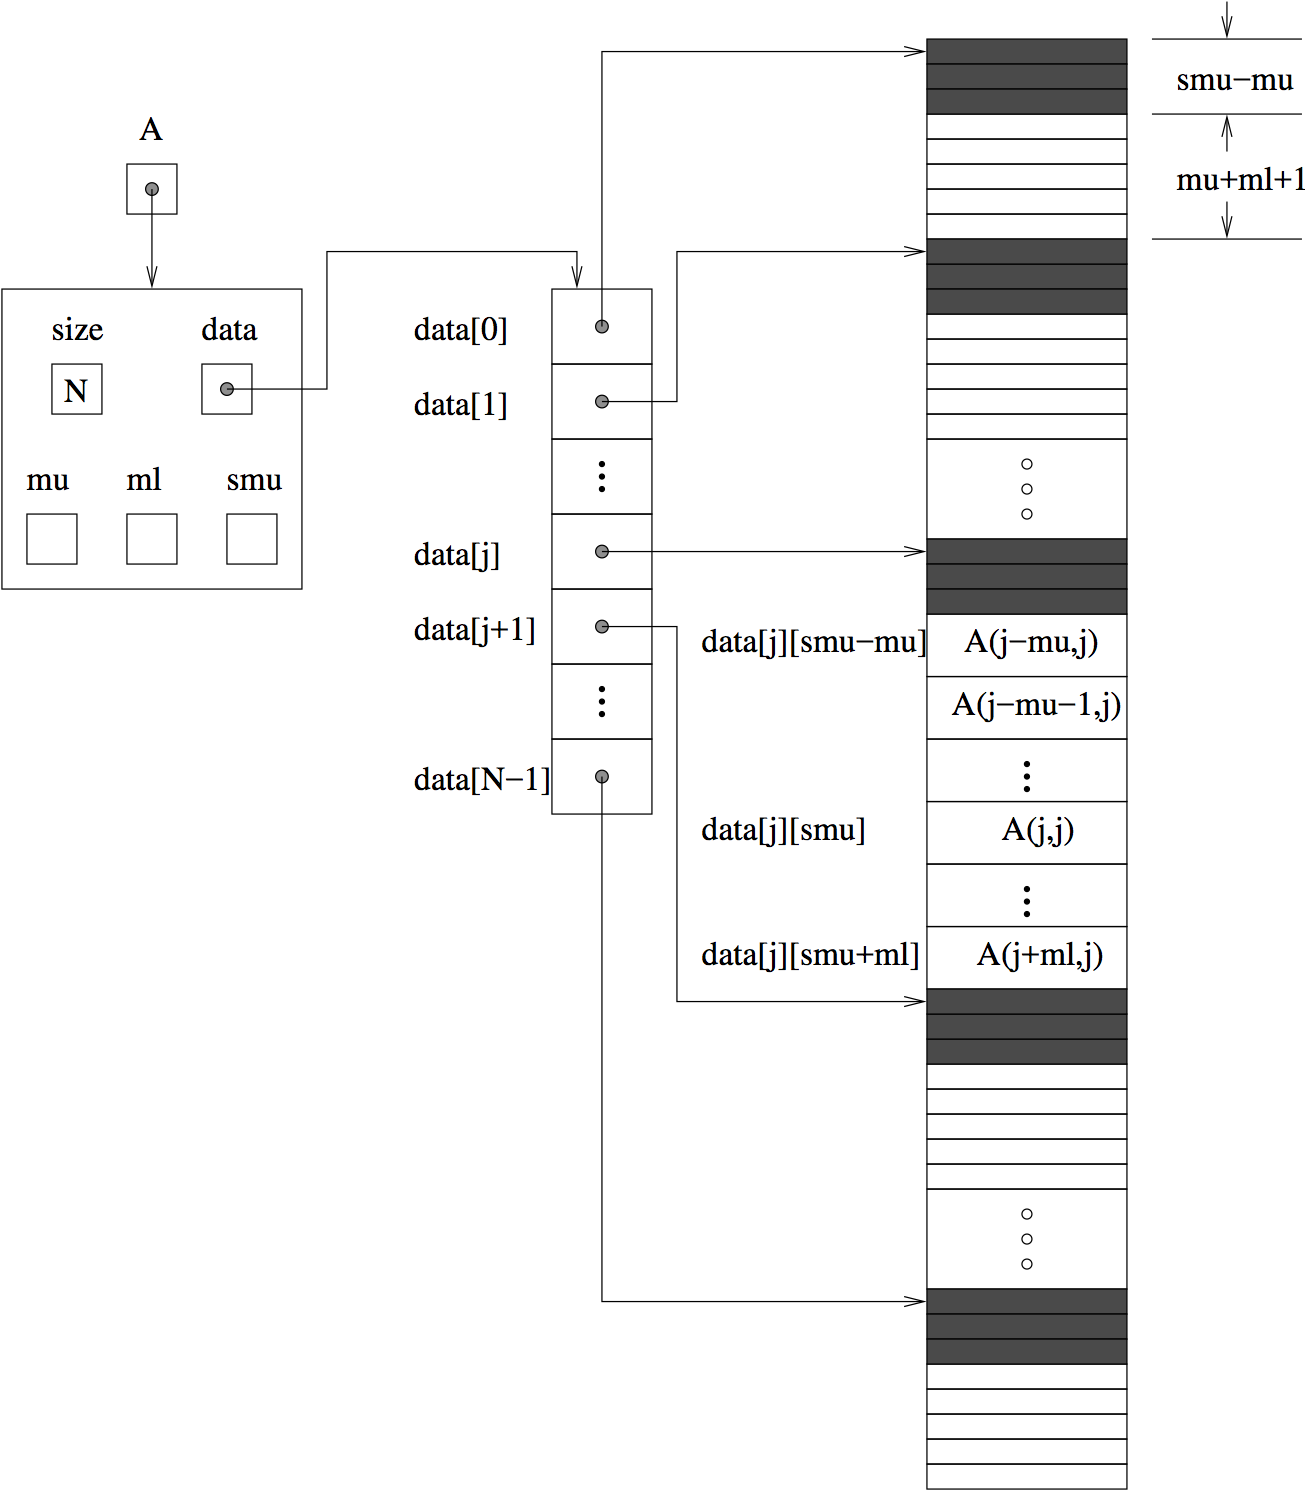
\includegraphics{bandmat1.png}
\caption{Diagram of the storage for the SUNMATRIX\_BAND module. Here \code{A} is an
\(N \times N\) band matrix with upper and lower half-bandwidths \code{mu}
and \code{ml}, respectively. The rows and columns of \code{A} are
numbered from 0 to \code{N-1} and the (\(i,j\))-th element of \code{A} is
denoted \code{A(i,j)}. The greyed out areas of the underlying
component storage are used by the associated SUNLINSOL\_BAND or
SUNLINSOL\_LAPACKBAND linear solver.}\label{sunmatrix/SUNMatrix_Band:sunbandmatrix}\end{figure}

The header file to be included when using this module is
\code{sunmatrix/sunmatrix\_band.h}.

The following macros are provided to access the
content of a SUNMATRIX\_BAND matrix. The prefix \code{SM\_} in the names
denotes that these macros are for \emph{SUNMatrix} implementations,
and the suffix \code{\_B} denotes that these are specific to
the \emph{banded} version.
\index{SM\_CONTENT\_B (C macro)}

\begin{fulllineitems}
\phantomsection\label{sunmatrix/SUNMatrix_Band:c.SM_CONTENT_B}\pysiglinewithargsret{\bfcode{SM\_CONTENT\_B}}{A}{}
This macro gives access to the contents of the banded \code{SUNMatrix} \emph{A}.

The assignment \code{A\_cont = SM\_CONTENT\_B(A)} sets
\code{A\_cont} to be a pointer to the banded \code{SUNMatrix} content
structure.

Implementation:

\begin{Verbatim}[commandchars=\\\{\}]
\PYG{c+cp}{\PYGZsh{}}\PYG{c+cp}{define SM\PYGZus{}CONTENT\PYGZus{}B(A)   ( (SUNMatrixContent\PYGZus{}Band)(A\PYGZhy{}\PYGZgt{}content) )}
\end{Verbatim}

\end{fulllineitems}

\index{SM\_ROWS\_B (C macro)}

\begin{fulllineitems}
\phantomsection\label{sunmatrix/SUNMatrix_Band:c.SM_ROWS_B}\pysiglinewithargsret{\bfcode{SM\_ROWS\_B}}{A}{}
Access the number of rows in the banded \code{SUNMatrix} \emph{A}.

This may be used either to retrieve or to set the value.  For
example, the assignment \code{A\_rows = SM\_ROWS\_B(A)} sets \code{A\_rows} to be
the number of rows in the matrix \code{A}.  Similarly, the
assignment \code{SM\_ROWS\_B(A) = A\_rows} sets the number of
columns in \code{A} to equal \code{A\_rows}.

Implementation:

\begin{Verbatim}[commandchars=\\\{\}]
\PYG{c+cp}{\PYGZsh{}}\PYG{c+cp}{define SM\PYGZus{}ROWS\PYGZus{}B(A)   ( SM\PYGZus{}CONTENT\PYGZus{}B(A)\PYGZhy{}\PYGZgt{}M )}
\end{Verbatim}

\end{fulllineitems}

\index{SM\_COLUMNS\_B (C macro)}

\begin{fulllineitems}
\phantomsection\label{sunmatrix/SUNMatrix_Band:c.SM_COLUMNS_B}\pysiglinewithargsret{\bfcode{SM\_COLUMNS\_B}}{A}{}
Access the number of columns in the banded \code{SUNMatrix} \emph{A}.  As
with \code{SM\_ROWS\_B}, this may be used either to retrieve or to set
the value.

Implementation:

\begin{Verbatim}[commandchars=\\\{\}]
\PYG{c+cp}{\PYGZsh{}}\PYG{c+cp}{define SM\PYGZus{}COLUMNS\PYGZus{}B(A)   ( SM\PYGZus{}CONTENT\PYGZus{}B(A)\PYGZhy{}\PYGZgt{}N )}
\end{Verbatim}

\end{fulllineitems}

\index{SM\_UBAND\_B (C macro)}

\begin{fulllineitems}
\phantomsection\label{sunmatrix/SUNMatrix_Band:c.SM_UBAND_B}\pysiglinewithargsret{\bfcode{SM\_UBAND\_B}}{A}{}
Access the \code{mu} parameter in the banded \code{SUNMatrix} \emph{A}.  As
with \code{SM\_ROWS\_B}, this may be used either to retrieve or to set
the value.

Implementation:

\begin{Verbatim}[commandchars=\\\{\}]
\PYG{c+cp}{\PYGZsh{}}\PYG{c+cp}{define SM\PYGZus{}UBAND\PYGZus{}B(A)   ( SM\PYGZus{}CONTENT\PYGZus{}B(A)\PYGZhy{}\PYGZgt{}mu )}
\end{Verbatim}

\end{fulllineitems}

\index{SM\_LBAND\_B (C macro)}

\begin{fulllineitems}
\phantomsection\label{sunmatrix/SUNMatrix_Band:c.SM_LBAND_B}\pysiglinewithargsret{\bfcode{SM\_LBAND\_B}}{A}{}
Access the \code{ml} parameter in the banded \code{SUNMatrix} \emph{A}.  As
with \code{SM\_ROWS\_B}, this may be used either to retrieve or to set
the value.

Implementation:

\begin{Verbatim}[commandchars=\\\{\}]
\PYG{c+cp}{\PYGZsh{}}\PYG{c+cp}{define SM\PYGZus{}LBAND\PYGZus{}B(A)   ( SM\PYGZus{}CONTENT\PYGZus{}B(A)\PYGZhy{}\PYGZgt{}ml )}
\end{Verbatim}

\end{fulllineitems}

\index{SM\_SUBAND\_B (C macro)}

\begin{fulllineitems}
\phantomsection\label{sunmatrix/SUNMatrix_Band:c.SM_SUBAND_B}\pysiglinewithargsret{\bfcode{SM\_SUBAND\_B}}{A}{}
Access the \code{smu} parameter in the banded \code{SUNMatrix} \emph{A}.  As
with \code{SM\_ROWS\_B}, this may be used either to retrieve or to set
the value.

Implementation:

\begin{Verbatim}[commandchars=\\\{\}]
\PYG{c+cp}{\PYGZsh{}}\PYG{c+cp}{define SM\PYGZus{}SUBAND\PYGZus{}B(A)   ( SM\PYGZus{}CONTENT\PYGZus{}B(A)\PYGZhy{}\PYGZgt{}smu )}
\end{Verbatim}

\end{fulllineitems}

\index{SM\_LDIM\_B (C macro)}

\begin{fulllineitems}
\phantomsection\label{sunmatrix/SUNMatrix_Band:c.SM_LDIM_B}\pysiglinewithargsret{\bfcode{SM\_LDIM\_B}}{A}{}
Access the \code{ldim} parameter in the banded \code{SUNMatrix} \emph{A}.  As
with \code{SM\_ROWS\_B}, this may be used either to retrieve or to set
the value.

Implementation:

\begin{Verbatim}[commandchars=\\\{\}]
\PYG{c+cp}{\PYGZsh{}}\PYG{c+cp}{define SM\PYGZus{}LDIM\PYGZus{}B(A)   ( SM\PYGZus{}CONTENT\PYGZus{}B(A)\PYGZhy{}\PYGZgt{}ldim )}
\end{Verbatim}

\end{fulllineitems}

\index{SM\_LDATA\_B (C macro)}

\begin{fulllineitems}
\phantomsection\label{sunmatrix/SUNMatrix_Band:c.SM_LDATA_B}\pysiglinewithargsret{\bfcode{SM\_LDATA\_B}}{A}{}
Access the \code{ldata} parameter in the banded \code{SUNMatrix} \emph{A}.  As
with \code{SM\_ROWS\_B}, this may be used either to retrieve or to set
the value.

Implementation:

\begin{Verbatim}[commandchars=\\\{\}]
\PYG{c+cp}{\PYGZsh{}}\PYG{c+cp}{define SM\PYGZus{}LDATA\PYGZus{}B(A)   ( SM\PYGZus{}CONTENT\PYGZus{}B(A)\PYGZhy{}\PYGZgt{}ldata )}
\end{Verbatim}

\end{fulllineitems}

\index{SM\_DATA\_B (C macro)}

\begin{fulllineitems}
\phantomsection\label{sunmatrix/SUNMatrix_Band:c.SM_DATA_B}\pysiglinewithargsret{\bfcode{SM\_DATA\_B}}{A}{}
This macro gives access to the \code{data} pointer for the matrix entries.

The assignment \code{A\_data = SM\_DATA\_B(A)} sets \code{A\_data} to be
a pointer to the first component of the data array for the banded
\code{SUNMatrix A}.  The assignment \code{SM\_DATA\_B(A) = A\_data}
sets the data array of \code{A} to be \code{A\_data} by storing the
pointer \code{A\_data}.

Implementation:

\begin{Verbatim}[commandchars=\\\{\}]
\PYG{c+cp}{\PYGZsh{}}\PYG{c+cp}{define SM\PYGZus{}DATA\PYGZus{}B(A)   ( SM\PYGZus{}CONTENT\PYGZus{}B(A)\PYGZhy{}\PYGZgt{}data )}
\end{Verbatim}

\end{fulllineitems}

\index{SM\_COLS\_B (C macro)}

\begin{fulllineitems}
\phantomsection\label{sunmatrix/SUNMatrix_Band:c.SM_COLS_B}\pysiglinewithargsret{\bfcode{SM\_COLS\_B}}{A}{}
This macro gives access to the \code{cols} pointer for the matrix entries.

The assignment \code{A\_cols = SM\_COLS\_B(A)} sets \code{A\_cols} to be
a pointer to the array of column pointers for the banded \code{SUNMatrix A}.
The assignment \code{SM\_COLS\_B(A) = A\_cols} sets the column pointer
array of \code{A} to be \code{A\_cols} by storing the pointer
\code{A\_cols}.

Implementation:

\begin{Verbatim}[commandchars=\\\{\}]
\PYG{c+cp}{\PYGZsh{}}\PYG{c+cp}{define SM\PYGZus{}COLS\PYGZus{}B(A)   ( SM\PYGZus{}CONTENT\PYGZus{}B(A)\PYGZhy{}\PYGZgt{}cols )}
\end{Verbatim}

\end{fulllineitems}

\index{SM\_COLUMN\_B (C macro)}

\begin{fulllineitems}
\phantomsection\label{sunmatrix/SUNMatrix_Band:c.SM_COLUMN_B}\pysiglinewithargsret{\bfcode{SM\_COLUMN\_B}}{A}{}
This macros gives access to the individual columns of the data
array of a banded \code{SUNMatrix}.

The assignment \code{col\_j = SM\_COLUMN\_B(A,j)} sets \code{col\_j} to be
a pointer to the diagonal element of the j-th column of the
\(N \times N\) band matrix \code{A}, \(0 \le j \le N-1\).
The type of the expression \code{SM\_COLUMN\_B(A,j)} is \code{realtype *}.
The pointer returned by the call \code{SM\_COLUMN\_B(A,j)} can be treated as
an array which is indexed from \code{-mu} to \code{ml}.

Implementation:

\begin{Verbatim}[commandchars=\\\{\}]
\PYG{c+cp}{\PYGZsh{}}\PYG{c+cp}{define SM\PYGZus{}COLUMN\PYGZus{}B(A,j)   ( ((SM\PYGZus{}CONTENT\PYGZus{}B(A)\PYGZhy{}\PYGZgt{}cols)[j])+SM\PYGZus{}SUBAND\PYGZus{}B(A) )}
\end{Verbatim}

\end{fulllineitems}

\index{SM\_ELEMENT\_B (C macro)}

\begin{fulllineitems}
\phantomsection\label{sunmatrix/SUNMatrix_Band:c.SM_ELEMENT_B}\pysiglinewithargsret{\bfcode{SM\_ELEMENT\_B}}{A}{}
This macro gives access to the individual entries of the data array
of a banded \code{SUNMatrix}.

The assignments \code{SM\_ELEMENT\_B(A,i,j) = a\_ij} and \code{a\_ij =
SM\_ELEMENT\_B(A,i,j)} reference the (\(i,j\))-th element of the
\(N \times N\) band matrix \code{A}, where \(0 \le i,j \le N-1\).
The location (\(i,j\)) should further satisfy
\(j-\text{mu} \le i \le j+\text{ml}\).

Implementation:

\begin{Verbatim}[commandchars=\\\{\}]
\PYG{c+cp}{\PYGZsh{}}\PYG{c+cp}{define SM\PYGZus{}ELEMENT\PYGZus{}B(A,i,j)   ( (SM\PYGZus{}CONTENT\PYGZus{}B(A)\PYGZhy{}\PYGZgt{}cols)[j][(i)\PYGZhy{}(j)+SM\PYGZus{}SUBAND\PYGZus{}B(A)] )}
\end{Verbatim}

\end{fulllineitems}

\index{SM\_COLUMN\_ELEMENT\_B (C macro)}

\begin{fulllineitems}
\phantomsection\label{sunmatrix/SUNMatrix_Band:c.SM_COLUMN_ELEMENT_B}\pysiglinewithargsret{\bfcode{SM\_COLUMN\_ELEMENT\_B}}{A}{}
This macro gives access to the individual entries of the data array
of a banded \code{SUNMatrix}.

The assignments \code{SM\_COLUMN\_ELEMENT\_B(col\_j,i,j) = a\_ij} and
\code{a\_ij = SM\_COLUMN\_ELEMENT\_B(col\_j,i,j)} reference the
(\(i,j\))-th entry of the band matrix \code{A} when used in
conjunction with \code{SM\_COLUMN\_B} to reference the j-th column
through \code{col\_j}. The index (\(i,j\)) should satisfy
\(j-\text{mu} \le i \le j+\text{ml}\).

Implementation:

\begin{Verbatim}[commandchars=\\\{\}]
\PYG{c+cp}{\PYGZsh{}}\PYG{c+cp}{define SM\PYGZus{}COLUMN\PYGZus{}ELEMENT\PYGZus{}B(col\PYGZus{}j,i,j)   (col\PYGZus{}j[(i)\PYGZhy{}(j)])}
\end{Verbatim}

\end{fulllineitems}


The SUNMATRIX\_BAND module defines banded implementations of all matrix
operations listed in the section {\hyperref[sunmatrix/SUNMatrix_Operations:sunmatrix-ops]{\emph{\DUspan{}{Description of the SUNMATRIX operations}}}}. Their names are
obtained from those in that section by appending the suffix \code{\_Band}
(e.g. \code{SUNMatCopy\_Band}).  The module SUNMATRIX\_BAND provides the
following additional user-callable routines:
\index{SUNBandMatrix (C function)}

\begin{fulllineitems}
\phantomsection\label{sunmatrix/SUNMatrix_Band:c.SUNBandMatrix}\pysiglinewithargsret{SUNMatrix \bfcode{SUNBandMatrix}}{sunindextype\emph{ N}, sunindextype\emph{ mu}, sunindextype\emph{ ml}}{}
This constructor function creates and allocates memory for a banded \code{SUNMatrix}.
Its arguments are the matrix size, \code{N}, and the upper and lower
half-bandwidths of the matrix, \code{mu} and \code{ml}.  The stored upper
bandwidth is set to \code{mu+ml} to accommodate subsequent
factorization in the SUNLINSOL\_BAND and SUNLINSOL\_LAPACKBAND
modules.

\end{fulllineitems}

\index{SUNBandMatrixStorage (C function)}

\begin{fulllineitems}
\phantomsection\label{sunmatrix/SUNMatrix_Band:c.SUNBandMatrixStorage}\pysiglinewithargsret{SUNMatrix \bfcode{SUNBandMatrixStorage}}{sunindextype\emph{ N}, sunindextype\emph{ mu}, sunindextype\emph{ ml}, sunindextype\emph{ smu}}{}
This constructor function creates and allocates memory for a banded \code{SUNMatrix}.
Its arguments are the matrix size, \code{N}, the upper and lower
half-bandwidths of the matrix, \code{mu} and \code{ml}, and the stored
upper bandwidth, \code{smu}.  When creating a band \code{SUNMatrix},
this value should be
\begin{itemize}
\item {} 
at least \code{min(N-1,mu+ml)} if the matrix will be
used by the SUNLinSol\_Band module;

\item {} 
exactly equal to \code{mu+ml} if the matrix will be used by
the SUNLinSol\_LapackBand module;

\item {} 
at least \code{mu} if used in some other manner.

\end{itemize}

\emph{Note: it is strongly recommended that users call the default
constructor, :c:func:{}`SUNBandMatrix(){}`, in all standard use cases.
This advanced constructor is used internally within SUNDIALS
solvers, and is provided to users who require banded matrices for
non-default purposes.}

\end{fulllineitems}

\index{SUNBandMatrix\_Print (C function)}

\begin{fulllineitems}
\phantomsection\label{sunmatrix/SUNMatrix_Band:c.SUNBandMatrix_Print}\pysiglinewithargsret{void \bfcode{SUNBandMatrix\_Print}}{SUNMatrix\emph{ A}, FILE*\emph{ outfile}}{}
This function prints the content of a banded \code{SUNMatrix} to the
output stream specified by \code{outfile}.  Note: \code{stdout}
or \code{stderr} may be used as arguments for \code{outfile} to print
directly to standard output or standard error, respectively.

\end{fulllineitems}

\index{SUNBandMatrix\_Rows (C function)}

\begin{fulllineitems}
\phantomsection\label{sunmatrix/SUNMatrix_Band:c.SUNBandMatrix_Rows}\pysiglinewithargsret{sunindextype \bfcode{SUNBandMatrix\_Rows}}{SUNMatrix\emph{ A}}{}
This function returns the number of rows in the banded \code{SUNMatrix}.

\end{fulllineitems}

\index{SUNBandMatrix\_Columns (C function)}

\begin{fulllineitems}
\phantomsection\label{sunmatrix/SUNMatrix_Band:c.SUNBandMatrix_Columns}\pysiglinewithargsret{sunindextype \bfcode{SUNBandMatrix\_Columns}}{SUNMatrix\emph{ A}}{}
This function returns the number of columns in the banded \code{SUNMatrix}.

\end{fulllineitems}

\index{SUNBandMatrix\_LowerBandwidth (C function)}

\begin{fulllineitems}
\phantomsection\label{sunmatrix/SUNMatrix_Band:c.SUNBandMatrix_LowerBandwidth}\pysiglinewithargsret{sunindextype \bfcode{SUNBandMatrix\_LowerBandwidth}}{SUNMatrix\emph{ A}}{}
This function returns the lower half-bandwidth for the banded \code{SUNMatrix}.

\end{fulllineitems}

\index{SUNBandMatrix\_UpperBandwidth (C function)}

\begin{fulllineitems}
\phantomsection\label{sunmatrix/SUNMatrix_Band:c.SUNBandMatrix_UpperBandwidth}\pysiglinewithargsret{sunindextype \bfcode{SUNBandMatrix\_UpperBandwidth}}{SUNMatrix\emph{ A}}{}
This function returns the upper half-bandwidth of the banded \code{SUNMatrix}.

\end{fulllineitems}

\index{SUNBandMatrix\_StoredUpperBandwidth (C function)}

\begin{fulllineitems}
\phantomsection\label{sunmatrix/SUNMatrix_Band:c.SUNBandMatrix_StoredUpperBandwidth}\pysiglinewithargsret{sunindextype \bfcode{SUNBandMatrix\_StoredUpperBandwidth}}{SUNMatrix\emph{ A}}{}
This function returns the stored upper half-bandwidth of the banded \code{SUNMatrix}.

\end{fulllineitems}

\index{SUNBandMatrix\_LDim (C function)}

\begin{fulllineitems}
\phantomsection\label{sunmatrix/SUNMatrix_Band:c.SUNBandMatrix_LDim}\pysiglinewithargsret{sunindextype \bfcode{SUNBandMatrix\_LDim}}{SUNMatrix\emph{ A}}{}
This function returns the length of the leading dimension of the banded \code{SUNMatrix}.

\end{fulllineitems}

\index{SUNBandMatrix\_Data (C function)}

\begin{fulllineitems}
\phantomsection\label{sunmatrix/SUNMatrix_Band:c.SUNBandMatrix_Data}\pysiglinewithargsret{realtype* \bfcode{SUNBandMatrix\_Data}}{SUNMatrix\emph{ A}}{}
This function returns a pointer to the data array for the banded \code{SUNMatrix}.

\end{fulllineitems}

\index{SUNBandMatrix\_Cols (C function)}

\begin{fulllineitems}
\phantomsection\label{sunmatrix/SUNMatrix_Band:c.SUNBandMatrix_Cols}\pysiglinewithargsret{realtype** \bfcode{SUNBandMatrix\_Cols}}{SUNMatrix\emph{ A}}{}
This function returns a pointer to the cols array for the band \code{SUNMatrix}.

\end{fulllineitems}

\index{SUNBandMatrix\_Column (C function)}

\begin{fulllineitems}
\phantomsection\label{sunmatrix/SUNMatrix_Band:c.SUNBandMatrix_Column}\pysiglinewithargsret{realtype* \bfcode{SUNBandMatrix\_Column}}{SUNMatrix\emph{ A}, sunindextype\emph{ j}}{}
This function returns a pointer to the diagonal entry of the j-th
column of the banded \code{SUNMatrix}.  The resulting pointer should
be indexed over the range \code{-mu} to \code{ml}.

\end{fulllineitems}


\textbf{Notes}
\begin{itemize}
\item {} 
When looping over the components of a banded \code{SUNMatrix A},
the most efficient approaches are to:
\begin{itemize}
\item {} 
First obtain the component array via \code{A\_data = SM\_DATA\_B(A)} or
\code{A\_data = SUNBandMatrix\_Data(A)} and then
access \code{A\_data{[}i{]}} within the loop.

\item {} 
First obtain the array of column pointers via \code{A\_cols = SM\_COLS\_B(A)} or
\code{A\_cols = SUNBandMatrix\_Cols(A)}, and then
access \code{A\_cols{[}j{]}{[}i{]}} within the loop.

\item {} 
Within a loop over the columns, access the column pointer via
\code{A\_colj = SUNBandMatrix\_Column(A,j)} and then to access the
entries within that column using \code{SM\_COLUMN\_ELEMENT\_B(A\_colj,i,j)}.

\end{itemize}

All three of these are more efficient than
using \code{SM\_ELEMENT\_B(A,i,j)} within a double loop.

\item {} 
Within the \code{SUNMatMatvec\_Band} routine, internal consistency
checks are performed to ensure that the matrix is called with
consistent \code{N\_Vector} implementations.  These are currently
limited to: NVECTOR\_SERIAL, NVECTOR\_OPENMP, and NVECTOR\_PTHREADS.
As additional compatible vector implementations are added to
SUNDIALS, these will be included within this compatibility check.

\end{itemize}

For solvers that include a Fortran interface module, the SUNMATRIX\_BAND
module also includes the Fortran-callable function
{\hyperref[sunmatrix/SUNMatrix_Band:f/_/FSUNBandMatInit]{\emph{\code{FSUNBandMatInit()}}}} to initialize this SUNMATRIX\_BAND module
for a given SUNDIALS solver.
\index{FSUNBandMatInit() (fortran subroutine)|textbf}

\begin{fulllineitems}
\phantomsection\label{sunmatrix/SUNMatrix_Band:f/_/FSUNBandMatInit}\pysiglinewithargsret{\strong{subroutine  }\bfcode{FSUNBandMatInit}}{\emph{CODE}, \emph{N}, \emph{MU}, \emph{ML}, \emph{IER}}{}
Initializes a band \code{SUNMatrix} structure for use in a SUNDIALS solver.
\begin{description}
\item[{\textbf{Arguments:}}] \leavevmode\begin{itemize}
\item {} 
\emph{CODE} (\code{int}, input) -- flag denoting the SUNDIALS solver
this matrix will be used for: CVODE=1, IDA=2, KINSOL=3, ARKode=4.

\item {} 
\emph{N} (\code{long int}, input) -- number of matrix rows (and columns).

\item {} 
\emph{MU} (\code{long int}, input) -- upper half-bandwidth.

\item {} 
\emph{ML} (\code{long int}, input) -- lower half-bandwidth.

\item {} 
\emph{IER} (\code{int}, output) -- return flag (0 success, -1 for failure).

\end{itemize}

\end{description}

\end{fulllineitems}


Additionally, when using ARKode with a non-identity mass matrix, the
Fortran-callable function {\hyperref[sunmatrix/SUNMatrix_Band:f/_/FSUNBandMassMatInit]{\emph{\code{FSUNBandMassMatInit()}}}} initializes
this SUNMATRIX\_BAND module for storing the mass matrix.
\index{FSUNBandMassMatInit() (fortran subroutine)|textbf}

\begin{fulllineitems}
\phantomsection\label{sunmatrix/SUNMatrix_Band:f/_/FSUNBandMassMatInit}\pysiglinewithargsret{\strong{subroutine  }\bfcode{FSUNBandMassMatInit}}{\emph{N}, \emph{MU}, \emph{ML}, \emph{IER}}{}
Initializes a band \code{SUNMatrix} structure for use as a mass
matrix in ARKode.
\begin{description}
\item[{\textbf{Arguments:}}] \leavevmode\begin{itemize}
\item {} 
\emph{N} (\code{long int}, input) -- number of matrix rows (and columns).

\item {} 
\emph{MU} (\code{long int}, input) -- upper half-bandwidth.

\item {} 
\emph{ML} (\code{long int}, input) -- lower half-bandwidth.

\item {} 
\emph{IER} (\code{int}, output) -- return flag (0 success, -1 for failure).

\end{itemize}

\end{description}

\end{fulllineitems}



\section{The SUNMATRIX\_SPARSE Module}
\label{sunmatrix/SUNMatrix_Sparse:sunmatrix-sparse}\label{sunmatrix/SUNMatrix_Sparse::doc}\label{sunmatrix/SUNMatrix_Sparse:the-sunmatrix-sparse-module}
The sparse implementation of the \code{SUNMatrix} module provided with
SUNDIALS, SUNMATRIX\_SPARSE, is designed to work with either
\emph{compressed-sparse-column} (CSC) or \emph{compressed-sparse-row}
(CSR) sparse matrix formats.  To this end, it defines the \emph{content}
field of \code{SUNMatrix} to be the following structure:

\begin{Verbatim}[commandchars=\\\{\}]
\PYG{k}{struct} \PYG{n}{\PYGZus{}SUNMatrixContent\PYGZus{}Sparse} \PYG{p}{\PYGZob{}}
  \PYG{n}{sunindextype} \PYG{n}{M}\PYG{p}{;}
  \PYG{n}{sunindextype} \PYG{n}{N}\PYG{p}{;}
  \PYG{n}{sunindextype} \PYG{n}{NNZ}\PYG{p}{;}
  \PYG{n}{sunindextype} \PYG{n}{NP}\PYG{p}{;}
  \PYG{n}{realtype} \PYG{o}{*}\PYG{n}{data}\PYG{p}{;}
  \PYG{k+kt}{int} \PYG{n}{sparsetype}\PYG{p}{;}
  \PYG{n}{sunindextype} \PYG{o}{*}\PYG{n}{indexvals}\PYG{p}{;}
  \PYG{n}{sunindextype} \PYG{o}{*}\PYG{n}{indexptrs}\PYG{p}{;}
  \PYG{c+cm}{/* CSC indices */}
  \PYG{n}{sunindextype} \PYG{o}{*}\PYG{o}{*}\PYG{n}{rowvals}\PYG{p}{;}
  \PYG{n}{sunindextype} \PYG{o}{*}\PYG{o}{*}\PYG{n}{colptrs}\PYG{p}{;}
  \PYG{c+cm}{/* CSR indices */}
  \PYG{n}{sunindextype} \PYG{o}{*}\PYG{o}{*}\PYG{n}{colvals}\PYG{p}{;}
  \PYG{n}{sunindextype} \PYG{o}{*}\PYG{o}{*}\PYG{n}{rowptrs}\PYG{p}{;}
\PYG{p}{\PYGZcb{}}\PYG{p}{;}
\end{Verbatim}

A diagram of the underlying data representation in a sparse matrix is
shown in Figure {\hyperref[sunmatrix/SUNMatrix_Sparse:sunsparsematrix]{\emph{\DUspan{}{SUNSparseMatrix Diagram}}}}.  A more
complete description of the parts of this \emph{content} field is given below:
\begin{itemize}
\item {} 
\code{M} - number of rows

\item {} 
\code{N} - number of columns

\item {} 
\code{NNZ} - maximum number of nonzero entries in the matrix
(allocated length of \code{data} and \code{indexvals} arrays)

\item {} 
\code{NP} - number of index pointers (e.g. number of column pointers
for CSC matrix). For CSC matrices \code{NP=N}, and for CSR matrices
\code{NP=M}. This value is set automatically at construction based the
input choice for \code{sparsetype}.

\item {} 
\code{data} - pointer to a contiguous block of \code{realtype}
variables (of length \code{NNZ}), containing the values of the
nonzero entries in the matrix

\item {} 
\code{sparsetype} - type of the sparse matrix (\code{CSC\_MAT} or \code{CSR\_MAT})

\item {} 
\code{indexvals} - pointer to a contiguous block of \code{int} variables
(of length \code{NNZ}), containing the row indices (if CSC) or column
indices (if CSR) of each nonzero matrix entry held in \code{data}

\item {} 
\code{indexptrs} - pointer to a contiguous block of \code{int}
variables (of length \code{NP+1}). For CSC matrices each entry provides
the index of the first column entry into the \code{data} and
\code{indexvals} arrays, e.g. if \code{indexptr{[}3{]}=7}, then the first
nonzero entry in the fourth column of the matrix is located in
\code{data{[}7{]}}, and is located in row \code{indexvals{[}7{]}} of the matrix.
The last entry contains the total number of nonzero values in the
matrix and hence points one past the end of the active data in the
\code{data} and \code{indexvals} arrays. For CSR matrices, each entry
provides the index of the first row entry into the \code{data} and
\code{indexvals} arrays.

\end{itemize}

The following pointers are added to the SUNMATRIX\_SPARSE content
structure for user convenience, to provide a more intuitive interface
to the CSC and CSR sparse matrix data structures. They are set
automatically when creating a sparse \code{SUNMatrix}, based on the
sparse matrix storage type.
\begin{itemize}
\item {} 
\code{rowvals} - pointer to \code{indexvals} when \code{sparsetype} is
\code{CSC\_MAT}, otherwise set to \code{NULL}.

\item {} 
\code{colptrs} - pointer to \code{indexptrs} when \code{sparsetype} is
\code{CSC\_MAT}, otherwise set to \code{NULL}.

\item {} 
\code{colvals} - pointer to \code{indexvals} when \code{sparsetype} is
\code{CSR\_MAT}, otherwise set to \code{NULL}.

\item {} 
\code{rowptrs} - pointer to \code{indexptrs} when \code{sparsetype} is
\code{CSR\_MAT}, otherwise set to \code{NULL}.

\end{itemize}

For example, the \(5\times 4\) matrix
\begin{gather}
\begin{split}\left[\begin{array}{cccc}
  0 & 3 & 1 & 0\\
  3 & 0 & 0 & 2\\
  0 & 7 & 0 & 0\\
  1 & 0 & 0 & 9\\
  0 & 0 & 0 & 5
\end{array}\right]\end{split}\notag
\end{gather}
could be stored as a CSC matrix in this structure as either

\begin{Verbatim}[commandchars=\\\{\}]
\PYG{n}{M} \PYG{o}{=} \PYG{l+m+mi}{5}\PYG{p}{;}
\PYG{n}{N} \PYG{o}{=} \PYG{l+m+mi}{4}\PYG{p}{;}
\PYG{n}{NNZ} \PYG{o}{=} \PYG{l+m+mi}{8}\PYG{p}{;}
\PYG{n}{NP} \PYG{o}{=} \PYG{n}{N}\PYG{p}{;}
\PYG{n}{data} \PYG{o}{=} \PYG{p}{\PYGZob{}}\PYG{l+m+mf}{3.0}\PYG{p}{,} \PYG{l+m+mf}{1.0}\PYG{p}{,} \PYG{l+m+mf}{3.0}\PYG{p}{,} \PYG{l+m+mf}{7.0}\PYG{p}{,} \PYG{l+m+mf}{1.0}\PYG{p}{,} \PYG{l+m+mf}{2.0}\PYG{p}{,} \PYG{l+m+mf}{9.0}\PYG{p}{,} \PYG{l+m+mf}{5.0}\PYG{p}{\PYGZcb{}}\PYG{p}{;}
\PYG{n}{sparsetype} \PYG{o}{=} \PYG{n}{CSC\PYGZus{}MAT}\PYG{p}{;}
\PYG{n}{indexvals} \PYG{o}{=} \PYG{p}{\PYGZob{}}\PYG{l+m+mi}{1}\PYG{p}{,} \PYG{l+m+mi}{3}\PYG{p}{,} \PYG{l+m+mi}{0}\PYG{p}{,} \PYG{l+m+mi}{2}\PYG{p}{,} \PYG{l+m+mi}{0}\PYG{p}{,} \PYG{l+m+mi}{1}\PYG{p}{,} \PYG{l+m+mi}{3}\PYG{p}{,} \PYG{l+m+mi}{4}\PYG{p}{\PYGZcb{}}\PYG{p}{;}
\PYG{n}{indexptrs} \PYG{o}{=} \PYG{p}{\PYGZob{}}\PYG{l+m+mi}{0}\PYG{p}{,} \PYG{l+m+mi}{2}\PYG{p}{,} \PYG{l+m+mi}{4}\PYG{p}{,} \PYG{l+m+mi}{5}\PYG{p}{,} \PYG{l+m+mi}{8}\PYG{p}{\PYGZcb{}}\PYG{p}{;}
\end{Verbatim}

or

\begin{Verbatim}[commandchars=\\\{\}]
\PYG{n}{M} \PYG{o}{=} \PYG{l+m+mi}{5}\PYG{p}{;}
\PYG{n}{N} \PYG{o}{=} \PYG{l+m+mi}{4}\PYG{p}{;}
\PYG{n}{NNZ} \PYG{o}{=} \PYG{l+m+mi}{10}\PYG{p}{;}
\PYG{n}{NP} \PYG{o}{=} \PYG{n}{N}\PYG{p}{;}
\PYG{n}{data} \PYG{o}{=} \PYG{p}{\PYGZob{}}\PYG{l+m+mf}{3.0}\PYG{p}{,} \PYG{l+m+mf}{1.0}\PYG{p}{,} \PYG{l+m+mf}{3.0}\PYG{p}{,} \PYG{l+m+mf}{7.0}\PYG{p}{,} \PYG{l+m+mf}{1.0}\PYG{p}{,} \PYG{l+m+mf}{2.0}\PYG{p}{,} \PYG{l+m+mf}{9.0}\PYG{p}{,} \PYG{l+m+mf}{5.0}\PYG{p}{,} \PYG{o}{*}\PYG{p}{,} \PYG{o}{*}\PYG{p}{\PYGZcb{}}\PYG{p}{;}
\PYG{n}{sparsetype} \PYG{o}{=} \PYG{n}{CSC\PYGZus{}MAT}\PYG{p}{;}
\PYG{n}{indexvals} \PYG{o}{=} \PYG{p}{\PYGZob{}}\PYG{l+m+mi}{1}\PYG{p}{,} \PYG{l+m+mi}{3}\PYG{p}{,} \PYG{l+m+mi}{0}\PYG{p}{,} \PYG{l+m+mi}{2}\PYG{p}{,} \PYG{l+m+mi}{0}\PYG{p}{,} \PYG{l+m+mi}{1}\PYG{p}{,} \PYG{l+m+mi}{3}\PYG{p}{,} \PYG{l+m+mi}{4}\PYG{p}{,} \PYG{o}{*}\PYG{p}{,} \PYG{o}{*}\PYG{p}{\PYGZcb{}}\PYG{p}{;}
\PYG{n}{indexptrs} \PYG{o}{=} \PYG{p}{\PYGZob{}}\PYG{l+m+mi}{0}\PYG{p}{,} \PYG{l+m+mi}{2}\PYG{p}{,} \PYG{l+m+mi}{4}\PYG{p}{,} \PYG{l+m+mi}{5}\PYG{p}{,} \PYG{l+m+mi}{8}\PYG{p}{\PYGZcb{}}\PYG{p}{;}
\end{Verbatim}

where the first has no unused space, and the second has additional
storage (the entries marked with \code{*} may contain any values).
Note in both cases that the final value in \code{indexptrs} is 8,
indicating the total number of nonzero entries in the matrix.

Similarly, in CSR format, the same matrix could be stored as

\begin{Verbatim}[commandchars=\\\{\}]
\PYG{n}{M} \PYG{o}{=} \PYG{l+m+mi}{5}\PYG{p}{;}
\PYG{n}{N} \PYG{o}{=} \PYG{l+m+mi}{4}\PYG{p}{;}
\PYG{n}{NNZ} \PYG{o}{=} \PYG{l+m+mi}{8}\PYG{p}{;}
\PYG{n}{NP} \PYG{o}{=} \PYG{n}{N}\PYG{p}{;}
\PYG{n}{data} \PYG{o}{=} \PYG{p}{\PYGZob{}}\PYG{l+m+mf}{3.0}\PYG{p}{,} \PYG{l+m+mf}{1.0}\PYG{p}{,} \PYG{l+m+mf}{3.0}\PYG{p}{,} \PYG{l+m+mf}{2.0}\PYG{p}{,} \PYG{l+m+mf}{7.0}\PYG{p}{,} \PYG{l+m+mf}{1.0}\PYG{p}{,} \PYG{l+m+mf}{9.0}\PYG{p}{,} \PYG{l+m+mf}{5.0}\PYG{p}{\PYGZcb{}}\PYG{p}{;}
\PYG{n}{sparsetype} \PYG{o}{=} \PYG{n}{CSR\PYGZus{}MAT}\PYG{p}{;}
\PYG{n}{indexvals} \PYG{o}{=} \PYG{p}{\PYGZob{}}\PYG{l+m+mi}{1}\PYG{p}{,} \PYG{l+m+mi}{2}\PYG{p}{,} \PYG{l+m+mi}{0}\PYG{p}{,} \PYG{l+m+mi}{3}\PYG{p}{,} \PYG{l+m+mi}{1}\PYG{p}{,} \PYG{l+m+mi}{0}\PYG{p}{,} \PYG{l+m+mi}{3}\PYG{p}{,} \PYG{l+m+mi}{3}\PYG{p}{\PYGZcb{}}\PYG{p}{;}
\PYG{n}{indexptrs} \PYG{o}{=} \PYG{p}{\PYGZob{}}\PYG{l+m+mi}{0}\PYG{p}{,} \PYG{l+m+mi}{2}\PYG{p}{,} \PYG{l+m+mi}{4}\PYG{p}{,} \PYG{l+m+mi}{5}\PYG{p}{,} \PYG{l+m+mi}{7}\PYG{p}{,} \PYG{l+m+mi}{8}\PYG{p}{\PYGZcb{}}\PYG{p}{;}
\end{Verbatim}
\begin{figure}[htbp]
\centering
\capstart

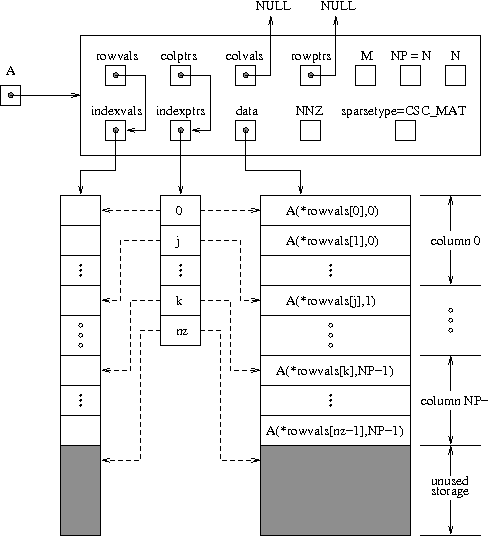
\includegraphics{cscmat1.png}
\caption{Diagram of the storage for a compressed-sparse-column matrix of
type SUNMATRIX\_SPARSE: Here \code{A} is an \(M \times N\) sparse
CSC matrix with storage for up to \code{NNZ} nonzero entries (the
allocated length of both \code{data} and \code{indexvals}).  The entries
in \code{indexvals} may assume values from \code{0} to \code{M-1},
corresponding to the row index (zero-based) of
each nonzero value.  The entries in \code{data} contain the values of
the nonzero entries, with the row \code{i}, column \code{j} entry of
\code{A} (again, zero-based) denoted as \code{A(i,j)}.  The \code{indexptrs}
array contains \code{N+1} entries; the first \code{N} denote the starting
index of each column within the \code{indexvals} and \code{data} arrays,
while the final entry points one past the final nonzero entry.
Here, although \code{NNZ} values are allocated, only \code{nz} are
actually filled in; the greyed-out portions of \code{data} and
\code{indexvals} indicate extra allocated space.}\label{sunmatrix/SUNMatrix_Sparse:sunsparsematrix}\end{figure}

The header file to be included when using this module is
\code{sunmatrix/sunmatrix\_sparse.h}.

The following macros are provided to access the content of a
SUNMATRIX\_SPARSE matrix. The prefix \code{SM\_} in the names
denotes that these macros are for \emph{SUNMatrix} implementations,
and the suffix \code{\_S} denotes that these are specific to
the \emph{sparse} version.
\index{SM\_CONTENT\_S (C macro)}

\begin{fulllineitems}
\phantomsection\label{sunmatrix/SUNMatrix_Sparse:c.SM_CONTENT_S}\pysiglinewithargsret{\bfcode{SM\_CONTENT\_S}}{A}{}
This macro gives access to the contents of the sparse \code{SUNMatrix} \emph{A}.

The assignment \code{A\_cont = SM\_CONTENT\_S(A)} sets
\code{A\_cont} to be a pointer to the sparse \code{SUNMatrix} content
structure.

Implementation:

\begin{Verbatim}[commandchars=\\\{\}]
\PYG{c+cp}{\PYGZsh{}}\PYG{c+cp}{define SM\PYGZus{}CONTENT\PYGZus{}S(A)   ( (SUNMatrixContent\PYGZus{}Sparse)(A\PYGZhy{}\PYGZgt{}content) )}
\end{Verbatim}

\end{fulllineitems}

\index{SM\_ROWS\_S (C macro)}

\begin{fulllineitems}
\phantomsection\label{sunmatrix/SUNMatrix_Sparse:c.SM_ROWS_S}\pysiglinewithargsret{\bfcode{SM\_ROWS\_S}}{A}{}
Access the number of rows in the sparse \code{SUNMatrix} \emph{A}.

This may be used either to retrieve or to set the value.  For
example, the assignment \code{A\_rows = SM\_ROWS\_S(A)} sets \code{A\_rows}
to be the number of rows in the matrix \emph{A}.  Similarly, the
assignment \code{SM\_ROWS\_S(A) = A\_rows} sets the number of
columns in \emph{A} to equal \code{A\_rows}.

Implementation:

\begin{Verbatim}[commandchars=\\\{\}]
\PYG{c+cp}{\PYGZsh{}}\PYG{c+cp}{define SM\PYGZus{}ROWS\PYGZus{}S(A)   ( SM\PYGZus{}CONTENT\PYGZus{}S(A)\PYGZhy{}\PYGZgt{}M )}
\end{Verbatim}

\end{fulllineitems}

\index{SM\_COLUMNS\_S (C macro)}

\begin{fulllineitems}
\phantomsection\label{sunmatrix/SUNMatrix_Sparse:c.SM_COLUMNS_S}\pysiglinewithargsret{\bfcode{SM\_COLUMNS\_S}}{A}{}
Access the number of columns in the sparse \code{SUNMatrix} \emph{A}.  As
with \code{SM\_ROWS\_S}, this may be used either to retrieve or to set
the value.

Implementation:

\begin{Verbatim}[commandchars=\\\{\}]
\PYG{c+cp}{\PYGZsh{}}\PYG{c+cp}{define SM\PYGZus{}COLUMNS\PYGZus{}S(A)   ( SM\PYGZus{}CONTENT\PYGZus{}S(A)\PYGZhy{}\PYGZgt{}N )}
\end{Verbatim}

\end{fulllineitems}

\index{SM\_NNZ\_S (C macro)}

\begin{fulllineitems}
\phantomsection\label{sunmatrix/SUNMatrix_Sparse:c.SM_NNZ_S}\pysiglinewithargsret{\bfcode{SM\_NNZ\_S}}{A}{}
Access the allocated number of nonzeros in the sparse \code{SUNMatrix}
\emph{A}.  As with \code{SM\_ROWS\_S}, this may be used either to retrieve or
to set the value.

Implementation:

\begin{Verbatim}[commandchars=\\\{\}]
\PYG{c+cp}{\PYGZsh{}}\PYG{c+cp}{define SM\PYGZus{}NNZ\PYGZus{}S(A)   ( SM\PYGZus{}CONTENT\PYGZus{}S(A)\PYGZhy{}\PYGZgt{}NNZ )}
\end{Verbatim}

\end{fulllineitems}

\index{SM\_NP\_S (C macro)}

\begin{fulllineitems}
\phantomsection\label{sunmatrix/SUNMatrix_Sparse:c.SM_NP_S}\pysiglinewithargsret{\bfcode{SM\_NP\_S}}{A}{}
Access the number of index pointers \code{NP} in the sparse
\code{SUNMatrix} \emph{A}.  As with \code{SM\_ROWS\_S}, this may be used either
to retrieve or to set the value.

Implementation:

\begin{Verbatim}[commandchars=\\\{\}]
\PYG{c+cp}{\PYGZsh{}}\PYG{c+cp}{define SM\PYGZus{}NP\PYGZus{}S(A)   ( SM\PYGZus{}CONTENT\PYGZus{}S(A)\PYGZhy{}\PYGZgt{}NP )}
\end{Verbatim}

\end{fulllineitems}

\index{SM\_SPARSETYPE\_S (C macro)}

\begin{fulllineitems}
\phantomsection\label{sunmatrix/SUNMatrix_Sparse:c.SM_SPARSETYPE_S}\pysiglinewithargsret{\bfcode{SM\_SPARSETYPE\_S}}{A}{}
Access the sparsity type parameter in the sparse \code{SUNMatrix} \emph{A}.
As with \code{SM\_ROWS\_S}, this may be used either to retrieve or to
set the value.

Implementation:

\begin{Verbatim}[commandchars=\\\{\}]
\PYG{c+cp}{\PYGZsh{}}\PYG{c+cp}{define SM\PYGZus{}SPARSETYPE\PYGZus{}S(A)   ( SM\PYGZus{}CONTENT\PYGZus{}S(A)\PYGZhy{}\PYGZgt{}sparsetype )}
\end{Verbatim}

\end{fulllineitems}

\index{SM\_DATA\_S (C macro)}

\begin{fulllineitems}
\phantomsection\label{sunmatrix/SUNMatrix_Sparse:c.SM_DATA_S}\pysiglinewithargsret{\bfcode{SM\_DATA\_S}}{A}{}
This macro gives access to the \code{data} pointer for the matrix
entries.

The assignment \code{A\_data = SM\_DATA\_S(A)} sets \code{A\_data} to be
a pointer to the first component of the data array for the sparse
\code{SUNMatrix A}.  The assignment \code{SM\_DATA\_S(A) = A\_data}
sets the data array of \emph{A} to be \code{A\_data} by storing the
pointer \code{A\_data}.

Implementation:

\begin{Verbatim}[commandchars=\\\{\}]
\PYG{c+cp}{\PYGZsh{}}\PYG{c+cp}{define SM\PYGZus{}DATA\PYGZus{}S(A)   ( SM\PYGZus{}CONTENT\PYGZus{}S(A)\PYGZhy{}\PYGZgt{}data )}
\end{Verbatim}

\end{fulllineitems}

\index{SM\_INDEXVALS\_S (C macro)}

\begin{fulllineitems}
\phantomsection\label{sunmatrix/SUNMatrix_Sparse:c.SM_INDEXVALS_S}\pysiglinewithargsret{\bfcode{SM\_INDEXVALS\_S}}{A}{}
This macro gives access to the \code{indexvals} pointer for the matrix
entries.

The assignment \code{A\_indexvals = SM\_INDEXVALS\_S(A)}
sets \code{A\_indexvals} to be a pointer to the array of index values
(i.e. row indices for a CSC matrix, or column indices for a CSR
matrix) for the sparse \code{SUNMatrix} \emph{A}.

Implementation:

\begin{Verbatim}[commandchars=\\\{\}]
\PYG{c+cp}{\PYGZsh{}}\PYG{c+cp}{define SM\PYGZus{}INDEXVALS\PYGZus{}S(A)   ( SM\PYGZus{}CONTENT\PYGZus{}S(A)\PYGZhy{}\PYGZgt{}indexvals )}
\end{Verbatim}

\end{fulllineitems}

\index{SM\_INDEXPTRS\_S (C macro)}

\begin{fulllineitems}
\phantomsection\label{sunmatrix/SUNMatrix_Sparse:c.SM_INDEXPTRS_S}\pysiglinewithargsret{\bfcode{SM\_INDEXPTRS\_S}}{A}{}
This macro gives access to the \code{indexptrs} pointer for the matrix entries.

The assignment \code{A\_indexptrs = SM\_INDEXPTRS\_S(A)}
sets \code{A\_indexptrs} to be a pointer to the array of index
pointers (i.e. the starting indices in the data/indexvals arrays for
each row or column in CSR or CSC formats, respectively).

Implementation:

\begin{Verbatim}[commandchars=\\\{\}]
\PYG{c+cp}{\PYGZsh{}}\PYG{c+cp}{define SM\PYGZus{}INDEXPTRS\PYGZus{}S(A)   ( SM\PYGZus{}CONTENT\PYGZus{}S(A)\PYGZhy{}\PYGZgt{}indexptrs )}
\end{Verbatim}

\end{fulllineitems}


The SUNMATRIX\_SPARSE module defines sparse implementations of all matrix
operations listed in the section {\hyperref[sunmatrix/SUNMatrix_Operations:sunmatrix-ops]{\emph{\DUspan{}{Description of the SUNMATRIX operations}}}}. Their names are
obtained from those in that section by appending the suffix \code{\_Sparse}
(e.g. \code{SUNMatCopy\_Sparse}).  The module SUNMATRIX\_SPARSE provides the
following additional user-callable routines:
\index{SUNSparseMatrix (C function)}

\begin{fulllineitems}
\phantomsection\label{sunmatrix/SUNMatrix_Sparse:c.SUNSparseMatrix}\pysiglinewithargsret{SUNMatrix \bfcode{SUNSparseMatrix}}{sunindextype\emph{ M}, sunindextype\emph{ N}, sunindextype\emph{ NNZ}, int\emph{ sparsetype}}{}
This constructor function creates and allocates memory for a sparse
\code{SUNMatrix}.  Its arguments are the number of rows and columns of
the matrix, \emph{M} and \emph{N}, the maximum number of nonzeros to be
stored in the matrix, \emph{NNZ}, and a flag \emph{sparsetype} indicating
whether to use CSR or CSC format (valid choices are \code{CSR\_MAT} or
\code{CSC\_MAT}).

\end{fulllineitems}

\index{SUNSparseFromDenseMatrix (C function)}

\begin{fulllineitems}
\phantomsection\label{sunmatrix/SUNMatrix_Sparse:c.SUNSparseFromDenseMatrix}\pysiglinewithargsret{SUNMatrix \bfcode{SUNSparseFromDenseMatrix}}{SUNMatrix\emph{ A}, realtype\emph{ droptol}, int\emph{ sparsetype}}{}
This constructor function creates a new sparse matrix from an
existing SUNMATRIX\_DENSE object by copying all values with
magnitude larger than \emph{droptol} into the sparse matrix structure.

Requirements:
\begin{itemize}
\item {} 
\emph{A} must have type \code{SUNMATRIX\_DENSE}

\item {} 
\emph{droptol} must be non-negative

\item {} 
\emph{sparsetype} must be either \code{CSC\_MAT} or \code{CSR\_MAT}

\end{itemize}

The function returns \code{NULL} if any requirements are violated, or if
the matrix storage request cannot be satisfied.

\end{fulllineitems}

\index{SUNSparseFromBandMatrix (C function)}

\begin{fulllineitems}
\phantomsection\label{sunmatrix/SUNMatrix_Sparse:c.SUNSparseFromBandMatrix}\pysiglinewithargsret{SUNMatrix \bfcode{SUNSparseFromBandMatrix}}{SUNMatrix\emph{ A}, realtype\emph{ droptol}, int\emph{ sparsetype}}{}
This constructor function creates a new sparse matrix from an
existing SUNMATRIX\_BAND object by copying all values with
magnitude larger than \emph{droptol} into the sparse matrix structure.

Requirements:
\begin{itemize}
\item {} 
\emph{A} must have type \code{SUNMATRIX\_BAND}

\item {} 
\emph{droptol} must be non-negative

\item {} 
\emph{sparsetype} must be either \code{CSC\_MAT} or \code{CSR\_MAT}.

\end{itemize}

The function returns \code{NULL} if any requirements are violated, or if
the matrix storage request cannot be satisfied.

\end{fulllineitems}

\index{SUNSparseMatrix\_Realloc (C function)}

\begin{fulllineitems}
\phantomsection\label{sunmatrix/SUNMatrix_Sparse:c.SUNSparseMatrix_Realloc}\pysiglinewithargsret{int \bfcode{SUNSparseMatrix\_Realloc}}{SUNMatrix\emph{ A}}{}
This function reallocates internal storage arrays in a sparse matrix
so that the resulting sparse matrix has no wasted space (i.e. the
space allocated for nonzero entries equals the actual number of
nonzeros, \code{indexptrs{[}NP{]}}). Returns 0 on success and
1 on failure (e.g. if the input matrix is not sparse).

\end{fulllineitems}

\index{SUNSparseMatrix\_Print (C function)}

\begin{fulllineitems}
\phantomsection\label{sunmatrix/SUNMatrix_Sparse:c.SUNSparseMatrix_Print}\pysiglinewithargsret{void \bfcode{SUNSparseMatrix\_Print}}{SUNMatrix\emph{ A}, FILE*\emph{ outfile}}{}
This function prints the content of a sparse \code{SUNMatrix} to the
output stream specified by \code{outfile}.  Note: \code{stdout}
or \code{stderr} may be used as arguments for \code{outfile} to print
directly to standard output or standard error, respectively.

\end{fulllineitems}

\index{SUNSparseMatrix\_Rows (C function)}

\begin{fulllineitems}
\phantomsection\label{sunmatrix/SUNMatrix_Sparse:c.SUNSparseMatrix_Rows}\pysiglinewithargsret{sunindextype \bfcode{SUNSparseMatrix\_Rows}}{SUNMatrix\emph{ A}}{}
This function returns the number of rows in the sparse \code{SUNMatrix}.

\end{fulllineitems}

\index{SUNSparseMatrix\_Columns (C function)}

\begin{fulllineitems}
\phantomsection\label{sunmatrix/SUNMatrix_Sparse:c.SUNSparseMatrix_Columns}\pysiglinewithargsret{sunindextype \bfcode{SUNSparseMatrix\_Columns}}{SUNMatrix\emph{ A}}{}
This function returns the number of columns in the sparse \code{SUNMatrix}.

\end{fulllineitems}

\index{SUNSparseMatrix\_NNZ (C function)}

\begin{fulllineitems}
\phantomsection\label{sunmatrix/SUNMatrix_Sparse:c.SUNSparseMatrix_NNZ}\pysiglinewithargsret{sunindextype \bfcode{SUNSparseMatrix\_NNZ}}{SUNMatrix\emph{ A}}{}
This function returns the number of entries allocated for nonzero
storage for the sparse \code{SUNMatrix}.

\end{fulllineitems}

\index{SUNSparseMatrix\_NP (C function)}

\begin{fulllineitems}
\phantomsection\label{sunmatrix/SUNMatrix_Sparse:c.SUNSparseMatrix_NP}\pysiglinewithargsret{sunindextype \bfcode{SUNSparseMatrix\_NP}}{SUNMatrix\emph{ A}}{}
This function returns the number of index pointers for the
sparse \code{SUNMatrix} (the \code{indexptrs} array has \code{NP+1}
entries).

\end{fulllineitems}

\index{SUNSparseMatrix\_SparseType (C function)}

\begin{fulllineitems}
\phantomsection\label{sunmatrix/SUNMatrix_Sparse:c.SUNSparseMatrix_SparseType}\pysiglinewithargsret{int \bfcode{SUNSparseMatrix\_SparseType}}{SUNMatrix\emph{ A}}{}
This function returns the storage type (\code{CSR\_MAT}
or \code{CSC\_MAT}) for the sparse  \code{SUNMatrix}.

\end{fulllineitems}

\index{SUNSparseMatrix\_Data (C function)}

\begin{fulllineitems}
\phantomsection\label{sunmatrix/SUNMatrix_Sparse:c.SUNSparseMatrix_Data}\pysiglinewithargsret{realtype* \bfcode{SUNSparseMatrix\_Data}}{SUNMatrix\emph{ A}}{}
This function returns a pointer to the data array for the
sparse \code{SUNMatrix}.

\end{fulllineitems}

\index{SUNSparseMatrix\_IndexValues (C function)}

\begin{fulllineitems}
\phantomsection\label{sunmatrix/SUNMatrix_Sparse:c.SUNSparseMatrix_IndexValues}\pysiglinewithargsret{sunindextype* \bfcode{SUNSparseMatrix\_IndexValues}}{SUNMatrix\emph{ A}}{}
This function returns a pointer to index value array for the sparse
\code{SUNMatrix}: for CSR format this is the column index for each nonzero
entry, for CSC format this is the row index for each nonzero entry.

\end{fulllineitems}

\index{SUNSparseMatrix\_IndexPointers (C function)}

\begin{fulllineitems}
\phantomsection\label{sunmatrix/SUNMatrix_Sparse:c.SUNSparseMatrix_IndexPointers}\pysiglinewithargsret{sunindextype* \bfcode{SUNSparseMatrix\_IndexPointers}}{SUNMatrix\emph{ A}}{}
This function returns a pointer to the index pointer array for the
sparse \code{SUNMatrix}: for CSR format this is the location of the first
entry of each row in the \code{data} and \code{indexvalues} arrays, for
CSC format this is the location of the first entry of each column.

\end{fulllineitems}


\begin{notice}{note}{Note:}
Within the \code{SUNMatMatvec\_Sparse} routine, internal
consistency checks are performed to ensure that the matrix
is called with consistent \code{N\_Vector} implementations.
These are currently limited to: NVECTOR\_SERIAL,
NVECTOR\_OPENMP, NVECTOR\_PTHREADS, and NVECTOR\_CUDA when using
managed memory. As additional compatible vector implementations
are added to SUNDIALS, these will be included within this
compatibility check.
\end{notice}

For solvers that include a Fortran interface module, the SUNMATRIX\_SPARSE
module also includes the Fortran-callable function
{\hyperref[sunmatrix/SUNMatrix_Sparse:f/_/FSUNSparseMatInit]{\emph{\code{FSUNSparseMatInit()}}}} to initialize this SUNMATRIX\_SPARSE module
for a given SUNDIALS solver.
\index{FSUNSparseMatInit() (fortran subroutine)|textbf}

\begin{fulllineitems}
\phantomsection\label{sunmatrix/SUNMatrix_Sparse:f/_/FSUNSparseMatInit}\pysiglinewithargsret{\strong{subroutine  }\bfcode{FSUNSparseMatInit}}{\emph{CODE}, \emph{M}, \emph{N}, \emph{NNZ}, \emph{SPARSETYPE}, \emph{IER}}{}
Initializes a sparse \code{SUNMatrix} structure for use in a SUNDIALS solver.
\begin{description}
\item[{\textbf{Arguments:}}] \leavevmode\begin{itemize}
\item {} 
\emph{CODE} (\code{int}, input) -- flag denoting the SUNDIALS solver
this matrix will be used for: CVODE=1, IDA=2, KINSOL=3, ARKode=4.

\item {} 
\emph{M} (\code{long int}, input) -- number of matrix rows.

\item {} 
\emph{N} (\code{long int}, input) -- number of matrix columns.

\item {} 
\emph{NNZ} (\code{long int}, input) -- amount of nonzero storage to allocate.

\item {} 
\emph{SPARSETYPE} (\code{int}, input) -- matrix sparsity type
(\code{CSC\_MAT} or \code{CSR\_MAT})

\item {} 
\emph{IER} (\code{int}, output) -- return flag (0 success, -1 for failure).

\end{itemize}

\end{description}

\end{fulllineitems}


Additionally, when using ARKode with a non-identity mass matrix, the
Fortran-callable function {\hyperref[sunmatrix/SUNMatrix_Sparse:f/_/FSUNSparseMassMatInit]{\emph{\code{FSUNSparseMassMatInit()}}}} initializes
this SUNMATRIX\_SPARSE module for storing the mass matrix.
\index{FSUNSparseMassMatInit() (fortran subroutine)|textbf}

\begin{fulllineitems}
\phantomsection\label{sunmatrix/SUNMatrix_Sparse:f/_/FSUNSparseMassMatInit}\pysiglinewithargsret{\strong{subroutine  }\bfcode{FSUNSparseMassMatInit}}{\emph{M}, \emph{N}, \emph{NNZ}, \emph{SPARSETYPE}, \emph{IER}}{}
Initializes a sparse \code{SUNMatrix} structure for use as a mass
matrix in ARKode.
\begin{description}
\item[{\textbf{Arguments:}}] \leavevmode\begin{itemize}
\item {} 
\emph{M} (\code{long int}, input) -- number of matrix rows.

\item {} 
\emph{N} (\code{long int}, input) -- number of matrix columns.

\item {} 
\emph{NNZ} (\code{long int}, input) -- amount of nonzero storage to allocate.

\item {} 
\emph{SPARSETYPE} (\code{int}, input) -- matrix sparsity type
(\code{CSC\_MAT} or \code{CSR\_MAT})

\item {} 
\emph{IER} (\code{int}, output) -- return flag (0 success, -1 for failure).

\end{itemize}

\end{description}

\end{fulllineitems}



\section{The SUNMATRIX\_SLUNRLOC Module}
\label{sunmatrix/SUNMatrix_SLUNRloc:sunmatrix-slunrloc}\label{sunmatrix/SUNMatrix_SLUNRloc:the-sunmatrix-slunrloc-module}\label{sunmatrix/SUNMatrix_SLUNRloc::doc}
The SUNMATRIX\_SLUNRLOC implementation of the SUNMatrix module provided
with SUNDIALS is an adapter for the \code{SuperMatrix} structure provided by
the SuperLU\_DIST sparse matrix factorization and solver library written
by X. Sherry Li (\phantomsection\label{sunmatrix/SUNMatrix_SLUNRloc:id1}{\hyperref[References:superludist]{\emph{{[}SuperLUDIST{]}}}}, \phantomsection\label{sunmatrix/SUNMatrix_SLUNRloc:id2}{\hyperref[References:gdl2007]{\emph{{[}GDL2007{]}}}}, \phantomsection\label{sunmatrix/SUNMatrix_SLUNRloc:id3}{\hyperref[References:ld2003]{\emph{{[}LD2003{]}}}}, \phantomsection\label{sunmatrix/SUNMatrix_SLUNRloc:id4}{\hyperref[References:sluug1999]{\emph{{[}SLUUG1999{]}}}}).
It is designed to be used with the SuperLU\_DIST \code{SUNLinearSolver}
discussed in Section {\hyperref[sunlinsol/SUNLinSol_SuperLUDIST:sunlinsol-superludist]{\emph{\DUspan{}{The SUNLinSol\_SuperLUDIST Module}}}}. To this end, it defines
the \code{content} field of \code{SUNMatrix} to be the following structure:

\begin{Verbatim}[commandchars=\\\{\}]
\PYG{k}{struct} \PYG{n}{\PYGZus{}SUNMatrixContent\PYGZus{}SLUNRloc} \PYG{p}{\PYGZob{}}
  \PYG{n}{booleantype}   \PYG{n}{own\PYGZus{}data}\PYG{p}{;}
  \PYG{n}{gridinfo\PYGZus{}t}    \PYG{o}{*}\PYG{n}{grid}\PYG{p}{;}
  \PYG{n}{sunindextype}  \PYG{o}{*}\PYG{n}{row\PYGZus{}to\PYGZus{}proc}\PYG{p}{;}
  \PYG{n}{pdgsmv\PYGZus{}comm\PYGZus{}t} \PYG{o}{*}\PYG{n}{gsmv\PYGZus{}comm}\PYG{p}{;}
  \PYG{n}{SuperMatrix}   \PYG{o}{*}\PYG{n}{A\PYGZus{}super}\PYG{p}{;}
  \PYG{n}{SuperMatrix}   \PYG{o}{*}\PYG{n}{ACS\PYGZus{}super}\PYG{p}{;}
\PYG{p}{\PYGZcb{}}\PYG{p}{;}
\end{Verbatim}

A more complete description of the this \code{content} field is given below:
\begin{itemize}
\item {} 
\code{own\_data} -- a flag which indicates if the SUNMatrix is responsible for freeing
\code{A\_super}

\item {} 
\code{grid} -- pointer to the SuperLU\_DIST structure that stores the 2D process grid

\item {} 
\code{row\_to\_proc} -- a mapping between the rows in the matrix and the process it
resides on; will be \code{NULL} until the \code{SUNMatMatvecSetup} routine is called

\item {} 
\code{gsmv\_comm} -- pointer to the SuperLU\_DIST structure that stores the
communication information needed for matrix-vector multiplication; will be
\code{NULL} until the \code{SUNMatMatvecSetup} routine is called

\item {} \begin{description}
\item[{\code{A\_super} -- pointer to the underlying SuperLU\_DIST \code{SuperMatrix} with}] \leavevmode
\code{Stype = SLU\_NR\_loc, Dtype = SLU\_D, Mtype = SLU\_GE}; must have the
full diagonal present to be used with \code{SUNMatScaleAddI} routine

\end{description}

\item {} 
\code{ACS\_super} -- a column-sorted version of the matrix needed to perform matrix-vector
multiplication; will be \code{NULL} until the routine \code{SUNMatMatvecSetup}
routine is called

\end{itemize}

The header file to include when using this module is \code{sunmatrix/sunmatrix\_slunrloc.h}.
The installed module library to link to is \code{libsundials\_sunmatrixslunrloc} \emph{.lib}
where \emph{.lib} is typically \code{.so} for shared libraries and \code{.a} for static libraries.


\subsection{SUNMATRIX\_SLUNRLOC Functions}
\label{sunmatrix/SUNMatrix_SLUNRloc:sunmatrix-slunrloc-functions}\label{sunmatrix/SUNMatrix_SLUNRloc:id5}
The SUNMATRIX\_SLUNRLOC module provides the following user-callable routines:
\index{SUNMatrix\_SLUNRloc (C function)}

\begin{fulllineitems}
\phantomsection\label{sunmatrix/SUNMatrix_SLUNRloc:c.SUNMatrix_SLUNRloc}\pysiglinewithargsret{SUNMatrix \bfcode{SUNMatrix\_SLUNRloc}}{SuperMatrix\emph{ *Asuper}, gridinfo\_t\emph{ *grid}}{}
This constructor function creates and allocates memory for a SUNMatrix\_SLUNRloc
object. Its arguments are a fully-allocated SuperLU\_DIST \code{SuperMatrix} with
\code{Stype = SLU\_NR\_loc, Dtype = SLU\_D, Mtype = SLU\_GE} and an initialized SuperLU\_DIST
2D process grid structure. It returns a SUNMatrix object if \code{Asuper} is compatible
else it returns \code{NULL}.

\end{fulllineitems}

\index{SUNMatrix\_SLUNRloc\_Print (C function)}

\begin{fulllineitems}
\phantomsection\label{sunmatrix/SUNMatrix_SLUNRloc:c.SUNMatrix_SLUNRloc_Print}\pysiglinewithargsret{void \bfcode{SUNMatrix\_SLUNRloc\_Print}}{SUNMatrix\emph{ A}, FILE\emph{ *fp}}{}
This function prints the underlying \code{SuperMatrix} content. It is useful for
debugging. Its arguments are the \code{SUNMatrix} object and a \code{FILE} pointer
to print to. It returns void.

\end{fulllineitems}

\index{SUNMatrix\_SLUNRloc\_SuperMatrix (C function)}

\begin{fulllineitems}
\phantomsection\label{sunmatrix/SUNMatrix_SLUNRloc:c.SUNMatrix_SLUNRloc_SuperMatrix}\pysiglinewithargsret{SuperMatrix* \bfcode{SUNMatrix\_SLUNRloc\_SuperMatrix}}{SUNMatrix\emph{ A}}{}
This function returns the underlying \code{SuperMatrix} of \code{A}. Its
only argument is the \code{SUNMatrix} object to access.

\end{fulllineitems}

\index{SUNMatrix\_SLUNRloc\_ProcessGrid (C function)}

\begin{fulllineitems}
\phantomsection\label{sunmatrix/SUNMatrix_SLUNRloc:c.SUNMatrix_SLUNRloc_ProcessGrid}\pysiglinewithargsret{gridinfo\_t* \bfcode{SUNMatrix\_SLUNRloc\_ProcessGrid}}{SUNMatrix\emph{ A}}{}
This function returns the SuperLU\_DIST 2D process grid associated with
\code{A}. Its only argument is the \code{SUNMatrix} object to access.

\end{fulllineitems}

\index{SUNMatrix\_SLUNRloc\_OwnData (C function)}

\begin{fulllineitems}
\phantomsection\label{sunmatrix/SUNMatrix_SLUNRloc:c.SUNMatrix_SLUNRloc_OwnData}\pysiglinewithargsret{booleantype \bfcode{SUNMatrix\_SLUNRloc\_OwnData}}{SUNMatrix\emph{ A}}{}
This function returns true if the \code{SUNMatrix} object is responsible
for freeing the underlying \code{SuperMatrix}, otherwise it returns false.
Its only argument is the \code{SUNMatrix} object to access.

\end{fulllineitems}


The SUNMATRIX\_SLUNRLOC module also defines implementations of all generic
\code{SUNMatrix} operations listed in Table {\hyperref[sunmatrix/SUNMatrix_Operations:sunmatrix-ops]{\emph{\DUspan{}{Description of the SUNMATRIX operations}}}}:
\begin{itemize}
\item {} 
\code{SUNMatGetID\_SLUNRloc} -- returns \code{SUNMATRIX\_SLUNRLOC}

\item {} 
\code{SUNMatClone\_SLUNRloc}

\item {} 
\code{SUNMatDestroy\_SLUNRloc}

\item {} 
\code{SUNMatSpace\_SLUNRloc} -- this only returns information for the storage within
the matrix interface, i.e. storage for \code{row\_to\_proc}

\item {} 
\code{SUNMatZero\_SLUNRloc}

\item {} 
\code{SUNMatCopy\_SLUNRloc}

\item {} \begin{description}
\item[{\code{SUNMatScaleAdd\_SLUNRloc} -- performs \(A = cA + B\), where \(A\) and \(B\)}] \leavevmode
must have the same sparsity pattern

\end{description}

\item {} 
\code{SUNMatScaleAddI\_SLUNRloc} -- performs \(A = cA + I\), where the diagonal of \(A\)
must be present

\item {} 
\code{SUNMatMatvecSetup\_SLUNRloc} -- initializes the SuperLU\_DIST parallel communication
structures needed to perform a matrix-vector product; only needs to be called before
the first call to \code{SUNMatMatvec} or if the matrix changed since the last setup

\item {} 
\code{SUNMatMatvec\_SLUNRloc}

\end{itemize}


\section{SUNMATRIX Examples}
\label{sunmatrix/SUNMatrix_Examples::doc}\label{sunmatrix/SUNMatrix_Examples:sunmatrix-examples}\label{sunmatrix/SUNMatrix_Examples:id1}
There are \code{SUNMatrix} examples that may be installed for each
implementation: dense, banded, and sparse.  Each implementation
makes use of the functions in \code{test\_sunmatrix.c}.
These example functions show simple usage of the \code{SUNMatrix} family
of functions.  The inputs to the examples depend on the matrix type,
and are output to \code{stdout} if the example is run without the
appropriate number of command-line arguments.

The following is a list of the example functions in \code{test\_sunmatrix.c}:
\begin{itemize}
\item {} 
\code{Test\_SUNMatGetID}: Verifies the returned matrix ID against
the value that should be returned.

\item {} 
\code{Test\_SUNMatClone}: Creates clone of an existing matrix,
copies the data, and checks that their values match.

\item {} 
\code{Test\_SUNMatZero}: Zeros out an existing matrix and checks
that each entry equals 0.0.

\item {} 
\code{Test\_SUNMatCopy}: Clones an input matrix, copies its data
to a clone, and verifies that all values match.

\item {} 
\code{Test\_SUNMatScaleAdd}: Given an input matrix \(A\) and an
input identity matrix \(I\), this test clones and copies
\(A\) to a new matrix \(B\), computes \(B = -B+B\), and
verifies that the resulting matrix entries equal 0.  Additionally,
if the matrix is square, this test clones and copies \(A\) to a
new matrix \(D\), clones and copies \(I\) to a new matrix
\(C\), computes \(D = D+I\) and \(C = C+A\) using
\code{SUNMatScaleAdd}, and then verifies that \(C=D\).

\item {} 
\code{Test\_SUNMatScaleAddI}: Given an input matrix \(A\) and an
input identity matrix \(I\), this clones and copies \(I\) to
a new matrix \(B\), computes \(B = -B+I\) using
\code{SUNMatScaleAddI}, and verifies that the resulting matrix entries
equal 0.

\item {} 
\code{Test\_SUNMatMatvec} Given an input matrix \(A\) and input
vectors \(x\) and \(y\) such that \(y=Ax\), this test
has different behavior depending on whether \(A\) is square.  If
it is square, it clones and copies \(A\) to a new matrix
\(B\), computes \(B = 3B+I\) using \code{SUNMatScaleAddI},
clones \(y\) to new vectors \(w\) and \(z\), computes
\(z = Bx\) using \code{SUNMatMatvec}, computes \(w = 3y+x\)
using \code{N\_VLinearSum}, and verifies that \(w==z\).  If
\(A\) is not square, it just clones \(y\) to a new vector
\(z\), \emph{computes :math:{}`z=Ax} using \code{SUNMatMatvec}, and
verifies that \(y=z\).

\item {} 
\code{Test\_SUNMatSpace}: verifies that \code{SUNMatSpace} can be
called, and outputs the results to \code{stdout}.

\end{itemize}


\section{SUNMATRIX functions required by ARKode}
\label{sunmatrix/ARKode_requirements:sunmatrix-arkode}\label{sunmatrix/ARKode_requirements:sunmatrix-functions-required-by-arkode}\label{sunmatrix/ARKode_requirements::doc}
In Table {\hyperref[sunmatrix/ARKode_requirements:sunmatrix-arkode-use]{\emph{\DUspan{}{List of matrix functions usage by ARKode code modules}}}}, we list the matrix functions in
the \code{SUNMatrix} module used within the ARKode package.  The table
also shows, for each function, which of the code modules uses the
function.  The main ARKode time step modules, ARKStep and ERKStep, do
not call any \code{SUNMatrix} functions directly, so the table columns
are specific to the ARKLS interface and the ARKBANDPRE and ARKBBDPRE
preconditioner modules.   We further note that the ARKLS interface
only utilizes these routines when supplied with a \emph{matrix-based}
linear solver, i.e. the \code{SUNMatrix} object (\emph{J} or \emph{M}) passed to
{\hyperref[ARKStep_c_interface/User_callable:c.ARKStepSetLinearSolver]{\emph{\code{ARKStepSetLinearSolver()}}}} or
{\hyperref[ARKStep_c_interface/User_callable:c.ARKStepSetMassLinearSolver]{\emph{\code{ARKStepSetMassLinearSolver()}}}} was not \code{NULL}.

At this point, we should emphasize that the ARKode user does not need
to know anything about the usage of matrix functions by the ARKode
code modules in order to use ARKode.  The information is presented as
an implementation detail for the interested reader.


\subsection{List of matrix functions usage by ARKode code modules}
\label{sunmatrix/ARKode_requirements:list-of-matrix-functions-usage-by-arkode-code-modules}\label{sunmatrix/ARKode_requirements:sunmatrix-arkode-use}
\begin{tabulary}{\linewidth}{|L|L|L|L|}
\hline
\textsf{\relax 
Routine
} & \textsf{\relax 
ARKLS
} & \textsf{\relax 
ARKBANDPRE
} & \textsf{\relax 
ARKBBDPRE
}\\
\hline
SUNMatGetID
 & 
X
 &  & \\
\hline
SUNMatClone
 & 
X
 &  & \\
\hline
SUNMatDestroy
 & 
X
 & 
X
 & 
X
\\
\hline
SUNMatZero
 & 
X
 & 
X
 & 
X
\\
\hline
SUNMatCopy
 & 
X
 & 
X
 & 
X
\\
\hline
SUNMatScaleAddI
 & 
X
 & 
X
 & 
X
\\
\hline
SUNMatScaleAdd
 & 
1
 &  & \\
\hline
SUNMatMatvec
 & 
1
 &  & \\
\hline
SUNMatMatvecSetup
 & 
1,2
 &  & \\
\hline
SUNMatSpace
 & 
2
 & 
2
 & 
2
\\
\hline\end{tabulary}

\begin{enumerate}
\item {} 
These matrix functions are only used for problems involving a
non-identity mass matrix.

\item {} 
These matrix functions are optionally used, in that these are only
called if they are implemented in the \code{SUNMatrix} module that is
being used (i.e. their function pointers are non-\code{NULL}).  If not
supplied, these modules will assume that the matrix requires no
storage.

\end{enumerate}

We note that both the ARKBANDPRE and ARKBBDPRE preconditioner modules
are hard-coded to use the SUNDIALS-supplied band \code{SUNMatrix} type,
so the most useful information above for user-supplied \code{SUNMatrix}
implementations is the column relating to ARKLS requirements.


\chapter{Description of the SUNLinearSolver module}
\label{sunlinsol/index::doc}\label{sunlinsol/index:sunlinsol}\label{sunlinsol/index:description-of-the-sunlinearsolver-module}
For problems that require the solution of linear systems of equations,
the SUNDIALS packages operate using generic linear solver modules
defined through the SUNLinSol API.  This allows SUNDIALS
packages to utilize any valid SUNLinSol implementation that provides
a set of required functions.  These functions can be divided into
three categories.  The first are the core linear solver functions.  The
second group consists of ``set'' routines to supply the linear solver object
with functions provided by the SUNDIALS package, or for modification
of solver parameters.  The last group consists of ``get'' routines for
retrieving artifacts (statistics, residual vectors, etc.) from the
linear solver.  All of these functions are defined in the header file
\code{sundials/sundials\_linearsolver.h}.

The implementations provided with SUNDIALS work in coordination
with the SUNDIALS generic \code{N\_Vector} and \code{SUNMatrix} modules to
provide a set of compatible data structures and solvers for the
solution of linear systems using direct or iterative (matrix-based or matrix-free)
methods. Moreover, advanced users can provide a customized
\code{SUNLinearSolver} implementation to any SUNDIALS package,
particularly in cases where they provide their own \code{N\_Vector} and/or
\code{SUNMatrix} modules.

Historically, the SUNDIALS packages have been designed to specifically
leverage the use of either \emph{direct linear solvers} or matrix-free,
\emph{scaled, preconditioned, iterative linear solvers}.  However,
matrix-based iterative linear solvers are also supported.

The iterative linear solvers packaged with SUNDIALS leverage scaling
and preconditioning, as applicable, to balance error between solution
components and to accelerate convergence of the linear solver.  To
this end, instead of solving the linear system \(Ax = b\)
directly, these apply the underlying iterative algorithm to the
transformed system
\phantomsection\label{sunlinsol/index:equation-eq:transformed_linear_system}\begin{gather}
\begin{split}\tilde{A} \tilde{x} = \tilde{b}\end{split}\label{sunlinsol/index-eq:transformed_linear_system}
\end{gather}
where
\phantomsection\label{sunlinsol/index:equation-eq:transformed_linear_system_components}\begin{gather}
\begin{split}\tilde{A} &= S_1 P_1^{-1} A P_2^{-1} S_2^{-1},\\
\tilde{b} &= S_1 P_1^{-1} b,\\
\tilde{x} &= S_2 P_2 x,\end{split}\label{sunlinsol/index-eq:transformed_linear_system_components}
\end{gather}
and where
\begin{itemize}
\item {} 
\(P_1\) is the left preconditioner,

\item {} 
\(P_2\) is the right preconditioner,

\item {} 
\(S_1\) is a diagonal matrix of scale factors for
\(P_1^{-1} b\),

\item {} 
\(S_2\) is a diagonal matrix of scale factors for \(P_2 x\).

\end{itemize}

SUNDIALS solvers request that iterative linear solvers stop
based on the 2-norm of the scaled preconditioned residual meeting a
prescribed tolerance
\begin{gather}
\begin{split}\left\| \tilde{b} - \tilde{A} \tilde{x} \right\|_2  <  \text{tol}.\end{split}\notag
\end{gather}
When provided an iterative SUNLinSol implementation that does not
support the scaling matrices \(S_1\) and \(S_2\), SUNDIALS'
packages will adjust the value of \(\text{tol}\) accordingly
(see the section {\hyperref[sunlinsol/ARKode_requirements:sunlinsol-iterative-tolerance]{\emph{\DUspan{}{Iterative linear solver tolerance}}}} for more details).  In
this case, they instead request that iterative linear solvers stop
based on the criteria
\begin{gather}
\begin{split}\left\| P_1^{-1} b - P_1^{-1} A x \right\|_2  <  \text{tol}.\end{split}\notag
\end{gather}
We note that the corresponding adjustments to \(\text{tol}\) in
this case are non-optimal, in that they cannot balance error between
specific entries of the solution \(x\), only the aggregate error
in the overall solution vector.

We further note that not all of the SUNDIALS-provided iterative linear
solvers support the full range of the above options (e.g., separate
left/right preconditioning), and that some of the SUNDIALS packages
only utilize a subset of these options.  Further details on these
exceptions are described in the documentation for each
\code{SUNLinearSolver} implementation, or for each SUNDIALS package.

For users interested in providing their own SUNLinSol module, the
following section presents the SUNLinSol API and its implementation
beginning with the definition of SUNLinSol functions in sections
{\hyperref[sunlinsol/SUNLinSol_API:sunlinsol-corefn]{\emph{\DUspan{}{SUNLinearSolver core functions}}}} -- {\hyperref[sunlinsol/SUNLinSol_API:sunlinsol-getfn]{\emph{\DUspan{}{SUNLinearSolver get functions}}}}. This is followed by
the definition of functions supplied to a linear solver implementation in
section {\hyperref[sunlinsol/SUNLinSol_API:sunlinsol-sunsuppliedfn]{\emph{\DUspan{}{Functions provided by SUNDIALS packages}}}}. The linear solver return
codes are described in section {\hyperref[sunlinsol/SUNLinSol_API:sunlinsol-errorcodes]{\emph{\DUspan{}{SUNLinearSolver return codes}}}}. The
\code{SUNLinearSolver} type and the generic SUNLinSol module are defined
in section {\hyperref[sunlinsol/SUNLinSol_API:sunlininsol-generic]{\emph{\DUspan{}{The generic SUNLinearSolver module}}}}.  The section
{\hyperref[sunlinsol/SUNLinSol_API:sunlinsol-compatibility]{\emph{\DUspan{}{Compatibility of SUNLinearSolver modules}}}} discusses compatibility between the
SUNDIALS-provided SUNLinSol modules and SUNMATRIX modules.  Section
{\hyperref[sunlinsol/SUNLinSol_API:sunlinsol-custom]{\emph{\DUspan{}{Implementing a custom SUNLinearSolver module}}}} lists the requirements for supplying a
custom SUNLinSol module and discusses some intended use cases. Users wishing to
supply their own SUNLinSol module are encouraged to use the SUNLinSol
implementations provided with SUNDIALS as a template for supplying custom
linear solver modules. The SUNLinSol functions required by this SUNDIALS
package as well as other package specific details are given in
section {\hyperref[sunlinsol/ARKode_requirements:sunlinsol-arkode]{\emph{\DUspan{}{ARKode SUNLinearSolver interface}}}}. The remaining sections of this chapter
present the SUNLinSol modules provided with SUNDIALS.


\section{The SUNLinearSolver API}
\label{sunlinsol/SUNLinSol_API::doc}\label{sunlinsol/SUNLinSol_API:sunlinsol-api}\label{sunlinsol/SUNLinSol_API:the-sunlinearsolver-api}
The SUNLinSol API defines several linear solver operations that enable
SUNDIALS packages to utilize any SUNLinSol implementation that
provides the required functions. These functions can be divided into
three categories. The first are the core linear solver functions. The
second group of functions consists of set routines to supply the
linear solver with functions provided by the SUNDIALS time integrators
and to modify solver parameters. The final group consists of get
routines for retrieving linear solver statistics. All of these
functions are defined in the header file
\code{sundials/sundials\_linearsolver.h}.


\subsection{SUNLinearSolver core functions}
\label{sunlinsol/SUNLinSol_API:sunlinsol-corefn}\label{sunlinsol/SUNLinSol_API:sunlinearsolver-core-functions}
The core linear solver functions consist of two required functions to get the
linear solver type ({\hyperref[sunlinsol/SUNLinSol_API:c.SUNLinSolGetType]{\emph{\code{SUNLinSolGetType()}}}}) and solve the linear system
\(Ax=b\) ({\hyperref[sunlinsol/SUNLinSol_API:c.SUNLinSolSolve]{\emph{\code{SUNLinSolSolve()}}}}). The remaining functions are for
getting the solver ID ({\hyperref[sunlinsol/SUNLinSol_API:c.SUNLinSolGetID]{\emph{\code{SUNLinSolGetID()}}}}), initializing the linear solver
object once all solver-specific options have been set
({\hyperref[sunlinsol/SUNLinSol_API:c.SUNLinSolInitialize]{\emph{\code{SUNLinSolInitialize()}}}}), setting up the linear solver object to utilize
an updated matrix \(A\) ({\hyperref[sunlinsol/SUNLinSol_API:c.SUNLinSolSetup]{\emph{\code{SUNLinSolSetup()}}}}), and for destroying the
linear solver object ({\hyperref[sunlinsol/SUNLinSol_API:c.SUNLinSolFree]{\emph{\code{SUNLinSolFree()}}}}) are optional.
\index{SUNLinSolGetType (C function)}

\begin{fulllineitems}
\phantomsection\label{sunlinsol/SUNLinSol_API:c.SUNLinSolGetType}\pysiglinewithargsret{SUNLinearSolver\_Type \bfcode{SUNLinSolGetType}}{SUNLinearSolver\emph{ LS}}{}
Returns the type identifier for the linear solver \emph{LS}. It is used to
determine the solver type (direct, iterative, or matrix-iterative) from
the abstract \code{SUNLinearSolver} interface.  Returned values are
one of the following:
\begin{itemize}
\item {} 
\code{SUNLINEARSOLVER\_DIRECT} -- \code{0}, the SUNLinSol module
requires a matrix, and computes an `exact' solution to the linear
system defined by that matrix.

\item {} 
\code{SUNLINEARSOLVER\_ITERATIVE} -- \code{1}, the SUNLinSol module does
not require a matrix (though one may be provided), and computes
an inexact solution to the linear system using a matrix-free
iterative algorithm. That is it solves the linear system defined
by the package-supplied \code{ATimes} routine (see
{\hyperref[sunlinsol/SUNLinSol_API:c.SUNLinSolSetATimes]{\emph{\code{SUNLinSolSetATimes()}}}} below), even if that linear system
differs from the one encoded in the matrix object (if one is
provided). As the solver computes the solution only inexactly (or
may diverge), the linear solver should check for solution
convergence/accuracy as appropriate.

\item {} 
\code{SUNLINEARSOLVER\_MATRIX\_ITERATIVE} -- \code{2}, the SUNLinSol
module requires a matrix, and computes an inexact solution to the
linear system defined by that matrix using an iterative
algorithm. That is it solves the linear system defined by the
matrix object even if that linear system differs from that
encoded by the package-supplied \code{ATimes} routine. As the solver
computes the solution only inexactly (or may diverge), the linear
solver should check for solution convergence/accuracy as
appropriate.

\end{itemize}

Usage:

\begin{Verbatim}[commandchars=\\\{\}]
\PYG{n}{type} \PYG{o}{=} \PYG{n}{SUNLinSolGetType}\PYG{p}{(}\PYG{n}{LS}\PYG{p}{)}\PYG{p}{;}
\end{Verbatim}

Notes: See section {\hyperref[sunlinsol/SUNLinSol_API:sunlinsol-intended]{\emph{\DUspan{}{Intended use cases}}}} for more information
on intended use cases corresponding to the linear solver type.

\end{fulllineitems}

\index{SUNLinSolGetID (C function)}

\begin{fulllineitems}
\phantomsection\label{sunlinsol/SUNLinSol_API:c.SUNLinSolGetID}\pysiglinewithargsret{SUNLinearSolver\_ID \bfcode{SUNLinSolGetID}}{SUNLinearSolver\emph{ LS}}{}
Returns the identifier for the linear solver \emph{LS}. It is recommended that a
user-supplied \code{SUNLinearSolver} implementation return the
\code{SUNLINEARSOLVER\_CUSTOM} identifier.

Usage:

\begin{Verbatim}[commandchars=\\\{\}]
\PYG{n}{id} \PYG{o}{=} \PYG{n}{SUNLinSolGetID}\PYG{p}{(}\PYG{n}{LS}\PYG{p}{)}\PYG{p}{;}
\end{Verbatim}

\end{fulllineitems}

\index{SUNLinSolInitialize (C function)}

\begin{fulllineitems}
\phantomsection\label{sunlinsol/SUNLinSol_API:c.SUNLinSolInitialize}\pysiglinewithargsret{int \bfcode{SUNLinSolInitialize}}{SUNLinearSolver\emph{ LS}}{}
Performs linear solver initialization (assuming that all
solver-specific options have been set).  This should return zero for a
successful call, and a negative value for a failure, ideally
returning one of the generic error codes listed in section
{\hyperref[sunlinsol/SUNLinSol_API:sunlinsol-errorcodes]{\emph{\DUspan{}{SUNLinearSolver return codes}}}}.

Usage:

\begin{Verbatim}[commandchars=\\\{\}]
\PYG{n}{retval} \PYG{o}{=} \PYG{n}{SUNLinSolInitialize}\PYG{p}{(}\PYG{n}{LS}\PYG{p}{)}\PYG{p}{;}
\end{Verbatim}

\end{fulllineitems}

\index{SUNLinSolSetup (C function)}

\begin{fulllineitems}
\phantomsection\label{sunlinsol/SUNLinSol_API:c.SUNLinSolSetup}\pysiglinewithargsret{int \bfcode{SUNLinSolSetup}}{SUNLinearSolver\emph{ LS}, SUNMatrix\emph{ A}}{}
Performs any linear solver setup needed, based on an updated system
\code{SUNMatrix} \emph{A}.  This may be called frequently (e.g., with a full
Newton method) or infrequently (for a modified Newton method), based
on the type of integrator and/or nonlinear solver requesting the
solves.  This should return zero for a successful call, a positive
value for a recoverable failure and a negative value for an
unrecoverable failure, ideally returning one of the generic error
codes listed in section {\hyperref[sunlinsol/SUNLinSol_API:sunlinsol-errorcodes]{\emph{\DUspan{}{SUNLinearSolver return codes}}}}.

Usage:

\begin{Verbatim}[commandchars=\\\{\}]
\PYG{n}{retval} \PYG{o}{=} \PYG{n}{SUNLinSolSetup}\PYG{p}{(}\PYG{n}{LS}\PYG{p}{,} \PYG{n}{A}\PYG{p}{)}\PYG{p}{;}
\end{Verbatim}

\end{fulllineitems}

\index{SUNLinSolSolve (C function)}

\begin{fulllineitems}
\phantomsection\label{sunlinsol/SUNLinSol_API:c.SUNLinSolSolve}\pysiglinewithargsret{int \bfcode{SUNLinSolSolve}}{SUNLinearSolver\emph{ LS}, SUNMatrix\emph{ A}, N\_Vector\emph{ x}, N\_Vector\emph{ b}, realtype\emph{ tol}}{}
This \emph{required} function Solves a linear system \(Ax = b\).
\begin{description}
\item[{\textbf{Arguments:}}] \leavevmode\begin{itemize}
\item {} 
\emph{LS} -- a SUNLinSol object.

\item {} 
\emph{A} -- a \code{SUNMatrix} object.

\item {} 
\emph{x} -- a \code{N\_Vector} object containing the initial guess for
the solution of the linear system, and the solution to the
linear system upon return.

\item {} 
\emph{b} -- a \code{N\_Vector} object containing the linear system
right-hand side.

\item {} 
\emph{tol} -- the desired linear solver tolerance.

\end{itemize}

\end{description}

\textbf{Return value:}  This should return zero for a successful call, a
positive value for a recoverable failure and a negative value for
an unrecoverable failure, ideally returning one of the generic
error codes listed in section {\hyperref[sunlinsol/SUNLinSol_API:sunlinsol-errorcodes]{\emph{\DUspan{}{SUNLinearSolver return codes}}}}.

\textbf{Direct solvers:} can ignore the \emph{tol} argument.

\textbf{Matrix-free solvers:} (those that identify as
\code{SUNLINEARSOLVER\_ITERATIVE}) can ignore the \code{SUNMatrix} input
\emph{A}, and should rely on the matrix-vector product function supplied
through the routine {\hyperref[sunlinsol/SUNLinSol_API:c.SUNLinSolSetATimes]{\emph{\code{SUNLinSolSetATimes()}}}}.

\textbf{Iterative solvers:} (those that identify as
\code{SUNLINEARSOLVER\_ITERATIVE} or
\code{SUNLINEARSOLVER\_MATRIX\_ITERATIVE}) should attempt to solve to
the specified tolerance \emph{tol} in a weighted 2-norm. If the solver
does not support scaling then it should just use a 2-norm.

Usage:

\begin{Verbatim}[commandchars=\\\{\}]
\PYG{n}{retval} \PYG{o}{=} \PYG{n}{SUNLinSolSolve}\PYG{p}{(}\PYG{n}{LS}\PYG{p}{,} \PYG{n}{A}\PYG{p}{,} \PYG{n}{x}\PYG{p}{,} \PYG{n}{b}\PYG{p}{,} \PYG{n}{tol}\PYG{p}{)}\PYG{p}{;}
\end{Verbatim}

\end{fulllineitems}

\index{SUNLinSolFree (C function)}

\begin{fulllineitems}
\phantomsection\label{sunlinsol/SUNLinSol_API:c.SUNLinSolFree}\pysiglinewithargsret{int \bfcode{SUNLinSolFree}}{SUNLinearSolver\emph{ LS}}{}
Frees memory allocated by the linear solver.  This should return
zero for a successful call, and a negative value for a failure.

Usage:

\begin{Verbatim}[commandchars=\\\{\}]
\PYG{n}{retval} \PYG{o}{=} \PYG{n}{SUNLinSolFree}\PYG{p}{(}\PYG{n}{LS}\PYG{p}{)}\PYG{p}{;}
\end{Verbatim}

\end{fulllineitems}



\subsection{SUNLinearSolver set functions}
\label{sunlinsol/SUNLinSol_API:sunlinsol-setfn}\label{sunlinsol/SUNLinSol_API:sunlinearsolver-set-functions}
The following set functions are used to supply linear solver modules with
functions defined by the SUNDIALS packages and to modify solver
parameters.  Only the routine for setting the matrix-vector product
routine is required, and that is only for matrix-free linear solver
modules.  Otherwise, all other set functions are optional.  SUNLinSol
implementations that do not provide the functionality for any optional
routine should leave the corresponding function pointer \code{NULL}
instead of supplying a dummy routine.
\index{SUNLinSolSetATimes (C function)}

\begin{fulllineitems}
\phantomsection\label{sunlinsol/SUNLinSol_API:c.SUNLinSolSetATimes}\pysiglinewithargsret{int \bfcode{SUNLinSolSetATimes}}{SUNLinearSolver\emph{ LS}, void*\emph{ A\_data}, {\hyperref[sunlinsol/SUNLinSol_API:c.ATimesFn]{\emph{ATimesFn}}}\emph{ ATimes}}{}
This function is \emph{required for matrix-free linear solvers};
otherwise it is optional.

Provides a {\hyperref[sunlinsol/SUNLinSol_API:c.ATimesFn]{\emph{\code{ATimesFn}}}} function pointer, as well as a \code{void*}
pointer to a data structure used by this routine, to a linear
solver object.  SUNDIALS packages will call this function to set the
matrix-vector product function to either a solver-provided
difference-quotient via vector operations or a user-supplied
solver-specific routine.  This routine should return zero for a
successful call, and a negative value for a failure, ideally
returning one of the generic error codes listed in section
{\hyperref[sunlinsol/SUNLinSol_API:sunlinsol-errorcodes]{\emph{\DUspan{}{SUNLinearSolver return codes}}}}.

Usage:

\begin{Verbatim}[commandchars=\\\{\}]
\PYG{n}{retval} \PYG{o}{=} \PYG{n}{SUNLinSolSetATimes}\PYG{p}{(}\PYG{n}{LS}\PYG{p}{,} \PYG{n}{A\PYGZus{}data}\PYG{p}{,} \PYG{n}{ATimes}\PYG{p}{)}\PYG{p}{;}
\end{Verbatim}

\end{fulllineitems}

\index{SUNLinSolSetPreconditioner (C function)}

\begin{fulllineitems}
\phantomsection\label{sunlinsol/SUNLinSol_API:c.SUNLinSolSetPreconditioner}\pysiglinewithargsret{int \bfcode{SUNLinSolSetPreconditioner}}{SUNLinearSolver\emph{ LS}, void*\emph{ P\_data}, {\hyperref[sunlinsol/SUNLinSol_API:c.PSetupFn]{\emph{PSetupFn}}}\emph{ Pset}, {\hyperref[sunlinsol/SUNLinSol_API:c.PSolveFn]{\emph{PSolveFn}}}\emph{ Psol}}{}
This \emph{optional} routine provides {\hyperref[sunlinsol/SUNLinSol_API:c.PSetupFn]{\emph{\code{PSetupFn}}}} and
{\hyperref[sunlinsol/SUNLinSol_API:c.PSolveFn]{\emph{\code{PSolveFn}}}} function pointers that implement the
preconditioner solves \(P_1^{-1}\) and \(P_2^{-1}\). This
routine will be called by a SUNDIALS package, which will provide
translation between the generic \emph{Pset} and \emph{Psol} calls and the
package- or user-supplied routines.
This routine should return zero for a successful call, and a
negative value for a failure, ideally returning one of the generic
error codes listed in section {\hyperref[sunlinsol/SUNLinSol_API:sunlinsol-errorcodes]{\emph{\DUspan{}{SUNLinearSolver return codes}}}}.

Usage:

\begin{Verbatim}[commandchars=\\\{\}]
\PYG{n}{retval} \PYG{o}{=} \PYG{n}{SUNLinSolSetPreconditioner}\PYG{p}{(}\PYG{n}{LS}\PYG{p}{,} \PYG{n}{Pdata}\PYG{p}{,} \PYG{n}{Pset}\PYG{p}{,} \PYG{n}{Psol}\PYG{p}{)}\PYG{p}{;}
\end{Verbatim}

\end{fulllineitems}

\index{SUNLinSolSetScalingVectors (C function)}

\begin{fulllineitems}
\phantomsection\label{sunlinsol/SUNLinSol_API:c.SUNLinSolSetScalingVectors}\pysiglinewithargsret{int \bfcode{SUNLinSolSetScalingVectors}}{SUNLinearSolver\emph{ LS}, N\_Vector\emph{ s1}, N\_Vector\emph{ s2}}{}
This \emph{optional} routine provides left/right scaling vectors for the
linear system solve.  Here, \emph{s1} and \emph{s2} are \code{N\_Vectors} of positive
scale factors containing the diagonal of the matrices \(S_1\)
and \(S_2\), respectively.  Neither of these vectors need
to be tested for positivity, and a \code{NULL} argument for either
indicates that the corresponding scaling matrix is the
identity. This routine should return zero for a successful call,
and a negative value for a failure, ideally returning one of the
generic error codes listed in section {\hyperref[sunlinsol/SUNLinSol_API:sunlinsol-errorcodes]{\emph{\DUspan{}{SUNLinearSolver return codes}}}}.

Usage:

\begin{Verbatim}[commandchars=\\\{\}]
\PYG{n}{retval} \PYG{o}{=} \PYG{n}{SUNLinSolSetScalingVectors}\PYG{p}{(}\PYG{n}{LS}\PYG{p}{,} \PYG{n}{s1}\PYG{p}{,} \PYG{n}{s2}\PYG{p}{)}\PYG{p}{;}
\end{Verbatim}

\end{fulllineitems}



\subsection{SUNLinearSolver get functions}
\label{sunlinsol/SUNLinSol_API:sunlinearsolver-get-functions}\label{sunlinsol/SUNLinSol_API:sunlinsol-getfn}
The following get functions allow SUNDIALS packages to retrieve
results from a linear solve.  All routines are optional.
\index{SUNLinSolNumIters (C function)}

\begin{fulllineitems}
\phantomsection\label{sunlinsol/SUNLinSol_API:c.SUNLinSolNumIters}\pysiglinewithargsret{int \bfcode{SUNLinSolNumIters}}{SUNLinearSolver\emph{ LS}}{}
This \emph{optional} routine should return the number of linear
iterations performed in the last ``solve'' call.

Usage:

\begin{Verbatim}[commandchars=\\\{\}]
\PYG{n}{its} \PYG{o}{=} \PYG{n}{SUNLinSolNumIters}\PYG{p}{(}\PYG{n}{LS}\PYG{p}{)}\PYG{p}{;}
\end{Verbatim}

\end{fulllineitems}

\index{SUNLinSolResNorm (C function)}

\begin{fulllineitems}
\phantomsection\label{sunlinsol/SUNLinSol_API:c.SUNLinSolResNorm}\pysiglinewithargsret{realtype \bfcode{SUNLinSolResNorm}}{SUNLinearSolver\emph{ LS}}{}
This \emph{optional} routine should return the final residual norm from
the last ``solve'' call.

Usage:

\begin{Verbatim}[commandchars=\\\{\}]
\PYG{n}{rnorm} \PYG{o}{=} \PYG{n}{SUNLinSolResNorm}\PYG{p}{(}\PYG{n}{LS}\PYG{p}{)}\PYG{p}{;}
\end{Verbatim}

\end{fulllineitems}

\index{SUNLinSolResid (C function)}

\begin{fulllineitems}
\phantomsection\label{sunlinsol/SUNLinSol_API:c.SUNLinSolResid}\pysiglinewithargsret{N\_Vector \bfcode{SUNLinSolResid}}{SUNLinearSolver\emph{ LS}}{}
If an iterative method computes the preconditioned initial residual
and returns with a successful solve without performing any
iterations (i.e., either the initial guess or the preconditioner is
sufficiently accurate), then this \emph{optional} routine may be called
by the SUNDIALS package.  This routine should return the \code{N\_Vector}
containing the preconditioned initial residual vector.

Usage:

\begin{Verbatim}[commandchars=\\\{\}]
\PYG{n}{rvec} \PYG{o}{=} \PYG{n}{SUNLinSolResid}\PYG{p}{(}\PYG{n}{LS}\PYG{p}{)}\PYG{p}{;}
\end{Verbatim}

Note: since \code{N\_Vector} is actually a pointer, and the results are
not modified, this routine should \emph{not} require additional memory
allocation.  If the SUNLinSol object does not retain a vector for
this purpose, then this function pointer should be set to \code{NULL}
in the implementation.

\end{fulllineitems}

\index{SUNLinSolLastFlag (C function)}

\begin{fulllineitems}
\phantomsection\label{sunlinsol/SUNLinSol_API:c.SUNLinSolLastFlag}\pysiglinewithargsret{sunindextype \bfcode{SUNLinSolLastFlag}}{SUNLinearSolver\emph{ LS}}{}
This \emph{optional} routine should return the last error flag
encountered within the linear solver. This is not called by the
SUNDIALS packages directly; it allows the user to investigate
linear solver issues after a failed solve.

Usage:

\begin{Verbatim}[commandchars=\\\{\}]
\PYG{n}{lflag} \PYG{o}{=} \PYG{n}{SUNLinLastFlag}\PYG{p}{(}\PYG{n}{LS}\PYG{p}{)}\PYG{p}{;}
\end{Verbatim}

\end{fulllineitems}

\index{SUNLinSolSpace (C function)}

\begin{fulllineitems}
\phantomsection\label{sunlinsol/SUNLinSol_API:c.SUNLinSolSpace}\pysiglinewithargsret{int \bfcode{SUNLinSolSpace}}{SUNLinearSolver\emph{ LS}, long int\emph{ *lenrwLS}, long int\emph{ *leniwLS}}{}
This \emph{optional} routine should return the storage requirements for
the linear solver \emph{LS}.  \emph{lrw} is a \code{long int} containing the
number of realtype words and \emph{liw} is a \code{long int} containing the
number of integer words.  The return value is an integer flag
denoting success/failure of the operation.

This function is advisory only, for use by users to help determine
their total space requirements.

Usage:

\begin{Verbatim}[commandchars=\\\{\}]
\PYG{n}{retval} \PYG{o}{=} \PYG{n}{SUNLinSolSpace}\PYG{p}{(}\PYG{n}{LS}\PYG{p}{,} \PYG{o}{\PYGZam{}}\PYG{n}{lrw}\PYG{p}{,} \PYG{o}{\PYGZam{}}\PYG{n}{liw}\PYG{p}{)}\PYG{p}{;}
\end{Verbatim}

\end{fulllineitems}



\subsection{Functions provided by SUNDIALS packages}
\label{sunlinsol/SUNLinSol_API:functions-provided-by-sundials-packages}\label{sunlinsol/SUNLinSol_API:sunlinsol-sunsuppliedfn}
To interface with SUNLinSol modules, the SUNDIALS packages supply a
variety of routines for evaluating the matrix-vector product, and
setting up and applying the preconditioniner.  These package-provided
routines translate between the user-supplied ODE, DAE, or nonlinear
systems and the generic interfaces to the linear systems of equations
that result in their solution. The types for functions provided to a
SUNLinSol module are defined in the header file
\code{sundials/sundials\_iterative.h}, and are described below.
\index{ATimesFn (C type)}

\begin{fulllineitems}
\phantomsection\label{sunlinsol/SUNLinSol_API:c.ATimesFn}\pysiglinewithargsret{typedef int \bfcode{(*ATimesFn)}}{void\emph{ *A\_data}, N\_Vector\emph{ v}, N\_Vector\emph{ z}}{}
These functions compute the action of a matrix on a vector,
performing the operation \(z = Av\).  Memory for \emph{z} will
already be allocated prior to calling this function.  The parameter
\emph{A\_data} is a pointer to any information about \(A\) which the
function needs in order to do its job. The vector \(v\) should
be left unchanged.  This routine should return 0 if successful and a
non-zero value if unsuccessful.

\end{fulllineitems}

\index{PSetupFn (C type)}

\begin{fulllineitems}
\phantomsection\label{sunlinsol/SUNLinSol_API:c.PSetupFn}\pysiglinewithargsret{typedef int \bfcode{(*PSetupFn)}}{void\emph{ *P\_data}}{}
These functions set up any requisite problem data in preparation
for calls to the corresponding {\hyperref[sunlinsol/SUNLinSol_API:c.PSolveFn]{\emph{\code{PSolveFn}}}}. This routine
should return 0 if successful and a non-zero value if
unsuccessful.

\end{fulllineitems}

\index{PSolveFn (C type)}

\begin{fulllineitems}
\phantomsection\label{sunlinsol/SUNLinSol_API:c.PSolveFn}\pysiglinewithargsret{typedef int \bfcode{(*PSolveFn)}}{void\emph{ *P\_data}, N\_Vector\emph{ r}, N\_Vector\emph{ z}, realtype\emph{ tol}, int\emph{ lr}}{}
These functions solve the preconditioner equation \(Pz = r\)
for the vector \(z\).  Memory for \emph{z} will already be allocated
prior to calling this function.  The parameter \emph{P\_data} is a
pointer to any information about \(P\) which the function needs
in order to do its job (set up by the corresponding
{\hyperref[sunlinsol/SUNLinSol_API:c.PSetupFn]{\emph{\code{PSetupFn}}}}). The parameter \emph{lr} is input, and indicates
whether \(P\) is to be taken as the left or right
preconditioner: \emph{lr} = 1 for left and \emph{lr} = 2 for right.  If
preconditioning is on one side only, \emph{lr} can be ignored.  If the
preconditioner is iterative, then it should strive to solve the
preconditioner equation so that
\begin{gather}
\begin{split}\| Pz - r \|_{\text{wrms}} < tol\end{split}\notag
\end{gather}
where the error weight vector for the WRMS norm may be accessed
from the main package memory structure.  The vector \emph{r} should not
be modified by the \emph{PSolveFn}.  This routine should return 0 if
successful and a non-zero value if unsuccessful.  On a failure, a
negative return value indicates an unrecoverable condition, while a
positive value indicates a recoverable one, in which the calling
routine may reattempt the solution after updating preconditioner
data.

\end{fulllineitems}



\subsection{SUNLinearSolver return codes}
\label{sunlinsol/SUNLinSol_API:sunlinearsolver-return-codes}\label{sunlinsol/SUNLinSol_API:sunlinsol-errorcodes}
The functions provided to SUNLinSol modules by each SUNDIALS package,
and functions within the SUNDIALS-provided SUNLinSol implementations
utilize a common set of return codes, listed below.  These adhere to a
common pattern: 0 indicates success, a postitive value corresponds to
a recoverable failure, and a negative value indicates a
non-recoverable failure.  Aside from this pattern, the actual values
of each error code are primarily to provide additional information to
the user in case of a linear solver failure.
\begin{itemize}
\item {} 
\code{SUNLS\_SUCCESS} (0) -- successful call or converged solve

\item {} 
\code{SUNLS\_MEM\_NULL} (-801) -- the memory argument to the function is \code{NULL}

\item {} 
\code{SUNLS\_ILL\_INPUT} (-802) -- an illegal input has been provided to the function

\item {} 
\code{SUNLS\_MEM\_FAIL} (-803) -- failed memory access or allocation

\item {} 
\code{SUNLS\_ATIMES\_FAIL\_UNREC} (-804) -- an unrecoverable failure occurred in the \code{ATimes} routine

\item {} 
\code{SUNLS\_PSET\_FAIL\_UNREC} (-805) -- an unrecoverable failure occurred in the \code{Pset} routine

\item {} 
\code{SUNLS\_PSOLVE\_FAIL\_UNREC} (-806) -- an unrecoverable failure occurred in the \code{Psolve} routine

\item {} 
\code{SUNLS\_PACKAGE\_FAIL\_UNREC} (-807) -- an unrecoverable failure occurred in an external linear solver package

\item {} 
\code{SUNLS\_GS\_FAIL} (-808) -- a failure occurred during Gram-Schmidt orthogonalization (SPGMR/SPFGMR)

\item {} 
\code{SUNLS\_QRSOL\_FAIL} (-809) -- a singular \$R\$ matrix was encountered in a QR factorization (SPGMR/SPFGMR)

\item {} 
\code{SUNLS\_RES\_REDUCED} (801) -- an iterative solver reduced the residual, but did not converge to the desired tolerance

\item {} 
\code{SUNLS\_CONV\_FAIL} (802) -- an iterative solver did not converge (80and the residual was not reduced)

\item {} 
\code{SUNLS\_ATIMES\_FAIL\_REC} (803) -- a recoverable failure occurred in the \code{ATimes} routine

\item {} 
\code{SUNLS\_PSET\_FAIL\_REC} (804) -- a recoverable failure occurred in the \code{Pset} routine

\item {} 
\code{SUNLS\_PSOLVE\_FAIL\_REC} (805) -- a recoverable failure occurred in the \code{Psolve} routine

\item {} 
\code{SUNLS\_PACKAGE\_FAIL\_REC} (806) -- a recoverable failure occurred in an external linear solver package

\item {} 
\code{SUNLS\_QRFACT\_FAIL} (807) -- a singular matrix was encountered during a QR factorization (SPGMR/SPFGMR)

\item {} 
\code{SUNLS\_LUFACT\_FAIL} (808) -- a singular matrix was encountered during a LU factorization

\end{itemize}


\subsection{The generic SUNLinearSolver module}
\label{sunlinsol/SUNLinSol_API:the-generic-sunlinearsolver-module}\label{sunlinsol/SUNLinSol_API:sunlininsol-generic}
SUNDIALS packages interact with specific SUNLinSol implementations
through the generic SUNLinSol module on which all other SUNLinSol
iplementations are built.  The \code{SUNLinearSolver} type is a pointer
to a structure containing an implementation-dependent \emph{content} field,
and an \emph{ops} field.  The type \code{SUNLinearSolver} is defined as

\begin{Verbatim}[commandchars=\\\{\}]
\PYG{k}{typedef} \PYG{k}{struct} \PYG{n}{\PYGZus{}generic\PYGZus{}SUNLinearSolver} \PYG{o}{*}\PYG{n}{SUNLinearSolver}\PYG{p}{;}

\PYG{k}{struct} \PYG{n}{\PYGZus{}generic\PYGZus{}SUNLinearSolver} \PYG{p}{\PYGZob{}}
  \PYG{k+kt}{void} \PYG{o}{*}\PYG{n}{content}\PYG{p}{;}
  \PYG{k}{struct} \PYG{n}{\PYGZus{}generic\PYGZus{}SUNLinearSolver\PYGZus{}Ops} \PYG{o}{*}\PYG{n}{ops}\PYG{p}{;}
\PYG{p}{\PYGZcb{}}\PYG{p}{;}
\end{Verbatim}

where the \code{\_generic\_SUNLinearSolver\_Ops} structure is a list of
pointers to the various actual linear solver operations provided by a
specific implementation.  The \code{\_generic\_SUNLinearSolver\_Ops}
structure is defined as

\begin{Verbatim}[commandchars=\\\{\}]
\PYG{k}{struct} \PYG{n}{\PYGZus{}generic\PYGZus{}SUNLinearSolver\PYGZus{}Ops} \PYG{p}{\PYGZob{}}
  \PYG{n}{SUNLinearSolver\PYGZus{}Type} \PYG{p}{(}\PYG{o}{*}\PYG{n}{gettype}\PYG{p}{)}\PYG{p}{(}\PYG{n}{SUNLinearSolver}\PYG{p}{)}\PYG{p}{;}
  \PYG{n}{SUNLinearSolver\PYGZus{}ID}   \PYG{p}{(}\PYG{o}{*}\PYG{n}{getid}\PYG{p}{)}\PYG{p}{(}\PYG{n}{SUNLinearSolver}\PYG{p}{)}\PYG{p}{;}
  \PYG{k+kt}{int}                  \PYG{p}{(}\PYG{o}{*}\PYG{n}{setatimes}\PYG{p}{)}\PYG{p}{(}\PYG{n}{SUNLinearSolver}\PYG{p}{,} \PYG{k+kt}{void}\PYG{o}{*}\PYG{p}{,} \PYG{n}{ATimesFn}\PYG{p}{)}\PYG{p}{;}
  \PYG{k+kt}{int}                  \PYG{p}{(}\PYG{o}{*}\PYG{n}{setpreconditioner}\PYG{p}{)}\PYG{p}{(}\PYG{n}{SUNLinearSolver}\PYG{p}{,} \PYG{k+kt}{void}\PYG{o}{*}\PYG{p}{,}
                                            \PYG{n}{PSetupFn}\PYG{p}{,} \PYG{n}{PSolveFn}\PYG{p}{)}\PYG{p}{;}
  \PYG{k+kt}{int}                  \PYG{p}{(}\PYG{o}{*}\PYG{n}{setscalingvectors}\PYG{p}{)}\PYG{p}{(}\PYG{n}{SUNLinearSolver}\PYG{p}{,}
                                            \PYG{n}{N\PYGZus{}Vector}\PYG{p}{,} \PYG{n}{N\PYGZus{}Vector}\PYG{p}{)}\PYG{p}{;}
  \PYG{k+kt}{int}                  \PYG{p}{(}\PYG{o}{*}\PYG{n}{initialize}\PYG{p}{)}\PYG{p}{(}\PYG{n}{SUNLinearSolver}\PYG{p}{)}\PYG{p}{;}
  \PYG{k+kt}{int}                  \PYG{p}{(}\PYG{o}{*}\PYG{n}{setup}\PYG{p}{)}\PYG{p}{(}\PYG{n}{SUNLinearSolver}\PYG{p}{,} \PYG{n}{SUNMatrix}\PYG{p}{)}\PYG{p}{;}
  \PYG{k+kt}{int}                  \PYG{p}{(}\PYG{o}{*}\PYG{n}{solve}\PYG{p}{)}\PYG{p}{(}\PYG{n}{SUNLinearSolver}\PYG{p}{,} \PYG{n}{SUNMatrix}\PYG{p}{,} \PYG{n}{N\PYGZus{}Vector}\PYG{p}{,}
                                \PYG{n}{N\PYGZus{}Vector}\PYG{p}{,} \PYG{n}{realtype}\PYG{p}{)}\PYG{p}{;}
  \PYG{k+kt}{int}                  \PYG{p}{(}\PYG{o}{*}\PYG{n}{numiters}\PYG{p}{)}\PYG{p}{(}\PYG{n}{SUNLinearSolver}\PYG{p}{)}\PYG{p}{;}
  \PYG{n}{realtype}             \PYG{p}{(}\PYG{o}{*}\PYG{n}{resnorm}\PYG{p}{)}\PYG{p}{(}\PYG{n}{SUNLinearSolver}\PYG{p}{)}\PYG{p}{;}
  \PYG{n}{sunindextype}         \PYG{p}{(}\PYG{o}{*}\PYG{n}{lastflag}\PYG{p}{)}\PYG{p}{(}\PYG{n}{SUNLinearSolver}\PYG{p}{)}\PYG{p}{;}
  \PYG{k+kt}{int}                  \PYG{p}{(}\PYG{o}{*}\PYG{n}{space}\PYG{p}{)}\PYG{p}{(}\PYG{n}{SUNLinearSolver}\PYG{p}{,} \PYG{k+kt}{long} \PYG{k+kt}{int}\PYG{o}{*}\PYG{p}{,} \PYG{k+kt}{long} \PYG{k+kt}{int}\PYG{o}{*}\PYG{p}{)}\PYG{p}{;}
  \PYG{n}{N\PYGZus{}Vector}             \PYG{p}{(}\PYG{o}{*}\PYG{n}{resid}\PYG{p}{)}\PYG{p}{(}\PYG{n}{SUNLinearSolver}\PYG{p}{)}\PYG{p}{;}
  \PYG{k+kt}{int}                  \PYG{p}{(}\PYG{o}{*}\PYG{n}{free}\PYG{p}{)}\PYG{p}{(}\PYG{n}{SUNLinearSolver}\PYG{p}{)}\PYG{p}{;}
\PYG{p}{\PYGZcb{}}\PYG{p}{;}
\end{Verbatim}

The generic SUNLinSol module defines and implements the linear solver
operations defined in Sections {\hyperref[sunlinsol/SUNLinSol_API:sunlinsol-corefn]{\emph{\DUspan{}{SUNLinearSolver core functions}}}} through
{\hyperref[sunlinsol/SUNLinSol_API:sunlinsol-getfn]{\emph{\DUspan{}{SUNLinearSolver get functions}}}}.  These routines are in fact only wrappers to
the linear solver operations defined by a particular SUNLinSol
implementation, which are accessed through the \emph{ops} field of the
\code{SUNLinearSolver} structure.  To illustrate this point we show below
the implementation of a typical linear solver operation from the
generic \code{SUNLinearSolver} module, namely \code{SUNLinSolInitialize},
which initializes a \code{SUNLinearSolver} object for use after it has
been created and configured, and returns a flag denoting a
successful or failed operation:

\begin{Verbatim}[commandchars=\\\{\}]
\PYG{k+kt}{int} \PYG{n+nf}{SUNLinSolInitialize}\PYG{p}{(}\PYG{n}{SUNLinearSolver} \PYG{n}{S}\PYG{p}{)}
\PYG{p}{\PYGZob{}}
  \PYG{k}{return} \PYG{p}{(}\PYG{p}{(}\PYG{k+kt}{int}\PYG{p}{)} \PYG{n}{S}\PYG{o}{\PYGZhy{}}\PYG{o}{\PYGZgt{}}\PYG{n}{ops}\PYG{o}{\PYGZhy{}}\PYG{o}{\PYGZgt{}}\PYG{n}{initialize}\PYG{p}{(}\PYG{n}{S}\PYG{p}{)}\PYG{p}{)}\PYG{p}{;}
\PYG{p}{\PYGZcb{}}
\end{Verbatim}


\subsection{Compatibility of SUNLinearSolver modules}
\label{sunlinsol/SUNLinSol_API:compatibility-of-sunlinearsolver-modules}\label{sunlinsol/SUNLinSol_API:sunlinsol-compatibility}
We note that not all \code{SUNLinearSolver} types are compatible with all
\code{SUNMatrix} and \code{N\_Vector} types provided with SUNDIALS.  In Table
{\hyperref[sunlinsol/SUNLinSol_API:sunlinsol-linsol-matrix]{\emph{\DUspan{}{Compatible SUNLinearSolver and SUNMatrix implementations}}}} we show the matrix-based linear solvers
available as \code{SUNLinearSolver} modules, and the compatible matrix
implementations.  Recall that Table {\hyperref[ARKStep_c_interface/Skeleton:arkstep-cinterface-solver-vector]{\emph{\DUspan{}{SUNDIALS linear solver interfaces and vector implementations that can be used for each}}}}
shows the compatibility between all \code{SUNLinearSolver} modules and vector
implementations.


\subsubsection{Compatible SUNLinearSolver and SUNMatrix implementations}
\label{sunlinsol/SUNLinSol_API:compatible-sunlinearsolver-and-sunmatrix-implementations}\label{sunlinsol/SUNLinSol_API:sunlinsol-linsol-matrix}
\begin{tabulary}{\linewidth}{|L|L|L|L|L|}
\hline
\textsf{\relax 
Linear Solver
} & \textsf{\relax 
Dense
} & \textsf{\relax 
Banded
} & \textsf{\relax 
Sparse
} & \textsf{\relax 
User Supplied
}\\
\hline
Dense
 & 
X
 &  &  & 
X
\\
\hline
LapackDense
 & 
X
 &  &  & 
X
\\
\hline
Band
 &  & 
X
 &  & 
X
\\
\hline
LapackBand
 &  & 
X
 &  & 
X
\\
\hline
KLU
 &  &  & 
X
 & 
X
\\
\hline
SuperLU\_MT
 &  &  & 
X
 & 
X
\\
\hline
User supplied
 & 
X
 & 
X
 & 
X
 & 
X
\\
\hline\end{tabulary}



\subsection{Implementing a custom SUNLinearSolver module}
\label{sunlinsol/SUNLinSol_API:sunlinsol-custom}\label{sunlinsol/SUNLinSol_API:implementing-a-custom-sunlinearsolver-module}
A particular implementation of the \code{SUNLinearSolver} module must:
\begin{itemize}
\item {} 
Specify the \emph{content} field of the SUNLinSol module.

\item {} 
Define and implement the required linear solver operations.  See the
section {\hyperref[sunlinsol/ARKode_requirements:sunlinsol-arkode]{\emph{\DUspan{}{ARKode SUNLinearSolver interface}}}} to determine which SUNLinSol
operations are required for this SUNDIALS package.

Note that the names of these routines should be unique to that
implementation in order to permit using more than one
SUNLinSol module (each with different \code{SUNLinearSolver}
internal data representations) in the same code.

\item {} 
Define and implement user-callable constructor and destructor
routines to create and free a \code{SUNLinearSolver} with
the new \emph{content} field and with \emph{ops} pointing to the
new linear solver operations.

\end{itemize}

We note that the function pointers for all unsupported optional
routines should be set to \code{NULL} in the \emph{ops} structure.  This
allows the SUNDIALS package that is using the SUNLinSol object
to know that the associated functionality is not supported.

To aid in the creation of custom \code{SUNLinearSolver} modules the generic
\code{SUNLinearSolver} module provides the utility function
{\hyperref[sunlinsol/SUNLinSol_API:c.SUNLinSolNewEmpty]{\emph{\code{SUNLinSolNewEmpty()}}}}. When used in custom \code{SUNLinearSolver}
constructors this function will ease the introduction of any new optional linear
solver operations to the \code{SUNLinearSolver} API by ensuring only required
operations need to be set.
\index{SUNLinSolNewEmpty (C function)}

\begin{fulllineitems}
\phantomsection\label{sunlinsol/SUNLinSol_API:c.SUNLinSolNewEmpty}\pysiglinewithargsret{SUNLinearSolver \bfcode{SUNLinSolNewEmpty}}{}{}
This function allocates a new generic \code{SUNLinearSolver} object and
initializes its content pointer and the function pointers in the operations
structure to \code{NULL}.

\textbf{Return value:} If successful, this function returns a \code{SUNLinearSolver}
object. If an error occurs when allocating the object, then this routine will
return \code{NULL}.

\end{fulllineitems}

\index{SUNLinSolFreeEmpty (C function)}

\begin{fulllineitems}
\phantomsection\label{sunlinsol/SUNLinSol_API:c.SUNLinSolFreeEmpty}\pysiglinewithargsret{void \bfcode{SUNLinSolFreeEmpty}}{SUNLinearSolver\emph{ LS}}{}
This routine frees the generic \code{SUNLinearSolver} object, under the assumption that any
implementation-specific data that was allocated within the underlying content structure
has already been freed. It will additionally test whether the ops pointer is \code{NULL},
and, if it is not, it will free it as well.
\begin{quote}
\begin{description}
\item[{\textbf{Arguments:}}] \leavevmode\begin{itemize}
\item {} 
\emph{LS} -- a SUNLinearSolver object

\end{itemize}

\end{description}
\end{quote}

\end{fulllineitems}


Additionally, a \code{SUNLinearSolver} implementation \emph{may} do the following:
\begin{itemize}
\item {} 
Define and implement additional user-callable ``set'' routines
acting on the \code{SUNLinearSolver}, e.g., for setting various
configuration options to tune the linear solver to a particular
problem.

\item {} 
Provide additional user-callable ``get'' routines acting on the
\code{SUNLinearSolver} object, e.g., for returning various solve
statistics.

\end{itemize}


\subsubsection{Intended use cases}
\label{sunlinsol/SUNLinSol_API:intended-use-cases}\label{sunlinsol/SUNLinSol_API:sunlinsol-intended}
The SUNLinSol (and SUNMATRIX) APIs are designed to require a minimal set
of routines to ease interfacing with custom or third-party linear solver
libraries. External solvers provide similar routines with
the necessary functionality and thus will require minimal effort to wrap within
custom SUNMATRIX and SUNLinSol implementations. Sections
{\hyperref[sunmatrix/ARKode_requirements:sunmatrix-arkode]{\emph{\DUspan{}{SUNMATRIX functions required by ARKode}}}} and {\hyperref[sunlinsol/ARKode_requirements:sunlinsol-arkode]{\emph{\DUspan{}{ARKode SUNLinearSolver interface}}}} include a list of
the required set of routines that compatible SUNMATRIX and SUNLinSol
implementations must provide. As SUNDIALS packages utilize generic
SUNLinSol modules allowing for user-supplied \code{SUNLinearSolver}
implementations, there exists a wide range of possible linear solver
combinations. Some intended use cases for both the SUNDIALS-provided
and user-supplied SUNLinSol modules are discussd in the following
sections.


\paragraph{Direct linear solvers}
\label{sunlinsol/SUNLinSol_API:direct-linear-solvers}
Direct linear solver modules require a matrix and compute an `exact' solution to
the linear system \emph{defined by the matrix}. Multiple matrix formats and
associated direct linear solvers are supplied with SUNDIALS through different
SUNMATRIX and SUNLinSol implementations. SUNDIALS packages strive to
amortize the high cost of matrix construction by reusing matrix information for
multiple nonlinear iterations. As a result, each package's linear solver
interface recomputes Jacobian information as infrequently as possible.

Alternative matrix storage formats and compatible linear solvers that are not
currently provided by or interfaced with SUNDIALS can leverage this
infrastructure with minimal effort. To do so, a user must implement custom
SUNMATRIX and SUNLinSol wrappers for the desired matrix format and/or linear
solver following the APIs described in the sections {\hyperref[sunmatrix/index:sunmatrix]{\emph{\DUspan{}{Matrix Data Structures}}}}
and {\hyperref[sunlinsol/index:sunlinsol]{\emph{\DUspan{}{Description of the SUNLinearSolver module}}}}.  \emph{This user-supplied SUNLinSol module must then
self-identify as having} \code{SUNLINEARSOLVER\_DIRECT} \emph{type}.


\paragraph{Matrix-free iterative linear solvers}
\label{sunlinsol/SUNLinSol_API:matrix-free-iterative-linear-solvers}
Matrix-free iterative linear solver modules do not require a matrix and compute
an inexact solution to the linear system \emph{defined by the package-supplied}
\code{ATimes} \emph{routine}. SUNDIALS supplies multiple scaled, preconditioned
iterative linear solver (spils) SUNLinSol modules that support scaling to
allow users to handle non-dimensionalization (as best as possible) within each
SUNDIALS package and retain variables and define equations as desired in
their applications. For linear solvers that do not support left/right scaling,
the tolerance supplied to the linear solver is adjusted to compensate (see
section {\hyperref[sunlinsol/ARKode_requirements:sunlinsol-iterative-tolerance]{\emph{\DUspan{}{Iterative linear solver tolerance}}}} for more details); however, this
use case may be non-optimal and cannot handle situations where the magnitudes of
different solution components or equations vary dramatically within a single
problem.

To utilize alternative linear solvers that are not currently provided by or
interfaced with SUNDIALS a user must implement a custom SUNLinSol wrapper
for the linear solver following the API described in the section
{\hyperref[sunlinsol/index:sunlinsol]{\emph{\DUspan{}{Description of the SUNLinearSolver module}}}}.  \emph{This user-supplied SUNLinSol module must then
self-identify as having} \code{SUNLINEARSOLVER\_ITERATIVE} \emph{type}.


\paragraph{Matrix-based iterative linear solvers (reusing \(A\))}
\label{sunlinsol/SUNLinSol_API:matrix-based-iterative-linear-solvers-reusing}
Matrix-based iterative linear solver modules require a matrix and compute an
inexact solution to the linear system \emph{defined by the matrix}.  This
matrix will be updated infrequently and resued across multiple solves
to amortize cost of matrix construction. As in the direct linear
solver case, only wrappers for the matrix and linear solver in
SUNMATRIX and SUNLinSol implementations need to be created to utilize
a new linear solver. \emph{This user-supplied SUNLinSol module must then
self-identify as having} \code{SUNLINEARSOLVER\_MATRIX\_ITERATIVE} \emph{type}.

At present, SUNDIALS has one example problem that uses this approach for
wrapping a structured-grid matrix, linear solver, and preconditioner from the
\emph{hypre} library that may be used as a template for other customized
implementations
(see \code{examples/arkode/CXX\_parhyp/ark\_heat2D\_hypre.cpp}).


\paragraph{Matrix-based iterative linear solvers (current \(A\))}
\label{sunlinsol/SUNLinSol_API:matrix-based-iterative-linear-solvers-current}
For users who wish to utilize a matrix-based iterative linear solver module
where the matrix is \emph{purely for preconditioning} and the linear system is
\emph{defined by the package-supplied} \code{ATimes} \emph{routine}, we envision two
current possibilities.

The preferred approach is for users to employ one of the SUNDIALS
scaled, preconditioned iterative linear solver (spils) implementations
({\hyperref[sunlinsol/SUNLinSol_SPGMR:c.SUNLinSol_SPGMR]{\emph{\code{SUNLinSol\_SPGMR()}}}}, {\hyperref[sunlinsol/SUNLinSol_SPFGMR:c.SUNLinSol_SPFGMR]{\emph{\code{SUNLinSol\_SPFGMR()}}}},
{\hyperref[sunlinsol/SUNLinSol_SPBCGS:c.SUNLinSol_SPBCGS]{\emph{\code{SUNLinSol\_SPBCGS()}}}}, {\hyperref[sunlinsol/SUNLinSol_SPTFQMR:c.SUNLinSol_SPTFQMR]{\emph{\code{SUNLinSol\_SPTFQMR()}}}}, or
{\hyperref[sunlinsol/SUNLinSol_PCG:c.SUNLinSol_PCG]{\emph{\code{SUNLinSol\_PCG()}}}}) as the outer solver. The creation and storage of the
preconditioner matrix, and interfacing with the corresponding linear solver, can
be handled through a package's preconditioner `setup' and `solve' functionality
(see the sections {\hyperref[ARKStep_c_interface/User_supplied:arkstep-cinterface-precsetupfn]{\emph{\DUspan{}{Preconditioner setup (iterative linear solvers)}}}} and
{\hyperref[ARKStep_c_interface/User_supplied:arkstep-cinterface-precsolvefn]{\emph{\DUspan{}{Preconditioner solve (iterative linear solvers)}}}}, respectively) without creating
SUNMATRIX and SUNLinSol implementations. This usage mode is
recommended primarily because the SUNDIALS-provided spils modules
support the scaling as described above.

A second approach supported by the linear solver APIs is as follows. If the
SUNLinSol implementation is matrix-based, \emph{self-identifies
as having} \code{SUNLINEARSOLVER\_ITERATIVE} \emph{type}, and \emph{also provides a non-NULL
:c:func:{}`SUNLinSolSetATimes(){}` routine}, then each SUNDIALS package
will call that routine to attach its package-specific matrix-vector
product routine to the SUNLinSol object. The SUNDIALS package will
then call the SUNLinSol-provided {\hyperref[sunlinsol/SUNLinSol_API:c.SUNLinSolSetup]{\emph{\code{SUNLinSolSetup()}}}} routine
(infrequently) to update matrix information, but will provide current
matrix-vector products to the SUNLinSol implementation through the
package-supplied \code{ATimesFn} routine.


\section{ARKode SUNLinearSolver interface}
\label{sunlinsol/ARKode_requirements::doc}\label{sunlinsol/ARKode_requirements:sunlinsol-arkode}\label{sunlinsol/ARKode_requirements:arkode-sunlinearsolver-interface}
In the table below, we list the SUNLinSol module linear solver
functions used within the ARKLS interface.  As with the SUNMATRIX module, we
emphasize that the ARKode user does not need to know detailed usage of linear
solver functions by the ARKode code modules in order to use ARKode. The
information is presented as an implementation detail for the interested reader.

The linear solver functions listed below are marked with ``X'' to
indicate that they are required, or with ``O'' to indicate that they are
only called if they are non-\code{NULL} in the \code{SUNLinearSolver}
implementation that is being used.  Note:
\begin{enumerate}
\item {} 
{\hyperref[sunlinsol/SUNLinSol_API:c.SUNLinSolNumIters]{\emph{\code{SUNLinSolNumIters()}}}} is only used to accumulate overall
iterative linear solver statistics.  If it is not implemented by
the \code{SUNLinearSolver} module, then ARKLS will consider all
solves as requiring zero iterations.

\item {} 
Although {\hyperref[sunlinsol/SUNLinSol_API:c.SUNLinSolResNorm]{\emph{\code{SUNLinSolResNorm()}}}} is optional, if it is not
implemented by the \code{SUNLinearSolver} then ARKLS will consider all
solves a being \emph{exact}.

\item {} 
Although ARKLS does not call {\hyperref[sunlinsol/SUNLinSol_API:c.SUNLinSolLastFlag]{\emph{\code{SUNLinSolLastFlag()}}}}
directly, this routine is available for users to query linear
solver failure modes directly.

\item {} 
Although ARKLS does not call {\hyperref[sunlinsol/SUNLinSol_API:c.SUNLinSolFree]{\emph{\code{SUNLinSolFree()}}}}
directly, this routine should be available for users to call when
cleaning up from a simulation.

\end{enumerate}

\begin{tabulary}{\linewidth}{|L|L|L|L|}
\hline
\textsf{\relax 
Routine
} & \textsf{\relax 
DIRECT
} & \textsf{\relax 
ITERATIVE
} & \textsf{\relax 
MATRIX\_ITERATIVE
}\\
\hline
SUNLinSolGetType
 & 
X
 & 
X
 & 
X
\\
\hline
SUNLinSolSetATimes
 & 
O
 & 
X
 & 
O
\\
\hline
SUNLinSolSetPreconditioner
 & 
O
 & 
O
 & 
O
\\
\hline
SUNLinSolSetScalingVectors
 & 
O
 & 
O
 & 
O
\\
\hline
SUNLinSolInitialize
 & 
X
 & 
X
 & 
X
\\
\hline
SUNLinSolSetup
 & 
X
 & 
X
 & 
X
\\
\hline
SUNLinSolSolve
 & 
X
 & 
X
 & 
X
\\
\hline
SUNLinSolNumIters$^{\text{1}}$
 &  & 
O
 & 
O
\\
\hline
SUNLinSolResNorm$^{\text{2}}$
 &  & 
O
 & 
O
\\
\hline
SUNLinSolLastFlag$^{\text{3}}$
 &  &  & \\
\hline
SUNLinSolFree$^{\text{4}}$
 &  &  & \\
\hline
SUNLinSolSpace
 & 
O
 & 
O
 & 
O
\\
\hline\end{tabulary}


Since there are a wide range of potential SUNLinSol use cases, the following
subsections describe some details of the ARKLS interface, in the case that
interested users wish to develop custom SUNLinSol modules.


\subsection{Lagged matrix information}
\label{sunlinsol/ARKode_requirements:lagged-matrix-information}\label{sunlinsol/ARKode_requirements:sunlinsol-lagged-matrix}
If the SUNLinSol identifies as having type
\code{SUNLINEARSOLVER\_DIRECT} or \code{SUNLINEARSOLVER\_MATRIX\_ITERATIVE},
then the SUNLinSol object solves a
linear system \emph{defined} by a SUNMATRIX object. ARKLS will update the
matrix information infrequently according to the strategies outlined in
the section {\hyperref[Mathematics:mathematics-linear-setup]{\emph{\DUspan{}{Updating the linear solver}}}}.  To this end, we
differentiate between the \emph{desired} linear system
\(\mathcal A x = b\) with \(\mathcal A = (M-\gamma J)\)
and the \emph{actual} linear system
\begin{gather}
\begin{split}\tilde{\mathcal A} \tilde{x} = b \quad\Leftrightarrow\quad (M-\tilde{\gamma} J)\tilde{x} = b.\end{split}\notag
\end{gather}
Since ARKLS updates the SUNMATRIX object infrequently, it is likely
that \(\gamma\ne\tilde{\gamma}\), and in turn \(\mathcal
A\ne\tilde{\mathcal A}\).  Therefore, after calling the
SUNLinSol-provided {\hyperref[sunlinsol/SUNLinSol_API:c.SUNLinSolSolve]{\emph{\code{SUNLinSolSolve()}}}} routine, we test whether
\(\gamma / \tilde{\gamma} \ne 1\), and if this is the case we
scale the solution \(\tilde{x}\) to obtain the desired linear
system solution \(x\) via
\phantomsection\label{sunlinsol/ARKode_requirements:equation-eq:rescaling}\begin{gather}
\begin{split}x = \frac{2}{1 + \gamma / \tilde{\gamma}} \tilde{x}.\end{split}\label{sunlinsol/ARKode_requirements-eq:rescaling}
\end{gather}
The motivation for this selection of the scaling factor
\(c = 2/(1 + \gamma/\tilde{\gamma})\) follows the derivation in
\phantomsection\label{sunlinsol/ARKode_requirements:id1}{\hyperref[References:bbh1989]{\emph{{[}BBH1989{]}}}} and \phantomsection\label{sunlinsol/ARKode_requirements:id2}{\hyperref[References:h2000]{\emph{{[}H2000{]}}}}.  In short, if we consider a stationary
iteration for the linear system as consisting of a solve with
\(\tilde{\mathcal A}\) followed by scaling by \(c\),
then for a linear constant-coefficient problem, the error in the
solution vector will be reduced at each iteration by the error matrix
\(E = I - c \tilde{\mathcal A}^{-1} \mathcal A\), with a
convergence rate given by the spectral radius of \(E\).  Assuming
that stiff systems have a spectrum spread widely over the left
half-plane, \(c\) is chosen to minimize the magnitude of the
eigenvalues of \(E\).


\subsection{Iterative linear solver tolerance}
\label{sunlinsol/ARKode_requirements:iterative-linear-solver-tolerance}\label{sunlinsol/ARKode_requirements:sunlinsol-iterative-tolerance}
If the SUNLinSol object self-identifies as having type
\code{SUNLINEARSOLVER\_ITERATIVE} or \code{SUNLINEARSOLVER\_MATRIX\_ITERATIVE},
then ARKLS will set the input tolerance \code{delta} as described in
{\hyperref[Mathematics:mathematics-error-linear]{\emph{\DUspan{}{Linear iteration error control}}}}.  However, if the iterative linear
solver does not support scaling matrices (i.e., the
{\hyperref[sunlinsol/SUNLinSol_API:c.SUNLinSolSetScalingVectors]{\emph{\code{SUNLinSolSetScalingVectors()}}}} routine is \code{NULL}), then
ARKLS will attempt to adjust the linear solver tolerance to account
for this lack of functionality.  To this end, the following
assumptions are made:
\begin{itemize}
\item {} 
The units of the IVP solution and linear residual are the same
(i.e., the error and residual weight vectors in section
{\hyperref[Mathematics:mathematics-error-norm]{\emph{\DUspan{}{Error norms}}}} are the same); this is automatically
satisfied with identity mass matrix, \(M=I\), or similar.

\item {} 
All solution components have similar magnitude; hence the error
weight vector \(w\) used in the WRMS norm (see the section
{\hyperref[Mathematics:mathematics-error-norm]{\emph{\DUspan{}{Error norms}}}}) should satisfy the assumption
\begin{gather}
\begin{split}w_i \approx w_{mean},\quad \text{for}\quad i=0,\ldots,n-1.\end{split}\notag
\end{gather}
\item {} 
The SUNLinSol object uses a standard 2-norm to measure convergence.

\end{itemize}

Under these assumptions, ARKLS uses identical left and right scaling matrices,
\(S_1 = S_2 = S = \operatorname{diag}(w)\), so the linear solver
convergence requirement is converted as follows
(using the notation from the beginning of this chapter):
\begin{gather}
\begin{split}&\left\| \tilde{b} - \tilde{A} \tilde{x} \right\|_2  <  \text{tol}\\
\Leftrightarrow \quad & \left\| S P_1^{-1} b - S P_1^{-1} A x \right\|_2  <  \text{tol}\\
\Leftrightarrow \quad & \sum_{i=0}^{n-1} \left[w_i \left(P_1^{-1} (b - A x)\right)_i\right]^2  <  \text{tol}^2\\
\Leftrightarrow \quad & w_{mean}^2 \sum_{i=0}^{n-1} \left[\left(P_1^{-1} (b - A x)\right)_i\right]^2  <  \text{tol}^2\\
\Leftrightarrow \quad & \sum_{i=0}^{n-1} \left[\left(P_1^{-1} (b - A x)\right)_i\right]^2  <  \left(\frac{\text{tol}}{w_{mean}}\right)^2\\
\Leftrightarrow \quad & \left\| P_1^{-1} (b - A x)\right\|_2  <  \frac{\text{tol}}{w_{mean}}\end{split}\notag
\end{gather}
Therefore the tolerance scaling factor
\begin{gather}
\begin{split}w_{mean} = \|w\|_2 / \sqrt{n}\end{split}\notag
\end{gather}
is computed and the scaled tolerance \code{delta} \(= \text{tol} /
w_{mean}\) is supplied to the SUNLinSol object.


\section{The SUNLinSol\_Dense Module}
\label{sunlinsol/SUNLinSol_Dense:the-sunlinsol-dense-module}\label{sunlinsol/SUNLinSol_Dense::doc}\label{sunlinsol/SUNLinSol_Dense:sunlinsol-dense}
The dense implementation of the \code{SUNLinearSolver} module provided with
SUNDIALS, SUNLinSol\_Dense, is designed to be used with the
corresponding SUNMATRIX\_DENSE matrix type, and one of the serial or
shared-memory \code{N\_Vector} implementations (NVECTOR\_SERIAL, NVECTOR\_OPENMP or
NVECTOR\_PTHREADS).


\subsection{SUNLinSol\_Dense Usage}
\label{sunlinsol/SUNLinSol_Dense:sunlinsol-dense-usage}\label{sunlinsol/SUNLinSol_Dense:id1}
The header file to be included when using this module is
\code{sunlinsol/sunlinsol\_dense.h}.  The SUNLinSol\_Dense module is
accessible from all SUNDIALS solvers \emph{without}
linking to the \code{libsundials\_sunlinsoldense} module library.

The module SUNLinSol\_Dense provides the following user-callable constructor routine:
\index{SUNLinSol\_Dense (C function)}

\begin{fulllineitems}
\phantomsection\label{sunlinsol/SUNLinSol_Dense:c.SUNLinSol_Dense}\pysiglinewithargsret{SUNLinearSolver \bfcode{SUNLinSol\_Dense}}{N\_Vector\emph{ y}, SUNMatrix\emph{ A}}{}
This function creates and allocates memory for a dense \code{SUNLinearSolver}.
Its arguments are an \code{N\_Vector} and \code{SUNMatrix}, that it uses to
determine the linear system size and to assess compatibility with
the linear solver implementation.

This routine will perform consistency checks to ensure that it is
called with consistent \code{N\_Vector} and \code{SUNMatrix} implementations.
These are currently limited to the SUNMATRIX\_DENSE matrix type and
the NVECTOR\_SERIAL, NVECTOR\_OPENMP, and NVECTOR\_PTHREADS vector types.  As
additional compatible matrix and vector implementations are added to
SUNDIALS, these will be included within this compatibility check.

If either \code{A} or \code{y} are incompatible then this routine will
return \code{NULL}.

\end{fulllineitems}


For backwards compatibility, we also provide the wrapper function,
\index{SUNDenseLinearSolver (C function)}

\begin{fulllineitems}
\phantomsection\label{sunlinsol/SUNLinSol_Dense:c.SUNDenseLinearSolver}\pysiglinewithargsret{SUNLinearSolver \bfcode{SUNDenseLinearSolver}}{N\_Vector\emph{ y}, SUNMatrix\emph{ A}}{}
Wrapper function for {\hyperref[sunlinsol/SUNLinSol_Dense:c.SUNLinSol_Dense]{\emph{\code{SUNLinSol\_Dense()}}}}, with identical input and
output arguments

\end{fulllineitems}


For solvers that include a Fortran interface module, the
SUNLinSol\_Dense module also includes the Fortran-callable
function {\hyperref[sunlinsol/SUNLinSol_Dense:f/_/FSUNDenseLinSolInit]{\emph{\code{FSUNDenseLinSolInit()}}}} to initialize
this SUNLinSol\_Dense module for a given SUNDIALS solver.
\index{FSUNDenseLinSolInit() (fortran subroutine)|textbf}

\begin{fulllineitems}
\phantomsection\label{sunlinsol/SUNLinSol_Dense:f/_/FSUNDenseLinSolInit}\pysiglinewithargsret{\strong{subroutine  }\bfcode{FSUNDenseLinSolInit}}{\emph{CODE}, \emph{IER}}{}
Initializes a dense \code{SUNLinearSolver} structure for
use in a SUNDIALS package.

This routine must be called \emph{after} both the \code{N\_Vector} and
\code{SUNMatrix} objects have been initialized.
\begin{description}
\item[{\textbf{Arguments:}}] \leavevmode\begin{itemize}
\item {} 
\emph{CODE} (\code{int}, input) -- flag denoting the SUNDIALS solver
this matrix will be used for: CVODE=1, IDA=2, KINSOL=3, ARKode=4.

\item {} 
\emph{IER} (\code{int}, output) -- return flag (0 success, -1 for failure).

\end{itemize}

\end{description}

\end{fulllineitems}


Additionally, when using ARKode with a non-identity mass matrix, the
Fortran-callable function {\hyperref[sunlinsol/SUNLinSol_Dense:f/_/FSUNMassDenseLinSolInit]{\emph{\code{FSUNMassDenseLinSolInit()}}}}
initializes this SUNLinSol\_Dense module for solving mass matrix linear
systems.
\index{FSUNMassDenseLinSolInit() (fortran subroutine)|textbf}

\begin{fulllineitems}
\phantomsection\label{sunlinsol/SUNLinSol_Dense:f/_/FSUNMassDenseLinSolInit}\pysiglinewithargsret{\strong{subroutine  }\bfcode{FSUNMassDenseLinSolInit}}{\emph{IER}}{}
Initializes a dense \code{SUNLinearSolver} structure for
use in solving mass matrix systems in ARKode.

This routine must be called \emph{after} both the \code{N\_Vector} and
\code{SUNMatrix} objects have been initialized.
\begin{description}
\item[{\textbf{Arguments:}}] \leavevmode\begin{itemize}
\item {} 
\emph{IER} (\code{int}, output) -- return flag (0 success, -1 for failure).

\end{itemize}

\end{description}

\end{fulllineitems}



\subsection{SUNLinSol\_Dense Description}
\label{sunlinsol/SUNLinSol_Dense:id2}\label{sunlinsol/SUNLinSol_Dense:sunlinsol-dense-description}
The SUNLinSol\_Dense module defines the \emph{content}
field of a \code{SUNLinearSolver} to be the following structure:

\begin{Verbatim}[commandchars=\\\{\}]
\PYG{k}{struct} \PYG{n}{\PYGZus{}SUNLinearSolverContent\PYGZus{}Dense} \PYG{p}{\PYGZob{}}
  \PYG{n}{sunindextype} \PYG{n}{N}\PYG{p}{;}
  \PYG{n}{sunindextype} \PYG{o}{*}\PYG{n}{pivots}\PYG{p}{;}
  \PYG{n}{sunindextype} \PYG{n}{last\PYGZus{}flag}\PYG{p}{;}
\PYG{p}{\PYGZcb{}}\PYG{p}{;}
\end{Verbatim}

These entries of the \emph{content} field contain the following
information:
\begin{itemize}
\item {} 
\code{N} - size of the linear system,

\item {} 
\code{pivots} - index array for partial pivoting in LU factorization,

\item {} 
\code{last\_flag} - last error return flag from internal function evaluations.

\end{itemize}

This solver is constructed to perform the following operations:
\begin{itemize}
\item {} 
The ``setup'' call performs a \(LU\) factorization with
partial (row) pivoting (\(\mathcal O(N^3)\) cost),
\(PA=LU\), where \(P\) is a permutation matrix, \(L\) is
a lower triangular matrix with 1's on the diagonal, and \(U\) is
an upper triangular matrix.  This factorization is stored in-place
on the input SUNMATRIX\_DENSE object \(A\), with pivoting
information encoding \(P\) stored in the \code{pivots} array.

\item {} 
The ``solve'' call performs pivoting and forward and
backward substitution using the stored \code{pivots} array and the
\(LU\) factors held in the SUNMATRIX\_DENSE object
(\(\mathcal O(N^2)\) cost).

\end{itemize}

The SUNLinSol\_Dense module defines dense implementations of all
``direct'' linear solver operations listed in the section
{\hyperref[sunlinsol/SUNLinSol_API:sunlinsol-api]{\emph{\DUspan{}{The SUNLinearSolver API}}}}:
\begin{itemize}
\item {} 
\code{SUNLinSolGetType\_Dense}

\item {} 
\code{SUNLinSolInitialize\_Dense} -- this does nothing, since all
consistency checks are performed at solver creation.

\item {} 
\code{SUNLinSolSetup\_Dense} -- this performs the \(LU\) factorization.

\item {} 
\code{SUNLinSolSolve\_Dense} -- this uses the \(LU\) factors
and \code{pivots} array to perform the solve.

\item {} 
\code{SUNLinSolLastFlag\_Dense}

\item {} 
\code{SUNLinSolSpace\_Dense} -- this only returns information for
the storage \emph{within} the solver object, i.e. storage
for \code{N}, \code{last\_flag}, and \code{pivots}.

\item {} 
\code{SUNLinSolFree\_Dense}

\end{itemize}


\section{The SUNLinSol\_Band Module}
\label{sunlinsol/SUNLinSol_Band:the-sunlinsol-band-module}\label{sunlinsol/SUNLinSol_Band:sunlinsol-band}\label{sunlinsol/SUNLinSol_Band::doc}
The band implementation of the \code{SUNLinearSolver} module provided with
SUNDIALS, SUNLinSol\_Band, is designed to be used with the
corresponding SUNMATRIX\_BAND matrix type, and one of the serial or
shared-memory \code{N\_Vector} implementations (NVECTOR\_SERIAL, NVECTOR\_OPENMP or
NVECTOR\_PTHREADS).


\subsection{SUNLinSol\_Band Usage}
\label{sunlinsol/SUNLinSol_Band:id1}\label{sunlinsol/SUNLinSol_Band:sunlinsol-band-usage}
The header file to be included when using this module
is \code{sunlinsol/sunlinsol\_band.h}.  The SUNLinSol\_Band module
is accessible from all SUNDIALS solvers \emph{without}
linking to the
\code{libsundials\_sunlinsolband} module library.

The module SUNLinSol\_Band provides the following user-callable constructor routine:
\index{SUNLinSol\_Band (C function)}

\begin{fulllineitems}
\phantomsection\label{sunlinsol/SUNLinSol_Band:c.SUNLinSol_Band}\pysiglinewithargsret{SUNLinearSolver \bfcode{SUNLinSol\_Band}}{N\_Vector\emph{ y}, SUNMatrix\emph{ A}}{}
This function creates and allocates memory for a band \code{SUNLinearSolver}.
Its arguments are an \code{N\_Vector} and \code{SUNMatrix}, that it uses to
determine the linear system size and to assess compatibility with
the linear solver implementation.

This routine will perform consistency checks to ensure that it is
called with consistent \code{N\_Vector} and \code{SUNMatrix} implementations.
These are currently limited to the SUNMATRIX\_BAND matrix type and
the NVECTOR\_SERIAL, NVECTOR\_OPENMP, and NVECTOR\_PTHREADS vector types.  As
additional compatible matrix and vector implementations are added to
SUNDIALS, these will be included within this compatibility check.

Additionally, this routine will verify that the input matrix \code{A}
is allocated with appropriate upper bandwidth storage for the \(LU\)
factorization.

If either \code{A} or \code{y} are incompatible then this routine will
return \code{NULL}.

\end{fulllineitems}


For backwards compatibility, we also provide the wrapper function,
\index{SUNBandLinearSolver (C function)}

\begin{fulllineitems}
\phantomsection\label{sunlinsol/SUNLinSol_Band:c.SUNBandLinearSolver}\pysiglinewithargsret{SUNLinearSolver \bfcode{SUNBandLinearSolver}}{N\_Vector\emph{ y}, SUNMatrix\emph{ A}}{}
Wrapper function for {\hyperref[sunlinsol/SUNLinSol_Band:c.SUNLinSol_Band]{\emph{\code{SUNLinSol\_Band()}}}}, with identical input and
output arguments.

\end{fulllineitems}


For solvers that include a Fortran interface module, the
SUNLinSol\_Band module also includes the Fortran-callable
function {\hyperref[sunlinsol/SUNLinSol_Band:f/_/FSUNBandLinSolInit]{\emph{\code{FSUNBandLinSolInit()}}}} to initialize
this SUNLinSol\_Band module for a given SUNDIALS solver.
\index{FSUNBandLinSolInit() (fortran subroutine)|textbf}

\begin{fulllineitems}
\phantomsection\label{sunlinsol/SUNLinSol_Band:f/_/FSUNBandLinSolInit}\pysiglinewithargsret{\strong{subroutine  }\bfcode{FSUNBandLinSolInit}}{\emph{CODE}, \emph{IER}}{}
Initializes a banded \code{SUNLinearSolver} structure for
use in a SUNDIALS package.

This routine must be called \emph{after} both the \code{N\_Vector} and
\code{SUNMatrix} objects have been initialized.
\begin{description}
\item[{\textbf{Arguments:}}] \leavevmode\begin{itemize}
\item {} 
\emph{CODE} (\code{int}, input) -- flag denoting the SUNDIALS solver
this matrix will be used for: CVODE=1, IDA=2, KINSOL=3, ARKode=4.

\item {} 
\emph{IER} (\code{int}, output) -- return flag (0 success, -1 for failure).

\end{itemize}

\end{description}

\end{fulllineitems}


Additionally, when using ARKode with a non-identity mass matrix, the
Fortran-callable function {\hyperref[sunlinsol/SUNLinSol_Band:f/_/FSUNMassBandLinSolInit]{\emph{\code{FSUNMassBandLinSolInit()}}}}
initializes this SUNLinSol\_Band module for solving mass matrix linear
systems.
\index{FSUNMassBandLinSolInit() (fortran subroutine)|textbf}

\begin{fulllineitems}
\phantomsection\label{sunlinsol/SUNLinSol_Band:f/_/FSUNMassBandLinSolInit}\pysiglinewithargsret{\strong{subroutine  }\bfcode{FSUNMassBandLinSolInit}}{\emph{IER}}{}
Initializes a banded \code{SUNLinearSolver} structure for
use in solving mass matrix systems in ARKode.

This routine must be called \emph{after} both the \code{N\_Vector} and
\code{SUNMatrix} objects have been initialized.
\begin{description}
\item[{\textbf{Arguments:}}] \leavevmode\begin{itemize}
\item {} 
\emph{IER} (\code{int}, output) -- return flag (0 success, -1 for failure).

\end{itemize}

\end{description}

\end{fulllineitems}



\subsection{SUNLinSol\_Band Description}
\label{sunlinsol/SUNLinSol_Band:sunlinsol-band-description}\label{sunlinsol/SUNLinSol_Band:id2}
The SUNLinSol\_Band module defines the \emph{content}
field of a \code{SUNLinearSolver} to be the following structure:

\begin{Verbatim}[commandchars=\\\{\}]
\PYG{k}{struct} \PYG{n}{\PYGZus{}SUNLinearSolverContent\PYGZus{}Band} \PYG{p}{\PYGZob{}}
  \PYG{n}{sunindextype} \PYG{n}{N}\PYG{p}{;}
  \PYG{n}{sunindextype} \PYG{o}{*}\PYG{n}{pivots}\PYG{p}{;}
  \PYG{n}{sunindextype} \PYG{n}{last\PYGZus{}flag}\PYG{p}{;}
\PYG{p}{\PYGZcb{}}\PYG{p}{;}
\end{Verbatim}

These entries of the \emph{content} field contain the following
information:
\begin{itemize}
\item {} 
\code{N} - size of the linear system,

\item {} 
\code{pivots} - index array for partial pivoting in LU factorization,

\item {} 
\code{last\_flag} - last error return flag from internal function evaluations.

\end{itemize}

This solver is constructed to perform the following operations:
\begin{itemize}
\item {} 
The ``setup'' call performs a \(LU\) factorization with
partial (row) pivoting, \(PA=LU\), where \(P\) is a permutation matrix,
\(L\) is a lower triangular matrix with 1's on the diagonal, and \(U\)
is an upper triangular matrix.  This factorization is stored
in-place on the input SUNMATRIX\_BAND object \(A\), with pivoting
information encoding \(P\) stored in the \code{pivots} array.

\item {} 
The ``solve'' call performs pivoting and forward and
backward substitution using the stored \code{pivots} array and the
\(LU\) factors held in the SUNMATRIX\_BAND object.

\item {} 
\(A\) must be allocated to accommodate the increase in upper
bandwidth that occurs during factorization.  More precisely, if \(A\)
is a band matrix with upper bandwidth \code{mu} and lower bandwidth
\code{ml}, then the upper triangular factor \(U\) can have upper
bandwidth as big as \code{smu = MIN(N-1,mu+ml)}. The lower triangular
factor \(L\) has lower bandwidth \code{ml}.

\end{itemize}

The SUNLinSol\_Band module defines band implementations of all
``direct'' linear solver operations listed in the section
{\hyperref[sunlinsol/SUNLinSol_API:sunlinsol-api]{\emph{\DUspan{}{The SUNLinearSolver API}}}}:
\begin{itemize}
\item {} 
\code{SUNLinSolGetType\_Band}

\item {} 
\code{SUNLinSolInitialize\_Band} -- this does nothing, since all
consistency checks are performed at solver creation.

\item {} 
\code{SUNLinSolSetup\_Band} -- this performs the \(LU\) factorization.

\item {} 
\code{SUNLinSolSolve\_Band} -- this uses the \(LU\) factors
and \code{pivots} array to perform the solve.

\item {} 
\code{SUNLinSolLastFlag\_Band}

\item {} 
\code{SUNLinSolSpace\_Band} -- this only returns information for
the storage \emph{within} the solver object, i.e. storage
for \code{N}, \code{last\_flag}, and \code{pivots}.

\item {} 
\code{SUNLinSolFree\_Band}

\end{itemize}


\section{The SUNLinSol\_LapackDense Module}
\label{sunlinsol/SUNLinSol_LapackDense:the-sunlinsol-lapackdense-module}\label{sunlinsol/SUNLinSol_LapackDense::doc}\label{sunlinsol/SUNLinSol_LapackDense:sunlinsol-lapackdense}
The LAPACK dense implementation of the \code{SUNLinearSolver} module provided
with SUNDIALS, SUNLinSol\_LapackDense, is designed to be used with the
corresponding SUNMATRIX\_DENSE matrix type, and one of the serial or
shared-memory \code{N\_Vector} implementations (NVECTOR\_SERIAL, NVECTOR\_OPENMP, or
NVECTOR\_PTHREADS).


\subsection{SUNLinSol\_LapackDense Usage}
\label{sunlinsol/SUNLinSol_LapackDense:sunlinsol-lapackdense-usage}\label{sunlinsol/SUNLinSol_LapackDense:id1}
The header file to be included when using this module
is \code{sunlinsol/sunlinsol\_lapackdense.h}.  The installed module
library to link to is \code{libsundials\_sunlinsollapackdense} \emph{.lib}
where \emph{.lib} is typically \code{.so} for shared libraries and
\code{.a} for static libraries.

The module SUNLinSol\_LapackDense provides the following additional
user-callable constructor routine:
\index{SUNLinSol\_LapackDense (C function)}

\begin{fulllineitems}
\phantomsection\label{sunlinsol/SUNLinSol_LapackDense:c.SUNLinSol_LapackDense}\pysiglinewithargsret{SUNLinearSolver \bfcode{SUNLinSol\_LapackDense}}{N\_Vector\emph{ y}, SUNMatrix\emph{ A}}{}
This function creates and allocates memory for a LAPACK dense
\code{SUNLinearSolver}.  Its arguments are an \code{N\_Vector} and
\code{SUNMatrix}, that it uses to determine the linear system size and
to assess compatibility with the linear solver implementation.

This routine will perform consistency checks to ensure that it is
called with consistent \code{N\_Vector} and \code{SUNMatrix} implementations.
These are currently limited to the SUNMATRIX\_DENSE matrix type and
the NVECTOR\_SERIAL, NVECTOR\_OPENMP, and NVECTOR\_PTHREADS vector
types.  As additional compatible matrix and vector implementations
are added to SUNDIALS, these will be included within this
compatibility check.

If either \code{A} or \code{y} are incompatible then this routine will
return \code{NULL}.

\end{fulllineitems}


For backwards compatibility, we also provide the wrapper function,
\index{SUNLapackDense (C function)}

\begin{fulllineitems}
\phantomsection\label{sunlinsol/SUNLinSol_LapackDense:c.SUNLapackDense}\pysiglinewithargsret{SUNLinearSolver \bfcode{SUNLapackDense}}{N\_Vector\emph{ y}, SUNMatrix\emph{ A}}{}
Wrapper function for {\hyperref[sunlinsol/SUNLinSol_LapackDense:c.SUNLinSol_LapackDense]{\emph{\code{SUNLinSol\_LapackDense()}}}}, with
identical input and output arguments.

\end{fulllineitems}


For solvers that include a Fortran interface module, the
SUNLinSol\_LapackDense module also includes the Fortran-callable
function {\hyperref[sunlinsol/SUNLinSol_LapackDense:f/_/FSUNLapackDenseInit]{\emph{\code{FSUNLapackDenseInit()}}}} to initialize
this SUNLinSol\_LapackDense module for a given SUNDIALS solver.
\index{FSUNLapackDenseInit() (fortran subroutine)|textbf}

\begin{fulllineitems}
\phantomsection\label{sunlinsol/SUNLinSol_LapackDense:f/_/FSUNLapackDenseInit}\pysiglinewithargsret{\strong{subroutine  }\bfcode{FSUNLapackDenseInit}}{\emph{CODE}, \emph{IER}}{}
Initializes a dense LAPACK \code{SUNLinearSolver} structure for
use in a SUNDIALS package.

This routine must be called \emph{after} both the \code{N\_Vector} and
\code{SUNMatrix} objects have been initialized.
\begin{description}
\item[{\textbf{Arguments:}}] \leavevmode\begin{itemize}
\item {} 
\emph{CODE} (\code{int}, input) -- flag denoting the SUNDIALS solver
this matrix will be used for: CVODE=1, IDA=2, KINSOL=3, ARKode=4.

\item {} 
\emph{IER} (\code{int}, output) -- return flag (0 success, -1 for failure).

\end{itemize}

\end{description}

\end{fulllineitems}


Additionally, when using ARKode with a non-identity mass matrix, the
Fortran-callable function {\hyperref[sunlinsol/SUNLinSol_LapackDense:f/_/FSUNMassLapackDenseInit]{\emph{\code{FSUNMassLapackDenseInit()}}}}
initializes this SUNLinSol\_LapackDense module for solving mass matrix
linear systems.
\index{FSUNMassLapackDenseInit() (fortran subroutine)|textbf}

\begin{fulllineitems}
\phantomsection\label{sunlinsol/SUNLinSol_LapackDense:f/_/FSUNMassLapackDenseInit}\pysiglinewithargsret{\strong{subroutine  }\bfcode{FSUNMassLapackDenseInit}}{\emph{IER}}{}
Initializes a dense LAPACK \code{SUNLinearSolver} structure for
use in solving mass matrix systems in ARKode.

This routine must be called \emph{after} both the \code{N\_Vector} and
\code{SUNMatrix} objects have been initialized.
\begin{description}
\item[{\textbf{Arguments:}}] \leavevmode\begin{itemize}
\item {} 
\emph{IER} (\code{int}, output) -- return flag (0 success, -1 for failure).

\end{itemize}

\end{description}

\end{fulllineitems}



\subsection{SUNLinSol\_LapackDense Description}
\label{sunlinsol/SUNLinSol_LapackDense:sunlinsol-lapackdense-description}\label{sunlinsol/SUNLinSol_LapackDense:id2}
The SUNLinSol\_LapackDense module defines the
\emph{content} field of a \code{SUNLinearSolver} to be the following
structure:

\begin{Verbatim}[commandchars=\\\{\}]
\PYG{k}{struct} \PYG{n}{\PYGZus{}SUNLinearSolverContent\PYGZus{}Dense} \PYG{p}{\PYGZob{}}
  \PYG{n}{sunindextype} \PYG{n}{N}\PYG{p}{;}
  \PYG{n}{sunindextype} \PYG{o}{*}\PYG{n}{pivots}\PYG{p}{;}
  \PYG{n}{sunindextype} \PYG{n}{last\PYGZus{}flag}\PYG{p}{;}
\PYG{p}{\PYGZcb{}}\PYG{p}{;}
\end{Verbatim}

These entries of the \emph{content} field contain the following
information:
\begin{itemize}
\item {} 
\code{N} - size of the linear system,

\item {} 
\code{pivots} - index array for partial pivoting in LU
factorization,

\item {} 
\code{last\_flag} - last error return flag from internal function
evaluations.

\end{itemize}

The SUNLinSol\_LapackDense module is a \code{SUNLinearSolver} wrapper for
the LAPACK dense matrix factorization and solve routines, \code{*GETRF}
and \code{*GETRS}, where \code{*} is either \code{D} or \code{S}, depending on
whether SUNDIALS was configured to have \code{realtype} set to
\code{double} or \code{single}, respectively (see section
{\hyperref[ARKStep_c_interface/General:arkstep-cinterface-datatypes]{\emph{\DUspan{}{Data Types}}}} for details).  In order to use the
SUNLinSol\_LapackDense module it is assumed that LAPACK has been
installed on the system prior to installation of
SUNDIALS, and that SUNDIALS has been configured appropriately to
link with LAPACK (see section
{\hyperref[Install:installation-cmake-externallibraries]{\emph{\DUspan{}{Working with external Libraries}}}} for details).
We note that since there do not exist 128-bit floating-point
factorization and solve routines in LAPACK, this interface cannot be
compiled when using \code{extended} precision for \code{realtype}.
Similarly, since there do not exist 64-bit integer LAPACK routines,
the SUNLinSol\_LapackDense module also cannot be compiled when using
\code{int64\_t} for the \code{sunindextype}.

This solver is constructed to perform the following operations:
\begin{itemize}
\item {} 
The ``setup'' call performs a \(LU\) factorization with
partial (row) pivoting (\(\mathcal O(N^3)\) cost),
\(PA=LU\), where \(P\) is a permutation matrix, \(L\) is
a lower triangular matrix with 1's on the diagonal, and \(U\) is
an upper triangular matrix.  This factorization is stored in-place
on the input SUNMATRIX\_DENSE object \(A\), with pivoting
information encoding \(P\) stored in the \code{pivots} array.

\item {} 
The ``solve'' call performs pivoting and forward and
backward substitution using the stored \code{pivots} array and the
\(LU\) factors held in the SUNMATRIX\_DENSE object
(\(\mathcal O(N^2)\) cost).

\end{itemize}

The SUNLinSol\_LapackDense module defines dense implementations of all
``direct'' linear solver operations listed in the section
{\hyperref[sunlinsol/SUNLinSol_API:sunlinsol-api]{\emph{\DUspan{}{The SUNLinearSolver API}}}}:
\begin{itemize}
\item {} 
\code{SUNLinSolGetType\_LapackDense}

\item {} 
\code{SUNLinSolInitialize\_LapackDense} -- this does nothing, since all
consistency checks are performed at solver creation.

\item {} 
\code{SUNLinSolSetup\_LapackDense} -- this calls either
\code{DGETRF} or \code{SGETRF} to perform the \(LU\) factorization.

\item {} 
\code{SUNLinSolSolve\_LapackDense} -- this calls either
\code{DGETRS} or \code{SGETRS} to use the \(LU\) factors and
\code{pivots} array to perform the solve.

\item {} 
\code{SUNLinSolLastFlag\_LapackDense}

\item {} 
\code{SUNLinSolSpace\_LapackDense} -- this only returns information for
the storage \emph{within} the solver object, i.e. storage
for \code{N}, \code{last\_flag}, and \code{pivots}.

\item {} 
\code{SUNLinSolFree\_LapackDense}

\end{itemize}


\section{The SUNLinSol\_LapackBand Module}
\label{sunlinsol/SUNLinSol_LapackBand:the-sunlinsol-lapackband-module}\label{sunlinsol/SUNLinSol_LapackBand::doc}\label{sunlinsol/SUNLinSol_LapackBand:sunlinsol-lapackband}
The LAPACK band implementation of the \code{SUNLinearSolver} module provided
with SUNDIALS, SUNLinSol\_LapackBand, is designed to be used with the
corresponding SUNMATRIX\_BAND matrix type, and one of the serial or
shared-memory \code{N\_Vector} implementations (NVECTOR\_SERIAL, NVECTOR\_OPENMP, or
NVECTOR\_PTHREADS).  The


\subsection{SUNLinSol\_LapackBand Usage}
\label{sunlinsol/SUNLinSol_LapackBand:sunlinsol-lapackband-usage}\label{sunlinsol/SUNLinSol_LapackBand:id1}
The header file to be included when using this module
is \code{sunlinsol/sunlinsol\_lapackband.h}.  The installed module
library to link to is
\code{libsundials\_sunlinsollapackband} \emph{.lib}
where \emph{.lib} is typically \code{.so} for shared libraries and
\code{.a} for static libraries.

The module SUNLinSol\_LapackBand provides the following
user-callable routine:
\index{SUNLinSol\_LapackBand (C function)}

\begin{fulllineitems}
\phantomsection\label{sunlinsol/SUNLinSol_LapackBand:c.SUNLinSol_LapackBand}\pysiglinewithargsret{SUNLinearSolver \bfcode{SUNLinSol\_LapackBand}}{N\_Vector\emph{ y}, SUNMatrix\emph{ A}}{}
This function creates and allocates memory for a LAPACK band
\code{SUNLinearSolver}.  Its arguments are an \code{N\_Vector} and
\code{SUNMatrix}, that it uses to determine the linear system size and
to assess compatibility with the linear solver implementation.

This routine will perform consistency checks to ensure that it is
called with consistent \code{N\_Vector} and \code{SUNMatrix} implementations.
These are currently limited to the SUNMATRIX\_BAND matrix type and
the NVECTOR\_SERIAL, NVECTOR\_OPENMP, and NVECTOR\_PTHREADS vector
types.  As additional compatible matrix and vector implementations
are added to SUNDIALS, these will be included within this
compatibility check.

Additionally, this routine will verify that the input matrix \code{A}
is allocated with appropriate upper bandwidth storage for the
\(LU\) factorization.

If either \code{A} or \code{y} are incompatible then this routine will
return \code{NULL}.

\end{fulllineitems}


For backwards compatibility, we also provide the wrapper function,
\index{SUNLapackBand (C function)}

\begin{fulllineitems}
\phantomsection\label{sunlinsol/SUNLinSol_LapackBand:c.SUNLapackBand}\pysiglinewithargsret{SUNLinearSolver \bfcode{SUNLapackBand}}{N\_Vector\emph{ y}, SUNMatrix\emph{ A}}{}
Wrapper function for {\hyperref[sunlinsol/SUNLinSol_LapackBand:c.SUNLinSol_LapackBand]{\emph{\code{SUNLinSol\_LapackBand()}}}}, with
identical input and output arguments.

\end{fulllineitems}


For solvers that include a Fortran interface module, the
SUNLinSol\_LapackBand module also includes the Fortran-callable
function {\hyperref[sunlinsol/SUNLinSol_LapackBand:f/_/FSUNLapackBandInit]{\emph{\code{FSUNLapackBandInit()}}}} to initialize this
SUNLinSol\_LapackBand module for a given SUNDIALS solver.
\index{FSUNLapackBandInit() (fortran subroutine)|textbf}

\begin{fulllineitems}
\phantomsection\label{sunlinsol/SUNLinSol_LapackBand:f/_/FSUNLapackBandInit}\pysiglinewithargsret{\strong{subroutine  }\bfcode{FSUNLapackBandInit}}{\emph{CODE}, \emph{IER}}{}
Initializes a banded LAPACK \code{SUNLinearSolver} structure for
use in a SUNDIALS package.

This routine must be called \emph{after} both the \code{N\_Vector} and
\code{SUNMatrix} objects have been initialized.
\begin{description}
\item[{\textbf{Arguments:}}] \leavevmode\begin{itemize}
\item {} 
\emph{CODE} (\code{int}, input) -- flag denoting the SUNDIALS solver
this matrix will be used for: CVODE=1, IDA=2, KINSOL=3, ARKode=4.

\item {} 
\emph{IER} (\code{int}, output) -- return flag (0 success, -1 for failure).

\end{itemize}

\end{description}

\end{fulllineitems}


Additionally, when using ARKode with a non-identity mass matrix, the
Fortran-callable function {\hyperref[sunlinsol/SUNLinSol_LapackBand:f/_/FSUNMassLapackBandInit]{\emph{\code{FSUNMassLapackBandInit()}}}}
initializes this SUNLinSol\_LapackBand module for solving mass matrix
linear systems.
\index{FSUNMassLapackBandInit() (fortran subroutine)|textbf}

\begin{fulllineitems}
\phantomsection\label{sunlinsol/SUNLinSol_LapackBand:f/_/FSUNMassLapackBandInit}\pysiglinewithargsret{\strong{subroutine  }\bfcode{FSUNMassLapackBandInit}}{\emph{IER}}{}
Initializes a banded LAPACK \code{SUNLinearSolver} structure for
use in solving mass matrix systems in ARKode.

This routine must be called \emph{after} both the \code{N\_Vector} and
\code{SUNMatrix} objects have been initialized.
\begin{description}
\item[{\textbf{Arguments:}}] \leavevmode\begin{itemize}
\item {} 
\emph{IER} (\code{int}, output) -- return flag (0 success, -1 for failure).

\end{itemize}

\end{description}

\end{fulllineitems}



\subsection{SUNLinSol\_LapackBand Description}
\label{sunlinsol/SUNLinSol_LapackBand:sunlinsol-lapackband-description}\label{sunlinsol/SUNLinSol_LapackBand:id2}
SUNLinSol\_LapackBand module defines the
\emph{content} field of a \code{SUNLinearSolver} to be the following structure:

\begin{Verbatim}[commandchars=\\\{\}]
\PYG{k}{struct} \PYG{n}{\PYGZus{}SUNLinearSolverContent\PYGZus{}Band} \PYG{p}{\PYGZob{}}
  \PYG{n}{sunindextype} \PYG{n}{N}\PYG{p}{;}
  \PYG{n}{sunindextype} \PYG{o}{*}\PYG{n}{pivots}\PYG{p}{;}
  \PYG{n}{sunindextype} \PYG{n}{last\PYGZus{}flag}\PYG{p}{;}
\PYG{p}{\PYGZcb{}}\PYG{p}{;}
\end{Verbatim}

These entries of the \emph{content} field contain the following
information:
\begin{itemize}
\item {} 
\code{N} - size of the linear system,

\item {} 
\code{pivots} - index array for partial pivoting in LU
factorization,

\item {} 
\code{last\_flag} - last error return flag from internal function
evaluations.

\end{itemize}

The SUNLinSol\_LapackBand module is a \code{SUNLinearSolver} wrapper for
the LAPACK band matrix factorization and solve routines, \code{*GBTRF}
and \code{*GBTRS}, where \code{*} is either \code{D} or \code{S}, depending on
whether SUNDIALS was configured to have \code{realtype} set to
\code{double} or \code{single}, respectively (see section
{\hyperref[ARKStep_c_interface/General:arkstep-cinterface-datatypes]{\emph{\DUspan{}{Data Types}}}} for details).
In order to use the SUNLinSol\_LapackBand module it is assumed
that LAPACK has been installed on the system prior to installation of
SUNDIALS, and that SUNDIALS has been configured appropriately to
link with LAPACK (see section
{\hyperref[Install:installation-cmake-externallibraries]{\emph{\DUspan{}{Working with external Libraries}}}} for details).  We note
that since there do not exist 128-bit floating-point factorization and
solve routines in LAPACK, this interface cannot be compiled when
using \code{extended} precision for \code{realtype}.  Similarly, since
there do not exist 64-bit integer LAPACK routines, the
SUNLinSol\_LapackBand module also cannot be compiled when using
\code{int64\_t} for the \code{sunindextype}.

This solver is constructed to perform the following operations:
\begin{itemize}
\item {} 
The ``setup'' call performs a \(LU\) factorization with
partial (row) pivoting, \(PA=LU\), where \(P\) is a
permutation matrix, \(L\) is a lower triangular matrix with 1's
on the diagonal, and \(U\) is an upper triangular matrix.  This
factorization is stored in-place on the input SUNMATRIX\_BAND object
\(A\), with pivoting information encoding \(P\) stored in
the \code{pivots} array.

\item {} 
The ``solve'' call performs pivoting and forward and
backward substitution using the stored \code{pivots} array and the
\(LU\) factors held in the SUNMATRIX\_BAND object.

\item {} 
\(A\) must be allocated to accommodate the increase in upper
bandwidth that occurs during factorization.  More precisely, if
\(A\) is a band matrix with upper bandwidth \code{mu} and lower
bandwidth \code{ml}, then the upper triangular factor \(U\) can
have upper bandwidth as big as \code{smu = MIN(N-1,mu+ml)}. The lower
triangular factor \(L\) has lower bandwidth \code{ml}.

\end{itemize}

The SUNLinSol\_LapackBand module defines band implementations of all
``direct'' linear solver operations listed in the section
{\hyperref[sunlinsol/SUNLinSol_API:sunlinsol-api]{\emph{\DUspan{}{The SUNLinearSolver API}}}}:
\begin{itemize}
\item {} 
\code{SUNLinSolGetType\_LapackBand}

\item {} 
\code{SUNLinSolInitialize\_LapackBand} -- this does nothing, since all
consistency checks are performed at solver creation.

\item {} 
\code{SUNLinSolSetup\_LapackBand} -- this calls either
\code{DGBTRF} or \code{SGBTRF} to perform the \(LU\) factorization.

\item {} 
\code{SUNLinSolSolve\_LapackBand} -- this calls either
\code{DGBTRS} or \code{SGBTRS} to use the \(LU\) factors and
\code{pivots} array to perform the solve.

\item {} 
\code{SUNLinSolLastFlag\_LapackBand}

\item {} 
\code{SUNLinSolSpace\_LapackBand} -- this only returns information for
the storage \emph{within} the solver object, i.e. storage for \code{N},
\code{last\_flag}, and \code{pivots}.

\item {} 
\code{SUNLinSolFree\_LapackBand}

\end{itemize}


\section{The SUNLinSol\_KLU Module}
\label{sunlinsol/SUNLinSol_KLU::doc}\label{sunlinsol/SUNLinSol_KLU:the-sunlinsol-klu-module}\label{sunlinsol/SUNLinSol_KLU:sunlinsol-klu}
The KLU implementation of the \code{SUNLinearSolver} module provided with
SUNDIALS, SUNLinSol\_KLU, is designed to be used with the
corresponding SUNMATRIX\_SPARSE matrix type, and one of the serial or
shared-memory \code{N\_Vector} implementations (NVECTOR\_SERIAL, NVECTOR\_OPENMP, or
NVECTOR\_PTHREADS).


\subsection{SUNLinSol\_KLU Usage}
\label{sunlinsol/SUNLinSol_KLU:id1}\label{sunlinsol/SUNLinSol_KLU:sunlinsol-klu-usage}
The header file to be included when using this module
is \code{sunlinsol/sunlinsol\_klu.h}.  The installed module
library to link to is \code{libsundials\_sunlinsolklu} \emph{.lib}
where \emph{.lib} is typically \code{.so} for shared libraries and
\code{.a} for static libraries.

The module SUNLinSol\_KLU provides the following additional
user-callable routines:
\index{SUNLinSol\_KLU (C function)}

\begin{fulllineitems}
\phantomsection\label{sunlinsol/SUNLinSol_KLU:c.SUNLinSol_KLU}\pysiglinewithargsret{SUNLinearSolver \bfcode{SUNLinSol\_KLU}}{N\_Vector\emph{ y}, SUNMatrix\emph{ A}}{}
This constructor function creates and allocates memory for a SUNLinSol\_KLU
object.  Its arguments are an \code{N\_Vector} and \code{SUNMatrix}, that it
uses to determine the linear system size and to assess compatibility
with the linear solver implementation.

This routine will perform consistency checks to ensure that it is
called with consistent \code{N\_Vector} and \code{SUNMatrix} implementations.
These are currently limited to the SUNMATRIX\_SPARSE matrix type
(using either CSR or CSC storage formats) and the NVECTOR\_SERIAL,
NVECTOR\_OPENMP, and NVECTOR\_PTHREADS vector types.  As additional
compatible matrix and vector implementations are added to
SUNDIALS, these will be included within this compatibility
check.

If either \code{A} or \code{y} are incompatible then this routine will
return \code{NULL}.

\end{fulllineitems}

\index{SUNLinSol\_KLUReInit (C function)}

\begin{fulllineitems}
\phantomsection\label{sunlinsol/SUNLinSol_KLU:c.SUNLinSol_KLUReInit}\pysiglinewithargsret{int \bfcode{SUNLinSol\_KLUReInit}}{SUNLinearSolver\emph{ S}, SUNMatrix\emph{ A}, sunindextype\emph{ nnz}, int\emph{ reinit\_type}}{}
This function reinitializes memory and flags for a new factorization
(symbolic and numeric) to be conducted at the next solver setup
call.  This routine is useful in the cases where the number of
nonzeroes has changed or if the structure of the linear system has
changed which would require a new symbolic (and numeric
factorization).

The \code{reinit\_type} argument governs the level of
reinitialization.  The allowed values are:
\begin{enumerate}
\item {} 
The Jacobian matrix will be destroyed and a new one will be
allocated based on the \code{nnz} value passed to this call.  New
symbolic and numeric factorizations will be completed at the next
solver setup.

\item {} 
Only symbolic and numeric factorizations will be completed.
It is assumed that the Jacobian size has not exceeded the size of
\code{nnz} given in the sparse matrix provided to the original
constructor routine (or the previous \code{SUNKLUReInit} call).

\end{enumerate}

This routine assumes no other changes to solver use are necessary.

The return values from this function are \code{SUNLS\_MEM\_NULL}
(either \code{S} or \code{A} are \code{NULL}), \code{SUNLS\_ILL\_INPUT}
(\code{A} does not have type \code{SUNMATRIX\_SPARSE} or
\code{reinit\_type} is invalid), \code{SUNLS\_MEM\_FAIL} (reallocation
of the sparse matrix failed) or \code{SUNLS\_SUCCESS}.

\end{fulllineitems}

\index{SUNLinSol\_KLUSetOrdering (C function)}

\begin{fulllineitems}
\phantomsection\label{sunlinsol/SUNLinSol_KLU:c.SUNLinSol_KLUSetOrdering}\pysiglinewithargsret{int \bfcode{SUNLinSol\_KLUSetOrdering}}{SUNLinearSolver\emph{ S}, int\emph{ ordering\_choice}}{}
This function sets the ordering used by KLU for reducing fill in
the linear solve.  Options for \code{ordering\_choice} are:
\begin{enumerate}
\setcounter{enumi}{-1}
\item {} 
AMD,

\item {} 
COLAMD, and

\item {} 
the natural ordering.

\end{enumerate}

The default is 1 for COLAMD.

The return values from this function are \code{SUNLS\_MEM\_NULL}
(\code{S} is \code{NULL}), \code{SUNLS\_ILL\_INPUT}
(invalid \code{ordering\_choice}), or \code{SUNLS\_SUCCESS}.

\end{fulllineitems}

\index{SUNLinSol\_KLUGetSymbolic (C function)}

\begin{fulllineitems}
\phantomsection\label{sunlinsol/SUNLinSol_KLU:c.SUNLinSol_KLUGetSymbolic}\pysiglinewithargsret{sun\_klu\_symbolic* \bfcode{SUNLinSol\_KLUGetSymbolic}}{SUNLinearSolver\emph{ S}}{}
This function returns a pointer to the KLU symbolic factorization
stored in the SUNLinSol\_KLU \code{content} structure.

When SUNDIALS is compiled with 32-bit indices (\code{SUNDIALS\_INDEX\_SIZE=32}),
\code{sun\_klu\_symbolic} is mapped to the KLU type \code{klu\_symbolic}; when
SUNDIALS compiled with 64-bit indices (\code{SUNDIALS\_INDEX\_SIZE=64}) this is
mapped to the KLU type \code{klu\_l\_symbolic}.

\end{fulllineitems}

\index{SUNLinSol\_KLUGetNumeric (C function)}

\begin{fulllineitems}
\phantomsection\label{sunlinsol/SUNLinSol_KLU:c.SUNLinSol_KLUGetNumeric}\pysiglinewithargsret{sun\_klu\_numeric* \bfcode{SUNLinSol\_KLUGetNumeric}}{SUNLinearSolver\emph{ S}}{}
This function returns a pointer to the KLU numeric factorization
stored in the SUNLinSol\_KLU \code{content} structure.

When SUNDIALS is compiled with 32-bit indices (\code{SUNDIALS\_INDEX\_SIZE=32}),
\code{sun\_klu\_numeric} is mapped to the KLU type \code{klu\_numeric}; when
SUNDIALS is compiled with 64-bit indices (\code{SUNDIALS\_INDEX\_SIZE=64}) this is
mapped to the KLU type \code{klu\_l\_numeric}.

\end{fulllineitems}

\index{SUNLinSol\_KLUGetCommon (C function)}

\begin{fulllineitems}
\phantomsection\label{sunlinsol/SUNLinSol_KLU:c.SUNLinSol_KLUGetCommon}\pysiglinewithargsret{sun\_klu\_common* \bfcode{SUNLinSol\_KLUGetCommon}}{SUNLinearSolver\emph{ S}}{}
This function returns a pointer to the KLU common structure
stored in the SUNLinSol\_KLU \code{content} structure.

When SUNDIALS is compiled with 32-bit indices (\code{SUNDIALS\_INDEX\_SIZE=32}),
\code{sun\_klu\_common} is mapped to the KLU type \code{klu\_common}; when
SUNDIALS is compiled with 64-bit indices  (\code{SUNDIALS\_INDEX\_SIZE=64}) this is
mapped to the KLU type \code{klu\_l\_common}.

\end{fulllineitems}


For backwards compatibility, we also provide the wrapper functions,
each with identical input and output arguments to the routines that
they wrap:
\index{SUNKLU (C function)}

\begin{fulllineitems}
\phantomsection\label{sunlinsol/SUNLinSol_KLU:c.SUNKLU}\pysiglinewithargsret{SUNLinearSolver \bfcode{SUNKLU}}{N\_Vector\emph{ y}, SUNMatrix\emph{ A}}{}
Wrapper function for {\hyperref[sunlinsol/SUNLinSol_KLU:c.SUNLinSol_KLU]{\emph{\code{SUNLinSol\_KLU()}}}}

\end{fulllineitems}

\index{SUNKLUReInit (C function)}

\begin{fulllineitems}
\phantomsection\label{sunlinsol/SUNLinSol_KLU:c.SUNKLUReInit}\pysiglinewithargsret{int \bfcode{SUNKLUReInit}}{SUNLinearSolver\emph{ S}, SUNMatrix\emph{ A}, sunindextype\emph{ nnz}, int\emph{ reinit\_type}}{}
Wrapper function for {\hyperref[sunlinsol/SUNLinSol_KLU:c.SUNLinSol_KLUReInit]{\emph{\code{SUNLinSol\_KLUReInit()}}}}

\end{fulllineitems}

\index{SUNKLUSetOrdering (C function)}

\begin{fulllineitems}
\phantomsection\label{sunlinsol/SUNLinSol_KLU:c.SUNKLUSetOrdering}\pysiglinewithargsret{int \bfcode{SUNKLUSetOrdering}}{SUNLinearSolver\emph{ S}, int\emph{ ordering\_choice}}{}
Wrapper function for {\hyperref[sunlinsol/SUNLinSol_KLU:c.SUNLinSol_KLUSetOrdering]{\emph{\code{SUNLinSol\_KLUSetOrdering()}}}}

\end{fulllineitems}


For solvers that include a Fortran interface module, the
SUNLinSol\_KLU module also includes the Fortran-callable
function {\hyperref[sunlinsol/SUNLinSol_KLU:f/_/FSUNKLUInit]{\emph{\code{FSUNKLUInit()}}}} to initialize this SUNLinSol\_KLU
module for a given SUNDIALS solver.
\index{FSUNKLUInit() (fortran subroutine)|textbf}

\begin{fulllineitems}
\phantomsection\label{sunlinsol/SUNLinSol_KLU:f/_/FSUNKLUInit}\pysiglinewithargsret{\strong{subroutine  }\bfcode{FSUNKLUInit}}{\emph{CODE}, \emph{IER}}{}
Initializes a KLU sparse \code{SUNLinearSolver} structure for
use in a SUNDIALS package.

This routine must be called \emph{after} both the \code{N\_Vector} and
\code{SUNMatrix} objects have been initialized.
\begin{description}
\item[{\textbf{Arguments:}}] \leavevmode\begin{itemize}
\item {} 
\emph{CODE} (\code{int}, input) -- flag denoting the SUNDIALS solver
this matrix will be used for: CVODE=1, IDA=2, KINSOL=3, ARKode=4.

\item {} 
\emph{IER} (\code{int}, output) -- return flag (0 success, -1 for failure).

\end{itemize}

\end{description}

\end{fulllineitems}


Additionally, when using ARKode with a non-identity mass matrix, the
Fortran-callable function {\hyperref[sunlinsol/SUNLinSol_KLU:f/_/FSUNMassKLUInit]{\emph{\code{FSUNMassKLUInit()}}}} initializes this
SUNLinSol\_KLU module for solving mass matrix linear systems.
\index{FSUNMassKLUInit() (fortran subroutine)|textbf}

\begin{fulllineitems}
\phantomsection\label{sunlinsol/SUNLinSol_KLU:f/_/FSUNMassKLUInit}\pysiglinewithargsret{\strong{subroutine  }\bfcode{FSUNMassKLUInit}}{\emph{IER}}{}
Initializes a KLU sparse \code{SUNLinearSolver} structure for
use in solving mass matrix systems in ARKode.

This routine must be called \emph{after} both the \code{N\_Vector} and
\code{SUNMatrix} objects have been initialized.
\begin{description}
\item[{\textbf{Arguments:}}] \leavevmode\begin{itemize}
\item {} 
\emph{IER} (\code{int}, output) -- return flag (0 success, -1 for failure).

\end{itemize}

\end{description}

\end{fulllineitems}


The {\hyperref[sunlinsol/SUNLinSol_KLU:c.SUNLinSol_KLUReInit]{\emph{\code{SUNLinSol\_KLUReInit()}}}} and {\hyperref[sunlinsol/SUNLinSol_KLU:c.SUNLinSol_KLUSetOrdering]{\emph{\code{SUNLinSol\_KLUSetOrdering()}}}}
routines also support Fortran interfaces for the system and mass
matrix solvers:
\index{FSUNKLUReInit() (fortran subroutine)|textbf}

\begin{fulllineitems}
\phantomsection\label{sunlinsol/SUNLinSol_KLU:f/_/FSUNKLUReInit}\pysiglinewithargsret{\strong{subroutine  }\bfcode{FSUNKLUReInit}}{\emph{CODE}, \emph{NNZ}, \emph{REINIT\_TYPE}, \emph{IER}}{}
Fortran interface to {\hyperref[sunlinsol/SUNLinSol_KLU:c.SUNLinSol_KLUReInit]{\emph{\code{SUNLinSol\_KLUReInit()}}}} for system
linear solvers.

This routine must be called \emph{after}
{\hyperref[sunlinsol/SUNLinSol_KLU:f/_/FSUNKLUInit]{\emph{\code{FSUNKLUInit()}}}} has been called.

\textbf{Arguments:} \emph{NNZ} should have type \code{long int}, all others
should have type \code{int}; all arguments have meanings identical to
those listed above.

\end{fulllineitems}

\index{FSUNMassKLUReInit() (fortran subroutine)|textbf}

\begin{fulllineitems}
\phantomsection\label{sunlinsol/SUNLinSol_KLU:f/_/FSUNMassKLUReInit}\pysiglinewithargsret{\strong{subroutine  }\bfcode{FSUNMassKLUReInit}}{\emph{NNZ}, \emph{REINIT\_TYPE}, \emph{IER}}{}
Fortran interface to {\hyperref[sunlinsol/SUNLinSol_KLU:c.SUNLinSol_KLUReInit]{\emph{\code{SUNLinSol\_KLUReInit()}}}} for mass matrix
linear solvers in ARKode.

This routine must be called \emph{after}
{\hyperref[sunlinsol/SUNLinSol_KLU:f/_/FSUNMassKLUInit]{\emph{\code{FSUNMassKLUInit()}}}} has been called.

\textbf{Arguments:} \emph{NNZ} should have type \code{long int}, all others
should have type \code{int}; all arguments have meanings identical to
those listed above.

\end{fulllineitems}

\index{FSUNKLUSetOrdering() (fortran subroutine)|textbf}

\begin{fulllineitems}
\phantomsection\label{sunlinsol/SUNLinSol_KLU:f/_/FSUNKLUSetOrdering}\pysiglinewithargsret{\strong{subroutine  }\bfcode{FSUNKLUSetOrdering}}{\emph{CODE}, \emph{ORDERING}, \emph{IER}}{}
Fortran interface to {\hyperref[sunlinsol/SUNLinSol_KLU:c.SUNLinSol_KLUSetOrdering]{\emph{\code{SUNLinSol\_KLUSetOrdering()}}}} for system
linear solvers.

This routine must be called \emph{after} {\hyperref[sunlinsol/SUNLinSol_KLU:f/_/FSUNKLUInit]{\emph{\code{FSUNKLUInit()}}}} has
been called.

\textbf{Arguments:} all should have type \code{int}, and have meanings
identical to those listed above.

\end{fulllineitems}

\index{FSUNMassKLUSetOrdering() (fortran subroutine)|textbf}

\begin{fulllineitems}
\phantomsection\label{sunlinsol/SUNLinSol_KLU:f/_/FSUNMassKLUSetOrdering}\pysiglinewithargsret{\strong{subroutine  }\bfcode{FSUNMassKLUSetOrdering}}{\emph{ORDERING}, \emph{IER}}{}
Fortran interface to {\hyperref[sunlinsol/SUNLinSol_KLU:c.SUNLinSol_KLUSetOrdering]{\emph{\code{SUNLinSol\_KLUSetOrdering()}}}} for mass matrix
linear solvers in ARKode.

This routine must be called \emph{after} {\hyperref[sunlinsol/SUNLinSol_KLU:f/_/FSUNMassKLUInit]{\emph{\code{FSUNMassKLUInit()}}}} has
been called.

\textbf{Arguments:} all should have type \code{int}, and have meanings
identical to those listed above.

\end{fulllineitems}



\subsection{SUNLinSol\_KLU Description}
\label{sunlinsol/SUNLinSol_KLU:id2}\label{sunlinsol/SUNLinSol_KLU:sunlinsol-klu-description}
The SUNLinSol\_KLU module defines the \emph{content}
field of a \code{SUNLinearSolver} to be the following structure:

\begin{Verbatim}[commandchars=\\\{\}]
\PYG{k}{struct} \PYG{n}{\PYGZus{}SUNLinearSolverContent\PYGZus{}KLU} \PYG{p}{\PYGZob{}}
  \PYG{k+kt}{int}              \PYG{n}{last\PYGZus{}flag}\PYG{p}{;}
  \PYG{k+kt}{int}              \PYG{n}{first\PYGZus{}factorize}\PYG{p}{;}
  \PYG{n}{sun\PYGZus{}klu\PYGZus{}symbolic} \PYG{o}{*}\PYG{n}{symbolic}\PYG{p}{;}
  \PYG{n}{sun\PYGZus{}klu\PYGZus{}numeric}  \PYG{o}{*}\PYG{n}{numeric}\PYG{p}{;}
  \PYG{n}{sun\PYGZus{}klu\PYGZus{}common}   \PYG{n}{common}\PYG{p}{;}
  \PYG{n}{sunindextype}     \PYG{p}{(}\PYG{o}{*}\PYG{n}{klu\PYGZus{}solver}\PYG{p}{)}\PYG{p}{(}\PYG{n}{sun\PYGZus{}klu\PYGZus{}symbolic}\PYG{o}{*}\PYG{p}{,} \PYG{n}{sun\PYGZus{}klu\PYGZus{}numeric}\PYG{o}{*}\PYG{p}{,}
                                 \PYG{n}{sunindextype}\PYG{p}{,} \PYG{n}{sunindextype}\PYG{p}{,}
                                 \PYG{k+kt}{double}\PYG{o}{*}\PYG{p}{,} \PYG{n}{sun\PYGZus{}klu\PYGZus{}common}\PYG{o}{*}\PYG{p}{)}\PYG{p}{;}
\PYG{p}{\PYGZcb{}}\PYG{p}{;}
\end{Verbatim}

These entries of the \emph{content} field contain the following
information:
\begin{itemize}
\item {} 
\code{last\_flag} - last error return flag from internal function
evaluations,

\item {} 
\code{first\_factorize} - flag indicating whether the factorization
has ever been performed,

\item {} 
\code{Symbolic} - KLU storage structure for symbolic
factorization components, with underlying type \code{klu\_symbolic}
or \code{klu\_l\_symbolic}, depending on whether SUNDIALS was
installed with 32-bit versus 64-bit indices, respectively,

\item {} 
\code{Numeric} - KLU storage structure for numeric factorization
components, with underlying type \code{klu\_numeric}
or \code{klu\_l\_numeric}, depending on whether SUNDIALS was
installed with 32-bit versus 64-bit indices, respectively,

\item {} 
\code{Common} - storage structure for common KLU solver
components, with underlying type \code{klu\_common}
or \code{klu\_l\_common}, depending on whether SUNDIALS was
installed with 32-bit versus 64-bit indices, respectively,

\item {} 
\code{klu\_solver} -- pointer to the appropriate KLU solver function
(depending on whether it is using a CSR or CSC sparse matrix, and
on whether SUNDIALS was installed with 32-bit or 64-bit indices).

\end{itemize}

The SUNLinSol\_KLU module is a \code{SUNLinearSolver} wrapper for
the KLU sparse matrix factorization and solver library written by Tim
Davis (\phantomsection\label{sunlinsol/SUNLinSol_KLU:id3}{\hyperref[References:klu]{\emph{{[}KLU{]}}}}, \phantomsection\label{sunlinsol/SUNLinSol_KLU:id4}{\hyperref[References:dp2010]{\emph{{[}DP2010{]}}}}).  In order to use the
SUNLinSol\_KLU interface to KLU, it is assumed that KLU has
been installed on the system prior to installation of SUNDIALS, and
that SUNDIALS has been configured appropriately to link with KLU
(see section {\hyperref[Install:installation-cmake-externallibraries]{\emph{\DUspan{}{Working with external Libraries}}}} for details).
Additionally, this wrapper only supports double-precision
calculations, and therefore cannot be compiled if SUNDIALS is
configured to have \code{realtype} set to either \code{extended} or
\code{single} (see section {\hyperref[ARKStep_c_interface/General:arkstep-cinterface-datatypes]{\emph{\DUspan{}{Data Types}}}} for
details). Since the KLU library supports both 32-bit and 64-bit
integers, this interface will be compiled for either of the available
\code{sunindextype} options.

The KLU library has a symbolic factorization routine that computes
the permutation of the linear system matrix to block triangular form
and the permutations that will pre-order the diagonal blocks (the only
ones that need to be factored) to reduce fill-in (using AMD, COLAMD,
CHOLAMD, natural, or an ordering given by the user).  Of these
ordering choices, the default value in the SUNLinSol\_KLU
module is the COLAMD ordering.

KLU breaks the factorization into two separate parts.  The first is
a symbolic factorization and the second is a numeric factorization
that returns the factored matrix along with final pivot information.
KLU also has a refactor routine that can be called instead of the numeric
factorization.  This routine will reuse the pivot information.  This routine
also returns diagnostic information that a user can examine to determine if
numerical stability is being lost and a full numerical factorization should
be done instead of the refactor.

Since the linear systems that arise within the context of SUNDIALS
calculations will typically have identical sparsity patterns, the
SUNLinSol\_KLU module is constructed to perform the
following operations:
\begin{itemize}
\item {} 
The first time that the ``setup'' routine is called, it
performs the symbolic factorization, followed by an initial
numerical factorization.

\item {} 
On subsequent calls to the ``setup'' routine, it calls the
appropriate KLU ``refactor'' routine, followed by estimates of
the numerical conditioning using the relevant ``rcond'', and if
necessary ``condest'', routine(s).  If these estimates of the
condition number are larger than \(\varepsilon^{-2/3}\) (where
\(\varepsilon\) is the double-precision unit roundoff), then a new
factorization is performed.

\item {} 
The module includes the routine \code{SUNKLUReInit}, that
can be called by the user to force a full refactorization at the
next ``setup'' call.

\item {} 
The ``solve'' call performs pivoting and forward and
backward substitution using the stored KLU data structures.  We
note that in this solve KLU operates on the native data arrays
for the right-hand side and solution vectors, without requiring
costly data copies.

\end{itemize}

The SUNLinSol\_KLU module defines implementations of all
``direct'' linear solver operations listed in the section
{\hyperref[sunlinsol/SUNLinSol_API:sunlinsol-api]{\emph{\DUspan{}{The SUNLinearSolver API}}}}:
\begin{itemize}
\item {} 
\code{SUNLinSolGetType\_KLU}

\item {} 
\code{SUNLinSolInitialize\_KLU} -- this sets the
\code{first\_factorize} flag to 1, forcing both symbolic and numerical
factorizations on the subsequent ``setup'' call.

\item {} 
\code{SUNLinSolSetup\_KLU} -- this performs either a \(LU\)
factorization or refactorization of the input matrix.

\item {} 
\code{SUNLinSolSolve\_KLU} -- this calls the appropriate KLU
solve routine to utilize the \(LU\) factors to solve the linear
system.

\item {} 
\code{SUNLinSolLastFlag\_KLU}

\item {} 
\code{SUNLinSolSpace\_KLU} -- this only returns information for
the storage within the solver \emph{interface}, i.e. storage for the
integers \code{last\_flag} and \code{first\_factorize}.  For additional
space requirements, see the KLU documentation.

\item {} 
\code{SUNLinSolFree\_KLU}

\end{itemize}


\section{The SUNLinSol\_SuperLUDIST Module}
\label{sunlinsol/SUNLinSol_SuperLUDIST:the-sunlinsol-superludist-module}\label{sunlinsol/SUNLinSol_SuperLUDIST::doc}\label{sunlinsol/SUNLinSol_SuperLUDIST:sunlinsol-superludist}
The SuperLU\_DIST implementation of the SUNLinearSolver module provided with SUNDIALS,
SUNLinsol\_SuperLUDIST, is designed to be used with the SUNMatrix\_SLUNRloc SUNMatrix,
and one of the serial, threaded or parallel N\_Vector implementations (NVECTOR\_SERIAL,
NVECTOR\_OPENMP, NVECTOR\_PTHREADS, NVECTOR\_PARALLEL, NVECTOR\_PARHYP).


\subsection{SUNLinSol\_SuperLUDIST Usage}
\label{sunlinsol/SUNLinSol_SuperLUDIST:sunlinsol-superludist-usage}\label{sunlinsol/SUNLinSol_SuperLUDIST:id1}
The header file to be included when using this module
is \code{sunlinsol/sunlinsol\_superludist.h}.  The installed module
library to link to is \code{libsundials\_sunlinsolsuperludist} \emph{.lib}
where \emph{.lib} is typically \code{.so} for shared libraries and
\code{.a} for static libraries.

The module SUNLinSol\_SuperLUDIST provides the following user-callable routines:
\index{SUNLinSol\_SuperLUDIST (C function)}

\begin{fulllineitems}
\phantomsection\label{sunlinsol/SUNLinSol_SuperLUDIST:c.SUNLinSol_SuperLUDIST}\pysiglinewithargsret{SUNLinearSolver \bfcode{SUNLinSol\_SuperLUDIST}}{N\_Vector\emph{ y}, SuperMatrix\emph{ *A}, gridinfo\_t\emph{ *grid}, LUstruct\_t\emph{ *lu}, ScalePermstruct\_t\emph{ *scaleperm}, SOLVEstruct\_t\emph{ *solve}, SuperLUStat\_t\emph{ *stat}, superlu\_dist\_options\_t\emph{ *options}}{}
This constructor function creates and allocates memory for a SUNLinSol\_SuperLUDIST
object. Its arguments are an \code{N\_Vector}, a \code{SUNMatrix}, and SuperLU\_DIST
\code{gridinfo\_t*}, \code{LUstuct\_t*}, \code{ScalePermstruct\_t*}, \code{SOLVEstruct\_t*},
\code{SuperLUStat\_t*}, and \code{superlu\_dist\_options\_t*} pointers. This routine
analyzes the input matrix and vector to determine the linear system size and
to assess the compatibility with the SuperLU\_DIST library.

This routine will perform consistency checks to ensure that it is called with
consistent N\_Vector and SUNMatrix implementations. These are currently limited
to the SUNMatrix\_SLUNRloc matrix type and the NVECTOR\_SERIAL, NVECTOR\_OPENMP,
NVECTOR\_PTHREADS, NVECTOR\_PARALLEL, and NVECTOR\_PARHYP vector types. As
additional compatible matrix and vector implementations are added to SUNDIALS,
these will be included within this compatibility check.

The \code{grid}, \code{lu}, \code{scaleperm}, \code{solve}, and \code{options} arguments are
not checked and are passed directly to SuperLU\_DIST routines.

Some struct members of the \code{options} argument are modified internally by
the SUNLinSol\_SuperLUDIST solver. Specifically, the member \code{Fact}
is modified in the setup and solve routines.

\end{fulllineitems}

\index{SUNLinSol\_SuperLUDIST\_GetBerr (C function)}

\begin{fulllineitems}
\phantomsection\label{sunlinsol/SUNLinSol_SuperLUDIST:c.SUNLinSol_SuperLUDIST_GetBerr}\pysiglinewithargsret{realtype \bfcode{SUNLinSol\_SuperLUDIST\_GetBerr}}{SUNLinearSolver\emph{ LS}}{}
This function returns the componentwise relative backward error of the
computed solution. It takes one argument, the \code{SUNLinearSolver} object.
The return type is \code{realtype}.

\end{fulllineitems}

\index{SUNLinSol\_SuperLUDIST\_GetGridinfo (C function)}

\begin{fulllineitems}
\phantomsection\label{sunlinsol/SUNLinSol_SuperLUDIST:c.SUNLinSol_SuperLUDIST_GetGridinfo}\pysiglinewithargsret{gridinfo\_t* \bfcode{SUNLinSol\_SuperLUDIST\_GetGridinfo}}{SUNLinearSolver\emph{ LS}}{}
This function returns a pointer to the SuperLU\_DIST structure that
contains the 2D process grid. It takes one argument, the \code{SUNLinearSolver}
object.

\end{fulllineitems}

\index{SUNLinSol\_SuperLUDIST\_GetLUstruct (C function)}

\begin{fulllineitems}
\phantomsection\label{sunlinsol/SUNLinSol_SuperLUDIST:c.SUNLinSol_SuperLUDIST_GetLUstruct}\pysiglinewithargsret{LUstruct\_t* \bfcode{SUNLinSol\_SuperLUDIST\_GetLUstruct}}{SUNLinearSolver\emph{ LS}}{}
This function returns a pointer to the SuperLU\_DIST structure that contains
the distributed \code{L} and \code{U} structures. It takes one argument, the
\code{SUNLinearSolver} object.

\end{fulllineitems}

\index{SUNLinSol\_SuperLUDIST\_GetSuperLUOptions (C function)}

\begin{fulllineitems}
\phantomsection\label{sunlinsol/SUNLinSol_SuperLUDIST:c.SUNLinSol_SuperLUDIST_GetSuperLUOptions}\pysiglinewithargsret{superlu\_dist\_options\_t* \bfcode{SUNLinSol\_SuperLUDIST\_GetSuperLUOptions}}{SUNLinearSolver\emph{ LS}}{}
This function returns a pointer to the SuperLU\_DIST structure that contains the
options which control how the linear system is factorized and solved. It takes
one argument, the \code{SUNLinearSolver} object.

\end{fulllineitems}

\index{SUNLinSol\_SuperLUDIST\_GetScalePermstruct (C function)}

\begin{fulllineitems}
\phantomsection\label{sunlinsol/SUNLinSol_SuperLUDIST:c.SUNLinSol_SuperLUDIST_GetScalePermstruct}\pysiglinewithargsret{ScalePermstruct\_t* \bfcode{SUNLinSol\_SuperLUDIST\_GetScalePermstruct}}{SUNLinearSolver\emph{ LS}}{}
This function returns a pointer to the SuperLU\_DIST structure that contains
the vectors that describe the transformations done to the matrix \code{A}. It
takes one argument, the \code{SUNLinearSolver} object.

\end{fulllineitems}

\index{SUNLinSol\_SuperLUDIST\_GetSOLVEstruct (C function)}

\begin{fulllineitems}
\phantomsection\label{sunlinsol/SUNLinSol_SuperLUDIST:c.SUNLinSol_SuperLUDIST_GetSOLVEstruct}\pysiglinewithargsret{SOLVEstruct\_t* \bfcode{SUNLinSol\_SuperLUDIST\_GetSOLVEstruct}}{SUNLinearSolver\emph{ LS}}{}
This function returns a pointer to the SuperLU\_DIST structure that contains
information for communication during the solution phase. It takes one argument
the \code{SUNLinearSolver} object.

\end{fulllineitems}

\index{SUNLinSol\_SuperLUDIST\_GetSuperLUStat (C function)}

\begin{fulllineitems}
\phantomsection\label{sunlinsol/SUNLinSol_SuperLUDIST:c.SUNLinSol_SuperLUDIST_GetSuperLUStat}\pysiglinewithargsret{SuperLUStat\_t* \bfcode{SUNLinSol\_SuperLUDIST\_GetSuperLUStat}}{SUNLinearSolver\emph{ LS}}{}
This function returns a pointer to the SuperLU\_DIST structure that stores
information about runtime and flop count. It takes one argument, the
\code{SUNLinearSolver} object.

\end{fulllineitems}



\subsection{SUNLinSol\_SuperLUDIST Description}
\label{sunlinsol/SUNLinSol_SuperLUDIST:sunlinsol-superludist-description}\label{sunlinsol/SUNLinSol_SuperLUDIST:id2}
The SUNLinSol\_SuperLUDIST module defines the \emph{content} field of a
\code{SUNLinearSolver} to be the following structure:

\begin{Verbatim}[commandchars=\\\{\}]
\PYG{k}{struct} \PYG{n}{\PYGZus{}SUNLinearSolverContent\PYGZus{}SuperLUDIST} \PYG{p}{\PYGZob{}}
  \PYG{n}{booleantype}             \PYG{n}{first\PYGZus{}factorize}\PYG{p}{;}
  \PYG{k+kt}{int}                     \PYG{n}{last\PYGZus{}flag}\PYG{p}{;}
  \PYG{n}{realtype}                \PYG{n}{berr}\PYG{p}{;}
  \PYG{n}{gridinfo\PYGZus{}t}              \PYG{o}{*}\PYG{n}{grid}\PYG{p}{;}
  \PYG{n}{LUstruct\PYGZus{}t}              \PYG{o}{*}\PYG{n}{lu}\PYG{p}{;}
  \PYG{n}{superlu\PYGZus{}dist\PYGZus{}options\PYGZus{}t}  \PYG{o}{*}\PYG{n}{options}\PYG{p}{;}
  \PYG{n}{ScalePermstruct\PYGZus{}t}       \PYG{o}{*}\PYG{n}{scaleperm}\PYG{p}{;}
  \PYG{n}{SOLVEstruct\PYGZus{}t}           \PYG{o}{*}\PYG{n}{solve}\PYG{p}{;}
  \PYG{n}{SuperLUStat\PYGZus{}t}           \PYG{o}{*}\PYG{n}{stat}\PYG{p}{;}
  \PYG{n}{sunindextype}            \PYG{n}{N}\PYG{p}{;}
\PYG{p}{\PYGZcb{}}\PYG{p}{;}
\end{Verbatim}

These entries of the \emph{content} field contain the following
information:
\begin{itemize}
\item {} 
\code{first\_factorize} -- flag indicating whether the factorization
has ever been performed,

\item {} 
\code{last\_flag} -- last error return flag from internal function
evaluations,

\item {} 
\code{berr} -- the componentwise relative backward error of the computed solution,

\item {} 
\code{grid} -- pointer to the SuperLU\_DIST structure that strores the 2D process grid

\item {} 
\code{lu} -- pointer to the SuperLU\_DIST structure that stores the distributed \code{L}
and \code{U} factors,

\item {} 
\code{scaleperm} -- pointer to the SuperLU\_DIST structure that stores vectors describing
the transformations done to the matrix \code{A},

\item {} 
\code{options} -- pointer to the SuperLU\_DIST stucture which contains options that control
how the linear system is factorized and solved,

\item {} 
\code{solve} -- pointer to the SuperLU\_DIST solve structure,

\item {} 
\code{stat} -- pointer to the SuperLU\_DIST structure that stores information about runtime
and flop count,

\item {} 
\code{N} -- the number of equations in the system.

\end{itemize}

The SUNLinSol\_SuperLUDIST module is a SUNLinearSolver adapter for the
SuperLU\_DIST sparse matrix factorization and solver library written by
X. Sherry Li (\phantomsection\label{sunlinsol/SUNLinSol_SuperLUDIST:id3}{\hyperref[References:superludist]{\emph{{[}SuperLUDIST{]}}}}, \phantomsection\label{sunlinsol/SUNLinSol_SuperLUDIST:id4}{\hyperref[References:gdl2007]{\emph{{[}GDL2007{]}}}}, \phantomsection\label{sunlinsol/SUNLinSol_SuperLUDIST:id5}{\hyperref[References:ld2003]{\emph{{[}LD2003{]}}}}, \phantomsection\label{sunlinsol/SUNLinSol_SuperLUDIST:id6}{\hyperref[References:sluug1999]{\emph{{[}SLUUG1999{]}}}}).
The package uses a SPMD parallel programming model and multithreading
to enhance efficiency in distributed-memory parallel environments with
multicore nodes and possibly GPU accelerators. It uses MPI for communication,
OpenMP for threading, and CUDA for GPU support. In order to use the
SUNLinSol\_SuperLUDIST interface to SuperLU\_DIST, it is assumed that SuperLU\_DIST
has been installed on the system prior to installation of SUNDIALS, and
that SUNDIALS has been configured appropriately to link with SuperLU\_DIST
(see Appendix {\hyperref[Install:installation-cmake-externallibraries]{\emph{\DUspan{}{Working with external Libraries}}}} for details).
Additionally, the wrapper only
supports double-precision calculations, and therefore cannot be compiled if SUNDIALS
is configured to use single or extended precision. Moreover, since the SuperLU\_DIST
library may be installed to support either 32-bit or 64-bit integers,
it is assumed that the SuperLU\_DIST library is installed using the same
integer size as SUNDIALS.

The SuperLU\_DIST library provides many options to control how a linear
system will be factorized and solved. These options may be set by a user
on an instance of the \code{superlu\_dist\_options\_t} struct, and then it may be provided
as an argument to the SUNLinSol\_SuperLUDIST constructor. The SUNLinSol\_SuperLUDIST
module will respect all options set except for \code{Fact} -- this option is
necessarily modified by the SUNLinSol\_SuperLUDIST module in the setup and solve routines.

Since the linear systems that arise within the context of SUNDIALS calculations will
typically have identical sparsity patterns, the SUNLinSol\_SuperLUDIST module is
constructed to perform the following operations:
\begin{itemize}
\item {} 
The first time that the ``setup'' routine is called, it
sets the SuperLU\_DIST option \code{Fact} to \code{DOFACT} so that a subsequent
call to the ``solve'' routine will perform a symbolic factorization,
followed by an initial numerical factorization before continuing
to solve the system.

\item {} 
On subsequent calls to the ``setup'' routine, it sets the
SuperLU\_DIST option \code{Fact} to \code{SamePattern} so that
a subsequent call to ``solve'' will perform factorization assuming
the same sparsity pattern as prior, i.e. it will reuse the column
permutation vector.

\item {} 
If ``setup'' is called prior to the ``solve'' routine, then the ``solve'' routine
will perform a symbolic factorization, followed by an initial
numerical factorization before continuing to the sparse triangular
solves, and, potentially, iterative refinement. If ``setup'' is not
called prior, ``solve'' will skip to the triangular solve step. We
note that in this solve SuperLU\_DIST operates on the native data arrays
for the right-hand side and solution vectors, without requiring costly data copies.

\end{itemize}

The SUNLinSol\_SuperLUDIST module defines implementations of all
``direct'' linear solver operations listed in the section
{\hyperref[sunlinsol/SUNLinSol_API:sunlinsol-api]{\emph{\DUspan{}{The SUNLinearSolver API}}}}:
\begin{itemize}
\item {} 
\code{SUNLinSolGetType\_SuperLUDIST}

\item {} 
\code{SUNLinSolInitialize\_SuperLUDIST} -- this sets the
\code{first\_factorize} flag to 1 and resets the internal SuperLU\_DIST
statistics variables.

\item {} 
\code{SUNLinSolSetup\_SuperLUDIST} -- this sets the appropriate
SuperLU\_DIST options so that a subsequent solve will perform a
symbolic and numerical factorization before proceeding with the
triangular solves

\item {} 
\code{SUNLinSolSolve\_SuperLUDIST} -- this calls the SuperLU\_DIST
solve routine to perform factorization (if the setup routine
was called prior) and then use the \$LU\$ factors to solve the
linear system.

\item {} 
\code{SUNLinSolLastFlag\_SuperLUDIST}

\item {} 
\code{SUNLinSolSpace\_SuperLUDIST} -- this only returns information for
the storage within the solver \emph{interface}, i.e. storage for the
integers \code{last\_flag} and \code{first\_factorize}.  For additional
space requirements, see the SuperLU\_DIST documentation.

\item {} 
\code{SUNLinSolFree\_SuperLUDIST}

\end{itemize}


\section{The SUNLinSol\_SuperLUMT Module}
\label{sunlinsol/SUNLinSol_SuperLUMT:sunlinsol-superlumt}\label{sunlinsol/SUNLinSol_SuperLUMT:the-sunlinsol-superlumt-module}\label{sunlinsol/SUNLinSol_SuperLUMT::doc}
The SuperLU\_MT implementation of the \code{SUNLinearSolver} module
provided with SUNDIALS, SUNLinSol\_SuperLUMT, is designed to be used
with the corresponding SUNMATRIX\_SPARSE matrix type, and one of the
serial or shared-memory \code{N\_Vector} implementations (NVECTOR\_SERIAL,
NVECTOR\_OPENMP, or NVECTOR\_PTHREADS).  While these are compatible, it
is not recommended to use a threaded vector module with
SUNLinSol\_SuperLUMT unless it is the NVECTOR\_OPENMP module and the
SuperLU\_MT library has also been compiled with OpenMP.


\subsection{SUNLinSol\_SuperLUMT Usage}
\label{sunlinsol/SUNLinSol_SuperLUMT:sunlinsol-superlumt-usage}\label{sunlinsol/SUNLinSol_SuperLUMT:id1}
The header file to be included when using this module
is \code{sunlinsol/sunlinsol\_superlumt.h}.  The installed module
library to link to is \code{libsundials\_sunlinsolsuperlumt} \emph{.lib}
where \emph{.lib} is typically \code{.so} for shared libraries and
\code{.a} for static libraries.

The module SUNLinSol\_SuperLUMT provides the following user-callable routines:
\index{SUNLinSol\_SuperLUMT (C function)}

\begin{fulllineitems}
\phantomsection\label{sunlinsol/SUNLinSol_SuperLUMT:c.SUNLinSol_SuperLUMT}\pysiglinewithargsret{SUNLinearSolver \bfcode{SUNLinSol\_SuperLUMT}}{N\_Vector\emph{ y}, SUNMatrix\emph{ A}, int\emph{ num\_threads}}{}
This constructor function creates and allocates memory for a
SUNLinSol\_SuperLUMT object.  Its arguments are an \code{N\_Vector}, a
\code{SUNMatrix}, and a desired number of threads (OpenMP or Pthreads,
depending on how SuperLU\_MT was installed) to use during the
factorization steps. This routine analyzes the input matrix and
vector to determine the linear system size and to assess
compatibility with the SuperLU\_MT library.

This routine will perform consistency checks to ensure that it is
called with consistent \code{N\_Vector} and \code{SUNMatrix}
implementations.  These are currently limited to the
SUNMATRIX\_SPARSE matrix type (using either CSR or CSC storage
formats) and the NVECTOR\_SERIAL, NVECTOR\_OPENMP, and
NVECTOR\_PTHREADS vector types.  As additional compatible matrix and
vector implementations are added to SUNDIALS, these will be
included within this compatibility check.

If either \code{A} or \code{y} are incompatible then this routine will
return \code{NULL}.  The \code{num\_threads} argument is not checked
and is passed directly to SuperLU\_MT routines.

\end{fulllineitems}

\index{SUNLinSol\_SuperLUMTSetOrdering (C function)}

\begin{fulllineitems}
\phantomsection\label{sunlinsol/SUNLinSol_SuperLUMT:c.SUNLinSol_SuperLUMTSetOrdering}\pysiglinewithargsret{int \bfcode{SUNLinSol\_SuperLUMTSetOrdering}}{SUNLinearSolver\emph{ S}, int\emph{ ordering\_choice}}{}
This function sets the ordering used by SuperLU\_MT for reducing fill in
the linear solve.  Options for \code{ordering\_choice} are:
\begin{enumerate}
\setcounter{enumi}{-1}
\item {} 
natural ordering

\item {} 
minimal degree ordering on \(A^TA\)

\item {} 
minimal degree ordering on \(A^T+A\)

\item {} 
COLAMD ordering for unsymmetric matrices

\end{enumerate}

The default is 3 for COLAMD.

The return values from this function are \code{SUNLS\_MEM\_NULL}
(\code{S} is \code{NULL}), \code{SUNLS\_ILL\_INPUT}
(invalid \code{ordering\_choice}), or \code{SUNLS\_SUCCESS}.

\end{fulllineitems}


For backwards compatibility, we also provide the wrapper functions,
each with identical input and output arguments to the routines that
they wrap:
\index{SUNSuperLUMT (C function)}

\begin{fulllineitems}
\phantomsection\label{sunlinsol/SUNLinSol_SuperLUMT:c.SUNSuperLUMT}\pysiglinewithargsret{SUNLinearSolver \bfcode{SUNSuperLUMT}}{N\_Vector\emph{ y}, SUNMatrix\emph{ A}, int\emph{ num\_threads}}{}
Wrapper for {\hyperref[sunlinsol/SUNLinSol_SuperLUMT:c.SUNLinSol_SuperLUMT]{\emph{\code{SUNLinSol\_SuperLUMT()}}}}.

\end{fulllineitems}


and
\index{SUNSuperLUMTSetOrdering (C function)}

\begin{fulllineitems}
\phantomsection\label{sunlinsol/SUNLinSol_SuperLUMT:c.SUNSuperLUMTSetOrdering}\pysiglinewithargsret{int \bfcode{SUNSuperLUMTSetOrdering}}{SUNLinearSolver\emph{ S}, int\emph{ ordering\_choice}}{}
Wrapper for {\hyperref[sunlinsol/SUNLinSol_SuperLUMT:c.SUNLinSol_SuperLUMTSetOrdering]{\emph{\code{SUNLinSol\_SuperLUMTSetOrdering()}}}}.

\end{fulllineitems}


For solvers that include a Fortran interface module, the
SUNLinSol\_SuperLUMT module also includes the Fortran-callable
function {\hyperref[sunlinsol/SUNLinSol_SuperLUMT:f/_/FSUNSuperLUMTInit]{\emph{\code{FSUNSuperLUMTInit()}}}} to initialize this
SUNLinSol\_SuperLUMT module for a given SUNDIALS solver.
\index{FSUNSuperLUMTInit() (fortran subroutine)|textbf}

\begin{fulllineitems}
\phantomsection\label{sunlinsol/SUNLinSol_SuperLUMT:f/_/FSUNSuperLUMTInit}\pysiglinewithargsret{\strong{subroutine  }\bfcode{FSUNSuperLUMTInit}}{\emph{CODE}, \emph{NUM\_THREADS}, \emph{IER}}{}
Initializes a SuperLU\_MT sparse \code{SUNLinearSolver} structure for
use in a SUNDIALS package.

This routine must be called \emph{after} both the \code{N\_Vector} and
\code{SUNMatrix} objects have been initialized.
\begin{description}
\item[{\textbf{Arguments:}}] \leavevmode\begin{itemize}
\item {} 
\emph{CODE} (\code{int}, input) -- flag denoting the SUNDIALS solver
this matrix will be used for: CVODE=1, IDA=2, KINSOL=3, ARKode=4.

\item {} 
\emph{NUM\_THREADS} (\code{int}, input) -- desired number of
OpenMP/Pthreads threads to use in the factorization.

\item {} 
\emph{IER} (\code{int}, output) -- return flag (0 success, -1 for failure).

\end{itemize}

\end{description}

\end{fulllineitems}


Additionally, when using ARKode with a non-identity mass matrix, the
Fortran-callable function {\hyperref[sunlinsol/SUNLinSol_SuperLUMT:f/_/FSUNMassSuperLUMTInit]{\emph{\code{FSUNMassSuperLUMTInit()}}}}
initializes this SUNLinSol\_SuperLUMT module for solving mass matrix
linear systems.
\index{FSUNMassSuperLUMTInit() (fortran subroutine)|textbf}

\begin{fulllineitems}
\phantomsection\label{sunlinsol/SUNLinSol_SuperLUMT:f/_/FSUNMassSuperLUMTInit}\pysiglinewithargsret{\strong{subroutine  }\bfcode{FSUNMassSuperLUMTInit}}{\emph{NUM\_THREADS}, \emph{IER}}{}
Initializes a SuperLU\_MT sparse \code{SUNLinearSolver} structure for
use in solving mass matrix systems in ARKode.

This routine must be called \emph{after} both the \code{N\_Vector} and
the mass \code{SUNMatrix} objects have been initialized.
\begin{description}
\item[{\textbf{Arguments:}}] \leavevmode\begin{itemize}
\item {} 
\emph{NUM\_THREADS} (\code{int}, input) -- desired number of
OpenMP/Pthreads threads to use in the factorization.

\item {} 
\emph{IER} (\code{int}, output) -- return flag (0 success, -1 for failure).

\end{itemize}

\end{description}

\end{fulllineitems}


The {\hyperref[sunlinsol/SUNLinSol_SuperLUMT:c.SUNLinSol_SuperLUMTSetOrdering]{\emph{\code{SUNLinSol\_SuperLUMTSetOrdering()}}}} routine also supports Fortran
interfaces for the system and mass matrix solvers:
\index{FSUNSuperLUMTSetOrdering() (fortran subroutine)|textbf}

\begin{fulllineitems}
\phantomsection\label{sunlinsol/SUNLinSol_SuperLUMT:f/_/FSUNSuperLUMTSetOrdering}\pysiglinewithargsret{\strong{subroutine  }\bfcode{FSUNSuperLUMTSetOrdering}}{\emph{CODE}, \emph{ORDERING}, \emph{IER}}{}
Fortran interface to {\hyperref[sunlinsol/SUNLinSol_SuperLUMT:c.SUNLinSol_SuperLUMTSetOrdering]{\emph{\code{SUNLinSol\_SuperLUMTSetOrdering()}}}} for system
linear solvers.

This routine must be called \emph{after}
{\hyperref[sunlinsol/SUNLinSol_SuperLUMT:f/_/FSUNSuperLUMTInit]{\emph{\code{FSUNSuperLUMTInit()}}}} has been called

\textbf{Arguments:} all should have type \code{int} and have meanings
identical to those listed above

\end{fulllineitems}

\index{FSUNMassSuperLUMTSetOrdering() (fortran subroutine)|textbf}

\begin{fulllineitems}
\phantomsection\label{sunlinsol/SUNLinSol_SuperLUMT:f/_/FSUNMassSuperLUMTSetOrdering}\pysiglinewithargsret{\strong{subroutine  }\bfcode{FSUNMassSuperLUMTSetOrdering}}{\emph{ORDERING}, \emph{IER}}{}
Fortran interface to {\hyperref[sunlinsol/SUNLinSol_SuperLUMT:c.SUNLinSol_SuperLUMTSetOrdering]{\emph{\code{SUNLinSol\_SuperLUMTSetOrdering()}}}} for mass
matrix linear solves in ARKode.

This routine must be called \emph{after}
{\hyperref[sunlinsol/SUNLinSol_SuperLUMT:f/_/FSUNMassSuperLUMTInit]{\emph{\code{FSUNMassSuperLUMTInit()}}}} has been called

\textbf{Arguments:} all should have type \code{int} and have meanings
identical to those listed above

\end{fulllineitems}



\subsection{SUNLinSol\_SuperLUMT Description}
\label{sunlinsol/SUNLinSol_SuperLUMT:id2}\label{sunlinsol/SUNLinSol_SuperLUMT:sunlinsol-superlumt-description}
The SUNLinSol\_SuperLUMT module defines the \emph{content} field of a
\code{SUNLinearSolver} to be the following structure:

\begin{Verbatim}[commandchars=\\\{\}]
\PYG{k}{struct} \PYG{n}{\PYGZus{}SUNLinearSolverContent\PYGZus{}SuperLUMT} \PYG{p}{\PYGZob{}}
  \PYG{k+kt}{int}          \PYG{n}{last\PYGZus{}flag}\PYG{p}{;}
  \PYG{k+kt}{int}          \PYG{n}{first\PYGZus{}factorize}\PYG{p}{;}
  \PYG{n}{SuperMatrix}  \PYG{o}{*}\PYG{n}{A}\PYG{p}{,} \PYG{o}{*}\PYG{n}{AC}\PYG{p}{,} \PYG{o}{*}\PYG{n}{L}\PYG{p}{,} \PYG{o}{*}\PYG{n}{U}\PYG{p}{,} \PYG{o}{*}\PYG{n}{B}\PYG{p}{;}
  \PYG{n}{Gstat\PYGZus{}t}      \PYG{o}{*}\PYG{n}{Gstat}\PYG{p}{;}
  \PYG{n}{sunindextype} \PYG{o}{*}\PYG{n}{perm\PYGZus{}r}\PYG{p}{,} \PYG{o}{*}\PYG{n}{perm\PYGZus{}c}\PYG{p}{;}
  \PYG{n}{sunindextype} \PYG{n}{N}\PYG{p}{;}
  \PYG{k+kt}{int}          \PYG{n}{num\PYGZus{}threads}\PYG{p}{;}
  \PYG{n}{realtype}     \PYG{n}{diag\PYGZus{}pivot\PYGZus{}thresh}\PYG{p}{;}
  \PYG{k+kt}{int}          \PYG{n}{ordering}\PYG{p}{;}
  \PYG{n}{superlumt\PYGZus{}options\PYGZus{}t} \PYG{o}{*}\PYG{n}{options}\PYG{p}{;}
\PYG{p}{\PYGZcb{}}\PYG{p}{;}
\end{Verbatim}

These entries of the \emph{content} field contain the following
information:
\begin{itemize}
\item {} 
\code{last\_flag} - last error return flag from internal function
evaluations,

\item {} 
\code{first\_factorize} - flag indicating whether the factorization
has ever been performed,

\item {} 
\code{A, AC, L, U, B} - \code{SuperMatrix} pointers used in solve,

\item {} 
\code{Gstat} - \code{GStat\_t} object used in solve,

\item {} 
\code{perm\_r, perm\_c} - permutation arrays used in solve,

\item {} 
\code{N} - size of the linear system,

\item {} 
\code{num\_threads} - number of OpenMP/Pthreads threads to use,

\item {} 
\code{diag\_pivot\_thresh} - threshold on diagonal pivoting,

\item {} 
\code{ordering} - flag for which reordering algorithm to use,

\item {} 
\code{options} - pointer to SuperLU\_MT options structure.

\end{itemize}

The SUNLinSol\_SuperLUMT module is a \code{SUNLinearSolver} wrapper for
the SuperLU\_MT sparse matrix factorization and solver library
written by X. Sherry Li (\phantomsection\label{sunlinsol/SUNLinSol_SuperLUMT:id3}{\hyperref[References:superlumt]{\emph{{[}SuperLUMT{]}}}}, \phantomsection\label{sunlinsol/SUNLinSol_SuperLUMT:id4}{\hyperref[References:l2005]{\emph{{[}L2005{]}}}}, \phantomsection\label{sunlinsol/SUNLinSol_SuperLUMT:id5}{\hyperref[References:dgl1999]{\emph{{[}DGL1999{]}}}}).  The
package performs matrix factorization using threads to enhance
efficiency in shared memory parallel environments.  It should be noted
that threads are only used in the factorization step.  In
order to use the SUNLinSol\_SuperLUMT interface to SuperLU\_MT, it is
assumed that SuperLU\_MT has been installed on the system prior to
installation of SUNDIALS, and that SUNDIALS has been configured
appropriately to link with SuperLU\_MT (see section
{\hyperref[Install:installation-cmake-externallibraries]{\emph{\DUspan{}{Working with external Libraries}}}} for details).
Additionally, this wrapper only supports single- and
double-precision calculations, and therefore cannot be compiled if
SUNDIALS is configured to have \code{realtype} set to \code{extended}
(see section {\hyperref[ARKStep_c_interface/General:arkstep-cinterface-datatypes]{\emph{\DUspan{}{Data Types}}}} for details).  Moreover,
since the SuperLU\_MT library may be installed to support either 32-bit
or 64-bit integers, it is assumed that the SuperLU\_MT library is
installed using the same integer precision as the SUNDIALS
\code{sunindextype} option.

The SuperLU\_MT library has a symbolic factorization routine that
computes the permutation of the linear system matrix to reduce fill-in
on subsequent \(LU\) factorizations (using COLAMD, minimal degree
ordering on \(A^T*A\), minimal degree ordering on \(A^T+A\),
or natural ordering).  Of these ordering choices, the default value in
the SUNLinSol\_SuperLUMT module is the COLAMD ordering.

Since the linear systems that arise within the context of SUNDIALS
calculations will typically have identical sparsity patterns, the
SUNLinSol\_SuperLUMT module is constructed to perform the
following operations:
\begin{itemize}
\item {} 
The first time that the ``setup'' routine is called, it
performs the symbolic factorization, followed by an initial
numerical factorization.

\item {} 
On subsequent calls to the ``setup'' routine, it skips the
symbolic factorization, and only refactors the input matrix.

\item {} 
The ``solve'' call performs pivoting and forward and
backward substitution using the stored SuperLU\_MT data
structures.  We note that in this solve SuperLU\_MT operates on the
native data arrays for the right-hand side and solution vectors,
without requiring costly data copies.

\end{itemize}

The SUNLinSol\_SuperLUMT module defines implementations of all
``direct'' linear solver operations listed in the section
{\hyperref[sunlinsol/SUNLinSol_API:sunlinsol-api]{\emph{\DUspan{}{The SUNLinearSolver API}}}}:
\begin{itemize}
\item {} 
\code{SUNLinSolGetType\_SuperLUMT}

\item {} 
\code{SUNLinSolInitialize\_SuperLUMT} -- this sets the
\code{first\_factorize} flag to 1 and resets the internal SuperLU\_MT
statistics variables.

\item {} 
\code{SUNLinSolSetup\_SuperLUMT} -- this performs either a \(LU\)
factorization or refactorization of the input matrix.

\item {} 
\code{SUNLinSolSolve\_SuperLUMT} -- this calls the appropriate
SuperLU\_MT solve routine to utilize the \(LU\) factors to solve the
linear system.

\item {} 
\code{SUNLinSolLastFlag\_SuperLUMT}

\item {} 
\code{SUNLinSolSpace\_SuperLUMT} -- this only returns information for
the storage within the solver \emph{interface}, i.e. storage for the
integers \code{last\_flag} and \code{first\_factorize}.  For additional
space requirements, see the SuperLU\_MT documentation.

\item {} 
\code{SUNLinSolFree\_SuperLUMT}

\end{itemize}


\section{The SUNLinSol\_cuSolverSp\_batchQR Module}
\label{sunlinsol/SUNLinSol_cuSolverSp:sunlinsol-cusolversp-batchqr}\label{sunlinsol/SUNLinSol_cuSolverSp::doc}\label{sunlinsol/SUNLinSol_cuSolverSp:the-sunlinsol-cusolversp-batchqr-module}
The \code{SUNLinearSolver\_cuSolverSp\_batchQR} implementation of the SUNLinearSolver API is
designed to be used with the SUNMATRIX\_SPARSE matrix type, and the NVECTOR\_CUDA vector type
\emph{with managed memory}. The header file to include when using this module is
\code{sunlinsol/sunlinsol\_cusolversp\_batchqr.h\}}. The installed library to link to
is \code{libsundials\_sunlinsolcusolversp.lib} where \code{.lib} is typically
\code{.so} for shared libraries and \code{.a} for static libraries.

\textbf{The SUNLinearSolver\_cuSolverSp\_batchQR module is experimental and subject to change.}


\subsection{SUNLinSol\_cuSolverSp\_batchQR description}
\label{sunlinsol/SUNLinSol_cuSolverSp:sunlinsol-cusolversp-batchqr-description}\label{sunlinsol/SUNLinSol_cuSolverSp:id1}
The SUNLinearSolver\_cuSolverSp\_batchQR implementation provides an interface to
the batched sparse QR factorization method provided by the NVIDIA cuSOLVER library (\phantomsection\label{sunlinsol/SUNLinSol_cuSolverSp:id2}{\hyperref[References:cusolver]{\emph{{[}cuSOLVER{]}}}}).
The module is designed for solving block diagonal linear systems of the form
\begin{gather}
\begin{split}\mathbf{A} =
\begin{bmatrix}
   \mathbf{A_1} & 0 & \cdots & 0\\
   0 & \mathbf{A_2} & \cdots & 0\\
   \vdots & \vdots & \ddots & \vdots\\
   0 & 0 & \cdots & \mathbf{A_n}\\
\end{bmatrix}\end{split}\notag
\end{gather}
where all block matrices \(\mathbf{A_j}\) share the same sparsisty pattern. The matrix
must be in the CSR storage format. For further details about the method itself,
review the NVIDIA documentation.


\subsection{SUNLinSol\_cuSolverSp\_batchQR functions}
\label{sunlinsol/SUNLinSol_cuSolverSp:sunlinsol-cusolversp-batchqr-functions}\label{sunlinsol/SUNLinSol_cuSolverSp:id3}
The \code{SUNLinearSolver\_cuSolverSp\_batchQR} module defines implementations of
all ``direct'' linear solver operations listed in {\hyperref[sunlinsol/SUNLinSol_API:sunlinsol-api]{\emph{\DUspan{}{The SUNLinearSolver API}}}}:
\begin{itemize}
\item {} 
\code{SUNLinSolGetType\_cuSolverSp\_batchQR}

\item {} 
\code{SUNLinSolInitialize\_cuSolverSp\_batchQR} -- this sets the
\code{first\_factorize} flag to 1

\item {} 
\code{SUNLinSolSetup\_cuSolverSp\_batchQR} -- this always copies the
relevant SUNMATRIX\_SPARSE data to the GPU; if this is the first setup
it will perform symbolic analysis on the system

\item {} 
\code{SUNLinSolSolve\_cuSolverSp\_batchQR} -- this calls the
\code{cusolverSpXcsrqrsvBatched} routine to perform factorization

\item {} 
\code{SUNLinSolLastFlag\_cuSolverSp\_batchQR}

\item {} 
\code{SUNLinSolFree\_cuSolverSp\_batchQR}

\end{itemize}

In addition, the module provides the following user-callable routines:


\begin{fulllineitems}
\pysigline{\bfcode{SUNLinearSolver~SUNLinSol\_cuSolverSp\_batchQR(N\_Vector~y,~SUNMatrix~A,~int~nsubsys,~int~subsys\_size,~int~subsys\_nnz);}}
The function \code{SUNLinSol\_cuSolverSp\_batchQR} creates and allocates
memory for a SUNLinearSolver object.

This returns a SUNLinearSolver object.  If either \code{A} or
\code{y} are incompatible then this routine will return \code{NULL}.

This routine analyzes the input matrix and vector to determine the
linear system size and to assess compatibility with the solver.

This routine will perform consistency checks to ensure that it is
called with consistent \code{N\_Vector}  and \code{SUNMatrix}  implementations.
These are currently limited to the SUNMATRIX\_SPARSE matrix type
and the NVECTOR\_CUDA vector type. Since the SUNMATRIX\_SPARSE matrix
type is only compatible with the NVECTOR\_CUDA  when using managed memory,
the restriction is also in place for the linear solver. As additional
compatible matrix and vector implementations are added to SUNDIALS,
these will be included within this compatibility check.

\end{fulllineitems}



\begin{fulllineitems}
\pysigline{\bfcode{void~SUNLinSol\_cuSolverSp\_batchQR\_GetDescription(SUNLinearSolver~LS,~char~**desc);}}
The function \code{SUNLinSol\_cuSolverSp\_batchQR\_GetDescription}
accesses the string description of the object (empty by default).

\end{fulllineitems}



\begin{fulllineitems}
\pysigline{\bfcode{void~SUNLinSol\_cuSolverSp\_batchQR\_SetDescription(SUNLinearSolver~LS,~const~char~*desc);}}
The function \code{SUNLinSol\_cuSolverSp\_batchQR\_SetDescription}
sets the string description of the object (empty by default).

\end{fulllineitems}



\subsection{SUNLinSol\_cuSolverSp\_batchQR content}
\label{sunlinsol/SUNLinSol_cuSolverSp:sunlinsol-cusolversp-batchqr-content}\label{sunlinsol/SUNLinSol_cuSolverSp:id4}
The SUNLinSol\_cuSolverSp\_batchQR module defines the \emph{content} field of a
\code{SUNLinearSolver} to be the following structure:

\begin{Verbatim}[commandchars=\\\{\}]
\PYG{k}{struct} \PYG{n}{\PYGZus{}SUNLinearSolverContent\PYGZus{}cuSolverSp\PYGZus{}batchQR} \PYG{p}{\PYGZob{}}
\PYG{k+kt}{int}                \PYG{n}{nsubsys}\PYG{p}{;}            \PYG{c+cm}{/* number of subsystems                                 */}
\PYG{k+kt}{int}                \PYG{n}{subsys\PYGZus{}size}\PYG{p}{;}        \PYG{c+cm}{/* size of each subsystem                               */}
\PYG{k+kt}{int}                \PYG{n}{subsys\PYGZus{}nnz}\PYG{p}{;}         \PYG{c+cm}{/* number of nonzeros per subsystem                     */}
\PYG{k+kt}{int}                \PYG{n}{last\PYGZus{}flag}\PYG{p}{;}          \PYG{c+cm}{/* last return flag                                     */}
\PYG{n}{booleantype}        \PYG{n}{first\PYGZus{}factorize}\PYG{p}{;}    \PYG{c+cm}{/* is this the first factorization?                     */}
\PYG{k+kt}{size\PYGZus{}t}             \PYG{n}{internal\PYGZus{}size}\PYG{p}{;}      \PYG{c+cm}{/* size of cusolver internal buffer for Q and R         */}
\PYG{k+kt}{size\PYGZus{}t}             \PYG{n}{workspace\PYGZus{}size}\PYG{p}{;}     \PYG{c+cm}{/* size of cusolver memory block for num. factorization */}
\PYG{n}{cusolverSpHandle\PYGZus{}t} \PYG{n}{cusolver\PYGZus{}handle}\PYG{p}{;}    \PYG{c+cm}{/* cuSolverSp context                                   */}
\PYG{n}{cusparseMatDescr\PYGZus{}t} \PYG{n}{system\PYGZus{}description}\PYG{p}{;} \PYG{c+cm}{/* matrix description                                   */}
\PYG{n}{realtype}\PYG{o}{*}          \PYG{n}{d\PYGZus{}values}\PYG{p}{;}           \PYG{c+cm}{/* device array of matrix A values                      */}
\PYG{k+kt}{int}\PYG{o}{*}               \PYG{n}{d\PYGZus{}rowptr}\PYG{p}{;}           \PYG{c+cm}{/* device array of rowptrs for a subsystem              */}
\PYG{k+kt}{int}\PYG{o}{*}               \PYG{n}{d\PYGZus{}colind}\PYG{p}{;}           \PYG{c+cm}{/* device array of column indices for a subsystem       */}
\PYG{n}{csrqrInfo\PYGZus{}t}        \PYG{n}{info}\PYG{p}{;}               \PYG{c+cm}{/* opaque cusolver data structure                       */}
\PYG{k+kt}{void}\PYG{o}{*}              \PYG{n}{workspace}\PYG{p}{;}          \PYG{c+cm}{/* memory block used by cusolver                        */}
\PYG{k}{const} \PYG{k+kt}{char}\PYG{o}{*}        \PYG{n}{desc}\PYG{p}{;}               \PYG{c+cm}{/* description of this linear solver                    */}
\PYG{p}{\PYGZcb{}}\PYG{p}{;}
\end{Verbatim}


\section{The SUNLinSol\_SPGMR Module}
\label{sunlinsol/SUNLinSol_SPGMR::doc}\label{sunlinsol/SUNLinSol_SPGMR:the-sunlinsol-spgmr-module}\label{sunlinsol/SUNLinSol_SPGMR:sunlinsol-spgmr}
The SPGMR (Scaled, Preconditioned, Generalized Minimum
Residual \phantomsection\label{sunlinsol/SUNLinSol_SPGMR:id1}{\hyperref[References:ss1986]{\emph{{[}SS1986{]}}}}) implementation of the \code{SUNLinearSolver} module
provided with SUNDIALS, SUNLinSol\_SPGMR, is an iterative linear
solver that is designed to be compatible with any \code{N\_Vector}
implementation (serial, threaded, parallel, and user-supplied) that
supports a minimal subset of operations ({\hyperref[nvectors/NVector_Operations:c.N_VClone]{\emph{\code{N\_VClone()}}}},
{\hyperref[nvectors/NVector_Operations:c.N_VDotProd]{\emph{\code{N\_VDotProd()}}}}, {\hyperref[nvectors/NVector_Operations:c.N_VScale]{\emph{\code{N\_VScale()}}}},
{\hyperref[nvectors/NVector_Operations:c.N_VLinearSum]{\emph{\code{N\_VLinearSum()}}}}, {\hyperref[nvectors/NVector_Operations:c.N_VProd]{\emph{\code{N\_VProd()}}}}, {\hyperref[nvectors/NVector_Operations:c.N_VConst]{\emph{\code{N\_VConst()}}}},
{\hyperref[nvectors/NVector_Operations:c.N_VDiv]{\emph{\code{N\_VDiv()}}}}, and {\hyperref[nvectors/NVector_Operations:c.N_VDestroy]{\emph{\code{N\_VDestroy()}}}}).


\subsection{SUNLinSol\_SPGMR Usage}
\label{sunlinsol/SUNLinSol_SPGMR:sunlinsol-spgmr-usage}\label{sunlinsol/SUNLinSol_SPGMR:id2}
The header file to be included when using this module
is \code{sunlinsol/sunlinsol\_spgmr.h}.  The SUNinSol\_SPGMR module
is accessible from all SUNDIALS solvers \emph{without}
linking to the \code{libsundials\_sunlinsolspgmr} module library.

The module SUNLinSol\_SPGMR provides the following
user-callable routines:
\index{SUNLinSol\_SPGMR (C function)}

\begin{fulllineitems}
\phantomsection\label{sunlinsol/SUNLinSol_SPGMR:c.SUNLinSol_SPGMR}\pysiglinewithargsret{SUNLinearSolver \bfcode{SUNLinSol\_SPGMR}}{N\_Vector\emph{ y}, int\emph{ pretype}, int\emph{ maxl}}{}
This constructor function creates and allocates memory for a SPGMR
\code{SUNLinearSolver}.  Its arguments are an \code{N\_Vector}, the desired
type of preconditioning, and the number of Krylov basis vectors to use.

This routine will perform consistency checks to ensure that it is
called with a consistent \code{N\_Vector} implementation (i.e. that it
supplies the requisite vector operations).  If \code{y} is
incompatible, then this routine will return \code{NULL}.

A \code{maxl} argument that is \(\le0\) will result in the default
value (5).

Allowable inputs for \code{pretype} are \code{PREC\_NONE} (0),
\code{PREC\_LEFT} (1), \code{PREC\_RIGHT} (2) and \code{PREC\_BOTH} (3);
any other integer input will result in the default (no
preconditioning).  We note that some SUNDIALS solvers are designed
to only work with left preconditioning (IDA and IDAS) and others
with only right preconditioning (KINSOL). While it is possible to
configure a SUNLinSol\_SPGMR object to use any of the
preconditioning options with these solvers, this use mode is not
supported and may result in inferior performance.

\end{fulllineitems}

\index{SUNLinSol\_SPGMRSetPrecType (C function)}

\begin{fulllineitems}
\phantomsection\label{sunlinsol/SUNLinSol_SPGMR:c.SUNLinSol_SPGMRSetPrecType}\pysiglinewithargsret{int \bfcode{SUNLinSol\_SPGMRSetPrecType}}{SUNLinearSolver\emph{ S}, int\emph{ pretype}}{}
This function updates the type of preconditioning to use.  Supported
values are \code{PREC\_NONE} (0), \code{PREC\_LEFT} (1),
\code{PREC\_RIGHT} (2) and \code{PREC\_BOTH} (3).

This routine will return with one of the error codes
\code{SUNLS\_ILL\_INPUT} (illegal \code{pretype}), \code{SUNLS\_MEM\_NULL}
(\code{S} is \code{NULL}) or \code{SUNLS\_SUCCESS}.

\end{fulllineitems}

\index{SUNLinSol\_SPGMRSetGSType (C function)}

\begin{fulllineitems}
\phantomsection\label{sunlinsol/SUNLinSol_SPGMR:c.SUNLinSol_SPGMRSetGSType}\pysiglinewithargsret{int \bfcode{SUNLinSol\_SPGMRSetGSType}}{SUNLinearSolver\emph{ S}, int\emph{ gstype}}{}
This function sets the type of Gram-Schmidt orthogonalization to
use.  Supported values are \code{MODIFIED\_GS} (1) and
\code{CLASSICAL\_GS} (2).  Any other integer input will result in a
failure, returning error code \code{SUNLS\_ILL\_INPUT}.

This routine will return with one of the error codes
\code{SUNLS\_ILL\_INPUT} (illegal \code{gstype}), \code{SUNLS\_MEM\_NULL}
(\code{S} is \code{NULL}) or \code{SUNLS\_SUCCESS}.

\end{fulllineitems}

\index{SUNLinSol\_SPGMRSetMaxRestarts (C function)}

\begin{fulllineitems}
\phantomsection\label{sunlinsol/SUNLinSol_SPGMR:c.SUNLinSol_SPGMRSetMaxRestarts}\pysiglinewithargsret{int \bfcode{SUNLinSol\_SPGMRSetMaxRestarts}}{SUNLinearSolver\emph{ S}, int\emph{ maxrs}}{}
This function sets the number of GMRES restarts to
allow.  A negative input will result in the default of 0.

This routine will return with one of the error codes
\code{SUNLS\_MEM\_NULL} (\code{S} is \code{NULL}) or \code{SUNLS\_SUCCESS}.

\end{fulllineitems}


For backwards compatibility, we also provide the wrapper functions,
each with identical input and output arguments to the routines that
they wrap:
\index{SUNSPGMR (C function)}

\begin{fulllineitems}
\phantomsection\label{sunlinsol/SUNLinSol_SPGMR:c.SUNSPGMR}\pysiglinewithargsret{SUNLinearSolver \bfcode{SUNSPGMR}}{N\_Vector\emph{ y}, int\emph{ pretype}, int\emph{ maxl}}{}
Wrapper function for {\hyperref[sunlinsol/SUNLinSol_SPGMR:c.SUNLinSol_SPGMR]{\emph{\code{SUNLinSol\_SPGMR()}}}}

\end{fulllineitems}

\index{SUNSPGMRSetPrecType (C function)}

\begin{fulllineitems}
\phantomsection\label{sunlinsol/SUNLinSol_SPGMR:c.SUNSPGMRSetPrecType}\pysiglinewithargsret{int \bfcode{SUNSPGMRSetPrecType}}{SUNLinearSolver\emph{ S}, int\emph{ pretype}}{}
Wrapper function for {\hyperref[sunlinsol/SUNLinSol_SPGMR:c.SUNLinSol_SPGMRSetPrecType]{\emph{\code{SUNLinSol\_SPGMRSetPrecType()}}}}

\end{fulllineitems}

\index{SUNSPGMRSetGSType (C function)}

\begin{fulllineitems}
\phantomsection\label{sunlinsol/SUNLinSol_SPGMR:c.SUNSPGMRSetGSType}\pysiglinewithargsret{int \bfcode{SUNSPGMRSetGSType}}{SUNLinearSolver\emph{ S}, int\emph{ gstype}}{}
Wrapper function for {\hyperref[sunlinsol/SUNLinSol_SPGMR:c.SUNLinSol_SPGMRSetGSType]{\emph{\code{SUNLinSol\_SPGMRSetGSType()}}}}

\end{fulllineitems}

\index{SUNSPGMRSetMaxRestarts (C function)}

\begin{fulllineitems}
\phantomsection\label{sunlinsol/SUNLinSol_SPGMR:c.SUNSPGMRSetMaxRestarts}\pysiglinewithargsret{int \bfcode{SUNSPGMRSetMaxRestarts}}{SUNLinearSolver\emph{ S}, int\emph{ maxrs}}{}
Wrapper function for {\hyperref[sunlinsol/SUNLinSol_SPGMR:c.SUNLinSol_SPGMRSetMaxRestarts]{\emph{\code{SUNLinSol\_SPGMRSetMaxRestarts()}}}}

\end{fulllineitems}


For solvers that include a Fortran interface module, the
SUNLinSol\_SPGMR module also includes the Fortran-callable
function {\hyperref[sunlinsol/SUNLinSol_SPGMR:f/_/FSUNSPGMRInit]{\emph{\code{FSUNSPGMRInit()}}}} to initialize
this SUNLinSol\_SPGMR module for a given SUNDIALS solver.
\index{FSUNSPGMRInit() (fortran subroutine)|textbf}

\begin{fulllineitems}
\phantomsection\label{sunlinsol/SUNLinSol_SPGMR:f/_/FSUNSPGMRInit}\pysiglinewithargsret{\strong{subroutine  }\bfcode{FSUNSPGMRInit}}{\emph{CODE}, \emph{PRETYPE}, \emph{MAXL}, \emph{IER}}{}
Initializes a SPGMR \code{SUNLinearSolver} structure for
use in a SUNDIALS package.

This routine must be called \emph{after} the \code{N\_Vector} object has
been initialized.
\begin{description}
\item[{\textbf{Arguments:}}] \leavevmode\begin{itemize}
\item {} 
\emph{CODE} (\code{int}, input) -- flag denoting the SUNDIALS solver
this matrix will be used for: CVODE=1, IDA=2, KINSOL=3, ARKode=4.

\item {} 
\emph{PRETYPE} (\code{int}, input) -- flag denoting type of
preconditioning to use: none=0, left=1, right=2, both=3.

\item {} 
\emph{MAXL} (\code{int}, input) -- number of GMRES basis vectors to use.

\item {} 
\emph{IER} (\code{int}, output) -- return flag (0 success, -1 for failure).

\end{itemize}

\end{description}

\end{fulllineitems}


Additionally, when using ARKode with a non-identity mass matrix, the
Fortran-callable function {\hyperref[sunlinsol/SUNLinSol_SPGMR:f/_/FSUNMassSPGMRInit]{\emph{\code{FSUNMassSPGMRInit()}}}} initializes
this SUNLinSol\_SPGMR module for solving mass matrix linear systems.
\index{FSUNMassSPGMRInit() (fortran subroutine)|textbf}

\begin{fulllineitems}
\phantomsection\label{sunlinsol/SUNLinSol_SPGMR:f/_/FSUNMassSPGMRInit}\pysiglinewithargsret{\strong{subroutine  }\bfcode{FSUNMassSPGMRInit}}{\emph{PRETYPE}, \emph{MAXL}, \emph{IER}}{}
Initializes a SPGMR \code{SUNLinearSolver} structure for use in
solving mass matrix systems in ARKode.

This routine must be called \emph{after} the \code{N\_Vector} object has
been initialized.
\begin{description}
\item[{\textbf{Arguments:}}] \leavevmode\begin{itemize}
\item {} 
\emph{PRETYPE} (\code{int}, input) -- flag denoting type of
preconditioning to use: none=0, left=1, right=2, both=3.

\item {} 
\emph{MAXL} (\code{int}, input) -- number of GMRES basis vectors to use.

\item {} 
\emph{IER} (\code{int}, output) -- return flag (0 success, -1 for failure).

\end{itemize}

\end{description}

\end{fulllineitems}


The {\hyperref[sunlinsol/SUNLinSol_SPGMR:c.SUNLinSol_SPGMRSetGSType]{\emph{\code{SUNLinSol\_SPGMRSetGSType()}}}}, {\hyperref[sunlinsol/SUNLinSol_SPGMR:c.SUNLinSol_SPGMRSetPrecType]{\emph{\code{SUNLinSol\_SPGMRSetPrecType()}}}} and
{\hyperref[sunlinsol/SUNLinSol_SPGMR:c.SUNLinSol_SPGMRSetMaxRestarts]{\emph{\code{SUNLinSol\_SPGMRSetMaxRestarts()}}}} routines also support Fortran
interfaces for the system and mass matrix solvers:
\index{FSUNSPGMRSetGSType() (fortran subroutine)|textbf}

\begin{fulllineitems}
\phantomsection\label{sunlinsol/SUNLinSol_SPGMR:f/_/FSUNSPGMRSetGSType}\pysiglinewithargsret{\strong{subroutine  }\bfcode{FSUNSPGMRSetGSType}}{\emph{CODE}, \emph{GSTYPE}, \emph{IER}}{}
Fortran interface to {\hyperref[sunlinsol/SUNLinSol_SPGMR:c.SUNLinSol_SPGMRSetGSType]{\emph{\code{SUNLinSol\_SPGMRSetGSType()}}}} for system
linear solvers.

This routine must be called \emph{after} {\hyperref[sunlinsol/SUNLinSol_SPGMR:f/_/FSUNSPGMRInit]{\emph{\code{FSUNSPGMRInit()}}}} has
been called.

\textbf{Arguments:} all should have type \code{int}, and have meanings
identical to those listed above.

\end{fulllineitems}

\index{FSUNMassSPGMRSetGSType() (fortran subroutine)|textbf}

\begin{fulllineitems}
\phantomsection\label{sunlinsol/SUNLinSol_SPGMR:f/_/FSUNMassSPGMRSetGSType}\pysiglinewithargsret{\strong{subroutine  }\bfcode{FSUNMassSPGMRSetGSType}}{\emph{GSTYPE}, \emph{IER}}{}
Fortran interface to {\hyperref[sunlinsol/SUNLinSol_SPGMR:c.SUNLinSol_SPGMRSetGSType]{\emph{\code{SUNLinSol\_SPGMRSetGSType()}}}} for mass matrix
linear solvers in ARKode.

This routine must be called \emph{after} {\hyperref[sunlinsol/SUNLinSol_SPGMR:f/_/FSUNMassSPGMRInit]{\emph{\code{FSUNMassSPGMRInit()}}}} has
been called.

\textbf{Arguments:} all should have type \code{int}, and have meanings
identical to those listed above.

\end{fulllineitems}

\index{FSUNSPGMRSetPrecType() (fortran subroutine)|textbf}

\begin{fulllineitems}
\phantomsection\label{sunlinsol/SUNLinSol_SPGMR:f/_/FSUNSPGMRSetPrecType}\pysiglinewithargsret{\strong{subroutine  }\bfcode{FSUNSPGMRSetPrecType}}{\emph{CODE}, \emph{PRETYPE}, \emph{IER}}{}
Fortran interface to {\hyperref[sunlinsol/SUNLinSol_SPGMR:c.SUNLinSol_SPGMRSetPrecType]{\emph{\code{SUNLinSol\_SPGMRSetPrecType()}}}} for system
linear solvers.

This routine must be called \emph{after} {\hyperref[sunlinsol/SUNLinSol_SPGMR:f/_/FSUNSPGMRInit]{\emph{\code{FSUNSPGMRInit()}}}} has
been called.

\textbf{Arguments:} all should have type \code{int}, and have meanings
identical to those listed above.

\end{fulllineitems}

\index{FSUNMassSPGMRSetPrecType() (fortran subroutine)|textbf}

\begin{fulllineitems}
\phantomsection\label{sunlinsol/SUNLinSol_SPGMR:f/_/FSUNMassSPGMRSetPrecType}\pysiglinewithargsret{\strong{subroutine  }\bfcode{FSUNMassSPGMRSetPrecType}}{\emph{PRETYPE}, \emph{IER}}{}
Fortran interface to {\hyperref[sunlinsol/SUNLinSol_SPGMR:c.SUNLinSol_SPGMRSetPrecType]{\emph{\code{SUNLinSol\_SPGMRSetPrecType()}}}} for mass matrix
linear solvers in ARKode.

This routine must be called \emph{after} {\hyperref[sunlinsol/SUNLinSol_SPGMR:f/_/FSUNMassSPGMRInit]{\emph{\code{FSUNMassSPGMRInit()}}}} has
been called.

\textbf{Arguments:} all should have type \code{int}, and have meanings
identical to those listed above.

\end{fulllineitems}

\index{FSUNSPGMRSetMaxRS() (fortran subroutine)|textbf}

\begin{fulllineitems}
\phantomsection\label{sunlinsol/SUNLinSol_SPGMR:f/_/FSUNSPGMRSetMaxRS}\pysiglinewithargsret{\strong{subroutine  }\bfcode{FSUNSPGMRSetMaxRS}}{\emph{CODE}, \emph{MAXRS}, \emph{IER}}{}
Fortran interface to \code{SUNLinSol\_SPGMRSetMaxRS()} for system
linear solvers.

This routine must be called \emph{after} {\hyperref[sunlinsol/SUNLinSol_SPGMR:f/_/FSUNSPGMRInit]{\emph{\code{FSUNSPGMRInit()}}}} has
been called.

\textbf{Arguments:} all should have type \code{int}, and have meanings
identical to those listed above.

\end{fulllineitems}

\index{FSUNMassSPGMRSetMaxRS() (fortran subroutine)|textbf}

\begin{fulllineitems}
\phantomsection\label{sunlinsol/SUNLinSol_SPGMR:f/_/FSUNMassSPGMRSetMaxRS}\pysiglinewithargsret{\strong{subroutine  }\bfcode{FSUNMassSPGMRSetMaxRS}}{\emph{MAXRS}, \emph{IER}}{}
Fortran interface to \code{SUNLinSol\_SPGMRSetMaxRS()} for mass matrix
linear solvers in ARKode.

This routine must be called \emph{after} {\hyperref[sunlinsol/SUNLinSol_SPGMR:f/_/FSUNMassSPGMRInit]{\emph{\code{FSUNMassSPGMRInit()}}}} has
been called.

\textbf{Arguments:} all should have type \code{int}, and have meanings
identical to those listed above.

\end{fulllineitems}



\subsection{SUNLinSol\_SPGMR Description}
\label{sunlinsol/SUNLinSol_SPGMR:id3}\label{sunlinsol/SUNLinSol_SPGMR:sunlinsol-spgmr-description}
The SUNLinSol\_SPGMR module defines the \emph{content} field of a
\code{SUNLinearSolver} to be the following structure:

\begin{Verbatim}[commandchars=\\\{\}]
\PYG{k}{struct} \PYG{n}{\PYGZus{}SUNLinearSolverContent\PYGZus{}SPGMR} \PYG{p}{\PYGZob{}}
  \PYG{k+kt}{int} \PYG{n}{maxl}\PYG{p}{;}
  \PYG{k+kt}{int} \PYG{n}{pretype}\PYG{p}{;}
  \PYG{k+kt}{int} \PYG{n}{gstype}\PYG{p}{;}
  \PYG{k+kt}{int} \PYG{n}{max\PYGZus{}restarts}\PYG{p}{;}
  \PYG{k+kt}{int} \PYG{n}{numiters}\PYG{p}{;}
  \PYG{n}{realtype} \PYG{n}{resnorm}\PYG{p}{;}
  \PYG{k+kt}{int} \PYG{n}{last\PYGZus{}flag}\PYG{p}{;}
  \PYG{n}{ATimesFn} \PYG{n}{ATimes}\PYG{p}{;}
  \PYG{k+kt}{void}\PYG{o}{*} \PYG{n}{ATData}\PYG{p}{;}
  \PYG{n}{PSetupFn} \PYG{n}{Psetup}\PYG{p}{;}
  \PYG{n}{PSolveFn} \PYG{n}{Psolve}\PYG{p}{;}
  \PYG{k+kt}{void}\PYG{o}{*} \PYG{n}{PData}\PYG{p}{;}
  \PYG{n}{N\PYGZus{}Vector} \PYG{n}{s1}\PYG{p}{;}
  \PYG{n}{N\PYGZus{}Vector} \PYG{n}{s2}\PYG{p}{;}
  \PYG{n}{N\PYGZus{}Vector} \PYG{o}{*}\PYG{n}{V}\PYG{p}{;}
  \PYG{n}{realtype} \PYG{o}{*}\PYG{o}{*}\PYG{n}{Hes}\PYG{p}{;}
  \PYG{n}{realtype} \PYG{o}{*}\PYG{n}{givens}\PYG{p}{;}
  \PYG{n}{N\PYGZus{}Vector} \PYG{n}{xcor}\PYG{p}{;}
  \PYG{n}{realtype} \PYG{o}{*}\PYG{n}{yg}\PYG{p}{;}
  \PYG{n}{N\PYGZus{}Vector} \PYG{n}{vtemp}\PYG{p}{;}
\PYG{p}{\PYGZcb{}}\PYG{p}{;}
\end{Verbatim}

These entries of the \emph{content} field contain the following
information:
\begin{itemize}
\item {} 
\code{maxl} - number of GMRES basis vectors to use (default is 5),

\item {} 
\code{pretype} - flag for type of preconditioning to employ
(default is none),

\item {} 
\code{gstype} - flag for type of Gram-Schmidt orthogonalization
(default is modified Gram-Schmidt),

\item {} 
\code{max\_restarts} - number of GMRES restarts to allow
(default is 0),

\item {} 
\code{numiters} - number of iterations from the most-recent solve,

\item {} 
\code{resnorm} - final linear residual norm from the most-recent
solve,

\item {} 
\code{last\_flag} - last error return flag from an internal
function,

\item {} 
\code{ATimes} - function pointer to perform \(Av\) product,

\item {} 
\code{ATData} - pointer to structure for \code{ATimes},

\item {} 
\code{Psetup} - function pointer to preconditioner setup routine,

\item {} 
\code{Psolve} - function pointer to preconditioner solve routine,

\item {} 
\code{PData} - pointer to structure for \code{Psetup} and \code{Psolve},

\item {} 
\code{s1, s2} - vector pointers for supplied scaling matrices
(default is \code{NULL}),

\item {} 
\code{V} - the array of Krylov basis vectors
\(v_1, \ldots, v_{\text{maxl}+1}\), stored in
\code{V{[}0{]}, ... V{[}maxl{]}}. Each \(v_i\) is a vector of type
\code{N\_Vector},

\item {} 
\code{Hes} - the \((\text{maxl}+1)\times\text{maxl}\)
Hessenberg matrix. It is stored row-wise so that the (i,j)th
element is given by \code{Hes{[}i{]}{[}j{]}},

\item {} 
\code{givens} - a length \(2\,\text{maxl}\) array which represents
the Givens rotation matrices that arise in the GMRES
algorithm. These matrices are \(F_0, F_1, \ldots, F_j\), where
\begin{gather}
\begin{split}F_i = \begin{bmatrix}
   1 &        &   &     &      &   &        &   \\
     & \ddots &   &     &      &   &        &   \\
     &        & 1 &     &      &   &        &   \\
     &        &   & c_i & -s_i &   &        &   \\
     &        &   & s_i &  c_i &   &        &   \\
     &        &   &     &      & 1 &        &   \\
     &        &   &     &      &   & \ddots &   \\
     &        &   &     &      &   &        & 1\end{bmatrix},\end{split}\notag
\end{gather}
are represented in the \code{givens} vector as
\code{givens{[}0{]}} \(= c_0\),
\code{givens{[}1{]}} \(= s_0\),
\code{givens{[}2{]}} \(= c_1\),
\code{givens{[}3{]}} \(= s_1\), \(\ldots\),
\code{givens{[}2j{]}} \(= c_j\),
\code{givens{[}2j+1{]}} \(= s_j\),

\item {} 
\code{xcor} - a vector which holds the scaled, preconditioned
correction to the initial guess,

\item {} 
\code{yg} - a length \((\text{maxl}+1)\) array of \code{realtype}
values used to hold ``short'' vectors (e.g. \(y\) and \(g\)),

\item {} 
\code{vtemp} - temporary vector storage.

\end{itemize}

This solver is constructed to perform the following operations:
\begin{itemize}
\item {} 
During construction, the \code{xcor} and \code{vtemp} arrays are
cloned from a template \code{N\_Vector} that is input, and default
solver parameters are set.

\item {} 
User-facing ``set'' routines may be called to modify default
solver parameters.

\item {} 
Additional ``set'' routines are called by the SUNDIALS solver
that interfaces with SUNLinSol\_SPGMR to supply the
\code{ATimes}, \code{PSetup}, and \code{Psolve} function pointers and
\code{s1} and \code{s2} scaling vectors.

\item {} 
In the ``initialize'' call, the remaining solver data is
allocated (\code{V}, \code{Hes}, \code{givens}, and \code{yg} )

\item {} 
In the ``setup'' call, any non-\code{NULL}
\code{PSetup} function is called.  Typically, this is provided by
the SUNDIALS solver itself, that translates between the generic
\code{PSetup} function and the solver-specific routine (solver-supplied
or user-supplied).

\item {} 
In the ``solve'' call, the GMRES iteration is performed.  This
will include scaling, preconditioning, and restarts if those options
have been supplied.

\end{itemize}

The SUNLinSol\_SPGMR module defines implementations of all
``iterative'' linear solver operations listed in the section
{\hyperref[sunlinsol/SUNLinSol_API:sunlinsol-api]{\emph{\DUspan{}{The SUNLinearSolver API}}}}:
\begin{itemize}
\item {} 
\code{SUNLinSolGetType\_SPGMR}

\item {} 
\code{SUNLinSolInitialize\_SPGMR}

\item {} 
\code{SUNLinSolSetATimes\_SPGMR}

\item {} 
\code{SUNLinSolSetPreconditioner\_SPGMR}

\item {} 
\code{SUNLinSolSetScalingVectors\_SPGMR}

\item {} 
\code{SUNLinSolSetup\_SPGMR}

\item {} 
\code{SUNLinSolSolve\_SPGMR}

\item {} 
\code{SUNLinSolNumIters\_SPGMR}

\item {} 
\code{SUNLinSolResNorm\_SPGMR}

\item {} 
\code{SUNLinSolResid\_SPGMR}

\item {} 
\code{SUNLinSolLastFlag\_SPGMR}

\item {} 
\code{SUNLinSolSpace\_SPGMR}

\item {} 
\code{SUNLinSolFree\_SPGMR}

\end{itemize}


\section{The SUNLinSol\_SPFGMR Module}
\label{sunlinsol/SUNLinSol_SPFGMR:the-sunlinsol-spfgmr-module}\label{sunlinsol/SUNLinSol_SPFGMR::doc}\label{sunlinsol/SUNLinSol_SPFGMR:sunlinsol-spfgmr}
The SPFGMR (Scaled, Preconditioned, Flexible, Generalized Minimum
Residual \phantomsection\label{sunlinsol/SUNLinSol_SPFGMR:id1}{\hyperref[References:s1993]{\emph{{[}S1993{]}}}}) implementation of the \code{SUNLinearSolver} module
provided with SUNDIALS, SUNLinSol\_SPFGMR, is an iterative linear
solver that is designed to be compatible with any \code{N\_Vector}
implementation (serial, threaded, parallel, and user-supplied) that
supports a minimal subset of operations ({\hyperref[nvectors/NVector_Operations:c.N_VClone]{\emph{\code{N\_VClone()}}}},
{\hyperref[nvectors/NVector_Operations:c.N_VDotProd]{\emph{\code{N\_VDotProd()}}}}, {\hyperref[nvectors/NVector_Operations:c.N_VScale]{\emph{\code{N\_VScale()}}}},
{\hyperref[nvectors/NVector_Operations:c.N_VLinearSum]{\emph{\code{N\_VLinearSum()}}}}, {\hyperref[nvectors/NVector_Operations:c.N_VProd]{\emph{\code{N\_VProd()}}}}, {\hyperref[nvectors/NVector_Operations:c.N_VConst]{\emph{\code{N\_VConst()}}}},
{\hyperref[nvectors/NVector_Operations:c.N_VDiv]{\emph{\code{N\_VDiv()}}}}, and {\hyperref[nvectors/NVector_Operations:c.N_VDestroy]{\emph{\code{N\_VDestroy()}}}}).  Unlike the other
Krylov iterative linear solvers supplied with SUNDIALS, FGMRES is
specifically designed to work with a changing preconditioner
(e.g. from an iterative method).


\subsection{SUNLinSol\_SPFGMR Usage}
\label{sunlinsol/SUNLinSol_SPFGMR:id2}\label{sunlinsol/SUNLinSol_SPFGMR:sunlinsol-spfgmr-usage}
The header file to be included when using this module
is \code{sunlinsol/sunlinsol\_spfgmr.h}.  The SUNLinSol\_SPFGMR module is
accessible from all SUNDIALS solvers \emph{without}
linking to the \code{libsundials\_sunlinsolspfgmr} module library.

The module SUNLinSol\_SPFGMR provides the following
user-callable routines:
\index{SUNLinSol\_SPFGMR (C function)}

\begin{fulllineitems}
\phantomsection\label{sunlinsol/SUNLinSol_SPFGMR:c.SUNLinSol_SPFGMR}\pysiglinewithargsret{SUNLinearSolver \bfcode{SUNLinSol\_SPFGMR}}{N\_Vector\emph{ y}, int\emph{ pretype}, int\emph{ maxl}}{}
This constructor function creates and allocates memory for a SPFGMR
\code{SUNLinearSolver}.  Its arguments are an \code{N\_Vector}, a flag
indicating to use preconditioning, and the number of Krylov basis
vectors to use.

This routine will perform consistency checks to ensure that it is
called with a consistent \code{N\_Vector} implementation (i.e. that it
supplies the requisite vector operations).  If \code{y} is
incompatible, then this routine will return \code{NULL}.

A \code{maxl} argument that is \(\le0\) will result in the default
value (5).

Since the FGMRES algorithm is designed to only support right
preconditioning, then any of the \code{pretype}
inputs \code{PREC\_LEFT} (1), \code{PREC\_RIGHT} (2), or \code{PREC\_BOTH}
(3) will result in use of \code{PREC\_RIGHT};  any other integer input
will result in the default (no preconditioning).
We note that some SUNDIALS solvers are designed
to only work with left preconditioning (IDA and IDAS). While it is
possible to use a right-preconditioned SUNLinSol\_SPFGMR object for
these packages, this use mode is not supported and may result in
inferior performance.

\end{fulllineitems}

\index{SUNLinSol\_SPFGMRSetPrecType (C function)}

\begin{fulllineitems}
\phantomsection\label{sunlinsol/SUNLinSol_SPFGMR:c.SUNLinSol_SPFGMRSetPrecType}\pysiglinewithargsret{int \bfcode{SUNLinSol\_SPFGMRSetPrecType}}{SUNLinearSolver\emph{ S}, int\emph{ pretype}}{}
This function updates the flag indicating use of preconditioning.
Since the FGMRES algorithm is designed to only support right
preconditioning, then any of the \code{pretype}
inputs \code{PREC\_LEFT} (1), \code{PREC\_RIGHT} (2), or \code{PREC\_BOTH}
(3) will result in use of \code{PREC\_RIGHT};  any other integer input
will result in the default (no preconditioning).

This routine will return with one of the error codes
\code{SUNLS\_MEM\_NULL} (\code{S} is \code{NULL}) or \code{SUNLS\_SUCCESS}.

\end{fulllineitems}

\index{SUNLinSol\_SPFGMRSetGSType (C function)}

\begin{fulllineitems}
\phantomsection\label{sunlinsol/SUNLinSol_SPFGMR:c.SUNLinSol_SPFGMRSetGSType}\pysiglinewithargsret{int \bfcode{SUNLinSol\_SPFGMRSetGSType}}{SUNLinearSolver\emph{ S}, int\emph{ gstype}}{}
This function sets the type of Gram-Schmidt orthogonalization to
use.  Supported values are \code{MODIFIED\_GS} (1) and
\code{CLASSICAL\_GS} (2).  Any other integer input will result in a
failure, returning error code \code{SUNLS\_ILL\_INPUT}.

This routine will return with one of the error codes
\code{SUNLS\_ILL\_INPUT} (illegal \code{gstype}), \code{SUNLS\_MEM\_NULL}
(\code{S} is \code{NULL}), or \code{SUNLS\_SUCCESS}.

\end{fulllineitems}

\index{SUNLinSol\_SPFGMRSetMaxRestarts (C function)}

\begin{fulllineitems}
\phantomsection\label{sunlinsol/SUNLinSol_SPFGMR:c.SUNLinSol_SPFGMRSetMaxRestarts}\pysiglinewithargsret{int \bfcode{SUNLinSol\_SPFGMRSetMaxRestarts}}{SUNLinearSolver\emph{ S}, int\emph{ maxrs}}{}
This function sets the number of FGMRES restarts to
allow.  A negative input will result in the default of 0.

This routine will return with one of the error codes
\code{SUNLS\_MEM\_NULL} (\code{S} is \code{NULL}) or \code{SUNLS\_SUCCESS}.

\end{fulllineitems}


For backwards compatibility, we also provide the wrapper functions,
each with identical input and output arguments to the routines that
they wrap:
\index{SUNSPFGMR (C function)}

\begin{fulllineitems}
\phantomsection\label{sunlinsol/SUNLinSol_SPFGMR:c.SUNSPFGMR}\pysiglinewithargsret{SUNLinearSolver \bfcode{SUNSPFGMR}}{N\_Vector\emph{ y}, int\emph{ pretype}, int\emph{ maxl}}{}
Wrapper function for {\hyperref[sunlinsol/SUNLinSol_SPFGMR:c.SUNLinSol_SPFGMR]{\emph{\code{SUNLinSol\_SPFGMR()}}}}

\end{fulllineitems}

\index{SUNSPFGMRSetPrecType (C function)}

\begin{fulllineitems}
\phantomsection\label{sunlinsol/SUNLinSol_SPFGMR:c.SUNSPFGMRSetPrecType}\pysiglinewithargsret{int \bfcode{SUNSPFGMRSetPrecType}}{SUNLinearSolver\emph{ S}, int\emph{ pretype}}{}
Wrapper function for {\hyperref[sunlinsol/SUNLinSol_SPFGMR:c.SUNLinSol_SPFGMRSetPrecType]{\emph{\code{SUNLinSol\_SPFGMRSetPrecType()}}}}

\end{fulllineitems}

\index{SUNSPFGMRSetGSType (C function)}

\begin{fulllineitems}
\phantomsection\label{sunlinsol/SUNLinSol_SPFGMR:c.SUNSPFGMRSetGSType}\pysiglinewithargsret{int \bfcode{SUNSPFGMRSetGSType}}{SUNLinearSolver\emph{ S}, int\emph{ gstype}}{}
Wrapper function for {\hyperref[sunlinsol/SUNLinSol_SPFGMR:c.SUNLinSol_SPFGMRSetGSType]{\emph{\code{SUNLinSol\_SPFGMRSetGSType()}}}}

\end{fulllineitems}

\index{SUNSPFGMRSetMaxRestarts (C function)}

\begin{fulllineitems}
\phantomsection\label{sunlinsol/SUNLinSol_SPFGMR:c.SUNSPFGMRSetMaxRestarts}\pysiglinewithargsret{int \bfcode{SUNSPFGMRSetMaxRestarts}}{SUNLinearSolver\emph{ S}, int\emph{ maxrs}}{}
Wrapper function for {\hyperref[sunlinsol/SUNLinSol_SPFGMR:c.SUNLinSol_SPFGMRSetMaxRestarts]{\emph{\code{SUNLinSol\_SPFGMRSetMaxRestarts()}}}}

\end{fulllineitems}


For solvers that include a Fortran interface module, the
SUNLinSol\_SPFGMR module also includes the Fortran-callable
function {\hyperref[sunlinsol/SUNLinSol_SPFGMR:f/_/FSUNSPFGMRInit]{\emph{\code{FSUNSPFGMRInit()}}}} to initialize this
SUNLinSol\_SPFGMR module for a given SUNDIALS solver.
\index{FSUNSPFGMRInit() (fortran subroutine)|textbf}

\begin{fulllineitems}
\phantomsection\label{sunlinsol/SUNLinSol_SPFGMR:f/_/FSUNSPFGMRInit}\pysiglinewithargsret{\strong{subroutine  }\bfcode{FSUNSPFGMRInit}}{\emph{CODE}, \emph{PRETYPE}, \emph{MAXL}, \emph{IER}}{}
Initializes a SPFGMR \code{SUNLinearSolver} structure for
use in a SUNDIALS package.

This routine must be called \emph{after} the \code{N\_Vector} object has
been initialized.
\begin{description}
\item[{\textbf{Arguments:}}] \leavevmode\begin{itemize}
\item {} 
\emph{CODE} (\code{int}, input) -- flag denoting the SUNDIALS solver
this matrix will be used for: CVODE=1, IDA=2, KINSOL=3, ARKode=4.

\item {} 
\emph{PRETYPE} (\code{int}, input) -- flag denoting whether to use
preconditioning: no=0, yes=1.

\item {} 
\emph{MAXL} (\code{int}, input) -- number of FGMRES basis vectors to use.

\item {} 
\emph{IER} (\code{int}, output) -- return flag (0 success, -1 for failure).

\end{itemize}

\end{description}

\end{fulllineitems}


Additionally, when using ARKode with a non-identity mass matrix, the
Fortran-callable function {\hyperref[sunlinsol/SUNLinSol_SPFGMR:f/_/FSUNMassSPFGMRInit]{\emph{\code{FSUNMassSPFGMRInit()}}}} initializes
this SUNLinSol\_SPFGMR module for solving mass matrix linear systems.
\index{FSUNMassSPFGMRInit() (fortran subroutine)|textbf}

\begin{fulllineitems}
\phantomsection\label{sunlinsol/SUNLinSol_SPFGMR:f/_/FSUNMassSPFGMRInit}\pysiglinewithargsret{\strong{subroutine  }\bfcode{FSUNMassSPFGMRInit}}{\emph{PRETYPE}, \emph{MAXL}, \emph{IER}}{}
Initializes a SPFGMR \code{SUNLinearSolver} structure for use in
solving mass matrix systems in ARKode.

This routine must be called \emph{after} the \code{N\_Vector} object has
been initialized.
\begin{description}
\item[{\textbf{Arguments:}}] \leavevmode\begin{itemize}
\item {} 
\emph{PRETYPE} (\code{int}, input) -- flag denoting whether to use
preconditioning: no=0, yes=1.

\item {} 
\emph{MAXL} (\code{int}, input) -- number of FGMRES basis vectors to use.

\item {} 
\emph{IER} (\code{int}, output) -- return flag (0 success, -1 for failure).

\end{itemize}

\end{description}

\end{fulllineitems}


The {\hyperref[sunlinsol/SUNLinSol_SPFGMR:c.SUNLinSol_SPFGMRSetGSType]{\emph{\code{SUNLinSol\_SPFGMRSetGSType()}}}}, {\hyperref[sunlinsol/SUNLinSol_SPFGMR:c.SUNLinSol_SPFGMRSetPrecType]{\emph{\code{SUNLinSol\_SPFGMRSetPrecType()}}}}
and {\hyperref[sunlinsol/SUNLinSol_SPFGMR:c.SUNLinSol_SPFGMRSetMaxRestarts]{\emph{\code{SUNLinSol\_SPFGMRSetMaxRestarts()}}}} routines also support Fortran
interfaces for the system and mass matrix solvers:
\index{FSUNSPFGMRSetGSType() (fortran subroutine)|textbf}

\begin{fulllineitems}
\phantomsection\label{sunlinsol/SUNLinSol_SPFGMR:f/_/FSUNSPFGMRSetGSType}\pysiglinewithargsret{\strong{subroutine  }\bfcode{FSUNSPFGMRSetGSType}}{\emph{CODE}, \emph{GSTYPE}, \emph{IER}}{}
Fortran interface to {\hyperref[sunlinsol/SUNLinSol_SPFGMR:c.SUNLinSol_SPFGMRSetGSType]{\emph{\code{SUNLinSol\_SPFGMRSetGSType()}}}} for system
linear solvers.

This routine must be called \emph{after} {\hyperref[sunlinsol/SUNLinSol_SPFGMR:f/_/FSUNSPFGMRInit]{\emph{\code{FSUNSPFGMRInit()}}}} has
been called.

\textbf{Arguments:} all should have type \code{int}, and have meanings
identical to those listed above.

\end{fulllineitems}

\index{FSUNMassSPFGMRSetGSType() (fortran subroutine)|textbf}

\begin{fulllineitems}
\phantomsection\label{sunlinsol/SUNLinSol_SPFGMR:f/_/FSUNMassSPFGMRSetGSType}\pysiglinewithargsret{\strong{subroutine  }\bfcode{FSUNMassSPFGMRSetGSType}}{\emph{GSTYPE}, \emph{IER}}{}
Fortran interface to {\hyperref[sunlinsol/SUNLinSol_SPFGMR:c.SUNLinSol_SPFGMRSetGSType]{\emph{\code{SUNLinSol\_SPFGMRSetGSType()}}}} for mass matrix
linear solvers in ARKode.

This routine must be called \emph{after} {\hyperref[sunlinsol/SUNLinSol_SPFGMR:f/_/FSUNMassSPFGMRInit]{\emph{\code{FSUNMassSPFGMRInit()}}}} has
been called.

\textbf{Arguments:} all should have type \code{int}, and have meanings
identical to those listed above.

\end{fulllineitems}

\index{FSUNSPFGMRSetPrecType() (fortran subroutine)|textbf}

\begin{fulllineitems}
\phantomsection\label{sunlinsol/SUNLinSol_SPFGMR:f/_/FSUNSPFGMRSetPrecType}\pysiglinewithargsret{\strong{subroutine  }\bfcode{FSUNSPFGMRSetPrecType}}{\emph{CODE}, \emph{PRETYPE}, \emph{IER}}{}
Fortran interface to {\hyperref[sunlinsol/SUNLinSol_SPFGMR:c.SUNLinSol_SPFGMRSetPrecType]{\emph{\code{SUNLinSol\_SPFGMRSetPrecType()}}}} for system
linear solvers.

This routine must be called \emph{after} {\hyperref[sunlinsol/SUNLinSol_SPFGMR:f/_/FSUNSPFGMRInit]{\emph{\code{FSUNSPFGMRInit()}}}} has
been called.

\textbf{Arguments:} all should have type \code{int}, and have meanings
identical to those listed above.

\end{fulllineitems}

\index{FSUNMassSPFGMRSetPrecType() (fortran subroutine)|textbf}

\begin{fulllineitems}
\phantomsection\label{sunlinsol/SUNLinSol_SPFGMR:f/_/FSUNMassSPFGMRSetPrecType}\pysiglinewithargsret{\strong{subroutine  }\bfcode{FSUNMassSPFGMRSetPrecType}}{\emph{PRETYPE}, \emph{IER}}{}
Fortran interface to {\hyperref[sunlinsol/SUNLinSol_SPFGMR:c.SUNLinSol_SPFGMRSetPrecType]{\emph{\code{SUNLinSol\_SPFGMRSetPrecType()}}}} for mass matrix
linear solvers in ARKode.

This routine must be called \emph{after} {\hyperref[sunlinsol/SUNLinSol_SPFGMR:f/_/FSUNMassSPFGMRInit]{\emph{\code{FSUNMassSPFGMRInit()}}}} has
been called.

\textbf{Arguments:} all should have type \code{int}, and have meanings
identical to those listed above.

\end{fulllineitems}

\index{FSUNSPFGMRSetMaxRS() (fortran subroutine)|textbf}

\begin{fulllineitems}
\phantomsection\label{sunlinsol/SUNLinSol_SPFGMR:f/_/FSUNSPFGMRSetMaxRS}\pysiglinewithargsret{\strong{subroutine  }\bfcode{FSUNSPFGMRSetMaxRS}}{\emph{CODE}, \emph{MAXRS}, \emph{IER}}{}
Fortran interface to \code{SUNLinSol\_SPFGMRSetMaxRS()} for system
linear solvers.

This routine must be called \emph{after} {\hyperref[sunlinsol/SUNLinSol_SPFGMR:f/_/FSUNSPFGMRInit]{\emph{\code{FSUNSPFGMRInit()}}}} has
been called.

\textbf{Arguments:} all should have type \code{int}, and have meanings
identical to those listed above.

\end{fulllineitems}

\index{FSUNMassSPFGMRSetMaxRS() (fortran subroutine)|textbf}

\begin{fulllineitems}
\phantomsection\label{sunlinsol/SUNLinSol_SPFGMR:f/_/FSUNMassSPFGMRSetMaxRS}\pysiglinewithargsret{\strong{subroutine  }\bfcode{FSUNMassSPFGMRSetMaxRS}}{\emph{MAXRS}, \emph{IER}}{}
Fortran interface to \code{SUNLinSol\_SPFGMRSetMaxRS()} for mass matrix
linear solvers in ARKode.

This routine must be called \emph{after} {\hyperref[sunlinsol/SUNLinSol_SPFGMR:f/_/FSUNMassSPFGMRInit]{\emph{\code{FSUNMassSPFGMRInit()}}}} has
been called.

\textbf{Arguments:} all should have type \code{int}, and have meanings
identical to those listed above.

\end{fulllineitems}



\subsection{SUNLinSol\_SPFGMR Description}
\label{sunlinsol/SUNLinSol_SPFGMR:sunlinsol-spfgmr-description}\label{sunlinsol/SUNLinSol_SPFGMR:id3}
The SUNLinSol\_SPFGMR module defines the \emph{content} field of a
\code{SUNLinearSolver} to be the following structure:

\begin{Verbatim}[commandchars=\\\{\}]
\PYG{k}{struct} \PYG{n}{\PYGZus{}SUNLinearSolverContent\PYGZus{}SPFGMR} \PYG{p}{\PYGZob{}}
  \PYG{k+kt}{int} \PYG{n}{maxl}\PYG{p}{;}
  \PYG{k+kt}{int} \PYG{n}{pretype}\PYG{p}{;}
  \PYG{k+kt}{int} \PYG{n}{gstype}\PYG{p}{;}
  \PYG{k+kt}{int} \PYG{n}{max\PYGZus{}restarts}\PYG{p}{;}
  \PYG{k+kt}{int} \PYG{n}{numiters}\PYG{p}{;}
  \PYG{n}{realtype} \PYG{n}{resnorm}\PYG{p}{;}
  \PYG{k+kt}{int} \PYG{n}{last\PYGZus{}flag}\PYG{p}{;}
  \PYG{n}{ATimesFn} \PYG{n}{ATimes}\PYG{p}{;}
  \PYG{k+kt}{void}\PYG{o}{*} \PYG{n}{ATData}\PYG{p}{;}
  \PYG{n}{PSetupFn} \PYG{n}{Psetup}\PYG{p}{;}
  \PYG{n}{PSolveFn} \PYG{n}{Psolve}\PYG{p}{;}
  \PYG{k+kt}{void}\PYG{o}{*} \PYG{n}{PData}\PYG{p}{;}
  \PYG{n}{N\PYGZus{}Vector} \PYG{n}{s1}\PYG{p}{;}
  \PYG{n}{N\PYGZus{}Vector} \PYG{n}{s2}\PYG{p}{;}
  \PYG{n}{N\PYGZus{}Vector} \PYG{o}{*}\PYG{n}{V}\PYG{p}{;}
  \PYG{n}{N\PYGZus{}Vector} \PYG{o}{*}\PYG{n}{Z}\PYG{p}{;}
  \PYG{n}{realtype} \PYG{o}{*}\PYG{o}{*}\PYG{n}{Hes}\PYG{p}{;}
  \PYG{n}{realtype} \PYG{o}{*}\PYG{n}{givens}\PYG{p}{;}
  \PYG{n}{N\PYGZus{}Vector} \PYG{n}{xcor}\PYG{p}{;}
  \PYG{n}{realtype} \PYG{o}{*}\PYG{n}{yg}\PYG{p}{;}
  \PYG{n}{N\PYGZus{}Vector} \PYG{n}{vtemp}\PYG{p}{;}
\PYG{p}{\PYGZcb{}}\PYG{p}{;}
\end{Verbatim}

These entries of the \emph{content} field contain the following
information:
\begin{itemize}
\item {} 
\code{maxl} - number of FGMRES basis vectors to use (default is 5),

\item {} 
\code{pretype} - flag for use of preconditioning (default is none),

\item {} 
\code{gstype} - flag for type of Gram-Schmidt orthogonalization
(default is modified Gram-Schmidt),

\item {} 
\code{max\_restarts} - number of FGMRES restarts to allow
(default is 0),

\item {} 
\code{numiters} - number of iterations from the most-recent solve,

\item {} 
\code{resnorm} - final linear residual norm from the most-recent
solve,

\item {} 
\code{last\_flag} - last error return flag from an internal
function,

\item {} 
\code{ATimes} - function pointer to perform \(Av\) product,

\item {} 
\code{ATData} - pointer to structure for \code{ATimes},

\item {} 
\code{Psetup} - function pointer to preconditioner setup routine,

\item {} 
\code{Psolve} - function pointer to preconditioner solve routine,

\item {} 
\code{PData} - pointer to structure for \code{Psetup} and \code{Psolve},

\item {} 
\code{s1, s2} - vector pointers for supplied scaling matrices
(default is \code{NULL}),

\item {} 
\code{V} - the array of Krylov basis vectors
\(v_1, \ldots, v_{\text{maxl}+1}\), stored in
\code{V{[}0{]}, ..., V{[}maxl{]}}. Each \(v_i\) is a vector of type \code{N\_Vector},

\item {} 
\code{Z} - the array of preconditioned Krylov basis vectors
\(z_1, \ldots, z_{\text{maxl}+1}\), stored in
\code{Z{[}0{]}, ..., Z{[}maxl{]}}. Each \(z_i\) is a vector of type \code{N\_Vector},

\item {} 
\code{Hes} - the \((\text{maxl}+1)\times\text{maxl}\)
Hessenberg matrix. It is stored row-wise so that the (i,j)th
element is given by \code{Hes{[}i{]}{[}j{]}},

\item {} 
\code{givens} - a length \(2\,\text{maxl}\) array which represents
the Givens rotation matrices that arise in the FGMRES
algorithm. These matrices are \(F_0, F_1, \ldots, F_j\), where
\begin{gather}
\begin{split}F_i = \begin{bmatrix}
   1 &        &   &     &      &   &        &   \\
     & \ddots &   &     &      &   &        &   \\
     &        & 1 &     &      &   &        &   \\
     &        &   & c_i & -s_i &   &        &   \\
     &        &   & s_i &  c_i &   &        &   \\
     &        &   &     &      & 1 &        &   \\
     &        &   &     &      &   & \ddots &   \\
     &        &   &     &      &   &        & 1\end{bmatrix},\end{split}\notag
\end{gather}
are represented in the \code{givens} vector as
\code{givens{[}0{]}} \(= c_0\),
\code{givens{[}1{]}} \(= s_0\),
\code{givens{[}2{]}} \(= c_1\),
\code{givens{[}3{]}} \(= s_1\), \(\ldots\),
\code{givens{[}2j{]}} \(= c_j\),
\code{givens{[}2j+1{]}} \(= s_j\),

\item {} 
\code{xcor} - a vector which holds the scaled, preconditioned
correction to the initial guess,

\item {} 
\code{yg} - a length \((\text{maxl}+1)\) array of \code{realtype}
values used to hold ``short'' vectors (e.g. \(y\) and \(g\)),

\item {} 
\code{vtemp} - temporary vector storage.

\end{itemize}

This solver is constructed to perform the following operations:
\begin{itemize}
\item {} 
During construction, the \code{xcor} and \code{vtemp} arrays are cloned
from a template \code{N\_Vector} that is input, and default solver
parameters are set.

\item {} 
User-facing ``set'' routines may be called to modify default
solver parameters.

\item {} 
Additional ``set'' routines are called by the SUNDIALS solver
that interfaces with SUNLinSol\_SPFGMR to supply the
\code{ATimes}, \code{PSetup}, and \code{Psolve} function pointers and
\code{s1} and \code{s2} scaling vectors.

\item {} 
In the ``initialize'' call, the remaining solver data is
allocated (\code{V}, \code{Hes}, \code{givens}, and \code{yg} )

\item {} 
In the ``setup'' call, any non-\code{NULL} \code{PSetup} function is called.
Typically, this is provided by the SUNDIALS solver itself, that
translates between the generic \code{PSetup} function and the
solver-specific routine (solver-supplied or user-supplied).

\item {} 
In the ``solve'' call, the FGMRES iteration is performed.  This
will include scaling, preconditioning, and restarts if those options
have been supplied.

\end{itemize}

The SUNLinSol\_SPFGMR module defines implementations of all
``iterative'' linear solver operations listed in the section
{\hyperref[sunlinsol/SUNLinSol_API:sunlinsol-api]{\emph{\DUspan{}{The SUNLinearSolver API}}}}:
\begin{itemize}
\item {} 
\code{SUNLinSolGetType\_SPFGMR}

\item {} 
\code{SUNLinSolInitialize\_SPFGMR}

\item {} 
\code{SUNLinSolSetATimes\_SPFGMR}

\item {} 
\code{SUNLinSolSetPreconditioner\_SPFGMR}

\item {} 
\code{SUNLinSolSetScalingVectors\_SPFGMR}

\item {} 
\code{SUNLinSolSetup\_SPFGMR}

\item {} 
\code{SUNLinSolSolve\_SPFGMR}

\item {} 
\code{SUNLinSolNumIters\_SPFGMR}

\item {} 
\code{SUNLinSolResNorm\_SPFGMR}

\item {} 
\code{SUNLinSolResid\_SPFGMR}

\item {} 
\code{SUNLinSolLastFlag\_SPFGMR}

\item {} 
\code{SUNLinSolSpace\_SPFGMR}

\item {} 
\code{SUNLinSolFree\_SPFGMR}

\end{itemize}


\section{The SUNLinSol\_SPBCGS Module}
\label{sunlinsol/SUNLinSol_SPBCGS::doc}\label{sunlinsol/SUNLinSol_SPBCGS:the-sunlinsol-spbcgs-module}\label{sunlinsol/SUNLinSol_SPBCGS:sunlinsol-spbcgs}
The SPBCGS (Scaled, Preconditioned, Bi-Conjugate Gradient,
Stabilized \phantomsection\label{sunlinsol/SUNLinSol_SPBCGS:id1}{\hyperref[References:v1992]{\emph{{[}V1992{]}}}}) implementation of the \code{SUNLinearSolver} module
provided with SUNDIALS, SUNLinSol\_SPBCGS, is an iterative linear
solver that is designed to be compatible with any \code{N\_Vector}
implementation (serial, threaded, parallel, and user-supplied) that
supports a minimal subset of operations ({\hyperref[nvectors/NVector_Operations:c.N_VClone]{\emph{\code{N\_VClone()}}}},
{\hyperref[nvectors/NVector_Operations:c.N_VDotProd]{\emph{\code{N\_VDotProd()}}}}, {\hyperref[nvectors/NVector_Operations:c.N_VScale]{\emph{\code{N\_VScale()}}}},
{\hyperref[nvectors/NVector_Operations:c.N_VLinearSum]{\emph{\code{N\_VLinearSum()}}}}, {\hyperref[nvectors/NVector_Operations:c.N_VProd]{\emph{\code{N\_VProd()}}}}, {\hyperref[nvectors/NVector_Operations:c.N_VDiv]{\emph{\code{N\_VDiv()}}}}, and
{\hyperref[nvectors/NVector_Operations:c.N_VDestroy]{\emph{\code{N\_VDestroy()}}}}).  Unlike the SPGMR and SPFGMR algorithms,
SPBCGS requires a fixed amount of memory that does not increase with
the number of allowed iterations.


\subsection{SUNLinSol\_SPBCGS Usage}
\label{sunlinsol/SUNLinSol_SPBCGS:id2}\label{sunlinsol/SUNLinSol_SPBCGS:sunlinsol-spbcgs-usage}
The header file to be included when using this module
is \code{sunlinsol/sunlinsol\_spbcgs.h}.  The SUNLinSol\_SPBCGS module
is accessible from all SUNDIALS solvers \emph{without}
linking to the \code{libsundials\_sunlinsolspbcgs} module library.

The module SUNLinSol\_SPBCGS provides the following
user-callable routines:
\index{SUNLinSol\_SPBCGS (C function)}

\begin{fulllineitems}
\phantomsection\label{sunlinsol/SUNLinSol_SPBCGS:c.SUNLinSol_SPBCGS}\pysiglinewithargsret{SUNLinearSolver \bfcode{SUNLinSol\_SPBCGS}}{N\_Vector\emph{ y}, int\emph{ pretype}, int\emph{ maxl}}{}
This constructor function creates and allocates memory for a SPBCGS
\code{SUNLinearSolver}.  Its arguments are an \code{N\_Vector}, the desired
type of preconditioning, and the number of linear iterations to allow.

This routine will perform consistency checks to ensure that it is
called with a consistent \code{N\_Vector} implementation (i.e. that it
supplies the requisite vector operations).  If \code{y} is
incompatible, then this routine will return \code{NULL}.

A \code{maxl} argument that is \(\le0\) will result in the default
value (5).

Allowable inputs for \code{pretype} are \code{PREC\_NONE} (0),
\code{PREC\_LEFT} (1), \code{PREC\_RIGHT} (2) and \code{PREC\_BOTH} (3);
any other integer input will result in the default (no
preconditioning).  We note that some SUNDIALS solvers are designed
to only work with left preconditioning (IDA and IDAS) and others
with only right preconditioning (KINSOL). While it is possible to
configure a SUNLinSol\_SPBCGS object to use any of the
preconditioning options with these solvers, this use mode is not
supported and may result in inferior performance.

\end{fulllineitems}

\index{SUNLinSol\_SPBCGSSetPrecType (C function)}

\begin{fulllineitems}
\phantomsection\label{sunlinsol/SUNLinSol_SPBCGS:c.SUNLinSol_SPBCGSSetPrecType}\pysiglinewithargsret{int \bfcode{SUNLinSol\_SPBCGSSetPrecType}}{SUNLinearSolver\emph{ S}, int\emph{ pretype}}{}
This function updates the type of preconditioning to use.  Supported
values are \code{PREC\_NONE} (0), \code{PREC\_LEFT} (1),
\code{PREC\_RIGHT} (2), and \code{PREC\_BOTH} (3).

This routine will return with one of the error codes
\code{SUNLS\_ILL\_INPUT} (illegal \code{pretype}), \code{SUNLS\_MEM\_NULL}
(\code{S} is \code{NULL}), or \code{SUNLS\_SUCCESS}.

\end{fulllineitems}

\index{SUNLinSol\_SPBCGSSetMaxl (C function)}

\begin{fulllineitems}
\phantomsection\label{sunlinsol/SUNLinSol_SPBCGS:c.SUNLinSol_SPBCGSSetMaxl}\pysiglinewithargsret{int \bfcode{SUNLinSol\_SPBCGSSetMaxl}}{SUNLinearSolver\emph{ S}, int\emph{ maxl}}{}
This function updates the number of linear solver iterations to allow.

A \code{maxl} argument that is \(\le0\) will result in the default
value (5).

This routine will return with one of the error codes
\code{SUNLS\_MEM\_NULL} (\code{S} is \code{NULL}) or \code{SUNLS\_SUCCESS}.

\end{fulllineitems}


For backwards compatibility, we also provide the wrapper functions,
each with identical input and output arguments to the routines that
they wrap:
\index{SUNSPBCGS (C function)}

\begin{fulllineitems}
\phantomsection\label{sunlinsol/SUNLinSol_SPBCGS:c.SUNSPBCGS}\pysiglinewithargsret{SUNLinearSolver \bfcode{SUNSPBCGS}}{N\_Vector\emph{ y}, int\emph{ pretype}, int\emph{ maxl}}{}
Wrapper function for {\hyperref[sunlinsol/SUNLinSol_SPBCGS:c.SUNLinSol_SPBCGS]{\emph{\code{SUNLinSol\_SPBCGS()}}}}

\end{fulllineitems}

\index{SUNSPBCGSSetPrecType (C function)}

\begin{fulllineitems}
\phantomsection\label{sunlinsol/SUNLinSol_SPBCGS:c.SUNSPBCGSSetPrecType}\pysiglinewithargsret{int \bfcode{SUNSPBCGSSetPrecType}}{SUNLinearSolver\emph{ S}, int\emph{ pretype}}{}
Wrapper function for {\hyperref[sunlinsol/SUNLinSol_SPBCGS:c.SUNLinSol_SPBCGSSetPrecType]{\emph{\code{SUNLinSol\_SPBCGSSetPrecType()}}}}

\end{fulllineitems}

\index{SUNSPBCGSSetMaxl (C function)}

\begin{fulllineitems}
\phantomsection\label{sunlinsol/SUNLinSol_SPBCGS:c.SUNSPBCGSSetMaxl}\pysiglinewithargsret{int \bfcode{SUNSPBCGSSetMaxl}}{SUNLinearSolver\emph{ S}, int\emph{ maxl}}{}
Wrapper function for {\hyperref[sunlinsol/SUNLinSol_SPBCGS:c.SUNLinSol_SPBCGSSetMaxl]{\emph{\code{SUNLinSol\_SPBCGSSetMaxl()}}}}

\end{fulllineitems}


For solvers that include a Fortran interface module, the
SUNLinSol\_SPBCGS module also includes the Fortran-callable
function {\hyperref[sunlinsol/SUNLinSol_SPBCGS:f/_/FSUNSPBCGSInit]{\emph{\code{FSUNSPBCGSInit()}}}} to initialize this
SUNLinSol\_SPBCGS module for a given SUNDIALS solver.
\index{FSUNSPBCGSInit() (fortran subroutine)|textbf}

\begin{fulllineitems}
\phantomsection\label{sunlinsol/SUNLinSol_SPBCGS:f/_/FSUNSPBCGSInit}\pysiglinewithargsret{\strong{subroutine  }\bfcode{FSUNSPBCGSInit}}{\emph{CODE}, \emph{PRETYPE}, \emph{MAXL}, \emph{IER}}{}
Initializes a SPBCGS \code{SUNLinearSolver} structure for
use in a SUNDIALS package.

This routine must be called \emph{after} the \code{N\_Vector} object has
been initialized.
\begin{description}
\item[{\textbf{Arguments:}}] \leavevmode\begin{itemize}
\item {} 
\emph{CODE} (\code{int}, input) -- flag denoting the SUNDIALS solver
this matrix will be used for: CVODE=1, IDA=2, KINSOL=3, ARKode=4.

\item {} 
\emph{PRETYPE} (\code{int}, input) -- flag denoting type of
preconditioning to use: none=0, left=1, right=2, both=3.

\item {} 
\emph{MAXL} (\code{int}, input) -- number of SPBCGS iterations to allow.

\item {} 
\emph{IER} (\code{int}, output) -- return flag (0 success, -1 for failure).

\end{itemize}

\end{description}

\end{fulllineitems}


Additionally, when using ARKode with a non-identity mass matrix, the
Fortran-callable function {\hyperref[sunlinsol/SUNLinSol_SPBCGS:f/_/FSUNMassSPBCGSInit]{\emph{\code{FSUNMassSPBCGSInit()}}}} initializes
this SUNLinSol\_SPBCGS module for solving mass matrix linear systems.
\index{FSUNMassSPBCGSInit() (fortran subroutine)|textbf}

\begin{fulllineitems}
\phantomsection\label{sunlinsol/SUNLinSol_SPBCGS:f/_/FSUNMassSPBCGSInit}\pysiglinewithargsret{\strong{subroutine  }\bfcode{FSUNMassSPBCGSInit}}{\emph{PRETYPE}, \emph{MAXL}, \emph{IER}}{}
Initializes a SPBCGS \code{SUNLinearSolver} structure for use in
solving mass matrix systems in ARKode.

This routine must be called \emph{after} the \code{N\_Vector} object has
been initialized.
\begin{description}
\item[{\textbf{Arguments:}}] \leavevmode\begin{itemize}
\item {} 
\emph{PRETYPE} (\code{int}, input) -- flag denoting type of
preconditioning to use: none=0, left=1, right=2, both=3.

\item {} 
\emph{MAXL} (\code{int}, input) -- number of SPBCGS iterations to allow.

\item {} 
\emph{IER} (\code{int}, output) -- return flag (0 success, -1 for failure).

\end{itemize}

\end{description}

\end{fulllineitems}


The {\hyperref[sunlinsol/SUNLinSol_SPBCGS:c.SUNLinSol_SPBCGSSetPrecType]{\emph{\code{SUNLinSol\_SPBCGSSetPrecType()}}}} and {\hyperref[sunlinsol/SUNLinSol_SPBCGS:c.SUNLinSol_SPBCGSSetMaxl]{\emph{\code{SUNLinSol\_SPBCGSSetMaxl()}}}}
routines also support Fortran interfaces for the system and mass
matrix solvers:
\index{FSUNSPBCGSSetPrecType() (fortran subroutine)|textbf}

\begin{fulllineitems}
\phantomsection\label{sunlinsol/SUNLinSol_SPBCGS:f/_/FSUNSPBCGSSetPrecType}\pysiglinewithargsret{\strong{subroutine  }\bfcode{FSUNSPBCGSSetPrecType}}{\emph{CODE}, \emph{PRETYPE}, \emph{IER}}{}
Fortran interface to {\hyperref[sunlinsol/SUNLinSol_SPBCGS:c.SUNLinSol_SPBCGSSetPrecType]{\emph{\code{SUNLinSol\_SPBCGSSetPrecType()}}}} for system
linear solvers.

This routine must be called \emph{after} {\hyperref[sunlinsol/SUNLinSol_SPBCGS:f/_/FSUNSPBCGSInit]{\emph{\code{FSUNSPBCGSInit()}}}} has
been called.

\textbf{Arguments:} all should have type \code{int}, and have meanings
identical to those listed above.

\end{fulllineitems}

\index{FSUNMassSPBCGSSetPrecType() (fortran subroutine)|textbf}

\begin{fulllineitems}
\phantomsection\label{sunlinsol/SUNLinSol_SPBCGS:f/_/FSUNMassSPBCGSSetPrecType}\pysiglinewithargsret{\strong{subroutine  }\bfcode{FSUNMassSPBCGSSetPrecType}}{\emph{PRETYPE}, \emph{IER}}{}
Fortran interface to {\hyperref[sunlinsol/SUNLinSol_SPBCGS:c.SUNLinSol_SPBCGSSetPrecType]{\emph{\code{SUNLinSol\_SPBCGSSetPrecType()}}}} for mass matrix
linear solvers in ARKode.

This routine must be called \emph{after} {\hyperref[sunlinsol/SUNLinSol_SPBCGS:f/_/FSUNMassSPBCGSInit]{\emph{\code{FSUNMassSPBCGSInit()}}}} has
been called.

\textbf{Arguments:} all should have type \code{int}, and have meanings
identical to those listed above.

\end{fulllineitems}

\index{FSUNSPBCGSSetMaxl() (fortran subroutine)|textbf}

\begin{fulllineitems}
\phantomsection\label{sunlinsol/SUNLinSol_SPBCGS:f/_/FSUNSPBCGSSetMaxl}\pysiglinewithargsret{\strong{subroutine  }\bfcode{FSUNSPBCGSSetMaxl}}{\emph{CODE}, \emph{MAXL}, \emph{IER}}{}
Fortran interface to {\hyperref[sunlinsol/SUNLinSol_SPBCGS:c.SUNLinSol_SPBCGSSetMaxl]{\emph{\code{SUNLinSol\_SPBCGSSetMaxl()}}}} for system
linear solvers.

This routine must be called \emph{after} {\hyperref[sunlinsol/SUNLinSol_SPBCGS:f/_/FSUNSPBCGSInit]{\emph{\code{FSUNSPBCGSInit()}}}} has
been called.

\textbf{Arguments:} all should have type \code{int}, and have meanings
identical to those listed above.

\end{fulllineitems}

\index{FSUNMassSPBCGSSetMaxl() (fortran subroutine)|textbf}

\begin{fulllineitems}
\phantomsection\label{sunlinsol/SUNLinSol_SPBCGS:f/_/FSUNMassSPBCGSSetMaxl}\pysiglinewithargsret{\strong{subroutine  }\bfcode{FSUNMassSPBCGSSetMaxl}}{\emph{MAXL}, \emph{IER}}{}
Fortran interface to {\hyperref[sunlinsol/SUNLinSol_SPBCGS:c.SUNLinSol_SPBCGSSetMaxl]{\emph{\code{SUNLinSol\_SPBCGSSetMaxl()}}}} for mass matrix
linear solvers in ARKode.

This routine must be called \emph{after} {\hyperref[sunlinsol/SUNLinSol_SPBCGS:f/_/FSUNMassSPBCGSInit]{\emph{\code{FSUNMassSPBCGSInit()}}}} has
been called.

\textbf{Arguments:} all should have type \code{int}, and have meanings
identical to those listed above.

\end{fulllineitems}



\subsection{SUNLinSol\_SPBCGS Description}
\label{sunlinsol/SUNLinSol_SPBCGS:id3}\label{sunlinsol/SUNLinSol_SPBCGS:sunlinsol-spbcgs-description}
The SUNLinSol\_SPBCGS module defines the \emph{content} field of a
\code{SUNLinearSolver} to be the following structure:

\begin{Verbatim}[commandchars=\\\{\}]
\PYG{k}{struct} \PYG{n}{\PYGZus{}SUNLinearSolverContent\PYGZus{}SPBCGS} \PYG{p}{\PYGZob{}}
  \PYG{k+kt}{int} \PYG{n}{maxl}\PYG{p}{;}
  \PYG{k+kt}{int} \PYG{n}{pretype}\PYG{p}{;}
  \PYG{k+kt}{int} \PYG{n}{numiters}\PYG{p}{;}
  \PYG{n}{realtype} \PYG{n}{resnorm}\PYG{p}{;}
  \PYG{k+kt}{int} \PYG{n}{last\PYGZus{}flag}\PYG{p}{;}
  \PYG{n}{ATimesFn} \PYG{n}{ATimes}\PYG{p}{;}
  \PYG{k+kt}{void}\PYG{o}{*} \PYG{n}{ATData}\PYG{p}{;}
  \PYG{n}{PSetupFn} \PYG{n}{Psetup}\PYG{p}{;}
  \PYG{n}{PSolveFn} \PYG{n}{Psolve}\PYG{p}{;}
  \PYG{k+kt}{void}\PYG{o}{*} \PYG{n}{PData}\PYG{p}{;}
  \PYG{n}{N\PYGZus{}Vector} \PYG{n}{s1}\PYG{p}{;}
  \PYG{n}{N\PYGZus{}Vector} \PYG{n}{s2}\PYG{p}{;}
  \PYG{n}{N\PYGZus{}Vector} \PYG{n}{r}\PYG{p}{;}
  \PYG{n}{N\PYGZus{}Vector} \PYG{n}{r\PYGZus{}star}\PYG{p}{;}
  \PYG{n}{N\PYGZus{}Vector} \PYG{n}{p}\PYG{p}{;}
  \PYG{n}{N\PYGZus{}Vector} \PYG{n}{q}\PYG{p}{;}
  \PYG{n}{N\PYGZus{}Vector} \PYG{n}{u}\PYG{p}{;}
  \PYG{n}{N\PYGZus{}Vector} \PYG{n}{Ap}\PYG{p}{;}
  \PYG{n}{N\PYGZus{}Vector} \PYG{n}{vtemp}\PYG{p}{;}
\PYG{p}{\PYGZcb{}}\PYG{p}{;}
\end{Verbatim}

These entries of the \emph{content} field contain the following
information:
\begin{itemize}
\item {} 
\code{maxl} - number of SPBCGS iterations to allow (default is 5),

\item {} 
\code{pretype} - flag for type of preconditioning to employ
(default is none),

\item {} 
\code{numiters} - number of iterations from the most-recent solve,

\item {} 
\code{resnorm} - final linear residual norm from the most-recent
solve,

\item {} 
\code{last\_flag} - last error return flag from an internal
function,

\item {} 
\code{ATimes} - function pointer to perform \(Av\) product,

\item {} 
\code{ATData} - pointer to structure for \code{ATimes},

\item {} 
\code{Psetup} - function pointer to preconditioner setup routine,

\item {} 
\code{Psolve} - function pointer to preconditioner solve routine,

\item {} 
\code{PData} - pointer to structure for \code{Psetup} and \code{Psolve},

\item {} 
\code{s1, s2} - vector pointers for supplied scaling matrices
(default is \code{NULL}),

\item {} 
\code{r} - a \code{N\_Vector} which holds the current scaled,
preconditioned linear system residual,

\item {} 
\code{r\_star} - a \code{N\_Vector} which holds the initial scaled,
preconditioned linear system residual,

\item {} 
\code{p, q, u, Ap, vtemp} - \code{N\_Vector} used for workspace by the
SPBCGS algorithm.

\end{itemize}

This solver is constructed to perform the following operations:
\begin{itemize}
\item {} 
During construction all \code{N\_Vector} solver data is allocated, with
vectors cloned from a template \code{N\_Vector} that is input, and
default solver parameters are set.

\item {} 
User-facing ``set'' routines may be called to modify default
solver parameters.

\item {} 
Additional ``set'' routines are called by the SUNDIALS solver
that interfaces with SUNLinSol\_SPBCGS to supply the \code{ATimes},
\code{PSetup}, and \code{Psolve} function pointers and \code{s1} and \code{s2}
scaling vectors.

\item {} 
In the ``initialize'' call, the solver parameters are checked
for validity.

\item {} 
In the ``setup'' call, any non-\code{NULL} \code{PSetup} function is
called.  Typically, this is provided by the SUNDIALS solver itself,
that translates between the generic \code{PSetup} function and the
solver-specific routine (solver-supplied or user-supplied).

\item {} 
In the ``solve'' call the SPBCGS iteration is performed.  This
will include scaling and preconditioning if those options have been
supplied.

\end{itemize}

The SUNLinSol\_SPBCGS module defines implementations of all
``iterative'' linear solver operations listed in the section
{\hyperref[sunlinsol/SUNLinSol_API:sunlinsol-api]{\emph{\DUspan{}{The SUNLinearSolver API}}}}:
\begin{itemize}
\item {} 
\code{SUNLinSolGetType\_SPBCGS}

\item {} 
\code{SUNLinSolInitialize\_SPBCGS}

\item {} 
\code{SUNLinSolSetATimes\_SPBCGS}

\item {} 
\code{SUNLinSolSetPreconditioner\_SPBCGS}

\item {} 
\code{SUNLinSolSetScalingVectors\_SPBCGS}

\item {} 
\code{SUNLinSolSetup\_SPBCGS}

\item {} 
\code{SUNLinSolSolve\_SPBCGS}

\item {} 
\code{SUNLinSolNumIters\_SPBCGS}

\item {} 
\code{SUNLinSolResNorm\_SPBCGS}

\item {} 
\code{SUNLinSolResid\_SPBCGS}

\item {} 
\code{SUNLinSolLastFlag\_SPBCGS}

\item {} 
\code{SUNLinSolSpace\_SPBCGS}

\item {} 
\code{SUNLinSolFree\_SPBCGS}

\end{itemize}


\section{The SUNLinSol\_SPTFQMR Module}
\label{sunlinsol/SUNLinSol_SPTFQMR:sunlinsol-sptfqmr}\label{sunlinsol/SUNLinSol_SPTFQMR::doc}\label{sunlinsol/SUNLinSol_SPTFQMR:the-sunlinsol-sptfqmr-module}
The SPTFQMR (Scaled, Preconditioned, Transpose-Free Quasi-Minimum
Residual \phantomsection\label{sunlinsol/SUNLinSol_SPTFQMR:id1}{\hyperref[References:f1993]{\emph{{[}F1993{]}}}}) implementation of the \code{SUNLinearSolver} module
provided with SUNDIALS, SUNLinSol\_SPTFQMR, is an iterative linear
solver that is designed to be compatible with any \code{N\_Vector}
implementation (serial, threaded, parallel, and user-supplied) that
supports a minimal subset of operations ({\hyperref[nvectors/NVector_Operations:c.N_VClone]{\emph{\code{N\_VClone()}}}},
{\hyperref[nvectors/NVector_Operations:c.N_VDotProd]{\emph{\code{N\_VDotProd()}}}}, {\hyperref[nvectors/NVector_Operations:c.N_VScale]{\emph{\code{N\_VScale()}}}},
{\hyperref[nvectors/NVector_Operations:c.N_VLinearSum]{\emph{\code{N\_VLinearSum()}}}}, {\hyperref[nvectors/NVector_Operations:c.N_VProd]{\emph{\code{N\_VProd()}}}}, {\hyperref[nvectors/NVector_Operations:c.N_VConst]{\emph{\code{N\_VConst()}}}},
{\hyperref[nvectors/NVector_Operations:c.N_VDiv]{\emph{\code{N\_VDiv()}}}}, and {\hyperref[nvectors/NVector_Operations:c.N_VDestroy]{\emph{\code{N\_VDestroy()}}}}).  Unlike the SPGMR and
SPFGMR algorithms, SPTFQMR requires a fixed amount of memory that does
not increase with the number of allowed iterations.


\subsection{SUNLinSol\_SPTFQMR Usage}
\label{sunlinsol/SUNLinSol_SPTFQMR:id2}\label{sunlinsol/SUNLinSol_SPTFQMR:sunlinsol-sptfqmr-usage}
The header file to be included when using this module
is \code{sunlinsol/sunlinsol\_sptfqmr.h}.  The SUNLinSol\_SPTFQMR module
is accessible from all SUNDIALS solvers \emph{without}
linking to the \code{libsundials\_sunlinsolsptfqmr} module library.

The module SUNLinSol\_SPTFQMR provides the following user-callable routines:
\index{SUNLinSol\_SPTFQMR (C function)}

\begin{fulllineitems}
\phantomsection\label{sunlinsol/SUNLinSol_SPTFQMR:c.SUNLinSol_SPTFQMR}\pysiglinewithargsret{SUNLinearSolver \bfcode{SUNLinSol\_SPTFQMR}}{N\_Vector\emph{ y}, int\emph{ pretype}, int\emph{ maxl}}{}
This constructor function creates and allocates memory for a SPTFQMR
\code{SUNLinearSolver}.  Its arguments are an \code{N\_Vector}, the desired
type of preconditioning, and the number of linear iterations to
allow.

This routine will perform consistency checks to ensure that it is
called with a consistent \code{N\_Vector} implementation (i.e. that it
supplies the requisite vector operations).  If \code{y} is
incompatible, then this routine will return \code{NULL}.

A \code{maxl} argument that is \(\le0\) will result in the default
value (5).

Allowable inputs for \code{pretype} are \code{PREC\_NONE} (0),
\code{PREC\_LEFT} (1), \code{PREC\_RIGHT} (2) and \code{PREC\_BOTH} (3);
any other integer input will result in the default (no
preconditioning).  We note that some SUNDIALS solvers are designed
to only work with left preconditioning (IDA and IDAS) and others
with only right preconditioning (KINSOL). While it is possible to
configure a SUNLinSol\_SPTFQMR object to use any of the
preconditioning options with these solvers, this use mode is not
supported and may result in inferior performance.

\end{fulllineitems}

\index{SUNLinSol\_SPTFQMRSetPrecType (C function)}

\begin{fulllineitems}
\phantomsection\label{sunlinsol/SUNLinSol_SPTFQMR:c.SUNLinSol_SPTFQMRSetPrecType}\pysiglinewithargsret{int \bfcode{SUNLinSol\_SPTFQMRSetPrecType}}{SUNLinearSolver\emph{ S}, int\emph{ pretype}}{}
This function updates the type of preconditioning to use.  Supported
values are \code{PREC\_NONE} (0), \code{PREC\_LEFT} (1),
\code{PREC\_RIGHT} (2), and \code{PREC\_BOTH} (3).

This routine will return with one of the error codes
\code{SUNLS\_ILL\_INPUT} (illegal \code{pretype}), \code{SUNLS\_MEM\_NULL}
(\code{S} is \code{NULL}), or \code{SUNLS\_SUCCESS}.

\end{fulllineitems}

\index{SUNLinSol\_SPTFQMRSetMaxl (C function)}

\begin{fulllineitems}
\phantomsection\label{sunlinsol/SUNLinSol_SPTFQMR:c.SUNLinSol_SPTFQMRSetMaxl}\pysiglinewithargsret{int \bfcode{SUNLinSol\_SPTFQMRSetMaxl}}{SUNLinearSolver\emph{ S}, int\emph{ maxl}}{}
This function updates the number of linear solver iterations to
allow.

A \code{maxl} argument that is \(\le0\) will result in the default
value (5).

This routine will return with one of the error codes
\code{SUNLS\_MEM\_NULL} (\code{S} is \code{NULL}) or \code{SUNLS\_SUCCESS}.

\end{fulllineitems}


For backwards compatibility, we also provide the wrapper functions,
each with identical input and output arguments to the routines that
they wrap:
\index{SUNSPTFQMR (C function)}

\begin{fulllineitems}
\phantomsection\label{sunlinsol/SUNLinSol_SPTFQMR:c.SUNSPTFQMR}\pysiglinewithargsret{SUNLinearSolver \bfcode{SUNSPTFQMR}}{N\_Vector\emph{ y}, int\emph{ pretype}, int\emph{ maxl}}{}
Wrapper function for {\hyperref[sunlinsol/SUNLinSol_SPTFQMR:c.SUNLinSol_SPTFQMR]{\emph{\code{SUNLinSol\_SPTFQMR()}}}}

\end{fulllineitems}

\index{SUNSPTFQMRSetPrecType (C function)}

\begin{fulllineitems}
\phantomsection\label{sunlinsol/SUNLinSol_SPTFQMR:c.SUNSPTFQMRSetPrecType}\pysiglinewithargsret{int \bfcode{SUNSPTFQMRSetPrecType}}{SUNLinearSolver\emph{ S}, int\emph{ pretype}}{}
Wrapper function for {\hyperref[sunlinsol/SUNLinSol_SPTFQMR:c.SUNLinSol_SPTFQMRSetPrecType]{\emph{\code{SUNLinSol\_SPTFQMRSetPrecType()}}}}

\end{fulllineitems}

\index{SUNSPTFQMRSetMaxl (C function)}

\begin{fulllineitems}
\phantomsection\label{sunlinsol/SUNLinSol_SPTFQMR:c.SUNSPTFQMRSetMaxl}\pysiglinewithargsret{int \bfcode{SUNSPTFQMRSetMaxl}}{SUNLinearSolver\emph{ S}, int\emph{ maxl}}{}
Wrapper function for {\hyperref[sunlinsol/SUNLinSol_SPTFQMR:c.SUNLinSol_SPTFQMRSetMaxl]{\emph{\code{SUNLinSol\_SPTFQMRSetMaxl()}}}}

\end{fulllineitems}


For solvers that include a Fortran interface module, the
SUNLinSol\_SPTFQMR module also includes the Fortran-callable
function {\hyperref[sunlinsol/SUNLinSol_SPTFQMR:f/_/FSUNSPTFQMRInit]{\emph{\code{FSUNSPTFQMRInit()}}}} to initialize
this SUNLinSol\_SPTFQMR module for a given SUNDIALS solver.
\index{FSUNSPTFQMRInit() (fortran subroutine)|textbf}

\begin{fulllineitems}
\phantomsection\label{sunlinsol/SUNLinSol_SPTFQMR:f/_/FSUNSPTFQMRInit}\pysiglinewithargsret{\strong{subroutine  }\bfcode{FSUNSPTFQMRInit}}{\emph{CODE}, \emph{PRETYPE}, \emph{MAXL}, \emph{IER}}{}
Initializes a SPTFQMR \code{SUNLinearSolver} structure for
use in a SUNDIALS package.

This routine must be called \emph{after} the \code{N\_Vector} object has
been initialized.
\begin{description}
\item[{\textbf{Arguments:}}] \leavevmode\begin{itemize}
\item {} 
\emph{CODE} (\code{int}, input) -- flag denoting the SUNDIALS solver
this matrix will be used for: CVODE=1, IDA=2, KINSOL=3, ARKode=4.

\item {} 
\emph{PRETYPE} (\code{int}, input) -- flag denoting type of
preconditioning to use: none=0, left=1, right=2, both=3.

\item {} 
\emph{MAXL} (\code{int}, input) -- number of SPTFQMR iterations to allow.

\item {} 
\emph{IER} (\code{int}, output) -- return flag (0 success, -1 for failure).

\end{itemize}

\end{description}

\end{fulllineitems}


Additionally, when using ARKode with a non-identity mass matrix, the
Fortran-callable function  {\hyperref[sunlinsol/SUNLinSol_SPTFQMR:f/_/FSUNMassSPTFQMRInit]{\emph{\code{FSUNMassSPTFQMRInit()}}}} initializes
this SUNLinSol\_SPTFQMR module for solving mass matrix linear systems.
\index{FSUNMassSPTFQMRInit() (fortran subroutine)|textbf}

\begin{fulllineitems}
\phantomsection\label{sunlinsol/SUNLinSol_SPTFQMR:f/_/FSUNMassSPTFQMRInit}\pysiglinewithargsret{\strong{subroutine  }\bfcode{FSUNMassSPTFQMRInit}}{\emph{PRETYPE}, \emph{MAXL}, \emph{IER}}{}
Initializes a SPTFQMR \code{SUNLinearSolver} structure for use in
solving mass matrix systems in ARKode.

This routine must be called \emph{after} the \code{N\_Vector} object has
been initialized.
\begin{description}
\item[{\textbf{Arguments:}}] \leavevmode\begin{itemize}
\item {} 
\emph{PRETYPE} (\code{int}, input) -- flag denoting type of
preconditioning to use: none=0, left=1, right=2, both=3.

\item {} 
\emph{MAXL} (\code{int}, input) -- number of SPTFQMR iterations to allow.

\item {} 
\emph{IER} (\code{int}, output) -- return flag (0 success, -1 for failure).

\end{itemize}

\end{description}

\end{fulllineitems}


The {\hyperref[sunlinsol/SUNLinSol_SPTFQMR:c.SUNLinSol_SPTFQMRSetPrecType]{\emph{\code{SUNLinSol\_SPTFQMRSetPrecType()}}}} and
{\hyperref[sunlinsol/SUNLinSol_SPTFQMR:c.SUNLinSol_SPTFQMRSetMaxl]{\emph{\code{SUNLinSol\_SPTFQMRSetMaxl()}}}} routines also support Fortran interfaces
for the system and mass matrix solvers:
\index{FSUNSPTFQMRSetPrecType() (fortran subroutine)|textbf}

\begin{fulllineitems}
\phantomsection\label{sunlinsol/SUNLinSol_SPTFQMR:f/_/FSUNSPTFQMRSetPrecType}\pysiglinewithargsret{\strong{subroutine  }\bfcode{FSUNSPTFQMRSetPrecType}}{\emph{CODE}, \emph{PRETYPE}, \emph{IER}}{}
Fortran interface to {\hyperref[sunlinsol/SUNLinSol_SPTFQMR:c.SUNLinSol_SPTFQMRSetPrecType]{\emph{\code{SUNLinSol\_SPTFQMRSetPrecType()}}}} for system
linear solvers.

This routine must be called \emph{after} {\hyperref[sunlinsol/SUNLinSol_SPTFQMR:f/_/FSUNSPTFQMRInit]{\emph{\code{FSUNSPTFQMRInit()}}}} has
been called.

\textbf{Arguments:} all should have type \code{int}, and have meanings
identical to those listed above.

\end{fulllineitems}

\index{FSUNMassSPTFQMRSetPrecType() (fortran subroutine)|textbf}

\begin{fulllineitems}
\phantomsection\label{sunlinsol/SUNLinSol_SPTFQMR:f/_/FSUNMassSPTFQMRSetPrecType}\pysiglinewithargsret{\strong{subroutine  }\bfcode{FSUNMassSPTFQMRSetPrecType}}{\emph{PRETYPE}, \emph{IER}}{}
Fortran interface to {\hyperref[sunlinsol/SUNLinSol_SPTFQMR:c.SUNLinSol_SPTFQMRSetPrecType]{\emph{\code{SUNLinSol\_SPTFQMRSetPrecType()}}}} for mass matrix
linear solvers in ARKode.

This routine must be called \emph{after} {\hyperref[sunlinsol/SUNLinSol_SPTFQMR:f/_/FSUNMassSPTFQMRInit]{\emph{\code{FSUNMassSPTFQMRInit()}}}} has
been called.

\textbf{Arguments:} all should have type \code{int}, and have meanings
identical to those listed above.

\end{fulllineitems}

\index{FSUNSPTFQMRSetMaxl() (fortran subroutine)|textbf}

\begin{fulllineitems}
\phantomsection\label{sunlinsol/SUNLinSol_SPTFQMR:f/_/FSUNSPTFQMRSetMaxl}\pysiglinewithargsret{\strong{subroutine  }\bfcode{FSUNSPTFQMRSetMaxl}}{\emph{CODE}, \emph{MAXL}, \emph{IER}}{}
Fortran interface to {\hyperref[sunlinsol/SUNLinSol_SPTFQMR:c.SUNLinSol_SPTFQMRSetMaxl]{\emph{\code{SUNLinSol\_SPTFQMRSetMaxl()}}}} for system
linear solvers.

This routine must be called \emph{after} {\hyperref[sunlinsol/SUNLinSol_SPTFQMR:f/_/FSUNSPTFQMRInit]{\emph{\code{FSUNSPTFQMRInit()}}}} has
been called.

\textbf{Arguments:} all should have type \code{int}, and have meanings
identical to those listed above.

\end{fulllineitems}

\index{FSUNMassSPTFQMRSetMaxl() (fortran subroutine)|textbf}

\begin{fulllineitems}
\phantomsection\label{sunlinsol/SUNLinSol_SPTFQMR:f/_/FSUNMassSPTFQMRSetMaxl}\pysiglinewithargsret{\strong{subroutine  }\bfcode{FSUNMassSPTFQMRSetMaxl}}{\emph{MAXL}, \emph{IER}}{}
Fortran interface to {\hyperref[sunlinsol/SUNLinSol_SPTFQMR:c.SUNLinSol_SPTFQMRSetMaxl]{\emph{\code{SUNLinSol\_SPTFQMRSetMaxl()}}}} for mass matrix
linear solvers in ARKode.

This routine must be called \emph{after} {\hyperref[sunlinsol/SUNLinSol_SPTFQMR:f/_/FSUNMassSPTFQMRInit]{\emph{\code{FSUNMassSPTFQMRInit()}}}} has
been called.

\textbf{Arguments:} all should have type \code{int}, and have meanings
identical to those listed above.

\end{fulllineitems}



\subsection{SUNLinSol\_SPTFQMR Description}
\label{sunlinsol/SUNLinSol_SPTFQMR:sunlinsol-sptfqmr-description}\label{sunlinsol/SUNLinSol_SPTFQMR:id3}
The SUNLinSol\_SPTFQMR module defines the \emph{content} field of a
\code{SUNLinearSolver} to be the following structure:

\begin{Verbatim}[commandchars=\\\{\}]
\PYG{k}{struct} \PYG{n}{\PYGZus{}SUNLinearSolverContent\PYGZus{}SPTFQMR} \PYG{p}{\PYGZob{}}
  \PYG{k+kt}{int} \PYG{n}{maxl}\PYG{p}{;}
  \PYG{k+kt}{int} \PYG{n}{pretype}\PYG{p}{;}
  \PYG{k+kt}{int} \PYG{n}{numiters}\PYG{p}{;}
  \PYG{n}{realtype} \PYG{n}{resnorm}\PYG{p}{;}
  \PYG{k+kt}{int} \PYG{n}{last\PYGZus{}flag}\PYG{p}{;}
  \PYG{n}{ATimesFn} \PYG{n}{ATimes}\PYG{p}{;}
  \PYG{k+kt}{void}\PYG{o}{*} \PYG{n}{ATData}\PYG{p}{;}
  \PYG{n}{PSetupFn} \PYG{n}{Psetup}\PYG{p}{;}
  \PYG{n}{PSolveFn} \PYG{n}{Psolve}\PYG{p}{;}
  \PYG{k+kt}{void}\PYG{o}{*} \PYG{n}{PData}\PYG{p}{;}
  \PYG{n}{N\PYGZus{}Vector} \PYG{n}{s1}\PYG{p}{;}
  \PYG{n}{N\PYGZus{}Vector} \PYG{n}{s2}\PYG{p}{;}
  \PYG{n}{N\PYGZus{}Vector} \PYG{n}{r\PYGZus{}star}\PYG{p}{;}
  \PYG{n}{N\PYGZus{}Vector} \PYG{n}{q}\PYG{p}{;}
  \PYG{n}{N\PYGZus{}Vector} \PYG{n}{d}\PYG{p}{;}
  \PYG{n}{N\PYGZus{}Vector} \PYG{n}{v}\PYG{p}{;}
  \PYG{n}{N\PYGZus{}Vector} \PYG{n}{p}\PYG{p}{;}
  \PYG{n}{N\PYGZus{}Vector} \PYG{o}{*}\PYG{n}{r}\PYG{p}{;}
  \PYG{n}{N\PYGZus{}Vector} \PYG{n}{u}\PYG{p}{;}
  \PYG{n}{N\PYGZus{}Vector} \PYG{n}{vtemp1}\PYG{p}{;}
  \PYG{n}{N\PYGZus{}Vector} \PYG{n}{vtemp2}\PYG{p}{;}
  \PYG{n}{N\PYGZus{}Vector} \PYG{n}{vtemp3}\PYG{p}{;}
\PYG{p}{\PYGZcb{}}\PYG{p}{;}
\end{Verbatim}

These entries of the \emph{content} field contain the following
information:
\begin{itemize}
\item {} 
\code{maxl} - number of TFQMR iterations to allow (default is 5),

\item {} 
\code{pretype} - flag for type of preconditioning to employ
(default is none),

\item {} 
\code{numiters} - number of iterations from the most-recent solve,

\item {} 
\code{resnorm} - final linear residual norm from the most-recent
solve,

\item {} 
\code{last\_flag} - last error return flag from an internal
function,

\item {} 
\code{ATimes} - function pointer to perform \(Av\) product,

\item {} 
\code{ATData} - pointer to structure for \code{ATimes},

\item {} 
\code{Psetup} - function pointer to preconditioner setup routine,

\item {} 
\code{Psolve} - function pointer to preconditioner solve routine,

\item {} 
\code{PData} - pointer to structure for \code{Psetup} and \code{Psolve},

\item {} 
\code{s1, s2} - vector pointers for supplied scaling matrices
(default is \code{NULL}),

\item {} 
\code{r\_star} - a \code{N\_Vector} which holds the initial scaled,
preconditioned linear system residual,

\item {} 
\code{q, d, v, p, u} - \code{N\_Vector} used for workspace by the SPTFQMR
algorithm,

\item {} 
\code{r} - array of two \code{N\_Vector} used for workspace within the
SPTFQMR algorithm,

\item {} 
\code{vtemp1, vtemp2, vtemp3} - temporary vector storage.

\end{itemize}

This solver is constructed to perform the following operations:
\begin{itemize}
\item {} 
During construction all \code{N\_Vector} solver data is allocated,
with vectors cloned from a template \code{N\_Vector} that is input, and
default solver parameters are set.

\item {} 
User-facing ``set'' routines may be called to modify default
solver parameters.

\item {} 
Additional ``set'' routines are called by the SUNDIALS solver
that interfaces with SUNLinSol\_SPTFQMR to supply the
\code{ATimes}, \code{PSetup}, and \code{Psolve} function pointers and
\code{s1} and \code{s2} scaling vectors.

\item {} 
In the ``initialize'' call, the solver parameters are checked
for validity.

\item {} 
In the ``setup'' call, any non-\code{NULL} \code{PSetup} function is
called.  Typically, this is provided by the SUNDIALS solver itself,
that translates between the generic \code{PSetup} function and the
solver-specific routine (solver-supplied or user-supplied).

\item {} 
In the ``solve'' call the TFQMR iteration is performed.  This
will include scaling and preconditioning if those options have been
supplied.

\end{itemize}

The SUNLinSol\_SPTFQMR module defines implementations of all
``iterative'' linear solver operations listed in the section
{\hyperref[sunlinsol/SUNLinSol_API:sunlinsol-api]{\emph{\DUspan{}{The SUNLinearSolver API}}}}:
\begin{itemize}
\item {} 
\code{SUNLinSolGetType\_SPTFQMR}

\item {} 
\code{SUNLinSolInitialize\_SPTFQMR}

\item {} 
\code{SUNLinSolSetATimes\_SPTFQMR}

\item {} 
\code{SUNLinSolSetPreconditioner\_SPTFQMR}

\item {} 
\code{SUNLinSolSetScalingVectors\_SPTFQMR}

\item {} 
\code{SUNLinSolSetup\_SPTFQMR}

\item {} 
\code{SUNLinSolSolve\_SPTFQMR}

\item {} 
\code{SUNLinSolNumIters\_SPTFQMR}

\item {} 
\code{SUNLinSolResNorm\_SPTFQMR}

\item {} 
\code{SUNLinSolResid\_SPTFQMR}

\item {} 
\code{SUNLinSolLastFlag\_SPTFQMR}

\item {} 
\code{SUNLinSolSpace\_SPTFQMR}

\item {} 
\code{SUNLinSolFree\_SPTFQMR}

\end{itemize}


\section{The SUNLinSol\_PCG Module}
\label{sunlinsol/SUNLinSol_PCG:sunlinsol-pcg}\label{sunlinsol/SUNLinSol_PCG::doc}\label{sunlinsol/SUNLinSol_PCG:the-sunlinsol-pcg-module}
The PCG (Preconditioned Conjugate Gradient \phantomsection\label{sunlinsol/SUNLinSol_PCG:id1}{\hyperref[References:hs1952]{\emph{{[}HS1952{]}}}} implementation of
the \code{SUNLinearSolver} module provided with SUNDIALS, SUNLinSol\_PCG,
is an iterative linear solver that is designed to be compatible with
any \code{N\_Vector} implementation (serial, threaded, parallel, and
user-supplied) that supports a minimal subset of operations
({\hyperref[nvectors/NVector_Operations:c.N_VClone]{\emph{\code{N\_VClone()}}}}, {\hyperref[nvectors/NVector_Operations:c.N_VDotProd]{\emph{\code{N\_VDotProd()}}}}, {\hyperref[nvectors/NVector_Operations:c.N_VScale]{\emph{\code{N\_VScale()}}}},
{\hyperref[nvectors/NVector_Operations:c.N_VLinearSum]{\emph{\code{N\_VLinearSum()}}}}, {\hyperref[nvectors/NVector_Operations:c.N_VProd]{\emph{\code{N\_VProd()}}}}, and
{\hyperref[nvectors/NVector_Operations:c.N_VDestroy]{\emph{\code{N\_VDestroy()}}}}).  Unlike the SPGMR and SPFGMR algorithms, PCG
requires a fixed amount of memory that does not increase with the
number of allowed iterations.

Unlike all of the other iterative linear solvers supplied with
SUNDIALS, PCG should only be used on \emph{symmetric} linear
systems (e.g. mass matrix linear systems encountered in
ARKode). As a result, the explanation of the role of scaling and
preconditioning matrices given in general must be modified in this
scenario.  The PCG algorithm solves a linear system \(Ax = b\) where
\(A\) is a symmetric (\(A^T=A\)), real-valued matrix.  Preconditioning is
allowed, and is applied in a symmetric fashion on both the right and
left.  Scaling is also allowed and is applied symmetrically.  We
denote the preconditioner and scaling matrices as follows:
\begin{itemize}
\item {} 
\(P\) is the preconditioner (assumed symmetric),

\item {} 
\(S\) is a diagonal matrix of scale factors.

\end{itemize}

The matrices \(A\) and \(P\) are not required explicitly; only routines
that provide \(A\) and \(P^{-1}\) as operators are required.  The diagonal
of the matrix \(S\) is held in a single \code{N\_Vector}, supplied by the user.

In this notation, PCG applies the underlying CG algorithm to the
equivalent transformed system
\phantomsection\label{sunlinsol/SUNLinSol_PCG:equation-eq:transformed_linear_systemPCG}\begin{gather}
\begin{split}\tilde{A} \tilde{x} = \tilde{b}\end{split}\label{sunlinsol/SUNLinSol_PCG-eq:transformed_linear_systemPCG}
\end{gather}
where
\phantomsection\label{sunlinsol/SUNLinSol_PCG:equation-eq:transformed_linear_system_componentsPCG}\begin{gather}
\begin{split}\tilde{A} &= S P^{-1} A P^{-1} S,\\
\tilde{b} &= S P^{-1} b,\\
\tilde{x} &= S^{-1} P x.\end{split}\label{sunlinsol/SUNLinSol_PCG-eq:transformed_linear_system_componentsPCG}
\end{gather}
The scaling matrix must be chosen so that the vectors \(SP^{-1}b\) and
\(S^{-1}Px\) have dimensionless components.

The stopping test for the PCG iterations is on the L2 norm of the
scaled preconditioned residual:
\begin{gather}
\begin{split}&\| \tilde{b} - \tilde{A} \tilde{x} \|_2  <  \delta\\
\Leftrightarrow\quad &\\
&\| S P^{-1} b - S P^{-1} A x \|_2  <  \delta\\
\Leftrightarrow\quad &\\
&\| P^{-1} b - P^{-1} A x \|_S  <  \delta\end{split}\notag
\end{gather}
where \(\| v \|_S = \sqrt{v^T S^T S v}\), with an input tolerance
\(\delta\).


\subsection{SUNLinSol\_PCG Usage}
\label{sunlinsol/SUNLinSol_PCG:sunlinsol-pcg-usage}\label{sunlinsol/SUNLinSol_PCG:id2}
The header file to be included when using this module
is \code{sunlinsol/sunlinsol\_pcg.h}.  The SUNLinSol\_PCG module
is accessible from all SUNDIALS solvers \emph{without}
linking to the \code{libsundials\_sunlinsolpcg} module library.

The module SUNLinSol\_PCG provides the following user-callable routines:
\index{SUNLinSol\_PCG (C function)}

\begin{fulllineitems}
\phantomsection\label{sunlinsol/SUNLinSol_PCG:c.SUNLinSol_PCG}\pysiglinewithargsret{SUNLinearSolver \bfcode{SUNLinSol\_PCG}}{N\_Vector\emph{ y}, int\emph{ pretype}, int\emph{ maxl}}{}
This constructor function creates and allocates memory for a PCG
\code{SUNLinearSolver}.  Its arguments are an \code{N\_Vector}, a flag
indicating to use preconditioning, and the number of linear
iterations to allow.

This routine will perform consistency checks to ensure that it is
called with a consistent \code{N\_Vector} implementation (i.e. that it
supplies the requisite vector operations).  If \code{y} is
incompatible then this routine will return \code{NULL}.

A \code{maxl} argument that is \(\le0\) will result in the default
value (5).

Since the PCG algorithm is designed to only support symmetric
preconditioning, then any of the \code{pretype} inputs \code{PREC\_LEFT}
(1), \code{PREC\_RIGHT} (2), or \code{PREC\_BOTH} (3) will result in use
of the symmetric preconditioner;  any other integer input will
result in the default (no preconditioning).  Although some SUNDIALS
solvers are designed to only work with left preconditioning (IDA
and IDAS) and others with only right preconditioning (KINSOL), PCG
should \emph{only} be used with these packages when the linear systems
are known to be \emph{symmetric}.  Since the scaling of matrix rows and
columns must be identical in a symmetric matrix, symmetric
preconditioning should work appropriately even for packages
designed with one-sided preconditioning in mind.

\end{fulllineitems}

\index{SUNLinSol\_PCGSetPrecType (C function)}

\begin{fulllineitems}
\phantomsection\label{sunlinsol/SUNLinSol_PCG:c.SUNLinSol_PCGSetPrecType}\pysiglinewithargsret{int \bfcode{SUNLinSol\_PCGSetPrecType}}{SUNLinearSolver\emph{ S}, int\emph{ pretype}}{}
This function updates the flag indicating use of preconditioning.
As above, any one of the input values, \code{PREC\_LEFT} (1),
\code{PREC\_RIGHT} (2), or \code{PREC\_BOTH} (3) will enable
preconditioning; \code{PREC\_NONE} (0) disables preconditioning.

This routine will return with one of the error codes
\code{SUNLS\_ILL\_INPUT} (illegal \code{pretype}), \code{SUNLS\_MEM\_NULL}
(\code{S} is \code{NULL}), or \code{SUNLS\_SUCCESS}.

\end{fulllineitems}

\index{SUNLinSol\_PCGSetMaxl (C function)}

\begin{fulllineitems}
\phantomsection\label{sunlinsol/SUNLinSol_PCG:c.SUNLinSol_PCGSetMaxl}\pysiglinewithargsret{int \bfcode{SUNLinSol\_PCGSetMaxl}}{SUNLinearSolver\emph{ S}, int\emph{ maxl}}{}
This function updates the number of linear solver iterations to
allow.

A \code{maxl} argument that is \(\le0\) will result in the default
value (5).

This routine will return with one of the error codes
\code{SUNLS\_MEM\_NULL} (\code{S} is \code{NULL}) or \code{SUNLS\_SUCCESS}.

\end{fulllineitems}


For backwards compatibility, we also provide the wrapper functions,
each with identical input and output arguments to the routines that
they wrap:
\index{SUNPCG (C function)}

\begin{fulllineitems}
\phantomsection\label{sunlinsol/SUNLinSol_PCG:c.SUNPCG}\pysiglinewithargsret{SUNLinearSolver \bfcode{SUNPCG}}{N\_Vector\emph{ y}, int\emph{ pretype}, int\emph{ maxl}}{}
Wrapper function for {\hyperref[sunlinsol/SUNLinSol_PCG:c.SUNLinSol_PCG]{\emph{\code{SUNLinSol\_PCG()}}}}

\end{fulllineitems}

\index{SUNPCGSetPrecType (C function)}

\begin{fulllineitems}
\phantomsection\label{sunlinsol/SUNLinSol_PCG:c.SUNPCGSetPrecType}\pysiglinewithargsret{int \bfcode{SUNPCGSetPrecType}}{SUNLinearSolver\emph{ S}, int\emph{ pretype}}{}
Wrapper function for {\hyperref[sunlinsol/SUNLinSol_PCG:c.SUNLinSol_PCGSetPrecType]{\emph{\code{SUNLinSol\_PCGSetPrecType()}}}}

\end{fulllineitems}

\index{SUNPCGSetMaxl (C function)}

\begin{fulllineitems}
\phantomsection\label{sunlinsol/SUNLinSol_PCG:c.SUNPCGSetMaxl}\pysiglinewithargsret{int \bfcode{SUNPCGSetMaxl}}{SUNLinearSolver\emph{ S}, int\emph{ maxl}}{}
Wrapper function for {\hyperref[sunlinsol/SUNLinSol_PCG:c.SUNLinSol_PCGSetMaxl]{\emph{\code{SUNLinSol\_PCGSetMaxl()}}}}

\end{fulllineitems}


For solvers that include a Fortran interface module, the
SUNLinSol\_PCG module also includes the Fortran-callable
function {\hyperref[sunlinsol/SUNLinSol_PCG:f/_/FSUNPCGInit]{\emph{\code{FSUNPCGInit()}}}} to initialize
this SUNLinSol\_PCG module for a given SUNDIALS solver.
\index{FSUNPCGInit() (fortran subroutine)|textbf}

\begin{fulllineitems}
\phantomsection\label{sunlinsol/SUNLinSol_PCG:f/_/FSUNPCGInit}\pysiglinewithargsret{\strong{subroutine  }\bfcode{FSUNPCGInit}}{\emph{CODE}, \emph{PRETYPE}, \emph{MAXL}, \emph{IER}}{}
Initializes a PCG \code{SUNLinearSolver} structure for
use in a SUNDIALS package.

This routine must be called \emph{after} the \code{N\_Vector} object has
been initialized.
\begin{description}
\item[{\textbf{Arguments:}}] \leavevmode\begin{itemize}
\item {} 
\emph{CODE} (\code{int}, input) -- flag denoting the SUNDIALS solver
this matrix will be used for: CVODE=1, IDA=2, KINSOL=3, ARKode=4.

\item {} 
\emph{PRETYPE} (\code{int}, input) -- flag denoting whether to use
symmetric preconditioning: no=0, yes=1.

\item {} 
\emph{MAXL} (\code{int}, input) -- number of PCG iterations to allow.

\item {} 
\emph{IER} (\code{int}, output) -- return flag (0 success, -1 for failure).

\end{itemize}

\end{description}

\end{fulllineitems}


Additionally, when using ARKode with a non-identity
mass matrix, the Fortran-callable function
{\hyperref[sunlinsol/SUNLinSol_PCG:f/_/FSUNMassPCGInit]{\emph{\code{FSUNMassPCGInit()}}}} initializes this
SUNLinSol\_PCG module for solving mass matrix linear systems.
\index{FSUNMassPCGInit() (fortran subroutine)|textbf}

\begin{fulllineitems}
\phantomsection\label{sunlinsol/SUNLinSol_PCG:f/_/FSUNMassPCGInit}\pysiglinewithargsret{\strong{subroutine  }\bfcode{FSUNMassPCGInit}}{\emph{PRETYPE}, \emph{MAXL}, \emph{IER}}{}
Initializes a PCG \code{SUNLinearSolver} structure for
use in solving mass matrix systems in ARKode.

This routine must be called \emph{after} the \code{N\_Vector} object has
been initialized.
\begin{description}
\item[{\textbf{Arguments:}}] \leavevmode\begin{itemize}
\item {} 
\emph{PRETYPE} (\code{int}, input) -- flag denoting whether to use
symmetric preconditioning: no=0, yes=1.

\item {} 
\emph{MAXL} (\code{int}, input) -- number of PCG iterations to allow.

\item {} 
\emph{IER} (\code{int}, output) -- return flag (0 success, -1 for failure).

\end{itemize}

\end{description}

\end{fulllineitems}


The {\hyperref[sunlinsol/SUNLinSol_PCG:c.SUNLinSol_PCGSetPrecType]{\emph{\code{SUNLinSol\_PCGSetPrecType()}}}} and {\hyperref[sunlinsol/SUNLinSol_PCG:c.SUNLinSol_PCGSetMaxl]{\emph{\code{SUNLinSol\_PCGSetMaxl()}}}}
routines also support Fortran interfaces for the system and mass
matrix solvers:
\index{FSUNPCGSetPrecType() (fortran subroutine)|textbf}

\begin{fulllineitems}
\phantomsection\label{sunlinsol/SUNLinSol_PCG:f/_/FSUNPCGSetPrecType}\pysiglinewithargsret{\strong{subroutine  }\bfcode{FSUNPCGSetPrecType}}{\emph{CODE}, \emph{PRETYPE}, \emph{IER}}{}
Fortran interface to {\hyperref[sunlinsol/SUNLinSol_PCG:c.SUNLinSol_PCGSetPrecType]{\emph{\code{SUNLinSol\_PCGSetPrecType()}}}} for system
linear solvers.

This routine must be called \emph{after} {\hyperref[sunlinsol/SUNLinSol_PCG:f/_/FSUNPCGInit]{\emph{\code{FSUNPCGInit()}}}} has
been called.

\textbf{Arguments:} all should have type \code{int}, and have meanings
identical to those listed above.

\end{fulllineitems}

\index{FSUNMassPCGSetPrecType() (fortran subroutine)|textbf}

\begin{fulllineitems}
\phantomsection\label{sunlinsol/SUNLinSol_PCG:f/_/FSUNMassPCGSetPrecType}\pysiglinewithargsret{\strong{subroutine  }\bfcode{FSUNMassPCGSetPrecType}}{\emph{PRETYPE}, \emph{IER}}{}
Fortran interface to {\hyperref[sunlinsol/SUNLinSol_PCG:c.SUNLinSol_PCGSetPrecType]{\emph{\code{SUNLinSol\_PCGSetPrecType()}}}} for mass matrix
linear solvers in ARKode.

This routine must be called \emph{after} {\hyperref[sunlinsol/SUNLinSol_PCG:f/_/FSUNMassPCGInit]{\emph{\code{FSUNMassPCGInit()}}}} has
been called.

\textbf{Arguments:} all should have type \code{int}, and have meanings
identical to those listed above.

\end{fulllineitems}

\index{FSUNPCGSetMaxl() (fortran subroutine)|textbf}

\begin{fulllineitems}
\phantomsection\label{sunlinsol/SUNLinSol_PCG:f/_/FSUNPCGSetMaxl}\pysiglinewithargsret{\strong{subroutine  }\bfcode{FSUNPCGSetMaxl}}{\emph{CODE}, \emph{MAXL}, \emph{IER}}{}
Fortran interface to {\hyperref[sunlinsol/SUNLinSol_PCG:c.SUNLinSol_PCGSetMaxl]{\emph{\code{SUNLinSol\_PCGSetMaxl()}}}} for system
linear solvers.

This routine must be called \emph{after} {\hyperref[sunlinsol/SUNLinSol_PCG:f/_/FSUNPCGInit]{\emph{\code{FSUNPCGInit()}}}} has
been called.

\textbf{Arguments:} all should have type \code{int}, and have meanings
identical to those listed above.

\end{fulllineitems}

\index{FSUNMassPCGSetMaxl() (fortran subroutine)|textbf}

\begin{fulllineitems}
\phantomsection\label{sunlinsol/SUNLinSol_PCG:f/_/FSUNMassPCGSetMaxl}\pysiglinewithargsret{\strong{subroutine  }\bfcode{FSUNMassPCGSetMaxl}}{\emph{MAXL}, \emph{IER}}{}
Fortran interface to {\hyperref[sunlinsol/SUNLinSol_PCG:c.SUNLinSol_PCGSetMaxl]{\emph{\code{SUNLinSol\_PCGSetMaxl()}}}} for mass matrix
linear solvers in ARKode.

This routine must be called \emph{after} {\hyperref[sunlinsol/SUNLinSol_PCG:f/_/FSUNMassPCGInit]{\emph{\code{FSUNMassPCGInit()}}}} has
been called.

\textbf{Arguments:} all should have type \code{int}, and have meanings
identical to those listed above.

\end{fulllineitems}



\subsection{SUNLinSol\_PCG Description}
\label{sunlinsol/SUNLinSol_PCG:sunlinsol-pcg-description}\label{sunlinsol/SUNLinSol_PCG:id3}
The SUNLinSol\_PCG module defines the \emph{content} field of a
\code{SUNLinearSolver} to be the following structure:

\begin{Verbatim}[commandchars=\\\{\}]
\PYG{k}{struct} \PYG{n}{\PYGZus{}SUNLinearSolverContent\PYGZus{}PCG} \PYG{p}{\PYGZob{}}
  \PYG{k+kt}{int} \PYG{n}{maxl}\PYG{p}{;}
  \PYG{k+kt}{int} \PYG{n}{pretype}\PYG{p}{;}
  \PYG{k+kt}{int} \PYG{n}{numiters}\PYG{p}{;}
  \PYG{n}{realtype} \PYG{n}{resnorm}\PYG{p}{;}
  \PYG{k+kt}{int} \PYG{n}{last\PYGZus{}flag}\PYG{p}{;}
  \PYG{n}{ATimesFn} \PYG{n}{ATimes}\PYG{p}{;}
  \PYG{k+kt}{void}\PYG{o}{*} \PYG{n}{ATData}\PYG{p}{;}
  \PYG{n}{PSetupFn} \PYG{n}{Psetup}\PYG{p}{;}
  \PYG{n}{PSolveFn} \PYG{n}{Psolve}\PYG{p}{;}
  \PYG{k+kt}{void}\PYG{o}{*} \PYG{n}{PData}\PYG{p}{;}
  \PYG{n}{N\PYGZus{}Vector} \PYG{n}{s}\PYG{p}{;}
  \PYG{n}{N\PYGZus{}Vector} \PYG{n}{r}\PYG{p}{;}
  \PYG{n}{N\PYGZus{}Vector} \PYG{n}{p}\PYG{p}{;}
  \PYG{n}{N\PYGZus{}Vector} \PYG{n}{z}\PYG{p}{;}
  \PYG{n}{N\PYGZus{}Vector} \PYG{n}{Ap}\PYG{p}{;}
\PYG{p}{\PYGZcb{}}\PYG{p}{;}
\end{Verbatim}

These entries of the \emph{content} field contain the following
information:
\begin{itemize}
\item {} 
\code{maxl} - number of PCG iterations to allow (default is 5),

\item {} 
\code{pretype} - flag for use of preconditioning (default is none),

\item {} 
\code{numiters} - number of iterations from the most-recent solve,

\item {} 
\code{resnorm} - final linear residual norm from the most-recent
solve,

\item {} 
\code{last\_flag} - last error return flag from an internal
function,

\item {} 
\code{ATimes} - function pointer to perform \(Av\) product,

\item {} 
\code{ATData} - pointer to structure for \code{ATimes},

\item {} 
\code{Psetup} - function pointer to preconditioner setup routine,

\item {} 
\code{Psolve} - function pointer to preconditioner solve routine,

\item {} 
\code{PData} - pointer to structure for \code{Psetup} and \code{Psolve},

\item {} 
\code{s} - vector pointer for supplied scaling matrix
(default is \code{NULL}),

\item {} 
\code{r} - a \code{N\_Vector} which holds the preconditioned linear system
residual,

\item {} 
\code{p, z, Ap} - \code{N\_Vector} used for workspace by the
PCG algorithm.

\end{itemize}

This solver is constructed to perform the following operations:
\begin{itemize}
\item {} 
During construction all \code{N\_Vector} solver data is allocated, with
vectors cloned from a template \code{N\_Vector} that is input, and
default solver parameters are set.

\item {} 
User-facing ``set'' routines may be called to modify default
solver parameters.

\item {} 
Additional ``set'' routines are called by the SUNDIALS solver
that interfaces with SUNLinSol\_PCG to supply the
\code{ATimes}, \code{PSetup}, and \code{Psolve} function pointers and
\code{s} scaling vector.

\item {} 
In the ``initialize'' call, the solver parameters are checked
for validity.

\item {} 
In the ``setup'' call, any non-\code{NULL} \code{PSetup} function is
called.  Typically, this is provided by the SUNDIALS solver
itself, that translates between the generic \code{PSetup} function and
the solver-specific routine (solver-supplied or user-supplied).

\item {} 
In the ``solve'' call the PCG iteration is performed.  This
will include scaling and preconditioning if those options have been
supplied.

\end{itemize}

The SUNLinSol\_PCG module defines implementations of all
``iterative'' linear solver operations listed in the section
{\hyperref[sunlinsol/SUNLinSol_API:sunlinsol-api]{\emph{\DUspan{}{The SUNLinearSolver API}}}}:
\begin{itemize}
\item {} 
\code{SUNLinSolGetType\_PCG}

\item {} 
\code{SUNLinSolInitialize\_PCG}

\item {} 
\code{SUNLinSolSetATimes\_PCG}

\item {} 
\code{SUNLinSolSetPreconditioner\_PCG}

\item {} 
\code{SUNLinSolSetScalingVectors\_PCG} -- since PCG only supports
symmetric scaling, the second \code{N\_Vector} argument to this function
is ignored

\item {} 
\code{SUNLinSolSetup\_PCG}

\item {} 
\code{SUNLinSolSolve\_PCG}

\item {} 
\code{SUNLinSolNumIters\_PCG}

\item {} 
\code{SUNLinSolResNorm\_PCG}

\item {} 
\code{SUNLinSolResid\_PCG}

\item {} 
\code{SUNLinSolLastFlag\_PCG}

\item {} 
\code{SUNLinSolSpace\_PCG}

\item {} 
\code{SUNLinSolFree\_PCG}

\end{itemize}


\section{SUNLinearSolver Examples}
\label{sunlinsol/SUNLinSol_Examples:sunlinearsolver-examples}\label{sunlinsol/SUNLinSol_Examples::doc}\label{sunlinsol/SUNLinSol_Examples:sunlinsol-examples}
There are \code{SUNLinearSolver} examples that may be installed for each
implementation; these make use of the functions in \code{test\_sunlinsol.c}.
These example functions show simple usage of the \code{SUNLinearSolver} family
of modules.  The inputs to the examples depend on the linear solver type,
and are output to \code{stdout} if the example is run without the
appropriate number of command-line arguments.

The following is a list of the example functions in \code{test\_sunlinsol.c}:
\begin{itemize}
\item {} 
\code{Test\_SUNLinSolGetType}: Verifies the returned solver type against
the value that should be returned.

\item {} 
\code{Test\_SUNLinSolInitialize}: Verifies that \code{SUNLinSolInitialize}
can be called and returns successfully.

\item {} 
\code{Test\_SUNLinSolSetup}: Verifies that \code{SUNLinSolSetup} can
be called and returns successfully.

\item {} 
\code{Test\_SUNLinSolSolve}: Given a \code{SUNMatrix} object \(A\),
\code{N\_Vector} objects \(x\) and \(b\) (where \(Ax=b\))
and a desired solution tolerance \code{tol}, this routine clones
\(x\) into a new vector \(y\), calls \code{SUNLinSolSolve} to
fill \(y\) as the solution to \(Ay=b\) (to the input
tolerance), verifies that each entry in \(x\) and \(y\)
match to within \code{10*tol}, and overwrites \(x\) with \(y\)
prior to returning (in case the calling routine would like to
investigate further).

\item {} 
\code{Test\_SUNLinSolSetATimes} (iterative solvers only): Verifies that
\code{SUNLinSolSetATimes} can be called and returns successfully.

\item {} 
\code{Test\_SUNLinSolSetPreconditioner} (iterative solvers only):
Verifies that \code{SUNLinSolSetPreconditioner} can be called and
returns successfully.

\item {} 
\code{Test\_SUNLinSolSetScalingVectors} (iterative solvers only):
Verifies that \code{SUNLinSolSetScalingVectors} can be called and
returns successfully.

\item {} 
\code{Test\_SUNLinSolLastFlag}: Verifies that \code{SUNLinSolLastFlag} can
be called, and outputs the result to \code{stdout}.

\item {} 
\code{Test\_SUNLinSolNumIters} (iterative solvers only): Verifies that
\code{SUNLinSolNumIters} can be called, and outputs the result to
\code{stdout}.

\item {} 
\code{Test\_SUNLinSolResNorm} (iterative solvers only): Verifies that
\code{SUNLinSolResNorm} can be called, and that the result is
non-negative.

\item {} 
\code{Test\_SUNLinSolResid} (iterative solvers only): Verifies that
\code{SUNLinSolResid} can be called.

\item {} 
\code{Test\_SUNLinSolSpace} verifies that \code{SUNLinSolSpace} can be
called, and outputs the results to \code{stdout}.

\end{itemize}

We'll note that these tests should be performed in a particular
order.  For either direct or iterative linear
solvers, \code{Test\_SUNLinSolInitialize} must be called
before \code{Test\_SUNLinSolSetup}, which must be called
before \code{Test\_SUNLinSolSolve}.  Additionally, for iterative linear
solvers \code{Test\_SUNLinSolSetATimes}, \code{Test\_SUNLinSolSetPreconditioner}
and \code{Test\_SUNLinSolSetScalingVectors} should be called
before \code{Test\_SUNLinSolInitialize};
similarly \code{Test\_SUNLinSolNumIters}, \code{Test\_SUNLinSolResNorm}
and \code{Test\_SUNLinSolResid} should be called
after \code{Test\_SUNLinSolSolve}.  These are called in the appropriate
order in all of the example problems.


\chapter{Description of the SUNNonlinearSolver Module}
\label{sunnonlinsol/index:description-of-the-sunnonlinearsolver-module}\label{sunnonlinsol/index::doc}\label{sunnonlinsol/index:sunnonlinsol}
SUNDIALS time integration packages are written in terms of generic nonlinear
solver operations defined by the SUNNonlinSol API and implemented by a
particular SUNNonlinSol module of type \code{SUNNonlinearSolver}.
Users can supply their own SUNNonlinSol module, or use one of the modules
provided with SUNDIALS. Depending on the package, nonlinear solver modules
can either target system presented in a rootfinding (\(F(y) = 0\)) or
fixed-point (\(G(y) = y\)) formulation. For more information on the
formulation of the nonlinear system(s) see the {\hyperref[sunnonlinsol/ARKode_Interface:sunnonlinsol-arkode]{\emph{\DUspan{}{ARKode SUNNonlinearSolver interface}}}}
section.

The time integrators in SUNDIALS specify a default nonlinear solver module
and as such this chapter is intended for users that wish to use a non-default
nonlinear solver module or would like to provide their own nonlinear solver
implementation. Users interested in using a non-default solver module may skip
the description of the SUNNonlinSol API in section {\hyperref[sunnonlinsol/SUNNonlinSol_API:sunnonlinsol-api]{\emph{\DUspan{}{The SUNNonlinearSolver API}}}}
and proceeded to the subsequent sections in this chapter that describe the
SUNNonlinSol modules provided with SUNDIALS.

For users interested in providing their own SUNNonlinSol module, the
following section presents the SUNNonlinSol API and its implementation
beginning with the definition of SUNNonlinSol functions in the
sections {\hyperref[sunnonlinsol/SUNNonlinSol_API:sunnonlinsol-corefn]{\emph{\DUspan{}{SUNNonlinearSolver core functions}}}}, {\hyperref[sunnonlinsol/SUNNonlinSol_API:sunnonlinsol-setfn]{\emph{\DUspan{}{SUNNonlinearSolver set functions}}}} and
{\hyperref[sunnonlinsol/SUNNonlinSol_API:sunnonlinsol-getfn]{\emph{\DUspan{}{SUNNonlinearSolver get functions}}}}. This is followed by the definition of
functions supplied to a nonlinear solver implementation in the section
{\hyperref[sunnonlinsol/SUNNonlinSol_API:sunnonlinsol-sunsuppliedfn]{\emph{\DUspan{}{Functions provided by SUNDIALS integrators}}}}.  The nonlinear solver return
codes are given in the section {\hyperref[sunnonlinsol/SUNNonlinSol_API:sunnonlinsol-returncodes]{\emph{\DUspan{}{SUNNonlinearSolver return codes}}}}. The
\code{SUNNonlinearSolver} type and the generic SUNNonlinSol module are defined
in the section {\hyperref[sunnonlinsol/SUNNonlinSol_API:sunnonlinsol-generic]{\emph{\DUspan{}{The generic SUNNonlinearSolver module}}}}. Finally, the section
{\hyperref[sunnonlinsol/SUNNonlinSol_API:sunnonlinsol-custom]{\emph{\DUspan{}{Implementing a Custom SUNNonlinearSolver Module}}}} lists the requirements for supplying a custom
SUNNonlinSol module. Users wishing to supply their own SUNNonlinSol module
are encouraged to use the SUNNonlinSol implementations provided with
SUNDIALS as a template for supplying custom nonlinear solver modules.


\section{The SUNNonlinearSolver API}
\label{sunnonlinsol/SUNNonlinSol_API:sunnonlinsol-api}\label{sunnonlinsol/SUNNonlinSol_API:the-sunnonlinearsolver-api}\label{sunnonlinsol/SUNNonlinSol_API::doc}
The SUNNonlinSol API defines several nonlinear solver operations that enable
SUNDIALS integrators to utilize any SUNNonlinSol implementation that
provides the required functions. These functions can be divided into three
categories. The first are the core nonlinear solver functions. The second group
of functions consists of set routines to supply the nonlinear solver with
functions provided by the SUNDIALS time integrators and to modify solver
parameters. The final group consists of get routines for retrieving nonlinear
solver statistics. All of these functions are defined in the header file
\code{sundials/sundials\_nonlinearsolver.h}.


\subsection{SUNNonlinearSolver core functions}
\label{sunnonlinsol/SUNNonlinSol_API:sunnonlinsol-corefn}\label{sunnonlinsol/SUNNonlinSol_API:sunnonlinearsolver-core-functions}
The core nonlinear solver functions consist of two required functions to get the
nonlinear solver type (\code{SUNNonlinsSolGetType}) and solve the nonlinear system
(\code{SUNNonlinSolSolve}). The remaining three functions for nonlinear solver
initialization (\code{SUNNonlinSolInitialization}), setup
(\code{SUNNonlinSolSetup}), and destruction (\code{SUNNonlinSolFree}) are optional.
\index{SUNNonlinSolGetType (C function)}

\begin{fulllineitems}
\phantomsection\label{sunnonlinsol/SUNNonlinSol_API:c.SUNNonlinSolGetType}\pysiglinewithargsret{SUNNonlinearSolver\_Type \bfcode{SUNNonlinSolGetType}}{SUNNonlinearSolver\emph{ NLS}}{}
The \emph{required} function {\hyperref[sunnonlinsol/SUNNonlinSol_API:c.SUNNonlinSolGetType]{\emph{\code{SUNNonlinSolGetType()}}}} returns the
nonlinear solver type.
\begin{description}
\item[{\textbf{Arguments:}}] \leavevmode\begin{itemize}
\item {} 
\emph{NLS} -- a SUNNonlinSol object

\end{itemize}

\end{description}

\textbf{Return value:}  the SUNNonlinSol type identifier (of type
\code{int}) will be one of the following:
\begin{itemize}
\item {} 
\code{SUNNONLINEARSOLVER\_ROOTFIND} -- \code{0}, the SUNNonlinSol module
solves \(F(y) = 0\).

\item {} 
\code{SUNNONLINEARSOLVER\_FIXEDPOINT} -- \code{1}, the SUNNonlinSol
module solves \(G(y) = y\).

\end{itemize}

\end{fulllineitems}

\index{SUNNonlinSolInitialize (C function)}

\begin{fulllineitems}
\phantomsection\label{sunnonlinsol/SUNNonlinSol_API:c.SUNNonlinSolInitialize}\pysiglinewithargsret{int \bfcode{SUNNonlinSolInitialize}}{SUNNonlinearSolver\emph{ NLS}}{}
The \emph{optional} function {\hyperref[sunnonlinsol/SUNNonlinSol_API:c.SUNNonlinSolInitialize]{\emph{\code{SUNNonlinSolInitialize()}}}} performs
nonlinear solver initialization and may perform any necessary memory
allocations.
\begin{description}
\item[{\textbf{Arguments:}}] \leavevmode\begin{itemize}
\item {} 
\emph{NLS} -- a SUNNonlinSol object

\end{itemize}

\end{description}

\textbf{Return value:}  the return value is zero for a
successful call and a negative value for a failure.

\textbf{Notes:} It is assumed all solver-specific options have been set
prior to calling {\hyperref[sunnonlinsol/SUNNonlinSol_API:c.SUNNonlinSolInitialize]{\emph{\code{SUNNonlinSolInitialize()}}}}. SUNNonlinSol
implementations that do not require initialization may set this
operation to \code{NULL}.

\end{fulllineitems}

\index{SUNNonlinSolSetup (C function)}

\begin{fulllineitems}
\phantomsection\label{sunnonlinsol/SUNNonlinSol_API:c.SUNNonlinSolSetup}\pysiglinewithargsret{int \bfcode{SUNNonlinSolSetup}}{SUNNonlinearSolver\emph{ NLS}, N\_Vector\emph{ y}, void*\emph{ mem}}{}
The \emph{optional} function {\hyperref[sunnonlinsol/SUNNonlinSol_API:c.SUNNonlinSolSetup]{\emph{\code{SUNNonlinSolSetup()}}}} performs any
solver setup needed for a nonlinear solve.
\begin{description}
\item[{\textbf{Arguments:}}] \leavevmode\begin{itemize}
\item {} 
\emph{NLS} -- a SUNNonlinSol object

\item {} 
\emph{y} -- the initial iteration passed to the nonlinear solver.

\item {} 
\emph{mem} -- the SUNDIALS integrator memory structure.

\end{itemize}

\end{description}

\textbf{Return value:}  the return value is zero for a
successful call and a negative value for a failure.

\textbf{Notes:} SUNDIALS integrators call \code{SUNonlinSolSetup()}
before each step attempt. SUNNonlinSol implementations that do not
require setup may set this operation to \code{NULL}.

\end{fulllineitems}

\index{SUNNonlinSolSolve (C function)}

\begin{fulllineitems}
\phantomsection\label{sunnonlinsol/SUNNonlinSol_API:c.SUNNonlinSolSolve}\pysiglinewithargsret{int \bfcode{SUNNonlinSolSolve}}{SUNNonlinearSolver\emph{ NLS}, N\_Vector\emph{ y0}, N\_Vector\emph{ ycor}, N\_Vector\emph{ w}, realtype\emph{ tol}, booleantype\emph{ callLSetup}, void\emph{ *mem}}{}
The \emph{required} function {\hyperref[sunnonlinsol/SUNNonlinSol_API:c.SUNNonlinSolSolve]{\emph{\code{SUNNonlinSolSolve()}}}} solves the
nonlinear system \(F(y)=0\) or \(G(y)=y\).
\begin{description}
\item[{\textbf{Arguments:}}] \leavevmode\begin{itemize}
\item {} 
\emph{NLS} -- a SUNNonlinSol object

\item {} 
\emph{y0} -- the predicted value for the new solution state. This
\emph{must} remain unchanged throughout the solution process. See the
{\hyperref[sunnonlinsol/ARKode_Interface:sunnonlinsol-arkode]{\emph{\DUspan{}{ARKode SUNNonlinearSolver interface}}}} section for more detail on the nonlinear
system formulation.

\item {} 
\emph{ycor} -- on input the initial guess for the correction to the predicted
state (zero) and on output the final correction to the predicted
state. See the {\hyperref[sunnonlinsol/ARKode_Interface:sunnonlinsol-arkode]{\emph{\DUspan{}{ARKode SUNNonlinearSolver interface}}}} section for more detail on the
nonlinear system formulation.

\item {} 
\emph{w} -- the solution error weight vector used for computing weighted error norms.

\item {} 
\emph{tol} -- the requested solution tolerance in the weighted root-mean-squared norm.

\item {} 
\emph{callLSetup} -- a flag indicating that the integrator
recommends for the linear solver setup function to be called.

\item {} 
\emph{mem} -- the SUNDIALS integrator memory structure.

\end{itemize}

\end{description}

\textbf{Return value:}  the return value is zero for a successul solve, a positive
value for a recoverable error (i.e., the solve failed and the integrator
should reduce the step size and reattempt the step), and a negative value for
an unrecoverable error (i.e., the solve failed the and the integrator should
halt and return an error to the user).

\end{fulllineitems}

\index{SUNNonlinSolFree (C function)}

\begin{fulllineitems}
\phantomsection\label{sunnonlinsol/SUNNonlinSol_API:c.SUNNonlinSolFree}\pysiglinewithargsret{int \bfcode{SUNNonlinSolFree}}{SUNNonlinearSolver\emph{ NLS}}{}
The \emph{optional} function {\hyperref[sunnonlinsol/SUNNonlinSol_API:c.SUNNonlinSolFree]{\emph{\code{SUNNonlinSolFree()}}}} frees any
memory allocated by the nonlinear solver.
\begin{description}
\item[{\textbf{Arguments:}}] \leavevmode\begin{itemize}
\item {} 
\emph{NLS} -- a SUNNonlinSol object

\end{itemize}

\end{description}

\textbf{Return value:}  the return value should be zero for a
successful call, and a negative value for a failure. SUNNonlinSol
implementations that do not allocate data may set this operation
to \code{NULL}.

\end{fulllineitems}



\subsection{SUNNonlinearSolver set functions}
\label{sunnonlinsol/SUNNonlinSol_API:sunnonlinearsolver-set-functions}\label{sunnonlinsol/SUNNonlinSol_API:sunnonlinsol-setfn}
The following set functions are used to supply nonlinear solver modules with
functions defined by the SUNDIALS integrators and to modify solver
parameters. Only the routine for setting the nonlinear system defining function
(\code{SUNNonlinSolSetSysFn}) is required. All other set functions are optional.
\index{SUNNonlinSolSetSysFn (C function)}

\begin{fulllineitems}
\phantomsection\label{sunnonlinsol/SUNNonlinSol_API:c.SUNNonlinSolSetSysFn}\pysiglinewithargsret{int \bfcode{SUNNonlinSolSetSysFn}}{SUNNonlinearSolver\emph{ NLS}, {\hyperref[sunnonlinsol/SUNNonlinSol_API:c.SUNNonlinSolSysFn]{\emph{SUNNonlinSolSysFn}}}\emph{ SysFn}}{}
The \emph{required} function {\hyperref[sunnonlinsol/SUNNonlinSol_API:c.SUNNonlinSolSetSysFn]{\emph{\code{SUNNonlinSolSetSysFn()}}}} is used to
provide the nonlinear solver with the function defining the
nonlinear system. This is the function \(F(y)\) in
\(F(y)=0\) for \code{SUNNONLINEARSOLVER\_ROOTFIND} modules or
\(G(y)\) in \(G(y)=y\) for \code{SUNNONLINEARSOLVER\_FIXEDPOINT} modules.
\begin{description}
\item[{\textbf{Arguments:}}] \leavevmode\begin{itemize}
\item {} 
\emph{NLS} -- a SUNNonlinSol object

\item {} 
\emph{SysFn} -- the function defining the nonlinear system. See the
section {\hyperref[sunnonlinsol/SUNNonlinSol_API:sunnonlinsol-sunsuppliedfn]{\emph{\DUspan{}{Functions provided by SUNDIALS integrators}}}} for the definition of
\code{SUNNonlinSolSysFn()}.

\end{itemize}

\end{description}

\textbf{Return value:}  the return value should be zero for a
successful call, and a negative value for a failure.

\end{fulllineitems}

\index{SUNNonlinSolSetLSetupFn (C function)}

\begin{fulllineitems}
\phantomsection\label{sunnonlinsol/SUNNonlinSol_API:c.SUNNonlinSolSetLSetupFn}\pysiglinewithargsret{int \bfcode{SUNNonlinSolSetLSetupFn}}{SUNNonlinearSolver\emph{ NLS}, {\hyperref[sunnonlinsol/SUNNonlinSol_API:c.SUNNonlinSolLSetupFn]{\emph{SUNNonlinSolLSetupFn}}}\emph{ SetupFn}}{}
The \emph{optional} function {\hyperref[sunnonlinsol/SUNNonlinSol_API:c.SUNNonlinSolLSetupFn]{\emph{\code{SUNNonlinSolLSetupFn()}}}} is called
by SUNDIALS integrators to provide the nonlinear solver with access
to its linear solver setup function.
\begin{description}
\item[{\textbf{Arguments:}}] \leavevmode\begin{itemize}
\item {} 
\emph{NLS} -- a SUNNonlinSol object

\item {} 
\emph{SetupFn} -- a wrapper function to the SUNDIALS integrator's linear solver setup
function. See the section {\hyperref[sunnonlinsol/SUNNonlinSol_API:sunnonlinsol-sunsuppliedfn]{\emph{\DUspan{}{Functions provided by SUNDIALS integrators}}}}  for the
definition of \code{SUNNonlinLSetupFn()}.

\end{itemize}

\end{description}

\textbf{Return value:}  the return value should be zero for a
successful call, and a negative value for a failure.

\textbf{Notes:} The \code{SUNNonlinLSetupFn()} function sets up the
linear system \(Ax=b\) where \(A = \frac{\partial
F}{\partial y}\) is the linearization of the nonlinear residual
function \(F(y) = 0\) (when using SUNLinSol direct linear
solvers) or calls the user-defined preconditioner setup function
(when using SUNLinSol iterative linear solvers). SUNNonlinSol
implementations that do not require solving this system, do not
utilize SUNLinSol linear solvers, or use SUNLinSol linear solvers
that do not require setup may set this operation to \code{NULL}.

\end{fulllineitems}

\index{SUNNonlinSolSetLSolveFn (C function)}

\begin{fulllineitems}
\phantomsection\label{sunnonlinsol/SUNNonlinSol_API:c.SUNNonlinSolSetLSolveFn}\pysiglinewithargsret{int \bfcode{SUNNonlinSolSetLSolveFn}}{SUNNonlinearSolver\emph{ NLS}, {\hyperref[sunnonlinsol/SUNNonlinSol_API:c.SUNNonlinSolLSolveFn]{\emph{SUNNonlinSolLSolveFn}}}\emph{ SolveFn}}{}
The \emph{optional} function {\hyperref[sunnonlinsol/SUNNonlinSol_API:c.SUNNonlinSolSetLSolveFn]{\emph{\code{SUNNonlinSolSetLSolveFn()}}}} is
called by SUNDIALS integrators to provide the nonlinear solver with
access to its linear solver solve function.
\begin{description}
\item[{\textbf{Arguments:}}] \leavevmode\begin{itemize}
\item {} 
\emph{NLS} -- a SUNNonlinSol object

\item {} 
\emph{SolveFn} -- a wrapper function to the SUNDIALS integrator's
linear solver solve function. See the section
{\hyperref[sunnonlinsol/SUNNonlinSol_API:sunnonlinsol-sunsuppliedfn]{\emph{\DUspan{}{Functions provided by SUNDIALS integrators}}}} for the definition of
\code{SUNNonlinSolLSolveFn()}.

\end{itemize}

\end{description}

\textbf{Return value:}  the return value should be zero for a
successful call, and a negative value for a failure.

\textbf{Notes:} The \code{SUNNonlinLSolveFn()} function solves the
linear system \(Ax=b\) where \(A = \frac{\partial
F}{\partial y}\) is the linearization of the nonlinear residual
function \(F(y) = 0\).  SUNNonlinSol implementations that do
not require solving this system or do not use SUNLinSol linear
solvers may set this operation to \code{NULL}.

\end{fulllineitems}

\index{SUNNonlinSolSetConvTestFn (C function)}

\begin{fulllineitems}
\phantomsection\label{sunnonlinsol/SUNNonlinSol_API:c.SUNNonlinSolSetConvTestFn}\pysiglinewithargsret{int \bfcode{SUNNonlinSolSetConvTestFn}}{SUNNonlinearSolver\emph{ NLS}, {\hyperref[sunnonlinsol/SUNNonlinSol_API:c.SUNNonlinSolConvTestFn]{\emph{SUNNonlinSolConvTestFn}}}\emph{ CTestFn}, void*\emph{ ctest\_data}}{}
The \emph{optional} function {\hyperref[sunnonlinsol/SUNNonlinSol_API:c.SUNNonlinSolSetConvTestFn]{\emph{\code{SUNNonlinSolSetConvTestFn()}}}} is
used to provide the nonlinear solver with a function for
determining if the nonlinear solver iteration has converged. This
is typically called by SUNDIALS integrators to define their
nonlinear convergence criteria, but may be replaced by the user.
\begin{description}
\item[{\textbf{Arguments:}}] \leavevmode\begin{itemize}
\item {} 
\emph{NLS} -- a SUNNonlinSol object

\item {} 
\emph{CTestFn} -- a SUNDIALS integrator's nonlinear solver
convergence test function. See the section
{\hyperref[sunnonlinsol/SUNNonlinSol_API:sunnonlinsol-sunsuppliedfn]{\emph{\DUspan{}{Functions provided by SUNDIALS integrators}}}} for the definition of
\code{SUNNonlinSolConvTestFn()}.

\item {} 
\emph{ctest\_data} -- is a data pointer passed to \emph{CTestFn} every time it is
called.

\end{itemize}

\end{description}

\textbf{Return value:}  the return value should be zero for a
successful call, and a negative value for a failure.

\textbf{Notes:} SUNNonlinSol implementations utilizing their own
convergence test criteria may set this function to \code{NULL}.

\end{fulllineitems}

\index{SUNNonlinSolSetMaxIters (C function)}

\begin{fulllineitems}
\phantomsection\label{sunnonlinsol/SUNNonlinSol_API:c.SUNNonlinSolSetMaxIters}\pysiglinewithargsret{int \bfcode{SUNNonlinSolSetMaxIters}}{SUNNonlinearSolver\emph{ NLS}, int\emph{ maxiters}}{}
The \emph{optional} function {\hyperref[sunnonlinsol/SUNNonlinSol_API:c.SUNNonlinSolSetMaxIters]{\emph{\code{SUNNonlinSolSetMaxIters()}}}} sets
the maximum number of nonlinear solver iterations. This is
typically called by SUNDIALS integrators to define their default
iteration limit, but may be adjusted by the user.
\begin{description}
\item[{\textbf{Arguments:}}] \leavevmode\begin{itemize}
\item {} 
\emph{NLS} -- a SUNNonlinSol object

\item {} 
\emph{maxiters} -- the maximum number of nonlinear iterations.

\end{itemize}

\end{description}

\textbf{Return value:}  the return value should be zero for a
successful call, and a negative value for a failure
(e.g., \(maxiters < 1\)).

\end{fulllineitems}



\subsection{SUNNonlinearSolver get functions}
\label{sunnonlinsol/SUNNonlinSol_API:sunnonlinearsolver-get-functions}\label{sunnonlinsol/SUNNonlinSol_API:sunnonlinsol-getfn}
The following get functions allow SUNDIALS integrators to retrieve nonlinear
solver statistics. The routines to get the current total number of
iterations (\code{SUNNonlinSolGetNumIters}) and number of convergence failures are
optional. The routine to get the current nonlinear solver iteration
(\code{SUNNonlinSolGetCurIter}) is required when using the convergence test
provided by the SUNDIALS integrator or when using a SUNLinSol spils linear
solver otherwise, \code{SUNNonlinSolGetCurIter} is optional.
\index{SUNNonlinSolGetNumIters (C function)}

\begin{fulllineitems}
\phantomsection\label{sunnonlinsol/SUNNonlinSol_API:c.SUNNonlinSolGetNumIters}\pysiglinewithargsret{int \bfcode{SUNNonlinSolGetNumIters}}{SUNNonlinearSolver\emph{ NLS}, long int\emph{ *niters}}{}
The \emph{optional} function {\hyperref[sunnonlinsol/SUNNonlinSol_API:c.SUNNonlinSolGetNumIters]{\emph{\code{SUNNonlinSolGetNumIters()}}}} returns
the total number of nonlinear solver iterations. This is typically
called by the SUNDIALS integrator to store the nonlinear solver
statistics, but may also be called by the user.
\begin{description}
\item[{\textbf{Arguments:}}] \leavevmode\begin{itemize}
\item {} 
\emph{NLS} -- a SUNNonlinSol object

\item {} 
\emph{niters} -- the total number of nonlinear solver iterations.

\end{itemize}

\end{description}

\textbf{Return value:}  the return value should be zero for a
successful call, and a negative value for a failure.

\end{fulllineitems}

\index{SUNNonlinSolGetCurIter (C function)}

\begin{fulllineitems}
\phantomsection\label{sunnonlinsol/SUNNonlinSol_API:c.SUNNonlinSolGetCurIter}\pysiglinewithargsret{int \bfcode{SUNNonlinSolGetCurIter}}{SUNNonlinearSolver\emph{ NLS}, int\emph{ *iter}}{}~\begin{quote}

The function {\hyperref[sunnonlinsol/SUNNonlinSol_API:c.SUNNonlinSolGetCurIter]{\emph{\code{SUNNonlinSolGetCurIter()}}}} returns the
iteration index of the current nonlinear solve. This function is
\emph{required} when using SUNDIALS integrator-provided convergence
tests or when using a SUNLinSol spils linear solver; otherwise it
is \emph{optional}.
\begin{description}
\item[{\textbf{Arguments:}}] \leavevmode\begin{itemize}
\item {} 
\emph{NLS} -- a SUNNonlinSol object

\item {} 
\emph{iter} -- the nonlinear solver iteration in the current solve
starting from zero.

\end{itemize}

\end{description}

\textbf{Return value:}  the return value should be zero for a
successful call, and a negative value for a failure.
\end{quote}
\index{SUNNonlinSolGetNumConvFails (C function)}

\begin{fulllineitems}
\phantomsection\label{sunnonlinsol/SUNNonlinSol_API:c.SUNNonlinSolGetNumConvFails}\pysiglinewithargsret{int \bfcode{SUNNonlinSolGetNumConvFails}}{SUNNonlinearSolver\emph{ NLS}, long int\emph{ *nconvfails}}{}
The \emph{optional} function {\hyperref[sunnonlinsol/SUNNonlinSol_API:c.SUNNonlinSolGetNumConvFails]{\emph{\code{SUNNonlinSolGetNumConvFails()}}}} returns
the total number of nonlinear solver convergence failures. This may be
called by the SUNDIALS integrator to store the nonlinear solver
statistics, but may also be called by the user.
\begin{description}
\item[{\textbf{Arguments:}}] \leavevmode\begin{itemize}
\item {} 
\emph{NLS} -- a SUNNonlinSol object

\item {} 
\emph{nconvfails} -- the total number of nonlinear solver convergence failures.

\end{itemize}

\end{description}

\textbf{Return value:}  the return value should be zero for a
successful call, and a negative value for a failure.

\end{fulllineitems}


\end{fulllineitems}



\subsection{Functions provided by SUNDIALS integrators}
\label{sunnonlinsol/SUNNonlinSol_API:functions-provided-by-sundials-integrators}\label{sunnonlinsol/SUNNonlinSol_API:sunnonlinsol-sunsuppliedfn}
To interface with SUNNonlinSol modules, the SUNDIALS integrators
supply a variety of routines for evaluating the nonlinear system,
calling the SUNLinSol setup and solve functions, and testing the
nonlinear iteration for convergence.  These integrator-provided routines
translate between the user-supplied ODE or DAE systems and the generic
interfaces to the nonlinear or linear systems of equations that result
in their solution. The types for functions provided to a SUNNonlinSol
module are defined in the header file
\code{sundials/sundials\_nonlinearsolver.h}, and are described below.
\index{SUNNonlinSolSysFn (C type)}

\begin{fulllineitems}
\phantomsection\label{sunnonlinsol/SUNNonlinSol_API:c.SUNNonlinSolSysFn}\pysiglinewithargsret{typedef int \bfcode{(*SUNNonlinSolSysFn)}}{N\_Vector\emph{ ycor}, N\_Vector\emph{ F}, void*\emph{ mem}}{}
These functions evaluate the nonlinear system \(F(y)\)
for \code{SUNNONLINEARSOLVER\_ROOTFIND} type modules or \(G(y)\)
for \code{SUNNONLINEARSOLVER\_FIXEDPOINT} type modules. Memory
for \emph{F} must by be allocated prior to calling this function. The
vector \emph{ycor} will be left unchanged.
\begin{description}
\item[{\textbf{Arguments:}}] \leavevmode\begin{itemize}
\item {} 
\emph{ycor} -- is the current correction to the predicted state at which the
nonlinear system should be evaluated. See the {\hyperref[sunnonlinsol/ARKode_Interface:sunnonlinsol-arkode]{\emph{\DUspan{}{ARKode SUNNonlinearSolver interface}}}}
section for more detail on the nonlinear system function.

\item {} 
\emph{F} -- is the output vector containing \(F(y)\) or
\(G(y)\), depending on the solver type.

\item {} 
\emph{mem} -- is the SUNDIALS integrator memory structure.

\end{itemize}

\end{description}

\textbf{Return value:} The return value is zero for a
successul solve, a positive value for a recoverable error, and a
negative value for an unrecoverable error.

As discussed in section {\hyperref[sunnonlinsol/ARKode_Interface:sunnonlinsol-arkode]{\emph{\DUspan{}{ARKode SUNNonlinearSolver interface}}}}, SUNDIALS integrators
formulate nonlinear systems as a function of the correction to the predicted
solution. On each call to the nonlinear system function the integrator will
compute and store the current solution based on the input correction.
Additionally, the residual will store the value of the ODE right-hand side
function or DAE residual used in computing the nonlinear system. These stored
values are then directly used in the integrator-supplied linear solver setup
and solve functions as applicable.

\end{fulllineitems}

\index{SUNNonlinSolLSetupFn (C type)}

\begin{fulllineitems}
\phantomsection\label{sunnonlinsol/SUNNonlinSol_API:c.SUNNonlinSolLSetupFn}\pysiglinewithargsret{typedef int \bfcode{(*SUNNonlinSolLSetupFn)}}{booleantype\emph{ jbad}, booleantype*\emph{ jcur}, void*\emph{ mem}}{}
These functions are wrappers to the SUNDIALS integrator's function
for setting up linear solves with SUNLinSol modules.
\begin{description}
\item[{\textbf{Arguments:}}] \leavevmode\begin{itemize}
\item {} 
\emph{jbad} -- is an input indicating whether the nonlinear solver
believes that \(A\) has gone stale (\code{SUNTRUE}) or not (\code{SUNFALSE}).

\item {} 
\emph{jcur} -- is an output indicating whether the routine has updated the
Jacobian \(A\) (\code{SUNTRUE}) or not (\code{SUNFALSE}).

\item {} 
\emph{mem} -- is the SUNDIALS integrator memory structure.

\end{itemize}

\end{description}

\textbf{Return value:} The return value is zero for a
successul solve, a positive value for a recoverable error, and a
negative value for an unrecoverable error.

\textbf{Notes:}  The \code{SUNNonlinLSetupFn()} function sets up the
linear system \(Ax=b\) where \(A = \frac{\partial
F}{\partial y}\) is the linearization of the nonlinear residual
function \(F(y) = 0\) (when using SUNLinSol direct linear
solvers) or calls the user-defined preconditioner setup function
(when using SUNLinSol iterative linear solvers). SUNNonlinSol
implementations that do not require solving this system, do not
utilize SUNLinSol linear solvers, or use SUNLinSol linear solvers
that do not require setup may ignore these functions.

As discussed in the description of \code{SUNNonlinSolSysFn()}, the linear
solver setup function assumes that the nonlinear system function has been
called prior to the linear solver setup function as the setup will utilize
saved values from the nonlinear system evaluation (e.g., the updated
solution).

\end{fulllineitems}

\index{SUNNonlinSolLSolveFn (C type)}

\begin{fulllineitems}
\phantomsection\label{sunnonlinsol/SUNNonlinSol_API:c.SUNNonlinSolLSolveFn}\pysiglinewithargsret{typedef int \bfcode{(*SUNNonlinSolLSolveFn)}}{N\_Vector\emph{ b}, void*\emph{ mem}}{}
These functions are wrappers to the SUNDIALS integrator's function
for solving linear systems with SUNLinSol modules.
\begin{description}
\item[{\textbf{Arguments:}}] \leavevmode\begin{itemize}
\item {} 
\emph{b} -- contains the right-hand side vector for the linear
solve on input and the solution to the linear system on output.

\item {} 
\emph{mem} -- is the SUNDIALS integrator memory structure.

\end{itemize}

\end{description}

\textbf{Return value:} The return value is zero for a
successul solve, a positive value for a recoverable error, and a
negative value for an unrecoverable error.

\textbf{Notes:}  The \code{SUNNonlinLSolveFn()} function solves the
linear system \(Ax=b\) where \(A = \frac{\partial
F}{\partial y}\) is the linearization of the nonlinear residual
function \(F(y) = 0\). SUNNonlinSol implementations that do not
require solving this system or do not use SUNLinSol linear solvers
may ignore these functions.

As discussed in the description of \code{SUNNonlinSolSysFn()}, the linear
solver solve function assumes that the nonlinear system function has been
called prior to the linear solver solve function as the setup may utilize
saved values from the nonlinear system evaluation (e.g., the updated
solution).

\end{fulllineitems}

\index{SUNNonlinSolConvTestFn (C type)}

\begin{fulllineitems}
\phantomsection\label{sunnonlinsol/SUNNonlinSol_API:c.SUNNonlinSolConvTestFn}\pysiglinewithargsret{int \bfcode{(*SUNNonlinSolConvTestFn)}}{SUNNonlinearSolver\emph{ NLS}, N\_Vector\emph{ ycor}, N\_Vector\emph{ del}, realtype\emph{ tol}, N\_Vector\emph{ ewt}, void*\emph{ ctest\_data}}{}
These functions are SUNDIALS integrator-specific convergence tests for
nonlinear solvers and are typically supplied by each SUNDIALS integrator,
but users may supply custom problem-specific versions as desired.
\begin{description}
\item[{\textbf{Arguments:}}] \leavevmode\begin{itemize}
\item {} 
\emph{NLS} -- is the SUNNonlinSol object.

\item {} 
\emph{ycor} -- is the current correction (nonlinear iterate).

\item {} 
\emph{del} -- is the difference between the current and prior nonlinear iterates.

\item {} 
\emph{tol} -- is the nonlinear solver tolerance.

\item {} 
\emph{ewt} -- is the weight vector used in computing weighted norms.

\item {} 
\emph{ctest\_data} -- is the data pointer provided to
{\hyperref[sunnonlinsol/SUNNonlinSol_API:c.SUNNonlinSolSetConvTestFn]{\emph{\code{SUNNonlinSolSetConvTestFn()}}}}.

\end{itemize}

\end{description}

\textbf{Return value:} The return value of this routine will be a
negative value if an unrecoverable error occurred or one of the
following:
\begin{itemize}
\item {} 
\code{SUN\_NLS\_SUCCESS} -- the iteration is converged.

\item {} 
\code{SUN\_NLS\_CONTINUE} -- the iteration has not converged, keep
iterating.

\item {} 
\code{SUN\_NLS\_CONV\_RECVR} -- the iteration appears to be
diverging, try to recover.

\end{itemize}

\textbf{Notes:}  The tolerance passed to this routine by SUNDIALS
integrators is the tolerance in a weighted root-mean-squared norm
with error weight vector \code{ewt}. SUNNonlinSol modules utilizing
their own convergence criteria may ignore these functions.

\end{fulllineitems}



\subsection{SUNNonlinearSolver return codes}
\label{sunnonlinsol/SUNNonlinSol_API:sunnonlinsol-returncodes}\label{sunnonlinsol/SUNNonlinSol_API:sunnonlinearsolver-return-codes}
The functions provided to SUNNonlinSol modules by each SUNDIALS
integrator, and functions within the SUNDIALS-provided SUNNonlinSol
implementations utilize a common set of return codes, shown in the
table below.  Here, negative values correspond to non-recoverable
failures, positive values to recoverable failures, and zero to a
successful call.

Description of the \code{SUNNonlinearSolver} return codes:

\begin{tabulary}{\linewidth}{|L|L|L|}
\hline

Name
 & 
Value
 & 
Description
\\
\hline
SUN\_NLS\_SUCCESS
 & 
0
 & 
successful call or converged solve
\\
\hline
SUN\_NLS\_CONTINUE
 & 
901
 & 
the nonlinear solver is not converged, keep iterating
\\
\hline
SUN\_NLS\_CONV\_RECVR
 & 
902
 & 
the nonlinear solver appears to be diverging, try to recover
\\
\hline
SUN\_NLS\_MEM\_NULL
 & 
-901
 & 
a memory argument is \code{NULL}
\\
\hline
SUN\_NLS\_MEM\_FAIL
 & 
-902
 & 
a memory access or allocation failed
\\
\hline
SUN\_NLS\_ILL\_INPUT
 & 
-903
 & 
an illegal input option was provided
\\
\hline
SUN\_NLS\_VECTOROP\_ERR
 & 
-904
 & 
a NVECTOR operation failed
\\
\hline
SUN\_NLS\_EXT\_FAIL
 & 
-905
 & 
an external library call returned an error
\\
\hline\end{tabulary}



\subsection{The generic SUNNonlinearSolver module}
\label{sunnonlinsol/SUNNonlinSol_API:the-generic-sunnonlinearsolver-module}\label{sunnonlinsol/SUNNonlinSol_API:sunnonlinsol-generic}
SUNDIALS integrators interact with specific SUNNonlinSol
implementations through the generic SUNNonlinSol module on which all
other SUNNonlinSol implementations are built. The
\code{SUNNonlinearSolver} type is a pointer to a structure containing an
implementation-dependent \emph{content} field and an \emph{ops}
field. The type \code{SUNNonlinearSolver} is defined as follows:

\begin{Verbatim}[commandchars=\\\{\}]
\PYG{k}{typedef} \PYG{k}{struct} \PYG{n}{\PYGZus{}generic\PYGZus{}SUNNonlinearSolver} \PYG{o}{*}\PYG{n}{SUNNonlinearSolver}\PYG{p}{;}

\PYG{k}{struct} \PYG{n}{\PYGZus{}generic\PYGZus{}SUNNonlinearSolver} \PYG{p}{\PYGZob{}}
  \PYG{k+kt}{void} \PYG{o}{*}\PYG{n}{content}\PYG{p}{;}
  \PYG{k}{struct} \PYG{n}{\PYGZus{}generic\PYGZus{}SUNNonlinearSolver\PYGZus{}Ops} \PYG{o}{*}\PYG{n}{ops}\PYG{p}{;}
\PYG{p}{\PYGZcb{}}\PYG{p}{;}
\end{Verbatim}

where the \code{\_generic\_SUNNonlinearSolver\_Ops} structure is a list of
pointers to the various actual nonlinear solver operations provided by a
specific implementation. The \code{\_generic\_SUNNonlinearSolver\_Ops}
structure is defined as

\begin{Verbatim}[commandchars=\\\{\}]
\PYG{k}{struct} \PYG{n}{\PYGZus{}generic\PYGZus{}SUNNonlinearSolver\PYGZus{}Ops} \PYG{p}{\PYGZob{}}
  \PYG{n}{SUNNonlinearSolver\PYGZus{}Type} \PYG{p}{(}\PYG{o}{*}\PYG{n}{gettype}\PYG{p}{)}\PYG{p}{(}\PYG{n}{SUNNonlinearSolver}\PYG{p}{)}\PYG{p}{;}
  \PYG{k+kt}{int}                     \PYG{p}{(}\PYG{o}{*}\PYG{n}{initialize}\PYG{p}{)}\PYG{p}{(}\PYG{n}{SUNNonlinearSolver}\PYG{p}{)}\PYG{p}{;}
  \PYG{k+kt}{int}                     \PYG{p}{(}\PYG{o}{*}\PYG{n}{setup}\PYG{p}{)}\PYG{p}{(}\PYG{n}{SUNNonlinearSolver}\PYG{p}{,} \PYG{n}{N\PYGZus{}Vector}\PYG{p}{,} \PYG{k+kt}{void}\PYG{o}{*}\PYG{p}{)}\PYG{p}{;}
  \PYG{k+kt}{int}                     \PYG{p}{(}\PYG{o}{*}\PYG{n}{solve}\PYG{p}{)}\PYG{p}{(}\PYG{n}{SUNNonlinearSolver}\PYG{p}{,} \PYG{n}{N\PYGZus{}Vector}\PYG{p}{,} \PYG{n}{N\PYGZus{}Vector}\PYG{p}{,}
                                   \PYG{n}{N\PYGZus{}Vector}\PYG{p}{,} \PYG{n}{realtype}\PYG{p}{,} \PYG{n}{booleantype}\PYG{p}{,} \PYG{k+kt}{void}\PYG{o}{*}\PYG{p}{)}\PYG{p}{;}
  \PYG{k+kt}{int}                     \PYG{p}{(}\PYG{o}{*}\PYG{n}{free}\PYG{p}{)}\PYG{p}{(}\PYG{n}{SUNNonlinearSolver}\PYG{p}{)}\PYG{p}{;}
  \PYG{k+kt}{int}                     \PYG{p}{(}\PYG{o}{*}\PYG{n}{setsysfn}\PYG{p}{)}\PYG{p}{(}\PYG{n}{SUNNonlinearSolver}\PYG{p}{,} \PYG{n}{SUNNonlinSolSysFn}\PYG{p}{)}\PYG{p}{;}
  \PYG{k+kt}{int}                     \PYG{p}{(}\PYG{o}{*}\PYG{n}{setlsetupfn}\PYG{p}{)}\PYG{p}{(}\PYG{n}{SUNNonlinearSolver}\PYG{p}{,} \PYG{n}{SUNNonlinSolLSetupFn}\PYG{p}{)}\PYG{p}{;}
  \PYG{k+kt}{int}                     \PYG{p}{(}\PYG{o}{*}\PYG{n}{setlsolvefn}\PYG{p}{)}\PYG{p}{(}\PYG{n}{SUNNonlinearSolver}\PYG{p}{,} \PYG{n}{SUNNonlinSolLSolveFn}\PYG{p}{)}\PYG{p}{;}
  \PYG{k+kt}{int}                     \PYG{p}{(}\PYG{o}{*}\PYG{n}{setctestfn}\PYG{p}{)}\PYG{p}{(}\PYG{n}{SUNNonlinearSolver}\PYG{p}{,} \PYG{n}{SUNNonlinSolConvTestFn}\PYG{p}{,}
                                        \PYG{k+kt}{void}\PYG{o}{*}\PYG{p}{)}\PYG{p}{;}
  \PYG{k+kt}{int}                     \PYG{p}{(}\PYG{o}{*}\PYG{n}{setmaxiters}\PYG{p}{)}\PYG{p}{(}\PYG{n}{SUNNonlinearSolver}\PYG{p}{,} \PYG{k+kt}{int}\PYG{p}{)}\PYG{p}{;}
  \PYG{k+kt}{int}                     \PYG{p}{(}\PYG{o}{*}\PYG{n}{getnumiters}\PYG{p}{)}\PYG{p}{(}\PYG{n}{SUNNonlinearSolver}\PYG{p}{,} \PYG{k+kt}{long} \PYG{k+kt}{int}\PYG{o}{*}\PYG{p}{)}\PYG{p}{;}
  \PYG{k+kt}{int}                     \PYG{p}{(}\PYG{o}{*}\PYG{n}{getcuriter}\PYG{p}{)}\PYG{p}{(}\PYG{n}{SUNNonlinearSolver}\PYG{p}{,} \PYG{k+kt}{int}\PYG{o}{*}\PYG{p}{)}\PYG{p}{;}
  \PYG{k+kt}{int}                     \PYG{p}{(}\PYG{o}{*}\PYG{n}{getnumconvfails}\PYG{p}{)}\PYG{p}{(}\PYG{n}{SUNNonlinearSolver}\PYG{p}{,} \PYG{k+kt}{long} \PYG{k+kt}{int}\PYG{o}{*}\PYG{p}{)}\PYG{p}{;}
\PYG{p}{\PYGZcb{}}\PYG{p}{;}
\end{Verbatim}

The generic SUNNonlinSol module defines and implements the nonlinear
solver operations defined in Sections {\hyperref[sunnonlinsol/SUNNonlinSol_API:sunnonlinsol-corefn]{\emph{\DUspan{}{SUNNonlinearSolver core functions}}}}
through {\hyperref[sunnonlinsol/SUNNonlinSol_API:sunnonlinsol-getfn]{\emph{\DUspan{}{SUNNonlinearSolver get functions}}}}. These routines are in fact only
wrappers to the nonlinear solver operations provided by a particular
SUNNonlinSol implementation, which are accessed through the ops
field of the \code{SUNNonlinearSolver} structure. To illustrate this
point we show below the implementation of a typical nonlinear solver
operation from the generic SUNNonlinSol module, namely
\code{SUNNonlinSolSolve}, which solves the nonlinear system and returns a flag
denoting a successful or failed solve:

\begin{Verbatim}[commandchars=\\\{\}]
\PYG{k+kt}{int} \PYG{n+nf}{SUNNonlinSolSolve}\PYG{p}{(}\PYG{n}{SUNNonlinearSolver} \PYG{n}{NLS}\PYG{p}{,}
                      \PYG{n}{N\PYGZus{}Vector} \PYG{n}{y0}\PYG{p}{,} \PYG{n}{N\PYGZus{}Vector} \PYG{n}{y}\PYG{p}{,}
                      \PYG{n}{N\PYGZus{}Vector} \PYG{n}{w}\PYG{p}{,} \PYG{n}{realtype} \PYG{n}{tol}\PYG{p}{,}
                      \PYG{n}{booleantype} \PYG{n}{callLSetup}\PYG{p}{,} \PYG{k+kt}{void}\PYG{o}{*} \PYG{n}{mem}\PYG{p}{)}
\PYG{p}{\PYGZob{}}
  \PYG{k}{return}\PYG{p}{(}\PYG{p}{(}\PYG{k+kt}{int}\PYG{p}{)} \PYG{n}{NLS}\PYG{o}{\PYGZhy{}}\PYG{o}{\PYGZgt{}}\PYG{n}{ops}\PYG{o}{\PYGZhy{}}\PYG{o}{\PYGZgt{}}\PYG{n}{solve}\PYG{p}{(}\PYG{n}{NLS}\PYG{p}{,} \PYG{n}{y0}\PYG{p}{,} \PYG{n}{y}\PYG{p}{,} \PYG{n}{w}\PYG{p}{,} \PYG{n}{tol}\PYG{p}{,} \PYG{n}{callLSetup}\PYG{p}{,} \PYG{n}{mem}\PYG{p}{)}\PYG{p}{)}\PYG{p}{;}
\PYG{p}{\PYGZcb{}}
\end{Verbatim}


\subsection{Implementing a Custom SUNNonlinearSolver Module}
\label{sunnonlinsol/SUNNonlinSol_API:sunnonlinsol-custom}\label{sunnonlinsol/SUNNonlinSol_API:implementing-a-custom-sunnonlinearsolver-module}
A SUNNonlinSol implementation \emph{must} do the following:
\begin{itemize}
\item {} 
Specify the content of the SUNNonlinSol module.

\item {} 
Define and implement the required nonlinear solver operations
defined in Sections {\hyperref[sunnonlinsol/SUNNonlinSol_API:sunnonlinsol-corefn]{\emph{\DUspan{}{SUNNonlinearSolver core functions}}}} through
{\hyperref[sunnonlinsol/SUNNonlinSol_API:sunnonlinsol-getfn]{\emph{\DUspan{}{SUNNonlinearSolver get functions}}}}. Note that the names of the module
routines should be unique to that implementation in order to permit
using more than one SUNNonlinSol module (each with different
\code{SUNNonlinearSolver} internal data representations) in
the same code.

\item {} 
Define and implement a user-callable constructor to create a
\code{SUNNonlinearSolver} object.

\end{itemize}

To aid in the creation of custom \code{SUNNonlinearSolver} modules the generic
\code{SUNNonlinearSolver} module provides the utility functions
{\hyperref[sunnonlinsol/SUNNonlinSol_API:c.SUNNonlinSolNewEmpty]{\emph{\code{SUNNonlinSolNewEmpty()}}}} and \code{SUNNonlinsolFreeEmpty()}. When used
in custom \code{SUNNonlinearSolver} constructors this function will ease the introduction
of any new optional nonlinear solver operations to the \code{SUNNonlinearSolver} API
by ensuring only required operations need to be set.
\index{SUNNonlinSolNewEmpty (C function)}

\begin{fulllineitems}
\phantomsection\label{sunnonlinsol/SUNNonlinSol_API:c.SUNNonlinSolNewEmpty}\pysiglinewithargsret{SUNNonlinearSolver \bfcode{SUNNonlinSolNewEmpty}}{}{}
This function allocates a new generic \code{SUNNonlinearSolver} object and
initializes its content pointer and the function pointers in the operations
structure to \code{NULL}.

\textbf{Return value:} If successful, this function returns a
\code{SUNNonlinearSolver} object. If an error occurs when allocating the object,
then this routine will return \code{NULL}.

\end{fulllineitems}

\index{SUNNonlinSolFreeEmpty (C function)}

\begin{fulllineitems}
\phantomsection\label{sunnonlinsol/SUNNonlinSol_API:c.SUNNonlinSolFreeEmpty}\pysiglinewithargsret{void \bfcode{SUNNonlinSolFreeEmpty}}{SUNNonlinearSolver\emph{ NLS}}{}
This routine frees the generic \code{SUNNonlinearSolver} object, under the assumption that any
implementation-specific data that was allocated within the underlying content structure
has already been freed. It will additionally test whether the ops pointer is \code{NULL},
and, if it is not, it will free it as well.
\begin{quote}
\begin{description}
\item[{\textbf{Arguments:}}] \leavevmode\begin{itemize}
\item {} 
\emph{NLS} -- a SUNNonlinearSolver object

\end{itemize}

\end{description}
\end{quote}

\end{fulllineitems}


Additionally, a \code{SUNNonlinearSolver} implementation \emph{may} do
the following:
\begin{itemize}
\item {} 
Define and implement additional user-callable ``set'' routines
acting on the \code{SUNNonlinearSolver} object, e.g., for setting
various configuration options to tune the performance of the
nonlinear solve algorithm.

\item {} 
Provide additional user-callable ``get'' routines acting on the
\code{SUNNonlinearSolver} object, e.g., for returning various solve
statistics.

\end{itemize}


\section{ARKode SUNNonlinearSolver interface}
\label{sunnonlinsol/ARKode_Interface:sunnonlinsol-arkode}\label{sunnonlinsol/ARKode_Interface:arkode-sunnonlinearsolver-interface}\label{sunnonlinsol/ARKode_Interface::doc}
As discussed in {\hyperref[Mathematics:mathematics]{\emph{\DUspan{}{Mathematical Considerations}}}} integration steps often require the
(approximate) solution of a nonlinear system. This system can be formulated as
the rootfinding problem
\begin{gather}
\begin{split}G(z_i) \equiv M z_i - M y_n - \gamma f(t_i, z_i) - a_i = 0\end{split}\notag
\end{gather}
or, when \(M=I\), as the fixed-point problem
\begin{gather}
\begin{split}z_i = y_n + \gamma f(t_i, z_i) + a_i\end{split}\notag
\end{gather}
where \(z_i\) is the i-th stage at time \(t_i\) and \(a_i\) is known
data that depends on the integration method.

Rather than solving the above nonlinear systems for the stage value \(z_i\)
ARKode modules solve for the correction \(z_{cor}\) to the predicted stage
value \(z_{pred}\) so that \(z_i = z_{pred} + z_{cor}\). The nonlinear
systems rewritten in terms of \(z_{cor}\) are
\begin{gather}
\begin{split}G(z_{cor}) \equiv M z_{cor} + M z_{pred} - M y_n - \gamma f(t_i, z_{cor} + z_{pred}) - a_i = 0\end{split}\notag
\end{gather}
for the rootfinding problem and
\begin{gather}
\begin{split}z_{cor} = y_n - z_{pred} - G\left( z_{cor} + z{pred} \right) + a_i\end{split}\notag
\end{gather}
for the fixed-point problem.

The nonlinear system functions provided by ARKode modules to the nonlinear
solver module internally update the current value of the stage based on the
input correction vector. The updated vector is used when calling the ODE
right-hand side function and when setting up linear solves (e.g., updating the
Jacobian or preconditioner).

ARKode modules also provide several advanced function that will not be needed by
most users, but might be useful for users who choose to provide their own
implementation of the SUNNonlinearSolver API. For example, such a user might
need access to the current value of \(\gamma\) to comput Jacboian data.


\subsection{ARKStep advanced output functions}
\label{sunnonlinsol/ARKode_Interface:arkstep-advanced-output-functions}\index{ARKStepGetCurrentState (C function)}

\begin{fulllineitems}
\phantomsection\label{sunnonlinsol/ARKode_Interface:c.ARKStepGetCurrentState}\pysiglinewithargsret{int \bfcode{ARKStepGetCurrentState}}{void*\emph{ arkode\_mem}, N\_Vector*\emph{ y}}{}
Returns the current state vector
\begin{description}
\item[{\textbf{Arguments:}}] \leavevmode\begin{itemize}
\item {} 
\emph{arkode\_mem} -- pointer to the ARKStep memory block.

\item {} 
\emph{y} -- N\_Vector pointer that will get set to the current state vector

\end{itemize}

\item[{\textbf{Return value:}}] \leavevmode\begin{itemize}
\item {} 
\emph{ARK\_SUCCESS} if successful

\item {} 
\emph{ARK\_MEM\_NULL} if the ARKStep memory was \code{NULL}

\end{itemize}

\end{description}

\end{fulllineitems}

\index{ARKStepGetCurrentGamma (C function)}

\begin{fulllineitems}
\phantomsection\label{sunnonlinsol/ARKode_Interface:c.ARKStepGetCurrentGamma}\pysiglinewithargsret{int \bfcode{ARKStepGetCurrentGamma}}{void*\emph{ arkode\_mem}, realtype*\emph{ gamma}}{}
Returns the current value of the scalar \(\gamma\)
\begin{description}
\item[{\textbf{Arguments:}}] \leavevmode\begin{itemize}
\item {} 
\emph{arkode\_mem} -- pointer to the ARKStep memory block.

\item {} 
\emph{gamma} -- the current value of the scalar \(\gamma\) appearing in the

\end{itemize}

Newton equation \(A = I - \gamma J\) or \(A = M - \gamma J\).

\item[{\textbf{Return value:}}] \leavevmode\begin{itemize}
\item {} 
\emph{ARK\_SUCCESS} if successful

\item {} 
\emph{ARK\_MEM\_NULL} if the ARKStep memory was \code{NULL}

\end{itemize}

\end{description}

\end{fulllineitems}



\section{The SUNNonlinearSolver\_Newton implementation}
\label{sunnonlinsol/SUNNonlinSol_Newton:the-sunnonlinearsolver-newton-implementation}\label{sunnonlinsol/SUNNonlinSol_Newton:sunnonlinsol-newton}\label{sunnonlinsol/SUNNonlinSol_Newton::doc}
This section describes the SUNNonlinSol implementation of Newton's method. To
access the SUNNonlinSol\_Newton module, include the header file
\code{sunnonlinsol/sunnonlinsol\_newton.h}. We note that the SUNNonlinSol\_Newton
module is accessible from SUNDIALS integrators \emph{without} separately
linking to the \code{libsundials\_sunnonlinsolnewton} module library.


\subsection{SUNNonlinearSolver\_Newton description}
\label{sunnonlinsol/SUNNonlinSol_Newton:sunnonlinearsolver-newton-description}\label{sunnonlinsol/SUNNonlinSol_Newton:sunnonlinsolnewton-math}
To find the solution to
\phantomsection\label{sunnonlinsol/SUNNonlinSol_Newton:equation-e:newton_sys}\begin{gather}
\begin{split}F(y) = 0\end{split}\label{sunnonlinsol/SUNNonlinSol_Newton-e:newton_sys}
\end{gather}
given an initial guess \(y^{(0)}\), Newton's method computes a series of
approximate solutions
\begin{gather}
\begin{split}y^{(m+1)} = y^{(m)} + \delta^{(m+1)}\end{split}\notag
\end{gather}
where \(m\) is the Newton iteration index, and the Newton update \(\delta^{(m+1)}\)
is the solution of the linear system
\phantomsection\label{sunnonlinsol/SUNNonlinSol_Newton:equation-e:newton_linsys}\begin{gather}
\begin{split}A(y^{(m)}) \delta^{(m+1)} = -F(y^{(m)}) \, ,\end{split}\label{sunnonlinsol/SUNNonlinSol_Newton-e:newton_linsys}
\end{gather}
in which \(A\) is the Jacobian matrix
\phantomsection\label{sunnonlinsol/SUNNonlinSol_Newton:equation-e:newton_mat}\begin{gather}
\begin{split}A \equiv \partial F / \partial y \, .\end{split}\label{sunnonlinsol/SUNNonlinSol_Newton-e:newton_mat}
\end{gather}
Depending on the linear solver used, the SUNNonlinSol\_Newton module
will employ either a Modified Newton method, or an Inexact Newton
method \phantomsection\label{sunnonlinsol/SUNNonlinSol_Newton:id1}{\hyperref[References:b1987]{\emph{{[}B1987{]}}}}, \phantomsection\label{sunnonlinsol/SUNNonlinSol_Newton:id2}{\hyperref[References:bs1990]{\emph{{[}BS1990{]}}}}, \phantomsection\label{sunnonlinsol/SUNNonlinSol_Newton:id3}{\hyperref[References:des1982]{\emph{{[}DES1982{]}}}}, \phantomsection\label{sunnonlinsol/SUNNonlinSol_Newton:id4}{\hyperref[References:ds1996]{\emph{{[}DS1996{]}}}}, \phantomsection\label{sunnonlinsol/SUNNonlinSol_Newton:id5}{\hyperref[References:k1995]{\emph{{[}K1995{]}}}}. When used
with a direct linear solver, the Jacobian matrix \(A\) is held
constant during the Newton iteration, resulting in a Modified Newton
method. With a matrix-free iterative linear solver, the iteration is
an Inexact Newton method.

In both cases, calls to the integrator-supplied \code{SUNNonlinSolLSetupFn()}
function are made infrequently to amortize the increased cost of
matrix operations (updating \(A\) and its factorization within direct
linear solvers, or updating the preconditioner within iterative linear
solvers).  Specifically, SUNNonlinSol\_Newton will call the
\code{SUNNonlinSolLSetupFn()} function in two instances:
\begin{enumerate}
\item {} 
when requested by the integrator (the input \code{callLSetSetup} is
\code{SUNTRUE}) before attempting the Newton iteration, or

\item {} 
when reattempting the nonlinear solve after a recoverable failure
occurs in the Newton iteration with stale Jacobian information
(\code{jcur} is \code{SUNFALSE}).  In this case, SUNNonlinSol\_Newton
will set \code{jbad} to \code{SUNTRUE} before calling the
\code{SUNNonlinSolLSetupFn()} function.

\end{enumerate}

Whether the Jacobian matrix \(A\) is fully or partially updated depends
on logic unique to each integrator-supplied \code{SUNNonlinSolSetupFn()}
routine. We refer to the discussion of nonlinear solver strategies
provided in Chapter {\hyperref[Mathematics:mathematics]{\emph{\DUspan{}{Mathematical Considerations}}}} for details on this decision.

The default maximum number of iterations and the stopping criteria for
the Newton iteration are supplied by the SUNDIALS integrator when
SUNNonlinSol\_Newton is attached to it.  Both the maximum number of
iterations and the convergence test function may be modified by the
user by calling the {\hyperref[sunnonlinsol/SUNNonlinSol_API:c.SUNNonlinSolSetMaxIters]{\emph{\code{SUNNonlinSolSetMaxIters()}}}} and/or
{\hyperref[sunnonlinsol/SUNNonlinSol_API:c.SUNNonlinSolSetConvTestFn]{\emph{\code{SUNNonlinSolSetConvTestFn()}}}} functions after attaching the
SUNNonlinSol\_Newton object to the integrator.


\subsection{SUNNonlinearSolver\_Newton functions}
\label{sunnonlinsol/SUNNonlinSol_Newton:sunnonlinearsolver-newton-functions}\label{sunnonlinsol/SUNNonlinSol_Newton:sunnonlinsolnewton-functions}
The SUNNonlinSol\_Newton module provides the following constructor
for creating the \code{SUNNonlinearSolver} object.
\index{SUNNonlinSol\_Newton (C function)}

\begin{fulllineitems}
\phantomsection\label{sunnonlinsol/SUNNonlinSol_Newton:c.SUNNonlinSol_Newton}\pysiglinewithargsret{SUNNonlinearSolver \bfcode{SUNNonlinSol\_Newton}}{N\_Vector\emph{ y}}{}
The function {\hyperref[sunnonlinsol/SUNNonlinSol_Newton:c.SUNNonlinSol_Newton]{\emph{\code{SUNNonlinSol\_Newton()}}}} creates a
\code{SUNNonlinearSolver} object for use with SUNDIALS integrators to
solve nonlinear systems of the form \(F(y) = 0\) using Newton's
method.
\begin{description}
\item[{\textbf{Arguments:}}] \leavevmode\begin{itemize}
\item {} 
\emph{y} -- a template for cloning vectors needed within the solver.

\end{itemize}

\end{description}

\textbf{Return value:}  a SUNNonlinSol object if the constructor exits
successfully, otherwise it will be \code{NULL}.

\end{fulllineitems}


The SUNNonlinSol\_Newton module implements all of the functions
defined in sections {\hyperref[sunnonlinsol/SUNNonlinSol_API:sunnonlinsol-corefn]{\emph{\DUspan{}{SUNNonlinearSolver core functions}}}} through
{\hyperref[sunnonlinsol/SUNNonlinSol_API:sunnonlinsol-getfn]{\emph{\DUspan{}{SUNNonlinearSolver get functions}}}} except for the {\hyperref[sunnonlinsol/SUNNonlinSol_API:c.SUNNonlinSolSetup]{\emph{\code{SUNNonlinSolSetup()}}}}
function. The SUNNonlinSol\_Newton functions have the same names as
those defined by the generic SUNNonlinSol API with \code{\_Newton}
appended to the function name. Unless using the SUNNonlinSol\_Newton
module as a standalone nonlinear solver the generic functions defined
in sections {\hyperref[sunnonlinsol/SUNNonlinSol_API:sunnonlinsol-corefn]{\emph{\DUspan{}{SUNNonlinearSolver core functions}}}} through
{\hyperref[sunnonlinsol/SUNNonlinSol_API:sunnonlinsol-getfn]{\emph{\DUspan{}{SUNNonlinearSolver get functions}}}} should be called in favor of the
SUNNonlinSol\_Newton-specific implementations.

The SUNNonlinSol\_Newton module also defines the following additional
user-callable function.
\index{SUNNonlinSolGetSysFn\_Newton (C function)}

\begin{fulllineitems}
\phantomsection\label{sunnonlinsol/SUNNonlinSol_Newton:c.SUNNonlinSolGetSysFn_Newton}\pysiglinewithargsret{int \bfcode{SUNNonlinSolGetSysFn\_Newton}}{SUNNonlinearSolver\emph{ NLS}, {\hyperref[sunnonlinsol/SUNNonlinSol_API:c.SUNNonlinSolSysFn]{\emph{SUNNonlinSolSysFn}}}\emph{ *SysFn}}{}
The function {\hyperref[sunnonlinsol/SUNNonlinSol_Newton:c.SUNNonlinSolGetSysFn_Newton]{\emph{\code{SUNNonlinSolGetSysFn\_Newton()}}}} returns the
residual function that defines the nonlinear system.
\begin{description}
\item[{\textbf{Arguments:}}] \leavevmode\begin{itemize}
\item {} 
\emph{NLS} -- a SUNNonlinSol object

\item {} 
\emph{SysFn} -- the function defining the nonlinear system.

\end{itemize}

\end{description}

\textbf{Return value:}  the return value should be zero for a
successful call, and a negative value for a failure.

\textbf{Notes:} This function is intended for users that wish to
evaluate the nonlinear residual in a custom convergence test
function for the SUNNonlinSol\_Newton module.  We note that
SUNNonlinSol\_Newton will not leverage the results from any user
calls to \emph{SysFn}.

\end{fulllineitems}



\subsection{SUNNonlinearSolver\_Newton content}
\label{sunnonlinsol/SUNNonlinSol_Newton:sunnonlinsolnewton-content}\label{sunnonlinsol/SUNNonlinSol_Newton:sunnonlinearsolver-newton-content}
The \emph{content} field of the SUNNonlinSol\_Newton module is the
following structure.

\begin{Verbatim}[commandchars=\\\{\}]
\PYG{k}{struct} \PYG{n}{\PYGZus{}SUNNonlinearSolverContent\PYGZus{}Newton} \PYG{p}{\PYGZob{}}

  \PYG{n}{SUNNonlinSolSysFn}      \PYG{n}{Sys}\PYG{p}{;}
  \PYG{n}{SUNNonlinSolLSetupFn}   \PYG{n}{LSetup}\PYG{p}{;}
  \PYG{n}{SUNNonlinSolLSolveFn}   \PYG{n}{LSolve}\PYG{p}{;}
  \PYG{n}{SUNNonlinSolConvTestFn} \PYG{n}{CTest}\PYG{p}{;}

  \PYG{n}{N\PYGZus{}Vector}    \PYG{n}{delta}\PYG{p}{;}
  \PYG{n}{booleantype} \PYG{n}{jcur}\PYG{p}{;}
  \PYG{k+kt}{int}         \PYG{n}{curiter}\PYG{p}{;}
  \PYG{k+kt}{int}         \PYG{n}{maxiters}\PYG{p}{;}
  \PYG{k+kt}{long} \PYG{k+kt}{int}    \PYG{n}{niters}\PYG{p}{;}
  \PYG{k+kt}{long} \PYG{k+kt}{int}    \PYG{n}{nconvfails}\PYG{p}{;}
  \PYG{k+kt}{void}\PYG{o}{*}       \PYG{n}{ctest\PYGZus{}data}\PYG{p}{;}
\PYG{p}{\PYGZcb{}}\PYG{p}{;}
\end{Verbatim}

These entries of the \emph{content} field contain the following
information:
\begin{itemize}
\item {} 
\code{Sys} -- the function for evaluating the nonlinear system,

\item {} 
\code{LSetup} -- the package-supplied function for setting up the
linear solver,

\item {} 
\code{LSolve} -- the package-supplied function for performing a linear
solve,

\item {} 
\code{CTest} -- the function for checking convergence of the Newton iteration,

\item {} 
\code{delta} -- the Newton iteration update vector,

\item {} 
\code{jcur} -- the Jacobian status (\code{SUNTRUE} = current, \code{SUNFALSE} = stale),

\item {} 
\code{curiter}  -- the current number of iterations in the solve attempt,

\item {} 
\code{maxiters} -- the maximum number of Newton iterations allowed in a solve,

\item {} 
\code{niters} -- the total number of nonlinear iterations across all solves,

\item {} 
\code{nconvfails} -- the total number of nonlinear convergence failures across
all solves,

\item {} 
\code{ctest\_data} -- the data pointer passed to the convergence test function.

\end{itemize}


\subsection{SUNNonlinearSolver\_Newton Fortran interface}
\label{sunnonlinsol/SUNNonlinSol_Newton:sunnonlinearsolver-newton-fortran-interface}\label{sunnonlinsol/SUNNonlinSol_Newton:sunnonlinsolnewton-fortran}
For SUNDIALS integrators that include a Fortran interface, the
SUNNonlinSol\_Newton module also includes a Fortran-callable
function for creating a \code{SUNNonlinearSolver} object.
\index{FSUNNewtonInit() (fortran subroutine)|textbf}

\begin{fulllineitems}
\phantomsection\label{sunnonlinsol/SUNNonlinSol_Newton:f/_/FSUNNewtonInit}\pysiglinewithargsret{\strong{subroutine  }\bfcode{FSUNNewtonInit}}{\emph{CODE}, \emph{IER}}{}
The function {\hyperref[sunnonlinsol/SUNNonlinSol_Newton:f/_/FSUNNewtonInit]{\emph{\code{FSUNNewtonInit()}}}} can be called for Fortran
programs to create a \code{SUNNonlinearSolver} object for use with
SUNDIALS integrators to solve nonlinear systems of the form
\(F(y) = 0\) with Newton's method.

This routine must be called \emph{after} the \code{N\_Vector} object has
been initialized.
\begin{description}
\item[{\textbf{Arguments:}}] \leavevmode\begin{itemize}
\item {} 
\emph{CODE} (\code{int}, input) -- flag denoting the SUNDIALS solver
this matrix will be used for: CVODE=1, IDA=2, ARKode=4.

\item {} 
\emph{IER} (\code{int}, output) -- return flag (0 success, -1 for
failure).  See printed message for details in case
of failure.

\end{itemize}

\end{description}

\end{fulllineitems}



\section{The SUNNonlinearSolver\_FixedPoint implementation}
\label{sunnonlinsol/SUNNonlinSol_FixedPoint:sunnonlinsol-fixedpoint}\label{sunnonlinsol/SUNNonlinSol_FixedPoint:the-sunnonlinearsolver-fixedpoint-implementation}\label{sunnonlinsol/SUNNonlinSol_FixedPoint::doc}
This section describes the SUNNonlinSol implementation of a fixed point
(functional) iteration with optional Anderson acceleration. To access the
SUNNonlinSol\_FixedPoint module, include the header file
\code{sunnonlinsol/sunnonlinsol\_fixedpoint.h}. We note that the
SUNNonlinSol\_FixedPoint module is accessible from SUNDIALS integrators
\emph{without} separately linking to the
\code{libsundials\_sunnonlinsolfixedpoint} module library.


\subsection{SUNNonlinearSolver\_FixedPoint description}
\label{sunnonlinsol/SUNNonlinSol_FixedPoint:sunnonlinsolfixedpoint-math}\label{sunnonlinsol/SUNNonlinSol_FixedPoint:sunnonlinearsolver-fixedpoint-description}
To find the solution to
\phantomsection\label{sunnonlinsol/SUNNonlinSol_FixedPoint:equation-e:fixed_point_sys}\begin{gather}
\begin{split}G(y) = y \,\end{split}\label{sunnonlinsol/SUNNonlinSol_FixedPoint-e:fixed_point_sys}
\end{gather}
given an initial guess \(y^{(0)}\), the fixed point iteration
computes a series of approximate solutions
\phantomsection\label{sunnonlinsol/SUNNonlinSol_FixedPoint:equation-e:fixed_point_iteration}\begin{gather}
\begin{split}y^{(n+1)} = G(y^{(n)})\end{split}\label{sunnonlinsol/SUNNonlinSol_FixedPoint-e:fixed_point_iteration}
\end{gather}
where \(n\) is the iteration index. The convergence of this
iteration may be accelerated using Anderson's method \phantomsection\label{sunnonlinsol/SUNNonlinSol_FixedPoint:id1}{\hyperref[References:a1965]{\emph{{[}A1965{]}}}}, \phantomsection\label{sunnonlinsol/SUNNonlinSol_FixedPoint:id2}{\hyperref[References:wn2011]{\emph{{[}WN2011{]}}}},
\phantomsection\label{sunnonlinsol/SUNNonlinSol_FixedPoint:id3}{\hyperref[References:fs2009]{\emph{{[}FS2009{]}}}}, \phantomsection\label{sunnonlinsol/SUNNonlinSol_FixedPoint:id4}{\hyperref[References:lwwy2012]{\emph{{[}LWWY2012{]}}}}.  With Anderson acceleration using subspace
size \(m\), the series of approximate solutions can be formulated
as the linear combination
\phantomsection\label{sunnonlinsol/SUNNonlinSol_FixedPoint:equation-e:accelerated_fixed_point_iteration}\begin{gather}
\begin{split}y^{(n+1)} = \sum_{i=0}^{m_n} \alpha_i^{(n)} G(y^{(n-m_n+i)})\end{split}\label{sunnonlinsol/SUNNonlinSol_FixedPoint-e:accelerated_fixed_point_iteration}
\end{gather}
where \(m_n = \min{\{m,n\}}\) and the factors
\begin{gather}
\begin{split}\alpha^{(n)} =(\alpha_0^{(n)}, \ldots, \alpha_{m_n}^{(n)})\end{split}\notag
\end{gather}
solve the minimization problem \(\min_\alpha  \| F_n \alpha^T
\|_2\) under the constraint that \(\sum_{i=0}^{m_n} \alpha_i = 1\) where
\begin{gather}
\begin{split}F_{n} = (f_{n-m_n}, \ldots, f_{n})\end{split}\notag
\end{gather}
with \(f_i = G(y^{(i)}) - y^{(i)}\). Due to this constraint, in
the limit of \(m=0\) the accelerated fixed point iteration formula
\eqref{sunnonlinsol/SUNNonlinSol_FixedPoint-e:accelerated_fixed_point_iteration} simplifies to the standard
fixed point iteration \eqref{sunnonlinsol/SUNNonlinSol_FixedPoint-e:fixed_point_iteration}.

Following the recommendations made in \phantomsection\label{sunnonlinsol/SUNNonlinSol_FixedPoint:id5}{\hyperref[References:wn2011]{\emph{{[}WN2011{]}}}}, the
SUNNonlinSol\_FixedPoint implementation computes the series of
approximate solutions as
\phantomsection\label{sunnonlinsol/SUNNonlinSol_FixedPoint:equation-e:accelerated_fixed_point_iteration_impl}\begin{gather}
\begin{split}y^{(n+1)} = G(y^{(n)})-\sum_{i=0}^{m_n-1} \gamma_i^{(n)} \Delta g_{n-m_n+i}\end{split}\label{sunnonlinsol/SUNNonlinSol_FixedPoint-e:accelerated_fixed_point_iteration_impl}
\end{gather}
with \(\Delta g_i = G(y^{(i+1)}) - G(y^{(i)})\) and where the
factors
\begin{gather}
\begin{split}\gamma^{(n)} =(\gamma_0^{(n)}, \ldots, \gamma_{m_n-1}^{(n)})\end{split}\notag
\end{gather}
solve the unconstrained minimization problem
\(\min_\gamma \| f_n - \Delta F_n \gamma^T \|_2\) where
\begin{gather}
\begin{split}\Delta F_{n} = (\Delta f_{n-m_n}, \ldots, \Delta f_{n-1}),\end{split}\notag
\end{gather}
with \(\Delta f_i = f_{i+1} - f_i\). The least-squares problem is
solved by applying a QR factorization to \(\Delta F_n = Q_n R_n\)
and solving  \(R_n \gamma = Q_n^T f_n\).

The acceleration subspace size \(m\) is required when constructing
the SUNNonlinSol\_FixedPoint object.  The default maximum number of
iterations and the stopping criteria for the fixed point iteration are
supplied by the SUNDIALS integrator when SUNNonlinSol\_FixedPoint
is attached to it.  Both the maximum number of iterations and the
convergence test function may be modified by the user by calling
{\hyperref[sunnonlinsol/SUNNonlinSol_API:c.SUNNonlinSolSetMaxIters]{\emph{\code{SUNNonlinSolSetMaxIters()}}}} and
{\hyperref[sunnonlinsol/SUNNonlinSol_API:c.SUNNonlinSolSetConvTestFn]{\emph{\code{SUNNonlinSolSetConvTestFn()}}}} functions after attaching the
SUNNonlinSol\_FixedPoint object to the integrator.


\subsection{SUNNonlinearSolver\_FixedPoint functions}
\label{sunnonlinsol/SUNNonlinSol_FixedPoint:sunnonlinearsolver-fixedpoint-functions}\label{sunnonlinsol/SUNNonlinSol_FixedPoint:sunnonlinsolfixedpoint-functions}
The SUNNonlinSol\_FixedPoint module provides the following constructor
for creating the \code{SUNNonlinearSolver} object.
\index{SUNNonlinSol\_FixedPoint (C function)}

\begin{fulllineitems}
\phantomsection\label{sunnonlinsol/SUNNonlinSol_FixedPoint:c.SUNNonlinSol_FixedPoint}\pysiglinewithargsret{SUNNonlinearSolver \bfcode{SUNNonlinSol\_FixedPoint}}{N\_Vector\emph{ y}, int\emph{ m}}{}
The function {\hyperref[sunnonlinsol/SUNNonlinSol_FixedPoint:c.SUNNonlinSol_FixedPoint]{\emph{\code{SUNNonlinSol\_FixedPoint()}}}} creates a
\code{SUNNonlinearSolver} object for use with SUNDIALS integrators to
solve nonlinear systems of the form \(G(y) = y\).
\begin{description}
\item[{\textbf{Arguments:}}] \leavevmode\begin{itemize}
\item {} 
\emph{y} -- a template for cloning vectors needed within the solver.

\item {} 
\emph{m} -- the number of acceleration vectors to use.

\end{itemize}

\end{description}

\textbf{Return value:}  a SUNNonlinSol object if the constructor exits
successfully, otherwise it will be \code{NULL}.

\end{fulllineitems}


Since the accelerated fixed point iteration
\eqref{sunnonlinsol/SUNNonlinSol_FixedPoint-e:fixed_point_iteration} does not require the setup or solution
of any linear systems, the SUNNonlinSol\_FixedPoint module implements
all of the functions defined in sections {\hyperref[sunnonlinsol/SUNNonlinSol_API:sunnonlinsol-corefn]{\emph{\DUspan{}{SUNNonlinearSolver core functions}}}}
through {\hyperref[sunnonlinsol/SUNNonlinSol_API:sunnonlinsol-getfn]{\emph{\DUspan{}{SUNNonlinearSolver get functions}}}} except for the
{\hyperref[sunnonlinsol/SUNNonlinSol_API:c.SUNNonlinSolSetup]{\emph{\code{SUNNonlinSolSetup()}}}}, {\hyperref[sunnonlinsol/SUNNonlinSol_API:c.SUNNonlinSolSetLSetupFn]{\emph{\code{SUNNonlinSolSetLSetupFn()}}}},
and {\hyperref[sunnonlinsol/SUNNonlinSol_API:c.SUNNonlinSolSetLSolveFn]{\emph{\code{SUNNonlinSolSetLSolveFn()}}}} functions, that are set to
\code{NULL}. The SUNNonlinSol\_FixedPoint functions have the same names as
those defined by the generic SUNNonlinSol API with \code{\_FixedPoint}
appended to the function name.  Unless using the
SUNNonlinSol\_FixedPoint module as a standalone nonlinear solver the
generic functions defined in sections {\hyperref[sunnonlinsol/SUNNonlinSol_API:sunnonlinsol-corefn]{\emph{\DUspan{}{SUNNonlinearSolver core functions}}}}
through {\hyperref[sunnonlinsol/SUNNonlinSol_API:sunnonlinsol-getfn]{\emph{\DUspan{}{SUNNonlinearSolver get functions}}}} should be called in favor of the
SUNNonlinSol\_FixedPoint-specific implementations.

The SUNNonlinSol\_FixedPoint module also defines the following additional
user-callable function.
\index{SUNNonlinSolGetSysFn\_FixedPoint (C function)}

\begin{fulllineitems}
\phantomsection\label{sunnonlinsol/SUNNonlinSol_FixedPoint:c.SUNNonlinSolGetSysFn_FixedPoint}\pysiglinewithargsret{int \bfcode{SUNNonlinSolGetSysFn\_FixedPoint}}{SUNNonlinearSolver\emph{ NLS}, {\hyperref[sunnonlinsol/SUNNonlinSol_API:c.SUNNonlinSolSysFn]{\emph{SUNNonlinSolSysFn}}}\emph{ *SysFn}}{}
The function {\hyperref[sunnonlinsol/SUNNonlinSol_FixedPoint:c.SUNNonlinSolGetSysFn_FixedPoint]{\emph{\code{SUNNonlinSolGetSysFn\_FixedPoint()}}}} returns
the fixed-point function that defines the nonlinear system.
\begin{description}
\item[{\textbf{Arguments:}}] \leavevmode\begin{itemize}
\item {} 
\emph{NLS} -- a SUNNonlinSol object

\item {} 
\emph{SysFn} -- the function defining the nonlinear system.

\end{itemize}

\end{description}

\textbf{Return value:}  the return value should be zero for a
successful call, and a negative value for a failure.

\textbf{Notes:} This function is intended for users that wish to
evaluate the fixed-point function in a custom convergence test
function for the SUNNonlinSol\_FixedPoint module. We note that
SUNNonlinSol\_FixedPoint will not leverage the results from any user
calls to \emph{SysFn}.

\end{fulllineitems}



\subsection{SUNNonlinearSolver\_FixedPoint content}
\label{sunnonlinsol/SUNNonlinSol_FixedPoint:sunnonlinsolfixedpoint-content}\label{sunnonlinsol/SUNNonlinSol_FixedPoint:sunnonlinearsolver-fixedpoint-content}
The \emph{content} field of the SUNNonlinSol\_FixedPoint module is the
following structure.

\begin{Verbatim}[commandchars=\\\{\}]
\PYG{k}{struct} \PYG{n}{\PYGZus{}SUNNonlinearSolverContent\PYGZus{}FixedPoint} \PYG{p}{\PYGZob{}}

  \PYG{n}{SUNNonlinSolSysFn}      \PYG{n}{Sys}\PYG{p}{;}
  \PYG{n}{SUNNonlinSolConvTestFn} \PYG{n}{CTest}\PYG{p}{;}

  \PYG{k+kt}{int}       \PYG{n}{m}\PYG{p}{;}
  \PYG{k+kt}{int}      \PYG{o}{*}\PYG{n}{imap}\PYG{p}{;}
  \PYG{n}{realtype} \PYG{o}{*}\PYG{n}{R}\PYG{p}{;}
  \PYG{n}{realtype} \PYG{o}{*}\PYG{n}{gamma}\PYG{p}{;}
  \PYG{n}{realtype} \PYG{o}{*}\PYG{n}{cvals}\PYG{p}{;}
  \PYG{n}{N\PYGZus{}Vector} \PYG{o}{*}\PYG{n}{df}\PYG{p}{;}
  \PYG{n}{N\PYGZus{}Vector} \PYG{o}{*}\PYG{n}{dg}\PYG{p}{;}
  \PYG{n}{N\PYGZus{}Vector} \PYG{o}{*}\PYG{n}{q}\PYG{p}{;}
  \PYG{n}{N\PYGZus{}Vector} \PYG{o}{*}\PYG{n}{Xvecs}\PYG{p}{;}
  \PYG{n}{N\PYGZus{}Vector}  \PYG{n}{yprev}\PYG{p}{;}
  \PYG{n}{N\PYGZus{}Vector}  \PYG{n}{gy}\PYG{p}{;}
  \PYG{n}{N\PYGZus{}Vector}  \PYG{n}{fold}\PYG{p}{;}
  \PYG{n}{N\PYGZus{}Vector}  \PYG{n}{gold}\PYG{p}{;}
  \PYG{n}{N\PYGZus{}Vector}  \PYG{n}{delta}\PYG{p}{;}
  \PYG{k+kt}{int}       \PYG{n}{curiter}\PYG{p}{;}
  \PYG{k+kt}{int}       \PYG{n}{maxiters}\PYG{p}{;}
  \PYG{k+kt}{long} \PYG{k+kt}{int}  \PYG{n}{niters}\PYG{p}{;}
  \PYG{k+kt}{long} \PYG{k+kt}{int}  \PYG{n}{nconvfails}\PYG{p}{;}
  \PYG{k+kt}{void}     \PYG{o}{*}\PYG{n}{ctest\PYGZus{}data}\PYG{p}{;}
\PYG{p}{\PYGZcb{}}\PYG{p}{;}
\end{Verbatim}

The following entries of the \emph{content} field are always
allocated:
\begin{itemize}
\item {} 
\code{Sys}        -- function for evaluating the nonlinear system,

\item {} 
\code{CTest}      -- function for checking convergence of the fixed point iteration,

\item {} 
\code{yprev}      -- \code{N\_Vector} used to store previous fixed-point iterate,

\item {} 
\code{gy}         -- \code{N\_Vector} used to store \(G(y)\) in fixed-point algorithm,

\item {} 
\code{delta}      -- \code{N\_Vector} used to store difference between successive fixed-point iterates,

\item {} 
\code{curiter}    -- the current number of iterations in the solve attempt,

\item {} 
\code{maxiters}   -- the maximum number of fixed-point iterations allowed in
a solve,

\item {} 
\code{niters}     -- the total number of nonlinear iterations across all
solves,

\item {} 
\code{nconvfails} -- the total number of nonlinear convergence failures across all solves,

\item {} 
\code{ctest\_data} -- the data pointer passed to the convergence test function, and

\item {} 
\code{m}          -- number of acceleration vectors.

\end{itemize}

If Anderson acceleration is requested (i.e., \(m>0\) in the call
to {\hyperref[sunnonlinsol/SUNNonlinSol_FixedPoint:c.SUNNonlinSol_FixedPoint]{\emph{\code{SUNNonlinSol\_FixedPoint()}}}}), then the following items are also
allocated within the \emph{content} field:
\begin{itemize}
\item {} 
\code{imap}  -- index array used in acceleration algorithm (length \code{m}),

\item {} 
\code{R}     -- small matrix used in acceleration algorithm (length \code{m*m}),

\item {} 
\code{gamma} -- small vector used in acceleration algorithm (length \code{m}),

\item {} 
\code{cvals} -- small vector used in acceleration algorithm (length \code{m+1}),

\item {} 
\code{df}    -- array of \code{N\_Vectors} used in acceleration algorithm (length \code{m}),

\item {} 
\code{dg}    -- array of \code{N\_Vectors} used in acceleration algorithm (length \code{m}),

\item {} 
\code{q}     -- array of \code{N\_Vectors} used in acceleration algorithm (length \code{m}),

\item {} 
\code{Xvecs} -- \code{N\_Vector} pointer array used in acceleration algorithm (length \code{m+1}),

\item {} 
\code{fold}  -- \code{N\_Vector} used in acceleration algorithm, and

\item {} 
\code{gold}  -- \code{N\_Vector} used in acceleration algorithm.

\end{itemize}


\subsection{SUNNonlinearSolver\_FixedPoint Fortran interface}
\label{sunnonlinsol/SUNNonlinSol_FixedPoint:sunnonlinearsolver-fixedpoint-fortran-interface}\label{sunnonlinsol/SUNNonlinSol_FixedPoint:sunnonlinsolfixedpoint-fortran}
For SUNDIALS integrators that include a Fortran interface, the
SUNNonlinSol\_FixedPoint module also includes a Fortran-callable
function for creating a \code{SUNNonlinearSolver} object.
\index{FSUNFixedPointInit() (fortran subroutine)|textbf}

\begin{fulllineitems}
\phantomsection\label{sunnonlinsol/SUNNonlinSol_FixedPoint:f/_/FSUNFixedPointInit}\pysiglinewithargsret{\strong{subroutine  }\bfcode{FSUNFixedPointInit}}{\emph{CODE}, \emph{M}, \emph{IER}}{}
The function {\hyperref[sunnonlinsol/SUNNonlinSol_FixedPoint:f/_/FSUNFixedPointInit]{\emph{\code{FSUNFixedPointInit()}}}} can be called for
Fortran programs to create a \code{SUNNonlinearSolver} object for use
with SUNDIALS integrators to solve nonlinear systems of the form
\(G(y) = y\).

This routine must be called \emph{after} the \code{N\_Vector} object has
been initialized.
\begin{description}
\item[{\textbf{Arguments:}}] \leavevmode\begin{itemize}
\item {} 
\emph{CODE} (\code{int}, input) -- flag denoting the SUNDIALS solver
this matrix will be used for: CVODE=1, IDA=2, ARKode=4.

\item {} 
\emph{M} (\code{int}, input) -- the number of acceleration vectors.

\item {} 
\emph{IER} (\code{int}, output) -- return flag (0 success, -1 for
failure).  See printed message for details in case
of failure.

\end{itemize}

\end{description}

\end{fulllineitems}



\section{The SUNNonlinearSolver\_PetscSNES implementation}
\label{sunnonlinsol/SUNNonlinSol_PetscSNES:sunonlinsol-petscsnes}\label{sunnonlinsol/SUNNonlinSol_PetscSNES::doc}\label{sunnonlinsol/SUNNonlinSol_PetscSNES:the-sunnonlinearsolver-petscsnes-implementation}
This section describes the SUNNonlinSol interface to the PETSc SNES nonlinear
solver(s).To enable the SUNonlinSol\_PetscSNES module, SUNDIALS must be
configured to use PETSc. Instructions on how to do thus are given in Chapter
{\hyperref[Install:installation-cmake-externallibraries-petsc]{\emph{\DUspan{}{Building with PETSc}}}}. To access the
SUNNonlinSol\_PetscSNES module, include the header file
\code{sunnonlinsol/sunnonlinsol\_petscsnes.h}. The library to link to is
\code{libsundials\_sunnonlinsolpetsc.lib} where \code{.lib} is typically \code{.so} for
shared libaries and \code{.a} for static libraries. Users of the
\code{SUNNonlinearSolver\_PetscSNES} should also see the section
{\hyperref[nvectors/NVector_PETSc:nvectors-nvpetsc]{\emph{\DUspan{}{The NVECTOR\_PETSC Module}}}} which discusses the NVECTOR interface to the PETSc Vec
API.


\subsection{SUNNonlinearSolver\_PetscSNES description}
\label{sunnonlinsol/SUNNonlinSol_PetscSNES:sunnonlinsolpetscsnes-description}\label{sunnonlinsol/SUNNonlinSol_PetscSNES:sunnonlinearsolver-petscsnes-description}
The \code{SUNNonlinearSolver\_PetscSNES} implementation allows users to utilize a
PETSc SNES nonlinear solver to solve the nonlinear systems that arise in the
SUNDIALS integrators. Since SNES uses the KSP linear solver interface underneath
it, the \code{SUNNonlinearSolver\_PetscSNES} implementation does not interface with
SUNDIALS linear solvers. Instead, users should set nonlinear solver options,
linear solver options, and preconditioner options through the PETSc SNES, KSP,
and PC APIs.

\emph{Important usage notes for the {}`{}`SUNNonlinearSolver\_PetscSNES{}`{}` implementation
are provided below:}
\begin{itemize}
\item {} 
The \code{SUNNonlinearSolver\_PetscSNES} implementation handles calling
\code{SNESSetFunction} at construction. The actual residual function \(F(y)\)
is set by the SUNDIALS integrator when the \code{SUNNonlinearSolver\_PetscSNES}
object is attached to it. Therefore, a user should not call \code{SNESSetFunction}
on a \code{SNES} object that is being used with \code{SUNNonlinearSolver\_PetscSNES}.
For these reasons, it is recommended, although not always necessary, that the
user calls \code{SUNNonlinSol\_PetscSNES} with the new \code{SNES} object immediately
after calling \code{SNESCreate}.

\item {} 
The number of nonlinear iterations is tracked by SUNDIALS separately from the
count kept by SNES. As such, the function \code{SUNNonlinSolGetNumIters} reports
the cumulative number of iterations across the lifetime of the
\code{SUNNonlinearSolver} object.

\item {} 
Some ``converged'' and ``diverged'' convergence reasons returned by SNES are
treated as recoverable convergence failures by SUNDIALS. Therefore, the count of
convergence failures returned by \code{SUNNonlinSolGetNumConvFails} will reflect
the number of recoverable convergence failures as determined by SUNDIALS, and
may differ from the count returned by \code{SNESGetNonlinearStepFailures}.

\item {} 
The \code{SUNNonlinearSolver\_PetscSNES} module is not currently compatible with
the CVODES or IDAS staggered or simultaneous sensitivity strategies.

\end{itemize}


\subsection{SUNNonlinearSolver\_PetscSNES functions}
\label{sunnonlinsol/SUNNonlinSol_PetscSNES:sunnonlinearsolver-petscsnes-functions}\label{sunnonlinsol/SUNNonlinSol_PetscSNES:sunnonlinsolpetscsnes-functions}
The \code{SUNNonlinearSolver\_PetscSNES} module provides the following constructor
for creating a \code{SUNNonlinearSolver} object.
\index{SUNNonlinSol\_PetscSNES (C function)}

\begin{fulllineitems}
\phantomsection\label{sunnonlinsol/SUNNonlinSol_PetscSNES:c.SUNNonlinSol_PetscSNES}\pysiglinewithargsret{SUNNonlinearSolver \bfcode{SUNNonlinSol\_PetscSNES}}{N\_Vector\emph{ y}, SNES\emph{ snes}}{}
The function \code{SUNNonlinSol\_PetscSNES} creates a \code{SUNNonlinearSolver}
object that wraps a PETSc \code{SNES} object for use with SUNDIALS. This
will call \code{SNESSetFunction} on the provided \code{SNES} object.
\begin{description}
\item[{\textbf{Arguments:}}] \leavevmode\begin{itemize}
\item {} 
\emph{snes} -- a PETSc \code{SNES} object

\item {} 
\emph{y} -- a \code{N\_Vector} object of type NVECTOR\_PETSC that is used as a template
for the residual vector

\end{itemize}

\item[{\textbf{Return value:} a SUNNonlinSol object if the constructor exits}] \leavevmode
successfully, otherwise it will be \code{NULL}.

\end{description}

\emph{This function calls {}`{}`SNESSetFunction{}`{}` and will overwrite whatever
function was previously set. Users should not call {}`{}`SNESSetFunction{}`{}`
on the {}`{}`SNES{}`{}` object provided to the constructor.}

\end{fulllineitems}


The \code{SUNNonlinSol\_PetscSNES} module implements all of the functions defined in
sections {\hyperref[sunnonlinsol/SUNNonlinSol_API:sunnonlinsol-corefn]{\emph{\DUspan{}{SUNNonlinearSolver core functions}}}} through {\hyperref[sunnonlinsol/SUNNonlinSol_API:sunnonlinsol-getfn]{\emph{\DUspan{}{SUNNonlinearSolver get functions}}}} except for
\code{SUNNonlinSolSetup}, \code{SUNNonlinSolSetLSetupFn}, \code{SUNNonlinSolSetLSolveFn},
\code{SUNNonlinSolSetConvTestFn}, and \code{SUNNonlinSolSetMaxIters}.

The \code{SUNNonlinSol\_PetscSNES} functions have the same names as those defined by
the generic \code{SUNNonlinearSolver} API with \code{\_PetscSNES} appended to the
function name. Unless using the \code{SUNNonlinSol\_PetscSNES} module as a
standalone nonlinear solver the generic functions defined in sections
{\hyperref[sunnonlinsol/SUNNonlinSol_API:sunnonlinsol-corefn]{\emph{\DUspan{}{SUNNonlinearSolver core functions}}}} through {\hyperref[sunnonlinsol/SUNNonlinSol_API:sunnonlinsol-getfn]{\emph{\DUspan{}{SUNNonlinearSolver get functions}}}} should be called in
favor of the \code{SUNNonlinSol\_PetscSNES} specific implementations.

The \code{SUNNonlinSol\_PetscSNES} module also defines the following additional
user-callable functions.
\index{SUNNonlinSolGetSNES\_PetscSNES (C function)}

\begin{fulllineitems}
\phantomsection\label{sunnonlinsol/SUNNonlinSol_PetscSNES:c.SUNNonlinSolGetSNES_PetscSNES}\pysiglinewithargsret{int \bfcode{SUNNonlinSolGetSNES\_PetscSNES}}{SUNNonlinearSolver\emph{ NLS}, SNES*\emph{ snes}}{}
The function \code{SUNNonlinSolGetSNES\_PetscSNES} gets the \code{SNES} object that
was wrapped.
\begin{description}
\item[{\textbf{Arguments:}}] \leavevmode\begin{itemize}
\item {} 
\emph{NLS} -- a \code{SUNNonlinearSolver} object

\item {} 
\emph{snes} -- a pointer to a PETSc \code{SNES} object that will be set upon return

\end{itemize}

\end{description}

\textbf{Return value:} The return value (of type \code{int}) should be zero
for a successful call, and a negative value for a failure.

\end{fulllineitems}

\index{SUNNonlinSolGetPetscError\_PetscSNES (C function)}

\begin{fulllineitems}
\phantomsection\label{sunnonlinsol/SUNNonlinSol_PetscSNES:c.SUNNonlinSolGetPetscError_PetscSNES}\pysiglinewithargsret{int \bfcode{SUNNonlinSolGetPetscError\_PetscSNES}}{SUNNonlinearSolver\emph{ NLS}, PestcErrorCode*\emph{ error}}{}
The function \code{SUNNonlinSolGetPetscError\_PetscSNES} gets the last error code
returned by the last internal call to a PETSc API function.
\begin{description}
\item[{\textbf{Arguments:}}] \leavevmode\begin{itemize}
\item {} 
\emph{NLS} -- a \code{SUNNonlinearSolver} object

\item {} 
\emph{error} -- a pointer to a PETSc error integer that will be set upon return

\end{itemize}

\end{description}

\textbf{Return value:} The return value (of type \code{int}) should be zero
for a successful call, and a negative value for a failure.

\end{fulllineitems}

\index{SUNNonlinSolGetSysFn\_PetscSNES (C function)}

\begin{fulllineitems}
\phantomsection\label{sunnonlinsol/SUNNonlinSol_PetscSNES:c.SUNNonlinSolGetSysFn_PetscSNES}\pysiglinewithargsret{int \bfcode{SUNNonlinSolGetSysFn\_PetscSNES}}{SUNNonlinearSolver\emph{ NLS}, {\hyperref[sunnonlinsol/SUNNonlinSol_API:c.SUNNonlinSolSysFn]{\emph{SUNNonlinSolSysFn}}}*\emph{ SysFn}}{}
The function \code{SUNNonlinSolGetSysFn\_PetscSNES} returns the residual
function that defines the nonlinear system.
\begin{description}
\item[{\textbf{Arguments:}}] \leavevmode\begin{itemize}
\item {} 
\emph{NLS} -- a \code{SUNNonlinearSolver} object

\item {} 
\emph{SysFn} -- the function defining the nonlinear system

\end{itemize}

\end{description}

\textbf{Return value:} The return value (of type \code{int}) should be zero
for a successful call, and a negative value for a failure.

\end{fulllineitems}



\subsection{SUNNonlinearSolver\_PetscSNES content}
\label{sunnonlinsol/SUNNonlinSol_PetscSNES:sunnonlinearsolver-petscsnes-content}\label{sunnonlinsol/SUNNonlinSol_PetscSNES:sunnonlinsolpetscsnes-content}
The \emph{content} field of the SUNNonlinSol\_Newton module is the following
structure.

\begin{Verbatim}[commandchars=\\\{\}]
\PYG{k}{struct} \PYG{n}{\PYGZus{}SUNNonlinearSolverContent\PYGZus{}PetscSNES} \PYG{p}{\PYGZob{}}
  \PYG{k+kt}{int} \PYG{n}{sysfn\PYGZus{}last\PYGZus{}err}\PYG{p}{;}
  \PYG{n}{PetscErrorCode} \PYG{n}{petsc\PYGZus{}last\PYGZus{}err}\PYG{p}{;}
  \PYG{k+kt}{long} \PYG{k+kt}{int} \PYG{n}{nconvfails}\PYG{p}{;}
  \PYG{k+kt}{long} \PYG{k+kt}{int} \PYG{n}{nni}\PYG{p}{;}
  \PYG{k+kt}{void} \PYG{o}{*}\PYG{n}{imem}\PYG{p}{;}
  \PYG{n}{SNES} \PYG{n}{snes}\PYG{p}{;}
  \PYG{n}{Vec} \PYG{n}{r}\PYG{p}{;}
  \PYG{n}{N\PYGZus{}Vector} \PYG{n}{y}\PYG{p}{,} \PYG{n}{f}\PYG{p}{;}
  \PYG{n}{SUNNonlinSolSysFn} \PYG{n}{Sys}\PYG{p}{;}
\PYG{p}{\PYGZcb{}}\PYG{p}{;}
\end{Verbatim}

These entries of the \emph{content} field contain the following information:
\begin{itemize}
\item {} 
\code{sysfn\_last\_err}  -- last error returned by the system defining function,

\item {} 
\code{petsc\_last\_err}  -- last error returned by PETSc

\item {} 
\code{nconvfails}      -- number of nonlinear converge failures (recoverable or not),

\item {} 
\code{nni}             -- number of nonlinear iterations,

\item {} 
\code{imem}            -- SUNDIALS integrator memory,

\item {} 
\code{snes}            -- PETSc \code{SNES} object,

\item {} 
\code{r}               -- the nonlinear residual,

\item {} 
\code{y}               -- wrapper for PETSc vectors used in the system function,

\item {} 
\code{f}               -- wrapper for PETSc vectors used in the system function,

\item {} 
\code{Sys}             -- nonlinear system definining function.

\end{itemize}


\chapter{ARKode Installation Procedure}
\label{Install:installation}\label{Install:arkode-installation-procedure}\label{Install::doc}
The installation of any SUNDIALS package is accomplished by installing
the SUNDIALS suite as a whole, according to the instructions that
follow.  The same procedure applies whether or not the downloaded
file contains one or all solvers in SUNDIALS.

The SUNDIALS suite (or individual solvers) are distributed as
compressed archives (\code{.tar.gz}).  The name of the distribution
archive is of the form \code{SOLVER-X.Y.Z.tar.gz}, where \code{SOLVER} is
one of: \code{sundials}, \code{cvode}, \code{cvodes}, \code{arkode}, \code{ida},
\code{idas}, or \code{kinsol}, and \code{X.Y.Z} represents the version number
(of the SUNDIALS suite or of the individual solver).
To begin the installation, first uncompress and expand the sources, by
issuing

\begin{Verbatim}[commandchars=\\\{\}]
\PYGZpc{} tar \PYGZhy{}zxf SOLVER\PYGZhy{}X.Y.Z.tar.gz
\end{Verbatim}

This will extract source files under a directory \code{SOLVER-X.Y.Z}.

Starting with version 2.6.0 of SUNDIALS, CMake is the only supported
method of installation.  The explanations of the installation
procedure begins with a few common observations:
\begin{itemize}
\item {} 
The remainder of this chapter will follow these conventions:
\begin{description}
\item[{\code{SOLVERDIR}}] \leavevmode
is the directory \code{SOLVER-X.Y.Z} created above; i.e. the
directory containing the SUNDIALS sources.

\item[{\code{BUILDDIR}}] \leavevmode
is the (temporary) directory under which SUNDIALS is built.

\item[{\code{INSTDIR}}] \leavevmode
is the directory under which the SUNDIALS exported header files
and libraries will be installed. Typically, header files are
exported under a directory \code{INSTDIR/include} while libraries
are installed under \code{INSTDIR/lib}, with \code{INSTDIR}
specified at configuration time.

\end{description}

\item {} 
For SUNDIALS' CMake-based installation, in-source builds are prohibited;
in other words, the build directory \code{BUILDDIR} can \textbf{not} be the
same as \code{SOLVERDIR} and such an attempt will lead to an error.  This
prevents ``polluting'' the source tree and allows efficient builds for
different configurations and/or options.

\item {} 
The installation directory \code{INSTDIR} can not be the same as
the source directory \code{SOLVERDIR}.

\item {} 
By default, only the libraries and header files are exported to the
installation directory \code{INSTDIR}.  If enabled by the user (with the
appropriate toggle for CMake), the
examples distributed with SUNDIALS will be built together with
the solver libraries but the installation step will result in
exporting (by default in a subdirectory of the installation
directory) the example sources and sample outputs together with
automatically generated configuration files that reference the
\emph{installed} SUNDIALS headers and libraries.  As such, these
configuration files for the SUNDIALS examples can be used as
``templates'' for your own problems. CMake installs
\code{CMakeLists.txt} files and also (as an option available only under
Unix/Linux) \code{Makefile} files. Note this installation approach also
allows the option of building the SUNDIALS examples without having
to install them.  (This can be used as a sanity check for the
freshly built libraries.)

\item {} 
Even if generation of shared libraries is enabled, only static
libraries are created for the FCMIX modules.  Because of the use of
fixed names for the Fortran user-provided subroutines, FCMIX shared
libraries would result in ``undefined symbol'' errors at link time.

\end{itemize}

Further details on the CMake-based installation procedures,
instructions for manual compilation, and a roadmap of the resulting
installed libraries and exported header files, are provided in the
following subsections:
\begin{itemize}
\item {} 
{\hyperref[Install:installation-cmake]{\emph{\DUspan{}{CMake-based installation}}}}

\item {} 
{\hyperref[Install:installation-results]{\emph{\DUspan{}{Installed libraries and exported header files}}}}

\end{itemize}


\section{CMake-based installation}
\label{Install:installation-cmake}\label{Install:cmake-based-installation}
CMake-based installation provides a platform-independent build
system. CMake can generate Unix and Linux Makefiles, as well as
KDevelop, Visual Studio, and (Apple) XCode project files from the same
configuration file.  In addition, CMake also provides a GUI front end
and which allows an interactive build and installation process.

The SUNDIALS build process requires CMake version 3.0.2 or
higher and a working C compiler.  On Unix-like operating systems, it
also requires Make (and \code{curses}, including its development libraries,
for the GUI front end to CMake, \code{ccmake} or \code{cmake-gui}), while on
Windows it requires Visual Studio.  While many Linux distributions
offer CMake, the version included may be out of date.  Many new CMake
features have been added recently, and you should download the latest
version from \href{http://www.cmake.org}{http://www.cmake.org}.  Build instructions for CMake
(only necessary for Unix-like systems) can be found on the CMake website.
Once CMake is installed, Linux/Unix users will be able to use
\code{ccmake} or \code{cmake-gui} (depending on the version of CMake),
while Windows users will be able to use \code{CMakeSetup}.

As previously noted, when using CMake to configure, build and install
SUNDIALS, it is always required to use a separate build
directory. While in-source builds are possible, they are explicitly
prohibited by the SUNDIALS CMake scripts (one of the reasons being
that, unlike autotools, CMake does not provide a \code{make distclean}
procedure and it is therefore difficult to clean-up the source tree
after an in-source build). By ensuring a separate build directory, it
is an easy task for the user to clean-up all traces of the build by
simply removing the build directory. CMake does generate a \code{make
clean} which will remove files generated by the compiler and linker.

\index{ccmake}

\subsection{Configuring, building, and installing on Unix-like systems}
\label{Install:installation-cmake-unix}\label{Install:index-0}\label{Install:configuring-building-and-installing-on-unix-like-systems}
The default CMake configuration will build all included solvers and
associated examples and will build static and shared libraries. The
INSTDIR defaults to \code{/usr/local} and can be changed by setting
the \code{CMAKE\_INSTALL\_PREFIX} variable. Support for FORTRAN and all
other options are disabled.

CMake can be used from the command line with the \code{cmake} command, or
from a \code{curses}-based GUI by using the \code{ccmake} command, or from
a wxWidgets or QT based GUI by using the \code{cmake-gui}
command. Examples for using both text and graphical methods will be
presented.  For the examples shown it is assumed that there is a top
level SUNDIALS directory with appropriate source, build and install
directories:

\begin{Verbatim}[commandchars=\\\{\}]
\PYGZdl{} mkdir \PYG{o}{(}...\PYG{o}{)}/INSTDIR
\PYGZdl{} mkdir \PYG{o}{(}...\PYG{o}{)}/BUILDDIR
\PYGZdl{} \PYG{n+nb}{cd} \PYG{o}{(}...\PYG{o}{)}/BUILDDIR
\end{Verbatim}

\index{cmake-gui}
\index{ccmake}

\subsubsection{Building with the GUI}
\label{Install:building-with-the-gui}\label{Install:index-2}
Using CMake with the \code{ccmake} GUI follows the general process:
\begin{itemize}
\item {} 
Select and modify values, run configure (\code{c} key)

\item {} 
New values are denoted with an asterisk

\item {} 
To set a variable, move the cursor to the variable and press enter
\begin{itemize}
\item {} 
If it is a boolean (ON/OFF) it will toggle the value

\item {} 
If it is string or file, it will allow editing of the string

\item {} 
For file and directories, the \code{\textless{}tab\textgreater{}} key can be used to complete

\end{itemize}

\item {} 
Repeat until all values are set as desired and the generate option
is available (\code{g} key)

\item {} 
Some variables (advanced variables) are not visible right away

\item {} 
To see advanced variables, toggle to advanced mode (\code{t} key)

\item {} 
To search for a variable press \code{/} key, and to repeat the search,
press the \code{n} key

\end{itemize}

Using CMake with the \code{cmake-gui} GUI follows a similar process:
\begin{itemize}
\item {} 
Select and modify values, click \code{Configure}

\item {} 
The first time you click \code{Configure}, make sure to pick the
appropriate generator (the following will ssume generation of Unix
Makfiles).

\item {} 
New values are highlighted in red

\item {} 
To set a variable, click on or move the cursor to the variable and press enter
\begin{itemize}
\item {} 
If it is a boolean (\code{ON/OFF}) it will check/uncheck the box

\item {} 
If it is string or file, it will allow editing of the string.
Additionally, an ellipsis button will appear \code{...} on the far
right of the entry.  Clicking this button will bring up the file
or directory selection dialog.

\item {} 
For files and directories, the \code{\textless{}tab\textgreater{}} key can be used to
complete

\end{itemize}

\item {} 
Repeat until all values are set as desired and click the
\code{Generate} button

\item {} 
Some variables (advanced variables) are not visible right away

\item {} 
To see advanced variables, click the \code{advanced} button

\end{itemize}

To build the default configuration using the curses GUI, from the
BUILDDIR enter the \code{ccmake} command and point to the \code{SOLVERDIR}:

\begin{Verbatim}[commandchars=\\\{\}]
\PYGZdl{} ccmake \PYG{o}{(}...\PYG{o}{)}/SOLVERDIR
\end{Verbatim}

Similarly, to build the default configuration using the wxWidgets GUI,
from the BUILDDIR enter the \code{cmake-gui} command and point to the
\code{SOLVERDIR}:

\begin{Verbatim}[commandchars=\\\{\}]
\PYGZdl{} cmake\PYGZhy{}gui \PYG{o}{(}...\PYG{o}{)}/SOLVERDIR
\end{Verbatim}

The default curses configuration screen is shown in
the following figure.
\begin{figure}[htbp]
\centering
\capstart

\scalebox{0.750000}{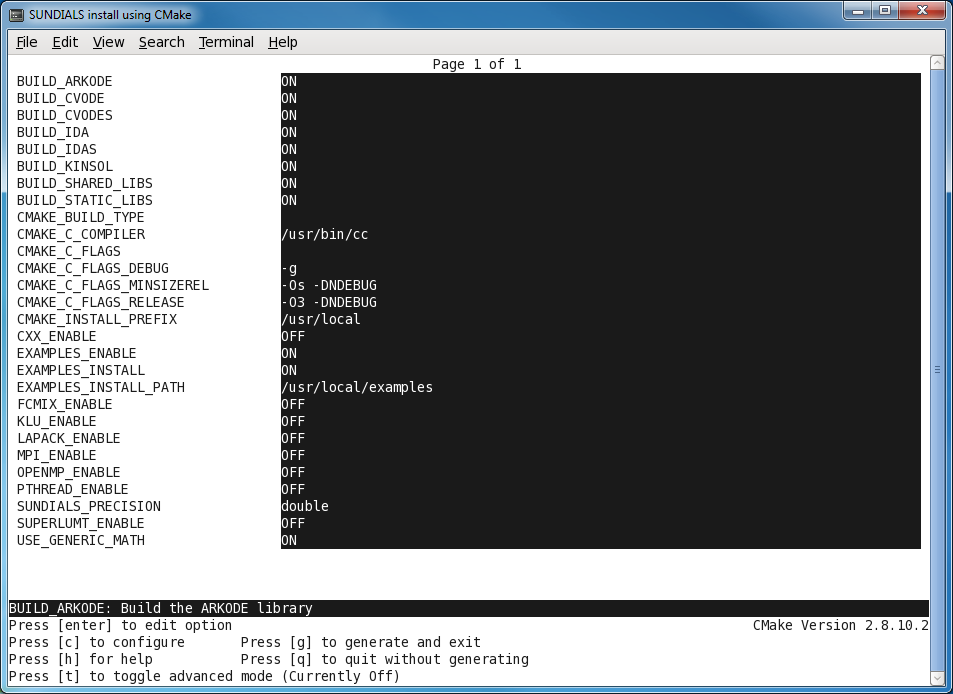
\includegraphics{ccmakedefault.png}}
\caption{Default configuration screen. Note: Initial screen is empty.
To get this default configuration, press `c' repeatedly (accepting
default values denoted with asterisk) until the `g' option is
available.}\label{Install:ccmakedefault}\end{figure}

The default INSTDIR for both SUNDIALS and corresponding examples
can be changed by setting the \code{CMAKE\_INSTALL\_PREFIX} and
the \code{EXAMPLES\_INSTALL\_PATH} as shown in the following figure.
\begin{figure}[htbp]
\centering
\capstart

\scalebox{0.750000}{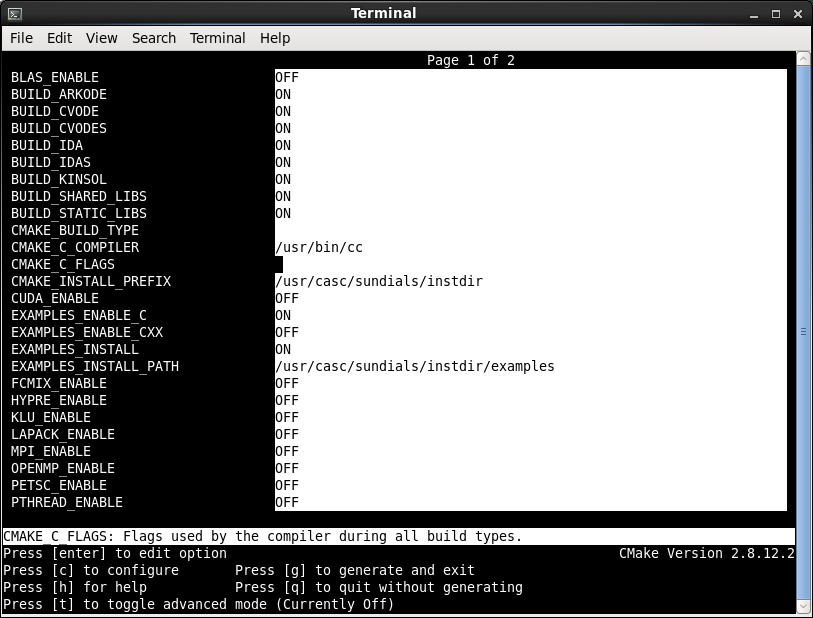
\includegraphics{ccmakeprefix.png}}
\caption{Changing the INSTDIR for SUNDIALS and corresponding EXAMPLES.}\label{Install:ccmakeprefix}\end{figure}

Pressing the \code{g} key or clicking \code{generate} will generate
makefiles including all dependencies and all rules to build SUNDIALS
on this system.  Back at the command prompt, you can now run:

\begin{Verbatim}[commandchars=\\\{\}]
\PYGZdl{} make
\end{Verbatim}

or for a faster parallel build (e.g. using 4 threads), you can run

\begin{Verbatim}[commandchars=\\\{\}]
\PYGZdl{} make \PYGZhy{}j \PYG{l+m}{4}
\end{Verbatim}

To install SUNDIALS in the installation directory specified in the configuration, simply run:

\begin{Verbatim}[commandchars=\\\{\}]
\PYGZdl{} make install
\end{Verbatim}

\index{cmake}

\subsubsection{Building from the command line}
\label{Install:building-from-the-command-line}\label{Install:index-3}
Using CMake from the command line is simply a matter of specifying
CMake variable settings with the \code{cmake} command.  The following
will build the default configuration:

\begin{Verbatim}[commandchars=\\\{\}]
\PYGZdl{} cmake \PYGZhy{}DCMAKE\PYGZus{}INSTALL\PYGZus{}PREFIX\PYG{o}{=}/home/myname/sundials/instdir \PYG{l+s+se}{\PYGZbs{}}
\PYGZgt{}  \PYGZhy{}DEXAMPLES\PYGZus{}INSTALL\PYGZus{}PATH\PYG{o}{=}/home/myname/sundials/instdir/examples \PYG{l+s+se}{\PYGZbs{}}
\PYGZgt{}  ../srcdir
\PYGZdl{} make
\PYGZdl{} make install
\end{Verbatim}


\subsection{Configuration options (Unix/Linux)}
\label{Install:installation-cmake-options}\label{Install:configuration-options-unix-linux}
A complete list of all available options for a CMake-based SUNDIALS
configuration is provide below.  Note that the default values shown
are for a typical configuration on a Linux system and are provided as
illustration only.
\begin{description}
\item[{\index{BUILD\_ARKODE (CMake option)}BUILD\_ARKODE}] \leavevmode
Build the ARKODE library

Default: \code{ON}

\item[{\index{BUILD\_CVODE (CMake option)}BUILD\_CVODE}] \leavevmode
Build the CVODE library

Default: \code{ON}

\item[{\index{BUILD\_CVODES (CMake option)}BUILD\_CVODES}] \leavevmode
Build the CVODES library

Default: \code{ON}

\item[{\index{BUILD\_IDA (CMake option)}BUILD\_IDA}] \leavevmode
Build the IDA library

Default: \code{ON}

\item[{\index{BUILD\_IDAS (CMake option)}BUILD\_IDAS}] \leavevmode
Build the IDAS library

Default: \code{ON}

\item[{\index{BUILD\_KINSOL (CMake option)}BUILD\_KINSOL}] \leavevmode
Build the KINSOL library

Default: \code{ON}

\item[{\index{BUILD\_SHARED\_LIBS (CMake option)}BUILD\_SHARED\_LIBS}] \leavevmode
Build shared libraries

Default: \code{ON}

\item[{\index{BUILD\_STATIC\_LIBS (CMake option)}BUILD\_STATIC\_LIBS}] \leavevmode
Build static libraries

Default: \code{ON}

\item[{\index{CMAKE\_BUILD\_TYPE (CMake option)}CMAKE\_BUILD\_TYPE}] \leavevmode
Choose the type of build, options are:
\code{None} (\code{CMAKE\_C\_FLAGS} used), \code{Debug}, \code{Release},
\code{RelWithDebInfo}, and \code{MinSizeRel}

Default:

\begin{notice}{note}{Note:}
Specifying a build type will trigger the corresponding
build type specific compiler flag options below which
will be appended to the flags set by
\code{CMAKE\_\textless{}language\textgreater{}\_FLAGS}.
\end{notice}

\item[{\index{CMAKE\_C\_COMPILER (CMake option)}CMAKE\_C\_COMPILER}] \leavevmode
C compiler

Default: \code{/usr/bin/cc}

\item[{\index{CMAKE\_C\_FLAGS (CMake option)}CMAKE\_C\_FLAGS}] \leavevmode
Flags for C compiler

Default:

\item[{\index{CMAKE\_C\_FLAGS\_DEBUG (CMake option)}CMAKE\_C\_FLAGS\_DEBUG}] \leavevmode
Flags used by the C compiler during debug
builds

Default: \code{-g}

\item[{\index{CMAKE\_C\_FLAGS\_MINSIZEREL (CMake option)}CMAKE\_C\_FLAGS\_MINSIZEREL}] \leavevmode
Flags used by the C compiler during release minsize builds

Default: \code{-Os -DNDEBUG}

\item[{\index{CMAKE\_C\_FLAGS\_RELEASE (CMake option)}CMAKE\_C\_FLAGS\_RELEASE}] \leavevmode
Flags used by the C compiler during release
builds

Default: \code{-O3 -DNDEBUG}

\item[{\index{CMAKE\_CXX\_COMPILER (CMake option)}CMAKE\_CXX\_COMPILER}] \leavevmode
C++ compiler

Default: \code{/usr/bin/c++}

\begin{notice}{note}{Note:}
A C++ compiler (and all related options) are only are
triggered if C++ examples are enabled
(\code{EXAMPLES\_ENABLE\_CXX} is ON). All SUNDIALS solvers can
be used from C++ applications by default without setting
any additional configuration options.
\end{notice}

\item[{\index{CMAKE\_CXX\_FLAGS (CMake option)}CMAKE\_CXX\_FLAGS}] \leavevmode
Flags for C++ compiler

Default:

\item[{\index{CMAKE\_CXX\_FLAGS\_DEBUG (CMake option)}CMAKE\_CXX\_FLAGS\_DEBUG}] \leavevmode
Flags used by the C++ compiler during debug builds

Default: \code{-g}

\item[{\index{CMAKE\_CXX\_FLAGS\_MINSIZEREL (CMake option)}CMAKE\_CXX\_FLAGS\_MINSIZEREL}] \leavevmode
Flags used by the C++ compiler during release minsize builds

Default: \code{-Os -DNDEBUG}

\item[{\index{CMAKE\_CXX\_FLAGS\_RELEASE (CMake option)}CMAKE\_CXX\_FLAGS\_RELEASE}] \leavevmode
Flags used by the C++ compiler during release builds

Default: \code{-O3 -DNDEBUG}

\item[{\index{CMAKE\_Fortran\_COMPILER (CMake option)}CMAKE\_Fortran\_COMPILER}] \leavevmode
Fortran compiler

Default: \code{/usr/bin/gfortran}

\begin{notice}{note}{Note:}
Fortran support (and all related options) are triggered only if
either Fortran-C support is (\code{FCMIX\_ENABLE} is ON) or
LAPACK support is enabled (\code{LAPACK\_ENABLE} is \code{ON}).
\end{notice}

\item[{\index{CMAKE\_Fortran\_FLAGS (CMake option)}CMAKE\_Fortran\_FLAGS}] \leavevmode
Flags for Fortran compiler

Default:

\item[{\index{CMAKE\_Fortran\_FLAGS\_DEBUG (CMake option)}CMAKE\_Fortran\_FLAGS\_DEBUG}] \leavevmode
Flags used by the Fortran compiler during debug builds

Default: \code{-g}

\item[{\index{CMAKE\_Fortran\_FLAGS\_MINSIZEREL (CMake option)}CMAKE\_Fortran\_FLAGS\_MINSIZEREL}] \leavevmode
Flags used by the Fortran compiler during release minsize builds

Default: \code{-Os}

\item[{\index{CMAKE\_Fortran\_FLAGS\_RELEASE (CMake option)}CMAKE\_Fortran\_FLAGS\_RELEASE}] \leavevmode
Flags used by the Fortran compiler during release builds

Default: \code{-O3}

\item[{\index{CMAKE\_INSTALL\_PREFIX (CMake option)}CMAKE\_INSTALL\_PREFIX}] \leavevmode
Install path prefix, prepended onto install directories

Default: \code{/usr/local}

\begin{notice}{note}{Note:}
The user must have write access to the location specified
through this option. Exported SUNDIALS header files and libraries
will be installed under subdirectories \code{include} and \code{lib} of
\code{CMAKE\_INSTALL\_PREFIX}, respectively.
\end{notice}

\item[{\index{CXX\_ENABLE (CMake option)}CXX\_ENABLE}] \leavevmode
Flag to enable C++ ARKode examples (if examples are enabled)

Default: \code{OFF}

\item[{\index{CUDA\_ENABLE (CMake option)}CUDA\_ENABLE}] \leavevmode
Build the SUNDIALS CUDA vector module.

Default: \code{OFF}

\item[{\index{EXAMPLES\_ENABLE\_C (CMake option)}EXAMPLES\_ENABLE\_C}] \leavevmode
Build the SUNDIALS C examples

Default: \code{ON}

\item[{\index{EXAMPLES\_ENABLE\_CUDA (CMake option)}EXAMPLES\_ENABLE\_CUDA}] \leavevmode
Build the SUNDIALS CUDA examples

Default: \code{OFF}

\begin{notice}{note}{Note:}
You need to enable CUDA support to build these examples.
\end{notice}

\item[{\index{EXAMPLES\_ENABLE\_CXX (CMake option)}EXAMPLES\_ENABLE\_CXX}] \leavevmode
Build the SUNDIALS C++ examples

Default: \code{OFF}

\item[{\index{EXAMPLES\_ENABLE\_F77 (CMake option)}EXAMPLES\_ENABLE\_F77}] \leavevmode
Build the SUNDIALS Fortran77 examples

Default: \code{ON} (if \code{FCMIX\_ENABLE} is \code{ON})

\item[{\index{EXAMPLES\_ENABLE\_F90 (CMake option)}EXAMPLES\_ENABLE\_F90}] \leavevmode
Build the SUNDIALS Fortran90 examples

Default: \code{ON} (if \code{F77\_INTERFACE\_ENABLE} is \code{ON})

\item[{\index{EXAMPLES\_ENABLE\_F2003 (CMake option)}EXAMPLES\_ENABLE\_F2003}] \leavevmode
Build the SUNDIALS Fortran2003 examples

Default: \code{ON} (if \code{F2003\_INTERFACE\_ENABLE} is \code{ON})

\item[{\index{EXAMPLES\_INSTALL (CMake option)}EXAMPLES\_INSTALL}] \leavevmode
Install example files

Default: \code{ON}

\begin{notice}{note}{Note:}
This option is triggered when any of the SUNDIALS
example programs are enabled
(\code{EXAMPLES\_ENABLE\_\textless{}language\textgreater{}} is \code{ON}). If the user
requires installation of example programs then the
sources and sample output files for all SUNDIALS modules
that are currently enabled will be exported to the
directory specified by \code{EXAMPLES\_INSTALL\_PATH}. A CMake
configuration script will also be automatically generated
and exported to the same directory. Additionally, if the
configuration is done under a Unix-like system, makefiles
for the compilation of the example programs (using the
installed SUNDIALS libraries) will be automatically
generated and exported to the directory specified by
\code{EXAMPLES\_INSTALL\_PATH}.
\end{notice}

\item[{\index{EXAMPLES\_INSTALL\_PATH (CMake option)}EXAMPLES\_INSTALL\_PATH}] \leavevmode
Output directory for installing example
files

Default: \code{/usr/local/examples}

\begin{notice}{note}{Note:}
The actual default value for this option will be an
\code{examples} subdirectory created under \code{CMAKE\_INSTALL\_PREFIX}.
\end{notice}

\item[{\index{F77\_INTERFACE\_ENABLE (CMake option)}F77\_INTERFACE\_ENABLE}] \leavevmode
Enable Fortran77-C interface

Default: \code{OFF}

\item[{\index{F2003\_INTERFACE\_ENABLE (CMake option)}F2003\_INTERFACE\_ENABLE}] \leavevmode
Enable Fortran2003 interface

Default: \code{OFF}

\item[{\index{HYPRE\_ENABLE (CMake option)}HYPRE\_ENABLE}] \leavevmode
Flag to enable \emph{hypre} support

Default: \code{OFF}

\begin{notice}{note}{Note:}
See additional information on building with \emph{hypre}
enabled in  {\hyperref[Install:installation-cmake-externallibraries]{\emph{\DUspan{}{Working with external Libraries}}}}.
\end{notice}

\item[{\index{HYPRE\_INCLUDE\_DIR (CMake option)}HYPRE\_INCLUDE\_DIR}] \leavevmode
Path to \emph{hypre} header files

Default: none

\item[{\index{HYPRE\_LIBRARY (CMake option)}HYPRE\_LIBRARY}] \leavevmode
Path to \emph{hypre} installed library files

Default: none

\item[{\index{F90\_ENABLE (CMake option)}KLU\_ENABLE}] \leavevmode
Enable KLU support

Default: \code{OFF}

\begin{notice}{note}{Note:}
See additional information on building with KLU
enabled in {\hyperref[Install:installation-cmake-externallibraries]{\emph{\DUspan{}{Working with external Libraries}}}}.
\end{notice}

\item[{\index{KLU\_INCLUDE\_DIR (CMake option)}KLU\_INCLUDE\_DIR}] \leavevmode
Path to SuiteSparse header files

Default: none

\item[{\index{KLU\_LIBRARY\_DIR (CMake option)}KLU\_LIBRARY\_DIR}] \leavevmode
Path to SuiteSparse installed library files

Default: none

\item[{\index{LAPACK\_ENABLE (CMake option)}LAPACK\_ENABLE}] \leavevmode
Enable LAPACK support

Default: \code{OFF}

\begin{notice}{note}{Note:}
Setting this option to \code{ON} will trigger additional CMake
options. See additional information on building with
LAPACK enabled in {\hyperref[Install:installation-cmake-externallibraries]{\emph{\DUspan{}{Working with external Libraries}}}}.
\end{notice}

\item[{\index{LAPACK\_LIBRARIES (CMake option)}LAPACK\_LIBRARIES}] \leavevmode
LAPACK (and BLAS) libraries

Default: \code{/usr/lib/liblapack.so;/usr/lib/libblas.so}

\begin{notice}{note}{Note:}
CMake will search for libraries in your
\code{LD\_LIBRARY\_PATH} prior to searching default system
paths.
\end{notice}

\item[{\index{MPI\_ENABLE (CMake option)}MPI\_ENABLE}] \leavevmode
Enable MPI support. This will build the parallel nvector
and the MPI-aware version of the ManyVector library.

Default: \code{OFF}

\begin{notice}{note}{Note:}
Setting this option to \code{ON} will trigger several additional
options related to MPI.
\end{notice}

\item[{\index{MPI\_C\_COMPILER (CMake option)}MPI\_C\_COMPILER}] \leavevmode
\code{mpicc} program

Default:

\item[{\index{MPI\_CXX\_COMPILER (CMake option)}MPI\_CXX\_COMPILER}] \leavevmode
\code{mpicxx} program

Default:

\begin{notice}{note}{Note:}
This option is triggered only if MPI is enabled
(\code{MPI\_ENABLE} is \code{ON}) and C++ examples are enabled
(\code{EXAMPLES\_ENABLE\_CXX} is \code{ON}). All SUNDIALS
solvers can be used from C++ MPI applications by default
without setting any additional configuration options
other than \code{MPI\_ENABLE}.
\end{notice}

\item[{\index{MPI\_Fortran\_COMPILER (CMake option)}MPI\_Fortran\_COMPILER}] \leavevmode
\code{mpif77} or \code{mpif90} program

Default:

\begin{notice}{note}{Note:}
This option is triggered only if MPI is enabled
(\code{MPI\_ENABLE} is \code{ON}) and Fortran-C support is
enabled (\code{EXAMPLES\_ENABLE\_F77} or \code{EXAMPLES\_ENABLE\_F90} are \code{ON}).
\end{notice}

\item[{\index{MPIEXEC\_EXECUTABLE (CMake option)}MPIEXEC\_EXECUTABLE}] \leavevmode
Specify the executable for running MPI programs

Default: \code{mpirun}

\begin{notice}{note}{Note:}
This option is triggered only if MPI is enabled (\code{MPI\_ENABLE} is \code{ON}).
\end{notice}

\item[{\index{OPENMP\_ENABLE (CMake option)}OPENMP\_ENABLE}] \leavevmode
Enable OpenMP support (build the OpenMP NVector)

Default: \code{OFF}

\item[{\index{PETSC\_ENABLE (CMake option)}PETSC\_ENABLE}] \leavevmode
Enable PETSc support

Default: \code{OFF}

\begin{notice}{note}{Note:}
See additional information on building with
PETSc enabled in {\hyperref[Install:installation-cmake-externallibraries]{\emph{\DUspan{}{Working with external Libraries}}}}.
\end{notice}

\item[{\index{PETSC\_DIR (CMake option)}PETSC\_DIR}] \leavevmode
Path to PETSc installation

Default: none

\item[{\index{PETSC\_LIBRARIES (CMake option)}PETSC\_LIBRARIES (advanced option)}] \leavevmode
Semi-colon separated list of PETSc link libraries. Unless provided by the
user, this is autopopulated based on the PETSc installation found in
\code{PETSC\_DIR}.

Default: none

\item[{\index{PETSC\_INCLUDES (CMake option)}PETSC\_INCLUDES (advanced option)}] \leavevmode
Semi-colon separated list of PETSc include directroies. Unless provided by
the user, this is autopopulated based on the PETSc installation found in
\code{PETSC\_DIR}.

Default: none

\item[{\index{PTHREAD\_ENABLE (CMake option)}PTHREAD\_ENABLE}] \leavevmode
Enable Pthreads support (build the Pthreads NVector)

Default: \code{OFF}

\item[{\index{RAJA\_ENABLE (CMake option)}RAJA\_ENABLE}] \leavevmode
Enable RAJA support (build the RAJA NVector).

Default: OFF

\begin{notice}{note}{Note:}
You need to enable CUDA in order to build the RAJA vector
module.
\end{notice}

\item[{\index{SUNDIALS\_F77\_FUNC\_CASE (CMake option)}SUNDIALS\_F77\_FUNC\_CASE}] \leavevmode
Specify the case to use in the Fortran name-mangling scheme,
options are: \code{lower} or \code{upper}

Default:

Note: The build system will attempt to infer the Fortran
name-mangling scheme using the Fortran compiler. This option should
only be used if a Fortran compiler is not available or to override
the inferred or default (\code{lower}) scheme if one can not be
determined. If used, \code{SUNDIALS\_F77\_FUNC\_UNDERSCORES} must also
be set.

\end{description}
\begin{quote}\begin{description}
\item[{index}] \leavevmode
\emph{SUNDIALS\_F77\_FUNC\_UNDERSCORES \textless{}SUNDIALS\_F77\_FUNC\_UNDERSCORES (CMake option)\textgreater{}}
Specify the number of underscores to append in the Fortran
name-mangling scheme, options are: \code{none}, \code{one}, or \code{two}

Default:

Note: The build system will attempt to infer the Fortran
name-mangling scheme using the Fortran compiler. This option should
only be used if a Fortran compiler is not available or to override
the inferred or default (\code{one}) scheme if one can not be
determined. If used, \code{SUNDIALS\_F77\_FUNC\_CASE} must also be set.

\end{description}\end{quote}
\begin{description}
\item[{\index{SUNDIALS\_INDEX\_TYPE (CMake option)}SUNDIALS\_INDEX\_TYPE (advanced)}] \leavevmode
Integer type used for SUNDIALS indices.  The size must match the size provided for
the \code{SUNDIALS\_INDEX\_SIZE} option.

Default:

Note: In past SUNDIALS versions, a user could set this option to
\code{INT64\_T} to use 64-bit integers, or \code{INT32\_T} to use 32-bit
integers. Starting in SUNDIALS 3.2.0, these special values are
deprecated. For SUNDIALS 3.2.0 and up, a user will only need to use
the \code{SUNDIALS\_INDEX\_SIZE} option in most cases.

\item[{\index{SUNDIALS\_INDEX\_SIZE (CMake option)}SUNDIALS\_INDEX\_SIZE}] \leavevmode
Integer size (in bits) used for indices in SUNDIALS, options are: \code{32} or \code{64}

Default: \code{64}

Note: The build system tries to find an integer type of appropriate
size. Candidate 64-bit integer types are (in order of preference):
\code{int64\_t}, \code{\_\_int64}, \code{long long}, and \code{long}.  Candidate
32-bit integers are (in order of preference): \code{int32\_t},
\code{int}, and \code{long}.  The advanced option,
\code{SUNDIALS\_INDEX\_TYPE} can be used to provide a type not listed
here.

\item[{\index{SUNDIALS\_PRECISION (CMake option)}SUNDIALS\_PRECISION}] \leavevmode
Precision used in SUNDIALS, options are: \code{double}, \code{single} or
\code{extended}

Default: \code{double}

\item[{\index{SUPERLUDIST\_ENABLE (CMake option)}SUPERLUDIST\_ENABLE}] \leavevmode
Enable SuperLU\_DIST support

Default: \code{OFF}

\begin{notice}{note}{Note:}
See additional information on building wtih
SuperLU\_DIST enabled in {\hyperref[Install:installation-cmake-externallibraries]{\emph{\DUspan{}{Working with external Libraries}}}}.
\end{notice}

\item[{\index{SUPERLUDIST\_INCLUDE\_DIR (CMake option)}SUPERLUDIST\_INCLUDE\_DIR}] \leavevmode
Path to SuperLU\_DIST header files (under a typical SuperLU\_DIST
install, this is typically the SuperLU\_DIST \code{SRC} directory)

Default: none

\item[{\index{SUPERLUDIST\_LIBRARY\_DIR (CMake option)}SUPERLUDIST\_LIBRARY\_DIR}] \leavevmode
Path to SuperLU\_DIST installed library files

Default: none

\item[{\index{SUPERLUDIST\_LIBRARIES (CMake option)}SUPERLUDIST\_LIBRARIES}] \leavevmode
Semi-colon separated list of libraries needed for SuperLU\_DIST

Default: none

\item[{\index{SUPERLUDIST\_OpenMP (CMake option)}SUPERLUDIST\_OpenMP}] \leavevmode
Enable SUNDIALS support for SuperLU\_DIST built with OpenMP

Default: none

Note: SuperLU\_DIST must be built with OpenMP support for this option to function.
Additionally the environment variable \code{OMP\_NUM\_THREADS} must be set to the desired
number of threads.

\item[{\index{SUPERLUMT\_ENABLE (CMake option)}SUPERLUMT\_ENABLE}] \leavevmode
Enable SuperLU\_MT support

Default: \code{OFF}

\begin{notice}{note}{Note:}
See additional information on building with
SuperLU\_MT enabled in {\hyperref[Install:installation-cmake-externallibraries]{\emph{\DUspan{}{Working with external Libraries}}}}.
\end{notice}

\item[{\index{SUPERLUMT\_INCLUDE\_DIR (CMake option)}SUPERLUMT\_INCLUDE\_DIR}] \leavevmode
Path to SuperLU\_MT header files (under a typical SuperLU\_MT
install, this is typically the SuperLU\_MT \code{SRC} directory)

Default: none

\item[{\index{SUPERLUMT\_LIBRARY\_DIR (CMake option)}SUPERLUMT\_LIBRARY\_DIR}] \leavevmode
Path to SuperLU\_MT installed library files

Default: none

\item[{\index{SUPERLUMT\_THREAD\_TYPE (CMake option)}SUPERLUMT\_THREAD\_TYPE}] \leavevmode
Must be set to Pthread or OpenMP, depending on how SuperLU\_MT was compiled.

Default: Pthread

\item[{\index{USE\_GENERIC\_MATH (CMake option)}USE\_GENERIC\_MATH}] \leavevmode
Use generic (\code{stdc}) math libraries

Default: \code{ON}

\end{description}


\subsubsection{xSDK Configuration Options}
\label{Install:installation-cmake-xsdk}\label{Install:xsdk-configuration-options}
SUNDIALS supports CMake configuration options defined by the
Extreme-scale Scientific Software Development Kit (xSDK) community
policies (see \href{https://xsdk.info}{https://xsdk.info} for more
information). xSDK CMake options are unused by default but may be
activated by setting \code{USE\_XSDK\_DEFAULTS} to \code{ON}.

\begin{notice}{note}{Note:}
When xSDK options are active, they will overwrite the
corresponding SUNDIALS option and may have different
default values (see details below). As such the equivalent
SUNDIALS options should not be used when configuring with
xSDK options. In the GUI front end to CMake (\code{ccmake} or
\code{cmake-gui}), setting \code{USE\_XSDK\_DEFAULTS} to ON will
hide the corresponding SUNDIALS options as advanced CMake
variables. During configuration, messages are output
detailing which xSDK flags are active and the equivalent
SUNDIALS options that are replaced. Below is a complete list
xSDK options and the corresponding SUNDIALS options if
applicable.
\end{notice}
\begin{description}
\item[{\index{TPL\_ENABLE\_HYPRE (xSDK CMake option)}TPL\_ENABLE\_HYPRE}] \leavevmode
Enable \emph{hypre} support

Default: \code{OFF}

SUNDIALS equivalent: \code{HYPRE\_ENABLE}

\item[{\index{TPL\_ENABLE\_KLU (xSDK CMake option)}TPL\_ENABLE\_KLU}] \leavevmode
Enable KLU support

Default: \code{OFF}

SUNDIALS equivalent: \code{KLU\_ENABLE}

\item[{\index{TPL\_ENABLE\_PETSC (xSDK CMake option)}TPL\_ENABLE\_PETSC}] \leavevmode
Enable PETSc support

Default: \code{OFF}

SUNDIALS equivalent: \code{PETSC\_ENABLE}

\item[{\index{TPL\_ENABLE\_LAPACK (xSDK CMake option)}TPL\_ENABLE\_LAPACK}] \leavevmode
Enable LAPACK support

Default: \code{OFF}

SUNDIALS equivalent: \code{LAPACK\_ENABLE}

\item[{\index{TPL\_ENABLE\_SUPERLUDIST (xSDK CMake option)}TPL\_ENABLE\_SUPERLUDIST}] \leavevmode
Enable SuperLU\_DIST support

Default: \code{OFF}

SUNDIALS equivalent: \code{SUPERLUDIST\_ENABLE}

\item[{\index{TPL\_ENABLE\_SUPERLUMT (xSDK CMake option)}TPL\_ENABLE\_SUPERLUMT}] \leavevmode
Enable SuperLU\_MT support

Default: \code{OFF}

SUNDIALS equivalent: \code{SUPERLUMT\_ENABLE}

\item[{\index{TPL\_HYPRE\_INCLUDE\_DIRS (xSDK CMake option)}TPL\_HYPRE\_INCLUDE\_DIRS}] \leavevmode
Path to \emph{hypre} header files

SUNDIALS equivalent: \code{HYPRE\_INCLUDE\_DIR}

\item[{\index{TPL\_HYPRE\_LIBRARIES (xSDK CMake option)}TPL\_HYPRE\_LIBRARIES}] \leavevmode
\emph{hypre} library

SUNDIALS equivalent: N/A

\item[{\index{TPL\_KLU\_INCLUDE\_DIRS (xSDK CMake option)}TPL\_KLU\_INCLUDE\_DIRS}] \leavevmode
Path to KLU header files

SUNDIALS equivalent: \code{KLU\_INCLUDE\_DIR}

\item[{\index{TPL\_KLU\_LIBRARIES (xSDK CMake option)}TPL\_KLU\_LIBRARIES}] \leavevmode
KLU library

SUNDIALS equivalent: N/A

\item[{\index{TPL\_LAPACK\_LIBRARIES (xSDK CMake option)}TPL\_LAPACK\_LIBRARIES}] \leavevmode
LAPACK (and BLAS) libraries

Default: \code{/usr/lib/liblapack.so;/usr/lib/libblas.so}

SUNDIALS equivalent: \code{LAPACK\_LIBRARIES}

\begin{notice}{note}{Note:}
CMake will search for libraries in your
\code{LD\_LIBRARY\_PATH} prior to searching default system paths.
\end{notice}

\item[{\index{TPL\_PETSC\_DIR (xSDK CMake option)}TPL\_PETSC\_DIR}] \leavevmode
Path to PETSc installtion

SUNDIALS equivalent: \code{PETSC\_DIR}

\item[{\index{TPL\_SUPERLUDIST\_INCLUDE\_DIRS (xSDK CMake option)}TPL\_SUPERLUDIST\_INCLUDE\_DIRS}] \leavevmode
Path to SuperLU\_DIST header files

SUNDIALS equivalent: \code{SUPERLUDIST\_INCLUDE\_DIR}

\item[{\index{TPL\_SUPERLUDIST\_LIBRARIES (xSDK CMake option)}TPL\_SUPERLUDIST\_LIBRARIES}] \leavevmode
Semi-colon separated list of libraries needed for SuperLU\_DIST including
the SuperLU\_DIST library itself

SUNDIALS equivalent: \code{SUPERLUDIST\_LIBRARIES}

\item[{\index{TPL\_SUPERLUDIST\_OpenMP (xSDK CMake option)}TPL\_SUPERLUDIST\_OpenMP}] \leavevmode
Enable SUNDIALS support for SuperLU\_DIST built with OpenMP

SUNDIALS equivalent: \code{SUPERLUDIST\_OpenMP}

\item[{\index{TPL\_SUPERLUMT\_INCLUDE\_DIRS (xSDK CMake option)}TPL\_SUPERLUMT\_INCLUDE\_DIRS}] \leavevmode
Path to SuperLU\_MT header files

SUNDIALS equivalent: \code{SUPERLUMT\_INCLUDE\_DIR}

\item[{\index{TPL\_SUPERLUMT\_LIBRARIES (xSDK CMake option)}TPL\_SUPERLUMT\_LIBRARIES}] \leavevmode
SuperLU\_MT library

SUNDIALS equivalent: N/A

\item[{\index{TPL\_SUPERLUMT\_THREAD\_TYPE (xSDK CMake option)}TPL\_SUPERLUMT\_THREAD\_TYPE}] \leavevmode
SuperLU\_MT library thread type

SUNDIALS equivalent: \code{SUPERLUMT\_THREAD\_TYPE}

\item[{\index{USE\_XSDK\_DEFAULTS (xSDK CMake option)}USE\_XSDK\_DEFAULTS}] \leavevmode
Enable xSDK default configuration settings

Default: \code{OFF}

SUNDIALS equivalent: N/A

\begin{notice}{note}{Note:}
Enabling xSDK defaults also sets \code{CMAKE\_BUILD\_TYPE} to \code{Debug}
\end{notice}

\item[{\index{XSDK\_ENABLE\_FORTRAN (xSDK CMake option)}XSDK\_ENABLE\_FORTRAN}] \leavevmode
Enable SUNDIALS Fortran interface

Default: \code{OFF}

SUNDIALS equivalent: \code{FCMIX\_ENABLE}

\item[{\index{XSDK\_INDEX\_SIZE (xSDK CMake option)}XSDK\_INDEX\_SIZE}] \leavevmode
Integer size (bits) used for indices in SUNDIALS, options are: \code{32} or \code{64}

Default: \code{32}

SUNDIALS equivalent: \code{SUNDIALS\_INDEX\_SIZE}

\item[{\index{XSDK\_PRECISION (xSDK CMake option)}XSDK\_PRECISION}] \leavevmode
Precision used in SUNDIALS, options are: \code{double}, \code{single}, or \code{quad}

Default: \code{double}

SUNDIALS equivalent: \code{SUNDIALS\_PRECISION}

\end{description}


\subsection{Configuration examples}
\label{Install:configuration-examples}\label{Install:installation-cmake-examples}
The following examples will help demonstrate usage of the CMake
configure options.

To configure SUNDIALS using the default C and Fortran compilers,
and default \code{mpicc} and \code{mpif77} parallel compilers,
enable compilation of examples, and install libraries, headers, and
example sources under subdirectories of \code{/home/myname/sundials/}, use:

\begin{Verbatim}[commandchars=\\\{\}]
\PYGZpc{} cmake \PYG{l+s+se}{\PYGZbs{}}
\PYGZgt{} \PYGZhy{}DCMAKE\PYGZus{}INSTALL\PYGZus{}PREFIX\PYG{o}{=}/home/myname/sundials/instdir \PYG{l+s+se}{\PYGZbs{}}
\PYGZgt{} \PYGZhy{}DEXAMPLES\PYGZus{}INSTALL\PYGZus{}PATH\PYG{o}{=}/home/myname/sundials/instdir/examples \PYG{l+s+se}{\PYGZbs{}}
\PYGZgt{} \PYGZhy{}DMPI\PYGZus{}ENABLE\PYG{o}{=}ON \PYG{l+s+se}{\PYGZbs{}}
\PYGZgt{} \PYGZhy{}DFCMIX\PYGZus{}ENABLE\PYG{o}{=}ON \PYG{l+s+se}{\PYGZbs{}}
\PYGZgt{} /home/myname/sundials/srcdir

\PYGZpc{} make install
\end{Verbatim}

To disable installation of the examples, use:

\begin{Verbatim}[commandchars=\\\{\}]
\PYGZpc{} cmake \PYG{l+s+se}{\PYGZbs{}}
\PYGZgt{} \PYGZhy{}DCMAKE\PYGZus{}INSTALL\PYGZus{}PREFIX\PYG{o}{=}/home/myname/sundials/instdir \PYG{l+s+se}{\PYGZbs{}}
\PYGZgt{} \PYGZhy{}DEXAMPLES\PYGZus{}INSTALL\PYGZus{}PATH\PYG{o}{=}/home/myname/sundials/instdir/examples \PYG{l+s+se}{\PYGZbs{}}
\PYGZgt{} \PYGZhy{}DMPI\PYGZus{}ENABLE\PYG{o}{=}ON \PYG{l+s+se}{\PYGZbs{}}
\PYGZgt{} \PYGZhy{}DFCMIX\PYGZus{}ENABLE\PYG{o}{=}ON \PYG{l+s+se}{\PYGZbs{}}
\PYGZgt{} \PYGZhy{}DEXAMPLES\PYGZus{}INSTALL\PYG{o}{=}OFF \PYG{l+s+se}{\PYGZbs{}}
\PYGZgt{} /home/myname/sundials/srcdir

\PYGZpc{} make install
\end{Verbatim}


\subsection{Working with external Libraries}
\label{Install:installation-cmake-externallibraries}\label{Install:working-with-external-libraries}
The SUNDIALS suite contains many options to enable implementation
flexibility when developing solutions. The following are some notes
addressing specific configurations when using the supported third
party libraries.


\subsubsection{Building with LAPACK}
\label{Install:building-with-lapack}\label{Install:installation-cmake-externallibraries-lapack}
To enable LAPACK, set the \code{LAPACK\_ENABLE} option to \code{ON}.
If the directory containing the LAPACK library is in the
\code{LD\_LIBRARY\_PATH} environment variable, CMake will set the
\code{LAPACK\_LIBRARIES} variable accordingly, otherwise CMake will
attempt to find the LAPACK library in standard system locations. To
explicitly tell CMake what library to use, the \code{LAPACK\_LIBRARIES}
variable can be set to the desired libraries required for LAPACK.

\begin{Verbatim}[commandchars=\\\{\}]
\PYGZpc{} cmake \PYG{l+s+se}{\PYGZbs{}}
\PYGZgt{} \PYGZhy{}DCMAKE\PYGZus{}INSTALL\PYGZus{}PREFIX\PYG{o}{=}/home/myname/sundials/instdir \PYG{l+s+se}{\PYGZbs{}}
\PYGZgt{} \PYGZhy{}DEXAMPLES\PYGZus{}INSTALL\PYGZus{}PATH\PYG{o}{=}/home/myname/sundials/instdir/examples \PYG{l+s+se}{\PYGZbs{}}
\PYGZgt{} \PYGZhy{}DLAPACK\PYGZus{}ENABLE\PYG{o}{=}ON \PYG{l+s+se}{\PYGZbs{}}
\PYGZgt{} \PYGZhy{}DLAPACK\PYGZus{}LIBRARIES\PYG{o}{=}/mylapackpath/lib/libblas.so\PYG{p}{;}/mylapackpath/lib/liblapack.so \PYG{l+s+se}{\PYGZbs{}}
\PYGZgt{} /home/myname/sundials/srcdir

\PYGZpc{} make install
\end{Verbatim}

\begin{notice}{note}{Note:}
If a working Fortran compiler is not available to infer the
Fortran name-mangling scheme, the options
\code{SUNDIALS\_F77\_FUNC\_CASE} and
\code{SUNDIALS\_F77\_FUNC\_UNDERSCORES} \emph{must} be set in order to
bypass the check for a Fortran compiler and define the
name-mangling scheme. The defaults for these options in
earlier versions of SUNDIALS were \code{lower} and \code{one},
respectively.
\end{notice}


\subsubsection{Building with KLU}
\label{Install:installation-cmake-externallibraries-klu}\label{Install:building-with-klu}
The KLU libraries are part of SuiteSparse, a suite of sparse matrix
software, available from the Texas A\&M University website:
\href{http://faculty.cse.tamu.edu/davis/suitesparse.html}{http://faculty.cse.tamu.edu/davis/suitesparse.html} .

SUNDIALS has been tested with SuiteSparse version 4.5.3.  To enable
KLU, set \code{KLU\_ENABLE} to \code{ON}, set \code{KLU\_INCLUDE\_DIR} to the
\code{include} path of the KLU installation and set \code{KLU\_LIBRARY\_DIR}
to the \code{lib} path of the KLU installation.  The CMake configure will
result in populating the following variables: \code{AMD\_LIBRARY},
\code{AMD\_LIBRARY\_DIR},  \code{BTF\_LIBRARY}, \code{BTF\_LIBRARY\_DIR},
\code{COLAMD\_LIBRARY}, \code{COLAMD\_LIBRARY\_DIR}, and \code{KLU\_LIBRARY}.


\subsubsection{Building with SuperLU\_DIST}
\label{Install:building-with-superlu-dist}\label{Install:installation-cmake-externallibraries-superlu-mt}
The SuperLU\_DIST libraries are available for download from the Lawrence
Berkeley National Laboratory website:
\href{http://crd-legacy.lbl.gov/\$sim\$xiaoye/SuperLU/}{http://crd-legacy.lbl.gov/\$sim\$xiaoye/SuperLU/}\#superlu\_dist.

SUNDIALS has been tested with SuperLU\_DIST greater than 6.1. To enable
SuperLU\_DIST, set  \code{SUPERLUDIST\_ENABLE} to \code{ON}, set
\code{SUPERLUDIST\_INCLUDE\_DIR} to the \code{SRC} path of the SuperLU\_DIST
installation, and set the variable \code{SUPERLUMT\_LIBRARY\_DIR} to the
\code{lib} path of the SuperLU\_DIST installation.  At the same time, the
variable \code{SUPERLUDIST\_LIBRARIES} must be set to a semi-colon separated list
of other libraries SuperLU\_DIST depends on. For example, if SuperLU\_DIST
was built with LAPACK, then include the LAPACK library in this list.
If SuperLU\_DIST was built with OpenMP support, then you may set
\code{SUPERLUDIST\_OpenMP} to \code{ON} utilize the OpenMP functionality of
SuperLU\_DIST.


\subsubsection{Building with SuperLU\_MT}
\label{Install:building-with-superlu-mt}
The SuperLU\_MT libraries are available for download from the Lawrence
Berkeley National Laboratory website:
\href{http://crd-legacy.lbl.gov/\$sim\$xiaoye/SuperLU/}{http://crd-legacy.lbl.gov/\$sim\$xiaoye/SuperLU/}\#superlu\_mt .

SUNDIALS has been tested with SuperLU\_MT version 3.1.  To enable
SuperLU\_MT, set  \code{SUPERLUMT\_ENABLE} to \code{ON}, set
\code{SUPERLUMT\_INCLUDE\_DIR} to the \code{SRC} path of the SuperLU\_MT
installation, and set the variable \code{SUPERLUMT\_LIBRARY\_DIR} to the
\code{lib} path of the SuperLU\_MT installation. At the same time, the
variable \code{SUPERLUMT\_LIBRARIES} must be set to a semi-colon separated
list of other libraries SuperLU\_MT depends on. For example, if
SuperLU\_MT was build with an external blas library, then include the
full path to the blas library in this list. Additionally, the
variable \code{SUPERLUMT\_THREAD\_TYPE} must be set to either \code{Pthread}
or \code{OpenMP}.

Do not mix thread types when building SUNDIALS solvers.
If threading is enabled for SUNDIALS by having either
\code{OPENMP\_ENABLE} or \code{PTHREAD\_ENABLE} set to \code{ON} then SuperLU\_MT
should be set to use the same threading type.


\subsubsection{Building with PETSc}
\label{Install:building-with-petsc}\label{Install:installation-cmake-externallibraries-petsc}
The PETSc libraries are available for download from the Argonne
National Laboratory website:
\href{http://www.mcs.anl.gov/petsc}{http://www.mcs.anl.gov/petsc} .

SUNDIALS has been tested with PETSc version 3.10.0 - 3.12.0.  To enable
PETSc, set \code{PETSC\_ENABLE} to \code{ON}, and set \code{PETSC\_DIR} to the
path of the PETSc installation.


\subsubsection{Building with \emph{hypre}}
\label{Install:building-with-hypre}\label{Install:installation-cmake-externallibraries-hypre}
The \emph{hypre} libraries are available for download from the Lawrence
Livermore National Laboratory website:
\href{http://computing.llnl.gov/projects/hypre}{http://computing.llnl.gov/projects/hypre}.
SUNDIALS has been tested with \emph{hypre} version 2.11.1.
To enable \emph{hypre}, set  \code{HYPRE\_ENABLE} to \code{ON}, set \code{HYPRE\_INCLUDE\_DIR}
to the \code{include} path of the \emph{hypre} installation, and set the variable
\code{HYPRE\_LIBRARY\_DIR} to the \code{lib} path of the \emph{hypre} installation.

Note: SUNDIALS must be configured so that \code{SUNDIALS\_INDEX\_SIZE} (or
equivalently, \code{XSDK\_INDEX\_SIZE}) equals the precision of
\code{HYPRE\_BigInt} in the corresponding \emph{hypre} installation.


\subsubsection{Building with CUDA}
\label{Install:installation-cmake-externallibraries-cuda}\label{Install:building-with-cuda}
SUNDIALS CUDA modules and examples have been tested with version 8.0 of the
CUDA toolkit. To build them, you need to install the Toolkit and compatible
NVIDIA drivers. Both are available for download from the NVIDIA website:
\href{https://developer.nvidia.com/cuda-downloads}{https://developer.nvidia.com/cuda-downloads}. To enable CUDA,
set \code{CUDA\_ENABLE} to \code{ON}. If CUDA is installed in a nonstandard
location, you may be prompted to set the variable
\code{CUDA\_TOOLKIT\_ROOT\_DIR} with your CUDA Toolkit installation
path. To enable CUDA examples, set \code{EXAMPLES\_ENABLE\_CUDA} to \code{ON}.


\subsubsection{Building with RAJA}
\label{Install:building-with-raja}\label{Install:installation-cmake-externallibraries-raja}
RAJA is a performance portability layer developed by Lawrence
Livermore National Laboratory and can be obtained from \{tt
\href{https://github.com/LLNL/RAJA}{https://github.com/LLNL/RAJA}.
SUNDIALS RAJA modules and examples have been tested with RAJA
version 0.3. Building SUNDIALS RAJA modules requires a CUDA-enabled
RAJA installation. To enable RAJA, set \code{CUDA\_ENABLE} and
\code{RAJA\_ENABLE} to \code{ON}. If RAJA is installed in a nonstandard
location you will be prompted to set the variable \code{RAJA\_DIR} with
the path to the RAJA CMake configuration file. To enable building the
RAJA examples set \code{EXAMPLES\_ENABLE\_CUDA} to \code{ON}.


\subsection{Testing the build and installation}
\label{Install:testing-the-build-and-installation}\label{Install:installation-cmake-testing}
If SUNDIALS was configured with \code{EXAMPLES\_ENABLE\_\textless{}language\textgreater{}} options
to \code{ON}, then a set of regression tests can be run after building
with the \code{make} command by running:

\begin{Verbatim}[commandchars=\\\{\}]
\PYGZpc{} make \PYG{n+nb}{test}
\end{Verbatim}

Additionally, if \code{EXAMPLES\_INSTALL} was also set to \code{ON}, then a
set of smoke tests can be run after installing with the \code{make install}
command by running:

\begin{Verbatim}[commandchars=\\\{\}]
\PYGZpc{} make test\PYGZus{}install
\end{Verbatim}


\subsection{Building and Running Examples}
\label{Install:building-and-running-examples}\label{Install:installation-cmake-buildrunexamples}
Each of the SUNDIALS solvers is distributed with a set of examples
demonstrating basic usage. To build and install the examples, set at
least of the \code{EXAMPLES\_ENABLE\_\textless{}language\textgreater{}} options to \code{ON}, and
set \code{EXAMPLES\_INSTALL} to \code{ON}. Specify
the installation path for the examples with the variable
\code{EXAMPLES\_INSTALL\_PATH}. CMake will generate \code{CMakeLists.txt}
configuration files (and \code{Makefile} files if on Linux/Unix) that
reference the \emph{installed} SUNDIALS headers and libraries.

Either the \code{CMakeLists.txt} file or the traditional \code{Makefile} may
be used to build the examples as well as serve as a template for
creating user developed solutions.  To use the supplied \code{Makefile}
simply run \code{make} to compile and generate the executables.  To use
CMake from within the installed example directory, run \code{cmake} (or
\code{ccmake} or \code{cmake-gui} to use the GUI) followed by \code{make} to
compile the example code.  Note that if CMake is used, it will
overwrite the traditional \code{Makefile} with a new CMake-generated
\code{Makefile}.

The resulting output from running the examples can be compared with
example output bundled in the SUNDIALS distribution.

NOTE: There will potentially be differences in the output due to
machine architecture, compiler versions, use of third party libraries etc.


\subsection{Configuring, building, and installing on Windows}
\label{Install:installation-cmake-windows}\label{Install:configuring-building-and-installing-on-windows}
CMake can also be used to build SUNDIALS on Windows. To build SUNDIALS
for use with Visual Studio the following steps should be performed:
\begin{enumerate}
\item {} 
Unzip the downloaded tar file(s) into a directory. This will be the
\code{SOLVERDIR}

\item {} 
Create a separate \code{BUILDDIR}

\item {} 
Open a Visual Studio Command Prompt and cd to \code{BUILDDIR}

\item {} 
Run \code{cmake-gui ../SOLVERDIR}
\begin{enumerate}
\item {} 
Hit Configure

\item {} 
Check/Uncheck solvers to be built

\item {} 
Change \code{CMAKE\_INSTALL\_PREFIX} to \code{INSTDIR}

\item {} 
Set other options as desired

\item {} 
Hit Generate

\end{enumerate}

\item {} 
Back in the VS Command Window:
\begin{enumerate}
\item {} 
Run \code{msbuild ALL\_BUILD.vcxproj}

\item {} 
Run \code{msbuild INSTALL.vcxproj}

\end{enumerate}

\end{enumerate}

The resulting libraries will be in the \code{INSTDIR}.

The SUNDIALS project can also now be opened in Visual Studio.
Double click on the \code{ALL\_BUILD.vcxproj} file to open the project.
Build the whole \emph{solution} to create the SUNDIALS libraries.
To use the SUNDIALS libraries in your own projects, you must
set the include directories for your project,
add the SUNDIALS libraries to your project solution,
and set the SUNDIALS libraries as dependencies for your project.


\section{Installed libraries and exported header files}
\label{Install:installation-results}\label{Install:installed-libraries-and-exported-header-files}
Using the CMake SUNDIALS build system, the command

\begin{Verbatim}[commandchars=\\\{\}]
\PYGZdl{} make install
\end{Verbatim}

will install the libraries under \code{LIBDIR} and the public header
files under \code{INCLUDEDIR}. The values for these directories
are \code{INSTDIR/lib} and \code{INSTDIR/include}, respectively.  The
location can be changed by setting the CMake variable
\code{CMAKE\_INSTALL\_PREFIX}.  Although all installed libraries reside
under \code{LIBDIR/lib}, the public header files are further organized
into subdirectories under \code{INCLUDEDIR/include}.

The installed libraries and exported header files are listed for
reference in the {\hyperref[Install:installation-table]{\emph{\DUspan{}{Table: SUNDIALS libraries and header files}}}}. The file extension \code{.LIB} is typically \code{.so}
for shared libraries and \code{.a} for static libraries. Note that, in
this table names are relative to \code{LIBDIR} for libraries and to
\code{INCLUDEDIR} for header files.

A typical user program need not explicitly include any of the shared
SUNDIALS header files from under the \code{INCLUDEDIR/include/sundials}
directory since they are explicitly included by the appropriate solver
header files (e.g., \code{cvode\_dense.h} includes
\code{sundials\_dense.h}). However, it is both legal and safe to do so,
and would be useful, for example, if the functions declared in
\code{sundials\_dense.h} are to be used in building a preconditioner.


\subsection{Table: SUNDIALS libraries and header files}
\label{Install:installation-table}\label{Install:table-sundials-libraries-and-header-files}
\begin{longtable}{|l|l|l|}
\hline
\endfirsthead

\multicolumn{3}{c}%
{{\textsf{\tablename\ \thetable{} -- continued from previous page}}} \\
\hline
\endhead

\hline \multicolumn{3}{|r|}{{\textsf{Continued on next page}}} \\ \hline
\endfoot

\endlastfoot


Shared
 & 
Header files
 & 
\code{sundials/sundials\_band.h},
\code{sundials/sundials\_config.h},
\code{sundials/sundials\_dense.h},
\code{sundials/sundials\_direct.h},
\code{sundials/sundials\_fconfig.h},
\code{sundials/sundials\_fnvector.h},
\code{sundials/sundials\_iterative.h},
\code{sundials/sundials\_linearsolver.h},
\code{sundials/sundials\_nonlinearsolver.h},
\code{sundials/sundials\_matrix.h},
\code{sundials/sundials\_math.h},
\code{sundials/sundials\_nvector.h},
\code{sundials/sundials\_types.h},
\code{sundials/sundials\_version.h}
\\
\hline
NVECTOR\_SERIAL
 & 
Libraries
 & 
\code{libsundials\_nvecserial.LIB},
\code{libsundials\_fnvecserial.a}
\\
\hline
NVECTOR\_SERIAL
 & 
Header files
 & 
\code{nvector/nvector\_serial.h}
\\
\hline
NVECTOR\_PARALLEL
 & 
Libraries
 & 
\code{libsundials\_nvecparallel.LIB},
\code{libsundials\_fnvecparallel.a}
\\
\hline
NVECTOR\_PARALLEL
 & 
Header files
 & 
\code{nvector/nvector\_parallel.h}
\\
\hline
NVECTOR\_OPENMP
 & 
Libraries
 & 
\code{libsundials\_nvecopenmp.LIB},
\code{libsundials\_fnvecopenmp.a}
\\
\hline
NVECTOR\_OPENMP
 & 
Header files
 & 
\code{nvector/nvector\_openmp.h}
\\
\hline
NVECTOR\_PTHREADS
 & 
Libraries
 & 
\code{libsundials\_nvecpthreads.LIB},
\code{libsundials\_fnvecpthreads.a}
\\
\hline
NVECTOR\_PTHREADS
 & 
Header files
 & 
\code{nvector/nvector\_pthreads.h}
\\
\hline
NVECTOR\_PARHYP
 & 
Libraries
 & 
\code{libsundials\_nvecparhyp.LIB}
\\
\hline
NVECTOR\_PARHYP
 & 
Header files
 & 
\code{nvector/nvector\_parhyp.h}
\\
\hline
NVECTOR\_PETSC
 & 
Libraries
 & 
\code{libsundials\_nvecpetsc.LIB}
\\
\hline
NVECTOR\_PETSC
 & 
Header files
 & 
\code{nvector/nvector\_petsc.h}
\\
\hline
NVECTOR\_CUDA
 & 
Libraries
 & 
\code{libsundials\_nveccuda.LIB}
\\
\hline
NVECTOR\_CUDA
 & 
Header files
 & 
\code{nvector/nvector\_cuda.h}
\\
\hline
NVECTOR\_RAJA
 & 
Libraries
 & 
\code{libsundials\_nvecraja.LIB}
\\
\hline
NVECTOR\_RAJA
 & 
Header files
 & 
\code{nvector/nvector\_raja.h}
\\
\hline
NVECTOR\_MANYVECTOR
 & 
Libraries
 & 
\code{libsundials\_nvecmanyvector.LIB}
\\
\hline
NVECTOR\_MANYVECTOR
 & 
Header files
 & 
\code{nvector/nvector\_manyvector.h}
\\
\hline
NVECTOR\_MPIMANYVECTOR
 & 
Libraries
 & 
\code{libsundials\_nvecmpimanyvector.LIB}
\\
\hline
NVECTOR\_MPIMANYVECTOR
 & 
Header files
 & 
\code{nvector/nvector\_mpimanyvector.h}
\\
\hline
NVECTOR\_MPIPLUSX
 & 
Libraries
 & 
\code{libsundials\_nvecmpiplusx.LIB}
\\
\hline
NVECTOR\_MPIPLUSX
 & 
Header files
 & 
\code{nvector/nvector\_mpiplusx.h}
\\
\hline
SUNMATRIX\_BAND
 & 
Libraries
 & 
\code{libsundials\_sunmatrixband.LIB},
\code{libsundials\_fsunmatrixband.a}
\\
\hline
SUNMATRIX\_BAND
 & 
Header files
 & 
\code{sunmatrix/sunmatrix\_band.h}
\\
\hline
SUNMATRIX\_DENSE
 & 
Libraries
 & 
\code{libsundials\_sunmatrixdense.LIB},
\code{libsundials\_fsunmatrixdense.a}
\\
\hline
SUNMATRIX\_DENSE
 & 
Header files
 & 
\code{sunmatrix/sunmatrix\_dense.h}
\\
\hline
SUNMATRIX\_SPARSE
 & 
Libraries
 & 
\code{libsundials\_sunmatrixsparse.LIB},
\code{libsundials\_fsunmatrixsparse.a}
\\
\hline
SUNMATRIX\_SPARSE
 & 
Header files
 & 
\code{sunmatrix/sunmatrix\_sparse.h}
\\
\hline
SUNLINSOL\_BAND
 & 
Libraries
 & 
\code{libsundials\_sunlinsolband.LIB},
\code{libsundials\_fsunlinsolband.a}
\\
\hline
SUNLINSOL\_BAND
 & 
Header files
 & 
\code{sunlinsol/sunlinsol\_band.h}
\\
\hline
SUNLINSOL\_DENSE
 & 
Libraries
 & 
\code{libsundials\_sunlinsoldense.LIB},
\code{libsundials\_fsunlinsoldense.a}
\\
\hline
SUNLINSOL\_DENSE
 & 
Header files
 & 
\code{sunlinsol/sunlinsol\_dense.h}
\\
\hline
SUNLINSOL\_KLU
 & 
Libraries
 & 
\code{libsundials\_sunlinsolklu.LIB},
\code{libsundials\_fsunlinsolklu.a}
\\
\hline
SUNLINSOL\_KLU
 & 
Header files
 & 
\code{sunlinsol/sunlinsol\_klu.h}
\\
\hline
SUNLINSOL\_LAPACKBAND
 & 
Libraries
 & 
\code{libsundials\_sunlinsollapackband.LIB},
\code{libsundials\_fsunlinsollapackband.a}
\\
\hline
SUNLINSOL\_LAPACKBAND
 & 
Header files
 & 
\code{sunlinsol/sunlinsol\_lapackband.h}
\\
\hline
SUNLINSOL\_LAPACKDENSE
 & 
Libraries
 & 
\code{libsundials\_sunlinsollapackdense.LIB},
\code{libsundials\_fsunlinsollapackdense.a}
\\
\hline
SUNLINSOL\_LAPACKDENSE
 & 
Header files
 & 
\code{sunlinsol/sunlinsol\_lapackdense.h}
\\
\hline
SUNLINSOL\_PCG
 & 
Libraries
 & 
\code{libsundials\_sunlinsolpcg.LIB},
\code{libsundials\_fsunlinsolpcg.a}
\\
\hline
SUNLINSOL\_PCG
 & 
Header files
 & 
\code{sunlinsol/sunlinsol\_pcg.h}
\\
\hline
SUNLINSOL\_SPBCGS
 & 
Libraries
 & 
\code{libsundials\_sunlinsolspbcgs.LIB},
\code{libsundials\_fsunlinsolspbcgs.a}
\\
\hline
SUNLINSOL\_SPBCGS
 & 
Header files
 & 
\code{sunlinsol/sunlinsol\_spbcgs.h}
\\
\hline
SUNLINSOL\_SPFGMR
 & 
Libraries
 & 
\code{libsundials\_sunlinsolspfgmr.LIB},
\code{libsundials\_fsunlinsolspfgmr.a}
\\
\hline
SUNLINSOL\_SPFGMR
 & 
Header files
 & 
\code{sunlinsol/sunlinsol\_spfgmr.h}
\\
\hline
SUNLINSOL\_SPGMR
 & 
Libraries
 & 
\code{libsundials\_sunlinsolspgmr.LIB},
\code{libsundials\_fsunlinsolspgmr.a}
\\
\hline
SUNLINSOL\_SPGMR
 & 
Header files
 & 
\code{sunlinsol/sunlinsol\_spgmr.h}
\\
\hline
SUNLINSOL\_SPTFQMR
 & 
Libraries
 & 
\code{libsundials\_sunlinsolsptfqmr.LIB},
\code{libsundials\_fsunlinsolsptfqmr.a}
\\
\hline
SUNLINSOL\_SPTFQMR
 & 
Header files
 & 
\code{sunlinsol/sunlinsol\_sptfqmr.h}
\\
\hline
SUNLINSOL\_SUPERLUMT
 & 
Libraries
 & 
\code{libsundials\_sunlinsolsuperlumt.LIB},
\code{libsundials\_fsunlinsolsuperlumt.a}
\\
\hline
SUNLINSOL\_SUPERLUMT
 & 
Header files
 & 
\code{sunlinsol/sunlinsol\_superlumt.h}
\\
\hline
SUNLINSOL\_SUPERLUDIST
 & 
Libraries
 & 
\code{libsundials\_sunlinsolsuperludist.LIB},
\\
\hline
SUNLINSOL\_SUPERLUDIST
 & 
Header files
 & 
\code{sunlinsol/sunlinsol\_superludist.h}
\\
\hline
SUNLINSOL\_CUSOLVERSP\_BATCHQR
 & 
Libraries
 & 
\code{libsundials\_sunlinsolcusolversp.LIB},
\\
\hline
SUNLINSOL\_CUSOLVERSP\_BATCHQR
 & 
Header files
 & 
\code{sunlinsol/sunlinsol\_cusolversp\_batchqr.h}
\\
\hline
SUNNONLINSOL\_NEWTON
 & 
Libraries
 & 
\code{libsundials\_sunnonlinsolnewton.LIB},
\code{libsundials\_fsunnonlinsolnewton.a}
\\
\hline
SUNNONLINSOL\_NEWTON
 & 
Header files
 & 
\code{sunnonlinsol/sunnonlinsol\_newton.h}
\\
\hline
SUNNONLINSOL\_FIXEDPOINT
 & 
Libraries
 & 
\code{libsundials\_sunnonlinsolfixedpoint.LIB},
\code{libsundials\_fsunnonlinsolfixedpoint.a}
\\
\hline
SUNNONLINSOL\_FIXEDPOINT
 & 
Header files
 & 
\code{sunnonlinsol/sunnonlinsol\_fixedpoint.h}
\\
\hline
SUNNONLINSOL\_PETSCSNES
 & 
Libraries
 & 
\code{libsundials\_sunnonlinsolpetscsnes.LIB},
\\
\hline
SUNNONLINSOL\_PETSCSNES
 & 
Header files
 & 
\code{sunnonlinsol/sunnonlinsol\_petscsnes.h}
\\
\hline
CVODE
 & 
Libraries
 & 
\code{libsundials\_cvode.LIB},
\code{libsundials\_fcvode.a}
\\
\hline
CVODE
 & 
Header files
 & 
\code{cvode/cvode.h},
\code{cvode/cvode\_bandpre.h},
\code{cvode/cvode\_bbdpre.h},
\code{cvode/cvode\_diag.h},
\code{cvode/cvode\_direct.h},
\code{cvode/cvode\_impl.h},
\code{cvode/cvode\_ls.h},
\code{cvode/cvode\_spils.h},
\\
\hline
CVODES
 & 
Libraries
 & 
\code{libsundials\_cvodes.LIB}
\\
\hline
CVODES
 & 
Header files
 & 
\code{cvodes/cvodes.h},
\code{cvodes/cvodes\_bandpre.h},
\code{cvodes/cvodes\_bbdpre.h},
\code{cvodes/cvodes\_diag.h},
\code{cvodes/cvodes\_direct.h},
\code{cvodes/cvodes\_impl.h},
\code{cvodes/cvodes\_spils.h},
\\
\hline
ARKODE
 & 
Libraries
 & 
\code{libsundials\_arkode.LIB},
\code{libsundials\_farkode.a}
\\
\hline
ARKODE
 & 
Header files
 & 
\code{arkode/arkode.h},
\code{arkode/arkode\_arkstep.h},
\code{arkode/arkode\_bandpre.h},
\code{arkode/arkode\_bbdpre.h},
\code{arkode/arkode\_butcher.h},
\code{arkode/arkode\_butcher\_dirk.h},
\code{arkode/arkode\_butcher\_erk.h},
\code{arkode/arkode\_erkstep.h},
\code{arkode/arkode\_impl.h},
\code{arkode/arkode\_ls.h},
\\
\hline
IDA
 & 
Libraries
 & 
\code{libsundials\_ida.LIB},
\code{libsundials\_fida.a}
\\
\hline
IDA
 & 
Header files
 & 
\code{ida/ida.h},
\code{ida/ida\_bbdpre.h},
\code{ida/ida\_direct.h},
\code{ida/ida\_impl.h},
\code{ida/ida\_ls.h},
\code{ida/ida\_spils.h},
\\
\hline
IDAS
 & 
Libraries
 & 
\code{libsundials\_idas.LIB}
\\
\hline
IDAS
 & 
Header files
 & 
\code{idas/idas.h},
\code{idas/idas\_bbdpre.h}
\code{idas/idas\_direct.h},
\code{idas/idas\_impl.h},
\code{idas/idas\_spils.h},
\\
\hline
KINSOL
 & 
Libraries
 & 
\code{libsundials\_kinsol.LIB},
\code{libsundials\_fkinsol.a}
\\
\hline
KINSOL
 & 
Header files
 & 
\code{kinsol/kinsol.h},
\code{kinsol/kinsol\_bbdpre.h},
\code{kinsol/kinsol\_direct.h},
\code{kinsol/kinsol\_impl.h},
\code{kinsol/kinsol\_ls.h},
\code{kinsol/kinsol\_spils.h},
\\
\hline\end{longtable}



\chapter{Appendix: ARKode Constants}
\label{Constants:appendix-arkode-constants}\label{Constants::doc}\label{Constants:constants}
Below we list all input and output constants used by the main solver,
timestepper, and linear solver modules, together with their numerical
values and a short description of their meaning.


\section{ARKode input constants}
\label{Constants:arkode-input-constants}

\subsection{Shared ARKode input constants}
\label{Constants:shared-arkode-input-constants}\begin{description}
\item[{\index{ARK\_NORMAL}ARK\_NORMAL (1):}] \leavevmode
Solver returns at a specified output time.

\item[{\index{ARK\_ONE\_STEP}ARK\_ONE\_STEP  (2):}] \leavevmode
Solver returns after each successful step.

\end{description}


\subsection{Explicit Butcher table specification}
\label{Constants:explicit-butcher-table-specification}\begin{description}
\item[{\index{Heun-Euler-2-1-2 ERK method}HEUN\_EULER\_2\_1\_2  (0):}] \leavevmode
Use the Heun-Euler-2-1-2 ERK method

\item[{\index{Bogacki-Shampine-4-2-3 ERK method}BOGACKI\_SHAMPINE\_4\_2\_3  (1):}] \leavevmode
Use the Bogacki-Shampine-4-2-3 ERK method

\item[{\index{ARK-4-2-3 ERK method}ARK324L2SA\_ERK\_4\_2\_3  (2):}] \leavevmode
Use the ARK-4-2-3 ERK method

\item[{\index{Zonneveld-5-3-4 ERK method}ZONNEVELD\_5\_3\_4  (3):}] \leavevmode
Use the Zonneveld-5-3-4 ERK method

\item[{\index{ARK-6-3-4 ERK method}ARK436L2SA\_ERK\_6\_3\_4  (4):}] \leavevmode
Use the ARK-6-3-4 ERK method

\item[{\index{Sayfy-Aburub-6-3-4 ERK method}SAYFY\_ABURUB\_6\_3\_4  (5):}] \leavevmode
Use the Sayfy-Aburub-6-3-4 ERK method

\item[{\index{Cash-Karp-6-4-5 ERK method}CASH\_KARP\_6\_4\_5  (6):}] \leavevmode
Use the Cash-Karp-6-4-5 ERK method

\item[{\index{Fehlberg-6-4-5 ERK method}FEHLBERG\_6\_4\_5  (7):}] \leavevmode
Use the Fehlberg-6-4-5 ERK method

\item[{\index{Dormand-Prince-7-4-5 ERK method}DORMAND\_PRINCE\_7\_4\_5  (8):}] \leavevmode
Use the Dormand-Prince-7-4-5 ERK method

\item[{\index{ARK-8-4-5 ERK method}ARK548L2SA\_ERK\_8\_4\_5  (9):}] \leavevmode
Use the ARK-8-4-5 ERK method

\item[{\index{Verner-8-5-6 ERK method}VERNER\_8\_5\_6  (10):}] \leavevmode
Use the Verner-8-5-6 ERK method

\item[{\index{Fehlberg-13-7-8 ERK method}FEHLBERG\_13\_7\_8  (11):}] \leavevmode
Use the Fehlberg-13-7-8 ERK method

\item[{\index{Knoth-Wolke-3-3 ERK method}KNOTH\_WOLKE\_3\_3  (12):}] \leavevmode
Use the Knoth-Wolke-3-3 ERK method

\item[{\index{DEFAULT\_ERK\_2}DEFAULT\_ERK\_2  (HEUN\_EULER\_2\_1\_2):}] \leavevmode
Use the default second-order ERK method

\item[{\index{DEFAULT\_ERK\_3}DEFAULT\_ERK\_3  (BOGACKI\_SHAMPINE\_4\_2\_3):}] \leavevmode
Use the default third-order ERK method

\item[{\index{DEFAULT\_ERK\_4}DEFAULT\_ERK\_4  (ZONNEVELD\_5\_3\_4):}] \leavevmode
Use the default fourth-order ERK method

\item[{\index{DEFAULT\_ERK\_5}DEFAULT\_ERK\_5  (CASH\_KARP\_6\_4\_5):}] \leavevmode
Use the default fifth-order ERK method

\item[{\index{DEFAULT\_ERK\_6}DEFAULT\_ERK\_6  (VERNER\_8\_5\_6):}] \leavevmode
Use the default sixth-order ERK method

\item[{\index{DEFAULT\_ERK\_8}DEFAULT\_ERK\_8  (FEHLBERG\_13\_7\_8):}] \leavevmode
Use the default eighth-order ERK method

\end{description}


\subsection{Implicit Butcher table specification}
\label{Constants:implicit-butcher-table-specification}\begin{description}
\item[{\index{SDIRK-2-1-2 method}SDIRK\_2\_1\_2  (12):}] \leavevmode
Use the SDIRK-2-1-2 SDIRK method

\item[{\index{Billington-3-3-2 SDIRK method}BILLINGTON\_3\_3\_2  (13):}] \leavevmode
Use the Billington-3-3-2 SDIRK method

\item[{\index{TRBDF2-3-3-2 ESDIRK method}TRBDF2\_3\_3\_2  (14):}] \leavevmode
Use the TRBDF2-3-3-2 ESDIRK method

\item[{\index{Kvaerno-4-2-3 ESDIRK method}KVAERNO\_4\_2\_3  (15):}] \leavevmode
Use the Kvaerno-4-2-3 ESDIRK method

\item[{\index{ARK-4-2-3 ESDIRK method}ARK324L2SA\_DIRK\_4\_2\_3  (16):}] \leavevmode
Use the ARK-4-2-3 ESDIRK method

\item[{\index{Cash-5-2-4 SDIRK method}CASH\_5\_2\_4  (17):}] \leavevmode
Use the Cash-5-2-4 SDIRK method

\item[{\index{Cash-5-3-4 SDIRK method}CASH\_5\_3\_4  (18):}] \leavevmode
Use the Cash-5-3-4 SDIRK method

\item[{\index{SDIRK-5-3-4 method}SDIRK\_5\_3\_4  (19):}] \leavevmode
Use the SDIRK-5-3-4 SDIRK method

\item[{\index{Kvaerno-5-3-4 ESDIRK method}KVAERNO\_5\_3\_4  (20):}] \leavevmode
Use the Kvaerno-5-3-4 ESDIRK method

\item[{\index{ARK-6-3-4 ESDIRK method}ARK436L2SA\_DIRK\_6\_3\_4  (21):}] \leavevmode
Use the ARK-6-3-4 ESDIRK method

\item[{\index{Kvaerno-7-4-5 ESDIRK method}KVAERNO\_7\_4\_5  (22):}] \leavevmode
Use the Kvaerno-7-4-5 ESDIRK method

\item[{\index{ARK-8-4-5 ESDIRK method}ARK548L2SA\_DIRK\_8\_4\_5  (23):}] \leavevmode
Use the ARK-8-4-5 ESDIRK method

\item[{\index{DEFAULT\_DIRK\_2}DEFAULT\_DIRK\_2  (SDIRK\_2\_1\_2):}] \leavevmode
Use the default second-order DIRK method

\item[{\index{DEFAULT\_DIRK\_3}DEFAULT\_DIRK\_3  (ARK324L2SA\_DIRK\_4\_2\_3):}] \leavevmode
Use the default third-order DIRK method

\item[{\index{DEFAULT\_DIRK\_4}DEFAULT\_DIRK\_4  (SDIRK\_5\_3\_4):}] \leavevmode
Use the default fourth-order DIRK method

\item[{\index{DEFAULT\_DIRK\_5}DEFAULT\_DIRK\_5  (ARK548L2SA\_DIRK\_8\_4\_5):}] \leavevmode
Use the default fifth-order DIRK method

\end{description}


\subsection{ImEx Butcher table specification}
\label{Constants:imex-butcher-table-specification}\begin{description}
\item[{\index{ARK-4-2-3 ARK method}ARK324L2SA\_ERK\_4\_2\_3 and ARK324L2SA\_DIRK\_4\_2\_3 (2 and 16):}] \leavevmode
Use the ARK-4-2-3 ARK method

\item[{\index{ARK-6-3-4 ARK method}ARK436L2SA\_ERK\_6\_3\_4 and ARK436L2SA\_DIRK\_6\_3\_4 (4 and 21):}] \leavevmode
Use the ARK-6-3-4 ARK method

\item[{\index{ARK-8-4-5 ARK method}ARK548L2SA\_ERK\_8\_4\_5 and ARK548L2SA\_DIRK\_8\_4\_5 (9 and 23):}] \leavevmode
Use the ARK-8-4-5 ARK method

\item[{\index{DEFAULT\_ARK\_ETABLE\_3}DEFAULT\_ARK\_ETABLE\_3 and \index{DEFAULT\_ARK\_ITABLE\_3}DEFAULT\_ARK\_ITABLE\_3 (ARK324L2SA\_{[}ERK,DIRK{]}\_4\_2\_3):}] \leavevmode
Use the default third-order ARK method

\item[{\index{DEFAULT\_ARK\_ETABLE\_4}DEFAULT\_ARK\_ETABLE\_4 and \index{DEFAULT\_ARK\_ITABLE\_4}DEFAULT\_ARK\_ITABLE\_4 (ARK436L2SA\_{[}ERK,DIRK{]}\_6\_3\_4):}] \leavevmode
Use the default fourth-order ARK method

\item[{\index{DEFAULT\_ARK\_ETABLE\_5}DEFAULT\_ARK\_ETABLE\_5 and \index{DEFAULT\_ARK\_ITABLE\_5}DEFAULT\_ARK\_ITABLE\_5 (ARK548L2SA\_{[}ERK,DIRK{]}\_8\_4\_5):}] \leavevmode
Use the default fifth-order ARK method

\end{description}


\section{ARKode output constants}
\label{Constants:arkode-output-constants}

\subsection{Shared ARKode output constants}
\label{Constants:shared-arkode-output-constants}\begin{description}
\item[{\index{ARK\_SUCCESS}ARK\_SUCCESS  (0):}] \leavevmode
Successful function return.

\item[{\index{ARK\_TSTOP\_RETURN}ARK\_TSTOP\_RETURN  (1):}] \leavevmode
ARKode succeeded by reachign the specified
stopping point.

\item[{\index{ARK\_ROOT\_RETURN}ARK\_ROOT\_RETURN  (2):}] \leavevmode
ARKode succeeded and found one more more roots.

\item[{\index{ARK\_WARNING}ARK\_WARNING  (99):}] \leavevmode
ARKode succeeded but an unusual situation occurred.

\item[{\index{ARK\_TOO\_MUCH\_WORK}ARK\_TOO\_MUCH\_WORK  (-1):}] \leavevmode
The solver took \code{mxstep} internal steps
but could not reach \code{tout}.

\item[{\index{ARK\_TOO\_MUCH\_ACC}ARK\_TOO\_MUCH\_ACC  (-2):}] \leavevmode
The solver could not satisfy the accuracy
demanded by the user for some internal step.

\item[{\index{ARK\_ERR\_FAILURE}ARK\_ERR\_FAILURE  (-3):}] \leavevmode
Error test failures occurred too many times
during one internal time step, or the minimum step size was
reached.

\item[{\index{ARK\_CONV\_FAILURE}ARK\_CONV\_FAILURE  (-4):}] \leavevmode
Convergence test failures occurred too many
times during one internal time step, or the minimum step size was
reached.

\item[{\index{ARK\_LINIT\_FAIL}ARK\_LINIT\_FAIL  (-5):}] \leavevmode
The linear solver's initialization function failed.

\item[{\index{ARK\_LSETUP\_FAIL}ARK\_LSETUP\_FAIL  (-6):}] \leavevmode
The linear solver's setup function failed in
an unrecoverable manner.

\item[{\index{ARK\_LSOLVE\_FAIL}ARK\_LSOLVE\_FAIL  (-7):}] \leavevmode
The linear solver's solve function failed in
an unrecoverable manner.

\item[{\index{ARK\_RHSFUNC\_FAIL}ARK\_RHSFUNC\_FAIL  (-8):}] \leavevmode
The right-hand side function failed in an
unrecoverable manner.

\item[{\index{ARK\_FIRST\_RHSFUNC\_ERR}ARK\_FIRST\_RHSFUNC\_ERR  (-9):}] \leavevmode
The right-hand side function failed
at the first call.

\item[{\index{ARK\_REPTD\_RHSFUNC\_ERR}ARK\_REPTD\_RHSFUNC\_ERR  (-10):}] \leavevmode
The right-hand side function had
repeated recoverable errors.

\item[{\index{ARK\_UNREC\_RHSFUNC\_ERR}ARK\_UNREC\_RHSFUNC\_ERR  (-11):}] \leavevmode
The right-hand side function had a
recoverable error, but no recovery is possible.

\item[{\index{ARK\_RTFUNC\_FAIL}ARK\_RTFUNC\_FAIL  (-12):}] \leavevmode
The rootfinding function failed in an
unrecoverable manner.

\item[{\index{ARK\_LFREE\_FAIL}ARK\_LFREE\_FAIL  (-13):}] \leavevmode
The linear solver's memory deallocation function failed.

\item[{\index{ARK\_MASSINIT\_FAIL}ARK\_MASSINIT\_FAIL  (-14):}] \leavevmode
The mass matrix linear solver's initialization function failed.

\item[{\index{ARK\_MASSSETUP\_FAIL}ARK\_MASSSETUP\_FAIL  (-15):}] \leavevmode
The mass matrix linear solver's setup function failed in
an unrecoverable manner.

\item[{\index{ARK\_MASSSOLVE\_FAIL}ARK\_MASSSOLVE\_FAIL  (-16):}] \leavevmode
The mass matrix linear solver's solve function failed in
an unrecoverable manner.

\item[{\index{ARK\_MASSFREE\_FAIL}ARK\_MASSFREE\_FAIL  (-17):}] \leavevmode
The mass matrix linear solver's memory deallocation function failed.

\item[{\index{ARK\_MASSMULT\_FAIL}ARK\_MASSMULT\_FAIL  (-18):}] \leavevmode
The mass matrix-vector product function failed.

\item[{\index{ARK\_CONSTR\_FAIL}ARK\_CONSTR\_FAIL  (-19):}] \leavevmode
The inequality constraint test failed repeatedly or failed with the minimum
step size.

\item[{\index{ARK\_MEM\_FAIL}ARK\_MEM\_FAIL  (-20):}] \leavevmode
A memory allocation failed.

\item[{\index{ARK\_MEM\_NULL}ARK\_MEM\_NULL  (-21):}] \leavevmode
The \code{arkode\_mem} argument was \code{NULL}.

\item[{\index{ARK\_ILL\_INPUT}ARK\_ILL\_INPUT  (-22):}] \leavevmode
One of the function inputs is illegal.

\item[{\index{ARK\_NO\_MALLOC}ARK\_NO\_MALLOC  (-23):}] \leavevmode
The ARKode memory block was not allocated by
a call to \code{ARKodeMalloc()}.

\item[{\index{ARK\_BAD\_K}ARK\_BAD\_K  (-24):}] \leavevmode
The derivative order \(k\) is larger than allowed.

\item[{\index{ARK\_BAD\_T}ARK\_BAD\_T  (-25):}] \leavevmode
The time \(t\) is outside the last step taken.

\item[{\index{ARK\_BAD\_DKY}ARK\_BAD\_DKY  (-26):}] \leavevmode
The output derivative vector is \code{NULL}.

\item[{\index{ARK\_TOO\_CLOSE}ARK\_TOO\_CLOSE  (-27):}] \leavevmode
The output and initial times are too close to
each other.

\end{description}
\begin{description}
\item[{\index{ARK\_VECTOROP\_ERR}ARK\_VECTOROP\_ERR  (-29):}] \leavevmode
An error occurred when calling an NVECTOR routine.

\item[{\index{ARK\_NLS\_INIT\_FAIL}ARK\_NLS\_INIT\_FAIL  (-30):}] \leavevmode
An error occurred when initializing a SUNNonlinearSolver module.

\item[{\index{ARK\_NLS\_SETUP\_FAIL}ARK\_NLS\_SETUP\_FAIL  (-31):}] \leavevmode
A non-recoverable error occurred when setting up a
SUNNonlinearSolver module.

\item[{\index{ARK\_NLS\_SETUP\_RECVR}ARK\_NLS\_SETUP\_RECVR  (-32):}] \leavevmode
A recoverable error occurred when setting up a SUNNonlinearSolver module.

\item[{\index{ARK\_NLS\_OP\_ERR}ARK\_NLS\_OP\_ERR  (-33):}] \leavevmode
An error occurred when calling a set/get routine in a SUNNonlinearSolver
module.

\item[{\index{ARK\_INNERSTEP\_ATTACH\_ERR}ARK\_INNERSTEP\_ATTACH\_ERR  (-34):}] \leavevmode
An error occurred when attaching the inner stepper module.

\item[{\index{ARK\_INNERSTEP\_FAIL}ARK\_INNERSTEP\_FAIL  (-35):}] \leavevmode
An error occurred in the inner stepper module.

\item[{\index{ARK\_PREINNERFN\_FAIL}ARK\_PREINNERFN\_FAIL  (-36):}] \leavevmode
An error occurred in the MRIStep pre inner integrator function.

\item[{\index{ARK\_POSTINNERFN\_FAIL}ARK\_POSTINNERFN\_FAIL  (-37):}] \leavevmode
An error occurred in the MRIStep post inner integrator function.

\item[{\index{ARK\_UNRECOGNIZED\_ERROR}ARK\_UNRECOGNIZED\_ERROR (-99):}] \leavevmode
An unknown error was encountered.

\end{description}


\subsection{ARKLS linear solver modules}
\label{Constants:arkls-linear-solver-modules}\begin{description}
\item[{\index{ARKLS\_SUCCESS}ARKLS\_SUCCESS  (0):}] \leavevmode
Successful function return.

\item[{\index{ARKLS\_MEM\_NULL}ARKLS\_MEM\_NULL  (-1):}] \leavevmode
The \code{arkode\_mem} argument was \code{NULL}.

\item[{\index{ARKLS\_LMEM\_NULL}ARKLS\_LMEM\_NULL  (-2):}] \leavevmode
The ARKLS linear solver interface has not been initialized.

\item[{\index{ARKLS\_ILL\_INPUT}ARKLS\_ILL\_INPUT  (-3):}] \leavevmode
The ARKLS solver interface is not compatible with
the current NVECTOR module, or an input value was illegal.

\item[{\index{ARKLS\_MEM\_FAIL}ARKLS\_MEM\_FAIL  (-4):}] \leavevmode
A memory allocation request failed.

\item[{\index{ARKLS\_PMEM\_NULL}ARKLS\_PMEM\_NULL  (-5):}] \leavevmode
The preconditioner module has not been initialized.

\item[{\index{ARKLS\_MASSMEM\_NULL}ARKLS\_MASSMEM\_NULL  (-6):}] \leavevmode
The ARKLS mass-matrix linear solver interface has not been initialized.

\item[{\index{ARKLS\_JACFUNC\_UNRECVR}ARKLS\_JACFUNC\_UNRECVR  (-7):}] \leavevmode
The Jacobian function failed in an unrecoverable manner.

\item[{\index{ARKLS\_JACFUNC\_RECVR}ARKLS\_JACFUNC\_RECVR  (-8):}] \leavevmode
The Jacobian function had a recoverable error.

\item[{\index{ARKLS\_MASSFUNC\_UNRECVR}ARKLS\_MASSFUNC\_UNRECVR  (-9):}] \leavevmode
The mass matrix function failed in an unrecoverable manner.

\item[{\index{ARKLS\_MASSFUNC\_RECVR}ARKLS\_MASSFUNC\_RECVR  (-10):}] \leavevmode
The mass matrix function had a recoverable error.

\item[{\index{ARKLS\_SUNMAT\_FAIL}ARKLS\_SUNMAT\_FAIL  (-11):}] \leavevmode
An error occurred with the current SUNMATRIX module.

\item[{\index{ARKLS\_SUNLS\_FAIL}ARKLS\_SUNLS\_FAIL  (-12):}] \leavevmode
An error occurred with the current SUNLINSOL module.

\end{description}


\chapter{Appendix: Butcher tables}
\label{Butcher::doc}\label{Butcher:appendix-butcher-tables}\label{Butcher:butcher}
Here we catalog the full set of Butcher tables included in ARKode.
We group these into three categories: \emph{explicit}, \emph{implicit} and
\emph{additive}.  However, since the methods that comprise an additive
Runge Kutta method are themselves explicit and implicit, their
component Butcher tables are listed within their separate
sections, but are referenced together in the additive section.

In each of the following tables, we use the following notation (shown
for a 3-stage method):
\begin{gather}
\begin{split}\begin{array}{r|ccc}
  c_1 & a_{1,1} & a_{1,2} & a_{1,3} \\
  c_2 & a_{2,1} & a_{2,2} & a_{2,3} \\
  c_3 & a_{3,1} & a_{3,2} & a_{3,3} \\
  \hline
  q & b_1 & b_2 & b_3 \\
  p & \tilde{b}_1 & \tilde{b}_2 & \tilde{b}_3
\end{array}\end{split}\notag
\end{gather}
where here the method and embedding share stage \(A\) and
\(c\) values, but use their stages \(z_i\) differently through
the coefficients \(b\) and \(\tilde{b}\) to generate methods
of orders \(q\) (the main method) and \(p\) (the embedding,
typically \(q = p+1\), though sometimes this is reversed).

Method authors often use different naming conventions to categorize
their methods.  For each of the methods below with an embedding, we follow the
uniform naming convention:

\begin{Verbatim}[commandchars=\\\{\}]
NAME\PYGZhy{}S\PYGZhy{}P\PYGZhy{}Q
\end{Verbatim}

where here
\begin{itemize}
\item {} 
\code{NAME} is the author or the name provided by the author (if applicable),

\item {} 
\code{S} is the number of stages in the method,

\item {} 
\code{P} is the global order of accuracy for the embedding,

\item {} 
\code{Q} is the global order of accuracy for the method.

\end{itemize}

For methods without an embedding (e.g., fixed-step methods) \code{P} is omitted so
that methods follow the naming convention \code{NAME-S-Q}.

In the code, unique integer IDs are defined inside \code{arkode\_butcher\_erk.h} and
\code{arkode\_butcher\_dirk.h} for each method, which may be used by calling routines
to specify the desired method.  These names are specified in \code{fixed width
font} at the start of each method's section below.

Additionally, for each method we provide a plot of the linear
stability region in the complex plane.  These have been computed via
the following approach.  For any Runge Kutta method as defined above,
we may define the stability function
\begin{gather}
\begin{split}R(\eta) = 1 + \eta b [I - \eta A]^{-1} e,\end{split}\notag
\end{gather}
where \(e\in\mathbb{R}^s\) is a column vector of all ones, \(\eta =
h\lambda\) and \(h\) is the time step size.  If the stability
function satisfies \(|R(\eta)| \le 1\) for all eigenvalues,
\(\lambda\), of \(\frac{\partial }{\partial y}f(t,y)\) for a
given IVP, then the method will be linearly stable for that problem
and step size.  The stability region
\begin{gather}
\begin{split}S = \{ \eta\in\mathbb{C}\; :\; \left| R(\eta) \right| \le 1\}\end{split}\notag
\end{gather}
is typically given by an enclosed region of the complex plane, so it
is standard to search for the border of that region in order to
understand the method.  Since all complex numbers with unit magnitude
may be written as \(e^{i\theta}\) for some value of \(\theta\),
we perform the following algorithm to trace out this boundary.
\begin{enumerate}
\item {} 
Define an array of values \code{Theta}.  Since we wish for a
smooth curve, and since we wish to trace out the entire boundary,
we choose 10,000 linearly-spaced points from 0 to \(16\pi\).
Since some angles will correspond to multiple locations on the
stability boundary, by going beyond \(2\pi\) we ensure that all
boundary locations are plotted, and by using such a fine
discretization the Newton method (next step) is more likely to
converge to the root closest to the previous boundary point,
ensuring a smooth plot.

\item {} 
For each value \(\theta \in\) \code{Theta}, we solve the nonlinear
equation
\begin{gather}
\begin{split}0 = f(\eta) = R(\eta) - e^{i\theta}\end{split}\notag
\end{gather}
using a finite-difference Newton iteration, using tolerance
\(10^{-7}\), and differencing parameter
\(\sqrt{\varepsilon}\) (\(\approx 10^{-8}\)).

In this iteration, we use as initial guess the solution from the
previous value of \(\theta\), starting with an initial-initial
guess of \(\eta=0\) for \(\theta=0\).

\item {} 
We then plot the resulting \(\eta\) values that trace the
stability region boundary.

\end{enumerate}

We note that for any stable IVP method, the value \(\eta_0 =
-\varepsilon + 0i\) is always within the stability region.  So in each
of the following pictures, the interior of the stability region is the
connected region that includes \(\eta_0\).  Resultingly, methods
whose linear stability boundary is located entirely in the right
half-plane indicate an \emph{A-stable} method.


\section{Explicit Butcher tables}
\label{Butcher:explicit-butcher-tables}\label{Butcher:butcher-explicit}
In the category of explicit Runge-Kutta methods, ARKode includes
methods that have orders 2 through 6, with embeddings that are of
orders 1 through 5.


\subsection{Heun-Euler-2-1-2}
\label{Butcher:butcher-heun-euler}\label{Butcher:heun-euler-2-1-2}
\index{Heun-Euler-2-1-2 ERK method}
Accessible via the constant \code{HEUN\_EULER\_2\_1\_2} to
{\hyperref[ARKStep_c_interface/User_callable:c.ARKStepSetTableNum]{\emph{\code{ARKStepSetTableNum()}}}}, {\hyperref[ERKStep_c_interface/User_callable:c.ERKStepSetTableNum]{\emph{\code{ERKStepSetTableNum()}}}} or
{\hyperref[ARKodeButcherTable:c.ARKodeButcherTable_LoadERK]{\emph{\code{ARKodeButcherTable\_LoadERK()}}}}.  This is the default 2nd order
explicit method.
\begin{gather}
\begin{split}\renewcommand{\arraystretch}{1.5}
\begin{array}{r|cc}
  0 & 0 & 0 \\
  1 & 1 & 0 \\
  \hline
  2 & \frac{1}{2} & \frac{1}{2} \\
  1 & 1 & 0
\end{array}\end{split}\notag
\end{gather}\begin{figure}[htbp]
\centering
\capstart

\scalebox{0.500000}{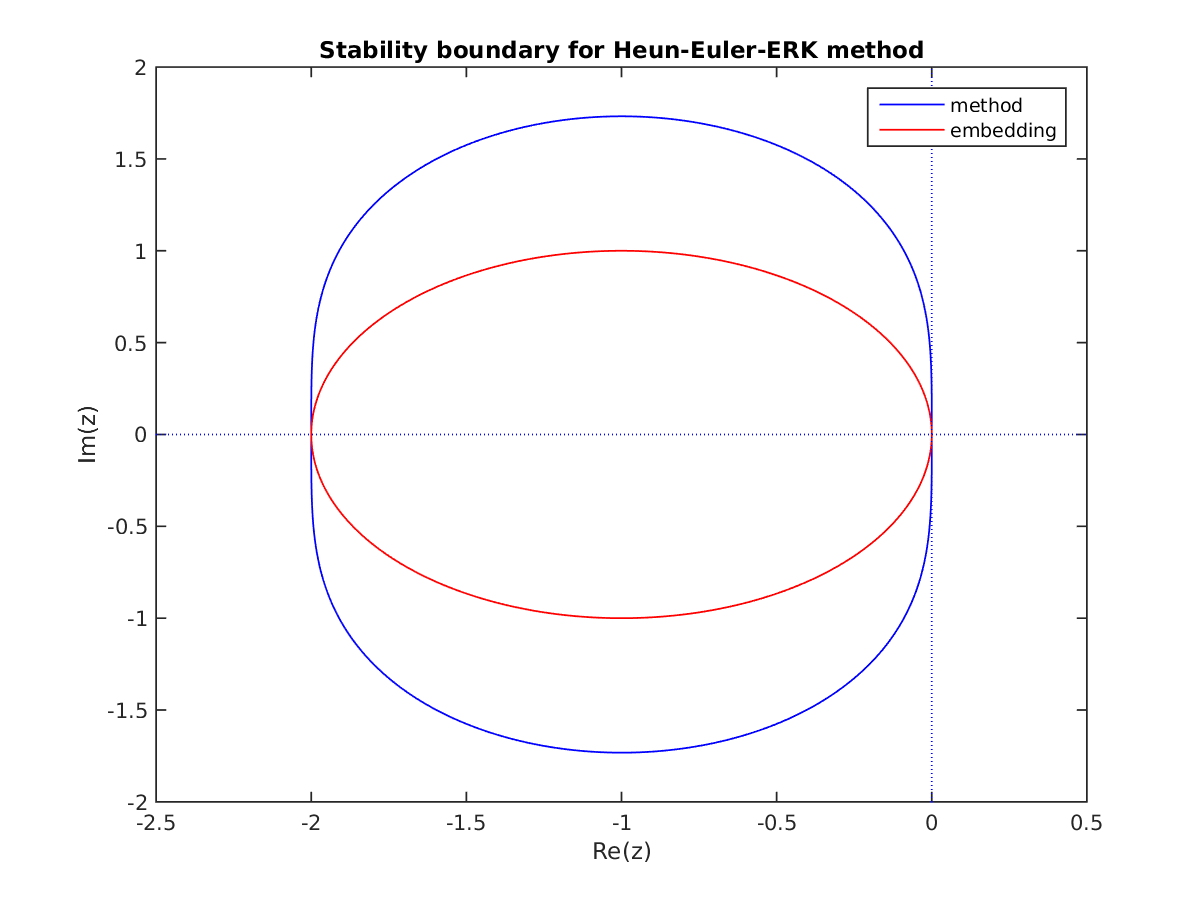
\includegraphics{stab_region_0.png}}
\caption{Linear stability region for the Heun-Euler method.  The method's
region is outlined in blue; the embedding's region is in red.}\end{figure}


\subsection{Bogacki-Shampine-4-2-3}
\label{Butcher:bogacki-shampine-4-2-3}\label{Butcher:butcher-bogacki-shampine}
\index{Bogacki-Shampine-4-2-3 ERK method}
Accessible via the constant \code{BOGACKI\_SHAMPINE\_4\_2\_3} to
{\hyperref[ARKStep_c_interface/User_callable:c.ARKStepSetTableNum]{\emph{\code{ARKStepSetTableNum()}}}}, {\hyperref[ERKStep_c_interface/User_callable:c.ERKStepSetTableNum]{\emph{\code{ERKStepSetTableNum()}}}} or
{\hyperref[ARKodeButcherTable:c.ARKodeButcherTable_LoadERK]{\emph{\code{ARKodeButcherTable\_LoadERK()}}}}.  This is the default 3rd order
explicit method (from \phantomsection\label{Butcher:id1}{\hyperref[References:bs1989]{\emph{{[}BS1989{]}}}}).
\begin{gather}
\begin{split}\renewcommand{\arraystretch}{1.5}
\begin{array}{r|cccc}
  0 &   0 & 0 & 0 & 0 \\
  \frac{1}{2} & \frac{1}{2} & 0 & 0 & 0 \\
  \frac{3}{4} & 0 & \frac{3}{4} & 0 & 0 \\
  1   & \frac{2}{9} & \frac{1}{3} & \frac{4}{9} & 0 \\
  \hline
  3 & \frac{2}{9} & \frac{1}{3} & \frac{4}{9} \\
  2 & \frac{7}{24} & \frac{1}{4} & \frac{1}{3} & \frac{1}{8}
\end{array}\end{split}\notag
\end{gather}\begin{figure}[htbp]
\centering
\capstart

\scalebox{0.500000}{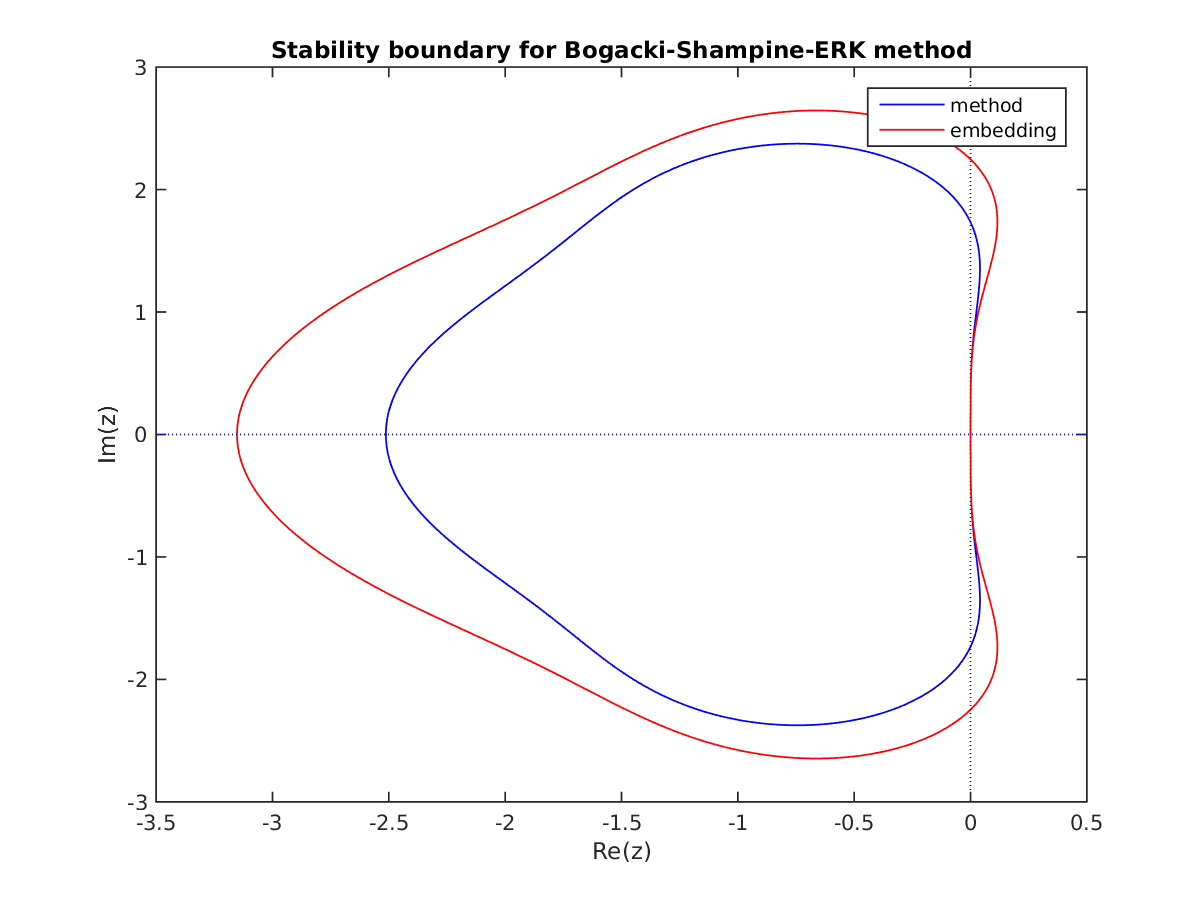
\includegraphics{stab_region_1.png}}
\caption{Linear stability region for the Bogacki-Shampine method.  The method's
region is outlined in blue; the embedding's region is in red.}\end{figure}


\subsection{ARK-4-2-3 (explicit)}
\label{Butcher:butcher-ark-4-2-3-e}\label{Butcher:ark-4-2-3-explicit}
\index{ARK-4-2-3 ERK method}
Accessible via the constant \code{ARK324L2SA\_ERK\_4\_2\_3} to
{\hyperref[ARKStep_c_interface/User_callable:c.ARKStepSetTableNum]{\emph{\code{ARKStepSetTableNum()}}}}, {\hyperref[ERKStep_c_interface/User_callable:c.ERKStepSetTableNum]{\emph{\code{ERKStepSetTableNum()}}}} or
{\hyperref[ARKodeButcherTable:c.ARKodeButcherTable_LoadERK]{\emph{\code{ARKodeButcherTable\_LoadERK()}}}}. This is the explicit portion of
the default 3rd order additive method (from \phantomsection\label{Butcher:id2}{\hyperref[References:kc2003]{\emph{{[}KC2003{]}}}}).
\begin{gather}
\begin{split}\renewcommand{\arraystretch}{1.5}
\begin{array}{r|cccc}
  0 & 0 & 0 & 0 & 0 \\
  \frac{1767732205903}{2027836641118} & \frac{1767732205903}{2027836641118} & 0 & 0 & 0 \\
  \frac{3}{5} & \frac{5535828885825}{10492691773637} & \frac{788022342437}{10882634858940} & 0 & 0 \\
  1 & \frac{6485989280629}{16251701735622} & -\frac{4246266847089}{9704473918619} & \frac{10755448449292}{10357097424841} & 0 \\
  \hline
  3 & \frac{1471266399579}{7840856788654} & -\frac{4482444167858}{7529755066697} & \frac{11266239266428}{11593286722821} & \frac{1767732205903}{4055673282236} \\
  2 & \frac{2756255671327}{12835298489170} & -\frac{10771552573575}{22201958757719} & \frac{9247589265047}{10645013368117} & \frac{2193209047091}{5459859503100}
\end{array}\end{split}\notag
\end{gather}\begin{figure}[htbp]
\centering
\capstart

\scalebox{0.500000}{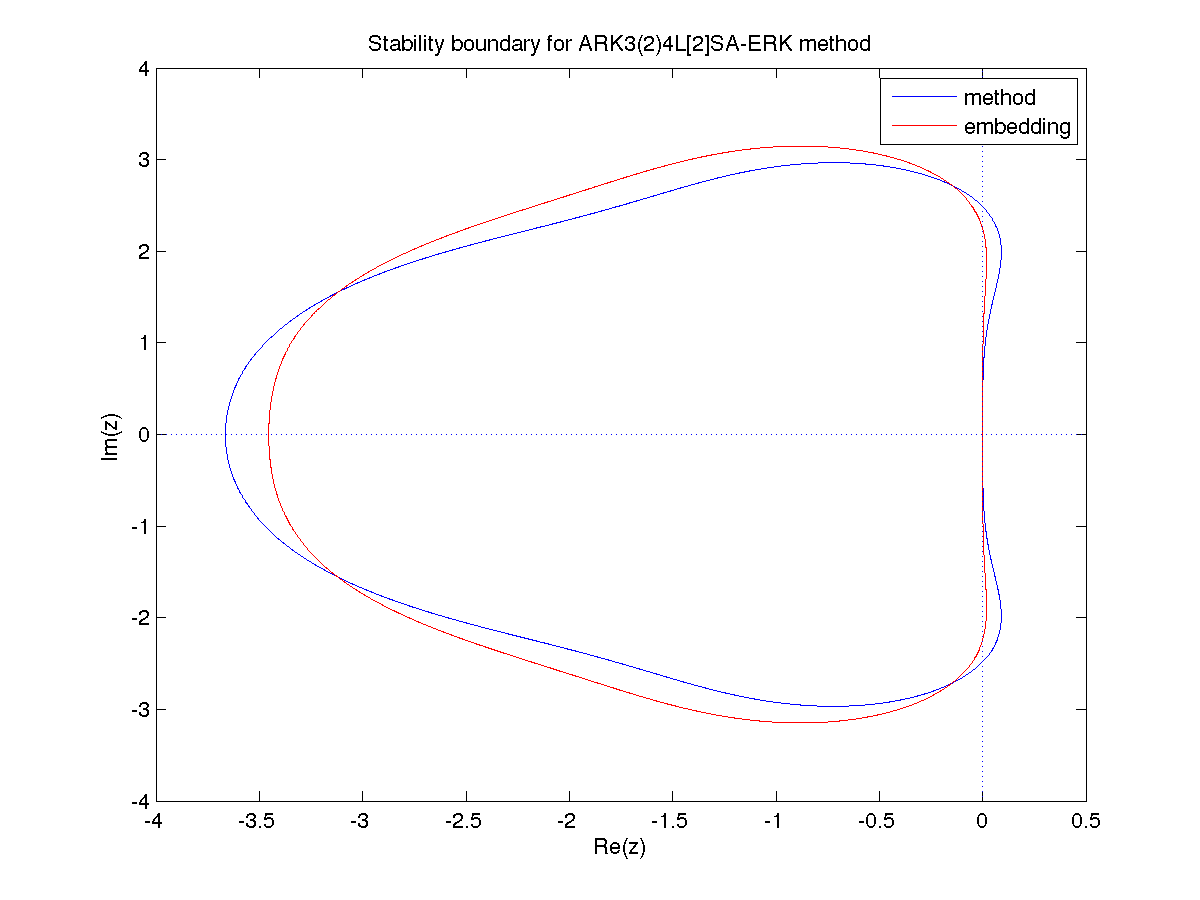
\includegraphics{stab_region_2.png}}
\caption{Linear stability region for the explicit ARK-4-2-3 method.  The method's
region is outlined in blue; the embedding's region is in red.}\end{figure}


\subsection{Knoth-Wolke-3-3}
\label{Butcher:knoth-wolke-3-3}\label{Butcher:butcher-knoth-wolke}
\index{Knoth-Wolke-3-3 ERK method}
Accessible via the constant \code{KNOTH\_WOLKE\_3\_3} to
{\hyperref[MRIStep_c_interface/User_callable:c.MRIStepSetMRITableNum]{\emph{\code{MRIStepSetMRITableNum()}}}} and {\hyperref[ARKodeButcherTable:c.ARKodeButcherTable_LoadERK]{\emph{\code{ARKodeButcherTable\_LoadERK()}}}}.
This is the default 3th order slow and fast MRIStep method (from
\phantomsection\label{Butcher:id3}{\hyperref[References:kw1998]{\emph{{[}KW1998{]}}}}).
\begin{gather}
\begin{split}\renewcommand{\arraystretch}{1.5}
\begin{array}{r|ccc}
            0 & 0             & 0             & 0 \\
  \frac{1}{3} & \frac{1}{3}   & 0             & 0 \\
  \frac{3}{4} & -\frac{3}{16} & \frac{15}{16} & 0 \\
  \hline
            3 & \frac{1}{6} & \frac{3}{10} & \frac{8}{15}
\end{array}\end{split}\notag
\end{gather}\begin{figure}[htbp]
\centering
\capstart

\scalebox{0.500000}{\includegraphics{stab_region_24.png}}
\caption{Linear stability region for the Knoth-Wolke method}\end{figure}


\subsection{Zonneveld-5-3-4}
\label{Butcher:butcher-zonneveld}\label{Butcher:zonneveld-5-3-4}
\index{Zonneveld-5-3-4 ERK method}
Accessible via the constant \code{ZONNEVELD\_5\_3\_4} to
{\hyperref[ARKStep_c_interface/User_callable:c.ARKStepSetTableNum]{\emph{\code{ARKStepSetTableNum()}}}}, {\hyperref[ERKStep_c_interface/User_callable:c.ERKStepSetTableNum]{\emph{\code{ERKStepSetTableNum()}}}}
or {\hyperref[ARKodeButcherTable:c.ARKodeButcherTable_LoadERK]{\emph{\code{ARKodeButcherTable\_LoadERK()}}}}.  This is
the default 4th order explicit method (from \phantomsection\label{Butcher:id4}{\hyperref[References:z1963]{\emph{{[}Z1963{]}}}}).
\begin{gather}
\begin{split}\renewcommand{\arraystretch}{1.5}
\begin{array}{r|ccccc}
    0 & 0 & 0 & 0 & 0 & 0 \\
  \frac{1}{2} & \frac{1}{2} & 0 & 0 & 0 & 0 \\
  \frac{1}{2} & 0 & \frac{1}{2} & 0 & 0 & 0 \\
    1 & 0 & 0 & 1 & 0 & 0 \\
  \frac{3}{4} & \frac{5}{32} & \frac{7}{32} & \frac{13}{32} & -\frac{1}{32} & 0 \\
  \hline
  4 & \frac{1}{6} & \frac{1}{3} & \frac{1}{3} & \frac{1}{6} & 0 \\
  3 & -\frac{1}{2} & \frac{7}{3} & \frac{7}{3} & \frac{13}{6} & -\frac{16}{3}
\end{array}\end{split}\notag
\end{gather}\begin{figure}[htbp]
\centering
\capstart

\scalebox{0.500000}{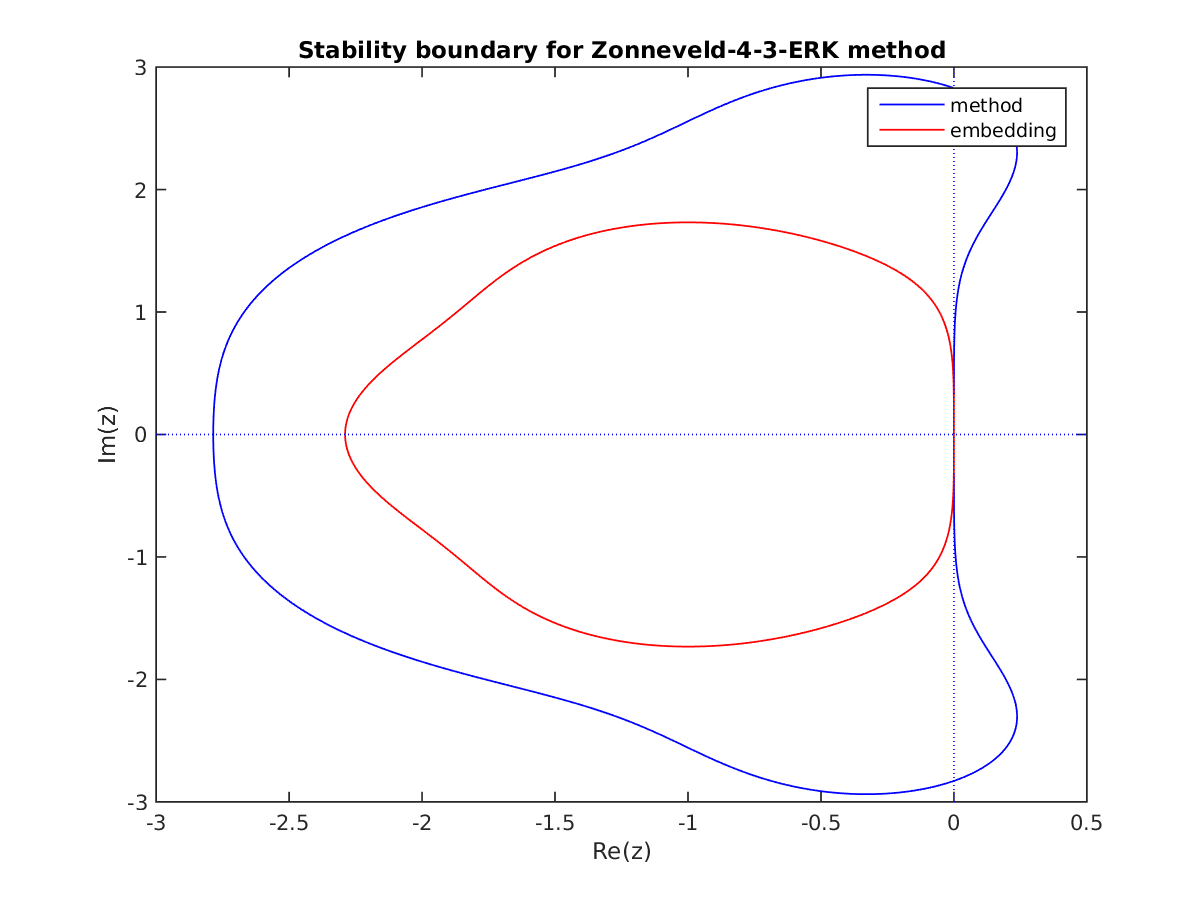
\includegraphics{stab_region_3.png}}
\caption{Linear stability region for the Zonneveld method.  The method's
region is outlined in blue; the embedding's region is in red.}\end{figure}


\subsection{ARK-6-3-4 (explicit)}
\label{Butcher:butcher-ark-6-3-4-e}\label{Butcher:ark-6-3-4-explicit}
\index{ARK-6-3-4 ERK method}
Accessible via the constant \code{ARK436L2SA\_ERK\_6\_3\_4} to
{\hyperref[ARKStep_c_interface/User_callable:c.ARKStepSetTableNum]{\emph{\code{ARKStepSetTableNum()}}}}, {\hyperref[ERKStep_c_interface/User_callable:c.ERKStepSetTableNum]{\emph{\code{ERKStepSetTableNum()}}}}
or {\hyperref[ARKodeButcherTable:c.ARKodeButcherTable_LoadERK]{\emph{\code{ARKodeButcherTable\_LoadERK()}}}}.  This is the explicit portion
of the default 4th order additive method (from \phantomsection\label{Butcher:id5}{\hyperref[References:kc2003]{\emph{{[}KC2003{]}}}}).
\begin{gather}
\begin{split}\renewcommand{\arraystretch}{1.5}
\begin{array}{r|cccccc}
  0 & 0 & 0 & 0 & 0 & 0 & 0 \\
  \frac12 & \frac12 & 0 & 0 & 0 & 0 & 0 \\
  \frac{83}{250} & \frac{13861}{62500} & \frac{6889}{62500} & 0 & 0 & 0 & 0 \\
  \frac{31}{50} & -\frac{116923316275}{2393684061468} & -\frac{2731218467317}{15368042101831} & \frac{9408046702089}{11113171139209} & 0 & 0 & 0 \\
  \frac{17}{20} & -\frac{451086348788}{2902428689909} & -\frac{2682348792572}{7519795681897} & \frac{12662868775082}{11960479115383} & \frac{3355817975965}{11060851509271} & 0 & 0 \\
  1 & \frac{647845179188}{3216320057751} & \frac{73281519250}{8382639484533} & \frac{552539513391}{3454668386233} & \frac{3354512671639}{8306763924573} & \frac{4040}{17871} & 0 \\
  \hline
  4 & \frac{82889}{524892} & 0 & \frac{15625}{83664} & \frac{69875}{102672} & -\frac{2260}{8211} & \frac14 \\
  3 & \frac{4586570599}{29645900160} & 0 & \frac{178811875}{945068544} & \frac{814220225}{1159782912} & -\frac{3700637}{11593932} & \frac{61727}{225920}
\end{array}\end{split}\notag
\end{gather}\begin{figure}[htbp]
\centering
\capstart

\scalebox{0.500000}{\includegraphics{stab_region_4.png}}
\caption{Linear stability region for the explicit ARK-6-3-4 method.  The method's
region is outlined in blue; the embedding's region is in red.}\end{figure}


\subsection{ARK-7-3-4 (explicit)}
\label{Butcher:butcher-ark-7-3-4-e}\label{Butcher:ark-7-3-4-explicit}
\index{ARK-7-3-4 ERK method}
Accessible via the constant \code{ARK437L2SA\_ERK\_7\_3\_4} to
{\hyperref[ARKStep_c_interface/User_callable:c.ARKStepSetTableNum]{\emph{\code{ARKStepSetTableNum()}}}}, {\hyperref[ERKStep_c_interface/User_callable:c.ERKStepSetTableNum]{\emph{\code{ERKStepSetTableNum()}}}}
or {\hyperref[ARKodeButcherTable:c.ARKodeButcherTable_LoadERK]{\emph{\code{ARKodeButcherTable\_LoadERK()}}}}.  This is the explicit portion
of the 4th order additive method (from \phantomsection\label{Butcher:id6}{\hyperref[References:kc2019]{\emph{{[}KC2019{]}}}}).
\begin{gather}
\begin{split}\renewcommand{\arraystretch}{1.5}
\begin{array}{r|ccccccc}
  0 & 0 & 0 & 0 & 0 & 0 & 0 & 0 \\
  \frac{247}{1000} & \frac{247}{1000} & 0 & 0 & 0 & 0 & 0 & 0 \\
  \frac{4276536705230}{10142255878289} & \frac{247}{4000} & \frac{2694949928731}{7487940209513} & 0 & 0 & 0 & 0 & 0 \\
  \frac{67}{200} & \frac{464650059369}{8764239774964} & \frac{878889893998}{2444806327765} & -\frac{952945855348}{12294611323341} & 0 & 0 & 0 & 0 \\
  \frac{3}{40} & \frac{476636172619}{8159180917465} & -\frac{1271469283451}{7793814740893} & -\frac{859560642026}{4356155882851} & \frac{1723805262919}{4571918432560} & 0 & 0 & 0 \\
  \frac{7}{10} & \frac{6338158500785}{11769362343261} & -\frac{4970555480458}{10924838743837} & \frac{3326578051521}{2647936831840} & -\frac{880713585975}{1841400956686} & -\frac{1428733748635}{8843423958496} & 0 & 0 \\
  1 & \frac{760814592956}{3276306540349} & \frac{760814592956}{3276306540349} & -\frac{47223648122716}{6934462133451} & \frac{71187472546993}{9669769126921} & -\frac{13330509492149}{9695768672337} & \frac{11565764226357}{8513123442827} & 0 \\
  \hline
  4 & 0 & 0 & \frac{9164257142617}{17756377923965} & -\frac{10812980402763}{74029279521829} & \frac{1335994250573}{5691609445217} & \frac{2273837961795}{8368240463276} & \frac{247}{2000} \\
  3 & 0 & 0 & \frac{4469248916618}{8635866897933} & -\frac{621260224600}{4094290005349} & \frac{696572312987}{2942599194819} & \frac{1532940081127}{5565293938103} & \frac{2441}{20000}
\end{array}\end{split}\notag
\end{gather}

\subsection{Sayfy-Aburub-6-3-4}
\label{Butcher:butcher-sayfy-aburub}\label{Butcher:sayfy-aburub-6-3-4}
\index{Sayfy-Aburub-6-3-4 ERK method}
Accessible via the constant \code{SAYFY\_ABURUB\_6\_3\_4} to
{\hyperref[ARKStep_c_interface/User_callable:c.ARKStepSetTableNum]{\emph{\code{ARKStepSetTableNum()}}}}, {\hyperref[ERKStep_c_interface/User_callable:c.ERKStepSetTableNum]{\emph{\code{ERKStepSetTableNum()}}}}
or {\hyperref[ARKodeButcherTable:c.ARKodeButcherTable_LoadERK]{\emph{\code{ARKodeButcherTable\_LoadERK()}}}} (from \phantomsection\label{Butcher:id7}{\hyperref[References:sa2002]{\emph{{[}SA2002{]}}}}).
\begin{gather}
\begin{split}\renewcommand{\arraystretch}{1.5}
\begin{array}{r|cccccc}
  0 & 0 & 0 & 0 & 0 & 0 & 0 \\
  \frac{1}{2} & \frac{1}{2} & 0 & 0 & 0 & 0 & 0 \\
  1 & -1 & 2 & 0 & 0 & 0 & 0 \\
  1 & \frac{1}{6} & \frac{2}{3} & \frac{1}{6} & 0 & 0 & 0 \\
  \frac{1}{2} & 0.137 & 0.226 & 0.137 & 0 & 0 & 0 \\
  1 & 0.452 & -0.904 & -0.548 & 0 & 2 & 0 \\
  \hline
  4 & \frac{1}{6} & \frac{1}{3} & \frac{1}{12} & 0 & \frac{1}{3} & \frac{1}{12} \\
  3 & \frac{1}{6} & \frac{2}{3} & \frac{1}{6} & 0 & 0 & 0
\end{array}\end{split}\notag
\end{gather}\begin{figure}[htbp]
\centering
\capstart

\scalebox{0.500000}{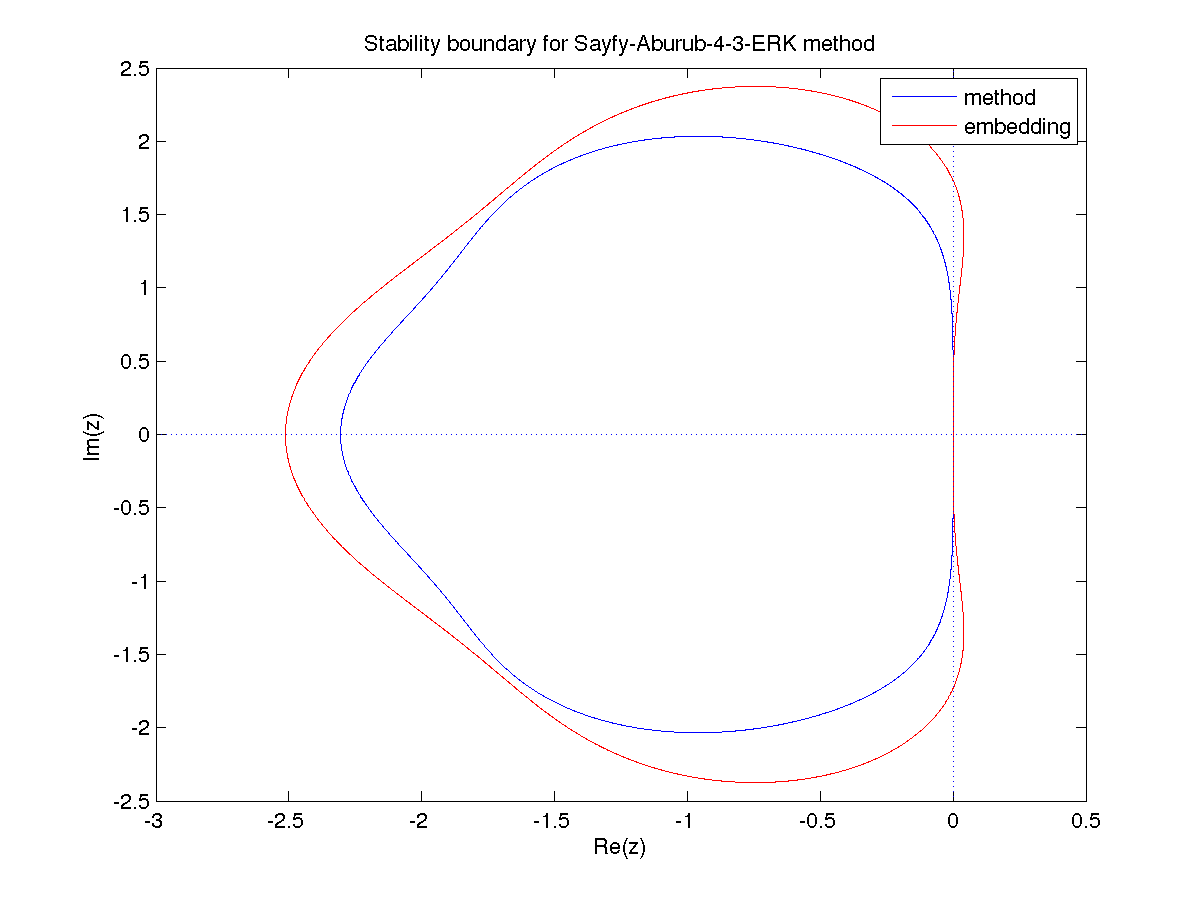
\includegraphics{stab_region_5.png}}
\caption{Linear stability region for the Sayfy-Aburub-6-3-4 method.  The method's
region is outlined in blue; the embedding's region is in red.}\end{figure}


\subsection{Cash-Karp-6-4-5}
\label{Butcher:cash-karp-6-4-5}\label{Butcher:butcher-cash-karp}
\index{Cash-Karp-6-4-5 ERK method}
Accessible via the constant \code{CASH\_KARP\_6\_4\_5} to
{\hyperref[ARKStep_c_interface/User_callable:c.ARKStepSetTableNum]{\emph{\code{ARKStepSetTableNum()}}}}, {\hyperref[ERKStep_c_interface/User_callable:c.ERKStepSetTableNum]{\emph{\code{ERKStepSetTableNum()}}}}
or {\hyperref[ARKodeButcherTable:c.ARKodeButcherTable_LoadERK]{\emph{\code{ARKodeButcherTable\_LoadERK()}}}}.  This is the default 5th order
explicit method (from \phantomsection\label{Butcher:id8}{\hyperref[References:ck1990]{\emph{{[}CK1990{]}}}}).
\begin{gather}
\begin{split}\renewcommand{\arraystretch}{1.5}
\begin{array}{r|cccccc}
  0 & 0 & 0 & 0 & 0 & 0 & 0 \\
  \frac{1}{5} & \frac{1}{5} & 0 & 0 & 0 & 0 & 0 \\
  \frac{3}{10} & \frac{3}{40} & \frac{9}{40} & 0 & 0 & 0 & 0 \\
  \frac{3}{5} & \frac{3}{10} & -\frac{9}{10} & \frac{6}{5} & 0 & 0 & 0 \\
  1 & -\frac{11}{54} & \frac{5}{2} & -\frac{70}{27} & \frac{35}{27} & 0 & 0 \\
  \frac{7}{8} & \frac{1631}{55296} & \frac{175}{512} & \frac{575}{13824} & \frac{44275}{110592} & \frac{253}{4096} & 0 \\
  \hline
  5 & \frac{37}{378} & 0 & \frac{250}{621} & \frac{125}{594} & 0 & \frac{512}{1771} \\
  4 & \frac{2825}{27648} & 0 & \frac{18575}{48384} & \frac{13525}{55296} & \frac{277}{14336} & \frac{1}{4}
\end{array}\end{split}\notag
\end{gather}\begin{figure}[htbp]
\centering
\capstart

\scalebox{0.500000}{\includegraphics{stab_region_6.png}}
\caption{Linear stability region for the Cash-Karp method.  The method's
region is outlined in blue; the embedding's region is in red.}\end{figure}


\subsection{Fehlberg-6-4-5}
\label{Butcher:butcher-fehlberg}\label{Butcher:fehlberg-6-4-5}
\index{Fehlberg-6-4-5 ERK method}
Accessible via the constant \code{FEHLBERG\_6\_4\_5} to
{\hyperref[ARKStep_c_interface/User_callable:c.ARKStepSetTableNum]{\emph{\code{ARKStepSetTableNum()}}}}, {\hyperref[ERKStep_c_interface/User_callable:c.ERKStepSetTableNum]{\emph{\code{ERKStepSetTableNum()}}}}
or {\hyperref[ARKodeButcherTable:c.ARKodeButcherTable_LoadERK]{\emph{\code{ARKodeButcherTable\_LoadERK()}}}} (from \phantomsection\label{Butcher:id9}{\hyperref[References:f1969]{\emph{{[}F1969{]}}}}).
\begin{gather}
\begin{split}\renewcommand{\arraystretch}{1.5}
\begin{array}{r|cccccc}
  0 & 0 & 0 & 0 & 0 & 0 & 0 \\
  \frac{1}{4} & \frac{1}{4} & 0 & 0 & 0 & 0 & 0 \\
  \frac{3}{8} & \frac{3}{32} & \frac{9}{32} & 0 & 0 & 0 & 0 \\
  \frac{12}{13} & \frac{1932}{2197} & -\frac{7200}{2197} & \frac{7296}{2197} & 0 & 0 & 0 \\
  1 & \frac{439}{216} & -8 & \frac{3680}{513} & -\frac{845}{4104} & 0 & 0 \\
  \frac{1}{2} & -\frac{8}{27} & 2 & -\frac{3544}{2565} & \frac{1859}{4104} & -\frac{11}{40} & 0 \\
  \hline
  5 & \frac{16}{135} & 0 & \frac{6656}{12825} & \frac{28561}{56430} & -\frac{9}{50} & \frac{2}{55} \\
  4 & \frac{25}{216} & 0 & \frac{1408}{2565} & \frac{2197}{4104} & -\frac{1}{5} & 0
\end{array}\end{split}\notag
\end{gather}\begin{figure}[htbp]
\centering
\capstart

\scalebox{0.500000}{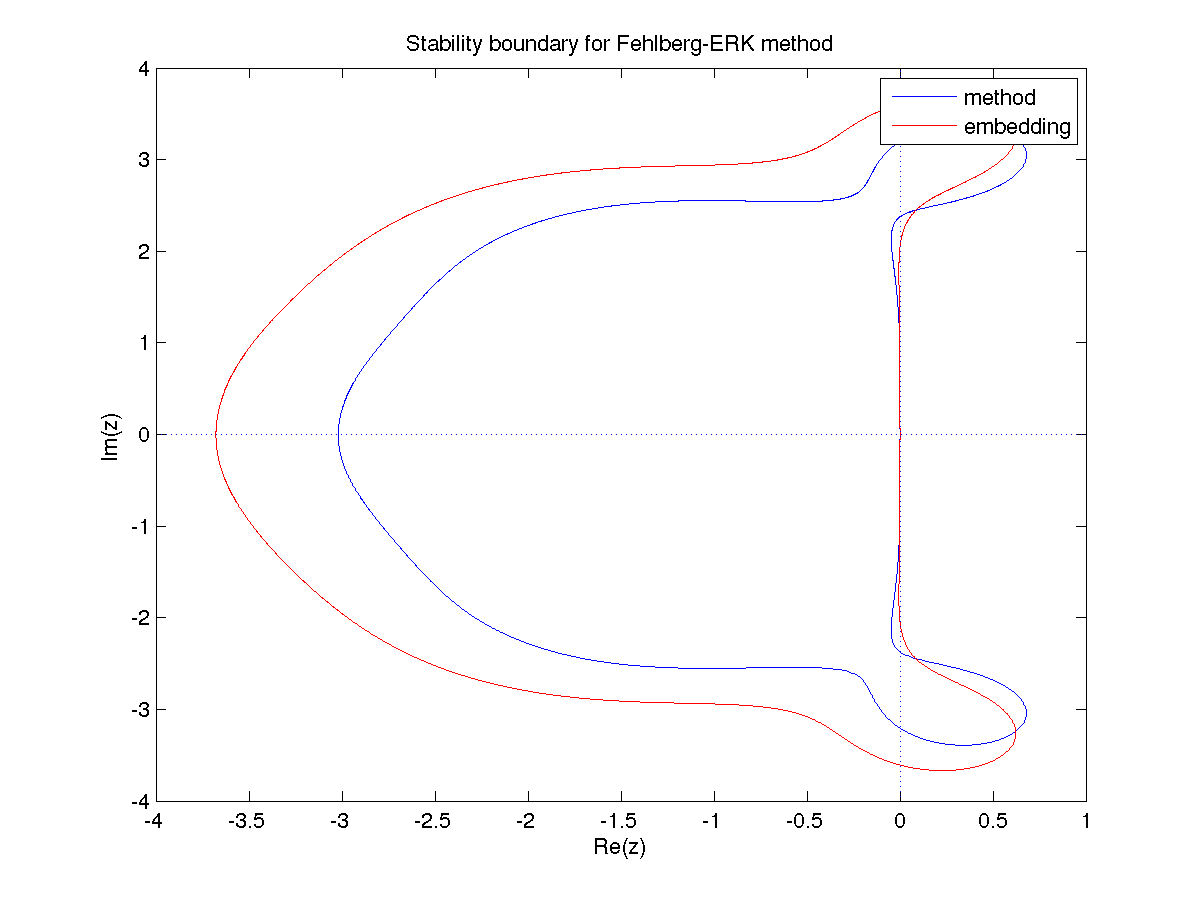
\includegraphics{stab_region_7.png}}
\caption{Linear stability region for the Fehlberg method.  The method's
region is outlined in blue; the embedding's region is in red.}\end{figure}


\subsection{Dormand-Prince-7-4-5}
\label{Butcher:dormand-prince-7-4-5}\label{Butcher:butcher-dormand-prince}
\index{Dormand-Prince-7-4-5 ERK method}
Accessible via the constant \code{DORMAND\_PRINCE\_7\_4\_5} to
{\hyperref[ARKStep_c_interface/User_callable:c.ARKStepSetTableNum]{\emph{\code{ARKStepSetTableNum()}}}}, {\hyperref[ERKStep_c_interface/User_callable:c.ERKStepSetTableNum]{\emph{\code{ERKStepSetTableNum()}}}}
or {\hyperref[ARKodeButcherTable:c.ARKodeButcherTable_LoadERK]{\emph{\code{ARKodeButcherTable\_LoadERK()}}}} (from \phantomsection\label{Butcher:id10}{\hyperref[References:dp1980]{\emph{{[}DP1980{]}}}}).
\begin{gather}
\begin{split}\renewcommand{\arraystretch}{1.5}
\begin{array}{r|ccccccc}
  0 & 0 & 0 & 0 & 0 & 0 & 0 & 0 \\
  \frac{1}{5} & \frac{1}{5} & 0 & 0 & 0 & 0 & 0 & 0 \\
  \frac{3}{10} & \frac{3}{40} & \frac{9}{40} & 0 & 0 & 0 & 0 & 0 \\
  \frac{4}{5} & \frac{44}{45} & -\frac{56}{15} & \frac{32}{9} & 0 & 0 & 0 & 0 \\
  \frac{8}{9} & \frac{19372}{6561} & -\frac{25360}{2187} & \frac{64448}{6561} & -\frac{212}{729} & 0 & 0 & 0 \\
  1 & \frac{9017}{3168} & -\frac{355}{33} & \frac{46732}{5247} & \frac{49}{176} & -\frac{5103}{18656} & 0 & 0 \\
  1 & \frac{35}{384} & 0 & \frac{500}{1113} & \frac{125}{192} & -\frac{2187}{6784} & \frac{11}{84} & 0 \\
  \hline
  5 & \frac{35}{384} & 0 & \frac{500}{1113} & \frac{125}{192} & -\frac{2187}{6784} & \frac{11}{84} & 0 \\
  4 & \frac{5179}{57600} & 0 & \frac{7571}{16695} & \frac{393}{640} & -\frac{92097}{339200} & \frac{187}{2100} & \frac{1}{40}
\end{array}\end{split}\notag
\end{gather}\begin{figure}[htbp]
\centering
\capstart

\scalebox{0.500000}{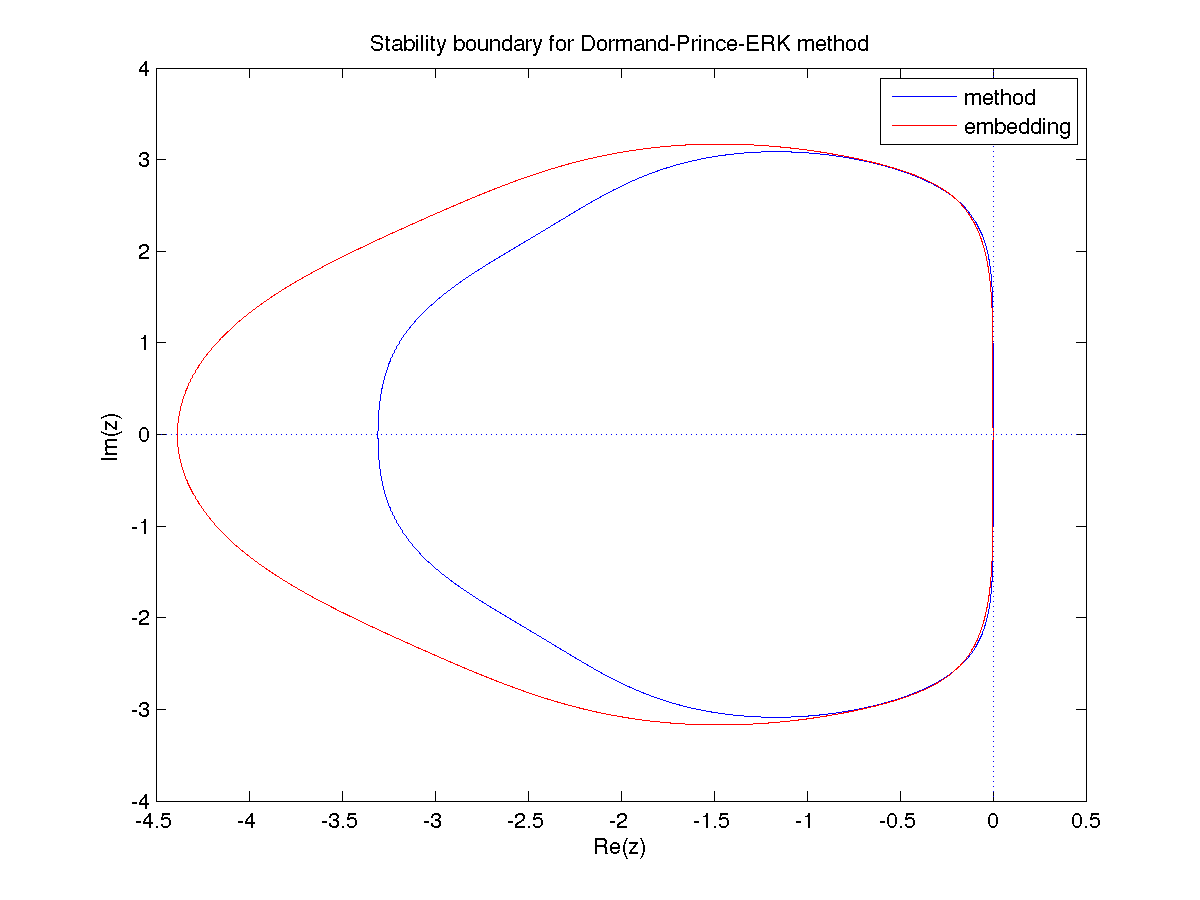
\includegraphics{stab_region_8.png}}
\caption{Linear stability region for the Dormand-Prince method.  The method's
region is outlined in blue; the embedding's region is in red.}\end{figure}


\subsection{ARK-8-4-5 (explicit)}
\label{Butcher:butcher-ark-8-4-5-e}\label{Butcher:ark-8-4-5-explicit}
\index{ARK-8-4-5 ERK method}
Accessible via the constant \code{ARK548L2SA\_ERK\_8\_4\_5} to
{\hyperref[ARKStep_c_interface/User_callable:c.ARKStepSetTableNum]{\emph{\code{ARKStepSetTableNum()}}}}, {\hyperref[ERKStep_c_interface/User_callable:c.ERKStepSetTableNum]{\emph{\code{ERKStepSetTableNum()}}}}
or {\hyperref[ARKodeButcherTable:c.ARKodeButcherTable_LoadERK]{\emph{\code{ARKodeButcherTable\_LoadERK()}}}}.  This is the explicit portion
of the default 5th order additive method (from \phantomsection\label{Butcher:id11}{\hyperref[References:kc2003]{\emph{{[}KC2003{]}}}}).
\begin{gather}
\begin{split}\renewcommand{\arraystretch}{1.5}
\begin{array}{r|cccccccc}
  0 & 0 & 0 & 0 & 0 & 0 & 0 & 0 & 0 \\
  \frac{41}{100} & \frac{41}{100} & 0 & 0 & 0 & 0 & 0 & 0 & 0 \\
  \frac{2935347310677}{11292855782101} & \frac{367902744464}{2072280473677} & \frac{677623207551}{8224143866563} & 0 & 0 & 0 & 0 & 0 & 0 \\
  \frac{1426016391358}{7196633302097} & \frac{1268023523408}{10340822734521} & 0 & \frac{1029933939417}{13636558850479} & 0 & 0 & 0 & 0 & 0 \\
  \frac{92}{100} & \frac{14463281900351}{6315353703477} & 0 & \frac{66114435211212}{5879490589093} & -\frac{54053170152839}{4284798021562} & 0 & 0 & 0 & 0 \\
  \frac{24}{100} & \frac{14090043504691}{34967701212078} & 0 & \frac{15191511035443}{11219624916014} & -\frac{18461159152457}{12425892160975} & -\frac{281667163811}{9011619295870} & 0 & 0 & 0 \\
  \frac{3}{5} & \frac{19230459214898}{13134317526959} & 0 & \frac{21275331358303}{2942455364971} & -\frac{38145345988419}{4862620318723} & -\frac{1}{8} & -\frac{1}{8} & 0 & 0 \\
  1 & -\frac{19977161125411}{11928030595625} & 0 & -\frac{40795976796054}{6384907823539} & \frac{177454434618887}{12078138498510} & \frac{782672205425}{8267701900261} & -\frac{69563011059811}{9646580694205} & \frac{7356628210526}{4942186776405} & 0 \\
  \hline
  5 & -\frac{872700587467}{9133579230613} & 0 & 0 & \frac{22348218063261}{9555858737531} & -\frac{1143369518992}{8141816002931} & -\frac{39379526789629}{19018526304540} & \frac{32727382324388}{42900044865799} & \frac{41}{200} \\
  4 & -\frac{975461918565}{9796059967033} & 0 & 0 & \frac{78070527104295}{32432590147079} & -\frac{548382580838}{3424219808633} & -\frac{33438840321285}{15594753105479} & \frac{3629800801594}{4656183773603} & \frac{4035322873751}{18575991585200}
\end{array}\end{split}\notag
\end{gather}\begin{figure}[htbp]
\centering
\capstart

\scalebox{0.500000}{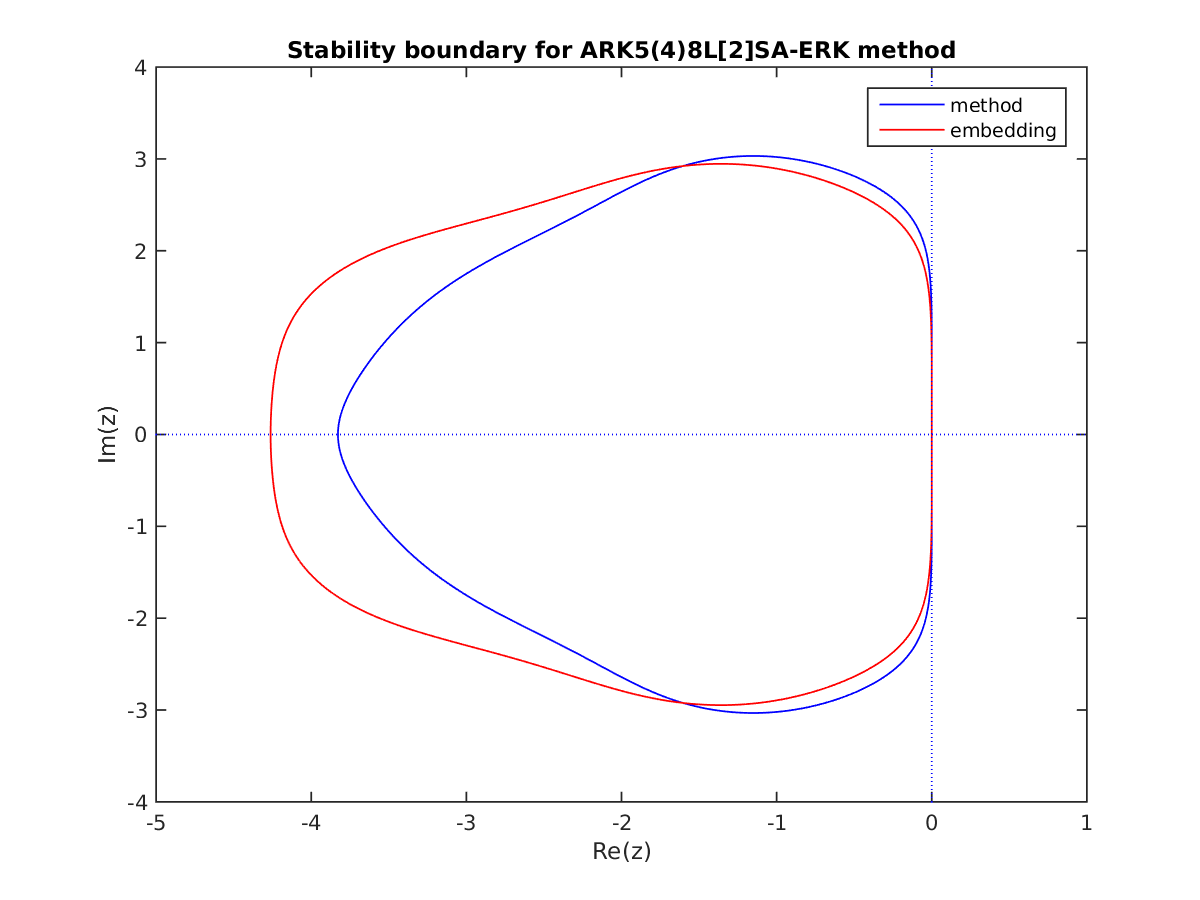
\includegraphics{stab_region_9.png}}
\caption{Linear stability region for the explicit ARK-8-4-5 method.  The method's
region is outlined in blue; the embedding's region is in red.}\end{figure}


\subsection{ARK-8-4-5b (explicit)}
\label{Butcher:butcher-ark-8-4-5b-e}\label{Butcher:ark-8-4-5b-explicit}
\index{ARK-8-4-5b ERK method}
Accessible via the constant \code{ARK548L2SAb\_ERK\_8\_4\_5} to
{\hyperref[ARKStep_c_interface/User_callable:c.ARKStepSetTableNum]{\emph{\code{ARKStepSetTableNum()}}}}, {\hyperref[ERKStep_c_interface/User_callable:c.ERKStepSetTableNum]{\emph{\code{ERKStepSetTableNum()}}}}
or {\hyperref[ARKodeButcherTable:c.ARKodeButcherTable_LoadERK]{\emph{\code{ARKodeButcherTable\_LoadERK()}}}}.  This is the explicit portion
of the 5th order additive method from \phantomsection\label{Butcher:id12}{\hyperref[References:kc2019]{\emph{{[}KC2019{]}}}}.
\begin{gather}
\begin{split}\renewcommand{\arraystretch}{1.5}
\begin{array}{r|cccccccc}
  0 & 0 & 0 & 0 & 0 & 0 & 0 & 0 & 0 \\
  \frac{4}{9} & \frac{4}{9} & 0 & 0 & 0 & 0 & 0 & 0 & 0 \\
  \frac{6456083330201}{8509243623797} & \frac{1}{9} & \frac{1183333538310}{1827251437969} & 0 & 0 & 0 & 0 & 0 & 0 \\
  \frac{1632083962415}{14158861528103} & \frac{895379019517}{9750411845327} & \frac{477606656805}{13473228687314} & \frac{-112564739183}{9373365219272} & 0 & 0 & 0 & 0 & 0 \\
  \frac{6365430648612}{17842476412687} & \frac{-4458043123994}{13015289567637} & \frac{-2500665203865}{9342069639922} & \frac{983347055801}{8893519644487} & \frac{2185051477207}{2551468980502} & 0 & 0 & 0 & 0 \\
  \frac{18}{25} & \frac{-167316361917}{17121522574472} & \frac{1605541814917}{7619724128744} & \frac{991021770328}{13052792161721} & \frac{2342280609577}{11279663441611} & \frac{3012424348531}{12792462456678} & 0 & 0 & 0 \\
  \frac{191}{200} & \frac{6680998715867}{14310383562358} & \frac{5029118570809}{3897454228471} & \frac{2415062538259}{6382199904604} & \frac{-3924368632305}{6964820224454} & \frac{-4331110370267}{15021686902756} & \frac{-3944303808049}{11994238218192} & 0 & 0 \\
  1 & \frac{2193717860234}{3570523412979} & \frac{2193717860234}{3570523412979} & \frac{5952760925747}{18750164281544} & \frac{-4412967128996}{6196664114337} & \frac{4151782504231}{36106512998704} & \frac{572599549169}{6265429158920} & \frac{-457874356192}{11306498036315} & 0 \\
  \hline
  5 & 0 & 0 & \frac{3517720773327}{20256071687669} & \frac{4569610470461}{17934693873752} & \frac{2819471173109}{11655438449929} & \frac{3296210113763}{10722700128969} & \frac{-1142099968913}{5710983926999} & \frac{2}{9} \\
  4 & 0 & 0 & \frac{520639020421}{8300446712847} & \frac{4550235134915}{17827758688493} & \frac{1482366381361}{6201654941325} & \frac{5551607622171}{13911031047899} & \frac{-5266607656330}{36788968843917} & \frac{1074053359553}{5740751784926}
\end{array}\end{split}\notag
\end{gather}

\subsection{Verner-8-5-6}
\label{Butcher:butcher-verner-6-5}\label{Butcher:verner-8-5-6}
\index{Verner-8-5-6 ERK method}
Accessible via the constant \code{VERNER\_8\_5\_6} to
{\hyperref[ARKStep_c_interface/User_callable:c.ARKStepSetTableNum]{\emph{\code{ARKStepSetTableNum()}}}}, {\hyperref[ERKStep_c_interface/User_callable:c.ERKStepSetTableNum]{\emph{\code{ERKStepSetTableNum()}}}}
or {\hyperref[ARKodeButcherTable:c.ARKodeButcherTable_LoadERK]{\emph{\code{ARKodeButcherTable\_LoadERK()}}}}.  This is the default 6th order
explicit method (from \phantomsection\label{Butcher:id13}{\hyperref[References:v1978]{\emph{{[}V1978{]}}}}).
\begin{gather}
\begin{split}\renewcommand{\arraystretch}{1.5}
\begin{array}{r|cccccccc}
  0 & 0 & 0 & 0 & 0 & 0 & 0 & 0 & 0 \\
  \frac{1}{6} & \frac{1}{6} & 0 & 0 & 0 & 0 & 0 & 0 & 0 \\
  \frac{4}{15} & \frac{4}{75} & \frac{16}{75} & 0 & 0 & 0 & 0 & 0 & 0 \\
  \frac{2}{3} & \frac{5}{6} & -\frac{8}{3} & \frac{5}{2} & 0 & 0 & 0 & 0 & 0 \\
  \frac{5}{6} & -\frac{165}{64} & \frac{55}{6} & -\frac{425}{64} & \frac{85}{96} & 0 & 0 & 0 & 0 \\
  1 & \frac{12}{5} & -8 & \frac{4015}{612} & -\frac{11}{36} & \frac{88}{255} & 0 & 0 & 0 \\
  \frac{1}{15} & -\frac{8263}{15000} & \frac{124}{75} & -\frac{643}{680} & -\frac{81}{250} & \frac{2484}{10625} & 0 & 0 & 0 \\
  1 & \frac{3501}{1720} & -\frac{300}{43} & \frac{297275}{52632} & -\frac{319}{2322} & \frac{24068}{84065} & 0 & \frac{3850}{26703} & 0 \\
  \hline
  6 & \frac{3}{40} & 0 & \frac{875}{2244} & \frac{23}{72} & \frac{264}{1955} & 0 & \frac{125}{11592} & \frac{43}{616} \\
  5 & \frac{13}{160} & 0 & \frac{2375}{5984} & \frac{5}{16} & \frac{12}{85} & \frac{3}{44} & 0 & 0
\end{array}\end{split}\notag
\end{gather}\begin{figure}[htbp]
\centering
\capstart

\scalebox{0.500000}{\includegraphics{stab_region_10.png}}
\caption{Linear stability region for the Verner-8-5-6 method.  The method's
region is outlined in blue; the embedding's region is in red.}\end{figure}


\subsection{Fehlberg-13-7-8}
\label{Butcher:butcher-fehlberg-8-7}\label{Butcher:fehlberg-13-7-8}
\index{Fehlberg-13-7-8 ERK method}
Accessible via the constant \code{FEHLBERG\_13\_7\_8} to
{\hyperref[ARKStep_c_interface/User_callable:c.ARKStepSetTableNum]{\emph{\code{ARKStepSetTableNum()}}}}, {\hyperref[ERKStep_c_interface/User_callable:c.ERKStepSetTableNum]{\emph{\code{ERKStepSetTableNum()}}}}
or {\hyperref[ARKodeButcherTable:c.ARKodeButcherTable_LoadERK]{\emph{\code{ARKodeButcherTable\_LoadERK()}}}}.  This is the default 8th order
explicit method (from \phantomsection\label{Butcher:id14}{\hyperref[References:b2008]{\emph{{[}B2008{]}}}}).
\begin{gather}
\begin{split}\renewcommand{\arraystretch}{1.5}
\begin{array}{r|ccccccccccccc}
  0&   0& 0& 0& 0& 0& 0& 0& 0& 0& 0& 0& 0& 0\\
  \frac{2}{27}&   \frac{2}{27}& 0& 0& 0& 0& 0& 0& 0& 0& 0& 0& 0& 0\\
  \frac{1}{9}&   \frac{1}{36}& \frac{1}{12}& 0& 0& 0& 0& 0& 0& 0& 0& 0& 0& 0\\
  \frac{1}{6}&   \frac{1}{24}& 0& \frac{1}{8}& 0& 0& 0& 0& 0& 0& 0& 0& 0& 0\\
  \frac{5}{12}&   \frac{5}{12}& 0& -\frac{25}{16}& \frac{25}{16}& 0& 0& 0& 0& 0& 0& 0& 0& 0\\
  \frac{1}{2}&   \frac{1}{20}& 0& 0& \frac{1}{4}& \frac{1}{5}& 0& 0& 0& 0& 0& 0& 0& 0\\
  \frac{5}{6}&   -\frac{25}{108}& 0& 0& \frac{125}{108}& -\frac{65}{27}& \frac{125}{54}& 0& 0& 0& 0& 0& 0& 0\\
  \frac{1}{6}&   \frac{31}{300}& 0& 0& 0& \frac{61}{225}& -\frac{2}{9}& \frac{13}{900}& 0& 0& 0& 0& 0& 0\\
  \frac{2}{3}&   2& 0& 0& -\frac{53}{6}& \frac{704}{45}& -\frac{107}{9}& \frac{67}{90}& 3& 0& 0& 0& 0& 0\\
  \frac{1}{3}&   -\frac{91}{108}& 0& 0& \frac{23}{108}& -\frac{976}{135}& \frac{311}{54}& -\frac{19}{60}& \frac{17}{6}& -\frac{1}{12}& 0& 0& 0& 0\\
  1&   \frac{2383}{4100}& 0& 0& -\frac{341}{164}& \frac{4496}{1025}& -\frac{301}{82}& \frac{2133}{4100}& \frac{45}{82}& \frac{45}{164}& \frac{18}{41}& 0& 0& 0\\
  0&   \frac{3}{205}& 0& 0& 0& 0& -\frac{6}{41}& -\frac{3}{205}& -\frac{3}{41}& \frac{3}{41}& \frac{6}{41}& 0& 0& 0\\
  1&   -\frac{1777}{4100}& 0& 0& -\frac{341}{164}& \frac{4496}{1025}& -\frac{289}{82}& \frac{2193}{4100}& \frac{51}{82}& \frac{33}{164}& \frac{12}{41}& 0& 1& 0\\
  \hline
  8& 0& 0& 0& 0& 0& \frac{34}{105}& \frac{9}{35}& \frac{9}{35}& \frac{9}{280}& \frac{9}{280}& 0& \frac{41}{840}& \frac{41}{840} \\
  7& \frac{41}{840}& 0& 0& 0& 0& \frac{34}{105}& \frac{9}{35}& \frac{9}{35}& \frac{9}{280}& \frac{9}{280}& \frac{41}{840}& 0& 0
\end{array}\end{split}\notag
\end{gather}\begin{figure}[htbp]
\centering
\capstart

\scalebox{0.500000}{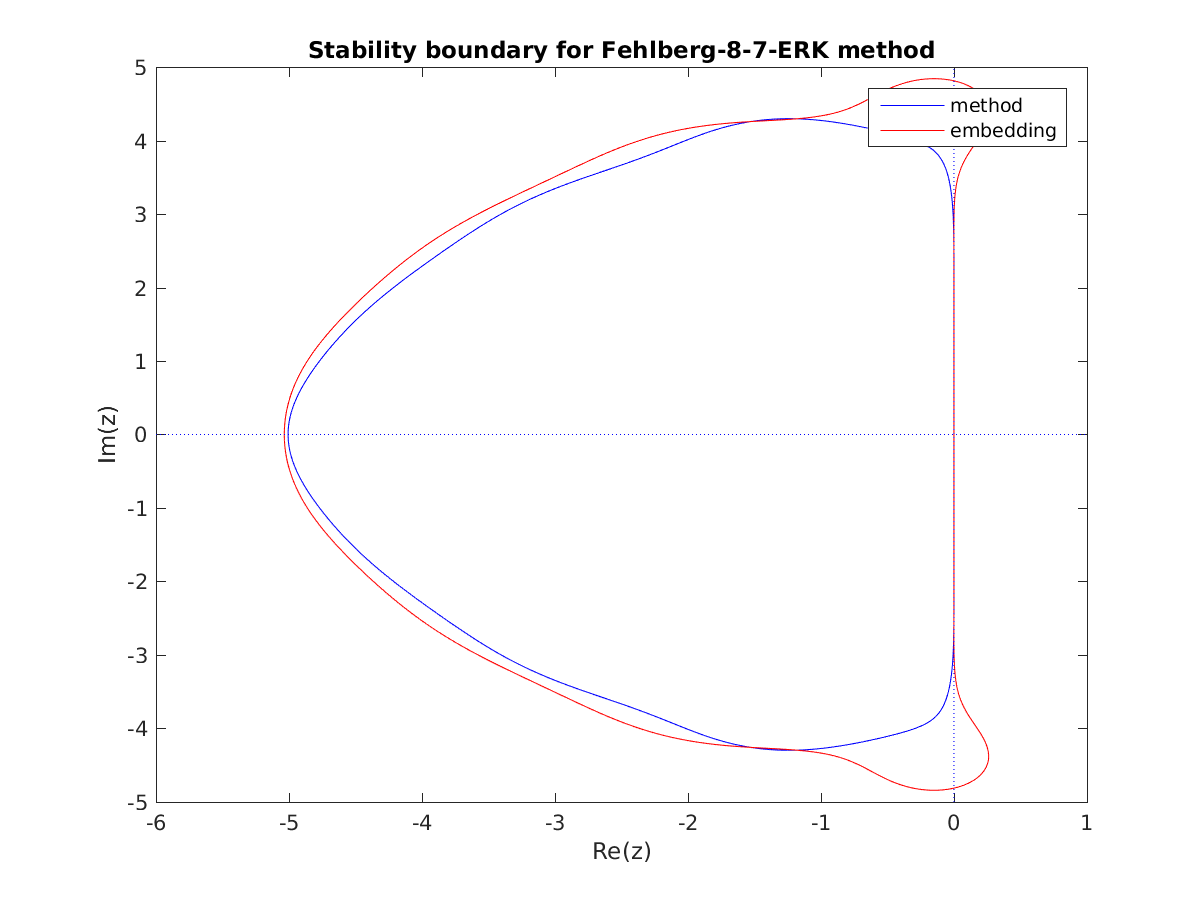
\includegraphics{stab_region_23.png}}
\caption{Linear stability region for the Fehlberg-13-7-8 method.  The method's
region is outlined in blue; the embedding's region is in red.}\end{figure}


\section{Implicit Butcher tables}
\label{Butcher:implicit-butcher-tables}\label{Butcher:butcher-implicit}
In the category of diagonally implicit Runge-Kutta methods, ARKode
includes methods that have orders 2 through 5, with embeddings that are of
orders 1 through 4.


\subsection{SDIRK-2-1-2}
\label{Butcher:sdirk-2-1-2}\label{Butcher:butcher-sdirk-2-1}
\index{SDIRK-2-1-2 method}
Accessible via the constant \code{SDIRK\_2\_1\_2} to
{\hyperref[ARKStep_c_interface/User_callable:c.ARKStepSetTableNum]{\emph{\code{ARKStepSetTableNum()}}}} or
{\hyperref[ARKodeButcherTable:c.ARKodeButcherTable_LoadDIRK]{\emph{\code{ARKodeButcherTable\_LoadDIRK()}}}}.  This is the default 2nd order
implicit method.  Both the method and embedding are A- and B-stable.
\begin{gather}
\begin{split}\renewcommand{\arraystretch}{1.5}
\begin{array}{r|cc}
  1 & 1 & 0 \\
  0 & -1 & 1 \\
  \hline
  2 & \frac{1}{2} & \frac{1}{2} \\
  1 & 1 & 0
\end{array}\end{split}\notag
\end{gather}\begin{figure}[htbp]
\centering
\capstart

\scalebox{0.500000}{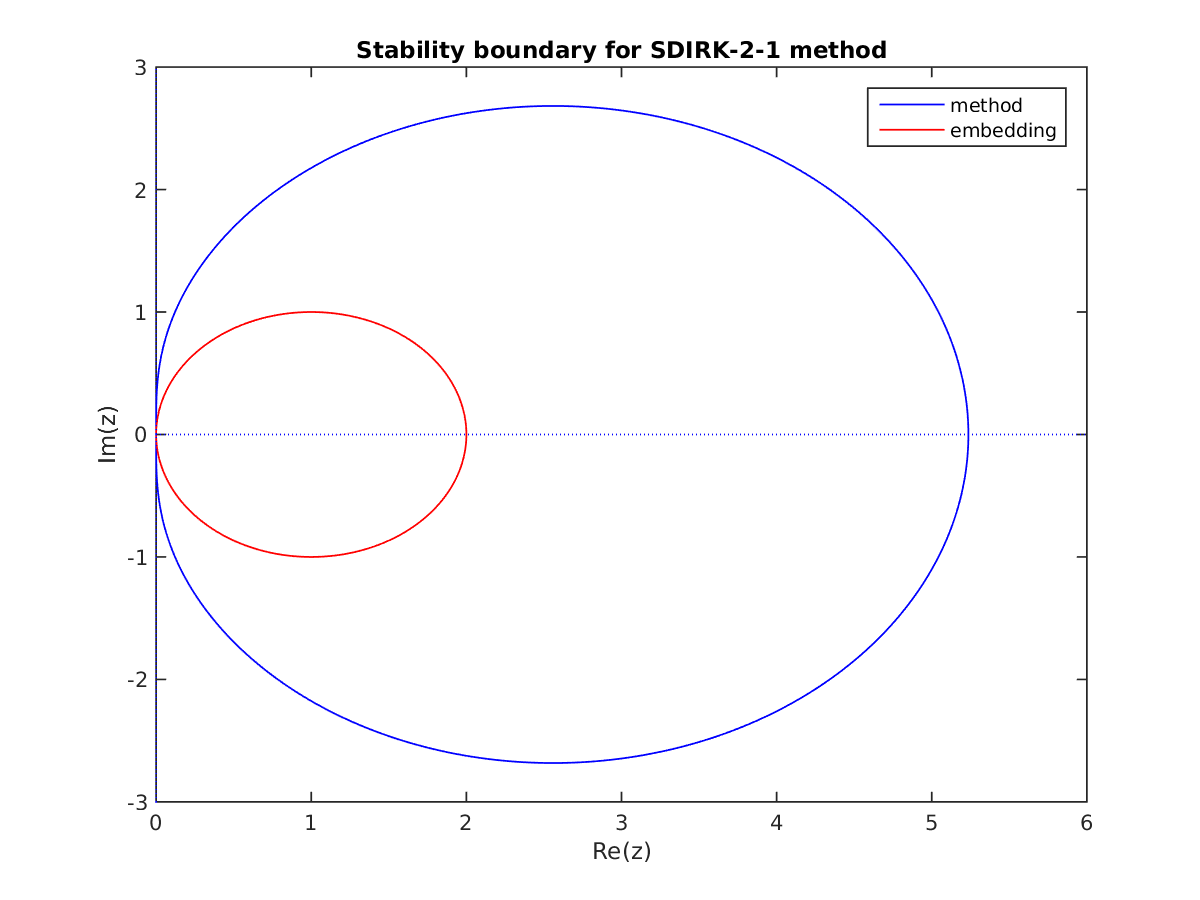
\includegraphics{stab_region_11.png}}
\caption{Linear stability region for the SDIRK-2-1-2 method.  The method's
region is outlined in blue; the embedding's region is in red.}\end{figure}


\subsection{Billington-3-3-2}
\label{Butcher:butcher-billington}\label{Butcher:billington-3-3-2}
\index{Billington-3-3-2 SDIRK method}
Accessible via the constant \code{BILLINGTON\_3\_3\_2} to
{\hyperref[ARKStep_c_interface/User_callable:c.ARKStepSetTableNum]{\emph{\code{ARKStepSetTableNum()}}}} or
{\hyperref[ARKodeButcherTable:c.ARKodeButcherTable_LoadDIRK]{\emph{\code{ARKodeButcherTable\_LoadDIRK()}}}}.  Here, the higher-order
embedding is less stable than the lower-order method (from \phantomsection\label{Butcher:id15}{\hyperref[References:b1983]{\emph{{[}B1983{]}}}}).
\begin{gather}
\begin{split}\renewcommand{\arraystretch}{1.5}
\begin{array}{r|ccc}
  0.292893218813 & 0.292893218813 & 0 & 0 \\
  1.091883092037 & 0.798989873223 & 0.292893218813 & 0 \\
  1.292893218813 & 0.740789228841 & 0.259210771159 & 0.292893218813 \\
  \hline
  2 & 0.740789228840 & 0.259210771159 & 0 \\
  3 & 0.691665115992 & 0.503597029883 & -0.195262145876
\end{array}\end{split}\notag
\end{gather}\begin{figure}[htbp]
\centering
\capstart

\scalebox{0.500000}{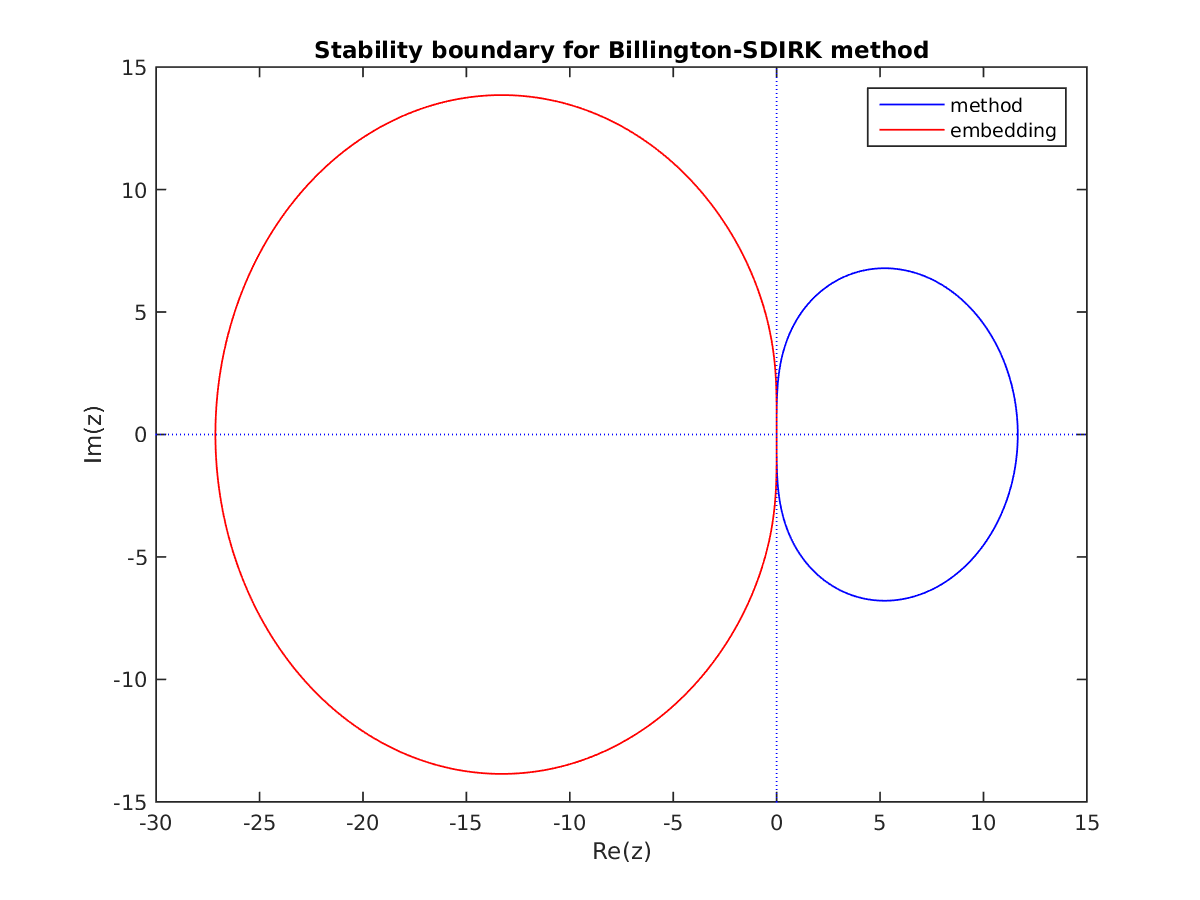
\includegraphics{stab_region_12.png}}
\caption{Linear stability region for the Billington method.  The method's
region is outlined in blue; the embedding's region is in red.}\end{figure}


\subsection{TRBDF2-3-3-2}
\label{Butcher:butcher-trbdf2}\label{Butcher:trbdf2-3-3-2}
\index{TRBDF2-3-3-2 ESDIRK method}
Accessible via the constant \code{TRBDF2\_3\_3\_2} to
{\hyperref[ARKStep_c_interface/User_callable:c.ARKStepSetTableNum]{\emph{\code{ARKStepSetTableNum()}}}} or
{\hyperref[ARKodeButcherTable:c.ARKodeButcherTable_LoadDIRK]{\emph{\code{ARKodeButcherTable\_LoadDIRK()}}}}.  As with Billington, here the
higher-order embedding is less stable than the lower-order method
(from \phantomsection\label{Butcher:id16}{\hyperref[References:b1985]{\emph{{[}B1985{]}}}}).
\begin{gather}
\begin{split}\renewcommand{\arraystretch}{1.5}
\begin{array}{r|ccc}
  0 & 0 & 0 & 0 \\
  2-\sqrt{2} & \frac{2-\sqrt{2}}{2} & \frac{2-\sqrt{2}}{2} & 0 \\
  1 & \frac{\sqrt{2}}{4} & \frac{\sqrt{2}}{4} & \frac{2-\sqrt{2}}{2} \\
  \hline
  2 & \frac{\sqrt{2}}{4} & \frac{\sqrt{2}}{4} & \frac{2-\sqrt{2}}{2} \\
  3 & \frac{1-\frac{\sqrt{2}}{4}}{3} & \frac{\frac{3\sqrt{2}}{4}+1}{3} & \frac{2-\sqrt{2}}{6}
\end{array}\end{split}\notag
\end{gather}\begin{figure}[htbp]
\centering
\capstart

\scalebox{0.500000}{\includegraphics{stab_region_13.png}}
\caption{Linear stability region for the TRBDF2 method.  The method's
region is outlined in blue; the embedding's region is in red.}\end{figure}


\subsection{Kvaerno-4-2-3}
\label{Butcher:butcher-kvaerno-4-2-3}\label{Butcher:kvaerno-4-2-3}
\index{Kvaerno-4-2-3 ESDIRK method}
Accessible via the constant \code{KVAERNO\_4\_2\_3} to
{\hyperref[ARKStep_c_interface/User_callable:c.ARKStepSetTableNum]{\emph{\code{ARKStepSetTableNum()}}}} or
{\hyperref[ARKodeButcherTable:c.ARKodeButcherTable_LoadDIRK]{\emph{\code{ARKodeButcherTable\_LoadDIRK()}}}}.  Both the method and embedding are
A-stable; additionally the method is L-stable (from \phantomsection\label{Butcher:id17}{\hyperref[References:k2004]{\emph{{[}K2004{]}}}}).
\begin{gather}
\begin{split}\renewcommand{\arraystretch}{1.5}
\begin{array}{r|cccc}
  0 & 0 & 0 & 0 & 0 \\
  0.871733043 & 0.4358665215 & 0.4358665215 & 0 & 0 \\
  1 & 0.490563388419108 & 0.073570090080892 & 0.4358665215 & 0 \\
  1 & 0.308809969973036 & 1.490563388254106 & -1.235239879727145 & 0.4358665215 \\
  \hline
  3 & 0.308809969973036 & 1.490563388254106 & -1.235239879727145 & 0.4358665215 \\
  2 & 0.490563388419108 & 0.073570090080892 & 0.4358665215 & 0
\end{array}\end{split}\notag
\end{gather}\begin{figure}[htbp]
\centering
\capstart

\scalebox{0.500000}{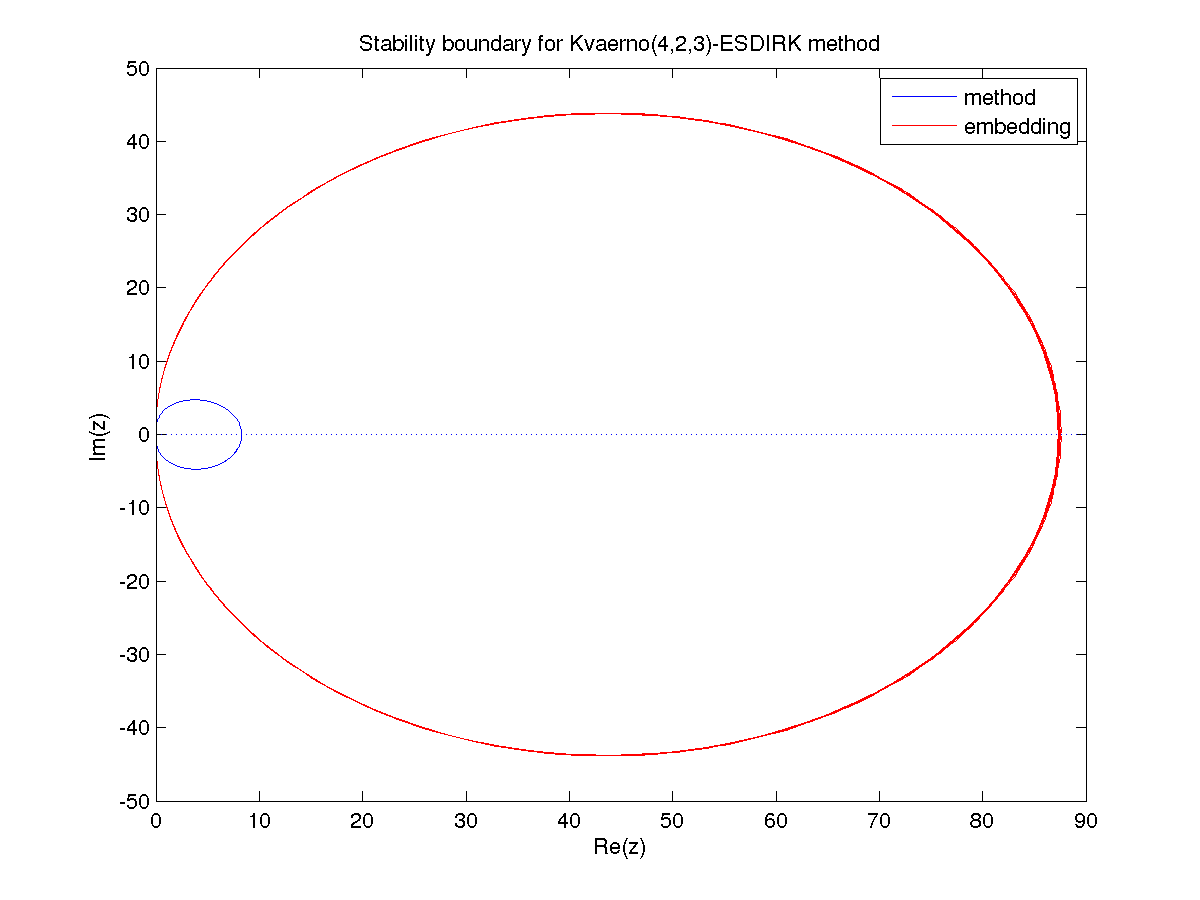
\includegraphics{stab_region_14.png}}
\caption{Linear stability region for the Kvaerno-4-2-3 method.  The method's
region is outlined in blue; the embedding's region is in red.}\end{figure}


\subsection{ARK-4-2-3 (implicit)}
\label{Butcher:ark-4-2-3-implicit}\label{Butcher:butcher-ark-4-2-3-i}
\index{ARK-4-2-3 ESDIRK method}
Accessible via the constant \code{ARK324L2SA\_DIRK\_4\_2\_3} to
{\hyperref[ARKStep_c_interface/User_callable:c.ARKStepSetTableNum]{\emph{\code{ARKStepSetTableNum()}}}} or
{\hyperref[ARKodeButcherTable:c.ARKodeButcherTable_LoadDIRK]{\emph{\code{ARKodeButcherTable\_LoadDIRK()}}}}.  This is the default 3rd order
implicit method, and the implicit portion of the default 3rd order
additive method.  Both the method and embedding are A-stable;
additionally the method is L-stable (from \phantomsection\label{Butcher:id18}{\hyperref[References:kc2003]{\emph{{[}KC2003{]}}}}).
\begin{gather}
\begin{split}\renewcommand{\arraystretch}{1.5}
\begin{array}{r|cccc}
  0 & 0 & 0 & 0 & 0 \\
  \frac{1767732205903}{2027836641118} & \frac{1767732205903}{4055673282236} & \frac{1767732205903}{4055673282236} & 0 & 0 \\
  \frac{3}{5} & \frac{2746238789719}{10658868560708} & -\frac{640167445237}{6845629431997} & \frac{1767732205903}{4055673282236} & 0 \\
  1 & \frac{1471266399579}{7840856788654} & -\frac{4482444167858}{7529755066697} & \frac{11266239266428}{11593286722821} & \frac{1767732205903}{4055673282236} \\
  \hline
  3 & \frac{1471266399579}{7840856788654} & -\frac{4482444167858}{7529755066697} & \frac{11266239266428}{11593286722821} & \frac{1767732205903}{4055673282236} \\
  2 & \frac{2756255671327}{12835298489170} & -\frac{10771552573575}{22201958757719} & \frac{9247589265047}{10645013368117} & \frac{2193209047091}{5459859503100}
\end{array}\end{split}\notag
\end{gather}\begin{figure}[htbp]
\centering
\capstart

\scalebox{0.500000}{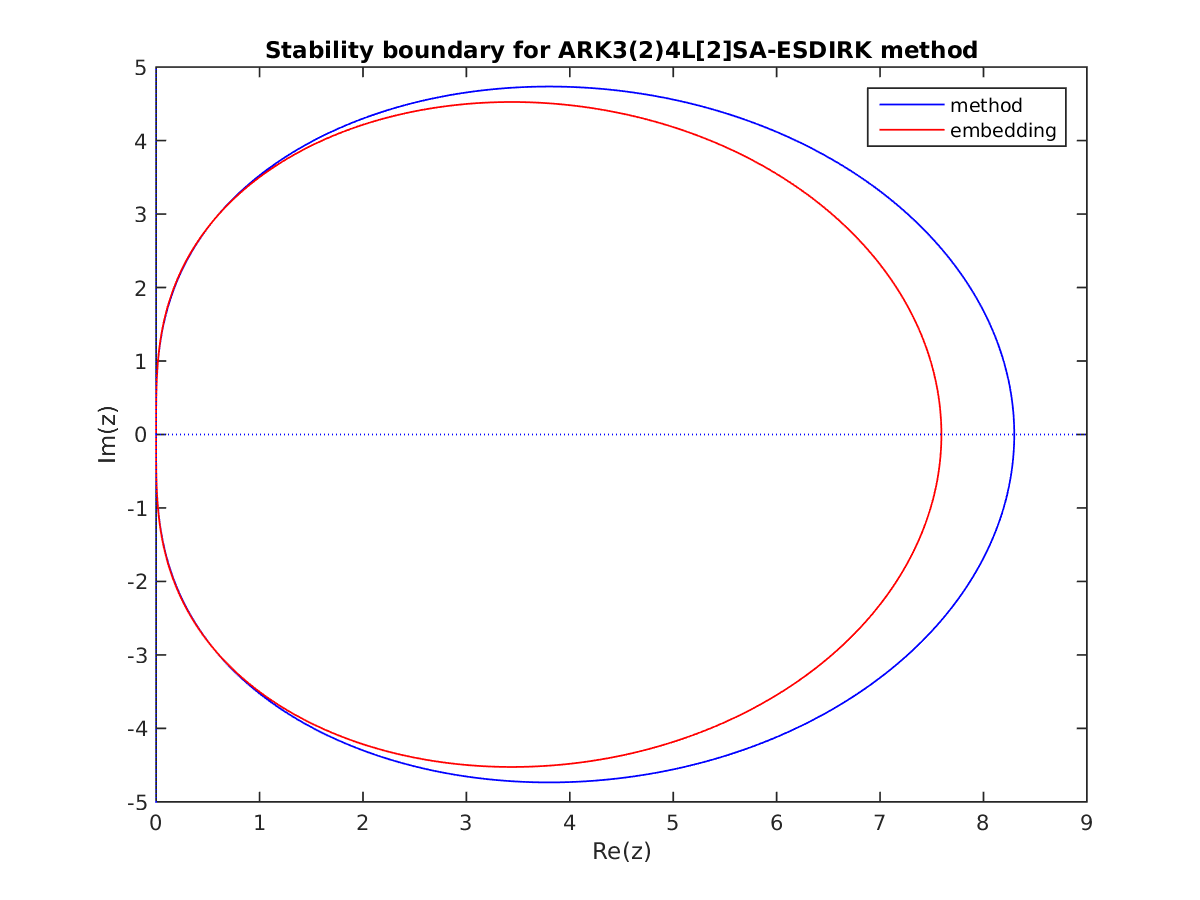
\includegraphics{stab_region_15.png}}
\caption{Linear stability region for the implicit ARK-4-2-3 method.  The method's
region is outlined in blue; the embedding's region is in red.}\end{figure}


\subsection{Cash-5-2-4}
\label{Butcher:butcher-cash-5-2-4}\label{Butcher:cash-5-2-4}
\index{Cash-5-2-4 SDIRK method}
Accessible via the constant \code{CASH\_5\_2\_4} to
{\hyperref[ARKStep_c_interface/User_callable:c.ARKStepSetTableNum]{\emph{\code{ARKStepSetTableNum()}}}} or
{\hyperref[ARKodeButcherTable:c.ARKodeButcherTable_LoadDIRK]{\emph{\code{ARKodeButcherTable\_LoadDIRK()}}}}.  Both the method and embedding are
A-stable; additionally the method is L-stable (from \phantomsection\label{Butcher:id19}{\hyperref[References:c1979]{\emph{{[}C1979{]}}}}).
\begin{gather}
\begin{split}\renewcommand{\arraystretch}{1.5}
\begin{array}{r|ccccc}
  0.435866521508 & 0.435866521508 & 0 & 0 & 0 & 0 \\
  -0.7 & -1.13586652150 & 0.435866521508 & 0 & 0 & 0 \\
  0.8 & 1.08543330679 & -0.721299828287 & 0.435866521508 & 0 & 0 \\
  0.924556761814 & 0.416349501547 & 0.190984004184 & -0.118643265417 & 0.435866521508 & 0 \\
  1 & 0.896869652944 & 0.0182725272734 & -0.0845900310706 & -0.266418670647 & 0.435866521508 \\
  \hline
  4 & 0.896869652944 & 0.0182725272734 & -0.0845900310706 & -0.266418670647 & 0.435866521508 \\
  2 & 1.05646216107052 & -0.0564621610705236 & 0 & 0 & 0
\end{array}\end{split}\notag
\end{gather}\begin{figure}[htbp]
\centering
\capstart

\scalebox{0.500000}{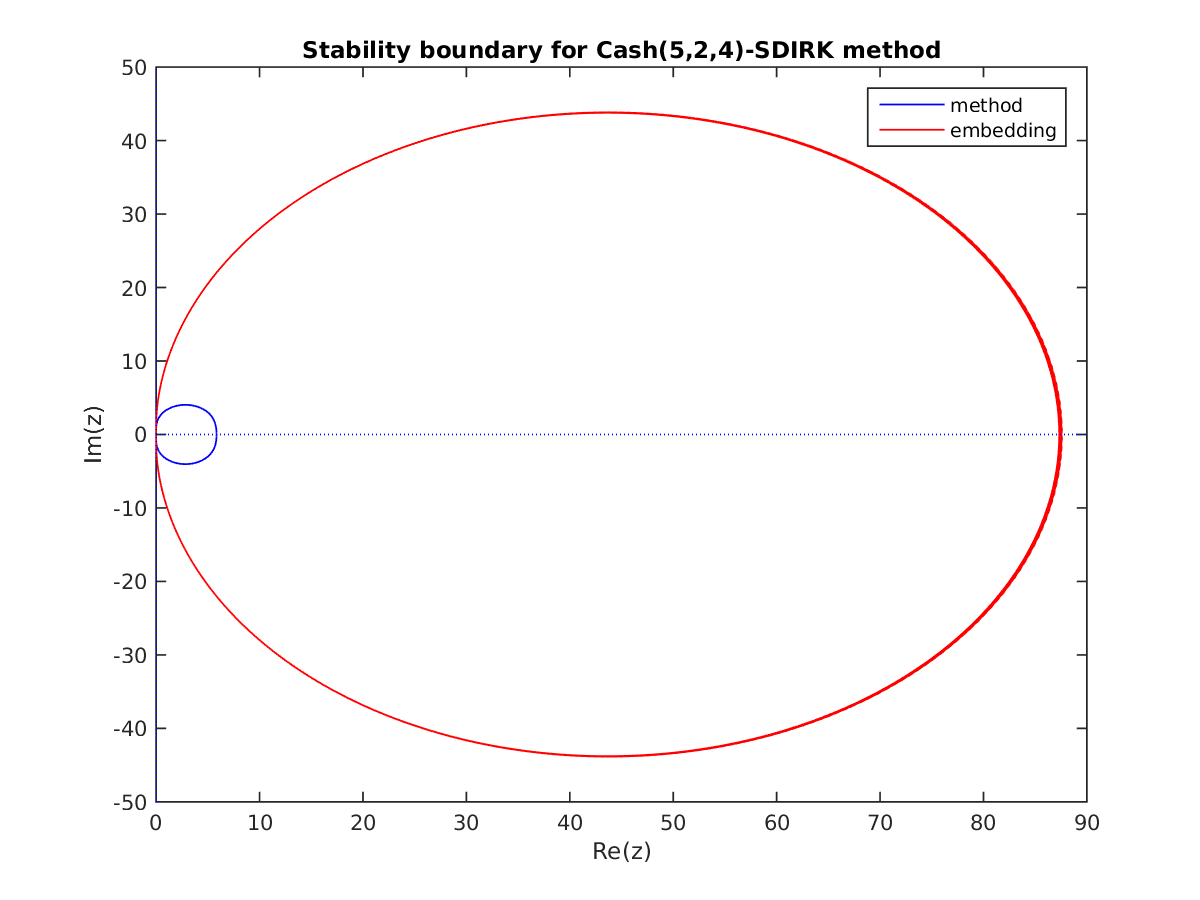
\includegraphics{stab_region_16.png}}
\caption{Linear stability region for the Cash-5-2-4 method.  The method's
region is outlined in blue; the embedding's region is in red.}\end{figure}


\subsection{Cash-5-3-4}
\label{Butcher:butcher-cash-5-3-4}\label{Butcher:cash-5-3-4}
\index{Cash-5-3-4 SDIRK method}
Accessible via the constant \code{CASH\_5\_3\_4} to
{\hyperref[ARKStep_c_interface/User_callable:c.ARKStepSetTableNum]{\emph{\code{ARKStepSetTableNum()}}}} or
{\hyperref[ARKodeButcherTable:c.ARKodeButcherTable_LoadDIRK]{\emph{\code{ARKodeButcherTable\_LoadDIRK()}}}}.  Both the method and embedding are
A-stable; additionally the method is L-stable (from \phantomsection\label{Butcher:id20}{\hyperref[References:c1979]{\emph{{[}C1979{]}}}}).
\begin{gather}
\begin{split}\renewcommand{\arraystretch}{1.5}
\begin{array}{r|ccccc}
  0.435866521508 & 0.435866521508 & 0 & 0 & 0 & 0 \\
  -0.7 & -1.13586652150 & 0.435866521508 & 0 & 0 & 0 \\
  0.8 & 1.08543330679 & -0.721299828287 & 0.435866521508 & 0 & 0 \\
  0.924556761814 & 0.416349501547 & 0.190984004184 & -0.118643265417 & 0.435866521508 & 0 \\
  1 & 0.896869652944 & 0.0182725272734 & -0.0845900310706 & -0.266418670647 & 0.435866521508 \\
  \hline
  4 & 0.896869652944 & 0.0182725272734 & -0.0845900310706 & -0.266418670647 & 0.435866521508 \\
  3 & 0.776691932910 & 0.0297472791484 & -0.0267440239074 & 0.220304811849 & 0
\end{array}\end{split}\notag
\end{gather}\begin{figure}[htbp]
\centering
\capstart

\scalebox{0.500000}{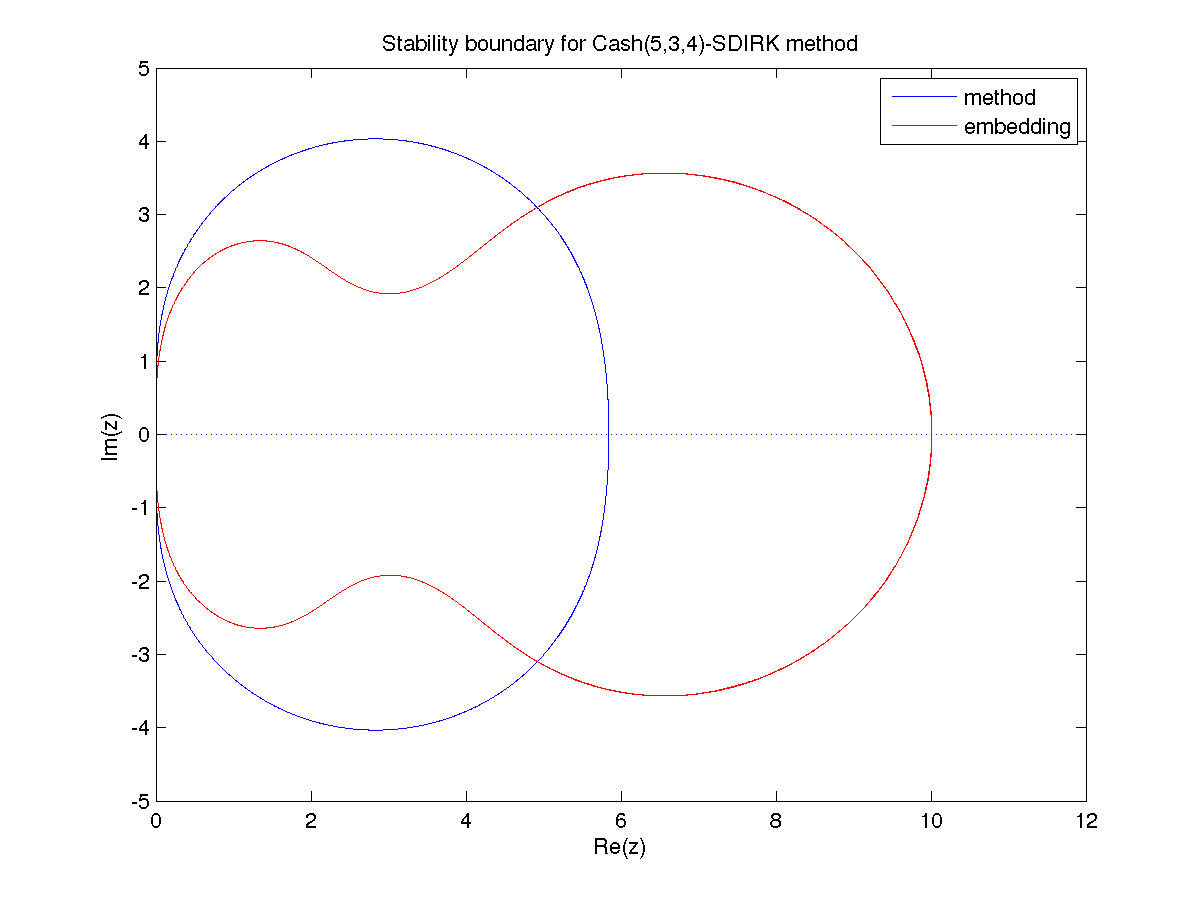
\includegraphics{stab_region_17.png}}
\caption{Linear stability region for the Cash-5-3-4 method.  The method's
region is outlined in blue; the embedding's region is in red.}\end{figure}


\subsection{SDIRK-5-3-4}
\label{Butcher:butcher-sdirk-5-4}\label{Butcher:sdirk-5-3-4}
\index{SDIRK-5-3-4 method}
Accessible via the constant \code{SDIRK\_5\_3\_4} to
{\hyperref[ARKStep_c_interface/User_callable:c.ARKStepSetTableNum]{\emph{\code{ARKStepSetTableNum()}}}} or
{\hyperref[ARKodeButcherTable:c.ARKodeButcherTable_LoadDIRK]{\emph{\code{ARKodeButcherTable\_LoadDIRK()}}}}.  This is the default 4th order
implicit method.  Here, the method is both A- and L-stable, although
the embedding has reduced stability (from \phantomsection\label{Butcher:id21}{\hyperref[References:hw1996]{\emph{{[}HW1996{]}}}}).
\begin{gather}
\begin{split}\renewcommand{\arraystretch}{1.5}
\begin{array}{r|ccccc}
  \frac{1}{4} & \frac{1}{4} & 0 & 0 & 0 & 0 \\
  \frac{3}{4} & \frac{1}{2} & \frac{1}{4} & 0 & 0 & 0 \\
  \frac{11}{20} & \frac{17}{50} & -\frac{1}{25} & \frac{1}{4} & 0 & 0 \\
  \frac{1}{2} & \frac{371}{1360} & -\frac{137}{2720} & \frac{15}{544} & \frac{1}{4} & 0 \\
  1 & \frac{25}{24} & -\frac{49}{48} & \frac{125}{16} & -\frac{85}{12} & \frac{1}{4} \\
  \hline
  4 & \frac{25}{24} & -\frac{49}{48} & \frac{125}{16} & -\frac{85}{12} & \frac{1}{4} \\
  3 & \frac{59}{48} & -\frac{17}{96} & \frac{225}{32} & -\frac{85}{12} & 0
\end{array}\end{split}\notag
\end{gather}\begin{figure}[htbp]
\centering
\capstart

\scalebox{0.500000}{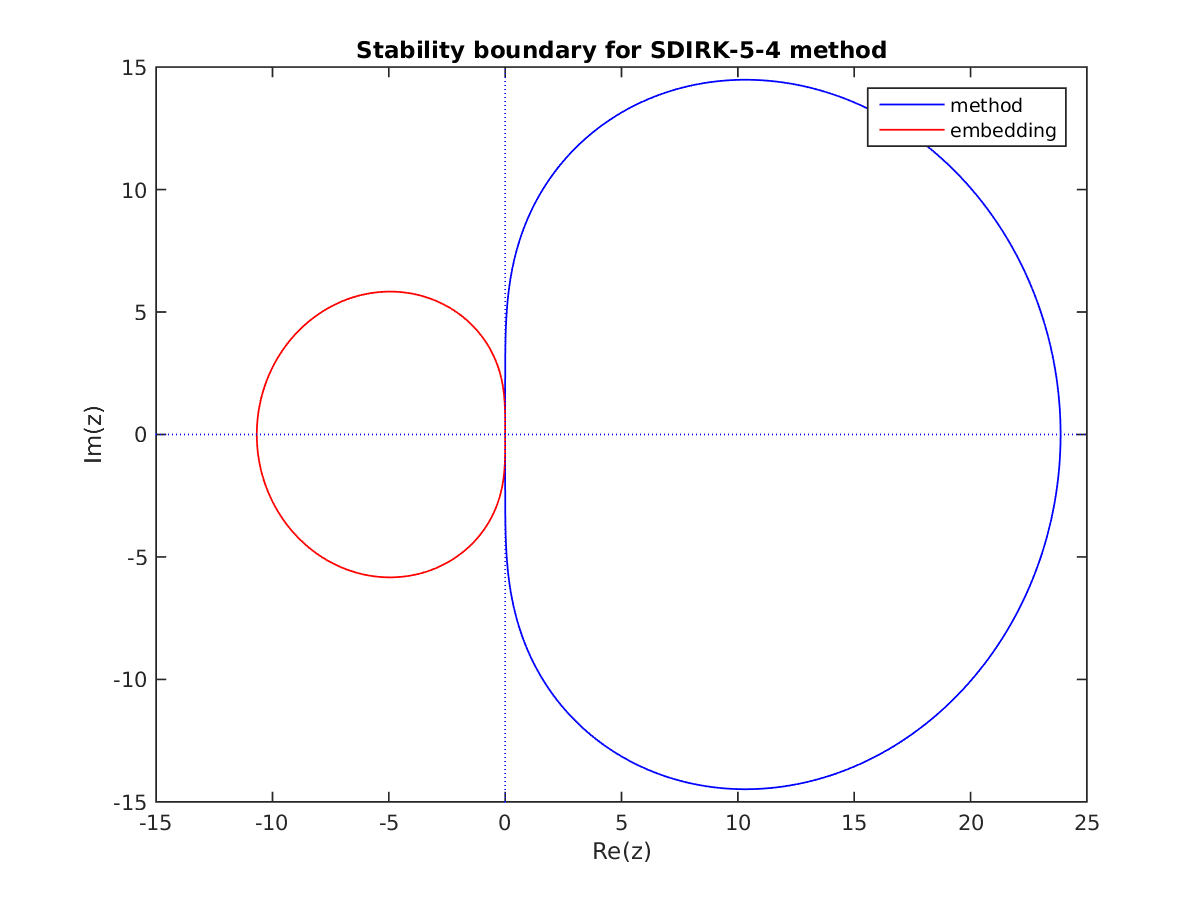
\includegraphics{stab_region_18.png}}
\caption{Linear stability region for the SDIRK-5-3-4 method.  The method's
region is outlined in blue; the embedding's region is in red.}\end{figure}


\subsection{Kvaerno-5-3-4}
\label{Butcher:kvaerno-5-3-4}\label{Butcher:butcher-kvaerno-5-3-4}
\index{Kvaerno-5-3-4 ESDIRK method}
Accessible via the constant \code{KVAERNO\_5\_3\_4} to
{\hyperref[ARKStep_c_interface/User_callable:c.ARKStepSetTableNum]{\emph{\code{ARKStepSetTableNum()}}}} or
{\hyperref[ARKodeButcherTable:c.ARKodeButcherTable_LoadDIRK]{\emph{\code{ARKodeButcherTable\_LoadDIRK()}}}}.  Both the method and embedding are
A-stable (from \phantomsection\label{Butcher:id22}{\hyperref[References:k2004]{\emph{{[}K2004{]}}}}).
\begin{gather}
\begin{split}\renewcommand{\arraystretch}{1.5}
\begin{array}{r|ccccc}
  0 & 0 & 0 & 0 & 0 & 0 \\
  0.871733043 & 0.4358665215  & 0.4358665215  & 0 & 0 & 0 \\
  0.468238744853136 & 0.140737774731968 & -0.108365551378832 & 0.4358665215 & 0 & 0 \\
  1 & 0.102399400616089 & -0.376878452267324 & 0.838612530151233 & 0.4358665215 & 0 \\
  1 & 0.157024897860995 & 0.117330441357768 & 0.61667803039168 & -0.326899891110444 & 0.4358665215 \\
  \hline
  4 & 0.157024897860995 & 0.117330441357768 & 0.61667803039168 & -0.326899891110444 & 0.4358665215 \\
  3 & 0.102399400616089 & -0.376878452267324 & 0.838612530151233 & 0.4358665215 & 0
\end{array}\end{split}\notag
\end{gather}\begin{figure}[htbp]
\centering
\capstart

\scalebox{0.500000}{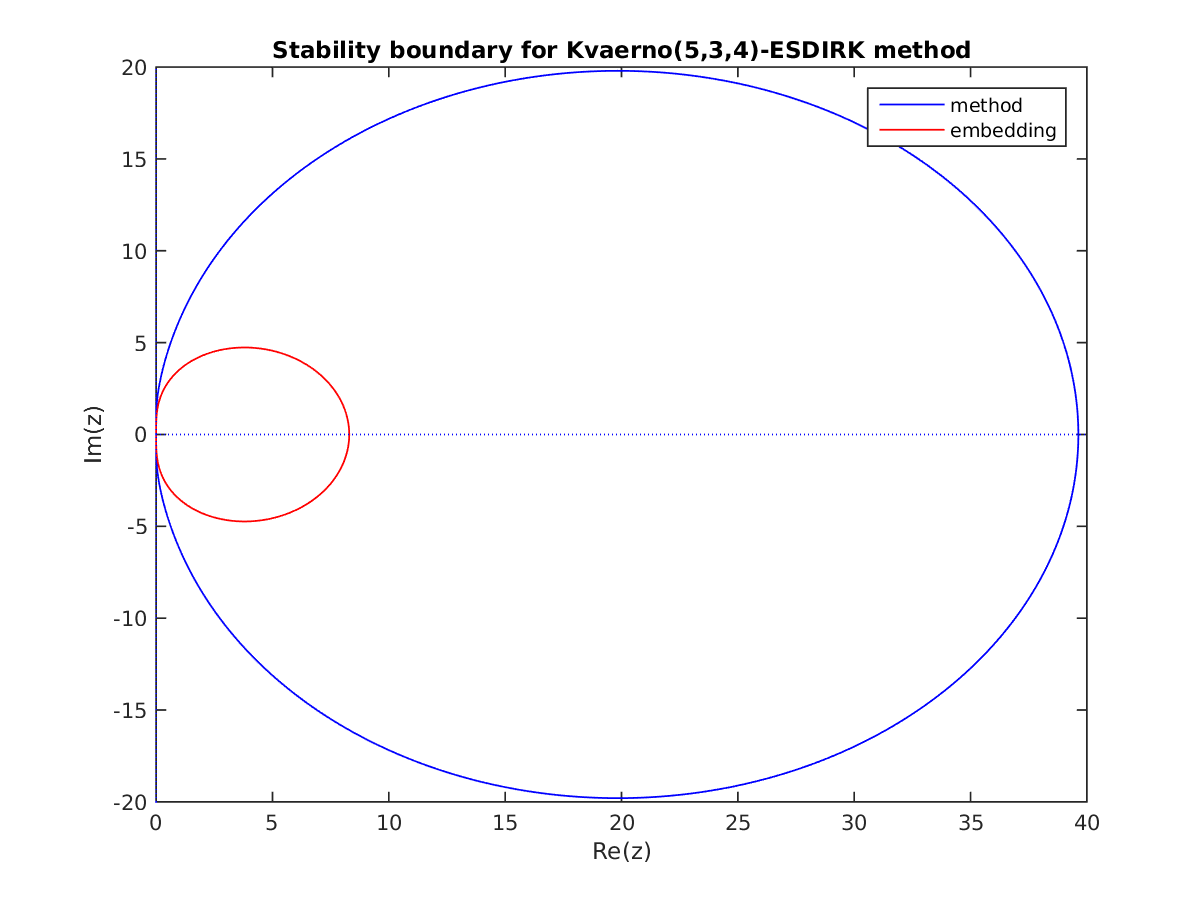
\includegraphics{stab_region_19.png}}
\caption{Linear stability region for the Kvaerno-5-3-4 method.  The method's
region is outlined in blue; the embedding's region is in red.}\end{figure}


\subsection{ARK-6-3-4 (implicit)}
\label{Butcher:ark-6-3-4-implicit}\label{Butcher:butcher-ark-6-3-4-i}
\index{ARK-6-3-4 ESDIRK method}
Accessible via the constant \code{ARK436L2SA\_DIRK\_6\_3\_4} to
{\hyperref[ARKStep_c_interface/User_callable:c.ARKStepSetTableNum]{\emph{\code{ARKStepSetTableNum()}}}} or
{\hyperref[ARKodeButcherTable:c.ARKodeButcherTable_LoadDIRK]{\emph{\code{ARKodeButcherTable\_LoadDIRK()}}}}.  This is the implicit portion
of the default 4th order additive method. Both the method and
embedding are A-stable; additionally the method is L-stable (from \phantomsection\label{Butcher:id23}{\hyperref[References:kc2003]{\emph{{[}KC2003{]}}}}).
\begin{gather}
\begin{split}\renewcommand{\arraystretch}{1.5}
\begin{array}{r|cccccc}
  0 & 0 & 0 & 0 & 0 & 0 & 0 \\
  \frac{1}{2} & \frac{1}{4} & \frac{1}{4} & 0 & 0 & 0 & 0 \\
  \frac{83}{250} & \frac{8611}{62500} & -\frac{1743}{31250} & \frac{1}{4} & 0 & 0 & 0 \\
  \frac{31}{50} & \frac{5012029}{34652500} & -\frac{654441}{2922500} & \frac{174375}{388108} & \frac{1}{4} & 0 & 0 \\
  \frac{17}{20} & \frac{15267082809}{155376265600} & -\frac{71443401}{120774400} & \frac{730878875}{902184768} & \frac{2285395}{8070912} & \frac{1}{4} & 0 \\
  1 & \frac{82889}{524892} & 0 & \frac{15625}{83664} & \frac{69875}{102672} & -\frac{2260}{8211} & \frac{1}{4} \\
  \hline
  4 & \frac{82889}{524892} & 0 & \frac{15625}{83664} & \frac{69875}{102672} & -\frac{2260}{8211} & \frac{1}{4} \\
  3 & \frac{4586570599}{29645900160} & 0 & \frac{178811875}{945068544} & \frac{814220225}{1159782912} & -\frac{3700637}{11593932} & \frac{61727}{225920}
\end{array}\end{split}\notag
\end{gather}\begin{figure}[htbp]
\centering
\capstart

\scalebox{0.500000}{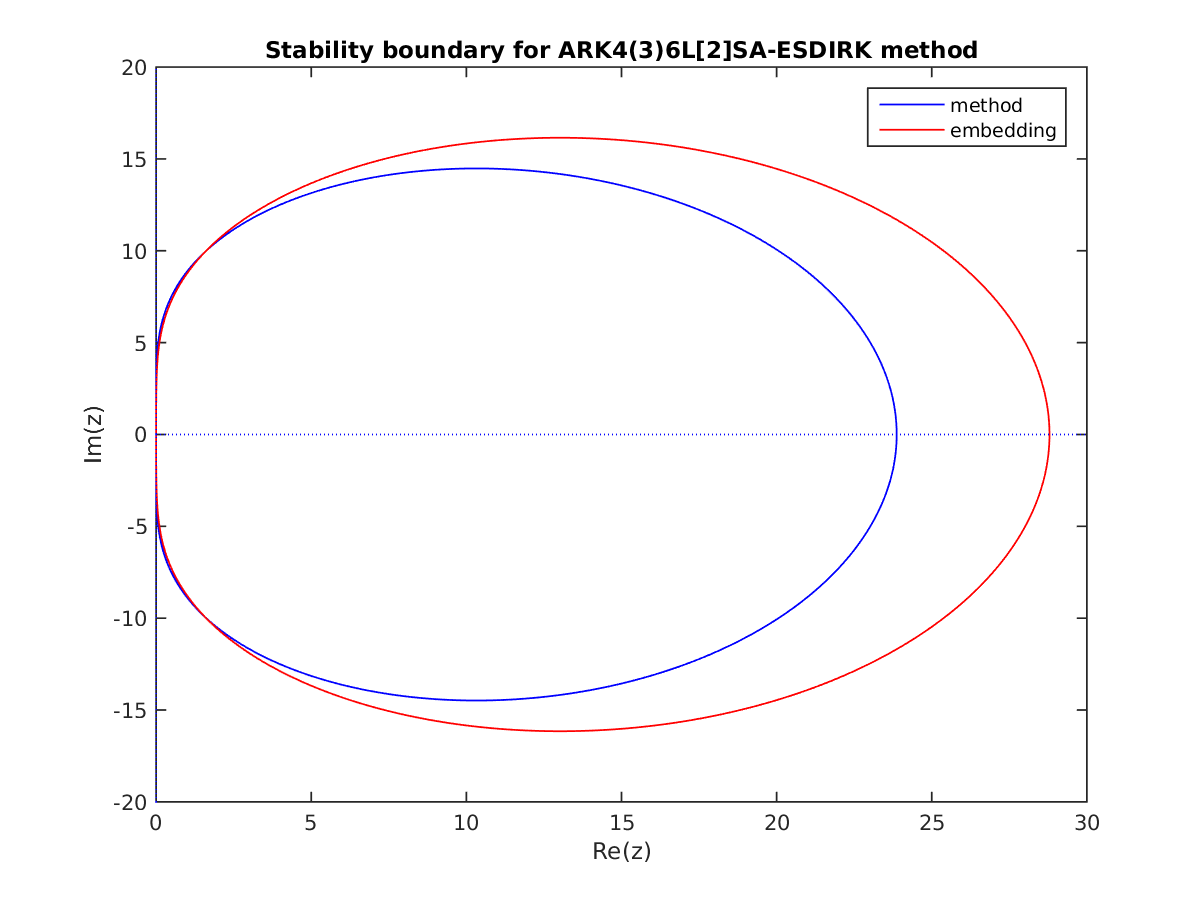
\includegraphics{stab_region_20.png}}
\caption{Linear stability region for the implicit ARK-6-3-4 method.  The method's
region is outlined in blue; the embedding's region is in red.}\end{figure}


\subsection{ARK-7-3-4 (implicit)}
\label{Butcher:butcher-ark-7-3-4-i}\label{Butcher:ark-7-3-4-implicit}
\index{ARK-7-3-4 ESDIRK method}
Accessible via the constant \code{ARK437L2SA\_DIRK\_7\_3\_4} to
{\hyperref[ARKStep_c_interface/User_callable:c.ARKStepSetTableNum]{\emph{\code{ARKStepSetTableNum()}}}} or
{\hyperref[ARKodeButcherTable:c.ARKodeButcherTable_LoadDIRK]{\emph{\code{ARKodeButcherTable\_LoadDIRK()}}}}.  This is the implicit portion
of the 4th order additive method from \phantomsection\label{Butcher:id24}{\hyperref[References:kc2019]{\emph{{[}KC2019{]}}}}.
\begin{gather}
\begin{split}\renewcommand{\arraystretch}{1.5}
\begin{array}{r|ccccccc}
  0 & 0 & 0 & 0 & 0 & 0 & 0 & 0 \\
  \frac{247}{1000} & \frac{1235}{10000} & \frac{1235}{10000} & 0 & 0 & 0 & 0 & 0 \\
  \frac{4276536705230}{10142255878289} & \frac{624185399699}{4186980696204} & \frac{624185399699}{4186980696204} & \frac{1235}{10000} & 0 & 0 & 0 & 0 \\
  \frac{67}{200} & \frac{1258591069120}{10082082980243} & \frac{1258591069120}{10082082980243} & -\frac{322722984531}{8455138723562} & \frac{1235}{10000} & 0 & 0 & 0 \\
  \frac{3}{40} & -\frac{436103496990}{5971407786587} & -\frac{436103496990}{5971407786587} & -\frac{2689175662187}{11046760208243} & \frac{4431412449334}{12995360898505} & \frac{1235}{10000} & 0 & 0 \\
  \frac{7}{10} & -\frac{2207373168298}{14430576638973} & -\frac{2207373168298}{14430576638973} & \frac{242511121179}{3358618340039} & \frac{3145666661981}{7780404714551} & \frac{5882073923981}{14490790706663} & \frac{1235}{10000} & 0 \\
  1 & 0 & 0 & \frac{9164257142617}{17756377923965} & -\frac{10812980402763}{74029279521829} & \frac{1335994250573}{5691609445217} & \frac{2273837961795}{8368240463276} & \frac{1235}{10000} \\
  \hline
  4 & 0 & 0 & \frac{9164257142617}{17756377923965} & -\frac{10812980402763}{74029279521829} & \frac{1335994250573}{5691609445217} & \frac{2273837961795}{8368240463276} & \frac{1235}{10000} \\
  3 & 0 & 0 & \frac{4469248916618}{8635866897933} & -\frac{621260224600}{4094290005349} & \frac{696572312987}{2942599194819} & \frac{1532940081127}{5565293938103} & \frac{2441}{20000}
\end{array}\end{split}\notag
\end{gather}

\subsection{Kvaerno-7-4-5}
\label{Butcher:kvaerno-7-4-5}\label{Butcher:butcher-kvaerno-7-4-5}
\index{Kvaerno-7-4-5 ESDIRK method}
Accessible via the constant \code{KVAERNO\_7\_4\_5} to
{\hyperref[ARKStep_c_interface/User_callable:c.ARKStepSetTableNum]{\emph{\code{ARKStepSetTableNum()}}}} or
{\hyperref[ARKodeButcherTable:c.ARKodeButcherTable_LoadDIRK]{\emph{\code{ARKodeButcherTable\_LoadDIRK()}}}}.  Both the method and embedding are
A-stable; additionally the method is L-stable (from \phantomsection\label{Butcher:id25}{\hyperref[References:k2004]{\emph{{[}K2004{]}}}}).
\begin{gather}
\begin{split}\renewcommand{\arraystretch}{1.5}
\begin{array}{r|ccccccc}
  0 & 0 & 0 & 0 & 0 & 0 & 0 & 0 \\
  0.52 & 0.26 & 0.26 & 0 & 0 & 0 & 0 & 0 \\
  1.230333209967908 & 0.13 & 0.84033320996790809 & 0.26 & 0 & 0 & 0 & 0 \\
  0.895765984350076 & 0.22371961478320505 & 0.47675532319799699 & -0.06470895363112615 & 0.26 & 0 & 0 & 0 \\
  0.436393609858648 & 0.16648564323248321 & 0.10450018841591720 & 0.03631482272098715 & -0.13090704451073998 & 0.26 & 0 & 0 \\
  1 & 0.13855640231268224 & 0 & -0.04245337201752043 & 0.02446657898003141 & 0.61943039072480676 & 0.26 & 0 \\
  1 & 0.13659751177640291 & 0 & -0.05496908796538376 & -0.04118626728321046 & 0.62993304899016403 & 0.06962479448202728 & 0.26 \\
  \hline
  5 & 0.13659751177640291 & 0 & -0.05496908796538376 & -0.04118626728321046 & 0.62993304899016403 & 0.06962479448202728 & 0.26 \\
  4 & 0.13855640231268224 & 0 & -0.04245337201752043 & 0.02446657898003141 & 0.61943039072480676 & 0.26 & 0
\end{array}\end{split}\notag
\end{gather}\begin{figure}[htbp]
\centering
\capstart

\scalebox{0.500000}{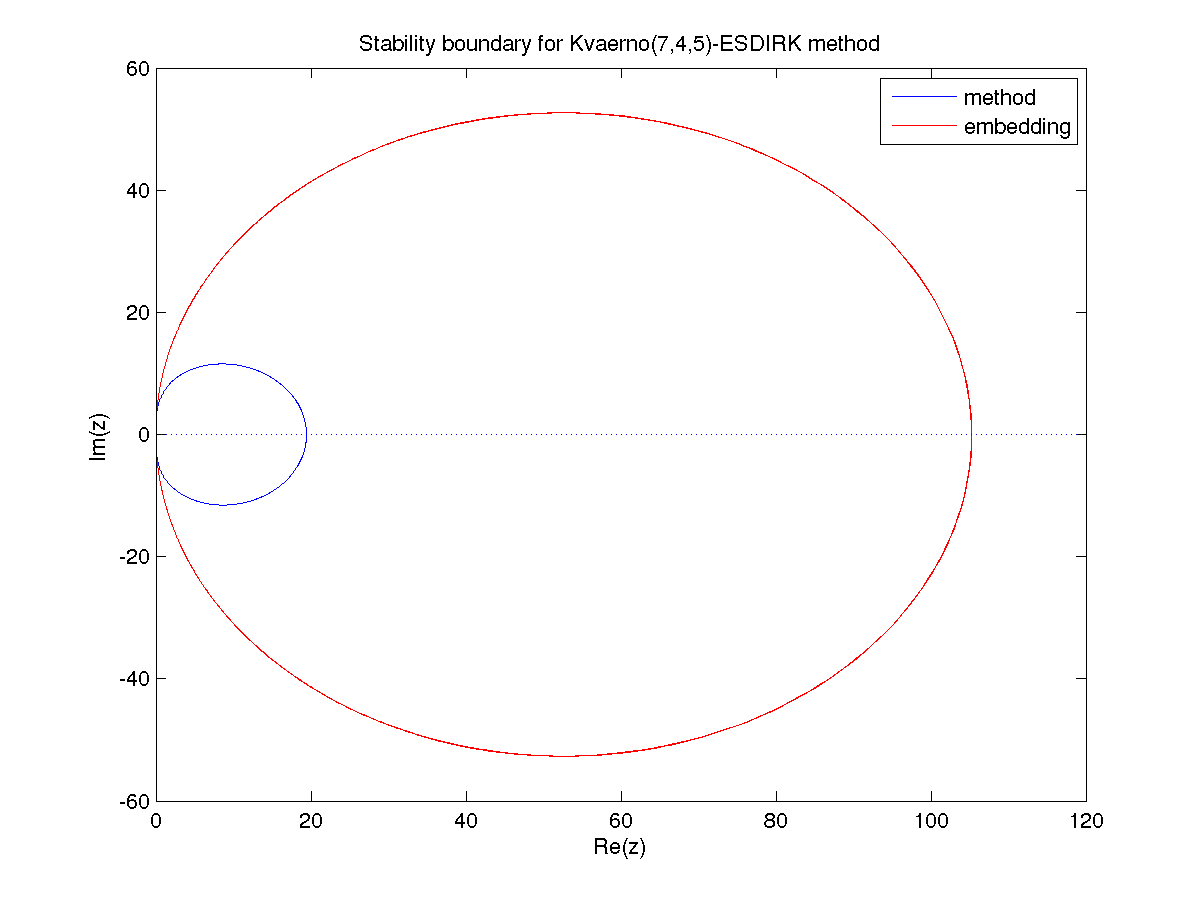
\includegraphics{stab_region_21.png}}
\caption{Linear stability region for the Kvaerno-7-4-5 method.  The method's
region is outlined in blue; the embedding's region is in red.}\end{figure}


\subsection{ARK-8-4-5 (implicit)}
\label{Butcher:ark-8-4-5-implicit}\label{Butcher:butcher-ark-8-4-5-i}
\index{ARK-8-4-5 ESDIRK method}
Accessible via the constant \code{ARK548L2SA\_DIRK\_8\_4\_5} for
{\hyperref[ARKStep_c_interface/User_callable:c.ARKStepSetTableNum]{\emph{\code{ARKStepSetTableNum()}}}} or
{\hyperref[ARKodeButcherTable:c.ARKodeButcherTable_LoadDIRK]{\emph{\code{ARKodeButcherTable\_LoadDIRK()}}}}.  This is the default 5th order
implicit method, and the implicit portion of the default 5th order
additive method.  Both the method and embedding are A-stable;
additionally the method is L-stable (from \phantomsection\label{Butcher:id26}{\hyperref[References:kc2003]{\emph{{[}KC2003{]}}}}).
\begin{gather}
\begin{split}\renewcommand{\arraystretch}{1.5}
\begin{array}{r|cccccccc}
  0 & 0 & 0 & 0 & 0 & 0 & 0 & 0 & 0 \\
  \frac{41}{100} & \frac{41}{200} & \frac{41}{200} & 0 & 0 & 0 & 0 & 0 & 0 \\
  \frac{2935347310677}{11292855782101} & \frac{41}{400} & -\frac{567603406766}{11931857230679} & \frac{41}{200} & 0 & 0 & 0 & 0 & 0 \\
  \frac{1426016391358}{7196633302097} & \frac{683785636431}{9252920307686} & 0 & -\frac{110385047103}{1367015193373} & \frac{41}{200} & 0 & 0 & 0 & 0 \\
  \frac{92}{100} & \frac{3016520224154}{10081342136671} & 0 & \frac{30586259806659}{12414158314087} & -\frac{22760509404356}{11113319521817} & \frac{41}{200} & 0 & 0 & 0 \\
  \frac{24}{100} & \frac{218866479029}{1489978393911} & 0 & \frac{638256894668}{5436446318841} & -\frac{1179710474555}{5321154724896} & -\frac{60928119172}{8023461067671} & \frac{41}{200} & 0 & 0 \\
  \frac{3}{5} & \frac{1020004230633}{5715676835656} & 0 & \frac{25762820946817}{25263940353407} & -\frac{2161375909145}{9755907335909} & -\frac{211217309593}{5846859502534} & -\frac{4269925059573}{7827059040749} & \frac{41}{200} & 0 \\
  1 & -\frac{872700587467}{9133579230613} & 0 & 0 & \frac{22348218063261}{9555858737531} & -\frac{1143369518992}{8141816002931} & -\frac{39379526789629}{19018526304540} & \frac{32727382324388}{42900044865799} & \frac{41}{200} \\
  \hline
  5 & -\frac{872700587467}{9133579230613} & 0 & 0 & \frac{22348218063261}{9555858737531} & -\frac{1143369518992}{8141816002931} & -\frac{39379526789629}{19018526304540} & \frac{32727382324388}{42900044865799} & \frac{41}{200} \\
  4 & -\frac{975461918565}{9796059967033} & 0 & 0 & \frac{78070527104295}{32432590147079} & -\frac{548382580838}{3424219808633} & -\frac{33438840321285}{15594753105479} & \frac{3629800801594}{4656183773603} & \frac{4035322873751}{18575991585200}
\end{array}\end{split}\notag
\end{gather}\begin{figure}[htbp]
\centering
\capstart

\scalebox{0.500000}{\includegraphics{stab_region_22.png}}
\caption{Linear stability region for the implicit ARK-8-4-5 method.  The method's
region is outlined in blue; the embedding's region is in red.}\end{figure}


\subsection{ARK-8-4-5b (implicit)}
\label{Butcher:butcher-ark-8-4-5b-i}\label{Butcher:ark-8-4-5b-implicit}
\index{ARK-8-4-5b ESDIRK method}
Accessible via the constant \code{ARK548L2SAb\_DIRK\_8\_4\_5} for
{\hyperref[ARKStep_c_interface/User_callable:c.ARKStepSetTableNum]{\emph{\code{ARKStepSetTableNum()}}}} or
{\hyperref[ARKodeButcherTable:c.ARKodeButcherTable_LoadDIRK]{\emph{\code{ARKodeButcherTable\_LoadDIRK()}}}}.  This is the 5th order
implicit method from \phantomsection\label{Butcher:id27}{\hyperref[References:kc2019]{\emph{{[}KC2019{]}}}}.
\begin{gather}
\begin{split}\renewcommand{\arraystretch}{1.5}
\begin{array}{r|cccccccc}
  0 & 0 & 0 & 0 & 0 & 0 & 0 & 0 & 0 \\
  \frac{4}{9} & \frac{2}{9} & \frac{2}{9} & 0 & 0 & 0 & 0 & 0 & 0 \\
  \frac{6456083330201}{8509243623797} & \frac{2366667076620}{8822750406821} & \frac{2366667076620}{8822750406821} & \frac{2}{9} & 0 & 0 & 0 & 0 & 0 \\
  \frac{1632083962415}{14158861528103} & -\frac{257962897183}{4451812247028} & -\frac{257962897183}{4451812247028} & \frac{128530224461}{14379561246022} & \frac{2}{9} & 0 & 0 & 0 & 0 \\
  \frac{6365430648612}{17842476412687} & -\frac{486229321650}{11227943450093} & -\frac{486229321650}{11227943450093} & -\frac{225633144460}{6633558740617} & \frac{1741320951451}{6824444397158} & \frac{2}{9} & 0 & 0 & 0 \\
  \frac{18}{25} & \frac{621307788657}{4714163060173} & \frac{621307788657}{4714163060173} & -\frac{125196015625}{3866852212004} & \frac{940440206406}{7593089888465} & \frac{961109811699}{6734810228204} & \frac{2}{9} & 0 & 0 \\
  \frac{191}{200} & \frac{2036305566805}{6583108094622} & \frac{2036305566805}{6583108094622} & -\frac{3039402635899}{4450598839912} & -\frac{1829510709469}{31102090912115} & -\frac{286320471013}{6931253422520} & \frac{8651533662697}{9642993110008} & \frac{2}{9} & 0 \\
  1 & 0 & 0 & \frac{3517720773327}{20256071687669} & \frac{4569610470461}{17934693873752} & \frac{2819471173109}{11655438449929} & \frac{3296210113763}{10722700128969} & -\frac{1142099968913}{5710983926999} & \frac{2}{9} \\
  \hline
  5 & 0 & 0 & \frac{3517720773327}{20256071687669} & \frac{4569610470461}{17934693873752} & \frac{2819471173109}{11655438449929} & \frac{3296210113763}{10722700128969} & -\frac{1142099968913}{5710983926999} & \frac{2}{9} \\
  4 & 0 & 0 & \frac{520639020421}{8300446712847} & \frac{4550235134915}{17827758688493} & \frac{1482366381361}{6201654941325} & \frac{5551607622171}{13911031047899} & -\frac{5266607656330}{36788968843917} & \frac{1074053359553}{5740751784926}
\end{array}\end{split}\notag
\end{gather}

\section{Additive Butcher tables}
\label{Butcher:additive-butcher-tables}\label{Butcher:butcher-additive}
In the category of additive Runge-Kutta methods for split implicit and
explicit calculations, ARKode includes methods that have orders 3
through 5, with embeddings that are of orders 2 through 4.  These
Butcher table pairs are as follows:
\begin{itemize}
\item {} 
\index{ARK-4-2-3 ARK method}3rd-order pair:
{\hyperref[Butcher:butcher-ark-4-2-3-e]{\emph{\DUspan{}{ARK-4-2-3 (explicit)}}}} with {\hyperref[Butcher:butcher-ark-4-2-3-i]{\emph{\DUspan{}{ARK-4-2-3 (implicit)}}}},
corresponding to Butcher tables \code{ARK324L2SA\_ERK\_4\_2\_3} and
\code{ARK324L2SA\_DIRK\_4\_2\_3} for {\hyperref[ARKStep_c_interface/User_callable:c.ARKStepSetTableNum]{\emph{\code{ARKStepSetTableNum()}}}}.

\item {} 
\index{ARK-6-3-4 ARK method}4th-order pair:
{\hyperref[Butcher:butcher-ark-6-3-4-e]{\emph{\DUspan{}{ARK-6-3-4 (explicit)}}}} with {\hyperref[Butcher:butcher-ark-6-3-4-i]{\emph{\DUspan{}{ARK-6-3-4 (implicit)}}}},
corresponding to Butcher tables \code{ARK436L2SA\_ERK\_6\_3\_4} and
\code{ARK436L2SA\_DIRK\_6\_3\_4} for {\hyperref[ARKStep_c_interface/User_callable:c.ARKStepSetTableNum]{\emph{\code{ARKStepSetTableNum()}}}}.

\item {} 
\index{ARK-7-3-4 ARK method}4th-order pair:
{\hyperref[Butcher:butcher-ark-7-3-4-e]{\emph{\DUspan{}{ARK-7-3-4 (explicit)}}}} with {\hyperref[Butcher:butcher-ark-7-3-4-i]{\emph{\DUspan{}{ARK-7-3-4 (implicit)}}}},
corresponding to Butcher tables \code{ARK437L2SA\_ERK\_7\_3\_4} and
\code{ARK437L2SA\_DIRK\_7\_3\_4} for {\hyperref[ARKStep_c_interface/User_callable:c.ARKStepSetTableNum]{\emph{\code{ARKStepSetTableNum()}}}}.

\item {} 
\index{ARK-8-4-5 ARK method}5th-order pair:
{\hyperref[Butcher:butcher-ark-8-4-5-e]{\emph{\DUspan{}{ARK-8-4-5 (explicit)}}}} with {\hyperref[Butcher:butcher-ark-8-4-5-i]{\emph{\DUspan{}{ARK-8-4-5 (implicit)}}}},
corresponding to Butcher tables \code{ARK548L2SA\_ERK\_8\_4\_5} and
\code{ARK548L2SA\_ERK\_8\_4\_5} for {\hyperref[ARKStep_c_interface/User_callable:c.ARKStepSetTableNum]{\emph{\code{ARKStepSetTableNum()}}}}.

\item {} 
\index{ARK-8-4-5b ARK method}5th-order pair:
{\hyperref[Butcher:butcher-ark-8-4-5b-e]{\emph{\DUspan{}{ARK-8-4-5b (explicit)}}}} with {\hyperref[Butcher:butcher-ark-8-4-5b-i]{\emph{\DUspan{}{ARK-8-4-5b (implicit)}}}},
corresponding to Butcher tables \code{ARK548L2SAb\_ERK\_8\_4\_5} and
\code{ARK548L2SAb\_ERK\_8\_4\_5} for {\hyperref[ARKStep_c_interface/User_callable:c.ARKStepSetTableNum]{\emph{\code{ARKStepSetTableNum()}}}}.

\end{itemize}


\chapter{Appendix: SUNDIALS Release History}
\label{History:appendix-sundials-release-history}\label{History::doc}\label{History:history}
\begin{longtable}{|l|l|l|l|l|l|l|l|}
\hline
\textsf{\relax 
Date
} & \textsf{\relax 
SUNDIALS
} & \textsf{\relax 
ARKode
} & \textsf{\relax 
CVODE
} & \textsf{\relax 
CVODES
} & \textsf{\relax 
IDA
} & \textsf{\relax 
IDAS
} & \textsf{\relax 
KINSOL
}\\
\hline\endfirsthead

\multicolumn{8}{c}%
{{\textsf{\tablename\ \thetable{} -- continued from previous page}}} \\
\hline
\textsf{\relax 
Date
} & \textsf{\relax 
SUNDIALS
} & \textsf{\relax 
ARKode
} & \textsf{\relax 
CVODE
} & \textsf{\relax 
CVODES
} & \textsf{\relax 
IDA
} & \textsf{\relax 
IDAS
} & \textsf{\relax 
KINSOL
}\\
\hline\endhead

\hline \multicolumn{8}{|r|}{{\textsf{Continued on next page}}} \\ \hline
\endfoot

\endlastfoot


Oct 2019
 & 
5.0.0
 & 
4.0.0
 & 
5.0.0
 & 
5.0.0
 & 
5.0.0
 & 
4.0.0
 & 
5.0.0
\\
\hline
Feb 2019
 & 
4.1.0
 & 
3.1.0
 & 
4.1.0
 & 
4.1.0
 & 
4.1.0
 & 
3.1.0
 & 
4.1.0
\\
\hline
Jan 2019
 & 
4.0.2
 & 
3.0.2
 & 
4.0.2
 & 
4.0.2
 & 
4.0.2
 & 
3.0.2
 & 
4.0.2
\\
\hline
Dec 2018
 & 
4.0.1
 & 
3.0.1
 & 
4.0.1
 & 
4.0.1
 & 
4.0.1
 & 
3.0.1
 & 
4.0.1
\\
\hline
Dec 2018
 & 
4.0.0
 & 
3.0.0
 & 
4.0.0
 & 
4.0.0
 & 
4.0.0
 & 
3.0.0
 & 
4.0.0
\\
\hline
Oct 2018
 & 
3.2.1
 & 
2.2.1
 & 
3.2.1
 & 
3.2.1
 & 
3.2.1
 & 
2.2.1
 & 
3.2.1
\\
\hline
Sep 2018
 & 
3.2.0
 & 
2.2.0
 & 
3.2.0
 & 
3.2.0
 & 
3.2.0
 & 
2.2.0
 & 
3.2.0
\\
\hline
Jul 2018
 & 
3.1.2
 & 
2.1.2
 & 
3.1.2
 & 
3.1.2
 & 
3.1.2
 & 
2.1.2
 & 
3.1.2
\\
\hline
May 2018
 & 
3.1.1
 & 
2.1.1
 & 
3.1.1
 & 
3.1.1
 & 
3.1.1
 & 
2.1.1
 & 
3.1.1
\\
\hline
Nov 2017
 & 
3.1.0
 & 
2.1.0
 & 
3.1.0
 & 
3.1.0
 & 
3.1.0
 & 
2.1.0
 & 
3.1.0
\\
\hline
Sep 2017
 & 
3.0.0
 & 
2.0.0
 & 
3.0.0
 & 
3.0.0
 & 
3.0.0
 & 
2.0.0
 & 
3.0.0
\\
\hline
Sep 2016
 & 
2.7.0
 & 
1.1.0
 & 
2.9.0
 & 
2.9.0
 & 
2.9.0
 & 
1.3.0
 & 
2.9.0
\\
\hline
Aug 2015
 & 
2.6.2
 & 
1.0.2
 & 
2.8.2
 & 
2.8.2
 & 
2.8.2
 & 
1.2.2
 & 
2.8.2
\\
\hline
Mar 2015
 & 
2.6.1
 & 
1.0.1
 & 
2.8.1
 & 
2.8.1
 & 
2.8.1
 & 
1.2.1
 & 
2.8.1
\\
\hline
Mar 2015
 & 
2.6.0
 & 
1.0.0
 & 
2.8.0
 & 
2.8.0
 & 
2.8.0
 & 
1.2.0
 & 
2.8.0
\\
\hline
Mar 2012
 & 
2.5.0
 & 
--
 & 
2.7.0
 & 
2.7.0
 & 
2.7.0
 & 
1.1.0
 & 
2.7.0
\\
\hline
May 2009
 & 
2.4.0
 & 
--
 & 
2.6.0
 & 
2.6.0
 & 
2.6.0
 & 
1.0.0
 & 
2.6.0
\\
\hline
Nov 2006
 & 
2.3.0
 & 
--
 & 
2.5.0
 & 
2.5.0
 & 
2.5.0
 & 
--
 & 
2.5.0
\\
\hline
Mar 2006
 & 
2.2.0
 & 
--
 & 
2.4.0
 & 
2.4.0
 & 
2.4.0
 & 
--
 & 
2.4.0
\\
\hline
May 2005
 & 
2.1.1
 & 
--
 & 
2.3.0
 & 
2.3.0
 & 
2.3.0
 & 
--
 & 
2.3.0
\\
\hline
Apr 2005
 & 
2.1.0
 & 
--
 & 
2.3.0
 & 
2.2.0
 & 
2.3.0
 & 
--
 & 
2.3.0
\\
\hline
Mar 2005
 & 
2.0.2
 & 
--
 & 
2.2.2
 & 
2.1.2
 & 
2.2.2
 & 
--
 & 
2.2.2
\\
\hline
Jan 2005
 & 
2.0.1
 & 
--
 & 
2.2.1
 & 
2.1.1
 & 
2.2.1
 & 
--
 & 
2.2.1
\\
\hline
Dec 2004
 & 
2.0.0
 & 
--
 & 
2.2.0
 & 
2.1.0
 & 
2.2.0
 & 
--
 & 
2.2.0
\\
\hline
Jul 2002
 & 
1.0.0
 & 
--
 & 
2.0.0
 & 
1.0.0
 & 
2.0.0
 & 
--
 & 
2.0.0
\\
\hline
Mar 2002
 & 
--
 & 
--
 & 
1.0.0 \footnote{
CVODE and PVODE combined
}
 & 
--
 & 
--
 & 
--
 & 
--
\\
\hline
Feb 1999
 & 
--
 & 
--
 & 
--
 & 
--
 & 
1.0.0 \footnote{
IDA written
}
 & 
--
 & 
--
\\
\hline
Aug 1998
 & 
--
 & 
--
 & 
--
 & 
--
 & 
--
 & 
--
 & 
1.0.0 \footnote{
KINSOL written
}
\\
\hline
Jul 1997
 & 
--
 & 
--
 & 
1.0.0 \footnote{
PVODE written
}
 & 
--
 & 
--
 & 
--
 & 
--
\\
\hline
Sep 1994
 & 
--
 & 
--
 & 
1.0.0 \footnote{
CVODE written
}
 & 
--
 & 
--
 & 
--
 & 
--
\\
\hline\end{longtable}

\phantomsection\label{References:references}
\begin{thebibliography}{SuperLUDIST}
\bibitem[A1965]{A1965}{\phantomsection\label{References:a1965} 
D.G. Anderson, Iterative Procedures for Nonlinear Integral
Equations, \emph{J. Assoc. Comput. Machinery},
12:547-560, 1965.
}
\bibitem[B1985]{B1985}{\phantomsection\label{References:b1985} 
Bank et al., Transient Simulation of Silicon Devices and
Circuits, \emph{IEEE Trans. CAD}, 4:436-451, 1985.
}
\bibitem[B1983]{B1983}{\phantomsection\label{References:b1983} 
S.R. Billington, Type-Insensitive Codes for the Solution of
Stiff and Nonstiff Systems of Ordinary Differential
Equations, \emph{in: Master Thesis, University of Manchester,
United Kingdom}, 1983.
}
\bibitem[BS1989]{BS1989}{\phantomsection\label{References:bs1989} 
P. Bogacki and L.F. Shampine. A 3(2) pair of Runge–Kutta
formulas, \emph{Appl. Math. Lett.}, 2:321–325, 1989.
}
\bibitem[B1987]{B1987}{\phantomsection\label{References:b1987} 
P.N. Brown. A local convergence theory for combined
inexact-Newton/finite difference projection
methods. \emph{SIAM J. Numer. Anal.}, 24:407-434, 1987.
}
\bibitem[BBH1989]{BBH1989}{\phantomsection\label{References:bbh1989} 
P.N. Brown, G.D. Byrne and A.C. Hindmarsh.  VODE, a
Variable-Coefficient ODE
Solver. \emph{SIAM J. Sci. Stat. Comput.}, 10:1038-1051, 1989.
}
\bibitem[BH1989]{BH1989}{\phantomsection\label{References:bh1989} 
P.N. Brown and A.C. Hindmarsh. Reduced Storage
Matrix Methods in Stiff ODE Systems. \emph{J. Appl. Math. \&
Comp.}, 31:49-91, 1989.
}
\bibitem[BS1990]{BS1990}{\phantomsection\label{References:bs1990} 
P.N. Brown and Y. Saad. Hybrid Krylov Methods for
Nonlinear Systems of Equations. \emph{SIAM J. Sci. Stat. Comput.}, 11:450-481, 1990.
}
\bibitem[B2008]{B2008}{\phantomsection\label{References:b2008} 
J.C. Butcher, Numerical Methods for Ordinary Differential
Equations. Wiley, 2nd edition, Chicester, England, 2008.
}
\bibitem[B1992]{B1992}{\phantomsection\label{References:b1992} 
G.D. Byrne. Pragmatic Experiments with Krylov Methods
in the Stiff ODE Setting.  In J.R. Cash and I. Gladwell,
editors, \emph{Computational Ordinary Differential Equations},
pp. 323-356, Oxford University Press, 1992.
}
\bibitem[C1979]{C1979}{\phantomsection\label{References:c1979} 
J.R. Cash. Diagonally Implicit Runge-Kutta Formulae with
Error Estimates. \emph{IMA J Appl Math}, 24:293-301, 1979.
}
\bibitem[CK1990]{CK1990}{\phantomsection\label{References:ck1990} 
J.R. Cash and A.H. Karp. A variable order Runge-Kutta
method for initial value problems with rapidly varying
right-hand sides, \emph{ACM Trans. Math. Soft.},
16:201-222, 1990.
}
\bibitem[CGM2014]{CGM2014}{\phantomsection\label{References:cgm2014} 
J. Cheng, M. Grossman and T. McKercher. Professional Cuda
C Programming.  John Wiley \& Sons, 2014.
}
\bibitem[cuSOLVER]{cuSOLVER}{\phantomsection\label{References:cusolver} 
\href{https://docs.nvidia.com/cuda/cusolver/index.html}{NVIDIA cuSOLVER Documentation}.
}
\bibitem[DP1980]{DP1980}{\phantomsection\label{References:dp1980} 
J.R. Dormand and P.J. Prince. A family of embedded
Runge-Kutta formulae, \emph{J. Comput. Appl. Math.} 6:19–26, 1980.
}
\bibitem[DP2010]{DP2010}{\phantomsection\label{References:dp2010} 
T. Davis and E. Palamadai Natarajan.  Algortithm 907: KLU,
a direct sparse solver for circuit simulation
problems. \emph{ACM Trans. Math. Soft.}, 37, 2010.
}
\bibitem[DES1982]{DES1982}{\phantomsection\label{References:des1982} 
R.S. Dembo, S.C. Eisenstat and T. Steihaug.  Inexact
Newton Methods. \emph{SIAM J. Numer. Anal.}, 19:400-408, 1982.
}
\bibitem[DGL1999]{DGL1999}{\phantomsection\label{References:dgl1999} 
J.W. Demmel, J.R. Gilbert and X.S. Li. An Asynchronous
Parallel Supernodal Algorithm for Sparse Gaussian
Elimination. \emph{SIAM J. Matrix Analysis and Applications},
20:915-952, 1999.
}
\bibitem[DS1996]{DS1996}{\phantomsection\label{References:ds1996} 
J.E. Dennis and R.B. Schnabel.  Numerical Methods for
Unconstrained Optimization and Nonlinear Equations. SIAM,
Philadelphia, 1996.
}
\bibitem[F2015]{F2015}{\phantomsection\label{References:f2015} 
R. Falgout and U.M. Yang. Hypre user's manual. \emph{LLNL
Technical Report}, 2015.
}
\bibitem[FS2009]{FS2009}{\phantomsection\label{References:fs2009} 
H. Fang and Y. Saad. Two classes of secant methods for
nonlinear acceleration. \emph{Numer. Linear Algebra Appl.},
16:197-21, 2009.
}
\bibitem[F1969]{F1969}{\phantomsection\label{References:f1969} 
E. Fehlberg. Low-order classical Runge-Kutta formulas with
step size control and their application to some heat
transfer problems. \emph{NASA Technical Report 315}, 1969.
}
\bibitem[F1993]{F1993}{\phantomsection\label{References:f1993} 
R.W. Freund. A Transpose-Free Quasi-Minimal Residual Algorithm
for Non-Hermitian Linear Systems. \emph{SIAM J. Sci. Comp.},
14:470-482, 1993.
}
\bibitem[G1991]{G1991}{\phantomsection\label{References:g1991} 
K. Gustafsson.  Control theoretic techniques for stepsize
selection in explicit Runge-Kutta methods. \emph{ACM
Trans. Math. Soft.}, 17:533-554, 1991.
}
\bibitem[G1994]{G1994}{\phantomsection\label{References:g1994} 
K. Gustafsson.  Control-theoretic techniques for stepsize
selection in implicit Runge-Kutta methods. \emph{ACM
Trans. Math. Soft.} 20:496-512, 1994.
}
\bibitem[GDL2007]{GDL2007}{\phantomsection\label{References:gdl2007} 
L. Grigori, J.W. Demmel, and X.S. Li. Parallel Symbolic
Factorization for Sparse LU with Static Pivoting. \emph{SIAM J.
Scientific Comptuing}, 29:1289-1314, 2007.
}
\bibitem[HW1993]{HW1993}{\phantomsection\label{References:hw1993} 
E. Hairer, S. Norsett and G. Wanner.  Solving Ordinary
Differential Equations I. \emph{Springer Series in
Computational Mathematics}, vol. 8, 1993.
}
\bibitem[HW1996]{HW1996}{\phantomsection\label{References:hw1996} 
E. Hairer and G. Wanner. Solving Ordinary Differential
Equations II. \emph{Springer Series in Computational
Mathematics}, vol. 14, 1996.
}
\bibitem[HS1952]{HS1952}{\phantomsection\label{References:hs1952} 
M.R. Hestenes and E. Stiefel. Methods of Conjugate
Gradients for Solving Linear Systems. \emph{J. Research of the
National Bureau of Standards}, 49:409-436, 1952.
}
\bibitem[HS1980]{HS1980}{\phantomsection\label{References:hs1980} 
K.L. Hiebert and L.F. Shampine.  Implicitly Defined Output
Points for Solutions of ODEs.  Technical Report
SAND80-0180, Sandia National Laboratories, February 1980.
}
\bibitem[H2000]{H2000}{\phantomsection\label{References:h2000} 
A.C. Hindmarsh. The PVODE and IDA Algorithms. Technical
Report UCRL-ID-141558, LLNL, 2000.
}
\bibitem[HS2017]{HS2017}{\phantomsection\label{References:hs2017} 
A.C. Hindmarsh and R. Serban. User Documentation for CVODE
v5.0.0. Technical Report UCRL-SM-208108, LLNL, 2019.
}
\bibitem[HSR2017]{HSR2017}{\phantomsection\label{References:hsr2017} 
A.C. Hindmarsh, R. Serban and D.R. Reynolds. Example
Programs for CVODE v5.0.0. Technical Report
UCRL-SM-208110, LLNL, 2019.
}
\bibitem[HT1998]{HT1998}{\phantomsection\label{References:ht1998} 
A.C. Hindmarsh and A.G. Taylor.  PVODE and KINSOL:
Parallel Software for Differential and Nonlinear
Systems. Technical Report UCRL-IL-129739, LLNL,
February 1998.
}
\bibitem[HK2014]{HK2014}{\phantomsection\label{References:hk2014} 
R.D. Hornung and J.A. Keasler.  The RAJA Portability
Layer: Overview and Status. Technical Report
LLNL-TR-661403, LLNL, September 2014.
}
\bibitem[JPE2019]{JPE2019}{\phantomsection\label{References:jpe2019} 
S.R. Johnson, A. Prokopenko, and K. J. Evans. Automated
Fortran-C++ bindings for Large-Scale Scientific Applications.
arXiv:1904.02546 {[}cs{]}, Apr. 2019.
}
\bibitem[K1995]{K1995}{\phantomsection\label{References:k1995} 
C.T. Kelley.  Iterative Methods for Solving Linear and
Nonlinear Equations. SIAM, Philadelphia, 1995.
}
\bibitem[KC2003]{KC2003}{\phantomsection\label{References:kc2003} 
C.A. Kennedy and M.H. Carpenter. Additive Runge-Kutta
schemes for convection-diffusion-reaction
equations. \emph{Appl. Numer. Math.}, 44:139-181, 2003.
}
\bibitem[KC2019]{KC2019}{\phantomsection\label{References:kc2019} 
C.A. Kennedy and M.H. Carpenter. Higher-order additive
Runge–Kutta schemes for ordinary differential
equations. \emph{Appl. Numer. Math.}, 136:183-205, 2019.
}
\bibitem[K2004]{K2004}{\phantomsection\label{References:k2004} 
A. Kv\{ae\}rno. Singly Diagonally Implicit Runge-Kutta
Methods with an Explicit First Stage. \emph{BIT Numer. Math.},
44:489-502, 2004.
}
\bibitem[KLU]{KLU}{\phantomsection\label{References:klu} 
\href{http://faculty.cse.tamu.edu/davis/suitesparse.html}{KLU Sparse Matrix Factorization Library}.
}
\bibitem[L2005]{L2005}{\phantomsection\label{References:l2005} 
X.S. Li. An Overview of SuperLU: Algorithms,
Implementation, and User Interface.
\emph{ACM Trans. Math. Soft.}, 31:302-325, 2005.
}
\bibitem[LD2003]{LD2003}{\phantomsection\label{References:ld2003} 
X.S. Li. and J.W. Demmel. A Scalable Distributed-Memory Sparse
Direct Solver for Unsymmetric Linear Systems.
\emph{ACM Trans. Math. Soft.}, 29:110-140, 2003.
}
\bibitem[LWWY2012]{LWWY2012}{\phantomsection\label{References:lwwy2012} 
P.A. Lott, H.F. Walker, C.S. Woodward and U.M. Yang. An
Accelerated Picard Method for Nonlinear Systems Related to
Variably Saturated Flow, \emph{Adv. Wat. Resour.}, 38:92-101, 2012.
}
\bibitem[R2018]{R2018}{\phantomsection\label{References:r2018} 
D.R. Reynolds. ARKode Example Documentation. Technical
Report, Southern Methodist University Center for Scientific
Computation, 2019.
}
\bibitem[SS1986]{SS1986}{\phantomsection\label{References:ss1986} 
Y. Saad and M.H. Schultz. GMRES: A Generalized Minimal Residual
Algorithm for Solving Nonsymmetric Linear Systems.
\emph{SIAM J. Sci. Stat. Comp.}, 7:856-869, 1986.
}
\bibitem[S1993]{S1993}{\phantomsection\label{References:s1993} 
Y. Saad. A flexible inner-outer preconditioned GMRES
algorithm.  \emph{SIAM J. Sci. Comput.}, 14:461-469, 1993.
}
\bibitem[SA2002]{SA2002}{\phantomsection\label{References:sa2002} 
A. Sayfy and A. Aburub. Embedded Additive Runge-Kutta
Methods. \emph{Intern. J. Computer Math.}, 79:945-953, 2002.
}
\bibitem[SKAW2009]{SKAW2009}{\phantomsection\label{References:skaw2009} 
M. Schlegel, O. Knoth, M. Arnold, and R. Wolke. Multirate
Runge--Kutta schemes for advection
equations. \emph{J. Comput. Appl. Math.}, 226:345-357, 2009.
}
\bibitem[SKAW2012a]{SKAW2012a}{\phantomsection\label{References:skaw2012a} 
M. Schlegel, O. Knoth, M. Arnold, and R. Wolke. Implementation of
multirate time integration methods for air pollution modelling.
\emph{GMD}, 5:1395-1405, 2012.
}
\bibitem[SKAW2012b]{SKAW2012b}{\phantomsection\label{References:skaw2012b} 
M. Schlegel, O. Knoth, M. Arnold, and R. Wolke. Numerical
solution of multiscale problems in atmospheric modeling.
\emph{Appl. Numer. Math.}, 62:1531-1542, 2012.
}
\bibitem[S1998]{S1998}{\phantomsection\label{References:s1998} 
G. Soderlind. The automatic control of numerical
integration.  \emph{CWI Quarterly}, 11:55-74, 1998.
}
\bibitem[S2003]{S2003}{\phantomsection\label{References:s2003} 
G. Soderlind. Digital filters in adaptive time-stepping.
\emph{ACM Trans. Math. Soft.}, 29:1-26, 2003.
}
\bibitem[S2006]{S2006}{\phantomsection\label{References:s2006} 
G. Soderlind. Time-step selection algorithms: Adaptivity,
control and signal processing. \emph{Appl. Numer. Math.},
56:488-502, 2006.
}
\bibitem[SLUUG1999]{SLUUG1999}{\phantomsection\label{References:sluug1999} 
X.S. Li, J.W. Demmel, J.R. Gilbert, L. Grigori,  M. Shao and
I. Yamazaki. SuperLU Users' Guide. 1999.
}
\bibitem[SuperLUDIST]{SuperLUDIST}{\phantomsection\label{References:superludist} 
\href{http://crd-legacy.lbl.gov/~xiaoye/SuperLU/}{SuperLU\_DIST Parallel Sparse Matrix Factorization Library}.
}
\bibitem[SuperLUMT]{SuperLUMT}{\phantomsection\label{References:superlumt} 
\href{http://crd-legacy.lbl.gov/~xiaoye/SuperLU/}{SuperLU\_MT Threaded Sparse Matrix Factorization Library}.
}
\bibitem[V1992]{V1992}{\phantomsection\label{References:v1992} 
H.A. Van Der Vorst. Bi-CGSTAB: A Fast and Smoothly Converging Variant
of Bi-CG for the Solution of Nonsymmetric Linear Systems. \emph{SIAM J. Sci. Stat. Comp.},
13:631-644, 1992.
}
\bibitem[V1978]{V1978}{\phantomsection\label{References:v1978} 
J.H. Verner. Explicit Runge-Kutta methods with estimates of
the local truncation error. \emph{SIAM J. Numer. Anal.},
15:772-790, 1978.
}
\bibitem[WN2011]{WN2011}{\phantomsection\label{References:wn2011} 
H.F. Walker and P. Ni. Anderson acceleration for
fixed-point iterations. \emph{SIAM J. Numer. Anal.},
49:1715-1735, 2011.
}
\bibitem[KW1998]{KW1998}{\phantomsection\label{References:kw1998} 
O. Knoth and R. Wolke. Implicit-explicit Runge-Kutta methods for
computing atmospheric reactive flows. \emph{Appl. Numer. Math.},
28(2):327-341, 1998.
}
\bibitem[Z1963]{Z1963}{\phantomsection\label{References:z1963} 
J.A. Zonneveld. Automatic integration of ordinary
differential equations. \emph{Report R743, Mathematisch Centrum},
Postbus 4079, 1009AB Amsterdam, 1963.
}
\end{thebibliography}



\renewcommand{\indexname}{Index}
\printindex
\end{document}
